\documentclass[]{book}
\usepackage{lmodern}
\usepackage{amssymb,amsmath}
\usepackage{ifxetex,ifluatex}
\usepackage{fixltx2e} % provides \textsubscript
\ifnum 0\ifxetex 1\fi\ifluatex 1\fi=0 % if pdftex
  \usepackage[T1]{fontenc}
  \usepackage[utf8]{inputenc}
\else % if luatex or xelatex
  \ifxetex
    \usepackage{mathspec}
  \else
    \usepackage{fontspec}
  \fi
  \defaultfontfeatures{Ligatures=TeX,Scale=MatchLowercase}
\fi
% use upquote if available, for straight quotes in verbatim environments
\IfFileExists{upquote.sty}{\usepackage{upquote}}{}
% use microtype if available
\IfFileExists{microtype.sty}{%
\usepackage{microtype}
\UseMicrotypeSet[protrusion]{basicmath} % disable protrusion for tt fonts
}{}
\usepackage[margin=1in]{geometry}
\usepackage{hyperref}
\hypersetup{unicode=true,
            pdftitle={Data Science for Biological, Medical and Health Research: Notes for 432},
            pdfauthor={Thomas E. Love, Ph.D.},
            pdfborder={0 0 0},
            breaklinks=true}
\urlstyle{same}  % don't use monospace font for urls
\usepackage{natbib}
\bibliographystyle{apalike}
\usepackage{color}
\usepackage{fancyvrb}
\newcommand{\VerbBar}{|}
\newcommand{\VERB}{\Verb[commandchars=\\\{\}]}
\DefineVerbatimEnvironment{Highlighting}{Verbatim}{commandchars=\\\{\}}
% Add ',fontsize=\small' for more characters per line
\usepackage{framed}
\definecolor{shadecolor}{RGB}{248,248,248}
\newenvironment{Shaded}{\begin{snugshade}}{\end{snugshade}}
\newcommand{\KeywordTok}[1]{\textcolor[rgb]{0.13,0.29,0.53}{\textbf{#1}}}
\newcommand{\DataTypeTok}[1]{\textcolor[rgb]{0.13,0.29,0.53}{#1}}
\newcommand{\DecValTok}[1]{\textcolor[rgb]{0.00,0.00,0.81}{#1}}
\newcommand{\BaseNTok}[1]{\textcolor[rgb]{0.00,0.00,0.81}{#1}}
\newcommand{\FloatTok}[1]{\textcolor[rgb]{0.00,0.00,0.81}{#1}}
\newcommand{\ConstantTok}[1]{\textcolor[rgb]{0.00,0.00,0.00}{#1}}
\newcommand{\CharTok}[1]{\textcolor[rgb]{0.31,0.60,0.02}{#1}}
\newcommand{\SpecialCharTok}[1]{\textcolor[rgb]{0.00,0.00,0.00}{#1}}
\newcommand{\StringTok}[1]{\textcolor[rgb]{0.31,0.60,0.02}{#1}}
\newcommand{\VerbatimStringTok}[1]{\textcolor[rgb]{0.31,0.60,0.02}{#1}}
\newcommand{\SpecialStringTok}[1]{\textcolor[rgb]{0.31,0.60,0.02}{#1}}
\newcommand{\ImportTok}[1]{#1}
\newcommand{\CommentTok}[1]{\textcolor[rgb]{0.56,0.35,0.01}{\textit{#1}}}
\newcommand{\DocumentationTok}[1]{\textcolor[rgb]{0.56,0.35,0.01}{\textbf{\textit{#1}}}}
\newcommand{\AnnotationTok}[1]{\textcolor[rgb]{0.56,0.35,0.01}{\textbf{\textit{#1}}}}
\newcommand{\CommentVarTok}[1]{\textcolor[rgb]{0.56,0.35,0.01}{\textbf{\textit{#1}}}}
\newcommand{\OtherTok}[1]{\textcolor[rgb]{0.56,0.35,0.01}{#1}}
\newcommand{\FunctionTok}[1]{\textcolor[rgb]{0.00,0.00,0.00}{#1}}
\newcommand{\VariableTok}[1]{\textcolor[rgb]{0.00,0.00,0.00}{#1}}
\newcommand{\ControlFlowTok}[1]{\textcolor[rgb]{0.13,0.29,0.53}{\textbf{#1}}}
\newcommand{\OperatorTok}[1]{\textcolor[rgb]{0.81,0.36,0.00}{\textbf{#1}}}
\newcommand{\BuiltInTok}[1]{#1}
\newcommand{\ExtensionTok}[1]{#1}
\newcommand{\PreprocessorTok}[1]{\textcolor[rgb]{0.56,0.35,0.01}{\textit{#1}}}
\newcommand{\AttributeTok}[1]{\textcolor[rgb]{0.77,0.63,0.00}{#1}}
\newcommand{\RegionMarkerTok}[1]{#1}
\newcommand{\InformationTok}[1]{\textcolor[rgb]{0.56,0.35,0.01}{\textbf{\textit{#1}}}}
\newcommand{\WarningTok}[1]{\textcolor[rgb]{0.56,0.35,0.01}{\textbf{\textit{#1}}}}
\newcommand{\AlertTok}[1]{\textcolor[rgb]{0.94,0.16,0.16}{#1}}
\newcommand{\ErrorTok}[1]{\textcolor[rgb]{0.64,0.00,0.00}{\textbf{#1}}}
\newcommand{\NormalTok}[1]{#1}
\usepackage{longtable,booktabs}
\usepackage{graphicx,grffile}
\makeatletter
\def\maxwidth{\ifdim\Gin@nat@width>\linewidth\linewidth\else\Gin@nat@width\fi}
\def\maxheight{\ifdim\Gin@nat@height>\textheight\textheight\else\Gin@nat@height\fi}
\makeatother
% Scale images if necessary, so that they will not overflow the page
% margins by default, and it is still possible to overwrite the defaults
% using explicit options in \includegraphics[width, height, ...]{}
\setkeys{Gin}{width=\maxwidth,height=\maxheight,keepaspectratio}
\IfFileExists{parskip.sty}{%
\usepackage{parskip}
}{% else
\setlength{\parindent}{0pt}
\setlength{\parskip}{6pt plus 2pt minus 1pt}
}
\setlength{\emergencystretch}{3em}  % prevent overfull lines
\providecommand{\tightlist}{%
  \setlength{\itemsep}{0pt}\setlength{\parskip}{0pt}}
\setcounter{secnumdepth}{5}
% Redefines (sub)paragraphs to behave more like sections
\ifx\paragraph\undefined\else
\let\oldparagraph\paragraph
\renewcommand{\paragraph}[1]{\oldparagraph{#1}\mbox{}}
\fi
\ifx\subparagraph\undefined\else
\let\oldsubparagraph\subparagraph
\renewcommand{\subparagraph}[1]{\oldsubparagraph{#1}\mbox{}}
\fi

%%% Use protect on footnotes to avoid problems with footnotes in titles
\let\rmarkdownfootnote\footnote%
\def\footnote{\protect\rmarkdownfootnote}

%%% Change title format to be more compact
\usepackage{titling}

% Create subtitle command for use in maketitle
\newcommand{\subtitle}[1]{
  \posttitle{
    \begin{center}\large#1\end{center}
    }
}

\setlength{\droptitle}{-2em}
  \title{Data Science for Biological, Medical and Health Research: Notes for 432}
  \pretitle{\vspace{\droptitle}\centering\huge}
  \posttitle{\par}
  \author{Thomas E. Love, Ph.D.}
  \preauthor{\centering\large\emph}
  \postauthor{\par}
  \predate{\centering\large\emph}
  \postdate{\par}
  \date{Built 2018-05-01 10:10:30}

\usepackage{booktabs}
\usepackage{amsthm}
\makeatletter
\def\thm@space@setup{%
  \thm@preskip=8pt plus 2pt minus 4pt
  \thm@postskip=\thm@preskip
}
\makeatother

\usepackage{amsthm}
\newtheorem{theorem}{Theorem}[chapter]
\newtheorem{lemma}{Lemma}[chapter]
\theoremstyle{definition}
\newtheorem{definition}{Definition}[chapter]
\newtheorem{corollary}{Corollary}[chapter]
\newtheorem{proposition}{Proposition}[chapter]
\theoremstyle{definition}
\newtheorem{example}{Example}[chapter]
\theoremstyle{definition}
\newtheorem{exercise}{Exercise}[chapter]
\theoremstyle{remark}
\newtheorem*{remark}{Remark}
\newtheorem*{solution}{Solution}
\begin{document}
\maketitle

{
\setcounter{tocdepth}{1}
\tableofcontents
}
\chapter*{Introduction}\label{introduction}
\addcontentsline{toc}{chapter}{Introduction}

These Notes provide a series of examples using R to work through issues
that are likely to come up in PQHS/CRSP/MPHP 432.

While these Notes share some of the features of a textbook, they are
neither comprehensive nor completely original. The main purpose is to
give students in 432 a set of common materials on which to draw during
the course. In class, we will sometimes:

\begin{itemize}
\tightlist
\item
  reiterate points made in this document,
\item
  amplify what is here,
\item
  simplify the presentation of things done here,
\item
  use new examples to show some of the same techniques,
\item
  refer to issues not mentioned in this document,
\end{itemize}

but what we don't (always) do is follow these notes very precisely. We
assume instead that you will read the materials and try to learn from
them, just as you will attend classes and try to learn from them. We
welcome feedback of all kinds on this document or anything else. Just
email us at \texttt{431-help\ at\ case\ dot\ edu}, or submit a pull
request. Note that we still use \texttt{431-help} even though we're now
in 432.

What you will mostly find are brief explanations of a key idea or
summary, accompanied (most of the time) by R code and a demonstration of
the results of applying that code.

Everything you see here is available to you as HTML or PDF. You will
also have access to the R Markdown files, which contain the code which
generates everything in the document, including all of the R results. We
will demonstrate the use of R Markdown (this document is generated with
the additional help of an R package called bookdown) and R Studio (the
``program'' which we use to interface with the R language) in class.

To download the data and R code related to these notes, visit the Data
and Code section of \href{https://github.com/THOMASELOVE/432-2018}{the
432 course website}.

\chapter*{R Packages used in these
notes}\label{r-packages-used-in-these-notes}
\addcontentsline{toc}{chapter}{R Packages used in these notes}

Here, we'll load in the packages used in these notes.

\begin{Shaded}
\begin{Highlighting}[]
\KeywordTok{library}\NormalTok{(tableone)}
\KeywordTok{library}\NormalTok{(skimr)}
\KeywordTok{library}\NormalTok{(ggridges)}
\KeywordTok{library}\NormalTok{(magrittr)}
\KeywordTok{library}\NormalTok{(pander)}
\KeywordTok{library}\NormalTok{(arm)}
\KeywordTok{library}\NormalTok{(survival)}
\KeywordTok{library}\NormalTok{(OIsurv)}
\KeywordTok{library}\NormalTok{(survminer)}
\KeywordTok{library}\NormalTok{(rms)}
\KeywordTok{library}\NormalTok{(leaps)}
\KeywordTok{library}\NormalTok{(lars)}
\KeywordTok{library}\NormalTok{(Epi)}
\KeywordTok{library}\NormalTok{(pROC)}
\KeywordTok{library}\NormalTok{(ROCR)}
\KeywordTok{library}\NormalTok{(simputation)}
\KeywordTok{library}\NormalTok{(modelr)}
\KeywordTok{library}\NormalTok{(broom)}
\KeywordTok{library}\NormalTok{(tidyverse)}
\end{Highlighting}
\end{Shaded}

\chapter*{Data used in these notes}\label{data-used-in-these-notes}
\addcontentsline{toc}{chapter}{Data used in these notes}

Here, we'll load in the data sets used in these notes.

\begin{Shaded}
\begin{Highlighting}[]
\NormalTok{fakestroke <-}\StringTok{ }\KeywordTok{read.csv}\NormalTok{(}\StringTok{"data/fakestroke.csv"}\NormalTok{) }\OperatorTok\StringTok{ }\NormalTok{tbl_df}
\NormalTok{bloodbrain <-}\StringTok{ }\KeywordTok{read.csv}\NormalTok{(}\StringTok{"data/bloodbrain.csv"}\NormalTok{) }\OperatorTok\StringTok{ }\NormalTok{tbl_df}
\NormalTok{smartcle1 <-}\StringTok{ }\KeywordTok{read.csv}\NormalTok{(}\StringTok{"data/smartcle1.csv"}\NormalTok{) }\OperatorTok\StringTok{ }\NormalTok{tbl_df}
\NormalTok{bonding <-}\StringTok{ }\KeywordTok{read.csv}\NormalTok{(}\StringTok{"data/bonding.csv"}\NormalTok{) }\OperatorTok\StringTok{ }\NormalTok{tbl_df}
\NormalTok{cortisol <-}\StringTok{ }\KeywordTok{read.csv}\NormalTok{(}\StringTok{"data/cortisol.csv"}\NormalTok{) }\OperatorTok\StringTok{ }\NormalTok{tbl_df}
\NormalTok{emphysema <-}\StringTok{ }\KeywordTok{read.csv}\NormalTok{(}\StringTok{"data/emphysema.csv"}\NormalTok{) }\OperatorTok\StringTok{ }\NormalTok{tbl_df}
\NormalTok{prost <-}\StringTok{ }\KeywordTok{read.csv}\NormalTok{(}\StringTok{"data/prost.csv"}\NormalTok{) }\OperatorTok\StringTok{ }\NormalTok{tbl_df}
\NormalTok{pollution <-}\StringTok{ }\KeywordTok{read.csv}\NormalTok{(}\StringTok{"data/pollution.csv"}\NormalTok{) }\OperatorTok\StringTok{ }\NormalTok{tbl_df}
\NormalTok{resect <-}\StringTok{ }\KeywordTok{read.csv}\NormalTok{(}\StringTok{"data/resect.csv"}\NormalTok{) }\OperatorTok\StringTok{ }\NormalTok{tbl_df}
\NormalTok{colscr <-}\StringTok{ }\KeywordTok{read.csv}\NormalTok{(}\StringTok{"data/screening.csv"}\NormalTok{) }\OperatorTok\StringTok{ }\NormalTok{tbl_df}
\NormalTok{colscr2 <-}\StringTok{ }\KeywordTok{read.csv}\NormalTok{(}\StringTok{"data/screening2.csv"}\NormalTok{) }\OperatorTok\StringTok{ }\NormalTok{tbl_df}
\NormalTok{authorship <-}\StringTok{ }\KeywordTok{read_csv}\NormalTok{(}\StringTok{"data/authorship.csv"}\NormalTok{) }
\end{Highlighting}
\end{Shaded}

\begin{verbatim}
Parsed with column specification:
cols(
  .default = col_integer(),
  Author = col_character()
)
\end{verbatim}

\begin{verbatim}
See spec(...) for full column specifications.
\end{verbatim}

\begin{Shaded}
\begin{Highlighting}[]
\NormalTok{hem <-}\StringTok{ }\KeywordTok{read.csv}\NormalTok{(}\StringTok{"data/hem.csv"}\NormalTok{) }\OperatorTok\StringTok{ }\NormalTok{tbl_df}
\NormalTok{leukem <-}\StringTok{ }\KeywordTok{read.csv}\NormalTok{(}\StringTok{"data/leukem.csv"}\NormalTok{) }\OperatorTok\StringTok{ }\NormalTok{tbl_df}
\end{Highlighting}
\end{Shaded}

\chapter*{Special Functions used in these
notes}\label{special-functions-used-in-these-notes}
\addcontentsline{toc}{chapter}{Special Functions used in these notes}

\begin{Shaded}
\begin{Highlighting}[]
\NormalTok{specify_decimal <-}\StringTok{ }\ControlFlowTok{function}\NormalTok{(x, k) }\KeywordTok{format}\NormalTok{(}\KeywordTok{round}\NormalTok{(x, k), }\DataTypeTok{nsmall=}\NormalTok{k)}
\KeywordTok{skim_with}\NormalTok{(}\DataTypeTok{numeric =} \KeywordTok{list}\NormalTok{(}\DataTypeTok{hist =} \OtherTok{NULL}\NormalTok{), }
          \DataTypeTok{integer =} \KeywordTok{list}\NormalTok{(}\DataTypeTok{hist =} \OtherTok{NULL}\NormalTok{), }
          \DataTypeTok{ts =} \KeywordTok{list}\NormalTok{(}\DataTypeTok{line_graph =} \OtherTok{NULL}\NormalTok{))}
\end{Highlighting}
\end{Shaded}

\chapter{Building Table 1}\label{building-table-1}

Many scientific articles involve direct comparison of results from
various exposures, perhaps treatments. In 431, we studied numerous
methods, including various sorts of hypothesis tests, confidence
intervals, and descriptive summaries, which can help us to understand
and compare outcomes in such a setting. One common approach is to
present what's often called Table 1. Table 1 provides a summary of the
characteristics of a sample, or of groups of samples, which is most
commonly used to help understand the nature of the data being compared.

\section{\texorpdfstring{Two examples from the \emph{New England Journal
of
Medicine}}{Two examples from the New England Journal of Medicine}}\label{two-examples-from-the-new-england-journal-of-medicine}

\subsection{A simple Table 1}\label{a-simple-table-1}

Table 1 is especially common in the context of clinical research.
Consider the excerpt below, from a January 2015 article in the \emph{New
England Journal of Medicine} \citep{Tolaney2015}.

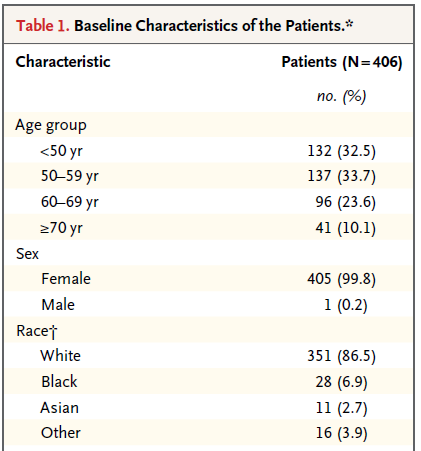
\includegraphics[width=0.5\linewidth]{images/Tolaney-snip1}

This (partial) table reports baseline characteristics on age group, sex
and race, describing 406 patients with HER2-positive\footnote{HER2 =
  human epidermal growth factor receptor type 2. Over-expression of this
  occurs in 15-20\% of invasive breast cancers, and has been associated
  with poor outcomes.} invasive breast cancer that began the protocol
therapy. Age, sex and race (along with severity of illness) are the most
commonly identified characteristics in a Table 1.

In addition to the measures shown in this excerpt, the full Table also
includes detailed information on the primary tumor for each patient,
including its size, nodal status and histologic grade. Footnotes tell us
that the percentages shown are subject to rounding, and may not total
100, and that the race information was self-reported.

\subsection{A group comparison}\label{a-group-comparison}

A more typical Table 1 involves a group comparison, for example in this
excerpt from \citet{Roy2008}. This Table 1 describes a multi-center
randomized clinical trial comparing two different approaches to caring
for patients with heart failure and atrial fibrillation\footnote{The
  complete Table 1 appears on pages 2668-2669 of \citet{Roy2008}, but I
  have only reproduced the first page and the footnote in this excerpt.}.

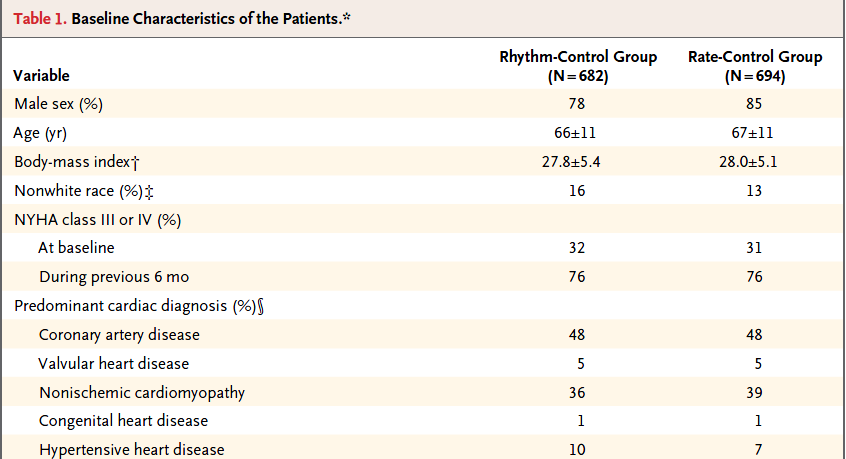
\includegraphics[width=0.9\linewidth]{images/Roy-snip1}

The article provides percentages, means and standard deviations across
groups, but note that it does not provide p values for the comparison of
baseline characteristics. This is a common feature of NEJM reports on
randomized clinical trials, where we anticipate that the two groups will
be well matched at baseline. Note that the patients in this study were
\emph{randomly} assigned to either the rhythm-control group or to the
rate-control group, using blocked randomizations stratified by study
center.

\section{The MR CLEAN trial}\label{the-mr-clean-trial}

\citet{Berkhemer2015} reported on the MR CLEAN trial, involving 500
patients with acute ischemic stroke caused by a proximal intracranial
arterial occlusion. The trial was conducted at 16 medical centers in the
Netherlands, where 233 were randomly assigned to the intervention
(intraarterial treatment plus usual care) and 267 to control (usual care
alone.) The primary outcome was the modified Rankin scale score at 90
days; this categorical scale measures functional outcome, with scores
ranging from 0 (no symptoms) to 6 (death). The fundamental conclusion of
\citet{Berkhemer2015} was that in patients with acute ischemic stroke
caused by a proximal intracranial occlusion of the anterior circulation,
intraarterial treatment administered within 6 hours after stroke onset
was effective and safe.

Here's the Table 1 from \citet{Berkhemer2015}.

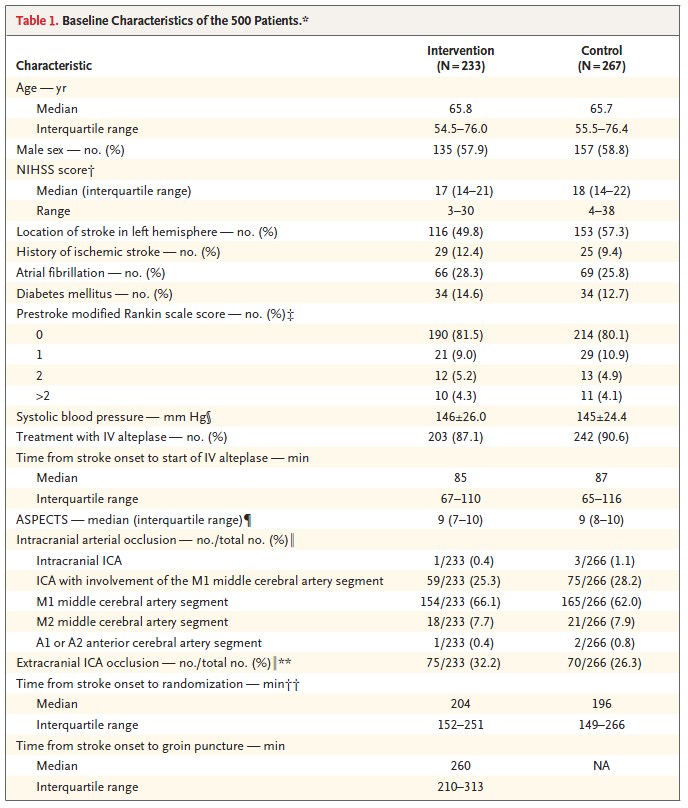
\includegraphics[width=0.9\linewidth]{images/Berkhemer-snip4complete}

The Table was accompanied by the following notes.

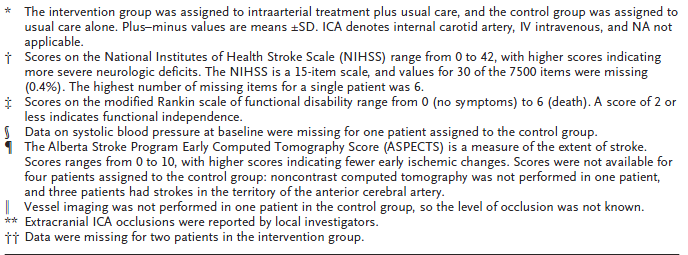
\includegraphics[width=0.9\linewidth]{images/Berkhemer-snip4notes}

\section{\texorpdfstring{Simulated \texttt{fakestroke}
data}{Simulated fakestroke data}}\label{simulated-fakestroke-data}

Consider the simulated data, available on the Data and Code page of
\href{https://github.com/THOMASELOVE/432-2018}{our course website} in
the \texttt{fakestroke.csv} file, which I built to let us mirror the
Table 1 for MR CLEAN \citep{Berkhemer2015}. The \texttt{fakestroke.csv}
file contains the following 18 variables for 500 patients.

\begin{longtable}[]{@{}rl@{}}
\toprule
\begin{minipage}[b]{0.16\columnwidth}\raggedleft\strut
Variable\strut
\end{minipage} & \begin{minipage}[b]{0.55\columnwidth}\raggedright\strut
Description\strut
\end{minipage}\tabularnewline
\midrule
\endhead
\begin{minipage}[t]{0.16\columnwidth}\raggedleft\strut
\texttt{studyid}\strut
\end{minipage} & \begin{minipage}[t]{0.55\columnwidth}\raggedright\strut
Study ID \# (z001 through z500)\strut
\end{minipage}\tabularnewline
\begin{minipage}[t]{0.16\columnwidth}\raggedleft\strut
\texttt{trt}\strut
\end{minipage} & \begin{minipage}[t]{0.55\columnwidth}\raggedright\strut
Treatment group (Intervention or Control)\strut
\end{minipage}\tabularnewline
\begin{minipage}[t]{0.16\columnwidth}\raggedleft\strut
\texttt{age}\strut
\end{minipage} & \begin{minipage}[t]{0.55\columnwidth}\raggedright\strut
Age in years\strut
\end{minipage}\tabularnewline
\begin{minipage}[t]{0.16\columnwidth}\raggedleft\strut
\texttt{sex}\strut
\end{minipage} & \begin{minipage}[t]{0.55\columnwidth}\raggedright\strut
Male or Female\strut
\end{minipage}\tabularnewline
\begin{minipage}[t]{0.16\columnwidth}\raggedleft\strut
\texttt{nihss}\strut
\end{minipage} & \begin{minipage}[t]{0.55\columnwidth}\raggedright\strut
NIH Stroke Scale Score (can range from 0-42; higher scores indicate more
severe neurological deficits)\strut
\end{minipage}\tabularnewline
\begin{minipage}[t]{0.16\columnwidth}\raggedleft\strut
\texttt{location}\strut
\end{minipage} & \begin{minipage}[t]{0.55\columnwidth}\raggedright\strut
Stroke Location - Left or Right Hemisphere\strut
\end{minipage}\tabularnewline
\begin{minipage}[t]{0.16\columnwidth}\raggedleft\strut
\texttt{hx.isch}\strut
\end{minipage} & \begin{minipage}[t]{0.55\columnwidth}\raggedright\strut
History of Ischemic Stroke (Yes/No)\strut
\end{minipage}\tabularnewline
\begin{minipage}[t]{0.16\columnwidth}\raggedleft\strut
\texttt{afib}\strut
\end{minipage} & \begin{minipage}[t]{0.55\columnwidth}\raggedright\strut
Atrial Fibrillation (1 = Yes, 0 = No)\strut
\end{minipage}\tabularnewline
\begin{minipage}[t]{0.16\columnwidth}\raggedleft\strut
\texttt{dm}\strut
\end{minipage} & \begin{minipage}[t]{0.55\columnwidth}\raggedright\strut
Diabetes Mellitus (1 = Yes, 0 = No)\strut
\end{minipage}\tabularnewline
\begin{minipage}[t]{0.16\columnwidth}\raggedleft\strut
\texttt{mrankin}\strut
\end{minipage} & \begin{minipage}[t]{0.55\columnwidth}\raggedright\strut
Pre-stroke modified Rankin scale score (0, 1, 2 or \textgreater{} 2)
indicating functional disability - complete range is 0 (no symptoms) to
6 (death)\strut
\end{minipage}\tabularnewline
\begin{minipage}[t]{0.16\columnwidth}\raggedleft\strut
\texttt{sbp}\strut
\end{minipage} & \begin{minipage}[t]{0.55\columnwidth}\raggedright\strut
Systolic blood pressure, in mm Hg\strut
\end{minipage}\tabularnewline
\begin{minipage}[t]{0.16\columnwidth}\raggedleft\strut
\texttt{iv.altep}\strut
\end{minipage} & \begin{minipage}[t]{0.55\columnwidth}\raggedright\strut
Treatment with IV alteplase (Yes/No)\strut
\end{minipage}\tabularnewline
\begin{minipage}[t]{0.16\columnwidth}\raggedleft\strut
\texttt{time.iv}\strut
\end{minipage} & \begin{minipage}[t]{0.55\columnwidth}\raggedright\strut
Time from stroke onset to start of IV alteplase (minutes) if
iv.altep=Yes\strut
\end{minipage}\tabularnewline
\begin{minipage}[t]{0.16\columnwidth}\raggedleft\strut
\texttt{aspects}\strut
\end{minipage} & \begin{minipage}[t]{0.55\columnwidth}\raggedright\strut
Alberta Stroke Program Early Computed Tomography score, which measures
extent of stroke from 0 - 10; higher scores indicate fewer early
ischemic changes\strut
\end{minipage}\tabularnewline
\begin{minipage}[t]{0.16\columnwidth}\raggedleft\strut
\texttt{ia.occlus}\strut
\end{minipage} & \begin{minipage}[t]{0.55\columnwidth}\raggedright\strut
Intracranial arterial occlusion, based on vessel imaging - five
categories\footnotemark{}\strut
\end{minipage}
\footnotetext{The five categories are Intracranial ICA, ICA with
  involvement of the M1 middle cerebral artery segment, M1 middle
  cerebral artery segment, M2 middle cerebral artery segment, A1 or A2
  anterior cerebral artery segment}\tabularnewline
\begin{minipage}[t]{0.16\columnwidth}\raggedleft\strut
\texttt{extra.ica}\strut
\end{minipage} & \begin{minipage}[t]{0.55\columnwidth}\raggedright\strut
Extracranial ICA occlusion (1 = Yes, 0 = No)\strut
\end{minipage}\tabularnewline
\begin{minipage}[t]{0.16\columnwidth}\raggedleft\strut
\texttt{time.rand}\strut
\end{minipage} & \begin{minipage}[t]{0.55\columnwidth}\raggedright\strut
Time from stroke onset to study randomization, in minutes\strut
\end{minipage}\tabularnewline
\begin{minipage}[t]{0.16\columnwidth}\raggedleft\strut
\texttt{time.punc}\strut
\end{minipage} & \begin{minipage}[t]{0.55\columnwidth}\raggedright\strut
Time from stroke onset to groin puncture, in minutes (only if
Intervention)\strut
\end{minipage}\tabularnewline
\bottomrule
\end{longtable}

Here's a quick look at the simulated data in \texttt{fakestroke}.

\begin{Shaded}
\begin{Highlighting}[]
\NormalTok{fakestroke}
\end{Highlighting}
\end{Shaded}

\begin{verbatim}
# A tibble: 500 x 18
   studyid trt        age sex   nihss location hx.isch  afib    dm mrankin
   <fct>   <fct>    <dbl> <fct> <int> <fct>    <fct>   <int> <int> <fct>  
 1 z001    Control    53. Male     21 Right    No          0     0 2      
 2 z002    Interve~   51. Male     23 Left     No          1     0 0      
 3 z003    Control    68. Fema~    11 Right    No          0     0 0      
 4 z004    Control    28. Male     22 Left     No          0     0 0      
 5 z005    Control    91. Male     24 Right    No          0     0 0      
 6 z006    Control    34. Fema~    18 Left     No          0     0 2      
 7 z007    Interve~   75. Male     25 Right    No          0     0 0      
 8 z008    Control    89. Fema~    18 Right    No          0     0 0      
 9 z009    Control    75. Male     25 Left     No          1     0 2      
10 z010    Interve~   26. Fema~    27 Right    No          0     0 0      
# ... with 490 more rows, and 8 more variables: sbp <int>, iv.altep <fct>,
#   time.iv <int>, aspects <int>, ia.occlus <fct>, extra.ica <int>,
#   time.rand <int>, time.punc <int>
\end{verbatim}

\section{\texorpdfstring{Building Table 1 for \texttt{fakestroke}:
Attempt
1}{Building Table 1 for fakestroke: Attempt 1}}\label{building-table-1-for-fakestroke-attempt-1}

Our goal, then, is to take the data in \texttt{fakestroke.csv} and use
it to generate a Table 1 for the study that compares the 233 patients in
the Intervention group to the 267 patients in the Control group, on all
of the other variables (except study ID \#) available. I'll use the
\texttt{tableone} package of functions available in R to help me
complete this task. We'll make a first attempt, using the
\texttt{CreateTableOne} function in the \texttt{tableone} package. To
use the function, we'll need to specify:

\begin{itemize}
\tightlist
\item
  the \texttt{vars} or variables we want to place in the rows of our
  Table 1 (which will include just about everything in the
  \texttt{fakestroke} data except the \texttt{studyid} code and the
  \texttt{trt} variable for which we have other plans, and the
  \texttt{time.punc} which applies only to subjects in the Intervention
  group.)

  \begin{itemize}
  \tightlist
  \item
    A useful trick here is to use the \texttt{dput} function,
    specifically something like \texttt{dput(names(fakestroke))} can be
    used to generate a list of all of the variables included in the
    \texttt{fakestroke} tibble, and then this can be copied and pasted
    into the \texttt{vars} specification, saving some typing.
  \end{itemize}
\item
  the \texttt{strata} which indicates the levels want to use in the
  columns of our Table 1 (for us, that's \texttt{trt})
\end{itemize}

\begin{Shaded}
\begin{Highlighting}[]
\NormalTok{fs.vars <-}\StringTok{ }\KeywordTok{c}\NormalTok{(}\StringTok{"age"}\NormalTok{, }\StringTok{"sex"}\NormalTok{, }\StringTok{"nihss"}\NormalTok{, }\StringTok{"location"}\NormalTok{, }
          \StringTok{"hx.isch"}\NormalTok{, }\StringTok{"afib"}\NormalTok{, }\StringTok{"dm"}\NormalTok{, }\StringTok{"mrankin"}\NormalTok{, }\StringTok{"sbp"}\NormalTok{,}
          \StringTok{"iv.altep"}\NormalTok{, }\StringTok{"time.iv"}\NormalTok{, }\StringTok{"aspects"}\NormalTok{, }
          \StringTok{"ia.occlus"}\NormalTok{, }\StringTok{"extra.ica"}\NormalTok{, }\StringTok{"time.rand"}\NormalTok{)}

\NormalTok{fs.trt <-}\StringTok{ }\KeywordTok{c}\NormalTok{(}\StringTok{"trt"}\NormalTok{)}

\NormalTok{att1 <-}\StringTok{ }\KeywordTok{CreateTableOne}\NormalTok{(}\DataTypeTok{data =}\NormalTok{ fakestroke, }
                       \DataTypeTok{vars =}\NormalTok{ fs.vars, }
                       \DataTypeTok{strata =}\NormalTok{ fs.trt)}
\KeywordTok{print}\NormalTok{(att1)}
\end{Highlighting}
\end{Shaded}

\begin{verbatim}
                       Stratified by trt
                        Control        Intervention   p      test
  n                        267            233                    
  age (mean (sd))        65.38 (16.10)  63.93 (18.09)  0.343     
  sex = Male (%)           157 (58.8)     135 (57.9)   0.917     
  nihss (mean (sd))      18.08 (4.32)   17.97 (5.04)   0.787     
  location = Right (%)     114 (42.7)     117 (50.2)   0.111     
  hx.isch = Yes (%)         25 ( 9.4)      29 (12.4)   0.335     
  afib (mean (sd))        0.26 (0.44)    0.28 (0.45)   0.534     
  dm (mean (sd))          0.13 (0.33)    0.12 (0.33)   0.923     
  mrankin (%)                                          0.922     
     > 2                    11 ( 4.1)      10 ( 4.3)             
     0                     214 (80.1)     190 (81.5)             
     1                      29 (10.9)      21 ( 9.0)             
     2                      13 ( 4.9)      12 ( 5.2)             
  sbp (mean (sd))       145.00 (24.40) 146.03 (26.00)  0.647     
  iv.altep = Yes (%)       242 (90.6)     203 (87.1)   0.267     
  time.iv (mean (sd))    87.96 (26.01)  98.22 (45.48)  0.003     
  aspects (mean (sd))     8.65 (1.47)    8.35 (1.64)   0.033     
  ia.occlus (%)                                        0.795     
     A1 or A2                2 ( 0.8)       1 ( 0.4)             
     ICA with M1            75 (28.2)      59 (25.3)             
     Intracranial ICA        3 ( 1.1)       1 ( 0.4)             
     M1                    165 (62.0)     154 (66.1)             
     M2                     21 ( 7.9)      18 ( 7.7)             
  extra.ica (mean (sd))   0.26 (0.44)    0.32 (0.47)   0.150     
  time.rand (mean (sd)) 213.88 (70.29) 202.51 (57.33)  0.051     
\end{verbatim}

\subsection{Some of this is very useful, and other parts need to be
fixed.}\label{some-of-this-is-very-useful-and-other-parts-need-to-be-fixed.}

\begin{enumerate}
\def\labelenumi{\arabic{enumi}.}
\tightlist
\item
  The 1/0 variables (\texttt{afib}, \texttt{dm}, \texttt{extra.ica})
  might be better if they were treated as the factors they are, and
  reported as the Yes/No variables are reported, with counts and
  percentages rather than with means and standard deviations.
\item
  In some cases, we may prefer to re-order the levels of the categorical
  (factor) variables, particularly the \texttt{mrankin} variable, but
  also the \texttt{ia.occlus} variable. It would also be more typical to
  put the Intervention group to the left and the Control group to the
  right, so we may need to adjust our \texttt{trt} variable's levels
  accordingly.
\item
  For each of the quantitative variables (\texttt{age}, \texttt{nihss},
  \texttt{sbp}, \texttt{time.iv}, \texttt{aspects}, \texttt{extra.ica},
  \texttt{time.rand} and \texttt{time.punc}) we should make a decision
  whether a summary with mean and standard deviation is appropriate, or
  whether we should instead summarize with, say, the median and
  quartiles. A mean and standard deviation really only yields an
  appropriate summary when the data are least approximately Normally
  distributed. This will make the \emph{p} values a bit more reasonable,
  too. The \texttt{test} column in the first attempt will soon have
  something useful to tell us.
\item
  If we'd left in the \texttt{time.punc} variable, we'd get some
  warnings, having to do with the fact that \texttt{time.punc} is only
  relevant to patients in the Intervention group.
\end{enumerate}

\subsection{\texorpdfstring{\texttt{fakestroke} Cleaning Up Categorical
Variables}{fakestroke Cleaning Up Categorical Variables}}\label{fakestroke-cleaning-up-categorical-variables}

Let's specify each of the categorical variables as categorical
explicitly. This helps the \texttt{CreateTableOne} function treat them
appropriately, and display them with counts and percentages. This
includes all of the 1/0, Yes/No and multi-categorical variables.

\begin{Shaded}
\begin{Highlighting}[]
\NormalTok{fs.factorvars <-}\StringTok{ }\KeywordTok{c}\NormalTok{(}\StringTok{"sex"}\NormalTok{, }\StringTok{"location"}\NormalTok{, }\StringTok{"hx.isch"}\NormalTok{, }\StringTok{"afib"}\NormalTok{, }\StringTok{"dm"}\NormalTok{, }
                   \StringTok{"mrankin"}\NormalTok{, }\StringTok{"iv.altep"}\NormalTok{, }\StringTok{"ia.occlus"}\NormalTok{, }\StringTok{"extra.ica"}\NormalTok{)}
\end{Highlighting}
\end{Shaded}

Then we simply add a \texttt{factorVars\ =\ fs.factorvars} call to the
\texttt{CreateTableOne} function.

We also want to re-order some of those categorical variables, so that
the levels are more useful to us. Specifically, we want to:

\begin{itemize}
\tightlist
\item
  place Intervention before Control in the \texttt{trt} variable,
\item
  reorder the \texttt{mrankin} scale as 0, 1, 2, \textgreater{} 2, and
\item
  rearrange the \texttt{ia.occlus} variable to the order\footnote{We
    might also have considered reordering the \texttt{ia.occlus} factor
    by its frequency, using the \texttt{fct\_infreq} function} presented
  in \citet{Berkhemer2015}.
\end{itemize}

To accomplish this, we'll use the \texttt{fct\_relevel} function from
the \texttt{forcats} package (loaded with the rest of the core
\texttt{tidyverse} packages) to reorder our levels manually.

\begin{Shaded}
\begin{Highlighting}[]
\NormalTok{fakestroke <-}\StringTok{ }\NormalTok{fakestroke }\OperatorTok
\StringTok{    }\KeywordTok{mutate}\NormalTok{(}\DataTypeTok{trt =} \KeywordTok{fct_relevel}\NormalTok{(trt, }\StringTok{"Intervention"}\NormalTok{, }\StringTok{"Control"}\NormalTok{),}
           \DataTypeTok{mrankin =} \KeywordTok{fct_relevel}\NormalTok{(mrankin, }\StringTok{"0"}\NormalTok{, }\StringTok{"1"}\NormalTok{, }\StringTok{"2"}\NormalTok{, }\StringTok{"> 2"}\NormalTok{),}
           \DataTypeTok{ia.occlus =} \KeywordTok{fct_relevel}\NormalTok{(ia.occlus, }\StringTok{"Intracranial ICA"}\NormalTok{, }
                                   \StringTok{"ICA with M1"}\NormalTok{, }\StringTok{"M1"}\NormalTok{, }\StringTok{"M2"}\NormalTok{, }
                                   \StringTok{"A1 or A2"}\NormalTok{)}
\NormalTok{           ) }
\end{Highlighting}
\end{Shaded}

\section{\texorpdfstring{\texttt{fakestroke} Table 1: Attempt
2}{fakestroke Table 1: Attempt 2}}\label{fakestroke-table-1-attempt-2}

\begin{Shaded}
\begin{Highlighting}[]
\NormalTok{att2 <-}\StringTok{ }\KeywordTok{CreateTableOne}\NormalTok{(}\DataTypeTok{data =}\NormalTok{ fakestroke, }
                       \DataTypeTok{vars =}\NormalTok{ fs.vars,}
                       \DataTypeTok{factorVars =}\NormalTok{ fs.factorvars,}
                       \DataTypeTok{strata =}\NormalTok{ fs.trt)}
\KeywordTok{print}\NormalTok{(att2)}
\end{Highlighting}
\end{Shaded}

\begin{verbatim}
                       Stratified by trt
                        Intervention   Control        p      test
  n                        233            267                    
  age (mean (sd))        63.93 (18.09)  65.38 (16.10)  0.343     
  sex = Male (%)           135 (57.9)     157 (58.8)   0.917     
  nihss (mean (sd))      17.97 (5.04)   18.08 (4.32)   0.787     
  location = Right (%)     117 (50.2)     114 (42.7)   0.111     
  hx.isch = Yes (%)         29 (12.4)      25 ( 9.4)   0.335     
  afib = 1 (%)              66 (28.3)      69 (25.8)   0.601     
  dm = 1 (%)                29 (12.4)      34 (12.7)   1.000     
  mrankin (%)                                          0.922     
     0                     190 (81.5)     214 (80.1)             
     1                      21 ( 9.0)      29 (10.9)             
     2                      12 ( 5.2)      13 ( 4.9)             
     > 2                    10 ( 4.3)      11 ( 4.1)             
  sbp (mean (sd))       146.03 (26.00) 145.00 (24.40)  0.647     
  iv.altep = Yes (%)       203 (87.1)     242 (90.6)   0.267     
  time.iv (mean (sd))    98.22 (45.48)  87.96 (26.01)  0.003     
  aspects (mean (sd))     8.35 (1.64)    8.65 (1.47)   0.033     
  ia.occlus (%)                                        0.795     
     Intracranial ICA        1 ( 0.4)       3 ( 1.1)             
     ICA with M1            59 (25.3)      75 (28.2)             
     M1                    154 (66.1)     165 (62.0)             
     M2                     18 ( 7.7)      21 ( 7.9)             
     A1 or A2                1 ( 0.4)       2 ( 0.8)             
  extra.ica = 1 (%)         75 (32.2)      70 (26.3)   0.179     
  time.rand (mean (sd)) 202.51 (57.33) 213.88 (70.29)  0.051     
\end{verbatim}

The categorical data presentation looks much improved.

\subsection{What summaries should we
show?}\label{what-summaries-should-we-show}

Now, we'll move on to the issue of making a decision about what type of
summary to show for the quantitative variables. Since the
\texttt{fakestroke} data are just simulated and only match the summary
statistics of the original results, not the details, we'll adopt the
decisions made by \citet{Berkhemer2015}, which were to use medians and
interquartile ranges to summarize the distributions of all of the
continuous variables \textbf{except} systolic blood pressure.

\begin{itemize}
\tightlist
\item
  Specifying certain quantitative variables as \emph{non-normal} causes
  R to show them with medians and the 25th and 75th percentiles, rather
  than means and standard deviations, and also causes those variables to
  be tested using non-parametric tests, like the Wilcoxon signed rank
  test, rather than the t test. The \texttt{test} column indicates this
  with the word \texttt{nonnorm}.

  \begin{itemize}
  \tightlist
  \item
    In real data situations, what should we do? The answer is to look at
    the data. I would not make the decision as to which approach to take
    without first plotting (perhaps in a histogram or a Normal Q-Q plot)
    the observed distributions in each of the two samples, so that I
    could make a sound decision about whether Normality was a reasonable
    assumption. If the means and medians are meaningfully different from
    each other, this is especially important.
  \item
    To be honest, though, if the variable in question is a relatively
    unimportant covariate and the \emph{p} values for the two approaches
    are nearly the same, I'd say that further investigation is rarely
    important,
  \end{itemize}
\item
  Specifying \emph{exact} tests for certain categorical variables (we'll
  try this for the \texttt{location} and \texttt{mrankin} variables) can
  be done, and these changes will be noted in the \texttt{test} column,
  as well.

  \begin{itemize}
  \tightlist
  \item
    In real data situations, I would rarely be concerned about this
    issue, and often choose Pearson (approximate) options across the
    board. This is reasonable so long as the number of subjects falling
    in each category is reasonably large, say above 10. If not, then an
    exact test may be a tiny improvement.
  \item
    Paraphrasing \citet{Rosenbaum2017}, having an exact rather than an
    approximate test result is about as valuable as having a nice crease
    in your trousers.
  \end{itemize}
\end{itemize}

To finish our Table 1, then, we need to specify which variables should
be treated as non-Normal in the \texttt{print} statement - notice that
we don't need to redo the \texttt{CreateTableOne} for this change.

\begin{Shaded}
\begin{Highlighting}[]
\KeywordTok{print}\NormalTok{(att2, }
      \DataTypeTok{nonnormal =} \KeywordTok{c}\NormalTok{(}\StringTok{"age"}\NormalTok{, }\StringTok{"nihss"}\NormalTok{, }\StringTok{"time.iv"}\NormalTok{, }\StringTok{"aspects"}\NormalTok{, }\StringTok{"time.rand"}\NormalTok{),}
      \DataTypeTok{exact =} \KeywordTok{c}\NormalTok{(}\StringTok{"location"}\NormalTok{, }\StringTok{"mrankin"}\NormalTok{))}
\end{Highlighting}
\end{Shaded}

\begin{verbatim}
                          Stratified by trt
                           Intervention            Control                
  n                           233                     267                 
  age (median [IQR])        65.80 [54.50, 76.00]    65.70 [55.75, 76.20]  
  sex = Male (%)              135 (57.9)              157 (58.8)          
  nihss (median [IQR])      17.00 [14.00, 21.00]    18.00 [14.00, 22.00]  
  location = Right (%)        117 (50.2)              114 (42.7)          
  hx.isch = Yes (%)            29 (12.4)               25 ( 9.4)          
  afib = 1 (%)                 66 (28.3)               69 (25.8)          
  dm = 1 (%)                   29 (12.4)               34 (12.7)          
  mrankin (%)                                                             
     0                        190 (81.5)              214 (80.1)          
     1                         21 ( 9.0)               29 (10.9)          
     2                         12 ( 5.2)               13 ( 4.9)          
     > 2                       10 ( 4.3)               11 ( 4.1)          
  sbp (mean (sd))          146.03 (26.00)          145.00 (24.40)         
  iv.altep = Yes (%)          203 (87.1)              242 (90.6)          
  time.iv (median [IQR])    85.00 [67.00, 110.00]   87.00 [65.00, 116.00] 
  aspects (median [IQR])     9.00 [7.00, 10.00]      9.00 [8.00, 10.00]   
  ia.occlus (%)                                                           
     Intracranial ICA           1 ( 0.4)                3 ( 1.1)          
     ICA with M1               59 (25.3)               75 (28.2)          
     M1                       154 (66.1)              165 (62.0)          
     M2                        18 ( 7.7)               21 ( 7.9)          
     A1 or A2                   1 ( 0.4)                2 ( 0.8)          
  extra.ica = 1 (%)            75 (32.2)               70 (26.3)          
  time.rand (median [IQR]) 204.00 [152.00, 249.50] 196.00 [149.00, 266.00]
                          Stratified by trt
                           p      test   
  n                                      
  age (median [IQR])        0.579 nonnorm
  sex = Male (%)            0.917        
  nihss (median [IQR])      0.453 nonnorm
  location = Right (%)      0.106 exact  
  hx.isch = Yes (%)         0.335        
  afib = 1 (%)              0.601        
  dm = 1 (%)                1.000        
  mrankin (%)               0.917 exact  
     0                                   
     1                                   
     2                                   
     > 2                                 
  sbp (mean (sd))           0.647        
  iv.altep = Yes (%)        0.267        
  time.iv (median [IQR])    0.596 nonnorm
  aspects (median [IQR])    0.075 nonnorm
  ia.occlus (%)             0.795        
     Intracranial ICA                    
     ICA with M1                         
     M1                                  
     M2                                  
     A1 or A2                            
  extra.ica = 1 (%)         0.179        
  time.rand (median [IQR])  0.251 nonnorm
\end{verbatim}

\section{Obtaining a more detailed
Summary}\label{obtaining-a-more-detailed-summary}

If this was a real data set, we'd want to get a more detailed
description of the data to make decisions about things like potentially
collapsing categories of a variable, or whether or not a normal
distribution was useful for a particular continuous variable, etc. You
can do this with the \texttt{summary} command applied to a created Table
1, which shows, among other things, the effect of changing from normal
to non-normal \emph{p} values for continuous variables, and from
approximate to ``exact'' \emph{p} values for categorical factors.

Again, as noted above, in a real data situation, we'd want to plot the
quantitative variables (within each group) to make a smart decision
about whether a t test or Wilcoxon approach is more appropriate.

Note in the summary below that we have some missing values here. Often,
we'll present this information within the Table 1, as well.

\begin{Shaded}
\begin{Highlighting}[]
\KeywordTok{summary}\NormalTok{(att2)}
\end{Highlighting}
\end{Shaded}

\begin{verbatim}

     ### Summary of continuous variables ###

trt: Intervention
            n miss p.miss mean sd median p25 p75 min max  skew  kurt
age       233    0    0.0   64 18     66  54  76  23  96 -0.34 -0.52
nihss     233    0    0.0   18  5     17  14  21  10  28  0.48 -0.74
sbp       233    0    0.0  146 26    146 129 164  78 214 -0.07 -0.22
time.iv   233   30   12.9   98 45     85  67 110  42 218  1.03  0.08
aspects   233    0    0.0    8  2      9   7  10   5  10 -0.56 -0.98
time.rand 233    2    0.9  203 57    204 152 250 100 300  0.01 -1.16
-------------------------------------------------------- 
trt: Control
            n miss p.miss mean sd median p25 p75 min max   skew  kurt
age       267    0    0.0   65 16     66  56  76  24  94 -0.296 -0.28
nihss     267    0    0.0   18  4     18  14  22  11  25  0.017 -1.24
sbp       267    1    0.4  145 24    145 128 161  82 231  0.156  0.08
time.iv   267   25    9.4   88 26     87  65 116  44 130  0.001 -1.32
aspects   267    4    1.5    9  1      9   8  10   5  10 -1.071  0.36
time.rand 267    0    0.0  214 70    196 149 266 120 360  0.508 -0.93

p-values
              pNormal pNonNormal
age       0.342813660 0.57856976
nihss     0.787487252 0.45311695
sbp       0.647157646 0.51346132
time.iv   0.003073372 0.59641104
aspects   0.032662901 0.07464683
time.rand 0.050803672 0.25134327

Standardize mean differences
              1 vs 2
age       0.08478764
nihss     0.02405390
sbp       0.04100833
time.iv   0.27691223
aspects   0.19210662
time.rand 0.17720957

=======================================================================================

     ### Summary of categorical variables ### 

trt: Intervention
       var   n miss p.miss            level freq percent cum.percent
       sex 233    0    0.0           Female   98    42.1        42.1
                                       Male  135    57.9       100.0
                                                                    
  location 233    0    0.0             Left  116    49.8        49.8
                                      Right  117    50.2       100.0
                                                                    
   hx.isch 233    0    0.0               No  204    87.6        87.6
                                        Yes   29    12.4       100.0
                                                                    
      afib 233    0    0.0                0  167    71.7        71.7
                                          1   66    28.3       100.0
                                                                    
        dm 233    0    0.0                0  204    87.6        87.6
                                          1   29    12.4       100.0
                                                                    
   mrankin 233    0    0.0                0  190    81.5        81.5
                                          1   21     9.0        90.6
                                          2   12     5.2        95.7
                                        > 2   10     4.3       100.0
                                                                    
  iv.altep 233    0    0.0               No   30    12.9        12.9
                                        Yes  203    87.1       100.0
                                                                    
 ia.occlus 233    0    0.0 Intracranial ICA    1     0.4         0.4
                                ICA with M1   59    25.3        25.8
                                         M1  154    66.1        91.8
                                         M2   18     7.7        99.6
                                   A1 or A2    1     0.4       100.0
                                                                    
 extra.ica 233    0    0.0                0  158    67.8        67.8
                                          1   75    32.2       100.0
                                                                    
-------------------------------------------------------- 
trt: Control
       var   n miss p.miss            level freq percent cum.percent
       sex 267    0    0.0           Female  110    41.2        41.2
                                       Male  157    58.8       100.0
                                                                    
  location 267    0    0.0             Left  153    57.3        57.3
                                      Right  114    42.7       100.0
                                                                    
   hx.isch 267    0    0.0               No  242    90.6        90.6
                                        Yes   25     9.4       100.0
                                                                    
      afib 267    0    0.0                0  198    74.2        74.2
                                          1   69    25.8       100.0
                                                                    
        dm 267    0    0.0                0  233    87.3        87.3
                                          1   34    12.7       100.0
                                                                    
   mrankin 267    0    0.0                0  214    80.1        80.1
                                          1   29    10.9        91.0
                                          2   13     4.9        95.9
                                        > 2   11     4.1       100.0
                                                                    
  iv.altep 267    0    0.0               No   25     9.4         9.4
                                        Yes  242    90.6       100.0
                                                                    
 ia.occlus 267    1    0.4 Intracranial ICA    3     1.1         1.1
                                ICA with M1   75    28.2        29.3
                                         M1  165    62.0        91.4
                                         M2   21     7.9        99.2
                                   A1 or A2    2     0.8       100.0
                                                                    
 extra.ica 267    1    0.4                0  196    73.7        73.7
                                          1   70    26.3       100.0
                                                                    

p-values
            pApprox    pExact
sex       0.9171387 0.8561188
location  0.1113553 0.1056020
hx.isch   0.3352617 0.3124683
afib      0.6009691 0.5460206
dm        1.0000000 1.0000000
mrankin   0.9224798 0.9173657
iv.altep  0.2674968 0.2518374
ia.occlus 0.7945580 0.8189090
extra.ica 0.1793385 0.1667574

Standardize mean differences
               1 vs 2
sex       0.017479025
location  0.151168444
hx.isch   0.099032275
afib      0.055906317
dm        0.008673478
mrankin   0.062543164
iv.altep  0.111897009
ia.occlus 0.117394890
extra.ica 0.129370206
\end{verbatim}

In this case, I have simulated the data to mirror the results in the
published Table 1 for this study. In no way have I captured the full
range of the real data, or any of the relationships in that data, so
it's more important here to see what's available in the analysis, rather
than to interpret it closely in the clinical context.

\section{Exporting the Completed Table 1 from R to Excel or
Word}\label{exporting-the-completed-table-1-from-r-to-excel-or-word}

Once you've built the table and are generally satisfied with it, you'll
probably want to be able to drop it into Excel or Word for final
cleanup.

\subsection{Approach A: Save and open in
Excel}\label{approach-a-save-and-open-in-excel}

One option is to \textbf{save the Table 1} to a \texttt{.csv} file
within our \texttt{data} subfolder (note that the \texttt{data} folder
must already exist), which you can then open directly in Excel. This is
the approach I generally use. Note the addition of some \texttt{quote},
\texttt{noSpaces} and \texttt{printToggle} selections here.

\begin{Shaded}
\begin{Highlighting}[]
\NormalTok{fs.table1save <-}\StringTok{ }\KeywordTok{print}\NormalTok{(att2, }
      \DataTypeTok{nonnormal =} \KeywordTok{c}\NormalTok{(}\StringTok{"age"}\NormalTok{, }\StringTok{"nihss"}\NormalTok{, }\StringTok{"time.iv"}\NormalTok{, }\StringTok{"aspects"}\NormalTok{, }\StringTok{"time.rand"}\NormalTok{),}
      \DataTypeTok{exact =} \KeywordTok{c}\NormalTok{(}\StringTok{"location"}\NormalTok{, }\StringTok{"mrankin"}\NormalTok{),}
      \DataTypeTok{quote =} \OtherTok{FALSE}\NormalTok{, }\DataTypeTok{noSpaces =} \OtherTok{TRUE}\NormalTok{, }\DataTypeTok{printToggle =} \OtherTok{FALSE}\NormalTok{)}

\KeywordTok{write.csv}\NormalTok{(fs.table1save, }\DataTypeTok{file =} \StringTok{"data/fs-table1.csv"}\NormalTok{)}
\end{Highlighting}
\end{Shaded}

When I then open the \texttt{fs-table1.csv} file in Excel, it looks like
this:

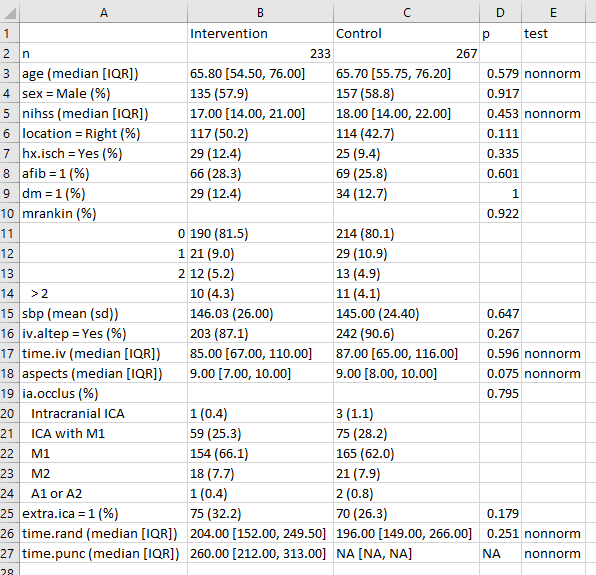
\includegraphics[width=0.9\linewidth]{images/fs-table1inExcel}

And from here, I can either drop it directly into Word, or present it as
is, or start tweaking it to meet formatting needs.

\subsection{Approach B: Produce the Table so you can cut and paste
it}\label{approach-b-produce-the-table-so-you-can-cut-and-paste-it}

\begin{Shaded}
\begin{Highlighting}[]
\KeywordTok{print}\NormalTok{(att2, }
      \DataTypeTok{nonnormal =} \KeywordTok{c}\NormalTok{(}\StringTok{"age"}\NormalTok{, }\StringTok{"nihss"}\NormalTok{, }\StringTok{"time.iv"}\NormalTok{, }\StringTok{"aspects"}\NormalTok{, }\StringTok{"time.rand"}\NormalTok{),}
      \DataTypeTok{exact =} \KeywordTok{c}\NormalTok{(}\StringTok{"location"}\NormalTok{, }\StringTok{"mrankin"}\NormalTok{),}
      \DataTypeTok{quote =} \OtherTok{TRUE}\NormalTok{, }\DataTypeTok{noSpaces =} \OtherTok{TRUE}\NormalTok{)}
\end{Highlighting}
\end{Shaded}

This will look like a mess by itself, but if you:

\begin{enumerate}
\def\labelenumi{\arabic{enumi}.}
\tightlist
\item
  copy and paste that mess into Excel
\item
  select Text to Columns from the Data menu
\item
  select Delimited, then Space and select Treat consecutive delimiters
  as one
\end{enumerate}

you should get something usable again.

Or, in Word,

\begin{enumerate}
\def\labelenumi{\arabic{enumi}.}
\tightlist
\item
  insert the text
\item
  select the text with your mouse
\item
  select Insert \ldots{} Table \ldots{} Convert Text to Table
\item
  place a quotation mark in the ``Other'' area under Separate text at
  \ldots{}
\end{enumerate}

After dropping blank columns, the result looks pretty good.

\section{A Controlled Biological Experiment - The Blood-Brain
Barrier}\label{a-controlled-biological-experiment---the-blood-brain-barrier}

My source for the data and the following explanatory paragraph is page
307 from \citet{RamseySchafer2002}. The original data come from
\citet{Barnett1995}.

\begin{quote}
The human brain (and that of rats, coincidentally) is protected from the
bacteria and toxins that course through the bloodstream by something
called the blood-brain barrier. After a method of disrupting the barrier
was developed, researchers tested this new mechanism, as follows. A
series of 34 rats were inoculated with human lung cancer cells to induce
brain tumors. After 9-11 days they were infused with either the barrier
disruption (BD) solution or, as a control, a normal saline (NS)
solution. Fifteen minutes later, the rats received a standard dose of a
particular therapeutic antibody (L6-F(ab')2. The key measure of the
effectiveness of transmission across the brain-blood barrier is the
ratio of the antibody concentration in the brain tumor to the antibody
concentration in normal tissue outside the brain. The rats were then
sacrificed, and the amounts of antibody in the brain tumor and in normal
tissue from the liver were measured. The study's primary objective is to
determine whether the antibody concentration in the tumor increased when
the blood-barrier disruption infusion was given, and if so, by how much?
\end{quote}

\section{\texorpdfstring{The \texttt{bloodbrain.csv}
file}{The bloodbrain.csv file}}\label{the-bloodbrain.csv-file}

Consider the data, available on the Data and Code page of
\href{https://github.com/THOMASELOVE/432-2018}{our course website} in
the \texttt{bloodbrain.csv} file, which includes the following
variables:

\begin{longtable}[]{@{}rl@{}}
\toprule
\begin{minipage}[b]{0.12\columnwidth}\raggedleft\strut
Variable\strut
\end{minipage} & \begin{minipage}[b]{0.59\columnwidth}\raggedright\strut
Description\strut
\end{minipage}\tabularnewline
\midrule
\endhead
\begin{minipage}[t]{0.12\columnwidth}\raggedleft\strut
\texttt{case}\strut
\end{minipage} & \begin{minipage}[t]{0.59\columnwidth}\raggedright\strut
identification number for the rat (1 - 34)\strut
\end{minipage}\tabularnewline
\begin{minipage}[t]{0.12\columnwidth}\raggedleft\strut
\texttt{brain}\strut
\end{minipage} & \begin{minipage}[t]{0.59\columnwidth}\raggedright\strut
an outcome: Brain tumor antibody count (per gram)\strut
\end{minipage}\tabularnewline
\begin{minipage}[t]{0.12\columnwidth}\raggedleft\strut
\texttt{liver}\strut
\end{minipage} & \begin{minipage}[t]{0.59\columnwidth}\raggedright\strut
an outcome: Liver antibody count (per gram)\strut
\end{minipage}\tabularnewline
\begin{minipage}[t]{0.12\columnwidth}\raggedleft\strut
\texttt{tlratio}\strut
\end{minipage} & \begin{minipage}[t]{0.59\columnwidth}\raggedright\strut
an outcome: tumor / liver concentration ratio\strut
\end{minipage}\tabularnewline
\begin{minipage}[t]{0.12\columnwidth}\raggedleft\strut
\texttt{solution}\strut
\end{minipage} & \begin{minipage}[t]{0.59\columnwidth}\raggedright\strut
the treatment: BD (barrier disruption) or NS (normal saline)\strut
\end{minipage}\tabularnewline
\begin{minipage}[t]{0.12\columnwidth}\raggedleft\strut
\texttt{sactime}\strut
\end{minipage} & \begin{minipage}[t]{0.59\columnwidth}\raggedright\strut
a design variable: Sacrifice time (hours; either 0.5, 3, 24 or 72)\strut
\end{minipage}\tabularnewline
\begin{minipage}[t]{0.12\columnwidth}\raggedleft\strut
\texttt{postin}\strut
\end{minipage} & \begin{minipage}[t]{0.59\columnwidth}\raggedright\strut
covariate: Days post-inoculation of lung cancer cells (9, 10 or
11)\strut
\end{minipage}\tabularnewline
\begin{minipage}[t]{0.12\columnwidth}\raggedleft\strut
\texttt{sex}\strut
\end{minipage} & \begin{minipage}[t]{0.59\columnwidth}\raggedright\strut
covariate: M or F\strut
\end{minipage}\tabularnewline
\begin{minipage}[t]{0.12\columnwidth}\raggedleft\strut
\texttt{wt.init}\strut
\end{minipage} & \begin{minipage}[t]{0.59\columnwidth}\raggedright\strut
covariate: Initial weight (grams)\strut
\end{minipage}\tabularnewline
\begin{minipage}[t]{0.12\columnwidth}\raggedleft\strut
\texttt{wt.loss}\strut
\end{minipage} & \begin{minipage}[t]{0.59\columnwidth}\raggedright\strut
covariate: Weight loss (grams)\strut
\end{minipage}\tabularnewline
\begin{minipage}[t]{0.12\columnwidth}\raggedleft\strut
\texttt{wt.tumor}\strut
\end{minipage} & \begin{minipage}[t]{0.59\columnwidth}\raggedright\strut
covariate: Tumor weight (10\textsuperscript{-4} grams)\strut
\end{minipage}\tabularnewline
\bottomrule
\end{longtable}

And here's what the data look like in R.

\begin{Shaded}
\begin{Highlighting}[]
\NormalTok{bloodbrain}
\end{Highlighting}
\end{Shaded}

\begin{verbatim}
# A tibble: 34 x 11
    case  brain   liver tlratio solution sactime postin sex   wt.init
   <int>  <int>   <int>   <dbl> <fct>      <dbl>  <int> <fct>   <int>
 1     1  41081 1456164  0.0282 BD         0.500     10 F         239
 2     2  44286 1602171  0.0276 BD         0.500     10 F         225
 3     3 102926 1601936  0.0642 BD         0.500     10 F         224
 4     4  25927 1776411  0.0146 BD         0.500     10 F         184
 5     5  42643 1351184  0.0316 BD         0.500     10 F         250
 6     6  31342 1790863  0.0175 NS         0.500     10 F         196
 7     7  22815 1633386  0.0140 NS         0.500     10 F         200
 8     8  16629 1618757  0.0103 NS         0.500     10 F         273
 9     9  22315 1567602  0.0142 NS         0.500     10 F         216
10    10  77961 1060057  0.0735 BD         3.00      10 F         267
# ... with 24 more rows, and 2 more variables: wt.loss <dbl>,
#   wt.tumor <int>
\end{verbatim}

\section{\texorpdfstring{A Table 1 for
\texttt{bloodbrain}}{A Table 1 for bloodbrain}}\label{a-table-1-for-bloodbrain}

\citet{Barnett1995} did not provide a Table 1 for these data, so let's
build one to compare the two \texttt{solutions} (\texttt{BD} vs.
\texttt{NS}) on the covariates and outcomes, plus the natural logarithm
of the tumor/liver concentration ratio (\texttt{tlratio}). We'll opt to
treat the sacrifice time (\texttt{sactime}) and the days
post-inoculation of lung cancer cells (\texttt{postin}) as categorical
rather than quantitative variables.

\begin{Shaded}
\begin{Highlighting}[]
\NormalTok{bloodbrain <-}\StringTok{ }\NormalTok{bloodbrain }\OperatorTok
\StringTok{    }\KeywordTok{mutate}\NormalTok{(}\DataTypeTok{logTL =} \KeywordTok{log}\NormalTok{(tlratio))}

\KeywordTok{dput}\NormalTok{(}\KeywordTok{names}\NormalTok{(bloodbrain))}
\end{Highlighting}
\end{Shaded}

\begin{verbatim}
c("case", "brain", "liver", "tlratio", "solution", "sactime", 
"postin", "sex", "wt.init", "wt.loss", "wt.tumor", "logTL")
\end{verbatim}

OK - there's the list of variables we'll need. I'll put the outcomes at
the bottom of the table.

\begin{Shaded}
\begin{Highlighting}[]
\NormalTok{bb.vars <-}\StringTok{ }\KeywordTok{c}\NormalTok{(}\StringTok{"sactime"}\NormalTok{, }\StringTok{"postin"}\NormalTok{, }\StringTok{"sex"}\NormalTok{, }\StringTok{"wt.init"}\NormalTok{, }\StringTok{"wt.loss"}\NormalTok{, }
             \StringTok{"wt.tumor"}\NormalTok{, }\StringTok{"brain"}\NormalTok{, }\StringTok{"liver"}\NormalTok{, }\StringTok{"tlratio"}\NormalTok{, }\StringTok{"logTL"}\NormalTok{)}

\NormalTok{bb.factors <-}\StringTok{ }\KeywordTok{c}\NormalTok{(}\StringTok{"sactime"}\NormalTok{, }\StringTok{"sex"}\NormalTok{, }\StringTok{"postin"}\NormalTok{)}

\NormalTok{bb.att1 <-}\StringTok{ }\KeywordTok{CreateTableOne}\NormalTok{(}\DataTypeTok{data =}\NormalTok{ bloodbrain,}
                          \DataTypeTok{vars =}\NormalTok{ bb.vars,}
                          \DataTypeTok{factorVars =}\NormalTok{ bb.factors,}
                          \DataTypeTok{strata =} \KeywordTok{c}\NormalTok{(}\StringTok{"solution"}\NormalTok{))}
\KeywordTok{summary}\NormalTok{(bb.att1)}
\end{Highlighting}
\end{Shaded}

\begin{verbatim}

     ### Summary of continuous variables ###

solution: BD
          n miss p.miss   mean    sd median    p25   p75    min   max
wt.init  17    0      0    243 3e+01  2e+02  2e+02 3e+02  2e+02 3e+02
wt.loss  17    0      0      3 5e+00  4e+00  1e+00 6e+00 -5e+00 1e+01
wt.tumor 17    0      0    157 8e+01  2e+02  1e+02 2e+02  2e+01 4e+02
brain    17    0      0  56043 3e+04  5e+04  4e+04 8e+04  6e+03 1e+05
liver    17    0      0 672577 7e+05  6e+05  2e+04 1e+06  2e+03 2e+06
tlratio  17    0      0      2 3e+00  1e-01  6e-02 3e+00  1e-02 9e+00
logTL    17    0      0     -1 2e+00 -2e+00 -3e+00 1e+00 -4e+00 2e+00
          skew kurt
wt.init  -0.39  0.7
wt.loss  -0.10  0.2
wt.tumor  0.53  1.0
brain     0.29 -0.6
liver     0.35 -1.7
tlratio   1.58  1.7
logTL     0.08 -1.7
-------------------------------------------------------- 
solution: NS
          n miss p.miss   mean    sd median    p25    p75    min   max
wt.init  17    0      0    240 3e+01  2e+02  2e+02  3e+02  2e+02 3e+02
wt.loss  17    0      0      4 4e+00  3e+00  2e+00  7e+00 -4e+00 1e+01
wt.tumor 17    0      0    209 1e+02  2e+02  2e+02  3e+02  3e+01 5e+02
brain    17    0      0  23887 1e+04  2e+04  1e+04  3e+04  1e+03 5e+04
liver    17    0      0 664975 7e+05  7e+05  2e+04  1e+06  9e+02 2e+06
tlratio  17    0      0      1 2e+00  5e-02  3e-02  9e-01  1e-02 7e+00
logTL    17    0      0     -2 2e+00 -3e+00 -3e+00 -7e-02 -5e+00 2e+00
          skew  kurt
wt.init   0.33 -0.48
wt.loss  -0.09  0.08
wt.tumor  0.63  0.77
brain     0.30 -0.35
liver     0.40 -1.56
tlratio   2.27  4.84
logTL     0.27 -1.61

p-values
             pNormal  pNonNormal
wt.init  0.807308940 0.641940278
wt.loss  0.683756156 0.876749808
wt.tumor 0.151510151 0.190482094
brain    0.001027678 0.002579901
liver    0.974853609 0.904045603
tlratio  0.320501715 0.221425879
logTL    0.351633525 0.221425879

Standardize mean differences
             1 vs 2
wt.init  0.08435244
wt.loss  0.14099823
wt.tumor 0.50397184
brain    1.23884159
liver    0.01089667
tlratio  0.34611465
logTL    0.32420504

=======================================================================================

     ### Summary of categorical variables ### 

solution: BD
     var  n miss p.miss level freq percent cum.percent
 sactime 17    0    0.0   0.5    5    29.4        29.4
                            3    4    23.5        52.9
                           24    4    23.5        76.5
                           72    4    23.5       100.0
                                                      
  postin 17    0    0.0     9    1     5.9         5.9
                           10   14    82.4        88.2
                           11    2    11.8       100.0
                                                      
     sex 17    0    0.0     F   13    76.5        76.5
                            M    4    23.5       100.0
                                                      
-------------------------------------------------------- 
solution: NS
     var  n miss p.miss level freq percent cum.percent
 sactime 17    0    0.0   0.5    4    23.5        23.5
                            3    5    29.4        52.9
                           24    4    23.5        76.5
                           72    4    23.5       100.0
                                                      
  postin 17    0    0.0     9    2    11.8        11.8
                           10   13    76.5        88.2
                           11    2    11.8       100.0
                                                      
     sex 17    0    0.0     F   13    76.5        76.5
                            M    4    23.5       100.0
                                                      

p-values
          pApprox pExact
sactime 0.9739246      1
postin  0.8309504      1
sex     1.0000000      1

Standardize mean differences
           1 vs 2
sactime 0.1622214
postin  0.2098877
sex     0.0000000
\end{verbatim}

Note that, in this particular case, the decisions we make about
normality vs.~non-normality (for quantitative variables) and the
decisions we make about approximate vs.~exact testing (for categorical
variables) won't actually change the implications of the \emph{p}
values. Each approach gives similar results for each variable. Of
course, that's not always true.

\subsection{\texorpdfstring{Generate final Table 1 for
\texttt{bloodbrain}}{Generate final Table 1 for bloodbrain}}\label{generate-final-table-1-for-bloodbrain}

I'll choose to treat \texttt{tlratio} and its logarithm as non-Normal,
but otherwise, use t tests, but admittedly, that's an arbitrary
decision, really.

\begin{Shaded}
\begin{Highlighting}[]
\KeywordTok{print}\NormalTok{(bb.att1, }\DataTypeTok{nonnormal =} \KeywordTok{c}\NormalTok{(}\StringTok{"tlratio"}\NormalTok{, }\StringTok{"logTL"}\NormalTok{))}
\end{Highlighting}
\end{Shaded}

\begin{verbatim}
                        Stratified by solution
                         BD                      NS                      
  n                             17                      17               
  sactime (%)                                                            
     0.5                         5 (29.4)                4 (23.5)        
     3                           4 (23.5)                5 (29.4)        
     24                          4 (23.5)                4 (23.5)        
     72                          4 (23.5)                4 (23.5)        
  postin (%)                                                             
     9                           1 ( 5.9)                2 (11.8)        
     10                         14 (82.4)               13 (76.5)        
     11                          2 (11.8)                2 (11.8)        
  sex = M (%)                    4 (23.5)                4 (23.5)        
  wt.init (mean (sd))       242.82 (27.23)          240.47 (28.54)       
  wt.loss (mean (sd))         3.34 (4.68)             3.94 (3.88)        
  wt.tumor (mean (sd))      157.29 (84.00)          208.53 (116.68)      
  brain (mean (sd))       56043.41 (33675.40)     23887.18 (14610.53)    
  liver (mean (sd))      672577.35 (694479.58)   664975.47 (700773.13)   
  tlratio (median [IQR])      0.12 [0.06, 2.84]       0.05 [0.03, 0.94]  
  logTL (median [IQR])       -2.10 [-2.74, 1.04]     -2.95 [-3.41, -0.07]
                        Stratified by solution
                         p      test   
  n                                    
  sactime (%)             0.974        
     0.5                               
     3                                 
     24                                
     72                                
  postin (%)              0.831        
     9                                 
     10                                
     11                                
  sex = M (%)             1.000        
  wt.init (mean (sd))     0.807        
  wt.loss (mean (sd))     0.684        
  wt.tumor (mean (sd))    0.152        
  brain (mean (sd))       0.001        
  liver (mean (sd))       0.975        
  tlratio (median [IQR])  0.221 nonnorm
  logTL (median [IQR])    0.221 nonnorm
\end{verbatim}

Or, we can get an Excel-readable version placed in a \texttt{data}
subfolder, using

\begin{Shaded}
\begin{Highlighting}[]
\NormalTok{bb.t1 <-}\StringTok{ }\KeywordTok{print}\NormalTok{(bb.att1, }\DataTypeTok{nonnormal =} \KeywordTok{c}\NormalTok{(}\StringTok{"tlratio"}\NormalTok{, }\StringTok{"logTL"}\NormalTok{), }\DataTypeTok{quote =} \OtherTok{FALSE}\NormalTok{,}
               \DataTypeTok{noSpaces =} \OtherTok{TRUE}\NormalTok{, }\DataTypeTok{printToggle =} \OtherTok{FALSE}\NormalTok{)}

\KeywordTok{write.csv}\NormalTok{(bb.t1, }\DataTypeTok{file =} \StringTok{"data/bb-table1.csv"}\NormalTok{)}
\end{Highlighting}
\end{Shaded}

which, when dropped into Excel, will look like this:

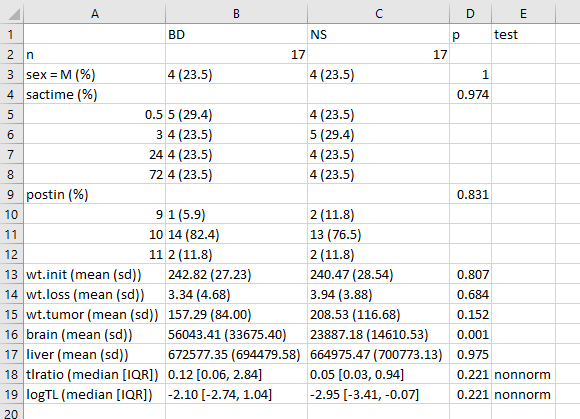
\includegraphics[width=0.9\linewidth]{images/bb-table1inExcel}

One thing I would definitely clean up here, in practice, is to change
the presentation of the \emph{p} value for \texttt{sex} from 1 to
\textgreater{} 0.99, or just omit it altogether. I'd also drop the
\texttt{computer-ese} where possible, add units for the measures, round
\textbf{a lot}, identify the outcomes carefully, and use notes to
indicate deviations from the main approach.

\subsection{A More Finished Version (after Cleanup in
Word)}\label{a-more-finished-version-after-cleanup-in-word}

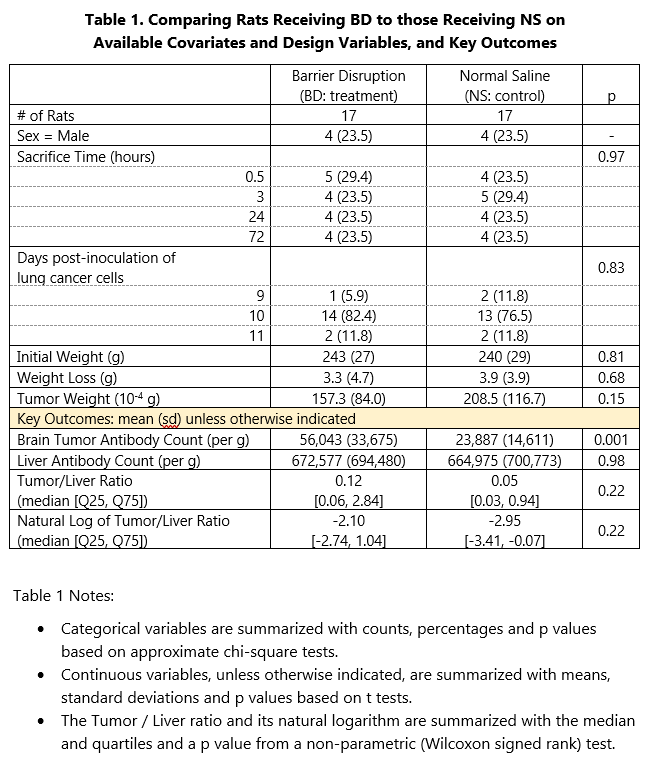
\includegraphics[width=0.95\linewidth]{images/bb-table1inWord}

\chapter{Linear Regression on a small SMART data
set}\label{linear-regression-on-a-small-smart-data-set}

\section{BRFSS and SMART}\label{brfss-and-smart}

The Centers for Disease Control analyzes Behavioral Risk Factor
Surveillance System (BRFSS) survey data for specific metropolitan and
micropolitan statistical areas (MMSAs) in a program called the
\href{https://www.cdc.gov/brfss/smart/Smart_data.htm}{Selected
Metropolitan/Micropolitan Area Risk Trends of BRFSS} (SMART BRFSS.)

In this work, we will focus on
\href{https://www.cdc.gov/brfss/smart/smart_2016.html}{data from the
2016 SMART}, and in particular on data from the Cleveland-Elyria, OH,
Metropolitan Statistical Area. The purpose of this survey is to provide
localized health information that can help public health practitioners
identify local emerging health problems, plan and evaluate local
responses, and efficiently allocate resources to specific needs.

\subsection{Key resources}\label{key-resources}

\begin{itemize}
\tightlist
\item
  the full data are available in the form of the 2016 SMART BRFSS MMSA
  Data, found in a zipped
  \href{https://www.cdc.gov/brfss/smart/2016/MMSA2016_XPT.zip}{SAS
  Transport Format} file. The data were released in August 2017.
\item
  the
  \href{https://www.cdc.gov/brfss/smart/2016/mmsa_varlayout_16.pdf}{MMSA
  Variable Layout PDF} which simply lists the variables included in the
  data file
\item
  the
  \href{https://www.cdc.gov/brfss/annual_data/2016/pdf/2016_calculated_variables_version4.pdf}{Calculated
  Variables PDF} which describes the risk factors by data variable names
  - there is also an
  \href{https://www.cdc.gov/brfss/annual_data/2016/Summary_Matrix_16.html}{online
  summary matrix of these calculated variables}, as well.
\item
  the lengthy
  \href{https://www.cdc.gov/brfss/questionnaires/pdf-ques/2016_BRFSS_Questionnaire_FINAL.pdf}{2016
  Survey Questions PDF} which lists all questions asked as part of the
  BRFSS in 2016
\item
  the enormous
  \href{https://www.cdc.gov/brfss/annual_data/2016/pdf/codebook16_llcp.pdf}{Codebook
  for the 2016 BRFSS Survey PDF} which identifies the variables by name
  for us.
\end{itemize}

Later this term, we'll use all of those resources to help construct a
more complete data set than we'll study today. I'll also demonstrate how
I built the \texttt{smartcle1} data set that we'll use in this Chapter.

\section{\texorpdfstring{The \texttt{smartcle1} data:
Cookbook}{The smartcle1 data: Cookbook}}\label{the-smartcle1-data-cookbook}

The \texttt{smartcle1.csv} data file available on the Data and Code page
of \href{https://github.com/THOMASELOVE/432-2018}{our website} describes
information on 11 variables for 1036 respondents to the BRFSS 2016, who
live in the Cleveland-Elyria, OH, Metropolitan Statistical Area. The
variables in the \texttt{smartcle1.csv} file are listed below, along
with (in some cases) the BRFSS items that generate these responses.

\begin{longtable}[]{@{}rl@{}}
\toprule
\begin{minipage}[b]{0.14\columnwidth}\raggedleft\strut
Variable\strut
\end{minipage} & \begin{minipage}[b]{0.74\columnwidth}\raggedright\strut
Description\strut
\end{minipage}\tabularnewline
\midrule
\endhead
\begin{minipage}[t]{0.14\columnwidth}\raggedleft\strut
\texttt{SEQNO}\strut
\end{minipage} & \begin{minipage}[t]{0.74\columnwidth}\raggedright\strut
respondent identification number (all begin with 2016)\strut
\end{minipage}\tabularnewline
\begin{minipage}[t]{0.14\columnwidth}\raggedleft\strut
\texttt{physhealth}\strut
\end{minipage} & \begin{minipage}[t]{0.74\columnwidth}\raggedright\strut
Now thinking about your physical health, which includes physical illness
and injury, for how many days during the past 30 days was your physical
health not good?\strut
\end{minipage}\tabularnewline
\begin{minipage}[t]{0.14\columnwidth}\raggedleft\strut
\texttt{menthealth}\strut
\end{minipage} & \begin{minipage}[t]{0.74\columnwidth}\raggedright\strut
Now thinking about your mental health, which includes stress,
depression, and problems with emotions, for how many days during the
past 30 days was your mental health not good?\strut
\end{minipage}\tabularnewline
\begin{minipage}[t]{0.14\columnwidth}\raggedleft\strut
\texttt{poorhealth}\strut
\end{minipage} & \begin{minipage}[t]{0.74\columnwidth}\raggedright\strut
During the past 30 days, for about how many days did poor physical or
mental health keep you from doing your usual activities, such as
self-care, work, or recreation?\strut
\end{minipage}\tabularnewline
\begin{minipage}[t]{0.14\columnwidth}\raggedleft\strut
\texttt{genhealth}\strut
\end{minipage} & \begin{minipage}[t]{0.74\columnwidth}\raggedright\strut
Would you say that in general, your health is \ldots{} (five categories:
Excellent, Very Good, Good, Fair or Poor)\strut
\end{minipage}\tabularnewline
\begin{minipage}[t]{0.14\columnwidth}\raggedleft\strut
\texttt{bmi}\strut
\end{minipage} & \begin{minipage}[t]{0.74\columnwidth}\raggedright\strut
Body mass index, in kg/m\textsuperscript{2}\strut
\end{minipage}\tabularnewline
\begin{minipage}[t]{0.14\columnwidth}\raggedleft\strut
\texttt{female}\strut
\end{minipage} & \begin{minipage}[t]{0.74\columnwidth}\raggedright\strut
Sex, 1 = female, 0 = male\strut
\end{minipage}\tabularnewline
\begin{minipage}[t]{0.14\columnwidth}\raggedleft\strut
\texttt{internet30}\strut
\end{minipage} & \begin{minipage}[t]{0.74\columnwidth}\raggedright\strut
Have you used the internet in the past 30 days? (1 = yes, 0 = no)\strut
\end{minipage}\tabularnewline
\begin{minipage}[t]{0.14\columnwidth}\raggedleft\strut
\texttt{exerany}\strut
\end{minipage} & \begin{minipage}[t]{0.74\columnwidth}\raggedright\strut
During the past month, other than your regular job, did you participate
in any physical activities or exercises such as running, calisthenics,
golf, gardening, or walking for exercise? (1 = yes, 0 = no)\strut
\end{minipage}\tabularnewline
\begin{minipage}[t]{0.14\columnwidth}\raggedleft\strut
\texttt{sleephrs}\strut
\end{minipage} & \begin{minipage}[t]{0.74\columnwidth}\raggedright\strut
On average, how many hours of sleep do you get in a 24-hour
period?\strut
\end{minipage}\tabularnewline
\begin{minipage}[t]{0.14\columnwidth}\raggedleft\strut
\texttt{alcdays}\strut
\end{minipage} & \begin{minipage}[t]{0.74\columnwidth}\raggedright\strut
How many days during the past 30 days did you have at least one drink of
any alcoholic beverage such as beer, wine, a malt beverage or
liquor?\strut
\end{minipage}\tabularnewline
\bottomrule
\end{longtable}

\begin{Shaded}
\begin{Highlighting}[]
\KeywordTok{str}\NormalTok{(smartcle1)}
\end{Highlighting}
\end{Shaded}

\begin{verbatim}
Classes 'tbl_df', 'tbl' and 'data.frame':   1036 obs. of  11 variables:
 $ SEQNO     : num  2.02e+09 2.02e+09 2.02e+09 2.02e+09 2.02e+09 ...
 $ physhealth: int  0 0 1 0 5 4 2 2 0 0 ...
 $ menthealth: int  0 0 5 0 0 18 0 3 0 0 ...
 $ poorhealth: int  NA NA 0 NA 0 6 0 0 NA NA ...
 $ genhealth : Factor w/ 5 levels "1_Excellent",..: 2 1 2 3 1 2 3 3 2 3 ...
 $ bmi       : num  26.7 23.7 26.9 21.7 24.1 ...
 $ female    : int  1 0 0 1 0 0 1 1 0 0 ...
 $ internet30: int  1 1 1 1 1 1 1 1 1 1 ...
 $ exerany   : int  1 1 0 1 1 1 1 1 1 0 ...
 $ sleephrs  : int  6 6 8 9 7 5 9 7 7 7 ...
 $ alcdays   : int  1 4 4 3 2 28 4 2 4 25 ...
\end{verbatim}

\section{\texorpdfstring{\texttt{smartcle2}: Omitting Missing
Observations: Complete-Case
Analyses}{smartcle2: Omitting Missing Observations: Complete-Case Analyses}}\label{smartcle2-omitting-missing-observations-complete-case-analyses}

For the purpose of fitting our first few models, we will eliminate the
missingness problem, and look only at the \emph{complete cases} in our
\texttt{smartcle1} data. We will discuss methods for imputing missing
data later in these Notes.

To inspect the missingness in our data, we might consider using the
\texttt{skim} function from the \texttt{skimr} package. We'll exclude
the respondent identifier code (\texttt{SEQNO}) from this summary as
uninteresting.

\begin{Shaded}
\begin{Highlighting}[]
\KeywordTok{skim_with}\NormalTok{(}\DataTypeTok{numeric =} \KeywordTok{list}\NormalTok{(}\DataTypeTok{hist =} \OtherTok{NULL}\NormalTok{), }\DataTypeTok{integer =} \KeywordTok{list}\NormalTok{(}\DataTypeTok{hist =} \OtherTok{NULL}\NormalTok{))}
\NormalTok{## above line eliminates the sparkline histograms}
\NormalTok{## it can be commented out when working in the console,}
\NormalTok{## but I need it to produce the Notes without errors right now}

\NormalTok{smartcle1 }\OperatorTok\StringTok{ }
\StringTok{    }\KeywordTok{skim}\NormalTok{(}\OperatorTok{-}\NormalTok{SEQNO)}
\end{Highlighting}
\end{Shaded}

\begin{verbatim}
Skim summary statistics
 n obs: 1036 
 n variables: 11 

Variable type: factor 
  variable missing complete    n n_unique
 genhealth       3     1033 1036        5
                             top_counts ordered
 2_V: 350, 3_G: 344, 1_E: 173, 4_F: 122   FALSE

Variable type: integer 
   variable missing complete    n mean   sd p0 p25 median p75 p100
    alcdays      46      990 1036 4.65 8.05  0   0      1   4   30
    exerany       3     1033 1036 0.76 0.43  0   1      1   1    1
     female       0     1036 1036 0.6  0.49  0   0      1   1    1
 internet30       6     1030 1036 0.81 0.39  0   1      1   1    1
 menthealth      11     1025 1036 2.72 6.82  0   0      0   2   30
 physhealth      17     1019 1036 3.97 8.67  0   0      0   2   30
 poorhealth     543      493 1036 4.07 8.09  0   0      0   3   30
   sleephrs       8     1028 1036 7.02 1.53  1   6      7   8   20

Variable type: numeric 
 variable missing complete    n  mean   sd    p0  p25 median   p75  p100
      bmi      84      952 1036 27.89 6.47 12.71 23.7  26.68 30.53 66.06
\end{verbatim}

Now, we'll create a new tibble called \texttt{smartcle2} which contains
every variable except \texttt{poorhealth}, and which includes all
respondents with complete data on the variables (other than
\texttt{poorhealth}). We'll store those observations with complete data
in the \texttt{smartcle2} tibble.

\begin{Shaded}
\begin{Highlighting}[]
\NormalTok{smartcle2 <-}\StringTok{ }\NormalTok{smartcle1 }\OperatorTok\StringTok{ }
\StringTok{    }\KeywordTok{select}\NormalTok{(}\OperatorTok{-}\NormalTok{poorhealth) }\OperatorTok
\StringTok{    }\KeywordTok{filter}\NormalTok{(}\KeywordTok{complete.cases}\NormalTok{(.))}

\NormalTok{smartcle2}
\end{Highlighting}
\end{Shaded}

\begin{verbatim}
# A tibble: 896 x 10
     SEQNO physhealth menthealth genhealth   bmi female internet30 exerany
     <dbl>      <int>      <int> <fct>     <dbl>  <int>      <int>   <int>
 1  2.02e9          0          0 2_VeryGo~  26.7      1          1       1
 2  2.02e9          0          0 1_Excell~  23.7      0          1       1
 3  2.02e9          1          5 2_VeryGo~  26.9      0          1       0
 4  2.02e9          0          0 3_Good     21.7      1          1       1
 5  2.02e9          5          0 1_Excell~  24.1      0          1       1
 6  2.02e9          4         18 2_VeryGo~  27.6      0          1       1
 7  2.02e9          2          0 3_Good     25.7      1          1       1
 8  2.02e9          2          3 3_Good     28.5      1          1       1
 9  2.02e9          0          0 2_VeryGo~  28.6      0          1       1
10  2.02e9          0          0 3_Good     23.1      0          1       0
# ... with 886 more rows, and 2 more variables: sleephrs <int>,
#   alcdays <int>
\end{verbatim}

Note that there are only 896 respondents with \textbf{complete} data on
the 10 variables (excluding \texttt{poorhealth}) in the
\texttt{smartcle2} tibble, as compared to our original
\texttt{smartcle1} data which described 1036 respondents and 11
variables, but with lots of missing data.

\section{\texorpdfstring{Summarizing the \texttt{smartcle2} data
numerically}{Summarizing the smartcle2 data numerically}}\label{summarizing-the-smartcle2-data-numerically}

\subsection{\texorpdfstring{The New Toy: The \texttt{skim}
function}{The New Toy: The skim function}}\label{the-new-toy-the-skim-function}

\begin{Shaded}
\begin{Highlighting}[]
\KeywordTok{skim}\NormalTok{(smartcle2, }\OperatorTok{-}\NormalTok{SEQNO)}
\end{Highlighting}
\end{Shaded}

\begin{verbatim}
Skim summary statistics
 n obs: 896 
 n variables: 10 

Variable type: factor 
  variable missing complete   n n_unique
 genhealth       0      896 896        5
                             top_counts ordered
 2_V: 306, 3_G: 295, 1_E: 155, 4_F: 102   FALSE

Variable type: integer 
   variable missing complete   n mean   sd p0 p25 median p75 p100
    alcdays       0      896 896 4.83 8.14  0   0      1   5   30
    exerany       0      896 896 0.77 0.42  0   1      1   1    1
     female       0      896 896 0.58 0.49  0   0      1   1    1
 internet30       0      896 896 0.81 0.39  0   1      1   1    1
 menthealth       0      896 896 2.69 6.72  0   0      0   2   30
 physhealth       0      896 896 3.99 8.64  0   0      0   2   30
   sleephrs       0      896 896 7.02 1.48  1   6      7   8   20

Variable type: numeric 
 variable missing complete   n  mean   sd    p0  p25 median   p75  p100
      bmi       0      896 896 27.87 6.33 12.71 23.7   26.8 30.53 66.06
\end{verbatim}

\subsection{\texorpdfstring{The usual \texttt{summary} for a data
frame}{The usual summary for a data frame}}\label{the-usual-summary-for-a-data-frame}

Of course, we can use the usual \texttt{summary} to get some basic
information about the data.

\begin{Shaded}
\begin{Highlighting}[]
\KeywordTok{summary}\NormalTok{(smartcle2)}
\end{Highlighting}
\end{Shaded}

\begin{verbatim}
     SEQNO             physhealth      menthealth           genhealth  
 Min.   :2.016e+09   Min.   : 0.00   Min.   : 0.000   1_Excellent:155  
 1st Qu.:2.016e+09   1st Qu.: 0.00   1st Qu.: 0.000   2_VeryGood :306  
 Median :2.016e+09   Median : 0.00   Median : 0.000   3_Good     :295  
 Mean   :2.016e+09   Mean   : 3.99   Mean   : 2.693   4_Fair     :102  
 3rd Qu.:2.016e+09   3rd Qu.: 2.00   3rd Qu.: 2.000   5_Poor     : 38  
 Max.   :2.016e+09   Max.   :30.00   Max.   :30.000                    
      bmi            female         internet30        exerany      
 Min.   :12.71   Min.   :0.0000   Min.   :0.0000   Min.   :0.0000  
 1st Qu.:23.70   1st Qu.:0.0000   1st Qu.:1.0000   1st Qu.:1.0000  
 Median :26.80   Median :1.0000   Median :1.0000   Median :1.0000  
 Mean   :27.87   Mean   :0.5848   Mean   :0.8147   Mean   :0.7667  
 3rd Qu.:30.53   3rd Qu.:1.0000   3rd Qu.:1.0000   3rd Qu.:1.0000  
 Max.   :66.06   Max.   :1.0000   Max.   :1.0000   Max.   :1.0000  
    sleephrs         alcdays      
 Min.   : 1.000   Min.   : 0.000  
 1st Qu.: 6.000   1st Qu.: 0.000  
 Median : 7.000   Median : 1.000  
 Mean   : 7.022   Mean   : 4.834  
 3rd Qu.: 8.000   3rd Qu.: 5.000  
 Max.   :20.000   Max.   :30.000  
\end{verbatim}

\subsection{\texorpdfstring{The \texttt{describe} function in
\texttt{Hmisc}}{The describe function in Hmisc}}\label{the-describe-function-in-hmisc}

Or we can use the \texttt{describe} function from the \texttt{Hmisc}
package.

\begin{Shaded}
\begin{Highlighting}[]
\NormalTok{Hmisc}\OperatorTok{::}\KeywordTok{describe}\NormalTok{(}\KeywordTok{select}\NormalTok{(smartcle2, bmi, genhealth, female))}
\end{Highlighting}
\end{Shaded}

\begin{verbatim}
select(smartcle2, bmi, genhealth, female) 

 3  Variables      896  Observations
---------------------------------------------------------------------------
bmi 
       n  missing distinct     Info     Mean      Gmd      .05      .10 
     896        0      467        1    27.87    6.572    20.06    21.23 
     .25      .50      .75      .90      .95 
   23.70    26.80    30.53    35.36    39.30 

lowest : 12.71 13.34 14.72 16.22 17.30, highest: 56.89 57.04 60.95 61.84 66.06
---------------------------------------------------------------------------
genhealth 
       n  missing distinct 
     896        0        5 
                                                                      
Value      1_Excellent  2_VeryGood      3_Good      4_Fair      5_Poor
Frequency          155         306         295         102          38
Proportion       0.173       0.342       0.329       0.114       0.042
---------------------------------------------------------------------------
female 
       n  missing distinct     Info      Sum     Mean      Gmd 
     896        0        2    0.728      524   0.5848   0.4862 

---------------------------------------------------------------------------
\end{verbatim}

\section{Counting as exploratory data
analysis}\label{counting-as-exploratory-data-analysis}

Counting things can be amazingly useful.

\subsection{How many respondents had exercised in the past 30 days? Did
this vary by
sex?}\label{how-many-respondents-had-exercised-in-the-past-30-days-did-this-vary-by-sex}

\begin{Shaded}
\begin{Highlighting}[]
\NormalTok{smartcle2 }\OperatorTok\StringTok{ }\KeywordTok{count}\NormalTok{(female, exerany) }\OperatorTok\StringTok{ }\KeywordTok{mutate}\NormalTok{(}\DataTypeTok{percent =} \DecValTok{100}\OperatorTok{*}\NormalTok{n }\OperatorTok{/}\StringTok{ }\KeywordTok{sum}\NormalTok{(n))}
\end{Highlighting}
\end{Shaded}

\begin{verbatim}
# A tibble: 4 x 4
  female exerany     n percent
   <int>   <int> <int>   <dbl>
1      0       0    64    7.14
2      0       1   308   34.4 
3      1       0   145   16.2 
4      1       1   379   42.3 
\end{verbatim}

so we know now that 42.3\% of the subjects in our data were women who
exercised. Suppose that instead we want to find the percentage of
exercisers within each sex\ldots{}

\begin{Shaded}
\begin{Highlighting}[]
\NormalTok{smartcle2 }\OperatorTok
\StringTok{    }\KeywordTok{count}\NormalTok{(female, exerany) }\OperatorTok
\StringTok{    }\KeywordTok{group_by}\NormalTok{(female) }\OperatorTok
\StringTok{    }\KeywordTok{mutate}\NormalTok{(}\DataTypeTok{prob =} \DecValTok{100}\OperatorTok{*}\NormalTok{n }\OperatorTok{/}\StringTok{ }\KeywordTok{sum}\NormalTok{(n)) }
\end{Highlighting}
\end{Shaded}

\begin{verbatim}
# A tibble: 4 x 4
# Groups:   female [2]
  female exerany     n  prob
   <int>   <int> <int> <dbl>
1      0       0    64  17.2
2      0       1   308  82.8
3      1       0   145  27.7
4      1       1   379  72.3
\end{verbatim}

and now we know that 82.8\% of the males exercised at least once in the
last 30 days, as compared to 72.3\% of the females.

\subsection{\texorpdfstring{What's the distribution of
\texttt{sleephrs}?}{What's the distribution of sleephrs?}}\label{whats-the-distribution-of-sleephrs}

We can count quantitative variables with discrete sets of possible
values, like \texttt{sleephrs}, which is captured as an integer (that
must fall between 0 and 24.)

\begin{Shaded}
\begin{Highlighting}[]
\NormalTok{smartcle2 }\OperatorTok\StringTok{ }\KeywordTok{count}\NormalTok{(sleephrs)}
\end{Highlighting}
\end{Shaded}

\begin{verbatim}
# A tibble: 14 x 2
   sleephrs     n
      <int> <int>
 1        1     5
 2        2     1
 3        3     6
 4        4    20
 5        5    63
 6        6   192
 7        7   276
 8        8   266
 9        9    38
10       10    22
11       11     2
12       12     2
13       16     2
14       20     1
\end{verbatim}

Of course, a natural summary of a quantitative variable like this would
be graphical.

\begin{Shaded}
\begin{Highlighting}[]
\KeywordTok{ggplot}\NormalTok{(smartcle2, }\KeywordTok{aes}\NormalTok{(sleephrs)) }\OperatorTok{+}
\StringTok{    }\KeywordTok{geom_histogram}\NormalTok{(}\DataTypeTok{binwidth =} \DecValTok{1}\NormalTok{, }\DataTypeTok{fill =} \StringTok{"dodgerblue"}\NormalTok{, }\DataTypeTok{col =} \StringTok{"darkred"}\NormalTok{)}
\end{Highlighting}
\end{Shaded}

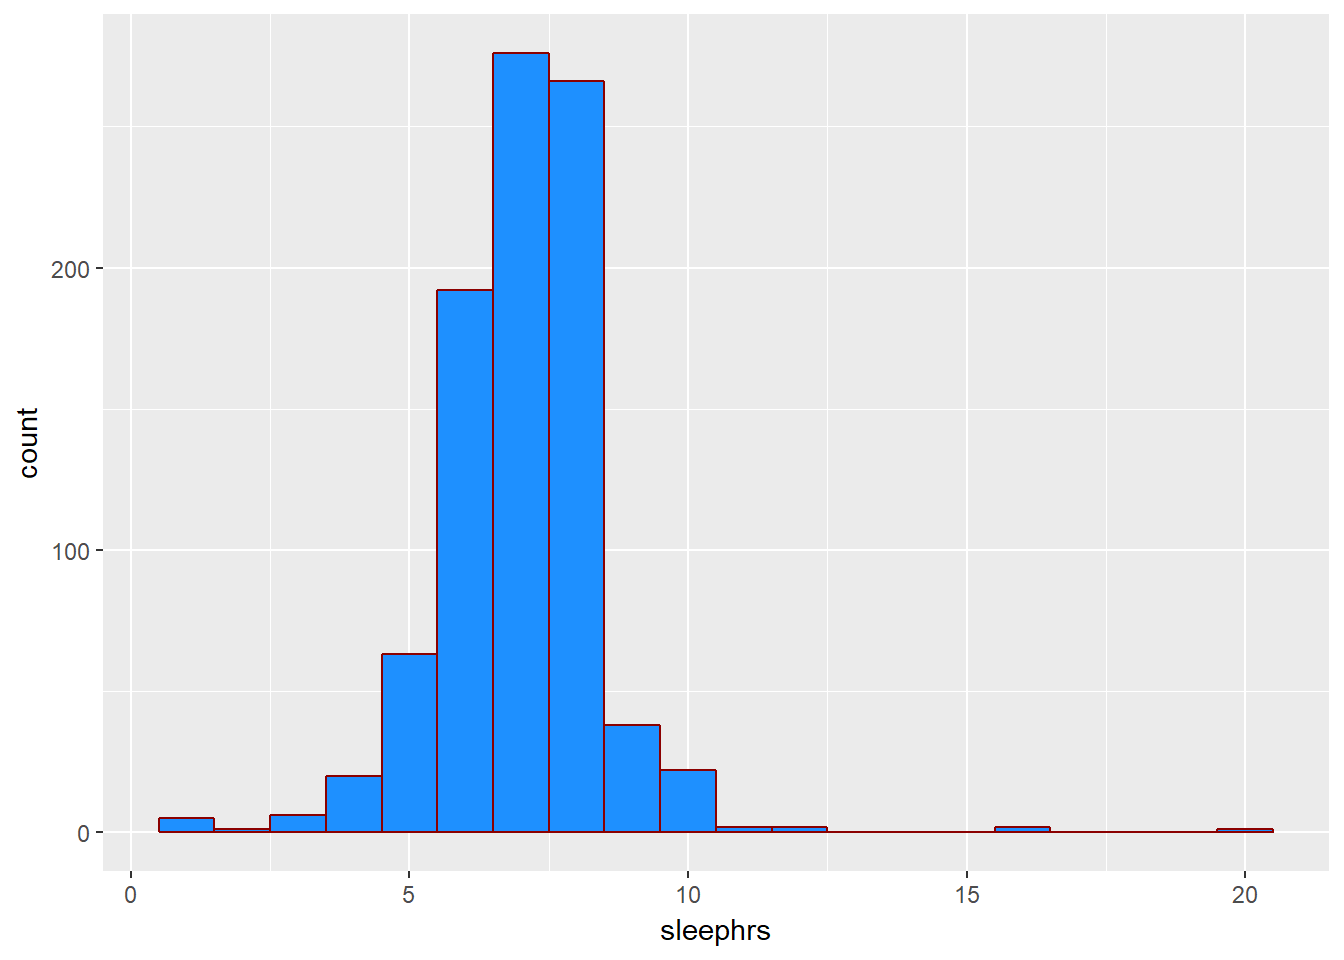
\includegraphics{bookdown-demo_files/figure-latex/c2_histogram_sleephrs_smartcle2-1.pdf}

\subsection{\texorpdfstring{What's the distribution of
\texttt{BMI}?}{What's the distribution of BMI?}}\label{whats-the-distribution-of-bmi}

\begin{Shaded}
\begin{Highlighting}[]
\KeywordTok{ggplot}\NormalTok{(smartcle2, }\KeywordTok{aes}\NormalTok{(bmi)) }\OperatorTok{+}
\StringTok{    }\KeywordTok{geom_histogram}\NormalTok{(}\DataTypeTok{bins =} \DecValTok{30}\NormalTok{, }\DataTypeTok{col =} \StringTok{"white"}\NormalTok{)}
\end{Highlighting}
\end{Shaded}

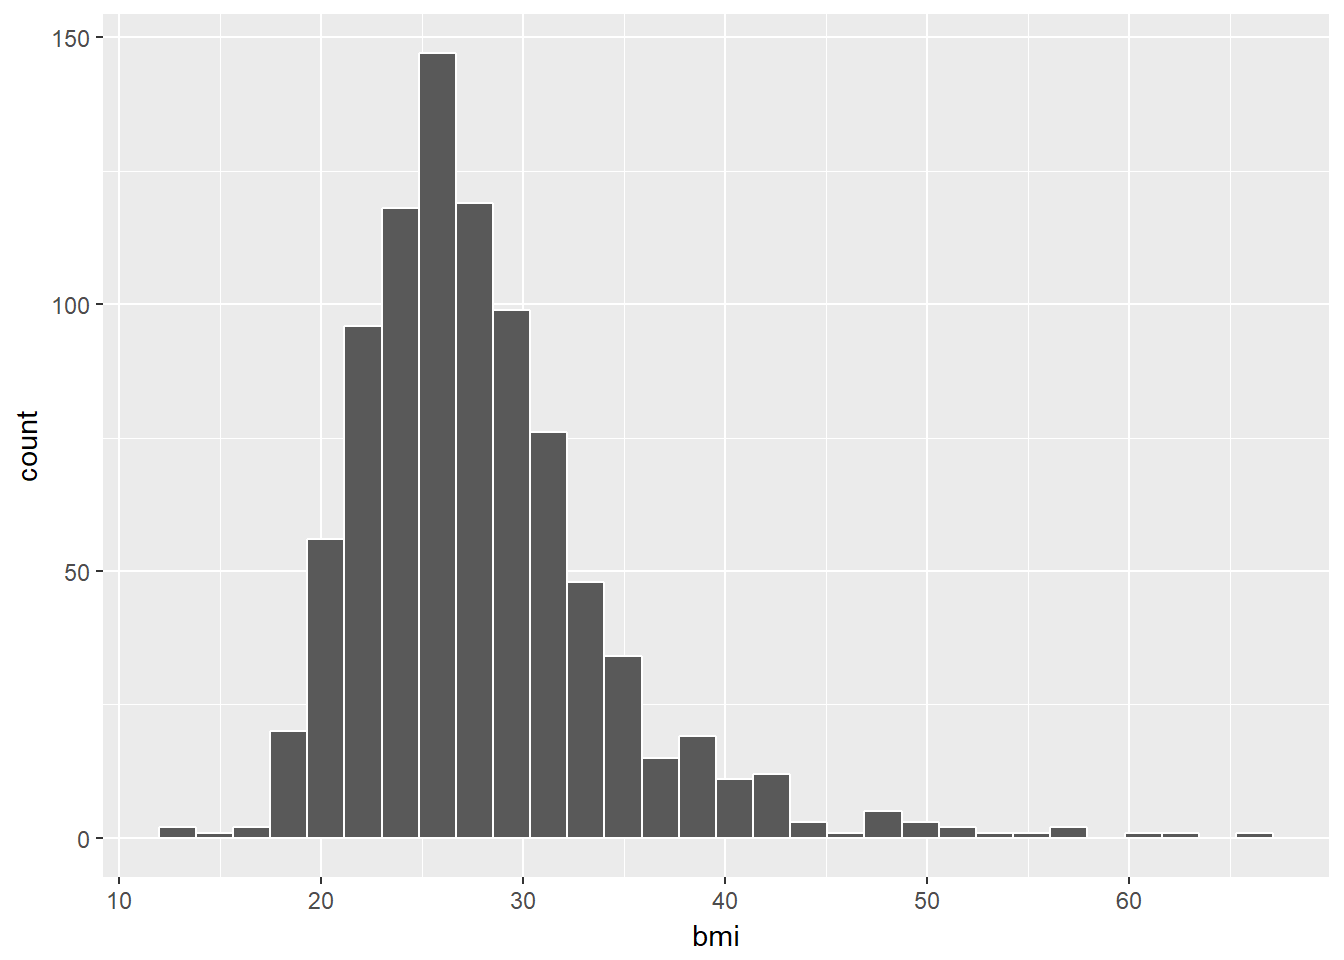
\includegraphics{bookdown-demo_files/figure-latex/c2_histogram_bmi_smartcle2-1.pdf}

\subsection{How many of the respondents have a BMI below
30?}\label{how-many-of-the-respondents-have-a-bmi-below-30}

\begin{Shaded}
\begin{Highlighting}[]
\NormalTok{smartcle2 }\OperatorTok\StringTok{ }\KeywordTok{count}\NormalTok{(bmi }\OperatorTok{<}\StringTok{ }\DecValTok{30}\NormalTok{) }\OperatorTok\StringTok{ }\KeywordTok{mutate}\NormalTok{(}\DataTypeTok{proportion =}\NormalTok{ n }\OperatorTok{/}\StringTok{ }\KeywordTok{sum}\NormalTok{(n))}
\end{Highlighting}
\end{Shaded}

\begin{verbatim}
# A tibble: 2 x 3
  `bmi < 30`     n proportion
  <lgl>      <int>      <dbl>
1 FALSE        253      0.282
2 TRUE         643      0.718
\end{verbatim}

\subsection{How many of the respondents who have a BMI \textless{} 30
exercised?}\label{how-many-of-the-respondents-who-have-a-bmi-30-exercised}

\begin{Shaded}
\begin{Highlighting}[]
\NormalTok{smartcle2 }\OperatorTok\StringTok{ }\KeywordTok{count}\NormalTok{(exerany, bmi }\OperatorTok{<}\StringTok{ }\DecValTok{30}\NormalTok{) }\OperatorTok
\StringTok{    }\KeywordTok{group_by}\NormalTok{(exerany) }\OperatorTok
\StringTok{    }\KeywordTok{mutate}\NormalTok{(}\DataTypeTok{percent =} \DecValTok{100}\OperatorTok{*}\NormalTok{n}\OperatorTok{/}\KeywordTok{sum}\NormalTok{(n))}
\end{Highlighting}
\end{Shaded}

\begin{verbatim}
# A tibble: 4 x 4
# Groups:   exerany [2]
  exerany `bmi < 30`     n percent
    <int> <lgl>      <int>   <dbl>
1       0 FALSE         88    42.1
2       0 TRUE         121    57.9
3       1 FALSE        165    24.0
4       1 TRUE         522    76.0
\end{verbatim}

\subsection{Is obesity associated with sex, in these
data?}\label{is-obesity-associated-with-sex-in-these-data}

\begin{Shaded}
\begin{Highlighting}[]
\NormalTok{smartcle2 }\OperatorTok\StringTok{ }\KeywordTok{count}\NormalTok{(female, bmi }\OperatorTok{<}\StringTok{ }\DecValTok{30}\NormalTok{) }\OperatorTok
\StringTok{    }\KeywordTok{group_by}\NormalTok{(female) }\OperatorTok
\StringTok{    }\KeywordTok{mutate}\NormalTok{(}\DataTypeTok{percent =} \DecValTok{100}\OperatorTok{*}\NormalTok{n}\OperatorTok{/}\KeywordTok{sum}\NormalTok{(n))}
\end{Highlighting}
\end{Shaded}

\begin{verbatim}
# A tibble: 4 x 4
# Groups:   female [2]
  female `bmi < 30`     n percent
   <int> <lgl>      <int>   <dbl>
1      0 FALSE        105    28.2
2      0 TRUE         267    71.8
3      1 FALSE        148    28.2
4      1 TRUE         376    71.8
\end{verbatim}

\subsection{\texorpdfstring{Comparing \texttt{sleephrs} summaries by
obesity
status}{Comparing sleephrs summaries by obesity status}}\label{comparing-sleephrs-summaries-by-obesity-status}

Can we compare the \texttt{sleephrs} means, medians and
75\textsuperscript{th} percentiles for respondents whose BMI is below 30
to the respondents whose BMI is not?

\begin{Shaded}
\begin{Highlighting}[]
\NormalTok{smartcle2 }\OperatorTok
\StringTok{    }\KeywordTok{group_by}\NormalTok{(bmi }\OperatorTok{<}\StringTok{ }\DecValTok{30}\NormalTok{) }\OperatorTok
\StringTok{    }\KeywordTok{summarize}\NormalTok{(}\KeywordTok{mean}\NormalTok{(sleephrs), }\KeywordTok{median}\NormalTok{(sleephrs), }
              \DataTypeTok{q75 =} \KeywordTok{quantile}\NormalTok{(sleephrs, }\FloatTok{0.75}\NormalTok{))}
\end{Highlighting}
\end{Shaded}

\begin{verbatim}
# A tibble: 2 x 4
  `bmi < 30` `mean(sleephrs)` `median(sleephrs)`   q75
  <lgl>                 <dbl>              <int> <dbl>
1 FALSE                  6.93                  7    8.
2 TRUE                   7.06                  7    8.
\end{verbatim}

\subsection{\texorpdfstring{The \texttt{skim} function within a
pipe}{The skim function within a pipe}}\label{the-skim-function-within-a-pipe}

The \textbf{skim} function works within pipes and with the other
\texttt{tidyverse} functions.

\begin{Shaded}
\begin{Highlighting}[]
\NormalTok{smartcle2 }\OperatorTok
\StringTok{    }\KeywordTok{group_by}\NormalTok{(exerany) }\OperatorTok
\StringTok{    }\KeywordTok{skim}\NormalTok{(bmi, sleephrs)}
\end{Highlighting}
\end{Shaded}

\begin{verbatim}
Skim summary statistics
 n obs: 896 
 n variables: 10 
 group variables: exerany 

Variable type: integer 
 exerany variable missing complete   n mean   sd p0 p25 median p75 p100
       0 sleephrs       0      209 209 7    1.85  1   6      7   8   20
       1 sleephrs       0      687 687 7.03 1.34  1   6      7   8   16

Variable type: numeric 
 exerany variable missing complete   n  mean   sd    p0   p25 median   p75
       0      bmi       0      209 209 29.57 7.46 18    24.11  28.49 33.13
       1      bmi       0      687 687 27.35 5.84 12.71 23.7   26.52 29.81
  p100
 66.06
 60.95
\end{verbatim}

\section{\texorpdfstring{First Modeling Attempt: Can \texttt{bmi}
predict
\texttt{physhealth}?}{First Modeling Attempt: Can bmi predict physhealth?}}\label{first-modeling-attempt-can-bmi-predict-physhealth}

We'll start with an effort to predict \texttt{physhealth} using
\texttt{bmi}. A natural graph would be a scatterplot.

\begin{Shaded}
\begin{Highlighting}[]
\KeywordTok{ggplot}\NormalTok{(}\DataTypeTok{data =}\NormalTok{ smartcle2, }\KeywordTok{aes}\NormalTok{(}\DataTypeTok{x =}\NormalTok{ bmi, }\DataTypeTok{y =}\NormalTok{ physhealth)) }\OperatorTok{+}
\StringTok{    }\KeywordTok{geom_point}\NormalTok{()}
\end{Highlighting}
\end{Shaded}

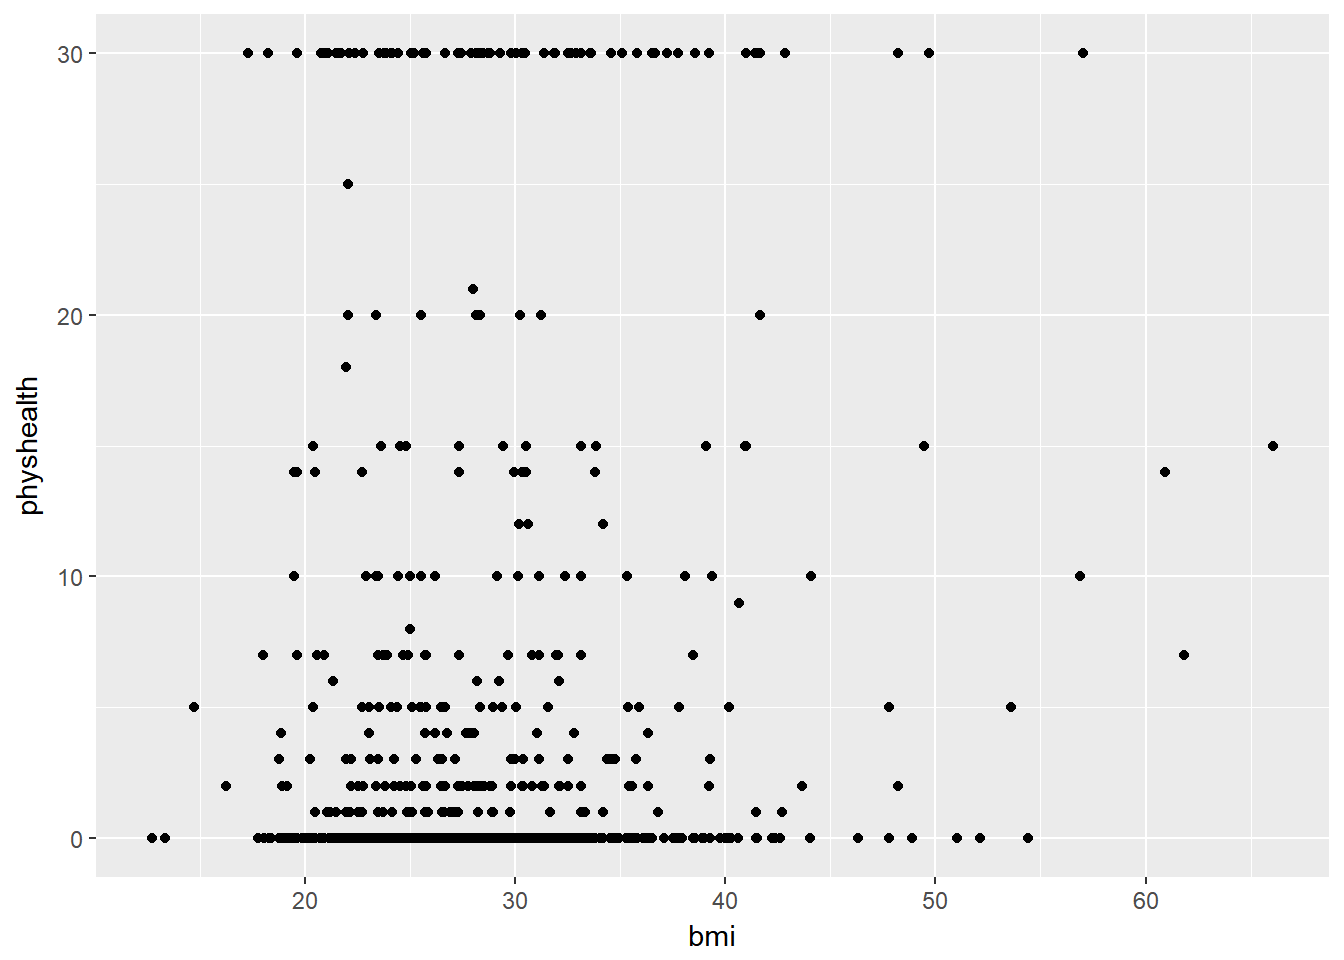
\includegraphics{bookdown-demo_files/figure-latex/scatter_physhealth_bmi_1-1.pdf}

A good question to ask ourselves here might be: ``In what BMI range can
we make a reasonable prediction of \texttt{physhealth}?''

Now, we might take the plot above and add a simple linear model \ldots{}

\begin{Shaded}
\begin{Highlighting}[]
\KeywordTok{ggplot}\NormalTok{(}\DataTypeTok{data =}\NormalTok{ smartcle2, }\KeywordTok{aes}\NormalTok{(}\DataTypeTok{x =}\NormalTok{ bmi, }\DataTypeTok{y =}\NormalTok{ physhealth)) }\OperatorTok{+}
\StringTok{    }\KeywordTok{geom_point}\NormalTok{() }\OperatorTok{+}
\StringTok{    }\KeywordTok{geom_smooth}\NormalTok{(}\DataTypeTok{method =} \StringTok{"lm"}\NormalTok{, }\DataTypeTok{se =} \OtherTok{FALSE}\NormalTok{)}
\end{Highlighting}
\end{Shaded}

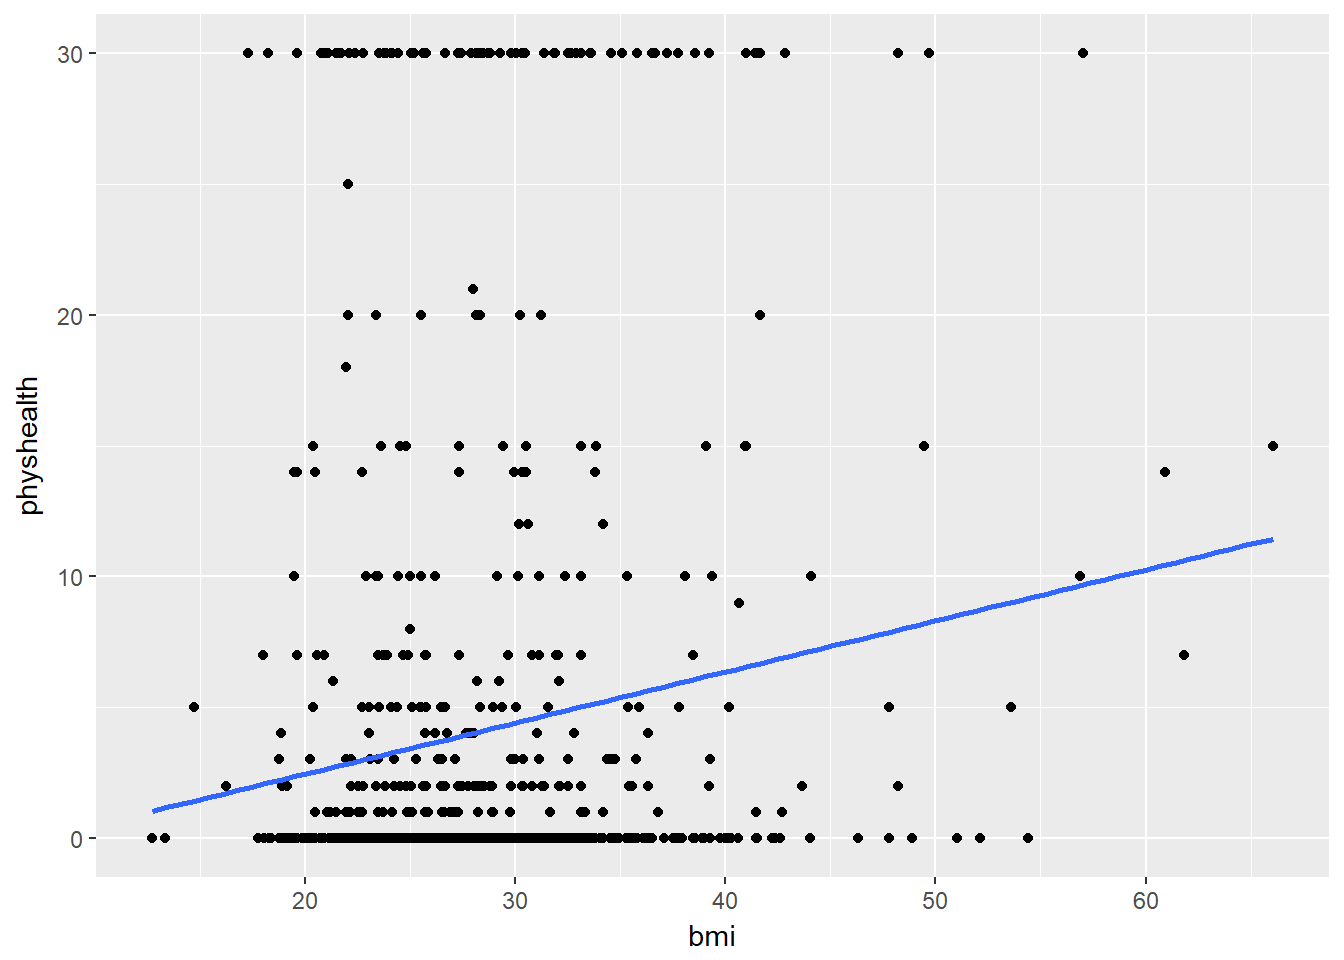
\includegraphics{bookdown-demo_files/figure-latex/c2_scatter_physhealth_bmi_2-1.pdf}

which shows the same least squares regression model that we can fit with
the \texttt{lm} command.

\subsection{Fitting a Simple Regression
Model}\label{fitting-a-simple-regression-model}

\begin{Shaded}
\begin{Highlighting}[]
\NormalTok{model_A <-}\StringTok{ }\KeywordTok{lm}\NormalTok{(physhealth }\OperatorTok{~}\StringTok{ }\NormalTok{bmi, }\DataTypeTok{data =}\NormalTok{ smartcle2)}

\NormalTok{model_A}
\end{Highlighting}
\end{Shaded}

\begin{verbatim}

Call:
lm(formula = physhealth ~ bmi, data = smartcle2)

Coefficients:
(Intercept)          bmi  
    -1.4514       0.1953  
\end{verbatim}

\begin{Shaded}
\begin{Highlighting}[]
\KeywordTok{summary}\NormalTok{(model_A)}
\end{Highlighting}
\end{Shaded}

\begin{verbatim}

Call:
lm(formula = physhealth ~ bmi, data = smartcle2)

Residuals:
   Min     1Q Median     3Q    Max 
-9.171 -4.057 -3.193 -1.576 28.073 

Coefficients:
            Estimate Std. Error t value Pr(>|t|)    
(Intercept) -1.45143    1.29185  -1.124    0.262    
bmi          0.19527    0.04521   4.319 1.74e-05 ***
---
Signif. codes:  0 '***' 0.001 '**' 0.01 '*' 0.05 '.' 0.1 ' ' 1

Residual standard error: 8.556 on 894 degrees of freedom
Multiple R-squared:  0.02044,   Adjusted R-squared:  0.01934 
F-statistic: 18.65 on 1 and 894 DF,  p-value: 1.742e-05
\end{verbatim}

\begin{Shaded}
\begin{Highlighting}[]
\KeywordTok{confint}\NormalTok{(model_A, }\DataTypeTok{level =} \FloatTok{0.95}\NormalTok{)}
\end{Highlighting}
\end{Shaded}

\begin{verbatim}
                 2.5 %    97.5 %
(Intercept) -3.9868457 1.0839862
bmi          0.1065409 0.2840068
\end{verbatim}

The model coefficients can be obtained by printing the model object, and
the \texttt{summary} function provides several useful descriptions of
the model's residuals, its statistical significance, and quality of fit.

\subsection{Model Summary for a Simple (One-Predictor)
Regression}\label{model-summary-for-a-simple-one-predictor-regression}

The fitted model predicts \texttt{physhealth} with the equation -1.45 +
0.195*\texttt{bmi}, as we can read off from the model coefficients.

Each of the 896 respondents included in the \texttt{smartcle2} data
makes a contribution to this model.

\subsubsection{Residuals}\label{residuals}

Suppose Harry is one of the people in that group, and Harry's data is
\texttt{bmi} = 20, and \texttt{physhealth} = 3.

\begin{itemize}
\tightlist
\item
  Harry's \emph{observed} value of \texttt{physhealth} is just the value
  we have in the data for them, in this case, observed
  \texttt{physhealth} = 3 for Harry.
\item
  Harry's \emph{fitted} or \emph{predicted} \texttt{physhealth} value is
  the result of calculating -1.45 + 0.195*\texttt{bmi} for Harry. So, if
  Harry's BMI was 20, then Harry's predicted \texttt{physhealth} value
  is -1.45 + (0.195)(20) = 2.45.
\item
  The \emph{residual} for Harry is then his \emph{observed} outcome
  minus his \emph{fitted} outcome, so Harry has a residual of 3 - 2.45 =
  0.55.
\item
  Graphically, a residual represents vertical distance between the
  observed point and the fitted regression line.
\item
  Points above the regression line will have positive residuals, and
  points below the regression line will have negative residuals. Points
  on the line have zero residuals.
\end{itemize}

The residuals are summarized at the top of the \texttt{summary} output
for linear model.

\begin{itemize}
\tightlist
\item
  The mean residual will always be zero in an ordinary least squares
  model, but a five number summary of the residuals is provided by the
  summary, as is an estimated standard deviation of the residuals
  (called here the Residual standard error.)
\item
  In the \texttt{smartcle2} data, the minimum residual was -9.17, so for
  one subject, the observed value was 9.17 days smaller than the
  predicted value. This means that the prediction was 9.17 days too
  large for that subject.
\item
  Similarly, the maximum residual was 28.07 days, so for one subject the
  prediction was 28.07 days too small. Not a strong performance.
\item
  In a least squares model, the residuals are assumed to follow a Normal
  distribution, with mean zero, and standard deviation (for the
  \texttt{smartcle2} data) of about 8.6 days. Thus, by the definition of
  a Normal distribution, we'd expect
\item
  about 68\% of the residuals to be between -8.6 and +8.6 days,
\item
  about 95\% of the residuals to be between -17.2 and +17.2 days,
\item
  about all (99.7\%) of the residuals to be between -25.8 and +25.8
  days.
\end{itemize}

\subsubsection{Coefficients section}\label{coefficients-section}

The \texttt{summary} for a linear model shows Estimates, Standard
Errors, t values and \emph{p} values for each coefficient fit.

\begin{itemize}
\tightlist
\item
  The Estimates are the point estimates of the intercept and slope of
  \texttt{bmi} in our model.
\item
  In this case, our estimated slope is 0.195, which implies that if
  Harry's BMI is 20 and Sally's BMI is 21, we predict that Sally's
  \texttt{physhealth} will be 0.195 days larger than Harry's.
\item
  The Standard Errors are also provided for each estimate. We can create
  rough 95\% confidence intervals by adding and subtracting two standard
  errors from each coefficient, or we can get a slightly more accurate
  answer with the \texttt{confint} function.
\item
  Here, the 95\% confidence interval for the slope of \texttt{bmi} is
  estimated to be (0.11, 0.28). This is a good measure of the
  uncertainty in the slope that is captured by our model. We are 95\%
  confident in the process of building this interval, but this doesn't
  mean we're 95\% sure that the true slope is actually in that interval.
\end{itemize}

Also available are a \emph{t} value (just the Estimate divided by the
Standard Error) and the appropriate \emph{p} value for testing the null
hypothesis that the true value of the coefficient is 0 against a
two-tailed alternative.

\begin{itemize}
\tightlist
\item
  If a slope coefficient is statistically significantly different from
  0, this implies that 0 will not be part of the uncertainty interval
  obtained through \texttt{confint}.
\item
  If the slope was zero, it would suggest that \texttt{bmi} would add no
  predictive value to the model. But that's unlikely here.
\end{itemize}

If the \texttt{bmi} slope coefficient is associated with a small
\emph{p} value, as in the case of our \texttt{model\_A}, it suggests
that the model including \texttt{bmi} is statistically significantly
better at predicting \texttt{physhealth} than the model without
\texttt{bmi}.

\begin{itemize}
\tightlist
\item
  Without \texttt{bmi} our \texttt{model\_A} would become an
  \emph{intercept-only} model, in this case, which would predict the
  mean \texttt{physhealth} for everyone, regardless of any other
  information.
\end{itemize}

\subsubsection{Model Fit Summaries}\label{model-fit-summaries}

The \texttt{summary} of a linear model also displays:

\begin{itemize}
\tightlist
\item
  The residual standard error and associated degrees of freedom for the
  residuals.
\item
  For a simple (one-predictor) least regression like this, the residual
  degrees of freedom will be the sample size minus 2.
\item
  The multiple R-squared (or coefficient of determination)
\item
  This is interpreted as the proportion of variation in the outcome
  (\texttt{physhealth}) accounted for by the model, and will always fall
  between 0 and 1 as a result.
\item
  Our model\_A accounts for a mere 2\% of the variation in
  \texttt{physhealth}.
\item
  The Adjusted R-squared value ``adjusts'' for the size of our model in
  terms of the number of coefficients included in the model.
\item
  The adjusted R-squared will always be less than the Multiple
  R-squared.
\item
  We still hope to find models with relatively large adjusted
  R\textsuperscript{2} values.
\item
  In particular, we hope to find models where the adjusted
  R\textsuperscript{2} isn't substantially less than the Multiple
  R-squared.
\item
  The adjusted R-squared is usually a better estimate of likely
  performance of our model in new data than is the Multiple R-squared.
\item
  The adjusted R-squared result is no longer interpretable as a
  proportion of anything - in fact, it can fall below 0.
\item
  We can obtain the adjusted R\textsuperscript{2} from the raw
  R\textsuperscript{2}, the number of observations \emph{N} and the
  number of predictors \emph{p} included in the model, as follows:
\end{itemize}

\[
R^2_{adj} = 1 - \frac{(1 - R^2)(N - 1)}{N - p - 1},
\]

\begin{itemize}
\tightlist
\item
  The F statistic and \emph{p} value from a global ANOVA test of the
  model.

  \begin{itemize}
  \tightlist
  \item
    Obtaining a statistically significant result here is usually pretty
    straightforward, since the comparison is between our model, and a
    model which simply predicts the mean value of the outcome for
    everyone.
  \item
    In a simple (one-predictor) linear regression like this, the t
    statistic for the slope is just the square root of the F statistic,
    and the resulting \emph{p} values for the slope's t test and for the
    global F test will be identical.
  \end{itemize}
\item
  To see the complete ANOVA F test for this model, we can run
  \texttt{anova(model\_A)}.
\end{itemize}

\begin{Shaded}
\begin{Highlighting}[]
\KeywordTok{anova}\NormalTok{(model_A)}
\end{Highlighting}
\end{Shaded}

\begin{verbatim}
Analysis of Variance Table

Response: physhealth
           Df Sum Sq Mean Sq F value    Pr(>F)    
bmi         1   1366  1365.5  18.655 1.742e-05 ***
Residuals 894  65441    73.2                      
---
Signif. codes:  0 '***' 0.001 '**' 0.01 '*' 0.05 '.' 0.1 ' ' 1
\end{verbatim}

\subsection{\texorpdfstring{Using the \texttt{broom}
package}{Using the broom package}}\label{using-the-broom-package}

The \texttt{broom} package has three functions of particular use in a
linear regression model:

\subsubsection{\texorpdfstring{The \texttt{tidy}
function}{The tidy function}}\label{the-tidy-function}

\texttt{tidy} builds a data frame/tibble containing information about
the coefficients in the model, their standard errors, t statistics and
\emph{p} values.

\begin{Shaded}
\begin{Highlighting}[]
\KeywordTok{tidy}\NormalTok{(model_A)}
\end{Highlighting}
\end{Shaded}

\begin{verbatim}
         term   estimate  std.error statistic      p.value
1 (Intercept) -1.4514298 1.29185199 -1.123526 2.615156e-01
2         bmi  0.1952739 0.04521145  4.319125 1.741859e-05
\end{verbatim}

\subsubsection{\texorpdfstring{The \texttt{glance}
function}{The glance function}}\label{the-glance-function}

glance` builds a data frame/tibble containing summary statistics about
the model, including

\begin{itemize}
\tightlist
\item
  the (raw) multiple R\textsuperscript{2} and adjusted R\^{}2
\item
  \texttt{sigma} which is the residual standard error
\item
  the F \texttt{statistic}, \texttt{p.value} model \texttt{df} and
  \texttt{df.residual} associated with the global ANOVA test, plus
\item
  several statistics that will be useful in comparing models down the
  line:
\item
  the model's log likelihood function value, \texttt{logLik}
\item
  the model's Akaike's Information Criterion value, \texttt{AIC}
\item
  the model's Bayesian Information Criterion value, \texttt{BIC}
\item
  and the model's \texttt{deviance} statistic
\end{itemize}

\begin{Shaded}
\begin{Highlighting}[]
\KeywordTok{glance}\NormalTok{(model_A)}
\end{Highlighting}
\end{Shaded}

\begin{verbatim}
   r.squared adj.r.squared    sigma statistic      p.value df    logLik
1 0.02044019    0.01934449 8.555737  18.65484 1.741859e-05  2 -3193.723
       AIC     BIC deviance df.residual
1 6393.446 6407.84 65441.36         894
\end{verbatim}

\subsubsection{\texorpdfstring{The \texttt{augment}
function}{The augment function}}\label{the-augment-function}

\texttt{augment} builds a data frame/tibble which adds fitted values,
residuals and other diagnostic summaries that describe each observation
to the original data used to fit the model, and this includes

\begin{itemize}
\tightlist
\item
  \texttt{.fitted} and \texttt{.resid}, the fitted and residual values,
  in addition to
\item
  \texttt{.hat}, the leverage value for this observation
\item
  \texttt{.cooksd}, the Cook's distance measure of \emph{influence} for
  this observation
\item
  \texttt{.stdresid}, the standardized residual (think of this as a
  z-score - a measure of the residual divided by its associated standard
  deviation \texttt{.sigma})
\item
  and \texttt{se.fit} which will help us generate prediction intervals
  for the model downstream
\end{itemize}

Note that each of the new columns begins with \texttt{.} to avoid
overwriting any data.

\begin{Shaded}
\begin{Highlighting}[]
\KeywordTok{head}\NormalTok{(}\KeywordTok{augment}\NormalTok{(model_A))}
\end{Highlighting}
\end{Shaded}

\begin{verbatim}
  physhealth   bmi  .fitted   .se.fit      .resid        .hat   .sigma
1          0 26.69 3.760430 0.2907252 -3.76043009 0.001154651 8.559600
2          0 23.70 3.176561 0.3422908 -3.17656119 0.001600574 8.559865
3          1 26.92 3.805343 0.2890054 -2.80534308 0.001141030 8.560010
4          0 21.66 2.778202 0.4005101 -2.77820248 0.002191352 8.560020
5          5 24.09 3.252718 0.3329154  1.74728200 0.001514095 8.560326
6          4 27.64 3.945940 0.2860087  0.05405972 0.001117490 8.560526
       .cooksd   .std.resid
1 1.117852e-04 -0.439775451
2 1.106717e-04 -0.371575999
3 6.147744e-05 -0.328077528
4 1.160381e-04 -0.325074461
5 3.167016e-05  0.204378225
6 2.235722e-08  0.006322069
\end{verbatim}

For more on the \texttt{broom} package, you may want to look at
\href{https://cran.r-project.org/web/packages/broom/vignettes/broom.html}{this
vignette}.

\subsection{How does the model do? (Residuals vs.~Fitted
Values)}\label{how-does-the-model-do-residuals-vs.fitted-values}

\begin{itemize}
\tightlist
\item
  Remember that the R\textsuperscript{2} value was about 2\%.
\end{itemize}

\begin{Shaded}
\begin{Highlighting}[]
\KeywordTok{plot}\NormalTok{(model_A, }\DataTypeTok{which =} \DecValTok{1}\NormalTok{)}
\end{Highlighting}
\end{Shaded}

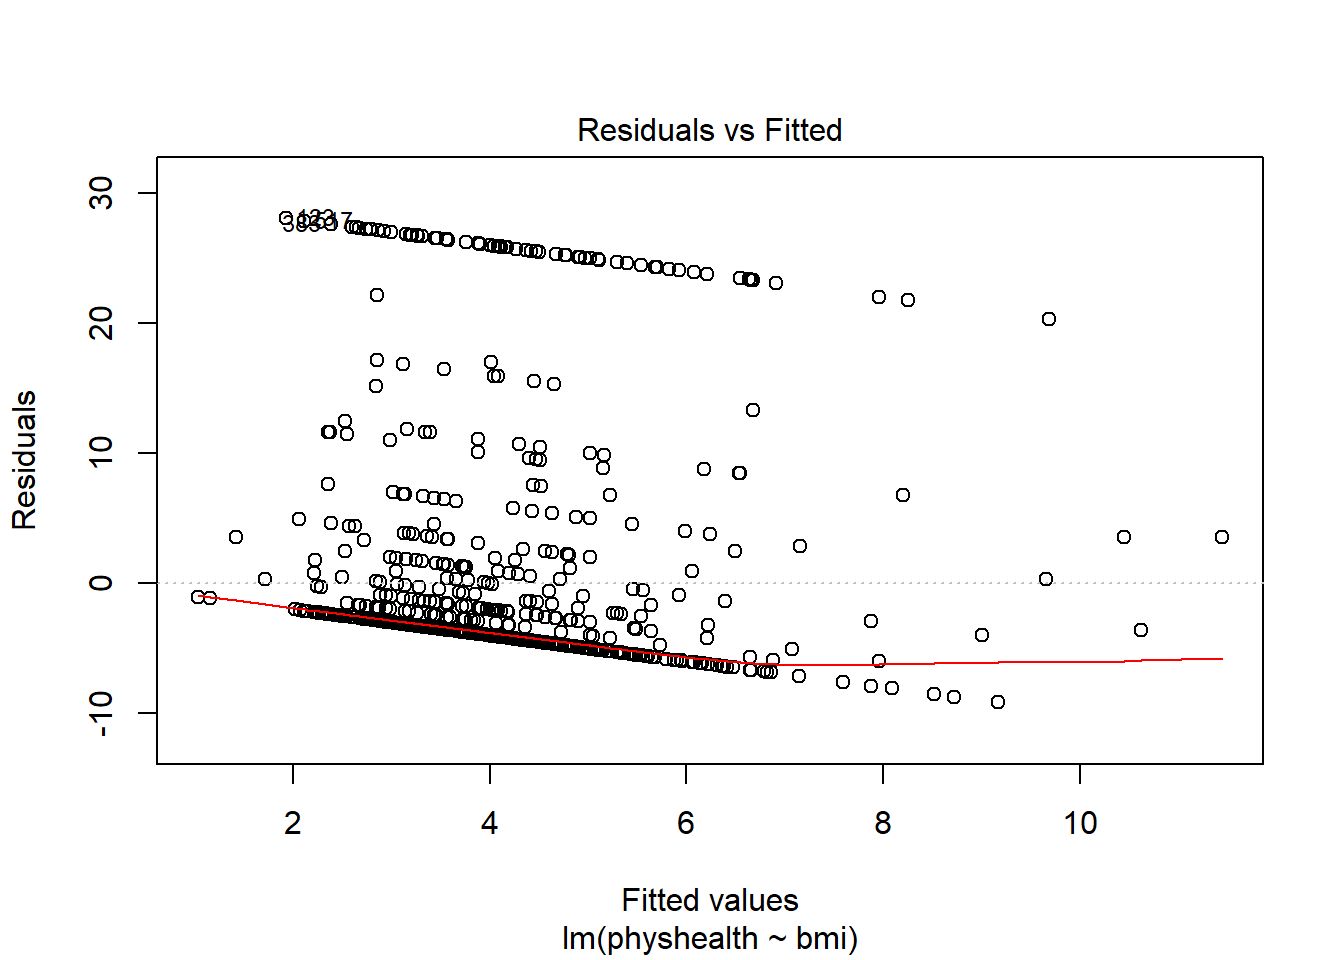
\includegraphics{bookdown-demo_files/figure-latex/chapter2_first_resid_plot_model_A-1.pdf}

This is a plot of residuals vs.~fitted values. The goal here is for this
plot to look like a random scatter of points, perhaps like a ``fuzzy
football'', and that's \textbf{not} what we have. Why?

If you prefer, here's a \texttt{ggplot2} version of a similar plot, now
looking at standardized residuals instead of raw residuals, and adding a
loess smooth and a linear fit to the result.

\begin{Shaded}
\begin{Highlighting}[]
\KeywordTok{ggplot}\NormalTok{(}\KeywordTok{augment}\NormalTok{(model_A), }\KeywordTok{aes}\NormalTok{(}\DataTypeTok{x =}\NormalTok{ .fitted, }\DataTypeTok{y =}\NormalTok{ .std.resid)) }\OperatorTok{+}
\StringTok{    }\KeywordTok{geom_point}\NormalTok{() }\OperatorTok{+}
\StringTok{    }\KeywordTok{geom_smooth}\NormalTok{(}\DataTypeTok{method =} \StringTok{"lm"}\NormalTok{, }\DataTypeTok{se =} \OtherTok{FALSE}\NormalTok{, }\DataTypeTok{col =} \StringTok{"red"}\NormalTok{, }\DataTypeTok{linetype =} \StringTok{"dashed"}\NormalTok{) }\OperatorTok{+}
\StringTok{    }\KeywordTok{geom_smooth}\NormalTok{(}\DataTypeTok{method =} \StringTok{"loess"}\NormalTok{, }\DataTypeTok{se =} \OtherTok{FALSE}\NormalTok{, }\DataTypeTok{col =} \StringTok{"navy"}\NormalTok{) }\OperatorTok{+}
\StringTok{    }\KeywordTok{theme_bw}\NormalTok{()}
\end{Highlighting}
\end{Shaded}

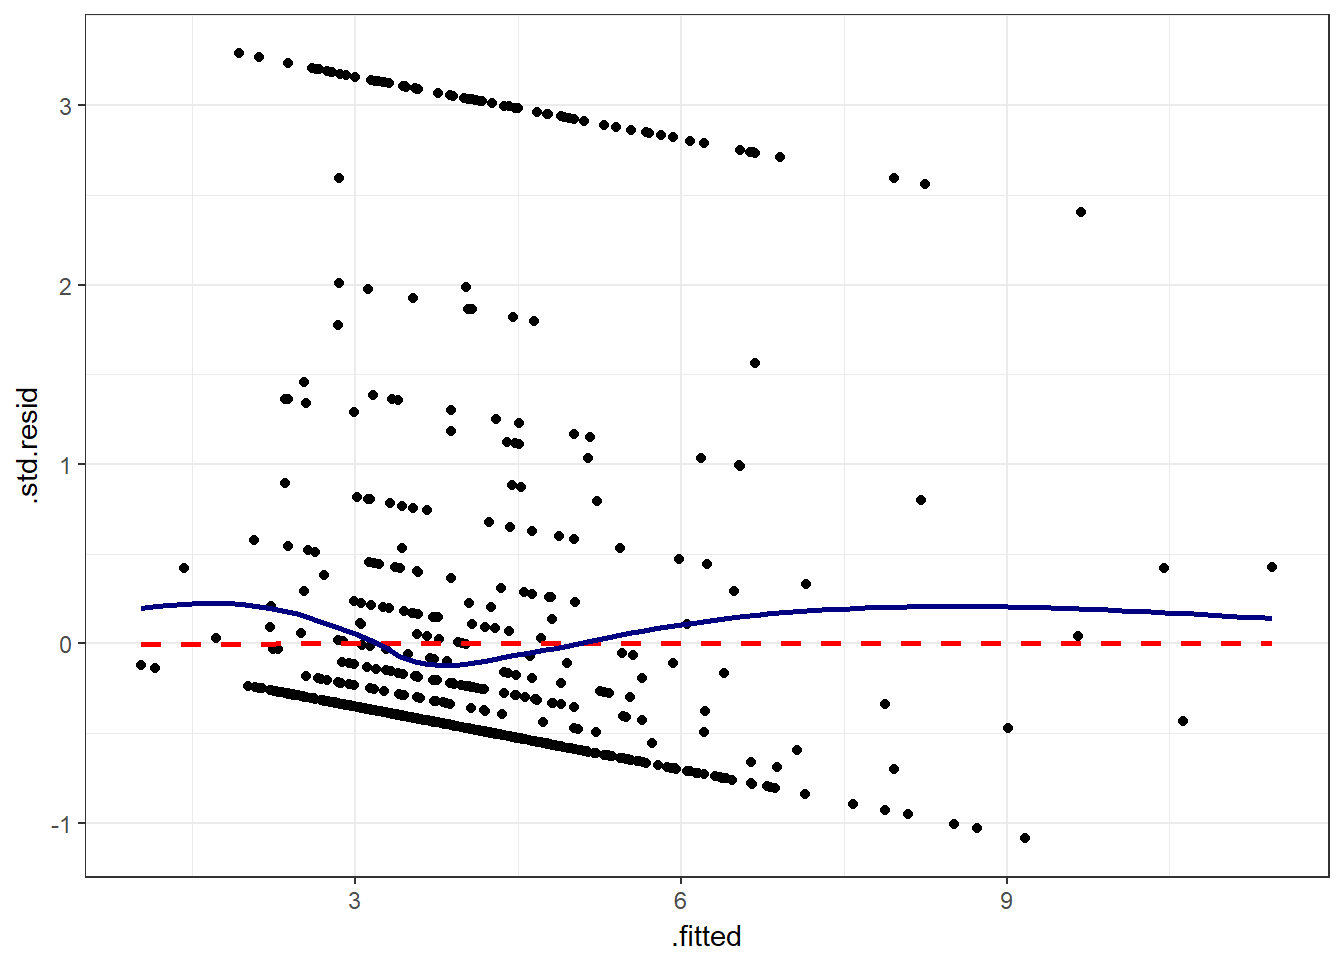
\includegraphics{bookdown-demo_files/figure-latex/chapter2_ggplot_first_resid_plot_model_A-1.pdf}

The problem we're having here becomes, I think, a little more obvious if
we look at what we're predicting. Does \texttt{physhealth} look like a
good candidate for a linear model?

\begin{Shaded}
\begin{Highlighting}[]
\KeywordTok{ggplot}\NormalTok{(smartcle2, }\KeywordTok{aes}\NormalTok{(}\DataTypeTok{x =}\NormalTok{ physhealth)) }\OperatorTok{+}
\KeywordTok{geom_histogram}\NormalTok{(}\DataTypeTok{bins =} \DecValTok{30}\NormalTok{, }\DataTypeTok{fill =} \StringTok{"dodgerblue"}\NormalTok{, }\DataTypeTok{color =} \StringTok{"royalblue"}\NormalTok{)}
\end{Highlighting}
\end{Shaded}

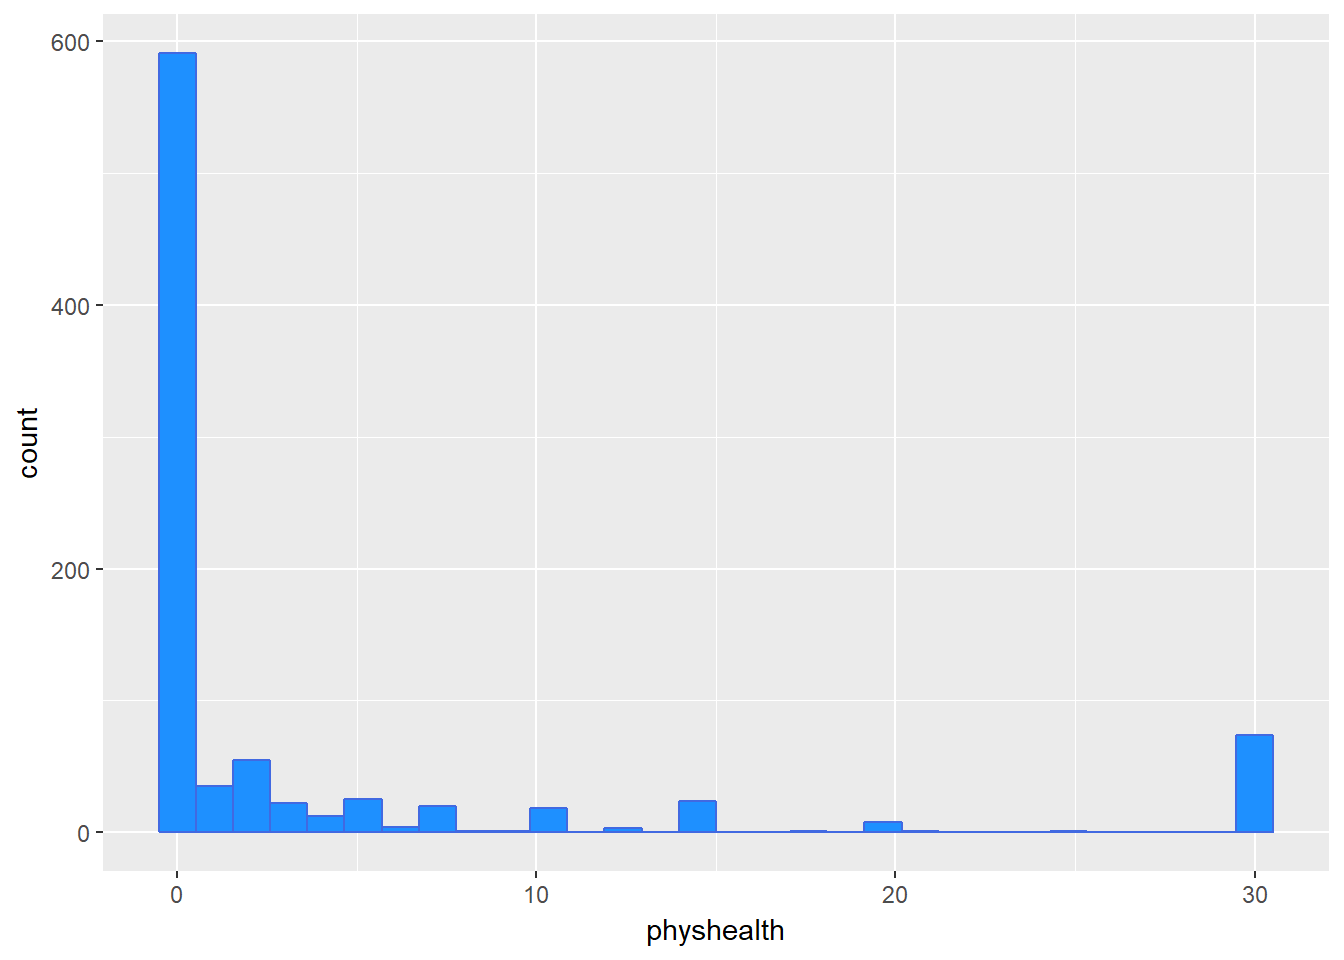
\includegraphics{bookdown-demo_files/figure-latex/histogram_of_physhealth_smartcle2-1.pdf}

\begin{Shaded}
\begin{Highlighting}[]
\NormalTok{smartcle2 }\OperatorTok\StringTok{ }\KeywordTok{count}\NormalTok{(physhealth }\OperatorTok{==}\StringTok{ }\DecValTok{0}\NormalTok{, physhealth }\OperatorTok{==}\StringTok{ }\DecValTok{30}\NormalTok{)}
\end{Highlighting}
\end{Shaded}

\begin{verbatim}
# A tibble: 3 x 3
  `physhealth == 0` `physhealth == 30`     n
  <lgl>             <lgl>              <int>
1 FALSE             FALSE                231
2 FALSE             TRUE                  74
3 TRUE              FALSE                591
\end{verbatim}

No matter what model we fit, if we are predicting \texttt{physhealth},
and most of the data are values of 0 and 30, we have limited variation
in our outcome, and so our linear model will be somewhat questionable
just on that basis.

A normal Q-Q plot of the standardized residuals for our
\texttt{model\_A} shows this problem, too.

\begin{Shaded}
\begin{Highlighting}[]
\KeywordTok{plot}\NormalTok{(model_A, }\DataTypeTok{which =} \DecValTok{2}\NormalTok{)}
\end{Highlighting}
\end{Shaded}

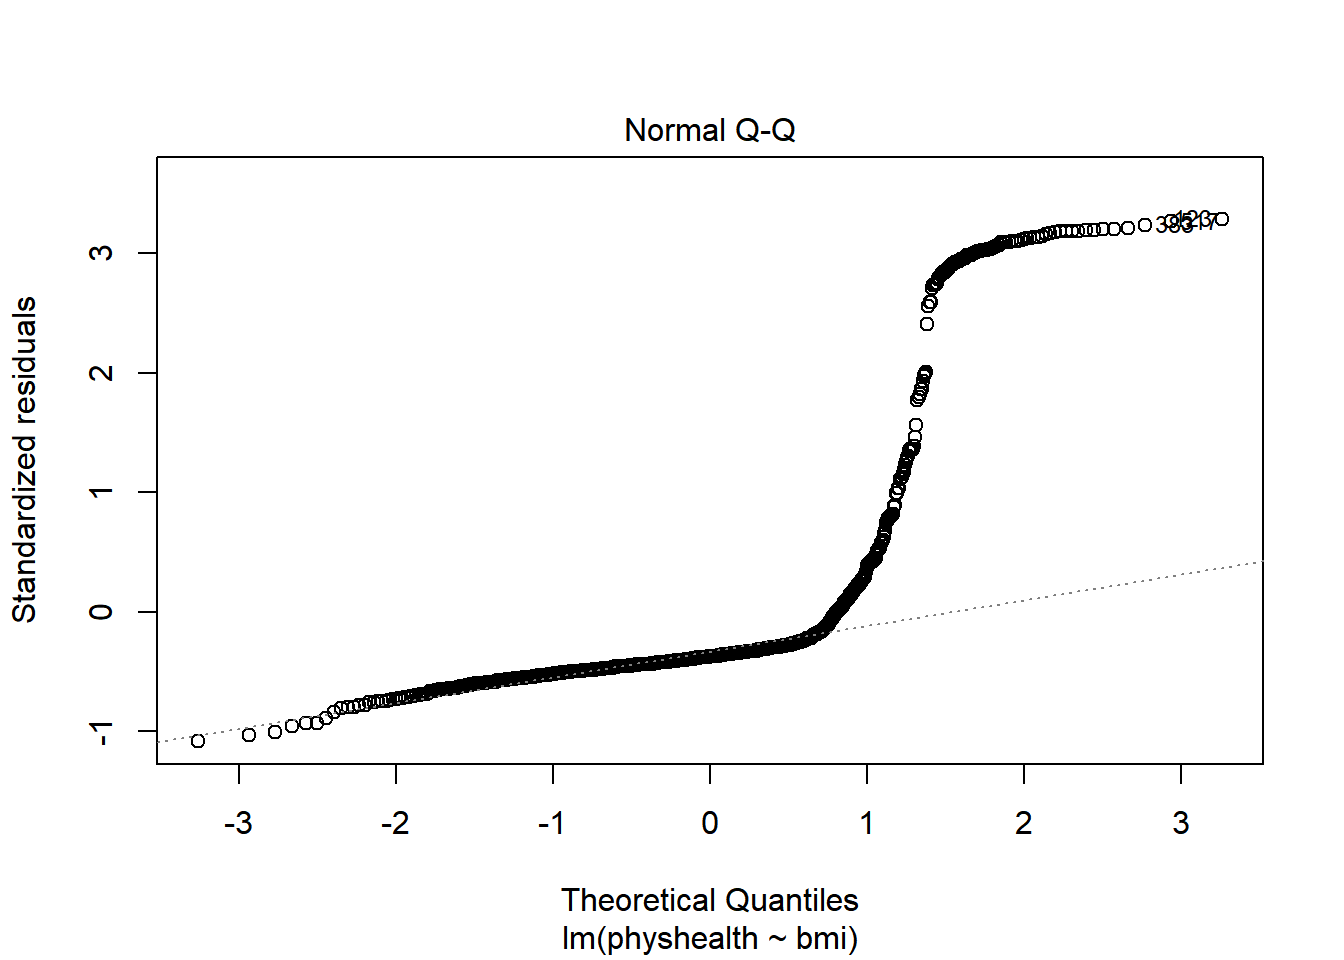
\includegraphics{bookdown-demo_files/figure-latex/chapter2_second_resid_plot_model_A-1.pdf}

We're going to need a method to deal with this sort of outcome, that has
both a floor and a ceiling. We'll get there eventually, but linear
regression alone doesn't look promising.

All right, so that didn't go anywhere great. Let's try again, with a new
outcome.

\section{A New Small Study: Predicting
BMI}\label{a-new-small-study-predicting-bmi}

We'll begin by investigating the problem of predicting \texttt{bmi}, at
first with just three regression inputs: \texttt{sex}, \texttt{exerany}
and \texttt{sleephrs}, in our new \texttt{smartcle2} data set.

\begin{itemize}
\tightlist
\item
  The outcome of interest is \texttt{bmi}.
\item
  Inputs to the regression model are:

  \begin{itemize}
  \tightlist
  \item
    \texttt{female} = 1 if the subject is female, and 0 if they are male
  \item
    \texttt{exerany} = 1 if the subject exercised in the past 30 days,
    and 0 if they didn't
  \item
    \texttt{sleephrs} = hours slept in a typical 24-hour period (treated
    as quantitative)
  \end{itemize}
\end{itemize}

\subsection{\texorpdfstring{Does \texttt{female} predict \texttt{bmi}
well?}{Does female predict bmi well?}}\label{does-female-predict-bmi-well}

\subsubsection{Graphical Assessment}\label{graphical-assessment}

\begin{Shaded}
\begin{Highlighting}[]
\KeywordTok{ggplot}\NormalTok{(smartcle2, }\KeywordTok{aes}\NormalTok{(}\DataTypeTok{x =}\NormalTok{ female, }\DataTypeTok{y =}\NormalTok{ bmi)) }\OperatorTok{+}
\StringTok{    }\KeywordTok{geom_point}\NormalTok{()}
\end{Highlighting}
\end{Shaded}

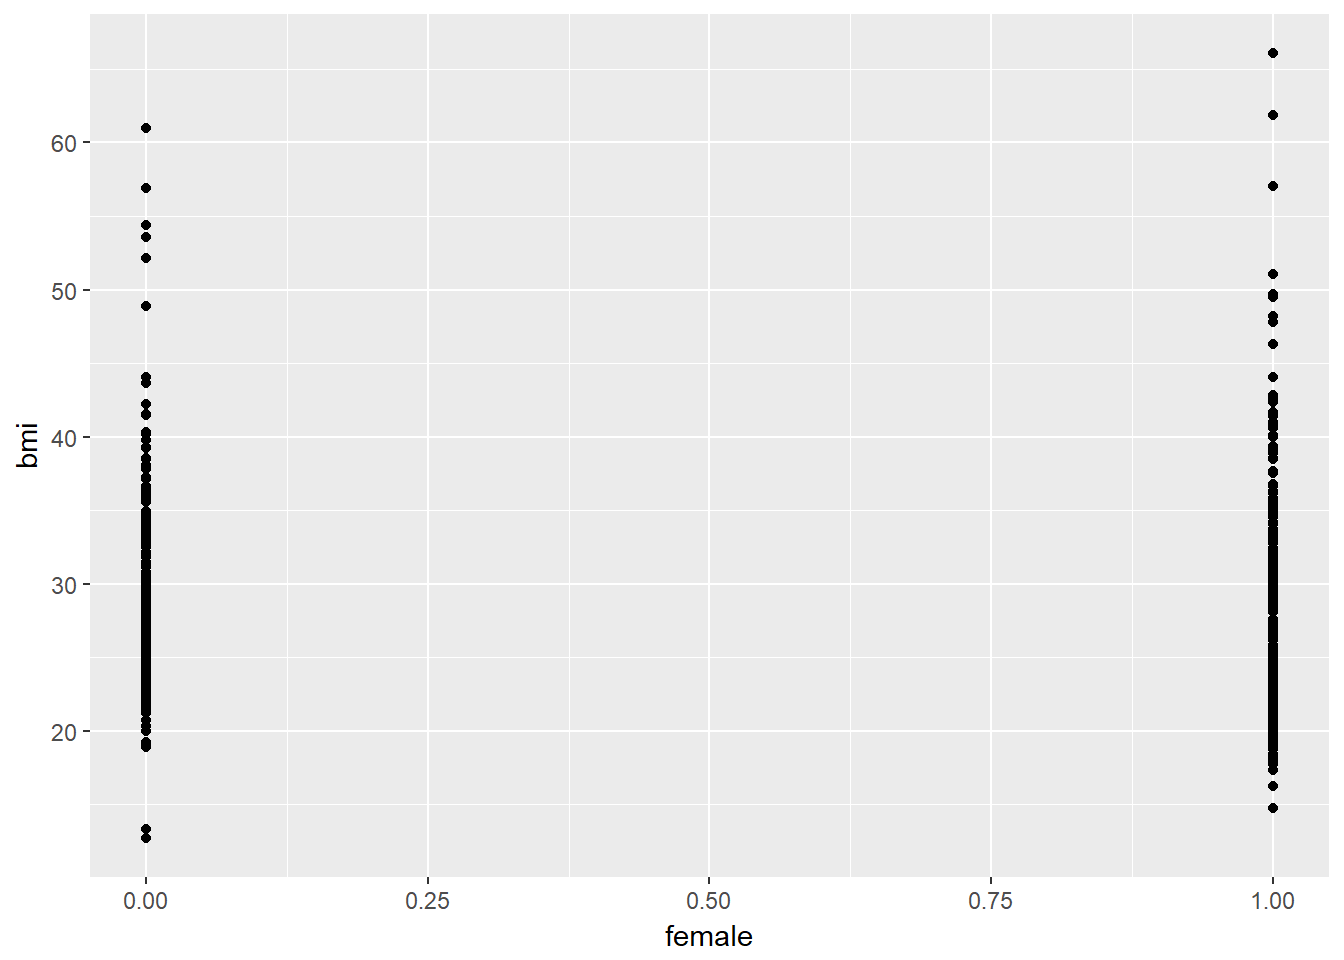
\includegraphics{bookdown-demo_files/figure-latex/c2_sex_bmi_plot1-1.pdf}

Not so helpful. We should probably specify that \texttt{female} is a
factor, and try another plotting approach.

\begin{Shaded}
\begin{Highlighting}[]
\KeywordTok{ggplot}\NormalTok{(smartcle2, }\KeywordTok{aes}\NormalTok{(}\DataTypeTok{x =} \KeywordTok{factor}\NormalTok{(female), }\DataTypeTok{y =}\NormalTok{ bmi)) }\OperatorTok{+}
\StringTok{    }\KeywordTok{geom_boxplot}\NormalTok{()}
\end{Highlighting}
\end{Shaded}

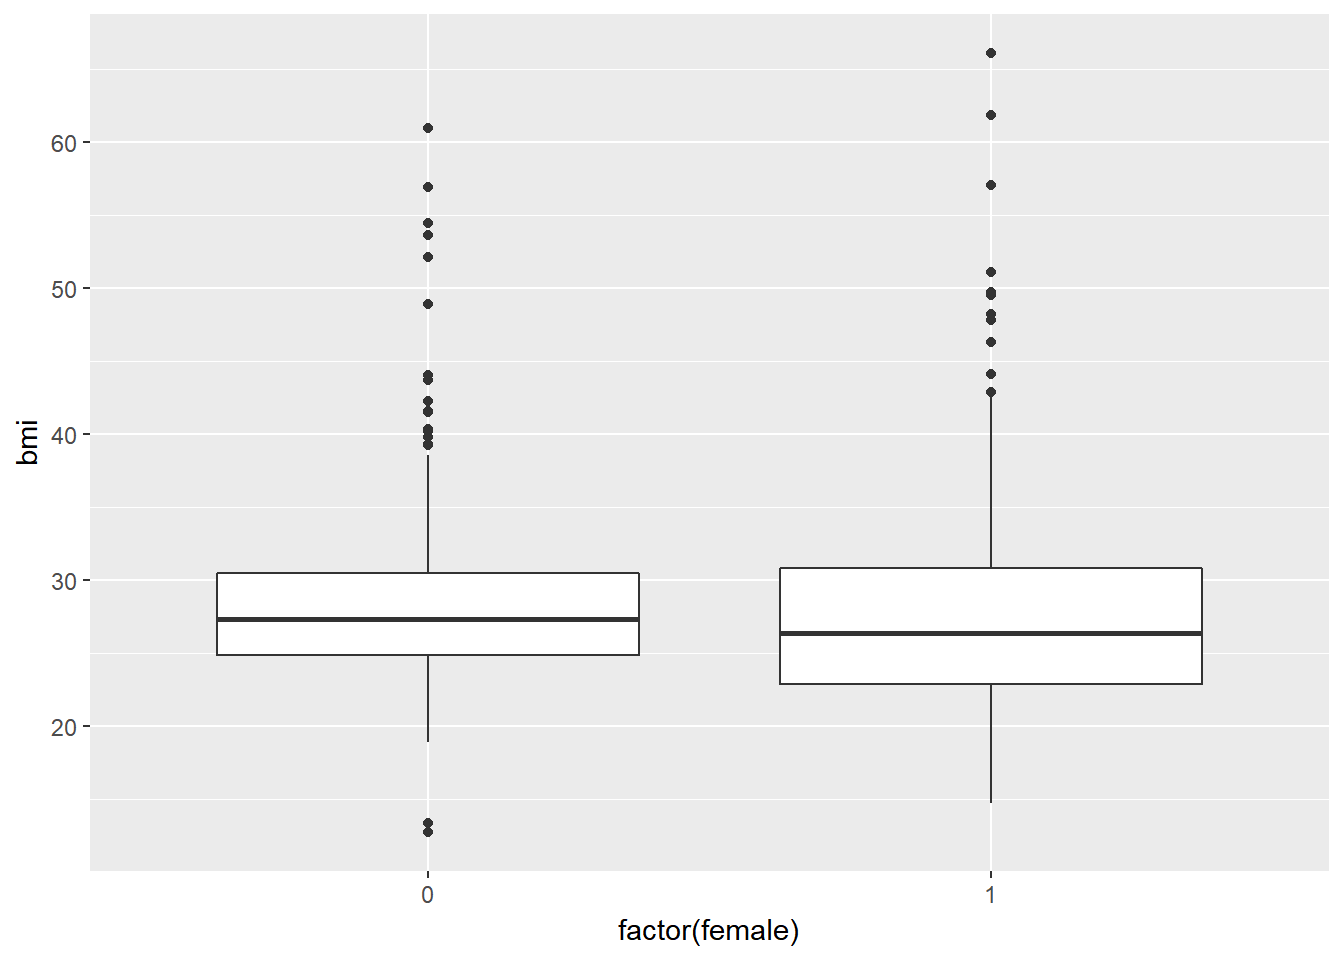
\includegraphics{bookdown-demo_files/figure-latex/c2_sex_bmi_plot2-1.pdf}

The median BMI looks a little higher for males. Let's see if a model
reflects that.

\section{\texorpdfstring{\texttt{c2\_m1}: A simple t-test
model}{c2\_m1: A simple t-test model}}\label{c2_m1-a-simple-t-test-model}

\begin{Shaded}
\begin{Highlighting}[]
\NormalTok{c2_m1 <-}\StringTok{ }\KeywordTok{lm}\NormalTok{(bmi }\OperatorTok{~}\StringTok{ }\NormalTok{female, }\DataTypeTok{data =}\NormalTok{ smartcle2)}
\NormalTok{c2_m1}
\end{Highlighting}
\end{Shaded}

\begin{verbatim}

Call:
lm(formula = bmi ~ female, data = smartcle2)

Coefficients:
(Intercept)       female  
    28.3600      -0.8457  
\end{verbatim}

\begin{Shaded}
\begin{Highlighting}[]
\KeywordTok{summary}\NormalTok{(c2_m1)}
\end{Highlighting}
\end{Shaded}

\begin{verbatim}

Call:
lm(formula = bmi ~ female, data = smartcle2)

Residuals:
    Min      1Q  Median      3Q     Max 
-15.650  -4.129  -1.080   2.727  38.546 

Coefficients:
            Estimate Std. Error t value Pr(>|t|)    
(Intercept)  28.3600     0.3274  86.613   <2e-16 ***
female       -0.8457     0.4282  -1.975   0.0485 *  
---
Signif. codes:  0 '***' 0.001 '**' 0.01 '*' 0.05 '.' 0.1 ' ' 1

Residual standard error: 6.315 on 894 degrees of freedom
Multiple R-squared:  0.004345,  Adjusted R-squared:  0.003231 
F-statistic: 3.902 on 1 and 894 DF,  p-value: 0.04855
\end{verbatim}

\begin{Shaded}
\begin{Highlighting}[]
\KeywordTok{confint}\NormalTok{(c2_m1)}
\end{Highlighting}
\end{Shaded}

\begin{verbatim}
                2.5 %      97.5 %
(Intercept) 27.717372 29.00262801
female      -1.686052 -0.00539878
\end{verbatim}

The model suggests, based on these 896 subjects, that

\begin{itemize}
\tightlist
\item
  our best prediction for males is BMI = 28.36 kg/m\textsuperscript{2},
  and
\item
  our best prediction for females is BMI = 28.36 - 0.85 = 27.51
  kg/m\textsuperscript{2}.
\item
  the mean difference between females and males is -0.85
  kg/m\textsuperscript{2} in BMI
\item
  a 95\% confidence (uncertainty) interval for that mean female - male
  difference in BMI ranges from -1.69 to -0.01
\item
  the model accounts for 0.4\% of the variation in BMI, so that knowing
  the respondent's sex does very little to reduce the size of the
  prediction errors as compared to an intercept only model that would
  predict the overall mean (regardless of sex) for all subjects.
\item
  the model makes some enormous errors, with one subject being predicted
  to have a BMI 38 points lower than his/her actual BMI.
\end{itemize}

Note that this simple regression model just gives us the t-test.

\begin{Shaded}
\begin{Highlighting}[]
\KeywordTok{t.test}\NormalTok{(bmi }\OperatorTok{~}\StringTok{ }\NormalTok{female, }\DataTypeTok{var.equal =} \OtherTok{TRUE}\NormalTok{, }\DataTypeTok{data =}\NormalTok{ smartcle2)}
\end{Highlighting}
\end{Shaded}

\begin{verbatim}

    Two Sample t-test

data:  bmi by female
t = 1.9752, df = 894, p-value = 0.04855
alternative hypothesis: true difference in means is not equal to 0
95 percent confidence interval:
 0.00539878 1.68605160
sample estimates:
mean in group 0 mean in group 1 
       28.36000        27.51427 
\end{verbatim}

\section{\texorpdfstring{\texttt{c2\_m2}: Adding another predictor
(two-way ANOVA without
interaction)}{c2\_m2: Adding another predictor (two-way ANOVA without interaction)}}\label{c2_m2-adding-another-predictor-two-way-anova-without-interaction}

When we add in the information about \texttt{exerany} to our original
model, we might first picture the data. We could look at separate
histograms,

\begin{Shaded}
\begin{Highlighting}[]
\KeywordTok{ggplot}\NormalTok{(smartcle2, }\KeywordTok{aes}\NormalTok{(}\DataTypeTok{x =}\NormalTok{ bmi)) }\OperatorTok{+}
\StringTok{    }\KeywordTok{geom_histogram}\NormalTok{(}\DataTypeTok{bins =} \DecValTok{30}\NormalTok{) }\OperatorTok{+}
\StringTok{    }\KeywordTok{facet_grid}\NormalTok{(female }\OperatorTok{~}\StringTok{ }\NormalTok{exerany, }\DataTypeTok{labeller =}\NormalTok{ label_both)}
\end{Highlighting}
\end{Shaded}

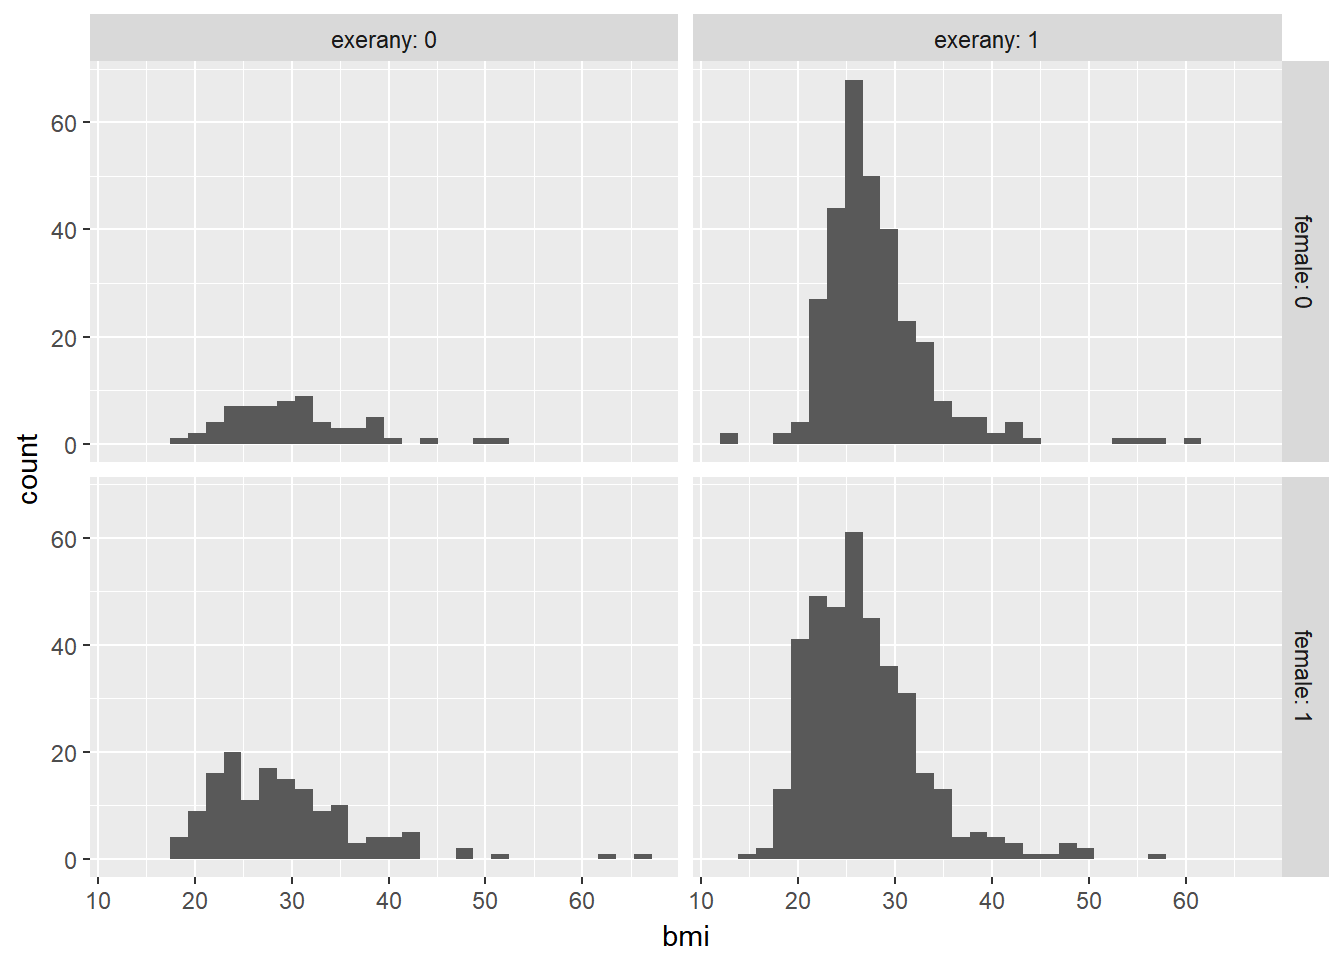
\includegraphics{bookdown-demo_files/figure-latex/c2_smartcle2_plot_bmi_hist_by_female_exerany-1.pdf}

or maybe boxplots?

\begin{Shaded}
\begin{Highlighting}[]
\KeywordTok{ggplot}\NormalTok{(smartcle2, }\KeywordTok{aes}\NormalTok{(}\DataTypeTok{x =} \KeywordTok{factor}\NormalTok{(female), }\DataTypeTok{y =}\NormalTok{ bmi)) }\OperatorTok{+}
\StringTok{    }\KeywordTok{geom_boxplot}\NormalTok{() }\OperatorTok{+}
\StringTok{    }\KeywordTok{facet_wrap}\NormalTok{(}\OperatorTok{~}\StringTok{ }\NormalTok{exerany, }\DataTypeTok{labeller =}\NormalTok{ label_both)}
\end{Highlighting}
\end{Shaded}

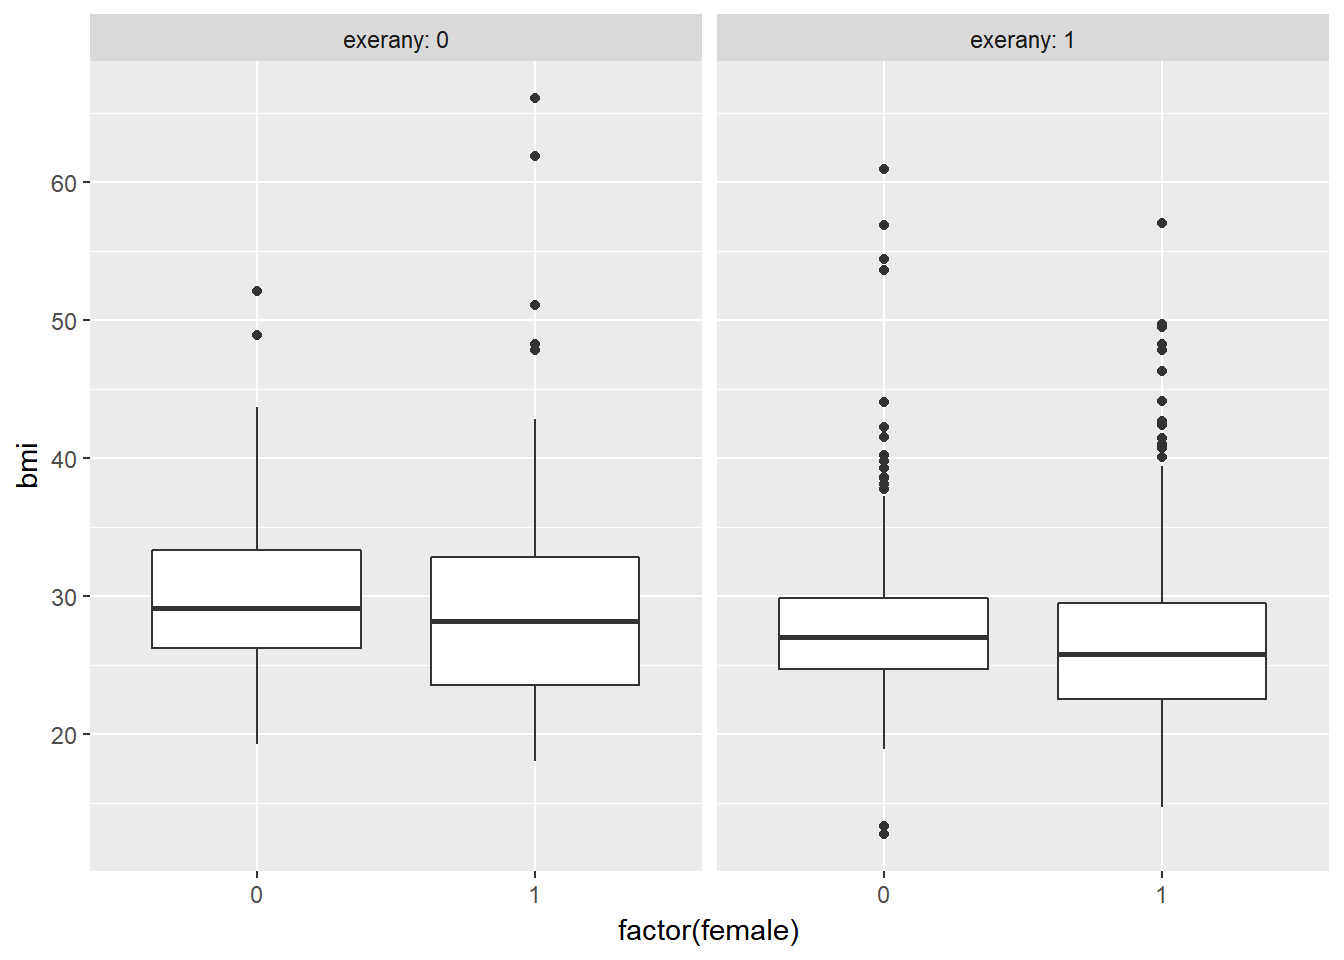
\includegraphics{bookdown-demo_files/figure-latex/c2_smartcle2_plot_bmi_box_by_female_exerany-1.pdf}

\begin{Shaded}
\begin{Highlighting}[]
\KeywordTok{ggplot}\NormalTok{(smartcle2, }\KeywordTok{aes}\NormalTok{(}\DataTypeTok{x =}\NormalTok{ female, }\DataTypeTok{y =}\NormalTok{ bmi))}\OperatorTok{+}
\StringTok{    }\KeywordTok{geom_point}\NormalTok{(}\DataTypeTok{size =} \DecValTok{3}\NormalTok{, }\DataTypeTok{alpha =} \FloatTok{0.2}\NormalTok{) }\OperatorTok{+}
\StringTok{    }\KeywordTok{theme_bw}\NormalTok{() }\OperatorTok{+}
\StringTok{    }\KeywordTok{facet_wrap}\NormalTok{(}\OperatorTok{~}\StringTok{ }\NormalTok{exerany, }\DataTypeTok{labeller =}\NormalTok{ label_both)}
\end{Highlighting}
\end{Shaded}

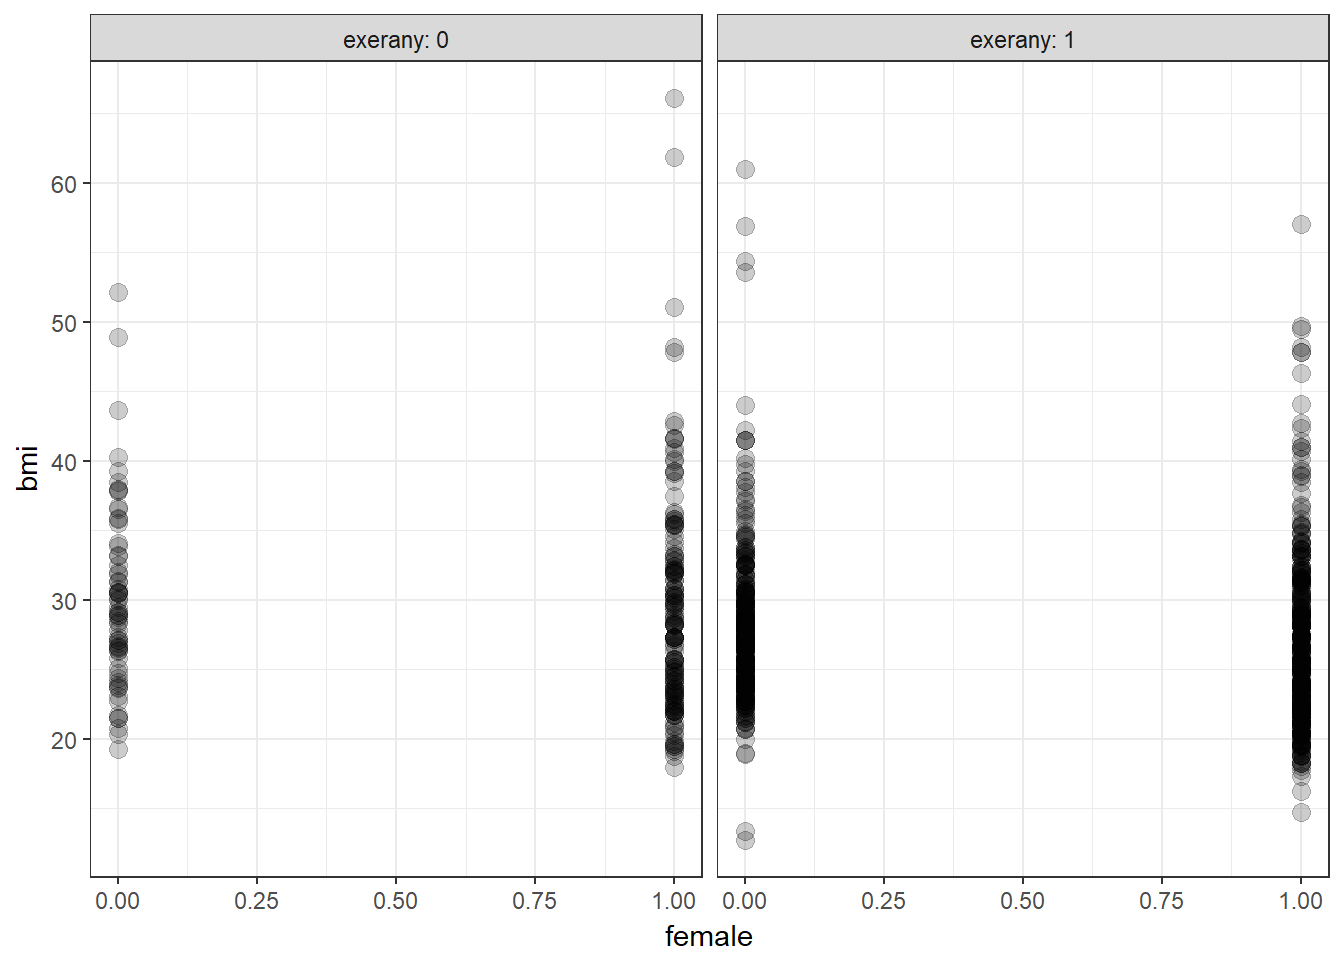
\includegraphics{bookdown-demo_files/figure-latex/c2_smartcle2_plot_bmi_points_by_female_exerany-1.pdf}

OK. Let's try fitting a model.

\begin{Shaded}
\begin{Highlighting}[]
\NormalTok{c2_m2 <-}\StringTok{ }\KeywordTok{lm}\NormalTok{(bmi }\OperatorTok{~}\StringTok{ }\NormalTok{female }\OperatorTok{+}\StringTok{ }\NormalTok{exerany, }\DataTypeTok{data =}\NormalTok{ smartcle2)}
\NormalTok{c2_m2}
\end{Highlighting}
\end{Shaded}

\begin{verbatim}

Call:
lm(formula = bmi ~ female + exerany, data = smartcle2)

Coefficients:
(Intercept)       female      exerany  
     30.334       -1.095       -2.384  
\end{verbatim}

This new model predicts only four predicted values:

\begin{itemize}
\tightlist
\item
  \texttt{bmi} = 30.334 if the subject is male and did not exercise (so
  \texttt{female} = 0 and \texttt{exerany} = 0)
\item
  \texttt{bmi} = 30.334 - 1.095 = 29.239 if the subject is female and
  did not exercise (\texttt{female} = 1 and \texttt{exerany} = 0)
\item
  \texttt{bmi} = 30.334 - 2.384 = 27.950 if the subject is male and
  exercised (so \texttt{female} = 0 and \texttt{exerany} = 1), and,
  finally
\item
  \texttt{bmi} = 30.334 - 1.095 - 2.384 = 26.855 if the subject is
  female and exercised (so both \texttt{female} and \texttt{exerany} =
  1).
\end{itemize}

For those who did not exercise, the model is:

\begin{itemize}
\tightlist
\item
  \texttt{bmi} = 30.334 - 1.095 \texttt{female}
\end{itemize}

and for those who did exercise, the model is:

\begin{itemize}
\tightlist
\item
  \texttt{bmi} = 27.95 - 1.095 \texttt{female}
\end{itemize}

Only the intercept of the \texttt{bmi-female} model changes depending on
\texttt{exerany}.

\begin{Shaded}
\begin{Highlighting}[]
\KeywordTok{summary}\NormalTok{(c2_m2)}
\end{Highlighting}
\end{Shaded}

\begin{verbatim}

Call:
lm(formula = bmi ~ female + exerany, data = smartcle2)

Residuals:
    Min      1Q  Median      3Q     Max 
-15.240  -4.091  -1.095   2.602  36.822 

Coefficients:
            Estimate Std. Error t value Pr(>|t|)    
(Intercept)  30.3335     0.5231   57.99  < 2e-16 ***
female       -1.0952     0.4262   -2.57   0.0103 *  
exerany      -2.3836     0.4965   -4.80 1.86e-06 ***
---
Signif. codes:  0 '***' 0.001 '**' 0.01 '*' 0.05 '.' 0.1 ' ' 1

Residual standard error: 6.239 on 893 degrees of freedom
Multiple R-squared:  0.02939,   Adjusted R-squared:  0.02722 
F-statistic: 13.52 on 2 and 893 DF,  p-value: 1.641e-06
\end{verbatim}

\begin{Shaded}
\begin{Highlighting}[]
\KeywordTok{confint}\NormalTok{(c2_m2)}
\end{Highlighting}
\end{Shaded}

\begin{verbatim}
                2.5 %     97.5 %
(Intercept) 29.306846 31.3602182
female      -1.931629 -0.2588299
exerany     -3.358156 -1.4090777
\end{verbatim}

The slopes of both \texttt{female} and \texttt{exerany} have confidence
intervals that are completely below zero, indicating that both
\texttt{female} sex and \texttt{exerany} appear to be associated with
reductions in \texttt{bmi}.

The R\textsuperscript{2} value suggests that just under 3\% of the
variation in \texttt{bmi} is accounted for by this ANOVA model.

In fact, this regression (on two binary indicator variables) is simply a
two-way ANOVA model without an interaction term.

\begin{Shaded}
\begin{Highlighting}[]
\KeywordTok{anova}\NormalTok{(c2_m2)}
\end{Highlighting}
\end{Shaded}

\begin{verbatim}
Analysis of Variance Table

Response: bmi
           Df Sum Sq Mean Sq F value    Pr(>F)    
female      1    156  155.61  3.9977   0.04586 *  
exerany     1    897  896.93 23.0435 1.856e-06 ***
Residuals 893  34759   38.92                      
---
Signif. codes:  0 '***' 0.001 '**' 0.01 '*' 0.05 '.' 0.1 ' ' 1
\end{verbatim}

\section{\texorpdfstring{\texttt{c2\_m3}: Adding the interaction term
(Two-way ANOVA with
interaction)}{c2\_m3: Adding the interaction term (Two-way ANOVA with interaction)}}\label{c2_m3-adding-the-interaction-term-two-way-anova-with-interaction}

Suppose we want to let the effect of \texttt{female} vary depending on
the \texttt{exerany} status. Then we need to incorporate an interaction
term in our model.

\begin{Shaded}
\begin{Highlighting}[]
\NormalTok{c2_m3 <-}\StringTok{ }\KeywordTok{lm}\NormalTok{(bmi }\OperatorTok{~}\StringTok{ }\NormalTok{female }\OperatorTok{*}\StringTok{ }\NormalTok{exerany, }\DataTypeTok{data =}\NormalTok{ smartcle2)}
\NormalTok{c2_m3}
\end{Highlighting}
\end{Shaded}

\begin{verbatim}

Call:
lm(formula = bmi ~ female * exerany, data = smartcle2)

Coefficients:
   (Intercept)          female         exerany  female:exerany  
       30.1359         -0.8104         -2.1450         -0.3592  
\end{verbatim}

So, for example, for a male who exercises, this model predicts

\begin{itemize}
\tightlist
\item
  \texttt{bmi} = 30.136 - 0.810 (0) - 2.145 (1) - 0.359 (0)(1) = 30.136
  - 2.145 = 27.991
\end{itemize}

And for a female who exercises, the model predicts

\begin{itemize}
\tightlist
\item
  \texttt{bmi} = 30.136 - 0.810 (1) - 2.145 (1) - 0.359 (1)(1) = 30.136
  - 0.810 - 2.145 - 0.359 = 26.822
\end{itemize}

For those who did not exercise, the model is:

\begin{itemize}
\tightlist
\item
  \texttt{bmi} = 30.136 - 0.81 \texttt{female}
\end{itemize}

But for those who did exercise, the model is:

\begin{itemize}
\tightlist
\item
  \texttt{bmi} = (30.136 - 2.145) + (-0.810 + (-0.359)) \texttt{female},
  or ,,,
\item
  \texttt{bmi} = 27.991 - 1.169 \texttt{female}
\end{itemize}

Now, both the slope and the intercept of the \texttt{bmi-female} model
change depending on \texttt{exerany}.

\begin{Shaded}
\begin{Highlighting}[]
\KeywordTok{summary}\NormalTok{(c2_m3)}
\end{Highlighting}
\end{Shaded}

\begin{verbatim}

Call:
lm(formula = bmi ~ female * exerany, data = smartcle2)

Residuals:
    Min      1Q  Median      3Q     Max 
-15.281  -4.101  -1.061   2.566  36.734 

Coefficients:
               Estimate Std. Error t value Pr(>|t|)    
(Intercept)     30.1359     0.7802  38.624   <2e-16 ***
female          -0.8104     0.9367  -0.865   0.3872    
exerany         -2.1450     0.8575  -2.501   0.0125 *  
female:exerany  -0.3592     1.0520  -0.341   0.7328    
---
Signif. codes:  0 '***' 0.001 '**' 0.01 '*' 0.05 '.' 0.1 ' ' 1

Residual standard error: 6.242 on 892 degrees of freedom
Multiple R-squared:  0.02952,   Adjusted R-squared:  0.02625 
F-statistic: 9.044 on 3 and 892 DF,  p-value: 6.669e-06
\end{verbatim}

\begin{Shaded}
\begin{Highlighting}[]
\KeywordTok{confint}\NormalTok{(c2_m3)}
\end{Highlighting}
\end{Shaded}

\begin{verbatim}
                   2.5 %     97.5 %
(Intercept)    28.604610 31.6672650
female         -2.648893  1.0280526
exerany        -3.827886 -0.4620407
female:exerany -2.423994  1.7055248
\end{verbatim}

In fact, this regression (on two binary indicator variables and a
product term) is simply a two-way ANOVA model with an interaction term.

\begin{Shaded}
\begin{Highlighting}[]
\KeywordTok{anova}\NormalTok{(c2_m3)}
\end{Highlighting}
\end{Shaded}

\begin{verbatim}
Analysis of Variance Table

Response: bmi
                Df Sum Sq Mean Sq F value    Pr(>F)    
female           1    156  155.61  3.9938   0.04597 *  
exerany          1    897  896.93 23.0207 1.878e-06 ***
female:exerany   1      5    4.54  0.1166   0.73283    
Residuals      892  34754   38.96                      
---
Signif. codes:  0 '***' 0.001 '**' 0.01 '*' 0.05 '.' 0.1 ' ' 1
\end{verbatim}

The interaction term doesn't change very much here. Its uncertainty
interval includes zero, and the overall model still accounts for just
under 3\% of the variation in \texttt{bmi}.

\section{\texorpdfstring{\texttt{c2\_m4}: Using \texttt{female} and
\texttt{sleephrs} in a model for
\texttt{bmi}}{c2\_m4: Using female and sleephrs in a model for bmi}}\label{c2_m4-using-female-and-sleephrs-in-a-model-for-bmi}

\begin{Shaded}
\begin{Highlighting}[]
\KeywordTok{ggplot}\NormalTok{(smartcle2, }\KeywordTok{aes}\NormalTok{(}\DataTypeTok{x =}\NormalTok{ sleephrs, }\DataTypeTok{y =}\NormalTok{ bmi, }\DataTypeTok{color =} \KeywordTok{factor}\NormalTok{(female))) }\OperatorTok{+}
\StringTok{    }\KeywordTok{geom_point}\NormalTok{() }\OperatorTok{+}\StringTok{ }
\StringTok{    }\KeywordTok{guides}\NormalTok{(}\DataTypeTok{col =} \OtherTok{FALSE}\NormalTok{) }\OperatorTok{+}
\StringTok{    }\KeywordTok{geom_smooth}\NormalTok{(}\DataTypeTok{method =} \StringTok{"lm"}\NormalTok{, }\DataTypeTok{se =} \OtherTok{FALSE}\NormalTok{) }\OperatorTok{+}
\StringTok{    }\KeywordTok{facet_wrap}\NormalTok{(}\OperatorTok{~}\StringTok{ }\NormalTok{female, }\DataTypeTok{labeller =}\NormalTok{ label_both) }
\end{Highlighting}
\end{Shaded}

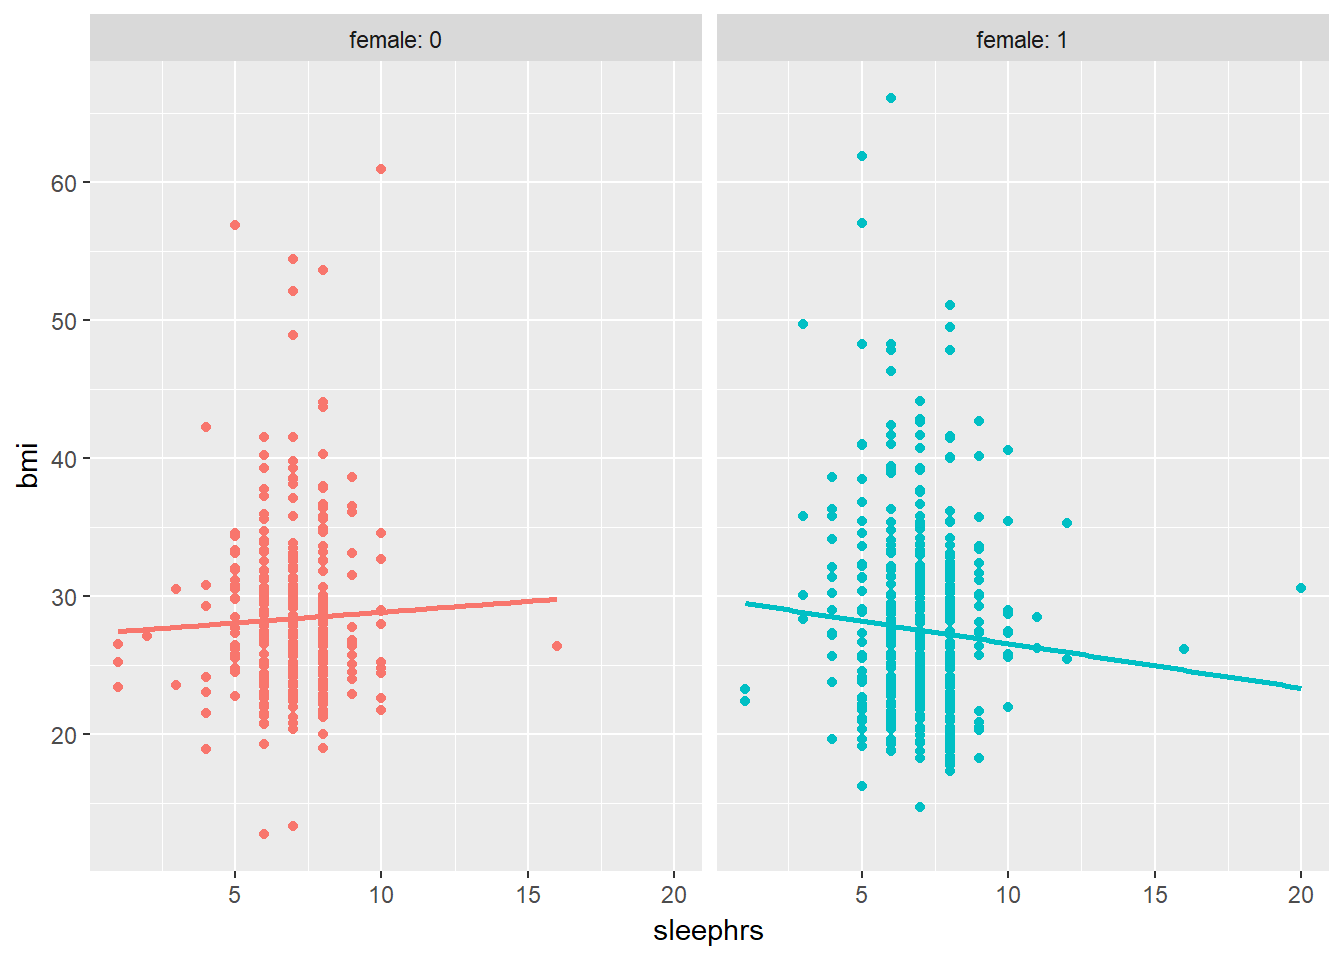
\includegraphics{bookdown-demo_files/figure-latex/graph_to_set_up_c2_m4-1.pdf}

Does the difference in slopes of \texttt{bmi} and \texttt{sleephrs} for
males and females appear to be substantial and important?

\begin{Shaded}
\begin{Highlighting}[]
\NormalTok{c2_m4 <-}\StringTok{ }\KeywordTok{lm}\NormalTok{(bmi }\OperatorTok{~}\StringTok{ }\NormalTok{female }\OperatorTok{*}\StringTok{ }\NormalTok{sleephrs, }\DataTypeTok{data =}\NormalTok{ smartcle2)}

\KeywordTok{summary}\NormalTok{(c2_m4)}
\end{Highlighting}
\end{Shaded}

\begin{verbatim}

Call:
lm(formula = bmi ~ female * sleephrs, data = smartcle2)

Residuals:
    Min      1Q  Median      3Q     Max 
-15.498  -4.179  -1.035   2.830  38.204 

Coefficients:
                Estimate Std. Error t value Pr(>|t|)    
(Intercept)      27.2661     1.6320  16.707   <2e-16 ***
female            2.5263     2.0975   1.204    0.229    
sleephrs          0.1569     0.2294   0.684    0.494    
female:sleephrs  -0.4797     0.2931  -1.636    0.102    
---
Signif. codes:  0 '***' 0.001 '**' 0.01 '*' 0.05 '.' 0.1 ' ' 1

Residual standard error: 6.31 on 892 degrees of freedom
Multiple R-squared:  0.008341,  Adjusted R-squared:  0.005006 
F-statistic: 2.501 on 3 and 892 DF,  p-value: 0.05818
\end{verbatim}

Does it seem as though the addition of \texttt{sleephrs} has improved
our model substantially over a model with \texttt{female} alone (which,
you recall, was \texttt{c2\_m1})?

Since the \texttt{c2\_m4} model contains the \texttt{c2\_m1} model's
predictors as a subset and the outcome is the same for each model, we
consider the models \emph{nested} and have some extra tools available to
compare them.

\begin{itemize}
\tightlist
\item
  I might start by looking at the basic summaries for each model.
\end{itemize}

\begin{Shaded}
\begin{Highlighting}[]
\KeywordTok{glance}\NormalTok{(c2_m4)}
\end{Highlighting}
\end{Shaded}

\begin{verbatim}
    r.squared adj.r.squared    sigma statistic    p.value df    logLik
1 0.008341404   0.005006229 6.309685   2.50104 0.05818038  4 -2919.873
       AIC      BIC deviance df.residual
1 5849.747 5873.736 35512.42         892
\end{verbatim}

\begin{Shaded}
\begin{Highlighting}[]
\KeywordTok{glance}\NormalTok{(c2_m1)}
\end{Highlighting}
\end{Shaded}

\begin{verbatim}
    r.squared adj.r.squared   sigma statistic    p.value df    logLik
1 0.004345169   0.003231461 6.31531  3.901534 0.04854928  2 -2921.675
      AIC      BIC deviance df.residual
1 5849.35 5863.744 35655.53         894
\end{verbatim}

\begin{itemize}
\tightlist
\item
  The R\textsuperscript{2} is twice as large for the model with
  \texttt{sleephrs}, but still very tiny.
\item
  The \emph{p} value for the global ANOVA test is actually less
  significant in \texttt{c2\_m4} than in \texttt{c2\_m1}.
\item
  Smaller AIC and smaller BIC statistics are more desirable. Here,
  there's little to choose from, but \texttt{c2\_m1} is a little better
  on each standard.
\item
  We might also consider a significance test by looking at an ANOVA
  model comparison. This is only appropriate because \texttt{c2\_m1} is
  nested in \texttt{c2\_m4}.
\end{itemize}

\begin{Shaded}
\begin{Highlighting}[]
\KeywordTok{anova}\NormalTok{(c2_m4, c2_m1)}
\end{Highlighting}
\end{Shaded}

\begin{verbatim}
Analysis of Variance Table

Model 1: bmi ~ female * sleephrs
Model 2: bmi ~ female
  Res.Df   RSS Df Sum of Sq      F Pr(>F)
1    892 35512                           
2    894 35656 -2   -143.11 1.7973 0.1663
\end{verbatim}

The addition of the \texttt{sleephrs} term picked up 143 in the sum of
squares column, at a cost of two degrees of freedom, yielding a \emph{p}
value of 0.166, suggesting that this isn't a significant improvement
over the model that just did a t-test on \texttt{female}.

\section{Making Predictions with a Linear Regression
Model}\label{making-predictions-with-a-linear-regression-model}

Recall model 4, which yields predictions for body mass index on the
basis of the main effects of sex (\texttt{female}) and hours of sleep
(\texttt{sleephrs}) and their interaction.

\begin{Shaded}
\begin{Highlighting}[]
\NormalTok{c2_m4}
\end{Highlighting}
\end{Shaded}

\begin{verbatim}

Call:
lm(formula = bmi ~ female * sleephrs, data = smartcle2)

Coefficients:
    (Intercept)           female         sleephrs  female:sleephrs  
        27.2661           2.5263           0.1569          -0.4797  
\end{verbatim}

\subsection{Fitting an Individual Prediction and 95\% Prediction
Interval}\label{fitting-an-individual-prediction-and-95-prediction-interval}

What do we predict for the \texttt{bmi} of a subject who is
\texttt{female} and gets 8 hours of sleep per night?

\begin{Shaded}
\begin{Highlighting}[]
\NormalTok{c2_new1 <-}\StringTok{ }\KeywordTok{data_frame}\NormalTok{(}\DataTypeTok{female =} \DecValTok{1}\NormalTok{, }\DataTypeTok{sleephrs =} \DecValTok{8}\NormalTok{)}
\KeywordTok{predict}\NormalTok{(c2_m4, }\DataTypeTok{newdata =}\NormalTok{ c2_new1, }\DataTypeTok{interval =} \StringTok{"prediction"}\NormalTok{, }\DataTypeTok{level =} \FloatTok{0.95}\NormalTok{)}
\end{Highlighting}
\end{Shaded}

\begin{verbatim}
       fit     lwr     upr
1 27.21065 14.8107 39.6106
\end{verbatim}

The predicted \texttt{bmi} for this new subject is 27.61. The prediction
interval shows the bounds of a 95\% uncertainty interval for a predicted
\texttt{bmi} for an individual female subject who gets 8 hours of sleep
on average per evening. From the \texttt{predict} function applied to a
linear model, we can get the prediction intervals for any new data
points in this manner.

\subsection{Confidence Interval for an Average
Prediction}\label{confidence-interval-for-an-average-prediction}

\begin{itemize}
\tightlist
\item
  What do we predict for the \textbf{average body mass index of a
  population of subjects} who are female and sleep for 8 hours?
\end{itemize}

\begin{Shaded}
\begin{Highlighting}[]
\KeywordTok{predict}\NormalTok{(c2_m4, }\DataTypeTok{newdata =}\NormalTok{ c2_new1, }\DataTypeTok{interval =} \StringTok{"confidence"}\NormalTok{, }\DataTypeTok{level =} \FloatTok{0.95}\NormalTok{)}
\end{Highlighting}
\end{Shaded}

\begin{verbatim}
       fit      lwr      upr
1 27.21065 26.57328 27.84801
\end{verbatim}

\begin{itemize}
\tightlist
\item
  How does this result compare to the prediction interval?
\end{itemize}

\subsection{Fitting Multiple Individual Predictions to New
Data}\label{fitting-multiple-individual-predictions-to-new-data}

\begin{itemize}
\tightlist
\item
  How does our prediction change for a respondent if they instead get 7,
  or 9 hours of sleep? What if they are male, instead of female?
\end{itemize}

\begin{Shaded}
\begin{Highlighting}[]
\NormalTok{c2_new2 <-}\StringTok{ }\KeywordTok{data_frame}\NormalTok{(}\DataTypeTok{subjectid =} \DecValTok{1001}\OperatorTok{:}\DecValTok{1006}\NormalTok{, }\DataTypeTok{female =} \KeywordTok{c}\NormalTok{(}\DecValTok{1}\NormalTok{, }\DecValTok{1}\NormalTok{, }\DecValTok{1}\NormalTok{, }\DecValTok{0}\NormalTok{, }\DecValTok{0}\NormalTok{, }\DecValTok{0}\NormalTok{), }\DataTypeTok{sleephrs =} \KeywordTok{c}\NormalTok{(}\DecValTok{7}\NormalTok{, }\DecValTok{8}\NormalTok{, }\DecValTok{9}\NormalTok{, }\DecValTok{7}\NormalTok{, }\DecValTok{8}\NormalTok{, }\DecValTok{9}\NormalTok{))}
\NormalTok{pred2 <-}\StringTok{ }\KeywordTok{predict}\NormalTok{(c2_m4, }\DataTypeTok{newdata =}\NormalTok{ c2_new2, }\DataTypeTok{interval =} \StringTok{"prediction"}\NormalTok{, }\DataTypeTok{level =} \FloatTok{0.95}\NormalTok{) }\OperatorTok\StringTok{ }\NormalTok{tbl_df}

\NormalTok{result2 <-}\StringTok{ }\KeywordTok{bind_cols}\NormalTok{(c2_new2, pred2)}
\NormalTok{result2}
\end{Highlighting}
\end{Shaded}

\begin{verbatim}
# A tibble: 6 x 6
  subjectid female sleephrs   fit   lwr   upr
      <int>  <dbl>    <dbl> <dbl> <dbl> <dbl>
1      1001     1.       7.  27.5  15.1  39.9
2      1002     1.       8.  27.2  14.8  39.6
3      1003     1.       9.  26.9  14.5  39.3
4      1004     0.       7.  28.4  16.0  40.8
5      1005     0.       8.  28.5  16.1  40.9
6      1006     0.       9.  28.7  16.2  41.1
\end{verbatim}

The \texttt{result2} tibble contains predictions for each scenario.

\begin{itemize}
\tightlist
\item
  Which has a bigger impact on these predictions and prediction
  intervals? A one category change in \texttt{female} or a one hour
  change in \texttt{sleephrs}?
\end{itemize}

\subsection{Simulation to represent predictive uncertainty in Model
4}\label{simulation-to-represent-predictive-uncertainty-in-model-4}

Suppose we want to predict the \texttt{bmi} of a female subject who
sleeps for eight hours per night. As we have seen, we can do this
automatically for a linear model like this one, using the
\texttt{predict} function applied to the linear model, but a simulation
prediction can also be done. Recall the detail of \texttt{c2\_m4}:

\begin{Shaded}
\begin{Highlighting}[]
\NormalTok{c2_m4}
\end{Highlighting}
\end{Shaded}

\begin{verbatim}

Call:
lm(formula = bmi ~ female * sleephrs, data = smartcle2)

Coefficients:
    (Intercept)           female         sleephrs  female:sleephrs  
        27.2661           2.5263           0.1569          -0.4797  
\end{verbatim}

\begin{Shaded}
\begin{Highlighting}[]
\KeywordTok{glance}\NormalTok{(c2_m4)}
\end{Highlighting}
\end{Shaded}

\begin{verbatim}
    r.squared adj.r.squared    sigma statistic    p.value df    logLik
1 0.008341404   0.005006229 6.309685   2.50104 0.05818038  4 -2919.873
       AIC      BIC deviance df.residual
1 5849.747 5873.736 35512.42         892
\end{verbatim}

We see that the residual standard error for our \texttt{bmi} predictions
with this model is 6.31.

For a female respondent sleeping eight hours, recall that our point
estimate (predicted value) of \texttt{bmi} is 27.21

\begin{Shaded}
\begin{Highlighting}[]
\KeywordTok{predict}\NormalTok{(c2_m4, }\DataTypeTok{newdata =}\NormalTok{ c2_new1, }\DataTypeTok{interval =} \StringTok{"prediction"}\NormalTok{, }\DataTypeTok{level =} \FloatTok{0.95}\NormalTok{)}
\end{Highlighting}
\end{Shaded}

\begin{verbatim}
       fit     lwr     upr
1 27.21065 14.8107 39.6106
\end{verbatim}

The standard deviation is 6.31, so we could summarize the predictive
distribution with a command that tells R to draw 1000 random numbers
from a normal distribution with mean 27.21 and standard deviation 6.31.
Let's summarize that and get a quick picture.

\begin{Shaded}
\begin{Highlighting}[]
\KeywordTok{set.seed}\NormalTok{(}\DecValTok{432094}\NormalTok{)}
\NormalTok{pred.sim <-}\StringTok{ }\KeywordTok{rnorm}\NormalTok{(}\DecValTok{1000}\NormalTok{, }\FloatTok{27.21}\NormalTok{, }\FloatTok{6.31}\NormalTok{)}
\KeywordTok{hist}\NormalTok{(pred.sim, }\DataTypeTok{col =} \StringTok{"royalblue"}\NormalTok{)}
\end{Highlighting}
\end{Shaded}

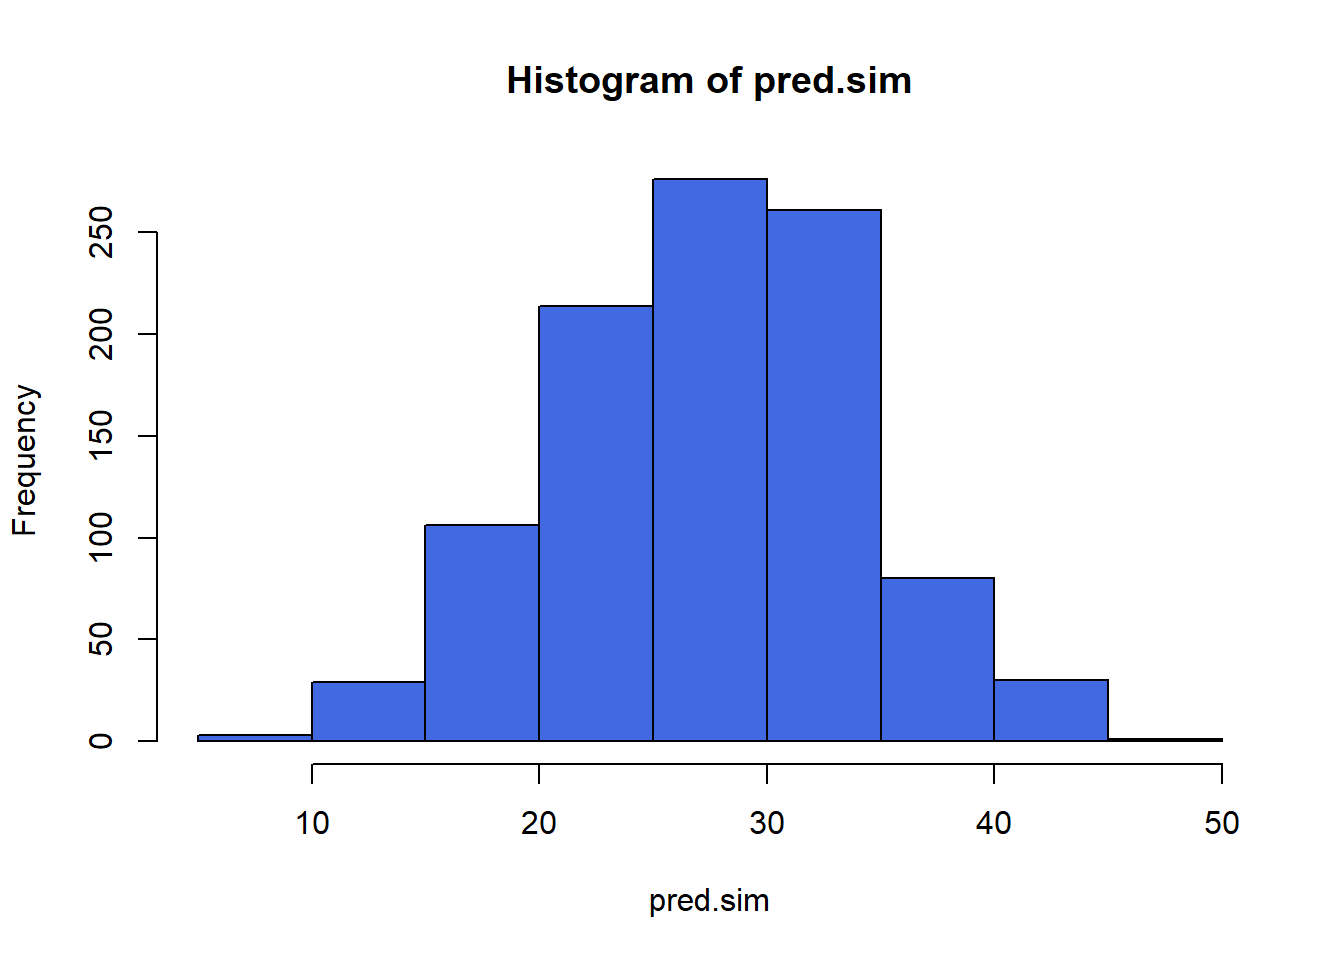
\includegraphics{bookdown-demo_files/figure-latex/unnamed-chunk-10-1.pdf}

\begin{Shaded}
\begin{Highlighting}[]
\KeywordTok{mean}\NormalTok{(pred.sim)}
\end{Highlighting}
\end{Shaded}

\begin{verbatim}
[1] 27.41856
\end{verbatim}

\begin{Shaded}
\begin{Highlighting}[]
\KeywordTok{quantile}\NormalTok{(pred.sim, }\KeywordTok{c}\NormalTok{(}\FloatTok{0.025}\NormalTok{, }\FloatTok{0.975}\NormalTok{))}
\end{Highlighting}
\end{Shaded}

\begin{verbatim}
    2.5%    97.5% 
14.48487 40.16778 
\end{verbatim}

How do these results compare to the prediction interval of (14.81,
39.61) that we generated earlier?

\section{Centering the model}\label{centering-the-model}

Our model \texttt{c2\_m4} has four predictors (the constant,
\texttt{sleephrs}, \texttt{female} and their interaction) but just two
inputs (\texttt{female} and \texttt{sleephrs}.) If we \textbf{center}
the quantitative input \texttt{sleephrs} before building the model, we
get a more interpretable interaction term.

\begin{Shaded}
\begin{Highlighting}[]
\NormalTok{smartcle2_c <-}\StringTok{ }\NormalTok{smartcle2 }\OperatorTok
\StringTok{    }\KeywordTok{mutate}\NormalTok{(}\DataTypeTok{sleephrs_c =}\NormalTok{ sleephrs }\OperatorTok{-}\StringTok{ }\KeywordTok{mean}\NormalTok{(sleephrs))}

\NormalTok{c2_m4_c <-}\StringTok{ }\KeywordTok{lm}\NormalTok{(bmi }\OperatorTok{~}\StringTok{ }\NormalTok{female }\OperatorTok{*}\StringTok{ }\NormalTok{sleephrs_c, }\DataTypeTok{data =}\NormalTok{ smartcle2_c)}

\KeywordTok{summary}\NormalTok{(c2_m4_c)}
\end{Highlighting}
\end{Shaded}

\begin{verbatim}

Call:
lm(formula = bmi ~ female * sleephrs_c, data = smartcle2_c)

Residuals:
    Min      1Q  Median      3Q     Max 
-15.498  -4.179  -1.035   2.830  38.204 

Coefficients:
                  Estimate Std. Error t value Pr(>|t|)    
(Intercept)        28.3681     0.3274  86.658   <2e-16 ***
female             -0.8420     0.4280  -1.967   0.0495 *  
sleephrs_c          0.1569     0.2294   0.684   0.4940    
female:sleephrs_c  -0.4797     0.2931  -1.636   0.1021    
---
Signif. codes:  0 '***' 0.001 '**' 0.01 '*' 0.05 '.' 0.1 ' ' 1

Residual standard error: 6.31 on 892 degrees of freedom
Multiple R-squared:  0.008341,  Adjusted R-squared:  0.005006 
F-statistic: 2.501 on 3 and 892 DF,  p-value: 0.05818
\end{verbatim}

What has changed as compared to the original \texttt{c2\_m4}?

\begin{itemize}
\tightlist
\item
  Our original model was \texttt{bmi} = 27.26 + 2.53 \texttt{female} +
  0.16 \texttt{sleephrs} - 0.48 \texttt{female} x \texttt{sleephrs}
\item
  Our new model is \texttt{bmi} = 28.37 - 0.84 \texttt{female} + 0.16
  centered \texttt{sleephrs} - 0.48 \texttt{female} x centered
  \texttt{sleephrs}.
\end{itemize}

So our new model on centered data is:

\begin{itemize}
\tightlist
\item
  28.37 + 0.16 centered \texttt{sleephrs\_c} for male subjects, and
\item
  (28.37 - 0.84) + (0.16 - 0.48) centered \texttt{sleephrs\_c}, or 27.53
  - 0.32 centered \texttt{sleephrs\_c} for female subjects.
\end{itemize}

In our new (centered \texttt{sleephrs\_c}) model,

\begin{itemize}
\tightlist
\item
  the main effect of \texttt{female} now corresponds to a predictive
  difference (female - male) in \texttt{bmi} with \texttt{sleephrs} at
  its mean value, 7.02 hours,
\item
  the intercept term is now the predicted \texttt{bmi} for a male
  respondent who sleeps an average number of hours, and
\item
  the product term corresponds to the change in the slope of centered
  \texttt{sleephrs\_c} on \texttt{bmi} for a female rather than a male
  subject, while
\item
  the residual standard deviation and the R-squared values remain
  unchanged from the model before centering.
\end{itemize}

\subsection{\texorpdfstring{Plot of Model 4 on Centered
\texttt{sleephrs}:
\texttt{c2\_m4\_c}}{Plot of Model 4 on Centered sleephrs: c2\_m4\_c}}\label{plot-of-model-4-on-centered-sleephrs-c2_m4_c}

\begin{Shaded}
\begin{Highlighting}[]
\KeywordTok{ggplot}\NormalTok{(smartcle2_c, }\KeywordTok{aes}\NormalTok{(}\DataTypeTok{x =}\NormalTok{ sleephrs_c, }\DataTypeTok{y =}\NormalTok{ bmi, }\DataTypeTok{group =}\NormalTok{ female, }\DataTypeTok{col =} \KeywordTok{factor}\NormalTok{(female))) }\OperatorTok{+}
\StringTok{    }\KeywordTok{geom_point}\NormalTok{(}\DataTypeTok{alpha =} \FloatTok{0.5}\NormalTok{, }\DataTypeTok{size =} \DecValTok{2}\NormalTok{) }\OperatorTok{+}
\StringTok{    }\KeywordTok{geom_smooth}\NormalTok{(}\DataTypeTok{method =} \StringTok{"lm"}\NormalTok{, }\DataTypeTok{se =} \OtherTok{FALSE}\NormalTok{) }\OperatorTok{+}
\StringTok{    }\KeywordTok{guides}\NormalTok{(}\DataTypeTok{color =} \OtherTok{FALSE}\NormalTok{) }\OperatorTok{+}
\StringTok{    }\KeywordTok{labs}\NormalTok{(}\DataTypeTok{x =} \StringTok{"Sleep Hours, centered"}\NormalTok{, }\DataTypeTok{y =} \StringTok{"Body Mass Index"}\NormalTok{,}
         \DataTypeTok{title =} \StringTok{"Model `c2_m4` on centered data"}\NormalTok{) }\OperatorTok{+}
\StringTok{    }\KeywordTok{facet_wrap}\NormalTok{(}\OperatorTok{~}\StringTok{ }\NormalTok{female, }\DataTypeTok{labeller =}\NormalTok{ label_both)}
\end{Highlighting}
\end{Shaded}

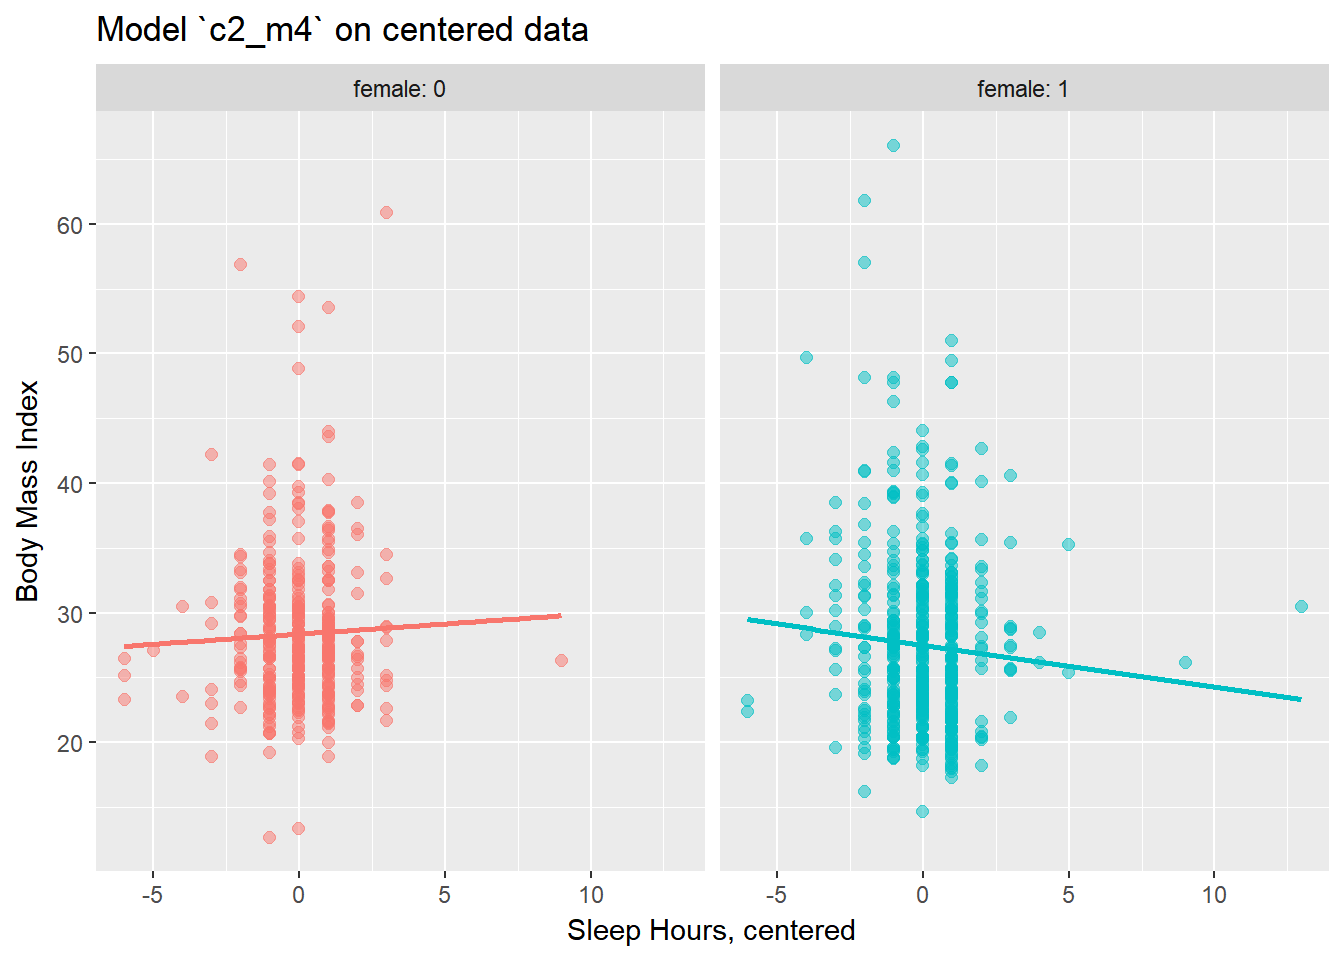
\includegraphics{bookdown-demo_files/figure-latex/unnamed-chunk-12-1.pdf}

\section{Rescaling an input by subtracting the mean and dividing by 2
standard
deviations}\label{rescaling-an-input-by-subtracting-the-mean-and-dividing-by-2-standard-deviations}

Centering helped us interpret the main effects in the regression, but it
still leaves a scaling problem.

\begin{itemize}
\tightlist
\item
  The \texttt{female} coefficient estimate is much larger than that of
  \texttt{sleephrs}, but this is misleading, considering that we are
  comparing the complete change in one variable (sex = female or not) to
  a 1-hour change in average sleep.
\item
  \citet{GelmanHill2007} recommend all continuous predictors be scaled
  by dividing by 2 standard deviations, so that:

  \begin{itemize}
  \tightlist
  \item
    a 1-unit change in the rescaled predictor corresponds to a change
    from 1 standard deviation below the mean, to 1 standard deviation
    above.
  \item
    an unscaled binary (1/0) predictor with 50\% probability of
    occurring will be exactly comparable to a rescaled continuous
    predictor done in this way.
  \end{itemize}
\end{itemize}

\begin{Shaded}
\begin{Highlighting}[]
\NormalTok{smartcle2_rescale <-}\StringTok{ }\NormalTok{smartcle2 }\OperatorTok
\StringTok{    }\KeywordTok{mutate}\NormalTok{(}\DataTypeTok{sleephrs_z =}\NormalTok{ (sleephrs }\OperatorTok{-}\StringTok{ }\KeywordTok{mean}\NormalTok{(sleephrs))}\OperatorTok{/}\NormalTok{(}\DecValTok{2}\OperatorTok{*}\KeywordTok{sd}\NormalTok{(sleephrs)))}
\end{Highlighting}
\end{Shaded}

\subsection{\texorpdfstring{Refitting model \texttt{c2\_m4} to the
rescaled
data}{Refitting model c2\_m4 to the rescaled data}}\label{refitting-model-c2_m4-to-the-rescaled-data}

\begin{Shaded}
\begin{Highlighting}[]
\NormalTok{c2_m4_z <-}\StringTok{ }\KeywordTok{lm}\NormalTok{(bmi }\OperatorTok{~}\StringTok{ }\NormalTok{female }\OperatorTok{*}\StringTok{ }\NormalTok{sleephrs_z, }\DataTypeTok{data =}\NormalTok{ smartcle2_rescale)}

\KeywordTok{summary}\NormalTok{(c2_m4_z)}
\end{Highlighting}
\end{Shaded}

\begin{verbatim}

Call:
lm(formula = bmi ~ female * sleephrs_z, data = smartcle2_rescale)

Residuals:
    Min      1Q  Median      3Q     Max 
-15.498  -4.179  -1.035   2.830  38.204 

Coefficients:
                  Estimate Std. Error t value Pr(>|t|)    
(Intercept)        28.3681     0.3274  86.658   <2e-16 ***
female             -0.8420     0.4280  -1.967   0.0495 *  
sleephrs_z          0.4637     0.6778   0.684   0.4940    
female:sleephrs_z  -1.4173     0.8661  -1.636   0.1021    
---
Signif. codes:  0 '***' 0.001 '**' 0.01 '*' 0.05 '.' 0.1 ' ' 1

Residual standard error: 6.31 on 892 degrees of freedom
Multiple R-squared:  0.008341,  Adjusted R-squared:  0.005006 
F-statistic: 2.501 on 3 and 892 DF,  p-value: 0.05818
\end{verbatim}

\subsection{Interpreting the model on rescaled
data}\label{interpreting-the-model-on-rescaled-data}

What has changed as compared to the original \texttt{c2\_m4}?

\begin{itemize}
\tightlist
\item
  Our original model was \texttt{bmi} = 27.26 + 2.53 \texttt{female} +
  0.16 \texttt{sleephrs} - 0.48 \texttt{female} x \texttt{sleephrs}
\item
  Our model on centered \texttt{sleephrs} was \texttt{bmi} = 28.37 -
  0.84 \texttt{female} + 0.16 centered \texttt{sleephrs\_c} - 0.48
  \texttt{female} x centered \texttt{sleephrs\_c}.
\item
  Our new model on rescaled \texttt{sleephrs} is \texttt{bmi} = 28.37 -
  0.84 \texttt{female} + 0.46 rescaled \texttt{sleephrs\_z} - 1.42
  \texttt{female} x rescaled \texttt{sleephrs\_z}.
\end{itemize}

So our rescaled model is:

\begin{itemize}
\tightlist
\item
  28.37 + 0.46 rescaled \texttt{sleephrs\_z} for male subjects, and
\item
  (28.37 - 0.84) + (0.46 - 1.42) rescaled \texttt{sleephrs\_z}, or 27.53
  - 0.96 rescaled \texttt{sleephrs\_z} for female subjects.
\end{itemize}

In this new rescaled (\texttt{sleephrs\_z}) model, then,

\begin{itemize}
\tightlist
\item
  the main effect of \texttt{female}, -0.84, still corresponds to a
  predictive difference (female - male) in \texttt{bmi} with
  \texttt{sleephrs} at its mean value, 7.02 hours,
\item
  the intercept term is still the predicted \texttt{bmi} for a male
  respondent who sleeps an average number of hours, and
\item
  the residual standard deviation and the R-squared values remain
  unchanged,
\end{itemize}

as before, but now we also have that:

\begin{itemize}
\tightlist
\item
  the coefficient of \texttt{sleephrs\_z} indicates the predictive
  difference in \texttt{bmi} associated with a change in
  \texttt{sleephrs} of 2 standard deviations (from one standard
  deviation below the mean of 7.02 to one standard deviation above
  7.02.)

  \begin{itemize}
  \tightlist
  \item
    Since the standard deviation of \texttt{sleephrs} is 1.48, this
    corresponds to a change from 5.54 hours per night to 8.50 hours per
    night.
  \end{itemize}
\item
  the coefficient of the product term (-1.42) corresponds to the change
  in the coefficient of \texttt{sleephrs\_z} for females as compared to
  males.
\end{itemize}

\subsection{Plot of model on rescaled
data}\label{plot-of-model-on-rescaled-data}

\begin{Shaded}
\begin{Highlighting}[]
\KeywordTok{ggplot}\NormalTok{(smartcle2_rescale, }\KeywordTok{aes}\NormalTok{(}\DataTypeTok{x =}\NormalTok{ sleephrs_z, }\DataTypeTok{y =}\NormalTok{ bmi, }
                              \DataTypeTok{group =}\NormalTok{ female, }\DataTypeTok{col =} \KeywordTok{factor}\NormalTok{(female))) }\OperatorTok{+}
\StringTok{    }\KeywordTok{geom_point}\NormalTok{(}\DataTypeTok{alpha =} \FloatTok{0.5}\NormalTok{) }\OperatorTok{+}
\StringTok{    }\KeywordTok{geom_smooth}\NormalTok{(}\DataTypeTok{method =} \StringTok{"lm"}\NormalTok{, }\DataTypeTok{size =} \FloatTok{1.5}\NormalTok{) }\OperatorTok{+}
\StringTok{    }\KeywordTok{scale_color_discrete}\NormalTok{(}\DataTypeTok{name =} \StringTok{"Is subject female?"}\NormalTok{) }\OperatorTok{+}
\StringTok{    }\KeywordTok{labs}\NormalTok{(}\DataTypeTok{x =} \StringTok{"Sleep Hours, standardized (2 sd)"}\NormalTok{, }\DataTypeTok{y =} \StringTok{"Body Mass Index"}\NormalTok{,}
         \DataTypeTok{title =} \StringTok{"Model `c2_m4_z` on rescaled data"}\NormalTok{)}
\end{Highlighting}
\end{Shaded}

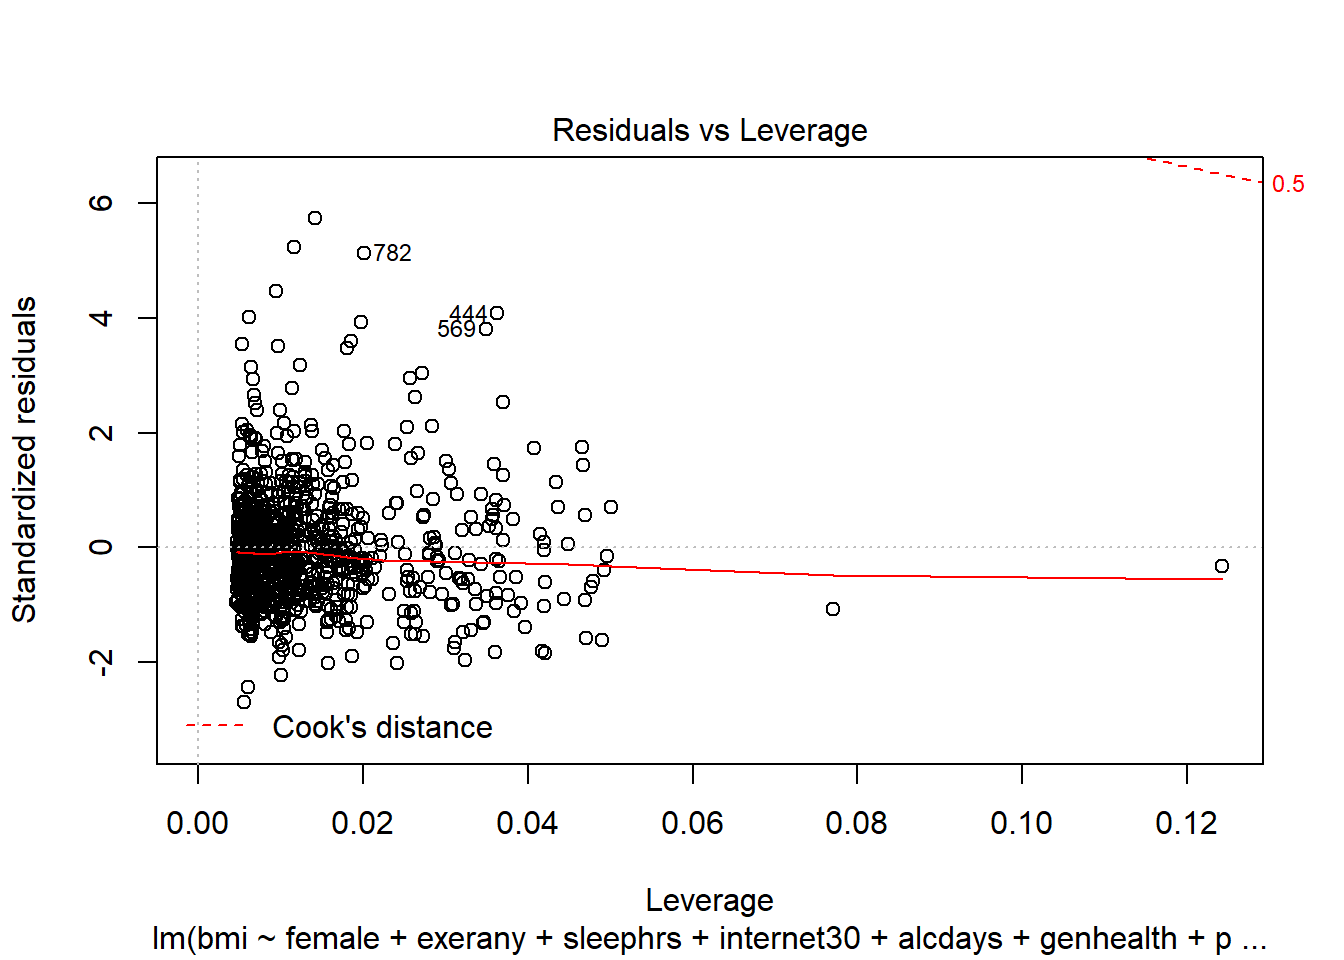
\includegraphics{bookdown-demo_files/figure-latex/unnamed-chunk-14-1.pdf}

\section{\texorpdfstring{\texttt{c2\_m5}: What if we add more
variables?}{c2\_m5: What if we add more variables?}}\label{c2_m5-what-if-we-add-more-variables}

We can boost our R\textsuperscript{2} a bit, to over 5\%, by adding in
two new variables, related to whether or not the subject (in the past 30
days) used the internet, and on how many days the subject drank
alcoholic beverages.

\begin{Shaded}
\begin{Highlighting}[]
\NormalTok{c2_m5 <-}\StringTok{ }\KeywordTok{lm}\NormalTok{(bmi }\OperatorTok{~}\StringTok{ }\NormalTok{female }\OperatorTok{+}\StringTok{ }\NormalTok{exerany }\OperatorTok{+}\StringTok{ }\NormalTok{sleephrs }\OperatorTok{+}\StringTok{ }\NormalTok{internet30 }\OperatorTok{+}\StringTok{ }\NormalTok{alcdays,}
         \DataTypeTok{data =}\NormalTok{ smartcle2)}
\KeywordTok{summary}\NormalTok{(c2_m5)}
\end{Highlighting}
\end{Shaded}

\begin{verbatim}

Call:
lm(formula = bmi ~ female + exerany + sleephrs + internet30 + 
    alcdays, data = smartcle2)

Residuals:
    Min      1Q  Median      3Q     Max 
-16.147  -3.997  -0.856   2.487  35.965 

Coefficients:
            Estimate Std. Error t value Pr(>|t|)    
(Intercept) 30.84066    1.18458  26.035  < 2e-16 ***
female      -1.28801    0.42805  -3.009   0.0027 ** 
exerany     -2.42161    0.49853  -4.858 1.40e-06 ***
sleephrs    -0.14118    0.13988  -1.009   0.3131    
internet30   1.38916    0.54252   2.561   0.0106 *  
alcdays     -0.10460    0.02595  -4.030 6.04e-05 ***
---
Signif. codes:  0 '***' 0.001 '**' 0.01 '*' 0.05 '.' 0.1 ' ' 1

Residual standard error: 6.174 on 890 degrees of freedom
Multiple R-squared:  0.05258,   Adjusted R-squared:  0.04726 
F-statistic: 9.879 on 5 and 890 DF,  p-value: 3.304e-09
\end{verbatim}

\begin{enumerate}
\def\labelenumi{\arabic{enumi}.}
\tightlist
\item
  Here's the ANOVA for this model. What can we study with this?
\end{enumerate}

\begin{Shaded}
\begin{Highlighting}[]
\KeywordTok{anova}\NormalTok{(c2_m5)}
\end{Highlighting}
\end{Shaded}

\begin{verbatim}
Analysis of Variance Table

Response: bmi
            Df Sum Sq Mean Sq F value    Pr(>F)    
female       1    156  155.61  4.0818   0.04365 *  
exerany      1    897  896.93 23.5283 1.453e-06 ***
sleephrs     1     33   32.90  0.8631   0.35313    
internet30   1    178  178.33  4.6779   0.03082 *  
alcdays      1    619  619.26 16.2443 6.044e-05 ***
Residuals  890  33928   38.12                      
---
Signif. codes:  0 '***' 0.001 '**' 0.01 '*' 0.05 '.' 0.1 ' ' 1
\end{verbatim}

\begin{enumerate}
\def\labelenumi{\arabic{enumi}.}
\setcounter{enumi}{1}
\tightlist
\item
  Consider the revised output below. Now what can we study?
\end{enumerate}

\begin{Shaded}
\begin{Highlighting}[]
\KeywordTok{anova}\NormalTok{(}\KeywordTok{lm}\NormalTok{(bmi }\OperatorTok{~}\StringTok{ }\NormalTok{exerany }\OperatorTok{+}\StringTok{ }\NormalTok{internet30 }\OperatorTok{+}\StringTok{ }\NormalTok{alcdays }\OperatorTok{+}\StringTok{ }\NormalTok{female }\OperatorTok{+}\StringTok{ }\NormalTok{sleephrs,}
         \DataTypeTok{data =}\NormalTok{ smartcle2))}
\end{Highlighting}
\end{Shaded}

\begin{verbatim}
Analysis of Variance Table

Response: bmi
            Df Sum Sq Mean Sq F value    Pr(>F)    
exerany      1    795  795.46 20.8664 5.618e-06 ***
internet30   1    212  211.95  5.5599 0.0185925 *  
alcdays      1    486  486.03 12.7496 0.0003752 ***
female       1    351  350.75  9.2010 0.0024891 ** 
sleephrs     1     39   38.83  1.0186 0.3131176    
Residuals  890  33928   38.12                      
---
Signif. codes:  0 '***' 0.001 '**' 0.01 '*' 0.05 '.' 0.1 ' ' 1
\end{verbatim}

\begin{enumerate}
\def\labelenumi{\arabic{enumi}.}
\setcounter{enumi}{2}
\tightlist
\item
  What does the output below let us conclude?
\end{enumerate}

\begin{Shaded}
\begin{Highlighting}[]
\KeywordTok{anova}\NormalTok{(}\KeywordTok{lm}\NormalTok{(bmi }\OperatorTok{~}\StringTok{ }\NormalTok{exerany }\OperatorTok{+}\StringTok{ }\NormalTok{internet30 }\OperatorTok{+}\StringTok{ }\NormalTok{alcdays }\OperatorTok{+}\StringTok{ }\NormalTok{female }\OperatorTok{+}\StringTok{ }\NormalTok{sleephrs, }
         \DataTypeTok{data =}\NormalTok{ smartcle2),}
      \KeywordTok{lm}\NormalTok{(bmi }\OperatorTok{~}\StringTok{ }\NormalTok{exerany }\OperatorTok{+}\StringTok{ }\NormalTok{female }\OperatorTok{+}\StringTok{ }\NormalTok{alcdays, }
         \DataTypeTok{data =}\NormalTok{ smartcle2))}
\end{Highlighting}
\end{Shaded}

\begin{verbatim}
Analysis of Variance Table

Model 1: bmi ~ exerany + internet30 + alcdays + female + sleephrs
Model 2: bmi ~ exerany + female + alcdays
  Res.Df   RSS Df Sum of Sq      F  Pr(>F)  
1    890 33928                              
2    892 34221 -2    -293.2 3.8456 0.02173 *
---
Signif. codes:  0 '***' 0.001 '**' 0.01 '*' 0.05 '.' 0.1 ' ' 1
\end{verbatim}

\begin{enumerate}
\def\labelenumi{\arabic{enumi}.}
\setcounter{enumi}{3}
\tightlist
\item
  What does it mean for the models to be ``nested''?
\end{enumerate}

\section{\texorpdfstring{\texttt{c2\_m6}: Would adding self-reported
health
help?}{c2\_m6: Would adding self-reported health help?}}\label{c2_m6-would-adding-self-reported-health-help}

And we can do even a bit better than that by adding in a
multi-categorical measure: self-reported general health.

\begin{Shaded}
\begin{Highlighting}[]
\NormalTok{c2_m6 <-}\StringTok{ }\KeywordTok{lm}\NormalTok{(bmi }\OperatorTok{~}\StringTok{ }\NormalTok{female }\OperatorTok{+}\StringTok{ }\NormalTok{exerany }\OperatorTok{+}\StringTok{ }\NormalTok{sleephrs }\OperatorTok{+}\StringTok{ }\NormalTok{internet30 }\OperatorTok{+}\StringTok{ }\NormalTok{alcdays }\OperatorTok{+}\StringTok{ }\NormalTok{genhealth,}
         \DataTypeTok{data =}\NormalTok{ smartcle2)}
\KeywordTok{summary}\NormalTok{(c2_m6)}
\end{Highlighting}
\end{Shaded}

\begin{verbatim}

Call:
lm(formula = bmi ~ female + exerany + sleephrs + internet30 + 
    alcdays + genhealth, data = smartcle2)

Residuals:
    Min      1Q  Median      3Q     Max 
-16.331  -3.813  -0.838   2.679  34.166 

Coefficients:
                    Estimate Std. Error t value Pr(>|t|)    
(Intercept)         26.49498    1.31121  20.206  < 2e-16 ***
female              -0.85520    0.41969  -2.038 0.041879 *  
exerany             -1.61968    0.50541  -3.205 0.001400 ** 
sleephrs            -0.12719    0.13613  -0.934 0.350368    
internet30           2.02498    0.53898   3.757 0.000183 ***
alcdays             -0.08431    0.02537  -3.324 0.000925 ***
genhealth2_VeryGood  2.10537    0.59408   3.544 0.000415 ***
genhealth3_Good      4.08245    0.60739   6.721 3.22e-11 ***
genhealth4_Fair      4.99213    0.80178   6.226 7.37e-10 ***
genhealth5_Poor      3.11025    1.12614   2.762 0.005866 ** 
---
Signif. codes:  0 '***' 0.001 '**' 0.01 '*' 0.05 '.' 0.1 ' ' 1

Residual standard error: 5.993 on 886 degrees of freedom
Multiple R-squared:  0.1115,    Adjusted R-squared:  0.1024 
F-statistic: 12.35 on 9 and 886 DF,  p-value: < 2.2e-16
\end{verbatim}

\begin{enumerate}
\def\labelenumi{\arabic{enumi}.}
\item
  If Harry and Marty have the same values of \texttt{female},
  \texttt{exerany}, \texttt{sleephrs}, \texttt{internet30} and
  \texttt{alcdays}, but Harry rates his health as Good, and Marty rates
  his as Fair, then what is the difference in the predictions? Who is
  predicted to have a larger BMI, and by how much?
\item
  What does this normal probability plot of the residuals suggest?
\end{enumerate}

\begin{Shaded}
\begin{Highlighting}[]
\KeywordTok{plot}\NormalTok{(c2_m6, }\DataTypeTok{which =} \DecValTok{2}\NormalTok{)}
\end{Highlighting}
\end{Shaded}

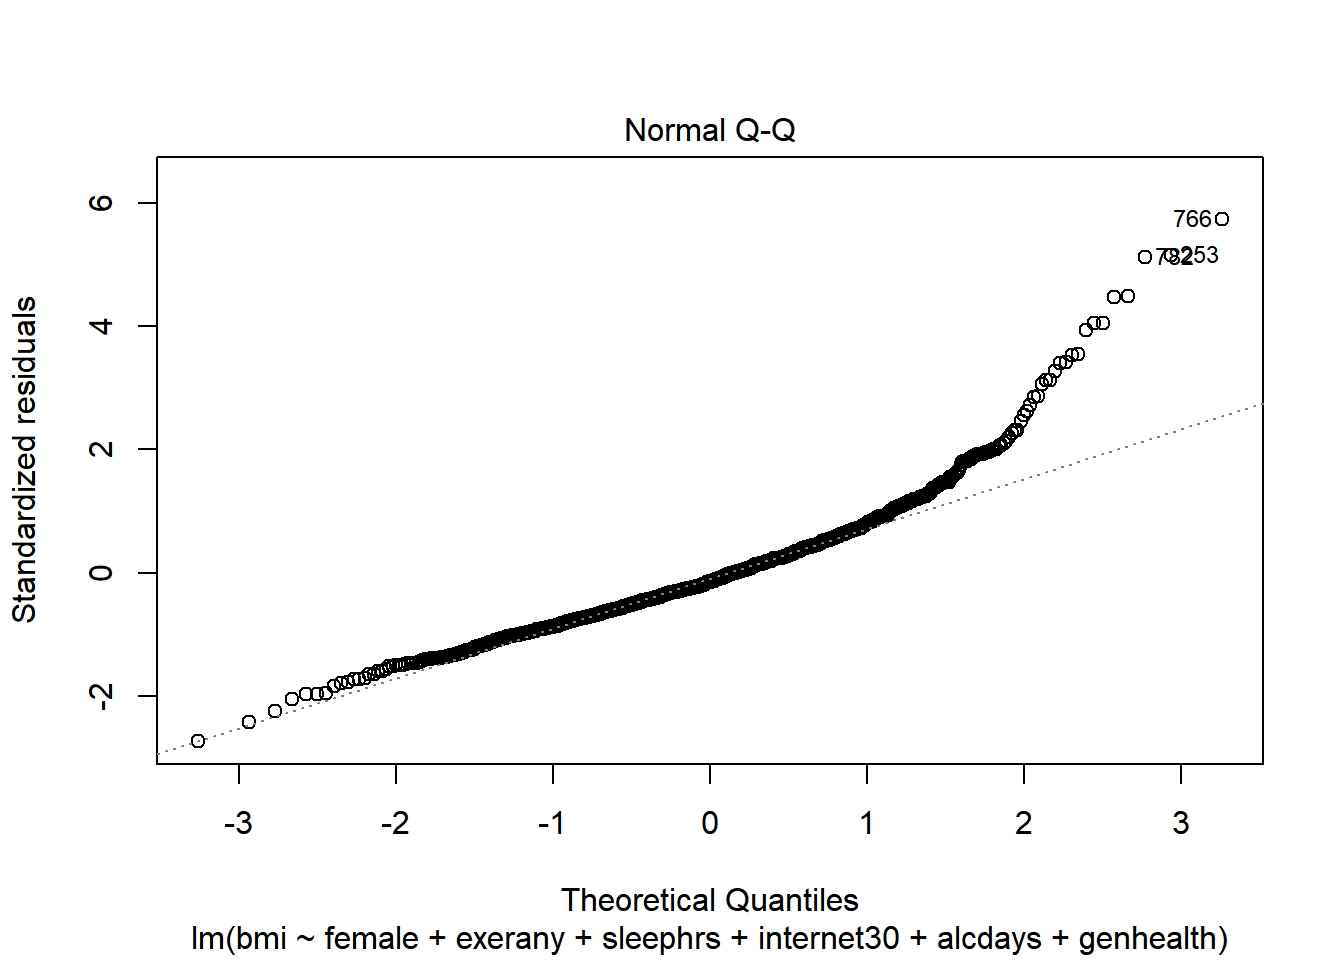
\includegraphics{bookdown-demo_files/figure-latex/c2_m6_residuals_normality-1.pdf}

\section{\texorpdfstring{\texttt{c2\_m7}: What if we added the
\texttt{menthealth}
variable?}{c2\_m7: What if we added the menthealth variable?}}\label{c2_m7-what-if-we-added-the-menthealth-variable}

\begin{Shaded}
\begin{Highlighting}[]
\NormalTok{c2_m7 <-}\StringTok{ }\KeywordTok{lm}\NormalTok{(bmi }\OperatorTok{~}\StringTok{ }\NormalTok{female }\OperatorTok{+}\StringTok{ }\NormalTok{exerany }\OperatorTok{+}\StringTok{ }\NormalTok{sleephrs }\OperatorTok{+}\StringTok{ }\NormalTok{internet30 }\OperatorTok{+}\StringTok{ }\NormalTok{alcdays }\OperatorTok{+}\StringTok{ }
\StringTok{                }\NormalTok{genhealth }\OperatorTok{+}\StringTok{ }\NormalTok{physhealth }\OperatorTok{+}\StringTok{ }\NormalTok{menthealth,}
         \DataTypeTok{data =}\NormalTok{ smartcle2)}

\KeywordTok{summary}\NormalTok{(c2_m7)}
\end{Highlighting}
\end{Shaded}

\begin{verbatim}

Call:
lm(formula = bmi ~ female + exerany + sleephrs + internet30 + 
    alcdays + genhealth + physhealth + menthealth, data = smartcle2)

Residuals:
    Min      1Q  Median      3Q     Max 
-16.060  -3.804  -0.890   2.794  33.972 

Coefficients:
                    Estimate Std. Error t value Pr(>|t|)    
(Intercept)         25.88208    1.31854  19.629  < 2e-16 ***
female              -0.96435    0.41908  -2.301 0.021616 *  
exerany             -1.43171    0.50635  -2.828 0.004797 ** 
sleephrs            -0.08033    0.13624  -0.590 0.555583    
internet30           2.00267    0.53759   3.725 0.000207 ***
alcdays             -0.07997    0.02528  -3.163 0.001614 ** 
genhealth2_VeryGood  2.09533    0.59238   3.537 0.000425 ***
genhealth3_Good      3.90949    0.60788   6.431 2.07e-10 ***
genhealth4_Fair      4.27152    0.83986   5.086 4.47e-07 ***
genhealth5_Poor      1.26021    1.31556   0.958 0.338361    
physhealth           0.06088    0.03005   2.026 0.043064 *  
menthealth           0.06636    0.03177   2.089 0.037021 *  
---
Signif. codes:  0 '***' 0.001 '**' 0.01 '*' 0.05 '.' 0.1 ' ' 1

Residual standard error: 5.964 on 884 degrees of freedom
Multiple R-squared:  0.1219,    Adjusted R-squared:  0.111 
F-statistic: 11.16 on 11 and 884 DF,  p-value: < 2.2e-16
\end{verbatim}

\section{Key Regression Assumptions for Building Effective Prediction
Models}\label{key-regression-assumptions-for-building-effective-prediction-models}

\begin{enumerate}
\def\labelenumi{\arabic{enumi}.}
\tightlist
\item
  Validity - the data you are analyzing should map to the research
  question you are trying to answer.

  \begin{itemize}
  \tightlist
  \item
    The outcome should accurately reflect the phenomenon of interest.
  \item
    The model should include all relevant predictors. (It can be
    difficult to decide which predictors are necessary, and what to do
    with predictors that have large standard errors.)
  \item
    The model should generalize to all of the cases to which it will be
    applied.
  \item
    Can the available data answer our question reliably?
  \end{itemize}
\item
  Additivity and linearity - most important assumption of a regression
  model is that its deterministic component is a linear function of the
  predictors. We often think about transformations in this setting.
\item
  Independence of errors - errors from the prediction line are
  independent of each other
\item
  Equal variance of errors - if this is violated, we can more
  efficiently estimate parameters using \emph{weighted least squares}
  approaches, where each point is weighted inversely proportional to its
  variance, but this doesn't affect the coefficients much, if at all.
\item
  Normality of errors - not generally important for estimating the
  regression line
\end{enumerate}

\subsection{\texorpdfstring{Checking Assumptions in model
\texttt{c2\_m7}}{Checking Assumptions in model c2\_m7}}\label{checking-assumptions-in-model-c2_m7}

\begin{enumerate}
\def\labelenumi{\arabic{enumi}.}
\tightlist
\item
  How does the assumption of linearity behind this model look?
\end{enumerate}

\begin{Shaded}
\begin{Highlighting}[]
\KeywordTok{plot}\NormalTok{(c2_m7, }\DataTypeTok{which =} \DecValTok{1}\NormalTok{)}
\end{Highlighting}
\end{Shaded}

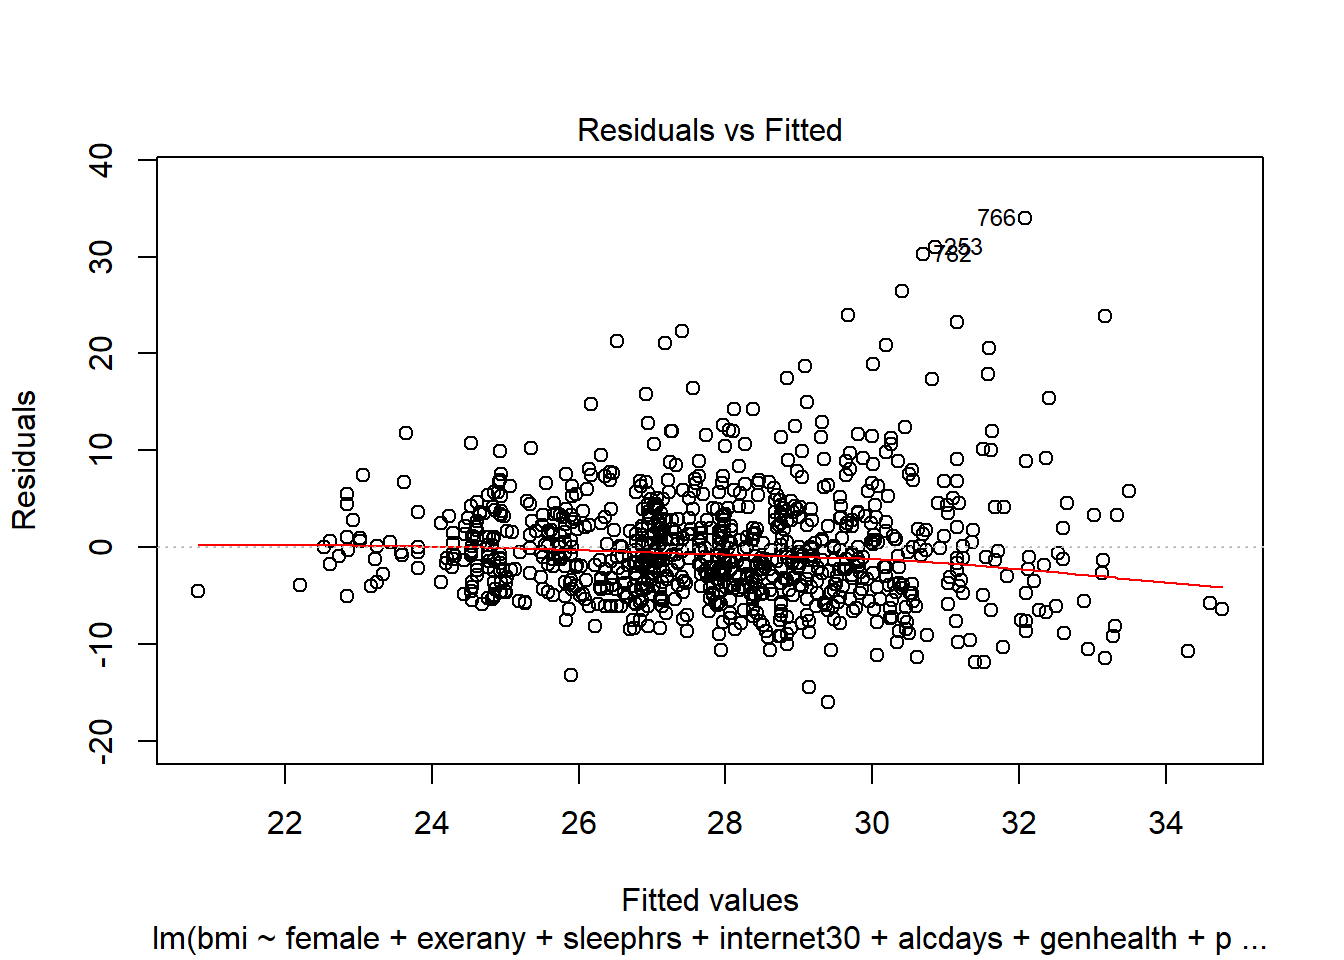
\includegraphics{bookdown-demo_files/figure-latex/residual_plot1_c2_m7-1.pdf}

We see no strong signs of serious non-linearity here. There's no obvious
curve in the plot, for example.

\begin{enumerate}
\def\labelenumi{\arabic{enumi}.}
\setcounter{enumi}{1}
\tightlist
\item
  What can we conclude from the plot below?
\end{enumerate}

\begin{Shaded}
\begin{Highlighting}[]
\KeywordTok{plot}\NormalTok{(c2_m7, }\DataTypeTok{which =} \DecValTok{5}\NormalTok{)}
\end{Highlighting}
\end{Shaded}

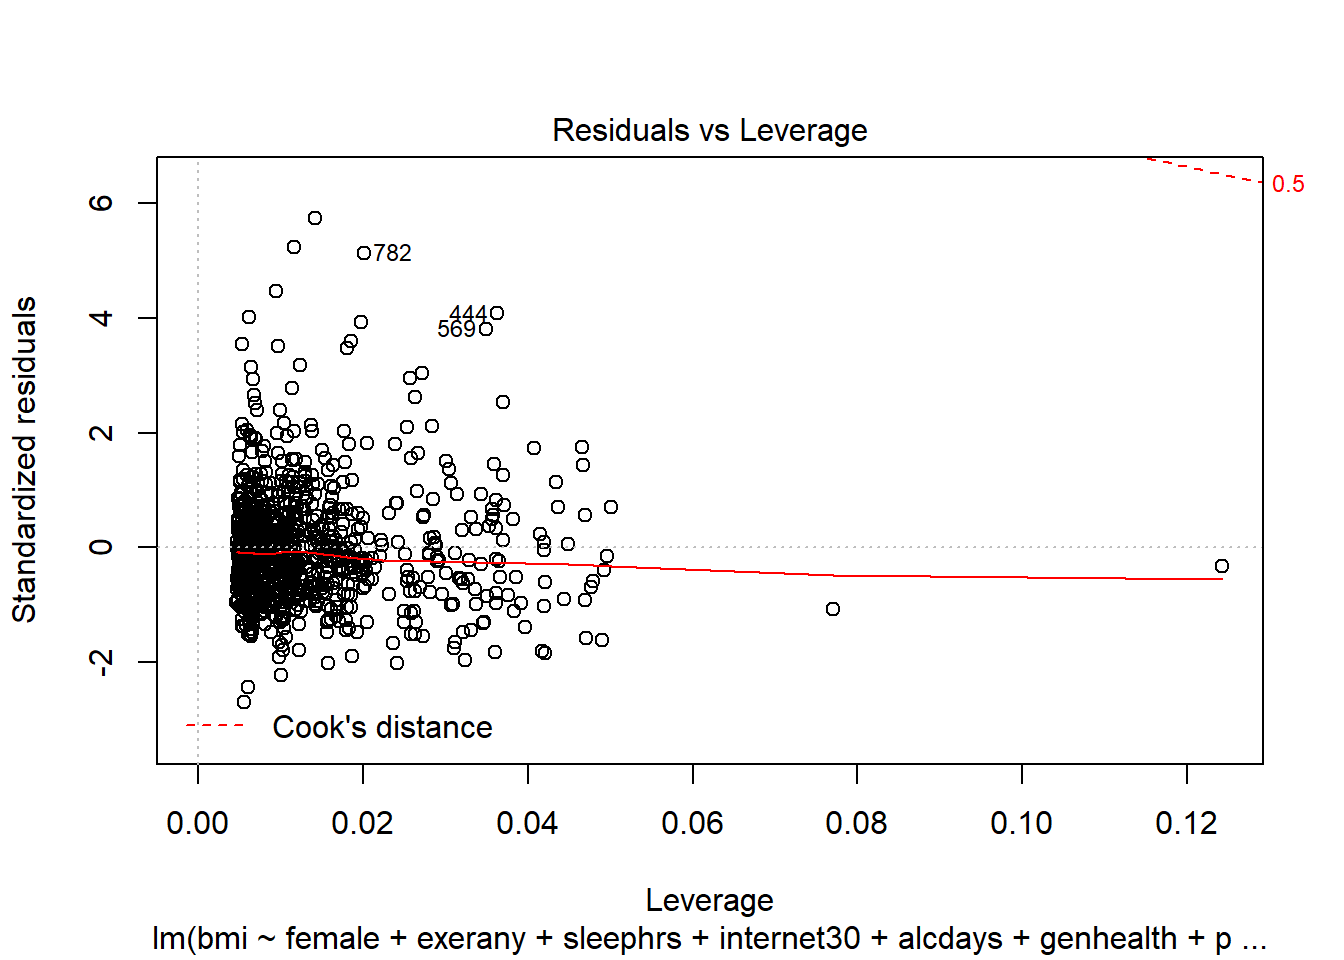
\includegraphics{bookdown-demo_files/figure-latex/residual_plot5_c2_m7-1.pdf}

This plot can help us identify points with large standardized residuals,
large leverage values, and large influence on the model (as indicated by
large values of Cook's distance.) In this case, I see no signs of any
points used in the model with especially large influence, although there
are some poorly fitted points (with especially large standardized
residuals.)

\chapter{Analysis of Variance}\label{analysis-of-variance}

\section{\texorpdfstring{The \texttt{bonding} data: A Designed Dental
Experiment}{The bonding data: A Designed Dental Experiment}}\label{the-bonding-data-a-designed-dental-experiment}

The \texttt{bonding} data describe a designed experiment into the
properties of four different resin types (\texttt{resin} = A, B, C, D)
and two different curing light sources (\texttt{light} = Halogen, LED)
as they relate to the resulting bonding strength (measured in
MPa\footnote{The MPa is defined as the failure load (in Newtons) divided
  by the entire bonded area, in mm\textsuperscript{2}.}) on the surface
of teeth. The source is \citet{Kim2014}.

The experiment involved making measurements of bonding strength under a
total of 80 experimental setups, or runs, with 10 runs completed at each
of the eight combinations of a light source and a resin type. The data
are gathered in the \texttt{bonding.csv} file.

\begin{Shaded}
\begin{Highlighting}[]
\NormalTok{bonding}
\end{Highlighting}
\end{Shaded}

\begin{verbatim}
# A tibble: 80 x 4
   run_ID light   resin strength
   <fct>  <fct>   <fct>    <dbl>
 1 R101   LED     B         12.8
 2 R102   Halogen B         22.2
 3 R103   Halogen B         24.6
 4 R104   LED     A         17.0
 5 R105   LED     C         32.2
 6 R106   Halogen B         27.1
 7 R107   LED     A         23.4
 8 R108   Halogen A         23.5
 9 R109   Halogen D         37.3
10 R110   Halogen A         19.7
# ... with 70 more rows
\end{verbatim}

\section{A One-Factor Analysis of
Variance}\label{a-one-factor-analysis-of-variance}

Suppose we are interested in the distribution of the \texttt{strength}
values for the four different types of \texttt{resin}.

\begin{Shaded}
\begin{Highlighting}[]
\NormalTok{bonding }\OperatorTok\StringTok{ }\KeywordTok{group_by}\NormalTok{(resin) }\OperatorTok\StringTok{ }\KeywordTok{summarize}\NormalTok{(}\DataTypeTok{n =} \KeywordTok{n}\NormalTok{(), }\KeywordTok{mean}\NormalTok{(strength), }\KeywordTok{median}\NormalTok{(strength))}
\end{Highlighting}
\end{Shaded}

\begin{verbatim}
# A tibble: 4 x 4
  resin     n `mean(strength)` `median(strength)`
  <fct> <int>            <dbl>              <dbl>
1 A        20             18.4               18.0
2 B        20             22.2               22.7
3 C        20             25.2               25.7
4 D        20             32.1               35.3
\end{verbatim}

I'd begin serious work with a plot.

\subsection{Look at the Data!}\label{look-at-the-data}

\begin{Shaded}
\begin{Highlighting}[]
\KeywordTok{ggplot}\NormalTok{(bonding, }\KeywordTok{aes}\NormalTok{(}\DataTypeTok{x =}\NormalTok{ resin, }\DataTypeTok{y =}\NormalTok{ strength)) }\OperatorTok{+}
\StringTok{    }\KeywordTok{geom_boxplot}\NormalTok{()}
\end{Highlighting}
\end{Shaded}

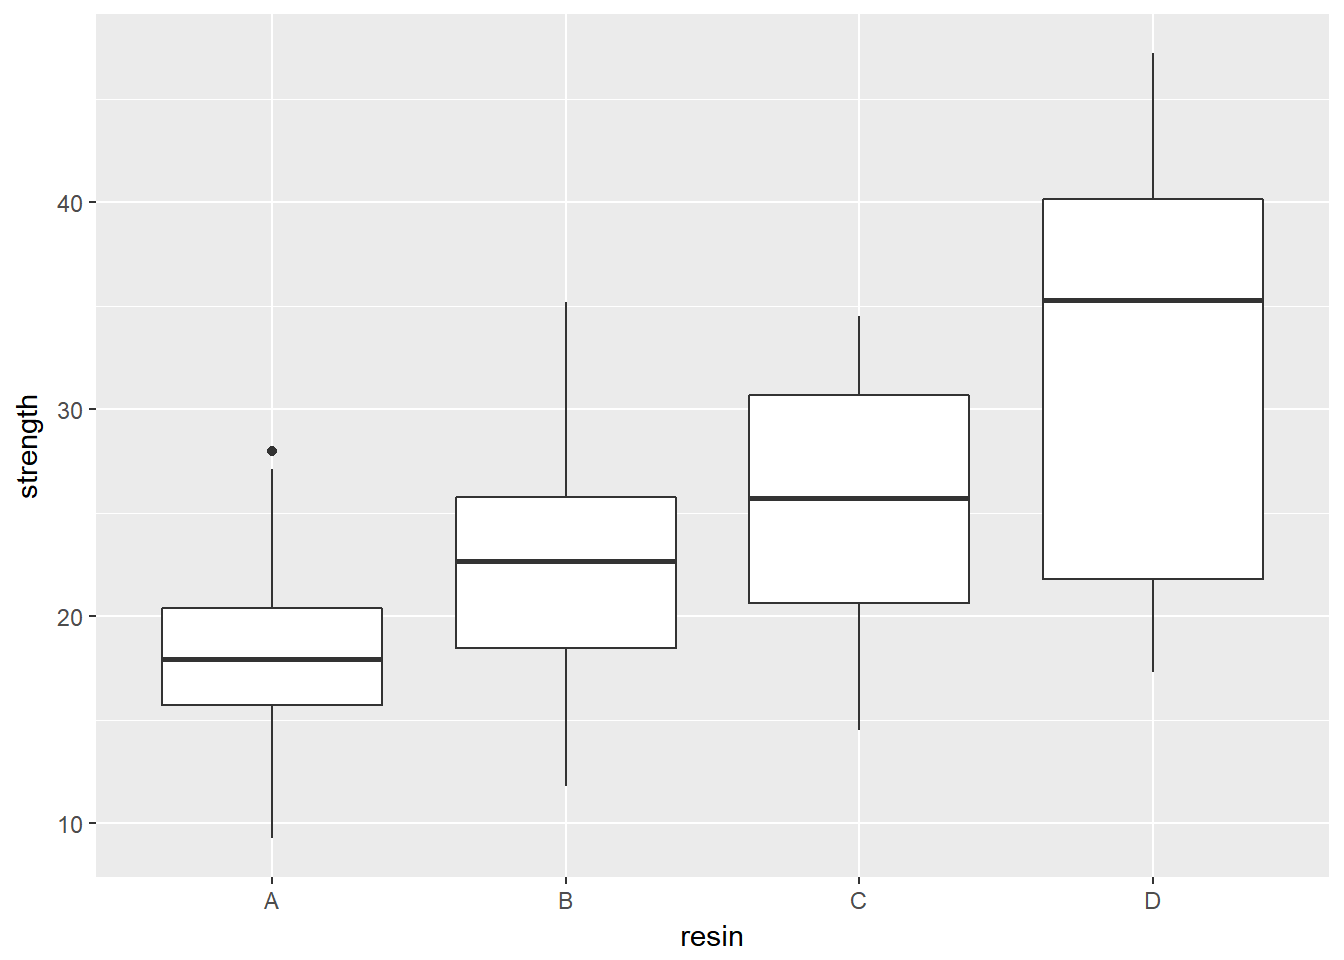
\includegraphics{bookdown-demo_files/figure-latex/c3_oneway_bonding_resin_boxplot-1.pdf}

Another good plot for this purpose is a ridgeline plot.

\begin{Shaded}
\begin{Highlighting}[]
\KeywordTok{ggplot}\NormalTok{(bonding, }\KeywordTok{aes}\NormalTok{(}\DataTypeTok{x =}\NormalTok{ strength, }\DataTypeTok{y =}\NormalTok{ resin, }\DataTypeTok{fill =}\NormalTok{ resin)) }\OperatorTok{+}
\StringTok{    }\KeywordTok{geom_density_ridges2}\NormalTok{() }\OperatorTok{+}
\StringTok{    }\KeywordTok{guides}\NormalTok{(}\DataTypeTok{fill =} \OtherTok{FALSE}\NormalTok{)}
\end{Highlighting}
\end{Shaded}

\begin{verbatim}
Picking joint bandwidth of 3.09
\end{verbatim}

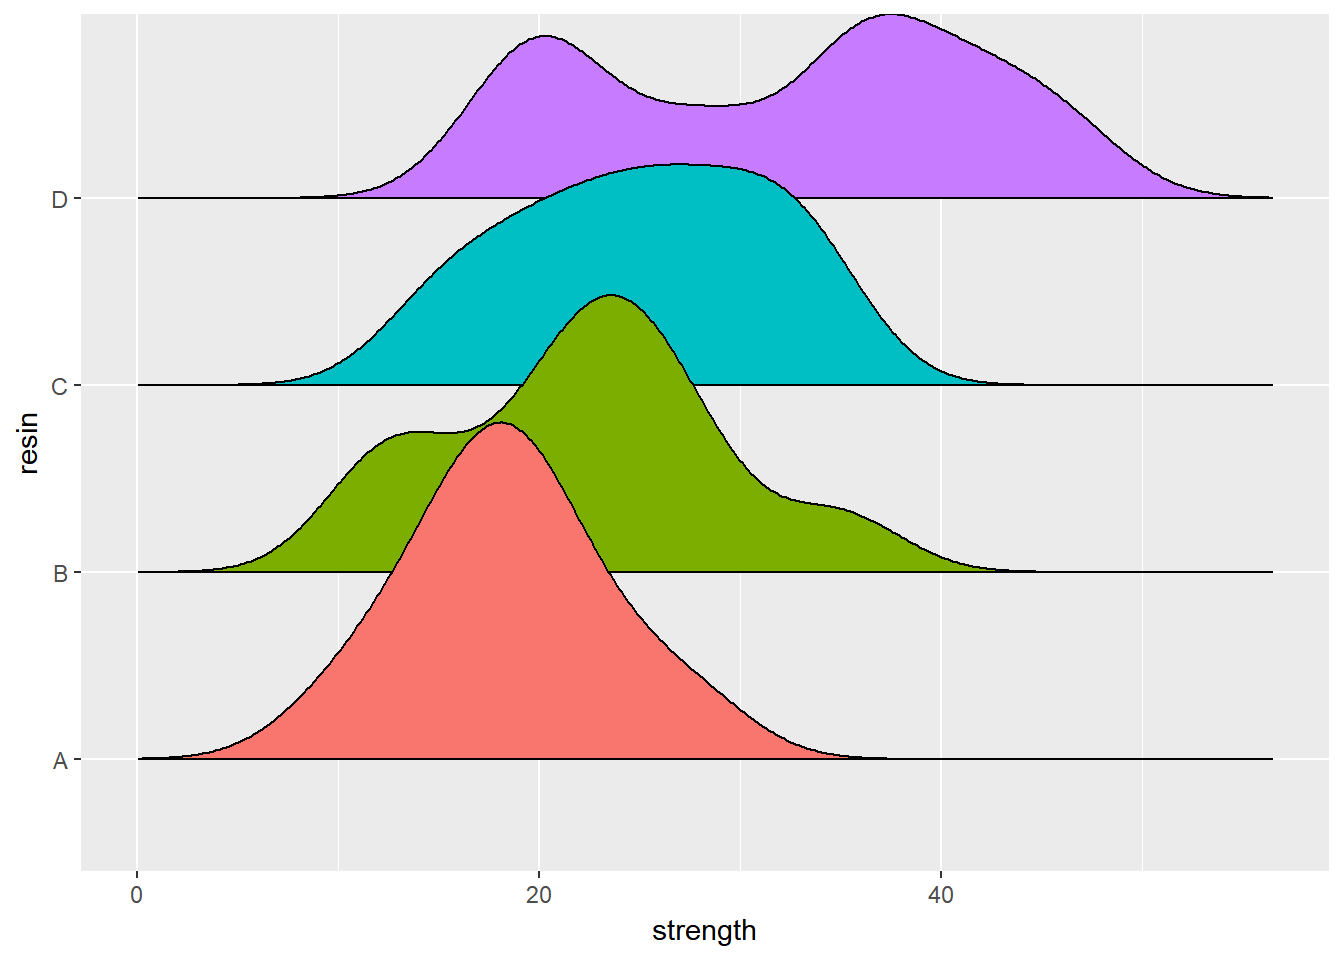
\includegraphics{bookdown-demo_files/figure-latex/c3_oneway_bonding_resin_ridgelineplot-1.pdf}

\subsection{Table of Summary
Statistics}\label{table-of-summary-statistics}

With the small size of this experiment (\emph{n} = 20 for each
\texttt{resin} type), graphical summaries may not perform as well as
they often do. We'll also produce a quick table of summary statistics
for \texttt{strength} within each \texttt{resin} type, with the
\texttt{skim()} function.

\begin{Shaded}
\begin{Highlighting}[]
\NormalTok{bonding }\OperatorTok\StringTok{ }\KeywordTok{group_by}\NormalTok{(resin) }\OperatorTok\StringTok{ }\KeywordTok{skim}\NormalTok{(strength)}
\end{Highlighting}
\end{Shaded}

\begin{verbatim}
Skim summary statistics
 n obs: 80 
 n variables: 4 
 group variables: resin 

Variable type: numeric 
 resin variable missing complete  n  mean   sd   p0   p25 median   p75
     A strength       0       20 20 18.41 4.81  9.3 15.73  17.95 20.4 
     B strength       0       20 20 22.23 6.75 11.8 18.45  22.7  25.75
     C strength       0       20 20 25.16 6.33 14.5 20.65  25.7  30.7 
     D strength       0       20 20 32.08 9.74 17.3 21.82  35.3  40.15
 p100
 28  
 35.2
 34.5
 47.2
\end{verbatim}

Since the means and medians within each group are fairly close, and the
distributions (with the possible exception of \texttt{resin} D) are
reasonably well approximated by the Normal, I'll fit an ANOVA
model\footnote{If the data weren't approximately Normally distributed,
  we might instead consider a rank-based alternative to ANOVA, like the
  Kruskal-Wallis test.}.

\begin{Shaded}
\begin{Highlighting}[]
\KeywordTok{anova}\NormalTok{(}\KeywordTok{lm}\NormalTok{(strength }\OperatorTok{~}\StringTok{ }\NormalTok{resin, }\DataTypeTok{data =}\NormalTok{ bonding))}
\end{Highlighting}
\end{Shaded}

\begin{verbatim}
Analysis of Variance Table

Response: strength
          Df Sum Sq Mean Sq F value   Pr(>F)    
resin      3 1999.7  666.57  13.107 5.52e-07 ***
Residuals 76 3865.2   50.86                     
---
Signif. codes:  0 '***' 0.001 '**' 0.01 '*' 0.05 '.' 0.1 ' ' 1
\end{verbatim}

It appears that the \texttt{resin} types have a significant association
with mean \texttt{strength} of the bonds. Can we identify which
\texttt{resin} types have generally higher or lower \texttt{strength}?

\begin{Shaded}
\begin{Highlighting}[]
\KeywordTok{TukeyHSD}\NormalTok{(}\KeywordTok{aov}\NormalTok{(}\KeywordTok{lm}\NormalTok{(strength }\OperatorTok{~}\StringTok{ }\NormalTok{resin, }\DataTypeTok{data =}\NormalTok{ bonding)))}
\end{Highlighting}
\end{Shaded}

\begin{verbatim}
  Tukey multiple comparisons of means
    95% family-wise confidence level

Fit: aov(formula = lm(strength ~ resin, data = bonding))

$resin
      diff        lwr       upr     p adj
B-A  3.815 -2.1088676  9.738868 0.3351635
C-A  6.740  0.8161324 12.663868 0.0193344
D-A 13.660  7.7361324 19.583868 0.0000003
C-B  2.925 -2.9988676  8.848868 0.5676635
D-B  9.845  3.9211324 15.768868 0.0002276
D-C  6.920  0.9961324 12.843868 0.0154615
\end{verbatim}

Based on these confidence intervals (which have a family-wise 95\%
confidence level), we see that D is associated with significantly larger
mean \texttt{strength} than A or B or C, and that C is also associated
with significantly larger mean \texttt{strength} than A. This may be
easier to see in a plot of these confidence intervals.

\begin{Shaded}
\begin{Highlighting}[]
\KeywordTok{plot}\NormalTok{(}\KeywordTok{TukeyHSD}\NormalTok{(}\KeywordTok{aov}\NormalTok{(}\KeywordTok{lm}\NormalTok{(strength }\OperatorTok{~}\StringTok{ }\NormalTok{resin, }\DataTypeTok{data =}\NormalTok{ bonding))))}
\end{Highlighting}
\end{Shaded}

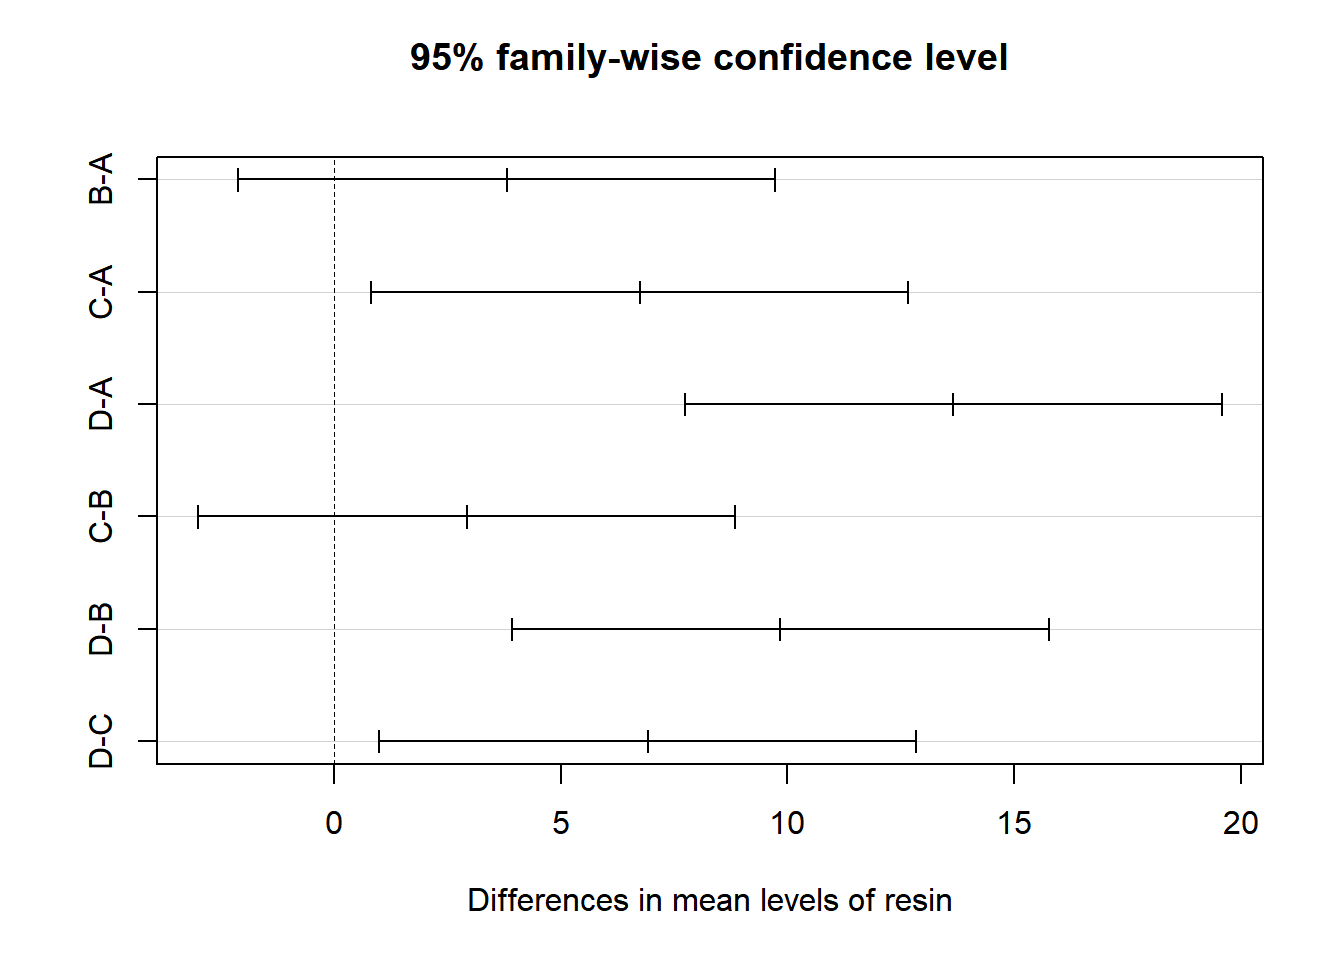
\includegraphics{bookdown-demo_files/figure-latex/unnamed-chunk-19-1.pdf}

\section{A Two-Way ANOVA: Looking at Two
Factors}\label{a-two-way-anova-looking-at-two-factors}

Now, we'll now add consideration of the \texttt{light} source into our
study. We can look at the distribution of the \texttt{strength} values
at the combinations of both \texttt{light} and \texttt{resin}, with a
plot like this one\ldots{}

\begin{Shaded}
\begin{Highlighting}[]
\KeywordTok{ggplot}\NormalTok{(bonding, }\KeywordTok{aes}\NormalTok{(}\DataTypeTok{x =}\NormalTok{ resin, }\DataTypeTok{y =}\NormalTok{ strength, }\DataTypeTok{color =}\NormalTok{ light)) }\OperatorTok{+}
\StringTok{    }\KeywordTok{geom_point}\NormalTok{(}\DataTypeTok{size =} \DecValTok{2}\NormalTok{, }\DataTypeTok{alpha =} \FloatTok{0.5}\NormalTok{) }\OperatorTok{+}
\StringTok{    }\KeywordTok{facet_wrap}\NormalTok{(}\OperatorTok{~}\StringTok{ }\NormalTok{light) }\OperatorTok{+}
\StringTok{    }\KeywordTok{guides}\NormalTok{(}\DataTypeTok{color =} \OtherTok{FALSE}\NormalTok{) }\OperatorTok{+}
\StringTok{    }\KeywordTok{scale_color_manual}\NormalTok{(}\DataTypeTok{values =} \KeywordTok{c}\NormalTok{(}\StringTok{"purple"}\NormalTok{, }\StringTok{"darkorange"}\NormalTok{)) }\OperatorTok{+}
\StringTok{    }\KeywordTok{theme_bw}\NormalTok{() }
\end{Highlighting}
\end{Shaded}

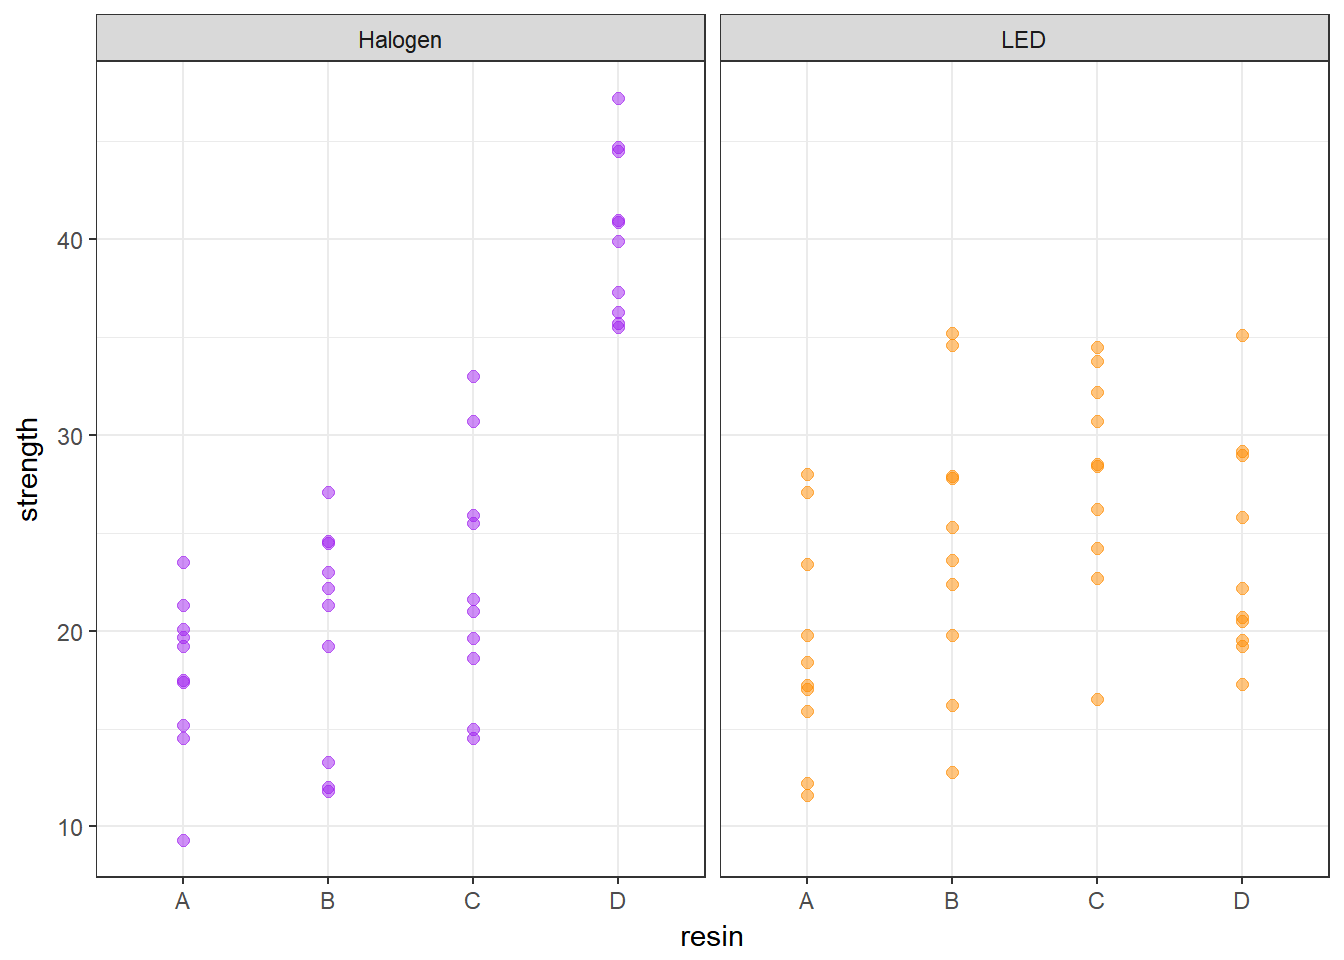
\includegraphics{bookdown-demo_files/figure-latex/c3_bonding_points_plot-1.pdf}

\section{A Means Plot (with standard deviations) to check for
interaction}\label{a-means-plot-with-standard-deviations-to-check-for-interaction}

Sometimes, we'll instead look at a plot simply of the means (and, often,
the standard deviations) of \texttt{strength} at each combination of
\texttt{light} and \texttt{resin}. We'll start by building up a data set
with the summaries we want to plot.

\begin{Shaded}
\begin{Highlighting}[]
\NormalTok{bond.sum <-}\StringTok{ }\NormalTok{bonding }\OperatorTok\StringTok{ }
\StringTok{    }\KeywordTok{group_by}\NormalTok{(resin, light) }\OperatorTok
\StringTok{    }\KeywordTok{summarize}\NormalTok{(}\DataTypeTok{mean.str =} \KeywordTok{mean}\NormalTok{(strength), }\DataTypeTok{sd.str =} \KeywordTok{sd}\NormalTok{(strength))}

\NormalTok{bond.sum}
\end{Highlighting}
\end{Shaded}

\begin{verbatim}
# A tibble: 8 x 4
# Groups:   resin [?]
  resin light   mean.str sd.str
  <fct> <fct>      <dbl>  <dbl>
1 A     Halogen     17.8   4.02
2 A     LED         19.1   5.63
3 B     Halogen     19.9   5.62
4 B     LED         24.6   7.25
5 C     Halogen     22.5   6.19
6 C     LED         27.8   5.56
7 D     Halogen     40.3   4.15
8 D     LED         23.8   5.70
\end{verbatim}

Now, we'll use this new data set to plot the means and standard
deviations of \texttt{strength} at each combination of \texttt{resin}
and \texttt{light}.

\begin{Shaded}
\begin{Highlighting}[]
\NormalTok{## The error bars will overlap unless we adjust the position.}
\NormalTok{pd <-}\StringTok{ }\KeywordTok{position_dodge}\NormalTok{(}\FloatTok{0.2}\NormalTok{) }\CommentTok{# move them .1 to the left and right}

\KeywordTok{ggplot}\NormalTok{(bond.sum, }\KeywordTok{aes}\NormalTok{(}\DataTypeTok{x =}\NormalTok{ resin, }\DataTypeTok{y =}\NormalTok{ mean.str, }\DataTypeTok{col =}\NormalTok{ light)) }\OperatorTok{+}
\StringTok{    }\KeywordTok{geom_errorbar}\NormalTok{(}\KeywordTok{aes}\NormalTok{(}\DataTypeTok{ymin =}\NormalTok{ mean.str }\OperatorTok{-}\StringTok{ }\NormalTok{sd.str, }
                      \DataTypeTok{ymax =}\NormalTok{ mean.str }\OperatorTok{+}\StringTok{ }\NormalTok{sd.str),}
                  \DataTypeTok{width =} \FloatTok{0.2}\NormalTok{, }\DataTypeTok{position =}\NormalTok{ pd) }\OperatorTok{+}
\StringTok{    }\KeywordTok{geom_point}\NormalTok{(}\DataTypeTok{size =} \DecValTok{2}\NormalTok{, }\DataTypeTok{position =}\NormalTok{ pd) }\OperatorTok{+}\StringTok{ }
\StringTok{    }\KeywordTok{geom_line}\NormalTok{(}\KeywordTok{aes}\NormalTok{(}\DataTypeTok{group =}\NormalTok{ light), }\DataTypeTok{position =}\NormalTok{ pd) }\OperatorTok{+}
\StringTok{    }\KeywordTok{scale_color_manual}\NormalTok{(}\DataTypeTok{values =} \KeywordTok{c}\NormalTok{(}\StringTok{"purple"}\NormalTok{, }\StringTok{"darkorange"}\NormalTok{)) }\OperatorTok{+}
\StringTok{    }\KeywordTok{theme_bw}\NormalTok{() }\OperatorTok{+}
\StringTok{    }\KeywordTok{labs}\NormalTok{(}\DataTypeTok{y =} \StringTok{"Bonding Strength (MPa)"}\NormalTok{, }\DataTypeTok{x =} \StringTok{"Resin Type"}\NormalTok{,}
         \DataTypeTok{title =} \StringTok{"Observed Means (+/- SD) of Bonding Strength"}\NormalTok{)}
\end{Highlighting}
\end{Shaded}

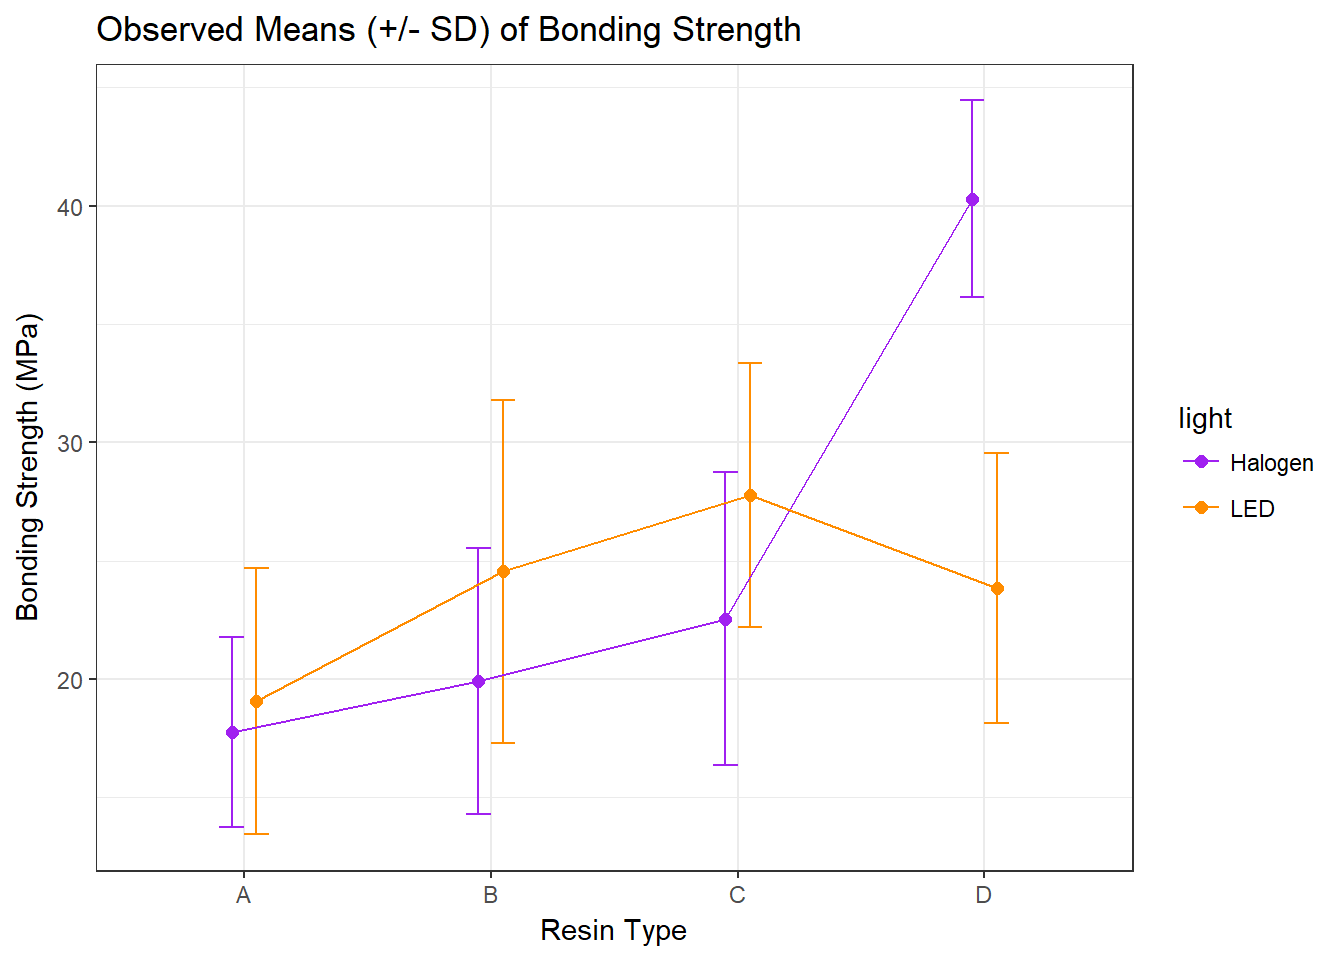
\includegraphics{bookdown-demo_files/figure-latex/c3_ggplot_means_plot_bonding-1.pdf}

Is there evidence of a meaningful interaction between the resin type and
the \texttt{light} source on the bonding strength in this plot?

\begin{itemize}
\tightlist
\item
  Sure. A meaningful interaction just means that the strength associated
  with different \texttt{resin} types depends on the \texttt{light}
  source.

  \begin{itemize}
  \tightlist
  \item
    With LED \texttt{light}, it appears that \texttt{resin} C leads to
    the strongest bonding strength.
  \item
    With Halogen \texttt{light}, though, it seems that \texttt{resin} D
    is substantially stronger.
  \end{itemize}
\item
  Note that the lines we see here connecting the \texttt{light} sources
  aren't in parallel (as they would be if we had zero interaction
  between \texttt{resin} and \texttt{light}), but rather, they cross.
\end{itemize}

\subsection{\texorpdfstring{Skimming the data after grouping by
\texttt{resin} and
\texttt{light}}{Skimming the data after grouping by resin and light}}\label{skimming-the-data-after-grouping-by-resin-and-light}

We might want to look at a numerical summary of the \texttt{strengths}
within these groups, too.

\begin{Shaded}
\begin{Highlighting}[]
\NormalTok{bonding }\OperatorTok
\StringTok{    }\KeywordTok{group_by}\NormalTok{(resin, light) }\OperatorTok
\StringTok{    }\KeywordTok{skim}\NormalTok{(strength) }
\end{Highlighting}
\end{Shaded}

\begin{verbatim}
Skim summary statistics
 n obs: 80 
 n variables: 4 
 group variables: resin, light 

Variable type: numeric 
 resin   light variable missing complete  n  mean   sd   p0   p25 median
     A Halogen strength       0       10 10 17.77 4.02  9.3 15.75  18.35
     A     LED strength       0       10 10 19.06 5.63 11.6 16.18  17.8 
     B Halogen strength       0       10 10 19.9  5.62 11.8 14.78  21.75
     B     LED strength       0       10 10 24.56 7.25 12.8 20.45  24.45
     C Halogen strength       0       10 10 22.54 6.19 14.5 18.85  21.3 
     C     LED strength       0       10 10 27.77 5.56 16.5 24.7   28.45
     D Halogen strength       0       10 10 40.3  4.15 35.5 36.55  40.4 
     D     LED strength       0       10 10 23.85 5.7  17.3 19.75  21.45
   p75 p100
 20    23.5
 22.5  28  
 24.12 27.1
 27.87 35.2
 25.8  33  
 31.83 34.5
 43.62 47.2
 28.2  35.1
\end{verbatim}

\section{Fitting the Two-Way ANOVA model with
Interaction}\label{fitting-the-two-way-anova-model-with-interaction}

\begin{Shaded}
\begin{Highlighting}[]
\NormalTok{c3_m1 <-}\StringTok{ }\KeywordTok{lm}\NormalTok{(strength }\OperatorTok{~}\StringTok{ }\NormalTok{resin }\OperatorTok{*}\StringTok{ }\NormalTok{light, }\DataTypeTok{data =}\NormalTok{ bonding)}

\KeywordTok{summary}\NormalTok{(c3_m1)}
\end{Highlighting}
\end{Shaded}

\begin{verbatim}

Call:
lm(formula = strength ~ resin * light, data = bonding)

Residuals:
    Min      1Q  Median      3Q     Max 
-11.760  -3.663  -0.320   3.697  11.250 

Coefficients:
                Estimate Std. Error t value Pr(>|t|)    
(Intercept)       17.770      1.771  10.033 2.57e-15 ***
resinB             2.130      2.505   0.850   0.3979    
resinC             4.770      2.505   1.904   0.0609 .  
resinD            22.530      2.505   8.995 2.13e-13 ***
lightLED           1.290      2.505   0.515   0.6081    
resinB:lightLED    3.370      3.542   0.951   0.3446    
resinC:lightLED    3.940      3.542   1.112   0.2697    
resinD:lightLED  -17.740      3.542  -5.008 3.78e-06 ***
---
Signif. codes:  0 '***' 0.001 '**' 0.01 '*' 0.05 '.' 0.1 ' ' 1

Residual standard error: 5.601 on 72 degrees of freedom
Multiple R-squared:  0.6149,    Adjusted R-squared:  0.5775 
F-statistic: 16.42 on 7 and 72 DF,  p-value: 9.801e-13
\end{verbatim}

\subsection{The ANOVA table for our
model}\label{the-anova-table-for-our-model}

In a two-way ANOVA model, we begin by assessing the interaction term. If
it's important, then our best model is the model including the
interaction. If it's not important, we will often move on to consider a
new model, fit without an interaction.

The ANOVA table is especially helpful in this case, because it lets us
look specifically at the interaction effect.

\begin{Shaded}
\begin{Highlighting}[]
\KeywordTok{anova}\NormalTok{(c3_m1)}
\end{Highlighting}
\end{Shaded}

\begin{verbatim}
Analysis of Variance Table

Response: strength
            Df  Sum Sq Mean Sq F value    Pr(>F)    
resin        3 1999.72  666.57 21.2499 5.792e-10 ***
light        1   34.72   34.72  1.1067    0.2963    
resin:light  3 1571.96  523.99 16.7043 2.457e-08 ***
Residuals   72 2258.52   31.37                      
---
Signif. codes:  0 '***' 0.001 '**' 0.01 '*' 0.05 '.' 0.1 ' ' 1
\end{verbatim}

\subsection{Is the interaction
important?}\label{is-the-interaction-important}

In this case, the interaction:

\begin{itemize}
\tightlist
\item
  is evident in the means plot, and
\item
  is highly statistically significant, and
\item
  accounts for a sizeable fraction (27\%) of the overall variation
\end{itemize}

\[ 
\eta^2_{interaction} = \frac{\mbox{SS(resin:light)}}{SS(Total)}
= \frac{1571.96}{1999.72 + 34.72 + 1571.96 + 2258.52} = 0.268
\]

If the interaction were \emph{either} large or significant we would be
inclined to keep it in the model. In this case, it's both, so there's no
real reason to remove it.

\subsection{Interpreting the
Interaction}\label{interpreting-the-interaction}

Recall the model equation, which is:

\begin{Shaded}
\begin{Highlighting}[]
\NormalTok{c3_m1}
\end{Highlighting}
\end{Shaded}

\begin{verbatim}

Call:
lm(formula = strength ~ resin * light, data = bonding)

Coefficients:
    (Intercept)           resinB           resinC           resinD  
          17.77             2.13             4.77            22.53  
       lightLED  resinB:lightLED  resinC:lightLED  resinD:lightLED  
           1.29             3.37             3.94           -17.74  
\end{verbatim}

so we have:

\[
strength = 17.77 + 2.13 resinB + 4.77 resinC + 22.53 resinD \\
+ 1.29 lightLED + 3.37 resinB*lightLED \\
+ 3.94 resinC*lightLED - 17.74 resinD*lightLED
\]

So, if \texttt{light} = Halogen, our equation is:

\[
strength = 17.77 + 2.13 resinB + 4.77 resinC + 22.53 resinD 
\]

And if \texttt{light} = LED, our equation is:

\[
strength = 19.06 + 5.50 resinB + 8.71 resinC + 4.79 resinD 
\]

Note that both the intercept and the slopes change as a result of the
interaction. The model yields a different prediction for every possible
combination of a \texttt{resin} type and a \texttt{light} source.

\section{\texorpdfstring{Comparing Individual Combinations of
\texttt{resin} and
\texttt{light}}{Comparing Individual Combinations of resin and light}}\label{comparing-individual-combinations-of-resin-and-light}

To make comparisons between individual combinations of a \texttt{resin}
type and a \texttt{light} source, using something like Tukey's HSD
approach for multiple comparisons, we first refit the model using the
\texttt{aov} structure, rather than \texttt{lm}.

\begin{Shaded}
\begin{Highlighting}[]
\NormalTok{c3m1_aov <-}\StringTok{ }\KeywordTok{aov}\NormalTok{(strength }\OperatorTok{~}\StringTok{ }\NormalTok{resin }\OperatorTok{*}\StringTok{ }\NormalTok{light, }\DataTypeTok{data =}\NormalTok{ bonding)}

\KeywordTok{summary}\NormalTok{(c3m1_aov)}
\end{Highlighting}
\end{Shaded}

\begin{verbatim}
            Df Sum Sq Mean Sq F value   Pr(>F)    
resin        3 1999.7   666.6  21.250 5.79e-10 ***
light        1   34.7    34.7   1.107    0.296    
resin:light  3 1572.0   524.0  16.704 2.46e-08 ***
Residuals   72 2258.5    31.4                     
---
Signif. codes:  0 '***' 0.001 '**' 0.01 '*' 0.05 '.' 0.1 ' ' 1
\end{verbatim}

And now, we can obtain Tukey HSD comparisons (which will maintain an
overall 95\% family-wise confidence level) across the \texttt{resin}
types, the \texttt{light} sources, and the combinations, with the
TukeyHSD command. This approach is only completely appropriate if these
comparisons are pre-planned, and if the design is balanced (as this is,
with the same sample size for each combination of a \texttt{light}
source and \texttt{resin} type.)

\begin{Shaded}
\begin{Highlighting}[]
\KeywordTok{TukeyHSD}\NormalTok{(c3m1_aov)}
\end{Highlighting}
\end{Shaded}

\begin{verbatim}
  Tukey multiple comparisons of means
    95% family-wise confidence level

Fit: aov(formula = strength ~ resin * light, data = bonding)

$resin
      diff       lwr       upr     p adj
B-A  3.815 -0.843129  8.473129 0.1461960
C-A  6.740  2.081871 11.398129 0.0016436
D-A 13.660  9.001871 18.318129 0.0000000
C-B  2.925 -1.733129  7.583129 0.3568373
D-B  9.845  5.186871 14.503129 0.0000026
D-C  6.920  2.261871 11.578129 0.0011731

$light
               diff       lwr      upr     p adj
LED-Halogen -1.3175 -3.814042 1.179042 0.2963128

$`resin:light`
                      diff          lwr        upr     p adj
B:Halogen-A:Halogen   2.13  -5.68928258   9.949283 0.9893515
C:Halogen-A:Halogen   4.77  -3.04928258  12.589283 0.5525230
D:Halogen-A:Halogen  22.53  14.71071742  30.349283 0.0000000
A:LED-A:Halogen       1.29  -6.52928258   9.109283 0.9995485
B:LED-A:Halogen       6.79  -1.02928258  14.609283 0.1361092
C:LED-A:Halogen      10.00   2.18071742  17.819283 0.0037074
D:LED-A:Halogen       6.08  -1.73928258  13.899283 0.2443200
C:Halogen-B:Halogen   2.64  -5.17928258  10.459283 0.9640100
D:Halogen-B:Halogen  20.40  12.58071742  28.219283 0.0000000
A:LED-B:Halogen      -0.84  -8.65928258   6.979283 0.9999747
B:LED-B:Halogen       4.66  -3.15928258  12.479283 0.5818695
C:LED-B:Halogen       7.87   0.05071742  15.689283 0.0473914
D:LED-B:Halogen       3.95  -3.86928258  11.769283 0.7621860
D:Halogen-C:Halogen  17.76   9.94071742  25.579283 0.0000000
A:LED-C:Halogen      -3.48 -11.29928258   4.339283 0.8591455
B:LED-C:Halogen       2.02  -5.79928258   9.839283 0.9922412
C:LED-C:Halogen       5.23  -2.58928258  13.049283 0.4323859
D:LED-C:Halogen       1.31  -6.50928258   9.129283 0.9995004
A:LED-D:Halogen     -21.24 -29.05928258 -13.420717 0.0000000
B:LED-D:Halogen     -15.74 -23.55928258  -7.920717 0.0000006
C:LED-D:Halogen     -12.53 -20.34928258  -4.710717 0.0001014
D:LED-D:Halogen     -16.45 -24.26928258  -8.630717 0.0000002
B:LED-A:LED           5.50  -2.31928258  13.319283 0.3665620
C:LED-A:LED           8.71   0.89071742  16.529283 0.0185285
D:LED-A:LED           4.79  -3.02928258  12.609283 0.5471915
C:LED-B:LED           3.21  -4.60928258  11.029283 0.9027236
D:LED-B:LED          -0.71  -8.52928258   7.109283 0.9999920
D:LED-C:LED          -3.92 -11.73928258   3.899283 0.7690762
\end{verbatim}

One conclusion from this is that the combination of D and Halogen is
significantly stronger than each of the other seven combinations.

\section{\texorpdfstring{The \texttt{bonding} model without
Interaction}{The bonding model without Interaction}}\label{the-bonding-model-without-interaction}

It seems incorrect in this situation to fit a model without the
interaction term, but we'll do so just so you can see what's involved.

\begin{Shaded}
\begin{Highlighting}[]
\NormalTok{c3_m2 <-}\StringTok{ }\KeywordTok{lm}\NormalTok{(strength }\OperatorTok{~}\StringTok{ }\NormalTok{resin }\OperatorTok{+}\StringTok{ }\NormalTok{light, }\DataTypeTok{data =}\NormalTok{ bonding)}

\KeywordTok{summary}\NormalTok{(c3_m2)}
\end{Highlighting}
\end{Shaded}

\begin{verbatim}

Call:
lm(formula = strength ~ resin + light, data = bonding)

Residuals:
     Min       1Q   Median       3Q      Max 
-14.1163  -4.9531   0.1187   4.4613  14.4663 

Coefficients:
            Estimate Std. Error t value Pr(>|t|)    
(Intercept)   19.074      1.787  10.676  < 2e-16 ***
resinB         3.815      2.260   1.688  0.09555 .  
resinC         6.740      2.260   2.982  0.00386 ** 
resinD        13.660      2.260   6.044 5.39e-08 ***
lightLED      -1.317      1.598  -0.824  0.41229    
---
Signif. codes:  0 '***' 0.001 '**' 0.01 '*' 0.05 '.' 0.1 ' ' 1

Residual standard error: 7.147 on 75 degrees of freedom
Multiple R-squared:  0.3469,    Adjusted R-squared:  0.312 
F-statistic: 9.958 on 4 and 75 DF,  p-value: 1.616e-06
\end{verbatim}

In the no-interaction model, if \texttt{light} = Halogen, our equation
is:

\[
strength = 19.07 + 3.82 resinB + 6.74 resinC + 13.66 resinD
\]

And if \texttt{light} = LED, our equation is:

\[
strength = 17.75 + 3.82 resinB + 6.74 resinC + 13.66 resinD
\]

So, in the no-interaction model, only the intercept changes.

\begin{Shaded}
\begin{Highlighting}[]
\KeywordTok{anova}\NormalTok{(c3_m2)}
\end{Highlighting}
\end{Shaded}

\begin{verbatim}
Analysis of Variance Table

Response: strength
          Df Sum Sq Mean Sq F value    Pr(>F)    
resin      3 1999.7  666.57 13.0514 6.036e-07 ***
light      1   34.7   34.72  0.6797    0.4123    
Residuals 75 3830.5   51.07                      
---
Signif. codes:  0 '***' 0.001 '**' 0.01 '*' 0.05 '.' 0.1 ' ' 1
\end{verbatim}

And, it appears, if we ignore the interaction, then \texttt{resin} type
has a significant impact on \texttt{strength} but \texttt{light} source
doesn't. This is clearer when we look at boxplots of the separated
\texttt{light} and \texttt{resin} groups.

\begin{Shaded}
\begin{Highlighting}[]
\NormalTok{p1 <-}\StringTok{ }\KeywordTok{ggplot}\NormalTok{(bonding, }\KeywordTok{aes}\NormalTok{(}\DataTypeTok{x =}\NormalTok{ light, }\DataTypeTok{y =}\NormalTok{ strength)) }\OperatorTok{+}\StringTok{ }
\StringTok{    }\KeywordTok{geom_boxplot}\NormalTok{()}
\NormalTok{p2 <-}\StringTok{ }\KeywordTok{ggplot}\NormalTok{(bonding, }\KeywordTok{aes}\NormalTok{(}\DataTypeTok{x =}\NormalTok{ resin, }\DataTypeTok{y =}\NormalTok{ strength)) }\OperatorTok{+}
\StringTok{    }\KeywordTok{geom_boxplot}\NormalTok{()}

\NormalTok{gridExtra}\OperatorTok{::}\KeywordTok{grid.arrange}\NormalTok{(p1, p2, }\DataTypeTok{nrow =} \DecValTok{1}\NormalTok{)}
\end{Highlighting}
\end{Shaded}

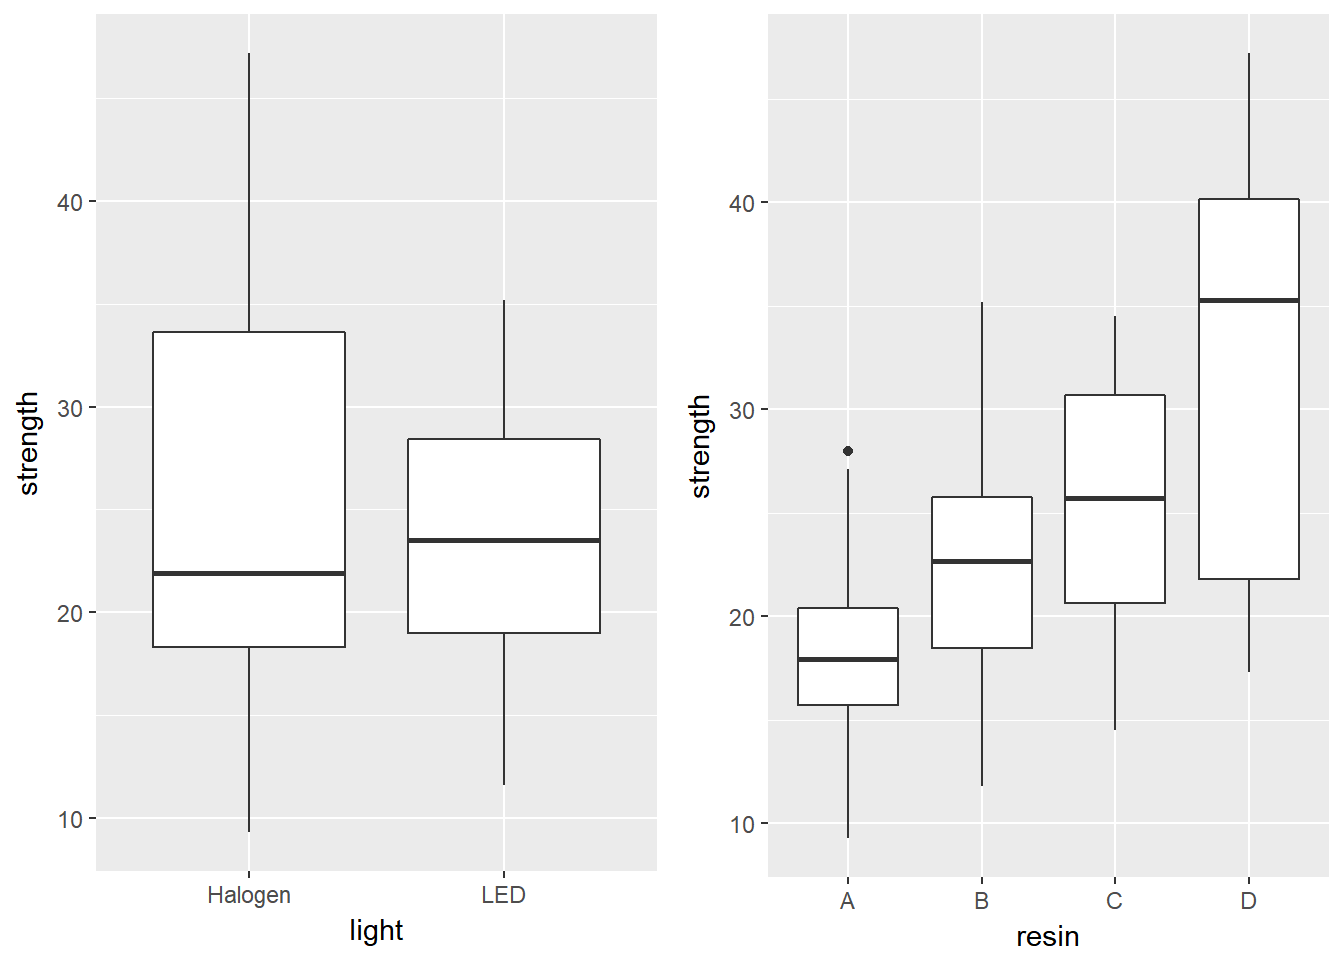
\includegraphics{bookdown-demo_files/figure-latex/boxplots_c3_bonding_without_interaction-1.pdf}

\section{\texorpdfstring{\texttt{cortisol}: A Hypothetical Clinical
Trial}{cortisol: A Hypothetical Clinical Trial}}\label{cortisol-a-hypothetical-clinical-trial}

156 adults who complained of problems with a high-stress lifestyle were
enrolled in a hypothetical clinical trial of the effectiveness of a
behavioral intervention designed to help reduce stress levels, as
measured by salivary cortisol.

The subjects were randomly assigned to one of three intervention groups
(usual care, low dose, and high dose.) The ``low dose'' subjects
received a one-week intervention with a follow-up at week 5. The ``high
dose'' subjects received a more intensive three-week intervention, with
follow up at week 5.

Since cortisol levels rise and fall with circadian rhythms, the cortisol
measurements were taken just after rising for all subjects. These
measurements were taken at baseline, and again at five weeks. The
difference (baseline - week 5) in cortisol level (in micrograms / l)
serves as the primary outcome.

\subsection{\texorpdfstring{Codebook and Raw Data for
\texttt{cortisol}}{Codebook and Raw Data for cortisol}}\label{codebook-and-raw-data-for-cortisol}

The data are gathered in the \texttt{cortisol} data set. Included are:

\begin{longtable}[]{@{}rl@{}}
\toprule
Variable & Description\tabularnewline
\midrule
\endhead
\texttt{subject} & subject identification code\tabularnewline
\texttt{interv} & intervention group (UC = usual care, Low,
High)\tabularnewline
\texttt{waist} & waist circumference at baseline (in
inches)\tabularnewline
\texttt{sex} & male or female\tabularnewline
\texttt{cort.1} & salivary cortisol level (microg/l) week
1\tabularnewline
\texttt{cort.5} & salivary cortisol level (microg/l) week
5\tabularnewline
\bottomrule
\end{longtable}

\begin{Shaded}
\begin{Highlighting}[]
\NormalTok{cortisol}
\end{Highlighting}
\end{Shaded}

\begin{verbatim}
# A tibble: 156 x 6
   subject interv waist sex   cort.1 cort.5
     <int> <fct>  <dbl> <fct>  <dbl>  <dbl>
 1    1001 UC      48.3 M      13.4   13.3 
 2    1002 Low     58.3 M      17.8   16.6 
 3    1003 High    43.0 M      14.4   12.7 
 4    1004 Low     44.9 M       9.00   9.80
 5    1005 High    46.1 M      14.2   14.2 
 6    1006 UC      41.3 M      14.8   15.1 
 7    1007 Low     51.0 F      13.7   16.0 
 8    1008 UC      42.0 F      17.3   18.7 
 9    1009 Low     24.7 F      15.3   15.8 
10    1010 Low     59.4 M      12.4   11.7 
# ... with 146 more rows
\end{verbatim}

\section{Creating a factor combining sex and
waist}\label{creating-a-factor-combining-sex-and-waist}

Next, we'll put the \texttt{waist} and \texttt{sex} data in the
\texttt{cortisol} example together. We want to build a second
categorical variable (called \texttt{fat\_est}) combining this
information, to indicate ``healthy'' vs. ``unhealthy'' levels of fat
around the waist.

\begin{itemize}
\tightlist
\item
  Male subjects whose waist circumference is 40 inches or more, and
\item
  Female subjects whose waist circumference is 35 inches or more, will
  fall in the ``unhealthy'' group.
\end{itemize}

\begin{Shaded}
\begin{Highlighting}[]
\NormalTok{cortisol <-}\StringTok{ }\NormalTok{cortisol }\OperatorTok
\StringTok{    }\KeywordTok{mutate}\NormalTok{(}
        \DataTypeTok{fat_est =} \KeywordTok{factor}\NormalTok{(}\KeywordTok{case_when}\NormalTok{(}
\NormalTok{            sex }\OperatorTok{==}\StringTok{ "M"} \OperatorTok{&}\StringTok{ }\NormalTok{waist }\OperatorTok{>=}\StringTok{ }\DecValTok{40} \OperatorTok{~}\StringTok{ "unhealthy"}\NormalTok{,}
\NormalTok{            sex }\OperatorTok{==}\StringTok{ "F"} \OperatorTok{&}\StringTok{ }\NormalTok{waist }\OperatorTok{>=}\StringTok{ }\DecValTok{35} \OperatorTok{~}\StringTok{ "unhealthy"}\NormalTok{,}
            \OtherTok{TRUE}                     \OperatorTok{~}\StringTok{ "healthy"}\NormalTok{)),}
        \DataTypeTok{cort_diff =}\NormalTok{ cort.}\DecValTok{1} \OperatorTok{-}\StringTok{ }\NormalTok{cort.}\DecValTok{5}\NormalTok{)}

\KeywordTok{summary}\NormalTok{(cortisol)}
\end{Highlighting}
\end{Shaded}

\begin{verbatim}
    subject      interv       waist       sex        cort.1      
 Min.   :1001   High:53   Min.   :20.80   F:83   Min.   : 6.000  
 1st Qu.:1040   Low :52   1st Qu.:33.27   M:73   1st Qu.: 9.675  
 Median :1078   UC  :51   Median :40.35          Median :12.400  
 Mean   :1078             Mean   :40.42          Mean   :12.686  
 3rd Qu.:1117             3rd Qu.:47.77          3rd Qu.:16.025  
 Max.   :1156             Max.   :59.90          Max.   :19.000  
     cort.5          fat_est      cort_diff      
 Min.   : 4.2   healthy  : 56   Min.   :-2.3000  
 1st Qu.: 9.6   unhealthy:100   1st Qu.:-0.5000  
 Median :12.6                   Median : 0.2000  
 Mean   :12.4                   Mean   : 0.2821  
 3rd Qu.:15.7                   3rd Qu.: 1.2000  
 Max.   :19.7                   Max.   : 2.0000  
\end{verbatim}

\section{\texorpdfstring{A Means Plot for the \texttt{cortisol} trial
(with standard
errors)}{A Means Plot for the cortisol trial (with standard errors)}}\label{a-means-plot-for-the-cortisol-trial-with-standard-errors}

Again, we'll start by building up a data set with the summaries we want
to plot.

\begin{Shaded}
\begin{Highlighting}[]
\NormalTok{cort.sum <-}\StringTok{ }\NormalTok{cortisol }\OperatorTok\StringTok{ }
\StringTok{    }\KeywordTok{group_by}\NormalTok{(interv, fat_est) }\OperatorTok
\StringTok{    }\KeywordTok{summarize}\NormalTok{(}\DataTypeTok{mean.cort =} \KeywordTok{mean}\NormalTok{(cort_diff), }
              \DataTypeTok{se.cort =} \KeywordTok{sd}\NormalTok{(cort_diff)}\OperatorTok{/}\KeywordTok{sqrt}\NormalTok{(}\KeywordTok{n}\NormalTok{()))}

\NormalTok{cort.sum}
\end{Highlighting}
\end{Shaded}

\begin{verbatim}
# A tibble: 6 x 4
# Groups:   interv [?]
  interv fat_est   mean.cort se.cort
  <fct>  <fct>         <dbl>   <dbl>
1 High   healthy       0.695   0.217
2 High   unhealthy     0.352   0.150
3 Low    healthy       0.500   0.182
4 Low    unhealthy     0.327   0.190
5 UC     healthy       0.347   0.225
6 UC     unhealthy    -0.226   0.155
\end{verbatim}

Now, we'll use this new data set to plot the means and standard errors.

\begin{Shaded}
\begin{Highlighting}[]
\NormalTok{## The error bars will overlap unless we adjust the position.}
\NormalTok{pd <-}\StringTok{ }\KeywordTok{position_dodge}\NormalTok{(}\FloatTok{0.2}\NormalTok{) }\CommentTok{# move them .1 to the left and right}

\KeywordTok{ggplot}\NormalTok{(cort.sum, }\KeywordTok{aes}\NormalTok{(}\DataTypeTok{x =}\NormalTok{ interv, }\DataTypeTok{y =}\NormalTok{ mean.cort, }\DataTypeTok{col =}\NormalTok{ fat_est)) }\OperatorTok{+}
\StringTok{    }\KeywordTok{geom_errorbar}\NormalTok{(}\KeywordTok{aes}\NormalTok{(}\DataTypeTok{ymin =}\NormalTok{ mean.cort }\OperatorTok{-}\StringTok{ }\NormalTok{se.cort, }
                      \DataTypeTok{ymax =}\NormalTok{ mean.cort }\OperatorTok{+}\StringTok{ }\NormalTok{se.cort),}
                  \DataTypeTok{width =} \FloatTok{0.2}\NormalTok{, }\DataTypeTok{position =}\NormalTok{ pd) }\OperatorTok{+}
\StringTok{    }\KeywordTok{geom_point}\NormalTok{(}\DataTypeTok{size =} \DecValTok{2}\NormalTok{, }\DataTypeTok{position =}\NormalTok{ pd) }\OperatorTok{+}\StringTok{ }
\StringTok{    }\KeywordTok{geom_line}\NormalTok{(}\KeywordTok{aes}\NormalTok{(}\DataTypeTok{group =}\NormalTok{ fat_est), }\DataTypeTok{position =}\NormalTok{ pd) }\OperatorTok{+}
\StringTok{    }\KeywordTok{scale_color_manual}\NormalTok{(}\DataTypeTok{values =} \KeywordTok{c}\NormalTok{(}\StringTok{"royalblue"}\NormalTok{, }\StringTok{"darkred"}\NormalTok{)) }\OperatorTok{+}
\StringTok{    }\KeywordTok{theme_bw}\NormalTok{() }\OperatorTok{+}
\StringTok{    }\KeywordTok{labs}\NormalTok{(}\DataTypeTok{y =} \StringTok{"Salivary Cortisol Level"}\NormalTok{, }\DataTypeTok{x =} \StringTok{"Intervention Group"}\NormalTok{,}
         \DataTypeTok{title =} \StringTok{"Observed Means (+/- SE) of Salivary Cortisol"}\NormalTok{)}
\end{Highlighting}
\end{Shaded}

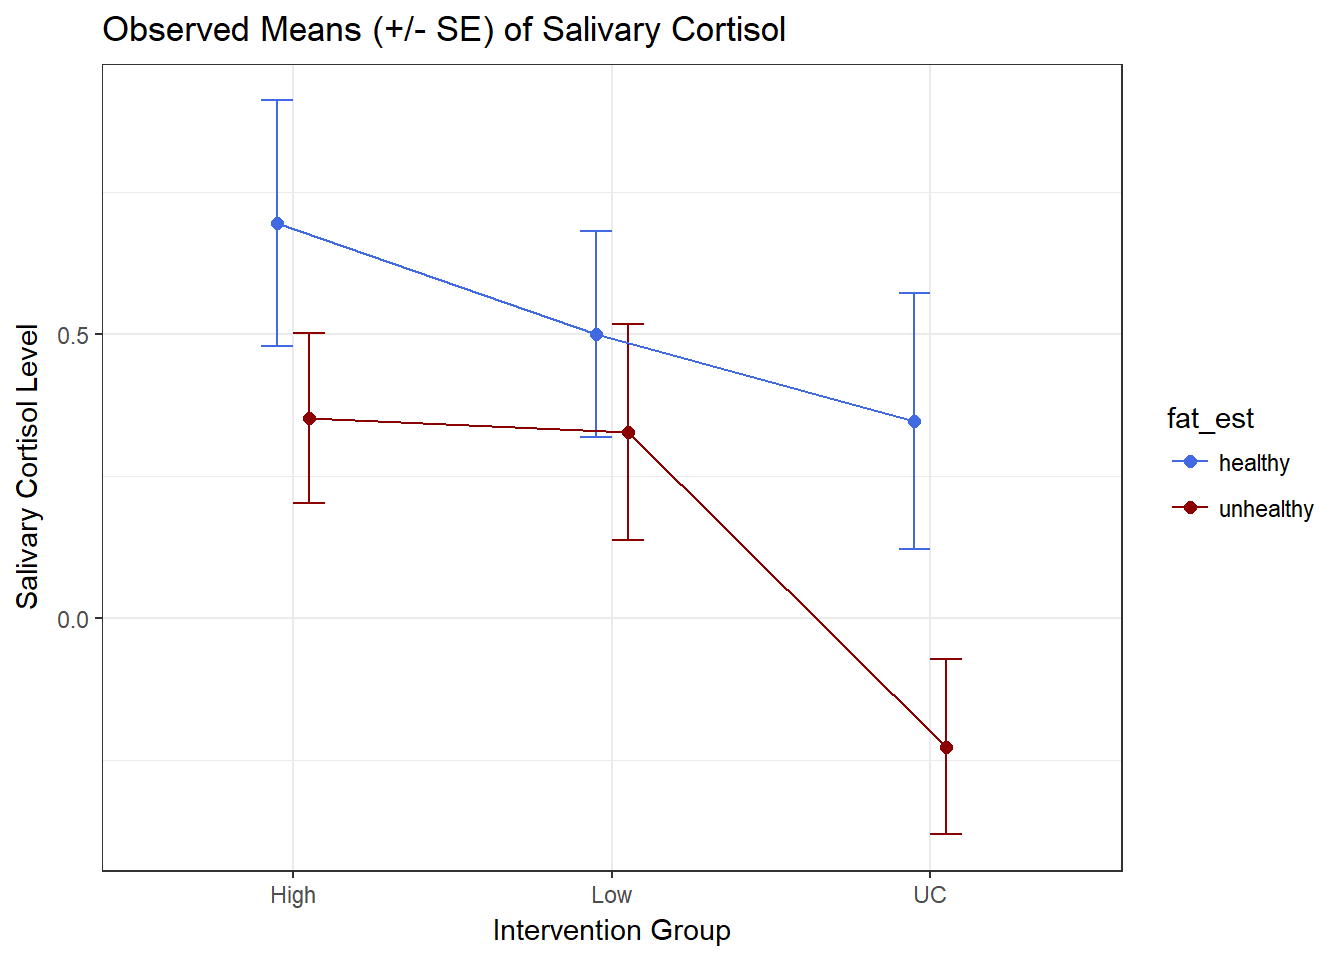
\includegraphics{bookdown-demo_files/figure-latex/c3_ggplot_means_plot_cortisol-1.pdf}

\section{\texorpdfstring{A Two-Way ANOVA model for \texttt{cortisol}
with
Interaction}{A Two-Way ANOVA model for cortisol with Interaction}}\label{a-two-way-anova-model-for-cortisol-with-interaction}

\begin{Shaded}
\begin{Highlighting}[]
\NormalTok{c3_m3 <-}\StringTok{ }\KeywordTok{lm}\NormalTok{(cort_diff }\OperatorTok{~}\StringTok{ }\NormalTok{interv }\OperatorTok{*}\StringTok{ }\NormalTok{fat_est, }\DataTypeTok{data =}\NormalTok{ cortisol)}

\KeywordTok{anova}\NormalTok{(c3_m3)}
\end{Highlighting}
\end{Shaded}

\begin{verbatim}
Analysis of Variance Table

Response: cort_diff
                Df  Sum Sq Mean Sq F value  Pr(>F)  
interv           2   7.847  3.9235  4.4698 0.01301 *
fat_est          1   4.614  4.6139  5.2564 0.02326 *
interv:fat_est   2   0.943  0.4715  0.5371 0.58554  
Residuals      150 131.666  0.8778                  
---
Signif. codes:  0 '***' 0.001 '**' 0.01 '*' 0.05 '.' 0.1 ' ' 1
\end{verbatim}

Does it seem like we need the interaction term in this case?

\begin{Shaded}
\begin{Highlighting}[]
\KeywordTok{summary}\NormalTok{(c3_m3)}
\end{Highlighting}
\end{Shaded}

\begin{verbatim}

Call:
lm(formula = cort_diff ~ interv * fat_est, data = cortisol)

Residuals:
     Min       1Q   Median       3Q      Max 
-2.62727 -0.75702  0.08636  0.84848  2.12647 

Coefficients:
                           Estimate Std. Error t value Pr(>|t|)   
(Intercept)                  0.6950     0.2095   3.317  0.00114 **
intervLow                   -0.1950     0.3001  -0.650  0.51689   
intervUC                    -0.3479     0.3091  -1.126  0.26206   
fat_estunhealthy            -0.3435     0.2655  -1.294  0.19774   
intervLow:fat_estunhealthy   0.1708     0.3785   0.451  0.65256   
intervUC:fat_estunhealthy   -0.2300     0.3846  -0.598  0.55068   
---
Signif. codes:  0 '***' 0.001 '**' 0.01 '*' 0.05 '.' 0.1 ' ' 1

Residual standard error: 0.9369 on 150 degrees of freedom
Multiple R-squared:  0.0924,    Adjusted R-squared:  0.06214 
F-statistic: 3.054 on 5 and 150 DF,  p-value: 0.01179
\end{verbatim}

How do you reconcile the apparent difference in significance levels
between this regression summary and the ANOVA table above?

\section{\texorpdfstring{A Two-Way ANOVA model for \texttt{cortisol}
without
Interaction}{A Two-Way ANOVA model for cortisol without Interaction}}\label{a-two-way-anova-model-for-cortisol-without-interaction}

\subsection{The Graph}\label{the-graph}

\begin{Shaded}
\begin{Highlighting}[]
\NormalTok{p1 <-}\StringTok{ }\KeywordTok{ggplot}\NormalTok{(cortisol, }\KeywordTok{aes}\NormalTok{(}\DataTypeTok{x =}\NormalTok{ interv, }\DataTypeTok{y =}\NormalTok{ cort_diff)) }\OperatorTok{+}\StringTok{ }
\StringTok{    }\KeywordTok{geom_boxplot}\NormalTok{()}
\NormalTok{p2 <-}\StringTok{ }\KeywordTok{ggplot}\NormalTok{(cortisol, }\KeywordTok{aes}\NormalTok{(}\DataTypeTok{x =}\NormalTok{ fat_est, }\DataTypeTok{y =}\NormalTok{ cort_diff)) }\OperatorTok{+}
\StringTok{    }\KeywordTok{geom_boxplot}\NormalTok{()}

\NormalTok{gridExtra}\OperatorTok{::}\KeywordTok{grid.arrange}\NormalTok{(p1, p2, }\DataTypeTok{nrow =} \DecValTok{1}\NormalTok{)}
\end{Highlighting}
\end{Shaded}

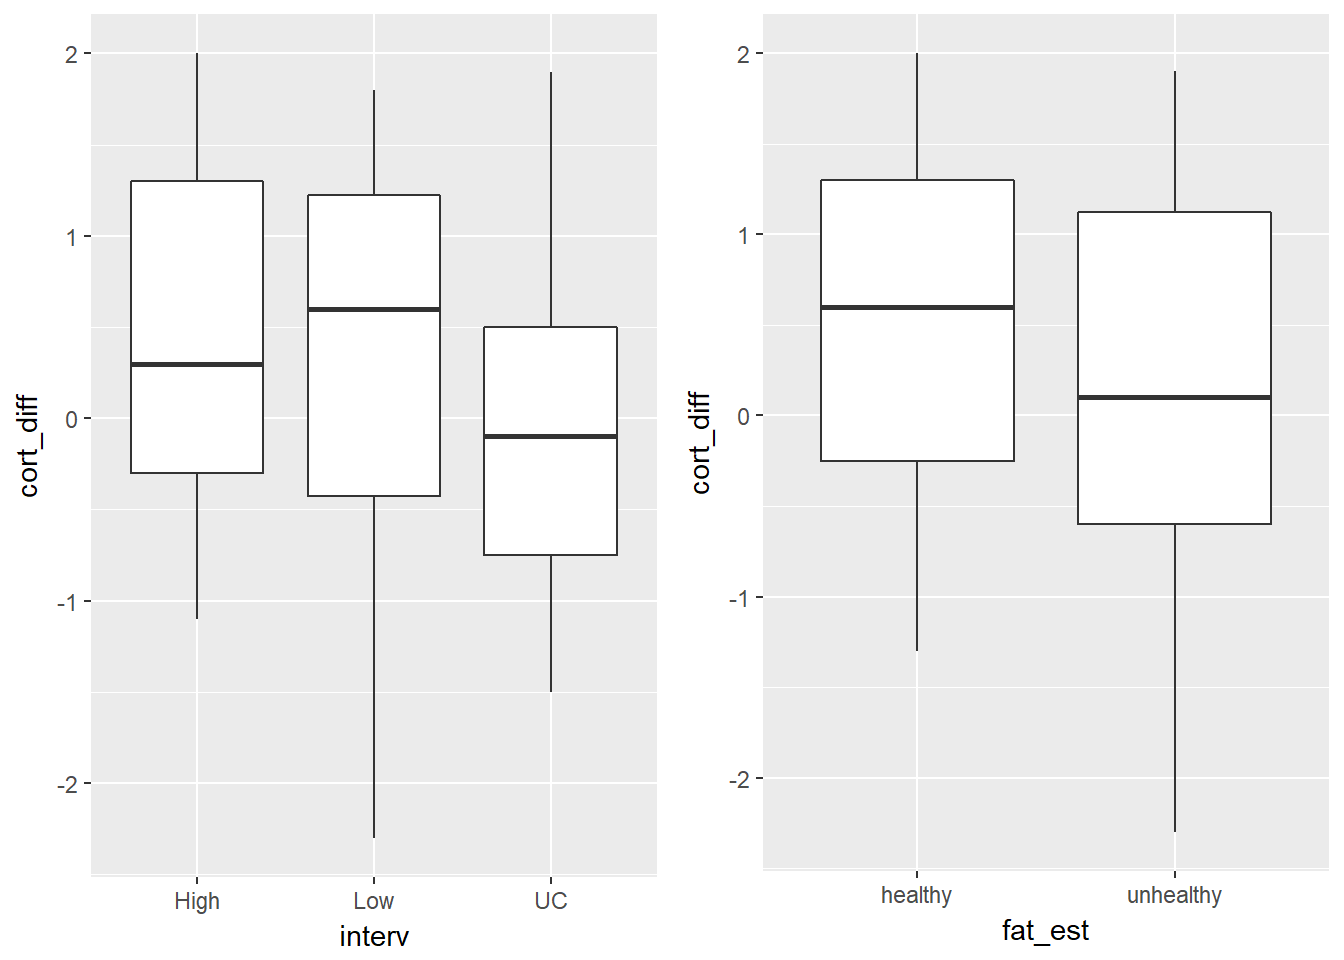
\includegraphics{bookdown-demo_files/figure-latex/boxplots_c3_cortisol_without_interaction-1.pdf}

\subsection{The ANOVA Model}\label{the-anova-model}

\begin{Shaded}
\begin{Highlighting}[]
\NormalTok{c3_m4 <-}\StringTok{ }\KeywordTok{lm}\NormalTok{(cort_diff }\OperatorTok{~}\StringTok{ }\NormalTok{interv }\OperatorTok{+}\StringTok{ }\NormalTok{fat_est, }\DataTypeTok{data =}\NormalTok{ cortisol)}

\KeywordTok{anova}\NormalTok{(c3_m4)}
\end{Highlighting}
\end{Shaded}

\begin{verbatim}
Analysis of Variance Table

Response: cort_diff
           Df  Sum Sq Mean Sq F value  Pr(>F)  
interv      2   7.847  3.9235  4.4972 0.01266 *
fat_est     1   4.614  4.6139  5.2886 0.02283 *
Residuals 152 132.609  0.8724                  
---
Signif. codes:  0 '***' 0.001 '**' 0.01 '*' 0.05 '.' 0.1 ' ' 1
\end{verbatim}

How do these results compare to those we saw in the model with
interaction?

\subsection{The Regression Summary}\label{the-regression-summary}

\begin{Shaded}
\begin{Highlighting}[]
\KeywordTok{summary}\NormalTok{(c3_m4)}
\end{Highlighting}
\end{Shaded}

\begin{verbatim}

Call:
lm(formula = cort_diff ~ interv + fat_est, data = cortisol)

Residuals:
     Min       1Q   Median       3Q      Max 
-2.55929 -0.74527  0.05457  0.86456  2.05489 

Coefficients:
                 Estimate Std. Error t value Pr(>|t|)    
(Intercept)       0.70452    0.16093   4.378 2.22e-05 ***
intervLow        -0.08645    0.18232  -0.474  0.63606    
intervUC         -0.50063    0.18334  -2.731  0.00707 ** 
fat_estunhealthy -0.35878    0.15601  -2.300  0.02283 *  
---
Signif. codes:  0 '***' 0.001 '**' 0.01 '*' 0.05 '.' 0.1 ' ' 1

Residual standard error: 0.934 on 152 degrees of freedom
Multiple R-squared:  0.0859,    Adjusted R-squared:  0.06785 
F-statistic: 4.761 on 3 and 152 DF,  p-value: 0.00335
\end{verbatim}

\subsection{Tukey HSD Comparisons}\label{tukey-hsd-comparisons}

Without the interaction term, we can make direct comparisons between
levels of the intervention, and between levels of the \texttt{fat\_est}
variable. This is probably best done here in a Tukey HSD comparison.

\begin{Shaded}
\begin{Highlighting}[]
\KeywordTok{TukeyHSD}\NormalTok{(}\KeywordTok{aov}\NormalTok{(cort_diff }\OperatorTok{~}\StringTok{ }\NormalTok{interv }\OperatorTok{+}\StringTok{ }\NormalTok{fat_est, }\DataTypeTok{data =}\NormalTok{ cortisol))}
\end{Highlighting}
\end{Shaded}

\begin{verbatim}
  Tukey multiple comparisons of means
    95% family-wise confidence level

Fit: aov(formula = cort_diff ~ interv + fat_est, data = cortisol)

$interv
                diff        lwr         upr     p adj
Low-High -0.09074746 -0.5222655  0.34077063 0.8724916
UC-High  -0.51642619 -0.9500745 -0.08277793 0.0150150
UC-Low   -0.42567873 -0.8613670  0.01000948 0.0570728

$fat_est
                        diff        lwr         upr     p adj
unhealthy-healthy -0.3582443 -0.6662455 -0.05024305 0.0229266
\end{verbatim}

What conclusions can we draw, at a 5\% significance level?

\chapter{Analysis of Covariance}\label{analysis-of-covariance}

\section{An Emphysema Study}\label{an-emphysema-study}

My source for this example is \citet{Riffenburgh2006}, section 18.4.
Serum theophylline levels (in mg/dl) were measured in 16 patients with
emphysema at baseline, then 5 days later (at the end of a course of
antibiotics) and then at 10 days after baseline. Clinicians anticipate
that the antibiotic will increase the theophylline level. The data are
stored in the \texttt{emphysema.csv} data file, and note that the age
for patient 5 is not available.

\subsection{Codebook}\label{codebook}

\begin{longtable}[]{@{}rl@{}}
\toprule
Variable & Description\tabularnewline
\midrule
\endhead
\texttt{patient} & ID code\tabularnewline
\texttt{age} & patient's age in years\tabularnewline
\texttt{sex} & patient's sex (F or M)\tabularnewline
\texttt{st\_base} & patient's serum theophylline at baseline
(mg/dl)\tabularnewline
\texttt{st\_day5} & patient's serum theophylline at day 5
(mg/dl)\tabularnewline
\texttt{st\_day10} & patient's serum theophylline at day 10
(mg/dl)\tabularnewline
\bottomrule
\end{longtable}

We're going to look at the change from baseline to day 5 as our outcome
of interest, since the clinical expectation is that the antibiotic
(azithromycin) will increase theophylline levels.

\begin{Shaded}
\begin{Highlighting}[]
\NormalTok{emphysema <-}\StringTok{ }\NormalTok{emphysema }\OperatorTok\StringTok{ }
\StringTok{    }\KeywordTok{mutate}\NormalTok{(}\DataTypeTok{st_delta =}\NormalTok{ st_day5 }\OperatorTok{-}\StringTok{ }\NormalTok{st_base)}

\NormalTok{emphysema}
\end{Highlighting}
\end{Shaded}

\begin{verbatim}
# A tibble: 16 x 7
   patient   age sex   st_base st_day5 st_day10 st_delta
     <int> <int> <fct>   <dbl>   <dbl>    <dbl>    <dbl>
 1       1    61 F       14.1     2.30    10.3   -11.8  
 2       2    70 F        7.20    5.40     7.30   -1.80 
 3       3    65 M       14.2    11.9     11.3    -2.30 
 4       4    65 M       10.3    10.7     13.8     0.400
 5       5    NA M        9.90   10.7     11.7     0.800
 6       6    76 M        5.20    6.80     4.20    1.60 
 7       7    72 M       10.4    14.6     14.1     4.20 
 8       8    69 F       10.5     7.20     5.40   -3.30 
 9       9    66 M        5.00    5.00     5.10    0.   
10      10    62 M        8.60    8.10     7.40   -0.500
11      11    65 F       16.6    14.9     13.0    -1.70 
12      12    71 M       16.4    18.6     17.1     2.20 
13      13    51 F       12.2    11.0     12.3    -1.20 
14      14    71 M        6.60    3.70     4.50   -2.90 
15      15    64 F       15.4    15.2     13.6    -0.200
16      16    50 M       10.2    10.8     11.2     0.600
\end{verbatim}

\section{\texorpdfstring{Does \texttt{sex} affect the mean change in
theophylline?}{Does sex affect the mean change in theophylline?}}\label{does-sex-affect-the-mean-change-in-theophylline}

\begin{Shaded}
\begin{Highlighting}[]
\NormalTok{emphysema }\OperatorTok\StringTok{ }\KeywordTok{skim}\NormalTok{(st_delta)}
\end{Highlighting}
\end{Shaded}

\begin{verbatim}
Skim summary statistics
 n obs: 16 
 n variables: 7 

Variable type: numeric 
 variable missing complete  n  mean   sd    p0   p25 median  p75 p100
 st_delta       0       16 16 -0.99 3.48 -11.8 -1.92  -0.35 0.65  4.2
\end{verbatim}

\begin{Shaded}
\begin{Highlighting}[]
\NormalTok{emphysema }\OperatorTok\StringTok{ }\KeywordTok{group_by}\NormalTok{(sex) }\OperatorTok\StringTok{ }\KeywordTok{skim}\NormalTok{(st_delta)}
\end{Highlighting}
\end{Shaded}

\begin{verbatim}
Skim summary statistics
 n obs: 16 
 n variables: 7 
 group variables: sex 

Variable type: numeric 
 sex variable missing complete  n  mean   sd    p0   p25 median   p75 p100
   F st_delta       0        6  6 -3.33 4.27 -11.8 -2.92  -1.75 -1.32 -0.2
   M st_delta       0       10 10  0.41 2.07  -2.9 -0.38   0.5   1.4   4.2
\end{verbatim}

Overall, the mean change in theophylline during the course of the
antibiotic is -0.99, but this is -3.33 for female patients and 0.41 for
male patients.

A one-way ANOVA model looks like this:

\begin{Shaded}
\begin{Highlighting}[]
\KeywordTok{anova}\NormalTok{(}\KeywordTok{lm}\NormalTok{(st_delta }\OperatorTok{~}\StringTok{ }\NormalTok{sex, }\DataTypeTok{data =}\NormalTok{ emphysema))}
\end{Highlighting}
\end{Shaded}

\begin{verbatim}
Analysis of Variance Table

Response: st_delta
          Df  Sum Sq Mean Sq F value  Pr(>F)  
sex        1  52.547  52.547  5.6789 0.03189 *
Residuals 14 129.542   9.253                  
---
Signif. codes:  0 '***' 0.001 '**' 0.01 '*' 0.05 '.' 0.1 ' ' 1
\end{verbatim}

The ANOVA F test finds a statistically significant difference between
the mean \texttt{st\_delta} among males and the mean \texttt{st\_delta}
among females. But is there more to the story?

\section{\texorpdfstring{Is there an association between \texttt{age}
and \texttt{sex} in this
study?}{Is there an association between age and sex in this study?}}\label{is-there-an-association-between-age-and-sex-in-this-study}

\begin{Shaded}
\begin{Highlighting}[]
\NormalTok{emphysema }\OperatorTok\StringTok{ }\KeywordTok{group_by}\NormalTok{(sex) }\OperatorTok\StringTok{ }\KeywordTok{skim}\NormalTok{(age)}
\end{Highlighting}
\end{Shaded}

\begin{verbatim}
Skim summary statistics
 n obs: 16 
 n variables: 7 
 group variables: sex 

Variable type: integer 
 sex variable missing complete  n  mean   sd p0   p25 median p75 p100
   F      age       0        6  6 63.33 6.89 51 61.75   64.5  68   70
   M      age       1        9 10 66.44 7.57 50 65      66    71   76
\end{verbatim}

But we note that the male patients are also older than the female
patients, on average (mean age for males is 66.4, for females 63.3)

\begin{itemize}
\tightlist
\item
  Does the fact that male patients are older affect change in
  theophylline level?
\item
  And how should we deal with the one missing \texttt{age} value (in a
  male patient)?
\end{itemize}

\section{\texorpdfstring{Adding a quantitative covariate, \texttt{age},
to the
model}{Adding a quantitative covariate, age, to the model}}\label{adding-a-quantitative-covariate-age-to-the-model}

We could fit an ANOVA model to predict \texttt{st\_delta} using
\texttt{sex} and \texttt{age} directly, but only if we categorized
\texttt{age} into two or more groups. Because \texttt{age} is not
categorical, we cannot include it in an ANOVA. But if age is an
influence, and we don't adjust for it, it may well bias the outcome of
our initial ANOVA. With a quantitative variable like \texttt{age}, we
will need a method called ANCOVA, for \textbf{analysis of covariance}.

\subsection{The ANCOVA model}\label{the-ancova-model}

ANCOVA in this case is just an ANOVA model with our outcome
(\texttt{st\_delta}) adjusted for a continuous covariate, called
\texttt{age}. For the moment, we'll ignore the one subject with missing
\texttt{age} and simply fit the regression model with \texttt{sex} and
\texttt{age}.

\begin{Shaded}
\begin{Highlighting}[]
\KeywordTok{summary}\NormalTok{(}\KeywordTok{lm}\NormalTok{(st_delta }\OperatorTok{~}\StringTok{ }\NormalTok{sex }\OperatorTok{+}\StringTok{ }\NormalTok{age, }\DataTypeTok{data =}\NormalTok{ emphysema))}
\end{Highlighting}
\end{Shaded}

\begin{verbatim}

Call:
lm(formula = st_delta ~ sex + age, data = emphysema)

Residuals:
    Min      1Q  Median      3Q     Max 
-8.3352 -0.4789  0.6948  1.5580  3.5202 

Coefficients:
            Estimate Std. Error t value Pr(>|t|)  
(Intercept) -6.90266    7.92948  -0.871   0.4011  
sexM         3.52466    1.75815   2.005   0.0681 .
age          0.05636    0.12343   0.457   0.6561  
---
Signif. codes:  0 '***' 0.001 '**' 0.01 '*' 0.05 '.' 0.1 ' ' 1

Residual standard error: 3.255 on 12 degrees of freedom
  (1 observation deleted due to missingness)
Multiple R-squared:  0.2882,    Adjusted R-squared:  0.1696 
F-statistic:  2.43 on 2 and 12 DF,  p-value: 0.13
\end{verbatim}

This model assumes that the slope of the regression line between
\texttt{st\_delta} and \texttt{age} is the same for both sexes.

Note that the model yields \texttt{st\_delta} = -6.9 + 3.52
(\texttt{sex} = male) + 0.056 \texttt{age}, or

\begin{itemize}
\tightlist
\item
  \texttt{st\_delta} = -6.9 + 0.056 \texttt{age} for female patients,
  and
\item
  \texttt{st\_delta} = (-6.9 + 3.52) + 0.056 \texttt{age} = -3.38 +
  0.056 \texttt{age} for male patients.
\end{itemize}

Note that we can test this assumption of equal slopes by fitting an
alternative model (with a product term between \texttt{sex} and
\texttt{age}) that doesn't require the assumption, and we'll do that
later.

\subsection{The ANCOVA Table}\label{the-ancova-table}

First, though, we'll look at the ANCOVA table.

\begin{Shaded}
\begin{Highlighting}[]
\KeywordTok{anova}\NormalTok{(}\KeywordTok{lm}\NormalTok{(st_delta }\OperatorTok{~}\StringTok{ }\NormalTok{sex }\OperatorTok{+}\StringTok{ }\NormalTok{age, }\DataTypeTok{data =}\NormalTok{ emphysema))}
\end{Highlighting}
\end{Shaded}

\begin{verbatim}
Analysis of Variance Table

Response: st_delta
          Df  Sum Sq Mean Sq F value  Pr(>F)  
sex        1  49.284  49.284  4.6507 0.05203 .
age        1   2.209   2.209  0.2085 0.65612  
Residuals 12 127.164  10.597                  
---
Signif. codes:  0 '***' 0.001 '**' 0.01 '*' 0.05 '.' 0.1 ' ' 1
\end{verbatim}

When we tested \texttt{sex} without accounting for \texttt{age}, we
found a \emph{p} value of 0.032, which is less than our usual cutpoint
of 0.05. But when we adjusted for \texttt{age}, we find that
\texttt{sex} loses significance, even though \texttt{age} is not a
significant influence on \texttt{st\_delta} by itself, according to the
ANCOVA table.

\section{Rerunning the ANCOVA model after simple
imputation}\label{rerunning-the-ancova-model-after-simple-imputation}

We could have \emph{imputed} the missing \texttt{age} value for patient
5, rather than just deleting that patient. Suppose we do the simplest
potentially reasonable thing to do: insert the mean \texttt{age} in
where the NA value currently exists.

\begin{Shaded}
\begin{Highlighting}[]
\NormalTok{emph_imp <-}\StringTok{ }\KeywordTok{replace_na}\NormalTok{(emphysema, }\KeywordTok{list}\NormalTok{(}\DataTypeTok{age =} \KeywordTok{mean}\NormalTok{(emphysema}\OperatorTok{$}\NormalTok{age, }\DataTypeTok{na.rm =} \OtherTok{TRUE}\NormalTok{)))}

\NormalTok{emph_imp}
\end{Highlighting}
\end{Shaded}

\begin{verbatim}
# A tibble: 16 x 7
   patient   age sex   st_base st_day5 st_day10 st_delta
     <int> <dbl> <fct>   <dbl>   <dbl>    <dbl>    <dbl>
 1       1  61.0 F       14.1     2.30    10.3   -11.8  
 2       2  70.0 F        7.20    5.40     7.30   -1.80 
 3       3  65.0 M       14.2    11.9     11.3    -2.30 
 4       4  65.0 M       10.3    10.7     13.8     0.400
 5       5  65.2 M        9.90   10.7     11.7     0.800
 6       6  76.0 M        5.20    6.80     4.20    1.60 
 7       7  72.0 M       10.4    14.6     14.1     4.20 
 8       8  69.0 F       10.5     7.20     5.40   -3.30 
 9       9  66.0 M        5.00    5.00     5.10    0.   
10      10  62.0 M        8.60    8.10     7.40   -0.500
11      11  65.0 F       16.6    14.9     13.0    -1.70 
12      12  71.0 M       16.4    18.6     17.1     2.20 
13      13  51.0 F       12.2    11.0     12.3    -1.20 
14      14  71.0 M        6.60    3.70     4.50   -2.90 
15      15  64.0 F       15.4    15.2     13.6    -0.200
16      16  50.0 M       10.2    10.8     11.2     0.600
\end{verbatim}

More on simple imputation and missing data is coming soon.

For now, we can rerun the ANCOVA model on this new data set, after
imputation\ldots{}

\begin{Shaded}
\begin{Highlighting}[]
\KeywordTok{anova}\NormalTok{(}\KeywordTok{lm}\NormalTok{(st_delta }\OperatorTok{~}\StringTok{ }\NormalTok{sex }\OperatorTok{+}\StringTok{ }\NormalTok{age, }\DataTypeTok{data =}\NormalTok{ emph_imp))}
\end{Highlighting}
\end{Shaded}

\begin{verbatim}
Analysis of Variance Table

Response: st_delta
          Df  Sum Sq Mean Sq F value  Pr(>F)  
sex        1  52.547  52.547  5.3623 0.03755 *
age        1   2.151   2.151  0.2195 0.64721  
Residuals 13 127.392   9.799                  
---
Signif. codes:  0 '***' 0.001 '**' 0.01 '*' 0.05 '.' 0.1 ' ' 1
\end{verbatim}

When we do this, we see that now the \texttt{sex} variable returns to a
\emph{p} value below 0.05. Our complete case analysis (which omitted
patient 5) gives us a different result than the ANCOVA based on the data
after mean imputation.

\section{Looking at a factor-covariate
interaction}\label{looking-at-a-factor-covariate-interaction}

Let's run a model including the interaction (product) term between
\texttt{age} and \texttt{sex}, which implies that the slope of
\texttt{age} on our outcome (\texttt{st\_delta}) depends on the
patient's sex. We'll use the imputed data again. Here is the new ANCOVA
table, which suggests that the interaction of \texttt{age} and
\texttt{sex} is small (because it accounts for only a small amount of
the total Sum of Squares) and not significant (p = 0.91).

\begin{Shaded}
\begin{Highlighting}[]
\KeywordTok{anova}\NormalTok{(}\KeywordTok{lm}\NormalTok{(st_delta }\OperatorTok{~}\StringTok{ }\NormalTok{sex }\OperatorTok{*}\StringTok{ }\NormalTok{age, }\DataTypeTok{data =}\NormalTok{ emph_imp))}
\end{Highlighting}
\end{Shaded}

\begin{verbatim}
Analysis of Variance Table

Response: st_delta
          Df  Sum Sq Mean Sq F value  Pr(>F)  
sex        1  52.547  52.547  4.9549 0.04594 *
age        1   2.151   2.151  0.2028 0.66051  
sex:age    1   0.130   0.130  0.0123 0.91355  
Residuals 12 127.261  10.605                  
---
Signif. codes:  0 '***' 0.001 '**' 0.01 '*' 0.05 '.' 0.1 ' ' 1
\end{verbatim}

Since the interaction term is neither substantial nor significant, we
probably don't need it here. But let's look at its interpretation
anyway, just to fix ideas. To do that, we'll need the coefficients from
the underlying regression model.

\begin{Shaded}
\begin{Highlighting}[]
\KeywordTok{tidy}\NormalTok{(}\KeywordTok{lm}\NormalTok{(st_delta }\OperatorTok{~}\StringTok{ }\NormalTok{sex }\OperatorTok{*}\StringTok{ }\NormalTok{age, }\DataTypeTok{data =}\NormalTok{ emph_imp))}
\end{Highlighting}
\end{Shaded}

\begin{verbatim}
         term    estimate  std.error  statistic   p.value
1 (Intercept) -5.64606742 13.4536974 -0.4196666 0.6821446
2        sexM  1.72031026 16.8389209  0.1021627 0.9203148
3         age  0.03651685  0.2113871  0.1727488 0.8657284
4    sexM:age  0.02885946  0.2603044  0.1108681 0.9135536
\end{verbatim}

Our ANCOVA model for \texttt{st\_delta} incorporating the \texttt{age} x
\texttt{sex} product term is -5.65 + 1.72 (sex = M) + 0.037 age + 0.029
(sex = M)(age). So that means:

\begin{itemize}
\tightlist
\item
  our model for females is \texttt{st\_delta} = -5.65 + 0.037
  \texttt{age}
\item
  our model for males is \texttt{st\_delta} = (-5.65 + 1.72) + (0.037 +
  0.029) \texttt{age}, or -3.93 + 0.066 \texttt{age}
\end{itemize}

but, again, our conclusion from the ANCOVA table is that this increase
in complexity (letting both the slope and intercept vary by
\texttt{sex}) doesn't add much in the way of predictive value for our
\texttt{st\_delta} outcome.

\section{Centering the Covariate to Facilitate ANCOVA
Interpretation}\label{centering-the-covariate-to-facilitate-ancova-interpretation}

When developing an ANCOVA model, we will often \textbf{center} or even
\textbf{center and rescale} the covariate to facilitate interpretation
of the product term. In this case, let's center \texttt{age} and rescale
it by dividing by two standard deviations.

\begin{Shaded}
\begin{Highlighting}[]
\NormalTok{emph_imp }\OperatorTok\StringTok{ }\KeywordTok{skim}\NormalTok{(age)}
\end{Highlighting}
\end{Shaded}

\begin{verbatim}
Skim summary statistics
 n obs: 16 
 n variables: 7 

Variable type: numeric 
 variable missing complete  n mean   sd p0  p25 median   p75 p100
      age       0       16 16 65.2 6.98 50 63.5   65.1 70.25   76
\end{verbatim}

Note that in our imputed data, the mean \texttt{age} is 65.2 and the
standard deviation of \texttt{age} is 7 years.

So we build the rescaled \texttt{age} variable that I'll call
\texttt{age\_z}, and then use it to refit our model.

\begin{Shaded}
\begin{Highlighting}[]
\NormalTok{emph_imp <-}\StringTok{ }\NormalTok{emph_imp }\OperatorTok
\StringTok{    }\KeywordTok{mutate}\NormalTok{(}\DataTypeTok{age_z =}\NormalTok{ (age }\OperatorTok{-}\StringTok{ }\KeywordTok{mean}\NormalTok{(age))}\OperatorTok{/}\StringTok{ }\NormalTok{(}\DecValTok{2} \OperatorTok{*}\StringTok{ }\KeywordTok{sd}\NormalTok{(age)))}

\KeywordTok{anova}\NormalTok{(}\KeywordTok{lm}\NormalTok{(st_delta }\OperatorTok{~}\StringTok{ }\NormalTok{sex }\OperatorTok{*}\StringTok{ }\NormalTok{age_z, }\DataTypeTok{data =}\NormalTok{ emph_imp))}
\end{Highlighting}
\end{Shaded}

\begin{verbatim}
Analysis of Variance Table

Response: st_delta
          Df  Sum Sq Mean Sq F value  Pr(>F)  
sex        1  52.547  52.547  4.9549 0.04594 *
age_z      1   2.151   2.151  0.2028 0.66051  
sex:age_z  1   0.130   0.130  0.0123 0.91355  
Residuals 12 127.261  10.605                  
---
Signif. codes:  0 '***' 0.001 '**' 0.01 '*' 0.05 '.' 0.1 ' ' 1
\end{verbatim}

\begin{Shaded}
\begin{Highlighting}[]
\KeywordTok{tidy}\NormalTok{(}\KeywordTok{lm}\NormalTok{(st_delta }\OperatorTok{~}\StringTok{ }\NormalTok{sex }\OperatorTok{*}\StringTok{ }\NormalTok{age_z, }\DataTypeTok{data =}\NormalTok{ emph_imp))}
\end{Highlighting}
\end{Shaded}

\begin{verbatim}
         term   estimate std.error  statistic    p.value
1 (Intercept) -3.2651685  1.386802 -2.3544587 0.03641637
2        sexM  3.6019471  1.735706  2.0752055 0.06013138
3       age_z  0.5096337  2.950144  0.1727488 0.86572835
4  sexM:age_z  0.4027661  3.632839  0.1108681 0.91355364
\end{verbatim}

Comparing the two models, we have:

\begin{itemize}
\tightlist
\item
  (unscaled): \texttt{st\_delta} = -5.65 + 1.72 (\texttt{sex} = M) +
  0.037 \texttt{age} + 0.029 (\texttt{sex} = M) x (\texttt{age})
\item
  (rescaled): \texttt{st\_delta} = -3.27 + 3.60 (\texttt{sex} = M) +
  0.510 rescaled \texttt{age\_z} + 0.402 (\texttt{sex} = M) x (rescaled
  \texttt{age\_z})
\end{itemize}

In essence, the rescaled model on \texttt{age\_z} is:

\begin{itemize}
\tightlist
\item
  \texttt{st\_delta} = -3.27 + 0.510 \texttt{age\_z} for female
  subjects, and
\item
  \texttt{st\_delta} = (-3.27 + 3.60) + (0.510 + 0.402) \texttt{age\_z}
  = 0.33 + 0.912 \texttt{age\_z} for male subjects
\end{itemize}

Interpreting the centered, rescaled model, we have:

\begin{itemize}
\tightlist
\item
  no change in the ANOVA results or R-squared or residual standard
  deviation compared to the uncentered, unscaled model, but
\item
  the intercept (-3.27) now represents the \texttt{st\_delta} for a
  female of average age,
\item
  the \texttt{sex} slope (3.60) represents the (male - female)
  difference in predicted \texttt{st\_delta} for a person of average
  age,
\item
  the \texttt{age\_z} slope (0.510) represents the difference in
  predicted \texttt{st\_delta} for a female one standard deviation older
  than the mean age as compared to a female one standard deviation
  younger than the mean age, and
\item
  the product term's slope (0.402) represents the male - female
  difference in the slope of \texttt{age\_z}, so that if you add the
  \texttt{age\_z} slope (0.510) and the interaction slope (0.402) you
  see the difference in predicted \texttt{st\_delta} for a male one
  standard deviation older than the mean age as compared to a male one
  standard deviation younger than the mean age.
\end{itemize}

\chapter{Missing Data Mechanisms and Single
Imputation}\label{missing-data-mechanisms-and-single-imputation}

Almost all serious statistical analyses have to deal with missing data.
Data values that are missing are indicated in R, and to R, by the symbol
\texttt{NA}.

\section{A Toy Example}\label{a-toy-example}

In the following tiny data set called \texttt{sbp\_example}, we have
four variables for a set of 15 subjects. In addition to a subject id, we
have:

\begin{itemize}
\tightlist
\item
  the treatment this subject received (A, B or C are the treatments),
\item
  an indicator (1 = yes, 0 = no) of whether the subject has diabetes,
\item
  the subject's systolic blood pressure at baseline
\item
  the subject's systolic blood pressure after the application of the
  treatment
\end{itemize}

\begin{Shaded}
\begin{Highlighting}[]
\CommentTok{# create some temporary variables}

\NormalTok{subject <-}\StringTok{ }\DecValTok{101}\OperatorTok{:}\DecValTok{115}
\NormalTok{x1 <-}\StringTok{ }\KeywordTok{c}\NormalTok{(}\StringTok{"A"}\NormalTok{, }\StringTok{"B"}\NormalTok{, }\StringTok{"C"}\NormalTok{, }\StringTok{"A"}\NormalTok{, }\StringTok{"C"}\NormalTok{, }\StringTok{"A"}\NormalTok{, }\StringTok{"A"}\NormalTok{, }\OtherTok{NA}\NormalTok{, }\StringTok{"B"}\NormalTok{, }\StringTok{"C"}\NormalTok{, }\StringTok{"A"}\NormalTok{, }\StringTok{"B"}\NormalTok{, }\StringTok{"C"}\NormalTok{, }\StringTok{"A"}\NormalTok{, }\StringTok{"B"}\NormalTok{)}
\NormalTok{x2 <-}\StringTok{ }\KeywordTok{c}\NormalTok{(}\DecValTok{1}\NormalTok{, }\DecValTok{0}\NormalTok{, }\DecValTok{0}\NormalTok{, }\DecValTok{1}\NormalTok{, }\OtherTok{NA}\NormalTok{, }\DecValTok{1}\NormalTok{, }\DecValTok{0}\NormalTok{, }\DecValTok{1}\NormalTok{, }\OtherTok{NA}\NormalTok{, }\DecValTok{1}\NormalTok{, }\DecValTok{0}\NormalTok{, }\DecValTok{0}\NormalTok{, }\DecValTok{1}\NormalTok{, }\DecValTok{1}\NormalTok{, }\OtherTok{NA}\NormalTok{)}
\NormalTok{x3 <-}\StringTok{ }\KeywordTok{c}\NormalTok{(}\DecValTok{120}\NormalTok{, }\DecValTok{145}\NormalTok{, }\DecValTok{150}\NormalTok{, }\OtherTok{NA}\NormalTok{, }\DecValTok{155}\NormalTok{, }\OtherTok{NA}\NormalTok{, }\DecValTok{135}\NormalTok{, }\OtherTok{NA}\NormalTok{, }\DecValTok{115}\NormalTok{, }\DecValTok{170}\NormalTok{, }\DecValTok{150}\NormalTok{, }\DecValTok{145}\NormalTok{, }\DecValTok{140}\NormalTok{, }\DecValTok{160}\NormalTok{, }\DecValTok{135}\NormalTok{)}
\NormalTok{x4 <-}\StringTok{ }\KeywordTok{c}\NormalTok{(}\DecValTok{105}\NormalTok{, }\DecValTok{135}\NormalTok{, }\DecValTok{150}\NormalTok{, }\DecValTok{120}\NormalTok{, }\DecValTok{135}\NormalTok{, }\DecValTok{115}\NormalTok{, }\DecValTok{160}\NormalTok{, }\DecValTok{150}\NormalTok{, }\DecValTok{130}\NormalTok{, }\DecValTok{155}\NormalTok{, }\DecValTok{140}\NormalTok{, }\DecValTok{140}\NormalTok{, }\DecValTok{150}\NormalTok{, }\DecValTok{135}\NormalTok{, }\DecValTok{120}\NormalTok{)}

\NormalTok{sbp_example <-}\StringTok{ }
\StringTok{  }\KeywordTok{data.frame}\NormalTok{(subject, }\DataTypeTok{treat =}\NormalTok{ x1, }\DataTypeTok{diabetes =}\NormalTok{ x2, }
             \DataTypeTok{sbp.before =}\NormalTok{ x3, }\DataTypeTok{sbp.after =}\NormalTok{ x4) }\OperatorTok
\StringTok{  }\NormalTok{tbl_df}

\KeywordTok{rm}\NormalTok{(subject, x1, x2, x3, x4) }\CommentTok{# just cleaning up}

\NormalTok{sbp_example}
\end{Highlighting}
\end{Shaded}

\begin{verbatim}
# A tibble: 15 x 5
   subject treat diabetes sbp.before sbp.after
     <int> <fct>    <dbl>      <dbl>     <dbl>
 1     101 A           1.       120.      105.
 2     102 B           0.       145.      135.
 3     103 C           0.       150.      150.
 4     104 A           1.        NA       120.
 5     105 C          NA        155.      135.
 6     106 A           1.        NA       115.
 7     107 A           0.       135.      160.
 8     108 <NA>        1.        NA       150.
 9     109 B          NA        115.      130.
10     110 C           1.       170.      155.
11     111 A           0.       150.      140.
12     112 B           0.       145.      140.
13     113 C           1.       140.      150.
14     114 A           1.       160.      135.
15     115 B          NA        135.      120.
\end{verbatim}

\subsection{How many missing values do we have in each
column?}\label{how-many-missing-values-do-we-have-in-each-column}

\begin{Shaded}
\begin{Highlighting}[]
\KeywordTok{colSums}\NormalTok{(}\KeywordTok{is.na}\NormalTok{(sbp_example))}
\end{Highlighting}
\end{Shaded}

\begin{verbatim}
   subject      treat   diabetes sbp.before  sbp.after 
         0          1          3          3          0 
\end{verbatim}

We are missing one \texttt{treat}, 3 \texttt{diabetes} and 3
\texttt{sbp.before} values.

\subsection{What is the pattern of missing
data?}\label{what-is-the-pattern-of-missing-data}

\begin{Shaded}
\begin{Highlighting}[]
\NormalTok{mice}\OperatorTok{::}\KeywordTok{md.pattern}\NormalTok{(sbp_example)}
\end{Highlighting}
\end{Shaded}

\begin{verbatim}
  subject sbp.after treat diabetes sbp.before  
9       1         1     1        1          1 0
3       1         1     1        0          1 1
2       1         1     1        1          0 1
1       1         1     0        1          0 2
        0         0     1        3          3 7
\end{verbatim}

We have nine subjects with complete data, three subjects with missing
\texttt{diabetes} (only), two subjects with missing \texttt{sbp.before}
(only), and 1 subject with missing \texttt{treat} and
\texttt{sbp.before}.

\subsection{How can we identify the subjects with missing
data?}\label{how-can-we-identify-the-subjects-with-missing-data}

\begin{Shaded}
\begin{Highlighting}[]
\NormalTok{sbp_example }\OperatorTok\StringTok{ }\KeywordTok{filter}\NormalTok{(}\OperatorTok{!}\KeywordTok{complete.cases}\NormalTok{(.))}
\end{Highlighting}
\end{Shaded}

\begin{verbatim}
# A tibble: 6 x 5
  subject treat diabetes sbp.before sbp.after
    <int> <fct>    <dbl>      <dbl>     <dbl>
1     104 A           1.        NA       120.
2     105 C          NA        155.      135.
3     106 A           1.        NA       115.
4     108 <NA>        1.        NA       150.
5     109 B          NA        115.      130.
6     115 B          NA        135.      120.
\end{verbatim}

\section{Missing-data mechanisms}\label{missing-data-mechanisms}

My source for this description of mechanisms is Chapter 25 of
\citet{GelmanHill2007}, and that chapter is
\href{http://www.stat.columbia.edu/~gelman/arm/missing.pdf}{available at
this link}.

\begin{enumerate}
\def\labelenumi{\arabic{enumi}.}
\tightlist
\item
  \textbf{MCAR = Missingness completely at random}. A variable is
  missing completely at random if the probability of missingness is the
  same for all units, for example, if for each subject, we decide
  whether to collect the \texttt{diabetes} status by rolling a die and
  refusing to answer if a ``6'' shows up. If data are missing completely
  at random, then throwing out cases with missing data does not bias
  your inferences.
\item
  \textbf{Missingness that depends only on observed predictors}. A more
  general assumption, called \textbf{missing at random} or \textbf{MAR},
  is that the probability a variable is missing depends only on
  available information. Here, we would have to be willing to assume
  that the probability of nonresponse to \texttt{diabetes} depends only
  on the other, fully recorded variables in the data. It is often
  reasonable to model this process as a logistic regression, where the
  outcome variable equals 1 for observed cases and 0 for missing. When
  an outcome variable is missing at random, it is acceptable to exclude
  the missing cases (that is, to treat them as NA), as long as the
  regression controls for all the variables that affect the probability
  of missingness.
\item
  \textbf{Missingness that depends on unobserved predictors}.
  Missingness is no longer ``at random'' if it depends on information
  that has not been recorded and this information also predicts the
  missing values. If a particular treatment causes discomfort, a patient
  is more likely to drop out of the study. This missingness is not at
  random (unless ``discomfort'' is measured and observed for all
  patients). If missingness is not at random, it must be explicitly
  modeled, or else you must accept some bias in your inferences.
\item
  \textbf{Missingness that depends on the missing value itself.}
  Finally, a particularly difficult situation arises when the
  probability of missingness depends on the (potentially missing)
  variable itself. For example, suppose that people with higher earnings
  are less likely to reveal them.
\end{enumerate}

Essentially, situations 3 and 4 are referred to collectively as
\textbf{non-random missingness}, and cause more trouble for us than 1
and 2.

\section{Options for Dealing with
Missingness}\label{options-for-dealing-with-missingness}

There are several available methods for dealing with missing data that
are MCAR or MAR, but they basically boil down to:

\begin{itemize}
\tightlist
\item
  Complete Case (or Available Case) analyses
\item
  Single Imputation
\item
  Multiple Imputation
\end{itemize}

\section{Complete Case (and Available Case)
analyses}\label{complete-case-and-available-case-analyses}

In \textbf{Complete Case} analyses, rows containing NA values are
omitted from the data before analyses commence. This is the default
approach for many statistical software packages, and may introduce
unpredictable bias and fail to include some useful, often hard-won
information.

\begin{itemize}
\tightlist
\item
  A complete case analysis can be appropriate when the number of missing
  observations is not large, and the missing pattern is either MCAR
  (missing completely at random) or MAR (missing at random.)
\item
  Two problems arise with complete-case analysis:

  \begin{enumerate}
  \def\labelenumi{\arabic{enumi}.}
  \tightlist
  \item
    If the units with missing values differ systematically from the
    completely observed cases, this could bias the complete-case
    analysis.
  \item
    If many variables are included in a model, there may be very few
    complete cases, so that most of the data would be discarded for the
    sake of a straightforward analysis.
  \end{enumerate}
\item
  A related approach is \emph{available-case} analysis where different
  aspects of a problem are studied with different subsets of the data,
  perhaps identified on the basis of what is missing in them.
\end{itemize}

\section{Single Imputation}\label{single-imputation}

In \textbf{single imputation} analyses, NA values are estimated/replaced
\emph{one time} with \emph{one particular data value} for the purpose of
obtaining more complete samples, at the expense of creating some
potential bias in the eventual conclusions or obtaining slightly
\emph{less} accurate estimates than would be available if there were no
missing values in the data.

\begin{itemize}
\tightlist
\item
  A single imputation can be just a replacement with the mean or median
  (for a quantity) or the mode (for a categorical variable.) However,
  such an approach, though easy to understand, underestimates variance
  and ignores the relationship of missing values to other variables.
\item
  Single imputation can also be done using a variety of models to try to
  capture information about the NA values that are available in other
  variables within the data set.
\item
  The \texttt{simputation} package can help us execute single
  imputations using a wide variety of techniques, within the pipe
  approach used by the \texttt{tidyverse}. Another approach I have used
  in the past is the \texttt{mice} package, which can also perform
  single imputations.
\end{itemize}

\section{Multiple Imputation}\label{multiple-imputation}

\textbf{Multiple imputation}, where NA values are repeatedly
estimated/replaced with multiple data values, for the purpose of
obtaining mode complete samples \emph{and} capturing details of the
variation inherent in the fact that the data have missingness, so as to
obtain \emph{more} accurate estimates than are possible with single
imputation.

\begin{itemize}
\tightlist
\item
  We'll postpone the discussion of multiple imputation for a while.
\end{itemize}

\section{Building a Complete Case
Analysis}\label{building-a-complete-case-analysis}

We can drop all of the missing values from a data set with
\texttt{drop\_na} or with \texttt{na.omit} or by filtering for
\texttt{complete.cases}. Any of these approaches produces the same
result - a new data set with 9 rows (after dropping the six subjects
with any NA values) and 5 columns.

\begin{Shaded}
\begin{Highlighting}[]
\NormalTok{cc.}\DecValTok{1}\NormalTok{ <-}\StringTok{ }\KeywordTok{na.omit}\NormalTok{(sbp_example)}
\NormalTok{cc.}\DecValTok{2}\NormalTok{ <-}\StringTok{ }\NormalTok{sbp_example }\OperatorTok\StringTok{ }\NormalTok{drop_na}
\NormalTok{cc.}\DecValTok{3}\NormalTok{ <-}\StringTok{ }\NormalTok{sbp_example }\OperatorTok\StringTok{ }\KeywordTok{filter}\NormalTok{(}\KeywordTok{complete.cases}\NormalTok{(.))}
\end{Highlighting}
\end{Shaded}

\section{Single Imputation with the Mean or
Mode}\label{single-imputation-with-the-mean-or-mode}

The most straightforward approach to single imputation is to impute a
single summary of the variable, such as the mean, median or mode.

\begin{Shaded}
\begin{Highlighting}[]
\KeywordTok{skim}\NormalTok{(sbp_example)}
\end{Highlighting}
\end{Shaded}

\begin{verbatim}
Skim summary statistics
 n obs: 15 
 n variables: 5 

Variable type: factor 
 variable missing complete  n n_unique              top_counts ordered
    treat       1       14 15        3 A: 6, B: 4, C: 4, NA: 1   FALSE

Variable type: integer 
 variable missing complete  n mean   sd  p0   p25 median   p75 p100
  subject       0       15 15  108 4.47 101 104.5    108 111.5  115

Variable type: numeric 
   variable missing complete  n   mean    sd  p0 p25 median    p75 p100
   diabetes       3       12 15   0.58  0.51   0   0      1   1       1
  sbp.after       0       15 15 136    15.83 105 125    135 150     160
 sbp.before       3       12 15 143.33 15.72 115 135    145 151.25  170
\end{verbatim}

Here, suppose we decide to impute

\begin{itemize}
\tightlist
\item
  \texttt{sbp.before} with the mean (143.33) among non-missing values,
\item
  \texttt{diabetes} with its median (1) among non-missing values, and
\item
  \texttt{treat} with its most common value, or mode (A)
\end{itemize}

\begin{Shaded}
\begin{Highlighting}[]
\NormalTok{si.}\DecValTok{1}\NormalTok{ <-}\StringTok{ }\NormalTok{sbp_example }\OperatorTok
\StringTok{    }\KeywordTok{replace_na}\NormalTok{(}\KeywordTok{list}\NormalTok{(}\DataTypeTok{sbp.before =} \FloatTok{143.33}\NormalTok{,}
                    \DataTypeTok{diabetes =} \DecValTok{1}\NormalTok{,}
                    \DataTypeTok{treat =} \StringTok{"A"}\NormalTok{))}
\NormalTok{si.}\DecValTok{1}
\end{Highlighting}
\end{Shaded}

\begin{verbatim}
# A tibble: 15 x 5
   subject treat diabetes sbp.before sbp.after
     <int> <fct>    <dbl>      <dbl>     <dbl>
 1     101 A           1.       120.      105.
 2     102 B           0.       145.      135.
 3     103 C           0.       150.      150.
 4     104 A           1.       143.      120.
 5     105 C           1.       155.      135.
 6     106 A           1.       143.      115.
 7     107 A           0.       135.      160.
 8     108 A           1.       143.      150.
 9     109 B           1.       115.      130.
10     110 C           1.       170.      155.
11     111 A           0.       150.      140.
12     112 B           0.       145.      140.
13     113 C           1.       140.      150.
14     114 A           1.       160.      135.
15     115 B           1.       135.      120.
\end{verbatim}

We could accomplish the same thing with, for example:

\begin{Shaded}
\begin{Highlighting}[]
\NormalTok{si.}\DecValTok{2}\NormalTok{ <-}\StringTok{ }\NormalTok{sbp_example }\OperatorTok
\StringTok{    }\KeywordTok{replace_na}\NormalTok{(}\KeywordTok{list}\NormalTok{(}\DataTypeTok{sbp.before =} \KeywordTok{mean}\NormalTok{(sbp_example}\OperatorTok{$}\NormalTok{sbp.before, }\DataTypeTok{na.rm =} \OtherTok{TRUE}\NormalTok{),}
                    \DataTypeTok{diabetes =} \KeywordTok{median}\NormalTok{(sbp_example}\OperatorTok{$}\NormalTok{diabetes, }\DataTypeTok{na.rm =} \OtherTok{TRUE}\NormalTok{),}
                    \DataTypeTok{treat =} \StringTok{"A"}\NormalTok{))}
\end{Highlighting}
\end{Shaded}

\section{\texorpdfstring{Doing Single Imputation with
\texttt{simputation}}{Doing Single Imputation with simputation}}\label{doing-single-imputation-with-simputation}

Single imputation is a potentially appropriate method when missingness
can be assumed to be either completely at random (MCAR) or dependent
only on observed predictors (MAR). We'll use the \texttt{simputation}
package to accomplish it.

\begin{itemize}
\tightlist
\item
  The \texttt{simputation} vignette is available at
  \url{https://cran.r-project.org/web/packages/simputation/vignettes/intro.html}
\item
  The \texttt{simputation} reference manual is available at
  \url{https://cran.r-project.org/web/packages/simputation/simputation.pdf}
\end{itemize}

\subsection{Mirroring Our Prior Approach (imputing
means/medians/modes)}\label{mirroring-our-prior-approach-imputing-meansmediansmodes}

Suppose we want to mirror what we did above, simply impute the mean for
\texttt{sbp.before} and the median for \texttt{diabetes} again.

\begin{Shaded}
\begin{Highlighting}[]
\NormalTok{si.}\DecValTok{3}\NormalTok{ <-}\StringTok{ }\NormalTok{sbp_example }\OperatorTok
\StringTok{    }\KeywordTok{impute_lm}\NormalTok{(sbp.before }\OperatorTok{~}\StringTok{ }\DecValTok{1}\NormalTok{) }\OperatorTok
\StringTok{    }\KeywordTok{impute_median}\NormalTok{(diabetes }\OperatorTok{~}\StringTok{ }\DecValTok{1}\NormalTok{) }\OperatorTok
\StringTok{    }\KeywordTok{replace_na}\NormalTok{(}\KeywordTok{list}\NormalTok{(}\DataTypeTok{treat =} \StringTok{"A"}\NormalTok{))}

\NormalTok{si.}\DecValTok{3}
\end{Highlighting}
\end{Shaded}

\begin{verbatim}
# A tibble: 15 x 5
   subject treat diabetes sbp.before sbp.after
 *   <int> <fct>    <dbl>      <dbl>     <dbl>
 1     101 A           1.       120.      105.
 2     102 B           0.       145.      135.
 3     103 C           0.       150.      150.
 4     104 A           1.       143.      120.
 5     105 C           1.       155.      135.
 6     106 A           1.       143.      115.
 7     107 A           0.       135.      160.
 8     108 A           1.       143.      150.
 9     109 B           1.       115.      130.
10     110 C           1.       170.      155.
11     111 A           0.       150.      140.
12     112 B           0.       145.      140.
13     113 C           1.       140.      150.
14     114 A           1.       160.      135.
15     115 B           1.       135.      120.
\end{verbatim}

\subsection{\texorpdfstring{Using a model to impute \texttt{sbp.before}
and
\texttt{diabetes}}{Using a model to impute sbp.before and diabetes}}\label{using-a-model-to-impute-sbp.before-and-diabetes}

Suppose we wanted to use:

\begin{itemize}
\tightlist
\item
  a robust linear model to predict \texttt{sbp.before} missing values,
  on the basis of \texttt{sbp.after} and \texttt{diabetes} status, and
\item
  a predictive mean matching approach to predict \texttt{diabetes}
  status, on the basis of \texttt{sbp.after}, and
\item
  a decision tree approach to predict \texttt{treat} status, using all
  other variables in the data
\end{itemize}

\begin{Shaded}
\begin{Highlighting}[]
\KeywordTok{set.seed}\NormalTok{(}\DecValTok{50001}\NormalTok{)}

\NormalTok{imp.}\DecValTok{4}\NormalTok{ <-}\StringTok{ }\NormalTok{sbp_example }\OperatorTok
\StringTok{    }\KeywordTok{impute_rlm}\NormalTok{(sbp.before }\OperatorTok{~}\StringTok{ }\NormalTok{sbp.after }\OperatorTok{+}\StringTok{ }\NormalTok{diabetes) }\OperatorTok
\StringTok{    }\KeywordTok{impute_pmm}\NormalTok{(diabetes }\OperatorTok{~}\StringTok{ }\NormalTok{sbp.after) }\OperatorTok
\StringTok{    }\KeywordTok{impute_cart}\NormalTok{(treat }\OperatorTok{~}\StringTok{ }\NormalTok{.)}

\NormalTok{imp.}\DecValTok{4}
\end{Highlighting}
\end{Shaded}

\begin{verbatim}
# A tibble: 15 x 5
   subject treat diabetes sbp.before sbp.after
 *   <int> <fct>    <dbl>      <dbl>     <dbl>
 1     101 A           1.       120.      105.
 2     102 B           0.       145.      135.
 3     103 C           0.       150.      150.
 4     104 A           1.       139.      120.
 5     105 C           1.       155.      135.
 6     106 A           1.       136.      115.
 7     107 A           0.       135.      160.
 8     108 A           1.       155.      150.
 9     109 B           1.       115.      130.
10     110 C           1.       170.      155.
11     111 A           0.       150.      140.
12     112 B           0.       145.      140.
13     113 C           1.       140.      150.
14     114 A           1.       160.      135.
15     115 B           1.       135.      120.
\end{verbatim}

Details on the many available methods in \texttt{simputation} are
provided
\href{https://cran.r-project.org/web/packages/simputation/simputation.pdf}{in
its manual}. These include:

\begin{itemize}
\tightlist
\item
  \texttt{impute\_cart} uses a Classification and Regression Tree
  approach for numerical or categorical data. There is also an
  \texttt{impute\_rf} command which uses Random Forests for imputation.
\item
  \texttt{impute\_pmm} is one of several ``hot deck'' options for
  imputation, this one is predictive mean matching, which can be used
  with numeric data (only). Missing values are first imputed using a
  predictive model. Next, these predictions are replaced with the
  observed values which are nearest to the prediction. Other imputation
  options in this group include random hot deck, sequential hot deck and
  k-nearest neighbor imputation.
\item
  \texttt{impute\_rlm} is one of several regression imputation methods,
  including linear models, robust linear models (which use what is
  called M-estimation to impute numerical variables) and lasso/elastic
  net/ridge regression models.
\end{itemize}

The \texttt{simputation} package can also do EM-based multivariate
imputation, and multivariate random forest imputation, and several other
approaches.

\chapter{A Study of Prostate Cancer}\label{a-study-of-prostate-cancer}

\section{Data Load and Background}\label{data-load-and-background}

The data in \texttt{prost.csv} is derived from \citet{Stamey1989} who
examined the relationship between the level of prostate-specific antigen
and a number of clinical measures in 97 men who were about to receive a
radical prostatectomy. The \texttt{prost} data, as I'll name it in R,
contains 97 rows and 11 columns.

\begin{Shaded}
\begin{Highlighting}[]
\NormalTok{prost}
\end{Highlighting}
\end{Shaded}

\begin{verbatim}
# A tibble: 97 x 10
   subject   lpsa lcavol lweight   age bph      svi   lcp gleason pgg45
     <int>  <dbl>  <dbl>   <dbl> <int> <fct>  <int> <dbl> <fct>   <int>
 1       1 -0.431 -0.580    2.77    50 Low        0 -1.39 6           0
 2       2 -0.163 -0.994    3.32    58 Low        0 -1.39 6           0
 3       3 -0.163 -0.511    2.69    74 Low        0 -1.39 7          20
 4       4 -0.163 -1.20     3.28    58 Low        0 -1.39 6           0
 5       5  0.372  0.751    3.43    62 Low        0 -1.39 6           0
 6       6  0.765 -1.05     3.23    50 Low        0 -1.39 6           0
 7       7  0.765  0.737    3.47    64 Medium     0 -1.39 6           0
 8       8  0.854  0.693    3.54    58 High       0 -1.39 6           0
 9       9  1.05  -0.777    3.54    47 Low        0 -1.39 6           0
10      10  1.05   0.223    3.24    63 Low        0 -1.39 6           0
# ... with 87 more rows
\end{verbatim}

Note that a related \texttt{prost} data frame is also available as part
of several R packages, including the \texttt{faraway} package, but there
is an error in the \texttt{lweight} data for subject 32 in those
presentations. The value of \texttt{lweight} for subject 32 should not
be 6.1, corresponding to a prostate that is 449 grams in size, but
instead the \texttt{lweight} value should be 3.804438, corresponding to
a 44.9 gram prostate\footnote{\url{https://statweb.stanford.edu/~tibs/ElemStatLearn/}
  attributes the correction to Professor Stephen W. Link.}.

I've also changed the \texttt{gleason} and \texttt{bph} variables from
their presentation in other settings, to let me teach some additional
details.

\section{Code Book}\label{code-book}

\begin{longtable}[]{@{}rl@{}}
\toprule
Variable & Description\tabularnewline
\midrule
\endhead
\texttt{subject} & subject number (1 to 97)\tabularnewline
\texttt{lpsa} & log(prostate specific antigen in ng/ml), our
\textbf{outcome}\tabularnewline
\texttt{lcavol} & log(cancer volume in
cm\textsuperscript{3})\tabularnewline
\texttt{lweight} & log(prostate weight, in g)\tabularnewline
\texttt{age} & age\tabularnewline
\texttt{bph} & benign prostatic hyperplasia amount (Low, Medium, or
High)\tabularnewline
\texttt{svi} & seminal vesicle invasion (1 = yes, 0 = no)\tabularnewline
\texttt{lcp} & log(capsular penetration, in cm)\tabularnewline
\texttt{gleason} & combined Gleason score (6, 7, or \textgreater{} 7
here)\tabularnewline
\texttt{pgg45} & percentage Gleason scores 4 or 5\tabularnewline
\bottomrule
\end{longtable}

Notes:

\begin{itemize}
\tightlist
\item
  in general, higher levels of PSA are stronger indicators of prostate
  cancer. An old standard (established almost exclusively with testing
  in white males, and definitely flawed) suggested that values below 4
  were normal, and above 4 needed further testing. A PSA of 4
  corresponds to an \texttt{lpsa} of 1.39.
\item
  all logarithms are natural (base \emph{e}) logarithms, obtained in R
  with the function \texttt{log()}
\item
  all variables other than \texttt{subject} and \texttt{lpsa} are
  candidate predictors
\item
  the \texttt{gleason} variable captures the highest combined Gleason
  score{[}\^{}Scores range (in these data) from 6 (a
  well-differentiated, or low-grade cancer) to 9 (a high-grade cancer),
  although the maximum possible score is 10. 6 is the lowest score used
  for cancerous prostates. As this combination value increases, the rate
  at which the cancer grows and spreads should increase. This score
  refers to the combined Gleason grade, which is based on the sum of two
  areas (each scored 1-5) that make up most of the cancer.{]} in a
  biopsy, and higher scores indicate more aggressive cancer cells. It's
  stored here as 6, 7, or \textgreater{} 7.
\item
  the \texttt{pgg45} variable captures the percentage of individual
  Gleason scores{[}\^{}The 1-5 scale for individual biopsies are defined
  so that 1 indicates something that looks like normal prostate tissue,
  and 5 indicates that the cells and their growth patterns look very
  abnormal. In this study, the percentage of 4s and 5s shown in the data
  appears to be based on 5-20 individual scores in most subjects.{]}
  that are 4 or 5, on a 1-5 scale, where higher scores indicate more
  abnormal cells.
\end{itemize}

\section{Additions for Later Use}\label{additions-for-later-use}

The code below adds to the \texttt{prost} tibble:

\begin{itemize}
\tightlist
\item
  a factor version of the \texttt{svi} variable, called \texttt{svi\_f},
  with levels No and Yes,
\item
  a factor version of \texttt{gleason} called \texttt{gleason\_f}, with
  the levels ordered \textgreater{} 7, 7, and finally 6,
\item
  a factor version of \texttt{bph} called \texttt{bph\_f}, with levels
  ordered Low, Medium, High,
\item
  a centered version of \texttt{lcavol} called \texttt{lcavol\_c},
\item
  exponentiated \texttt{cavol} and \texttt{psa} results derived from the
  natural logarithms \texttt{lcavol} and \texttt{lpsa}.
\end{itemize}

\begin{Shaded}
\begin{Highlighting}[]
\NormalTok{prost <-}\StringTok{ }\NormalTok{prost }\OperatorTok
\StringTok{    }\KeywordTok{mutate}\NormalTok{(}\DataTypeTok{svi_f =} \KeywordTok{fct_recode}\NormalTok{(}\KeywordTok{factor}\NormalTok{(svi), }\StringTok{"No"}\NormalTok{ =}\StringTok{ "0"}\NormalTok{, }\StringTok{"Yes"}\NormalTok{ =}\StringTok{ "1"}\NormalTok{),}
           \DataTypeTok{gleason_f =} \KeywordTok{fct_relevel}\NormalTok{(gleason, }\KeywordTok{c}\NormalTok{(}\StringTok{"> 7"}\NormalTok{, }\StringTok{"7"}\NormalTok{, }\StringTok{"6"}\NormalTok{)),}
           \DataTypeTok{bph_f =} \KeywordTok{fct_relevel}\NormalTok{(bph, }\KeywordTok{c}\NormalTok{(}\StringTok{"Low"}\NormalTok{, }\StringTok{"Medium"}\NormalTok{, }\StringTok{"High"}\NormalTok{)),}
           \DataTypeTok{lcavol_c =}\NormalTok{ lcavol }\OperatorTok{-}\StringTok{ }\KeywordTok{mean}\NormalTok{(lcavol),}
           \DataTypeTok{cavol =} \KeywordTok{exp}\NormalTok{(lcavol),}
           \DataTypeTok{psa =} \KeywordTok{exp}\NormalTok{(lpsa))}

\KeywordTok{glimpse}\NormalTok{(prost)}
\end{Highlighting}
\end{Shaded}

\begin{verbatim}
Observations: 97
Variables: 16
$ subject   <int> 1, 2, 3, 4, 5, 6, 7, 8, 9, 10, 11, 12, 13, 14, 15, 1...
$ lpsa      <dbl> -0.4307829, -0.1625189, -0.1625189, -0.1625189, 0.37...
$ lcavol    <dbl> -0.5798185, -0.9942523, -0.5108256, -1.2039728, 0.75...
$ lweight   <dbl> 2.769459, 3.319626, 2.691243, 3.282789, 3.432373, 3....
$ age       <int> 50, 58, 74, 58, 62, 50, 64, 58, 47, 63, 65, 63, 63, ...
$ bph       <fct> Low, Low, Low, Low, Low, Low, Medium, High, Low, Low...
$ svi       <int> 0, 0, 0, 0, 0, 0, 0, 0, 0, 0, 0, 0, 0, 0, 0, 0, 0, 0...
$ lcp       <dbl> -1.3862944, -1.3862944, -1.3862944, -1.3862944, -1.3...
$ gleason   <fct> 6, 6, 7, 6, 6, 6, 6, 6, 6, 6, 6, 6, 7, 7, 7, 6, 7, 6...
$ pgg45     <int> 0, 0, 20, 0, 0, 0, 0, 0, 0, 0, 0, 0, 30, 5, 5, 0, 30...
$ svi_f     <fct> No, No, No, No, No, No, No, No, No, No, No, No, No, ...
$ gleason_f <fct> 6, 6, 7, 6, 6, 6, 6, 6, 6, 6, 6, 6, 7, 7, 7, 6, 7, 6...
$ bph_f     <fct> Low, Low, Low, Low, Low, Low, Medium, High, Low, Low...
$ lcavol_c  <dbl> -1.9298281, -2.3442619, -1.8608352, -2.5539824, -0.5...
$ cavol     <dbl> 0.56, 0.37, 0.60, 0.30, 2.12, 0.35, 2.09, 2.00, 0.46...
$ psa       <dbl> 0.65, 0.85, 0.85, 0.85, 1.45, 2.15, 2.15, 2.35, 2.85...
\end{verbatim}

\section{Fitting and Evaluating a Two-Predictor
Model}\label{fitting-and-evaluating-a-two-predictor-model}

To begin, let's use two predictors (\texttt{lcavol} and \texttt{svi})
and their interaction in a linear regression model that predicts
\texttt{lpsa}. I'll call this model \texttt{c5\_prost\_A}

Earlier, we centered the \texttt{lcavol} values to facilitate
interpretation of the terms. I'll use that centered version (called
\texttt{lcavol\_c}) of the quantitative predictor, and the 1/0 version
of the \texttt{svi} variable{[}\^{}We could certainly use the factor
version of \texttt{svi} here, but it won't change the model in any
meaningful way. There's no distinction in model \emph{fitting} via
\texttt{lm} between a 0/1 numeric variable and a No/Yes factor variable.
The factor version of this information will be useful elsewhere, for
instance in plotting the model.{]}.

\begin{Shaded}
\begin{Highlighting}[]
\NormalTok{c5_prost_A <-}\StringTok{ }\KeywordTok{lm}\NormalTok{(lpsa }\OperatorTok{~}\StringTok{ }\NormalTok{lcavol_c }\OperatorTok{*}\StringTok{ }\NormalTok{svi, }\DataTypeTok{data =}\NormalTok{ prost)}
\KeywordTok{summary}\NormalTok{(c5_prost_A)}
\end{Highlighting}
\end{Shaded}

\begin{verbatim}

Call:
lm(formula = lpsa ~ lcavol_c * svi, data = prost)

Residuals:
    Min      1Q  Median      3Q     Max 
-1.6305 -0.5007  0.1266  0.4886  1.6847 

Coefficients:
             Estimate Std. Error t value Pr(>|t|)    
(Intercept)   2.33134    0.09128  25.540  < 2e-16 ***
lcavol_c      0.58640    0.08207   7.145 1.98e-10 ***
svi           0.60132    0.35833   1.678   0.0967 .  
lcavol_c:svi  0.06479    0.26614   0.243   0.8082    
---
Signif. codes:  0 '***' 0.001 '**' 0.01 '*' 0.05 '.' 0.1 ' ' 1

Residual standard error: 0.7595 on 93 degrees of freedom
Multiple R-squared:  0.5806,    Adjusted R-squared:  0.5671 
F-statistic: 42.92 on 3 and 93 DF,  p-value: < 2.2e-16
\end{verbatim}

\subsection{\texorpdfstring{Using
\texttt{tidy}}{Using tidy}}\label{using-tidy}

It can be very useful to build a data frame of the model's results. We
can use the \texttt{tidy} function in the \texttt{broom} package to do
so.

\begin{Shaded}
\begin{Highlighting}[]
\KeywordTok{tidy}\NormalTok{(c5_prost_A)}
\end{Highlighting}
\end{Shaded}

\begin{verbatim}
          term   estimate  std.error  statistic      p.value
1  (Intercept) 2.33134409 0.09128253 25.5398727 8.246849e-44
2     lcavol_c 0.58639599 0.08206929  7.1451331 1.981492e-10
3          svi 0.60131973 0.35832695  1.6781314 9.667899e-02
4 lcavol_c:svi 0.06479298 0.26614194  0.2434527 8.081909e-01
\end{verbatim}

This makes it much easier to pull out individual elements of the model
fit.

For example, to specify the coefficient for \texttt{svi}, rounded to
three decimal places, I could use
\texttt{tidy(c5\_prost\_A)\ \%\textgreater{}\%\ filter(term\ ==\ "svi")\ \%\textgreater{}\%\ select(estimate)\ \%\textgreater{}\%\ round(.,\ 3)}

\begin{itemize}
\tightlist
\item
  The result is 0.601.
\item
  If you look at the Markdown file, you'll see that the number shown in
  the bullet point above this one was generated using inline R code, and
  the function specified above.
\end{itemize}

\subsection{Interpretation}\label{interpretation}

\begin{enumerate}
\def\labelenumi{\arabic{enumi}.}
\tightlist
\item
  The intercept, 2.33, for the model is the predicted value of
  \texttt{lpsa} when \texttt{lcavol} is at its average and there is no
  seminal vesicle invasion (e.g. \texttt{svi} = 0).
\item
  The coefficient for \texttt{lcavol\_c}, 0.59, is the predicted change
  in \texttt{lpsa} associated with a one unit increase in
  \texttt{lcavol} (or \texttt{lcavol\_c}) when there is no seminal
  vesicle invasion.
\item
  The coefficient for \texttt{svi}, 0.60, is the predicted change in
  \texttt{lpsa} associated with having no \texttt{svi} to having an
  \texttt{svi} while the \texttt{lcavol} remains at its average.
\item
  The coefficient for \texttt{lcavol\_c:svi}, the product term, which is
  0.06, is the difference in the slope of \texttt{lcavol\_c} for a
  subject with \texttt{svi} as compared to one with no \texttt{svi}.
\end{enumerate}

\emph{Note}: If you look at the R Markdown, you'll notice that in bullet
point 3, I didn't use \texttt{round} to round off the estimate (as I did
in the other three bullets), but instead a special function I specified
at the start of the R Markdown file called \texttt{specify\_decimal()}
which uses the \texttt{format} function. This forces, in this case, the
trailing zero in the two decimal representation of the \texttt{svi}
coefficient to be shown. The special function, again, is:

\texttt{specify\_decimal\ \textless{}-\ function(x,\ k)\ format(round(x,\ k),\ nsmall=k)}

\section{\texorpdfstring{Exploring Model
\texttt{c5\_prost\_A}}{Exploring Model c5\_prost\_A}}\label{exploring-model-c5_prost_a}

The \texttt{glance} function from the \texttt{broom} package builds a
nice one-row summary for the model.

\begin{Shaded}
\begin{Highlighting}[]
\KeywordTok{glance}\NormalTok{(c5_prost_A)}
\end{Highlighting}
\end{Shaded}

\begin{verbatim}
  r.squared adj.r.squared     sigma statistic      p.value df    logLik
1 0.5806435     0.5671158 0.7594785  42.92278 1.678836e-17  4 -108.9077
       AIC      BIC deviance df.residual
1 227.8153 240.6889 53.64311          93
\end{verbatim}

This summary includes, in order,

\begin{itemize}
\tightlist
\item
  the model \(R^2\), adjusted \(R^2\) and \(\hat{\sigma}\), the residual
  standard deviation,
\item
  the ANOVA F statistic and associated \emph{p} value,
\item
  the number of degrees of freedom used by the model, and its
  log-likelihood ratio
\item
  the model's AIC (Akaike Information Criterion) and BIC (Bayesian
  Information Criterion)
\item
  the model's deviance statistic and residual degrees of freedom
\end{itemize}

\subsection{\texorpdfstring{\texttt{summary} for Model
\texttt{c5\_prost\_A}}{summary for Model c5\_prost\_A}}\label{summary-for-model-c5_prost_a}

If necessary, we can also run \texttt{summary} on this
\texttt{c5\_prost\_A} object to pick up some additional summaries. Since
the \texttt{svi} variable is binary, the interaction term is, too, so
the \emph{t} test here and the \emph{F} test in the ANOVA yield the same
result.

\begin{Shaded}
\begin{Highlighting}[]
\KeywordTok{summary}\NormalTok{(c5_prost_A)}
\end{Highlighting}
\end{Shaded}

\begin{verbatim}

Call:
lm(formula = lpsa ~ lcavol_c * svi, data = prost)

Residuals:
    Min      1Q  Median      3Q     Max 
-1.6305 -0.5007  0.1266  0.4886  1.6847 

Coefficients:
             Estimate Std. Error t value Pr(>|t|)    
(Intercept)   2.33134    0.09128  25.540  < 2e-16 ***
lcavol_c      0.58640    0.08207   7.145 1.98e-10 ***
svi           0.60132    0.35833   1.678   0.0967 .  
lcavol_c:svi  0.06479    0.26614   0.243   0.8082    
---
Signif. codes:  0 '***' 0.001 '**' 0.01 '*' 0.05 '.' 0.1 ' ' 1

Residual standard error: 0.7595 on 93 degrees of freedom
Multiple R-squared:  0.5806,    Adjusted R-squared:  0.5671 
F-statistic: 42.92 on 3 and 93 DF,  p-value: < 2.2e-16
\end{verbatim}

If you've forgotten the details of the pieces of this summary, review
the Part C Notes from 431.

\subsection{\texorpdfstring{Adjusted
R\textsuperscript{2}}{Adjusted R2}}\label{adjusted-r2}

R\textsuperscript{2} is greedy.

\begin{itemize}
\tightlist
\item
  R\textsuperscript{2} will always suggest that we make our models as
  big as possible, often including variables of dubious predictive
  value.
\item
  As a result, there are various methods for penalizing
  R\textsuperscript{2} so that we wind up with smaller models.
\item
  The \textbf{adjusted R\textsuperscript{2}} is often a useful way to
  compare multiple models for the same response.

  \begin{itemize}
  \tightlist
  \item
    \(R^2_{adj} = 1 - \frac{(1-R^2)(n - 1)}{n - k}\), where \(n\) = the
    number of observations and \(k\) is the number of coefficients
    estimated by the regression (including the intercept and any
    slopes).
  \item
    So, in this case,
    \(R^2_{adj} = 1 - \frac{(1 - 0.5806)(97 - 1)}{97 - 4} = 0.5671\)
  \item
    The adjusted R\textsuperscript{2} value is not, technically, a
    proportion of anything, but it is comparable across models for the
    same outcome.
  \item
    The adjusted R\textsuperscript{2} will always be less than the
    (unadjusted) R\textsuperscript{2}.
  \end{itemize}
\end{itemize}

\subsection{Coefficient Confidence
Intervals}\label{coefficient-confidence-intervals}

Here are the 90\% confidence intervals for the coefficients in Model A.
Adjust the \texttt{level} to get different intervals.

\begin{Shaded}
\begin{Highlighting}[]
\KeywordTok{confint}\NormalTok{(c5_prost_A, }\DataTypeTok{level =} \FloatTok{0.90}\NormalTok{)}
\end{Highlighting}
\end{Shaded}

\begin{verbatim}
                     5 %      95 %
(Intercept)   2.17968697 2.4830012
lcavol_c      0.45004577 0.7227462
svi           0.00599401 1.1966454
lcavol_c:svi -0.37737623 0.5069622
\end{verbatim}

What can we conclude from this about the utility of the interaction
term?

\subsection{\texorpdfstring{ANOVA for Model
\texttt{c5\_prost\_A}}{ANOVA for Model c5\_prost\_A}}\label{anova-for-model-c5_prost_a}

The interaction term appears unnecessary. We might wind up fitting the
model without it. A complete ANOVA test is available, including a
\emph{p} value, if you want it.

\begin{Shaded}
\begin{Highlighting}[]
\KeywordTok{anova}\NormalTok{(c5_prost_A)}
\end{Highlighting}
\end{Shaded}

\begin{verbatim}
Analysis of Variance Table

Response: lpsa
             Df Sum Sq Mean Sq  F value    Pr(>F)    
lcavol_c      1 69.003  69.003 119.6289 < 2.2e-16 ***
svi           1  5.237   5.237   9.0801  0.003329 ** 
lcavol_c:svi  1  0.034   0.034   0.0593  0.808191    
Residuals    93 53.643   0.577                       
---
Signif. codes:  0 '***' 0.001 '**' 0.01 '*' 0.05 '.' 0.1 ' ' 1
\end{verbatim}

Note that the \texttt{anova} approach for a \texttt{lm} object is
sequential. The first row shows the impact of \texttt{lcavol\_c} as
compared to a model with no predictors (just an intercept). The second
row shows the impact of adding \texttt{svi} to a model that already
contains \texttt{lcavol\_c}. The third row shows the impact of adding
the interaction (product) term to the model with the two main effects.
So the order in which the variables are added to the regression model
matters for this ANOVA. The F tests here describe the incremental impact
of each covariate in turn.

\subsection{\texorpdfstring{Residuals, Fitted Values and Standard Errors
with
\texttt{augment}}{Residuals, Fitted Values and Standard Errors with augment}}\label{residuals-fitted-values-and-standard-errors-with-augment}

The \texttt{augment} function in the \texttt{broom} package builds a
data frame including the data used in the model, along with predictions
(fitted values), residuals and other useful information.

\begin{Shaded}
\begin{Highlighting}[]
\NormalTok{c5_prost_A_frame <-}\StringTok{ }\KeywordTok{augment}\NormalTok{(c5_prost_A) }\OperatorTok\StringTok{ }\NormalTok{tbl_df}
\KeywordTok{skim}\NormalTok{(c5_prost_A_frame)}
\end{Highlighting}
\end{Shaded}

\begin{verbatim}
Skim summary statistics
 n obs: 97 
 n variables: 10 

Variable type: integer 
 variable missing complete  n mean   sd p0 p25 median p75 p100
      svi       0       97 97 0.22 0.41  0   0      0   0    1

Variable type: numeric 
   variable missing complete  n     mean     sd       p0      p25 median
    .cooksd       0       97 97  0.011   0.02    6.9e-06  0.00078 0.0035
    .fitted       0       97 97  2.48    0.88    0.75     1.84    2.4   
       .hat       0       97 97  0.041   0.041   0.013    0.016   0.025 
     .resid       0       97 97 -6.9e-17 0.75   -1.63    -0.5     0.13  
    .se.fit       0       97 97  0.14    0.061   0.087    0.095   0.12  
     .sigma       0       97 97  0.76    0.0052  0.74     0.76    0.76  
 .std.resid       0       97 97  0.0012  1.01   -2.19    -0.69    0.17  
   lcavol_c       0       97 97  5.4e-17 1.18   -2.7     -0.84    0.097 
       lpsa       0       97 97  2.48    1.15   -0.43     1.73    2.59  
   p75 p100
 0.01  0.13
 3.07  4.54
 0.049 0.25
 0.49  1.68
 0.17  0.38
 0.76  0.76
 0.65  2.26
 0.78  2.47
 3.06  5.58
\end{verbatim}

Elements shown here include:

\begin{itemize}
\tightlist
\item
  \texttt{.fitted} Fitted values of model (or predicted values)
\item
  \texttt{.se.fit} Standard errors of fitted values
\item
  \texttt{.resid} Residuals (observed - fitted values)
\item
  \texttt{.hat} Diagonal of the hat matrix (these indicate
  \emph{leverage} - points with high leverage indicate unusual
  combinations of predictors - values more than 2-3 times the mean
  leverage are worth some study - leverage is always between 0 and 1,
  and measures the amount by which the predicted value would change if
  the observation's y value was increased by one unit - a point with
  leverage 1 would cause the line to follow that point perfectly)
\item
  \texttt{.sigma} Estimate of residual standard deviation when
  corresponding observation is dropped from model
\item
  \texttt{.cooksd} Cook's distance, which helps identify influential
  points (values of Cook's d \textgreater{} 0.5 may be influential,
  values \textgreater{} 1.0 almost certainly are - an influential point
  changes the fit substantially when it is removed from the data)
\item
  \texttt{.std.resid} Standardized residuals (values above 2 in absolute
  value are worth some study - treat these as normal deviates {[}Z
  scores{]}, essentially)
\end{itemize}

See \texttt{?augment.lm} in R for more details.

\subsection{\texorpdfstring{Making Predictions with
\texttt{c5\_prost\_A}}{Making Predictions with c5\_prost\_A}}\label{making-predictions-with-c5_prost_a}

Suppose we want to predict the \texttt{lpsa} for a patient with cancer
volume equal to this group's mean, for both a patient with and without
seminal vesicle invasion, and in each case, we want to use a 90\%
prediction interval?

\begin{Shaded}
\begin{Highlighting}[]
\NormalTok{newdata <-}\StringTok{ }\KeywordTok{data.frame}\NormalTok{(}\DataTypeTok{lcavol_c =} \KeywordTok{c}\NormalTok{(}\DecValTok{0}\NormalTok{,}\DecValTok{0}\NormalTok{), }\DataTypeTok{svi =} \KeywordTok{c}\NormalTok{(}\DecValTok{0}\NormalTok{,}\DecValTok{1}\NormalTok{))}
\KeywordTok{predict}\NormalTok{(c5_prost_A, newdata, }\DataTypeTok{interval =} \StringTok{"prediction"}\NormalTok{, }\DataTypeTok{level =} \FloatTok{0.90}\NormalTok{)}
\end{Highlighting}
\end{Shaded}

\begin{verbatim}
       fit      lwr      upr
1 2.331344 1.060462 3.602226
2 2.932664 1.545742 4.319586
\end{verbatim}

Since the predicted value in \texttt{fit} refers to the natural
logarithm of PSA, to make the predictions in terms of PSA, we would need
to exponentiate. The code below will accomplish that task.

\begin{Shaded}
\begin{Highlighting}[]
\NormalTok{pred <-}\StringTok{ }\KeywordTok{predict}\NormalTok{(c5_prost_A, newdata, }\DataTypeTok{interval =} \StringTok{"prediction"}\NormalTok{, }\DataTypeTok{level =} \FloatTok{0.90}\NormalTok{)}
\KeywordTok{exp}\NormalTok{(pred)}
\end{Highlighting}
\end{Shaded}

\begin{verbatim}
       fit      lwr      upr
1 10.29177 2.887706 36.67978
2 18.77758 4.691450 75.15750
\end{verbatim}

\section{\texorpdfstring{Plotting Model
\texttt{c5\_prost\_A}}{Plotting Model c5\_prost\_A}}\label{plotting-model-c5_prost_a}

\subsubsection{Plot logs conventionally}\label{plot-logs-conventionally}

Here, we'll use \texttt{ggplot2} to plot the logarithms of the variables
as they came to us, on a conventional coordinate scale. Note that the
lines are nearly parallel. What does this suggest about our Model A?

\begin{Shaded}
\begin{Highlighting}[]
\KeywordTok{ggplot}\NormalTok{(prost, }\KeywordTok{aes}\NormalTok{(}\DataTypeTok{x =}\NormalTok{ lcavol, }\DataTypeTok{y =}\NormalTok{ lpsa, }\DataTypeTok{group =}\NormalTok{ svi_f, }\DataTypeTok{color =}\NormalTok{ svi_f)) }\OperatorTok{+}
\StringTok{    }\KeywordTok{geom_point}\NormalTok{() }\OperatorTok{+}
\StringTok{    }\KeywordTok{geom_smooth}\NormalTok{(}\DataTypeTok{method =} \StringTok{"lm"}\NormalTok{, }\DataTypeTok{se =} \OtherTok{FALSE}\NormalTok{) }\OperatorTok{+}\StringTok{ }
\StringTok{    }\KeywordTok{scale_color_discrete}\NormalTok{(}\DataTypeTok{name =} \StringTok{"Seminal Vesicle Invasion?"}\NormalTok{) }\OperatorTok{+}
\StringTok{    }\KeywordTok{theme_bw}\NormalTok{() }\OperatorTok{+}
\StringTok{    }\KeywordTok{labs}\NormalTok{(}\DataTypeTok{x =} \StringTok{"Log (cancer volume, cc)"}\NormalTok{, }
         \DataTypeTok{y =} \StringTok{"Log (Prostate Specific Antigen, ng/ml)"}\NormalTok{, }
         \DataTypeTok{title =} \StringTok{"Two Predictor Model c5_prost_A, including Interaction"}\NormalTok{)}
\end{Highlighting}
\end{Shaded}

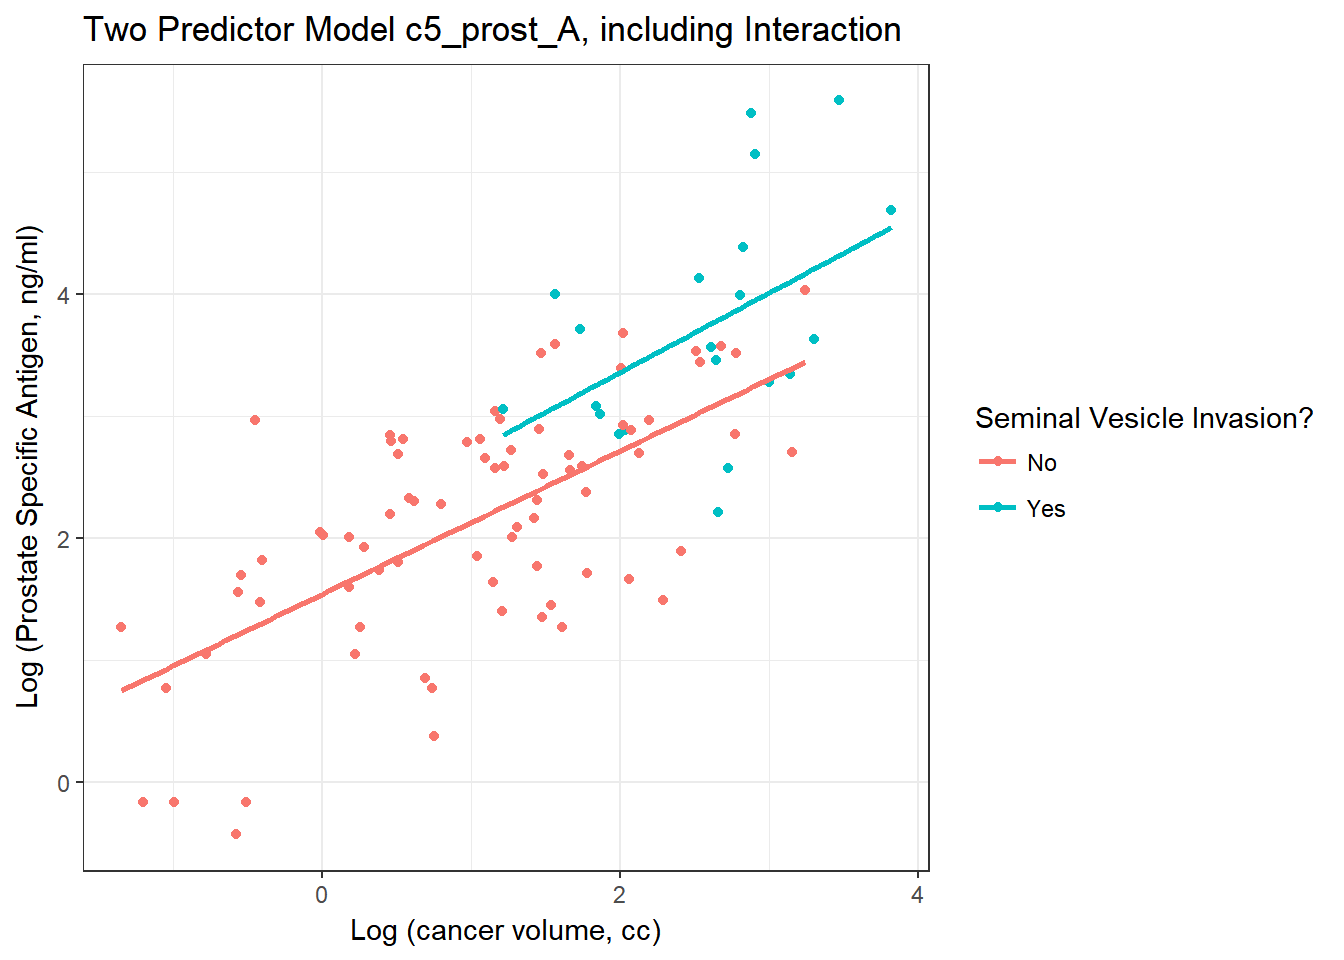
\includegraphics{bookdown-demo_files/figure-latex/unnamed-chunk-53-1.pdf}

\subsubsection{Plot on log-log scale}\label{plot-on-log-log-scale}

Another approach (which might be easier in some settings) would be to
plot the raw values of Cancer Volume and PSA, but use logarithmic axes,
again using the natural (base \emph{e}) logarithm, as follows. If we use
the default choice with `trans = ``log'', we'll find a need to select
some useful break points for the grid, as I've done in what follows.

\begin{Shaded}
\begin{Highlighting}[]
\KeywordTok{ggplot}\NormalTok{(prost, }\KeywordTok{aes}\NormalTok{(}\DataTypeTok{x =}\NormalTok{ cavol, }\DataTypeTok{y =}\NormalTok{ psa, }\DataTypeTok{group =}\NormalTok{ svi_f, }\DataTypeTok{color =}\NormalTok{ svi_f)) }\OperatorTok{+}
\StringTok{    }\KeywordTok{geom_point}\NormalTok{() }\OperatorTok{+}
\StringTok{    }\KeywordTok{geom_smooth}\NormalTok{(}\DataTypeTok{method =} \StringTok{"lm"}\NormalTok{, }\DataTypeTok{se =} \OtherTok{FALSE}\NormalTok{) }\OperatorTok{+}\StringTok{ }
\StringTok{    }\KeywordTok{scale_color_discrete}\NormalTok{(}\DataTypeTok{name =} \StringTok{"Seminal Vesicle Invasion?"}\NormalTok{) }\OperatorTok{+}
\StringTok{    }\KeywordTok{scale_x_continuous}\NormalTok{(}\DataTypeTok{trans =} \StringTok{"log"}\NormalTok{, }
                       \DataTypeTok{breaks =} \KeywordTok{c}\NormalTok{(}\FloatTok{0.5}\NormalTok{, }\DecValTok{1}\NormalTok{, }\DecValTok{2}\NormalTok{, }\DecValTok{5}\NormalTok{, }\DecValTok{10}\NormalTok{, }\DecValTok{25}\NormalTok{, }\DecValTok{50}\NormalTok{)) }\OperatorTok{+}
\StringTok{    }\KeywordTok{scale_y_continuous}\NormalTok{(}\DataTypeTok{trans =} \StringTok{"log"}\NormalTok{, }
                       \DataTypeTok{breaks =} \KeywordTok{c}\NormalTok{(}\DecValTok{1}\NormalTok{, }\DecValTok{2}\NormalTok{, }\DecValTok{4}\NormalTok{, }\DecValTok{10}\NormalTok{, }\DecValTok{25}\NormalTok{, }\DecValTok{50}\NormalTok{, }\DecValTok{100}\NormalTok{, }\DecValTok{200}\NormalTok{)) }\OperatorTok{+}
\StringTok{    }\KeywordTok{theme_bw}\NormalTok{() }\OperatorTok{+}
\StringTok{    }\KeywordTok{labs}\NormalTok{(}\DataTypeTok{x =} \StringTok{"Cancer volume, in cubic centimeters"}\NormalTok{, }
         \DataTypeTok{y =} \StringTok{"Prostate Specific Antigen, in ng/ml"}\NormalTok{, }
         \DataTypeTok{title =} \StringTok{"Two Predictor Model c5_prost_A, including Interaction"}\NormalTok{)}
\end{Highlighting}
\end{Shaded}

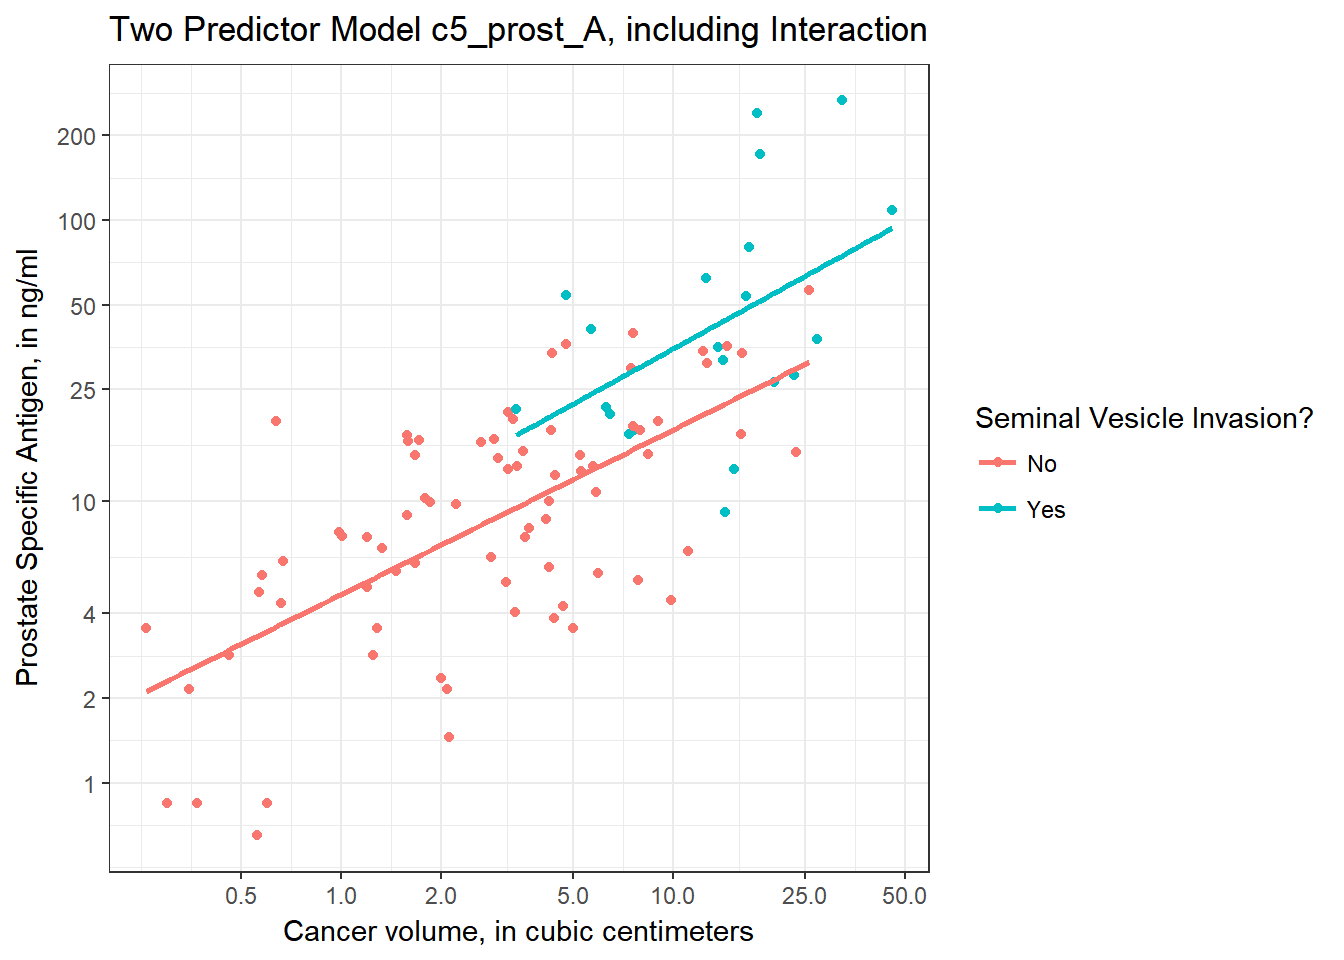
\includegraphics{bookdown-demo_files/figure-latex/unnamed-chunk-54-1.pdf}

I've used the break point of 4 on the Y axis because of the old rule
suggesting further testing for asymptomatic men with PSA of 4 or higher,
but the other break points are arbitrary - they seemed to work for me,
and used round numbers.

\subsection{\texorpdfstring{Residual Plots of
\texttt{c5\_prost\_A}}{Residual Plots of c5\_prost\_A}}\label{residual-plots-of-c5_prost_a}

\begin{Shaded}
\begin{Highlighting}[]
\KeywordTok{plot}\NormalTok{(c5_prost_A, }\DataTypeTok{which =} \DecValTok{1}\NormalTok{)}
\end{Highlighting}
\end{Shaded}

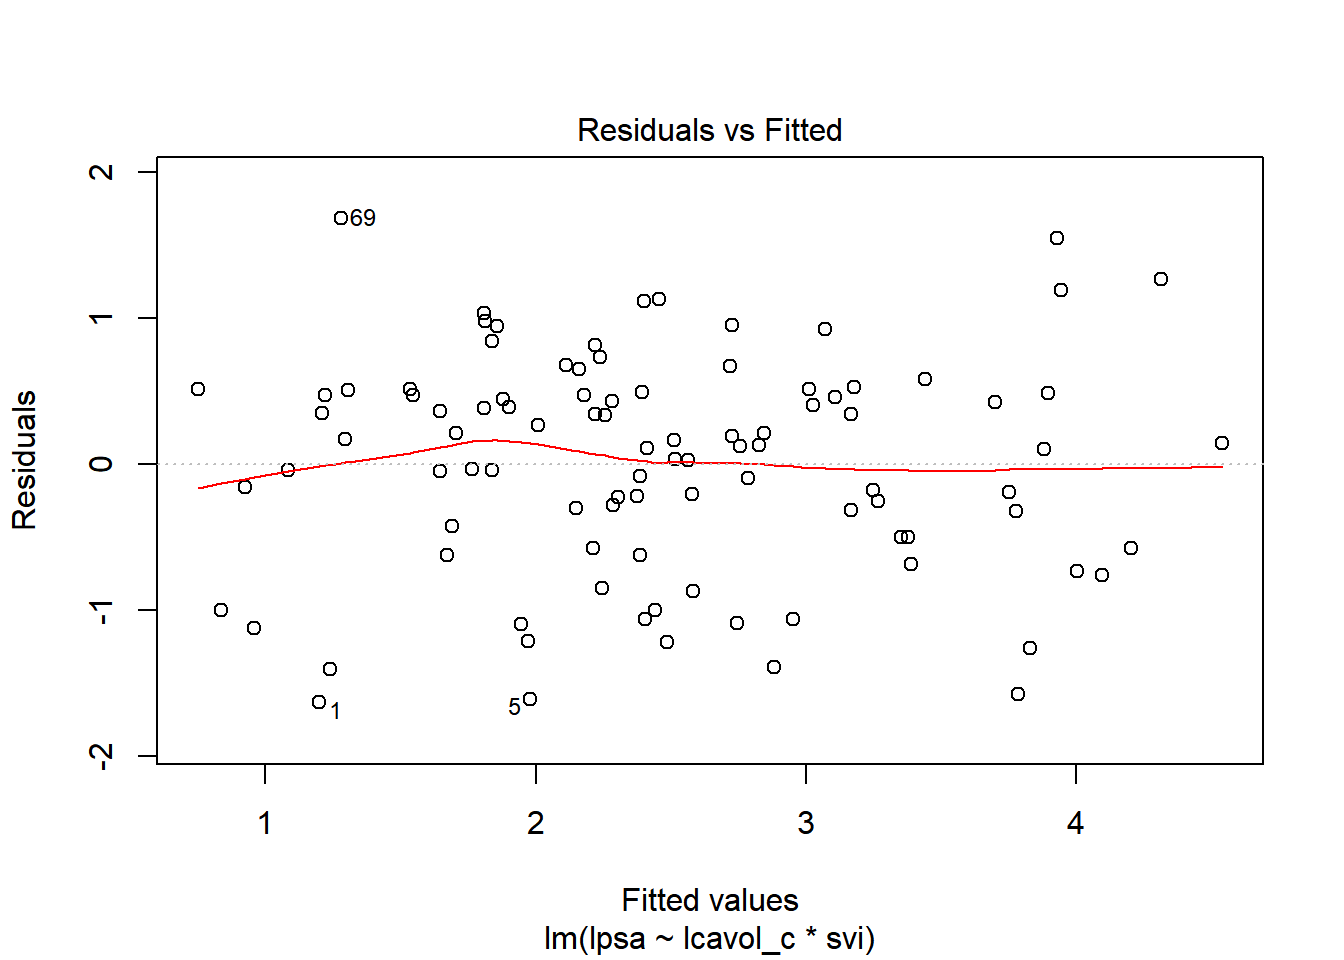
\includegraphics{bookdown-demo_files/figure-latex/unnamed-chunk-55-1.pdf}

\begin{Shaded}
\begin{Highlighting}[]
\KeywordTok{plot}\NormalTok{(c5_prost_A, }\DataTypeTok{which =} \DecValTok{5}\NormalTok{)}
\end{Highlighting}
\end{Shaded}

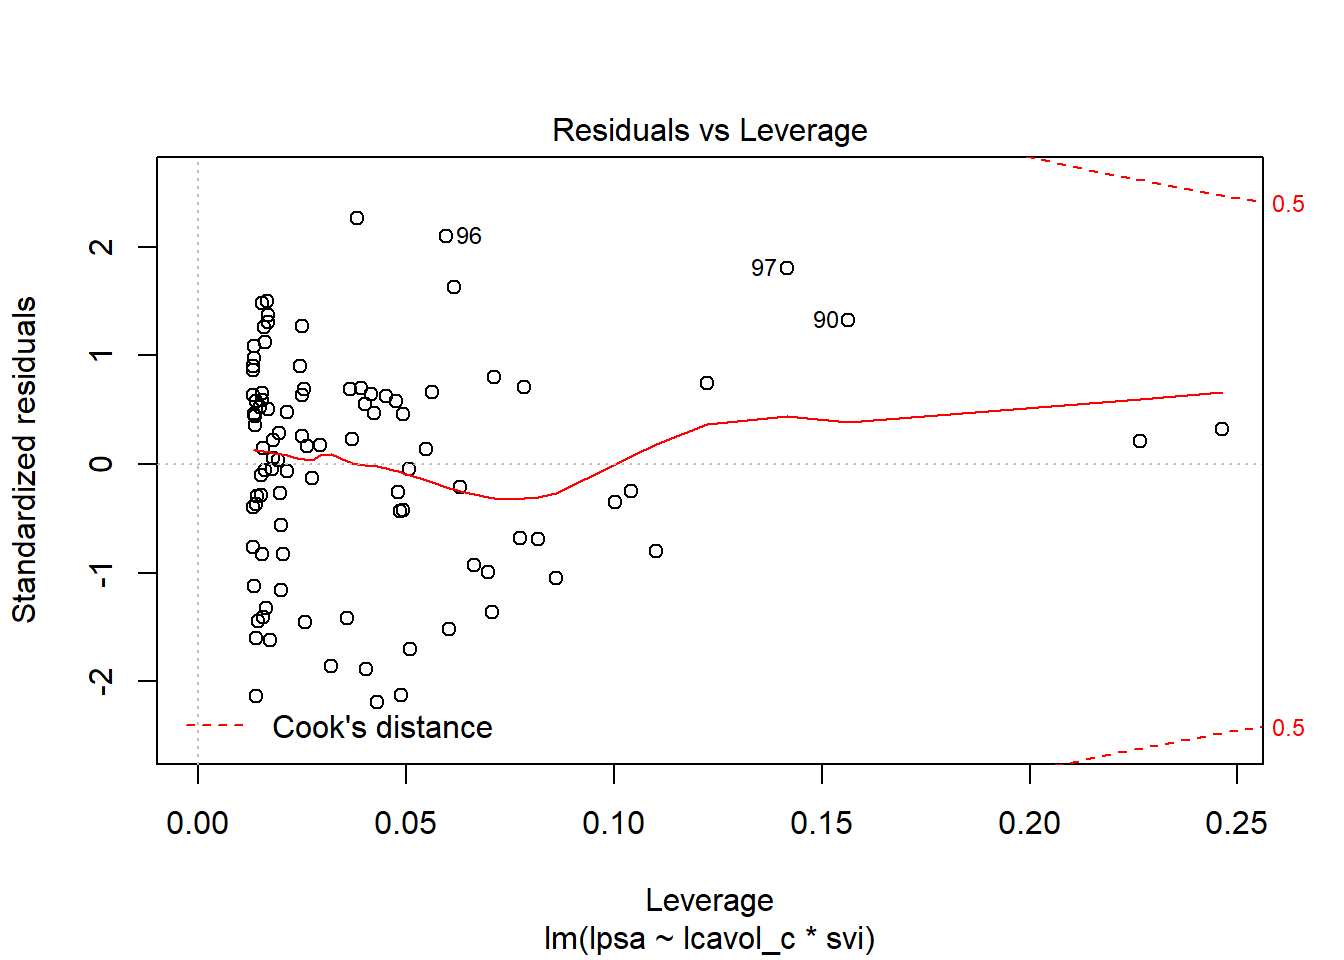
\includegraphics{bookdown-demo_files/figure-latex/unnamed-chunk-56-1.pdf}

\section{\texorpdfstring{Cross-Validation of Model
\texttt{c5\_prost\_A}}{Cross-Validation of Model c5\_prost\_A}}\label{cross-validation-of-model-c5_prost_a}

Suppose we want to evaluate whether our model \texttt{c5\_prost\_A}
predicts effectively in new data.

One approach (used, for instance, in 431) would be to split our sample
into a separate training (perhaps 70\% of the data) and test (perhaps
30\% of the data) samples, and then:

\begin{itemize}
\item
  \begin{enumerate}
  \def\labelenumi{\arabic{enumi}.}
  \tightlist
  \item
    fit the model in the training sample,
  \end{enumerate}
\item
  \begin{enumerate}
  \def\labelenumi{\arabic{enumi}.}
  \setcounter{enumi}{1}
  \tightlist
  \item
    use the resulting model to make predictions for \texttt{lpsa} in the
    test sample, and
  \end{enumerate}
\item
  \begin{enumerate}
  \def\labelenumi{\arabic{enumi}.}
  \setcounter{enumi}{2}
  \tightlist
  \item
    evaluate the quality of those predictions, perhaps by comparing the
    results to what we'd get using a different model.
  \end{enumerate}
\end{itemize}

One problem with this approach is that with a small data set like this,
we may be reluctant to cut our sample size for the training or the
testing down because we're afraid that our model building and testing
will be hampered by a small sample size. A potential solution is the
idea of \textbf{cross-validation}, which involves partitioning our data
into a series of training-test subsets, multiple times, and then
combining the results.

The rest of this section is built on some material by David Robinson at
\url{https://rpubs.com/dgrtwo/cv-modelr}.

Suppose that we want to perform what is called \emph{10-crossfold
separation}. In words, this approach splits the 97 observations in our
\texttt{prost} data frame into 10 exclusive partitions of about 90\% (so
about 87-88 observations) into a training sample, and the remaining 10\%
(9-10 observations) in a test sample\footnote{If we did 5-crossfold
  validation, we'd have 5 partitions into samples of 80\% training and
  20\% test samples.}. We then refit a model of interest using the
training data, and fit the resulting model on the test data using the
\texttt{broom} package's \texttt{augment} function. This process is then
repeated (a total of 10 times) so that each observation is used 9 times
in the training sample, and once in the test sample.

To code this in R, we'll make use of a few new ideas. Our goal will be
to cross-validate model \texttt{c5\_prost\_A}, which, you'll recall,
uses \texttt{lcavol\_c}, \texttt{svi} and their interaction, to predict
\texttt{lpsa} in the \texttt{prost} data.

\begin{enumerate}
\def\labelenumi{\arabic{enumi}.}
\tightlist
\item
  First, we set a seed for the validation algorithm, so we can replicate
  our results down the line.
\item
  Then we use the \texttt{crossv\_kfold} function from the
  \texttt{modelr} package to split the \texttt{prost} data into ten
  different partitions, and then use each partition for a split into
  training and test samples, which the machine indexes with
  \texttt{train} and \texttt{test}.
\item
  Then we use some magic and the \texttt{map} function from the
  \texttt{purrr} package (part of the core \texttt{tidyverse}) to fit a
  new \texttt{lm(lpsa\ \textasciitilde{}\ lcavol\_c\ *\ svi)} model to
  each of the training samples generated by \texttt{crossv\_kfold}.
\item
  Finally, some additional magic with the \texttt{unnest} and
  \texttt{map2} functions applies each of these new models to the
  appropriate test sample, and generate predictions (\texttt{.fitted})
  and standard errors for each prediction (\texttt{.se.fit}).
\end{enumerate}

\begin{Shaded}
\begin{Highlighting}[]
\KeywordTok{set.seed}\NormalTok{(}\DecValTok{4320308}\NormalTok{)}

\NormalTok{prost_models <-}\StringTok{ }\NormalTok{prost }\OperatorTok
\StringTok{    }\KeywordTok{crossv_kfold}\NormalTok{(}\DataTypeTok{k =} \DecValTok{10}\NormalTok{) }\OperatorTok
\StringTok{    }\KeywordTok{mutate}\NormalTok{(}\DataTypeTok{model =} \KeywordTok{map}\NormalTok{(train, }\OperatorTok{~}\StringTok{ }\KeywordTok{lm}\NormalTok{(lpsa }\OperatorTok{~}\StringTok{ }\NormalTok{lcavol_c }\OperatorTok{*}\StringTok{ }\NormalTok{svi, }\DataTypeTok{data =}\NormalTok{ .)))}

\NormalTok{prost_predictions <-}\StringTok{ }\NormalTok{prost_models }\OperatorTok
\StringTok{    }\KeywordTok{unnest}\NormalTok{(}\KeywordTok{map2}\NormalTok{(model, test, }\OperatorTok{~}\StringTok{ }\KeywordTok{augment}\NormalTok{(.x, }\DataTypeTok{newdata =}\NormalTok{ .y)))}

\KeywordTok{head}\NormalTok{(prost_predictions)}
\end{Highlighting}
\end{Shaded}

\begin{verbatim}
# A tibble: 6 x 19
  .id   subject   lpsa   lcavol lweight   age bph      svi    lcp gleason
  <chr>   <int>  <dbl>    <dbl>   <dbl> <int> <fct>  <int>  <dbl> <fct>  
1 01          3 -0.163 -0.511      2.69    74 Low        0 -1.39  7      
2 01         12  1.27  -1.35       3.60    63 Medium     0 -1.39  6      
3 01         16  1.45   1.54       3.06    66 Low        0 -1.39  6      
4 01         18  1.49   2.29       3.65    66 Low        0  0.372 6      
5 01         30  1.89   2.41       3.38    65 Low        0  1.62  6      
6 01         34  2.02   0.00995    3.27    54 Low        0 -1.39  6      
# ... with 9 more variables: pgg45 <int>, svi_f <fct>, gleason_f <fct>,
#   bph_f <fct>, lcavol_c <dbl>, cavol <dbl>, psa <dbl>, .fitted <dbl>,
#   .se.fit <dbl>
\end{verbatim}

The results are a set of predictions based on the splits into training
and test groups (remember there are 10 such splits, indexed by
\texttt{.id}) that describe the complete set of 97 subjects again.

\subsection{Cross-Validated Summaries of Prediction
Quality}\label{cross-validated-summaries-of-prediction-quality}

Now, we can calculate the root Mean Squared Prediction Error (RMSE) and
Mean Absolute Prediction Error (MAE) for this modeling approach (using
\texttt{lcavol\_c} and \texttt{svi} to predict \texttt{lpsa}) across
these observations.

\begin{Shaded}
\begin{Highlighting}[]
\NormalTok{prost_predictions }\OperatorTok
\StringTok{    }\KeywordTok{summarize}\NormalTok{(}\DataTypeTok{RMSE_ourmodel =} \KeywordTok{sqrt}\NormalTok{(}\KeywordTok{mean}\NormalTok{((lpsa }\OperatorTok{-}\StringTok{ }\NormalTok{.fitted) }\OperatorTok{^}\DecValTok{2}\NormalTok{)),}
              \DataTypeTok{MAE_ourmodel =} \KeywordTok{mean}\NormalTok{(}\KeywordTok{abs}\NormalTok{(lpsa }\OperatorTok{-}\StringTok{ }\NormalTok{.fitted)))}
\end{Highlighting}
\end{Shaded}

\begin{verbatim}
# A tibble: 1 x 2
  RMSE_ourmodel MAE_ourmodel
          <dbl>        <dbl>
1         0.783        0.638
\end{verbatim}

For now, we'll compare our model to the ``intercept only'' model that
simply predicts the mean \texttt{lpsa} across all patients.

\begin{Shaded}
\begin{Highlighting}[]
\NormalTok{prost_predictions }\OperatorTok
\StringTok{    }\KeywordTok{summarize}\NormalTok{(}\DataTypeTok{RMSE_intercept =} \KeywordTok{sqrt}\NormalTok{(}\KeywordTok{mean}\NormalTok{((lpsa }\OperatorTok{-}\StringTok{ }\KeywordTok{mean}\NormalTok{(lpsa)) }\OperatorTok{^}\DecValTok{2}\NormalTok{)),}
              \DataTypeTok{MAE_intercept =} \KeywordTok{mean}\NormalTok{(}\KeywordTok{abs}\NormalTok{(lpsa }\OperatorTok{-}\StringTok{ }\KeywordTok{mean}\NormalTok{(lpsa))))}
\end{Highlighting}
\end{Shaded}

\begin{verbatim}
# A tibble: 1 x 2
  RMSE_intercept MAE_intercept
           <dbl>         <dbl>
1           1.15         0.891
\end{verbatim}

So our model looks meaningfully better than the ``intercept only''
model, in that both the RMSE and MAE are much lower (better) with our
model.

Another thing we could do with this tibble of predictions we have
created is to graph the size of the prediction errors (observed
\texttt{lpsa} minus predicted values in \texttt{.fitted}) that our
modeling approach makes.

\begin{Shaded}
\begin{Highlighting}[]
\NormalTok{prost_predictions }\OperatorTok
\StringTok{    }\KeywordTok{mutate}\NormalTok{(}\DataTypeTok{errors =}\NormalTok{ lpsa }\OperatorTok{-}\StringTok{ }\NormalTok{.fitted) }\OperatorTok
\StringTok{    }\KeywordTok{ggplot}\NormalTok{(., }\KeywordTok{aes}\NormalTok{(}\DataTypeTok{x =}\NormalTok{ errors)) }\OperatorTok{+}
\StringTok{    }\KeywordTok{geom_histogram}\NormalTok{(}\DataTypeTok{bins =} \DecValTok{30}\NormalTok{, }\DataTypeTok{fill =} \StringTok{"darkviolet"}\NormalTok{, }\DataTypeTok{col =} \StringTok{"yellow"}\NormalTok{) }\OperatorTok{+}\StringTok{ }
\StringTok{    }\KeywordTok{labs}\NormalTok{(}\DataTypeTok{title =} \StringTok{"Cross-Validated Errors in Prediction of log(PSA)"}\NormalTok{,}
         \DataTypeTok{subtitle =} \StringTok{"Using a model (`c5_prostA`) including lcavol_c and svi and their interaction"}\NormalTok{,}
         \DataTypeTok{x =} \StringTok{"Error in predicting log(PSA)"}\NormalTok{)}
\end{Highlighting}
\end{Shaded}

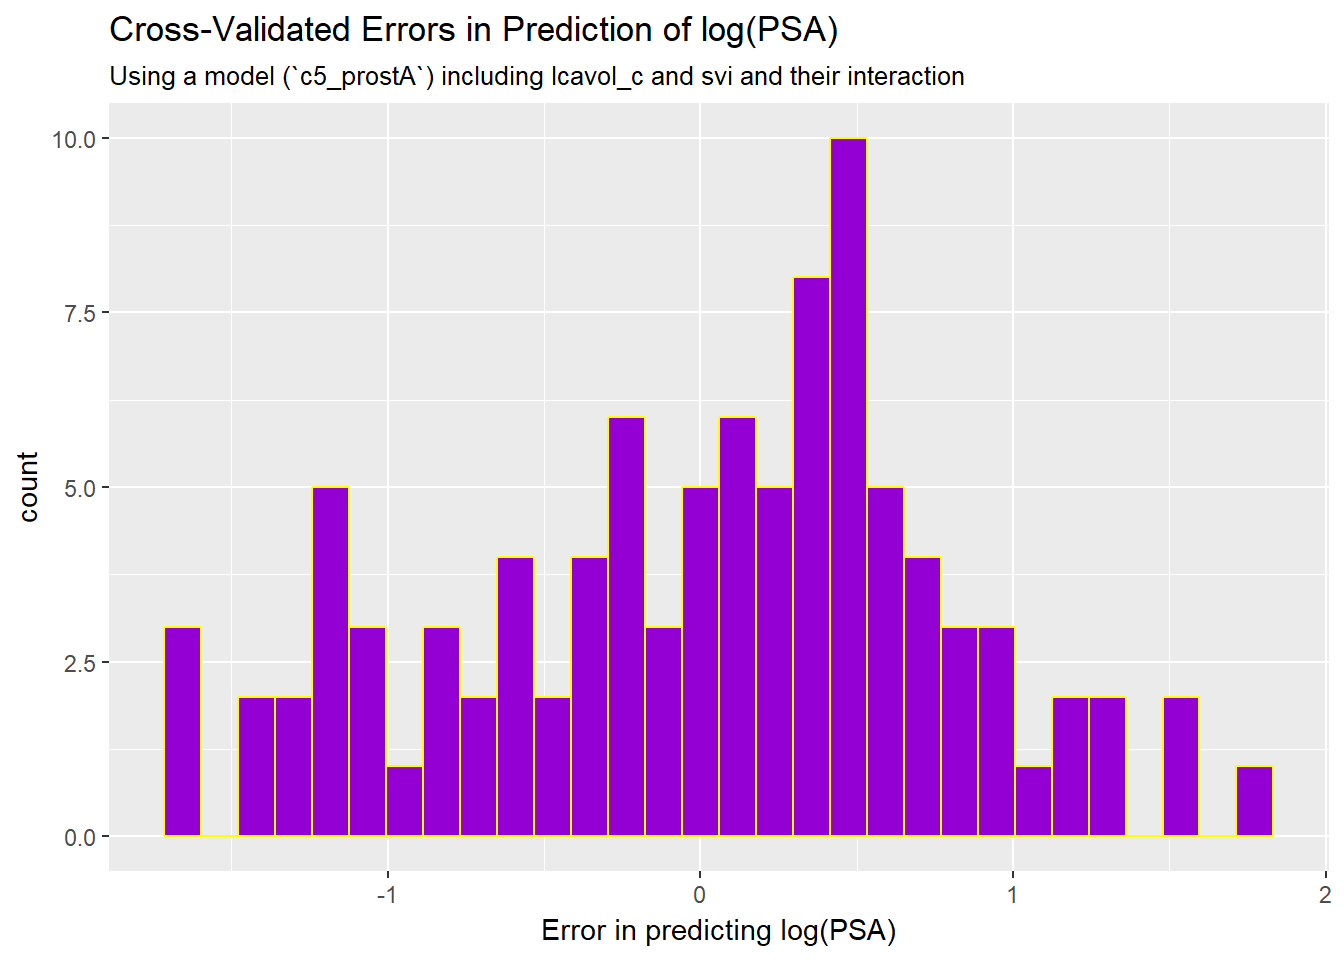
\includegraphics{bookdown-demo_files/figure-latex/validation_c5_prost_A_10fold_errors_histogram-1.pdf}

This suggests that some of our results are off by quite a bit, on the
log(PSA) scale, which is summarized for the original data below.

\begin{Shaded}
\begin{Highlighting}[]
\NormalTok{prost }\OperatorTok\StringTok{ }\KeywordTok{skim}\NormalTok{(lpsa)}
\end{Highlighting}
\end{Shaded}

\begin{verbatim}
Skim summary statistics
 n obs: 97 
 n variables: 16 

Variable type: numeric 
 variable missing complete  n mean   sd    p0  p25 median  p75 p100
     lpsa       0       97 97 2.48 1.15 -0.43 1.73   2.59 3.06 5.58
\end{verbatim}

If we like, we could transform the predictions and observed values back
to the scale of PSA (unlogged) and then calculate and display errors, as
follows:

\begin{Shaded}
\begin{Highlighting}[]
\NormalTok{prost_predictions }\OperatorTok
\StringTok{    }\KeywordTok{mutate}\NormalTok{(}\DataTypeTok{err.psa =} \KeywordTok{exp}\NormalTok{(lpsa) }\OperatorTok{-}\StringTok{ }\KeywordTok{exp}\NormalTok{(.fitted)) }\OperatorTok
\StringTok{    }\KeywordTok{ggplot}\NormalTok{(., }\KeywordTok{aes}\NormalTok{(}\DataTypeTok{x =}\NormalTok{ err.psa)) }\OperatorTok{+}
\StringTok{    }\KeywordTok{geom_histogram}\NormalTok{(}\DataTypeTok{bins =} \DecValTok{30}\NormalTok{, }\DataTypeTok{fill =} \StringTok{"darkorange"}\NormalTok{, }\DataTypeTok{col =} \StringTok{"yellow"}\NormalTok{) }\OperatorTok{+}\StringTok{ }
\StringTok{    }\KeywordTok{labs}\NormalTok{(}\DataTypeTok{title =} \StringTok{"Cross-Validated Errors in Prediction of PSA"}\NormalTok{,}
         \DataTypeTok{subtitle =} \StringTok{"Using a model (`c5_prostA`) including lcavol_c and svi and their interaction"}\NormalTok{,}
         \DataTypeTok{x =} \StringTok{"Error in predicting PSA"}\NormalTok{)}
\end{Highlighting}
\end{Shaded}

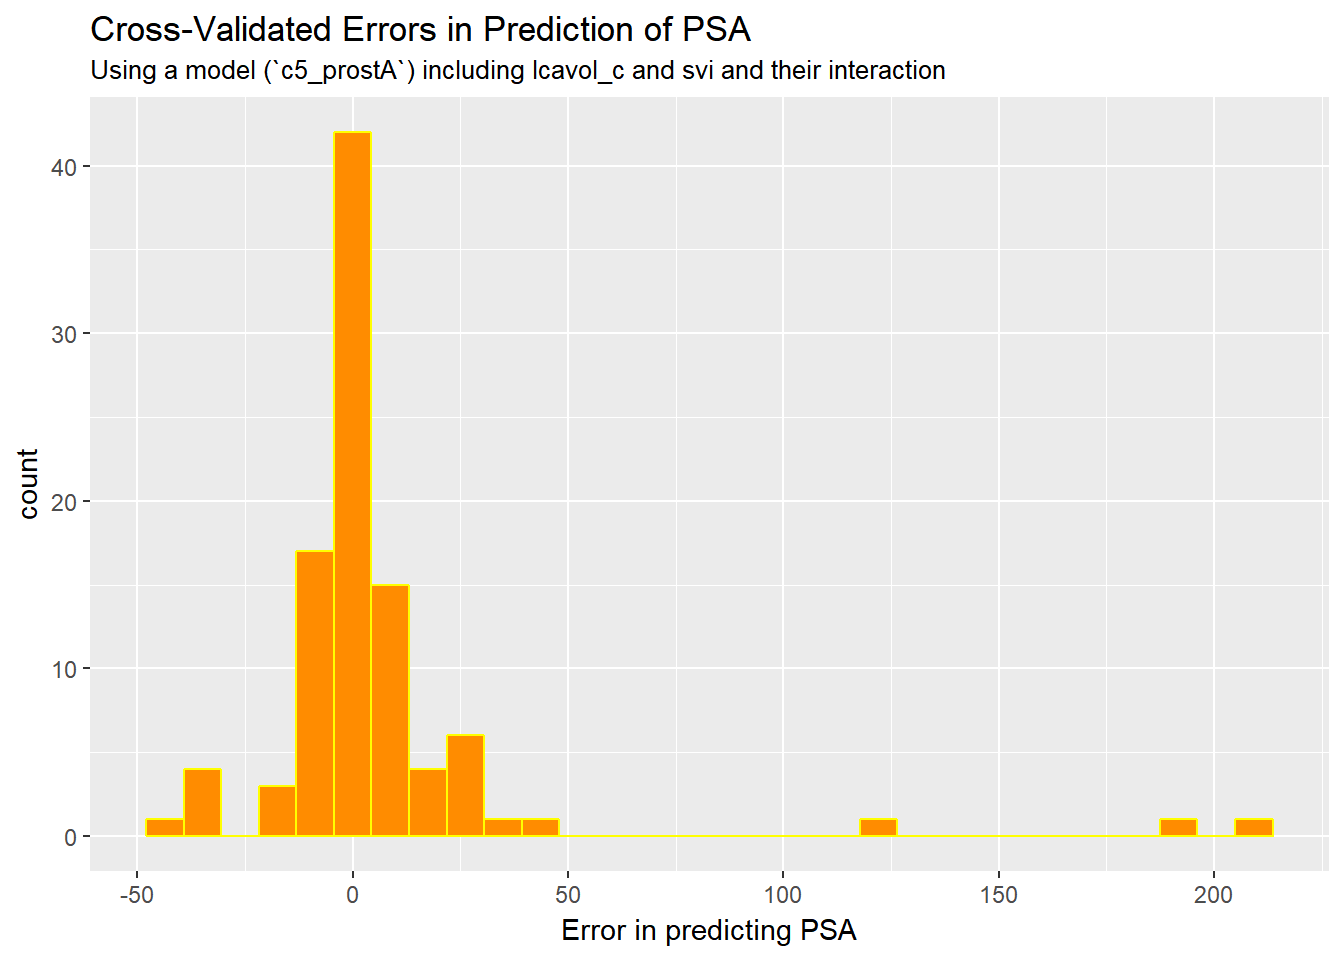
\includegraphics{bookdown-demo_files/figure-latex/validation_c5_prost_A_10fold_errorsonPSA_histogram-1.pdf}

This suggests that some of our results are off by quite a bit, on the
original scale of PSA, which is summarized below.

\begin{Shaded}
\begin{Highlighting}[]
\NormalTok{prost }\OperatorTok\StringTok{ }\KeywordTok{mutate}\NormalTok{(}\DataTypeTok{psa =} \KeywordTok{exp}\NormalTok{(lpsa)) }\OperatorTok\StringTok{ }\KeywordTok{skim}\NormalTok{(psa)}
\end{Highlighting}
\end{Shaded}

\begin{verbatim}
Skim summary statistics
 n obs: 97 
 n variables: 16 

Variable type: numeric 
 variable missing complete  n  mean    sd   p0  p25 median   p75   p100
      psa       0       97 97 23.74 40.83 0.65 5.65  13.35 21.25 265.85
\end{verbatim}

We'll return to the notion of cross-validation again, but for now, let's
consider the problem of considering adding more predictors to our model,
and then making sensible selections as to which predictors actually
should be incorporated.

\chapter{Stepwise Variable Selection}\label{stepwise-variable-selection}

\section{Strategy for Model
Selection}\label{strategy-for-model-selection}

\citet{RamseySchafer2002} suggest a strategy for dealing with many
potential explanatory variables should include the following elements:

\begin{enumerate}
\def\labelenumi{\arabic{enumi}.}
\tightlist
\item
  Identify the key objectives.
\item
  Screen the available variables, deciding on a list that is sensitive
  to the objectives and excludes obvious redundancies.
\item
  Perform exploratory analysis, examining graphical displays and
  correlation coefficients.
\item
  Perform transformations, as necessary.
\item
  Examine a residual plot after fitting a rich model, performing further
  transformations and considering outliers.
\item
  Find a suitable subset of the predictors, exerting enough control over
  any semi-automated selection procedure to be sensitive to the
  questions of interest.
\item
  Proceed with the analysis, using the selected explanatory variables.
\end{enumerate}

The Two Key Aspects of Model Selection are:

\begin{enumerate}
\def\labelenumi{\arabic{enumi}.}
\tightlist
\item
  Evaluating each potential subset of predictor variables
\item
  Deciding on the collection of potential subsets
\end{enumerate}

\subsection{How Do We Choose Potential Subsets of
Predictors?}\label{how-do-we-choose-potential-subsets-of-predictors}

Choosing potential subsets of predictor variables usually involves
either:

\begin{enumerate}
\def\labelenumi{\arabic{enumi}.}
\tightlist
\item
  Stepwise approaches
\item
  All possible subset (or best possible subset) searches
\end{enumerate}

Note that the use of any variable selection procedure changes the
properties of \ldots{}

\begin{itemize}
\tightlist
\item
  the estimated coefficients, which are biased, and
\item
  the associated tests and confidence intervals, which are overly
  optimistic.
\end{itemize}

\citet{Leeb2005} summarize the key issues:

\begin{enumerate}
\def\labelenumi{\arabic{enumi}.}
\tightlist
\item
  Regardless of sample size, the model selection step typically has a
  dramatic effect on the sampling properties of the estimators that
  cannot be ignored. In particular, the sampling properties of
  post-model-selection estimators are typically significantly different
  from the nominal distributions that arise if a fixed model is
  supposed.
\item
  As a consequence, use of inference procedures that do not take into
  account the model selection step (e.g.~using standard t-intervals as
  if the selected model has been given prior to the statistical
  analysis) can be highly misleading.
\end{enumerate}

\section{\texorpdfstring{A ``Kitchen Sink'' Model (Model
\texttt{c5\_prost\_ks})}{A Kitchen Sink Model (Model c5\_prost\_ks)}}\label{a-kitchen-sink-model-model-c5_prost_ks}

Suppose that we now consider a model for the \texttt{prost} data we have
been working with, which includes main effects (and, in this case, only
the main effects) of all eight candidate predictors for \texttt{lpsa},
as follows.

\begin{Shaded}
\begin{Highlighting}[]
\NormalTok{c5_prost_ks <-}\StringTok{ }\KeywordTok{lm}\NormalTok{(lpsa }\OperatorTok{~}\StringTok{ }\NormalTok{lcavol }\OperatorTok{+}\StringTok{ }\NormalTok{lweight }\OperatorTok{+}\StringTok{ }\NormalTok{age }\OperatorTok{+}\StringTok{ }\NormalTok{bph_f }\OperatorTok{+}\StringTok{ }\NormalTok{svi_f }\OperatorTok{+}\StringTok{ }
\StringTok{                }\NormalTok{lcp }\OperatorTok{+}\StringTok{ }\NormalTok{gleason_f }\OperatorTok{+}\StringTok{ }\NormalTok{pgg45, }\DataTypeTok{data =}\NormalTok{ prost)}

\KeywordTok{tidy}\NormalTok{(c5_prost_ks)}
\end{Highlighting}
\end{Shaded}

\begin{verbatim}
          term     estimate   std.error  statistic      p.value
1  (Intercept)  0.169937821 0.931332512  0.1824674 8.556454e-01
2       lcavol  0.544313829 0.087979210  6.1868461 2.010505e-08
3      lweight  0.702237531 0.203013089  3.4590751 8.455164e-04
4          age -0.023857982 0.011081414 -2.1529727 3.412099e-02
5  bph_fMedium  0.364036274 0.182575941  1.9938896 4.933267e-02
6    bph_fHigh  0.248789989 0.195975792  1.2694935 2.076898e-01
7     svi_fYes  0.710949408 0.241990241  2.9379259 4.240326e-03
8          lcp -0.119311781 0.089458946 -1.3337043 1.858223e-01
9   gleason_f7  0.220746268 0.343065609  0.6434520 5.216430e-01
10  gleason_f6 -0.053096704 0.430098039 -0.1234526 9.020368e-01
11       pgg45  0.003984574 0.004146495  0.9609499 3.392714e-01
\end{verbatim}

\begin{Shaded}
\begin{Highlighting}[]
\KeywordTok{glance}\NormalTok{(c5_prost_ks)}
\end{Highlighting}
\end{Shaded}

\begin{verbatim}
  r.squared adj.r.squared     sigma statistic      p.value df    logLik
1 0.6790343     0.6417127 0.6909479  18.19414 2.373796e-17 11 -95.93939
       AIC      BIC deviance df.residual
1 215.8788 246.7753 41.05718          86
\end{verbatim}

We'll often refer to this (all predictors on board) approach as a
``kitchen sink'' model{[}This refers to the English idiom ``\ldots{}
everything but the kitchen sink'' which describes, essentially,
everything imaginable. A ``kitchen sink regression'' is often used as a
pejorative term, since no special skill or insight is required to
identify it, given a list of potential predictors. For more, yes, there
is a
\href{https://en.wikipedia.org/wiki/Kitchen_sink_regression}{Wikipedia
page}.{]}.

\section{Sequential Variable Selection: Stepwise
Approaches}\label{sequential-variable-selection-stepwise-approaches}

\begin{itemize}
\tightlist
\item
  Forward Selection

  \begin{itemize}
  \tightlist
  \item
    We begin with a constant mean and then add potential predictors one
    at a time according to some criterion (R defaults to minimizing the
    Akaike Information Criterion) until no further addition
    significantly improves the fit.
  \item
    Each categorical factor variable is represented in the regression
    model as a set of indicator variables. In the absence of a good
    reason to do something else, the set is added to the model as a
    single unit, and R does this automatically.
  \end{itemize}
\item
  Backwards Elimination

  \begin{itemize}
  \tightlist
  \item
    Start with the ``kitchen sink'' model and then delete potential
    predictors one at a time.
  \item
    Backwards Elimination is less likely than Forward Selection to omit
    negatively confounded sets of variables, though all stepwise
    procedures have problems.
  \end{itemize}
\item
  Stepwise Regression can also be done by combining these methods.
\end{itemize}

\subsection{The Big Problems with Stepwise
Regression}\label{the-big-problems-with-stepwise-regression}

There is no reason to assume that a single best model can be found.

\begin{itemize}
\tightlist
\item
  The use of forward selection, or backwards elimination, or stepwise
  regression including both procedures, will NOT always find the same
  model.
\item
  It also appears to be essentially useless to try different stepwise
  methods to look for agreement.
\end{itemize}

Users of stepwise regression frequently place all of their attention on
the particular explanatory variables included in the resulting model,
when there's \textbf{no reason} (in most cases) to assume that model is
in any way optimal.

Despite all of its problems, let's use stepwise regression to help
predict \texttt{lpsa} given a subset of the eight predictors in
\texttt{c5\_prost\_ks}.

\section{\texorpdfstring{Forward Selection with the \texttt{step}
function}{Forward Selection with the step function}}\label{forward-selection-with-the-step-function}

\begin{enumerate}
\def\labelenumi{\arabic{enumi}.}
\tightlist
\item
  Specify the null model (intercept only)
\item
  Specify the variables R should consider as predictors (in the scope
  element of the step function)
\item
  Specify forward selection only
\item
  R defaults to using AIC as its stepwise criterion
\end{enumerate}

\begin{Shaded}
\begin{Highlighting}[]
\KeywordTok{with}\NormalTok{(prost, }
     \KeywordTok{step}\NormalTok{(}\KeywordTok{lm}\NormalTok{(lpsa }\OperatorTok{~}\StringTok{ }\DecValTok{1}\NormalTok{), }
     \DataTypeTok{scope=}\NormalTok{(}\OperatorTok{~}\StringTok{ }\NormalTok{lcavol }\OperatorTok{+}\StringTok{ }\NormalTok{lweight }\OperatorTok{+}\StringTok{ }\NormalTok{age }\OperatorTok{+}\StringTok{ }\NormalTok{bph_f }\OperatorTok{+}\StringTok{ }\NormalTok{svi_f }\OperatorTok{+}\StringTok{ }
\StringTok{                }\NormalTok{lcp }\OperatorTok{+}\StringTok{ }\NormalTok{gleason_f }\OperatorTok{+}\StringTok{ }\NormalTok{pgg45), }
     \DataTypeTok{direction=}\StringTok{"forward"}\NormalTok{))}
\end{Highlighting}
\end{Shaded}

\begin{verbatim}
Start:  AIC=28.84
lpsa ~ 1

            Df Sum of Sq     RSS     AIC
+ lcavol     1    69.003  58.915 -44.366
+ svi_f      1    41.011  86.907  -6.658
+ lcp        1    38.528  89.389  -3.926
+ gleason_f  2    30.121  97.796   6.793
+ lweight    1    24.019 103.899  10.665
+ pgg45      1    22.814 105.103  11.783
+ age        1     3.679 124.239  28.007
<none>                   127.918  28.838
+ bph_f      2     4.681 123.237  29.221

Step:  AIC=-44.37
lpsa ~ lcavol

            Df Sum of Sq    RSS     AIC
+ lweight    1    7.1726 51.742 -54.958
+ svi_f      1    5.2375 53.677 -51.397
+ bph_f      2    3.2994 55.615 -45.956
+ pgg45      1    1.6980 57.217 -45.203
+ gleason_f  2    2.7834 56.131 -45.061
<none>                   58.915 -44.366
+ lcp        1    0.6562 58.259 -43.452
+ age        1    0.0025 58.912 -42.370

Step:  AIC=-54.96
lpsa ~ lcavol + lweight

            Df Sum of Sq    RSS     AIC
+ svi_f      1    5.1737 46.568 -63.177
+ pgg45      1    1.8158 49.926 -56.424
+ gleason_f  2    2.6770 49.065 -56.111
<none>                   51.742 -54.958
+ lcp        1    0.8187 50.923 -54.506
+ age        1    0.6456 51.097 -54.176
+ bph_f      2    1.4583 50.284 -53.731

Step:  AIC=-63.18
lpsa ~ lcavol + lweight + svi_f

            Df Sum of Sq    RSS     AIC
<none>                   46.568 -63.177
+ gleason_f  2   1.60467 44.964 -62.579
+ age        1   0.62301 45.945 -62.484
+ bph_f      2   1.50046 45.068 -62.354
+ pgg45      1   0.50069 46.068 -62.226
+ lcp        1   0.06937 46.499 -61.322
\end{verbatim}

\begin{verbatim}

Call:
lm(formula = lpsa ~ lcavol + lweight + svi_f)

Coefficients:
(Intercept)       lcavol      lweight     svi_fYes  
    -0.7772       0.5259       0.6618       0.6657  
\end{verbatim}

The resulting model, arrived at after three forward selection steps,
includes \texttt{lcavol}, \texttt{lweight} and \texttt{svi\_f}.

\begin{Shaded}
\begin{Highlighting}[]
\NormalTok{model.fs <-}\StringTok{ }\KeywordTok{lm}\NormalTok{(lpsa }\OperatorTok{~}\StringTok{ }\NormalTok{lcavol }\OperatorTok{+}\StringTok{ }\NormalTok{lweight }\OperatorTok{+}\StringTok{ }\NormalTok{svi_f, }
               \DataTypeTok{data=}\NormalTok{prost)}
\KeywordTok{summary}\NormalTok{(model.fs)}\OperatorTok{$}\NormalTok{adj.r.squared}
\end{Highlighting}
\end{Shaded}

\begin{verbatim}
[1] 0.6242063
\end{verbatim}

\begin{Shaded}
\begin{Highlighting}[]
\KeywordTok{extractAIC}\NormalTok{(model.fs)}
\end{Highlighting}
\end{Shaded}

\begin{verbatim}
[1]   4.00000 -63.17744
\end{verbatim}

The adjusted R\textsuperscript{2} value for this model is 0.624, and the
AIC value used by the stepwise procedure is -63.18, on 4 effective
degrees of freedom.

\section{\texorpdfstring{Backward Elimination using the \texttt{step}
function}{Backward Elimination using the step function}}\label{backward-elimination-using-the-step-function}

In this case, the backward elimination approach, using reduction in AIC
for a criterion, comes to the same conclusion about the ``best'' model.

\begin{Shaded}
\begin{Highlighting}[]
\KeywordTok{with}\NormalTok{(prost, }
     \KeywordTok{step}\NormalTok{(}\KeywordTok{lm}\NormalTok{(lpsa }\OperatorTok{~}\StringTok{ }\NormalTok{lcavol }\OperatorTok{+}\StringTok{ }\NormalTok{lweight }\OperatorTok{+}\StringTok{ }\NormalTok{age }\OperatorTok{+}\StringTok{ }\NormalTok{bph_f }\OperatorTok{+}\StringTok{ }
\StringTok{                 }\NormalTok{svi_f }\OperatorTok{+}\StringTok{ }\NormalTok{lcp }\OperatorTok{+}\StringTok{ }\NormalTok{gleason_f }\OperatorTok{+}\StringTok{ }\NormalTok{pgg45), }
          \DataTypeTok{direction=}\StringTok{"backward"}\NormalTok{))}
\end{Highlighting}
\end{Shaded}

\begin{verbatim}
Start:  AIC=-61.4
lpsa ~ lcavol + lweight + age + bph_f + svi_f + lcp + gleason_f + 
    pgg45

            Df Sum of Sq    RSS     AIC
- gleason_f  2    1.1832 42.240 -62.639
- pgg45      1    0.4409 41.498 -62.359
- lcp        1    0.8492 41.906 -61.409
<none>                   41.057 -61.395
- bph_f      2    2.0299 43.087 -60.714
- age        1    2.2129 43.270 -58.303
- svi_f      1    4.1207 45.178 -54.118
- lweight    1    5.7123 46.769 -50.760
- lcavol     1   18.2738 59.331 -27.683

Step:  AIC=-62.64
lpsa ~ lcavol + lweight + age + bph_f + svi_f + lcp + pgg45

          Df Sum of Sq    RSS     AIC
- lcp      1    0.8470 43.087 -62.713
<none>                 42.240 -62.639
- pgg45    1    1.2029 43.443 -61.916
- bph_f    2    2.2515 44.492 -61.602
- age      1    2.0730 44.313 -59.992
- svi_f    1    4.6431 46.884 -54.523
- lweight  1    5.5988 47.839 -52.566
- lcavol   1   21.4956 63.736 -24.736

Step:  AIC=-62.71
lpsa ~ lcavol + lweight + age + bph_f + svi_f + pgg45

          Df Sum of Sq    RSS     AIC
- pgg45    1    0.5860 43.673 -63.403
<none>                 43.087 -62.713
- bph_f    2    2.0214 45.109 -62.266
- age      1    1.7101 44.798 -60.938
- svi_f    1    3.7964 46.884 -56.523
- lweight  1    5.6462 48.734 -52.769
- lcavol   1   22.5152 65.603 -23.936

Step:  AIC=-63.4
lpsa ~ lcavol + lweight + age + bph_f + svi_f

          Df Sum of Sq    RSS     AIC
<none>                 43.673 -63.403
- bph_f    2    2.2720 45.945 -62.484
- age      1    1.3945 45.068 -62.354
- svi_f    1    5.2747 48.948 -54.343
- lweight  1    5.3319 49.005 -54.230
- lcavol   1   25.5538 69.227 -20.720
\end{verbatim}

\begin{verbatim}

Call:
lm(formula = lpsa ~ lcavol + lweight + age + bph_f + svi_f)

Coefficients:
(Intercept)       lcavol      lweight          age  bph_fMedium  
    0.14329      0.54022      0.67283     -0.01819      0.37607  
  bph_fHigh     svi_fYes  
    0.27216      0.68174  
\end{verbatim}

The backwards elimination approach in this case lands on a model with
five inputs (one of which includes two \texttt{bph} indicators,)
eliminating only \texttt{gleason\_f}, \texttt{pgg45} and \texttt{lcp}.

\section{Allen-Cady Modified Backward
Elimination}\label{allen-cady-modified-backward-elimination}

Ranking candidate predictors by importance in advance of backwards
elimination can help avoid false-positives, while reducing model size.
See \citet{Vittinghoff2012}, Section 10.3 for more details.

\begin{enumerate}
\def\labelenumi{\arabic{enumi}.}
\tightlist
\item
  First, force into the model any predictors of primary interest, and
  any confounders necessary for face validity of the final model.

  \begin{itemize}
  \tightlist
  \item
    ``Some variables in the hypothesized causal model may be such
    well-established causal antecedents of the outcome that it makes
    sense to include them, essentially to establish the face validity of
    the model and without regard to the strength or statistical
    significance of their associations with the primary predictor and
    outcome \ldots{}''
  \end{itemize}
\item
  Rank the remaining candidate predictors in order of importance.
\item
  Starting from an initial model with all candidate predictors included,
  delete predictors in order of ascending importance until the first
  variable meeting a criterion to stay in the model hits. Then stop.
\end{enumerate}

Only the remaining variable hypothesized to be least important is
eligible for removal at each step. When we are willing to do this
sorting before collecting (or analyzing) the data, then we can do
Allen-Cady backwards elimination using the \texttt{drop1} command in R.

\subsection{Demonstration of the Allen-Cady
approach}\label{demonstration-of-the-allen-cady-approach}

Suppose, for the moment that we decided to fit a model for the log of
\texttt{psa} and we decided (before we saw the data) that we would:

lcavol + lweight + svi\_f + age + bph\_f + gleason\_f + lcp + pgg45

\begin{itemize}
\tightlist
\item
  force the \texttt{gleason\_f} variable to be in the model, due to
  prior information about its importance,
\item
  and then rated the importance of the other variables as
  \texttt{lcavol} (most important), then \texttt{svi\_f} then
  \texttt{age}, and then \texttt{bph\_f}, then \texttt{lweight} and
  \texttt{lcp} followed by \texttt{pgg45} (least important)
\end{itemize}

When we are willing to do this sorting before collecting (or analyzing)
the data, then we can do Allen-Cady backwards elimination using the
\texttt{drop1} command in R.

\textbf{Step 1.} Fit the full model, then see if removing \texttt{pgg45}
improves AIC\ldots{}

\begin{Shaded}
\begin{Highlighting}[]
\KeywordTok{with}\NormalTok{(prost, }\KeywordTok{drop1}\NormalTok{(}\KeywordTok{lm}\NormalTok{(lpsa }\OperatorTok{~}\StringTok{ }\NormalTok{gleason_f }\OperatorTok{+}\StringTok{ }\NormalTok{lcavol }\OperatorTok{+}\StringTok{ }\NormalTok{svi_f }\OperatorTok{+}\StringTok{ }
\StringTok{              }\NormalTok{age }\OperatorTok{+}\StringTok{ }\NormalTok{bph_f }\OperatorTok{+}\StringTok{ }\NormalTok{lweight }\OperatorTok{+}\StringTok{ }\NormalTok{lcp }\OperatorTok{+}\StringTok{ }\NormalTok{pgg45),}
              \DataTypeTok{scope =}\NormalTok{ (}\OperatorTok{~}\StringTok{ }\NormalTok{pgg45)))}
\end{Highlighting}
\end{Shaded}

\begin{verbatim}
Single term deletions

Model:
lpsa ~ gleason_f + lcavol + svi_f + age + bph_f + lweight + lcp + 
    pgg45
       Df Sum of Sq    RSS     AIC
<none>              41.057 -61.395
pgg45   1   0.44085 41.498 -62.359
\end{verbatim}

Since -62.3 is smaller (i.e.~more negative) than -61.4, we delete
\texttt{pgg45} and move on to assess whether we can remove the variable
we deemed next least important (\texttt{lcp})

\textbf{Step 2.} Let's see if removing \texttt{lcp} from this model
improves AIC\ldots{}

\begin{Shaded}
\begin{Highlighting}[]
\KeywordTok{with}\NormalTok{(prost, }\KeywordTok{drop1}\NormalTok{(}\KeywordTok{lm}\NormalTok{(lpsa }\OperatorTok{~}\StringTok{ }\NormalTok{gleason_f }\OperatorTok{+}\StringTok{ }\NormalTok{lcavol }\OperatorTok{+}\StringTok{ }\NormalTok{svi_f }\OperatorTok{+}\StringTok{ }
\StringTok{              }\NormalTok{age }\OperatorTok{+}\StringTok{ }\NormalTok{bph_f }\OperatorTok{+}\StringTok{ }\NormalTok{lweight  }\OperatorTok{+}\StringTok{ }\NormalTok{lcp),}
              \DataTypeTok{scope =}\NormalTok{ (}\OperatorTok{~}\StringTok{ }\NormalTok{lcp)))}
\end{Highlighting}
\end{Shaded}

\begin{verbatim}
Single term deletions

Model:
lpsa ~ gleason_f + lcavol + svi_f + age + bph_f + lweight + lcp
       Df Sum of Sq    RSS     AIC
<none>              41.498 -62.359
lcp     1   0.56767 42.066 -63.041
\end{verbatim}

Again, since -63.0 is smaller than -62.4, we delete \texttt{lcp} and
next assess whether we should delete \texttt{lweight}.

\textbf{Step 3.} Does removing \texttt{lweight} from this model improves
AIC\ldots{}

\begin{Shaded}
\begin{Highlighting}[]
\KeywordTok{with}\NormalTok{(prost, }\KeywordTok{drop1}\NormalTok{(}\KeywordTok{lm}\NormalTok{(lpsa }\OperatorTok{~}\StringTok{ }\NormalTok{gleason_f }\OperatorTok{+}\StringTok{ }\NormalTok{lcavol }\OperatorTok{+}\StringTok{ }\NormalTok{svi_f }\OperatorTok{+}\StringTok{ }
\StringTok{              }\NormalTok{age }\OperatorTok{+}\StringTok{ }\NormalTok{bph_f }\OperatorTok{+}\StringTok{ }\NormalTok{lweight),}
              \DataTypeTok{scope =}\NormalTok{ (}\OperatorTok{~}\StringTok{ }\NormalTok{lweight)))}
\end{Highlighting}
\end{Shaded}

\begin{verbatim}
Single term deletions

Model:
lpsa ~ gleason_f + lcavol + svi_f + age + bph_f + lweight
        Df Sum of Sq    RSS     AIC
<none>               42.066 -63.041
lweight  1     5.678 47.744 -52.760
\end{verbatim}

Since the AIC for the model after the removal of \texttt{lweight} is
larger (i.e.~less negative), we stop, and declare our final model by the
Allen-Cady approach to include \texttt{gleason\_f}, \texttt{lcavol},
\texttt{svi\_f}, \texttt{age}, \texttt{bph\_f} and \texttt{lweight}.

\section{Summarizing the Results}\label{summarizing-the-results}

\begin{longtable}[]{@{}rl@{}}
\toprule
Method & Suggested Predictors\tabularnewline
\midrule
\endhead
Forward selection & \texttt{lcavol}, \texttt{lweight},
\texttt{svi\_f}\tabularnewline
Backwards elimination & \texttt{lcavol}, \texttt{lweight},
\texttt{svi\_f}, \texttt{age}, \texttt{bph\_f}\tabularnewline
Allen-Cady approach & \texttt{lcavol}, \texttt{lweight},
\texttt{svi\_f}, \texttt{age}, \texttt{bph\_f},
\texttt{gleason\_f}\tabularnewline
\bottomrule
\end{longtable}

\subsection{In-Sample Testing and
Summaries}\label{in-sample-testing-and-summaries}

Since these models are nested in each other, let's look at the summary
statistics (like R\textsuperscript{2}, and AIC) and also run an
ANOVA-based comparison of these nested models to each other and to the
model with the intercept alone, and the kitchen sink model with all
available predictors.

\begin{Shaded}
\begin{Highlighting}[]
\NormalTok{prost_m_int <-}\StringTok{ }\KeywordTok{lm}\NormalTok{(lpsa }\OperatorTok{~}\StringTok{ }\DecValTok{1}\NormalTok{, }\DataTypeTok{data =}\NormalTok{ prost)}
\NormalTok{prost_m_fw <-}\StringTok{ }\KeywordTok{lm}\NormalTok{(lpsa }\OperatorTok{~}\StringTok{ }\NormalTok{lcavol }\OperatorTok{+}\StringTok{ }\NormalTok{lweight }\OperatorTok{+}\StringTok{ }\NormalTok{svi_f, }\DataTypeTok{data =}\NormalTok{ prost)}
\NormalTok{prost_m_bw <-}\StringTok{ }\KeywordTok{lm}\NormalTok{(lpsa }\OperatorTok{~}\StringTok{ }\NormalTok{lcavol }\OperatorTok{+}\StringTok{ }\NormalTok{lweight }\OperatorTok{+}\StringTok{ }\NormalTok{svi_f }\OperatorTok{+}\StringTok{ }
\StringTok{              }\NormalTok{age }\OperatorTok{+}\StringTok{ }\NormalTok{bph_f }\OperatorTok{+}\StringTok{ }\NormalTok{gleason_f, }\DataTypeTok{data =}\NormalTok{ prost)}
\NormalTok{prost_m_ac <-}\StringTok{ }\KeywordTok{lm}\NormalTok{(lpsa }\OperatorTok{~}\StringTok{ }\NormalTok{lcavol }\OperatorTok{+}\StringTok{ }\NormalTok{lweight }\OperatorTok{+}\StringTok{ }\NormalTok{svi_f }\OperatorTok{+}\StringTok{ }
\StringTok{              }\NormalTok{age }\OperatorTok{+}\StringTok{ }\NormalTok{bph_f }\OperatorTok{+}\StringTok{ }\NormalTok{gleason_f }\OperatorTok{+}\StringTok{ }\NormalTok{lcp, }\DataTypeTok{data =}\NormalTok{ prost)}
\NormalTok{prost_m_ks <-}\StringTok{ }\KeywordTok{lm}\NormalTok{(lpsa }\OperatorTok{~}\StringTok{ }\NormalTok{lcavol }\OperatorTok{+}\StringTok{ }\NormalTok{lweight }\OperatorTok{+}\StringTok{ }\NormalTok{svi_f }\OperatorTok{+}\StringTok{ }
\StringTok{              }\NormalTok{age }\OperatorTok{+}\StringTok{ }\NormalTok{bph_f }\OperatorTok{+}\StringTok{ }\NormalTok{gleason_f }\OperatorTok{+}\StringTok{ }\NormalTok{lcp }\OperatorTok{+}\StringTok{ }\NormalTok{pgg45, }\DataTypeTok{data =}\NormalTok{ prost)}
\end{Highlighting}
\end{Shaded}

\subsubsection{\texorpdfstring{Model Fit Summaries (in-sample) from
\texttt{glance}}{Model Fit Summaries (in-sample) from glance}}\label{model-fit-summaries-in-sample-from-glance}

Here are the models, at a \texttt{glance} from the \texttt{broom}
package.

\begin{Shaded}
\begin{Highlighting}[]
\NormalTok{prost_sum <-}\StringTok{ }\KeywordTok{bind_rows}\NormalTok{(}\KeywordTok{glance}\NormalTok{(prost_m_int), }\KeywordTok{glance}\NormalTok{(prost_m_fw),}
                       \KeywordTok{glance}\NormalTok{(prost_m_bw), }\KeywordTok{glance}\NormalTok{(prost_m_ac), }
                       \KeywordTok{glance}\NormalTok{(prost_m_ks)) }\OperatorTok\StringTok{ }\KeywordTok{round}\NormalTok{(., }\DecValTok{3}\NormalTok{)}
\NormalTok{prost_sum}\OperatorTok{$}\NormalTok{names <-}\StringTok{ }\KeywordTok{c}\NormalTok{(}\StringTok{"intercept"}\NormalTok{, }\StringTok{"lcavol + lweight + svi"}\NormalTok{, }
                      \StringTok{"... + age + bhp + gleason"}\NormalTok{, }\StringTok{"... + lcp"}\NormalTok{, }\StringTok{"... + pgg45"}\NormalTok{)}
\NormalTok{prost_sum <-}\StringTok{ }\NormalTok{prost_sum }\OperatorTok
\StringTok{    }\KeywordTok{select}\NormalTok{(names, r.squared, adj.r.squared, AIC, BIC, sigma, df, df.residual)}

\NormalTok{prost_sum}
\end{Highlighting}
\end{Shaded}

\begin{verbatim}
                      names r.squared adj.r.squared     AIC     BIC sigma
1                 intercept     0.000         0.000 306.112 311.261 1.154
2    lcavol + lweight + svi     0.636         0.624 214.097 226.970 0.708
3 ... + age + bhp + gleason     0.671         0.641 214.233 239.980 0.691
4                 ... + lcp     0.676         0.642 214.915 243.237 0.691
5               ... + pgg45     0.679         0.642 215.879 246.775 0.691
  df df.residual
1  1          96
2  4          93
3  9          88
4 10          87
5 11          86
\end{verbatim}

From these summaries, it looks like:

\begin{itemize}
\tightlist
\item
  the adjusted R\textsuperscript{2} is essentially indistinguishable
  between the three largest models, but a bit less strong with the
  three-predictor (4 df) model, and
\item
  the AIC and BIC are (slightly) better (lower) with the three-predictor
  model (4 df) than any other.
\end{itemize}

So we might be motivated by these summaries to select any of the three
models we're studying closely here.

\subsubsection{Model Testing via ANOVA
(in-sample)}\label{model-testing-via-anova-in-sample}

To obtain ANOVA-based test results, we'll run\ldots{}

\begin{Shaded}
\begin{Highlighting}[]
\KeywordTok{anova}\NormalTok{(prost_m_int, prost_m_fw, prost_m_bw, prost_m_ac, prost_m_ks)}
\end{Highlighting}
\end{Shaded}

\begin{verbatim}
Analysis of Variance Table

Model 1: lpsa ~ 1
Model 2: lpsa ~ lcavol + lweight + svi_f
Model 3: lpsa ~ lcavol + lweight + svi_f + age + bph_f + gleason_f
Model 4: lpsa ~ lcavol + lweight + svi_f + age + bph_f + gleason_f + lcp
Model 5: lpsa ~ lcavol + lweight + svi_f + age + bph_f + gleason_f + lcp + 
    pgg45
  Res.Df     RSS Df Sum of Sq       F Pr(>F)    
1     96 127.918                                
2     93  46.568  3    81.349 56.7991 <2e-16 ***
3     88  42.066  5     4.503  1.8863 0.1050    
4     87  41.498  1     0.568  1.1891 0.2786    
5     86  41.057  1     0.441  0.9234 0.3393    
---
Signif. codes:  0 '***' 0.001 '**' 0.01 '*' 0.05 '.' 0.1 ' ' 1
\end{verbatim}

What conclusions can we draw on the basis of these ANOVA tests?

\begin{itemize}
\tightlist
\item
  There is a statistically significant improvement in predictive value
  for Model 2 (the forward selection approach) as compared to Model 1
  (the intercept only.)
\item
  The ANOVA test comparing Model 5 (kitchen sink) to Model 4 (Allen-Cady
  result) shows no statistically significant improvement in predictive
  value.
\item
  Neither does the ANOVA test comparing Model 3 to Model 2 or Model 4 to
  Model 3.
\end{itemize}

This suggests that, \textbf{if we are willing to let the ANOVA test
decide our best model} than that would be the model produced by forward
selection, with predictors \texttt{lcavol}, \texttt{lweight} and
\texttt{svi\_f}. But we haven't validated the models.

\begin{enumerate}
\def\labelenumi{\arabic{enumi}.}
\tightlist
\item
  If the purpose of the model is to predict new data, some sort of
  out-of-sample or cross-validation approach will be necessary, and
\item
  Even if our goal isn't prediction but merely description of the
  current data, we would still want to build diagnostic plots to
  regression assumptions in each model, and
\item
  There is no reason to assume in advance that any of these models is in
  fact correct, or that any one of these stepwise approaches is
  necessarily better than any other, and
\item
  The mere act of running a stepwise regression model, as we'll see, can
  increase the bias in our findings if we accept the results at face
  value.
\end{enumerate}

So we'll need some ways to validate the results once we complete the
selection process.

\subsection{Validating the Results of the Various
Models}\label{validating-the-results-of-the-various-models}

We can use a 5-fold cross-validation approach to assess the predictions
made by our potential models and then compare them. Let's compare our
three models:

\begin{itemize}
\tightlist
\item
  the three predictor model obtained by forward selection, including
  \texttt{lcavol}, \texttt{lweight}, and \texttt{svi\_f}
\item
  the five predictor model obtained by backwards elimination, including
  \texttt{lcavol}, \texttt{lweight}, \texttt{svi\_f}, and also
  \texttt{age}, and \texttt{bph\_f}
\item
  the six predictor model obtained by the Allen-Cady approach, adding
  \texttt{gleason\_f} to the previous model.
\end{itemize}

Here's the 5-fold validation work (and resulting RMSE and MAE estimates)
for the three-predictor model.

\begin{Shaded}
\begin{Highlighting}[]
\KeywordTok{set.seed}\NormalTok{(}\DecValTok{43201012}\NormalTok{)}

\NormalTok{prost3_models <-}\StringTok{ }\NormalTok{prost }\OperatorTok
\StringTok{    }\KeywordTok{crossv_kfold}\NormalTok{(}\DataTypeTok{k =} \DecValTok{5}\NormalTok{) }\OperatorTok
\StringTok{    }\KeywordTok{mutate}\NormalTok{(}\DataTypeTok{model =} \KeywordTok{map}\NormalTok{(train, }\OperatorTok{~}\StringTok{ }\KeywordTok{lm}\NormalTok{(lpsa }\OperatorTok{~}\StringTok{ }\NormalTok{lcavol }\OperatorTok{+}\StringTok{ }\NormalTok{lweight }\OperatorTok{+}\StringTok{ }
\StringTok{                                       }\NormalTok{svi_f, }\DataTypeTok{data =}\NormalTok{ .)))}

\NormalTok{prost3_preds <-}\StringTok{ }\NormalTok{prost3_models }\OperatorTok
\StringTok{    }\KeywordTok{unnest}\NormalTok{(}\KeywordTok{map2}\NormalTok{(model, test, }\OperatorTok{~}\StringTok{ }\KeywordTok{augment}\NormalTok{(.x, }\DataTypeTok{newdata =}\NormalTok{ .y)))}

\NormalTok{prost3_preds }\OperatorTok
\StringTok{    }\KeywordTok{summarize}\NormalTok{(}\DataTypeTok{RMSE_prost3 =} \KeywordTok{sqrt}\NormalTok{(}\KeywordTok{mean}\NormalTok{((lpsa }\OperatorTok{-}\StringTok{ }\NormalTok{.fitted) }\OperatorTok{^}\DecValTok{2}\NormalTok{)),}
              \DataTypeTok{MAE_prost3 =} \KeywordTok{mean}\NormalTok{(}\KeywordTok{abs}\NormalTok{(lpsa }\OperatorTok{-}\StringTok{ }\NormalTok{.fitted)))}
\end{Highlighting}
\end{Shaded}

\begin{verbatim}
# A tibble: 1 x 2
  RMSE_prost3 MAE_prost3
        <dbl>      <dbl>
1       0.745      0.587
\end{verbatim}

Now, we'll generate the RMSE and MAE estimates for the five-predictor
model.

\begin{Shaded}
\begin{Highlighting}[]
\KeywordTok{set.seed}\NormalTok{(}\DecValTok{43206879}\NormalTok{)}

\NormalTok{prost5_models <-}\StringTok{ }\NormalTok{prost }\OperatorTok
\StringTok{    }\KeywordTok{crossv_kfold}\NormalTok{(}\DataTypeTok{k =} \DecValTok{5}\NormalTok{) }\OperatorTok
\StringTok{    }\KeywordTok{mutate}\NormalTok{(}\DataTypeTok{model =} \KeywordTok{map}\NormalTok{(train, }\OperatorTok{~}\StringTok{ }\KeywordTok{lm}\NormalTok{(lpsa }\OperatorTok{~}\StringTok{ }\NormalTok{lcavol }\OperatorTok{+}\StringTok{ }\NormalTok{lweight }\OperatorTok{+}\StringTok{ }
\StringTok{                                       }\NormalTok{svi_f }\OperatorTok{+}\StringTok{ }\NormalTok{age }\OperatorTok{+}\StringTok{ }\NormalTok{bph_f, }\DataTypeTok{data =}\NormalTok{ .)))}

\NormalTok{prost5_preds <-}\StringTok{ }\NormalTok{prost5_models }\OperatorTok
\StringTok{    }\KeywordTok{unnest}\NormalTok{(}\KeywordTok{map2}\NormalTok{(model, test, }\OperatorTok{~}\StringTok{ }\KeywordTok{augment}\NormalTok{(.x, }\DataTypeTok{newdata =}\NormalTok{ .y)))}

\NormalTok{prost5_preds }\OperatorTok
\StringTok{    }\KeywordTok{summarize}\NormalTok{(}\DataTypeTok{RMSE_prost5 =} \KeywordTok{sqrt}\NormalTok{(}\KeywordTok{mean}\NormalTok{((lpsa }\OperatorTok{-}\StringTok{ }\NormalTok{.fitted) }\OperatorTok{^}\DecValTok{2}\NormalTok{)),}
              \DataTypeTok{MAE_prost5 =} \KeywordTok{mean}\NormalTok{(}\KeywordTok{abs}\NormalTok{(lpsa }\OperatorTok{-}\StringTok{ }\NormalTok{.fitted)))}
\end{Highlighting}
\end{Shaded}

\begin{verbatim}
# A tibble: 1 x 2
  RMSE_prost5 MAE_prost5
        <dbl>      <dbl>
1       0.750      0.581
\end{verbatim}

And at last, we'll generate the RMSE and MAE estimates for the
six-predictor model.

\begin{Shaded}
\begin{Highlighting}[]
\KeywordTok{set.seed}\NormalTok{(}\DecValTok{43236198}\NormalTok{)}

\NormalTok{prost6_models <-}\StringTok{ }\NormalTok{prost }\OperatorTok
\StringTok{    }\KeywordTok{crossv_kfold}\NormalTok{(}\DataTypeTok{k =} \DecValTok{5}\NormalTok{) }\OperatorTok
\StringTok{    }\KeywordTok{mutate}\NormalTok{(}\DataTypeTok{model =} \KeywordTok{map}\NormalTok{(train, }\OperatorTok{~}\StringTok{ }\KeywordTok{lm}\NormalTok{(lpsa }\OperatorTok{~}\StringTok{ }\NormalTok{lcavol }\OperatorTok{+}\StringTok{ }\NormalTok{lweight }\OperatorTok{+}\StringTok{ }
\StringTok{                                       }\NormalTok{svi_f }\OperatorTok{+}\StringTok{ }\NormalTok{age }\OperatorTok{+}\StringTok{ }\NormalTok{bph_f }\OperatorTok{+}\StringTok{ }\NormalTok{gleason_f, }\DataTypeTok{data =}\NormalTok{ .)))}

\NormalTok{prost6_preds <-}\StringTok{ }\NormalTok{prost6_models }\OperatorTok
\StringTok{    }\KeywordTok{unnest}\NormalTok{(}\KeywordTok{map2}\NormalTok{(model, test, }\OperatorTok{~}\StringTok{ }\KeywordTok{augment}\NormalTok{(.x, }\DataTypeTok{newdata =}\NormalTok{ .y)))}

\NormalTok{prost6_preds }\OperatorTok
\StringTok{    }\KeywordTok{summarize}\NormalTok{(}\DataTypeTok{RMSE_prost6 =} \KeywordTok{sqrt}\NormalTok{(}\KeywordTok{mean}\NormalTok{((lpsa }\OperatorTok{-}\StringTok{ }\NormalTok{.fitted) }\OperatorTok{^}\DecValTok{2}\NormalTok{)),}
              \DataTypeTok{MAE_prost6 =} \KeywordTok{mean}\NormalTok{(}\KeywordTok{abs}\NormalTok{(lpsa }\OperatorTok{-}\StringTok{ }\NormalTok{.fitted)))}
\end{Highlighting}
\end{Shaded}

\begin{verbatim}
# A tibble: 1 x 2
  RMSE_prost6 MAE_prost6
        <dbl>      <dbl>
1       0.720      0.551
\end{verbatim}

It appears that the six-predictor model does better than either of the
other two approaches, with smaller RMSE and MAE. The three-predictor
model does slightly better in terms of root mean square prediction error
and slightly worse in terms of mean absolute prediction error than the
five-predictor model.

OK. A mixed bag, with different conclusions depending on which summary
we want to look at. But of course, stepwise regression isn't the only
way to do variable selection. Let's consider a broader range of
potential predictor sets.

\chapter{\texorpdfstring{``Best Subsets'' Variable Selection in our
Prostate Cancer
Study}{Best Subsets Variable Selection in our Prostate Cancer Study}}\label{best-subsets-variable-selection-in-our-prostate-cancer-study}

A second approach to model selection involved fitting all possible
subset models and identifying the ones that look best according to some
meaningful criterion and ideally one that includes enough variables to
model the response appropriately without including lots of redundant or
unnecessary terms.

\section{Four Key Summaries We'll Use to Evaluate Potential
Models}\label{four-key-summaries-well-use-to-evaluate-potential-models}

\begin{enumerate}
\def\labelenumi{\arabic{enumi}.}
\tightlist
\item
  Adjusted R\textsuperscript{2}, which we try to maximize.
\item
  Akaike's Information Criterion (AIC), which we try to minimize, and a
  Bias-Corrected version of AIC due to \citet{HurvichTsai1989}, which we
  use when the sample size is small, specifically when the sample size
  \(n\) and the number of predictors being studied \(k\) are such that
  \(n/k \leq 40\). We also try to minimize this bias-corrected AIC.
\item
  Bayesian Information Criterion (BIC), which we also try to minimize.
\item
  Mallows' C\textsubscript{p} statistic, which we (essentially) try to
  minimize.
\end{enumerate}

Choosing between AIC and BIC can be challenging.

\begin{quote}
For model selection purposes, there is no clear choice between AIC and
BIC. Given a family of models, including the true model, the probability
that BIC will select the correct model approaches one as the sample size
n approaches infinity - thus BIC is asymptotically consistent, which AIC
is not. {[}But, for practical purposes,{]} BIC often chooses models that
are too simple {[}relative to AIC{]} because of its heavy penalty on
complexity.
\end{quote}

\begin{itemize}
\tightlist
\item
  Source: \citet{Hastie2001}, page 208.
\end{itemize}

Several useful tools for running ``all subsets'' or ``best subsets''
regression comparisons are developed in R's \texttt{leaps} package.

\section{\texorpdfstring{Using \texttt{regsubsets} in the \texttt{leaps}
package}{Using regsubsets in the leaps package}}\label{using-regsubsets-in-the-leaps-package}

We can use the \texttt{leaps} package to obtain results in the
\texttt{prost} study from looking at all possible subsets of the
candidate predictors. The \texttt{leaps} package isn't particularly
friendly to the tidyverse. In particular, we \textbf{cannot have any
character variables} in our predictor set. We specify our ``kitchen
sink'' model, and apply the \texttt{regsubsets} function from
\texttt{leaps}, which identifies the set of models.

To start, we'll ask R to find the one best subset (with 1 predictor
variable {[}in addition to the intercept{]}, then with 2 predictors, and
then with each of 3, 4, \ldots{} 8 predictor variables) according to an
exhaustive search without forcing any of the variables to be in or out.

\begin{itemize}
\tightlist
\item
  Use the \texttt{nvmax} command within the \texttt{regsubsets} function
  to limit the number of regression inputs to a maximum.
\item
  Use the \texttt{nbest} command to identify how many subsets you want
  to identify for each predictor count.
\item
  If all of your predictors are \textbf{quantitative} or \textbf{binary}
  then you can skip the \texttt{preds} step, and simply place your
  kitchen sink model into \texttt{regsubsets}.
\item
  But if you have multi-categorical variables (like \texttt{gleason\_f}
  or \texttt{svi\_f} in our case) then you must create a \texttt{preds}
  group, as follows.
\end{itemize}

\begin{Shaded}
\begin{Highlighting}[]
\NormalTok{preds <-}\StringTok{ }\KeywordTok{with}\NormalTok{(prost, }\KeywordTok{cbind}\NormalTok{(lcavol, lweight, age, bph_f, }
\NormalTok{                           svi_f, lcp, gleason_f, pgg45))}

\NormalTok{rs.ks <-}\StringTok{ }\KeywordTok{regsubsets}\NormalTok{(preds, }\DataTypeTok{y =}\NormalTok{ prost}\OperatorTok{$}\NormalTok{lpsa, }
                    \DataTypeTok{nvmax =} \DecValTok{8}\NormalTok{, }\DataTypeTok{nbest =} \DecValTok{1}\NormalTok{)}
\NormalTok{rs.summ <-}\StringTok{ }\KeywordTok{summary}\NormalTok{(rs.ks)}
\NormalTok{rs.summ}
\end{Highlighting}
\end{Shaded}

\begin{verbatim}
Subset selection object
8 Variables  (and intercept)
          Forced in Forced out
lcavol        FALSE      FALSE
lweight       FALSE      FALSE
age           FALSE      FALSE
bph_f         FALSE      FALSE
svi_f         FALSE      FALSE
lcp           FALSE      FALSE
gleason_f     FALSE      FALSE
pgg45         FALSE      FALSE
1 subsets of each size up to 8
Selection Algorithm: exhaustive
         lcavol lweight age bph_f svi_f lcp gleason_f pgg45
1  ( 1 ) "*"    " "     " " " "   " "   " " " "       " "  
2  ( 1 ) "*"    "*"     " " " "   " "   " " " "       " "  
3  ( 1 ) "*"    "*"     " " " "   "*"   " " " "       " "  
4  ( 1 ) "*"    "*"     " " "*"   "*"   " " " "       " "  
5  ( 1 ) "*"    "*"     "*" "*"   "*"   " " " "       " "  
6  ( 1 ) "*"    "*"     "*" "*"   "*"   " " "*"       " "  
7  ( 1 ) "*"    "*"     "*" "*"   "*"   "*" "*"       " "  
8  ( 1 ) "*"    "*"     "*" "*"   "*"   "*" "*"       "*"  
\end{verbatim}

So\ldots{}

\begin{itemize}
\tightlist
\item
  the best one-predictor model used \texttt{lcavol}
\item
  the best two-predictor model used \texttt{lcavol} and \texttt{lweight}
\item
  the best three-predictor model used \texttt{lcavol}, \texttt{lweight}
  and \texttt{svi\_f}
\item
  the best four-predictor model added \texttt{bph\_f}, and
\item
  the best five-predictor model added \texttt{age}
\item
  the best six-input model added \texttt{gleason\_f},
\item
  the best seven-input model added \texttt{lcp},
\item
  and the eight-input model adds \texttt{pgg45}.
\end{itemize}

All of these ``best subsets'' are hierarchical, in that each model is a
subset of the one below it. This isn't inevitably true.

\begin{itemize}
\tightlist
\item
  To determine which model is best, we can plot key summaries of model
  fit (adjusted R\textsuperscript{2}, Mallows' \(C_p\), bias-corrected
  AIC, and BIC) using either base R plotting techniques (what I've done
  in the past) or \texttt{ggplot2} (what I use now.) I'll show both
  types of plotting approaches in the next two sections.
\end{itemize}

\subsection{\texorpdfstring{Identifying the models with \texttt{which}
and
\texttt{outmat}}{Identifying the models with which and outmat}}\label{identifying-the-models-with-which-and-outmat}

To see the models selected by the system, we use:

\begin{Shaded}
\begin{Highlighting}[]
\NormalTok{rs.summ}\OperatorTok{$}\NormalTok{which}
\end{Highlighting}
\end{Shaded}

\begin{verbatim}
  (Intercept) lcavol lweight   age bph_f svi_f   lcp gleason_f pgg45
1        TRUE   TRUE   FALSE FALSE FALSE FALSE FALSE     FALSE FALSE
2        TRUE   TRUE    TRUE FALSE FALSE FALSE FALSE     FALSE FALSE
3        TRUE   TRUE    TRUE FALSE FALSE  TRUE FALSE     FALSE FALSE
4        TRUE   TRUE    TRUE FALSE  TRUE  TRUE FALSE     FALSE FALSE
5        TRUE   TRUE    TRUE  TRUE  TRUE  TRUE FALSE     FALSE FALSE
6        TRUE   TRUE    TRUE  TRUE  TRUE  TRUE FALSE      TRUE FALSE
7        TRUE   TRUE    TRUE  TRUE  TRUE  TRUE  TRUE      TRUE FALSE
8        TRUE   TRUE    TRUE  TRUE  TRUE  TRUE  TRUE      TRUE  TRUE
\end{verbatim}

Another version of this formatted for printing is:

\begin{Shaded}
\begin{Highlighting}[]
\NormalTok{rs.summ}\OperatorTok{$}\NormalTok{outmat}
\end{Highlighting}
\end{Shaded}

\begin{verbatim}
         lcavol lweight age bph_f svi_f lcp gleason_f pgg45
1  ( 1 ) "*"    " "     " " " "   " "   " " " "       " "  
2  ( 1 ) "*"    "*"     " " " "   " "   " " " "       " "  
3  ( 1 ) "*"    "*"     " " " "   "*"   " " " "       " "  
4  ( 1 ) "*"    "*"     " " "*"   "*"   " " " "       " "  
5  ( 1 ) "*"    "*"     "*" "*"   "*"   " " " "       " "  
6  ( 1 ) "*"    "*"     "*" "*"   "*"   " " "*"       " "  
7  ( 1 ) "*"    "*"     "*" "*"   "*"   "*" "*"       " "  
8  ( 1 ) "*"    "*"     "*" "*"   "*"   "*" "*"       "*"  
\end{verbatim}

We built one subset of each size up to eight predictors, and if we add
the intercept term, this means we have models of size k = 2, 3, 4, 5, 6,
7, 8 and 9.

The models are:

\begin{longtable}[]{@{}rl@{}}
\toprule
Size k & Predictors included (besides intercept)\tabularnewline
\midrule
\endhead
2 & \texttt{lcavol}\tabularnewline
3 & \texttt{lcavol} and \texttt{lweight}\tabularnewline
4 & add \texttt{svi\_f}\tabularnewline
5 & add \texttt{bph\_f}\tabularnewline
6 & add \texttt{age}\tabularnewline
7 & add \texttt{gleason\_f}\tabularnewline
8 & add \texttt{lcp}\tabularnewline
9 & add \texttt{pgg45}\tabularnewline
\bottomrule
\end{longtable}

\section{Calculating bias-corrected
AIC}\label{calculating-bias-corrected-aic}

The bias-corrected AIC formula developed in \citet{HurvichTsai1989}
requires three inputs:

\begin{itemize}
\tightlist
\item
  the residual sum of squares for a model
\item
  the sample size (n) or number of observations used to fit the model
\item
  the number of regression inputs, k, including the intercept, used in
  the model
\end{itemize}

So, for a particular model fit to \emph{n} observations, on \emph{k}
predictors (including the intercept) and a residual sum of squares equal
to RSS, we have:

\[
AIC_c = n log(\frac{RSS}{n}) + 2k + \frac{2k (k+1)}{n-k-1}
\]

Note that the corrected \(AIC_c\) can be related to the original AIC
via:

\[
AIC_c = AIC + \frac{2k (k+1)}{n - k - 1}
\]

\subsection{Calculation of aic.c in our
setting}\label{calculation-of-aic.c-in-our-setting}

In our case, we have \(n\) = 97 observations, and built a series of
models with \(k\) = \texttt{2:9} predictors (including the intercept in
each case), so we will insert those values into the general formula for
bias-corrected AIC which is:

\begin{verbatim}
aic.c <- n * log( rs.summ$rss / n) + 2 * k + 
                      (2 * k * (k + 1) / (n - k - 1))
\end{verbatim}

We can obtain the residual sum of squares explained by each model by
pulling \texttt{rss} from the \texttt{regsubsets} summary contained here
in \texttt{rs.summ}.

\begin{Shaded}
\begin{Highlighting}[]
\KeywordTok{data_frame}\NormalTok{(}\DataTypeTok{k =} \DecValTok{2}\OperatorTok{:}\DecValTok{9}\NormalTok{, }\DataTypeTok{RSS =}\NormalTok{ rs.summ}\OperatorTok{$}\NormalTok{rss)}
\end{Highlighting}
\end{Shaded}

\begin{verbatim}
# A tibble: 8 x 2
      k   RSS
  <int> <dbl>
1     2  58.9
2     3  51.7
3     4  46.6
4     5  45.7
5     6  44.6
6     7  43.7
7     8  43.0
8     9  42.8
\end{verbatim}

In this case, we have:

\begin{Shaded}
\begin{Highlighting}[]
\NormalTok{rs.summ}\OperatorTok{$}\NormalTok{aic.c <-}\StringTok{ }\DecValTok{97}\OperatorTok{*}\KeywordTok{log}\NormalTok{(rs.summ}\OperatorTok{$}\NormalTok{rss }\OperatorTok{/}\StringTok{ }\DecValTok{97}\NormalTok{) }\OperatorTok{+}\StringTok{ }\DecValTok{2}\OperatorTok{*}\NormalTok{(}\DecValTok{2}\OperatorTok{:}\DecValTok{9}\NormalTok{) }\OperatorTok{+}
\StringTok{               }\NormalTok{(}\DecValTok{2} \OperatorTok{*}\StringTok{ }\NormalTok{(}\DecValTok{2}\OperatorTok{:}\DecValTok{9}\NormalTok{) }\OperatorTok{*}\StringTok{ }\NormalTok{((}\DecValTok{2}\OperatorTok{:}\DecValTok{9}\NormalTok{)}\OperatorTok{+}\DecValTok{1}\NormalTok{) }\OperatorTok{/}\StringTok{ }\NormalTok{(}\DecValTok{97} \OperatorTok{-}\StringTok{ }\NormalTok{(}\DecValTok{2}\OperatorTok{:}\DecValTok{9}\NormalTok{) }\OperatorTok{-}\StringTok{ }\DecValTok{1}\NormalTok{))}

\KeywordTok{round}\NormalTok{(rs.summ}\OperatorTok{$}\NormalTok{aic.c,}\DecValTok{2}\NormalTok{) }\CommentTok{# bias-corrected}
\end{Highlighting}
\end{Shaded}

\begin{verbatim}
[1] -44.24 -54.70 -62.74 -62.29 -62.34 -62.11 -61.17 -59.36
\end{verbatim}

The impact of this bias correction can be modest but important. Here's a
little table looking closely at the results in this problem. The
uncorrected AIC are obtained using \texttt{extractAIC}, as described in
the next section.

\begin{longtable}[]{@{}rrrrrrrrr@{}}
\toprule
Size & 2 & 3 & 4 & 5 & 6 & 7 & 8 & 9\tabularnewline
\midrule
\endhead
Bias-corrected AIC & -44.2 & -54.7 & -62.7 & -62.3 & -62.3 & -62.1 &
-61.2 & -59.4\tabularnewline
Uncorrected AIC & -44.4 & -55.0 & -63.2 & -62.4 & -63.4 & -63.0 & -62.4
& -61.4\tabularnewline
\bottomrule
\end{longtable}

\subsection{The Uncorrected AIC provides no more useful information
here}\label{the-uncorrected-aic-provides-no-more-useful-information-here}

We could, if necessary, also calculate the \emph{uncorrected} AIC value
for each model, but we won't make any direct use of that, because that
will not provide any new information not already gathered by the \(C_p\)
statistic for a linear regression model. If you wanted to find the
uncorrected AIC for a given model, you can use the \texttt{extractAIC}
function.

\begin{Shaded}
\begin{Highlighting}[]
\KeywordTok{extractAIC}\NormalTok{(}\KeywordTok{lm}\NormalTok{(lpsa }\OperatorTok{~}\StringTok{ }\NormalTok{lcavol, }\DataTypeTok{data =}\NormalTok{ prost))}
\end{Highlighting}
\end{Shaded}

\begin{verbatim}
[1]   2.00000 -44.36603
\end{verbatim}

\begin{Shaded}
\begin{Highlighting}[]
\KeywordTok{extractAIC}\NormalTok{(}\KeywordTok{lm}\NormalTok{(lpsa }\OperatorTok{~}\StringTok{ }\NormalTok{lcavol }\OperatorTok{+}\StringTok{ }\NormalTok{lweight, }\DataTypeTok{data =}\NormalTok{ prost))}
\end{Highlighting}
\end{Shaded}

\begin{verbatim}
[1]   3.00000 -54.95846
\end{verbatim}

Note that:

\begin{itemize}
\tightlist
\item
  these results are fairly comparable to the bias-corrected AIC we built
  above, and
\item
  the \texttt{extractAIC} and \texttt{AIC} functions look like they give
  very different results, but they really don't.
\end{itemize}

\begin{Shaded}
\begin{Highlighting}[]
\KeywordTok{AIC}\NormalTok{(}\KeywordTok{lm}\NormalTok{(lpsa }\OperatorTok{~}\StringTok{ }\NormalTok{lcavol, }\DataTypeTok{data =}\NormalTok{ prost))}
\end{Highlighting}
\end{Shaded}

\begin{verbatim}
[1] 232.908
\end{verbatim}

\begin{Shaded}
\begin{Highlighting}[]
\KeywordTok{AIC}\NormalTok{(}\KeywordTok{lm}\NormalTok{(lpsa }\OperatorTok{~}\StringTok{ }\NormalTok{lcavol }\OperatorTok{+}\StringTok{ }\NormalTok{lweight, }\DataTypeTok{data =}\NormalTok{ prost))}
\end{Highlighting}
\end{Shaded}

\begin{verbatim}
[1] 222.3156
\end{verbatim}

But notice that the differences in AIC are the same, either way,
comparing these two models:

\begin{Shaded}
\begin{Highlighting}[]
\KeywordTok{extractAIC}\NormalTok{(}\KeywordTok{lm}\NormalTok{(lpsa }\OperatorTok{~}\StringTok{ }\NormalTok{lcavol, }\DataTypeTok{data =}\NormalTok{ prost)) }\OperatorTok{-}\StringTok{ }\KeywordTok{extractAIC}\NormalTok{(}\KeywordTok{lm}\NormalTok{(lpsa }\OperatorTok{~}\StringTok{ }\NormalTok{lcavol }\OperatorTok{+}\StringTok{ }\NormalTok{lweight, }\DataTypeTok{data =}\NormalTok{ prost))}
\end{Highlighting}
\end{Shaded}

\begin{verbatim}
[1] -1.00000 10.59243
\end{verbatim}

\begin{Shaded}
\begin{Highlighting}[]
\KeywordTok{AIC}\NormalTok{(}\KeywordTok{lm}\NormalTok{(lpsa }\OperatorTok{~}\StringTok{ }\NormalTok{lcavol, }\DataTypeTok{data =}\NormalTok{ prost)) }\OperatorTok{-}\StringTok{ }\KeywordTok{AIC}\NormalTok{(}\KeywordTok{lm}\NormalTok{(lpsa }\OperatorTok{~}\StringTok{ }\NormalTok{lcavol }\OperatorTok{+}\StringTok{ }\NormalTok{lweight, }\DataTypeTok{data =}\NormalTok{ prost))}
\end{Highlighting}
\end{Shaded}

\begin{verbatim}
[1] 10.59243
\end{verbatim}

\begin{itemize}
\tightlist
\item
  AIC is only defined up to an additive constant.
\item
  Since the difference between two models using either \texttt{AIC} or
  \texttt{extractAIC} is the same, this doesn't actually matter which
  one we use, so long as we use the same one consistently.
\end{itemize}

\subsection{Building a Tibble containing the necessary
information}\label{building-a-tibble-containing-the-necessary-information}

Again, note the use of 2:9 for the values of \(k\), because we're
fitting one model for each size from 2 through 9.

\begin{Shaded}
\begin{Highlighting}[]
\NormalTok{best_mods_}\DecValTok{1}\NormalTok{ <-}\StringTok{ }\KeywordTok{data_frame}\NormalTok{(}
    \DataTypeTok{k =} \DecValTok{2}\OperatorTok{:}\DecValTok{9}\NormalTok{,}
    \DataTypeTok{r2 =}\NormalTok{ rs.summ}\OperatorTok{$}\NormalTok{rsq,}
    \DataTypeTok{adjr2 =}\NormalTok{ rs.summ}\OperatorTok{$}\NormalTok{adjr2,}
    \DataTypeTok{cp =}\NormalTok{ rs.summ}\OperatorTok{$}\NormalTok{cp,}
    \DataTypeTok{aic.c =}\NormalTok{ rs.summ}\OperatorTok{$}\NormalTok{aic.c,}
    \DataTypeTok{bic =}\NormalTok{ rs.summ}\OperatorTok{$}\NormalTok{bic}
\NormalTok{)}

\NormalTok{best_mods <-}\StringTok{ }\KeywordTok{cbind}\NormalTok{(best_mods_}\DecValTok{1}\NormalTok{, rs.summ}\OperatorTok{$}\NormalTok{which)}

\NormalTok{best_mods}
\end{Highlighting}
\end{Shaded}

\begin{verbatim}
  k        r2     adjr2        cp     aic.c       bic (Intercept) lcavol
1 2 0.5394320 0.5345839 28.213914 -44.23838 -66.05416        TRUE   TRUE
2 3 0.5955040 0.5868977 15.456669 -54.70040 -74.07188        TRUE   TRUE
3 4 0.6359499 0.6242063  6.811986 -62.74265 -79.71614        TRUE   TRUE
4 5 0.6425479 0.6270065  7.075509 -62.29223 -76.91557        TRUE   TRUE
5 6 0.6509970 0.6318211  6.851826 -62.33858 -74.66120        TRUE   TRUE
6 7 0.6584484 0.6356783  6.890739 -62.10692 -72.17992        TRUE   TRUE
7 8 0.6634967 0.6370302  7.562119 -61.17338 -69.04961        TRUE   TRUE
8 9 0.6656326 0.6352355  9.000000 -59.35841 -65.09253        TRUE   TRUE
  lweight   age bph_f svi_f   lcp gleason_f pgg45
1   FALSE FALSE FALSE FALSE FALSE     FALSE FALSE
2    TRUE FALSE FALSE FALSE FALSE     FALSE FALSE
3    TRUE FALSE FALSE  TRUE FALSE     FALSE FALSE
4    TRUE FALSE  TRUE  TRUE FALSE     FALSE FALSE
5    TRUE  TRUE  TRUE  TRUE FALSE     FALSE FALSE
6    TRUE  TRUE  TRUE  TRUE FALSE      TRUE FALSE
7    TRUE  TRUE  TRUE  TRUE  TRUE      TRUE FALSE
8    TRUE  TRUE  TRUE  TRUE  TRUE      TRUE  TRUE
\end{verbatim}

\section{\texorpdfstring{Plotting the Best Subsets Results using
\texttt{ggplot2}}{Plotting the Best Subsets Results using ggplot2}}\label{plotting-the-best-subsets-results-using-ggplot2}

\subsection{\texorpdfstring{The Adjusted R\textsuperscript{2}
Plot}{The Adjusted R2 Plot}}\label{the-adjusted-r2-plot}

\begin{Shaded}
\begin{Highlighting}[]
\NormalTok{p1 <-}\StringTok{ }\KeywordTok{ggplot}\NormalTok{(best_mods, }\KeywordTok{aes}\NormalTok{(}\DataTypeTok{x =}\NormalTok{ k, }\DataTypeTok{y =}\NormalTok{ adjr2,}
                            \DataTypeTok{label =} \KeywordTok{round}\NormalTok{(adjr2,}\DecValTok{2}\NormalTok{))) }\OperatorTok{+}
\StringTok{    }\KeywordTok{geom_line}\NormalTok{() }\OperatorTok{+}
\StringTok{    }\KeywordTok{geom_label}\NormalTok{() }\OperatorTok{+}
\StringTok{    }\KeywordTok{geom_label}\NormalTok{(}\DataTypeTok{data =} \KeywordTok{subset}\NormalTok{(best_mods,}
\NormalTok{                             adjr2 }\OperatorTok{==}\StringTok{ }\KeywordTok{max}\NormalTok{(adjr2)),}
               \KeywordTok{aes}\NormalTok{(}\DataTypeTok{x =}\NormalTok{ k, }\DataTypeTok{y =}\NormalTok{ adjr2, }\DataTypeTok{label =} \KeywordTok{round}\NormalTok{(adjr2,}\DecValTok{2}\NormalTok{)),}
               \DataTypeTok{fill =} \StringTok{"yellow"}\NormalTok{, }\DataTypeTok{col =} \StringTok{"blue"}\NormalTok{) }\OperatorTok{+}
\StringTok{    }\KeywordTok{theme_bw}\NormalTok{() }\OperatorTok{+}
\StringTok{    }\KeywordTok{scale_x_continuous}\NormalTok{(}\DataTypeTok{breaks =} \DecValTok{2}\OperatorTok{:}\DecValTok{9}\NormalTok{) }\OperatorTok{+}
\StringTok{    }\KeywordTok{labs}\NormalTok{(}\DataTypeTok{x =} \StringTok{"# of predictors (including intercept)"}\NormalTok{,}
         \DataTypeTok{y =} \StringTok{"Adjusted R-squared"}\NormalTok{)}

\NormalTok{p1}
\end{Highlighting}
\end{Shaded}

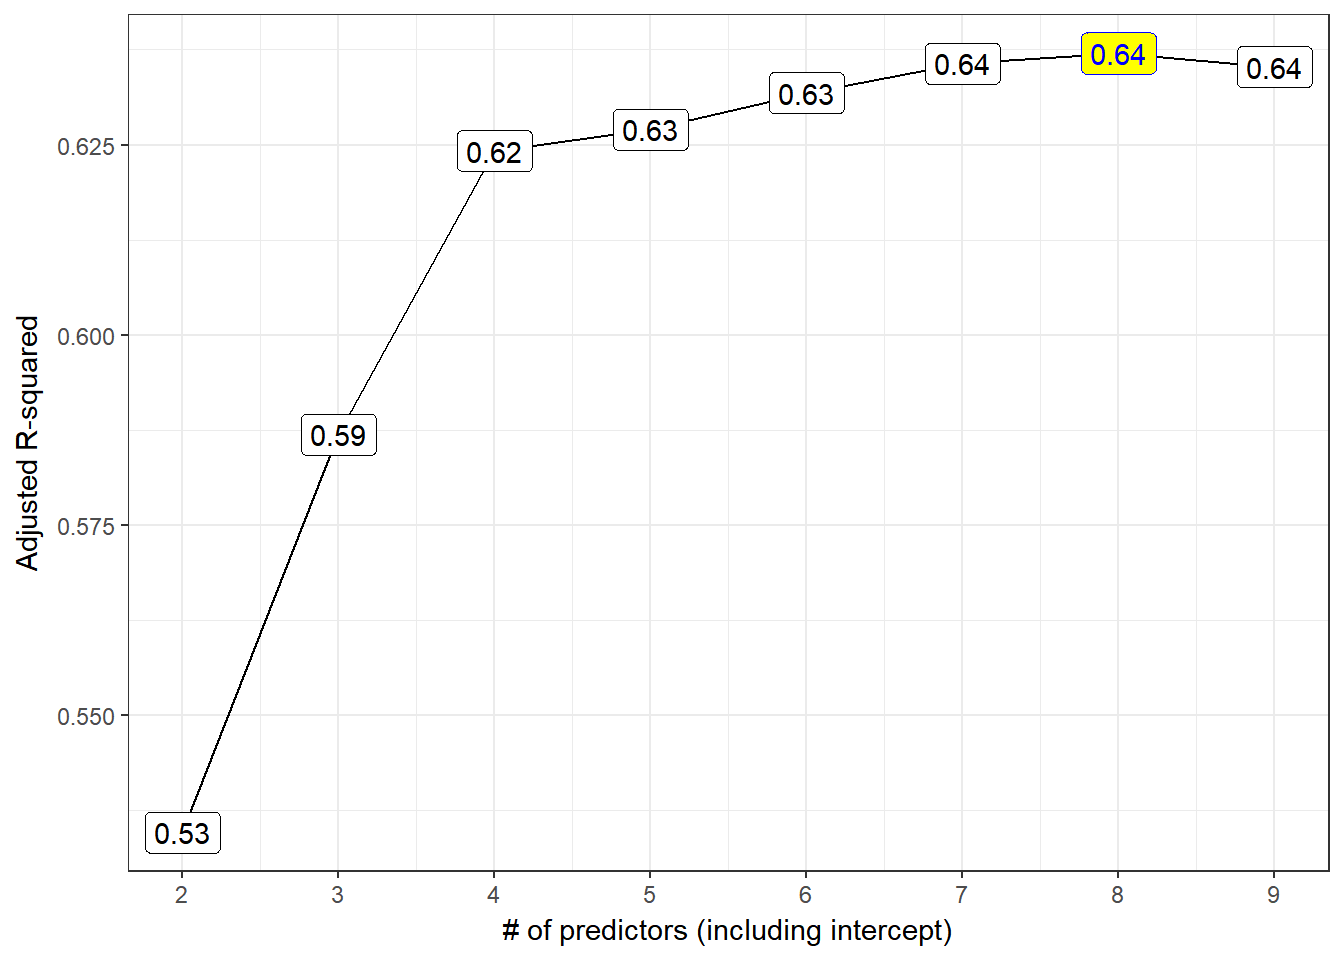
\includegraphics{bookdown-demo_files/figure-latex/unnamed-chunk-77-1.pdf}

Models 4-9 all look like reasonable choices here. The maximum adjusted
R\textsuperscript{2} is seen in the model of size 8.

\subsection{\texorpdfstring{Mallows'
\(C_p\)}{Mallows' C\_p}}\label{mallows-c_p}

The \(C_p\) statistic focuses directly on the tradeoff between
\textbf{bias} (due to excluding important predictors from the model) and
extra \textbf{variance} (due to including too many unimportant
predictors in the model.)

If N is the sample size, and we select \(p\) regression predictors from
a set of \(K\) (where \(p < K\)), then the \(C_p\) statistic is

\(C_p = \frac{SSE_p}{MSE_K} - N + 2p\)

where:

\begin{itemize}
\tightlist
\item
  \(SSE_p\) is the sum of squares for error (residual) in the model with
  \(p\) predictors
\item
  \(MSE_K\) is the residual mean square after regression in the model
  with all \(K\) predictors
\end{itemize}

As it turns out, this is just measuring the particular model's lack of
fit, and then adding a penalty for the number of terms in the model
(specifically \(2p - N\) is the penalty since the lack of fit is
measured as \((N-p) \frac{SSE_p}{MSE_K}\).

\begin{itemize}
\tightlist
\item
  If a model has no meaningful lack of fit (i.e.~no substantial bias)
  then the expected value of \(C_p\) is roughly \(p\).
\item
  Otherwise, the expectation is \(p\) plus a positive bias term.
\item
  In general, we want to see \emph{smaller} values of \(C_p\).
\item
  We usually select a ``winning model'' by choosing a subset of
  predictors that have \(C_p\) near the value of \(p\).
\end{itemize}

\subsection{\texorpdfstring{The \(C_p\)
Plot}{The C\_p Plot}}\label{the-c_p-plot}

The \(C_p\) plot is just a scatterplot of \(C_p\) on the Y-axis, and the
size of the model (coefficients plus intercept) \(p = k\) on the X-axis.

Each of the various predictor subsets we will study is represented in a
single point. A model without bias should have \(C_p\) roughly equal to
\(p\), so we'll frequently draw a line at \(C_p = p\) to make that
clear. We then select our model from among all models with small \(C_p\)
statistics.

\begin{itemize}
\tightlist
\item
  My typical approach is to identify the models where
  \(C_p - p \geq 0\), then select from among those models the model
  where \(C_p - p\) is minimized, and if there is a tie, select the
  model where \(p\) is minimized.
\item
  Another good candidate might be a slightly overfit model (where
  \(C_p - p < 0\) but just barely.)
\end{itemize}

\begin{Shaded}
\begin{Highlighting}[]
\NormalTok{p2 <-}\StringTok{ }\KeywordTok{ggplot}\NormalTok{(best_mods, }\KeywordTok{aes}\NormalTok{(}\DataTypeTok{x =}\NormalTok{ k, }\DataTypeTok{y =}\NormalTok{ cp,}
                            \DataTypeTok{label =} \KeywordTok{round}\NormalTok{(cp,}\DecValTok{1}\NormalTok{))) }\OperatorTok{+}
\StringTok{    }\KeywordTok{geom_line}\NormalTok{() }\OperatorTok{+}
\StringTok{    }\KeywordTok{geom_label}\NormalTok{() }\OperatorTok{+}
\StringTok{    }\KeywordTok{geom_abline}\NormalTok{(}\DataTypeTok{intercept =} \DecValTok{0}\NormalTok{, }\DataTypeTok{slope =} \DecValTok{1}\NormalTok{,}
                \DataTypeTok{col =} \StringTok{"red"}\NormalTok{) }\OperatorTok{+}
\StringTok{    }\KeywordTok{theme_bw}\NormalTok{() }\OperatorTok{+}
\StringTok{    }\KeywordTok{scale_x_continuous}\NormalTok{(}\DataTypeTok{breaks =} \DecValTok{2}\OperatorTok{:}\DecValTok{9}\NormalTok{) }\OperatorTok{+}
\StringTok{    }\KeywordTok{labs}\NormalTok{(}\DataTypeTok{x =} \StringTok{"# of predictors (including intercept)"}\NormalTok{,}
         \DataTypeTok{y =} \StringTok{"Mallows' Cp"}\NormalTok{)}

\NormalTok{p2}
\end{Highlighting}
\end{Shaded}

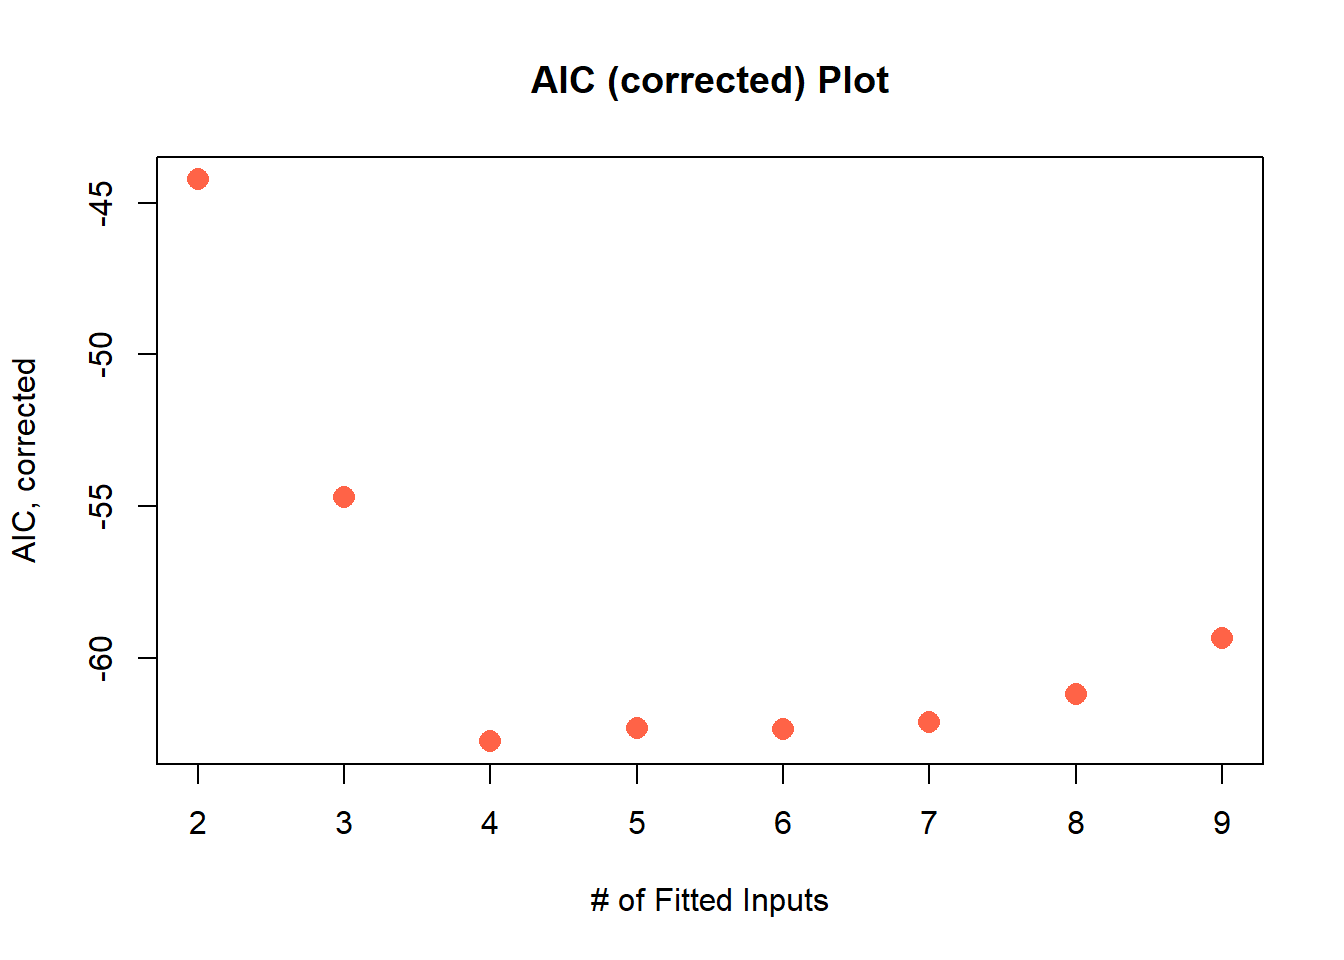
\includegraphics{bookdown-demo_files/figure-latex/unnamed-chunk-78-1.pdf}

\begin{itemize}
\tightlist
\item
  Model 6 is a possibility here, with the difference \(C_p - p\)
  minimized among all models with \(C_p >= p\).
\item
  Model 7 also looks pretty good, with C\textsubscript{p} just barely
  smaller than the size (p = 7) of the model.
\end{itemize}

\subsection{\texorpdfstring{``All Subsets'' Regression and Information
Criteria}{All Subsets Regression and Information Criteria}}\label{all-subsets-regression-and-information-criteria}

We might consider any of three main information criteria:

\begin{itemize}
\tightlist
\item
  the Bayesian Information Criterion, called BIC
\item
  the Akaike Information Criterion (used by R's default stepwise
  approaches,) called AIC
\item
  a corrected version of AIC due to \citet{HurvichTsai1989}, called
  AIC\textsubscript{c} or \texttt{aic.c}
\end{itemize}

Each of these indicates better models by getting smaller. Since the
\(C_p\) and AIC results will lead to the same model, I'll focus on
plotting the bias-corrected AIC and on BIC.

\subsection{The bias-corrected AIC
plot}\label{the-bias-corrected-aic-plot}

\begin{Shaded}
\begin{Highlighting}[]
\NormalTok{p3 <-}\StringTok{ }\KeywordTok{ggplot}\NormalTok{(best_mods, }\KeywordTok{aes}\NormalTok{(}\DataTypeTok{x =}\NormalTok{ k, }\DataTypeTok{y =}\NormalTok{ aic.c,}
                             \DataTypeTok{label =} \KeywordTok{round}\NormalTok{(aic.c,}\DecValTok{1}\NormalTok{))) }\OperatorTok{+}
\StringTok{    }\KeywordTok{geom_line}\NormalTok{() }\OperatorTok{+}
\StringTok{    }\KeywordTok{geom_label}\NormalTok{() }\OperatorTok{+}
\StringTok{    }\KeywordTok{geom_label}\NormalTok{(}\DataTypeTok{data =} \KeywordTok{subset}\NormalTok{(best_mods, aic.c }\OperatorTok{==}\StringTok{ }\KeywordTok{min}\NormalTok{(aic.c)),}
               \KeywordTok{aes}\NormalTok{(}\DataTypeTok{x =}\NormalTok{ k, }\DataTypeTok{y =}\NormalTok{ aic.c), }\DataTypeTok{fill =} \StringTok{"pink"}\NormalTok{, }
               \DataTypeTok{col =} \StringTok{"red"}\NormalTok{) }\OperatorTok{+}
\StringTok{    }\KeywordTok{theme_bw}\NormalTok{() }\OperatorTok{+}
\StringTok{    }\KeywordTok{scale_x_continuous}\NormalTok{(}\DataTypeTok{breaks =} \DecValTok{2}\OperatorTok{:}\DecValTok{9}\NormalTok{) }\OperatorTok{+}
\StringTok{    }\KeywordTok{labs}\NormalTok{(}\DataTypeTok{x =} \StringTok{"# of predictors (including intercept)"}\NormalTok{,}
         \DataTypeTok{y =} \StringTok{"Bias-Corrected AIC"}\NormalTok{)}

\NormalTok{p3}
\end{Highlighting}
\end{Shaded}

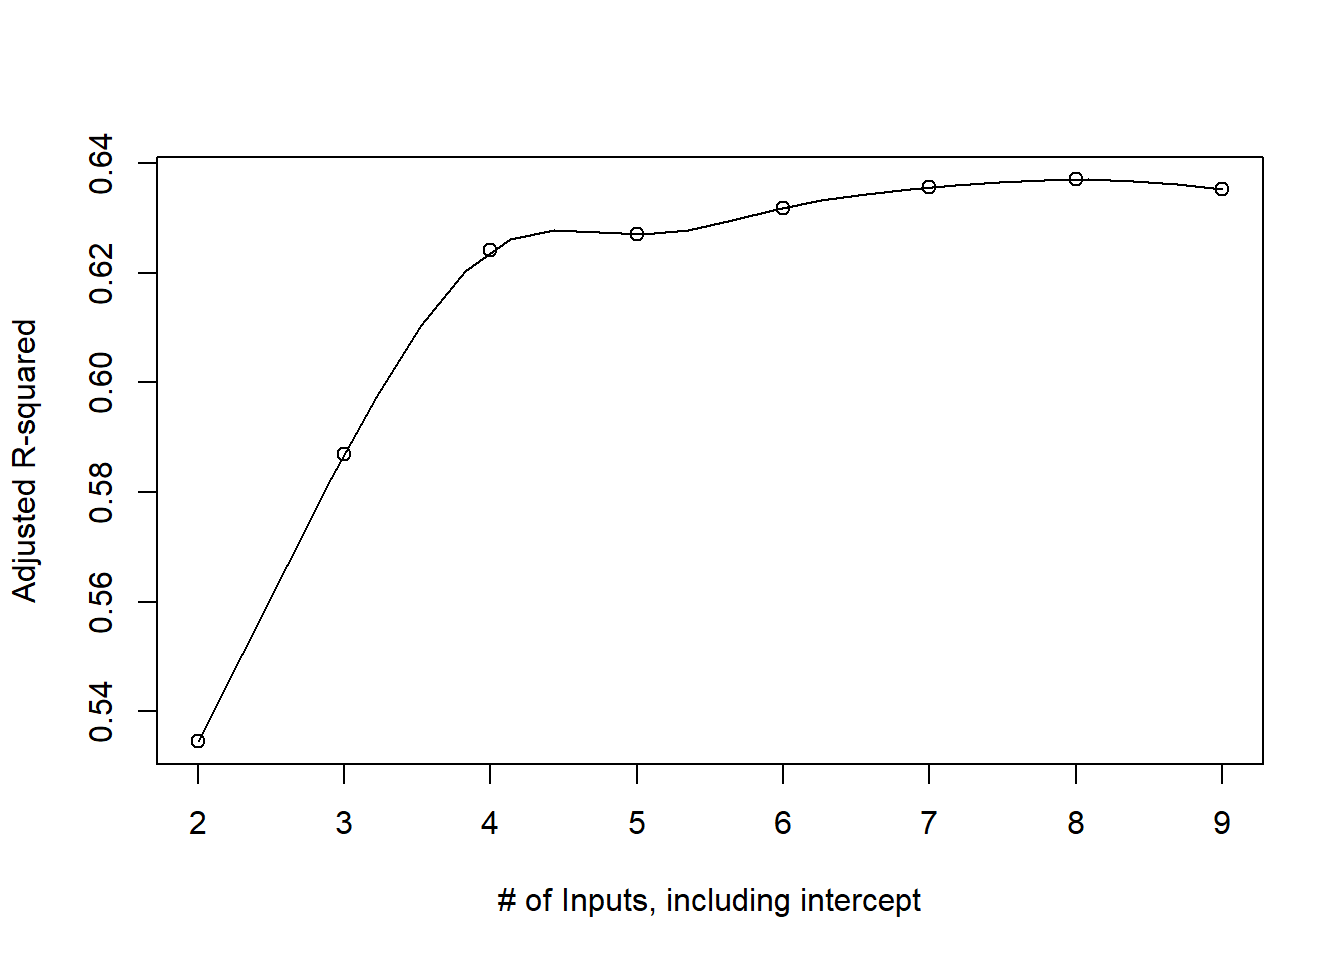
\includegraphics{bookdown-demo_files/figure-latex/unnamed-chunk-79-1.pdf}

The smallest AIC\textsubscript{c} values occur in models 4 and later,
especially model 4 itself.

\subsection{The BIC plot}\label{the-bic-plot}

\begin{Shaded}
\begin{Highlighting}[]
\NormalTok{p4 <-}\StringTok{ }\KeywordTok{ggplot}\NormalTok{(best_mods, }\KeywordTok{aes}\NormalTok{(}\DataTypeTok{x =}\NormalTok{ k, }\DataTypeTok{y =}\NormalTok{ bic,}
                            \DataTypeTok{label =} \KeywordTok{round}\NormalTok{(bic,}\DecValTok{1}\NormalTok{))) }\OperatorTok{+}
\StringTok{    }\KeywordTok{geom_line}\NormalTok{() }\OperatorTok{+}
\StringTok{    }\KeywordTok{geom_label}\NormalTok{() }\OperatorTok{+}
\StringTok{    }\KeywordTok{geom_label}\NormalTok{(}\DataTypeTok{data =} \KeywordTok{subset}\NormalTok{(best_mods, bic }\OperatorTok{==}\StringTok{ }\KeywordTok{min}\NormalTok{(bic)),}
               \KeywordTok{aes}\NormalTok{(}\DataTypeTok{x =}\NormalTok{ k, }\DataTypeTok{y =}\NormalTok{ bic),}
               \DataTypeTok{fill =} \StringTok{"lightgreen"}\NormalTok{, }\DataTypeTok{col =} \StringTok{"blue"}\NormalTok{) }\OperatorTok{+}
\StringTok{    }\KeywordTok{theme_bw}\NormalTok{() }\OperatorTok{+}
\StringTok{    }\KeywordTok{scale_x_continuous}\NormalTok{(}\DataTypeTok{breaks =} \DecValTok{2}\OperatorTok{:}\DecValTok{9}\NormalTok{) }\OperatorTok{+}
\StringTok{    }\KeywordTok{labs}\NormalTok{(}\DataTypeTok{x =} \StringTok{"# of predictors (including intercept)"}\NormalTok{,}
         \DataTypeTok{y =} \StringTok{"BIC"}\NormalTok{)}

\NormalTok{p4}
\end{Highlighting}
\end{Shaded}

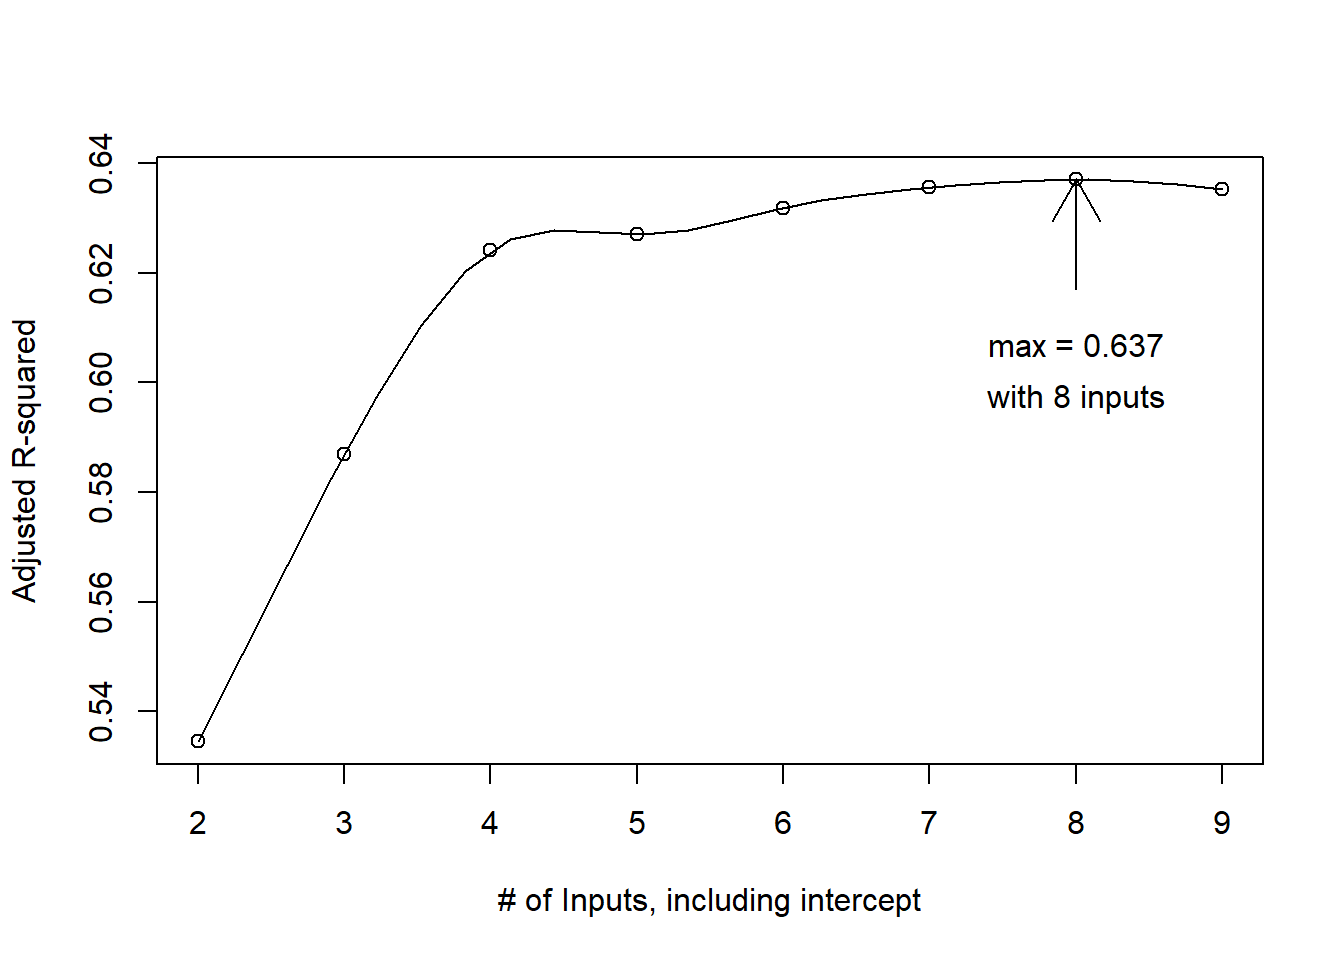
\includegraphics{bookdown-demo_files/figure-latex/unnamed-chunk-80-1.pdf}

\subsection{All Four Plots in One Figure (via
ggplot2)}\label{all-four-plots-in-one-figure-via-ggplot2}

\begin{Shaded}
\begin{Highlighting}[]
\NormalTok{gridExtra}\OperatorTok{::}\KeywordTok{grid.arrange}\NormalTok{(p1, p2, p3, p4, }\DataTypeTok{nrow =} \DecValTok{2}\NormalTok{)}
\end{Highlighting}
\end{Shaded}

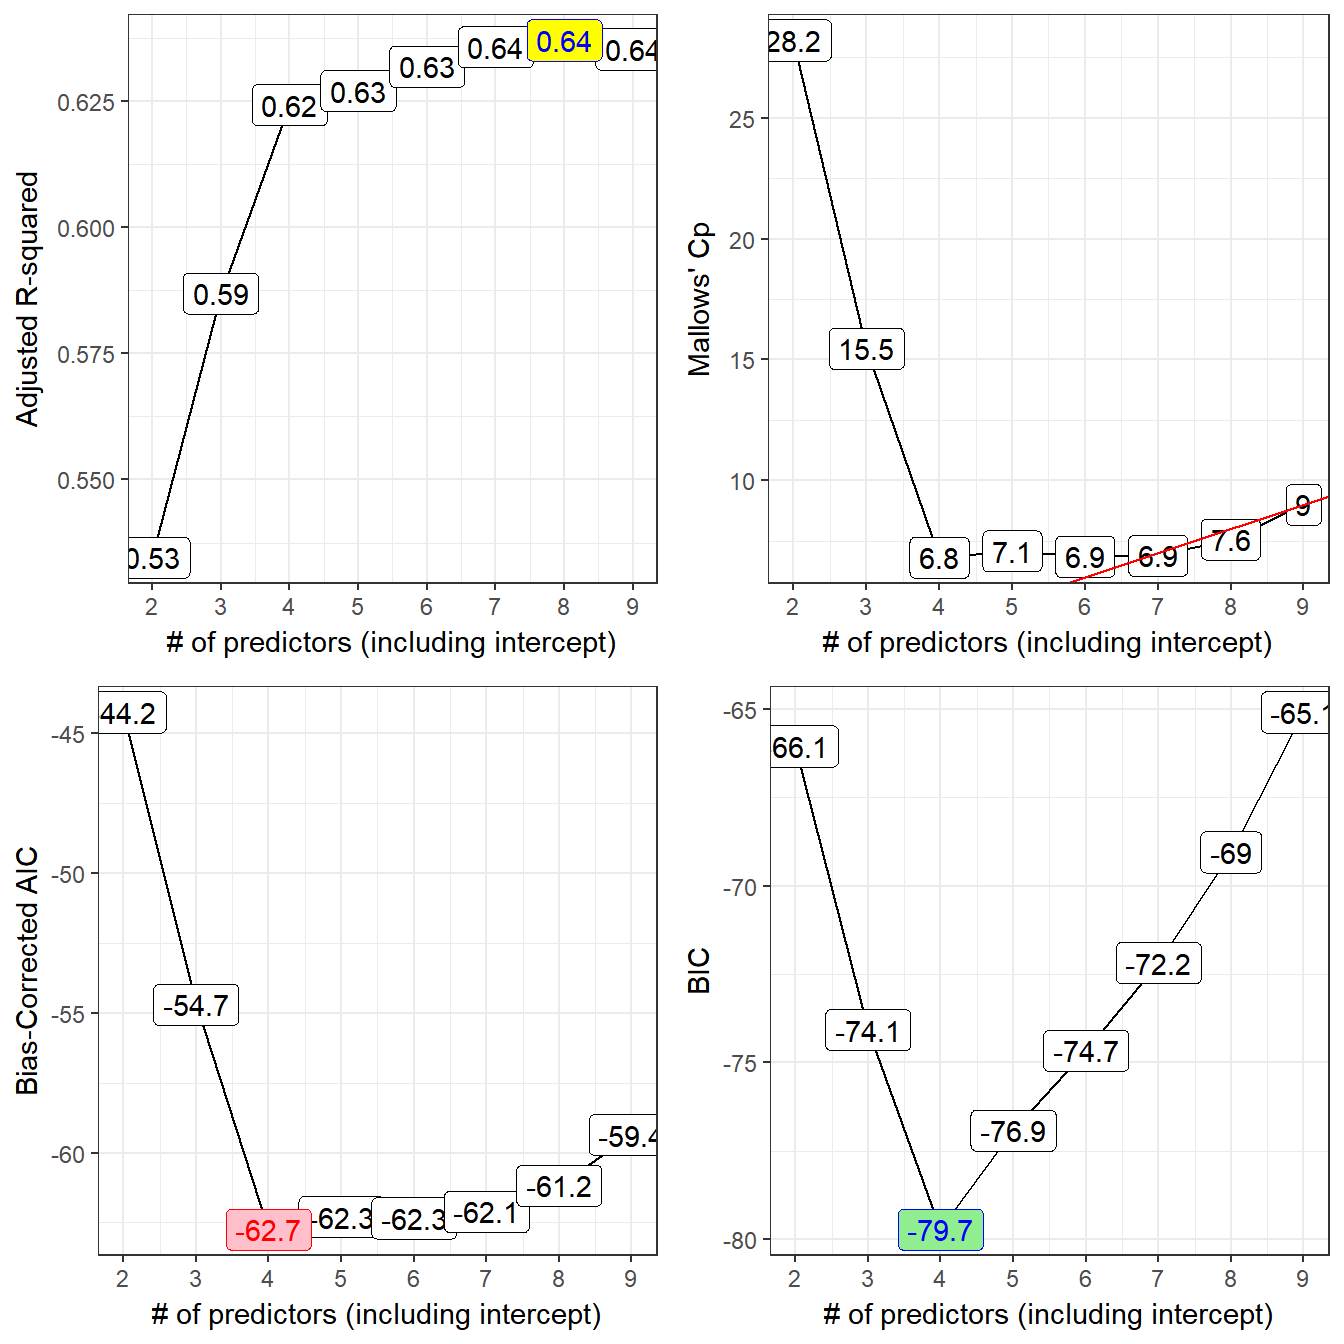
\includegraphics{bookdown-demo_files/figure-latex/unnamed-chunk-81-1.pdf}

\section{Table of Key Results}\label{table-of-key-results}

We can build a big table, like this:

\begin{Shaded}
\begin{Highlighting}[]
\NormalTok{best_mods}
\end{Highlighting}
\end{Shaded}

\begin{verbatim}
  k        r2     adjr2        cp     aic.c       bic (Intercept) lcavol
1 2 0.5394320 0.5345839 28.213914 -44.23838 -66.05416        TRUE   TRUE
2 3 0.5955040 0.5868977 15.456669 -54.70040 -74.07188        TRUE   TRUE
3 4 0.6359499 0.6242063  6.811986 -62.74265 -79.71614        TRUE   TRUE
4 5 0.6425479 0.6270065  7.075509 -62.29223 -76.91557        TRUE   TRUE
5 6 0.6509970 0.6318211  6.851826 -62.33858 -74.66120        TRUE   TRUE
6 7 0.6584484 0.6356783  6.890739 -62.10692 -72.17992        TRUE   TRUE
7 8 0.6634967 0.6370302  7.562119 -61.17338 -69.04961        TRUE   TRUE
8 9 0.6656326 0.6352355  9.000000 -59.35841 -65.09253        TRUE   TRUE
  lweight   age bph_f svi_f   lcp gleason_f pgg45
1   FALSE FALSE FALSE FALSE FALSE     FALSE FALSE
2    TRUE FALSE FALSE FALSE FALSE     FALSE FALSE
3    TRUE FALSE FALSE  TRUE FALSE     FALSE FALSE
4    TRUE FALSE  TRUE  TRUE FALSE     FALSE FALSE
5    TRUE  TRUE  TRUE  TRUE FALSE     FALSE FALSE
6    TRUE  TRUE  TRUE  TRUE FALSE      TRUE FALSE
7    TRUE  TRUE  TRUE  TRUE  TRUE      TRUE FALSE
8    TRUE  TRUE  TRUE  TRUE  TRUE      TRUE  TRUE
\end{verbatim}

\section{Models Worth Considering?}\label{models-worth-considering}

\begin{longtable}[]{@{}rrll@{}}
\toprule
\(k\) & Predictors & Reason\tabularnewline
\midrule
\endhead
4 & \texttt{lcavol\ lweight\ svi\_f} & minimizes BIC,
AIC\textsubscript{c}\tabularnewline
7 & \texttt{+\ age\ bph\_f\ gleason\_f} & \(C_p\) near
\emph{p}\tabularnewline
8 & \texttt{+\ lcp} & max \(R^2_{adj}\)\tabularnewline
\bottomrule
\end{longtable}

\section{Compare these candidate models
in-sample?}\label{compare-these-candidate-models-in-sample}

\subsection{\texorpdfstring{Using \texttt{anova} to compare nested
models}{Using anova to compare nested models}}\label{using-anova-to-compare-nested-models}

Let's run an ANOVA-based comparison of these nested models to each other
and to the model with the intercept alone.

\begin{itemize}
\tightlist
\item
  The models are \textbf{nested} because \texttt{m04} is a subset of the
  predictors in \texttt{m07}, which includes a subset of the predictors
  in \texttt{m08}.
\end{itemize}

\begin{Shaded}
\begin{Highlighting}[]
\NormalTok{m.int <-}\StringTok{ }\KeywordTok{lm}\NormalTok{(lpsa }\OperatorTok{~}\StringTok{ }\DecValTok{1}\NormalTok{, }\DataTypeTok{data =}\NormalTok{ prost)}
\NormalTok{m04 <-}\StringTok{ }\KeywordTok{lm}\NormalTok{(lpsa }\OperatorTok{~}\StringTok{ }\NormalTok{lcavol }\OperatorTok{+}\StringTok{ }\NormalTok{lweight }\OperatorTok{+}\StringTok{ }\NormalTok{svi_f, }\DataTypeTok{data =}\NormalTok{ prost)}
\NormalTok{m07 <-}\StringTok{ }\KeywordTok{lm}\NormalTok{(lpsa }\OperatorTok{~}\StringTok{ }\NormalTok{lcavol }\OperatorTok{+}\StringTok{ }\NormalTok{lweight }\OperatorTok{+}\StringTok{ }\NormalTok{svi_f }\OperatorTok{+}\StringTok{ }
\StringTok{              }\NormalTok{age }\OperatorTok{+}\StringTok{ }\NormalTok{bph_f }\OperatorTok{+}\StringTok{ }\NormalTok{gleason_f, }\DataTypeTok{data =}\NormalTok{ prost)}
\NormalTok{m08 <-}\StringTok{ }\KeywordTok{lm}\NormalTok{(lpsa }\OperatorTok{~}\StringTok{ }\NormalTok{lcavol }\OperatorTok{+}\StringTok{ }\NormalTok{lweight }\OperatorTok{+}\StringTok{ }\NormalTok{svi_f }\OperatorTok{+}\StringTok{ }
\StringTok{              }\NormalTok{age }\OperatorTok{+}\StringTok{ }\NormalTok{bph_f }\OperatorTok{+}\StringTok{ }\NormalTok{gleason_f }\OperatorTok{+}\StringTok{ }\NormalTok{lcp, }\DataTypeTok{data =}\NormalTok{ prost)}
\NormalTok{m.full <-}\StringTok{ }\KeywordTok{lm}\NormalTok{(lpsa }\OperatorTok{~}\StringTok{ }\NormalTok{lcavol }\OperatorTok{+}\StringTok{ }\NormalTok{lweight }\OperatorTok{+}\StringTok{ }\NormalTok{svi_f }\OperatorTok{+}\StringTok{ }
\StringTok{              }\NormalTok{age }\OperatorTok{+}\StringTok{ }\NormalTok{bph_f }\OperatorTok{+}\StringTok{ }\NormalTok{gleason_f }\OperatorTok{+}\StringTok{ }\NormalTok{lcp }\OperatorTok{+}\StringTok{ }\NormalTok{pgg45, }\DataTypeTok{data =}\NormalTok{ prost)}
\end{Highlighting}
\end{Shaded}

Next, we'll run\ldots{}

\begin{Shaded}
\begin{Highlighting}[]
\KeywordTok{anova}\NormalTok{(m.full, m08, m07, m04, m.int)}
\end{Highlighting}
\end{Shaded}

\begin{verbatim}
Analysis of Variance Table

Model 1: lpsa ~ lcavol + lweight + svi_f + age + bph_f + gleason_f + lcp + 
    pgg45
Model 2: lpsa ~ lcavol + lweight + svi_f + age + bph_f + gleason_f + lcp
Model 3: lpsa ~ lcavol + lweight + svi_f + age + bph_f + gleason_f
Model 4: lpsa ~ lcavol + lweight + svi_f
Model 5: lpsa ~ 1
  Res.Df     RSS Df Sum of Sq       F Pr(>F)    
1     86  41.057                                
2     87  41.498 -1    -0.441  0.9234 0.3393    
3     88  42.066 -1    -0.568  1.1891 0.2786    
4     93  46.568 -5    -4.503  1.8863 0.1050    
5     96 127.918 -3   -81.349 56.7991 <2e-16 ***
---
Signif. codes:  0 '***' 0.001 '**' 0.01 '*' 0.05 '.' 0.1 ' ' 1
\end{verbatim}

What conclusions can we draw here, on the basis of these ANOVA tests?

\begin{itemize}
\tightlist
\item
  The first \emph{p} value, of 0.3393, compares what the \texttt{anova}
  called Model 1, and what we call \texttt{m.full} to what the
  \texttt{anova} called Model 2, and what we call \texttt{m08}. So
  there's no significant decline in predictive value observed when we
  drop from the \texttt{m.full} model to the \texttt{m08} model. This
  suggests that the \texttt{m08} model may be a better choice.
\item
  The second \emph{p} value, of 0.2786, compares \texttt{m08} to
  \texttt{m07}, and suggests that we lose no significant predictive
  value by dropping down to \texttt{m07}.
\item
  The third \emph{p} value, of 0.1050, compares \texttt{m07} to
  \texttt{m04}, and suggests that we lose no significant predictive
  value by dropping down to \texttt{m04}.
\item
  But the fourth \emph{p} value, of 2e-16 (or, functionally, zero),
  compares \texttt{m04} to \texttt{m.int} and suggests that we do gain
  significant predictive value by including the predictors in
  \texttt{m04} as compared to a model with an intercept alone.
\item
  So, by the significance tests, the model we'd select would be
  \texttt{m04}, but, of course, in-sample statistical significance alone
  isn't a good enough reason to select a model if we want to do
  prediction well.
\end{itemize}

\section{AIC and BIC comparisons, within the training
sample}\label{aic-and-bic-comparisons-within-the-training-sample}

Next, we'll compare the three candidate models (ignoring the
intercept-only and kitchen sink models) in terms of their AIC values and
BIC values, again using the same sample we used to fit the models in the
first place.

\begin{Shaded}
\begin{Highlighting}[]
\KeywordTok{AIC}\NormalTok{(m04, m07, m08)}
\end{Highlighting}
\end{Shaded}

\begin{verbatim}
    df      AIC
m04  5 214.0966
m07 10 214.2327
m08 11 214.9148
\end{verbatim}

\begin{Shaded}
\begin{Highlighting}[]
\KeywordTok{BIC}\NormalTok{(m04, m07, m08)}
\end{Highlighting}
\end{Shaded}

\begin{verbatim}
    df      BIC
m04  5 226.9702
m07 10 239.9798
m08 11 243.2366
\end{verbatim}

\begin{itemize}
\tightlist
\item
  The model with the smallest AIC value shows the best performance
  within the sample on that measure.
\item
  Similarly, smaller BIC values are associated with predictor sets that
  perform better in sample on that criterion.
\item
  BIC often suggests smaller models (with fewer regression inputs) than
  does AIC. Does that happen in this case?
\item
  Note that \texttt{AIC} and \texttt{BIC} can be calculated in a few
  different ways, so we may see some variation if we don't compare
  apples to apples with regard to the R functions involved.
\end{itemize}

\section{Cross-Validation of Candidate Models out of
Sample}\label{cross-validation-of-candidate-models-out-of-sample}

\subsection{\texorpdfstring{20-fold Cross-Validation of model
\texttt{m04}}{20-fold Cross-Validation of model m04}}\label{fold-cross-validation-of-model-m04}

Model \texttt{m04} uses \texttt{lcavol}, \texttt{lweight} and
\texttt{svi\_f} to predict the \texttt{lpsa} outcome. Let's do 20-fold
cross-validation of this modeling approach, and calculate the root mean
squared prediction error and the mean absolute prediction error for that
modeling scheme.

\begin{Shaded}
\begin{Highlighting}[]
\KeywordTok{set.seed}\NormalTok{(}\DecValTok{43201}\NormalTok{)}

\NormalTok{cv_m04 <-}\StringTok{ }\NormalTok{prost }\OperatorTok
\StringTok{    }\KeywordTok{crossv_kfold}\NormalTok{(}\DataTypeTok{k =} \DecValTok{20}\NormalTok{) }\OperatorTok
\StringTok{    }\KeywordTok{mutate}\NormalTok{(}\DataTypeTok{model =} \KeywordTok{map}\NormalTok{(train, }
                       \OperatorTok{~}\StringTok{ }\KeywordTok{lm}\NormalTok{(lpsa }\OperatorTok{~}\StringTok{ }\NormalTok{lcavol }\OperatorTok{+}\StringTok{ }\NormalTok{lweight }\OperatorTok{+}\StringTok{ }\NormalTok{svi_f,}
                                   \DataTypeTok{data =}\NormalTok{ .)))}

\NormalTok{cv_m04_pred <-}\StringTok{ }\NormalTok{cv_m04 }\OperatorTok
\StringTok{    }\KeywordTok{unnest}\NormalTok{(}\KeywordTok{map2}\NormalTok{(model, test, }\OperatorTok{~}\StringTok{ }\KeywordTok{augment}\NormalTok{(.x, }\DataTypeTok{newdata =}\NormalTok{ .y)))}

\NormalTok{cv_m04_results <-}\StringTok{ }\NormalTok{cv_m04_pred }\OperatorTok
\StringTok{    }\KeywordTok{summarize}\NormalTok{(}\DataTypeTok{Model =} \StringTok{"m04"}\NormalTok{, }
              \DataTypeTok{RMSE =} \KeywordTok{sqrt}\NormalTok{(}\KeywordTok{mean}\NormalTok{((lpsa }\OperatorTok{-}\StringTok{ }\NormalTok{.fitted) }\OperatorTok{^}\DecValTok{2}\NormalTok{)),}
              \DataTypeTok{MAE =} \KeywordTok{mean}\NormalTok{(}\KeywordTok{abs}\NormalTok{(lpsa }\OperatorTok{-}\StringTok{ }\NormalTok{.fitted)))}

\NormalTok{cv_m04_results}
\end{Highlighting}
\end{Shaded}

\begin{verbatim}
# A tibble: 1 x 3
  Model  RMSE   MAE
  <chr> <dbl> <dbl>
1 m04   0.725 0.574
\end{verbatim}

\subsection{\texorpdfstring{20-fold Cross-Validation of model
\texttt{m07}}{20-fold Cross-Validation of model m07}}\label{fold-cross-validation-of-model-m07}

Model \texttt{m07} uses \texttt{lcavol}, \texttt{lweight},
\texttt{svi\_f}, \texttt{age}, \texttt{bph\_f}, and \texttt{gleason\_f}
to predict the \texttt{lpsa} outcome. Let's now do 20-fold
cross-validation of this modeling approach, and calculate the root mean
squared prediction error and the mean absolute prediction error for that
modeling scheme. Note the small changes required, as compared to our
cross-validation of model \texttt{m04} a moment ago.

\begin{Shaded}
\begin{Highlighting}[]
\KeywordTok{set.seed}\NormalTok{(}\DecValTok{43202}\NormalTok{)}

\NormalTok{cv_m07 <-}\StringTok{ }\NormalTok{prost }\OperatorTok
\StringTok{    }\KeywordTok{crossv_kfold}\NormalTok{(}\DataTypeTok{k =} \DecValTok{20}\NormalTok{) }\OperatorTok
\StringTok{    }\KeywordTok{mutate}\NormalTok{(}\DataTypeTok{model =} \KeywordTok{map}\NormalTok{(train, }
                       \OperatorTok{~}\StringTok{ }\KeywordTok{lm}\NormalTok{(lpsa }\OperatorTok{~}\StringTok{ }\NormalTok{lcavol }\OperatorTok{+}\StringTok{ }\NormalTok{lweight }\OperatorTok{+}\StringTok{ }
\StringTok{                                }\NormalTok{svi_f }\OperatorTok{+}\StringTok{ }\NormalTok{age }\OperatorTok{+}\StringTok{ }\NormalTok{bph_f }\OperatorTok{+}\StringTok{ }
\StringTok{                                }\NormalTok{gleason_f,}
                                   \DataTypeTok{data =}\NormalTok{ .)))}

\NormalTok{cv_m07_pred <-}\StringTok{ }\NormalTok{cv_m07 }\OperatorTok
\StringTok{    }\KeywordTok{unnest}\NormalTok{(}\KeywordTok{map2}\NormalTok{(model, test, }\OperatorTok{~}\StringTok{ }\KeywordTok{augment}\NormalTok{(.x, }\DataTypeTok{newdata =}\NormalTok{ .y)))}

\NormalTok{cv_m07_results <-}\StringTok{ }\NormalTok{cv_m07_pred }\OperatorTok
\StringTok{    }\KeywordTok{summarize}\NormalTok{(}\DataTypeTok{Model =} \StringTok{"m07"}\NormalTok{, }
              \DataTypeTok{RMSE =} \KeywordTok{sqrt}\NormalTok{(}\KeywordTok{mean}\NormalTok{((lpsa }\OperatorTok{-}\StringTok{ }\NormalTok{.fitted) }\OperatorTok{^}\DecValTok{2}\NormalTok{)),}
              \DataTypeTok{MAE =} \KeywordTok{mean}\NormalTok{(}\KeywordTok{abs}\NormalTok{(lpsa }\OperatorTok{-}\StringTok{ }\NormalTok{.fitted)))}

\NormalTok{cv_m07_results}
\end{Highlighting}
\end{Shaded}

\begin{verbatim}
# A tibble: 1 x 3
  Model  RMSE   MAE
  <chr> <dbl> <dbl>
1 m07   0.730 0.556
\end{verbatim}

\subsection{\texorpdfstring{20-fold Cross-Validation of model
\texttt{m08}}{20-fold Cross-Validation of model m08}}\label{fold-cross-validation-of-model-m08}

Model \texttt{m08} uses \texttt{lcavol}, \texttt{lweight},
\texttt{svi\_f}, \texttt{age}, \texttt{bph\_f}, \texttt{gleason\_f} and
\texttt{lcp} to predict the \texttt{lpsa} outcome. Let's now do 20-fold
cross-validation of this modeling approach.

\begin{Shaded}
\begin{Highlighting}[]
\KeywordTok{set.seed}\NormalTok{(}\DecValTok{43202}\NormalTok{)}

\NormalTok{cv_m08 <-}\StringTok{ }\NormalTok{prost }\OperatorTok
\StringTok{    }\KeywordTok{crossv_kfold}\NormalTok{(}\DataTypeTok{k =} \DecValTok{20}\NormalTok{) }\OperatorTok
\StringTok{    }\KeywordTok{mutate}\NormalTok{(}\DataTypeTok{model =} \KeywordTok{map}\NormalTok{(train, }
                       \OperatorTok{~}\StringTok{ }\KeywordTok{lm}\NormalTok{(lpsa }\OperatorTok{~}\StringTok{ }\NormalTok{lcavol }\OperatorTok{+}\StringTok{ }\NormalTok{lweight }\OperatorTok{+}\StringTok{ }
\StringTok{                                }\NormalTok{svi_f }\OperatorTok{+}\StringTok{ }\NormalTok{age }\OperatorTok{+}\StringTok{ }\NormalTok{bph_f }\OperatorTok{+}\StringTok{ }
\StringTok{                                }\NormalTok{gleason_f }\OperatorTok{+}\StringTok{ }\NormalTok{lcp,}
                                   \DataTypeTok{data =}\NormalTok{ .)))}

\NormalTok{cv_m08_pred <-}\StringTok{ }\NormalTok{cv_m08 }\OperatorTok
\StringTok{    }\KeywordTok{unnest}\NormalTok{(}\KeywordTok{map2}\NormalTok{(model, test, }\OperatorTok{~}\StringTok{ }\KeywordTok{augment}\NormalTok{(.x, }\DataTypeTok{newdata =}\NormalTok{ .y)))}

\NormalTok{cv_m08_results <-}\StringTok{ }\NormalTok{cv_m08_pred }\OperatorTok
\StringTok{    }\KeywordTok{summarize}\NormalTok{(}\DataTypeTok{Model =} \StringTok{"m08"}\NormalTok{, }
              \DataTypeTok{RMSE =} \KeywordTok{sqrt}\NormalTok{(}\KeywordTok{mean}\NormalTok{((lpsa }\OperatorTok{-}\StringTok{ }\NormalTok{.fitted) }\OperatorTok{^}\DecValTok{2}\NormalTok{)),}
              \DataTypeTok{MAE =} \KeywordTok{mean}\NormalTok{(}\KeywordTok{abs}\NormalTok{(lpsa }\OperatorTok{-}\StringTok{ }\NormalTok{.fitted)))}

\NormalTok{cv_m08_results}
\end{Highlighting}
\end{Shaded}

\begin{verbatim}
# A tibble: 1 x 3
  Model  RMSE   MAE
  <chr> <dbl> <dbl>
1 m08   0.729 0.557
\end{verbatim}

\subsection{Comparing the Results of the
Cross-Validations}\label{comparing-the-results-of-the-cross-validations}

\begin{Shaded}
\begin{Highlighting}[]
\KeywordTok{bind_rows}\NormalTok{(cv_m04_results, cv_m07_results, cv_m08_results)}
\end{Highlighting}
\end{Shaded}

\begin{verbatim}
# A tibble: 3 x 3
  Model  RMSE   MAE
  <chr> <dbl> <dbl>
1 m04   0.725 0.574
2 m07   0.730 0.556
3 m08   0.729 0.557
\end{verbatim}

It appears that model \texttt{m04} has the smallest RMSE and MAE in this
case. So, that's the model with the strongest cross-validated predictive
accuracy, by these two standards.

\section{What about Interaction
Terms?}\label{what-about-interaction-terms}

Suppose we consider for a moment a much smaller and less realistic
problem. We want to use best subsets to identify a model out of a set of
three predictors for \texttt{lpsa}: specifically \texttt{lcavol},
\texttt{age} and \texttt{svi\_f}, but now we also want to consider the
interaction of \texttt{svi\_f} with \texttt{lcavol} as a potential
addition. Remember that \texttt{svi} is the 1/0 numeric version of
\texttt{svi\_f}. We could simply add a numerical product term to our
model, as follows.

\begin{Shaded}
\begin{Highlighting}[]
\NormalTok{pred2 <-}\StringTok{ }\KeywordTok{with}\NormalTok{(prost, }\KeywordTok{cbind}\NormalTok{(lcavol, age, svi_f, }\DataTypeTok{svixlcavol =}\NormalTok{ svi}\OperatorTok{*}\NormalTok{lcavol))}

\NormalTok{rs.ks2 <-}\StringTok{ }\KeywordTok{regsubsets}\NormalTok{(pred2, }\DataTypeTok{y =}\NormalTok{ prost}\OperatorTok{$}\NormalTok{lpsa, }
                    \DataTypeTok{nvmax =} \OtherTok{NULL}\NormalTok{, }\DataTypeTok{nbest =} \DecValTok{1}\NormalTok{)}
\NormalTok{rs.summ2 <-}\StringTok{ }\KeywordTok{summary}\NormalTok{(rs.ks2)}
\NormalTok{rs.summ2}
\end{Highlighting}
\end{Shaded}

\begin{verbatim}
Subset selection object
4 Variables  (and intercept)
           Forced in Forced out
lcavol         FALSE      FALSE
age            FALSE      FALSE
svi_f          FALSE      FALSE
svixlcavol     FALSE      FALSE
1 subsets of each size up to 4
Selection Algorithm: exhaustive
         lcavol age svi_f svixlcavol
1  ( 1 ) "*"    " " " "   " "       
2  ( 1 ) "*"    " " "*"   " "       
3  ( 1 ) "*"    " " "*"   "*"       
4  ( 1 ) "*"    "*" "*"   "*"       
\end{verbatim}

In this case, best subsets doesn't identify the interaction term as an
attractive predictor until it has already included the main effects that
go into it. So that's fine. But if that isn't the case, we would have a
problem.

To resolve this, we could:

\begin{enumerate}
\def\labelenumi{\arabic{enumi}.}
\tightlist
\item
  Consider interactions beforehand, and force them in if desired.
\item
  Consider interaction terms outside of best subsets, and only after the
  selection of main effects.
\item
  Use another approach to deal with variable selection for interaction
  terms.
\end{enumerate}

\chapter{Adding Non-linear Terms to a Linear Regression
Model}\label{adding-non-linear-terms-to-a-linear-regression-model}

\section{\texorpdfstring{The \texttt{pollution}
data}{The pollution data}}\label{the-pollution-data}

Consider the \texttt{pollution} data set, which contain 15 independent
variables and a measure of mortality, describing 60 US metropolitan
areas in 1959-1961. The data come from \citet{McDonald1973}, and are
available at
\url{http://www4.stat.ncsu.edu/~boos/var.select/pollution.html} and our
web site.

\begin{Shaded}
\begin{Highlighting}[]
\NormalTok{pollution}
\end{Highlighting}
\end{Shaded}

\begin{verbatim}
# A tibble: 60 x 16
      x1    x2    x3    x4    x5    x6    x7    x8     x9   x10   x11
   <int> <int> <int> <dbl> <dbl> <dbl> <dbl> <int>  <dbl> <dbl> <dbl>
 1    36    27    71  8.10  3.34 11.4   81.5  3243  8.80   42.6  11.7
 2    35    23    72 11.1   3.14 11.0   78.8  4281  3.50   50.7  14.4
 3    44    29    74 10.4   3.21  9.80  81.6  4260  0.800  39.4  12.4
 4    47    45    79  6.50  3.41 11.1   77.5  3125 27.1    50.2  20.6
 5    43    35    77  7.60  3.44  9.60  84.6  6441 24.4    43.7  14.3
 6    53    45    80  7.70  3.45 10.2   66.8  3325 38.5    43.1  25.5
 7    43    30    74 10.9   3.23 12.1   83.9  4679  3.50   49.2  11.3
 8    45    30    73  9.30  3.29 10.6   86.0  2140  5.30   40.4  10.5
 9    36    24    70  9.00  3.31 10.5   83.2  6582  8.10   42.5  12.6
10    36    27    72  9.50  3.36 10.7   79.3  4213  6.70   41.0  13.2
# ... with 50 more rows, and 5 more variables: x12 <int>, x13 <int>,
#   x14 <int>, x15 <int>, y <dbl>
\end{verbatim}

Here's a codebook:

\begin{longtable}[]{@{}rl@{}}
\toprule
Variable & Description\tabularnewline
\midrule
\endhead
\texttt{y} & Total Age Adjusted Mortality Rate\tabularnewline
\texttt{x1} & Mean annual precipitation in inches\tabularnewline
\texttt{x2} & Mean January temperature in degrees
Fahrenheit\tabularnewline
\texttt{x3} & Mean July temperature in degrees Fahrenheit\tabularnewline
\texttt{x4} & Percent of 1960 SMSA population that is 65 years of age or
over\tabularnewline
\texttt{x5} & Population per household, 1960 SMSA\tabularnewline
\texttt{x6} & Median school years completed for those over 25 in 1960
SMSA\tabularnewline
\texttt{x7} & Percent of housing units that are found with
facilities\tabularnewline
\texttt{x8} & Population per square mile in urbanized area in
1960\tabularnewline
\texttt{x9} & Percent of 1960 urbanized area population that is
non-white\tabularnewline
\texttt{x10} & Percent employment in white-collar occupations in 1960
urbanized area\tabularnewline
\texttt{x11} & Percent of families with income under 3; 000 in 1960
urbanized area\tabularnewline
\texttt{x12} & Relative population potential of hydrocarbons,
HC\tabularnewline
\texttt{x13} & Relative pollution potential of oxides of nitrogen,
NOx\tabularnewline
\texttt{x14} & Relative pollution potential of sulfur dioxide,
SO2\tabularnewline
\texttt{x15} & Percent relative humidity, annual average at 1
p.m.\tabularnewline
\bottomrule
\end{longtable}

\section{\texorpdfstring{Fitting a straight line model to predict
\texttt{y} from
\texttt{x2}}{Fitting a straight line model to predict y from x2}}\label{fitting-a-straight-line-model-to-predict-y-from-x2}

Consider the relationship between \texttt{y}, the age-adjusted mortality
rate, and \texttt{x2}, the mean January temperature, across these 60
areas. I'll include both a linear model (in blue) and a loess smooth (in
red.) Does the relationship appear to be linear?

\begin{Shaded}
\begin{Highlighting}[]
\KeywordTok{ggplot}\NormalTok{(pollution, }\KeywordTok{aes}\NormalTok{(}\DataTypeTok{x =}\NormalTok{ x2, }\DataTypeTok{y =}\NormalTok{ y)) }\OperatorTok{+}
\StringTok{    }\KeywordTok{geom_point}\NormalTok{() }\OperatorTok{+}
\StringTok{    }\KeywordTok{geom_smooth}\NormalTok{(}\DataTypeTok{method =} \StringTok{"lm"}\NormalTok{, }\DataTypeTok{col =} \StringTok{"blue"}\NormalTok{, }\DataTypeTok{se =}\NormalTok{ F) }\OperatorTok{+}
\StringTok{    }\KeywordTok{geom_smooth}\NormalTok{(}\DataTypeTok{method =} \StringTok{"loess"}\NormalTok{, }\DataTypeTok{col =} \StringTok{"red"}\NormalTok{, }\DataTypeTok{se =}\NormalTok{ F)}
\end{Highlighting}
\end{Shaded}

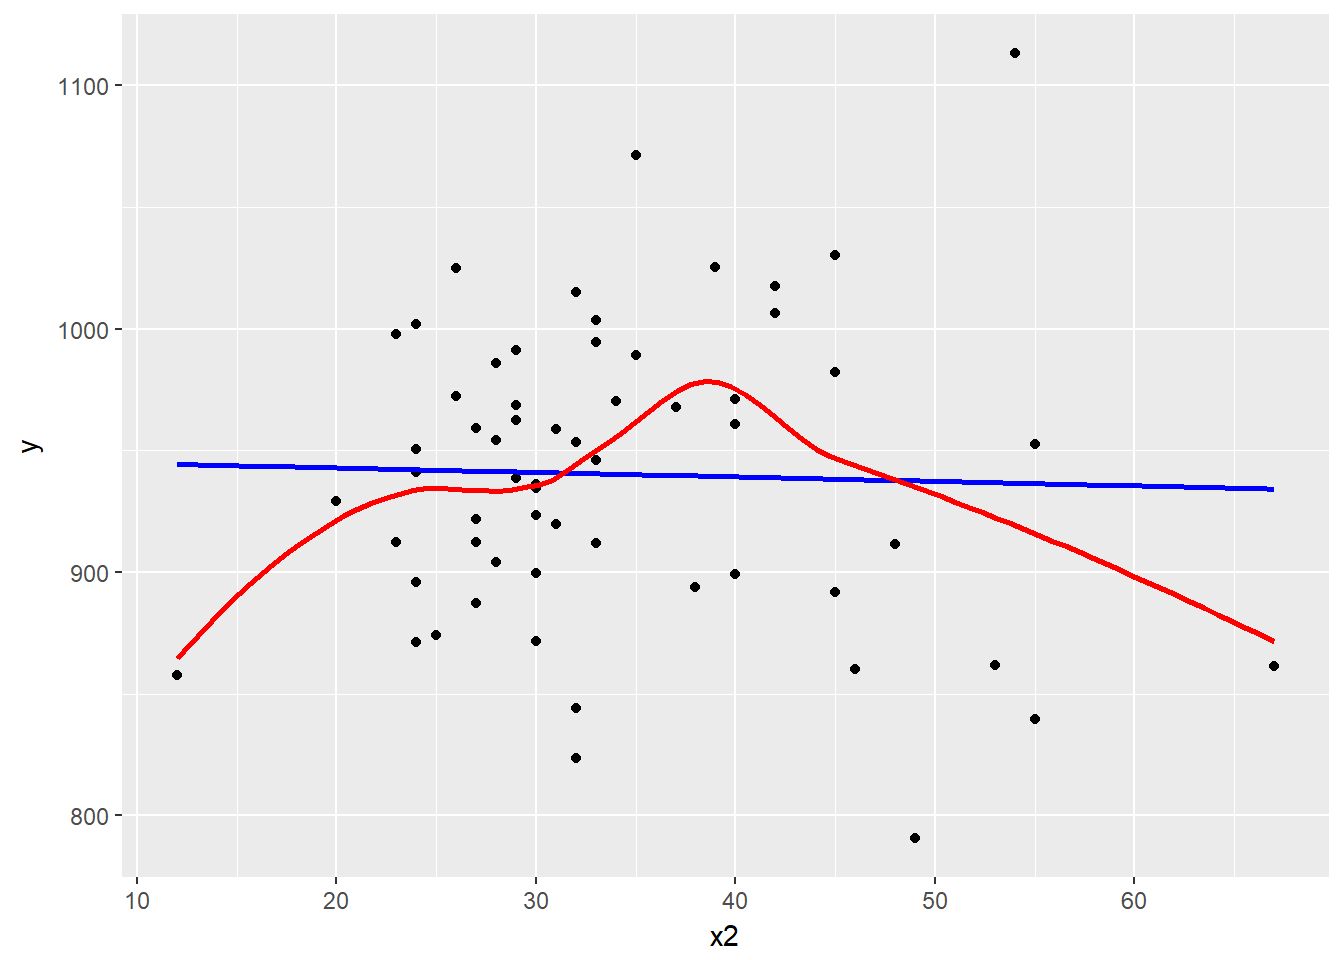
\includegraphics{bookdown-demo_files/figure-latex/c9_lm_and_loess_y_on_x2-1.pdf}

Suppose we plot the residuals that emerge from the linear model shown in
blue, above. Do we see a curve in a plot of residuals against fitted
values?

\begin{Shaded}
\begin{Highlighting}[]
\KeywordTok{plot}\NormalTok{(}\KeywordTok{lm}\NormalTok{(y }\OperatorTok{~}\StringTok{ }\NormalTok{x2, }\DataTypeTok{data =}\NormalTok{ pollution), }\DataTypeTok{which =} \DecValTok{1}\NormalTok{)}
\end{Highlighting}
\end{Shaded}

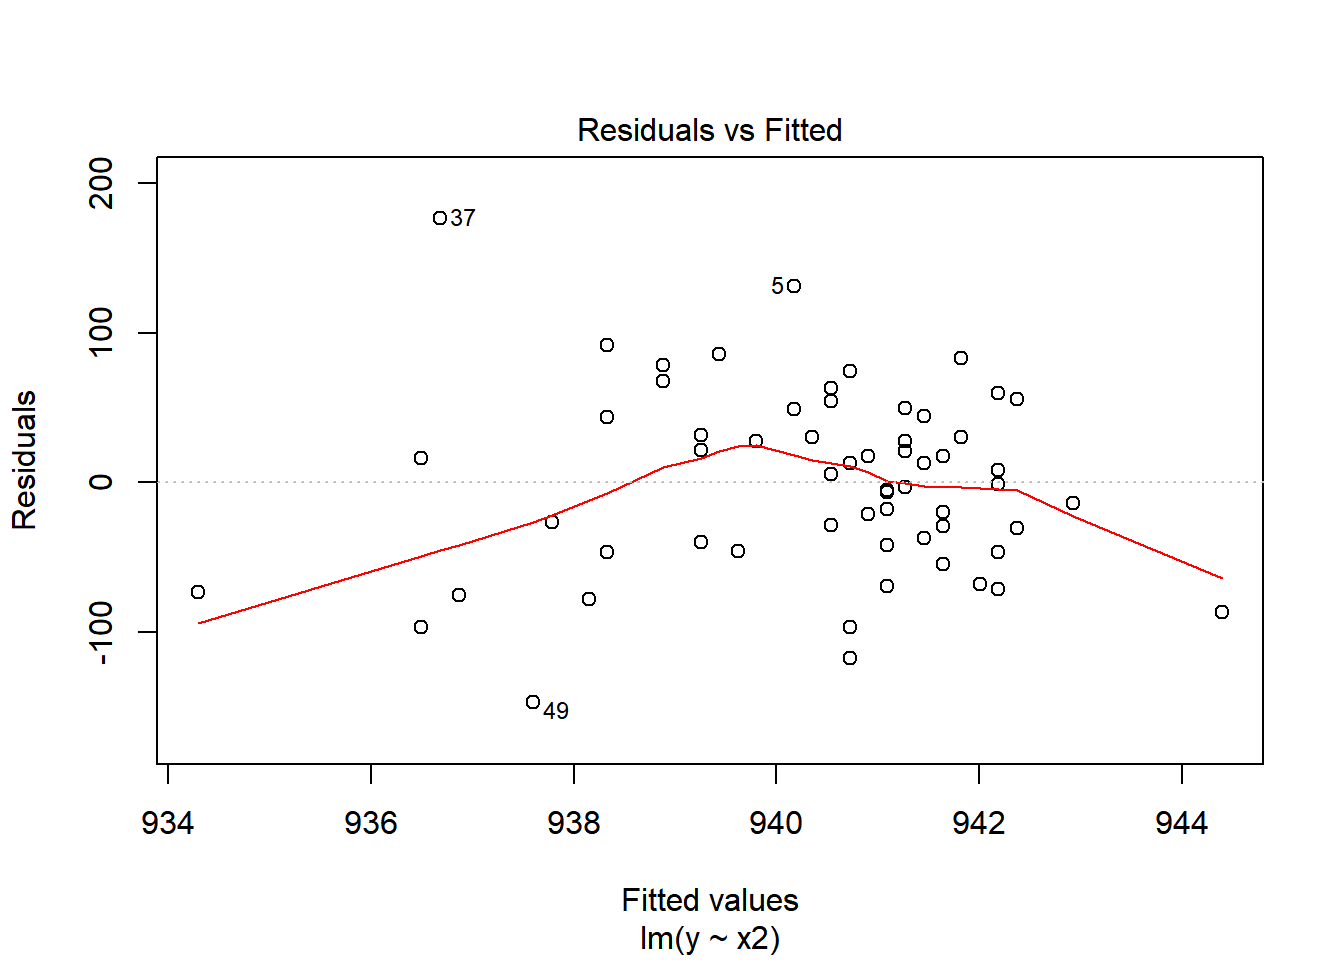
\includegraphics{bookdown-demo_files/figure-latex/fit_c9_m1_and_check_residuals_for_curve-1.pdf}

\section{\texorpdfstring{Quadratic polynomial model to predict
\texttt{y} using
\texttt{x2}}{Quadratic polynomial model to predict y using x2}}\label{quadratic-polynomial-model-to-predict-y-using-x2}

A polynomial in the variable \texttt{x} of degree D is a linear
combination of the powers of \texttt{x} up to D.

For example:

\begin{itemize}
\tightlist
\item
  Linear: \(y = \beta_0 + \beta_1 x\)
\item
  Quadratic: \(y = \beta_0 + \beta_1 x + \beta_2 x^2\)
\item
  Cubic: \(y = \beta_0 + \beta_1 x + \beta_2 x^2 + \beta_3 x^3\)
\item
  Quartic:
  \(y = \beta_0 + \beta_1 x + \beta_2 x^2 + \beta_3 x^3 + \beta_4 x^4\)
\item
  Quintic:
  \(y = \beta_0 + \beta_1 x + \beta_2 x^2 + \beta_3 x^3 + \beta_4 x^4 + \beta_5 x^5\)
\end{itemize}

Fitting such a model creates a **polynomial regression*.

\subsection{The raw quadratic model}\label{the-raw-quadratic-model}

Let's look at a \textbf{quadratic model} which predicts \texttt{y} using
\texttt{x2} and the square of \texttt{x2}, so that our model is of the
form:

\[
y = \beta_0 + \beta_1 x_2 + \beta_2 x_2^2 + error
\]

There are several ways to fit this exact model.

\begin{itemize}
\tightlist
\item
  One approach is to calculate the square of \texttt{x2} within our
  \texttt{pollution} data set, and then feed both \texttt{x2} and
  \texttt{x2squared} to \texttt{lm}.
\item
  Another approach uses the I function within our \texttt{lm} to specify
  the use of both \texttt{x2} and its square.
\item
  Yet another approach uses the \texttt{poly} function within our
  \texttt{lm}, which can be used to specify raw models including
  \texttt{x2} and \texttt{x2squared}.
\end{itemize}

\begin{Shaded}
\begin{Highlighting}[]
\NormalTok{pollution <-}\StringTok{ }\NormalTok{pollution }\OperatorTok
\StringTok{    }\KeywordTok{mutate}\NormalTok{(}\DataTypeTok{x2squared =}\NormalTok{ x2}\OperatorTok{^}\DecValTok{2}\NormalTok{)}

\NormalTok{mod2a <-}\StringTok{ }\KeywordTok{lm}\NormalTok{(y }\OperatorTok{~}\StringTok{ }\NormalTok{x2 }\OperatorTok{+}\StringTok{ }\NormalTok{x2squared, }\DataTypeTok{data =}\NormalTok{ pollution)}
\NormalTok{mod2b <-}\StringTok{ }\KeywordTok{lm}\NormalTok{(y }\OperatorTok{~}\StringTok{ }\NormalTok{x2 }\OperatorTok{+}\StringTok{ }\KeywordTok{I}\NormalTok{(x2}\OperatorTok{^}\DecValTok{2}\NormalTok{), }\DataTypeTok{data =}\NormalTok{ pollution)}
\NormalTok{mod2c <-}\StringTok{ }\KeywordTok{lm}\NormalTok{(y }\OperatorTok{~}\StringTok{ }\KeywordTok{poly}\NormalTok{(x2, }\DataTypeTok{degree =} \DecValTok{2}\NormalTok{, }\DataTypeTok{raw =} \OtherTok{TRUE}\NormalTok{), }\DataTypeTok{data =}\NormalTok{ pollution)}
\end{Highlighting}
\end{Shaded}

Each of these approaches produces the same model, as they are just
different ways of expressing the same idea.

\begin{Shaded}
\begin{Highlighting}[]
\KeywordTok{summary}\NormalTok{(mod2a)}
\end{Highlighting}
\end{Shaded}

\begin{verbatim}

Call:
lm(formula = y ~ x2 + x2squared, data = pollution)

Residuals:
     Min       1Q   Median       3Q      Max 
-148.977  -38.651    6.889   35.312  189.346 

Coefficients:
             Estimate Std. Error t value Pr(>|t|)    
(Intercept) 785.77449   79.54086   9.879 5.87e-14 ***
x2            8.87640    4.27394   2.077   0.0423 *  
x2squared    -0.11704    0.05429  -2.156   0.0353 *  
---
Signif. codes:  0 '***' 0.001 '**' 0.01 '*' 0.05 '.' 0.1 ' ' 1

Residual standard error: 60.83 on 57 degrees of freedom
Multiple R-squared:  0.07623,   Adjusted R-squared:  0.04382 
F-statistic: 2.352 on 2 and 57 DF,  p-value: 0.1044
\end{verbatim}

And if we plot the fitted values for this \texttt{mod2} using whatever
approach you like, we get exactly the same result.

\begin{Shaded}
\begin{Highlighting}[]
\NormalTok{mod2a.aug <-}\StringTok{ }\KeywordTok{augment}\NormalTok{(mod2a, pollution)}

\KeywordTok{ggplot}\NormalTok{(mod2a.aug, }\KeywordTok{aes}\NormalTok{(}\DataTypeTok{x =}\NormalTok{ x2, }\DataTypeTok{y =}\NormalTok{ y)) }\OperatorTok{+}
\StringTok{    }\KeywordTok{geom_point}\NormalTok{() }\OperatorTok{+}
\StringTok{    }\KeywordTok{geom_line}\NormalTok{(}\KeywordTok{aes}\NormalTok{(}\DataTypeTok{x =}\NormalTok{ x2, }\DataTypeTok{y =}\NormalTok{ .fitted), }\DataTypeTok{col =} \StringTok{"red"}\NormalTok{) }\OperatorTok{+}
\StringTok{    }\KeywordTok{labs}\NormalTok{(}\DataTypeTok{title =} \StringTok{"Model 2a: Quadratic fit using x2 and x2^2"}\NormalTok{)}
\end{Highlighting}
\end{Shaded}

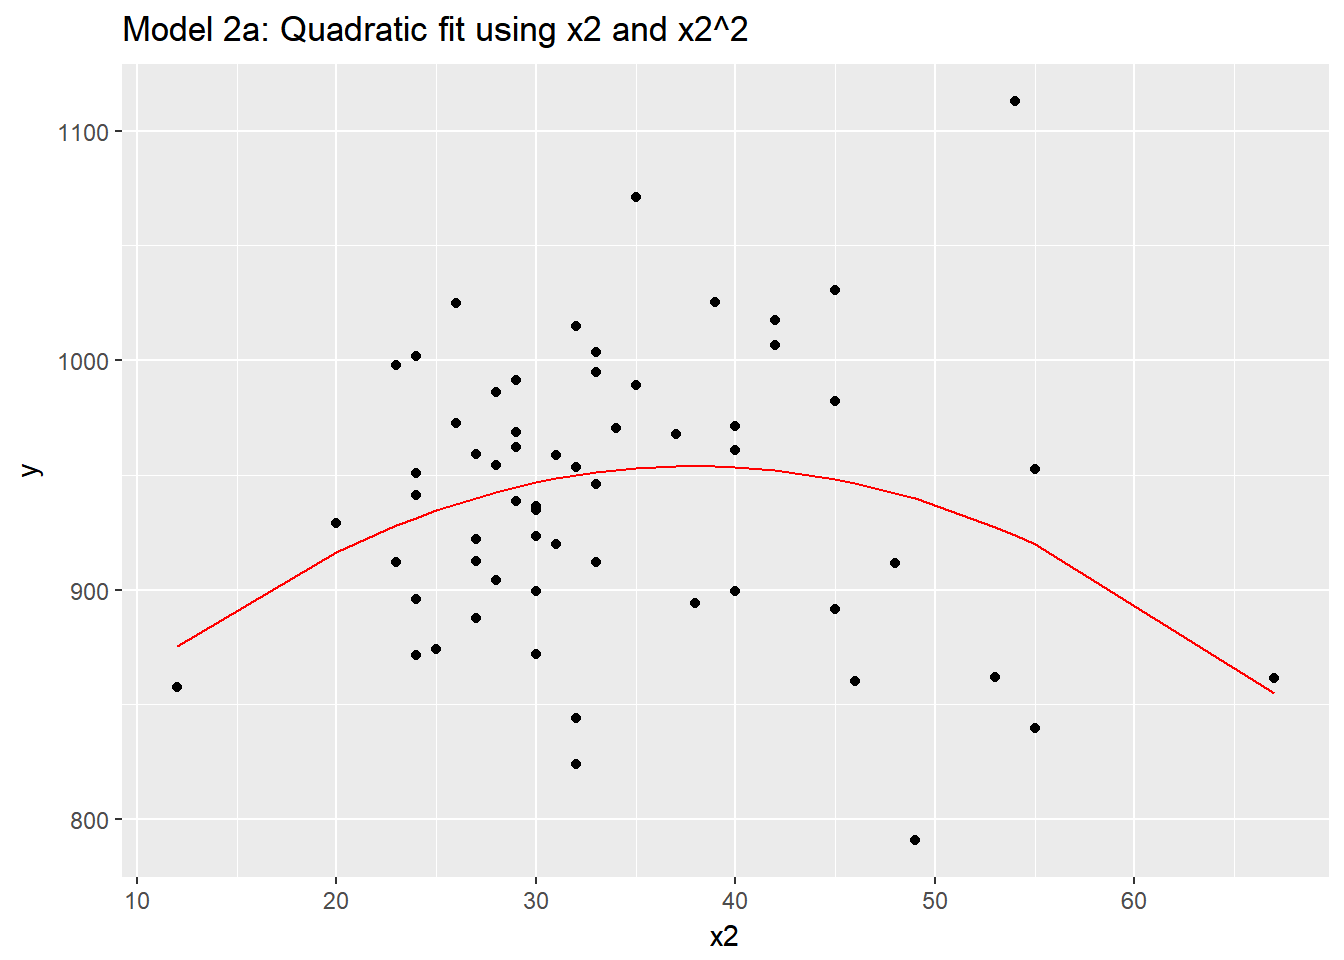
\includegraphics{bookdown-demo_files/figure-latex/unnamed-chunk-94-1.pdf}

\begin{Shaded}
\begin{Highlighting}[]
\NormalTok{mod2b.aug <-}\StringTok{ }\KeywordTok{augment}\NormalTok{(mod2b, pollution)}

\NormalTok{mod2c.aug <-}\StringTok{ }\KeywordTok{augment}\NormalTok{(mod2c, pollution)}

\NormalTok{p1 <-}\StringTok{ }\KeywordTok{ggplot}\NormalTok{(mod2b.aug, }\KeywordTok{aes}\NormalTok{(}\DataTypeTok{x =}\NormalTok{ x2, }\DataTypeTok{y =}\NormalTok{ y)) }\OperatorTok{+}
\StringTok{    }\KeywordTok{geom_point}\NormalTok{() }\OperatorTok{+}
\StringTok{    }\KeywordTok{geom_line}\NormalTok{(}\KeywordTok{aes}\NormalTok{(}\DataTypeTok{x =}\NormalTok{ x2, }\DataTypeTok{y =}\NormalTok{ .fitted), }\DataTypeTok{col =} \StringTok{"red"}\NormalTok{) }\OperatorTok{+}
\StringTok{    }\KeywordTok{labs}\NormalTok{(}\DataTypeTok{title =} \StringTok{"Model 2b: Quadratic fit"}\NormalTok{)}

\NormalTok{p2 <-}\StringTok{ }\KeywordTok{ggplot}\NormalTok{(mod2c.aug, }\KeywordTok{aes}\NormalTok{(}\DataTypeTok{x =}\NormalTok{ x2, }\DataTypeTok{y =}\NormalTok{ y)) }\OperatorTok{+}
\StringTok{    }\KeywordTok{geom_point}\NormalTok{() }\OperatorTok{+}
\StringTok{    }\KeywordTok{geom_line}\NormalTok{(}\KeywordTok{aes}\NormalTok{(}\DataTypeTok{x =}\NormalTok{ x2, }\DataTypeTok{y =}\NormalTok{ .fitted), }\DataTypeTok{col =} \StringTok{"blue"}\NormalTok{) }\OperatorTok{+}
\StringTok{    }\KeywordTok{labs}\NormalTok{(}\DataTypeTok{title =} \StringTok{"Model 2c: Quadratic fit"}\NormalTok{)}

\NormalTok{gridExtra}\OperatorTok{::}\KeywordTok{grid.arrange}\NormalTok{(p1, p2, }\DataTypeTok{nrow =} \DecValTok{1}\NormalTok{)}
\end{Highlighting}
\end{Shaded}

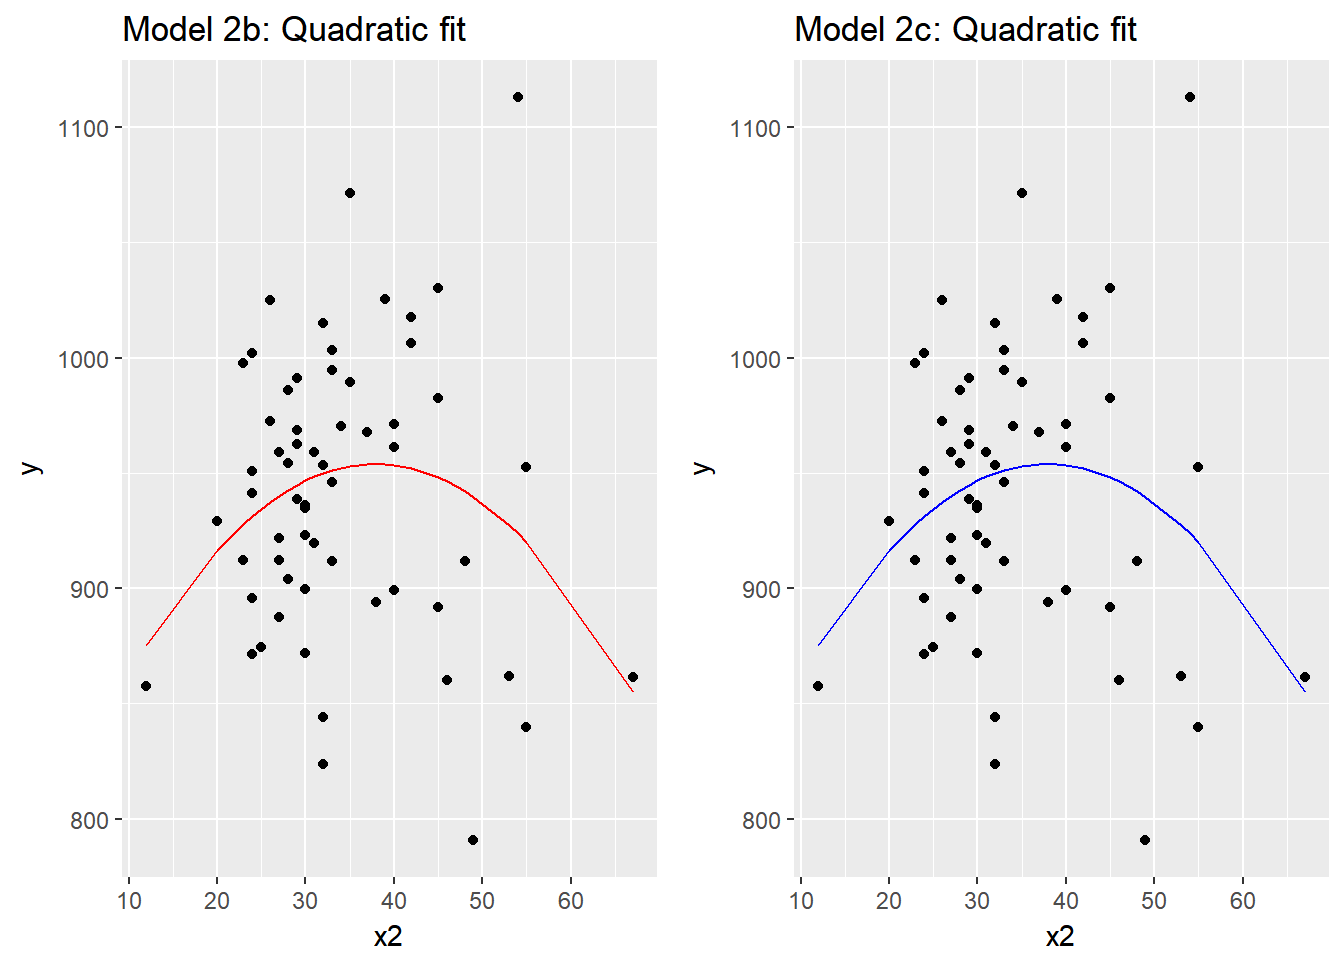
\includegraphics{bookdown-demo_files/figure-latex/unnamed-chunk-95-1.pdf}

\subsection{\texorpdfstring{Raw quadratic fit after centering
\texttt{x2}}{Raw quadratic fit after centering x2}}\label{raw-quadratic-fit-after-centering-x2}

Sometimes, we'll center (and perhaps rescale, too) the x2 variable
before including it in a quadratic fit like this.

\begin{Shaded}
\begin{Highlighting}[]
\NormalTok{pollution <-}\StringTok{ }\NormalTok{pollution }\OperatorTok
\StringTok{    }\KeywordTok{mutate}\NormalTok{(}\DataTypeTok{x2_c =}\NormalTok{ x2 }\OperatorTok{-}\StringTok{ }\KeywordTok{mean}\NormalTok{(x2))}

\NormalTok{mod2d <-}\StringTok{ }\KeywordTok{lm}\NormalTok{(y }\OperatorTok{~}\StringTok{ }\NormalTok{x2_c }\OperatorTok{+}\StringTok{ }\KeywordTok{I}\NormalTok{(x2_c}\OperatorTok{^}\DecValTok{2}\NormalTok{), }\DataTypeTok{data =}\NormalTok{ pollution)}

\KeywordTok{summary}\NormalTok{(mod2d)}
\end{Highlighting}
\end{Shaded}

\begin{verbatim}

Call:
lm(formula = y ~ x2_c + I(x2_c^2), data = pollution)

Residuals:
     Min       1Q   Median       3Q      Max 
-148.977  -38.651    6.889   35.312  189.346 

Coefficients:
             Estimate Std. Error t value Pr(>|t|)    
(Intercept) 952.25941    9.59896  99.204   <2e-16 ***
x2_c          0.92163    0.93237   0.988   0.3271    
I(x2_c^2)    -0.11704    0.05429  -2.156   0.0353 *  
---
Signif. codes:  0 '***' 0.001 '**' 0.01 '*' 0.05 '.' 0.1 ' ' 1

Residual standard error: 60.83 on 57 degrees of freedom
Multiple R-squared:  0.07623,   Adjusted R-squared:  0.04382 
F-statistic: 2.352 on 2 and 57 DF,  p-value: 0.1044
\end{verbatim}

Note that this model looks very different, with the exception of the
second order quadratic term. But, it produces the same fitted values as
the models we fit previously.

\begin{Shaded}
\begin{Highlighting}[]
\NormalTok{mod2d.aug <-}\StringTok{ }\KeywordTok{augment}\NormalTok{(mod2d, pollution)}

\KeywordTok{ggplot}\NormalTok{(mod2d.aug, }\KeywordTok{aes}\NormalTok{(}\DataTypeTok{x =}\NormalTok{ x2, }\DataTypeTok{y =}\NormalTok{ y)) }\OperatorTok{+}
\StringTok{    }\KeywordTok{geom_point}\NormalTok{() }\OperatorTok{+}
\StringTok{    }\KeywordTok{geom_line}\NormalTok{(}\KeywordTok{aes}\NormalTok{(}\DataTypeTok{x =}\NormalTok{ x2, }\DataTypeTok{y =}\NormalTok{ .fitted), }\DataTypeTok{col =} \StringTok{"red"}\NormalTok{) }\OperatorTok{+}
\StringTok{    }\KeywordTok{labs}\NormalTok{(}\DataTypeTok{title =} \StringTok{"Model 2d: Quadratic fit using centered x2 and x2^2"}\NormalTok{)}
\end{Highlighting}
\end{Shaded}

\includegraphics{bookdown-demo_files/figure-latex/unnamed-chunk-97-1.pdf}

Or, if you don't believe me yet, look at the four sets of fitted values
another way.

\begin{Shaded}
\begin{Highlighting}[]
\NormalTok{mod2a.aug }\OperatorTok\StringTok{ }\KeywordTok{skim}\NormalTok{(.fitted)}
\end{Highlighting}
\end{Shaded}

\begin{verbatim}
Skim summary statistics
 n obs: 60 
 n variables: 24 

Variable type: numeric 
 variable missing complete  n   mean    sd    p0    p25 median    p75
  .fitted       0       60 60 940.36 17.18 855.1 936.72  945.6 950.29
   p100
 954.07
\end{verbatim}

\begin{Shaded}
\begin{Highlighting}[]
\NormalTok{mod2b.aug }\OperatorTok\StringTok{ }\KeywordTok{skim}\NormalTok{(.fitted)}
\end{Highlighting}
\end{Shaded}

\begin{verbatim}
Skim summary statistics
 n obs: 60 
 n variables: 24 

Variable type: numeric 
 variable missing complete  n   mean    sd    p0    p25 median    p75
  .fitted       0       60 60 940.36 17.18 855.1 936.72  945.6 950.29
   p100
 954.07
\end{verbatim}

\begin{Shaded}
\begin{Highlighting}[]
\NormalTok{mod2c.aug }\OperatorTok\StringTok{ }\KeywordTok{skim}\NormalTok{(.fitted)}
\end{Highlighting}
\end{Shaded}

\begin{verbatim}
Skim summary statistics
 n obs: 60 
 n variables: 24 

Variable type: numeric 
 variable missing complete  n   mean    sd    p0    p25 median    p75
  .fitted       0       60 60 940.36 17.18 855.1 936.72  945.6 950.29
   p100
 954.07
\end{verbatim}

\begin{Shaded}
\begin{Highlighting}[]
\NormalTok{mod2d.aug }\OperatorTok\StringTok{ }\KeywordTok{skim}\NormalTok{(.fitted)}
\end{Highlighting}
\end{Shaded}

\begin{verbatim}
Skim summary statistics
 n obs: 60 
 n variables: 25 

Variable type: numeric 
 variable missing complete  n   mean    sd    p0    p25 median    p75
  .fitted       0       60 60 940.36 17.18 855.1 936.72  945.6 950.29
   p100
 954.07
\end{verbatim}

\section{Orthogonal Polynomials}\label{orthogonal-polynomials}

Now, let's fit an orthogonal polynomial of degree 2 to predict
\texttt{y} using \texttt{x2}.

\begin{Shaded}
\begin{Highlighting}[]
\NormalTok{mod2_orth <-}\StringTok{ }\KeywordTok{lm}\NormalTok{(y }\OperatorTok{~}\StringTok{ }\KeywordTok{poly}\NormalTok{(x2, }\DecValTok{2}\NormalTok{), }\DataTypeTok{data =}\NormalTok{ pollution)}

\KeywordTok{summary}\NormalTok{(mod2_orth)}
\end{Highlighting}
\end{Shaded}

\begin{verbatim}

Call:
lm(formula = y ~ poly(x2, 2), data = pollution)

Residuals:
     Min       1Q   Median       3Q      Max 
-148.977  -38.651    6.889   35.312  189.346 

Coefficients:
             Estimate Std. Error t value Pr(>|t|)    
(Intercept)   940.358      7.853 119.746   <2e-16 ***
poly(x2, 2)1  -14.345     60.829  -0.236   0.8144    
poly(x2, 2)2 -131.142     60.829  -2.156   0.0353 *  
---
Signif. codes:  0 '***' 0.001 '**' 0.01 '*' 0.05 '.' 0.1 ' ' 1

Residual standard error: 60.83 on 57 degrees of freedom
Multiple R-squared:  0.07623,   Adjusted R-squared:  0.04382 
F-statistic: 2.352 on 2 and 57 DF,  p-value: 0.1044
\end{verbatim}

Now this looks very different in the equation, but, again, we can see
that this produces exactly the same fitted values as our previous
models, and the same model fit summaries. Is it, in fact, the same
model? Here, we'll plot the fitted Model 2a in a red line, and this new
Model 2 with Orthogonal Polynomials as blue points.

\begin{Shaded}
\begin{Highlighting}[]
\NormalTok{mod2orth.aug <-}\StringTok{ }\KeywordTok{augment}\NormalTok{(mod2_orth, pollution)}

\KeywordTok{ggplot}\NormalTok{(mod2orth.aug, }\KeywordTok{aes}\NormalTok{(}\DataTypeTok{x =}\NormalTok{ x2, }\DataTypeTok{y =}\NormalTok{ y)) }\OperatorTok{+}
\StringTok{    }\KeywordTok{geom_point}\NormalTok{() }\OperatorTok{+}
\StringTok{    }\KeywordTok{geom_point}\NormalTok{(}\KeywordTok{aes}\NormalTok{(}\DataTypeTok{x =}\NormalTok{ x2, }\DataTypeTok{y =}\NormalTok{ .fitted), }
               \DataTypeTok{col =} \StringTok{"blue"}\NormalTok{, }\DataTypeTok{size =} \DecValTok{2}\NormalTok{) }\OperatorTok{+}
\StringTok{    }\KeywordTok{geom_line}\NormalTok{(}\DataTypeTok{data =}\NormalTok{ mod2a.aug, }\KeywordTok{aes}\NormalTok{(}\DataTypeTok{x =}\NormalTok{ x2, }\DataTypeTok{y =}\NormalTok{ .fitted),}
              \DataTypeTok{col =} \StringTok{"red"}\NormalTok{) }\OperatorTok{+}
\StringTok{    }\KeywordTok{labs}\NormalTok{(}\DataTypeTok{title =} \StringTok{"Model 2 with Orthogonal Polynomial, degree 2"}\NormalTok{)}
\end{Highlighting}
\end{Shaded}

\includegraphics{bookdown-demo_files/figure-latex/unnamed-chunk-100-1.pdf}

Yes, it is again the same model in terms of the predictions it makes for
\texttt{y}.

By default, with \texttt{raw\ =\ FALSE}, the \texttt{poly()} function
within a linear model computes what is called an \textbf{orthogonal
polynomial}. An orthogonal polynomial sets up a model design matrix
using the coding we've seen previously: \texttt{x2} and \texttt{x2}\^{}2
in our case, and then scales those columns so that each column is
\textbf{orthogonal} to the previous ones. This eliminates the
collinearity (correlation between predictors) and lets our t tests tell
us whether the addition of any particular polynomial term improves the
fit of the model over the lower orders.

Would the addition of a cubic term help us much in predicting \texttt{y}
from \texttt{x2}?

\begin{Shaded}
\begin{Highlighting}[]
\NormalTok{mod3 <-}\StringTok{ }\KeywordTok{lm}\NormalTok{(y }\OperatorTok{~}\StringTok{ }\KeywordTok{poly}\NormalTok{(x2, }\DecValTok{3}\NormalTok{), }\DataTypeTok{data =}\NormalTok{ pollution)}
\KeywordTok{summary}\NormalTok{(mod3)}
\end{Highlighting}
\end{Shaded}

\begin{verbatim}

Call:
lm(formula = y ~ poly(x2, 3), data = pollution)

Residuals:
     Min       1Q   Median       3Q      Max 
-146.262  -39.679    5.569   35.984  191.536 

Coefficients:
             Estimate Std. Error t value Pr(>|t|)    
(Intercept)   940.358      7.917 118.772   <2e-16 ***
poly(x2, 3)1  -14.345     61.328  -0.234   0.8159    
poly(x2, 3)2 -131.142     61.328  -2.138   0.0369 *  
poly(x2, 3)3   16.918     61.328   0.276   0.7837    
---
Signif. codes:  0 '***' 0.001 '**' 0.01 '*' 0.05 '.' 0.1 ' ' 1

Residual standard error: 61.33 on 56 degrees of freedom
Multiple R-squared:  0.07748,   Adjusted R-squared:  0.02806 
F-statistic: 1.568 on 3 and 56 DF,  p-value: 0.2073
\end{verbatim}

It doesn't appear that the cubic term adds much here, if anything. The
\emph{p} value is not significant for the third degree polynomial, the
summaries of fit quality aren't much improved, and as we can see from
the plot below, the predictions don't actually change all that much.

\begin{Shaded}
\begin{Highlighting}[]
\NormalTok{mod3.aug <-}\StringTok{ }\KeywordTok{augment}\NormalTok{(mod3, pollution)}

\KeywordTok{ggplot}\NormalTok{(mod3.aug, }\KeywordTok{aes}\NormalTok{(}\DataTypeTok{x =}\NormalTok{ x2, }\DataTypeTok{y =}\NormalTok{ y)) }\OperatorTok{+}
\StringTok{    }\KeywordTok{geom_point}\NormalTok{() }\OperatorTok{+}
\StringTok{    }\KeywordTok{geom_line}\NormalTok{(}\KeywordTok{aes}\NormalTok{(}\DataTypeTok{x =}\NormalTok{ x2, }\DataTypeTok{y =}\NormalTok{ .fitted), }
              \DataTypeTok{col =} \StringTok{"blue"}\NormalTok{) }\OperatorTok{+}
\StringTok{    }\KeywordTok{geom_line}\NormalTok{(}\DataTypeTok{data =}\NormalTok{ mod2orth.aug, }\KeywordTok{aes}\NormalTok{(}\DataTypeTok{x =}\NormalTok{ x2, }\DataTypeTok{y =}\NormalTok{ .fitted),}
              \DataTypeTok{col =} \StringTok{"red"}\NormalTok{) }\OperatorTok{+}
\StringTok{    }\KeywordTok{labs}\NormalTok{(}\DataTypeTok{title =} \StringTok{"Quadratic (red) vs. Cubic (blue) Polynomial Fits"}\NormalTok{)}
\end{Highlighting}
\end{Shaded}

\includegraphics{bookdown-demo_files/figure-latex/unnamed-chunk-102-1.pdf}

\section{\texorpdfstring{Fit a cubic polynomial to predict \texttt{y}
from
\texttt{x3}}{Fit a cubic polynomial to predict y from x3}}\label{fit-a-cubic-polynomial-to-predict-y-from-x3}

What if we consider another predictor instead? Let's look at
\texttt{x3}, the Mean July temperature in degrees Fahrenheit. Here is
the \texttt{loess} smooth.

\begin{Shaded}
\begin{Highlighting}[]
\KeywordTok{ggplot}\NormalTok{(pollution, }\KeywordTok{aes}\NormalTok{(}\DataTypeTok{x =}\NormalTok{ x3, }\DataTypeTok{y =}\NormalTok{ y)) }\OperatorTok{+}
\StringTok{    }\KeywordTok{geom_point}\NormalTok{() }\OperatorTok{+}
\StringTok{    }\KeywordTok{geom_smooth}\NormalTok{(}\DataTypeTok{method =} \StringTok{"loess"}\NormalTok{)}
\end{Highlighting}
\end{Shaded}

\includegraphics{bookdown-demo_files/figure-latex/unnamed-chunk-103-1.pdf}

That looks pretty curvy - perhaps we need a more complex polynomial.
We'll consider a linear model (\texttt{mod4\_L}), a quadratic fit
(\texttt{mod4\_Q}) and a polynomial of degree 3: a \textbf{cubic} fit
(\texttt{mod\_4C})

\begin{Shaded}
\begin{Highlighting}[]
\NormalTok{mod4_L <-}\StringTok{ }\KeywordTok{lm}\NormalTok{(y }\OperatorTok{~}\StringTok{ }\NormalTok{x3, }\DataTypeTok{data =}\NormalTok{ pollution)}
\KeywordTok{summary}\NormalTok{(mod4_L)}
\end{Highlighting}
\end{Shaded}

\begin{verbatim}

Call:
lm(formula = y ~ x3, data = pollution)

Residuals:
     Min       1Q   Median       3Q      Max 
-139.813  -34.341    4.271   38.197  149.587 

Coefficients:
            Estimate Std. Error t value Pr(>|t|)    
(Intercept)  670.529    123.140   5.445  1.1e-06 ***
x3             3.618      1.648   2.196   0.0321 *  
---
Signif. codes:  0 '***' 0.001 '**' 0.01 '*' 0.05 '.' 0.1 ' ' 1

Residual standard error: 60.29 on 58 degrees of freedom
Multiple R-squared:  0.07674,   Adjusted R-squared:  0.06082 
F-statistic: 4.821 on 1 and 58 DF,  p-value: 0.03213
\end{verbatim}

\begin{Shaded}
\begin{Highlighting}[]
\NormalTok{mod4_Q <-}\StringTok{ }\KeywordTok{lm}\NormalTok{(y }\OperatorTok{~}\StringTok{ }\KeywordTok{poly}\NormalTok{(x3, }\DecValTok{2}\NormalTok{), }\DataTypeTok{data =}\NormalTok{ pollution)}
\KeywordTok{summary}\NormalTok{(mod4_Q)}
\end{Highlighting}
\end{Shaded}

\begin{verbatim}

Call:
lm(formula = y ~ poly(x3, 2), data = pollution)

Residuals:
     Min       1Q   Median       3Q      Max 
-132.004  -42.184    4.069   47.126  157.396 

Coefficients:
             Estimate Std. Error t value Pr(>|t|)    
(Intercept)   940.358      7.553 124.503   <2e-16 ***
poly(x3, 2)1  132.364     58.504   2.262   0.0275 *  
poly(x3, 2)2 -125.270     58.504  -2.141   0.0365 *  
---
Signif. codes:  0 '***' 0.001 '**' 0.01 '*' 0.05 '.' 0.1 ' ' 1

Residual standard error: 58.5 on 57 degrees of freedom
Multiple R-squared:  0.1455,    Adjusted R-squared:  0.1155 
F-statistic: 4.852 on 2 and 57 DF,  p-value: 0.01133
\end{verbatim}

\begin{Shaded}
\begin{Highlighting}[]
\NormalTok{mod4_C <-}\StringTok{ }\KeywordTok{lm}\NormalTok{(y }\OperatorTok{~}\StringTok{ }\KeywordTok{poly}\NormalTok{(x3, }\DecValTok{3}\NormalTok{), }\DataTypeTok{data =}\NormalTok{ pollution)}
\KeywordTok{summary}\NormalTok{(mod4_C)}
\end{Highlighting}
\end{Shaded}

\begin{verbatim}

Call:
lm(formula = y ~ poly(x3, 3), data = pollution)

Residuals:
     Min       1Q   Median       3Q      Max 
-148.004  -29.998    1.441   34.579  141.396 

Coefficients:
             Estimate Std. Error t value Pr(>|t|)    
(Intercept)   940.358      7.065 133.095  < 2e-16 ***
poly(x3, 3)1  132.364     54.728   2.419  0.01886 *  
poly(x3, 3)2 -125.270     54.728  -2.289  0.02588 *  
poly(x3, 3)3 -165.439     54.728  -3.023  0.00377 ** 
---
Signif. codes:  0 '***' 0.001 '**' 0.01 '*' 0.05 '.' 0.1 ' ' 1

Residual standard error: 54.73 on 56 degrees of freedom
Multiple R-squared:  0.2654,    Adjusted R-squared:  0.226 
F-statistic: 6.742 on 3 and 56 DF,  p-value: 0.0005799
\end{verbatim}

It looks like the cubic polynomial term is of some real importance here.
Do the linear, quadratic and cubic model fitted values look different?

\begin{Shaded}
\begin{Highlighting}[]
\NormalTok{mod4_L.aug <-}\StringTok{ }\KeywordTok{augment}\NormalTok{(mod4_L, pollution)}

\NormalTok{mod4_Q.aug <-}\StringTok{ }\KeywordTok{augment}\NormalTok{(mod4_Q, pollution)}

\NormalTok{mod4_C.aug <-}\StringTok{ }\KeywordTok{augment}\NormalTok{(mod4_C, pollution)}

\KeywordTok{ggplot}\NormalTok{(pollution, }\KeywordTok{aes}\NormalTok{(}\DataTypeTok{x =}\NormalTok{ x3, }\DataTypeTok{y =}\NormalTok{ y)) }\OperatorTok{+}
\StringTok{    }\KeywordTok{geom_point}\NormalTok{() }\OperatorTok{+}
\StringTok{    }\KeywordTok{geom_line}\NormalTok{(}\DataTypeTok{data =}\NormalTok{ mod4_L.aug, }\KeywordTok{aes}\NormalTok{(}\DataTypeTok{x =}\NormalTok{ x3, }\DataTypeTok{y =}\NormalTok{ .fitted), }
              \DataTypeTok{col =} \StringTok{"blue"}\NormalTok{, }\DataTypeTok{size =} \FloatTok{1.25}\NormalTok{) }\OperatorTok{+}
\StringTok{    }\KeywordTok{geom_line}\NormalTok{(}\DataTypeTok{data =}\NormalTok{ mod4_Q.aug, }\KeywordTok{aes}\NormalTok{(}\DataTypeTok{x =}\NormalTok{ x3, }\DataTypeTok{y =}\NormalTok{ .fitted),}
              \DataTypeTok{col =} \StringTok{"black"}\NormalTok{, }\DataTypeTok{size =} \FloatTok{1.25}\NormalTok{) }\OperatorTok{+}
\StringTok{    }\KeywordTok{geom_line}\NormalTok{(}\DataTypeTok{data =}\NormalTok{ mod4_C.aug, }\KeywordTok{aes}\NormalTok{(}\DataTypeTok{x =}\NormalTok{ x3, }\DataTypeTok{y =}\NormalTok{ .fitted),}
              \DataTypeTok{col =} \StringTok{"red"}\NormalTok{, }\DataTypeTok{size =} \FloatTok{1.25}\NormalTok{) }\OperatorTok{+}
\StringTok{    }\KeywordTok{geom_text}\NormalTok{(}\DataTypeTok{x =} \DecValTok{66}\NormalTok{, }\DataTypeTok{y =} \DecValTok{930}\NormalTok{, }\DataTypeTok{label =} \StringTok{"Linear Fit"}\NormalTok{, }\DataTypeTok{col =} \StringTok{"blue"}\NormalTok{) }\OperatorTok{+}
\StringTok{    }\KeywordTok{geom_text}\NormalTok{(}\DataTypeTok{x =} \DecValTok{64}\NormalTok{, }\DataTypeTok{y =} \DecValTok{820}\NormalTok{, }\DataTypeTok{label =} \StringTok{"Quadratic Fit"}\NormalTok{, }\DataTypeTok{col =} \StringTok{"black"}\NormalTok{) }\OperatorTok{+}
\StringTok{    }\KeywordTok{geom_text}\NormalTok{(}\DataTypeTok{x =} \DecValTok{83}\NormalTok{, }\DataTypeTok{y =} \DecValTok{900}\NormalTok{, }\DataTypeTok{label =} \StringTok{"Cubic Fit"}\NormalTok{, }\DataTypeTok{col =} \StringTok{"red"}\NormalTok{) }\OperatorTok{+}
\StringTok{    }\KeywordTok{labs}\NormalTok{(}\DataTypeTok{title =} \StringTok{"Linear, Quadratic and Cubic Fits predicting y with x3"}\NormalTok{) }\OperatorTok{+}
\StringTok{    }\KeywordTok{theme_bw}\NormalTok{()}
\end{Highlighting}
\end{Shaded}

\includegraphics{bookdown-demo_files/figure-latex/unnamed-chunk-105-1.pdf}

\section{Fitting a restricted cubic spline in a linear
regression}\label{fitting-a-restricted-cubic-spline-in-a-linear-regression}

\begin{itemize}
\tightlist
\item
  A \textbf{linear spline} is a continuous function formed by connecting
  points (called \textbf{knots} of the spline) by line segments.
\item
  A \textbf{restricted cubic spline} is a way to build highly
  complicated curves into a regression equation in a fairly easily
  structured way.
\item
  A restricted cubic spline is a series of polynomial functions joined
  together at the knots.

  \begin{itemize}
  \tightlist
  \item
    Such a spline gives us a way to flexibly account for non-linearity
    without over-fitting the model.
  \item
    Restricted cubic splines can fit many different types of
    non-linearities.
  \item
    Specifying the number of knots is all you need to do in R to get a
    reasonable result from a restricted cubic spline.
  \end{itemize}
\end{itemize}

The most common choices are 3, 4, or 5 knots. Each additional knot adds
to the non-linearity, and spends an additional degree of freedom:

\begin{itemize}
\tightlist
\item
  3 Knots, 2 degrees of freedom, allows the curve to ``bend'' once.
\item
  4 Knots, 3 degrees of freedom, lets the curve ``bend'' twice.
\item
  5 Knots, 4 degrees of freedom, lets the curve ``bend'' three times.
\end{itemize}

For most applications, three to five knots strike a nice balance between
complicating the model needlessly and fitting data pleasingly. Let's
consider a restricted cubic spline model for our \texttt{y} based on
\texttt{x3} again, but now with:

\begin{itemize}
\tightlist
\item
  in \texttt{mod5a}, 3 knots,
\item
  in \texttt{mod5b}, 4 knots, and
\item
  in \texttt{mod5c}, 5 knots
\end{itemize}

\begin{Shaded}
\begin{Highlighting}[]
\NormalTok{mod5a_rcs <-}\StringTok{ }\KeywordTok{lm}\NormalTok{(y }\OperatorTok{~}\StringTok{ }\KeywordTok{rcs}\NormalTok{(x3, }\DecValTok{3}\NormalTok{), }\DataTypeTok{data =}\NormalTok{ pollution)}
\NormalTok{mod5b_rcs <-}\StringTok{ }\KeywordTok{lm}\NormalTok{(y }\OperatorTok{~}\StringTok{ }\KeywordTok{rcs}\NormalTok{(x3, }\DecValTok{4}\NormalTok{), }\DataTypeTok{data =}\NormalTok{ pollution)}
\NormalTok{mod5c_rcs <-}\StringTok{ }\KeywordTok{lm}\NormalTok{(y }\OperatorTok{~}\StringTok{ }\KeywordTok{rcs}\NormalTok{(x3, }\DecValTok{5}\NormalTok{), }\DataTypeTok{data =}\NormalTok{ pollution)}
\end{Highlighting}
\end{Shaded}

Here, for instance, is the summary of the 5-knot model:

\begin{Shaded}
\begin{Highlighting}[]
\KeywordTok{summary}\NormalTok{(mod5c_rcs)}
\end{Highlighting}
\end{Shaded}

\begin{verbatim}

Call:
lm(formula = y ~ rcs(x3, 5), data = pollution)

Residuals:
     Min       1Q   Median       3Q      Max 
-141.522  -32.009    1.674   31.971  147.878 

Coefficients:
                Estimate Std. Error t value Pr(>|t|)
(Intercept)      468.113    396.319   1.181    0.243
rcs(x3, 5)x3       6.447      5.749   1.121    0.267
rcs(x3, 5)x3'    -25.633     46.810  -0.548    0.586
rcs(x3, 5)x3''   323.137    293.065   1.103    0.275
rcs(x3, 5)x3''' -612.578    396.270  -1.546    0.128

Residual standard error: 54.35 on 55 degrees of freedom
Multiple R-squared:  0.2883,    Adjusted R-squared:  0.2366 
F-statistic: 5.571 on 4 and 55 DF,  p-value: 0.0007734
\end{verbatim}

We'll begin by storing the fitted values from these three models and
other summaries, for plotting.

\begin{Shaded}
\begin{Highlighting}[]
\NormalTok{mod5a.aug <-}\StringTok{ }\KeywordTok{augment}\NormalTok{(mod5a_rcs, pollution)}

\NormalTok{mod5b.aug <-}\StringTok{ }\KeywordTok{augment}\NormalTok{(mod5b_rcs, pollution)}

\NormalTok{mod5c.aug <-}\StringTok{ }\KeywordTok{augment}\NormalTok{(mod5c_rcs, pollution)}
\end{Highlighting}
\end{Shaded}

\begin{Shaded}
\begin{Highlighting}[]
\NormalTok{p2 <-}\StringTok{ }\KeywordTok{ggplot}\NormalTok{(pollution, }\KeywordTok{aes}\NormalTok{(}\DataTypeTok{x =}\NormalTok{ x3, }\DataTypeTok{y =}\NormalTok{ y)) }\OperatorTok{+}
\StringTok{    }\KeywordTok{geom_point}\NormalTok{() }\OperatorTok{+}
\StringTok{    }\KeywordTok{geom_smooth}\NormalTok{(}\DataTypeTok{method =} \StringTok{"loess"}\NormalTok{, }\DataTypeTok{col =} \StringTok{"purple"}\NormalTok{, }\DataTypeTok{se =}\NormalTok{ F) }\OperatorTok{+}
\StringTok{    }\KeywordTok{labs}\NormalTok{(}\DataTypeTok{title =} \StringTok{"Loess Smooth"}\NormalTok{) }\OperatorTok{+}
\StringTok{    }\KeywordTok{theme_bw}\NormalTok{()}

\NormalTok{p3 <-}\StringTok{ }\KeywordTok{ggplot}\NormalTok{(mod5a.aug, }\KeywordTok{aes}\NormalTok{(}\DataTypeTok{x =}\NormalTok{ x3, }\DataTypeTok{y =}\NormalTok{ y)) }\OperatorTok{+}
\StringTok{    }\KeywordTok{geom_point}\NormalTok{() }\OperatorTok{+}
\StringTok{    }\KeywordTok{geom_line}\NormalTok{(}\KeywordTok{aes}\NormalTok{(}\DataTypeTok{x =}\NormalTok{ x3, }\DataTypeTok{y =}\NormalTok{ .fitted), }
              \DataTypeTok{col =} \StringTok{"blue"}\NormalTok{, }\DataTypeTok{size =} \FloatTok{1.25}\NormalTok{) }\OperatorTok{+}
\StringTok{    }\KeywordTok{labs}\NormalTok{(}\DataTypeTok{title =} \StringTok{"RCS, 3 knots"}\NormalTok{) }\OperatorTok{+}
\StringTok{    }\KeywordTok{theme_bw}\NormalTok{()}

\NormalTok{p4 <-}\StringTok{ }\KeywordTok{ggplot}\NormalTok{(mod5b.aug, }\KeywordTok{aes}\NormalTok{(}\DataTypeTok{x =}\NormalTok{ x3, }\DataTypeTok{y =}\NormalTok{ y)) }\OperatorTok{+}
\StringTok{    }\KeywordTok{geom_point}\NormalTok{() }\OperatorTok{+}
\StringTok{    }\KeywordTok{geom_line}\NormalTok{(}\KeywordTok{aes}\NormalTok{(}\DataTypeTok{x =}\NormalTok{ x3, }\DataTypeTok{y =}\NormalTok{ .fitted), }
              \DataTypeTok{col =} \StringTok{"black"}\NormalTok{, }\DataTypeTok{size =} \FloatTok{1.25}\NormalTok{) }\OperatorTok{+}
\StringTok{    }\KeywordTok{labs}\NormalTok{(}\DataTypeTok{title =} \StringTok{"RCS, 4 knots"}\NormalTok{) }\OperatorTok{+}
\StringTok{    }\KeywordTok{theme_bw}\NormalTok{()}

\NormalTok{p5 <-}\StringTok{ }\KeywordTok{ggplot}\NormalTok{(mod5c.aug, }\KeywordTok{aes}\NormalTok{(}\DataTypeTok{x =}\NormalTok{ x3, }\DataTypeTok{y =}\NormalTok{ y)) }\OperatorTok{+}
\StringTok{    }\KeywordTok{geom_point}\NormalTok{() }\OperatorTok{+}
\StringTok{    }\KeywordTok{geom_line}\NormalTok{(}\KeywordTok{aes}\NormalTok{(}\DataTypeTok{x =}\NormalTok{ x3, }\DataTypeTok{y =}\NormalTok{ .fitted), }
              \DataTypeTok{col =} \StringTok{"red"}\NormalTok{, }\DataTypeTok{size =} \FloatTok{1.25}\NormalTok{) }\OperatorTok{+}
\StringTok{    }\KeywordTok{labs}\NormalTok{(}\DataTypeTok{title =} \StringTok{"RCS, 5 knots"}\NormalTok{) }\OperatorTok{+}
\StringTok{    }\KeywordTok{theme_bw}\NormalTok{()}

\NormalTok{gridExtra}\OperatorTok{::}\KeywordTok{grid.arrange}\NormalTok{(p2, p3, p4, p5, }\DataTypeTok{nrow =} \DecValTok{2}\NormalTok{)}
\end{Highlighting}
\end{Shaded}

\includegraphics{bookdown-demo_files/figure-latex/unnamed-chunk-109-1.pdf}

Does it seem like the fit improves markedly (perhaps approaching the
loess smooth result) as we increase the number of knots?

\begin{Shaded}
\begin{Highlighting}[]
\KeywordTok{anova}\NormalTok{(mod5a_rcs, mod5b_rcs, mod5c_rcs)}
\end{Highlighting}
\end{Shaded}

\begin{verbatim}
Analysis of Variance Table

Model 1: y ~ rcs(x3, 3)
Model 2: y ~ rcs(x3, 4)
Model 3: y ~ rcs(x3, 5)
  Res.Df    RSS Df Sum of Sq      F   Pr(>F)   
1     57 194935                                
2     56 171448  1   23486.9 7.9503 0.006672 **
3     55 162481  1    8967.2 3.0354 0.087057 . 
---
Signif. codes:  0 '***' 0.001 '**' 0.01 '*' 0.05 '.' 0.1 ' ' 1
\end{verbatim}

Based on an ANOVA comparison, the fourth knot adds significant
predictive value (p = 0.0067), but the fifth knot is borderline (p =
0.0871). From the \texttt{glance} function in the \texttt{broom}
package, we can also look at some key summaries.

\begin{Shaded}
\begin{Highlighting}[]
\KeywordTok{glance}\NormalTok{(mod5a_rcs)}
\end{Highlighting}
\end{Shaded}

\begin{verbatim}
  r.squared adj.r.squared    sigma statistic    p.value df    logLik
1  0.146184     0.1162256 58.48006  4.879558 0.01106323  3 -327.7187
       AIC      BIC deviance df.residual
1 663.4373 671.8147 194935.3          57
\end{verbatim}

\begin{Shaded}
\begin{Highlighting}[]
\KeywordTok{glance}\NormalTok{(mod5b_rcs)}
\end{Highlighting}
\end{Shaded}

\begin{verbatim}
  r.squared adj.r.squared    sigma statistic   p.value df    logLik
1 0.2490566     0.2088274 55.33153  6.190953 0.0010423  4 -323.8671
       AIC      BIC deviance df.residual
1 657.7342 668.2059 171448.4          56
\end{verbatim}

\begin{Shaded}
\begin{Highlighting}[]
\KeywordTok{glance}\NormalTok{(mod5c_rcs)}
\end{Highlighting}
\end{Shaded}

\begin{verbatim}
  r.squared adj.r.squared    sigma statistic      p.value df    logLik
1 0.2883327     0.2365751 54.35259  5.570826 0.0007734418  5 -322.2555
      AIC      BIC deviance df.residual
1 656.511 669.0771 162481.2          55
\end{verbatim}

\begin{longtable}[]{@{}rrrrrr@{}}
\toprule
Model & Knots & R\textsuperscript{2} & Adj. R\textsuperscript{2} & AIC &
BIC\tabularnewline
\midrule
\endhead
5a & 3 & 0.146 & 0.116 & 663.4 & 671.8\tabularnewline
5b & 4 & 0.249 & 0.209 & 657.7 & \textbf{668.2}\tabularnewline
5c & 5 & 0.288 & \textbf{0.237} & \textbf{656.5} & 669.1\tabularnewline
\bottomrule
\end{longtable}

Within our sample, the five-knot RCS outperforms the 3- and 4-knot
versions on adjusted R\textsuperscript{2} and AIC (barely) and does a
little worse than the 4-knot RCS on BIC.

Of course, we could also use the cross-validation methods we've
developed for other linear regressions to assess predictive capacity of
these models. I'll skip that for now.

To see the values of \texttt{x3} where the splines place their knots, we
can use the \texttt{attributes} function.

\begin{Shaded}
\begin{Highlighting}[]
\KeywordTok{attributes}\NormalTok{(}\KeywordTok{rcs}\NormalTok{(pollution}\OperatorTok{$}\NormalTok{x3, }\DecValTok{5}\NormalTok{))}
\end{Highlighting}
\end{Shaded}

\begin{verbatim}
$dim
[1] 60  4

$dimnames
$dimnames[[1]]
NULL

$dimnames[[2]]
[1] "pollution"    "pollution'"   "pollution''"  "pollution'''"


$class
[1] "rms"

$name
[1] "pollution"

$label
[1] "pollution"

$assume
[1] "rcspline"

$assume.code
[1] 4

$parms
[1] 68 72 74 77 82

$nonlinear
[1] FALSE  TRUE  TRUE  TRUE

$colnames
[1] "pollution"    "pollution'"   "pollution''"  "pollution'''"
\end{verbatim}

The knots in this particular 5-knot spline are placed by the computer at
68, 72, 74, 77 and 82, it seems.

There are two kinds of Multivariate Regression Models

\begin{enumerate}
\def\labelenumi{\arabic{enumi}.}
\tightlist
\item
  {[}Prediction{]} Those that are built so that we can make accurate
  predictions.
\item
  {[}Explanatory{]} Those that are built to help understand underlying
  phenomena.
\end{enumerate}

While those two notions overlap considerably, they do imply different
things about how we strategize about model-building and model
assessment. Harrell's primary concern is effective use of the available
data for \textbf{prediction} - this implies some things that will be
different from what we've seen in the past.

Harrell refers to multivariable regression modeling strategy as the
process of \textbf{spending degrees of freedom}. The main job in
strategizing about multivariate modeling is to

\begin{enumerate}
\def\labelenumi{\arabic{enumi}.}
\tightlist
\item
  Decide the number of degrees of freedom that can be spent
\item
  Decide where to spend them
\item
  Spend them, wisely.
\end{enumerate}

What this means is essentially linked to making decisions about
predictor complexity, both in terms of how many predictors will be
included in the regression model, and about how we'll include those
predictors.

\section{\texorpdfstring{``Spending'' Degrees of
Freedom}{Spending Degrees of Freedom}}\label{spending-degrees-of-freedom}

\begin{itemize}
\tightlist
\item
  ``Spending'' df includes

  \begin{itemize}
  \tightlist
  \item
    fitting parameter estimates in models, or
  \item
    examining figures built using the outcome variable Y that tell you
    how to model the predictors.
  \end{itemize}
\end{itemize}

If you use a scatterplot of Y vs.~X or the residuals of the Y-X
regression model vs.~X to decide whether a linear model is appropriate,
then how many degrees of freedom have you actually spent?

Grambsch and O'Brien conclude that if you wish to preserve the key
statistical properties of the various estimation and fitting procedures
used in building a model, you can't retrieve these degrees of freedom
once they have been spent.

\subsection{Overfitting and Limits on the \# of
Predictors}\label{overfitting-and-limits-on-the-of-predictors}

Suppose you have a total sample size of \(n\) observations, then you
really shouldn't be thinking about estimating more than \(n / 15\)
regression coefficients, at the most.

\begin{itemize}
\tightlist
\item
  If \(k\) is the number of parameters in a full model containing all
  candidate predictors for a stepwise analysis, then \(k\) should be no
  greater than \(n / 15\).
\item
  \(k\) should include all variables screened for association with the
  response, including interaction terms.
\end{itemize}

So if you have 97 observations in your data, then you can probably just
barely justify the use of a stepwise analysis using the main effects
alone of 5 candidate variables (with one additional DF for the intercept
term.)

\citet{Harrell2001} also mentions that if you have a \textbf{narrowly
distributed} predictor, without a lot of variation to work with, then an
even larger sample size \(n\) should be required. See
\citet{Vittinghoff2012}, Section 10.3 for more details.

\subsection{The Importance of
Collinearity}\label{the-importance-of-collinearity}

\begin{quote}
Collinearity denotes correlation between predictors high enough to
degrade the precision of the regression coefficient estimates
substantially for some or all of the correlated predictors
\end{quote}

\begin{itemize}
\item
  \citet{Vittinghoff2012}, section 10.4.1
\item
  Can one predictor in a model be predicted well using the other
  predictors in the model?

  \begin{itemize}
  \tightlist
  \item
    Strong correlations (for instance, \(r \geq 0.8\)) are especially
    troublesome.
  \end{itemize}
\item
  Effects of collinearity

  \begin{itemize}
  \tightlist
  \item
    decreases precision, in the sense of increasing the standard errors
    of the parameter estimates
  \item
    decreases power
  \item
    increases the difficulty of interpreting individual predictor
    effects
  \item
    overall F test is significant, but individual t tests may not be
  \end{itemize}
\end{itemize}

Suppose we want to assess whether variable \(X_j\) is collinear with the
other predictors in a model. We run a regression predicting \(X_j\)
using the other predictors, and obtain the R\textsuperscript{2}. The VIF
is defined as 1 / (1 - this R\textsuperscript{2}), and we usually
interpret VIFs above 5 as indicating a serious multicollinearity problem
(i.e.~R\textsuperscript{2} values for this predictor of 0.8 and above
would thus concern us.)

\begin{Shaded}
\begin{Highlighting}[]
\KeywordTok{vif}\NormalTok{(}\KeywordTok{lm}\NormalTok{(y }\OperatorTok{~}\StringTok{ }\NormalTok{x1 }\OperatorTok{+}\StringTok{ }\NormalTok{x2 }\OperatorTok{+}\StringTok{ }\NormalTok{x3 }\OperatorTok{+}\StringTok{ }\NormalTok{x4 }\OperatorTok{+}\StringTok{ }\NormalTok{x5 }\OperatorTok{+}\StringTok{ }\NormalTok{x6, }\DataTypeTok{data =}\NormalTok{ pollution))}
\end{Highlighting}
\end{Shaded}

\begin{verbatim}
      x1       x2       x3       x4       x5       x6 
2.238862 2.058731 2.153044 4.174448 3.447399 1.792996 
\end{verbatim}

Occasionally, you'll see the inverse of VIF reported, and this is called
\emph{tolerance}.

\begin{itemize}
\tightlist
\item
  tolerance = 1 / VIF
\end{itemize}

\subsection{Collinearity in an Explanatory
Model}\label{collinearity-in-an-explanatory-model}

\begin{itemize}
\tightlist
\item
  When we are attempting to \textbf{identify multiple independent
  predictors} (the explanatory model approach), then we will need to
  choose between collinear variables

  \begin{itemize}
  \tightlist
  \item
    options suggested by \citet{Vittinghoff2012}, p.~422, include
    choosing on the basis of plausibility as a causal factor,
  \item
    choosing the variable that has higher data quality (is measured more
    accurately or has fewer missing values.)
  \item
    Often, we choose to include a variable that is statistically
    significant as a predictor, and drop others, should we be so lucky.
  \end{itemize}
\item
  Larger effects, especially if they are associated with predictors that
  have minimal correlation with the other predictors under study, cause
  less trouble in terms of potential violation of the \(n/15\) rule for
  what constitutes a reasonable number of predictors.
\end{itemize}

\subsection{Collinearity in a Prediction
Model}\label{collinearity-in-a-prediction-model}

\begin{itemize}
\tightlist
\item
  If we are primarily building a \textbf{prediction model} for which
  inference on the individual predictors is not of interest, then it is
  totally reasonable to use both predictors in the model, if doing so
  reduces prediction error.

  \begin{itemize}
  \tightlist
  \item
    Collinearity doesn't affect predictions in our model development
    sample.
  \item
    Collinearity doesn't affect predictions on new data so long as the
    new data have similar relationships between predictors.
  \item
    If our key predictor is correlated strongly with a confounder, then
    if the predictor remains significant after adjustment for the
    confounder, then this suggests a meaningful independent effect.

    \begin{itemize}
    \tightlist
    \item
      If the effects of the predictor are clearly confounded by the
      adjustment variable, we again have a clear result.
    \item
      If neither is statistically significant after adjustment, the data
      may be inadequate.
    \end{itemize}
  \item
    If the collinearity is between adjustment variables, but doesn't
    involve the key predictor, then inclusion of the collinear variables
    is unlikely to cause substantial problems.
  \end{itemize}
\end{itemize}

\section{\texorpdfstring{Spending DF on Non-Linearity: The Spearman
\(\rho^2\)
Plot}{Spending DF on Non-Linearity: The Spearman \textbackslash{}rho\^{}2 Plot}}\label{spending-df-on-non-linearity-the-spearman-rho2-plot}

We need a flexible approach to assessing non-linearity and fitting
models with non-linear predictors. This will lead us to a measure of
what \citet{Harrell2001} calls \textbf{potential predictive punch} which
hides the true form of the regression from the analyst so as to preserve
statistical properties, but that lets us make sensible decisions about
whether a predictor should be included in a model, and the number of
parameters (degrees of freedom, essentially) we are willing to devote to
it.

What if we want to consider where best to spend our degrees of freedom
on non-linear predictor terms, like interactions, polynomial functions
or curved splines to represent our input data? The approach we'll find
useful in the largest variety of settings is a combination of

\begin{enumerate}
\def\labelenumi{\arabic{enumi}.}
\tightlist
\item
  a rank correlation assessment of potential predictive punch (using a
  Spearman \(\rho^2\) plot, available in the \texttt{Hmisc} package),
  followed by
\item
  the application of restricted cubic splines to fit and assess models.
\end{enumerate}

Suppose, for instance, that we want to create a model for \texttt{y}
using some combination of linear and non-linear terms drawn from the
complete set of 15 predictors available in the \texttt{pollution} data.
I'd begin by running a Spearman \(\rho^2\) plot:

\begin{Shaded}
\begin{Highlighting}[]
\KeywordTok{plot}\NormalTok{(Hmisc}\OperatorTok{::}\KeywordTok{spearman2}\NormalTok{(y }\OperatorTok{~}\StringTok{ }\NormalTok{x1 }\OperatorTok{+}\StringTok{ }\NormalTok{x2 }\OperatorTok{+}\StringTok{ }\NormalTok{x3 }\OperatorTok{+}\StringTok{ }\NormalTok{x4 }\OperatorTok{+}\StringTok{ }\NormalTok{x5 }\OperatorTok{+}\StringTok{ }\NormalTok{x6 }\OperatorTok{+}\StringTok{ }\NormalTok{x7 }\OperatorTok{+}
\StringTok{                          }\NormalTok{x8 }\OperatorTok{+}\StringTok{ }\NormalTok{x9 }\OperatorTok{+}\StringTok{ }\NormalTok{x10 }\OperatorTok{+}\StringTok{ }\NormalTok{x11 }\OperatorTok{+}\StringTok{ }\NormalTok{x12 }\OperatorTok{+}\StringTok{ }\NormalTok{x13 }\OperatorTok{+}
\StringTok{                          }\NormalTok{x14 }\OperatorTok{+}\StringTok{ }\NormalTok{x15, }\DataTypeTok{data =}\NormalTok{ pollution))}
\end{Highlighting}
\end{Shaded}

\includegraphics{bookdown-demo_files/figure-latex/unnamed-chunk-114-1.pdf}

The variable with the largest adjusted squared Spearman \(\rho\)
statistic in this setting is \texttt{x9}, followed by \texttt{x6} and
\texttt{x14}. With only 60 observations, we might well want to restrict
ourselves to a very small model. What the Spearman plot suggests is that
we focus any non-linear terms on \texttt{x9} first, and then perhaps
\texttt{x6} and \texttt{x14} as they have some potential predictive
power. It may or may not work out that the non-linear terms are
productive.

\subsection{\texorpdfstring{Fitting a Big Model to the
\texttt{pollution}
data}{Fitting a Big Model to the pollution data}}\label{fitting-a-big-model-to-the-pollution-data}

So, one possible model built in reaction this plot might be to fit:

\begin{itemize}
\tightlist
\item
  a restricted cubic spline with 5 knots on x9
\item
  a restricted cubic spline with 3 knots on x6
\item
  and a quadratic polynomial on x14
\item
  plus a linear fit to x1 and x13
\end{itemize}

That's way more degrees of freedom (4 for \texttt{x9}, 2 for
\texttt{x6}, 2 for \texttt{x14} and 1 each for x1 and x13 makes a total
of 10 without the intercept term) than we can really justify with a
sample of 60 observations. But let's see what happens.

\begin{Shaded}
\begin{Highlighting}[]
\NormalTok{mod_big <-}\StringTok{ }\KeywordTok{lm}\NormalTok{(y }\OperatorTok{~}\StringTok{ }\KeywordTok{rcs}\NormalTok{(x9, }\DecValTok{5}\NormalTok{) }\OperatorTok{+}\StringTok{ }\KeywordTok{rcs}\NormalTok{(x6, }\DecValTok{3}\NormalTok{) }\OperatorTok{+}\StringTok{ }\KeywordTok{poly}\NormalTok{(x14, }\DecValTok{2}\NormalTok{) }\OperatorTok{+}\StringTok{ }\NormalTok{x1 }\OperatorTok{+}\StringTok{ }\NormalTok{x13, }\DataTypeTok{data =}\NormalTok{ pollution)}

\KeywordTok{anova}\NormalTok{(mod_big)}
\end{Highlighting}
\end{Shaded}

\begin{verbatim}
Analysis of Variance Table

Response: y
             Df Sum Sq Mean Sq F value    Pr(>F)    
rcs(x9, 5)    4 100164 25040.9 17.8482 4.229e-09 ***
rcs(x6, 3)    2  38306 19152.8 13.6513 1.939e-05 ***
poly(x14, 2)  2  15595  7797.7  5.5579  0.006677 ** 
x1            1   4787  4787.3  3.4122  0.070759 .  
x13           1    712   711.9  0.5074  0.479635    
Residuals    49  68747  1403.0                      
---
Signif. codes:  0 '***' 0.001 '**' 0.01 '*' 0.05 '.' 0.1 ' ' 1
\end{verbatim}

This \texttt{anova} suggests that we have at least some predictive value
in each spline (\texttt{x9} and \texttt{x6}) and some additional value
in \texttt{x14}, although it's not as clear that the linear terms
(\texttt{x1} and \texttt{x13}) did much good.

\subsection{\texorpdfstring{Limitations of \texttt{lm} for fitting
complex linear regression
models}{Limitations of lm for fitting complex linear regression models}}\label{limitations-of-lm-for-fitting-complex-linear-regression-models}

We can certainly assess this big, complex model using \texttt{lm} in
comparison to other models:

\begin{itemize}
\tightlist
\item
  with in-sample summary statistics like adjusted R\textsuperscript{2},
  AIC and BIC,
\item
  we can assess its assumptions with residual plots, and
\item
  we can also compare out-of-sample predictive quality through
  cross-validation,
\end{itemize}

But to really delve into the details of how well this complex model
works, and to help plot what is actually being fit, we'll probably want
to fit the model using an alternative method for fitting linear models,
called \texttt{ols}, from the \texttt{rms} package developed by Frank
Harrell and colleagues. That will be the focus of our next chapter.

\chapter{\texorpdfstring{Using \texttt{ols} from the \texttt{rms}
package to fit linear
models}{Using ols from the rms package to fit linear models}}\label{using-ols-from-the-rms-package-to-fit-linear-models}

At the end of the previous chapter, we had fit a model to the
\texttt{pollution} data that predicted our outcome \texttt{y} =
Age-Adjusted Mortality Rate, using:

\begin{itemize}
\tightlist
\item
  a restricted cubic spline with 5 knots on \texttt{x9}
\item
  a restricted cubic spline with 3 knots on \texttt{x6}
\item
  a polynomial in 2 degrees on \texttt{x14}
\item
  linear terms for \texttt{x1} and \texttt{x13}
\end{itemize}

but this model was hard to evaluate in some ways. Now, instead of using
\texttt{lm} to fit this model, we'll use a new function called
\texttt{ols} from the \texttt{rms} package developed by Frank Harrell
and colleagues, in part to support ideas developed in
\citet{Harrell2001} for clinical prediction models.

\section{\texorpdfstring{Fitting a model with
\texttt{ols}}{Fitting a model with ols}}\label{fitting-a-model-with-ols}

We will use the \texttt{datadist} approach when fitting a linear model
with \texttt{ols} from the \texttt{rms} package, so as to store
additional important elements of the model fit.

\begin{Shaded}
\begin{Highlighting}[]
\KeywordTok{library}\NormalTok{(rms)}

\NormalTok{d <-}\StringTok{ }\KeywordTok{datadist}\NormalTok{(pollution)}
\KeywordTok{options}\NormalTok{(}\DataTypeTok{datadist =} \StringTok{"d"}\NormalTok{)}
\end{Highlighting}
\end{Shaded}

Next, we'll fit the model using \texttt{ols} and place its results in
\texttt{newmod}.

\begin{Shaded}
\begin{Highlighting}[]
\NormalTok{newmod <-}\StringTok{ }\KeywordTok{ols}\NormalTok{(y }\OperatorTok{~}\StringTok{ }\KeywordTok{rcs}\NormalTok{(x9, }\DecValTok{5}\NormalTok{) }\OperatorTok{+}\StringTok{ }\KeywordTok{rcs}\NormalTok{(x6, }\DecValTok{3}\NormalTok{) }\OperatorTok{+}\StringTok{ }\KeywordTok{pol}\NormalTok{(x14, }\DecValTok{2}\NormalTok{) }\OperatorTok{+}\StringTok{ }
\StringTok{                  }\NormalTok{x1 }\OperatorTok{+}\StringTok{ }\NormalTok{x13, }
              \DataTypeTok{data =}\NormalTok{ pollution, }\DataTypeTok{x =} \OtherTok{TRUE}\NormalTok{, }\DataTypeTok{y =} \OtherTok{TRUE}\NormalTok{)}
\NormalTok{newmod}
\end{Highlighting}
\end{Shaded}

\begin{verbatim}
Linear Regression Model
 
 ols(formula = y ~ rcs(x9, 5) + rcs(x6, 3) + pol(x14, 2) + x1 + 
     x13, data = pollution, x = TRUE, y = TRUE)
 
                 Model Likelihood     Discrimination    
                    Ratio Test           Indexes        
 Obs       60    LR chi2     72.02    R2       0.699    
 sigma37.4566    d.f.           10    R2 adj   0.637    
 d.f.      49    Pr(> chi2) 0.0000    g       58.961    
 
 Residuals
 
     Min      1Q  Median      3Q     Max 
 -86.189 -18.554  -1.799  18.645 104.307 
 
 
           Coef      S.E.     t     Pr(>|t|)
 Intercept  796.2658 162.3269  4.91 <0.0001 
 x9          -2.6328   6.3504 -0.41 0.6803  
 x9'        121.4651 124.4827  0.98 0.3340  
 x9''      -219.8025 227.6775 -0.97 0.3391  
 x9'''      151.5700 171.3867  0.88 0.3808  
 x6           7.6817  15.5230  0.49 0.6229  
 x6'        -29.4388  18.0531 -1.63 0.1094  
 x14          0.5652   0.2547  2.22 0.0311  
 x14^2       -0.0010   0.0010 -0.96 0.3407  
 x1           1.0717   0.7317  1.46 0.1494  
 x13         -0.1028   0.1443 -0.71 0.4796  
 
\end{verbatim}

Some of the advantages and disadvantages of fitting linear regression
models with \texttt{ols} or \texttt{lm} will reveal themselves over
time. For now, one advantage for \texttt{ols} is that the entire
variance-covariance matrix is saved. Most of the time, there will be
some value to considering both \texttt{ols} and \texttt{lm} approaches.

Most of this output should be familiar, but a few pieces are different.

\subsection{The Model Likelihood Ratio
Test}\label{the-model-likelihood-ratio-test}

The \textbf{Model Likelihood Ratio Test} compares \texttt{newmod} to the
null model with only an intercept term. It is a goodness-of-fit test
that we'll use in several types of model settings this semester.

\begin{itemize}
\tightlist
\item
  In many settings, the logarithm of the likelihood ratio, multiplied by
  -2, yields a value which can be compared to a \(\chi^2\) distribution.
  So here, the value 72.02 is -2(log likelihood), and is compared to a
  \(\chi^2\) distribution with 10 degrees of freedom. We reject the null
  hypothesis that \texttt{newmod} is no better than the null model, and
  conclude instead that at least one of these predictors adds
  statistically significant value.

  \begin{itemize}
  \tightlist
  \item
    For \texttt{ols}, interpret the model likelihood ratio test like the
    global (ANOVA) F test in \texttt{lm}.
  \item
    The likelihood function is the probability of observing our data
    under the specified model.
  \item
    We can compare two nested models by evaluating the difference in
    their likelihood ratios and degrees of freedom, then comparing the
    result to a \(\chi^2\) distribution.
  \end{itemize}
\end{itemize}

\subsection{The g statistic}\label{the-g-statistic}

The \textbf{g statistic} is new and is referred to as the g-index. it's
based on Gini's mean difference and is purported to be a robust and
highly efficient measure of variation.

\begin{itemize}
\tightlist
\item
  Here, g = 58.9, which implies that if you randomly select two of the
  60 areas included in the model, the average difference in predicted
  \texttt{y} (Age-Adjusted Mortality Rate) using this model will be
  58.9.

  \begin{itemize}
  \tightlist
  \item
    Technically, g is Gini's mean difference of the predicted values.
  \end{itemize}
\end{itemize}

\section{\texorpdfstring{ANOVA for an \texttt{ols}
model}{ANOVA for an ols model}}\label{anova-for-an-ols-model}

One advantage of the \texttt{ols} approach is that when you apply an
\texttt{anova} to it, it separates out the linear and non-linear
components of restricted cubic splines and polynomial terms (as well as
product terms, if your model includes them.)

\begin{Shaded}
\begin{Highlighting}[]
\KeywordTok{anova}\NormalTok{(newmod)}
\end{Highlighting}
\end{Shaded}

\begin{verbatim}
                Analysis of Variance          Response: y 

 Factor          d.f. Partial SS  MS         F     P     
 x9               4    35219.7647  8804.9412  6.28 0.0004
  Nonlinear       3     1339.3081   446.4360  0.32 0.8121
 x6               2     9367.6008  4683.8004  3.34 0.0437
  Nonlinear       1     3730.7388  3730.7388  2.66 0.1094
 x14              2    18679.6957  9339.8478  6.66 0.0028
  Nonlinear       1     1298.7625  1298.7625  0.93 0.3407
 x1               1     3009.1829  3009.1829  2.14 0.1494
 x13              1      711.9108   711.9108  0.51 0.4796
 TOTAL NONLINEAR  5     6656.1824  1331.2365  0.95 0.4582
 REGRESSION      10   159563.8285 15956.3829 11.37 <.0001
 ERROR           49    68746.8004  1402.9959             
\end{verbatim}

Unlike the \texttt{anova} approach in \texttt{lm}, in \texttt{ols}
ANOVA, \emph{partial} F tests are presented - each predictor is assessed
as ``last predictor in'' much like the usual \emph{t} tests in
\texttt{lm}. In essence, the partial sums of squares and F tests here
describe the marginal impact of removing each covariate from
\texttt{newmod}.

We conclude that the non-linear parts of \texttt{x9} and \texttt{x6} and
\texttt{x14} combined don't seem to add much value, but that overall,
\texttt{x9}, \texttt{x6} and \texttt{x14} seem to be valuable. So it
must be the linear parts of those variables within our model that are
doing the lion's share of the work.

\section{Effect Estimates}\label{effect-estimates}

A particularly useful thing to get out of the \texttt{ols} approach that
is not as easily available in \texttt{lm} (without recoding or
standardizing our predictors) is a summary of the effects of each
predictor in an interesting scale.

\begin{Shaded}
\begin{Highlighting}[]
\KeywordTok{summary}\NormalTok{(newmod)}
\end{Highlighting}
\end{Shaded}

\begin{verbatim}
             Effects              Response : y 

 Factor Low   High  Diff. Effect   S.E.    Lower 0.95 Upper 0.95
 x9      4.95 15.65 10.70  40.4060 14.0790  12.1120   68.6990   
 x6     10.40 11.50  1.10 -18.2930  8.1499 -34.6710   -1.9153   
 x14    11.00 69.00 58.00  28.3480 10.6480   6.9503   49.7460   
 x1     32.75 43.25 10.50  11.2520  7.6833  -4.1878   26.6930   
 x13     4.00 23.75 19.75  -2.0303  2.8502  -7.7579    3.6973   
\end{verbatim}

This ``effects summary'' shows the effect on \texttt{y} of moving from
the 25th to the 75th percentile of each variable (along with a standard
error and 95\% confidence interval) while holding the other variable at
the level specified at the bottom of the output.

The most useful way to look at this sort of analysis is often a plot.

\begin{Shaded}
\begin{Highlighting}[]
\KeywordTok{plot}\NormalTok{(}\KeywordTok{summary}\NormalTok{(newmod))}
\end{Highlighting}
\end{Shaded}

\includegraphics{bookdown-demo_files/figure-latex/unnamed-chunk-120-1.pdf}

For \texttt{x9} note from the \texttt{summary} above that the 25th
percentile is 4.95 and the 75th is 15.65. Our conclusion is that the
estimated effect of moving \texttt{x9} from 4.95 to 15.65 is an increase
of 40.4 on \texttt{y}, with a 95\% CI of (12.1, 68.7).

For a categorical variable, the low level is shown first and then the
high level.

The plot shows the point estimate (arrow head) and then the 90\%
(narrowest bar), 95\% (middle bar) and 99\% (widest bar in lightest
color) confidence intervals for each predictor's effect.

\begin{itemize}
\tightlist
\item
  It's easier to distinguish this in the \texttt{x9} plot than the one
  for \texttt{x13}.
\item
  Remember that what is being compared is the first value to the second
  value's impact on the outcome, with other predictors held constant.
\end{itemize}

\subsection{Simultaneous Confidence
Intervals}\label{simultaneous-confidence-intervals}

These confidence intervals make no effort to deal with the multiple
comparisons problem, but just fit individual 95\% (or whatever level you
choose) confidence intervals for each predictor. The natural alternative
is to make an adjustment for multiple comparisons in fitting the
confidence intervals, so that the set of (in this case, five - one for
each predictor) confidence intervals for effect sizes has a family-wise
95\% confidence level. You'll note that the effect estimates and
standard errors are unchanged from those shown above, but the confidence
limits are a bit wider.

\begin{Shaded}
\begin{Highlighting}[]
\KeywordTok{summary}\NormalTok{(newmod, }\DataTypeTok{conf.type=}\KeywordTok{c}\NormalTok{(}\StringTok{'simultaneous'}\NormalTok{))}
\end{Highlighting}
\end{Shaded}

\begin{verbatim}
             Effects              Response : y 

 Factor Low   High  Diff. Effect   S.E.    Lower 0.95 Upper 0.95
 x9      4.95 15.65 10.70  40.4060 14.0790   3.12280  77.6890   
 x6     10.40 11.50  1.10 -18.2930  8.1499 -39.87400   3.2882   
 x14    11.00 69.00 58.00  28.3480 10.6480   0.15192  56.5440   
 x1     32.75 43.25 10.50  11.2520  7.6833  -9.09340  31.5980   
 x13     4.00 23.75 19.75  -2.0303  2.8502  -9.57760   5.5171   
\end{verbatim}

Remember that if you're looking for the usual \texttt{lm} summary for an
\texttt{ols} object, use \texttt{summary.lm}, and that the
\texttt{display} function from \texttt{arm} does not recognize
\texttt{ols} objects.

\section{\texorpdfstring{The \texttt{Predict} function for an
\texttt{ols}
model}{The Predict function for an ols model}}\label{the-predict-function-for-an-ols-model}

The \texttt{Predict} function is very flexible, and can be used to
produce individual or simultaneous confidence limits.

\begin{Shaded}
\begin{Highlighting}[]
\KeywordTok{Predict}\NormalTok{(newmod, }\DataTypeTok{x9 =} \DecValTok{12}\NormalTok{, }\DataTypeTok{x6 =} \DecValTok{12}\NormalTok{, }\DataTypeTok{x14 =} \DecValTok{40}\NormalTok{, }\DataTypeTok{x1 =} \DecValTok{40}\NormalTok{, }\DataTypeTok{x13 =} \DecValTok{20}\NormalTok{) }\CommentTok{# individual limits}
\end{Highlighting}
\end{Shaded}

\begin{verbatim}
  x9 x6 x14 x1 x13     yhat    lower   upper
1 12 12  40 40  20 923.0982 893.0984 953.098

Response variable (y): y 

Limits are 0.95 confidence limits
\end{verbatim}

\begin{Shaded}
\begin{Highlighting}[]
\KeywordTok{Predict}\NormalTok{(newmod, }\DataTypeTok{x9 =} \DecValTok{5}\OperatorTok{:}\DecValTok{15}\NormalTok{) }\CommentTok{# individual limits}
\end{Highlighting}
\end{Shaded}

\begin{verbatim}
   x9    x6 x14 x1 x13     yhat    lower    upper
1   5 11.05  30 38   9 913.7392 889.4802 937.9983
2   6 11.05  30 38   9 916.3490 892.0082 940.6897
3   7 11.05  30 38   9 921.3093 898.9657 943.6529
4   8 11.05  30 38   9 927.6464 907.0355 948.2574
5   9 11.05  30 38   9 934.3853 913.3761 955.3946
6  10 11.05  30 38   9 940.5510 917.8371 963.2648
7  11 11.05  30 38   9 945.2225 921.9971 968.4479
8  12 11.05  30 38   9 948.2885 926.4576 970.1194
9  13 11.05  30 38   9 950.2608 930.3003 970.2213
10 14 11.05  30 38   9 951.6671 932.2370 971.0971
11 15 11.05  30 38   9 953.0342 932.1662 973.9021

Response variable (y): y 

Adjust to: x6=11.05 x14=30 x1=38 x13=9  

Limits are 0.95 confidence limits
\end{verbatim}

\begin{Shaded}
\begin{Highlighting}[]
\KeywordTok{Predict}\NormalTok{(newmod, }\DataTypeTok{x9 =} \DecValTok{5}\OperatorTok{:}\DecValTok{15}\NormalTok{, }\DataTypeTok{conf.type =} \StringTok{'simult'}\NormalTok{)}
\end{Highlighting}
\end{Shaded}

\begin{verbatim}
   x9    x6 x14 x1 x13     yhat    lower    upper
1   5 11.05  30 38   9 913.7392 882.4311 945.0473
2   6 11.05  30 38   9 916.3490 884.9354 947.7625
3   7 11.05  30 38   9 921.3093 892.4733 950.1454
4   8 11.05  30 38   9 927.6464 901.0465 954.2464
5   9 11.05  30 38   9 934.3853 907.2713 961.4993
6  10 11.05  30 38   9 940.5510 911.2371 969.8649
7  11 11.05  30 38   9 945.2225 915.2484 975.1966
8  12 11.05  30 38   9 948.2885 920.1141 976.4629
9  13 11.05  30 38   9 950.2608 924.5003 976.0212
10 14 11.05  30 38   9 951.6671 926.5912 976.7430
11 15 11.05  30 38   9 953.0342 926.1025 979.9658

Response variable (y): y 

Adjust to: x6=11.05 x14=30 x1=38 x13=9  

Limits are 0.95 confidence limits
\end{verbatim}

The plot below shows the individual effects in \texttt{newmod} in five
subpanels, using the default approach of displaying the same range of
values as are seen in the data. Note that each panel shows point and
interval estimates of the effects, and spot the straight lines in
\texttt{x1} and \texttt{x13}, the single bends in \texttt{x14} and
\texttt{x6} and the wiggles in \texttt{x9}, corresponding to the amount
of non-linearity specified in the model.

\begin{Shaded}
\begin{Highlighting}[]
\KeywordTok{ggplot}\NormalTok{(}\KeywordTok{Predict}\NormalTok{(newmod))}
\end{Highlighting}
\end{Shaded}

\includegraphics{bookdown-demo_files/figure-latex/unnamed-chunk-123-1.pdf}

\section{\texorpdfstring{Checking Influence via
\texttt{dfbeta}}{Checking Influence via dfbeta}}\label{checking-influence-via-dfbeta}

For an \texttt{ols} object, we have several tools for looking at
residuals. The most interesting to me is \texttt{which.influence} which
is reliant on the notion of \texttt{dfbeta}.

\begin{itemize}
\tightlist
\item
  DFBETA is estimated for each observation in the data, and each
  coefficient in the model.
\item
  The DFBETA is the difference in the estimated coefficient caused by
  deleting the observation, scaled by the coefficient's standard error
  estimated with the observation deleted.
\item
  The \texttt{which.influence} command applied to an \texttt{ols} model
  produces a list of all of the predictors estimated by the model,
  including the intercept.

  \begin{itemize}
  \tightlist
  \item
    For each predictor, the command lists all observations (by row
    number) that, if removed from the model, would cause the estimated
    coefficient (the ``beta'') for that predictor to change by at least
    some particular cutoff.
  \item
    The default is that the DFBETA for that predictor is 0.2 or more.
  \end{itemize}
\end{itemize}

\begin{Shaded}
\begin{Highlighting}[]
\KeywordTok{which.influence}\NormalTok{(newmod)}
\end{Highlighting}
\end{Shaded}

\begin{verbatim}
$Intercept
[1]  2 11 28 32 37 49 59

$x9
[1]  2  3  6  9 31 35 49 57 58

$x6
[1]  2 11 15 28 32 37 50 56 59

$x14
[1]  2  6  7 12 13 16 32 37

$x1
[1]  7 18 32 37 49 57

$x13
[1] 29 32 37
\end{verbatim}

The implication here, for instance, is that if we drop row 3 from our
data frame, and refit the model, this will have a meaningful impact on
the estimate of \texttt{x9} but not on the other coefficients. But if we
drop, say, row 37, we will affect the estimates of the intercept,
\texttt{x6}, \texttt{x14}, \texttt{x1}, and \texttt{x13}.

\subsection{\texorpdfstring{Using the \texttt{residuals} command for
\texttt{dfbetas}}{Using the residuals command for dfbetas}}\label{using-the-residuals-command-for-dfbetas}

To see the \texttt{dfbeta} values, standardized according to the
approach I used above, you can use the following code (I'll use
\texttt{head} to just show the first few rows of results) to get a
matrix of the results.

\begin{Shaded}
\begin{Highlighting}[]
\KeywordTok{head}\NormalTok{(}\KeywordTok{residuals}\NormalTok{(newmod, }\DataTypeTok{type =} \StringTok{"dfbetas"}\NormalTok{))}
\end{Highlighting}
\end{Shaded}

\begin{verbatim}
            [,1]         [,2]         [,3]        [,4]        [,5]
[1,]  0.03071160 -0.023775487 -0.004055111  0.01205425 -0.03260003
[2,] -0.38276573 -0.048404993 -0.142293606  0.17009666 -0.22350621
[3,]  0.17226780 -0.426153536  0.350913139 -0.32949129  0.25777913
[4,]  0.06175110 -0.006460916  0.024828272 -0.03009337  0.04154812
[5,]  0.16875200  0.039839994 -0.058178534  0.06449504 -0.07772208
[6,]  0.03322073  0.112699877 -0.203543632  0.23987378 -0.35201736
            [,6]        [,7]        [,8]         [,9]        [,10]
[1,] -0.02392315  0.01175375 -0.06494414  0.060929683 -0.011042644
[2,]  0.44737372 -0.48562818  0.19372285 -0.212186731 -0.107830147
[3,] -0.10263448  0.05005284 -0.02049877  0.014059330  0.010793169
[4,] -0.06254145  0.05498432  0.01135031 -0.001877983 -0.005490454
[5,] -0.18058630  0.16151742  0.02723710  0.065483158  0.003326357
[6,] -0.04075617  0.02900006 -0.21508009  0.171627718  0.019241676
           [,11]
[1,]  0.03425156
[2,] -0.01503250
[3,]  0.04924166
[4,] -0.01254111
[5,] -0.05570035
[6,]  0.05775536
\end{verbatim}

\subsection{\texorpdfstring{Using the \texttt{residuals} command for
other
summaries}{Using the residuals command for other summaries}}\label{using-the-residuals-command-for-other-summaries}

The \texttt{residuals} command will also let you get ordinary residuals,
leverage values and \texttt{dffits} values, which are the normalized
differences in predicted values when observations are omitted. See
\texttt{?residuals.ols} for more details.

\begin{Shaded}
\begin{Highlighting}[]
\NormalTok{temp <-}\StringTok{ }\KeywordTok{data.frame}\NormalTok{(}\DataTypeTok{area =} \DecValTok{1}\OperatorTok{:}\DecValTok{60}\NormalTok{)}
\NormalTok{temp}\OperatorTok{$}\NormalTok{residual <-}\StringTok{ }\KeywordTok{residuals}\NormalTok{(newmod, }\DataTypeTok{type =} \StringTok{"ordinary"}\NormalTok{)}
\NormalTok{temp}\OperatorTok{$}\NormalTok{leverage <-}\StringTok{ }\KeywordTok{residuals}\NormalTok{(newmod, }\DataTypeTok{type =} \StringTok{"hat"}\NormalTok{)}
\NormalTok{temp}\OperatorTok{$}\NormalTok{dffits <-}\StringTok{ }\KeywordTok{residuals}\NormalTok{(newmod, }\DataTypeTok{type =} \StringTok{"dffits"}\NormalTok{)}
\KeywordTok{tbl_df}\NormalTok{(temp)}
\end{Highlighting}
\end{Shaded}

\begin{verbatim}
# A tibble: 60 x 4
    area residual leverage  dffits
   <int>    <dbl>    <dbl>   <dbl>
 1     1   -13.3    0.0929 -0.119 
 2     2    81.0    0.0941  0.766 
 3     3    28.8    0.266   0.539 
 4     4   -12.5    0.117  -0.128 
 5     5    27.8    0.204   0.419 
 6     6   -40.4    0.416  -1.20  
 7     7    37.0    0.207   0.568 
 8     8   -14.3    0.145  -0.169 
 9     9    66.6    0.0863  0.587 
10    10    -4.96   0.0997 -0.0460
# ... with 50 more rows
\end{verbatim}

\begin{Shaded}
\begin{Highlighting}[]
\KeywordTok{ggplot}\NormalTok{(temp, }\KeywordTok{aes}\NormalTok{(}\DataTypeTok{x =}\NormalTok{ area, }\DataTypeTok{y =}\NormalTok{ dffits)) }\OperatorTok{+}
\StringTok{    }\KeywordTok{geom_point}\NormalTok{() }\OperatorTok{+}
\StringTok{    }\KeywordTok{geom_line}\NormalTok{()}
\end{Highlighting}
\end{Shaded}

\includegraphics{bookdown-demo_files/figure-latex/unnamed-chunk-126-1.pdf}

It appears that point 37 has the largest (positive) \texttt{dffits}
value. Recall that point 37 seemed influential on several predictors and
the intercept term. Point 32 has the smallest (or largest negative)
\texttt{dffits}, and also appears to have been influential on several
predictors and the intercept.

\begin{Shaded}
\begin{Highlighting}[]
\KeywordTok{which.max}\NormalTok{(temp}\OperatorTok{$}\NormalTok{dffits)}
\end{Highlighting}
\end{Shaded}

\begin{verbatim}
[1] 37
\end{verbatim}

\begin{Shaded}
\begin{Highlighting}[]
\KeywordTok{which.min}\NormalTok{(temp}\OperatorTok{$}\NormalTok{dffits)}
\end{Highlighting}
\end{Shaded}

\begin{verbatim}
[1] 32
\end{verbatim}

\section{Model Validation and Correcting for
Optimism}\label{model-validation-and-correcting-for-optimism}

In 431, we learned about splitting our regression models into
\textbf{training} samples and \textbf{test} samples, performing variable
selection work on the training sample to identify two or three candidate
models (perhaps via a stepwise approach), and then comparing the
predictions made by those models in a test sample.

At the final project presentations, I mentioned (to many folks) that
there was a way to automate this process a bit in 432, that would
provide some ways to get the machine to split the data for you multiple
times, and then average over the results, using a bootstrap approach.
This is it.

The \texttt{validate} function allows us to perform cross-validation of
our models for some summary statistics (and then correct those
statistics for optimism in describing likely predictive accuracy) in an
easy way.

\texttt{validate} develops:

\begin{itemize}
\tightlist
\item
  Resampling validation with or without backward elimination of
  variables
\item
  Estimates of the \emph{optimism} in measures of predictive accuracy
\item
  Estimates of the intercept and slope of a calibration model
\end{itemize}

\begin{center}
(observed y) = Intercept + Slope (predicted y)
\end{center}

with the following code\ldots{}

\begin{Shaded}
\begin{Highlighting}[]
\KeywordTok{set.seed}\NormalTok{(}\DecValTok{432002}\NormalTok{); }\KeywordTok{validate}\NormalTok{(newmod, }\DataTypeTok{method =} \StringTok{"boot"}\NormalTok{, }\DataTypeTok{B =} \DecValTok{40}\NormalTok{)}
\end{Highlighting}
\end{Shaded}

\begin{verbatim}
          index.orig training      test  optimism index.corrected  n
R-square      0.6989   0.7500    0.5964    0.1536          0.5452 40
MSE        1145.7800 888.2564 1535.8277 -647.5714       1793.3514 40
g            58.9614  58.9323   55.2085    3.7238         55.2376 40
Intercept     0.0000   0.0000   86.5968  -86.5968         86.5968 40
Slope         1.0000   1.0000    0.9088    0.0912          0.9088 40
\end{verbatim}

So, for \texttt{R-square} we see that our original estimate was 0.6989

\begin{itemize}
\tightlist
\item
  Our estimated \texttt{R-square} across \texttt{n} = 40 training
  samples was 0.7500, but in the resulting tests, the average
  \texttt{R-square} was only 0.5964
\item
  This suggests an optimism of 0.7500 - 0.5964 = 0.1536 (after
  rounding).
\item
  We then apply that optimism to obtain a new estimate of
  R\textsuperscript{2} corrected for overfitting, at 0.5452, which is
  probably a better estimate of what our results might look like in new
  data that were similar to (but not the same as) the data we used in
  building \texttt{newmod} than our initial estimate of 0.6989
\end{itemize}

We also obtain optimism-corrected estimates of the mean squared error
(square of the residual standard deviation), the g index, and the
intercept and slope of the calibration model. The ``corrected'' slope is
a shrinkage factor that takes overfitting into account.

\section{Building a Nomogram for Our
Model}\label{building-a-nomogram-for-our-model}

Another nice feature of an \texttt{ols} model object is that we can
picture the model with a \textbf{nomogram} easily. Here is model
\texttt{newmod}.

\begin{Shaded}
\begin{Highlighting}[]
\KeywordTok{plot}\NormalTok{(}\KeywordTok{nomogram}\NormalTok{(newmod))}
\end{Highlighting}
\end{Shaded}

\includegraphics{bookdown-demo_files/figure-latex/unnamed-chunk-129-1.pdf}

For this model, we can use this plot to predict \texttt{y} as follows:

\begin{enumerate}
\def\labelenumi{\arabic{enumi}.}
\tightlist
\item
  find our values of \texttt{x9} on the appropriate line
\item
  draw a vertical line up to the points line to count the points
  associated with our subject
\item
  repeat the process to obtain the points associated with \texttt{x6},
  \texttt{x14}, \texttt{x1}, and \texttt{x13}. Sum the points.
\item
  draw a vertical line down from that number in the Total Points line to
  estimate \texttt{y} (the Linear Predictor) = Age-Adjusted Mortality
  Rate.
\end{enumerate}

The impact of the non-linearity is seen in the \texttt{x6} results, for
example, which turn around from 9-10 to 11-12. We also see
non-linearity's effects in the scales of the non-linear terms in terms
of points awarded.

An area with a combination of predictor values leading to a total of 100
points, for instance, would lead to a prediction of a Mortality Rate
near 905. An area with a total of 140 points would have a predicted
Mortality Rate of 955, roughly.

\chapter{Other Variable Selection
Strategies}\label{other-variable-selection-strategies}

\section{Why not use stepwise
procedures?}\label{why-not-use-stepwise-procedures}

\begin{enumerate}
\def\labelenumi{\arabic{enumi}.}
\tightlist
\item
  The R\textsuperscript{2} for a model selected in a stepwise manner is
  biased, high.
\item
  The coefficient estimates and standard errors are biased.
\item
  The \(p\) values for the individual-variable t tests are too small.
\item
  In stepwise analyses of prediction models, the final model represented
  noise 20-74\% of the time.
\item
  In stepwise analyses, the final model usually contained less than half
  of the actual number of real predictors.
\item
  It is not logical that a population regression coefficient would be
  exactly zero just because its estimate was not statistically
  significant.
\end{enumerate}

This last comment applies to things like our ``best subsets'' approach
as well as standard stepwise procedures.

Sander Greenland's comments on parsimony and stepwise approaches to
model selection are worth addressing\ldots{}

\begin{itemize}
\tightlist
\item
  Stepwise variable selection on confounders leaves important
  confounders uncontrolled.
\item
  Shrinkage approaches (like ridge regression and the lasso) are far
  superior to variable selection.
\item
  Variable selection does more damage to confidence interval widths than
  to point estimates.
\end{itemize}

If we are seriously concerned about \textbf{overfitting} - winding up
with a model that doesn't perform well on new data - then stepwise
approaches generally don't help.

\citet{Vittinghoff2012} suggest four strategies for minimizing the
chance of overfitting

\begin{enumerate}
\def\labelenumi{\arabic{enumi}.}
\tightlist
\item
  Pre-specify well-motivated predictors and how to model them.
\item
  Eliminate predictors without using the outcome.
\item
  Use the outcome, but cross-validate the target measure of prediction
  error.
\item
  Use the outcome, and \textbf{shrink} the coefficient estimates.
\end{enumerate}

The best subsets methods we have studied either include a variable or
drop it from the model. Often, this choice is based on only a tiny
difference in the quality of a fit to data.

\begin{itemize}
\tightlist
\item
  \citet{Harrell2001}: not reasonable to assume that a population
  regression coefficient would be exactly zero just because it failed to
  meet a criterion for significance.
\item
  Brad Efron has suggested that a stepwise approach is ``overly greedy,
  impulsively eliminating covariates which are correlated with other
  covariates.''
\end{itemize}

So, what's the alternative?

\section{Ridge Regression}\label{ridge-regression}

\textbf{Ridge regression} involves a more smooth transition between
useful and not useful predictors which can be obtained by constraining
the overall size of the regression coefficients.

Ridge regression assumes that the regression coefficients (after
normalization) should not be very large. This is reasonable to assume
when you have lots of predictors and you believe \emph{many} of them
have some effect on the outcome.

Pros:

\begin{enumerate}
\def\labelenumi{\arabic{enumi}.}
\tightlist
\item
  Some nice statistical properties
\item
  Can be calculated using only standard least squares approaches, so
  it's been around for a while.
\item
  Available in the \texttt{MASS} package.
\end{enumerate}

Ridge regression takes the sum of the squared estimated standardized
regression coefficients and constrains that sum to only be as large as
some value \(k\).

\[
\sum \hat{\beta_j}^2 \leq k.
\]

The value \(k\) is one of several available measures of the amount of
shrinkage, but the main one used in the \texttt{MASS} package is a value
\(\lambda\). As \(\lambda\) increases, the amount of shrinkage goes up,
and \(k\) goes down.

\subsection{Assessing a Ridge Regression
Approach}\label{assessing-a-ridge-regression-approach}

We'll look at a plot produced by the \texttt{lm.ridge} function for a
ridge regression for the prostate cancer study we worked on when
studying Stepwise Regression and Best Subsets methods earlier.

\begin{itemize}
\tightlist
\item
  Several (here 101) different values for \(\lambda\), our shrinkage
  parameter, will be tested.
\item
  Results are plotted so that we see the coefficients across the various
  (standardized) predictors.

  \begin{itemize}
  \tightlist
  \item
    Each selection of a \(\lambda\) value implies a different vector of
    covariate values across the predictors we are studying.
  \item
    The idea is to pick a value of \(\lambda\) for which the
    coefficients seem relatively stable.
  \end{itemize}
\end{itemize}

\begin{Shaded}
\begin{Highlighting}[]
\NormalTok{preds <-}\StringTok{ }\KeywordTok{with}\NormalTok{(prost, }\KeywordTok{cbind}\NormalTok{(lcavol, lweight, age, bph_f,}
\NormalTok{                           svi_f, lcp, gleason_f, pgg45))}

\NormalTok{x <-}\StringTok{ }\KeywordTok{lm.ridge}\NormalTok{(prost}\OperatorTok{$}\NormalTok{lpsa }\OperatorTok{~}\StringTok{ }\NormalTok{preds, }\DataTypeTok{lambda =} \DecValTok{0}\OperatorTok{:}\DecValTok{100}\NormalTok{)}
    
\KeywordTok{plot}\NormalTok{(x)}
\KeywordTok{title}\NormalTok{(}\StringTok{"Ridge Regression for prost data"}\NormalTok{)}
\KeywordTok{abline}\NormalTok{(}\DataTypeTok{h =} \DecValTok{0}\NormalTok{)}
\end{Highlighting}
\end{Shaded}

\includegraphics{bookdown-demo_files/figure-latex/ridge_prost_code-1.pdf}

Usually, you need to use trial and error to decide the range of
\(\lambda\) to be tested. Here, \texttt{0:100} means going from 0 (no
shrinkage) to 100 in steps of 1.

\subsection{\texorpdfstring{The \texttt{lm.ridge} plot - where do
coefficients
stabilize?}{The lm.ridge plot - where do coefficients stabilize?}}\label{the-lm.ridge-plot---where-do-coefficients-stabilize}

Does \(\lambda = 20\) seem like a stable spot here?

\begin{Shaded}
\begin{Highlighting}[]
\NormalTok{x <-}\StringTok{ }\KeywordTok{lm.ridge}\NormalTok{(prost}\OperatorTok{$}\NormalTok{lpsa }\OperatorTok{~}\StringTok{ }\NormalTok{preds, }\DataTypeTok{lambda =} \DecValTok{0}\OperatorTok{:}\DecValTok{100}\NormalTok{)}
\KeywordTok{plot}\NormalTok{(x)}
\KeywordTok{title}\NormalTok{(}\StringTok{"Ridge Regression for prost data"}\NormalTok{)}
\KeywordTok{abline}\NormalTok{(}\DataTypeTok{h =} \DecValTok{0}\NormalTok{)}
\KeywordTok{abline}\NormalTok{(}\DataTypeTok{v=}\DecValTok{20}\NormalTok{, }\DataTypeTok{lty=}\DecValTok{2}\NormalTok{, }\DataTypeTok{col=}\StringTok{"black"}\NormalTok{)}
\end{Highlighting}
\end{Shaded}

\includegraphics{bookdown-demo_files/figure-latex/ridge_prost_20-1.pdf}

The coefficients at \(\lambda\) = 20 can be determined from the
\texttt{lm.ridge} output. These are fully standardized coefficients. The
original predictors are centered by their means and then scaled by their
standard deviations and the outcome has also been centered, in these
models.

\begin{Shaded}
\begin{Highlighting}[]
\KeywordTok{round}\NormalTok{(x}\OperatorTok{$}\NormalTok{coef[,}\DecValTok{20}\NormalTok{],}\DecValTok{3}\NormalTok{)}
\end{Highlighting}
\end{Shaded}

\begin{verbatim}
   predslcavol   predslweight       predsage     predsbph_f     predssvi_f 
         0.482          0.248         -0.091          0.097          0.252 
      predslcp predsgleason_f     predspgg45 
         0.009         -0.099          0.061 
\end{verbatim}

Was an intercept used?

\begin{Shaded}
\begin{Highlighting}[]
\NormalTok{x}\OperatorTok{$}\NormalTok{Inter}
\end{Highlighting}
\end{Shaded}

\begin{verbatim}
[1] 1
\end{verbatim}

Yes, it was. There is an automated way to pick \(\lambda\). Use the
\texttt{select} function in the \texttt{MASS} package:

\begin{Shaded}
\begin{Highlighting}[]
\NormalTok{MASS}\OperatorTok{::}\KeywordTok{select}\NormalTok{(x)}
\end{Highlighting}
\end{Shaded}

\begin{verbatim}
modified HKB estimator is 4.210238 
modified L-W estimator is 3.32223 
smallest value of GCV  at 6 
\end{verbatim}

I'll use the GCV = generalized cross-validation to select \(\lambda\) =
6 instead.

\begin{Shaded}
\begin{Highlighting}[]
\NormalTok{x <-}\StringTok{ }\KeywordTok{lm.ridge}\NormalTok{(prost}\OperatorTok{$}\NormalTok{lpsa }\OperatorTok{~}\StringTok{ }\NormalTok{preds, }\DataTypeTok{lambda =} \DecValTok{0}\OperatorTok{:}\DecValTok{100}\NormalTok{)}
\KeywordTok{plot}\NormalTok{(x)}
\KeywordTok{title}\NormalTok{(}\StringTok{"Ridge Regression for prost data"}\NormalTok{)}
\KeywordTok{abline}\NormalTok{(}\DataTypeTok{h =} \DecValTok{0}\NormalTok{)}
\KeywordTok{abline}\NormalTok{(}\DataTypeTok{v=}\DecValTok{6}\NormalTok{, }\DataTypeTok{lty=}\DecValTok{2}\NormalTok{, }\DataTypeTok{col=}\StringTok{"black"}\NormalTok{)}
\end{Highlighting}
\end{Shaded}

\includegraphics{bookdown-demo_files/figure-latex/c11_ridge_for_ptdsmale_with_40_line-1.pdf}

\begin{Shaded}
\begin{Highlighting}[]
\NormalTok{x}\OperatorTok{$}\NormalTok{coef[,}\DecValTok{6}\NormalTok{]}
\end{Highlighting}
\end{Shaded}

\begin{verbatim}
   predslcavol   predslweight       predsage     predsbph_f     predssvi_f 
    0.58911149     0.26773757    -0.13715070     0.11862949     0.29491008 
      predslcp predsgleason_f     predspgg45 
   -0.09389545    -0.10477578     0.07250609 
\end{verbatim}

\subsection{Ridge Regression: The Bottom
Line}\label{ridge-regression-the-bottom-line}

The main problem with ridge regression is that all it does is shrink the
coefficient estimates, but it's not so useful in practical settings
because it still includes all variables.

\begin{enumerate}
\def\labelenumi{\arabic{enumi}.}
\tightlist
\item
  It's been easy to do ridge regression for many years, so you see it
  occasionally in the literature.
\item
  It leads to the \textbf{lasso}, which incorporates the positive
  features of shrinking regression coefficients with the ability to
  wisely select some variables to be eliminated from the predictor pool.
\end{enumerate}

\section{The Lasso}\label{the-lasso}

The lasso works by takes the sum of the absolute values of the estimated
standardized regression coefficients and constrains it to only be as
large as some value k.

\[
\sum \hat{|\beta_j|} \leq k.
\]

This looks like a minor change, but it's not.

\subsection{Consequences of the Lasso
Approach}\label{consequences-of-the-lasso-approach}

\begin{enumerate}
\def\labelenumi{\arabic{enumi}.}
\tightlist
\item
  In ridge regression, while the individual coefficients shrink and
  sometimes approach zero, they seldom reach zero and are thus excluded
  from the model. With the lasso, some coefficients do reach zero and
  thus, those predictors do drop out of the model.

  \begin{itemize}
  \tightlist
  \item
    So the lasso leads to more parsimonious models than does ridge
    regression.
  \item
    Ridge regression is a method of shrinkage but not model selection.
    The lasso accomplishes both tasks.
  \end{itemize}
\item
  If k is chosen to be too small, then the model may not capture
  important characteristics of the data. If k is too large, the model
  may over-fit the data in the sample and thus not represent the
  population of interest accurately.
\item
  The lasso is far more difficult computationally than ridge regression
  (the problem requires an algorithm called least angle regression
  published in 2004), although R has a library (\texttt{lars}) which can
  do the calculations pretty efficiently.
\end{enumerate}

The lasso is not an acronym, but rather refers to cowboys using a rope
to pull cattle from the herd, much as we will pull predictors from a
model.

\subsection{How The Lasso Works}\label{how-the-lasso-works}

The \texttt{lars} package lets us compute the lasso coefficient
estimates \textbf{and} do cross-validation to determine the appropriate
amount of shrinkage. The main tool is a pair of graphs.

\begin{enumerate}
\def\labelenumi{\arabic{enumi}.}
\tightlist
\item
  The first plot shows what coefficients get selected as we move from
  constraining all of the coefficients to zero (complete shrinkage)
  towards fewer constraints all the way up to ordinary least squares,
  showing which variables are included in the model at each point.
\item
  The second plot suggests where on the first plot we should look for a
  good model choice, according to a cross-validation approach.
\end{enumerate}

\begin{Shaded}
\begin{Highlighting}[]
\NormalTok{## requires lars package}
\NormalTok{lasso1 <-}\StringTok{ }\KeywordTok{lars}\NormalTok{(preds, prost}\OperatorTok{$}\NormalTok{lpsa, }\DataTypeTok{type=}\StringTok{"lasso"}\NormalTok{)}
\KeywordTok{plot}\NormalTok{(lasso1)}
\end{Highlighting}
\end{Shaded}

\includegraphics{bookdown-demo_files/figure-latex/lasso_graph1_forprost-1.pdf}

\begin{itemize}
\tightlist
\item
  The y axis shows standardized regression coefficients.

  \begin{itemize}
  \tightlist
  \item
    The \texttt{lars} package standardizes all variables so the
    shrinkage doesn't penalize some coefficients because of their scale.
  \end{itemize}
\item
  The x-axis is labeled
  \texttt{\textbar{}beta\textbar{}/max\textbar{}beta\textbar{}}.

  \begin{itemize}
  \tightlist
  \item
    This ranges from 0 to 1.
  \item
    0 means that the sum of the \(|\hat{\beta_j}|\) is zero (completely
    shrunk)
  \item
    1 means the ordinary least squares unbiased estimates.
  \end{itemize}
\end{itemize}

The lasso graph starts at constraining all of the coefficients to zero,
and then moves toward ordinary least squares.

Identifiers for the predictors (numbers) are shown to the right of the
graph.

The vertical lines in the lasso plot show when a variable has been
eliminated from the model, and in fact these are the only points that
are actually shown in the default lasso graph. The labels on the top of
the graph tell you how many predictors are in the model at that stage.

\begin{Shaded}
\begin{Highlighting}[]
\KeywordTok{summary}\NormalTok{(lasso1)}
\end{Highlighting}
\end{Shaded}

\begin{verbatim}
LARS/LASSO
Call: lars(x = preds, y = prost$lpsa, type = "lasso")
  Df     Rss       Cp
0  1 127.918 168.1835
1  2  76.392  64.1722
2  3  70.247  53.5293
3  4  50.598  15.1017
4  5  49.065  13.9485
5  6  48.550  14.8898
6  7  46.284  12.2276
7  8  44.002   9.5308
8  9  42.772   9.0000
\end{verbatim}

Based on the C\textsubscript{p} statistics, it looks like the
improvements continue throughout, and don't really finish happening
until we get pretty close to the full model with 9 df.

\subsection{Cross-Validation with the
Lasso}\label{cross-validation-with-the-lasso}

Normally, cross-validation methods are used to determine how much
shrinkage should be used. We'll use the \texttt{cv.lars} function.

\begin{itemize}
\tightlist
\item
  10-fold (K = 10) cross-validation

  \begin{itemize}
  \tightlist
  \item
    the data are randomly divided into 10 groups.
  \item
    Nine groups are used to predict the remaining group for each group
    in turn.
  \item
    Overall prediction performance is computed, and the machine
    calculates a cross-validation criterion (mean squared error) and
    standard error for that criterion.
  \end{itemize}
\end{itemize}

The cross-validation plot is the second lasso plot.

\begin{Shaded}
\begin{Highlighting}[]
\KeywordTok{set.seed}\NormalTok{(}\DecValTok{432}\NormalTok{)}
\NormalTok{lassocv <-}\StringTok{ }\KeywordTok{cv.lars}\NormalTok{(preds, prost}\OperatorTok{$}\NormalTok{lpsa, }\DataTypeTok{K=}\DecValTok{10}\NormalTok{)}
\end{Highlighting}
\end{Shaded}

\includegraphics{bookdown-demo_files/figure-latex/lasso_graph2-1.pdf}

\begin{Shaded}
\begin{Highlighting}[]
\NormalTok{## default cv.lars K is 10}
\end{Highlighting}
\end{Shaded}

We're looking to minimize cross-validated mean squared error in this
plot, which doesn't seem to happen until the fraction gets very close to
1.

\subsection{What value of the key fraction minimizes cross-validated
MSE?}\label{what-value-of-the-key-fraction-minimizes-cross-validated-mse}

\begin{Shaded}
\begin{Highlighting}[]
\NormalTok{frac <-}\StringTok{ }\NormalTok{lassocv}\OperatorTok{$}\NormalTok{index[}\KeywordTok{which.min}\NormalTok{(lassocv}\OperatorTok{$}\NormalTok{cv)]}
\NormalTok{frac}
\end{Highlighting}
\end{Shaded}

\begin{verbatim}
[1] 0.989899
\end{verbatim}

The cross-validation plot suggests we use a fraction of nearly 1.0,
suggesting that all of the predictors will be kept in, based on the top
LASSO plot.

\begin{Shaded}
\begin{Highlighting}[]
\KeywordTok{par}\NormalTok{(}\DataTypeTok{mfrow=}\KeywordTok{c}\NormalTok{(}\DecValTok{2}\NormalTok{,}\DecValTok{1}\NormalTok{))}
\NormalTok{lasso1 <-}\StringTok{ }\KeywordTok{lars}\NormalTok{(preds, prost}\OperatorTok{$}\NormalTok{lpsa, }\DataTypeTok{type=}\StringTok{"lasso"}\NormalTok{)}
\KeywordTok{plot}\NormalTok{(lasso1)}
\KeywordTok{set.seed}\NormalTok{(}\DecValTok{432}\NormalTok{)}
\NormalTok{lassocv <-}\StringTok{ }\KeywordTok{cv.lars}\NormalTok{(preds, prost}\OperatorTok{$}\NormalTok{lpsa, }\DataTypeTok{K=}\DecValTok{10}\NormalTok{)}
\end{Highlighting}
\end{Shaded}

\includegraphics{bookdown-demo_files/figure-latex/lasso_bothplots-1.pdf}

\begin{Shaded}
\begin{Highlighting}[]
\KeywordTok{par}\NormalTok{(}\DataTypeTok{mfrow=}\KeywordTok{c}\NormalTok{(}\DecValTok{1}\NormalTok{,}\DecValTok{1}\NormalTok{))}
\end{Highlighting}
\end{Shaded}

\subsection{Coefficients for the Model Identified by the
Cross-Validation}\label{coefficients-for-the-model-identified-by-the-cross-validation}

\begin{Shaded}
\begin{Highlighting}[]
\NormalTok{coef.cv <-}\StringTok{ }\KeywordTok{coef}\NormalTok{(lasso1, }\DataTypeTok{s=}\NormalTok{frac, }\DataTypeTok{mode=}\StringTok{"fraction"}\NormalTok{)}
\KeywordTok{round}\NormalTok{(coef.cv,}\DecValTok{4}\NormalTok{)}
\end{Highlighting}
\end{Shaded}

\begin{verbatim}
   lcavol   lweight       age     bph_f     svi_f       lcp gleason_f 
   0.5529    0.6402   -0.0217    0.1535    0.7750   -0.1155   -0.1826 
    pgg45 
   0.0030 
\end{verbatim}

So the model suggested by the lasso still includes all eight of these
predictors.

\subsection{Obtaining Fitted Values from
Lasso}\label{obtaining-fitted-values-from-lasso}

\begin{Shaded}
\begin{Highlighting}[]
\NormalTok{fits.cv <-}\StringTok{ }\KeywordTok{predict.lars}\NormalTok{(lasso1, preds, }\DataTypeTok{s=}\NormalTok{frac, }
                        \DataTypeTok{type=}\StringTok{"fit"}\NormalTok{, }\DataTypeTok{mode=}\StringTok{"fraction"}\NormalTok{)}
\NormalTok{fits.cv}
\end{Highlighting}
\end{Shaded}

\begin{verbatim}
$s
[1] 0.989899

$fraction
[1] 0.989899

$mode
[1] "fraction"

$fit
 [1] 0.7995838 0.7493971 0.5111634 0.6098520 1.7001847 0.8338020 1.8288518
 [8] 2.1302316 1.2487955 1.2661752 1.4704969 0.7782005 2.0755860 1.9129272
[15] 2.1533975 1.8124981 1.2713610 2.3993624 1.3232566 1.7709029 1.9757841
[22] 2.7451649 1.1658326 2.4825521 1.8036338 1.9112578 2.0144298 1.7829219
[29] 1.9706111 2.1688199 2.0377131 1.8657882 1.6955904 1.3580186 1.0516394
[36] 2.9097450 2.1898622 1.0454123 3.8896481 1.7971270 2.0932871 2.3253395
[43] 2.0809295 2.5303655 2.4451523 2.5827203 4.0692397 2.6845105 2.7034959
[50] 1.9590266 2.4522082 2.9801227 2.1902084 3.0559124 3.3447025 2.9765233
[57] 1.7620182 2.3424646 2.2856404 2.6188548 2.3056410 3.5568662 2.9756755
[64] 3.6764122 2.5097586 2.6579014 2.9482717 3.0892917 1.5113015 3.0282296
[71] 3.2887119 2.1083273 2.8889223 3.4903026 3.6959516 3.6070031 3.2749993
[78] 3.4518575 3.4049180 3.1814731 2.0496216 2.8986175 3.6743113 3.3292860
[85] 2.6965297 3.8339856 2.9892543 3.0555536 4.2903885 3.0986508 3.3784385
[92] 4.0205201 3.8309974 4.7531590 3.6290575 4.1347645 4.0982744
\end{verbatim}

\subsection{Complete Set of Fitted Values from the
Lasso}\label{complete-set-of-fitted-values-from-the-lasso}

\begin{Shaded}
\begin{Highlighting}[]
\KeywordTok{round}\NormalTok{(fits.cv}\OperatorTok{$}\NormalTok{fit,}\DecValTok{3}\NormalTok{)}
\end{Highlighting}
\end{Shaded}

\begin{verbatim}
 [1] 0.800 0.749 0.511 0.610 1.700 0.834 1.829 2.130 1.249 1.266 1.470
[12] 0.778 2.076 1.913 2.153 1.812 1.271 2.399 1.323 1.771 1.976 2.745
[23] 1.166 2.483 1.804 1.911 2.014 1.783 1.971 2.169 2.038 1.866 1.696
[34] 1.358 1.052 2.910 2.190 1.045 3.890 1.797 2.093 2.325 2.081 2.530
[45] 2.445 2.583 4.069 2.685 2.703 1.959 2.452 2.980 2.190 3.056 3.345
[56] 2.977 1.762 2.342 2.286 2.619 2.306 3.557 2.976 3.676 2.510 2.658
[67] 2.948 3.089 1.511 3.028 3.289 2.108 2.889 3.490 3.696 3.607 3.275
[78] 3.452 3.405 3.181 2.050 2.899 3.674 3.329 2.697 3.834 2.989 3.056
[89] 4.290 3.099 3.378 4.021 3.831 4.753 3.629 4.135 4.098
\end{verbatim}

To assess the quality of these predictions, we might plot them against
the observed values of our outcome (\texttt{lpsa}), or we might look at
residuals vs.~these fitted values.

\begin{Shaded}
\begin{Highlighting}[]
\NormalTok{prost_lasso_res <-}\StringTok{ }\KeywordTok{data_frame}\NormalTok{(}\DataTypeTok{fitted =}\NormalTok{ fits.cv}\OperatorTok{$}\NormalTok{fit, }
                             \DataTypeTok{actual =}\NormalTok{ prost}\OperatorTok{$}\NormalTok{lpsa, }
                             \DataTypeTok{resid =}\NormalTok{ actual }\OperatorTok{-}\StringTok{ }\NormalTok{fitted)}

\KeywordTok{ggplot}\NormalTok{(prost_lasso_res, }\KeywordTok{aes}\NormalTok{(}\DataTypeTok{x =}\NormalTok{ actual, }\DataTypeTok{y =}\NormalTok{ fitted)) }\OperatorTok{+}\StringTok{ }
\StringTok{    }\KeywordTok{geom_point}\NormalTok{() }\OperatorTok{+}\StringTok{ }
\StringTok{    }\KeywordTok{geom_abline}\NormalTok{(}\DataTypeTok{slope =} \DecValTok{1}\NormalTok{, }\DataTypeTok{intercept =} \DecValTok{0}\NormalTok{) }\OperatorTok{+}
\StringTok{    }\KeywordTok{labs}\NormalTok{(}\DataTypeTok{y =} \StringTok{"Fitted log(PSA) from Cross-Validated LASSO"}\NormalTok{,}
         \DataTypeTok{x =} \StringTok{"Observed values of log(PSA)"}\NormalTok{,}
         \DataTypeTok{title =} \StringTok{"Fitted vs. Actual Values of log(PSA)"}\NormalTok{)}
\end{Highlighting}
\end{Shaded}

\includegraphics{bookdown-demo_files/figure-latex/unnamed-chunk-133-1.pdf}

\begin{Shaded}
\begin{Highlighting}[]
\KeywordTok{ggplot}\NormalTok{(prost_lasso_res, }\KeywordTok{aes}\NormalTok{(}\DataTypeTok{x =}\NormalTok{ fitted, }\DataTypeTok{y =}\NormalTok{ resid)) }\OperatorTok{+}\StringTok{ }
\StringTok{    }\KeywordTok{geom_point}\NormalTok{() }\OperatorTok{+}\StringTok{ }
\StringTok{    }\KeywordTok{geom_hline}\NormalTok{(}\DataTypeTok{yintercept =} \DecValTok{0}\NormalTok{, }\DataTypeTok{col =} \StringTok{"red"}\NormalTok{) }\OperatorTok{+}
\StringTok{    }\KeywordTok{geom_smooth}\NormalTok{(}\DataTypeTok{method =} \StringTok{"loess"}\NormalTok{, }\DataTypeTok{col =} \StringTok{"blue"}\NormalTok{, }\DataTypeTok{se =}\NormalTok{ F) }\OperatorTok{+}
\StringTok{    }\KeywordTok{labs}\NormalTok{(}\DataTypeTok{x =} \StringTok{"LASSO-fitted log(PSA)"}\NormalTok{,}
         \DataTypeTok{y =} \StringTok{"Residuals from Cross-Validated LASSO model"}\NormalTok{,}
         \DataTypeTok{title =} \StringTok{"Residuals vs. Fitted Values of log(PSA) from LASSO"}\NormalTok{,}
         \DataTypeTok{subtitle =} \StringTok{"with loess smooth"}\NormalTok{)}
\end{Highlighting}
\end{Shaded}

\includegraphics{bookdown-demo_files/figure-latex/unnamed-chunk-134-1.pdf}

\subsection{When is the Lasso Most
Useful?}\label{when-is-the-lasso-most-useful}

As \citet{Faraway2015} suggests, the lasso is particularly useful when
we believe the effects are sparse, in the sense that we believe that few
of the many predictors we are evaluating have a meaningful effect.

Consider, for instance, the analysis of gene expression data, where we
have good reason to believe that only a small number of genes have an
influence on our response of interest.

Or, in medical claims data, where we can have thousands of available
codes to search through that may apply to some of the people included in
a large analysis relating health care costs to outcomes.

\section{\texorpdfstring{Applying the Lasso to the \texttt{pollution}
data}{Applying the Lasso to the pollution data}}\label{applying-the-lasso-to-the-pollution-data}

Let's consider the lasso approach in application to the
\texttt{pollution} data we've seen previously. Recall that we have 60
observations on an outcome, \texttt{y}, and 15 predictors, labeled x1
through x15.

\begin{Shaded}
\begin{Highlighting}[]
\NormalTok{preds <-}\StringTok{ }\KeywordTok{with}\NormalTok{(pollution, }\KeywordTok{cbind}\NormalTok{(x1, x2, x3, x4, x5, x6, x7,}
\NormalTok{                               x8, x9, x10, x11, x12, x13,}
\NormalTok{                               x14, x15))}

\NormalTok{lasso_p1 <-}\StringTok{ }\KeywordTok{lars}\NormalTok{(preds, pollution}\OperatorTok{$}\NormalTok{y, }\DataTypeTok{type=}\StringTok{"lasso"}\NormalTok{)}
\KeywordTok{plot}\NormalTok{(lasso_p1)}
\end{Highlighting}
\end{Shaded}

\includegraphics{bookdown-demo_files/figure-latex/lasso_graph1_forpollution-1.pdf}

\begin{Shaded}
\begin{Highlighting}[]
\KeywordTok{summary}\NormalTok{(lasso_p1)}
\end{Highlighting}
\end{Shaded}

\begin{verbatim}
LARS/LASSO
Call: lars(x = preds, y = pollution$y, type = "lasso")
   Df    Rss       Cp
0   1 228311 129.1367
1   2 185419  95.9802
2   3 149370  68.4323
3   4 143812  65.8764
4   5  92077  25.4713
5   6  83531  20.4668
6   7  69532  10.9922
7   8  67682  11.4760
8   9  60689   7.7445
9  10  60167   9.3163
10 11  59609  10.8588
11 12  58287  11.7757
12 13  57266  12.9383
13 14  56744  14.5107
14 13  56159  12.0311
15 14  55238  13.2765
16 15  53847  14.1361
17 16  53681  16.0000
\end{verbatim}

Based on the C\textsubscript{p} statistics, it looks like the big
improvements occur somewhere around the move from 6 to 7 df. Let's look
at the cross-validation

\begin{Shaded}
\begin{Highlighting}[]
\KeywordTok{set.seed}\NormalTok{(}\DecValTok{432012}\NormalTok{)}
\NormalTok{pollution_lassocv <-}\StringTok{ }\KeywordTok{cv.lars}\NormalTok{(preds, pollution}\OperatorTok{$}\NormalTok{y, }\DataTypeTok{K=}\DecValTok{10}\NormalTok{)}
\end{Highlighting}
\end{Shaded}

\includegraphics{bookdown-demo_files/figure-latex/unnamed-chunk-135-1.pdf}

Here it looks like cross-validated MSE happens somewhere between a
fraction of 0.2 and 0.4.

\begin{Shaded}
\begin{Highlighting}[]
\NormalTok{frac <-}\StringTok{ }\NormalTok{pollution_lassocv}\OperatorTok{$}\NormalTok{index[}\KeywordTok{which.min}\NormalTok{(pollution_lassocv}\OperatorTok{$}\NormalTok{cv)]}
\NormalTok{frac}
\end{Highlighting}
\end{Shaded}

\begin{verbatim}
[1] 0.3535354
\end{verbatim}

\begin{Shaded}
\begin{Highlighting}[]
\KeywordTok{par}\NormalTok{(}\DataTypeTok{mfrow=}\KeywordTok{c}\NormalTok{(}\DecValTok{2}\NormalTok{,}\DecValTok{1}\NormalTok{))}
\NormalTok{lasso_p1 <-}\StringTok{ }\KeywordTok{lars}\NormalTok{(preds, pollution}\OperatorTok{$}\NormalTok{y, }\DataTypeTok{type=}\StringTok{"lasso"}\NormalTok{)}
\KeywordTok{plot}\NormalTok{(lasso_p1)}
\KeywordTok{set.seed}\NormalTok{(}\DecValTok{432012}\NormalTok{)}
\NormalTok{pollution_lassocv <-}\StringTok{ }\KeywordTok{cv.lars}\NormalTok{(preds, pollution}\OperatorTok{$}\NormalTok{y, }\DataTypeTok{K=}\DecValTok{10}\NormalTok{)}
\end{Highlighting}
\end{Shaded}

\includegraphics{bookdown-demo_files/figure-latex/unnamed-chunk-137-1.pdf}

\begin{Shaded}
\begin{Highlighting}[]
\KeywordTok{par}\NormalTok{(}\DataTypeTok{mfrow=}\KeywordTok{c}\NormalTok{(}\DecValTok{1}\NormalTok{,}\DecValTok{1}\NormalTok{))}
\end{Highlighting}
\end{Shaded}

It looks like a model with 6-8 predictors will be the most useful. The
cross-validated coefficients are as follows:

\begin{Shaded}
\begin{Highlighting}[]
\NormalTok{poll.cv <-}\StringTok{ }\KeywordTok{coef}\NormalTok{(lasso_p1, }\DataTypeTok{s=}\NormalTok{frac, }\DataTypeTok{mode=}\StringTok{"fraction"}\NormalTok{)}
\KeywordTok{round}\NormalTok{(poll.cv,}\DecValTok{3}\NormalTok{)}
\end{Highlighting}
\end{Shaded}

\begin{verbatim}
     x1      x2      x3      x4      x5      x6      x7      x8      x9 
  1.471  -1.164  -1.102   0.000   0.000 -10.610  -0.457   0.003   3.918 
    x10     x11     x12     x13     x14     x15 
  0.000   0.000   0.000   0.000   0.228   0.000 
\end{verbatim}

Note that by this cross-validated lasso selection, not only are the
coefficients for the 8 variables remaining in the model shrunken, but
variables \texttt{x4}, \texttt{x5}, \texttt{x10}, \texttt{x11},
\texttt{x12}, \texttt{x13} and \texttt{x15} are all dropped from the
model, and model \texttt{x8} almost is, as well.

\begin{Shaded}
\begin{Highlighting}[]
\NormalTok{poll_fits <-}\StringTok{ }\KeywordTok{predict.lars}\NormalTok{(lasso_p1, preds, }\DataTypeTok{s=}\NormalTok{frac, }
                        \DataTypeTok{type=}\StringTok{"fit"}\NormalTok{, }\DataTypeTok{mode=}\StringTok{"fraction"}\NormalTok{)}
\KeywordTok{round}\NormalTok{(poll_fits}\OperatorTok{$}\NormalTok{fit,}\DecValTok{3}\NormalTok{)}
\end{Highlighting}
\end{Shaded}

\begin{verbatim}
 [1]  932.627  918.415  921.904  987.396 1050.184 1065.837  912.424
 [8]  916.605  949.647  926.168  996.625 1017.362  977.730  954.550
[15]  931.455  894.263  931.551  868.599  973.471  940.937  881.867
[22]  906.666  973.609  919.640  933.821  956.352  913.018  925.650
[29]  874.528  983.829 1042.870  915.002  937.760  885.464  989.947
[36]  931.709 1013.795  969.729 1003.962  983.813  896.042  918.446
[43]  934.609 1004.565  910.273  976.747  831.132  907.996  826.485
[50]  895.082  909.398  917.969  926.777  917.381  991.266  879.972
[57]  942.867  913.737  960.952  949.030
\end{verbatim}

Here's a plot of the actual \texttt{pollution} y values, against these
fitted values.

\begin{Shaded}
\begin{Highlighting}[]
\NormalTok{poll_lasso_res <-}\StringTok{ }\KeywordTok{data_frame}\NormalTok{(}\DataTypeTok{fitted =}\NormalTok{ poll_fits}\OperatorTok{$}\NormalTok{fit, }
                             \DataTypeTok{actual =}\NormalTok{ pollution}\OperatorTok{$}\NormalTok{y, }
                             \DataTypeTok{resid =}\NormalTok{ actual }\OperatorTok{-}\StringTok{ }\NormalTok{fitted)}

\KeywordTok{ggplot}\NormalTok{(poll_lasso_res, }\KeywordTok{aes}\NormalTok{(}\DataTypeTok{x =}\NormalTok{ actual, }\DataTypeTok{y =}\NormalTok{ fitted)) }\OperatorTok{+}\StringTok{ }
\StringTok{    }\KeywordTok{geom_point}\NormalTok{() }\OperatorTok{+}\StringTok{ }
\StringTok{    }\KeywordTok{geom_abline}\NormalTok{(}\DataTypeTok{slope =} \DecValTok{1}\NormalTok{, }\DataTypeTok{intercept =} \DecValTok{0}\NormalTok{) }\OperatorTok{+}
\StringTok{    }\KeywordTok{labs}\NormalTok{(}\DataTypeTok{y =} \StringTok{"Fitted y values from Cross-Validated LASSO"}\NormalTok{,}
         \DataTypeTok{x =} \StringTok{"Observed values of y = Age-Adjusted Mortality Rate"}\NormalTok{,}
         \DataTypeTok{title =} \StringTok{"Fitted vs. Actual Values of Age-Adjusted Mortality"}\NormalTok{)}
\end{Highlighting}
\end{Shaded}

\includegraphics{bookdown-demo_files/figure-latex/unnamed-chunk-139-1.pdf}

And now, here's a plot or residuals vs.~fitted values.

\begin{Shaded}
\begin{Highlighting}[]
\KeywordTok{ggplot}\NormalTok{(poll_lasso_res, }\KeywordTok{aes}\NormalTok{(}\DataTypeTok{x =}\NormalTok{ fitted, }\DataTypeTok{y =}\NormalTok{ resid)) }\OperatorTok{+}\StringTok{ }
\StringTok{    }\KeywordTok{geom_point}\NormalTok{() }\OperatorTok{+}\StringTok{ }
\StringTok{    }\KeywordTok{geom_hline}\NormalTok{(}\DataTypeTok{yintercept =} \DecValTok{0}\NormalTok{, }\DataTypeTok{col =} \StringTok{"red"}\NormalTok{) }\OperatorTok{+}
\StringTok{    }\KeywordTok{geom_smooth}\NormalTok{(}\DataTypeTok{method =} \StringTok{"loess"}\NormalTok{, }\DataTypeTok{col =} \StringTok{"blue"}\NormalTok{, }\DataTypeTok{se =}\NormalTok{ F) }\OperatorTok{+}
\StringTok{    }\KeywordTok{labs}\NormalTok{(}\DataTypeTok{x =} \StringTok{"LASSO-fitted Age-Adjusted Mortality"}\NormalTok{,}
         \DataTypeTok{y =} \StringTok{"Residuals from Cross-Validated LASSO model"}\NormalTok{,}
         \DataTypeTok{title =} \StringTok{"Residuals vs. Fitted Values of Age-Adjusted Mortality from LASSO"}\NormalTok{,}
         \DataTypeTok{subtitle =} \StringTok{"with loess smooth"}\NormalTok{)}
\end{Highlighting}
\end{Shaded}

\includegraphics{bookdown-demo_files/figure-latex/unnamed-chunk-140-1.pdf}

\chapter{Logistic Regression: The
Foundations}\label{logistic-regression-the-foundations}

Sources for this material include \citet{Harrell2001},
\citet{HarrellRMSnotes}, \citet{RamseySchafer2002} (chapters 20-21),
\citet{Vittinghoff2012} (chapter 5) and \citet{Faraway2006} (chapter 2).

\section{A First Attempt: A Linear Probability
Model}\label{a-first-attempt-a-linear-probability-model}

Suppose we want to predict a binary outcome which takes on the value 1
or 0, based on a single quantitative predictor. Let y be a 1/0 outcome,
and x be a quantitative predictor in the following simulation.

\begin{Shaded}
\begin{Highlighting}[]
\KeywordTok{set.seed}\NormalTok{(}\DecValTok{432}\NormalTok{)}
\NormalTok{sim12 <-}\StringTok{ }\KeywordTok{data_frame}\NormalTok{(}\DataTypeTok{x =} \KeywordTok{rnorm}\NormalTok{(}\DecValTok{100}\NormalTok{, }\DecValTok{10}\NormalTok{, }\DecValTok{3}\NormalTok{),}
                   \DataTypeTok{err =} \KeywordTok{rnorm}\NormalTok{(}\DecValTok{100}\NormalTok{, }\DecValTok{0}\NormalTok{, }\DecValTok{2}\NormalTok{),}
                   \DataTypeTok{y =} \KeywordTok{ifelse}\NormalTok{(x }\OperatorTok{+}\StringTok{ }\NormalTok{err }\OperatorTok{>}\StringTok{ }\DecValTok{10}\NormalTok{, }\DecValTok{1}\NormalTok{, }\DecValTok{0}\NormalTok{))}

\NormalTok{sim12 <-}\StringTok{ }\KeywordTok{select}\NormalTok{(sim12, x, y)}

\KeywordTok{ggplot}\NormalTok{(sim12, }\KeywordTok{aes}\NormalTok{(}\DataTypeTok{x =}\NormalTok{ x, }\DataTypeTok{y =}\NormalTok{ y)) }\OperatorTok{+}\StringTok{ }\KeywordTok{geom_point}\NormalTok{()}
\end{Highlighting}
\end{Shaded}

\includegraphics{bookdown-demo_files/figure-latex/unnamed-chunk-141-1.pdf}

Now, we want to use our variable x here to predict our variable y (which
takes on the values 0 and 1).

One approach to doing this would be a linear probability model, as
follows:

\begin{Shaded}
\begin{Highlighting}[]
\NormalTok{mod12a <-}\StringTok{ }\KeywordTok{lm}\NormalTok{(y }\OperatorTok{~}\StringTok{ }\NormalTok{x, }\DataTypeTok{data =}\NormalTok{ sim12) }

\KeywordTok{summary}\NormalTok{(mod12a)}
\end{Highlighting}
\end{Shaded}

\begin{verbatim}

Call:
lm(formula = y ~ x, data = sim12)

Residuals:
     Min       1Q   Median       3Q      Max 
-0.74104 -0.23411 -0.02894  0.23117  0.83153 

Coefficients:
            Estimate Std. Error t value Pr(>|t|)    
(Intercept) -0.72761    0.12272  -5.929 4.57e-08 ***
x            0.12620    0.01219  10.349  < 2e-16 ***
---
Signif. codes:  0 '***' 0.001 '**' 0.01 '*' 0.05 '.' 0.1 ' ' 1

Residual standard error: 0.3491 on 98 degrees of freedom
Multiple R-squared:  0.5222,    Adjusted R-squared:  0.5173 
F-statistic: 107.1 on 1 and 98 DF,  p-value: < 2.2e-16
\end{verbatim}

Here's a picture of this model. What's wrong here?

\begin{Shaded}
\begin{Highlighting}[]
\KeywordTok{ggplot}\NormalTok{(sim12, }\KeywordTok{aes}\NormalTok{(}\DataTypeTok{x =}\NormalTok{ x, }\DataTypeTok{y =}\NormalTok{ y)) }\OperatorTok{+}\StringTok{ }
\StringTok{    }\KeywordTok{geom_point}\NormalTok{() }\OperatorTok{+}
\StringTok{    }\KeywordTok{geom_smooth}\NormalTok{(}\DataTypeTok{method =} \StringTok{"lm"}\NormalTok{) }\OperatorTok{+}\StringTok{ }
\StringTok{    }\KeywordTok{labs}\NormalTok{(}\DataTypeTok{title =} \StringTok{"Linear Probability Model"}\NormalTok{)}
\end{Highlighting}
\end{Shaded}

\includegraphics{bookdown-demo_files/figure-latex/unnamed-chunk-143-1.pdf}

If y can only take the values 0 and 1 (or, more precisely, if we're
trying to predict the value \(\pi\) = Pr(y = 1)) then what do we do with
the predictions that are outside the range of (0, 1)?

\section{Logistic Regression}\label{logistic-regression}

Logistic regression is the most common model used when the outcome is
binary. Our response variable is assumed to take on two values, zero or
one, and we then describe the probability of a ``one'' response, given a
linear function of explanatory predictors. We use logistic regression
rather than linear regression for predicting binary outcomes. Linear
regression approaches to the problem of predicting probabilities are
problematic for several reasons - not least of which being that they
predict probabilities greater than one and less than zero. There are
several available alternatives, including probit regression and binomial
regression, for the problem of predicting a binary outcome.

Logistic regression is part of a class called \textbf{generalized linear
models} which extend the linear regression model in a variety of ways.
There are also several extensions to the logistic regression model,
including multinomial logistic regression (which is used for nominal
categorical outcomes with more than two levels) and ordered logistic
regression (used for ordered multi-categorical outcomes.) The methods
involved in binary logistic regression may also be extended to the case
where the outcomes are proportions based on counts, often through
grouped binary responses (the proportion of cells with chromosomal
aberrations, or the proportion of subjects who develop a particular
condition.)

Although the models are different in some crucial ways, the practical
use of logistic regression tracks well with much of what we've learned
about linear regression.

\section{The Logistic Regression
Model}\label{the-logistic-regression-model}

A generalized linear model (or GLM) is a probability model in which the
mean of an outcome is related to predictors through a regression
equation. A link function \emph{g} is used to relate the mean, \(\mu\),
to a linear regression of the predictors \(X_1, X_2, ..., X_k\).

\[
g(\mu) = \beta_0 + \beta_1 X_1 + \beta_2 X_2 + ... + \beta_k X_k
\]

In the case of a logistic regression model,

\begin{itemize}
\tightlist
\item
  the mean \(\mu\) of our 0/1 outcome is represented by \(\pi\) which
  describes the probability of a ``1'' outcome.
\item
  the linking function we use in logistic regression makes use of the
  logit function, which is built on the natural logarithm.
\end{itemize}

\section{The Link Function}\label{the-link-function}

Logistic regression is a non-linear regression approach, since the
equation for the mean of the 0/1 Y values conditioned on the values of
our predictors \(X_1, X_2, ..., X_k\) turns out to be non-linear in the
\(\beta\) coefficients. Its nonlinearity, however, is solely found in
its link function, hence the term \emph{generalized} linear model.

The particular link function we use in logistic regression is called the
\textbf{logit link}.

\[
logit(\pi) = log\left( \frac{\pi}{1 - \pi} \right) = \beta_0 + \beta_1 X_1 + \beta_2 X_2 + ... + \beta_k X_k
\]

The inverse of the logit function is called the \textbf{logistic
function}. If logit(\(\pi\)) = \(\eta\), then
\(\pi = \frac{exp(\eta)}{1 + exp(\eta)}\)

The plot below displays the logistic function
\(y = \frac{e^x}{1 + e^x}\)

\includegraphics{bookdown-demo_files/figure-latex/unnamed-chunk-144-1.pdf}

As you can see in the figure above, the logistic function
\(\frac{e^x}{1 + e^x}\) takes any value \(x\) in the real numbers and
returns a value between 0 and 1.

\section{The logit or log odds}\label{the-logit-or-log-odds}

We usually focus on the \textbf{logit} in statistical work, which is the
inverse of the logistic function.

\begin{itemize}
\tightlist
\item
  If we have a probability \(\pi < 0.5\), then \(logit(\pi) < 0\).
\item
  If our probability \(\pi > 0.5\), then \(logit(\pi) > 0\).
\item
  Finally, if \(\pi = 0.5\), then \(logit(\pi) = 0\).
\end{itemize}

\section{Interpreting the Coefficients of a Logistic Regression
Model}\label{interpreting-the-coefficients-of-a-logistic-regression-model}

The critical thing to remember in interpreting a logistic regression
model is that the logit is the log odds function. Exponentiating the
logit yields the odds.

So, suppose we have a yes/no outcome variable, where yes = 1, and no =
0, and \(\pi\) = Pr(y = 1). Our model holds that:

\[
logit(\pi) = log\left( \frac{\pi}{1 - \pi} \right) = \beta_0 + \beta_1 X_1 + \beta_2 X_2 + ... + \beta_k X_k
\]

The odds of a yes response (the odds that Y = 1) at the level
\(X_1, X_2, ..., X_k\) are:

\[
Odds(Y = 1) = exp(\beta_0 + \beta_1 X_1 + \beta_2 X_2 + ... + \beta_k X_k)
\]

The \textbf{probability} of a yes response (Pr(y = 1), or \(\pi\)) is
just

\[
\pi = Pr(Y = 1) = \frac{Odds(Y = 1)}{1 + Odds(Y = 1)} = \frac{exp(\beta_0 + \beta_1 X_1 + \beta_2 X_2 + ... + \beta_k X_k)}{1 + exp(\beta_0 + \beta_1 X_1 + \beta_2 X_2 + ... + \beta_k X_k)}
\]

\section{The Logistic Regression has non-constant
variance}\label{the-logistic-regression-has-non-constant-variance}

In ordinary least squares regression, the variance
\(Var(Y | X_1, X_2, ..., X_k) = \sigma^2\) is a constant that does not
depend on the predictor values. This is not the case in logistic
regression. The mean and variance specifications of the logistic
regression model are quite different.

\[
logit(\pi) = log\left( \frac{\pi}{1 - \pi} \right) = \beta_0 + \beta_1 X_1 + \beta_2 X_2 + ... + \beta_k X_k \\
\mu[Y | X_1, ..., X_k] = \pi, \\
Var[Y | X_1, ..., X_k] = \pi(1 - \pi)
\]

The variance is now a function of the mean, and contains no additional
parameter for us to estimate.

\section{Fitting a Logistic Regression Model to our Simulated
Data}\label{fitting-a-logistic-regression-model-to-our-simulated-data}

Recall the \texttt{sim12} data we built earlier.

\begin{Shaded}
\begin{Highlighting}[]
\KeywordTok{ggplot}\NormalTok{(sim12, }\KeywordTok{aes}\NormalTok{(}\DataTypeTok{x =}\NormalTok{ x, }\DataTypeTok{y =}\NormalTok{ y)) }\OperatorTok{+}\StringTok{ }\KeywordTok{geom_point}\NormalTok{()}
\end{Highlighting}
\end{Shaded}

\includegraphics{bookdown-demo_files/figure-latex/unnamed-chunk-145-1.pdf}

Here is the fitted logistic regression model.

\begin{Shaded}
\begin{Highlighting}[]
\NormalTok{model12b <-}\StringTok{ }\KeywordTok{glm}\NormalTok{(y }\OperatorTok{~}\StringTok{ }\NormalTok{x, }\DataTypeTok{data =}\NormalTok{ sim12, }\DataTypeTok{family =}\NormalTok{ binomial)}

\NormalTok{model12b}
\end{Highlighting}
\end{Shaded}

\begin{verbatim}

Call:  glm(formula = y ~ x, family = binomial, data = sim12)

Coefficients:
(Intercept)            x  
    -9.1955       0.9566  

Degrees of Freedom: 99 Total (i.e. Null);  98 Residual
Null Deviance:      138.6 
Residual Deviance: 70.03    AIC: 74.03
\end{verbatim}

The logistic regression equation is:

\[
logit(Pr(y = 1)) = log\left( \frac{Pr(y = 1)}{1 - Pr(y = 1)} \right) = -9.1955 + 0.9566 x
\]

We can exponentiate the results of this model to get to an equation
about odds, and eventually, a prediction about probabilities. Suppose,
for instance, that we are interested in the prediction when x = 12.

\[
logit(Pr(y = 1) | X = 12) = log\left( \frac{Pr(y = 1)}{1 - Pr(y = 1)} \right) = -9.1955 + 0.9566 * 12 = 2.2837
\]

And we can also get this from the \texttt{predict} function applied to
our model, although the \texttt{predict} approach retains a few more
decimal places internally:

\begin{Shaded}
\begin{Highlighting}[]
\KeywordTok{predict}\NormalTok{(model12b, }\DataTypeTok{newdata =} \KeywordTok{data.frame}\NormalTok{(}\DataTypeTok{x =} \DecValTok{12}\NormalTok{))}
\end{Highlighting}
\end{Shaded}

\begin{verbatim}
       1 
2.284069 
\end{verbatim}

\[
Odds(Y = 1 | X = 12) = exp(-9.20 + 0.96 * 12) = exp(2.2837) = 9.812921
\]

\begin{Shaded}
\begin{Highlighting}[]
\KeywordTok{exp}\NormalTok{(}\KeywordTok{predict}\NormalTok{(model12b, }\DataTypeTok{newdata =} \KeywordTok{data.frame}\NormalTok{(}\DataTypeTok{x =} \DecValTok{12}\NormalTok{)))}
\end{Highlighting}
\end{Shaded}

\begin{verbatim}
      1 
9.81654 
\end{verbatim}

The estimated \textbf{probability} of a yes response (Pr(y = 1), or
\(\pi\)) if x = 12 is just

\[
\pi = Pr(Y = 1 | X = 12) = \frac{Odds(Y = 1 | X = 12)}{1 + Odds(Y = 1 | X = 12)} = \frac{exp(-9.20 + 0.96 x)}{1 + exp(-9.20 + 0.96 x)} = \frac{9.812921}{1 + 9.812921} = 0.908
\]

Does this work out?

\begin{Shaded}
\begin{Highlighting}[]
\KeywordTok{exp}\NormalTok{(}\KeywordTok{predict}\NormalTok{(model12b, }\DataTypeTok{newdata =} \KeywordTok{data.frame}\NormalTok{(}\DataTypeTok{x =} \DecValTok{12}\NormalTok{))) }\OperatorTok{/}\StringTok{ }
\StringTok{    }\NormalTok{(}\DecValTok{1} \OperatorTok{+}\StringTok{ }\KeywordTok{exp}\NormalTok{(}\KeywordTok{predict}\NormalTok{(model12b, }\DataTypeTok{newdata =} \KeywordTok{data.frame}\NormalTok{(}\DataTypeTok{x =} \DecValTok{12}\NormalTok{))))}
\end{Highlighting}
\end{Shaded}

\begin{verbatim}
       1 
0.907549 
\end{verbatim}

which is also directly available by running \texttt{predict} with
\texttt{type\ =\ "response"}.

\begin{Shaded}
\begin{Highlighting}[]
\KeywordTok{predict}\NormalTok{(model12b, }\DataTypeTok{newdata =} \KeywordTok{data.frame}\NormalTok{(}\DataTypeTok{x =} \DecValTok{12}\NormalTok{), }\DataTypeTok{type =} \StringTok{"response"}\NormalTok{)}
\end{Highlighting}
\end{Shaded}

\begin{verbatim}
       1 
0.907549 
\end{verbatim}

\section{Plotting the Logistic Regression
Model}\label{plotting-the-logistic-regression-model}

We can use the \texttt{augment} function from the \texttt{broom} package
to get our fitted probabilities included in the data.

\begin{Shaded}
\begin{Highlighting}[]
\NormalTok{m12b.aug <-}\StringTok{ }\KeywordTok{augment}\NormalTok{(model12b, sim12, }\DataTypeTok{type.predict =} \StringTok{"response"}\NormalTok{)}

\KeywordTok{ggplot}\NormalTok{(m12b.aug, }\KeywordTok{aes}\NormalTok{(}\DataTypeTok{x =}\NormalTok{ x, }\DataTypeTok{y =}\NormalTok{ y)) }\OperatorTok{+}
\StringTok{    }\KeywordTok{geom_point}\NormalTok{() }\OperatorTok{+}
\StringTok{    }\KeywordTok{geom_line}\NormalTok{(}\KeywordTok{aes}\NormalTok{(}\DataTypeTok{x =}\NormalTok{ x, }\DataTypeTok{y =}\NormalTok{ .fitted), }\DataTypeTok{col =} \StringTok{"blue"}\NormalTok{) }\OperatorTok{+}
\StringTok{    }\KeywordTok{labs}\NormalTok{(}\DataTypeTok{title =} \StringTok{"Fitted Logistic Regression Model for sim12"}\NormalTok{)}
\end{Highlighting}
\end{Shaded}

\includegraphics{bookdown-demo_files/figure-latex/unnamed-chunk-151-1.pdf}

I'll add a little jitter on the vertical scale to the points, so we can
avoid overlap, and also make the points a little bigger.

\begin{Shaded}
\begin{Highlighting}[]
\KeywordTok{ggplot}\NormalTok{(m12b.aug, }\KeywordTok{aes}\NormalTok{(}\DataTypeTok{x =}\NormalTok{ x, }\DataTypeTok{y =}\NormalTok{ y)) }\OperatorTok{+}
\StringTok{    }\KeywordTok{geom_jitter}\NormalTok{(}\DataTypeTok{height =} \FloatTok{0.05}\NormalTok{, }\DataTypeTok{size =} \DecValTok{2}\NormalTok{, }\DataTypeTok{pch =} \DecValTok{21}\NormalTok{, }
                \DataTypeTok{fill =} \StringTok{"cornflowerblue"}\NormalTok{) }\OperatorTok{+}
\StringTok{    }\KeywordTok{geom_line}\NormalTok{(}\KeywordTok{aes}\NormalTok{(}\DataTypeTok{x =}\NormalTok{ x, }\DataTypeTok{y =}\NormalTok{ .fitted), }\DataTypeTok{col =} \StringTok{"blue"}\NormalTok{) }\OperatorTok{+}
\StringTok{    }\KeywordTok{labs}\NormalTok{(}\DataTypeTok{title =} \StringTok{"Fitted Logistic Regression for sim12"}\NormalTok{) }\OperatorTok{+}
\StringTok{    }\KeywordTok{theme_bw}\NormalTok{()}
\end{Highlighting}
\end{Shaded}

\includegraphics{bookdown-demo_files/figure-latex/unnamed-chunk-152-1.pdf}

All right, it's time to move on to fitting models. We'll do that in the
next Chapter.

\chapter{\texorpdfstring{Logistic Regression and the \texttt{resect}
data}{Logistic Regression and the resect data}}\label{logistic-regression-and-the-resect-data}

\section{\texorpdfstring{The \texttt{resect}
data}{The resect data}}\label{the-resect-data}

My source for these data was \citet{Riffenburgh2006}. The data describe
134 patients who had undergone resection of the tracheal carina (most
often this is done to address tumors in the trachea), and the
\texttt{resect.csv} data file contains the following variables:

\begin{itemize}
\tightlist
\item
  \texttt{id} = a patient ID \#,
\item
  \texttt{age}= the patient's age at surgery,
\item
  \texttt{prior} = prior tracheal surgery (1 = yes, 0 = no),
\item
  \texttt{resection} = extent of the resection (in cm),
\item
  \texttt{intubated} = whether intubation was required at the end of
  surgery (1 = yes, 0 = no), and
\item
  \texttt{died} = the patient's death status (1 = dead, 0 = alive).
\end{itemize}

\begin{Shaded}
\begin{Highlighting}[]
\NormalTok{resect }\OperatorTok\StringTok{ }\KeywordTok{group_by}\NormalTok{(died) }\OperatorTok\StringTok{ }\KeywordTok{skim}\NormalTok{(}\OperatorTok{-}\NormalTok{id)}
\end{Highlighting}
\end{Shaded}

\begin{verbatim}
Skim summary statistics
 n obs: 134 
 n variables: 6 
 group variables: died 

Variable type: integer 
 died  variable missing complete   n   mean    sd p0 p25 median p75 p100
    0       age       0      117 117 48.05  16.01  8  36     51  62   80
    0 intubated       0      117 117  0.068  0.25  0   0      0   0    1
    0     prior       0      117 117  0.24   0.43  0   0      0   0    1
    1       age       0       17  17 46.41  14.46 26  33     46  60   66
    1 intubated       0       17  17  0.65   0.49  0   0      1   1    1
    1     prior       0       17  17  0.35   0.49  0   0      0   1    1

Variable type: numeric 
 died  variable missing complete   n mean   sd p0 p25 median p75 p100
    0 resection       0      117 117 2.82 1.21  1 2      2.5 3.5    6
    1 resection       0       17  17 3.97 1     2 3.5    4   4.5    6
\end{verbatim}

We have no missing data, and 17 of the 134 patients died. Our goal will
be to understand the characteristics of the patients, and how they
relate to the binary outcome of interest, death.

\section{Running A Simple Logistic Regression
Model}\label{running-a-simple-logistic-regression-model}

In the most common scenario, a logistic regression model is used to
predict a binary outcome (which can take on the values 0 or 1.) We will
eventually fit a logistic regression model in two ways.

\begin{enumerate}
\def\labelenumi{\arabic{enumi}.}
\tightlist
\item
  Through the \texttt{glm} function in the base package of R (similar to
  \texttt{lm} for linear regression)
\item
  Through the \texttt{lrm} function available in the \texttt{rms}
  package (similar to \texttt{ols} for linear regression)
\end{enumerate}

We'll focus on the \texttt{glm} approach first, and save the
\texttt{lrm} ideas for later in this Chapter.

\subsection{Logistic Regression Can Be Harder than Linear
Regression}\label{logistic-regression-can-be-harder-than-linear-regression}

\begin{itemize}
\tightlist
\item
  Logistic regression models are fitted using the method of maximum
  likelihood in \texttt{glm}, which requires multiple iterations until
  convergence is reached.
\item
  Logistic regression models are harder to interpret (for most people)
  than linear regressions.
\item
  Logistic regression models don't have the same set of assumptions as
  linear models.
\item
  Logistic regression outcomes (yes/no) carry much less information than
  quantitative outcomes. As a result, fitting a reasonable logistic
  regression requires more data than a linear model of similar size.

  \begin{itemize}
  \tightlist
  \item
    The rule I learned in graduate school was that a logistic regression
    requires 100 observations to fit an intercept plus another 15
    observations for each candidate predictor. That's not terrible, but
    it's a very large sample size.
  \item
    Frank Harrell recommends that 96 observations + a function of the
    number of candidate predictors (which depends on the amount of
    variation in the predictors, but 15 x the number of such predictors
    isn't too bad if the signal to noise ratio is pretty good) are
    required just to get reasonable confidence intervals around your
    predictions.

    \begin{itemize}
    \tightlist
    \item
      In a
      \href{https://twitter.com/f2harrell/status/936230071219707913}{twitter
      note}, Frank suggests that 96 + 8 times the number of candidate
      parameters might be reasonable so long as the smallest cell of
      interest (combination of an outcome and a split of the covariates)
      is 96 or more observations.
    \end{itemize}
  \item
    \citet{Peduzzi1996} suggest that if we let \(\pi\) be the smaller of
    the proportions of ``yes'' or ``no'' cases in the population of
    interest, and \emph{k} be the number of inputs under consideration,
    then \(N = 10k/\pi\) is the minimum number of cases to include,
    except that if N \textless{} 100 by this standard, you should
    increase it to 100, according to \citet{Long1997}.

    \begin{itemize}
    \tightlist
    \item
      That suggests that if you have an outcome that happens 10\% of the
      time, and you are running a model with 3 predictors, then you
      could get away with \((10 \times 3)/(0.10) = 300\) observations,
      but if your outcome happened 40\% of the time, you could get away
      with only \((10 \times 3)/(0.40) = 75\) observations, which you'd
      round up to 100.
    \end{itemize}
  \end{itemize}
\end{itemize}

\section{\texorpdfstring{Logistic Regression using
\texttt{glm}}{Logistic Regression using glm}}\label{logistic-regression-using-glm}

We'll begin by attempting to predict death based on the extent of the
resection.

\begin{Shaded}
\begin{Highlighting}[]
\NormalTok{res_modA <-}\StringTok{ }\KeywordTok{glm}\NormalTok{(died }\OperatorTok{~}\StringTok{ }\NormalTok{resection, }\DataTypeTok{data=}\NormalTok{resect, }
               \DataTypeTok{family=}\StringTok{"binomial"}\NormalTok{(}\DataTypeTok{link=}\StringTok{"logit"}\NormalTok{))}

\NormalTok{res_modA}
\end{Highlighting}
\end{Shaded}

\begin{verbatim}

Call:  glm(formula = died ~ resection, family = binomial(link = "logit"), 
    data = resect)

Coefficients:
(Intercept)    resection  
    -4.4337       0.7417  

Degrees of Freedom: 133 Total (i.e. Null);  132 Residual
Null Deviance:      101.9 
Residual Deviance: 89.49    AIC: 93.49
\end{verbatim}

Note that the \texttt{logit} link is the default approach with the
\texttt{binomial} family, so we could also have used:

\begin{Shaded}
\begin{Highlighting}[]
\NormalTok{res_modA <-}\StringTok{ }\KeywordTok{glm}\NormalTok{(died }\OperatorTok{~}\StringTok{ }\NormalTok{resection, }\DataTypeTok{data =}\NormalTok{ resect, }
                \DataTypeTok{family =} \StringTok{"binomial"}\NormalTok{)}
\end{Highlighting}
\end{Shaded}

which yields the same model.

\subsection{Interpreting the Coefficients of a Logistic Regression
Model}\label{interpreting-the-coefficients-of-a-logistic-regression-model-1}

Our model is:

\[
logit(died = 1) = log\left(\frac{Pr(died = 1)}{1 - Pr(died = 1)}\right) = \beta_0 + \beta_1 x = -4.4337 + 0.7417 \times resection
\]

The predicted log odds of death for a subject with a resection of 4 cm
is:

\[
log\left(\frac{Pr(died = 1)}{1 - Pr(died = 1)}\right) = -4.4337 + 0.7417 \times 4 = -1.467
\]

The predicted odds of death for a subject with a resection of 4 cm is
thus:

\[
\frac{Pr(died = 1)}{1 - Pr(died = 1)} = e^{-4.4337 + 0.7417 \times 4} = e^{-1.467} = 0.2306
\]

Since the odds are less than 1, we should find that the probability of
death is less than 1/2. With a little algebra, we see that the predicted
probability of death for a subject with a resection of 4 cm is:

\[
Pr(died = 1) = \frac{e^{-4.4337 + 0.7417 \times 4}}{1 + e^{-4.4337 + 0.7417 \times 4}} = \frac{e^{-1.467}}{1 + e^{-1.467}} = \frac{0.2306}{1.2306} = 0.187
\]

In general, we can frame the model in terms of a statement about
probabilities, like this:

\[
Pr(died = 1) = \frac{e^{\beta_0 + \beta_1 x}}{1 + {e^{\beta_0 + \beta_1 x}}} = \frac{e^{-4.4337 + 0.7417 \times resection}}{1 + e^{-4.4337 + 0.7417 \times resection}}
\]

and so by substituting in values for \texttt{resection}, we can estimate
the model's fitted probabilities of death.

\subsection{\texorpdfstring{Using \texttt{predict} to describe the
model's
fits}{Using predict to describe the model's fits}}\label{using-predict-to-describe-the-models-fits}

To obtain these fitted odds and probabilities in R, we can use the
\texttt{predict} function.

\begin{itemize}
\tightlist
\item
  The default predictions are on the scale of the log odds. These
  predictions are also available through the \texttt{type\ =\ "link"}
  command within the \texttt{predict} function for a generalized linear
  model like logistic regression.
\item
  Here are the predicted log odds of death for a subject (Sally) with a
  4 cm resection and a subject (Harry) who had a 5 cm resection.
\end{itemize}

\begin{Shaded}
\begin{Highlighting}[]
\KeywordTok{predict}\NormalTok{(res_modA, }\DataTypeTok{newdata =} \KeywordTok{data_frame}\NormalTok{(}\DataTypeTok{resection =} \KeywordTok{c}\NormalTok{(}\DecValTok{4}\NormalTok{,}\DecValTok{5}\NormalTok{)))}
\end{Highlighting}
\end{Shaded}

\begin{verbatim}
         1          2 
-1.4669912 -0.7253027 
\end{verbatim}

\begin{itemize}
\tightlist
\item
  We can also obtain predictions for each subject on the original
  response (here, probability) scale, backing out of the logit link.
\end{itemize}

\begin{Shaded}
\begin{Highlighting}[]
\KeywordTok{predict}\NormalTok{(res_modA, }\DataTypeTok{newdata =} \KeywordTok{data_frame}\NormalTok{(}\DataTypeTok{resection =} \KeywordTok{c}\NormalTok{(}\DecValTok{4}\NormalTok{, }\DecValTok{5}\NormalTok{)), }
        \DataTypeTok{type =} \StringTok{"response"}\NormalTok{)}
\end{Highlighting}
\end{Shaded}

\begin{verbatim}
        1         2 
0.1874004 0.3262264 
\end{verbatim}

So the predicted probability of death is 0.187 for Sally, the subject
with a 4 cm resection, and 0.326 for Harry, the subject with a 5 cm
resection.

\subsection{Odds Ratio interpretation of
Coefficients}\label{odds-ratio-interpretation-of-coefficients}

Often, we will exponentiate the estimated slope coefficients of a
logistic regression model to help us understand the impact of changing a
predictor on the odds of our outcome.

\begin{Shaded}
\begin{Highlighting}[]
\KeywordTok{exp}\NormalTok{(}\KeywordTok{coef}\NormalTok{(res_modA))}
\end{Highlighting}
\end{Shaded}

\begin{verbatim}
(Intercept)   resection 
 0.01186995  2.09947754 
\end{verbatim}

To interpret this finding, suppose we have two subjects, Harry and
Sally. Harry had a resection that was 1 cm larger than Sally. This
estimated coefficient suggests that the estimated odds for death
associated with Harry is 2.099 times larger than the odds for death
associated with Sally. In general, the odds ratio comparing two subjects
who differ by 1 cm on the resection length is 2.099.

To illustrate, again let's assume that Harry's resection was 5 cm, and
Sally's was 4 cm. Then we have:

\[
log\left(\frac{Pr(Harry died)}{1 - Pr(Harry died)}\right) = -4.4337 + 0.7417 \times 5 = -0.7253, \\
log\left(\frac{Pr(Sally died)}{1 - Pr(Sally died)}\right) = -4.4337 + 0.7417 \times 4 = -1.4667.
\]

which implies that our estimated odds of death for Harry and Sally are:

\[
Odds(Harry died) = \frac{Pr(Harry died)}{1 - Pr(Harry died)} = e^{-4.4337 + 0.7417 \times 5} = e^{-0.7253} = 0.4842 \\
Odds(Sally died) = \frac{Pr(Sally died)}{1 - Pr(Sally died)} = e^{-4.4337 + 0.7417 \times 4} = e^{-1.4667} = 0.2307
\]

and so the odds ratio is:

\[
OR = \frac{Odds(Harry died)}{Odds(Sally died)} = \frac{0.4842}{0.2307} = 2.099
\]

\begin{itemize}
\tightlist
\item
  If the odds ratio was 1, that would mean that Harry and Sally had the
  same estimated odds of death, and thus the same estimated probability
  of death, despite having different sizes of resections.
\item
  Since the odds ratio is greater than 1, it means that Harry has a
  higher estimated odds of death than Sally, and thus that Harry has a
  higher estimated probability of death than Sally.
\item
  If the odds ratio was less than 1, it would mean that Harry had a
  lower estimated odds of death than Sally, and thus that Harry had a
  lower estimated probability of death than Sally.
\end{itemize}

Remember that the odds ratio is a fraction describing two positive
numbers (odds can only be non-negative) so that the smallest possible
odds ratio is 0.

\subsection{\texorpdfstring{Interpreting the rest of the model output
from
\texttt{glm}}{Interpreting the rest of the model output from glm}}\label{interpreting-the-rest-of-the-model-output-from-glm}

\begin{Shaded}
\begin{Highlighting}[]
\NormalTok{res_modA}
\end{Highlighting}
\end{Shaded}

\begin{verbatim}

Call:  glm(formula = died ~ resection, family = "binomial", data = resect)

Coefficients:
(Intercept)    resection  
    -4.4337       0.7417  

Degrees of Freedom: 133 Total (i.e. Null);  132 Residual
Null Deviance:      101.9 
Residual Deviance: 89.49    AIC: 93.49
\end{verbatim}

In addition to specifying the logistic regression coefficients, we are
also presented with information on degrees of freedom, deviance (null
and residual) and AIC.

\begin{itemize}
\tightlist
\item
  The degrees of freedom indicate the sample size.

  \begin{itemize}
  \tightlist
  \item
    Recall that we had \emph{n} = 134 subjects in the data. The ``Null''
    model includes only an intercept term (which uses 1 df) and we thus
    have \emph{n} - 1 (here 133) degrees of freedom available for
    estimation.
  \item
    In our \texttt{res\_modA} model, a logistic regression is fit
    including a single slope (resection) and an intercept term. Each
    uses up one degree of freedom to build an estimate, so we have
    \emph{n} - 2 = 134 - 2 = 132 residual df remaining.
  \end{itemize}
\item
  The AIC or Akaike Information Criterion (lower values are better) is
  also provided. This is helpful if we're comparing multiple models for
  the same outcome.
\end{itemize}

\subsection{Deviance and Comparing Our Model to the Null
Model}\label{deviance-and-comparing-our-model-to-the-null-model}

\begin{itemize}
\tightlist
\item
  The deviance (a measure of the model's \emph{lack of fit}) is
  available for both the null model (the model with only an intercept)
  and for our model (\texttt{res\_modA}) predicting our outcome,
  mortality.
\item
  The deviance test, though available in R (see below) isn't really a
  test of whether the model works well. Instead, it assumes the model is
  true, and then tests to see if the coefficients are detectably
  different from zero. So it isn't of much practical use.

  \begin{itemize}
  \tightlist
  \item
    To compare the \texttt{deviance} statistics, we can subtract the
    residual deviance from the null deviance to describe the impact of
    our model on fit.
  \item
    Null Deviance - Residual Deviance can be compared to a \(\chi^2\)
    distribution with Null DF - Residual DF degrees of freedom to obtain
    a global test of the in-sample predictive power of our model.
  \item
    We can see this comparison more directly by running \texttt{anova}
    on our model:
  \end{itemize}
\end{itemize}

\begin{Shaded}
\begin{Highlighting}[]
\KeywordTok{anova}\NormalTok{(res_modA)}
\end{Highlighting}
\end{Shaded}

\begin{verbatim}
Analysis of Deviance Table

Model: binomial, link: logit

Response: died

Terms added sequentially (first to last)

          Df Deviance Resid. Df Resid. Dev
NULL                        133    101.943
resection  1    12.45       132     89.493
\end{verbatim}

To complete a deviance test and obtain a \emph{p} value, we can run the
following code to estimate the probability that a chi-square
distribution with a single degree of freedom would exhibit an
improvement in deviance as large as 12.45.

\begin{Shaded}
\begin{Highlighting}[]
\KeywordTok{pchisq}\NormalTok{(}\FloatTok{12.45}\NormalTok{, }\DecValTok{1}\NormalTok{, }\DataTypeTok{lower.tail =} \OtherTok{FALSE}\NormalTok{)}
\end{Highlighting}
\end{Shaded}

\begin{verbatim}
[1] 0.0004179918
\end{verbatim}

The \emph{p} value for the deviance test here is about 0.0004. But,
again, this isn't a test of whether the model is any good - it assumes
the model is true, and then tests some consequences.

\begin{itemize}
\tightlist
\item
  Specifically, it tests whether (if the model is TRUE) some of the
  model's coefficients are non-zero.
\item
  That's not so practically useful, so I discourage you from performing
  global tests of a logistic regression model with a deviance test.
\end{itemize}

\subsection{\texorpdfstring{Using \texttt{glance} with a logistic
regression
model}{Using glance with a logistic regression model}}\label{using-glance-with-a-logistic-regression-model}

We can use the \texttt{glance} function from the \texttt{broom} package
to obtain the null and residual deviance and degrees of freedom. Note
that the deviance for our model is related to the log likelihood by
-2*\texttt{logLik}.

\begin{Shaded}
\begin{Highlighting}[]
\KeywordTok{glance}\NormalTok{(res_modA)}
\end{Highlighting}
\end{Shaded}

\begin{verbatim}
  null.deviance df.null    logLik      AIC     BIC deviance df.residual
1      101.9431     133 -44.74646 93.49292 99.2886 89.49292         132
\end{verbatim}

The \texttt{glance} result also provides the AIC, and the BIC (Bayes
Information Criterion), each of which is helpful in understanding
comparisons between multiple models for the same outcome (with smaller
values of either criterion indicating better models.) The AIC is based
on the deviance, but penalizes you for making the model more
complicated. The BIC does the same sort of thing but with a different
penalty.

Again we see that we have a null deviance of 101.94 on 133 degrees of
freedom. Including the \texttt{resection} information in the model
decreased the deviance to 89.49 points on 132 degrees of freedom, so
that's a decrease of 12.45 points while using one degree of freedom, a
statistically significant reduction in deviance.

\section{Interpreting the Model
Summary}\label{interpreting-the-model-summary}

Let's get a more detailed summary of our \texttt{res\_modA} model,
including 95\% confidence intervals for the coefficients:

\begin{Shaded}
\begin{Highlighting}[]
\KeywordTok{summary}\NormalTok{(res_modA)}
\end{Highlighting}
\end{Shaded}

\begin{verbatim}

Call:
glm(formula = died ~ resection, family = "binomial", data = resect)

Deviance Residuals: 
    Min       1Q   Median       3Q      Max  
-1.1844  -0.5435  -0.3823  -0.2663   2.4501  

Coefficients:
            Estimate Std. Error z value Pr(>|z|)    
(Intercept)  -4.4337     0.8799  -5.039 4.67e-07 ***
resection     0.7417     0.2230   3.327 0.000879 ***
---
Signif. codes:  0 '***' 0.001 '**' 0.01 '*' 0.05 '.' 0.1 ' ' 1

(Dispersion parameter for binomial family taken to be 1)

    Null deviance: 101.943  on 133  degrees of freedom
Residual deviance:  89.493  on 132  degrees of freedom
AIC: 93.493

Number of Fisher Scoring iterations: 5
\end{verbatim}

\begin{Shaded}
\begin{Highlighting}[]
\KeywordTok{confint}\NormalTok{(res_modA, }\DataTypeTok{level =} \FloatTok{0.95}\NormalTok{)}
\end{Highlighting}
\end{Shaded}

\begin{verbatim}
Waiting for profiling to be done...
\end{verbatim}

\begin{verbatim}
                2.5 %    97.5 %
(Intercept) -6.344472 -2.855856
resection    0.322898  1.208311
\end{verbatim}

Some elements of this summary are very familiar from our work with
linear models.

\begin{itemize}
\tightlist
\item
  We still have a five-number summary of residuals, although these are
  called \emph{deviance} residuals.
\item
  We have a table of coefficients with standard errors, and hypothesis
  tests, although these are Wald z-tests, rather than the t tests we saw
  in linear modeling.
\item
  We have a summary of global fit in the comparison of null deviance and
  residual deviance, but without a formal p value. And we have the AIC,
  as discussed above.
\item
  We also have some new items related to a \emph{dispersion} parameter
  and to the number of Fisher Scoring Iterations.
\end{itemize}

Let's walk through each of these elements.

\subsection{Wald Z tests for Coefficients in a Logistic
Regression}\label{wald-z-tests-for-coefficients-in-a-logistic-regression}

The coefficients output provides the estimated coefficients, and their
standard errors, plus a Wald Z statistic, which is just the estimated
coefficient divided by its standard error. This is compared to a
standard Normal distribution to obtain the two-tailed p values
summarized in the \texttt{Pr(\textgreater{}\textbar{}z\textbar{})}
column.

\begin{itemize}
\tightlist
\item
  The interesting result is \texttt{resection}, which has a Wald Z =
  3.327, yielding a \emph{p} value of 0.00088.
\item
  The hypotheses being tested here are H\textsubscript{0}:
  \texttt{resection} does not have an effect on the log odds of
  \texttt{died} vs.~H\textsubscript{A}: \texttt{resection} does have
  such an effect.
\item
  Another way of stating this is that the \emph{p} value assesses
  whether the estimated coefficient of \texttt{resection}, 0.7417, is
  statistically detectably different from 0. If the coefficient (on the
  logit scale) for \texttt{resection} was truly 0, this would mean that:

  \begin{itemize}
  \tightlist
  \item
    the log odds of death did not change based on the \texttt{resection}
    size,
  \item
    the odds of death were unchanged based on the \texttt{resection}
    size (the odds ratio would be 1), and
  \item
    the probability of death was unchanged based on the
    \texttt{resection} size.
  \end{itemize}
\end{itemize}

In our case, we have a statistically detectable change in the log odds
of \texttt{died} associated with changes in \texttt{resection},
according to this \emph{p} value. We conclude that \texttt{resection}
size is associated with a positive impact on death rates (death rates
are generally higher for people with larger resections.)

\subsection{Confidence Intervals for the
Coefficients}\label{confidence-intervals-for-the-coefficients}

As in linear regression, we can obtain 95\% confidence intervals (to get
other levels, change the \texttt{level} parameter in \texttt{confint})
for the intercept and slope coefficients.

Here, we see, for example, that the coefficient of \texttt{resection}
has a point estimate of 0.7417, and a confidence interval of (0.3229,
1.208). Since this is on the logit scale, it's not that interpretable,
but we will often exponentiate the model and its confidence interval to
obtain a more interpretable result on the odds ratio scale.

\begin{Shaded}
\begin{Highlighting}[]
\KeywordTok{exp}\NormalTok{(}\KeywordTok{coef}\NormalTok{(res_modA))}
\end{Highlighting}
\end{Shaded}

\begin{verbatim}
(Intercept)   resection 
 0.01186995  2.09947754 
\end{verbatim}

\begin{Shaded}
\begin{Highlighting}[]
\KeywordTok{exp}\NormalTok{(}\KeywordTok{confint}\NormalTok{(res_modA))}
\end{Highlighting}
\end{Shaded}

\begin{verbatim}
Waiting for profiling to be done...
\end{verbatim}

\begin{verbatim}
                  2.5 %     97.5 %
(Intercept) 0.001756429 0.05750655
resection   1.381124459 3.34782604
\end{verbatim}

From this output, we can estimate the odds ratio for death associated
with a 1 cm increase in resection size is 2.099, with a 95\% CI of
(1.38, 3.35). - If the odds ratio was 1, it would indicate that the odds
of death did not change based on the change in resection size. - Here,
it's clear that the estimated odds of death will be larger (odds
\textgreater{} 1) for subjects with larger resection sizes. Larger odds
of death also indicate larger probabilities of death. This confidence
interval indicates that with 95\% confidence, we conclude that increases
in resection size are associated with statistically detectable increases
in the odds of death. - If the odds ratio was less than 1 (remember that
it cannot be less than 0) that would mean that subjects with larger
resection sizes were associated with smaller estimated odds of death.

\subsection{Deviance Residuals}\label{deviance-residuals}

In logistic regression, it's certainly a good idea to check to see how
well the model fits the data. However, there are a few different types
of residuals. The residuals presented here by default are called
deviance residuals. Other types of residuals are available for
generalized linear models, such as Pearson residuals, working residuals,
and response residuals. Logistic regression model diagnostics often make
use of multiple types of residuals.

The deviance residuals for each individual subject sum up to the
deviance statistic for the model, and describe the contribution of each
point to the model likelihood function.

The deviance residual, \(d_i\), for the i\textsuperscript{th}
observation in a model predicting \(y_i\) (a binary variable), with the
estimate being \(\hat{\pi}_i\) is:

\[
d_i = s_i \sqrt{-2 [y_i log \hat{\pi_i} + (1 - y_i) log(1 - \hat{\pi_i})]},
\]

where \(s_i\) is 1 if \(y_i = 1\) and \(s_i = -1\) if \(y_i = 0\).

Again, the sum of the deviance residuals is the deviance.

\subsection{Dispersion Parameter}\label{dispersion-parameter}

The dispersion parameter is taken to be 1 for \texttt{glm} fit using
either the \texttt{binomial} or \texttt{Poisson} families. For other
sorts of generalized linear models, the dispersion parameter will be of
some importance in estimating standard errors sensibly.

\subsection{Fisher Scoring iterations}\label{fisher-scoring-iterations}

The solution of a logistic regression model involves maximizing a
likelihood function. Fisher's scoring algorithm in our
\texttt{res\_modA} needed five iterations to perform the logistic
regression fit. All that this tells you is that the model converged, and
didn't require a lot of time to do so.

\section{Plotting a Simple Logistic Regression
Model}\label{plotting-a-simple-logistic-regression-model}

Let's plot the logistic regression model \texttt{res\_modA} for
\texttt{died} using the extent of the resection in terms of
probabilities. We can use either of two different approaches:

\begin{itemize}
\tightlist
\item
  we can plot the fitted values from our specific model against the
  original data, using the \texttt{augment} function from the
  \texttt{broom} package, or
\item
  we can create a smooth function called \texttt{binomial\_smooth} that
  plots a simple logistic model in an analogous way to
  \texttt{geom\_smooth(method\ =\ "lm")} for a simple linear regression.
\end{itemize}

\subsection{\texorpdfstring{Using \texttt{augment} to capture the fitted
probabilities}{Using augment to capture the fitted probabilities}}\label{using-augment-to-capture-the-fitted-probabilities}

\begin{Shaded}
\begin{Highlighting}[]
\NormalTok{res_A_aug <-}\StringTok{ }\KeywordTok{augment}\NormalTok{(res_modA, resect, }
                     \DataTypeTok{type.predict =} \StringTok{"response"}\NormalTok{)}
\KeywordTok{head}\NormalTok{(res_A_aug)}
\end{Highlighting}
\end{Shaded}

\begin{verbatim}
  id age prior resection intubated died    .fitted    .se.fit     .resid
1  1  34     1       2.5         0    0 0.07046791 0.02562381 -0.3822929
2  2  57     0       5.0         0    0 0.32622637 0.08605551 -0.8886631
3  3  60     1       4.0         1    1 0.18740037 0.04269795  1.8300317
4  4  62     1       4.2         0    0 0.21104240 0.04871389 -0.6885386
5  5  28     0       6.0         1    1 0.50409637 0.14302982  1.1704596
6  6  52     0       3.0         0    0 0.09897375 0.02867196 -0.4565542
         .hat    .sigma      .cooksd .std.resid
1 0.010024061 0.8258481 0.0003876961 -0.3842235
2 0.033691765 0.8227475 0.0087350915 -0.9040227
3 0.011972088 0.8107264 0.0265893468  1.8410857
4 0.014252277 0.8243062 0.0019617278 -0.6934983
5 0.081835623 0.8196110 0.0477480056  1.2215077
6 0.009218619 0.8255581 0.0005157780 -0.4586733
\end{verbatim}

This approach augments the \texttt{resect} data set with fitted,
residual and other summaries of each observation's impact on the fit,
using the ``response'' type of prediction, which yields the fitted
probabilities in the \texttt{.fitted} column.

\subsection{Plotting a Logistic Regression Model's Fitted
Values}\label{plotting-a-logistic-regression-models-fitted-values}

\begin{Shaded}
\begin{Highlighting}[]
\KeywordTok{ggplot}\NormalTok{(res_A_aug, }\KeywordTok{aes}\NormalTok{(}\DataTypeTok{x =}\NormalTok{ resection, }\DataTypeTok{y =}\NormalTok{ died)) }\OperatorTok{+}
\StringTok{    }\KeywordTok{geom_jitter}\NormalTok{(}\DataTypeTok{height =} \FloatTok{0.05}\NormalTok{) }\OperatorTok{+}
\StringTok{    }\KeywordTok{geom_line}\NormalTok{(}\KeywordTok{aes}\NormalTok{(}\DataTypeTok{x =}\NormalTok{ resection, }\DataTypeTok{y =}\NormalTok{ .fitted), }
              \DataTypeTok{col =} \StringTok{"blue"}\NormalTok{) }\OperatorTok{+}
\StringTok{    }\KeywordTok{labs}\NormalTok{(}\DataTypeTok{title =} \StringTok{"Logistic Regression from Model res_modA"}\NormalTok{)}
\end{Highlighting}
\end{Shaded}

\includegraphics{bookdown-demo_files/figure-latex/unnamed-chunk-165-1.pdf}

\subsection{\texorpdfstring{Plotting a Simple Logistic Model using
\texttt{binomial\_smooth}}{Plotting a Simple Logistic Model using binomial\_smooth}}\label{plotting-a-simple-logistic-model-using-binomial_smooth}

\begin{Shaded}
\begin{Highlighting}[]
\NormalTok{binomial_smooth <-}\StringTok{ }\ControlFlowTok{function}\NormalTok{(...) \{}
  \KeywordTok{geom_smooth}\NormalTok{(}\DataTypeTok{method =} \StringTok{"glm"}\NormalTok{, }
              \DataTypeTok{method.args =} \KeywordTok{list}\NormalTok{(}\DataTypeTok{family =} \StringTok{"binomial"}\NormalTok{), ...)}
\NormalTok{\}}

\KeywordTok{ggplot}\NormalTok{(resect, }\KeywordTok{aes}\NormalTok{(}\DataTypeTok{x =}\NormalTok{ resection, }\DataTypeTok{y =}\NormalTok{ died)) }\OperatorTok{+}
\StringTok{  }\KeywordTok{geom_jitter}\NormalTok{(}\DataTypeTok{height =} \FloatTok{0.05}\NormalTok{) }\OperatorTok{+}
\StringTok{  }\KeywordTok{binomial_smooth}\NormalTok{() }\OperatorTok{+}\StringTok{ }\NormalTok{## ...smooth(se=FALSE) to leave out interval}
\StringTok{  }\KeywordTok{labs}\NormalTok{(}\DataTypeTok{title =} \StringTok{"Logistic Regression from Model A"}\NormalTok{) }\OperatorTok{+}
\StringTok{  }\KeywordTok{theme_bw}\NormalTok{()}
\end{Highlighting}
\end{Shaded}

\includegraphics{bookdown-demo_files/figure-latex/unnamed-chunk-166-1.pdf}

As expected, we see an increase in the model probability of death as the
extent of the resection grows larger.

\section{How well does Model A classify
subjects?}\label{how-well-does-model-a-classify-subjects}

A natural question to ask is how well does our model classify patients
in terms of likelihood of death.

We could specify a particular rule, for example: if the predicted
probability of death is 0.5 or greater, then predict ``Died''.

\begin{Shaded}
\begin{Highlighting}[]
\NormalTok{res_A_aug}\OperatorTok{$}\NormalTok{rule.}\DecValTok{5}\NormalTok{ <-}\StringTok{ }\KeywordTok{ifelse}\NormalTok{(res_A_aug}\OperatorTok{$}\NormalTok{.fitted }\OperatorTok{>=}\StringTok{ }\FloatTok{0.5}\NormalTok{, }
                       \StringTok{"Predict Died"}\NormalTok{, }\StringTok{"Predict Alive"}\NormalTok{)}

\KeywordTok{table}\NormalTok{(res_A_aug}\OperatorTok{$}\NormalTok{rule.}\DecValTok{5}\NormalTok{, res_A_aug}\OperatorTok{$}\NormalTok{died)}
\end{Highlighting}
\end{Shaded}

\begin{verbatim}
               
                  0   1
  Predict Alive 114  16
  Predict Died    3   1
\end{verbatim}

And perhaps build the linked table of row probabilities which tells us,
for example, that 87.69\% of the patients predicted by the model to be
alive actually did survive.

\begin{Shaded}
\begin{Highlighting}[]
\KeywordTok{round}\NormalTok{(}\DecValTok{100}\OperatorTok{*}\KeywordTok{prop.table}\NormalTok{(}
    \KeywordTok{table}\NormalTok{(res_A_aug}\OperatorTok{$}\NormalTok{rule.}\DecValTok{5}\NormalTok{, res_A_aug}\OperatorTok{$}\NormalTok{died), }\DecValTok{1}\NormalTok{), }\DecValTok{2}\NormalTok{)}
\end{Highlighting}
\end{Shaded}

\begin{verbatim}
               
                    0     1
  Predict Alive 87.69 12.31
  Predict Died  75.00 25.00
\end{verbatim}

Or the table of column probabilities which tell us, for example, that
97.44\% of those who actually survived were predicted by the model to be
alive.

\begin{Shaded}
\begin{Highlighting}[]
\KeywordTok{round}\NormalTok{(}\DecValTok{100}\OperatorTok{*}\KeywordTok{prop.table}\NormalTok{(}
    \KeywordTok{table}\NormalTok{(res_A_aug}\OperatorTok{$}\NormalTok{rule.}\DecValTok{5}\NormalTok{, res_A_aug}\OperatorTok{$}\NormalTok{died), }\DecValTok{2}\NormalTok{), }\DecValTok{2}\NormalTok{)}
\end{Highlighting}
\end{Shaded}

\begin{verbatim}
               
                    0     1
  Predict Alive 97.44 94.12
  Predict Died   2.56  5.88
\end{verbatim}

We'll discuss various measures of concordance derived from this sort of
classification later.

\section{Receiver Operating Characteristic Curve
Analysis}\label{receiver-operating-characteristic-curve-analysis}

One way to assess the predictive accuracy within the model development
sample in a logistic regression is to consider an analyses based on the
receiver operating characteristic (ROC) curve. ROC curves are commonly
used in assessing diagnoses in medical settings, and in signal detection
applications.

The accuracy of a ``test'' can be evaluated by considering two types of
errors: false positives and false negatives.

In our \texttt{res\_modA} model, we use \texttt{resection} size to
predict whether the patient \texttt{died}. Suppose we established a
value R, so that if the resection size was larger than R cm, we would
predict that the patient \texttt{died}, and otherwise we would predict
that the patient did not die.

A good outcome of our model's ``test'', then, would be when the
resection size is larger than R for a patient who actually died. Another
good outcome would be when the resection size is smaller than R for a
patient who survived.

But we can make errors, too.

\begin{itemize}
\tightlist
\item
  A false positive error in this setting would occur when the resection
  size is larger than R (so we predict the patient dies) but in fact the
  patient does not die.
\item
  A false negative error in this case would occur when the resection
  size is smaller than R (so we predict the patient survives) but in
  fact the patient dies.
\end{itemize}

Formally, the true positive fraction (TPF) for a specific resection
cutoff \(R\), is the probability of a positive test (a prediction that
the patient will die) among the people who have the outcome died = 1
(those who actually die).

\[
TPF(R) = Pr(resection > R | subject died)
\]

Similarly, the false positive fraction (FPF) for a specific cutoff \(R\)
is the probability of a positive test (prediction that the patient will
die) among the people with died = 0 (those who don't actually die)

\[
FPF(R) = Pr(resection > R | subject did not die)
\]

The True Positive Rate is referred to as the sensitivity of a diagnostic
test, and the True Negative rate (1 - the False Positive rate) is
referred to as the specificity of a diagnostic test.

Since the cutoff \(R\) is not fixed in advanced, we can plot the value
of TPF (on the y axis) against FPF (on the x axis) for all possible
values of \(R\), and this is what the ROC curve is. Others refer to the
Sensitivity on the Y axis, and 1-Specificity on the X axis, and this is
the same idea.

Before we get too far into the weeds, let me show you some simple
situations so you can understand what you might learn from the ROC
curve. The web page \url{http://blog.yhat.com/posts/roc-curves.html}
provides source materials.

\subsection{Interpreting the Area under the ROC
curve}\label{interpreting-the-area-under-the-roc-curve}

The AUC or Area under the ROC curve is the amount of space underneath
the ROC curve. Often referred to as the c statistic, the AUC represents
the quality of your TPR and FPR overall in a single number. The C
statistic ranges from 0 to 1, with C = 0.5 for a prediction that is no
better than random guessing, and C = 1 for a perfect prediction model.

Next, I'll build a simulation to demonstrate several possible ROC curves
in the sections that follow.

\begin{Shaded}
\begin{Highlighting}[]
\KeywordTok{set.seed}\NormalTok{(}\DecValTok{432999}\NormalTok{)}
\NormalTok{sim.temp <-}\StringTok{ }\KeywordTok{data_frame}\NormalTok{(}\DataTypeTok{x =} \KeywordTok{rnorm}\NormalTok{(}\DataTypeTok{n =} \DecValTok{200}\NormalTok{), }
                       \DataTypeTok{prob =} \KeywordTok{exp}\NormalTok{(x)}\OperatorTok{/}\NormalTok{(}\DecValTok{1} \OperatorTok{+}\StringTok{ }\KeywordTok{exp}\NormalTok{(x)), }
                       \DataTypeTok{y =} \KeywordTok{as.numeric}\NormalTok{(}\DecValTok{1} \OperatorTok{*}\StringTok{ }\KeywordTok{runif}\NormalTok{(}\DecValTok{200}\NormalTok{) }\OperatorTok{<}\StringTok{ }\NormalTok{prob))}

\NormalTok{sim.temp <-}\StringTok{ }\NormalTok{sim.temp }\OperatorTok
\StringTok{    }\KeywordTok{mutate}\NormalTok{(}\DataTypeTok{p_guess =} \DecValTok{1}\NormalTok{,}
           \DataTypeTok{p_perfect =}\NormalTok{ y, }
           \DataTypeTok{p_bad =} \KeywordTok{exp}\NormalTok{(}\OperatorTok{-}\DecValTok{2}\OperatorTok{*}\NormalTok{x) }\OperatorTok{/}\StringTok{ }\NormalTok{(}\DecValTok{1} \OperatorTok{+}\StringTok{ }\KeywordTok{exp}\NormalTok{(}\OperatorTok{-}\DecValTok{2}\OperatorTok{*}\NormalTok{x)),}
           \DataTypeTok{p_ok =}\NormalTok{ prob }\OperatorTok{+}\StringTok{ }\NormalTok{(}\DecValTok{1}\OperatorTok{-}\NormalTok{y)}\OperatorTok{*}\KeywordTok{runif}\NormalTok{(}\DecValTok{1}\NormalTok{, }\DecValTok{0}\NormalTok{, }\FloatTok{0.05}\NormalTok{),}
           \DataTypeTok{p_good =}\NormalTok{ prob }\OperatorTok{+}\StringTok{ }\NormalTok{y}\OperatorTok{*}\KeywordTok{runif}\NormalTok{(}\DecValTok{1}\NormalTok{, }\DecValTok{0}\NormalTok{, }\FloatTok{0.27}\NormalTok{))}
\end{Highlighting}
\end{Shaded}

\subsubsection{What if we are guessing?}\label{what-if-we-are-guessing}

If we're guessing completely at random, then the model should correctly
classify a subject (as died or not died) about 50\% of the time, so the
TPR and FPR will be equal. This yields a diagonal line in the ROC curve,
and an area under the curve (C statistic) of 0.5.

There are several ways to do this on the web, but I'll show this one,
which has some bizarre code, but that's a function of using a package
called \texttt{ROCR} to do the work. It comes from
\href{http://blog.yhat.com/posts/roc-curves.html}{this link}

\begin{Shaded}
\begin{Highlighting}[]
\NormalTok{pred_guess <-}\StringTok{ }\KeywordTok{prediction}\NormalTok{(sim.temp}\OperatorTok{$}\NormalTok{p_guess, sim.temp}\OperatorTok{$}\NormalTok{y)}
\NormalTok{perf_guess <-}\StringTok{ }\KeywordTok{performance}\NormalTok{(pred_guess, }\DataTypeTok{measure =} \StringTok{"tpr"}\NormalTok{, }\DataTypeTok{x.measure =} \StringTok{"fpr"}\NormalTok{)}
\NormalTok{auc_guess <-}\StringTok{ }\KeywordTok{performance}\NormalTok{(pred_guess, }\DataTypeTok{measure=}\StringTok{"auc"}\NormalTok{)}

\NormalTok{auc_guess <-}\StringTok{ }\KeywordTok{round}\NormalTok{(auc_guess}\OperatorTok{@}\NormalTok{y.values[[}\DecValTok{1}\NormalTok{]],}\DecValTok{3}\NormalTok{)}
\NormalTok{roc_guess <-}\StringTok{ }\KeywordTok{data.frame}\NormalTok{(}\DataTypeTok{fpr=}\KeywordTok{unlist}\NormalTok{(perf_guess}\OperatorTok{@}\NormalTok{x.values),}
                        \DataTypeTok{tpr=}\KeywordTok{unlist}\NormalTok{(perf_guess}\OperatorTok{@}\NormalTok{y.values),}
                        \DataTypeTok{model=}\StringTok{"GLM"}\NormalTok{)}

\KeywordTok{ggplot}\NormalTok{(roc_guess, }\KeywordTok{aes}\NormalTok{(}\DataTypeTok{x=}\NormalTok{fpr, }\DataTypeTok{ymin=}\DecValTok{0}\NormalTok{, }\DataTypeTok{ymax=}\NormalTok{tpr)) }\OperatorTok{+}
\StringTok{    }\KeywordTok{geom_ribbon}\NormalTok{(}\DataTypeTok{alpha=}\FloatTok{0.2}\NormalTok{, }\DataTypeTok{fill =} \StringTok{"blue"}\NormalTok{) }\OperatorTok{+}
\StringTok{    }\KeywordTok{geom_line}\NormalTok{(}\KeywordTok{aes}\NormalTok{(}\DataTypeTok{y=}\NormalTok{tpr), }\DataTypeTok{col =} \StringTok{"blue"}\NormalTok{) }\OperatorTok{+}
\StringTok{    }\KeywordTok{labs}\NormalTok{(}\DataTypeTok{title =} \KeywordTok{paste0}\NormalTok{(}\StringTok{"Guessing: ROC Curve w/ AUC="}\NormalTok{, auc_guess)) }\OperatorTok{+}
\StringTok{    }\KeywordTok{theme_bw}\NormalTok{()}
\end{Highlighting}
\end{Shaded}

\includegraphics{bookdown-demo_files/figure-latex/unnamed-chunk-171-1.pdf}

\subsubsection{What if we classify things
perfectly?}\label{what-if-we-classify-things-perfectly}

If we're classifying subjects perfectly, then we have a TPR of 1 and an
FPR of 0. That yields an ROC curve that looks like the upper and left
edges of a box. If our model correctly classifies a subject (as died or
not died) 100\% of the time, the area under the curve (c statistic) will
be 1.0. We'll add in the diagonal line here (in a dashed black line) to
show how this model compares to random guessing.

\begin{Shaded}
\begin{Highlighting}[]
\NormalTok{pred_perf <-}\StringTok{ }\KeywordTok{prediction}\NormalTok{(sim.temp}\OperatorTok{$}\NormalTok{p_perfect, sim.temp}\OperatorTok{$}\NormalTok{y)}
\NormalTok{perf_perf <-}\StringTok{ }\KeywordTok{performance}\NormalTok{(pred_perf, }\DataTypeTok{measure =} \StringTok{"tpr"}\NormalTok{, }\DataTypeTok{x.measure =} \StringTok{"fpr"}\NormalTok{)}
\NormalTok{auc_perf <-}\StringTok{ }\KeywordTok{performance}\NormalTok{(pred_perf, }\DataTypeTok{measure=}\StringTok{"auc"}\NormalTok{)}

\NormalTok{auc_perf <-}\StringTok{ }\KeywordTok{round}\NormalTok{(auc_perf}\OperatorTok{@}\NormalTok{y.values[[}\DecValTok{1}\NormalTok{]],}\DecValTok{3}\NormalTok{)}
\NormalTok{roc_perf <-}\StringTok{ }\KeywordTok{data.frame}\NormalTok{(}\DataTypeTok{fpr=}\KeywordTok{unlist}\NormalTok{(perf_perf}\OperatorTok{@}\NormalTok{x.values),}
                        \DataTypeTok{tpr=}\KeywordTok{unlist}\NormalTok{(perf_perf}\OperatorTok{@}\NormalTok{y.values),}
                        \DataTypeTok{model=}\StringTok{"GLM"}\NormalTok{)}

\KeywordTok{ggplot}\NormalTok{(roc_perf, }\KeywordTok{aes}\NormalTok{(}\DataTypeTok{x=}\NormalTok{fpr, }\DataTypeTok{ymin=}\DecValTok{0}\NormalTok{, }\DataTypeTok{ymax=}\NormalTok{tpr)) }\OperatorTok{+}
\StringTok{    }\KeywordTok{geom_ribbon}\NormalTok{(}\DataTypeTok{alpha=}\FloatTok{0.2}\NormalTok{, }\DataTypeTok{fill =} \StringTok{"blue"}\NormalTok{) }\OperatorTok{+}
\StringTok{    }\KeywordTok{geom_line}\NormalTok{(}\KeywordTok{aes}\NormalTok{(}\DataTypeTok{y=}\NormalTok{tpr), }\DataTypeTok{col =} \StringTok{"blue"}\NormalTok{) }\OperatorTok{+}
\StringTok{    }\KeywordTok{geom_abline}\NormalTok{(}\DataTypeTok{intercept =} \DecValTok{0}\NormalTok{, }\DataTypeTok{slope =} \DecValTok{1}\NormalTok{, }\DataTypeTok{lty =} \StringTok{"dashed"}\NormalTok{) }\OperatorTok{+}
\StringTok{    }\KeywordTok{labs}\NormalTok{(}\DataTypeTok{title =} \KeywordTok{paste0}\NormalTok{(}\StringTok{"Perfect Prediction: ROC Curve w/ AUC="}\NormalTok{, auc_perf)) }\OperatorTok{+}
\StringTok{    }\KeywordTok{theme_bw}\NormalTok{()}
\end{Highlighting}
\end{Shaded}

\includegraphics{bookdown-demo_files/figure-latex/unnamed-chunk-172-1.pdf}

\subsubsection{\texorpdfstring{What does ``worse than guessing'' look
like?}{What does worse than guessing look like?}}\label{what-does-worse-than-guessing-look-like}

A bad classifier will appear below and to the right of the diagonal line
we'd see if we were completely guessing. Such a model will have a c
statistic below 0.5, and will be valueless.

\begin{Shaded}
\begin{Highlighting}[]
\NormalTok{pred_bad <-}\StringTok{ }\KeywordTok{prediction}\NormalTok{(sim.temp}\OperatorTok{$}\NormalTok{p_bad, sim.temp}\OperatorTok{$}\NormalTok{y)}
\NormalTok{perf_bad <-}\StringTok{ }\KeywordTok{performance}\NormalTok{(pred_bad, }\DataTypeTok{measure =} \StringTok{"tpr"}\NormalTok{, }\DataTypeTok{x.measure =} \StringTok{"fpr"}\NormalTok{)}
\NormalTok{auc_bad <-}\StringTok{ }\KeywordTok{performance}\NormalTok{(pred_bad, }\DataTypeTok{measure=}\StringTok{"auc"}\NormalTok{)}

\NormalTok{auc_bad <-}\StringTok{ }\KeywordTok{round}\NormalTok{(auc_bad}\OperatorTok{@}\NormalTok{y.values[[}\DecValTok{1}\NormalTok{]],}\DecValTok{3}\NormalTok{)}
\NormalTok{roc_bad <-}\StringTok{ }\KeywordTok{data.frame}\NormalTok{(}\DataTypeTok{fpr=}\KeywordTok{unlist}\NormalTok{(perf_bad}\OperatorTok{@}\NormalTok{x.values),}
                        \DataTypeTok{tpr=}\KeywordTok{unlist}\NormalTok{(perf_bad}\OperatorTok{@}\NormalTok{y.values),}
                        \DataTypeTok{model=}\StringTok{"GLM"}\NormalTok{)}

\KeywordTok{ggplot}\NormalTok{(roc_bad, }\KeywordTok{aes}\NormalTok{(}\DataTypeTok{x=}\NormalTok{fpr, }\DataTypeTok{ymin=}\DecValTok{0}\NormalTok{, }\DataTypeTok{ymax=}\NormalTok{tpr)) }\OperatorTok{+}
\StringTok{    }\KeywordTok{geom_ribbon}\NormalTok{(}\DataTypeTok{alpha=}\FloatTok{0.2}\NormalTok{, }\DataTypeTok{fill =} \StringTok{"blue"}\NormalTok{) }\OperatorTok{+}
\StringTok{    }\KeywordTok{geom_line}\NormalTok{(}\KeywordTok{aes}\NormalTok{(}\DataTypeTok{y=}\NormalTok{tpr), }\DataTypeTok{col =} \StringTok{"blue"}\NormalTok{) }\OperatorTok{+}
\StringTok{    }\KeywordTok{geom_abline}\NormalTok{(}\DataTypeTok{intercept =} \DecValTok{0}\NormalTok{, }\DataTypeTok{slope =} \DecValTok{1}\NormalTok{, }\DataTypeTok{lty =} \StringTok{"dashed"}\NormalTok{) }\OperatorTok{+}
\StringTok{    }\KeywordTok{labs}\NormalTok{(}\DataTypeTok{title =} \KeywordTok{paste0}\NormalTok{(}\StringTok{"A Bad Model: ROC Curve w/ AUC="}\NormalTok{, auc_bad)) }\OperatorTok{+}
\StringTok{    }\KeywordTok{theme_bw}\NormalTok{()}
\end{Highlighting}
\end{Shaded}

\includegraphics{bookdown-demo_files/figure-latex/unnamed-chunk-173-1.pdf}

\subsubsection{\texorpdfstring{What does ``better than guessing'' look
like?}{What does better than guessing look like?}}\label{what-does-better-than-guessing-look-like}

An ``OK'' classifier will appear above and to the left of the diagonal
line we'd see if we were completely guessing. Such a model will have a c
statistic above 0.5, and might have some value. The plot below shows a
very fairly poor model, but at least it's better than guessing.

\begin{Shaded}
\begin{Highlighting}[]
\NormalTok{pred_ok <-}\StringTok{ }\KeywordTok{prediction}\NormalTok{(sim.temp}\OperatorTok{$}\NormalTok{p_ok, sim.temp}\OperatorTok{$}\NormalTok{y)}
\NormalTok{perf_ok <-}\StringTok{ }\KeywordTok{performance}\NormalTok{(pred_ok, }\DataTypeTok{measure =} \StringTok{"tpr"}\NormalTok{, }\DataTypeTok{x.measure =} \StringTok{"fpr"}\NormalTok{)}
\NormalTok{auc_ok <-}\StringTok{ }\KeywordTok{performance}\NormalTok{(pred_ok, }\DataTypeTok{measure=}\StringTok{"auc"}\NormalTok{)}

\NormalTok{auc_ok <-}\StringTok{ }\KeywordTok{round}\NormalTok{(auc_ok}\OperatorTok{@}\NormalTok{y.values[[}\DecValTok{1}\NormalTok{]],}\DecValTok{3}\NormalTok{)}
\NormalTok{roc_ok <-}\StringTok{ }\KeywordTok{data.frame}\NormalTok{(}\DataTypeTok{fpr=}\KeywordTok{unlist}\NormalTok{(perf_ok}\OperatorTok{@}\NormalTok{x.values),}
                        \DataTypeTok{tpr=}\KeywordTok{unlist}\NormalTok{(perf_ok}\OperatorTok{@}\NormalTok{y.values),}
                        \DataTypeTok{model=}\StringTok{"GLM"}\NormalTok{)}

\KeywordTok{ggplot}\NormalTok{(roc_ok, }\KeywordTok{aes}\NormalTok{(}\DataTypeTok{x=}\NormalTok{fpr, }\DataTypeTok{ymin=}\DecValTok{0}\NormalTok{, }\DataTypeTok{ymax=}\NormalTok{tpr)) }\OperatorTok{+}
\StringTok{    }\KeywordTok{geom_ribbon}\NormalTok{(}\DataTypeTok{alpha=}\FloatTok{0.2}\NormalTok{, }\DataTypeTok{fill =} \StringTok{"blue"}\NormalTok{) }\OperatorTok{+}
\StringTok{    }\KeywordTok{geom_line}\NormalTok{(}\KeywordTok{aes}\NormalTok{(}\DataTypeTok{y=}\NormalTok{tpr), }\DataTypeTok{col =} \StringTok{"blue"}\NormalTok{) }\OperatorTok{+}
\StringTok{    }\KeywordTok{geom_abline}\NormalTok{(}\DataTypeTok{intercept =} \DecValTok{0}\NormalTok{, }\DataTypeTok{slope =} \DecValTok{1}\NormalTok{, }\DataTypeTok{lty =} \StringTok{"dashed"}\NormalTok{) }\OperatorTok{+}
\StringTok{    }\KeywordTok{labs}\NormalTok{(}\DataTypeTok{title =} \KeywordTok{paste0}\NormalTok{(}\StringTok{"A Mediocre Model: ROC Curve w/ AUC="}\NormalTok{, auc_ok)) }\OperatorTok{+}
\StringTok{    }\KeywordTok{theme_bw}\NormalTok{()}
\end{Highlighting}
\end{Shaded}

\includegraphics{bookdown-demo_files/figure-latex/unnamed-chunk-174-1.pdf}

Sometimes people grasp for a rough guide as to the accuracy of a model's
predictions based on the area under the ROC curve. A common thought is
to assess the C statistic much like you would a class grade.

\begin{longtable}[]{@{}rl@{}}
\toprule
\begin{minipage}[b]{0.16\columnwidth}\raggedleft\strut
C statistic\strut
\end{minipage} & \begin{minipage}[b]{0.60\columnwidth}\raggedright\strut
Interpretation\strut
\end{minipage}\tabularnewline
\midrule
\endhead
\begin{minipage}[t]{0.16\columnwidth}\raggedleft\strut
0.90 to 1.00\strut
\end{minipage} & \begin{minipage}[t]{0.60\columnwidth}\raggedright\strut
model does an excellent job at discriminating ``yes'' from ``no''
(A)\strut
\end{minipage}\tabularnewline
\begin{minipage}[t]{0.16\columnwidth}\raggedleft\strut
0.80 to 0.90\strut
\end{minipage} & \begin{minipage}[t]{0.60\columnwidth}\raggedright\strut
model does a good job (B)\strut
\end{minipage}\tabularnewline
\begin{minipage}[t]{0.16\columnwidth}\raggedleft\strut
0.70 to 0.80\strut
\end{minipage} & \begin{minipage}[t]{0.60\columnwidth}\raggedright\strut
model does a fair job (C)\strut
\end{minipage}\tabularnewline
\begin{minipage}[t]{0.16\columnwidth}\raggedleft\strut
0.60 to 0.70\strut
\end{minipage} & \begin{minipage}[t]{0.60\columnwidth}\raggedright\strut
model does a poor job (D)\strut
\end{minipage}\tabularnewline
\begin{minipage}[t]{0.16\columnwidth}\raggedleft\strut
0.50 to 0.60\strut
\end{minipage} & \begin{minipage}[t]{0.60\columnwidth}\raggedright\strut
model fails (F)\strut
\end{minipage}\tabularnewline
\begin{minipage}[t]{0.16\columnwidth}\raggedleft\strut
below 0.50\strut
\end{minipage} & \begin{minipage}[t]{0.60\columnwidth}\raggedright\strut
model is worse than random guessing\strut
\end{minipage}\tabularnewline
\bottomrule
\end{longtable}

\subsubsection{\texorpdfstring{What does ``pretty good'' look
like?}{What does pretty good look like?}}\label{what-does-pretty-good-look-like}

A strong and good classifier will appear above and to the left of the
diagonal line we'd see if we were completely guessing, often with a nice
curve that is continually increasing and appears to be pulled up towards
the top left. Such a model will have a c statistic well above 0.5, but
not as large as 1. The plot below shows a stronger model, which appears
substantially better than guessing.

\begin{Shaded}
\begin{Highlighting}[]
\NormalTok{pred_good <-}\StringTok{ }\KeywordTok{prediction}\NormalTok{(sim.temp}\OperatorTok{$}\NormalTok{p_good, sim.temp}\OperatorTok{$}\NormalTok{y)}
\NormalTok{perf_good <-}\StringTok{ }\KeywordTok{performance}\NormalTok{(pred_good, }\DataTypeTok{measure =} \StringTok{"tpr"}\NormalTok{, }\DataTypeTok{x.measure =} \StringTok{"fpr"}\NormalTok{)}
\NormalTok{auc_good <-}\StringTok{ }\KeywordTok{performance}\NormalTok{(pred_good, }\DataTypeTok{measure=}\StringTok{"auc"}\NormalTok{)}

\NormalTok{auc_good <-}\StringTok{ }\KeywordTok{round}\NormalTok{(auc_good}\OperatorTok{@}\NormalTok{y.values[[}\DecValTok{1}\NormalTok{]],}\DecValTok{3}\NormalTok{)}
\NormalTok{roc_good <-}\StringTok{ }\KeywordTok{data.frame}\NormalTok{(}\DataTypeTok{fpr=}\KeywordTok{unlist}\NormalTok{(perf_good}\OperatorTok{@}\NormalTok{x.values),}
                        \DataTypeTok{tpr=}\KeywordTok{unlist}\NormalTok{(perf_good}\OperatorTok{@}\NormalTok{y.values),}
                        \DataTypeTok{model=}\StringTok{"GLM"}\NormalTok{)}

\KeywordTok{ggplot}\NormalTok{(roc_good, }\KeywordTok{aes}\NormalTok{(}\DataTypeTok{x=}\NormalTok{fpr, }\DataTypeTok{ymin=}\DecValTok{0}\NormalTok{, }\DataTypeTok{ymax=}\NormalTok{tpr)) }\OperatorTok{+}
\StringTok{    }\KeywordTok{geom_ribbon}\NormalTok{(}\DataTypeTok{alpha=}\FloatTok{0.2}\NormalTok{, }\DataTypeTok{fill =} \StringTok{"blue"}\NormalTok{) }\OperatorTok{+}
\StringTok{    }\KeywordTok{geom_line}\NormalTok{(}\KeywordTok{aes}\NormalTok{(}\DataTypeTok{y=}\NormalTok{tpr), }\DataTypeTok{col =} \StringTok{"blue"}\NormalTok{) }\OperatorTok{+}
\StringTok{    }\KeywordTok{geom_abline}\NormalTok{(}\DataTypeTok{intercept =} \DecValTok{0}\NormalTok{, }\DataTypeTok{slope =} \DecValTok{1}\NormalTok{, }\DataTypeTok{lty =} \StringTok{"dashed"}\NormalTok{) }\OperatorTok{+}
\StringTok{    }\KeywordTok{labs}\NormalTok{(}\DataTypeTok{title =} \KeywordTok{paste0}\NormalTok{(}\StringTok{"A Pretty Good Model: ROC Curve w/ AUC="}\NormalTok{, auc_good)) }\OperatorTok{+}
\StringTok{    }\KeywordTok{theme_bw}\NormalTok{()}
\end{Highlighting}
\end{Shaded}

\includegraphics{bookdown-demo_files/figure-latex/unnamed-chunk-175-1.pdf}

\section{\texorpdfstring{The ROC Plot for
\texttt{res\_modA}}{The ROC Plot for res\_modA}}\label{the-roc-plot-for-res_moda}

Let me show you the ROC curve for our \texttt{res\_modA} model.

\begin{Shaded}
\begin{Highlighting}[]
\NormalTok{## requires ROCR package}
\NormalTok{prob <-}\StringTok{ }\KeywordTok{predict}\NormalTok{(res_modA, resect, }\DataTypeTok{type=}\StringTok{"response"}\NormalTok{)}
\NormalTok{pred <-}\StringTok{ }\KeywordTok{prediction}\NormalTok{(prob, resect}\OperatorTok{$}\NormalTok{died)}
\NormalTok{perf <-}\StringTok{ }\KeywordTok{performance}\NormalTok{(pred, }\DataTypeTok{measure =} \StringTok{"tpr"}\NormalTok{, }\DataTypeTok{x.measure =} \StringTok{"fpr"}\NormalTok{)}
\NormalTok{auc <-}\StringTok{ }\KeywordTok{performance}\NormalTok{(pred, }\DataTypeTok{measure=}\StringTok{"auc"}\NormalTok{)}

\NormalTok{auc <-}\StringTok{ }\KeywordTok{round}\NormalTok{(auc}\OperatorTok{@}\NormalTok{y.values[[}\DecValTok{1}\NormalTok{]],}\DecValTok{3}\NormalTok{)}
\NormalTok{roc.data <-}\StringTok{ }\KeywordTok{data.frame}\NormalTok{(}\DataTypeTok{fpr=}\KeywordTok{unlist}\NormalTok{(perf}\OperatorTok{@}\NormalTok{x.values),}
                       \DataTypeTok{tpr=}\KeywordTok{unlist}\NormalTok{(perf}\OperatorTok{@}\NormalTok{y.values),}
                       \DataTypeTok{model=}\StringTok{"GLM"}\NormalTok{)}

\KeywordTok{ggplot}\NormalTok{(roc.data, }\KeywordTok{aes}\NormalTok{(}\DataTypeTok{x=}\NormalTok{fpr, }\DataTypeTok{ymin=}\DecValTok{0}\NormalTok{, }\DataTypeTok{ymax=}\NormalTok{tpr)) }\OperatorTok{+}
\StringTok{    }\KeywordTok{geom_ribbon}\NormalTok{(}\DataTypeTok{alpha=}\FloatTok{0.2}\NormalTok{, }\DataTypeTok{fill =} \StringTok{"blue"}\NormalTok{) }\OperatorTok{+}
\StringTok{    }\KeywordTok{geom_line}\NormalTok{(}\KeywordTok{aes}\NormalTok{(}\DataTypeTok{y=}\NormalTok{tpr), }\DataTypeTok{col =} \StringTok{"blue"}\NormalTok{) }\OperatorTok{+}
\StringTok{    }\KeywordTok{geom_abline}\NormalTok{(}\DataTypeTok{intercept =} \DecValTok{0}\NormalTok{, }\DataTypeTok{slope =} \DecValTok{1}\NormalTok{, }\DataTypeTok{lty =} \StringTok{"dashed"}\NormalTok{) }\OperatorTok{+}
\StringTok{    }\KeywordTok{labs}\NormalTok{(}\DataTypeTok{title =} \KeywordTok{paste0}\NormalTok{(}\StringTok{"ROC Curve w/ AUC="}\NormalTok{, auc)) }\OperatorTok{+}
\StringTok{    }\KeywordTok{theme_bw}\NormalTok{()}
\end{Highlighting}
\end{Shaded}

\includegraphics{bookdown-demo_files/figure-latex/unnamed-chunk-176-1.pdf}

Based on the C statistic (AUC = 0.771) this would rank somewhere near
the high end of a ``fair'' predictive model by this standard, not quite
to the level of a ``good'' model.

\subsection{Another way to plot the ROC
Curve}\label{another-way-to-plot-the-roc-curve}

If we've loaded the \texttt{pROC} package, we can also use the following
(admittedly simpler) approach to plot the ROC curve, without
\texttt{ggplot2}, and to obtain the C statistic, and a 95\% confidence
interval around that C statistic.

\begin{Shaded}
\begin{Highlighting}[]
\NormalTok{## requires pROC package}
\NormalTok{roc.modA <-}\StringTok{ }
\StringTok{    }\KeywordTok{roc}\NormalTok{(resect}\OperatorTok{$}\NormalTok{died }\OperatorTok{~}\StringTok{ }\KeywordTok{predict}\NormalTok{(res_modA, }\DataTypeTok{type=}\StringTok{"response"}\NormalTok{),}
        \DataTypeTok{ci =} \OtherTok{TRUE}\NormalTok{)}

\NormalTok{roc.modA}
\end{Highlighting}
\end{Shaded}

\begin{verbatim}

Call:
roc.formula(formula = resect$died ~ predict(res_modA, type = "response"),     ci = TRUE)

Data: predict(res_modA, type = "response") in 117 controls (resect$died 0) < 17 cases (resect$died 1).
Area under the curve: 0.7707
95% CI: 0.67-0.8715 (DeLong)
\end{verbatim}

\begin{Shaded}
\begin{Highlighting}[]
\KeywordTok{plot}\NormalTok{(roc.modA)}
\end{Highlighting}
\end{Shaded}

\includegraphics{bookdown-demo_files/figure-latex/unnamed-chunk-177-1.pdf}

\section{Assessing Residual Plots from Model
A}\label{assessing-residual-plots-from-model-a}

\begin{quote}
Residuals are certainly less informative for logistic regression than
they are for linear regression: not only do yes/no outcomes inherently
contain less information than continuous ones, but the fact that the
adjusted response depends on the fit hampers our ability to use
residuals as external checks on the model.
\end{quote}

\begin{quote}
This is mitigated to some extent, however, by the fact that we are also
making fewer distributional assumptions in logistic regression, so there
is no need to inspect residuals for, say, skewness or
heteroskedasticity.
\end{quote}

\begin{itemize}
\tightlist
\item
  Patrick Breheny, University of Kentucky,
  \href{https://web.as.uky.edu/statistics/users/pbreheny/760/S13/notes/3-26.pdf}{Slides
  on GLM Residuals and Diagnostics}
\end{itemize}

The usual residual plots are available in R for a logistic regression
model, but most of them are irrelevant in the logistic regression
setting. The residuals shouldn't follow a standard Normal distribution,
and they will not show constant variance over the range of the predictor
variables, so plots looking into those issues aren't helpful.

The only plot from the standard set that we'll look at in many settings
is plot 5, which helps us assess influence (via Cook's distance
contours), and a measure related to leverage (how unusual an observation
is in terms of the predictors) and standardized Pearson residuals.

\begin{Shaded}
\begin{Highlighting}[]
\KeywordTok{plot}\NormalTok{(res_modA, }\DataTypeTok{which =} \DecValTok{5}\NormalTok{)}
\end{Highlighting}
\end{Shaded}

\includegraphics{bookdown-demo_files/figure-latex/unnamed-chunk-178-1.pdf}

In this case, I don't see any highly influential points, as no points
fall outside of the Cook's distance (0.5 or 1) contours.

\section{\texorpdfstring{Model B: A ``Kitchen Sink'' Logistic Regression
Model}{Model B: A Kitchen Sink Logistic Regression Model}}\label{model-b-a-kitchen-sink-logistic-regression-model}

\begin{Shaded}
\begin{Highlighting}[]
\NormalTok{res_modB <-}\StringTok{ }\KeywordTok{glm}\NormalTok{(died }\OperatorTok{~}\StringTok{ }\NormalTok{resection }\OperatorTok{+}\StringTok{ }\NormalTok{age }\OperatorTok{+}\StringTok{ }\NormalTok{prior }\OperatorTok{+}\StringTok{ }\NormalTok{intubated,}
               \DataTypeTok{data =}\NormalTok{ resect, }\DataTypeTok{family =}\NormalTok{ binomial)}

\NormalTok{res_modB}
\end{Highlighting}
\end{Shaded}

\begin{verbatim}

Call:  glm(formula = died ~ resection + age + prior + intubated, family = binomial, 
    data = resect)

Coefficients:
(Intercept)    resection          age        prior    intubated  
  -5.152886     0.612211     0.001173     0.814691     2.810797  

Degrees of Freedom: 133 Total (i.e. Null);  129 Residual
Null Deviance:      101.9 
Residual Deviance: 67.36    AIC: 77.36
\end{verbatim}

\subsection{Comparing Model A to Model
B}\label{comparing-model-a-to-model-b}

\begin{Shaded}
\begin{Highlighting}[]
\KeywordTok{anova}\NormalTok{(res_modA, res_modB)}
\end{Highlighting}
\end{Shaded}

\begin{verbatim}
Analysis of Deviance Table

Model 1: died ~ resection
Model 2: died ~ resection + age + prior + intubated
  Resid. Df Resid. Dev Df Deviance
1       132     89.493            
2       129     67.359  3   22.134
\end{verbatim}

The addition of \texttt{age}, \texttt{prior} and \texttt{intubated}
reduces the lack of fit by 22.134 points, at a cost of 3 degrees of
freedom.

\begin{Shaded}
\begin{Highlighting}[]
\KeywordTok{glance}\NormalTok{(res_modA)}
\end{Highlighting}
\end{Shaded}

\begin{verbatim}
  null.deviance df.null    logLik      AIC     BIC deviance df.residual
1      101.9431     133 -44.74646 93.49292 99.2886 89.49292         132
\end{verbatim}

\begin{Shaded}
\begin{Highlighting}[]
\KeywordTok{glance}\NormalTok{(res_modB)}
\end{Highlighting}
\end{Shaded}

\begin{verbatim}
  null.deviance df.null   logLik     AIC     BIC deviance df.residual
1      101.9431     133 -33.6793 77.3586 91.8478  67.3586         129
\end{verbatim}

By either AIC or BIC, the larger model (\texttt{res\_modB}) looks more
effective.

\subsection{Interpreting Model B}\label{interpreting-model-b}

\begin{Shaded}
\begin{Highlighting}[]
\KeywordTok{summary}\NormalTok{(res_modB)}
\end{Highlighting}
\end{Shaded}

\begin{verbatim}

Call:
glm(formula = died ~ resection + age + prior + intubated, family = binomial, 
    data = resect)

Deviance Residuals: 
    Min       1Q   Median       3Q      Max  
-1.7831  -0.3741  -0.2386  -0.2014   2.5228  

Coefficients:
             Estimate Std. Error z value Pr(>|z|)    
(Intercept) -5.152886   1.469453  -3.507 0.000454 ***
resection    0.612211   0.282807   2.165 0.030406 *  
age          0.001173   0.020646   0.057 0.954700    
prior        0.814691   0.704785   1.156 0.247705    
intubated    2.810797   0.658395   4.269 1.96e-05 ***
---
Signif. codes:  0 '***' 0.001 '**' 0.01 '*' 0.05 '.' 0.1 ' ' 1

(Dispersion parameter for binomial family taken to be 1)

    Null deviance: 101.943  on 133  degrees of freedom
Residual deviance:  67.359  on 129  degrees of freedom
AIC: 77.359

Number of Fisher Scoring iterations: 6
\end{verbatim}

It appears that the \texttt{intubated} predictor adds significant value
to the model, by the Wald test.

Let's focus on the impact of these variables through odds ratios.

\begin{Shaded}
\begin{Highlighting}[]
\KeywordTok{exp}\NormalTok{(}\KeywordTok{coef}\NormalTok{(res_modB))}
\end{Highlighting}
\end{Shaded}

\begin{verbatim}
 (Intercept)    resection          age        prior    intubated 
 0.005782692  1.844504859  1.001173503  2.258476846 16.623153519 
\end{verbatim}

\begin{Shaded}
\begin{Highlighting}[]
\KeywordTok{exp}\NormalTok{(}\KeywordTok{confint}\NormalTok{(res_modB))}
\end{Highlighting}
\end{Shaded}

\begin{verbatim}
Waiting for profiling to be done...
\end{verbatim}

\begin{verbatim}
                   2.5 %     97.5 %
(Intercept) 0.0002408626  0.0837263
resection   1.0804548590  3.3495636
age         0.9618416869  1.0442885
prior       0.5485116610  9.1679931
intubated   4.7473282453 64.6456919
\end{verbatim}

At a 5\% significance level, we might conclude that:

\begin{itemize}
\tightlist
\item
  larger sized \texttt{resection}s are associated with a meaningful rise
  (est OR: 1.84, 95\% CI 1.08, 3.35) in the odds of death, holding all
  other predictors constant,
\item
  the need for \texttt{intubation} at the end of surgery is associated
  with a substantial rise (est OR: 16.6, 95\% CI 4.7, 64.7) in the odds
  of death, holding all other predictors constant, but that
\item
  older \texttt{age} as well as having a \texttt{prior} tracheal surgery
  appears to be associated with an increase in death risk, but not to an
  extent that we can declare statistically significant.
\end{itemize}

\section{Plotting Model B}\label{plotting-model-b}

Let's think about plotting the fitted values from our model, in terms of
probabilities.

\subsection{\texorpdfstring{Using \texttt{augment} to capture the fitted
probabilities}{Using augment to capture the fitted probabilities}}\label{using-augment-to-capture-the-fitted-probabilities-1}

\begin{Shaded}
\begin{Highlighting}[]
\NormalTok{res_B_aug <-}\StringTok{ }\KeywordTok{augment}\NormalTok{(res_modB, resect, }
                     \DataTypeTok{type.predict =} \StringTok{"response"}\NormalTok{)}
\KeywordTok{head}\NormalTok{(res_B_aug)}
\end{Highlighting}
\end{Shaded}

\begin{verbatim}
  id age prior resection intubated died    .fitted    .se.fit     .resid
1  1  34     1       2.5         0    0 0.05908963 0.03851118 -0.3490198
2  2  57     0       5.0         0    0 0.11660492 0.06253774 -0.4979613
3  3  60     1       4.0         1    1 0.72944600 0.15010423  0.7943172
4  4  62     1       4.2         0    0 0.15522494 0.09607978 -0.5808354
5  5  28     0       6.0         1    1 0.79641141 0.14588554  0.6747435
6  6  52     0       3.0         0    0 0.03713809 0.01933270 -0.2751191
        .hat    .sigma      .cooksd .std.resid
1 0.02667562 0.7247491 0.0003536652 -0.3537702
2 0.03796756 0.7240341 0.0010829917 -0.5076925
3 0.11416656 0.7215778 0.0107925872  0.8439524
4 0.07039819 0.7234665 0.0029937671 -0.6024273
5 0.13126049 0.7225958 0.0088920280  0.7239256
6 0.01045207 0.7250114 0.0000823406 -0.2765683
\end{verbatim}

\subsection{Plotting Model B Fits by Observed
Mortality}\label{plotting-model-b-fits-by-observed-mortality}

\begin{Shaded}
\begin{Highlighting}[]
\KeywordTok{ggplot}\NormalTok{(res_B_aug, }\KeywordTok{aes}\NormalTok{(}\DataTypeTok{x =} \KeywordTok{factor}\NormalTok{(died), }\DataTypeTok{y =}\NormalTok{ .fitted, }\DataTypeTok{col =} \KeywordTok{factor}\NormalTok{(died))) }\OperatorTok{+}
\StringTok{    }\KeywordTok{geom_boxplot}\NormalTok{() }\OperatorTok{+}
\StringTok{    }\KeywordTok{geom_jitter}\NormalTok{(}\DataTypeTok{width =} \FloatTok{0.1}\NormalTok{) }\OperatorTok{+}\StringTok{ }
\StringTok{    }\KeywordTok{guides}\NormalTok{(}\DataTypeTok{col =} \OtherTok{FALSE}\NormalTok{)}
\end{Highlighting}
\end{Shaded}

\includegraphics{bookdown-demo_files/figure-latex/unnamed-chunk-185-1.pdf}

Certainly it appears as though most of our predicted probabilities (of
death) for the subjects who actually survived are quite small, but not
all of them. We also have at least 6 big ``misses'' among the 17
subjects who actually died.

\subsection{The ROC curve for Model B}\label{the-roc-curve-for-model-b}

\begin{Shaded}
\begin{Highlighting}[]
\NormalTok{## requires ROCR package}
\NormalTok{prob <-}\StringTok{ }\KeywordTok{predict}\NormalTok{(res_modB, resect, }\DataTypeTok{type=}\StringTok{"response"}\NormalTok{)}
\NormalTok{pred <-}\StringTok{ }\KeywordTok{prediction}\NormalTok{(prob, resect}\OperatorTok{$}\NormalTok{died)}
\NormalTok{perf <-}\StringTok{ }\KeywordTok{performance}\NormalTok{(pred, }\DataTypeTok{measure =} \StringTok{"tpr"}\NormalTok{, }\DataTypeTok{x.measure =} \StringTok{"fpr"}\NormalTok{)}
\NormalTok{auc <-}\StringTok{ }\KeywordTok{performance}\NormalTok{(pred, }\DataTypeTok{measure=}\StringTok{"auc"}\NormalTok{)}

\NormalTok{auc <-}\StringTok{ }\KeywordTok{round}\NormalTok{(auc}\OperatorTok{@}\NormalTok{y.values[[}\DecValTok{1}\NormalTok{]],}\DecValTok{3}\NormalTok{)}
\NormalTok{roc.data <-}\StringTok{ }\KeywordTok{data.frame}\NormalTok{(}\DataTypeTok{fpr=}\KeywordTok{unlist}\NormalTok{(perf}\OperatorTok{@}\NormalTok{x.values),}
                       \DataTypeTok{tpr=}\KeywordTok{unlist}\NormalTok{(perf}\OperatorTok{@}\NormalTok{y.values),}
                       \DataTypeTok{model=}\StringTok{"GLM"}\NormalTok{)}

\KeywordTok{ggplot}\NormalTok{(roc.data, }\KeywordTok{aes}\NormalTok{(}\DataTypeTok{x=}\NormalTok{fpr, }\DataTypeTok{ymin=}\DecValTok{0}\NormalTok{, }\DataTypeTok{ymax=}\NormalTok{tpr)) }\OperatorTok{+}
\StringTok{    }\KeywordTok{geom_ribbon}\NormalTok{(}\DataTypeTok{alpha=}\FloatTok{0.2}\NormalTok{, }\DataTypeTok{fill =} \StringTok{"blue"}\NormalTok{) }\OperatorTok{+}
\StringTok{    }\KeywordTok{geom_line}\NormalTok{(}\KeywordTok{aes}\NormalTok{(}\DataTypeTok{y=}\NormalTok{tpr), }\DataTypeTok{col =} \StringTok{"blue"}\NormalTok{) }\OperatorTok{+}
\StringTok{    }\KeywordTok{geom_abline}\NormalTok{(}\DataTypeTok{intercept =} \DecValTok{0}\NormalTok{, }\DataTypeTok{slope =} \DecValTok{1}\NormalTok{, }\DataTypeTok{lty =} \StringTok{"dashed"}\NormalTok{) }\OperatorTok{+}
\StringTok{    }\KeywordTok{labs}\NormalTok{(}\DataTypeTok{title =} \KeywordTok{paste0}\NormalTok{(}\StringTok{"Model B: ROC Curve w/ AUC="}\NormalTok{, auc)) }\OperatorTok{+}
\StringTok{    }\KeywordTok{theme_bw}\NormalTok{()}
\end{Highlighting}
\end{Shaded}

\includegraphics{bookdown-demo_files/figure-latex/unnamed-chunk-186-1.pdf}

The area under the curve (C-statistic) is 0.86, which certainly looks
like a more discriminating fit than model A with resection alone.

\subsection{Residuals, Leverage and
Influence}\label{residuals-leverage-and-influence}

\begin{Shaded}
\begin{Highlighting}[]
\KeywordTok{plot}\NormalTok{(res_modB, }\DataTypeTok{which =} \DecValTok{5}\NormalTok{)}
\end{Highlighting}
\end{Shaded}

\includegraphics{bookdown-demo_files/figure-latex/unnamed-chunk-187-1.pdf}

Again, we see no signs of deeply influential points in this model.

\section{\texorpdfstring{Logistic Regression using
\texttt{lrm}}{Logistic Regression using lrm}}\label{logistic-regression-using-lrm}

To obtain the Nagelkerke \(R^2\) and the C statistic, as well as some
other summaries, I'll now demonstrate the use of \texttt{lrm} from the
\texttt{rms} package to fit a logistic regression model.

We'll return to the original model, predicting death using resection
size alone.

\begin{Shaded}
\begin{Highlighting}[]
\NormalTok{dd <-}\StringTok{ }\KeywordTok{datadist}\NormalTok{(resect)}
\KeywordTok{options}\NormalTok{(}\DataTypeTok{datadist=}\StringTok{"dd"}\NormalTok{)}

\NormalTok{res_modC <-}\StringTok{ }\KeywordTok{lrm}\NormalTok{(died }\OperatorTok{~}\StringTok{ }\NormalTok{resection, }\DataTypeTok{data=}\NormalTok{resect, }\DataTypeTok{x=}\OtherTok{TRUE}\NormalTok{, }\DataTypeTok{y=}\OtherTok{TRUE}\NormalTok{)}
\NormalTok{res_modC}
\end{Highlighting}
\end{Shaded}

\begin{verbatim}
Logistic Regression Model
 
 lrm(formula = died ~ resection, data = resect, x = TRUE, y = TRUE)
 
                      Model Likelihood     Discrimination    Rank Discrim.    
                         Ratio Test           Indexes           Indexes       
 Obs           134    LR chi2     12.45    R2       0.167    C       0.771    
  0            117    d.f.            1    g        1.037    Dxy     0.541    
  1             17    Pr(> chi2) 0.0004    gr       2.820    gamma   0.582    
 max |deriv| 2e-06                         gp       0.110    tau-a   0.121    
                                           Brier    0.103                     
 
           Coef    S.E.   Wald Z Pr(>|Z|)
 Intercept -4.4337 0.8799 -5.04  <0.0001 
 resection  0.7417 0.2230  3.33  0.0009  
 
\end{verbatim}

This output specifies the following:

\begin{itemize}
\tightlist
\item
  \texttt{Obs} = The number of observations used to fit the model, with
  \texttt{0} = the number of zeros and \texttt{1} = the number of ones
  in our outcome, \texttt{died}. Also specified is the maximum absolute
  value of the derivative at the point where the maximum likelihood
  function was estimated. I wouldn't worry about that practically, as
  all you will care about is whether the iterative function-fitting
  process converged, and R will warn you in other ways if it doesn't.
\item
  A likelihood ratio test (drop in deviance test) subtracting the
  residual deviance from the null deviance obtain the Likelihood Ratio
  \(\chi^2\) statistic, subtracting residual df from null df to obtain
  degrees of freedom, and comparing the resulting test statistic to a
  \(\chi^2\) distribution with the appropriate degrees of freedom to
  determine a \emph{p} value.
\item
  A series of discrimination indexes, including the Nagelkerke
  R\textsuperscript{2}, symbolized R2, and several others we'll discuss
  shortly.
\item
  A series of rank discrimination indexes, including the C statistic
  (area under the ROC curve) and Somers' D (Dxy), and several others.
\item
  A table of coefficients, standard errors, Wald Z statistics and
  \emph{p} values based on those Wald statistics.
\end{itemize}

The C statistic is estimated to be 0.771, with an associated
(Nagelkerke) \(R^2\) = 0.167, both indicating at best mediocre
performance for this model, as it turns out.

\subsection{\texorpdfstring{Interpreting Nagelkerke
R\textsuperscript{2}}{Interpreting Nagelkerke R2}}\label{interpreting-nagelkerke-r2}

There are many ways to calculate \(R^2\) for logistic regression.

\begin{itemize}
\tightlist
\item
  At the unfortunate
  \href{http://www.ats.ucla.edu/stat/mult_pkg/faq/general/Psuedo_RSquareds.htm}{URL
  linked here} (unfortunate because the term ``pseudo'' is misspelled)
  there is a nice summary of the key issue, which is that there are at
  least three different ways to think about \(R^2\) in linear regression
  that are equivalent in that context, but when you move to a
  categorical outcome, which interpretation you use leads you down a
  different path for extension to the new type of outcome.
\item
  Paul Allison, for instance, describes several at
  \href{http://statisticalhorizons.com/r2logistic}{this link} in a post
  entitled ``What's the Best R-Squared for Logistic Regression?''
\item
  Jonathan Bartlett looks at McFadden's pseudo \(R^2\) in some detail
  (including some R code) at
  \href{http://thestatsgeek.com/2014/02/08/r-squared-in-logistic-regression/}{this
  link}, in a post entitled ``R squared in logistic regression''
\end{itemize}

The Nagelkerke approach that is presented as \texttt{R2} in the
\texttt{lrm} output is as good as most of the available approaches, and
has the positive feature that it does reach 1 if the fitted model shows
as much improvement as possible over the null model (which predicts the
mean response for all subjects, and has R\textsuperscript{2} = 0). The
greater the improvement, the higher the Nagelkerke R\textsuperscript{2}.

For model A, our Nagelkerke R\textsuperscript{2} = 0.167, which is
pretty poor. It doesn't technically mean that 16.7\% of any sort of
variation has been explained, though.

\subsection{Interpreting the C statistic and Plotting the ROC
Curve}\label{interpreting-the-c-statistic-and-plotting-the-roc-curve}

The C statistic is a measure of the area under the receiver operating
characteristic curve.
\href{http://blog.yhat.com/posts/roc-curves.html}{This link} has some
nice material that provides some insight into the C statistic and ROC
curve.

\begin{itemize}
\tightlist
\item
  Recall that C ranges from 0 to 1. 0 = BAD, 1 = GOOD.

  \begin{itemize}
  \tightlist
  \item
    values of C less than 0.5 indicate that your prediction model is not
    even as good as simple random guessing of ``yes'' or ``no'' for your
    response.
  \item
    C = 0.5 for random guessing
  \item
    C = 1 indicates a perfect classification scheme - one that correctly
    guesses ``yes'' for all ``yes'' patients, and for none of the ``no''
    patients.
  \end{itemize}
\item
  The closer C is to 1, the happier we'll be, most of the time.

  \begin{itemize}
  \tightlist
  \item
    Often we'll call models with 0.5 \textless{} C \textless{} 0.8 poor
    or weak in terms of predictive ability by this measure
  \item
    0.8 \(\leq\) C \textless{} 0.9 are moderately strong in terms of
    predictive power (indicate good discrimination)
  \item
    C \(\geq\) 0.9 usually indicates a very strong model in this regard
    (indicate excellent discrimination)
  \end{itemize}
\end{itemize}

We've seen the ROC curve for this model before, when we looked at model
\texttt{res\_modA} fitted using \texttt{glm} in the previous chapter.
But, just for completeness, I'll include it.

\textbf{Note.} I change the initial \texttt{predict} call from
\texttt{type\ =\ "response"} for a \texttt{glm} fit to
\texttt{type\ =\ "fitted"} in a \texttt{lrm} fit. Otherwise, this is the
same approach.

\begin{Shaded}
\begin{Highlighting}[]
\NormalTok{## requires ROCR package}
\NormalTok{prob <-}\StringTok{ }\KeywordTok{predict}\NormalTok{(res_modC, resect, }\DataTypeTok{type=}\StringTok{"fitted"}\NormalTok{)}
\NormalTok{pred <-}\StringTok{ }\KeywordTok{prediction}\NormalTok{(prob, resect}\OperatorTok{$}\NormalTok{died)}
\NormalTok{perf <-}\StringTok{ }\KeywordTok{performance}\NormalTok{(pred, }\DataTypeTok{measure =} \StringTok{"tpr"}\NormalTok{, }\DataTypeTok{x.measure =} \StringTok{"fpr"}\NormalTok{)}
\NormalTok{auc <-}\StringTok{ }\KeywordTok{performance}\NormalTok{(pred, }\DataTypeTok{measure=}\StringTok{"auc"}\NormalTok{)}

\NormalTok{auc <-}\StringTok{ }\KeywordTok{round}\NormalTok{(auc}\OperatorTok{@}\NormalTok{y.values[[}\DecValTok{1}\NormalTok{]],}\DecValTok{3}\NormalTok{)}
\NormalTok{roc.data <-}\StringTok{ }\KeywordTok{data.frame}\NormalTok{(}\DataTypeTok{fpr=}\KeywordTok{unlist}\NormalTok{(perf}\OperatorTok{@}\NormalTok{x.values),}
                       \DataTypeTok{tpr=}\KeywordTok{unlist}\NormalTok{(perf}\OperatorTok{@}\NormalTok{y.values),}
                       \DataTypeTok{model=}\StringTok{"GLM"}\NormalTok{)}

\KeywordTok{ggplot}\NormalTok{(roc.data, }\KeywordTok{aes}\NormalTok{(}\DataTypeTok{x=}\NormalTok{fpr, }\DataTypeTok{ymin=}\DecValTok{0}\NormalTok{, }\DataTypeTok{ymax=}\NormalTok{tpr)) }\OperatorTok{+}
\StringTok{    }\KeywordTok{geom_ribbon}\NormalTok{(}\DataTypeTok{alpha=}\FloatTok{0.2}\NormalTok{, }\DataTypeTok{fill =} \StringTok{"blue"}\NormalTok{) }\OperatorTok{+}
\StringTok{    }\KeywordTok{geom_line}\NormalTok{(}\KeywordTok{aes}\NormalTok{(}\DataTypeTok{y=}\NormalTok{tpr), }\DataTypeTok{col =} \StringTok{"blue"}\NormalTok{) }\OperatorTok{+}
\StringTok{    }\KeywordTok{geom_abline}\NormalTok{(}\DataTypeTok{intercept =} \DecValTok{0}\NormalTok{, }\DataTypeTok{slope =} \DecValTok{1}\NormalTok{, }\DataTypeTok{lty =} \StringTok{"dashed"}\NormalTok{) }\OperatorTok{+}
\StringTok{    }\KeywordTok{labs}\NormalTok{(}\DataTypeTok{title =} \KeywordTok{paste0}\NormalTok{(}\StringTok{"Model C: ROC Curve w/ AUC="}\NormalTok{, auc)) }\OperatorTok{+}
\StringTok{    }\KeywordTok{theme_bw}\NormalTok{()}
\end{Highlighting}
\end{Shaded}

\includegraphics{bookdown-demo_files/figure-latex/unnamed-chunk-189-1.pdf}

\subsection{The C statistic and Somers'
D}\label{the-c-statistic-and-somers-d}

\begin{itemize}
\tightlist
\item
  The C statistic is directly related to \textbf{Somers' D statistic},
  abbreviated \(D_{xy}\), by the equation C = 0.5 + (D/2).

  \begin{itemize}
  \tightlist
  \item
    Somers' D and the ROC area only measure how well predicted values
    from the model can rank-order the responses. For example, predicted
    probabilities of 0.01 and 0.99 for a pair of subjects are no better
    than probabilities of 0.2 and 0.8 using rank measures, if the first
    subject had a lower response value than the second.
  \item
    Thus, the C statistic (or \(D_{xy}\)) may not be very sensitive ways
    to choose between models, even though they provide reasonable
    summaries of the models individually.
  \item
    This is especially true when the models are strong. The Nagelkerke
    R\textsuperscript{2} may be more sensitive.
  \end{itemize}
\item
  But as it turns out, we sometimes have to look at the ROC shapes, as
  the summary statistic alone isn't enough.
\end{itemize}

In our case, Somers D (Dxy) = .541, so the C statistic is 0.771.

\subsection{Validating the Logistic Regression Model Summary
Statistics}\label{validating-the-logistic-regression-model-summary-statistics}

Like other regression-fitting tools in \texttt{rms}, the \texttt{lrm}
function has a special \texttt{validate} tool to help perform resampling
validation of a model, with or without backwards step-wise variable
selection. Here, we'll validate our model's summary statistics using 100
bootstrap replications.

\begin{Shaded}
\begin{Highlighting}[]
\KeywordTok{set.seed}\NormalTok{(}\DecValTok{432001}\NormalTok{) }
\KeywordTok{validate}\NormalTok{(res_modC, }\DataTypeTok{B =} \DecValTok{100}\NormalTok{)}
\end{Highlighting}
\end{Shaded}

\begin{verbatim}
          index.orig training    test optimism index.corrected   n
Dxy           0.5415   0.5325  0.5415  -0.0090          0.5505 100
R2            0.1666   0.1664  0.1666  -0.0002          0.1668 100
Intercept     0.0000   0.0000  0.1425  -0.1425          0.1425 100
Slope         1.0000   1.0000  1.0742  -0.0742          1.0742 100
Emax          0.0000   0.0000  0.0416   0.0416          0.0416 100
D             0.0854   0.0872  0.0854   0.0017          0.0837 100
U            -0.0149  -0.0149 -0.0004  -0.0145         -0.0004 100
Q             0.1004   0.1021  0.0859   0.0162          0.0841 100
B             0.1025   0.1032  0.1046  -0.0014          0.1039 100
g             1.0369   1.0247  1.0369  -0.0122          1.0491 100
gp            0.1101   0.1082  0.1101  -0.0019          0.1119 100
\end{verbatim}

Recall that our area under the curve (C statistic) =
\texttt{0.5\ +\ (Dxy/2)}, so that we can also use the first row of
statistics to validate the C statistic. Accounting for optimism in this
manner, our corrected estimates are Dxy = 0.551, so C = 0.776, and
Nagelkerke R\textsuperscript{2} = 0.167.

\subsection{\texorpdfstring{Plotting the Summary of the \texttt{lrm}
approach}{Plotting the Summary of the lrm approach}}\label{plotting-the-summary-of-the-lrm-approach}

The \texttt{summary} function applied to an \texttt{lrm} fit shows the
effect size comparing the 25\textsuperscript{th} to the
75\textsuperscript{th} percentile of resection.

\begin{Shaded}
\begin{Highlighting}[]
\KeywordTok{plot}\NormalTok{(}\KeywordTok{summary}\NormalTok{(res_modC))}
\end{Highlighting}
\end{Shaded}

\includegraphics{bookdown-demo_files/figure-latex/unnamed-chunk-191-1.pdf}

\begin{Shaded}
\begin{Highlighting}[]
\KeywordTok{summary}\NormalTok{(res_modC)}
\end{Highlighting}
\end{Shaded}

\begin{verbatim}
             Effects              Response : died 

 Factor      Low High Diff. Effect S.E.    Lower 0.95 Upper 0.95
 resection   2   4    2     1.4834 0.44591 0.6094      2.3574   
  Odds Ratio 2   4    2     4.4078      NA 1.8393     10.5630   
\end{verbatim}

So, a move from a resection of 2 cm to a resection of 4 cm is associated
with an estimated effect on the log odds of death of 1.48 (with standard
error 0.45), or with an estimated effect on the odds ratio for death of
4.41, with 95\% CI (1.84, 10.56).

\subsection{Plot In-Sample Predictions for Model
C}\label{plot-in-sample-predictions-for-model-c}

Here we plot the effect of \texttt{resection} (and 95\% confidence
intervals) across the range of observed values of \texttt{resection} on
the log odds of death. Note the linear effect of \texttt{resection} size
on the log odds scale.

\begin{Shaded}
\begin{Highlighting}[]
\KeywordTok{ggplot}\NormalTok{(}\KeywordTok{Predict}\NormalTok{(res_modC))}
\end{Highlighting}
\end{Shaded}

\includegraphics{bookdown-demo_files/figure-latex/unnamed-chunk-192-1.pdf}

By applying the \texttt{plogis} function within the \texttt{Predict}
command, we can plot the effect of \texttt{resection} on the estimated
probability of death. Note the non-linear effect on this probability in
this logistic regression model.

\begin{Shaded}
\begin{Highlighting}[]
\KeywordTok{ggplot}\NormalTok{(}\KeywordTok{Predict}\NormalTok{(res_modC, }\DataTypeTok{fun =}\NormalTok{ plogis)) }\OperatorTok{+}\StringTok{ }
\StringTok{    }\KeywordTok{labs}\NormalTok{(}\DataTypeTok{y =} \StringTok{"Predicted probability from Model C"}\NormalTok{,}
         \DataTypeTok{title =} \StringTok{"Model C with the resect data"}\NormalTok{)}
\end{Highlighting}
\end{Shaded}

\includegraphics{bookdown-demo_files/figure-latex/unnamed-chunk-193-1.pdf}

The \texttt{Predict} function itself provides the raw material being
captured in this plot.

\begin{Shaded}
\begin{Highlighting}[]
\KeywordTok{head}\NormalTok{(}\KeywordTok{Predict}\NormalTok{(res_modC, }\DataTypeTok{fun =}\NormalTok{ plogis))}
\end{Highlighting}
\end{Shaded}

\begin{verbatim}
            resection       yhat       lower      upper .predictor.
resection.1  1.000000 0.02431476 0.006636502 0.08505223   resection
resection.2  1.020101 0.02467096 0.006789313 0.08559056   resection
resection.3  1.040201 0.02503224 0.006945549 0.08613277   resection
resection.4  1.060302 0.02539867 0.007105283 0.08667889   resection
resection.5  1.080402 0.02577033 0.007268589 0.08722896   resection
resection.6  1.100503 0.02614728 0.007435542 0.08778304   resection

Response variable (y):  

Limits are 0.95 confidence limits
\end{verbatim}

\subsection{\texorpdfstring{ANOVA from the \texttt{lrm}
approach}{ANOVA from the lrm approach}}\label{anova-from-the-lrm-approach}

\begin{Shaded}
\begin{Highlighting}[]
\KeywordTok{anova}\NormalTok{(res_modC)}
\end{Highlighting}
\end{Shaded}

\begin{verbatim}
                Wald Statistics          Response: died 

 Factor     Chi-Square d.f. P    
 resection  11.07      1    9e-04
 TOTAL      11.07      1    9e-04
\end{verbatim}

The ANOVA approach applied to a \texttt{lrm} fit provides a Wald test
for the model as a whole. Here, the use of \texttt{resection} is a
significant improvement over a null (intercept-only) model. The \emph{p}
value is 9 x 10\textsuperscript{-4}.

\subsection{Are any points particularly
influential?}\label{are-any-points-particularly-influential}

I'll use a cutoff for \texttt{dfbeta} here of 0.3, instead of the
default 0.2, because I want to focus on truly influential points. Note
that we have to use the data frame version of \texttt{resect} as
\texttt{show.influence} isn't tibble-friendly.

\begin{Shaded}
\begin{Highlighting}[]
\NormalTok{inf.C <-}\StringTok{ }\KeywordTok{which.influence}\NormalTok{(res_modC, }\DataTypeTok{cutoff=}\FloatTok{0.3}\NormalTok{)}
\NormalTok{inf.C}
\end{Highlighting}
\end{Shaded}

\begin{verbatim}
$Intercept
[1] "84"  "128"

$resection
[1] "84"
\end{verbatim}

\begin{Shaded}
\begin{Highlighting}[]
\KeywordTok{show.influence}\NormalTok{(}\DataTypeTok{object =}\NormalTok{ inf.C, }\DataTypeTok{dframe =} \KeywordTok{data.frame}\NormalTok{(resect))}
\end{Highlighting}
\end{Shaded}

\begin{verbatim}
    Count resection
84      2      *2.0
128     1       2.5
\end{verbatim}

It appears that observation 84 may have a meaningful effect on both the
intercept and the coefficient for \texttt{resection}.

\subsection{A Nomogram for Model C}\label{a-nomogram-for-model-c}

We use the \texttt{plogis} function within a nomogram call to get R to
produce fitted probabilities (of our outcome, \texttt{died}) in this
case.

\begin{Shaded}
\begin{Highlighting}[]
\KeywordTok{plot}\NormalTok{(}\KeywordTok{nomogram}\NormalTok{(res_modC, }\DataTypeTok{fun=}\NormalTok{plogis, }
              \DataTypeTok{fun.at=}\KeywordTok{c}\NormalTok{(}\FloatTok{0.05}\NormalTok{, }\KeywordTok{seq}\NormalTok{(}\FloatTok{0.1}\NormalTok{, }\FloatTok{0.9}\NormalTok{, }\DataTypeTok{by =} \FloatTok{0.1}\NormalTok{), }\FloatTok{0.95}\NormalTok{), }
              \DataTypeTok{funlabel=}\StringTok{"Pr(died)"}\NormalTok{))}
\end{Highlighting}
\end{Shaded}

\includegraphics{bookdown-demo_files/figure-latex/unnamed-chunk-197-1.pdf}

Since there's no non-linearity in the right hand side of our simple
logistic regression model, the nomogram is straightforward. We calculate
the points based on the resection by traveling up, and then travel down
in a straight vertical line from total points through the linear (log
odds) predictor straight to a fitted probability. Note that fitted
probabilities above 0.5 are not possible within the range of observed
\texttt{resection} values in this case.

\section{Model D: An Augmented Kitchen Sink
Model}\label{model-d-an-augmented-kitchen-sink-model}

Can we predict survival from the patient's age, whether the patient had
prior tracheal surgery or not, the extent of the resection, and whether
intubation was required at the end of surgery?

\subsection{\texorpdfstring{Spearman \(\rho^2\)
Plot}{Spearman \textbackslash{}rho\^{}2 Plot}}\label{spearman-rho2-plot}

Let's start by considering the limited use of non-linear terms for
predictors that look important in a Spearman \(\rho^2\) plot.

\begin{Shaded}
\begin{Highlighting}[]
\KeywordTok{plot}\NormalTok{(}\KeywordTok{spearman2}\NormalTok{(died }\OperatorTok{~}\StringTok{ }\NormalTok{age }\OperatorTok{+}\StringTok{ }\NormalTok{prior }\OperatorTok{+}\StringTok{ }\NormalTok{resection }\OperatorTok{+}\StringTok{ }\NormalTok{intubated, }\DataTypeTok{data=}\NormalTok{resect))}
\end{Highlighting}
\end{Shaded}

\includegraphics{bookdown-demo_files/figure-latex/unnamed-chunk-198-1.pdf}

The most important variable appears to be whether intubation was
required, so I'll include \texttt{intubated}'s interaction with the
linear effect of the next most (apparently) important variable,
\texttt{resection}, and also a cubic spline for \texttt{resection}, with
three knots. Since \texttt{prior} and \texttt{age} look less important,
I'll simply add them as linear terms.

\subsection{\texorpdfstring{Fitting Model D using
\texttt{lrm}}{Fitting Model D using lrm}}\label{fitting-model-d-using-lrm}

Note the use of \texttt{\%ia\%} here. This insures that only the linear
part of the \texttt{resection} term will be used in the interaction with
\texttt{intubated}.

\begin{Shaded}
\begin{Highlighting}[]
\NormalTok{dd <-}\StringTok{ }\KeywordTok{datadist}\NormalTok{(resect)}
\KeywordTok{options}\NormalTok{(}\DataTypeTok{datadist=}\StringTok{"dd"}\NormalTok{)}

\NormalTok{res_modD <-}\StringTok{ }\KeywordTok{lrm}\NormalTok{(died }\OperatorTok{~}\StringTok{ }\NormalTok{age }\OperatorTok{+}\StringTok{ }\NormalTok{prior }\OperatorTok{+}\StringTok{ }\KeywordTok{rcs}\NormalTok{(resection, }\DecValTok{3}\NormalTok{) }\OperatorTok{+}
\StringTok{                 }\NormalTok{intubated }\OperatorTok{+}\StringTok{ }\NormalTok{intubated }\OperatorTok\StringTok{ }\NormalTok{resection, }
               \DataTypeTok{data=}\NormalTok{resect, }\DataTypeTok{x=}\OtherTok{TRUE}\NormalTok{, }\DataTypeTok{y=}\OtherTok{TRUE}\NormalTok{)}
\end{Highlighting}
\end{Shaded}

\subsection{\texorpdfstring{Assessing Model D using \texttt{lrm}'s
tools}{Assessing Model D using lrm's tools}}\label{assessing-model-d-using-lrms-tools}

\begin{Shaded}
\begin{Highlighting}[]
\NormalTok{res_modD}
\end{Highlighting}
\end{Shaded}

\begin{verbatim}
Logistic Regression Model
 
 lrm(formula = died ~ age + prior + rcs(resection, 3) + intubated + 
     intubated %ia% resection, data = resect, x = TRUE, y = TRUE)
 
                       Model Likelihood     Discrimination    Rank Discrim.    
                          Ratio Test           Indexes           Indexes       
 Obs           134    LR chi2      38.08    R2       0.464    C       0.880    
  0            117    d.f.             6    g        2.382    Dxy     0.759    
  1             17    Pr(> chi2) <0.0001    gr      10.825    gamma   0.770    
 max |deriv| 9e-08                          gp       0.172    tau-a   0.169    
                                            Brier    0.067                     
 
                       Coef     S.E.   Wald Z Pr(>|Z|)
 Intercept             -11.3636 4.9099 -2.31  0.0206  
 age                     0.0000 0.0210  0.00  0.9988  
 prior                   0.6269 0.7367  0.85  0.3947  
 resection               3.3799 1.9700  1.72  0.0862  
 resection'             -4.2104 2.7035 -1.56  0.1194  
 intubated               0.4576 2.7848  0.16  0.8695  
 intubated * resection   0.6188 0.7306  0.85  0.3970  
 
\end{verbatim}

\begin{itemize}
\tightlist
\item
  The model likelihood ratio test suggests that at least some of these
  predictors are helpful.
\item
  The Nagelkerke R\textsuperscript{2} of 0.46, and the C statistic of
  0.88 indicate a meaningful improvement in discrimination over our
  model with \texttt{resection} alone.
\item
  The Wald Z tests see some potential need to prune the model, as none
  of the elements reaches statistical significance without the others.
  The product term between \texttt{intubated} and \texttt{resection}, in
  particular, doesn't appear to have helped much, once we already had
  the main effects.
\end{itemize}

\subsection{ANOVA and Wald Tests for Model
D}\label{anova-and-wald-tests-for-model-d}

\begin{Shaded}
\begin{Highlighting}[]
\KeywordTok{anova}\NormalTok{(res_modD)}
\end{Highlighting}
\end{Shaded}

\begin{verbatim}
                Wald Statistics          Response: died 

 Factor                                               Chi-Square d.f.
 age                                                   0.00      1   
 prior                                                 0.72      1   
 resection  (Factor+Higher Order Factors)              4.95      3   
  All Interactions                                     0.72      1   
  Nonlinear                                            2.43      1   
 intubated  (Factor+Higher Order Factors)             16.45      2   
  All Interactions                                     0.72      1   
 intubated * resection  (Factor+Higher Order Factors)  0.72      1   
 TOTAL NONLINEAR + INTERACTION                         2.56      2   
 TOTAL                                                23.90      6   
 P     
 0.9988
 0.3947
 0.1753
 0.3970
 0.1194
 0.0003
 0.3970
 0.3970
 0.2783
 0.0005
\end{verbatim}

Neither the interaction term nor the non-linearity from the cubic spline
appears to be statistically significant, based on the Wald tests via
ANOVA. However it is clear that \texttt{intubated} has a significant
impact as a main effect.

\subsection{Effect Sizes in Model D}\label{effect-sizes-in-model-d}

\begin{Shaded}
\begin{Highlighting}[]
\KeywordTok{plot}\NormalTok{(}\KeywordTok{summary}\NormalTok{(res_modD))}
\end{Highlighting}
\end{Shaded}

\includegraphics{bookdown-demo_files/figure-latex/unnamed-chunk-202-1.pdf}

\begin{Shaded}
\begin{Highlighting}[]
\KeywordTok{summary}\NormalTok{(res_modD)}
\end{Highlighting}
\end{Shaded}

\begin{verbatim}
             Effects              Response : died 

 Factor      Low High Diff. Effect      S.E.    Lower 0.95 Upper 0.95
 age         36  61   25    -0.00080933 0.52409 -1.02800     1.0264  
  Odds Ratio 36  61   25     0.99919000      NA  0.35772     2.7910  
 prior        0   1    1     0.62693000 0.73665 -0.81688     2.0707  
  Odds Ratio  0   1    1     1.87190000      NA  0.44181     7.9307  
 resection    2   4    2     2.42930000 1.43510 -0.38342     5.2419  
  Odds Ratio  2   4    2    11.35000000      NA  0.68153   189.0400  
 intubated    0   1    1     2.00470000 1.11220 -0.17513     4.1845  
  Odds Ratio  0   1    1     7.42380000      NA  0.83934    65.6610  

Adjusted to: resection=2.5 intubated=0  
\end{verbatim}

The effect sizes are perhaps best described in terms of odds ratios. The
odds ratio for death isn't significantly different from 1 for any
variable, but the impact of \texttt{resection} and \texttt{intubated},
though not strong enough to be significant, look more substantial (if
poorly estimated) than the effects of \texttt{age} and \texttt{prior}.

\subsection{Plot In-Sample Predictions for Model
D}\label{plot-in-sample-predictions-for-model-d}

Here are plots of the effects across the range of each predictor
(holding the others constant) on the log odds scale. Note the non-linear
effect of resection implied by the use of a spline there.

\begin{Shaded}
\begin{Highlighting}[]
\KeywordTok{ggplot}\NormalTok{(}\KeywordTok{Predict}\NormalTok{(res_modD))}
\end{Highlighting}
\end{Shaded}

\includegraphics{bookdown-demo_files/figure-latex/unnamed-chunk-203-1.pdf}

We can also capture and plot these results on the probability scale, as
follows\footnote{Although I've yet to figure out how to get the y axis
  relabeled properly without simply dumping the Predict results into a
  new tibble and starting over with creating the plots.}.

\begin{Shaded}
\begin{Highlighting}[]
\KeywordTok{ggplot}\NormalTok{(}\KeywordTok{Predict}\NormalTok{(res_modD, }\DataTypeTok{fun =}\NormalTok{ plogis))}
\end{Highlighting}
\end{Shaded}

\includegraphics{bookdown-demo_files/figure-latex/unnamed-chunk-204-1.pdf}

\subsection{Plotting the ROC curve for Model
D}\label{plotting-the-roc-curve-for-model-d}

Again, remember to use \texttt{type\ =\ "fitted"} with a \texttt{lrm}
fit.

\begin{Shaded}
\begin{Highlighting}[]
\NormalTok{## requires ROCR package}
\NormalTok{prob <-}\StringTok{ }\KeywordTok{predict}\NormalTok{(res_modD, resect, }\DataTypeTok{type=}\StringTok{"fitted"}\NormalTok{)}
\NormalTok{pred <-}\StringTok{ }\KeywordTok{prediction}\NormalTok{(prob, resect}\OperatorTok{$}\NormalTok{died)}
\NormalTok{perf <-}\StringTok{ }\KeywordTok{performance}\NormalTok{(pred, }\DataTypeTok{measure =} \StringTok{"tpr"}\NormalTok{, }\DataTypeTok{x.measure =} \StringTok{"fpr"}\NormalTok{)}
\NormalTok{auc <-}\StringTok{ }\KeywordTok{performance}\NormalTok{(pred, }\DataTypeTok{measure=}\StringTok{"auc"}\NormalTok{)}

\NormalTok{auc <-}\StringTok{ }\KeywordTok{round}\NormalTok{(auc}\OperatorTok{@}\NormalTok{y.values[[}\DecValTok{1}\NormalTok{]],}\DecValTok{3}\NormalTok{)}
\NormalTok{roc.data <-}\StringTok{ }\KeywordTok{data.frame}\NormalTok{(}\DataTypeTok{fpr=}\KeywordTok{unlist}\NormalTok{(perf}\OperatorTok{@}\NormalTok{x.values),}
                       \DataTypeTok{tpr=}\KeywordTok{unlist}\NormalTok{(perf}\OperatorTok{@}\NormalTok{y.values),}
                       \DataTypeTok{model=}\StringTok{"GLM"}\NormalTok{)}

\KeywordTok{ggplot}\NormalTok{(roc.data, }\KeywordTok{aes}\NormalTok{(}\DataTypeTok{x=}\NormalTok{fpr, }\DataTypeTok{ymin=}\DecValTok{0}\NormalTok{, }\DataTypeTok{ymax=}\NormalTok{tpr)) }\OperatorTok{+}
\StringTok{    }\KeywordTok{geom_ribbon}\NormalTok{(}\DataTypeTok{alpha=}\FloatTok{0.2}\NormalTok{, }\DataTypeTok{fill =} \StringTok{"blue"}\NormalTok{) }\OperatorTok{+}
\StringTok{    }\KeywordTok{geom_line}\NormalTok{(}\KeywordTok{aes}\NormalTok{(}\DataTypeTok{y=}\NormalTok{tpr), }\DataTypeTok{col =} \StringTok{"blue"}\NormalTok{) }\OperatorTok{+}
\StringTok{    }\KeywordTok{geom_abline}\NormalTok{(}\DataTypeTok{intercept =} \DecValTok{0}\NormalTok{, }\DataTypeTok{slope =} \DecValTok{1}\NormalTok{, }\DataTypeTok{lty =} \StringTok{"dashed"}\NormalTok{) }\OperatorTok{+}
\StringTok{    }\KeywordTok{labs}\NormalTok{(}\DataTypeTok{title =} \KeywordTok{paste0}\NormalTok{(}\StringTok{"ROC Curve w/ AUC="}\NormalTok{, auc)) }\OperatorTok{+}
\StringTok{    }\KeywordTok{theme_bw}\NormalTok{()}
\end{Highlighting}
\end{Shaded}

\includegraphics{bookdown-demo_files/figure-latex/unnamed-chunk-205-1.pdf}

The AUC fitted with \texttt{ROCR} (0.883) is slightly different than
what \texttt{lrm} has told us (0.880), and this also happens if we use
the \texttt{pROC} approach, demonstrated below.

\begin{Shaded}
\begin{Highlighting}[]
\NormalTok{## requires pROC package}
\NormalTok{roc.modD <-}\StringTok{ }
\StringTok{    }\KeywordTok{roc}\NormalTok{(resect}\OperatorTok{$}\NormalTok{died }\OperatorTok{~}\StringTok{ }\KeywordTok{predict}\NormalTok{(res_modD, }\DataTypeTok{type=}\StringTok{"fitted"}\NormalTok{),}
        \DataTypeTok{ci =} \OtherTok{TRUE}\NormalTok{)}

\NormalTok{roc.modD}
\end{Highlighting}
\end{Shaded}

\begin{verbatim}

Call:
roc.formula(formula = resect$died ~ predict(res_modD, type = "fitted"),     ci = TRUE)

Data: predict(res_modD, type = "fitted") in 117 controls (resect$died 0) < 17 cases (resect$died 1).
Area under the curve: 0.8826
95% CI: 0.7952-0.97 (DeLong)
\end{verbatim}

\begin{Shaded}
\begin{Highlighting}[]
\KeywordTok{plot}\NormalTok{(roc.modD)}
\end{Highlighting}
\end{Shaded}

\includegraphics{bookdown-demo_files/figure-latex/unnamed-chunk-206-1.pdf}

\subsection{Validation of Model D
summaries}\label{validation-of-model-d-summaries}

\begin{Shaded}
\begin{Highlighting}[]
\KeywordTok{set.seed}\NormalTok{(}\DecValTok{432002}\NormalTok{)}
\KeywordTok{validate}\NormalTok{(res_modD, }\DataTypeTok{B =} \DecValTok{100}\NormalTok{)}
\end{Highlighting}
\end{Shaded}

\begin{verbatim}

Divergence or singularity in 6 samples
\end{verbatim}

\begin{verbatim}
          index.orig training    test optimism index.corrected  n
Dxy           0.7652   0.8162  0.7142   0.1020          0.6632 94
R2            0.4643   0.5382  0.3991   0.1391          0.3252 94
Intercept     0.0000   0.0000 -0.3919   0.3919         -0.3919 94
Slope         1.0000   1.0000  0.7201   0.2799          0.7201 94
Emax          0.0000   0.0000  0.1530   0.1530          0.1530 94
D             0.2767   0.3258  0.2322   0.0936          0.1831 94
U            -0.0149  -0.0149  0.1998  -0.2147          0.1998 94
Q             0.2916   0.3407  0.0324   0.3083         -0.0167 94
B             0.0673   0.0595  0.0739  -0.0144          0.0817 94
g             2.3819   4.2214  2.2024   2.0190          0.3629 94
gp            0.1720   0.1777  0.1591   0.0186          0.1534 94
\end{verbatim}

The C statistic indicates fairly strong discrimination, at C = 0.88,
although after validation, this looks much weaker (based on Dxy =
0.6632, we would have C = 0.5 + 0.6632/2 = 0.83) and the Nagelkerke
\(R^2\) is also reasonably good, at 0.46, although this, too, is overly
optimistic, and we bias-correct through our validation study to 0.33.

\section{Model E: Fitting a Reduced Model in light of Model
D}\label{model-e-fitting-a-reduced-model-in-light-of-model-d}

Can you suggest a reduced model (using a subset of the independent
variables in model D) that adequately predicts survival?

Based on the anova for model D and the Spearman rho-squared plot, it
appears that a two-predictor model using intubation and resection may be
sufficient. Neither of the other potential predictors shows a
statistically detectable effect in its Wald test.

\begin{Shaded}
\begin{Highlighting}[]
\NormalTok{res_modE <-}\StringTok{ }\KeywordTok{lrm}\NormalTok{(died }\OperatorTok{~}\StringTok{ }\NormalTok{intubated }\OperatorTok{+}\StringTok{ }\NormalTok{resection, }\DataTypeTok{data=}\NormalTok{resect, }
                \DataTypeTok{x=}\OtherTok{TRUE}\NormalTok{, }\DataTypeTok{y=}\OtherTok{TRUE}\NormalTok{)}
\NormalTok{res_modE}
\end{Highlighting}
\end{Shaded}

\begin{verbatim}
Logistic Regression Model
 
 lrm(formula = died ~ intubated + resection, data = resect, x = TRUE, 
     y = TRUE)
 
                       Model Likelihood     Discrimination    Rank Discrim.    
                          Ratio Test           Indexes           Indexes       
 Obs           134    LR chi2      33.27    R2       0.413    C       0.867    
  0            117    d.f.             2    g        1.397    Dxy     0.734    
  1             17    Pr(> chi2) <0.0001    gr       4.043    gamma   0.757    
 max |deriv| 5e-10                          gp       0.160    tau-a   0.164    
                                            Brier    0.073                     
 
           Coef    S.E.   Wald Z Pr(>|Z|)
 Intercept -4.6370 1.0430 -4.45  <0.0001 
 intubated  2.8640 0.6479  4.42  <0.0001 
 resection  0.5475 0.2689  2.04  0.0418  
 
\end{verbatim}

The model equation is that the log odds of death is -4.637 + 2.864
\texttt{intubated} + 0.548 \texttt{resection}.

This implies that:

\begin{itemize}
\tightlist
\item
  for intubated patients, the equation is -1.773 + 0.548
  \texttt{resection}, while
\item
  for non-intubated patients, the equation is -4.637 + 0.548
  \texttt{resection}.
\end{itemize}

We can use the \texttt{ilogit} function within the \texttt{faraway}
package to help plot this.

\subsection{A Plot comparing the two intubation
groups}\label{a-plot-comparing-the-two-intubation-groups}

\begin{Shaded}
\begin{Highlighting}[]
\KeywordTok{ggplot}\NormalTok{(resect, }\KeywordTok{aes}\NormalTok{(}\DataTypeTok{x =}\NormalTok{ resection, }\DataTypeTok{y =}\NormalTok{ died, }
                   \DataTypeTok{col =} \KeywordTok{factor}\NormalTok{(intubated))) }\OperatorTok{+}\StringTok{ }
\StringTok{    }\KeywordTok{scale_color_manual}\NormalTok{(}\DataTypeTok{values =} \KeywordTok{c}\NormalTok{(}\StringTok{"blue"}\NormalTok{, }\StringTok{"red"}\NormalTok{)) }\OperatorTok{+}
\StringTok{    }\KeywordTok{geom_jitter}\NormalTok{(}\DataTypeTok{size =} \DecValTok{2}\NormalTok{, }\DataTypeTok{height =} \FloatTok{0.1}\NormalTok{) }\OperatorTok{+}
\StringTok{    }\KeywordTok{geom_line}\NormalTok{(}\KeywordTok{aes}\NormalTok{(}\DataTypeTok{x =}\NormalTok{ resection, }
                  \DataTypeTok{y =}\NormalTok{ faraway}\OperatorTok{::}\KeywordTok{ilogit}\NormalTok{(}\OperatorTok{-}\FloatTok{4.637} \OperatorTok{+}\StringTok{ }\FloatTok{0.548}\OperatorTok{*}\NormalTok{resection)),}
              \DataTypeTok{col =} \StringTok{"blue"}\NormalTok{) }\OperatorTok{+}
\StringTok{    }\KeywordTok{geom_line}\NormalTok{(}\KeywordTok{aes}\NormalTok{(}\DataTypeTok{x =}\NormalTok{ resection,}
                  \DataTypeTok{y =}\NormalTok{ faraway}\OperatorTok{::}\KeywordTok{ilogit}\NormalTok{(}\OperatorTok{-}\FloatTok{1.773} \OperatorTok{+}\StringTok{ }\FloatTok{0.548}\OperatorTok{*}\NormalTok{resection)),}
              \DataTypeTok{col =} \StringTok{"red"}\NormalTok{) }\OperatorTok{+}
\StringTok{    }\KeywordTok{geom_text}\NormalTok{(}\DataTypeTok{x =} \DecValTok{4}\NormalTok{, }\DataTypeTok{y =} \FloatTok{0.2}\NormalTok{, }\DataTypeTok{label =} \StringTok{"Not Intubated"}\NormalTok{, }
              \DataTypeTok{col=}\StringTok{"blue"}\NormalTok{) }\OperatorTok{+}
\StringTok{    }\KeywordTok{geom_text}\NormalTok{(}\DataTypeTok{x =} \FloatTok{2.5}\NormalTok{, }\DataTypeTok{y =} \FloatTok{0.6}\NormalTok{, }\DataTypeTok{label =} \StringTok{"Intubated Patients"}\NormalTok{, }
              \DataTypeTok{col=}\StringTok{"red"}\NormalTok{) }\OperatorTok{+}
\StringTok{    }\KeywordTok{labs}\NormalTok{(}\DataTypeTok{x =} \StringTok{"Extent of Resection (in cm.)"}\NormalTok{,}
         \DataTypeTok{y =} \StringTok{"Death (1,0) and estimated probability of death"}\NormalTok{,}
         \DataTypeTok{title =} \StringTok{"resect data, Model E"}\NormalTok{)}
\end{Highlighting}
\end{Shaded}

\includegraphics{bookdown-demo_files/figure-latex/unnamed-chunk-209-1.pdf}

The effect of \texttt{intubation} appears to be very large, compared to
the resection size effect.

\subsection{Nomogram for Model E}\label{nomogram-for-model-e}

A nomogram of the model would help, too.

\begin{Shaded}
\begin{Highlighting}[]
\KeywordTok{plot}\NormalTok{(}\KeywordTok{nomogram}\NormalTok{(res_modE, }\DataTypeTok{fun=}\NormalTok{plogis, }
              \DataTypeTok{fun.at=}\KeywordTok{c}\NormalTok{(}\FloatTok{0.05}\NormalTok{, }\KeywordTok{seq}\NormalTok{(}\FloatTok{0.1}\NormalTok{, }\FloatTok{0.9}\NormalTok{, }\DataTypeTok{by=}\FloatTok{0.1}\NormalTok{), }\FloatTok{0.95}\NormalTok{), }
              \DataTypeTok{funlabel=}\StringTok{"Pr(died)"}\NormalTok{))}
\end{Highlighting}
\end{Shaded}

\includegraphics{bookdown-demo_files/figure-latex/unnamed-chunk-210-1.pdf}

Again, we see that the effect of intubation is enormous, compared to the
effect of resection. Another way to see this is to plot the effect sizes
directly.

\subsection{Effect Sizes from Model E}\label{effect-sizes-from-model-e}

\begin{Shaded}
\begin{Highlighting}[]
\KeywordTok{plot}\NormalTok{(}\KeywordTok{summary}\NormalTok{(res_modE))}
\end{Highlighting}
\end{Shaded}

\includegraphics{bookdown-demo_files/figure-latex/model c effect plot-1.pdf}

\begin{Shaded}
\begin{Highlighting}[]
\KeywordTok{summary}\NormalTok{(res_modE)}
\end{Highlighting}
\end{Shaded}

\begin{verbatim}
             Effects              Response : died 

 Factor      Low High Diff. Effect  S.E.    Lower 0.95 Upper 0.95
 intubated   0   1    1      2.8640 0.64790 1.59410     4.1338   
  Odds Ratio 0   1    1     17.5310      NA 4.92390    62.4160   
 resection   2   4    2      1.0949 0.53783 0.04082     2.1491   
  Odds Ratio 2   4    2      2.9890      NA 1.04170     8.5769   
\end{verbatim}

\subsection{Plot In-Sample Predictions for Model
E}\label{plot-in-sample-predictions-for-model-e}

Here are plots of the effects across the range of each predictor
(holding the other constant) on the log odds scale.

\begin{Shaded}
\begin{Highlighting}[]
\KeywordTok{ggplot}\NormalTok{(}\KeywordTok{Predict}\NormalTok{(res_modE))}
\end{Highlighting}
\end{Shaded}

\includegraphics{bookdown-demo_files/figure-latex/unnamed-chunk-211-1.pdf}

We can also capture and plot these results on the probability scale, as
follows.

\begin{Shaded}
\begin{Highlighting}[]
\KeywordTok{ggplot}\NormalTok{(}\KeywordTok{Predict}\NormalTok{(res_modE, }\DataTypeTok{fun =}\NormalTok{ plogis))}
\end{Highlighting}
\end{Shaded}

\includegraphics{bookdown-demo_files/figure-latex/unnamed-chunk-212-1.pdf}

\subsection{ANOVA for Model E}\label{anova-for-model-e}

\begin{Shaded}
\begin{Highlighting}[]
\KeywordTok{anova}\NormalTok{(res_modE)}
\end{Highlighting}
\end{Shaded}

\begin{verbatim}
                Wald Statistics          Response: died 

 Factor     Chi-Square d.f. P     
 intubated  19.54      1    <.0001
 resection   4.14      1    0.0418
 TOTAL      25.47      2    <.0001
\end{verbatim}

\subsection{Validation of Model E}\label{validation-of-model-e}

\begin{Shaded}
\begin{Highlighting}[]
\KeywordTok{validate}\NormalTok{(res_modE, }\DataTypeTok{method=}\StringTok{"boot"}\NormalTok{, }\DataTypeTok{B=}\DecValTok{40}\NormalTok{)}
\end{Highlighting}
\end{Shaded}

\begin{verbatim}
          index.orig training   test optimism index.corrected  n
Dxy           0.7340   0.7113 0.7327  -0.0213          0.7554 40
R2            0.4128   0.4072 0.4039   0.0033          0.4095 40
Intercept     0.0000   0.0000 0.0346  -0.0346          0.0346 40
Slope         1.0000   1.0000 1.0128  -0.0128          1.0128 40
Emax          0.0000   0.0000 0.0096   0.0096          0.0096 40
D             0.2408   0.2444 0.2348   0.0096          0.2313 40
U            -0.0149  -0.0149 0.0023  -0.0173          0.0023 40
Q             0.2558   0.2593 0.2325   0.0269          0.2289 40
B             0.0727   0.0737 0.0762  -0.0025          0.0751 40
g             1.3970   1.4016 1.3642   0.0374          1.3596 40
gp            0.1597   0.1590 0.1568   0.0022          0.1575 40
\end{verbatim}

Our bootstrap validated assessments of discrimination and goodness of
fit look somewhat more reasonable now.

\subsection{Do any points seem particularly
influential?}\label{do-any-points-seem-particularly-influential}

As a last step, I'll look at influence, and residuals, associated with
model E.

\begin{Shaded}
\begin{Highlighting}[]
\NormalTok{inf.E <-}\StringTok{ }\KeywordTok{which.influence}\NormalTok{(res_modE, }\DataTypeTok{cutoff=}\FloatTok{0.3}\NormalTok{)}

\NormalTok{inf.E}
\end{Highlighting}
\end{Shaded}

\begin{verbatim}
$Intercept
[1] "84" "94"

$resection
[1] "84" "94"
\end{verbatim}

\begin{Shaded}
\begin{Highlighting}[]
\KeywordTok{show.influence}\NormalTok{(inf.E, }\DataTypeTok{dframe =} \KeywordTok{data.frame}\NormalTok{(resect))}
\end{Highlighting}
\end{Shaded}

\begin{verbatim}
   Count resection
84     2        *2
94     2        *6
\end{verbatim}

\subsection{\texorpdfstring{Fitting Model E using \texttt{glm} to get
plots about
influence}{Fitting Model E using glm to get plots about influence}}\label{fitting-model-e-using-glm-to-get-plots-about-influence}

\begin{Shaded}
\begin{Highlighting}[]
\NormalTok{res_modEglm <-}\StringTok{ }\KeywordTok{glm}\NormalTok{(died }\OperatorTok{~}\StringTok{ }\NormalTok{intubated }\OperatorTok{+}\StringTok{ }\NormalTok{resection, }
                  \DataTypeTok{data=}\NormalTok{resect, }\DataTypeTok{family=}\StringTok{"binomial"}\NormalTok{)}
\KeywordTok{par}\NormalTok{(}\DataTypeTok{mfrow=}\KeywordTok{c}\NormalTok{(}\DecValTok{1}\NormalTok{,}\DecValTok{2}\NormalTok{))}
\KeywordTok{plot}\NormalTok{(res_modEglm, }\DataTypeTok{which=}\KeywordTok{c}\NormalTok{(}\DecValTok{4}\OperatorTok{:}\DecValTok{5}\NormalTok{))}
\end{Highlighting}
\end{Shaded}

\includegraphics{bookdown-demo_files/figure-latex/unnamed-chunk-216-1.pdf}

Using this \texttt{glm} residuals approach, we again see that points 84
and 94 have the largest influence on our model E.

\section{Concordance: Comparing Model C, D and E's
predictions}\label{concordance-comparing-model-c-d-and-es-predictions}

To start, we'll gather the predictions fomade by each model (C, D and E)
on the probability scale, in one place. Sadly, \texttt{augment} from
\texttt{broom} doesn't work well with \texttt{lrm} fits, so we have to
do this on our own.

\begin{Shaded}
\begin{Highlighting}[]
\NormalTok{resect_preds <-}\StringTok{ }\NormalTok{resect }\OperatorTok
\StringTok{    }\KeywordTok{mutate}\NormalTok{(}\DataTypeTok{C =} \KeywordTok{predict}\NormalTok{(res_modC, }\DataTypeTok{type =} \StringTok{"fitted"}\NormalTok{),}
           \DataTypeTok{D =} \KeywordTok{predict}\NormalTok{(res_modD, }\DataTypeTok{type =} \StringTok{"fitted"}\NormalTok{),}
           \DataTypeTok{E =} \KeywordTok{predict}\NormalTok{(res_modE, }\DataTypeTok{type =} \StringTok{"fitted"}\NormalTok{))}

\KeywordTok{head}\NormalTok{(resect_preds)}
\end{Highlighting}
\end{Shaded}

\begin{verbatim}
# A tibble: 6 x 9
     id   age prior resection intubated  died      C      D      E
  <int> <int> <int>     <dbl>     <int> <int>  <dbl>  <dbl>  <dbl>
1     1    34     1      2.50         0     0 0.0705 0.0632 0.0367
2     2    57     0      5.00         0     0 0.326  0.0620 0.130 
3     3    60     1      4.00         1     1 0.187  0.791  0.603 
4     4    62     1      4.20         0     0 0.211  0.158  0.0881
5     5    28     0      6.00         1     1 0.504  0.711  0.819 
6     6    52     0      3.00         0     0 0.0990 0.0737 0.0477
\end{verbatim}

And now, we'll use the \texttt{gather} command to arrange the models and
predicted probabilities in a more useful manner for plotting.

\begin{Shaded}
\begin{Highlighting}[]
\NormalTok{res_p <-}\StringTok{ }\NormalTok{resect_preds }\OperatorTok
\StringTok{    }\KeywordTok{gather}\NormalTok{(}\StringTok{"model"}\NormalTok{, }\StringTok{"prediction"}\NormalTok{, }\DecValTok{7}\OperatorTok{:}\DecValTok{9}\NormalTok{) }\OperatorTok
\StringTok{    }\KeywordTok{select}\NormalTok{(id, died, model, prediction)}

\KeywordTok{head}\NormalTok{(res_p)}
\end{Highlighting}
\end{Shaded}

\begin{verbatim}
# A tibble: 6 x 4
     id  died model prediction
  <int> <int> <chr>      <dbl>
1     1     0 C         0.0705
2     2     0 C         0.326 
3     3     1 C         0.187 
4     4     0 C         0.211 
5     5     1 C         0.504 
6     6     0 C         0.0990
\end{verbatim}

Here's the resulting plot.

\begin{Shaded}
\begin{Highlighting}[]
\KeywordTok{ggplot}\NormalTok{(res_p, }\KeywordTok{aes}\NormalTok{(}\DataTypeTok{x =} \KeywordTok{factor}\NormalTok{(died), }\DataTypeTok{y =}\NormalTok{ prediction, }
                  \DataTypeTok{group =}\NormalTok{ model, }\DataTypeTok{col =}\NormalTok{ model)) }\OperatorTok{+}
\StringTok{    }\KeywordTok{geom_jitter}\NormalTok{(}\DataTypeTok{width =} \FloatTok{0.25}\NormalTok{) }\OperatorTok{+}\StringTok{ }
\StringTok{    }\KeywordTok{geom_hline}\NormalTok{(}\DataTypeTok{yintercept =} \FloatTok{0.5}\NormalTok{) }\OperatorTok{+}
\StringTok{    }\KeywordTok{facet_wrap}\NormalTok{( }\OperatorTok{~}\StringTok{ }\NormalTok{model) }\OperatorTok{+}\StringTok{ }
\StringTok{    }\KeywordTok{guides}\NormalTok{(}\DataTypeTok{color =} \OtherTok{FALSE}\NormalTok{) }\OperatorTok{+}
\StringTok{    }\KeywordTok{labs}\NormalTok{(}\DataTypeTok{title =} \StringTok{"Comparing Predictions for our Three Models"}\NormalTok{,}
         \DataTypeTok{subtitle =} \StringTok{"A graphical view of concordance"}\NormalTok{,}
         \DataTypeTok{x =} \StringTok{"Actual mortality status (1 = died)"}\NormalTok{,}
         \DataTypeTok{y =} \StringTok{"Predicted probability of death"}\NormalTok{)}
\end{Highlighting}
\end{Shaded}

\includegraphics{bookdown-demo_files/figure-latex/unnamed-chunk-219-1.pdf}

We could specify a particular rule, for example: if the predicted
probability of death is 0.5 or greater, then predict ``Died''.

\begin{Shaded}
\begin{Highlighting}[]
\NormalTok{res_p}\OperatorTok{$}\NormalTok{rule.}\DecValTok{5}\NormalTok{ <-}\StringTok{ }\KeywordTok{ifelse}\NormalTok{(res_p}\OperatorTok{$}\NormalTok{prediction }\OperatorTok{>=}\StringTok{ }\FloatTok{0.5}\NormalTok{, }
                       \StringTok{"Predict Died"}\NormalTok{, }\StringTok{"Predict Alive"}\NormalTok{)}

\KeywordTok{ftable}\NormalTok{(}\KeywordTok{table}\NormalTok{(res_p}\OperatorTok{$}\NormalTok{model, res_p}\OperatorTok{$}\NormalTok{rule.}\DecValTok{5}\NormalTok{, res_p}\OperatorTok{$}\NormalTok{died))}
\end{Highlighting}
\end{Shaded}

\begin{verbatim}
                   0   1
                        
C Predict Alive  114  16
  Predict Died     3   1
D Predict Alive  113   7
  Predict Died     4  10
E Predict Alive  114   8
  Predict Died     3   9
\end{verbatim}

And perhaps build the linked table of row probabilities\ldots{}

\begin{Shaded}
\begin{Highlighting}[]
\KeywordTok{round}\NormalTok{(}\DecValTok{100}\OperatorTok{*}\KeywordTok{prop.table}\NormalTok{(}
    \KeywordTok{ftable}\NormalTok{(}\KeywordTok{table}\NormalTok{(res_p}\OperatorTok{$}\NormalTok{model, res_p}\OperatorTok{$}\NormalTok{rule.}\DecValTok{5}\NormalTok{, res_p}\OperatorTok{$}\NormalTok{died))}
\NormalTok{    ,}\DecValTok{1}\NormalTok{),}\DecValTok{2}\NormalTok{)}
\end{Highlighting}
\end{Shaded}

\begin{verbatim}
                     0     1
                            
C Predict Alive  87.69 12.31
  Predict Died   75.00 25.00
D Predict Alive  94.17  5.83
  Predict Died   28.57 71.43
E Predict Alive  93.44  6.56
  Predict Died   25.00 75.00
\end{verbatim}

For example, in model E, 93.44\% of those predicted to be alive actually
survived, and 75\% of those predicted to die actually died.

\begin{itemize}
\tightlist
\item
  Model D does a little better in one direction (94.17\% of those
  predicted by Model D to be alive actually survived) but worse in the
  other (71.43\% of those predicted by Model D to die actually died.)
\item
  Model C does worse than each of the others in both predicting those
  who survive and those who die.
\end{itemize}

Note that the approaches discussed here would be useful if we had a new
sample to predict on, as well. We could then compare the errors for that
new data made by this sort of classification scheme either graphically
or in a table.

\section{Conclusions}\label{conclusions}

It appears that \texttt{intubated} status and, to a lesser degree, the
extent of the \texttt{resection} both play a meaningful role in
predicting death associated with tracheal carina resection surgery.
Patients who are intubated are associated with worse outcomes (greater
risk of death) and more extensive resections are also associated with
worse outcomes.

\chapter{\texorpdfstring{Logistic Regression and the \texttt{smartcle1}
data}{Logistic Regression and the smartcle1 data}}\label{logistic-regression-and-the-smartcle1-data}

\section{\texorpdfstring{The \texttt{smartcle1}
data}{The smartcle1 data}}\label{the-smartcle1-data}

Recall that the \texttt{smartcle1.csv} data file available on the Data
and Code page of \href{https://github.com/THOMASELOVE/432-2018}{our
website} describes information on 11 variables for 1036 respondents to
the BRFSS 2016, who live in the Cleveland-Elyria, OH, Metropolitan
Statistical Area. As we've discussed in previous work, the variables in
the \texttt{smartcle1.csv} file are listed below, along with (in some
cases) the BRFSS items that generate these responses.

\begin{longtable}[]{@{}rl@{}}
\toprule
\begin{minipage}[b]{0.14\columnwidth}\raggedleft\strut
Variable\strut
\end{minipage} & \begin{minipage}[b]{0.74\columnwidth}\raggedright\strut
Description\strut
\end{minipage}\tabularnewline
\midrule
\endhead
\begin{minipage}[t]{0.14\columnwidth}\raggedleft\strut
\texttt{SEQNO}\strut
\end{minipage} & \begin{minipage}[t]{0.74\columnwidth}\raggedright\strut
respondent identification number (all begin with 2016)\strut
\end{minipage}\tabularnewline
\begin{minipage}[t]{0.14\columnwidth}\raggedleft\strut
\texttt{physhealth}\strut
\end{minipage} & \begin{minipage}[t]{0.74\columnwidth}\raggedright\strut
Now thinking about your physical health, which includes physical illness
and injury, for how many days during the past 30 days was your physical
health not good?\strut
\end{minipage}\tabularnewline
\begin{minipage}[t]{0.14\columnwidth}\raggedleft\strut
\texttt{menthealth}\strut
\end{minipage} & \begin{minipage}[t]{0.74\columnwidth}\raggedright\strut
Now thinking about your mental health, which includes stress,
depression, and problems with emotions, for how many days during the
past 30 days was your mental health not good?\strut
\end{minipage}\tabularnewline
\begin{minipage}[t]{0.14\columnwidth}\raggedleft\strut
\texttt{poorhealth}\strut
\end{minipage} & \begin{minipage}[t]{0.74\columnwidth}\raggedright\strut
During the past 30 days, for about how many days did poor physical or
mental health keep you from doing your usual activities, such as
self-care, work, or recreation?\strut
\end{minipage}\tabularnewline
\begin{minipage}[t]{0.14\columnwidth}\raggedleft\strut
\texttt{genhealth}\strut
\end{minipage} & \begin{minipage}[t]{0.74\columnwidth}\raggedright\strut
Would you say that in general, your health is \ldots{} (five categories:
Excellent, Very Good, Good, Fair or Poor)\strut
\end{minipage}\tabularnewline
\begin{minipage}[t]{0.14\columnwidth}\raggedleft\strut
\texttt{bmi}\strut
\end{minipage} & \begin{minipage}[t]{0.74\columnwidth}\raggedright\strut
Body mass index, in kg/m\textsuperscript{2}\strut
\end{minipage}\tabularnewline
\begin{minipage}[t]{0.14\columnwidth}\raggedleft\strut
\texttt{female}\strut
\end{minipage} & \begin{minipage}[t]{0.74\columnwidth}\raggedright\strut
Sex, 1 = female, 0 = male\strut
\end{minipage}\tabularnewline
\begin{minipage}[t]{0.14\columnwidth}\raggedleft\strut
\texttt{internet30}\strut
\end{minipage} & \begin{minipage}[t]{0.74\columnwidth}\raggedright\strut
Have you used the internet in the past 30 days? (1 = yes, 0 = no)\strut
\end{minipage}\tabularnewline
\begin{minipage}[t]{0.14\columnwidth}\raggedleft\strut
\texttt{exerany}\strut
\end{minipage} & \begin{minipage}[t]{0.74\columnwidth}\raggedright\strut
During the past month, other than your regular job, did you participate
in any physical activities or exercises such as running, calisthenics,
golf, gardening, or walking for exercise? (1 = yes, 0 = no)\strut
\end{minipage}\tabularnewline
\begin{minipage}[t]{0.14\columnwidth}\raggedleft\strut
\texttt{sleephrs}\strut
\end{minipage} & \begin{minipage}[t]{0.74\columnwidth}\raggedright\strut
On average, how many hours of sleep do you get in a 24-hour
period?\strut
\end{minipage}\tabularnewline
\begin{minipage}[t]{0.14\columnwidth}\raggedleft\strut
\texttt{alcdays}\strut
\end{minipage} & \begin{minipage}[t]{0.74\columnwidth}\raggedright\strut
How many days during the past 30 days did you have at least one drink of
any alcoholic beverage such as beer, wine, a malt beverage or
liquor?\strut
\end{minipage}\tabularnewline
\bottomrule
\end{longtable}

In this section, we'll use some of the variables described above to
predict the binary outcome: \texttt{exerany}.

\section{Thinking About Non-Linear
Terms}\label{thinking-about-non-linear-terms}

We have enough observations here to consider some non-linearity for our
model.

In addition, since the \texttt{genhealth} variable is an ordinal
variable and multi-categorical, we should consider how to model it. We
have three options:

\begin{enumerate}
\def\labelenumi{\arabic{enumi}.}
\tightlist
\item
  include it as a factor in the model (the default approach)
\item
  build a numeric version of that variable, and then restrict our model
  to treat that numeric variable as ordinal (forcing the categories to
  affect the \texttt{exerany} probabilities in an ordinal way), rather
  than as a simple nominal factor (so that if the effect of fair
  vs.~good was to decrease the probability of `exerany', then the effect
  of poor vs.~good would have to decrease the probability at least as
  much as fair vs.~good did.) Treating the \texttt{genhealth} variable
  as ordinal could be accomplished with the \texttt{scored} function in
  the \texttt{rms} package.
\item
  build a numeric version of \texttt{genhealth} and then use the
  \texttt{catg} function to specify the predictor as nominal and
  categorical, but this will lead to essentially the same model as
  choice 1.
\end{enumerate}

Suppose we've decided to treat the \texttt{genhealth} data as
categorical, without restricting the effect of its various levels to be
ordinal. Suppose also that we've decided to include the following seven
variables in our model for \texttt{exerany}:

\begin{itemize}
\tightlist
\item
  \texttt{physhealth}
\item
  \texttt{menthealth}
\item
  \texttt{genhealth}
\item
  \texttt{bmi}
\item
  \texttt{female}
\item
  \texttt{internet30}
\item
  \texttt{sleephrs}
\end{itemize}

Suppose we have a subject matter understanding that:

\begin{itemize}
\tightlist
\item
  the impact of \texttt{bmi} on \texttt{exerany} is affected by
  \texttt{female}, so we plan a \texttt{female} x \texttt{bmi}
  interaction term
\item
  we're using \texttt{internet30} as a proxy for poverty, and we think
  that an interaction with self-reported \texttt{genhealth} will be
  helpful in our model as well.
\end{itemize}

Note that we do have some missing values in some of these predictors, so
we'll have to deal with that soon.

\begin{Shaded}
\begin{Highlighting}[]
\NormalTok{smartcle1 }\OperatorTok\StringTok{ }\KeywordTok{select}\NormalTok{(exerany, physhealth, menthealth, }
\NormalTok{                     genhealth, bmi, female, internet30, }
\NormalTok{                     sleephrs) }\OperatorTok
\StringTok{    }\KeywordTok{skim}\NormalTok{()}
\end{Highlighting}
\end{Shaded}

\begin{verbatim}
Skim summary statistics
 n obs: 1036 
 n variables: 8 

Variable type: factor 
  variable missing complete    n n_unique
 genhealth       3     1033 1036        5
                             top_counts ordered
 2_V: 350, 3_G: 344, 1_E: 173, 4_F: 122   FALSE

Variable type: integer 
   variable missing complete    n mean   sd p0 p25 median p75 p100
    exerany       3     1033 1036 0.76 0.43  0   1      1   1    1
     female       0     1036 1036 0.6  0.49  0   0      1   1    1
 internet30       6     1030 1036 0.81 0.39  0   1      1   1    1
 menthealth      11     1025 1036 2.72 6.82  0   0      0   2   30
 physhealth      17     1019 1036 3.97 8.67  0   0      0   2   30
   sleephrs       8     1028 1036 7.02 1.53  1   6      7   8   20

Variable type: numeric 
 variable missing complete    n  mean   sd    p0  p25 median   p75  p100
      bmi      84      952 1036 27.89 6.47 12.71 23.7  26.68 30.53 66.06
\end{verbatim}

\section{\texorpdfstring{A First Model for \texttt{exerany} (Complete
Case
Analysis)}{A First Model for exerany (Complete Case Analysis)}}\label{a-first-model-for-exerany-complete-case-analysis}

Suppose we develop a main-effects kitchen sink model (model \texttt{m1}
below) fitted to these predictors without the benefit of any non-linear
terms except the two pre-planned interactions. We'll run the model
quickly here to ensure that the code runs, in a complete case analysis,
without drawing any conclusions, really.

\begin{Shaded}
\begin{Highlighting}[]
\NormalTok{m1 <-}\StringTok{ }\KeywordTok{lrm}\NormalTok{(exerany }\OperatorTok{~}\StringTok{ }\NormalTok{internet30 }\OperatorTok{*}\StringTok{ }\NormalTok{genhealth }\OperatorTok{+}\StringTok{ }\NormalTok{bmi }\OperatorTok{*}\StringTok{ }\NormalTok{female }\OperatorTok{+}
\StringTok{              }\NormalTok{physhealth }\OperatorTok{+}\StringTok{ }\NormalTok{menthealth }\OperatorTok{+}\StringTok{ }\NormalTok{sleephrs, }
          \DataTypeTok{data =}\NormalTok{ smartcle1)}
\NormalTok{m1}
\end{Highlighting}
\end{Shaded}

\begin{verbatim}
Frequencies of Missing Values Due to Each Variable
   exerany internet30  genhealth        bmi     female physhealth 
         3          6          3         84          0         17 
menthealth   sleephrs 
        11          8 

Logistic Regression Model
 
 lrm(formula = exerany ~ internet30 * genhealth + bmi * female + 
     physhealth + menthealth + sleephrs, data = smartcle1)
 
 
                       Model Likelihood     Discrimination    Rank Discrim.    
                          Ratio Test           Indexes           Indexes       
 Obs           924    LR chi2     134.17    R2       0.203    C       0.739    
  0            219    d.f.            15    g        1.021    Dxy     0.479    
  1            705    Pr(> chi2) <0.0001    gr       2.776    gamma   0.479    
 max |deriv| 6e-13                          gp       0.174    tau-a   0.173    
                                            Brier    0.153                     
 
                                   Coef    S.E.   Wald Z Pr(>|Z|)
 Intercept                          2.9284 0.9951  2.94  0.0033  
 internet30                         0.7234 0.7095  1.02  0.3079  
 genhealth=2_VeryGood              -0.2267 0.7653 -0.30  0.7671  
 genhealth=3_Good                  -0.7950 0.7100 -1.12  0.2629  
 genhealth=4_Fair                  -1.2818 0.7482 -1.71  0.0867  
 genhealth=5_Poor                  -0.5215 0.8590 -0.61  0.5438  
 bmi                               -0.0323 0.0220 -1.47  0.1427  
 female                            -0.5789 0.7883 -0.73  0.4627  
 physhealth                        -0.0208 0.0109 -1.92  0.0552  
 menthealth                        -0.0142 0.0122 -1.16  0.2449  
 sleephrs                          -0.0338 0.0547 -0.62  0.5357  
 internet30 * genhealth=2_VeryGood  0.1524 0.8295  0.18  0.8542  
 internet30 * genhealth=3_Good     -0.0064 0.7702 -0.01  0.9934  
 internet30 * genhealth=4_Fair     -0.3235 0.8272 -0.39  0.6957  
 internet30 * genhealth=5_Poor     -1.7847 0.9994 -1.79  0.0741  
 bmi * female                      -0.0022 0.0266 -0.08  0.9350  
 
\end{verbatim}

\begin{Shaded}
\begin{Highlighting}[]
\KeywordTok{plot}\NormalTok{(}\KeywordTok{anova}\NormalTok{(m1))}
\end{Highlighting}
\end{Shaded}

\includegraphics{bookdown-demo_files/figure-latex/unnamed-chunk-223-1.pdf}

\section{\texorpdfstring{Building a Larger Model: Spearman \(\rho^2\)
Plot}{Building a Larger Model: Spearman \textbackslash{}rho\^{}2 Plot}}\label{building-a-larger-model-spearman-rho2-plot}

Before we impute, we might also consider the use of a Spearman
\(\rho^2\) plot to decide how best to spend degrees of freedom on
non-linear terms in our model for \texttt{exerany} using these
predictors. Since we're already planning some interaction terms, I'll
keep them in mind as I look at this plot.

\begin{Shaded}
\begin{Highlighting}[]
\NormalTok{sp_smart <-}\StringTok{ }\KeywordTok{spearman2}\NormalTok{(exerany }\OperatorTok{~}\StringTok{ }\NormalTok{physhealth }\OperatorTok{+}\StringTok{ }\NormalTok{menthealth }\OperatorTok{+}\StringTok{ }
\StringTok{                          }\NormalTok{genhealth }\OperatorTok{+}\StringTok{ }\NormalTok{internet30 }\OperatorTok{+}\StringTok{ }
\StringTok{                          }\NormalTok{bmi }\OperatorTok{+}\StringTok{ }\NormalTok{female }\OperatorTok{+}\StringTok{ }\NormalTok{sleephrs, }
                      \DataTypeTok{data =}\NormalTok{ smartcle1)}
\KeywordTok{plot}\NormalTok{(sp_smart)}
\end{Highlighting}
\end{Shaded}

\includegraphics{bookdown-demo_files/figure-latex/unnamed-chunk-224-1.pdf}

We see that the best candidate for a non-linear term is the
\texttt{genhealth} variable, according to this plot, followed by the
\texttt{physhealth} and \texttt{internet30} predictors, then
\texttt{bmi}. I will wind up fitting a model including the following
non-linear terms\ldots{}

\begin{itemize}
\tightlist
\item
  our pre-planned \texttt{female} x \texttt{bmi} and \texttt{internet30}
  x \texttt{genhealth} interaction terms,
\item
  a new \texttt{genhealth} x \texttt{physhealth} interaction term,
\item
  a restricted cubic spline with 5 knots for \texttt{physhealth}
\item
  a restricted cubic spline with 4 knots for \texttt{bmi} (so the
  interaction term with \texttt{female} will need to account for this
  and restrict our interaction to the linear piece of \texttt{bmi})
\end{itemize}

\section{\texorpdfstring{A Second Model for \texttt{exerany} (Complete
Cases)}{A Second Model for exerany (Complete Cases)}}\label{a-second-model-for-exerany-complete-cases}

Here's the resulting model fit without worrying about imputation yet.
This is just to make sure our code works. Note that I'm inserting the
main effects of our interaction terms explicitly before including the
interaction terms themselves, and that I need to use \texttt{\%ia\%} to
include the interaction terms where one of the terms is included in the
model with a spline. Again, I won't draw any serious conclusions yet.

\begin{Shaded}
\begin{Highlighting}[]
\NormalTok{m2 <-}\StringTok{ }\KeywordTok{lrm}\NormalTok{(exerany }\OperatorTok{~}\StringTok{ }\KeywordTok{rcs}\NormalTok{(bmi, }\DecValTok{4}\NormalTok{) }\OperatorTok{+}\StringTok{ }\KeywordTok{rcs}\NormalTok{(physhealth, }\DecValTok{5}\NormalTok{) }\OperatorTok{+}\StringTok{ }
\StringTok{              }\NormalTok{female }\OperatorTok{+}\StringTok{ }\NormalTok{internet30 }\OperatorTok{*}\StringTok{ }\NormalTok{genhealth }\OperatorTok{+}\StringTok{ }
\StringTok{              }\NormalTok{genhealth }\OperatorTok\StringTok{ }\NormalTok{physhealth }\OperatorTok{+}\StringTok{ }\NormalTok{female }\OperatorTok\StringTok{ }\NormalTok{bmi }\OperatorTok{+}\StringTok{ }
\StringTok{              }\NormalTok{menthealth }\OperatorTok{+}\StringTok{ }\NormalTok{sleephrs, }
          \DataTypeTok{data =}\NormalTok{ smartcle1)}
\NormalTok{m2}
\end{Highlighting}
\end{Shaded}

\begin{verbatim}
Frequencies of Missing Values Due to Each Variable
   exerany        bmi physhealth     female internet30  genhealth 
         3         84         17          0          6          3 
menthealth   sleephrs 
        11          8 

Logistic Regression Model
 
 lrm(formula = exerany ~ rcs(bmi, 4) + rcs(physhealth, 5) + female + 
     internet30 * genhealth + genhealth %ia% physhealth + female %ia% 
     bmi + menthealth + sleephrs, data = smartcle1)
 
 
                       Model Likelihood     Discrimination    Rank Discrim.    
                          Ratio Test           Indexes           Indexes       
 Obs           924    LR chi2     142.51    R2       0.215    C       0.743    
  0            219    d.f.            22    g        1.053    Dxy     0.485    
  1            705    Pr(> chi2) <0.0001    gr       2.867    gamma   0.485    
 max |deriv| 6e-13                          gp       0.178    tau-a   0.176    
                                            Brier    0.151                     
 
                                   Coef    S.E.   Wald Z Pr(>|Z|)
 Intercept                          2.2998 1.9789  1.16  0.2452  
 bmi                                0.0052 0.0801  0.06  0.9482  
 bmi'                              -0.2988 0.3555 -0.84  0.4006  
 bmi''                              0.8809 0.9615  0.92  0.3596  
 physhealth                         0.0410 0.0868  0.47  0.6362  
 physhealth'                       -0.2944 0.3888 -0.76  0.4489  
 female                            -0.6307 0.8228 -0.77  0.4434  
 internet30                         0.6722 0.7134  0.94  0.3460  
 genhealth=2_VeryGood              -0.3092 0.7700 -0.40  0.6880  
 genhealth=3_Good                  -0.7559 0.7194 -1.05  0.2934  
 genhealth=4_Fair                  -1.1611 0.7646 -1.52  0.1289  
 genhealth=5_Poor                  -2.3680 1.2846 -1.84  0.0653  
 genhealth=2_VeryGood * physhealth  0.0099 0.0824  0.12  0.9043  
 genhealth=3_Good * physhealth     -0.0406 0.0772 -0.53  0.5992  
 genhealth=4_Fair * physhealth     -0.0407 0.0773 -0.53  0.5988  
 genhealth=5_Poor * physhealth      0.0534 0.0868  0.62  0.5382  
 female * bmi                      -0.0023 0.0275 -0.08  0.9324  
 menthealth                        -0.0143 0.0125 -1.15  0.2522  
 sleephrs                          -0.0457 0.0561 -0.81  0.4153  
 internet30 * genhealth=2_VeryGood  0.2174 0.8330  0.26  0.7941  
 internet30 * genhealth=3_Good      0.0375 0.7767  0.05  0.9615  
 internet30 * genhealth=4_Fair     -0.3080 0.8371 -0.37  0.7129  
 internet30 * genhealth=5_Poor     -1.9411 1.0150 -1.91  0.0558  
 
\end{verbatim}

\begin{Shaded}
\begin{Highlighting}[]
\KeywordTok{plot}\NormalTok{(}\KeywordTok{anova}\NormalTok{(m2))}
\end{Highlighting}
\end{Shaded}

\includegraphics{bookdown-demo_files/figure-latex/unnamed-chunk-225-1.pdf}

\section{Dealing with Missing Data via Simple
Imputation}\label{dealing-with-missing-data-via-simple-imputation}

One approach we might take in this problem is to use simple imputation
to deal with our missing values. I will proceed as follows:

\begin{enumerate}
\def\labelenumi{\arabic{enumi}.}
\tightlist
\item
  Omit all cases where the outcome \texttt{exerany} is missing.
\item
  Determine (and plot) the remaining missingness.
\item
  Use simple imputation for all predictors, and build a new data set
  with ``complete'' data.
\item
  Re-fit the proposed models using this new data set.
\end{enumerate}

\subsection{Omit cases where the outcome is
missing}\label{omit-cases-where-the-outcome-is-missing}

We need to drop the cases where \texttt{exerany} is missing in
\texttt{smartcle1}. We'll begin creating an imputed data set, called
\texttt{smartcle\_imp0}, by filtering on complete data for
\texttt{exerany}, as follows.

\begin{Shaded}
\begin{Highlighting}[]
\NormalTok{Hmisc}\OperatorTok{::}\KeywordTok{describe}\NormalTok{(smartcle1}\OperatorTok{$}\NormalTok{exerany)}
\end{Highlighting}
\end{Shaded}

\begin{verbatim}
smartcle1$exerany 
       n  missing distinct     Info      Sum     Mean      Gmd 
    1033        3        2    0.546      786   0.7609   0.3642 
\end{verbatim}

\begin{Shaded}
\begin{Highlighting}[]
\NormalTok{smartcle_imp0 <-}\StringTok{ }\NormalTok{smartcle1 }\OperatorTok
\StringTok{    }\KeywordTok{filter}\NormalTok{(}\KeywordTok{complete.cases}\NormalTok{(exerany)) }\OperatorTok
\StringTok{    }\KeywordTok{select}\NormalTok{(SEQNO, exerany, physhealth, menthealth, }
\NormalTok{           genhealth, bmi, female, internet30, sleephrs)}

\NormalTok{Hmisc}\OperatorTok{::}\KeywordTok{describe}\NormalTok{(smartcle_imp0}\OperatorTok{$}\NormalTok{exerany)}
\end{Highlighting}
\end{Shaded}

\begin{verbatim}
smartcle_imp0$exerany 
       n  missing distinct     Info      Sum     Mean      Gmd 
    1033        0        2    0.546      786   0.7609   0.3642 
\end{verbatim}

\subsection{Plot the remaining
missingness}\label{plot-the-remaining-missingness}

We'll look at the missing values (excluding the subject ID: SEQNO) in
our new data set. Of course, we can get a count of missing values within
each variable with \texttt{skim} or with:

\begin{Shaded}
\begin{Highlighting}[]
\KeywordTok{colSums}\NormalTok{(}\KeywordTok{is.na}\NormalTok{(smartcle_imp0))}
\end{Highlighting}
\end{Shaded}

\begin{verbatim}
     SEQNO    exerany physhealth menthealth  genhealth        bmi 
         0          0         16         11          3         83 
    female internet30   sleephrs 
         0          6          7 
\end{verbatim}

The \texttt{Hmisc} package has a plotting approach which can help
identify missingness, too.

\begin{Shaded}
\begin{Highlighting}[]
\KeywordTok{naplot}\NormalTok{(}\KeywordTok{naclus}\NormalTok{(}\KeywordTok{select}\NormalTok{(smartcle_imp0, }\OperatorTok{-}\NormalTok{SEQNO)))}
\end{Highlighting}
\end{Shaded}

\includegraphics{bookdown-demo_files/figure-latex/unnamed-chunk-228-1.pdf}
\includegraphics{bookdown-demo_files/figure-latex/unnamed-chunk-228-2.pdf}
\includegraphics{bookdown-demo_files/figure-latex/unnamed-chunk-228-3.pdf}
\includegraphics{bookdown-demo_files/figure-latex/unnamed-chunk-228-4.pdf}

We can also get a useful accounting of missing data patterns, with the
\texttt{md.pattern} function in the \texttt{mice} package.

\begin{Shaded}
\begin{Highlighting}[]
\NormalTok{mice}\OperatorTok{::}\KeywordTok{md.pattern}\NormalTok{(smartcle_imp0)}
\end{Highlighting}
\end{Shaded}

\begin{verbatim}
    SEQNO exerany female genhealth internet30 sleephrs menthealth
924     1       1      1         1          1        1          1
  8     1       1      1         1          1        1          1
  6     1       1      1         1          1        1          0
 76     1       1      1         1          1        1          1
  1     1       1      1         1          0        1          1
  4     1       1      1         1          1        0          1
  3     1       1      1         1          1        1          0
  1     1       1      1         0          1        1          0
  1     1       1      1         1          1        1          1
  4     1       1      1         1          0        1          1
  1     1       1      1         1          1        0          1
  1     1       1      1         1          1        0          1
  1     1       1      1         0          1        1          0
  1     1       1      1         1          0        1          1
  1     1       1      1         0          1        0          1
        0       0      0         3          6        7         11
    physhealth bmi    
924          1   1   0
  8          0   1   1
  6          1   1   1
 76          1   0   1
  1          1   1   1
  4          1   1   1
  3          0   1   2
  1          1   1   2
  1          0   0   2
  4          1   0   2
  1          0   1   2
  1          1   0   2
  1          0   1   3
  1          0   0   3
  1          0   1   3
            16  83 126
\end{verbatim}

We can also do this with \texttt{na.pattern} in the \texttt{Hmisc}
package, but then we have to get the names of the columns, too, so that
we can read off the values.

\begin{Shaded}
\begin{Highlighting}[]
\KeywordTok{na.pattern}\NormalTok{(smartcle_imp0)}
\end{Highlighting}
\end{Shaded}

\begin{verbatim}
pattern
000000000 000000001 000000010 000001000 000001001 000001010 000100000 
      924         4         1        76         1         4         6 
000110000 001000000 001000001 001001000 001001010 001010001 001100000 
        1         8         1         1         1         1         3 
001110000 
        1 
\end{verbatim}

\begin{Shaded}
\begin{Highlighting}[]
\KeywordTok{names}\NormalTok{(smartcle_imp0)}
\end{Highlighting}
\end{Shaded}

\begin{verbatim}
[1] "SEQNO"      "exerany"    "physhealth" "menthealth" "genhealth" 
[6] "bmi"        "female"     "internet30" "sleephrs"  
\end{verbatim}

\subsection{Use simple imputation, build a new data
set}\label{use-simple-imputation-build-a-new-data-set}

The only variables that require no imputation are \texttt{exerany} and
\texttt{female}. In this case, we need to impute:

\begin{itemize}
\tightlist
\item
  83 \texttt{bmi} values (which are quantitative)
\item
  16 \texttt{physhealth} values (quantitative, must fall between 0 and
  30)
\item
  11 \texttt{menthealth} values (quantitative, must fall between 0 and
  30)
\item
  7 \texttt{sleephrs} values (quantitative, must fall between 0 and 24)
\item
  6 \texttt{internet30} values (which are 1/0)
\item
  and 3 \texttt{genhealth} values (which are multi-categorical, so we
  need to convert them to numbers in order to get the imputation process
  to work properly)
\end{itemize}

\begin{Shaded}
\begin{Highlighting}[]
\NormalTok{smartcle_imp0 <-}\StringTok{ }\NormalTok{smartcle_imp0 }\OperatorTok
\StringTok{    }\KeywordTok{mutate}\NormalTok{(}\DataTypeTok{genh_n =} \KeywordTok{as.numeric}\NormalTok{(genhealth))}

\NormalTok{smartcle_imp0 }\OperatorTok\StringTok{ }\KeywordTok{count}\NormalTok{(genhealth, genh_n)}
\end{Highlighting}
\end{Shaded}

\begin{verbatim}
# A tibble: 6 x 3
  genhealth   genh_n     n
  <fct>        <dbl> <int>
1 1_Excellent     1.   172
2 2_VeryGood      2.   350
3 3_Good          3.   344
4 4_Fair          4.   121
5 5_Poor          5.    43
6 <NA>           NA      3
\end{verbatim}

I'll work from the bottom up, using various \texttt{simputation}
functions to accomplish the imputations I want. In this case, I'll use
predictive mean matching for the categorical data, and linear models or
elastic net approaches for the quantitative data. Be sure to set a seed
beforehand so you can replicate your work.

\begin{Shaded}
\begin{Highlighting}[]
\KeywordTok{set.seed}\NormalTok{(}\DecValTok{432234}\NormalTok{)}

\NormalTok{smartcle_imp1 <-}\StringTok{ }\NormalTok{smartcle_imp0 }\OperatorTok
\StringTok{    }\KeywordTok{impute_pmm}\NormalTok{(genh_n }\OperatorTok{~}\StringTok{ }\NormalTok{female) }\OperatorTok
\StringTok{    }\KeywordTok{impute_pmm}\NormalTok{(internet30 }\OperatorTok{~}\StringTok{ }\NormalTok{female }\OperatorTok{+}\StringTok{ }\NormalTok{genh_n) }\OperatorTok
\StringTok{    }\KeywordTok{impute_lm}\NormalTok{(sleephrs }\OperatorTok{~}\StringTok{ }\NormalTok{female }\OperatorTok{+}\StringTok{ }\NormalTok{genh_n) }\OperatorTok
\StringTok{    }\KeywordTok{impute_lm}\NormalTok{(menthealth }\OperatorTok{~}\StringTok{ }\NormalTok{female }\OperatorTok{+}\StringTok{ }\NormalTok{sleephrs) }\OperatorTok
\StringTok{    }\KeywordTok{impute_en}\NormalTok{(physhealth }\OperatorTok{~}\StringTok{ }\NormalTok{female }\OperatorTok{+}\StringTok{ }\NormalTok{genh_n }\OperatorTok{+}\StringTok{ }\NormalTok{sleephrs) }\OperatorTok
\StringTok{    }\KeywordTok{impute_en}\NormalTok{(bmi }\OperatorTok{~}\StringTok{ }\NormalTok{physhealth }\OperatorTok{+}\StringTok{ }\NormalTok{genh_n)}
\end{Highlighting}
\end{Shaded}

After the imputations are complete, I'll back out of the numeric version
of \texttt{genhealth}, called \texttt{genh\_n} back to my original
variable, then check to be sure I now have no missing values.

\begin{Shaded}
\begin{Highlighting}[]
\NormalTok{smartcle_imp1 <-}\StringTok{ }\NormalTok{smartcle_imp1 }\OperatorTok
\StringTok{    }\KeywordTok{mutate}\NormalTok{(}\DataTypeTok{genhealth =} \KeywordTok{fct_recode}\NormalTok{(}\KeywordTok{factor}\NormalTok{(genh_n), }
                                  \StringTok{"1_Excellent"}\NormalTok{ =}\StringTok{ "1"}\NormalTok{,}
                                  \StringTok{"2_VeryGood"}\NormalTok{ =}\StringTok{ "2"}\NormalTok{,}
                                  \StringTok{"3_Good"}\NormalTok{ =}\StringTok{ "3"}\NormalTok{,}
                                  \StringTok{"4_Fair"}\NormalTok{ =}\StringTok{ "4"}\NormalTok{,}
                                  \StringTok{"5_Poor"}\NormalTok{ =}\StringTok{ "5"}\NormalTok{))}

\NormalTok{smartcle_imp1 }\OperatorTok\StringTok{ }\KeywordTok{count}\NormalTok{(genhealth, genh_n)}
\end{Highlighting}
\end{Shaded}

\begin{verbatim}
# A tibble: 5 x 3
  genhealth   genh_n     n
  <fct>        <dbl> <int>
1 1_Excellent     1.   172
2 2_VeryGood      2.   351
3 3_Good          3.   346
4 4_Fair          4.   121
5 5_Poor          5.    43
\end{verbatim}

\begin{Shaded}
\begin{Highlighting}[]
\KeywordTok{colSums}\NormalTok{(}\KeywordTok{is.na}\NormalTok{(smartcle_imp1))}
\end{Highlighting}
\end{Shaded}

\begin{verbatim}
     SEQNO    exerany physhealth menthealth  genhealth        bmi 
         0          0          0          0          0          0 
    female internet30   sleephrs     genh_n 
         0          0          0          0 
\end{verbatim}

OK. Looks good. I now have a data frame called \texttt{smartcle\_imp1}
with no missingness, which I can use to fit my logistic regression
models. Let's do that next, and then return to the problem of accounting
for missingness through multiple imputation.

\section{Refitting Model 1 with simply imputed
data}\label{refitting-model-1-with-simply-imputed-data}

Using the numeric version of the \texttt{genhealth} data, called
\texttt{genh\_n}, will ease the reviewing of later output, so we'll do
that here, making sure R knows that \texttt{genh\_n} describes a
categorical factor.

\begin{Shaded}
\begin{Highlighting}[]
\NormalTok{d <-}\StringTok{ }\KeywordTok{datadist}\NormalTok{(smartcle_imp1)}
\KeywordTok{options}\NormalTok{(}\DataTypeTok{datadist =} \StringTok{"d"}\NormalTok{)}

\NormalTok{m1_a <-}\StringTok{ }\KeywordTok{lrm}\NormalTok{(exerany }\OperatorTok{~}\StringTok{ }\NormalTok{internet30 }\OperatorTok{*}\StringTok{ }\KeywordTok{catg}\NormalTok{(genh_n) }\OperatorTok{+}\StringTok{ }\NormalTok{bmi }\OperatorTok{*}\StringTok{ }\NormalTok{female }\OperatorTok{+}
\StringTok{              }\NormalTok{physhealth }\OperatorTok{+}\StringTok{ }\NormalTok{menthealth }\OperatorTok{+}\StringTok{ }\NormalTok{sleephrs, }
          \DataTypeTok{data =}\NormalTok{ smartcle_imp1, }\DataTypeTok{x =} \OtherTok{TRUE}\NormalTok{, }\DataTypeTok{y =} \OtherTok{TRUE}\NormalTok{)}
\NormalTok{m1_a}
\end{Highlighting}
\end{Shaded}

\begin{verbatim}
Logistic Regression Model
 
 lrm(formula = exerany ~ internet30 * catg(genh_n) + bmi * female + 
     physhealth + menthealth + sleephrs, data = smartcle_imp1, 
     x = TRUE, y = TRUE)
 
                       Model Likelihood     Discrimination    Rank Discrim.    
                          Ratio Test           Indexes           Indexes       
 Obs          1033    LR chi2     151.09    R2       0.204    C       0.741    
  0            247    d.f.            15    g        1.023    Dxy     0.482    
  1            786    Pr(> chi2) <0.0001    gr       2.780    gamma   0.483    
 max |deriv| 5e-14                          gp       0.175    tau-a   0.176    
                                            Brier    0.154                     
 
                       Coef    S.E.   Wald Z Pr(>|Z|)
 Intercept              3.3390 0.9731  3.43  0.0006  
 internet30             0.6487 0.7010  0.93  0.3548  
 genh_n=2              -0.4938 0.7459 -0.66  0.5080  
 genh_n=3              -0.9270 0.6972 -1.33  0.1836  
 genh_n=4              -1.3060 0.7378 -1.77  0.0767  
 genh_n=5              -0.8093 0.8329 -0.97  0.3312  
 bmi                   -0.0412 0.0217 -1.90  0.0570  
 female                -0.9473 0.7722 -1.23  0.2199  
 physhealth            -0.0229 0.0102 -2.25  0.0246  
 menthealth            -0.0200 0.0114 -1.76  0.0784  
 sleephrs              -0.0415 0.0492 -0.84  0.3994  
 internet30 * genh_n=2  0.3701 0.8065  0.46  0.6463  
 internet30 * genh_n=3  0.1295 0.7543  0.17  0.8637  
 internet30 * genh_n=4 -0.2194 0.8108 -0.27  0.7867  
 internet30 * genh_n=5 -1.4080 0.9636 -1.46  0.1440  
 bmi * female           0.0118 0.0261  0.45  0.6497  
 
\end{verbatim}

All right. We've used 1033 observations, which is correct (after
deleting the three with missing \texttt{exerany}.) The model shows a
Nagelkerke R\textsuperscript{2} value of 0.204, and a C statistic of
0.741 after imputation. The likelihood ratio (drop in deviance) test is
highly significant.

\subsection{Validating Summary
Statistics}\label{validating-summary-statistics}

\begin{Shaded}
\begin{Highlighting}[]
\KeywordTok{set.seed}\NormalTok{(}\DecValTok{432099}\NormalTok{)}
\KeywordTok{validate}\NormalTok{(m1_a)}
\end{Highlighting}
\end{Shaded}

\begin{verbatim}
          index.orig training   test optimism index.corrected  n
Dxy           0.4823   0.5012 0.4632   0.0380          0.4444 40
R2            0.2039   0.2218 0.1878   0.0340          0.1699 40
Intercept     0.0000   0.0000 0.0936  -0.0936          0.0936 40
Slope         1.0000   1.0000 0.9001   0.0999          0.9001 40
Emax          0.0000   0.0000 0.0401   0.0401          0.0401 40
D             0.1453   0.1592 0.1329   0.0264          0.1189 40
U            -0.0019  -0.0019 0.0013  -0.0032          0.0013 40
Q             0.1472   0.1612 0.1316   0.0295          0.1177 40
B             0.1539   0.1507 0.1566  -0.0058          0.1597 40
g             1.0226   1.0868 0.9722   0.1146          0.9080 40
gp            0.1751   0.1818 0.1673   0.0145          0.1606 40
\end{verbatim}

It appears that the model's description of summary statistics is a
little optimistic for both the C statistic (remember that C = 0.5 +
Dxy/2) and the Nagelkerke R\textsuperscript{2}. This output suggests
that in a new sample of data, our model might be better expected to show
a C statistic near \ldots{}

\[ 
C = 0.5 + \frac{Dxy}{2} = 0.5 + \frac{0.4444}{2} = 0.7222
\]

rather than the 0.741 we saw initially, and that the Nagelkerke
R\textsuperscript{2} in new data will be closer to 0.17, than to the
nominal 0.204 we saw above. So, as we walk through some other output for
this model, remember that the C statistic wasn't great here (0.72 after
validation), so our ability to discriminate exercisers from
non-exercisers is still a problem.

\subsection{ANOVA for the model}\label{anova-for-the-model}

Next, let's look at the ANOVA comparisons for this model.

\begin{Shaded}
\begin{Highlighting}[]
\KeywordTok{anova}\NormalTok{(m1_a)}
\end{Highlighting}
\end{Shaded}

\begin{verbatim}
                Wald Statistics          Response: exerany 

 Factor                                             Chi-Square d.f. P     
 internet30  (Factor+Higher Order Factors)           17.28      5   0.0040
  All Interactions                                    5.84      4   0.2116
 genh_n  (Factor+Higher Order Factors)               35.81      8   <.0001
  All Interactions                                    5.84      4   0.2116
 bmi  (Factor+Higher Order Factors)                   7.36      2   0.0252
  All Interactions                                    0.21      1   0.6497
 female  (Factor+Higher Order Factors)               12.72      2   0.0017
  All Interactions                                    0.21      1   0.6497
 physhealth                                           5.05      1   0.0246
 menthealth                                           3.10      1   0.0784
 sleephrs                                             0.71      1   0.3994
 internet30 * genh_n  (Factor+Higher Order Factors)   5.84      4   0.2116
 bmi * female  (Factor+Higher Order Factors)          0.21      1   0.6497
 TOTAL INTERACTION                                    6.15      5   0.2917
 TOTAL                                              126.95     15   <.0001
\end{verbatim}

\begin{Shaded}
\begin{Highlighting}[]
\KeywordTok{plot}\NormalTok{(}\KeywordTok{anova}\NormalTok{(m1_a))}
\end{Highlighting}
\end{Shaded}

\includegraphics{bookdown-demo_files/figure-latex/unnamed-chunk-236-1.pdf}

It looks like several of the variables (\texttt{genhealth},
\texttt{internet30}, \texttt{female}, \texttt{bmi} and
\texttt{physhealth}) are carrying statistically significant predictive
value here.

We can also build a plot of the AIC values attributable to each piece of
the model.

\begin{Shaded}
\begin{Highlighting}[]
\KeywordTok{plot}\NormalTok{(}\KeywordTok{anova}\NormalTok{(m1_a), }\DataTypeTok{what=}\StringTok{"aic"}\NormalTok{)}
\end{Highlighting}
\end{Shaded}

\includegraphics{bookdown-demo_files/figure-latex/unnamed-chunk-237-1.pdf}

\subsection{Summarizing Effect Size}\label{summarizing-effect-size}

How big are the effects we see?

\begin{Shaded}
\begin{Highlighting}[]
\KeywordTok{plot}\NormalTok{(}\KeywordTok{summary}\NormalTok{(m1_a))}
\end{Highlighting}
\end{Shaded}

\includegraphics{bookdown-demo_files/figure-latex/unnamed-chunk-238-1.pdf}

\begin{Shaded}
\begin{Highlighting}[]
\KeywordTok{summary}\NormalTok{(m1_a)}
\end{Highlighting}
\end{Shaded}

\begin{verbatim}
             Effects              Response : exerany 

 Factor       Low  High  Diff. Effect    S.E.     Lower 0.95 Upper 0.95
 internet30    0.0  1.00 1.00   1.018800 0.400350  0.234160   1.8035000
  Odds Ratio   0.0  1.00 1.00   2.770000       NA  1.263800   6.0710000
 bmi          23.9 30.31 6.41  -0.264180 0.138810 -0.536240   0.0078783
  Odds Ratio  23.9 30.31 6.41   0.767840       NA  0.584950   1.0079000
 female        0.0  1.00 1.00  -0.627270 0.177840 -0.975830  -0.2787200
  Odds Ratio   0.0  1.00 1.00   0.534050       NA  0.376880   0.7567500
 physhealth    0.0  2.00 2.00  -0.045843 0.020393 -0.085813  -0.0058727
  Odds Ratio   0.0  2.00 2.00   0.955190       NA  0.917770   0.9941400
 menthealth    0.0  2.00 2.00  -0.040089 0.022778 -0.084733   0.0045549
  Odds Ratio   0.0  2.00 2.00   0.960700       NA  0.918760   1.0046000
 sleephrs      6.0  8.00 2.00  -0.082947 0.098439 -0.275880   0.1099900
  Odds Ratio   6.0  8.00 2.00   0.920400       NA  0.758900   1.1163000
 genh_n - 1:2  2.0  1.00   NA   0.493760 0.745930 -0.968240   1.9558000
  Odds Ratio   2.0  1.00   NA   1.638500       NA  0.379750   7.0693000
 genh_n - 3:2  2.0  3.00   NA  -0.433290 0.431840 -1.279700   0.4131100
  Odds Ratio   2.0  3.00   NA   0.648370       NA  0.278120   1.5115000
 genh_n - 4:2  2.0  4.00   NA  -0.812200 0.490270 -1.773100   0.1487200
  Odds Ratio   2.0  4.00   NA   0.443880       NA  0.169800   1.1603000
 genh_n - 5:2  2.0  5.00   NA  -0.315510 0.620110 -1.530900   0.8998700
  Odds Ratio   2.0  5.00   NA   0.729420       NA  0.216340   2.4593000

Adjusted to: internet30=0 genh_n=2 bmi=27.03416 female=0  
\end{verbatim}

This output is easier to read as a result of using small \emph{numeric}
labels in \texttt{genh\_n}, rather than the lengthy labels in
\texttt{genhealth}. The sensible things to interpret are the odds
ratios.

\begin{itemize}
\tightlist
\item
  holding all other predictors constant, the effect of moving from
  \texttt{internet30} = 0 to \texttt{internet30} = 1 is that the odds of
  \texttt{exerany} increase by a factor of 2.77.

  \begin{itemize}
  \tightlist
  \item
    Suppose Harry and Steve have the same values of all predictors in
    this model except that Harry used the internet and Steve did not.
  \item
    So the odds of exercising for Harry (who used the internet) are 2.77
    times higher than the odds of exercising for Steve (who didn't use
    the internet), assuming that all other predictors are the same.
  \item
    We also have a 95\% confidence interval for this odds ratio, which
    is (1.26, 6.07). Since 1 is not in that interval, the data don't
    seem to be consistent with \texttt{internet30} having no effect on
    \texttt{exerany}.
  \end{itemize}
\item
  the odds ratio comparing two subjects with the same predictors except
  that Harry has a BMI of 30.31 (the 75th percentile of observed BMIs in
  our sample) and Marty has a BMI of 23.9 (the 25th percentile) is that
  Harry has 0.767 times the odds of exercising that Marty does. So
  Harry's probability of exercise will also be lower than Marty's.

  \begin{itemize}
  \tightlist
  \item
    The 95\% confidence interval in this case is (0.58, 1.01), and
    because 1 is in that interval, we cannot conclude that the effect of
    \texttt{bmi} meets the standard for statistical significance at the
    5\% level.
  \end{itemize}
\item
  A similar approach can be used to describe the odds ratios associated
  with each predictor.
\item
  Note that each of the categories in \texttt{genh\_n} is compared to a
  single baseline category. Here, that's category 2. R will pick the
  modal category: the one that appears most often in the data. The
  comparisons of each category against category 2 are not significant in
  each case, at the 5\% level.
\end{itemize}

\subsection{\texorpdfstring{Plotting the Model with \texttt{ggplot} and
\texttt{Predict}}{Plotting the Model with ggplot and Predict}}\label{plotting-the-model-with-ggplot-and-predict}

Let's look at a series of plots describing the model on the probability
scale.

\begin{Shaded}
\begin{Highlighting}[]
\KeywordTok{ggplot}\NormalTok{(}\KeywordTok{Predict}\NormalTok{(m1_a, }\DataTypeTok{fun =}\NormalTok{ plogis))}
\end{Highlighting}
\end{Shaded}

\includegraphics{bookdown-demo_files/figure-latex/unnamed-chunk-239-1.pdf}

This helps us describe what is happening in terms of direction at least.
For example,

\begin{itemize}
\tightlist
\item
  As \texttt{bmi} increases, predicted Pr(\texttt{exerany}) decreases.
\item
  People who accessed the internet in the past 30 days have higher model
  probabilities of exercising.
\end{itemize}

Do any of these plots fail to make sense to you? Is anything moving in a
surprising direction?

\subsection{Plotting the model with a
nomogram}\label{plotting-the-model-with-a-nomogram}

\begin{Shaded}
\begin{Highlighting}[]
\KeywordTok{plot}\NormalTok{(}\KeywordTok{nomogram}\NormalTok{(m1_a, }\DataTypeTok{fun =}\NormalTok{ plogis))}
\end{Highlighting}
\end{Shaded}

\includegraphics{bookdown-demo_files/figure-latex/unnamed-chunk-240-1.pdf}

Note the impact of our interaction terms, and how we have two lines for
\texttt{bmi} and five lines for \texttt{internet30} that come out of our
product terms. As with any nomogram, to make a prediction we:

\begin{enumerate}
\def\labelenumi{\arabic{enumi}.}
\tightlist
\item
  find the values of each of our predictors in the scales, and travel
  vertically up to the Points line to read off the Points for that
  predictor.
\item
  sum up the Points across all predictors, and find that location in the
  Total Points line.
\item
  move vertically down from the total points line to find the estimated
  ``linear predictor'' (log odds ratio) and finally the ``predicted
  value'' (probability of our outcome \texttt{exerany} = 1.)
\end{enumerate}

\subsection{Checking the Goodness of Fit of our
model}\label{checking-the-goodness-of-fit-of-our-model}

To test the goodness of fit, we can use the following omnibus test:

\begin{Shaded}
\begin{Highlighting}[]
\KeywordTok{round}\NormalTok{(}\KeywordTok{residuals}\NormalTok{(m1_a, }\DataTypeTok{type =} \StringTok{"gof"}\NormalTok{),}\DecValTok{3}\NormalTok{)}
\end{Highlighting}
\end{Shaded}

\begin{verbatim}
Sum of squared errors     Expected value|H0                    SD 
              158.955               158.740                 0.525 
                    Z                     P 
                0.408                 0.683 
\end{verbatim}

Our non-significant \emph{p} value suggests that we cannot detect
anything that's obviously wrong in the model in terms of goodness of
fit. That's comforting.

\section{Refitting Model 2 with simply imputed
data}\label{refitting-model-2-with-simply-imputed-data}

I'll walk through the same tasks for Model \texttt{m2} that I did above
for Model \texttt{m1}. Again, we're running this model after simple
imputation of missing values.

Using the numeric version of the \texttt{genhealth} data, called
\texttt{genh\_n}, will ease the reviewing of later output, so we'll do
that here, making sure R knows that \texttt{genh\_n} describes a
categorical factor.

\begin{Shaded}
\begin{Highlighting}[]
\NormalTok{d <-}\StringTok{ }\KeywordTok{datadist}\NormalTok{(smartcle_imp1)}
\KeywordTok{options}\NormalTok{(}\DataTypeTok{datadist =} \StringTok{"d"}\NormalTok{)}

\NormalTok{m2_a <-}\StringTok{ }\KeywordTok{lrm}\NormalTok{(exerany }\OperatorTok{~}\StringTok{ }\KeywordTok{rcs}\NormalTok{(bmi, }\DecValTok{4}\NormalTok{) }\OperatorTok{+}\StringTok{ }\KeywordTok{rcs}\NormalTok{(physhealth, }\DecValTok{5}\NormalTok{) }\OperatorTok{+}\StringTok{ }
\StringTok{              }\NormalTok{female }\OperatorTok{+}\StringTok{ }\NormalTok{internet30 }\OperatorTok{*}\StringTok{ }\KeywordTok{catg}\NormalTok{(genh_n) }\OperatorTok{+}\StringTok{ }
\StringTok{              }\KeywordTok{catg}\NormalTok{(genh_n) }\OperatorTok\StringTok{ }\NormalTok{physhealth }\OperatorTok{+}\StringTok{ }\NormalTok{female }\OperatorTok\StringTok{ }\NormalTok{bmi }\OperatorTok{+}\StringTok{ }
\StringTok{              }\NormalTok{menthealth }\OperatorTok{+}\StringTok{ }\NormalTok{sleephrs, }
          \DataTypeTok{data =}\NormalTok{ smartcle_imp1, }\DataTypeTok{x =} \OtherTok{TRUE}\NormalTok{, }\DataTypeTok{y =} \OtherTok{TRUE}\NormalTok{)}
\NormalTok{m2_a}
\end{Highlighting}
\end{Shaded}

\begin{verbatim}
Logistic Regression Model
 
 lrm(formula = exerany ~ rcs(bmi, 4) + rcs(physhealth, 5) + female + 
     internet30 * catg(genh_n) + catg(genh_n) %ia% physhealth + 
     female %ia% bmi + menthealth + sleephrs, data = smartcle_imp1, 
     x = TRUE, y = TRUE)
 
                       Model Likelihood     Discrimination    Rank Discrim.    
                          Ratio Test           Indexes           Indexes       
 Obs          1033    LR chi2     159.51    R2       0.214    C       0.744    
  0            247    d.f.            22    g        1.051    Dxy     0.487    
  1            786    Pr(> chi2) <0.0001    gr       2.860    gamma   0.487    
 max |deriv| 5e-12                          gp       0.179    tau-a   0.177    
                                            Brier    0.152                     
 
                       Coef    S.E.   Wald Z Pr(>|Z|)
 Intercept              2.7525 1.9074  1.44  0.1490  
 bmi                   -0.0072 0.0763 -0.09  0.9250  
 bmi'                  -0.2772 0.3288 -0.84  0.3992  
 bmi''                  0.9199 0.9873  0.93  0.3515  
 physhealth             0.0287 0.0905  0.32  0.7514  
 physhealth'           -0.1396 0.3555 -0.39  0.6946  
 female                -0.9550 0.8017 -1.19  0.2336  
 internet30             0.6099 0.7040  0.87  0.3863  
 genh_n=2              -0.5059 0.7507 -0.67  0.5004  
 genh_n=3              -0.8611 0.7053 -1.22  0.2221  
 genh_n=4              -1.1827 0.7535 -1.57  0.1165  
 genh_n=5              -2.6842 1.1987 -2.24  0.0251  
 genh_n=2 * physhealth -0.0253 0.0864 -0.29  0.7698  
 genh_n=3 * physhealth -0.0475 0.0842 -0.56  0.5723  
 genh_n=4 * physhealth -0.0471 0.0842 -0.56  0.5758  
 genh_n=5 * physhealth  0.0497 0.0917  0.54  0.5879  
 female * bmi           0.0111 0.0268  0.41  0.6803  
 menthealth            -0.0200 0.0116 -1.72  0.0859  
 sleephrs              -0.0536 0.0503 -1.07  0.2868  
 internet30 * genh_n=2  0.4193 0.8091  0.52  0.6043  
 internet30 * genh_n=3  0.1624 0.7592  0.21  0.8306  
 internet30 * genh_n=4 -0.1802 0.8176 -0.22  0.8255  
 internet30 * genh_n=5 -1.6615 0.9820 -1.69  0.0907  
 
\end{verbatim}

All right. We've again used 1033 observations, which is correct (after
deleting the three with missing \texttt{exerany}. The model shows a
Nagelkerke R\textsuperscript{2} value of 0.214, and a C statistic of
0.744 after imputation. Each of these results are a little better than
what we saw with \texttt{m1\_a} but only a little. The likelihood ratio
(drop in deviance) test is still highly significant.

\subsection{Validating Summary
Statistics}\label{validating-summary-statistics-1}

\begin{Shaded}
\begin{Highlighting}[]
\KeywordTok{set.seed}\NormalTok{(}\DecValTok{432009}\NormalTok{)}
\KeywordTok{validate}\NormalTok{(m2_a)}
\end{Highlighting}
\end{Shaded}

\begin{verbatim}
          index.orig training   test optimism index.corrected  n
Dxy           0.4870   0.5058 0.4590   0.0468          0.4402 40
R2            0.2145   0.2340 0.1849   0.0491          0.1654 40
Intercept     0.0000   0.0000 0.1729  -0.1729          0.1729 40
Slope         1.0000   1.0000 0.8473   0.1527          0.8473 40
Emax          0.0000   0.0000 0.0692   0.0692          0.0692 40
D             0.1534   0.1695 0.1307   0.0387          0.1147 40
U            -0.0019  -0.0019 0.0041  -0.0060          0.0041 40
Q             0.1554   0.1714 0.1266   0.0448          0.1106 40
B             0.1521   0.1502 0.1567  -0.0065          0.1585 40
g             1.0507   1.1335 0.9626   0.1708          0.8799 40
gp            0.1786   0.1866 0.1642   0.0224          0.1562 40
\end{verbatim}

Again, the model's description of summary statistics is a little
optimistic for both the C statistic and the Nagelkerke
R\textsuperscript{2}. In a new sample of data, model \texttt{m2\_a}
might be better expected to show a C statistic near \ldots{}

\[ 
C = 0.5 + \frac{Dxy}{2} = 0.5 + \frac{0.4402}{2} = 0.7201
\]

rather than the 0.744 we saw initially, and that the Nagelkerke
R\textsuperscript{2} in new data will be closer to 0.165, than to the
nominal 0.215 we saw above. So, after validation, this model actually
looks worse than model \texttt{m1\_a}.

\begin{longtable}[]{@{}rrrrr@{}}
\toprule
Model & nominal C & nominal R\textsuperscript{2} & validated C &
validated R\textsuperscript{2}\tabularnewline
\midrule
\endhead
\texttt{m1\_a} & 0.741 & 0.204 & 0.722 & 0.170\tabularnewline
\texttt{m2\_a} & 0.744 & 0.214 & 0.720 & 0.165\tabularnewline
\bottomrule
\end{longtable}

Again, as we walk through other output for model \texttt{m2\_a},
remember that the our ability to discriminate exercisers from
non-exercisers is still very much in question using either model.

\subsection{ANOVA for the model}\label{anova-for-the-model-1}

Next, let's look at the ANOVA comparisons for this model.

\begin{Shaded}
\begin{Highlighting}[]
\KeywordTok{anova}\NormalTok{(m2_a)}
\end{Highlighting}
\end{Shaded}

\begin{verbatim}
                Wald Statistics          Response: exerany 

 Factor                                             Chi-Square d.f. P     
 bmi  (Factor+Higher Order Factors)                   9.39      4   0.0521
  All Interactions                                    0.17      1   0.6803
  Nonlinear                                           1.46      2   0.4831
 physhealth  (Factor+Higher Order Factors)           11.74      6   0.0680
  All Interactions                                    6.33      4   0.1760
  Nonlinear                                           0.15      1   0.6946
 female  (Factor+Higher Order Factors)               13.25      2   0.0013
  All Interactions                                    0.17      1   0.6803
 internet30  (Factor+Higher Order Factors)           18.03      5   0.0029
  All Interactions                                    7.49      4   0.1121
 genh_n  (Factor+Higher Order Factors)               39.00     12   0.0001
  All Interactions                                   11.80      8   0.1604
 genh_n * physhealth  (Factor+Higher Order Factors)   6.33      4   0.1760
 female * bmi  (Factor+Higher Order Factors)          0.17      1   0.6803
 menthealth                                           2.95      1   0.0859
 sleephrs                                             1.13      1   0.2868
 internet30 * genh_n  (Factor+Higher Order Factors)   7.49      4   0.1121
 TOTAL NONLINEAR                                      1.65      3   0.6474
 TOTAL INTERACTION                                   12.10      9   0.2075
 TOTAL NONLINEAR + INTERACTION                       13.40     12   0.3409
 TOTAL                                              131.03     22   <.0001
\end{verbatim}

\begin{Shaded}
\begin{Highlighting}[]
\KeywordTok{plot}\NormalTok{(}\KeywordTok{anova}\NormalTok{(m2_a))}
\end{Highlighting}
\end{Shaded}

\includegraphics{bookdown-demo_files/figure-latex/unnamed-chunk-244-1.pdf}

Here, it looks like just three of the variables (\texttt{genhealth},
\texttt{internet30}, and \texttt{female}) are carrying statistically
significant predictive value.

Here is the AIC plot.

\begin{Shaded}
\begin{Highlighting}[]
\KeywordTok{plot}\NormalTok{(}\KeywordTok{anova}\NormalTok{(m2_a), }\DataTypeTok{what=}\StringTok{"aic"}\NormalTok{)}
\end{Highlighting}
\end{Shaded}

\includegraphics{bookdown-demo_files/figure-latex/unnamed-chunk-245-1.pdf}

\subsection{Summarizing Effect Size}\label{summarizing-effect-size-1}

How big are the effects we see?

\begin{Shaded}
\begin{Highlighting}[]
\KeywordTok{plot}\NormalTok{(}\KeywordTok{summary}\NormalTok{(m2_a))}
\end{Highlighting}
\end{Shaded}

\includegraphics{bookdown-demo_files/figure-latex/unnamed-chunk-246-1.pdf}

\begin{Shaded}
\begin{Highlighting}[]
\KeywordTok{summary}\NormalTok{(m2_a)}
\end{Highlighting}
\end{Shaded}

\begin{verbatim}
             Effects              Response : exerany 

 Factor       Low  High  Diff. Effect     S.E.     Lower 0.95 Upper 0.95
 bmi          23.9 30.31 6.41  -0.4797500 0.221460 -0.913810  -0.045691 
  Odds Ratio  23.9 30.31 6.41   0.6189400       NA  0.400990   0.955340 
 physhealth    0.0  2.00 2.00   0.0055399 0.095955 -0.182530   0.193610 
  Odds Ratio   0.0  2.00 2.00   1.0056000       NA  0.833160   1.213600 
 female        0.0  1.00 1.00  -0.6558700 0.183810 -1.016100  -0.295600 
  Odds Ratio   0.0  1.00 1.00   0.5189900       NA  0.361990   0.744080 
 internet30    0.0  1.00 1.00   1.0291000 0.401140  0.242910   1.815300 
  Odds Ratio   0.0  1.00 1.00   2.7986000       NA  1.275000   6.143200 
 menthealth    0.0  2.00 2.00  -0.0399460 0.023258 -0.085530   0.005638 
  Odds Ratio   0.0  2.00 2.00   0.9608400       NA  0.918030   1.005700 
 sleephrs      6.0  8.00 2.00  -0.1072500 0.100690 -0.304600   0.090096 
  Odds Ratio   6.0  8.00 2.00   0.8983000       NA  0.737420   1.094300 
 genh_n - 1:2  2.0  1.00   NA   0.5059000 0.750690 -0.965430   1.977200 
  Odds Ratio   2.0  1.00   NA   1.6585000       NA  0.380820   7.222700 
 genh_n - 3:2  2.0  3.00   NA  -0.3552100 0.447130 -1.231600   0.521140 
  Odds Ratio   2.0  3.00   NA   0.7010200       NA  0.291830   1.684000 
 genh_n - 4:2  2.0  4.00   NA  -0.6768400 0.517450 -1.691000   0.337350 
  Odds Ratio   2.0  4.00   NA   0.5082200       NA  0.184330   1.401200 
 genh_n - 5:2  2.0  5.00   NA  -2.1783000 1.066000 -4.267700  -0.089045 
  Odds Ratio   2.0  5.00   NA   0.1132300       NA  0.014015   0.914800 

Adjusted to: bmi=27.03416 physhealth=0 female=0 internet30=0 genh_n=2  
\end{verbatim}

This output is easier to read as a result of using small \emph{numeric}
labels in \texttt{genh\_n}, rather than the lengthy labels in
\texttt{genhealth}. The sensible things to interpret are the odds
ratios. For example,

\begin{itemize}
\tightlist
\item
  holding all other predictors constant, the effect of moving from
  \texttt{internet30} = 0 to \texttt{internet30} = 1 is that the odds of
  \texttt{exerany} increase by a factor of 2.80.
\item
  the odds ratio comparing two subjects with the same predictors except
  that Harry has a BMI of 30.31 (the 75th percentile of observed BMIs in
  our sample) and Marty has a BMI of 23.9 (the 25th percentile) is that
  Harry has 0.619 times the odds of exercising that Marty does. So
  Harry's probability of exercise will also be lower.
\end{itemize}

By sex, which group has a larger probability of \texttt{exerany},
holding all other predictors constant, by this model? Females or Males?

\subsection{\texorpdfstring{Plotting the Model with \texttt{ggplot} and
\texttt{Predict}}{Plotting the Model with ggplot and Predict}}\label{plotting-the-model-with-ggplot-and-predict-1}

Again, consider a series of plots describing the model \texttt{m2\_a} on
the probability scale.

\begin{Shaded}
\begin{Highlighting}[]
\KeywordTok{ggplot}\NormalTok{(}\KeywordTok{Predict}\NormalTok{(m2_a, }\DataTypeTok{fun =}\NormalTok{ plogis))}
\end{Highlighting}
\end{Shaded}

\includegraphics{bookdown-demo_files/figure-latex/unnamed-chunk-247-1.pdf}

Note the small \texttt{kink} in the \texttt{bmi} plot. To what do you
attribute this?

\subsection{Plotting the model with a
nomogram}\label{plotting-the-model-with-a-nomogram-1}

\begin{Shaded}
\begin{Highlighting}[]
\KeywordTok{plot}\NormalTok{(}\KeywordTok{nomogram}\NormalTok{(m2_a, }\DataTypeTok{fun =}\NormalTok{ plogis))}
\end{Highlighting}
\end{Shaded}

\includegraphics{bookdown-demo_files/figure-latex/unnamed-chunk-248-1.pdf}

Note the impact of our interaction terms, \textbf{and} the cubic splines
in \texttt{bmi} and \texttt{physhealth}. As with any nomogram, to make a
prediction we:

\begin{enumerate}
\def\labelenumi{\arabic{enumi}.}
\tightlist
\item
  find the values of each of our predictors in the scales, and travel
  vertically up to the Points line to read off the Points for that
  predictor.
\item
  sum up the Points across all predictors, and find that location in the
  Total Points line.
\item
  move vertically down from the total points line to find the estimated
  ``linear predictor'' (log odds ratio) and finally the ``predicted
  value'' (probability of our outcome \texttt{exerany} = 1.)
\end{enumerate}

\subsection{Checking the Goodness of Fit of our
model}\label{checking-the-goodness-of-fit-of-our-model-1}

To test the goodness of fit, we can use the following omnibus test:

\begin{Shaded}
\begin{Highlighting}[]
\KeywordTok{round}\NormalTok{(}\KeywordTok{residuals}\NormalTok{(m2_a, }\DataTypeTok{type =} \StringTok{"gof"}\NormalTok{),}\DecValTok{3}\NormalTok{)}
\end{Highlighting}
\end{Shaded}

\begin{verbatim}
Sum of squared errors     Expected value|H0                    SD 
              157.102               157.011                 0.522 
                    Z                     P 
                0.174                 0.862 
\end{verbatim}

Our non-significant \emph{p} value suggests that we cannot detect
anything that's obviously wrong in the model in terms of goodness of
fit.

\section{Comparing Model 2 to Model 1 after simple
imputation}\label{comparing-model-2-to-model-1-after-simple-imputation}

We can refit the models with \texttt{glm} and then compare them with
\texttt{anova}, \texttt{aic} and \texttt{bic} approaches, if we like.

\begin{Shaded}
\begin{Highlighting}[]
\NormalTok{m1_a_glm <-}\StringTok{ }\KeywordTok{glm}\NormalTok{(exerany }\OperatorTok{~}\StringTok{ }\NormalTok{internet30 }\OperatorTok{*}\StringTok{ }\KeywordTok{factor}\NormalTok{(genh_n) }\OperatorTok{+}\StringTok{ }
\StringTok{                    }\NormalTok{bmi }\OperatorTok{*}\StringTok{ }\NormalTok{female }\OperatorTok{+}\StringTok{ }\NormalTok{physhealth }\OperatorTok{+}\StringTok{ }\NormalTok{menthealth }\OperatorTok{+}
\StringTok{                    }\NormalTok{sleephrs, }
                \DataTypeTok{data =}\NormalTok{ smartcle_imp1, }
                \DataTypeTok{family =}\NormalTok{ binomial)}

\NormalTok{m2_a_glm <-}\StringTok{ }\KeywordTok{glm}\NormalTok{(exerany }\OperatorTok{~}\StringTok{ }\KeywordTok{rcs}\NormalTok{(bmi, }\DecValTok{4}\NormalTok{) }\OperatorTok{+}\StringTok{ }\KeywordTok{rcs}\NormalTok{(physhealth, }\DecValTok{5}\NormalTok{) }\OperatorTok{+}\StringTok{ }
\StringTok{              }\NormalTok{female }\OperatorTok{+}\StringTok{ }\NormalTok{internet30 }\OperatorTok{*}\StringTok{ }\KeywordTok{factor}\NormalTok{(genh_n) }\OperatorTok{+}\StringTok{ }
\StringTok{              }\KeywordTok{factor}\NormalTok{(genh_n) }\OperatorTok\StringTok{ }\NormalTok{physhealth }\OperatorTok{+}\StringTok{ }\NormalTok{female }\OperatorTok\StringTok{ }\NormalTok{bmi }\OperatorTok{+}\StringTok{ }
\StringTok{              }\NormalTok{menthealth }\OperatorTok{+}\StringTok{ }\NormalTok{sleephrs, }
          \DataTypeTok{data =}\NormalTok{ smartcle_imp1,}
          \DataTypeTok{family =}\NormalTok{ binomial)}
\end{Highlighting}
\end{Shaded}

\subsection{Comparison by Analysis of
Deviance}\label{comparison-by-analysis-of-deviance}

\begin{Shaded}
\begin{Highlighting}[]
\KeywordTok{anova}\NormalTok{(m1_a_glm, m2_a_glm)}
\end{Highlighting}
\end{Shaded}

\begin{verbatim}
Analysis of Deviance Table

Model 1: exerany ~ internet30 * factor(genh_n) + bmi * female + physhealth + 
    menthealth + sleephrs
Model 2: exerany ~ rcs(bmi, 4) + rcs(physhealth, 5) + female + internet30 * 
    factor(genh_n) + factor(genh_n) %ia% physhealth + female %ia% 
    bmi + menthealth + sleephrs
  Resid. Df Resid. Dev Df Deviance
1      1017     985.32            
2      1010     976.89  7   8.4245
\end{verbatim}

To obtain a \emph{p} value, we can compare this drop in deviance to a
\(\chi^2\) distribution with 7 df, as follows:

\begin{Shaded}
\begin{Highlighting}[]
\KeywordTok{pchisq}\NormalTok{(}\FloatTok{8.4245}\NormalTok{, }\DecValTok{7}\NormalTok{, }\DataTypeTok{lower.tail =} \OtherTok{FALSE}\NormalTok{)}
\end{Highlighting}
\end{Shaded}

\begin{verbatim}
[1] 0.2966531
\end{verbatim}

So there's no statistically significant advantage apparent from fitting
the larger \texttt{m2\_a} model.

\subsection{Comparing AIC and BIC}\label{comparing-aic-and-bic}

\begin{Shaded}
\begin{Highlighting}[]
\KeywordTok{glance}\NormalTok{(m1_a_glm)}
\end{Highlighting}
\end{Shaded}

\begin{verbatim}
  null.deviance df.null    logLik      AIC      BIC deviance df.residual
1      1136.406    1032 -492.6596 1017.319 1096.363 985.3192        1017
\end{verbatim}

\begin{Shaded}
\begin{Highlighting}[]
\KeywordTok{glance}\NormalTok{(m2_a_glm)}
\end{Highlighting}
\end{Shaded}

\begin{verbatim}
  null.deviance df.null    logLik      AIC     BIC deviance df.residual
1      1136.406    1032 -488.4473 1022.895 1136.52 976.8946        1010
\end{verbatim}

Model \texttt{m1\_a\_glm} shows lower AIC and BIC than does
\texttt{m2\_a\_glm}, again suggesting no meaningful advantage for the
larger model.

\section{Dealing with Missing Data via Multiple
Imputation}\label{dealing-with-missing-data-via-multiple-imputation}

Next, we'll use the \texttt{aregImpute} function within the
\texttt{Hmisc} package to predict all missing values for all of our
variables, using additive regression bootstrapping and predictive mean
matching. The steps for this work are as follows:

\begin{enumerate}
\def\labelenumi{\arabic{enumi}.}
\tightlist
\item
  \texttt{aregImpute} draws a sample with replacement from the
  observations where the target variable is observed, not missing.
\item
  \texttt{aregImpute} then fits a flexible additive model to predict
  this target variable while finding the optimum transformation of it.
\item
  \texttt{aregImpute} then uses this fitted flexible model to predict
  the target variable in all of the original observations.
\item
  Finally, \texttt{aregImpute} imputes each missing value of the target
  variable with the observed value whose predicted transformed value is
  closest to the predicted transformed value of the missing value.
\end{enumerate}

We'll start with the \texttt{smartcle\_imp0} data set, which contains
only the subjects in the original \texttt{smartcle1} data where
\texttt{exerany} is available, and which includes only the variables of
interest to us, including both the factor (\texttt{genhealth}) and
numeric (\texttt{genh\_n}) versions of the genhealth data.

\begin{Shaded}
\begin{Highlighting}[]
\KeywordTok{summary}\NormalTok{(smartcle_imp0)}
\end{Highlighting}
\end{Shaded}

\begin{verbatim}
     SEQNO              exerany         physhealth       menthealth    
 Min.   :2.016e+09   Min.   :0.0000   Min.   : 0.000   Min.   : 0.000  
 1st Qu.:2.016e+09   1st Qu.:1.0000   1st Qu.: 0.000   1st Qu.: 0.000  
 Median :2.016e+09   Median :1.0000   Median : 0.000   Median : 0.000  
 Mean   :2.016e+09   Mean   :0.7609   Mean   : 3.949   Mean   : 2.701  
 3rd Qu.:2.016e+09   3rd Qu.:1.0000   3rd Qu.: 2.000   3rd Qu.: 2.000  
 Max.   :2.016e+09   Max.   :1.0000   Max.   :30.000   Max.   :30.000  
                                      NA's   :16       NA's   :11      
       genhealth        bmi            female         internet30    
 1_Excellent:172   Min.   :12.71   Min.   :0.0000   Min.   :0.0000  
 2_VeryGood :350   1st Qu.:23.70   1st Qu.:0.0000   1st Qu.:1.0000  
 3_Good     :344   Median :26.68   Median :1.0000   Median :1.0000  
 4_Fair     :121   Mean   :27.85   Mean   :0.6012   Mean   :0.8101  
 5_Poor     : 43   3rd Qu.:30.53   3rd Qu.:1.0000   3rd Qu.:1.0000  
 NA's       :  3   Max.   :66.06   Max.   :1.0000   Max.   :1.0000  
                   NA's   :83                       NA's   :6       
    sleephrs          genh_n     
 Min.   : 1.000   Min.   :1.000  
 1st Qu.: 6.000   1st Qu.:2.000  
 Median : 7.000   Median :2.000  
 Mean   : 7.022   Mean   :2.527  
 3rd Qu.: 8.000   3rd Qu.:3.000  
 Max.   :20.000   Max.   :5.000  
 NA's   :7        NA's   :3      
\end{verbatim}

The \texttt{smartcle\_imp0} data set contains 1033 rows (subjects) and
10 columns (variables.)

\subsection{\texorpdfstring{Using \texttt{aregImpute} to fit a multiple
imputation
model}{Using aregImpute to fit a multiple imputation model}}\label{using-aregimpute-to-fit-a-multiple-imputation-model}

To set up \texttt{aregImpute} here, we'll need to specify:

\begin{itemize}
\tightlist
\item
  a suitable random seed with \texttt{set.seed} so we can replicate our
  work later
\item
  a data set via the \texttt{datadist} stuff shown below
\item
  the variables we want to include in the imputation process, which
  should include, at a minimum, any variables with missing values, and
  any variables we want to include in our outcome models
\item
  \texttt{n.impute} = number of imputations, we'll run 20 here\footnote{100
    is generally safe but time-consuming. In the old days, we used to
    say 5. A reasonable idea is to identify the fraction of missingness
    in your variable with the most missingness, and if that's 0.10, then
    you should run at least 100(0.10) = 10 sets of imputations.}
\item
  \texttt{nk} = number of knots to describe level of complexity, with
  our choice \texttt{nk\ =\ c(0,\ 3)} we'll fit both linear models and
  models with restricted cubic splines with 3 knots (this approach will
  wind up throwing some warnings here because some of our variables with
  missing values have only a few options so fitting splines is tough.)
\item
  \texttt{tlinear\ =\ FALSE} allows the target variable for imputation
  to have a non-linear transformation when \texttt{nk} is 3 or more.
  Here, I'll use \texttt{tlinear\ =\ TRUE}, the default.
\item
  \texttt{B\ =\ 10} specifies 10 bootstrap samples will be used
\item
  \texttt{pr\ =\ FALSE} tells the machine not to print out which
  iteration is running as it goes.
\item
  \texttt{data} specifies the source of the variables
\end{itemize}

\begin{Shaded}
\begin{Highlighting}[]
\KeywordTok{set.seed}\NormalTok{(}\DecValTok{432074}\NormalTok{)}
\NormalTok{dd <-}\StringTok{ }\KeywordTok{datadist}\NormalTok{(smartcle_imp0)}
\KeywordTok{options}\NormalTok{(}\DataTypeTok{datadist =} \StringTok{"dd"}\NormalTok{)}

\NormalTok{imp_fit <-}\StringTok{ }\KeywordTok{aregImpute}\NormalTok{(}\OperatorTok{~}\StringTok{ }\NormalTok{exerany }\OperatorTok{+}\StringTok{ }\NormalTok{physhealth }\OperatorTok{+}\StringTok{ }\NormalTok{menthealth }\OperatorTok{+}
\StringTok{                          }\NormalTok{genh_n }\OperatorTok{+}\StringTok{ }\NormalTok{bmi }\OperatorTok{+}\StringTok{ }\NormalTok{female }\OperatorTok{+}\StringTok{ }
\StringTok{                          }\NormalTok{internet30 }\OperatorTok{+}\StringTok{ }\NormalTok{sleephrs, }
                   \DataTypeTok{nk =} \KeywordTok{c}\NormalTok{(}\DecValTok{0}\NormalTok{, }\DecValTok{3}\NormalTok{), }\DataTypeTok{tlinear =} \OtherTok{TRUE}\NormalTok{,}
                   \DataTypeTok{data =}\NormalTok{ smartcle_imp0, }\DataTypeTok{B =} \DecValTok{10}\NormalTok{, }
                   \DataTypeTok{n.impute =} \DecValTok{20}\NormalTok{, }\DataTypeTok{pr =} \OtherTok{FALSE}\NormalTok{) }
\end{Highlighting}
\end{Shaded}

OK. Here is the imputation model. The summary here isn't especially
critical. We want to see what was run, but to see what the results look
like, we'll need a plot, to come.

\begin{Shaded}
\begin{Highlighting}[]
\NormalTok{imp_fit}
\end{Highlighting}
\end{Shaded}

\begin{verbatim}

Multiple Imputation using Bootstrap and PMM

aregImpute(formula = ~exerany + physhealth + menthealth + genh_n + 
    bmi + female + internet30 + sleephrs, data = smartcle_imp0, 
    n.impute = 20, nk = c(0, 3), tlinear = TRUE, pr = FALSE, 
    B = 10)

n: 1033     p: 8    Imputations: 20     nk: 0 

Number of NAs:
   exerany physhealth menthealth     genh_n        bmi     female 
         0         16         11          3         83          0 
internet30   sleephrs 
         6          7 

           type d.f.
exerany       l    1
physhealth    s    1
menthealth    s    1
genh_n        s    1
bmi           s    1
female        l    1
internet30    l    1
sleephrs      s    1

Transformation of Target Variables Forced to be Linear

R-squares for Predicting Non-Missing Values for Each Variable
Using Last Imputations of Predictors
physhealth menthealth     genh_n        bmi internet30   sleephrs 
     0.336      0.107      0.304      0.127      0.111      0.056 

Resampling results for determining the complexity of imputation models

Variable being imputed: physhealth 
                                         nk=0  nk=3
Bootstrap bias-corrected R^2            0.289 0.399
10-fold cross-validated  R^2            0.288 0.381
Bootstrap bias-corrected mean   |error| 4.911 4.014
10-fold cross-validated  mean   |error| 4.253 4.091
Bootstrap bias-corrected median |error| 3.261 1.784
10-fold cross-validated  median |error| 0.896 0.666

Variable being imputed: menthealth 
                                         nk=0  nk=3
Bootstrap bias-corrected R^2            0.103 0.116
10-fold cross-validated  R^2            0.110 0.128
Bootstrap bias-corrected mean   |error| 3.660 3.651
10-fold cross-validated  mean   |error| 3.018 3.075
Bootstrap bias-corrected median |error| 1.957 1.780
10-fold cross-validated  median |error| 0.715 0.786

Variable being imputed: genh_n 
                                         nk=0  nk=3
Bootstrap bias-corrected R^2            0.323 0.319
10-fold cross-validated  R^2            0.324 0.323
Bootstrap bias-corrected mean   |error| 0.690 0.691
10-fold cross-validated  mean   |error| 2.537 2.538
Bootstrap bias-corrected median |error| 0.644 0.648
10-fold cross-validated  median |error| 2.555 2.571

Variable being imputed: bmi 
                                           nk=0    nk=3
Bootstrap bias-corrected R^2             0.0715  0.0919
10-fold cross-validated  R^2             0.0825  0.0892
Bootstrap bias-corrected mean   |error|  4.5861  4.5264
10-fold cross-validated  mean   |error| 27.8377 27.8712
Bootstrap bias-corrected median |error|  3.5091  3.5217
10-fold cross-validated  median |error| 26.8401 26.7857

Variable being imputed: internet30 
                                          nk=0   nk=3
Bootstrap bias-corrected R^2            0.0843 0.0760
10-fold cross-validated  R^2            0.1016 0.0825
Bootstrap bias-corrected mean   |error| 0.2798 0.2857
10-fold cross-validated  mean   |error| 0.9636 0.9594
Bootstrap bias-corrected median |error| 0.1883 0.1819
10-fold cross-validated  median |error| 0.7757 0.7467

Variable being imputed: sleephrs 
                                          nk=0    nk=3
Bootstrap bias-corrected R^2            0.0075 -0.0072
10-fold cross-validated  R^2            0.0330  0.0149
Bootstrap bias-corrected mean   |error| 1.0102  1.0506
10-fold cross-validated  mean   |error| 7.0313  7.0163
Bootstrap bias-corrected median |error| 0.9287  0.9000
10-fold cross-validated  median |error| 7.0066  6.9739
\end{verbatim}

OK, let's plot these imputed values. Note that we had six predictors
with missing values in our data set, and so if we plot each of those,
we'll wind up with six plots. I'll arrange them in a grid with three
rows and two columns.

\begin{Shaded}
\begin{Highlighting}[]
\KeywordTok{par}\NormalTok{(}\DataTypeTok{mfrow =} \KeywordTok{c}\NormalTok{(}\DecValTok{3}\NormalTok{,}\DecValTok{2}\NormalTok{))}
\KeywordTok{plot}\NormalTok{(imp_fit)}
\end{Highlighting}
\end{Shaded}

\includegraphics{bookdown-demo_files/figure-latex/unnamed-chunk-257-1.pdf}

\begin{Shaded}
\begin{Highlighting}[]
\KeywordTok{par}\NormalTok{(}\DataTypeTok{mfrow =} \KeywordTok{c}\NormalTok{(}\DecValTok{1}\NormalTok{,}\DecValTok{1}\NormalTok{))}
\end{Highlighting}
\end{Shaded}

From these cumulative distribution functions, we can see that, for
example,

\begin{itemize}
\tightlist
\item
  we imputed \texttt{bmi} values mostly between 20 and 35, with a few
  values below 20 or above 40.
\item
  most of our imputed \texttt{sleephrs} were between 5 and 10
\item
  we imputed 1 for \texttt{internet30} for about 70\% of the subjects,
  and 0 for the other 30\%.
\end{itemize}

This predictive mean matching method never imputes a value for a
variable that does not already exist in the data.

\section{Combining the Imputation and Outcome
Models}\label{combining-the-imputation-and-outcome-models}

So, now we have an imputation model, called \texttt{imp\_fit}. and two
outcome models: \texttt{m1} and \texttt{m2}. What do we do with them?

\subsection{Model 1 with Multiple
Imputation}\label{model-1-with-multiple-imputation}

To build the \texttt{m1\_imp} multiple imputation fit for model
\texttt{m1}, we use the \texttt{fit.mult.impute} command, and specify
the model, the fitter (here, \texttt{lrm}), the imputation model
(\texttt{xtrans\ =\ imp\_fit}) and the data set prior to imputation
(\texttt{smartcle\_imp0}).

\begin{Shaded}
\begin{Highlighting}[]
\NormalTok{m1_imp <-}\StringTok{ }\KeywordTok{fit.mult.impute}\NormalTok{(exerany }\OperatorTok{~}\StringTok{ }
\StringTok{            }\NormalTok{internet30 }\OperatorTok{*}\StringTok{ }\KeywordTok{catg}\NormalTok{(genh_n) }\OperatorTok{+}\StringTok{ }\NormalTok{bmi }\OperatorTok{*}\StringTok{ }\NormalTok{female }\OperatorTok{+}
\StringTok{            }\NormalTok{physhealth }\OperatorTok{+}\StringTok{ }\NormalTok{menthealth }\OperatorTok{+}\StringTok{ }\NormalTok{sleephrs,}
            \DataTypeTok{fitter =}\NormalTok{ lrm, }\DataTypeTok{xtrans =}\NormalTok{ imp_fit,}
            \DataTypeTok{data =}\NormalTok{ smartcle_imp0, }\DataTypeTok{x =} \OtherTok{TRUE}\NormalTok{, }\DataTypeTok{y =} \OtherTok{TRUE}\NormalTok{)}
\end{Highlighting}
\end{Shaded}

\begin{verbatim}

Variance Inflation Factors Due to Imputation:

            Intercept            internet30              genh_n=2 
                 1.03                  1.00                  1.01 
             genh_n=3              genh_n=4              genh_n=5 
                 1.00                  1.01                  1.02 
                  bmi                female            physhealth 
                 1.06                  1.08                  1.05 
           menthealth              sleephrs internet30 * genh_n=2 
                 1.01                  1.02                  1.01 
internet30 * genh_n=3 internet30 * genh_n=4 internet30 * genh_n=5 
                 1.00                  1.01                  1.03 
         bmi * female 
                 1.08 

Rate of Missing Information:

            Intercept            internet30              genh_n=2 
                 0.03                  0.00                  0.01 
             genh_n=3              genh_n=4              genh_n=5 
                 0.00                  0.01                  0.02 
                  bmi                female            physhealth 
                 0.05                  0.07                  0.04 
           menthealth              sleephrs internet30 * genh_n=2 
                 0.01                  0.02                  0.01 
internet30 * genh_n=3 internet30 * genh_n=4 internet30 * genh_n=5 
                 0.00                  0.01                  0.03 
         bmi * female 
                 0.08 

d.f. for t-distribution for Tests of Single Coefficients:

            Intercept            internet30              genh_n=2 
             21695.29            4552554.82             342982.63 
             genh_n=3              genh_n=4              genh_n=5 
           2393040.31             340219.46              43771.65 
                  bmi                female            physhealth 
              6985.80               3594.27               9984.27 
           menthealth              sleephrs internet30 * genh_n=2 
             87510.83              39656.28             292980.96 
internet30 * genh_n=3 internet30 * genh_n=4 internet30 * genh_n=5 
           6057039.66             610087.87              23370.34 
         bmi * female 
              3152.92 

The following fit components were averaged over the 20 model fits:

  stats linear.predictors 
\end{verbatim}

OK. Let's get the familiar description of an \texttt{lrm} model, after
this multiple imputation.

\begin{Shaded}
\begin{Highlighting}[]
\NormalTok{m1_imp}
\end{Highlighting}
\end{Shaded}

\begin{verbatim}
Logistic Regression Model
 
 fit.mult.impute(formula = exerany ~ internet30 * catg(genh_n) + 
     bmi * female + physhealth + menthealth + sleephrs, fitter = lrm, 
     xtrans = imp_fit, data = smartcle_imp0, x = TRUE, y = TRUE)
 
                       Model Likelihood     Discrimination    Rank Discrim.    
                          Ratio Test           Indexes           Indexes       
 Obs          1033    LR chi2     153.52    R2       0.207    C       0.743    
  0            247    d.f.            15    g        1.031    Dxy     0.487    
  1            786    Pr(> chi2) <0.0001    gr       2.803    gamma   0.487    
 max |deriv| 1e-12                          gp       0.176    tau-a   0.177    
                                            Brier    0.153                     
 
                       Coef    S.E.   Wald Z Pr(>|Z|)
 Intercept              3.3183 0.9782  3.39  0.0007  
 internet30             0.6499 0.7013  0.93  0.3540  
 genh_n=2              -0.4613 0.7507 -0.61  0.5389  
 genh_n=3              -0.9069 0.6978 -1.30  0.1937  
 genh_n=4              -1.3287 0.7392 -1.80  0.0722  
 genh_n=5              -0.9257 0.8342 -1.11  0.2671  
 bmi                   -0.0408 0.0216 -1.89  0.0588  
 female                -0.9153 0.7786 -1.18  0.2398  
 physhealth            -0.0234 0.0103 -2.27  0.0235  
 menthealth            -0.0192 0.0115 -1.68  0.0934  
 sleephrs              -0.0407 0.0496 -0.82  0.4120  
 internet30 * genh_n=2  0.3503 0.8117  0.43  0.6661  
 internet30 * genh_n=3  0.1110 0.7549  0.15  0.8832  
 internet30 * genh_n=4 -0.1851 0.8117 -0.23  0.8196  
 internet30 * genh_n=5 -1.2268 0.9748 -1.26  0.2082  
 bmi * female           0.0108 0.0263  0.41  0.6822  
 
\end{verbatim}

We can obtain an ANOVA plot and an AIC plot to look at the predictors:

\begin{Shaded}
\begin{Highlighting}[]
\KeywordTok{par}\NormalTok{(}\DataTypeTok{mfrow =} \KeywordTok{c}\NormalTok{(}\DecValTok{2}\NormalTok{,}\DecValTok{1}\NormalTok{))}
\KeywordTok{plot}\NormalTok{(}\KeywordTok{anova}\NormalTok{(m1_imp))}
\KeywordTok{plot}\NormalTok{(}\KeywordTok{anova}\NormalTok{(m1_imp), }\DataTypeTok{what=}\StringTok{"aic"}\NormalTok{)}
\end{Highlighting}
\end{Shaded}

\includegraphics{bookdown-demo_files/figure-latex/unnamed-chunk-260-1.pdf}

\begin{Shaded}
\begin{Highlighting}[]
\KeywordTok{par}\NormalTok{(}\DataTypeTok{mfrow =} \KeywordTok{c}\NormalTok{(}\DecValTok{1}\NormalTok{,}\DecValTok{1}\NormalTok{))}
\end{Highlighting}
\end{Shaded}

Here's the summary of effect sizes.

\begin{Shaded}
\begin{Highlighting}[]
\KeywordTok{summary}\NormalTok{(m1_imp)}
\end{Highlighting}
\end{Shaded}

\begin{verbatim}
             Effects              Response : exerany 

 Factor       Low  High  Diff. Effect    S.E.     Lower 0.95 Upper 0.95
 internet30    0.0  1.00 1.00   1.000300 0.411430  0.193880   1.8066000
  Odds Ratio   0.0  1.00 1.00   2.719000       NA  1.214000   6.0899000
 bmi          23.7 30.53 6.83  -0.279000 0.147670 -0.568430   0.0104310
  Odds Ratio  23.7 30.53 6.83   0.756540       NA  0.566410   1.0105000
 female        0.0  1.00 1.00  -0.628260 0.181140 -0.983290  -0.2732400
  Odds Ratio   0.0  1.00 1.00   0.533520       NA  0.374080   0.7609100
 physhealth    0.0  2.00 2.00  -0.046783 0.020654 -0.087264  -0.0063023
  Odds Ratio   0.0  2.00 2.00   0.954290       NA  0.916440   0.9937200
 menthealth    0.0  2.00 2.00  -0.038477 0.022932 -0.083422   0.0064689
  Odds Ratio   0.0  2.00 2.00   0.962250       NA  0.919960   1.0065000
 sleephrs      6.0  8.00 2.00  -0.081454 0.099287 -0.276050   0.1131500
  Odds Ratio   6.0  8.00 2.00   0.921770       NA  0.758770   1.1198000
 genh_n - 1:2  2.0  1.00   NA   0.461310 0.750680 -1.010000   1.9326000
  Odds Ratio   2.0  1.00   NA   1.586200       NA  0.364220   6.9076000
 genh_n - 3:2  2.0  3.00   NA  -0.445620 0.442710 -1.313300   0.4220800
  Odds Ratio   2.0  3.00   NA   0.640430       NA  0.268930   1.5251000
 genh_n - 4:2  2.0  4.00   NA  -0.867380 0.500240 -1.847800   0.1130700
  Odds Ratio   2.0  4.00   NA   0.420050       NA  0.157580   1.1197000
 genh_n - 5:2  2.0  5.00   NA  -0.464420 0.626480 -1.692300   0.7634700
  Odds Ratio   2.0  5.00   NA   0.628500       NA  0.184090   2.1457000

Adjusted to: internet30=0 genh_n=2 bmi=26.68 female=0  
\end{verbatim}

\begin{Shaded}
\begin{Highlighting}[]
\KeywordTok{plot}\NormalTok{(}\KeywordTok{summary}\NormalTok{(m1_imp))}
\end{Highlighting}
\end{Shaded}

\includegraphics{bookdown-demo_files/figure-latex/unnamed-chunk-261-1.pdf}

And here is the nomogram.

\begin{Shaded}
\begin{Highlighting}[]
\KeywordTok{plot}\NormalTok{(}\KeywordTok{nomogram}\NormalTok{(m1_imp, }\DataTypeTok{fun =}\NormalTok{ plogis))}
\end{Highlighting}
\end{Shaded}

\includegraphics{bookdown-demo_files/figure-latex/unnamed-chunk-262-1.pdf}

Here are the descriptive model plots, on the original probability scale
for our \texttt{exerany} outcome:

\begin{Shaded}
\begin{Highlighting}[]
\KeywordTok{ggplot}\NormalTok{(}\KeywordTok{Predict}\NormalTok{(m1_imp), }\DataTypeTok{fun =}\NormalTok{ plogis)}
\end{Highlighting}
\end{Shaded}

\includegraphics{bookdown-demo_files/figure-latex/unnamed-chunk-263-1.pdf}

We can still do things like validate the summary statistics, too.

\begin{Shaded}
\begin{Highlighting}[]
\KeywordTok{validate}\NormalTok{(m1_imp)}
\end{Highlighting}
\end{Shaded}

\begin{verbatim}
          index.orig training   test optimism index.corrected  n
Dxy           0.4889   0.5155 0.4739   0.0416          0.4473 40
R2            0.2070   0.2299 0.1912   0.0388          0.1682 40
Intercept     0.0000   0.0000 0.1047  -0.1047          0.1047 40
Slope         1.0000   1.0000 0.8922   0.1078          0.8922 40
Emax          0.0000   0.0000 0.0442   0.0442          0.0442 40
D             0.1476   0.1659 0.1355   0.0304          0.1173 40
U            -0.0019  -0.0019 0.0022  -0.0041          0.0022 40
Q             0.1496   0.1678 0.1333   0.0345          0.1151 40
B             0.1533   0.1499 0.1563  -0.0064          0.1597 40
g             1.0307   1.1056 0.9773   0.1283          0.9024 40
gp            0.1764   0.1851 0.1686   0.0165          0.1599 40
\end{verbatim}

\subsection{Model 2 with Multiple
Imputation}\label{model-2-with-multiple-imputation}

The same approach is used to build the \texttt{m2\_imp} multiple
imputation fit for model \texttt{m2}, using the \texttt{fit.mult.impute}
command, and specifying the model, the fitter (here, \texttt{lrm}), the
imputation model (\texttt{xtrans\ =\ imp\_fit}) and the data set prior
to imputation (\texttt{smartcle\_imp0}).

\begin{Shaded}
\begin{Highlighting}[]
\NormalTok{m2_imp <-}\StringTok{ }\KeywordTok{fit.mult.impute}\NormalTok{(exerany }\OperatorTok{~}\StringTok{ }
\StringTok{            }\KeywordTok{rcs}\NormalTok{(bmi, }\DecValTok{4}\NormalTok{) }\OperatorTok{+}\StringTok{ }\KeywordTok{rcs}\NormalTok{(physhealth, }\DecValTok{5}\NormalTok{) }\OperatorTok{+}\StringTok{ }
\StringTok{            }\NormalTok{female }\OperatorTok{+}\StringTok{ }\NormalTok{internet30 }\OperatorTok{*}\StringTok{ }\KeywordTok{catg}\NormalTok{(genh_n) }\OperatorTok{+}\StringTok{ }
\StringTok{            }\KeywordTok{catg}\NormalTok{(genh_n) }\OperatorTok\StringTok{ }\NormalTok{physhealth }\OperatorTok{+}\StringTok{ }\NormalTok{female }\OperatorTok\StringTok{ }\NormalTok{bmi }\OperatorTok{+}\StringTok{ }
\StringTok{            }\NormalTok{menthealth }\OperatorTok{+}\StringTok{ }\NormalTok{sleephrs,}
            \DataTypeTok{fitter =}\NormalTok{ lrm, }\DataTypeTok{xtrans =}\NormalTok{ imp_fit,}
            \DataTypeTok{data =}\NormalTok{ smartcle_imp0, }\DataTypeTok{x =} \OtherTok{TRUE}\NormalTok{, }\DataTypeTok{y =} \OtherTok{TRUE}\NormalTok{)}
\end{Highlighting}
\end{Shaded}

\begin{verbatim}

Variance Inflation Factors Due to Imputation:

            Intercept                   bmi                  bmi' 
                 1.07                  1.08                  1.06 
                bmi''            physhealth           physhealth' 
                 1.06                  1.04                  1.02 
               female            internet30              genh_n=2 
                 1.08                  1.00                  1.01 
             genh_n=3              genh_n=4              genh_n=5 
                 1.00                  1.01                  1.01 
genh_n=2 * physhealth genh_n=3 * physhealth genh_n=4 * physhealth 
                 1.03                  1.03                  1.02 
genh_n=5 * physhealth          female * bmi            menthealth 
                 1.03                  1.09                  1.01 
             sleephrs internet30 * genh_n=2 internet30 * genh_n=3 
                 1.03                  1.01                  1.00 
internet30 * genh_n=4 internet30 * genh_n=5 
                 1.01                  1.04 

Rate of Missing Information:

            Intercept                   bmi                  bmi' 
                 0.07                  0.07                  0.06 
                bmi''            physhealth           physhealth' 
                 0.06                  0.04                  0.02 
               female            internet30              genh_n=2 
                 0.08                  0.00                  0.01 
             genh_n=3              genh_n=4              genh_n=5 
                 0.00                  0.01                  0.01 
genh_n=2 * physhealth genh_n=3 * physhealth genh_n=4 * physhealth 
                 0.03                  0.03                  0.02 
genh_n=5 * physhealth          female * bmi            menthealth 
                 0.03                  0.08                  0.01 
             sleephrs internet30 * genh_n=2 internet30 * genh_n=3 
                 0.03                  0.01                  0.00 
internet30 * genh_n=4 internet30 * genh_n=5 
                 0.01                  0.04 

d.f. for t-distribution for Tests of Single Coefficients:

            Intercept                   bmi                  bmi' 
              4380.39               3700.10               5557.48 
                bmi''            physhealth           physhealth' 
              5611.05              14728.96              42868.19 
               female            internet30              genh_n=2 
              3252.44            3009564.42             305690.58 
             genh_n=3              genh_n=4              genh_n=5 
           1329373.30             318205.87             190432.29 
genh_n=2 * physhealth genh_n=3 * physhealth genh_n=4 * physhealth 
             21003.64              22615.76              38202.98 
genh_n=5 * physhealth          female * bmi            menthealth 
             21998.83               3002.51             111867.55 
             sleephrs internet30 * genh_n=2 internet30 * genh_n=3 
             26186.82             211617.58            2865315.54 
internet30 * genh_n=4 internet30 * genh_n=5 
            551890.44              10977.39 

The following fit components were averaged over the 20 model fits:

  stats linear.predictors 
\end{verbatim}

OK. Let's get the familiar description of an \texttt{lrm} model, after
this multiple imputation.

\begin{Shaded}
\begin{Highlighting}[]
\NormalTok{m2_imp}
\end{Highlighting}
\end{Shaded}

\begin{verbatim}
Logistic Regression Model
 
 fit.mult.impute(formula = exerany ~ rcs(bmi, 4) + rcs(physhealth, 
     5) + female + internet30 * catg(genh_n) + catg(genh_n) %ia% 
     physhealth + female %ia% bmi + menthealth + sleephrs, fitter = lrm, 
     xtrans = imp_fit, data = smartcle_imp0, x = TRUE, y = TRUE)
 
                       Model Likelihood     Discrimination    Rank Discrim.    
                          Ratio Test           Indexes           Indexes       
 Obs          1033    LR chi2     162.26    R2       0.218    C       0.746    
  0            247    d.f.            22    g        1.062    Dxy     0.492    
  1            786    Pr(> chi2) <0.0001    gr       2.892    gamma   0.492    
 max |deriv| 5e-12                          gp       0.180    tau-a   0.179    
                                            Brier    0.152                     
 
                       Coef    S.E.   Wald Z Pr(>|Z|)
 Intercept              2.9915 1.9954  1.50  0.1338  
 bmi                   -0.0164 0.0812 -0.20  0.8397  
 bmi'                  -0.2350 0.3356 -0.70  0.4837  
 bmi''                  0.7236 0.9089  0.80  0.4260  
 physhealth             0.0261 0.0862  0.30  0.7624  
 physhealth'           -0.2434 0.3696 -0.66  0.5102  
 female                -0.9680 0.8140 -1.19  0.2344  
 internet30             0.6182 0.7059  0.88  0.3812  
 genh_n=2              -0.4851 0.7558 -0.64  0.5210  
 genh_n=3              -0.8620 0.7066 -1.22  0.2225  
 genh_n=4              -1.2144 0.7554 -1.61  0.1079  
 genh_n=5              -2.7928 1.2040 -2.32  0.0204  
 genh_n=2 * physhealth -0.0061 0.0803 -0.08  0.9397  
 genh_n=3 * physhealth -0.0325 0.0775 -0.42  0.6750  
 genh_n=4 * physhealth -0.0322 0.0772 -0.42  0.6766  
 genh_n=5 * physhealth  0.0634 0.0856  0.74  0.4591  
 female * bmi           0.0111 0.0272  0.41  0.6831  
 menthealth            -0.0197 0.0117 -1.68  0.0923  
 sleephrs              -0.0554 0.0510 -1.09  0.2774  
 internet30 * genh_n=2  0.3882 0.8163  0.48  0.6344  
 internet30 * genh_n=3  0.1368 0.7617  0.18  0.8575  
 internet30 * genh_n=4 -0.1712 0.8203 -0.21  0.8347  
 internet30 * genh_n=5 -1.4939 0.9985 -1.50  0.1346  
 
\end{verbatim}

We can obtain an ANOVA plot and an AIC plot to look at the predictors:

\begin{Shaded}
\begin{Highlighting}[]
\KeywordTok{par}\NormalTok{(}\DataTypeTok{mfrow =} \KeywordTok{c}\NormalTok{(}\DecValTok{2}\NormalTok{,}\DecValTok{1}\NormalTok{))}
\KeywordTok{plot}\NormalTok{(}\KeywordTok{anova}\NormalTok{(m2_imp))}
\KeywordTok{plot}\NormalTok{(}\KeywordTok{anova}\NormalTok{(m2_imp), }\DataTypeTok{what=}\StringTok{"aic"}\NormalTok{)}
\end{Highlighting}
\end{Shaded}

\includegraphics{bookdown-demo_files/figure-latex/unnamed-chunk-267-1.pdf}

\begin{Shaded}
\begin{Highlighting}[]
\KeywordTok{par}\NormalTok{(}\DataTypeTok{mfrow =} \KeywordTok{c}\NormalTok{(}\DecValTok{1}\NormalTok{,}\DecValTok{1}\NormalTok{))}
\end{Highlighting}
\end{Shaded}

Here's the summary of effect sizes.

\begin{Shaded}
\begin{Highlighting}[]
\KeywordTok{summary}\NormalTok{(m2_imp)}
\end{Highlighting}
\end{Shaded}

\begin{verbatim}
             Effects              Response : exerany 

 Factor       Low  High  Diff. Effect    S.E.     Lower 0.95 Upper 0.95
 bmi          23.7 30.53 6.83  -0.498810 0.233540 -0.956540  -0.0410830
  Odds Ratio  23.7 30.53 6.83   0.607250       NA  0.384220   0.9597500
 physhealth    0.0  2.00 2.00   0.037808 0.100250 -0.158680   0.2343000
  Odds Ratio   0.0  2.00 2.00   1.038500       NA  0.853270   1.2640000
 female        0.0  1.00 1.00  -0.671780 0.189360 -1.042900  -0.3006400
  Odds Ratio   0.0  1.00 1.00   0.510800       NA  0.352420   0.7403400
 internet30    0.0  1.00 1.00   1.006400 0.412260  0.198370   1.8144000
  Odds Ratio   0.0  1.00 1.00   2.735700       NA  1.219400   6.1374000
 menthealth    0.0  2.00 2.00  -0.039395 0.023405 -0.085267   0.0064773
  Odds Ratio   0.0  2.00 2.00   0.961370       NA  0.918270   1.0065000
 sleephrs      6.0  8.00 2.00  -0.110820 0.102030 -0.310800   0.0891530
  Odds Ratio   6.0  8.00 2.00   0.895100       NA  0.732860   1.0932000
 genh_n - 1:2  2.0  1.00   NA   0.485110 0.755780 -0.996190   1.9664000
  Odds Ratio   2.0  1.00   NA   1.624400       NA  0.369290   7.1450000
 genh_n - 3:2  2.0  3.00   NA  -0.376840 0.455990 -1.270600   0.5168800
  Odds Ratio   2.0  3.00   NA   0.686030       NA  0.280670   1.6768000
 genh_n - 4:2  2.0  4.00   NA  -0.729310 0.526230 -1.760700   0.3020700
  Odds Ratio   2.0  4.00   NA   0.482240       NA  0.171920   1.3527000
 genh_n - 5:2  2.0  5.00   NA  -2.307700 1.074000 -4.412600  -0.2026900
  Odds Ratio   2.0  5.00   NA   0.099493       NA  0.012123   0.8165300

Adjusted to: bmi=26.68 physhealth=0 female=0 internet30=0 genh_n=2  
\end{verbatim}

\begin{Shaded}
\begin{Highlighting}[]
\KeywordTok{plot}\NormalTok{(}\KeywordTok{summary}\NormalTok{(m2_imp))}
\end{Highlighting}
\end{Shaded}

\includegraphics{bookdown-demo_files/figure-latex/unnamed-chunk-268-1.pdf}

And here is the nomogram.

\begin{Shaded}
\begin{Highlighting}[]
\KeywordTok{plot}\NormalTok{(}\KeywordTok{nomogram}\NormalTok{(m2_imp, }\DataTypeTok{fun =}\NormalTok{ plogis))}
\end{Highlighting}
\end{Shaded}

\includegraphics{bookdown-demo_files/figure-latex/unnamed-chunk-269-1.pdf}

Here are the descriptive model plots, on the scale of Pr(exerany = 1):

\begin{Shaded}
\begin{Highlighting}[]
\KeywordTok{ggplot}\NormalTok{(}\KeywordTok{Predict}\NormalTok{(m2_imp), }\DataTypeTok{fun =}\NormalTok{ plogis)}
\end{Highlighting}
\end{Shaded}

\includegraphics{bookdown-demo_files/figure-latex/unnamed-chunk-270-1.pdf}

Validation of summary statistics:

\begin{Shaded}
\begin{Highlighting}[]
\KeywordTok{validate}\NormalTok{(m2_imp)}
\end{Highlighting}
\end{Shaded}

\begin{verbatim}
          index.orig training   test optimism index.corrected  n
Dxy           0.4950   0.5193 0.4672   0.0521          0.4430 40
R2            0.2179   0.2461 0.1885   0.0576          0.1603 40
Intercept     0.0000   0.0000 0.1847  -0.1847          0.1847 40
Slope         1.0000   1.0000 0.8311   0.1689          0.8311 40
Emax          0.0000   0.0000 0.0759   0.0759          0.0759 40
D             0.1561   0.1787 0.1335   0.0452          0.1109 40
U            -0.0019  -0.0019 0.0054  -0.0073          0.0054 40
Q             0.1580   0.1807 0.1281   0.0526          0.1055 40
B             0.1514   0.1473 0.1557  -0.0084          0.1598 40
g             1.0618   1.1583 0.9678   0.1905          0.8713 40
gp            0.1801   0.1901 0.1651   0.0250          0.1551 40
\end{verbatim}

\section{Models with and without
Imputation}\label{models-with-and-without-imputation}

\begin{longtable}[]{@{}rrrrr@{}}
\toprule
Model & 1 & 1 & 2 & 2\tabularnewline
\midrule
\endhead
Imputation & Simple & Multiple & Sim. & Mult.\tabularnewline
nominal R\textsuperscript{2} & 0.204 & 0.204 & 0.214 &
0.218\tabularnewline
nominal C & 0.741 & 0.741 & 0.744 & 0.746\tabularnewline
validated R\textsuperscript{2} & 0.170 & 0.168 & 0.165 &
0.160\tabularnewline
validated C & 0.722 & 0.724 & 0.720 & 0.722\tabularnewline
\bottomrule
\end{longtable}

So, what can we conclude about the discrimination results?

\chapter{\texorpdfstring{Linear Regression and the \texttt{smartcle1}
data}{Linear Regression and the smartcle1 data}}\label{linear-regression-and-the-smartcle1-data}

\section{\texorpdfstring{The \texttt{smartcle1}
data}{The smartcle1 data}}\label{the-smartcle1-data-1}

Recall that the \texttt{smartcle1.csv} data file available on the Data
and Code page of \href{https://github.com/THOMASELOVE/432-2018}{our
website} describes information on 11 variables for 1036 respondents to
the BRFSS 2016, who live in the Cleveland-Elyria, OH, Metropolitan
Statistical Area. As we've discussed in previous work, the variables in
the \texttt{smartcle1.csv} file are listed below, along with (in some
cases) the BRFSS items that generate these responses.

\begin{longtable}[]{@{}rl@{}}
\toprule
\begin{minipage}[b]{0.14\columnwidth}\raggedleft\strut
Variable\strut
\end{minipage} & \begin{minipage}[b]{0.74\columnwidth}\raggedright\strut
Description\strut
\end{minipage}\tabularnewline
\midrule
\endhead
\begin{minipage}[t]{0.14\columnwidth}\raggedleft\strut
\texttt{SEQNO}\strut
\end{minipage} & \begin{minipage}[t]{0.74\columnwidth}\raggedright\strut
respondent identification number (all begin with 2016)\strut
\end{minipage}\tabularnewline
\begin{minipage}[t]{0.14\columnwidth}\raggedleft\strut
\texttt{physhealth}\strut
\end{minipage} & \begin{minipage}[t]{0.74\columnwidth}\raggedright\strut
Now thinking about your physical health, which includes physical illness
and injury, for how many days during the past 30 days was your physical
health not good?\strut
\end{minipage}\tabularnewline
\begin{minipage}[t]{0.14\columnwidth}\raggedleft\strut
\texttt{menthealth}\strut
\end{minipage} & \begin{minipage}[t]{0.74\columnwidth}\raggedright\strut
Now thinking about your mental health, which includes stress,
depression, and problems with emotions, for how many days during the
past 30 days was your mental health not good?\strut
\end{minipage}\tabularnewline
\begin{minipage}[t]{0.14\columnwidth}\raggedleft\strut
\texttt{poorhealth}\strut
\end{minipage} & \begin{minipage}[t]{0.74\columnwidth}\raggedright\strut
During the past 30 days, for about how many days did poor physical or
mental health keep you from doing your usual activities, such as
self-care, work, or recreation?\strut
\end{minipage}\tabularnewline
\begin{minipage}[t]{0.14\columnwidth}\raggedleft\strut
\texttt{genhealth}\strut
\end{minipage} & \begin{minipage}[t]{0.74\columnwidth}\raggedright\strut
Would you say that in general, your health is \ldots{} (five categories:
Excellent, Very Good, Good, Fair or Poor)\strut
\end{minipage}\tabularnewline
\begin{minipage}[t]{0.14\columnwidth}\raggedleft\strut
\texttt{bmi}\strut
\end{minipage} & \begin{minipage}[t]{0.74\columnwidth}\raggedright\strut
Body mass index, in kg/m\textsuperscript{2}\strut
\end{minipage}\tabularnewline
\begin{minipage}[t]{0.14\columnwidth}\raggedleft\strut
\texttt{female}\strut
\end{minipage} & \begin{minipage}[t]{0.74\columnwidth}\raggedright\strut
Sex, 1 = female, 0 = male\strut
\end{minipage}\tabularnewline
\begin{minipage}[t]{0.14\columnwidth}\raggedleft\strut
\texttt{internet30}\strut
\end{minipage} & \begin{minipage}[t]{0.74\columnwidth}\raggedright\strut
Have you used the internet in the past 30 days? (1 = yes, 0 = no)\strut
\end{minipage}\tabularnewline
\begin{minipage}[t]{0.14\columnwidth}\raggedleft\strut
\texttt{exerany}\strut
\end{minipage} & \begin{minipage}[t]{0.74\columnwidth}\raggedright\strut
During the past month, other than your regular job, did you participate
in any physical activities or exercises such as running, calisthenics,
golf, gardening, or walking for exercise? (1 = yes, 0 = no)\strut
\end{minipage}\tabularnewline
\begin{minipage}[t]{0.14\columnwidth}\raggedleft\strut
\texttt{sleephrs}\strut
\end{minipage} & \begin{minipage}[t]{0.74\columnwidth}\raggedright\strut
On average, how many hours of sleep do you get in a 24-hour
period?\strut
\end{minipage}\tabularnewline
\begin{minipage}[t]{0.14\columnwidth}\raggedleft\strut
\texttt{alcdays}\strut
\end{minipage} & \begin{minipage}[t]{0.74\columnwidth}\raggedright\strut
How many days during the past 30 days did you have at least one drink of
any alcoholic beverage such as beer, wine, a malt beverage or
liquor?\strut
\end{minipage}\tabularnewline
\bottomrule
\end{longtable}

In this section, we'll use some of the variables described above to
predict the quantitative outcome: \texttt{sleephrs}.

\section{Thinking About Non-Linear
Terms}\label{thinking-about-non-linear-terms-1}

We have enough observations here to consider some non-linearity for our
model.

In addition, since the \texttt{genhealth} variable is an ordinal
variable and multi-categorical, we should consider how to model it. We
have three options:

\begin{enumerate}
\def\labelenumi{\arabic{enumi}.}
\tightlist
\item
  include it as a factor in the model (the default approach)
\item
  build a numeric version of that variable, and then restrict our model
  to treat that numeric variable as ordinal (forcing the categories to
  affect the \texttt{exerany} probabilities in an ordinal way), rather
  than as a simple nominal factor (so that if the effect of fair
  vs.~good was to decrease the probability of `exerany', then the effect
  of poor vs.~good would have to decrease the probability at least as
  much as fair vs.~good did.) Treating the \texttt{genhealth} variable
  as ordinal could be accomplished with the \texttt{scored} function in
  the \texttt{rms} package.
\item
  build a numeric version of \texttt{genhealth} and then use the
  \texttt{catg} function to specify the predictor as nominal and
  categorical, but this will lead to essentially the same model as
  choice 1.
\end{enumerate}

Suppose we've decided to treat the \texttt{genhealth} data as
categorical, without restricting the effect of its various levels to be
ordinal. Suppose also that we've decided to include the following eight
variables in our model for \texttt{sleephrs}:

\begin{itemize}
\tightlist
\item
  \texttt{genhealth}
\item
  \texttt{menthealth}
\item
  \texttt{bmi}
\item
  \texttt{female}
\item
  \texttt{internet30}
\item
  \texttt{exerany}
\item
  \texttt{alcdays}
\end{itemize}

Suppose we have a subject matter understanding that:

\begin{itemize}
\tightlist
\item
  the impact of \texttt{bmi} on \texttt{sleephrs} is affected by
  \texttt{female}, so we plan a \texttt{female} x \texttt{bmi}
  interaction term
\item
  we're using \texttt{internet30} as a proxy for poverty, and we think
  that an interaction with \texttt{menthealth} will be helpful in our
  model as well.
\end{itemize}

Note that we do have some missing values in some of these predictors and
in our outcome, so we'll have to deal with that soon.

\begin{Shaded}
\begin{Highlighting}[]
\NormalTok{smartcle1 }\OperatorTok\StringTok{ }\KeywordTok{select}\NormalTok{(sleephrs, alcdays, bmi, exerany, female, genhealth, internet30, menthealth) }\OperatorTok
\StringTok{    }\KeywordTok{skim}\NormalTok{()}
\end{Highlighting}
\end{Shaded}

\begin{verbatim}
Skim summary statistics
 n obs: 1036 
 n variables: 8 

Variable type: factor 
  variable missing complete    n n_unique
 genhealth       3     1033 1036        5
                             top_counts ordered
 2_V: 350, 3_G: 344, 1_E: 173, 4_F: 122   FALSE

Variable type: integer 
   variable missing complete    n mean   sd p0 p25 median p75 p100
    alcdays      46      990 1036 4.65 8.05  0   0      1   4   30
    exerany       3     1033 1036 0.76 0.43  0   1      1   1    1
     female       0     1036 1036 0.6  0.49  0   0      1   1    1
 internet30       6     1030 1036 0.81 0.39  0   1      1   1    1
 menthealth      11     1025 1036 2.72 6.82  0   0      0   2   30
   sleephrs       8     1028 1036 7.02 1.53  1   6      7   8   20

Variable type: numeric 
 variable missing complete    n  mean   sd    p0  p25 median   p75  p100
      bmi      84      952 1036 27.89 6.47 12.71 23.7  26.68 30.53 66.06
\end{verbatim}

\section{\texorpdfstring{A First Model for \texttt{sleephrs} (Complete
Case
Analysis)}{A First Model for sleephrs (Complete Case Analysis)}}\label{a-first-model-for-sleephrs-complete-case-analysis}

Suppose we develop a main-effects kitchen sink model (model
\texttt{mod.A} below) fitted to these predictors without the benefit of
any non-linear terms except the two pre-planned interactions. We'll run
the model quickly here to ensure that the code runs, in a complete case
analysis, without drawing any conclusions, really.

\begin{Shaded}
\begin{Highlighting}[]
\NormalTok{mod.A <-}\StringTok{ }\KeywordTok{ols}\NormalTok{(sleephrs }\OperatorTok{~}\StringTok{ }\NormalTok{alcdays }\OperatorTok{+}\StringTok{ }\NormalTok{bmi}\OperatorTok{*}\NormalTok{female }\OperatorTok{+}\StringTok{ }\NormalTok{exerany }\OperatorTok{+}\StringTok{ }
\StringTok{              }\NormalTok{genhealth }\OperatorTok{+}\StringTok{ }\NormalTok{internet30}\OperatorTok{*}\NormalTok{menthealth, }
             \DataTypeTok{data =}\NormalTok{ smartcle1)}
\NormalTok{mod.A}
\end{Highlighting}
\end{Shaded}

\begin{verbatim}
Frequencies of Missing Values Due to Each Variable
  sleephrs    alcdays        bmi     female    exerany  genhealth 
         8         46         84          0          3          3 
internet30 menthealth 
         6         11 

Linear Regression Model
 
 ols(formula = sleephrs ~ alcdays + bmi * female + exerany + genhealth + 
     internet30 * menthealth, data = smartcle1)
 
 
                Model Likelihood     Discrimination    
                   Ratio Test           Indexes        
 Obs     903    LR chi2     16.80    R2       0.018    
 sigma1.4784    d.f.           12    R2 adj   0.005    
 d.f.    890    Pr(> chi2) 0.1571    g        0.209    
 
 Residuals
 
      Min       1Q   Median       3Q      Max 
 -6.10511 -0.96284 -0.02392  0.89816 13.66445 
 
 
                         Coef    S.E.   t     Pr(>|t|)
 Intercept                6.8562 0.4336 15.81 <0.0001 
 alcdays                 -0.0077 0.0063 -1.22 0.2240  
 bmi                      0.0075 0.0135  0.56 0.5784  
 female                   0.6701 0.4729  1.42 0.1569  
 exerany                 -0.0185 0.1250 -0.15 0.8822  
 genhealth=2_VeryGood     0.1267 0.1474  0.86 0.3903  
 genhealth=3_Good         0.0930 0.1530  0.61 0.5433  
 genhealth=4_Fair        -0.1099 0.2019 -0.54 0.5864  
 genhealth=5_Poor        -0.1118 0.2828 -0.40 0.6927  
 internet30              -0.0768 0.1434 -0.54 0.5926  
 menthealth              -0.0171 0.0161 -1.06 0.2902  
 bmi * female            -0.0207 0.0165 -1.26 0.2092  
 internet30 * menthealth -0.0027 0.0179 -0.15 0.8793  
 
\end{verbatim}

\begin{Shaded}
\begin{Highlighting}[]
\KeywordTok{plot}\NormalTok{(}\KeywordTok{anova}\NormalTok{(mod.A))}
\end{Highlighting}
\end{Shaded}

\includegraphics{bookdown-demo_files/figure-latex/unnamed-chunk-273-1.pdf}

\section{\texorpdfstring{Building a Larger Model: Spearman \(\rho^2\)
Plot}{Building a Larger Model: Spearman \textbackslash{}rho\^{}2 Plot}}\label{building-a-larger-model-spearman-rho2-plot-1}

Before we impute, we might also consider the use of a Spearman
\(\rho^2\) plot to decide how best to spend degrees of freedom on
non-linear terms in our model for \texttt{sleephrs} using these
predictors. Since we're already planning some interaction terms, I'll
keep them in mind as I look at this plot.

\begin{Shaded}
\begin{Highlighting}[]
\NormalTok{sp_smart2 <-}\StringTok{ }\KeywordTok{spearman2}\NormalTok{(sleephrs }\OperatorTok{~}\StringTok{ }\NormalTok{genhealth }\OperatorTok{+}\StringTok{ }\NormalTok{exerany }\OperatorTok{+}\StringTok{ }
\StringTok{                          }\NormalTok{female }\OperatorTok{+}\StringTok{ }\NormalTok{internet30 }\OperatorTok{+}\StringTok{ }\NormalTok{menthealth }\OperatorTok{+}\StringTok{ }
\StringTok{                          }\NormalTok{bmi }\OperatorTok{+}\StringTok{ }\NormalTok{alcdays, }\DataTypeTok{data =}\NormalTok{ smartcle1)}
\KeywordTok{plot}\NormalTok{(sp_smart2)}
\end{Highlighting}
\end{Shaded}

\includegraphics{bookdown-demo_files/figure-latex/unnamed-chunk-274-1.pdf}

We see that the best candidate for a non-linear term is the
\texttt{menthealth} variable, according to this plot, followed by the
\texttt{genhealth} and \texttt{bmi} predictors. I will wind up fitting a
model including the following non-linear terms\ldots{}

\begin{itemize}
\tightlist
\item
  our pre-planned \texttt{female} x \texttt{bmi} and \texttt{internet30}
  x \texttt{menthealth} interaction terms,
\item
  a restricted cubic spline with 5 knots for \texttt{menthealth}
\item
  an interaction between \texttt{genhealth} and the linear part of
  \texttt{menthealth}
\item
  a restricted cubic spline with 4 knots for \texttt{bmi} (so the
  interaction term with \texttt{female} will need to account for this
  and restrict our interaction to the linear piece of \texttt{bmi})
\end{itemize}

\section{\texorpdfstring{A Second Model for \texttt{sleephrs} (Complete
Cases)}{A Second Model for sleephrs (Complete Cases)}}\label{a-second-model-for-sleephrs-complete-cases}

Here's the resulting model fit without worrying about imputation yet.
This is just to make sure our code works. Note that I'm inserting the
main effects of our interaction terms explicitly before including the
interaction terms themselves, and that I need to use \texttt{\%ia\%} to
include the interaction terms where one of the terms is included in the
model with a spline. Again, I won't draw any serious conclusions yet.

\begin{Shaded}
\begin{Highlighting}[]
\NormalTok{mod.B <-}\StringTok{ }\KeywordTok{ols}\NormalTok{(sleephrs }\OperatorTok{~}\StringTok{ }\KeywordTok{rcs}\NormalTok{(menthealth, }\DecValTok{5}\NormalTok{) }\OperatorTok{+}\StringTok{ }\NormalTok{genhealth }\OperatorTok{+}\StringTok{ }
\StringTok{                 }\NormalTok{genhealth }\OperatorTok\StringTok{ }\NormalTok{menthealth }\OperatorTok{+}\StringTok{ }\KeywordTok{rcs}\NormalTok{(bmi, }\DecValTok{4}\NormalTok{) }\OperatorTok{+}
\StringTok{                 }\NormalTok{female }\OperatorTok{+}\StringTok{ }\NormalTok{female }\OperatorTok\StringTok{ }\NormalTok{bmi }\OperatorTok{+}\StringTok{ }\NormalTok{internet30 }\OperatorTok{+}
\StringTok{                 }\NormalTok{internet30 }\OperatorTok\StringTok{ }\NormalTok{menthealth }\OperatorTok{+}\StringTok{ }\NormalTok{alcdays }\OperatorTok{+}\StringTok{ }
\StringTok{                 }\NormalTok{exerany, }\DataTypeTok{data =}\NormalTok{ smartcle1)}
\NormalTok{mod.B}
\end{Highlighting}
\end{Shaded}

\begin{verbatim}
Frequencies of Missing Values Due to Each Variable
  sleephrs menthealth  genhealth        bmi     female internet30 
         8         11          3         84          0          6 
   alcdays    exerany 
        46          3 

Linear Regression Model
 
 ols(formula = sleephrs ~ rcs(menthealth, 5) + genhealth + genhealth %ia% 
     menthealth + rcs(bmi, 4) + female + female %ia% bmi + internet30 + 
     internet30 %ia% menthealth + alcdays + exerany, data = smartcle1)
 
 
                Model Likelihood     Discrimination    
                   Ratio Test           Indexes        
 Obs     903    LR chi2     27.03    R2       0.029    
 sigma1.4759    d.f.           19    R2 adj   0.009    
 d.f.    883    Pr(> chi2) 0.1040    g        0.258    
 
 Residuals
 
      Min       1Q   Median       3Q      Max 
 -6.11835 -0.93539 -0.02598  0.87085 13.68653 
 
 
                                   Coef    S.E.   t     Pr(>|t|)
 Intercept                          5.9217 1.0518  5.63 <0.0001 
 menthealth                        -0.0759 0.0424 -1.79 0.0736  
 menthealth'                        0.5218 0.3285  1.59 0.1126  
 genhealth=2_VeryGood               0.1716 0.1554  1.10 0.2699  
 genhealth=3_Good                   0.0630 0.1624  0.39 0.6982  
 genhealth=4_Fair                  -0.0269 0.2216 -0.12 0.9035  
 genhealth=5_Poor                  -0.1593 0.3468 -0.46 0.6461  
 genhealth=2_VeryGood * menthealth -0.0382 0.0287 -1.33 0.1836  
 genhealth=3_Good * menthealth      0.0157 0.0227  0.69 0.4893  
 genhealth=4_Fair * menthealth     -0.0112 0.0239 -0.47 0.6415  
 genhealth=5_Poor * menthealth      0.0109 0.0286  0.38 0.7044  
 bmi                                0.0469 0.0449  1.05 0.2962  
 bmi'                              -0.1237 0.2050 -0.60 0.5463  
 bmi''                              0.2755 0.5607  0.49 0.6233  
 female                             0.7588 0.4796  1.58 0.1140  
 female * bmi                      -0.0228 0.0166 -1.37 0.1707  
 internet30                        -0.0765 0.1443 -0.53 0.5962  
 internet30 * menthealth            0.0023 0.0184  0.12 0.9006  
 alcdays                           -0.0069 0.0063 -1.10 0.2726  
 exerany                            0.0080 0.1254  0.06 0.9488  
 
\end{verbatim}

\begin{Shaded}
\begin{Highlighting}[]
\KeywordTok{plot}\NormalTok{(}\KeywordTok{anova}\NormalTok{(mod.B))}
\end{Highlighting}
\end{Shaded}

\includegraphics{bookdown-demo_files/figure-latex/unnamed-chunk-275-1.pdf}

It looks like \texttt{menthealth} may be the only significant term.

\section{Dealing with Missing Data via Simple
Imputation}\label{dealing-with-missing-data-via-simple-imputation-1}

One approach we might take in this problem is to use simple imputation
to deal with our missing values. I will proceed as follows:

\begin{enumerate}
\def\labelenumi{\arabic{enumi}.}
\tightlist
\item
  Omit all cases where the outcome \texttt{sleephrs} is missing.
\item
  Determine (and plot) the remaining missingness.
\item
  Use simple imputation for all predictors, and build a new data set
  with ``complete'' data.
\item
  Re-fit the proposed models using this new data set.
\end{enumerate}

\subsection{Omit cases where the outcome is
missing}\label{omit-cases-where-the-outcome-is-missing-1}

We need to drop the cases where \texttt{sleephrs} is missing in
\texttt{smartcle1}. We'll begin creating an imputed data set, called
\texttt{smartcle2\_imp0}, by filtering on complete data for
\texttt{sleephrs}, as follows. Note that the \texttt{describe} function
in \texttt{Hmisc} specifies the number of non-missing observations in
\texttt{n}.

\begin{Shaded}
\begin{Highlighting}[]
\NormalTok{Hmisc}\OperatorTok{::}\KeywordTok{describe}\NormalTok{(smartcle1}\OperatorTok{$}\NormalTok{sleephrs)}
\end{Highlighting}
\end{Shaded}

\begin{verbatim}
smartcle1$sleephrs 
       n  missing distinct     Info     Mean      Gmd      .05      .10 
    1028        8       14    0.935    7.018    1.505        5        5 
     .25      .50      .75      .90      .95 
       6        7        8        8        9 
                                                                      
Value          1     2     3     4     5     6     7     8     9    10
Frequency      5     1     9    25    72   221   318   301    42    24
Proportion 0.005 0.001 0.009 0.024 0.070 0.215 0.309 0.293 0.041 0.023
                                  
Value         11    12    16    20
Frequency      2     4     2     2
Proportion 0.002 0.004 0.002 0.002
\end{verbatim}

\begin{Shaded}
\begin{Highlighting}[]
\NormalTok{smartcle2_imp0 <-}\StringTok{ }\NormalTok{smartcle1 }\OperatorTok
\StringTok{    }\KeywordTok{filter}\NormalTok{(}\KeywordTok{complete.cases}\NormalTok{(sleephrs)) }\OperatorTok
\StringTok{    }\KeywordTok{select}\NormalTok{(SEQNO, sleephrs, alcdays, bmi, exerany, female, }
\NormalTok{           genhealth, internet30, menthealth)}

\NormalTok{Hmisc}\OperatorTok{::}\KeywordTok{describe}\NormalTok{(smartcle2_imp0}\OperatorTok{$}\NormalTok{sleephrs)}
\end{Highlighting}
\end{Shaded}

\begin{verbatim}
smartcle2_imp0$sleephrs 
       n  missing distinct     Info     Mean      Gmd      .05      .10 
    1028        0       14    0.935    7.018    1.505        5        5 
     .25      .50      .75      .90      .95 
       6        7        8        8        9 
                                                                      
Value          1     2     3     4     5     6     7     8     9    10
Frequency      5     1     9    25    72   221   318   301    42    24
Proportion 0.005 0.001 0.009 0.024 0.070 0.215 0.309 0.293 0.041 0.023
                                  
Value         11    12    16    20
Frequency      2     4     2     2
Proportion 0.002 0.004 0.002 0.002
\end{verbatim}

\subsection{Plot the remaining
missingness}\label{plot-the-remaining-missingness-1}

We'll look at the missing values (excluding the subject ID: SEQNO) in
our new data set. Of course, we can get a count of missing values within
each variable with \texttt{skim} or with:

\begin{Shaded}
\begin{Highlighting}[]
\KeywordTok{colSums}\NormalTok{(}\KeywordTok{is.na}\NormalTok{(smartcle2_imp0))}
\end{Highlighting}
\end{Shaded}

\begin{verbatim}
     SEQNO   sleephrs    alcdays        bmi    exerany     female 
         0          0         45         82          2          0 
 genhealth internet30 menthealth 
         2          6         11 
\end{verbatim}

The \texttt{Hmisc} package has a plotting approach which can help
identify missingness, too.

\begin{Shaded}
\begin{Highlighting}[]
\KeywordTok{naplot}\NormalTok{(}\KeywordTok{naclus}\NormalTok{(}\KeywordTok{select}\NormalTok{(smartcle2_imp0, }\OperatorTok{-}\NormalTok{SEQNO)))}
\end{Highlighting}
\end{Shaded}

\includegraphics{bookdown-demo_files/figure-latex/unnamed-chunk-278-1.pdf}
\includegraphics{bookdown-demo_files/figure-latex/unnamed-chunk-278-2.pdf}
\includegraphics{bookdown-demo_files/figure-latex/unnamed-chunk-278-3.pdf}
\includegraphics{bookdown-demo_files/figure-latex/unnamed-chunk-278-4.pdf}

We can also get a useful accounting of missing data patterns, with the
\texttt{md.pattern} function in the \texttt{mice} package.

\begin{Shaded}
\begin{Highlighting}[]
\NormalTok{mice}\OperatorTok{::}\KeywordTok{md.pattern}\NormalTok{(smartcle2_imp0)}
\end{Highlighting}
\end{Shaded}

\begin{verbatim}
    SEQNO sleephrs female exerany genhealth internet30 menthealth alcdays
903     1        1      1       1         1          1          1       1
 29     1        1      1       1         1          1          1       0
 67     1        1      1       1         1          1          1       1
  2     1        1      1       0         1          1          1       1
  1     1        1      1       1         1          0          1       1
  9     1        1      1       1         1          1          0       1
 10     1        1      1       1         1          1          1       0
  1     1        1      1       1         0          1          0       1
  5     1        1      1       1         1          0          1       0
  1     1        1      1       1         0          1          0       0
        0        0      0       2         2          6         11      45
    bmi    
903   1   0
 29   1   1
 67   0   1
  2   1   1
  1   1   1
  9   1   1
 10   0   2
  1   1   2
  5   0   3
  1   1   3
     82 148
\end{verbatim}

We can also do this with \texttt{na.pattern} in the \texttt{Hmisc}
package, but then we have to get the names of the columns, too, so that
we can read off the values.

\begin{Shaded}
\begin{Highlighting}[]
\KeywordTok{na.pattern}\NormalTok{(smartcle2_imp0)}
\end{Highlighting}
\end{Shaded}

\begin{verbatim}
pattern
000000000 000000001 000000010 000000101 000010000 000100000 001000000 
      903         9         1         1         2        67        29 
001000101 001100000 001100010 
        1        10         5 
\end{verbatim}

\begin{Shaded}
\begin{Highlighting}[]
\KeywordTok{names}\NormalTok{(smartcle2_imp0)}
\end{Highlighting}
\end{Shaded}

\begin{verbatim}
[1] "SEQNO"      "sleephrs"   "alcdays"    "bmi"        "exerany"   
[6] "female"     "genhealth"  "internet30" "menthealth"
\end{verbatim}

\subsection{Use simple imputation, build a new data
set}\label{use-simple-imputation-build-a-new-data-set-1}

The only variables that require no imputation are \texttt{sleephrs} and
\texttt{female}. In this case, we need to impute:

\begin{itemize}
\tightlist
\item
  82 \texttt{bmi} values (which are quantitative)
\item
  45 \texttt{alcdays} values (quantitative, must fall between 0 and 30)
\item
  11 \texttt{menthealth} values (quantitative, must fall between 0 and
  30)
\item
  6 \texttt{internet30} values (which are 1/0)
\item
  2 \texttt{exerany} values (which are also 1/0)
\item
  and 2 \texttt{genhealth} values (which are multi-categorical, so we
  need to convert them to numbers in order to get the imputation process
  to work properly)
\end{itemize}

\begin{Shaded}
\begin{Highlighting}[]
\NormalTok{smartcle2_imp0 <-}\StringTok{ }\NormalTok{smartcle2_imp0 }\OperatorTok
\StringTok{    }\KeywordTok{mutate}\NormalTok{(}\DataTypeTok{genh_n =} \KeywordTok{as.numeric}\NormalTok{(genhealth))}

\NormalTok{smartcle2_imp0 }\OperatorTok\StringTok{ }\KeywordTok{count}\NormalTok{(genhealth, genh_n)}
\end{Highlighting}
\end{Shaded}

\begin{verbatim}
# A tibble: 6 x 3
  genhealth   genh_n     n
  <fct>        <dbl> <int>
1 1_Excellent     1.   172
2 2_VeryGood      2.   349
3 3_Good          3.   341
4 4_Fair          4.   120
5 5_Poor          5.    44
6 <NA>           NA      2
\end{verbatim}

I'll work from the bottom up, using various \texttt{simputation}
functions to accomplish the imputations I want. In this case, I'll use
predictive mean matching for the categorical data, and linear models or
elastic net approaches for the quantitative data. Be sure to set a seed
beforehand so you can replicate your work.

\begin{Shaded}
\begin{Highlighting}[]
\KeywordTok{set.seed}\NormalTok{(}\DecValTok{432109}\NormalTok{)}

\NormalTok{smartcle2_imp1 <-}\StringTok{ }\NormalTok{smartcle2_imp0 }\OperatorTok
\StringTok{    }\KeywordTok{impute_pmm}\NormalTok{(genh_n }\OperatorTok{~}\StringTok{ }\NormalTok{female) }\OperatorTok
\StringTok{    }\KeywordTok{impute_pmm}\NormalTok{(exerany }\OperatorTok{+}\StringTok{ }\NormalTok{internet30 }\OperatorTok{~}\StringTok{ }\NormalTok{female }\OperatorTok{+}\StringTok{ }\NormalTok{genh_n) }\OperatorTok
\StringTok{    }\KeywordTok{impute_lm}\NormalTok{(menthealth }\OperatorTok{~}\StringTok{ }\NormalTok{female }\OperatorTok{+}\StringTok{ }\NormalTok{genh_n }\OperatorTok{+}\StringTok{ }\NormalTok{exerany) }\OperatorTok
\StringTok{    }\KeywordTok{impute_en}\NormalTok{(alcdays }\OperatorTok{~}\StringTok{ }\NormalTok{female }\OperatorTok{+}\StringTok{ }\NormalTok{genh_n }\OperatorTok{+}\StringTok{ }\NormalTok{menthealth) }\OperatorTok
\StringTok{    }\KeywordTok{impute_en}\NormalTok{(bmi }\OperatorTok{~}\StringTok{ }\NormalTok{alcdays }\OperatorTok{+}\StringTok{ }\NormalTok{exerany }\OperatorTok{+}\StringTok{ }\NormalTok{genh_n)}
\end{Highlighting}
\end{Shaded}

After the imputations are complete, I'll back out of the numeric version
of \texttt{genhealth}, called \texttt{genh\_n} back to my original
variable, then check to be sure I now have no missing values.

\begin{Shaded}
\begin{Highlighting}[]
\NormalTok{smartcle2_imp1 <-}\StringTok{ }\NormalTok{smartcle2_imp1 }\OperatorTok
\StringTok{    }\KeywordTok{mutate}\NormalTok{(}\DataTypeTok{genhealth =} \KeywordTok{fct_recode}\NormalTok{(}\KeywordTok{factor}\NormalTok{(genh_n), }
                                  \StringTok{"1_Excellent"}\NormalTok{ =}\StringTok{ "1"}\NormalTok{,}
                                  \StringTok{"2_VeryGood"}\NormalTok{ =}\StringTok{ "2"}\NormalTok{,}
                                  \StringTok{"3_Good"}\NormalTok{ =}\StringTok{ "3"}\NormalTok{,}
                                  \StringTok{"4_Fair"}\NormalTok{ =}\StringTok{ "4"}\NormalTok{,}
                                  \StringTok{"5_Poor"}\NormalTok{ =}\StringTok{ "5"}\NormalTok{))}

\NormalTok{smartcle2_imp1 }\OperatorTok\StringTok{ }\KeywordTok{count}\NormalTok{(genhealth, genh_n)}
\end{Highlighting}
\end{Shaded}

\begin{verbatim}
# A tibble: 5 x 3
  genhealth   genh_n     n
  <fct>        <dbl> <int>
1 1_Excellent     1.   172
2 2_VeryGood      2.   350
3 3_Good          3.   342
4 4_Fair          4.   120
5 5_Poor          5.    44
\end{verbatim}

\begin{Shaded}
\begin{Highlighting}[]
\KeywordTok{colSums}\NormalTok{(}\KeywordTok{is.na}\NormalTok{(smartcle2_imp1))}
\end{Highlighting}
\end{Shaded}

\begin{verbatim}
     SEQNO   sleephrs    alcdays        bmi    exerany     female 
         0          0          0          0          0          0 
 genhealth internet30 menthealth     genh_n 
         0          0          0          0 
\end{verbatim}

OK. Looks good. I now have a data frame called \texttt{smartcle2\_imp1}
with no missingness, which I can use to fit my logistic regression
models. Let's do that next, and then return to the problem of accounting
for missingness through multiple imputation.

\section{Refitting Model A with simply imputed
data}\label{refitting-model-a-with-simply-imputed-data}

Using the numeric version of the \texttt{genhealth} data, called
\texttt{genh\_n}, will ease the reviewing of later output, so we'll do
that here, making sure R knows that \texttt{genh\_n} describes a
categorical factor.

\begin{Shaded}
\begin{Highlighting}[]
\NormalTok{d <-}\StringTok{ }\KeywordTok{datadist}\NormalTok{(smartcle2_imp1)}
\KeywordTok{options}\NormalTok{(}\DataTypeTok{datadist =} \StringTok{"d"}\NormalTok{)}

\NormalTok{mod.A2 <-}\StringTok{ }\KeywordTok{ols}\NormalTok{(sleephrs }\OperatorTok{~}\StringTok{ }\NormalTok{alcdays }\OperatorTok{+}\StringTok{ }\NormalTok{bmi}\OperatorTok{*}\NormalTok{female }\OperatorTok{+}\StringTok{ }\NormalTok{exerany }\OperatorTok{+}\StringTok{ }
\StringTok{                  }\NormalTok{genhealth }\OperatorTok{+}\StringTok{ }\NormalTok{internet30}\OperatorTok{*}\NormalTok{menthealth, }
              \DataTypeTok{data =}\NormalTok{ smartcle2_imp1, }\DataTypeTok{x =} \OtherTok{TRUE}\NormalTok{, }\DataTypeTok{y =} \OtherTok{TRUE}\NormalTok{)}
\NormalTok{mod.A2}
\end{Highlighting}
\end{Shaded}

\begin{verbatim}
Linear Regression Model
 
 ols(formula = sleephrs ~ alcdays + bmi * female + exerany + genhealth + 
     internet30 * menthealth, data = smartcle2_imp1, x = TRUE, 
     y = TRUE)
 
                Model Likelihood     Discrimination    
                   Ratio Test           Indexes        
 Obs    1028    LR chi2     24.61    R2       0.024    
 sigma1.5193    d.f.           12    R2 adj   0.012    
 d.f.   1015    Pr(> chi2) 0.0168    g        0.245    
 
 Residuals
 
      Min       1Q   Median       3Q      Max 
 -6.15720 -0.95552 -0.03011  0.86804 13.80609 
 
 
                         Coef    S.E.   t     Pr(>|t|)
 Intercept                6.9916 0.4305 16.24 <0.0001 
 alcdays                 -0.0101 0.0062 -1.62 0.1048  
 bmi                      0.0080 0.0135  0.59 0.5558  
 female                   0.7360 0.4682  1.57 0.1162  
 exerany                 -0.0898 0.1201 -0.75 0.4550  
 genhealth=2_VeryGood     0.1248 0.1430  0.87 0.3832  
 genhealth=3_Good         0.0912 0.1483  0.62 0.5386  
 genhealth=4_Fair        -0.2083 0.1945 -1.07 0.2844  
 genhealth=5_Poor         0.1361 0.2722  0.50 0.6173  
 internet30              -0.1282 0.1374 -0.93 0.3510  
 menthealth              -0.0228 0.0164 -1.39 0.1635  
 bmi * female            -0.0248 0.0163 -1.52 0.1284  
 internet30 * menthealth  0.0004 0.0180  0.02 0.9811  
 
\end{verbatim}

All right. We've used 1028 observations, which is correct (after
deleting the eight with missing \texttt{sleephrs}. The model shows a
lousy R\textsuperscript{2} value of 0.024 after imputation.

\subsection{Validating Summary
Statistics}\label{validating-summary-statistics-2}

\begin{Shaded}
\begin{Highlighting}[]
\KeywordTok{set.seed}\NormalTok{(}\DecValTok{432487}\NormalTok{)}
\KeywordTok{validate}\NormalTok{(mod.A2)}
\end{Highlighting}
\end{Shaded}

\begin{verbatim}
          index.orig training   test optimism index.corrected  n
R-square      0.0237   0.0402 0.0067   0.0335         -0.0099 40
MSE           2.2791   2.2812 2.3186  -0.0374          2.3165 40
g             0.2453   0.3112 0.1902   0.1210          0.1243 40
Intercept     0.0000   0.0000 2.5979  -2.5979          2.5979 40
Slope         1.0000   1.0000 0.6302   0.3698          0.6302 40
\end{verbatim}

As poor as the nominal R\textsuperscript{2} value is, it appears that
the model's description of summary statistics is still optimistic. After
validation, we cannot claim any meaningful predictive value at all, with
a negative (impossible) R\textsuperscript{2} value. This output suggests
that in a new sample of data, our model shouldn't be expected to do
anything useful at all.

\subsection{ANOVA for the model}\label{anova-for-the-model-2}

Next, let's look at the ANOVA comparisons for this (admittedly terrible)
prediction model.

\begin{Shaded}
\begin{Highlighting}[]
\KeywordTok{anova}\NormalTok{(mod.A2)}
\end{Highlighting}
\end{Shaded}

\begin{verbatim}
                Analysis of Variance          Response: sleephrs 

 Factor                                                 d.f. Partial SS  
 alcdays                                                   1 6.083831e+00
 bmi  (Factor+Higher Order Factors)                        2 7.844991e+00
  All Interactions                                         1 5.345522e+00
 female  (Factor+Higher Order Factors)                     2 5.715093e+00
  All Interactions                                         1 5.345522e+00
 exerany                                                   1 1.289411e+00
 genhealth                                                 4 1.075881e+01
 internet30  (Factor+Higher Order Factors)                 2 2.264350e+00
  All Interactions                                         1 1.301337e-03
 menthealth  (Factor+Higher Order Factors)                 2 2.124566e+01
  All Interactions                                         1 1.301337e-03
 bmi * female  (Factor+Higher Order Factors)               1 5.345522e+00
 internet30 * menthealth  (Factor+Higher Order Factors)    1 1.301337e-03
 TOTAL INTERACTION                                         2 5.350214e+00
 REGRESSION                                               12 5.676073e+01
 ERROR                                                  1015 2.342924e+03
 MS           F    P     
  6.083830768 2.64 0.1048
  3.922495636 1.70 0.1833
  5.345521775 2.32 0.1284
  2.857546649 1.24 0.2904
  5.345521775 2.32 0.1284
  1.289411070 0.56 0.4550
  2.689702722 1.17 0.3246
  1.132174866 0.49 0.6125
  0.001301337 0.00 0.9811
 10.622828725 4.60 0.0102
  0.001301337 0.00 0.9811
  5.345521775 2.32 0.1284
  0.001301337 0.00 0.9811
  2.675106916 1.16 0.3142
  4.730061148 2.05 0.0178
  2.308299597            
\end{verbatim}

\begin{Shaded}
\begin{Highlighting}[]
\KeywordTok{plot}\NormalTok{(}\KeywordTok{anova}\NormalTok{(mod.A2))}
\end{Highlighting}
\end{Shaded}

\includegraphics{bookdown-demo_files/figure-latex/unnamed-chunk-286-1.pdf}

Only \texttt{menthealth} appears to carry statistically significant
predictive value here.

We can also build a plot of the AIC values attributable to each piece of
the model.

\begin{Shaded}
\begin{Highlighting}[]
\KeywordTok{plot}\NormalTok{(}\KeywordTok{anova}\NormalTok{(mod.A2), }\DataTypeTok{what=}\StringTok{"aic"}\NormalTok{)}
\end{Highlighting}
\end{Shaded}

\includegraphics{bookdown-demo_files/figure-latex/unnamed-chunk-287-1.pdf}

We can also plot the Partial R\textsuperscript{2} values for each
predictor. The partial R\textsuperscript{2} for \texttt{internet30}, for
instance, is the R\textsuperscript{2} value that you would obtain if you
first regress \texttt{internet30} on every other predictor in the model,
take the residuals, and then regress those on \texttt{internet30}. It
simply tells you, then, how much of the tiny amount of variation
explained by the model as a whole is accounted for by each predictor
after all of the other ones have already been accounted for. The partial
R\textsuperscript{2} values, therefore, do not sum up to the total
R\textsuperscript{2} explained by the model. In our case, the
\texttt{menthealth} variable is again far and away the most ``useful''
variable.

\begin{Shaded}
\begin{Highlighting}[]
\KeywordTok{plot}\NormalTok{(}\KeywordTok{anova}\NormalTok{(mod.A2), }\DataTypeTok{what=}\StringTok{"partial"}\NormalTok{)}
\end{Highlighting}
\end{Shaded}

\includegraphics{bookdown-demo_files/figure-latex/unnamed-chunk-288-1.pdf}

\subsection{Summarizing Effect Size}\label{summarizing-effect-size-2}

How big are the effects we see?

\begin{Shaded}
\begin{Highlighting}[]
\KeywordTok{plot}\NormalTok{(}\KeywordTok{summary}\NormalTok{(mod.A2))}
\end{Highlighting}
\end{Shaded}

\includegraphics{bookdown-demo_files/figure-latex/unnamed-chunk-289-1.pdf}

\begin{Shaded}
\begin{Highlighting}[]
\KeywordTok{summary}\NormalTok{(mod.A2)}
\end{Highlighting}
\end{Shaded}

\begin{verbatim}
             Effects              Response : sleephrs 

 Factor                             Low  High  Diff. Effect    S.E.    
 alcdays                             0.0  5.00 5.00  -0.050632 0.031188
 bmi                                23.9 30.31 6.41   0.051110 0.086734
 female                              0.0  1.00 1.00   0.063083 0.101450
 exerany                             0.0  1.00 1.00  -0.089786 0.120130
 internet30                          0.0  1.00 1.00  -0.128250 0.137430
 menthealth                          0.0  2.00 2.00  -0.045668 0.032753
 genhealth - 1_Excellent:2_VeryGood  2.0  1.00   NA  -0.124770 0.143030
 genhealth - 3_Good:2_VeryGood       2.0  3.00   NA  -0.033557 0.118930
 genhealth - 4_Fair:2_VeryGood       2.0  4.00   NA  -0.333090 0.172000
 genhealth - 5_Poor:2_VeryGood       2.0  5.00   NA   0.011282 0.258040
 Lower 0.95 Upper 0.95
 -0.11183   0.0105680 
 -0.11909   0.2213100 
 -0.13600   0.2621600 
 -0.32552   0.1459500 
 -0.39792   0.1414300 
 -0.10994   0.0186030 
 -0.40544   0.1558900 
 -0.26694   0.1998200 
 -0.67059   0.0044216 
 -0.49508   0.5176400 

Adjusted to: bmi=27.09563 female=0 internet30=0 menthealth=0  
\end{verbatim}

This output is easier to read as a result of using small \emph{numeric}
labels in \texttt{genh\_n}, rather than the lengthy labels in
\texttt{genhealth}. Interpret the results as differences in our outcome
\texttt{sleephrs} associated with the expressed changes in predictors,
holding the others constant.

\begin{itemize}
\tightlist
\item
  holding all other predictors constant, the effect of moving from
  \texttt{alcdays} = 0 to \texttt{alcdays} = 5 is -0.05 hours of sleep.

  \begin{itemize}
  \tightlist
  \item
    We also have a 95\% confidence interval for this estimate, which is
    (-0.11, 0.01). Since 0 is in that interval, we cannot conclude that
    the effect of \texttt{alcdays} on \texttt{sleephrs} is either
    definitely positive or definitely negative.
  \end{itemize}
\item
  A similar approach can be used to describe the effects on
  \texttt{sleephrs} associated with each predictor.
\item
  Note that each of the categories in \texttt{genh\_n} is compared to a
  single baseline category. Here, that's category 2. R will pick the
  modal category: the one that appears most often in the data. The
  comparisons of each category against category 2 are not significant in
  each case, at the 5\% level.
\end{itemize}

\subsection{\texorpdfstring{Plotting the Model with \texttt{ggplot} and
\texttt{Predict}}{Plotting the Model with ggplot and Predict}}\label{plotting-the-model-with-ggplot-and-predict-2}

Let's look at a series of plots describing the model for
\texttt{sleephrs}.

\begin{Shaded}
\begin{Highlighting}[]
\KeywordTok{ggplot}\NormalTok{(}\KeywordTok{Predict}\NormalTok{(mod.A2))}
\end{Highlighting}
\end{Shaded}

\includegraphics{bookdown-demo_files/figure-latex/unnamed-chunk-290-1.pdf}

This helps us describe what is happening in terms of direction at least.
For example,

\begin{itemize}
\tightlist
\item
  As \texttt{menthealth} increases, predicted \texttt{sleephrs} actually
  decreases.
\item
  In general, though, the impact of these predictors on
  \texttt{sleephrs} appears minimal.
\end{itemize}

\subsection{Plotting the model with a
nomogram}\label{plotting-the-model-with-a-nomogram-2}

\begin{Shaded}
\begin{Highlighting}[]
\KeywordTok{plot}\NormalTok{(}\KeywordTok{nomogram}\NormalTok{(mod.A2))}
\end{Highlighting}
\end{Shaded}

\includegraphics{bookdown-demo_files/figure-latex/unnamed-chunk-291-1.pdf}

Note the impact of our interaction terms, and how we have two lines for
\texttt{bmi} and two lines for \texttt{menthealth} that ` that come out
of our product terms. As with any nomogram, to make a prediction we:

\begin{enumerate}
\def\labelenumi{\arabic{enumi}.}
\tightlist
\item
  find the values of each of our predictors in the scales, and travel
  vertically up to the Points line to read off the Points for that
  predictor.
\item
  sum up the Points across all predictors, and find that location in the
  Total Points line.
\item
  move vertically down from the total points line to find the estimated
  ``linear predictor'' (\texttt{sleephrs})
\end{enumerate}

\subsection{Residual Plots for mod.A2}\label{residual-plots-for-mod.a2}

We can obtain our usual residual plots for a linear model. Or, we can
obtain things like the residuals and fitted values directly, to produce
a plot. For example,

\begin{Shaded}
\begin{Highlighting}[]
\KeywordTok{plot}\NormalTok{(mod.A2}\OperatorTok{$}\NormalTok{residuals }\OperatorTok{~}\StringTok{ }\NormalTok{mod.A2}\OperatorTok{$}\NormalTok{fitted.values)}
\end{Highlighting}
\end{Shaded}

\includegraphics{bookdown-demo_files/figure-latex/unnamed-chunk-292-1.pdf}

Or we can get the same residuals vs.~fitted values plot with:

\begin{Shaded}
\begin{Highlighting}[]
\KeywordTok{plot}\NormalTok{(mod.A2, }\StringTok{"ordinary"}\NormalTok{, }\DataTypeTok{which =} \DecValTok{1}\NormalTok{)}
\end{Highlighting}
\end{Shaded}

\includegraphics{bookdown-demo_files/figure-latex/unnamed-chunk-293-1.pdf}

\section{Refitting Model B with simply imputed
data}\label{refitting-model-b-with-simply-imputed-data}

I'll walk through the same tasks for Model \texttt{m2} that I did above
for Model \texttt{m1}. Again, we're running this model after simple
imputation of missing values.

Using the numeric version of the \texttt{genhealth} data, called
\texttt{genh\_n}, will ease the reviewing of later output, so we'll do
that here, making sure R knows that \texttt{genh\_n} describes a
categorical factor.

\begin{Shaded}
\begin{Highlighting}[]
\NormalTok{d <-}\StringTok{ }\KeywordTok{datadist}\NormalTok{(smartcle2_imp1)}
\KeywordTok{options}\NormalTok{(}\DataTypeTok{datadist =} \StringTok{"d"}\NormalTok{)}

\NormalTok{mod.B2 <-}\StringTok{ }\KeywordTok{ols}\NormalTok{(sleephrs }\OperatorTok{~}\StringTok{ }\KeywordTok{rcs}\NormalTok{(menthealth, }\DecValTok{5}\NormalTok{) }\OperatorTok{+}\StringTok{ }\NormalTok{genhealth }\OperatorTok{+}\StringTok{ }
\StringTok{                 }\NormalTok{genhealth }\OperatorTok\StringTok{ }\NormalTok{menthealth }\OperatorTok{+}\StringTok{ }\NormalTok{internet30 }\OperatorTok{+}
\StringTok{                 }\NormalTok{internet30 }\OperatorTok\StringTok{ }\NormalTok{menthealth }\OperatorTok{+}\StringTok{ }\KeywordTok{rcs}\NormalTok{(bmi, }\DecValTok{4}\NormalTok{) }\OperatorTok{+}
\StringTok{                 }\NormalTok{female }\OperatorTok{+}\StringTok{ }\NormalTok{female }\OperatorTok\StringTok{ }\NormalTok{bmi  }\OperatorTok{+}\StringTok{ }\NormalTok{alcdays }\OperatorTok{+}\StringTok{ }
\StringTok{                 }\NormalTok{exerany, }
             \DataTypeTok{data =}\NormalTok{ smartcle2_imp1, }\DataTypeTok{x =} \OtherTok{TRUE}\NormalTok{, }\DataTypeTok{y =} \OtherTok{TRUE}\NormalTok{)}
\NormalTok{mod.B2}
\end{Highlighting}
\end{Shaded}

\begin{verbatim}
Linear Regression Model
 
 ols(formula = sleephrs ~ rcs(menthealth, 5) + genhealth + genhealth %ia% 
     menthealth + internet30 + internet30 %ia% menthealth + rcs(bmi, 
     4) + female + female %ia% bmi + alcdays + exerany, data = smartcle2_imp1, 
     x = TRUE, y = TRUE)
 
                Model Likelihood     Discrimination    
                   Ratio Test           Indexes        
 Obs    1028    LR chi2     31.84    R2       0.031    
 sigma1.5192    d.f.           19    R2 adj   0.012    
 d.f.   1008    Pr(> chi2) 0.0325    g        0.274    
 
 Residuals
 
      Min       1Q   Median       3Q      Max 
 -6.12337 -0.95462 -0.03322  0.86403 13.69249 
 
 
                                   Coef    S.E.   t     Pr(>|t|)
 Intercept                          6.5183 1.0161  6.41 <0.0001 
 menthealth                        -0.0605 0.0412 -1.47 0.1417  
 menthealth'                        0.3943 0.3175  1.24 0.2146  
 genhealth=2_VeryGood               0.1637 0.1513  1.08 0.2793  
 genhealth=3_Good                   0.0691 0.1580  0.44 0.6618  
 genhealth=4_Fair                  -0.1475 0.2140 -0.69 0.4908  
 genhealth=5_Poor                   0.2443 0.3336  0.73 0.4641  
 genhealth=2_VeryGood * menthealth -0.0333 0.0270 -1.23 0.2177  
 genhealth=3_Good * menthealth      0.0065 0.0217  0.30 0.7636  
 genhealth=4_Fair * menthealth     -0.0113 0.0233 -0.48 0.6292  
 genhealth=5_Poor * menthealth     -0.0137 0.0275 -0.50 0.6190  
 internet30                        -0.1221 0.1386 -0.88 0.3788  
 internet30 * menthealth            0.0034 0.0185  0.18 0.8544  
 bmi                                0.0253 0.0430  0.59 0.5563  
 bmi'                               0.0129 0.1925  0.07 0.9467  
 bmi''                             -0.1314 0.5808 -0.23 0.8210  
 female                             0.7775 0.4746  1.64 0.1017  
 female * bmi                      -0.0255 0.0165 -1.54 0.1228  
 alcdays                           -0.0094 0.0063 -1.50 0.1334  
 exerany                           -0.0713 0.1206 -0.59 0.5545  
 
\end{verbatim}

The model still uses 1028 observations, and shows an
R\textsuperscript{2} value of 0.031, marginally better than what we saw
in \texttt{mod.A2.} The likelihood ratio (drop in deviance) test is
still highly significant.

\subsection{Validating Summary
Statistics}\label{validating-summary-statistics-3}

\begin{Shaded}
\begin{Highlighting}[]
\KeywordTok{set.seed}\NormalTok{(}\DecValTok{432989}\NormalTok{)}
\KeywordTok{validate}\NormalTok{(mod.B2)}
\end{Highlighting}
\end{Shaded}

\begin{verbatim}
          index.orig training    test optimism index.corrected  n
R-square      0.0305   0.0616 -0.0006   0.0622         -0.0317 40
MSE           2.2631   2.1637  2.3358  -0.1721          2.4352 40
g             0.2738   0.3691  0.1919   0.1772          0.0966 40
Intercept     0.0000   0.0000  3.3422  -3.3422          3.3422 40
Slope         1.0000   1.0000  0.5243   0.4757          0.5243 40
\end{verbatim}

Again, the model's description of summary statistics is optimistic and
we have no reason to expect the model is of any predictive value at all.

\subsection{ANOVA for the model}\label{anova-for-the-model-3}

Next, let's look at the ANOVA comparisons for this model.

\begin{Shaded}
\begin{Highlighting}[]
\KeywordTok{anova}\NormalTok{(mod.B2)}
\end{Highlighting}
\end{Shaded}

\begin{verbatim}
                Analysis of Variance          Response: sleephrs 

 Factor                                                 d.f. Partial SS  
 menthealth  (Factor+Higher Order Factors)                 7 3.270460e+01
  All Interactions                                         5 7.342058e+00
  Nonlinear                                                1 3.559092e+00
 genhealth  (Factor+Higher Order Factors)                  8 1.680021e+01
  All Interactions                                         4 7.340686e+00
 genhealth * menthealth  (Factor+Higher Order Factors)     4 7.340686e+00
 internet30  (Factor+Higher Order Factors)                 2 1.844060e+00
  All Interactions                                         1 7.778417e-02
 internet30 * menthealth  (Factor+Higher Order Factors)    1 7.778417e-02
 bmi  (Factor+Higher Order Factors)                        4 1.210885e+01
  All Interactions                                         1 5.505060e+00
  Nonlinear                                                2 4.530786e+00
 female  (Factor+Higher Order Factors)                     2 6.352010e+00
  All Interactions                                         1 5.505060e+00
 female * bmi  (Factor+Higher Order Factors)               1 5.505060e+00
 alcdays                                                   1 5.207146e+00
 exerany                                                   1 8.067239e-01
 TOTAL NONLINEAR                                           3 8.358126e+00
 TOTAL INTERACTION                                         6 1.310220e+01
 TOTAL NONLINEAR + INTERACTION                             9 2.178490e+01
 REGRESSION                                               19 7.319542e+01
 ERROR                                                  1008 2.326489e+03
 MS         F    P     
 4.67208631 2.02 0.0493
 1.46841162 0.64 0.6721
 3.55909180 1.54 0.2146
 2.10002607 0.91 0.5073
 1.83517159 0.80 0.5284
 1.83517159 0.80 0.5284
 0.92203018 0.40 0.6708
 0.07778417 0.03 0.8544
 0.07778417 0.03 0.8544
 3.02721254 1.31 0.2637
 5.50505988 2.39 0.1228
 2.26539276 0.98 0.3751
 3.17600485 1.38 0.2530
 5.50505988 2.39 0.1228
 5.50505988 2.39 0.1228
 5.20714639 2.26 0.1334
 0.80672393 0.35 0.5545
 2.78604205 1.21 0.3059
 2.18370069 0.95 0.4609
 2.42054479 1.05 0.3988
 3.85239069 1.67 0.0357
 2.30802520            
\end{verbatim}

\begin{Shaded}
\begin{Highlighting}[]
\KeywordTok{plot}\NormalTok{(}\KeywordTok{anova}\NormalTok{(mod.B2))}
\end{Highlighting}
\end{Shaded}

\includegraphics{bookdown-demo_files/figure-latex/unnamed-chunk-296-1.pdf}

Again, only \texttt{menthealth} (and that just barely) is carrying
statistically significant predictive value.

Here is the AIC plot.

\begin{Shaded}
\begin{Highlighting}[]
\KeywordTok{plot}\NormalTok{(}\KeywordTok{anova}\NormalTok{(mod.B2), }\DataTypeTok{what=}\StringTok{"aic"}\NormalTok{)}
\end{Highlighting}
\end{Shaded}

\includegraphics{bookdown-demo_files/figure-latex/unnamed-chunk-297-1.pdf}

\subsection{Summarizing Effect Size}\label{summarizing-effect-size-3}

How big are the effects we see?

\begin{Shaded}
\begin{Highlighting}[]
\KeywordTok{summary}\NormalTok{(mod.B2)}
\end{Highlighting}
\end{Shaded}

\begin{verbatim}
             Effects              Response : sleephrs 

 Factor                             Low  High  Diff. Effect    S.E.    
 menthealth                          0.0  2.00 2.00  -0.180800 0.075371
 internet30                          0.0  1.00 1.00  -0.122060 0.138610
 bmi                                23.9 30.31 6.41   0.152360 0.132460
 female                              0.0  1.00 1.00   0.086907 0.102950
 alcdays                             0.0  5.00 5.00  -0.047077 0.031342
 exerany                             0.0  1.00 1.00  -0.071311 0.120620
 genhealth - 1_Excellent:2_VeryGood  2.0  1.00   NA  -0.163750 0.151290
 genhealth - 3_Good:2_VeryGood       2.0  3.00   NA  -0.094635 0.126260
 genhealth - 4_Fair:2_VeryGood       2.0  4.00   NA  -0.311280 0.190520
 genhealth - 5_Poor:2_VeryGood       2.0  5.00   NA   0.080564 0.319140
 Lower 0.95 Upper 0.95
 -0.32870   -0.032900 
 -0.39406    0.149940 
 -0.10757    0.412290 
 -0.11511    0.288920 
 -0.10858    0.014427 
 -0.30800    0.165380 
 -0.46062    0.133120 
 -0.34239    0.153120 
 -0.68515    0.062577 
 -0.54569    0.706820 

Adjusted to: menthealth=0 genhealth=2_VeryGood internet30=0 bmi=27.09563 female=0  
\end{verbatim}

\begin{Shaded}
\begin{Highlighting}[]
\KeywordTok{plot}\NormalTok{(}\KeywordTok{summary}\NormalTok{(mod.B2))}
\end{Highlighting}
\end{Shaded}

\includegraphics{bookdown-demo_files/figure-latex/unnamed-chunk-298-1.pdf}

This output is easier to read as a result of using small \emph{numeric}
labels in \texttt{genh\_n}, rather than the lengthy labels in
\texttt{genhealth}. The results are, again, interpreted as differences
in predicted \texttt{sleephrs}. For example,

\begin{itemize}
\tightlist
\item
  holding all other predictors constant, the effect of moving from
  \texttt{menthealth} = 0 to \texttt{menthealth} = 2 is a decline of
  0.18 in predicted \texttt{sleephrs}, with 95\% CI (-0.33, -0.03)
  hours.
\end{itemize}

\subsection{\texorpdfstring{Plotting the Model with \texttt{ggplot} and
\texttt{Predict}}{Plotting the Model with ggplot and Predict}}\label{plotting-the-model-with-ggplot-and-predict-3}

Again, consider a series of plots describing the model \texttt{mod.B2}.

\begin{Shaded}
\begin{Highlighting}[]
\KeywordTok{ggplot}\NormalTok{(}\KeywordTok{Predict}\NormalTok{(mod.B2))}
\end{Highlighting}
\end{Shaded}

\includegraphics{bookdown-demo_files/figure-latex/unnamed-chunk-299-1.pdf}

Note the small \texttt{kink} in the \texttt{bmi} plot. To what do you
attribute this?

\section{Comparing Model B.2 to Model A.2 after simple
imputation}\label{comparing-model-b.2-to-model-a.2-after-simple-imputation}

We can refit the models with \texttt{glm} and then compare them with
\texttt{anova}, \texttt{aic} and \texttt{bic} approaches, if we like.

\begin{Shaded}
\begin{Highlighting}[]
\NormalTok{mA2_lm <-}\StringTok{ }\KeywordTok{lm}\NormalTok{(sleephrs }\OperatorTok{~}\StringTok{ }\NormalTok{alcdays }\OperatorTok{+}\StringTok{ }\NormalTok{bmi}\OperatorTok{*}\NormalTok{female }\OperatorTok{+}\StringTok{ }\NormalTok{exerany }\OperatorTok{+}\StringTok{ }
\StringTok{                  }\NormalTok{genhealth }\OperatorTok{+}\StringTok{ }\NormalTok{internet30}\OperatorTok{*}\NormalTok{menthealth, }
              \DataTypeTok{data =}\NormalTok{ smartcle2_imp1)}

\NormalTok{mB2_lm <-}\StringTok{ }\KeywordTok{lm}\NormalTok{(sleephrs }\OperatorTok{~}\StringTok{ }\KeywordTok{rcs}\NormalTok{(menthealth, }\DecValTok{5}\NormalTok{) }\OperatorTok{+}\StringTok{ }\NormalTok{genhealth }\OperatorTok{+}\StringTok{ }
\StringTok{                 }\NormalTok{genhealth }\OperatorTok\StringTok{ }\NormalTok{menthealth }\OperatorTok{+}\StringTok{ }\NormalTok{internet30 }\OperatorTok{+}
\StringTok{                 }\NormalTok{internet30 }\OperatorTok\StringTok{ }\NormalTok{menthealth }\OperatorTok{+}\StringTok{ }\KeywordTok{rcs}\NormalTok{(bmi, }\DecValTok{4}\NormalTok{) }\OperatorTok{+}
\StringTok{                 }\NormalTok{female }\OperatorTok{+}\StringTok{ }\NormalTok{female }\OperatorTok\StringTok{ }\NormalTok{bmi  }\OperatorTok{+}\StringTok{ }\NormalTok{alcdays }\OperatorTok{+}\StringTok{ }
\StringTok{                 }\NormalTok{exerany, }
             \DataTypeTok{data =}\NormalTok{ smartcle2_imp1)}
\end{Highlighting}
\end{Shaded}

\subsection{Comparison by Analysis of
Variance}\label{comparison-by-analysis-of-variance}

\begin{Shaded}
\begin{Highlighting}[]
\KeywordTok{anova}\NormalTok{(mA2_lm, mB2_lm)}
\end{Highlighting}
\end{Shaded}

\begin{verbatim}
Analysis of Variance Table

Model 1: sleephrs ~ alcdays + bmi * female + exerany + genhealth + internet30 * 
    menthealth
Model 2: sleephrs ~ rcs(menthealth, 5) + genhealth + genhealth %ia% menthealth + 
    internet30 + internet30 %ia% menthealth + rcs(bmi, 4) + female + 
    female %ia% bmi + alcdays + exerany
  Res.Df    RSS Df Sum of Sq      F Pr(>F)
1   1015 2342.9                           
2   1008 2326.5  7    16.435 1.0172 0.4172
\end{verbatim}

The additional terms in model B2 don't seem to improve the fit
significantly.

\subsection{Comparing AIC and BIC}\label{comparing-aic-and-bic-1}

\begin{Shaded}
\begin{Highlighting}[]
\KeywordTok{glance}\NormalTok{(mA2_lm)}
\end{Highlighting}
\end{Shaded}

\begin{verbatim}
   r.squared adj.r.squared    sigma statistic    p.value df    logLik
1 0.02365341     0.0121104 1.519309  2.049154 0.01784591 13 -1882.094
       AIC      BIC deviance df.residual
1 3792.188 3861.283 2342.924        1015
\end{verbatim}

\begin{Shaded}
\begin{Highlighting}[]
\KeywordTok{glance}\NormalTok{(mB2_lm)}
\end{Highlighting}
\end{Shaded}

\begin{verbatim}
  r.squared adj.r.squared    sigma statistic    p.value df    logLik
1 0.0305021    0.01222783 1.519219  1.669129 0.03567068 20 -1878.476
       AIC      BIC deviance df.residual
1 3798.952 3902.595 2326.489        1008
\end{verbatim}

Model \texttt{mA2\_lm} shows lower AIC and BIC than does
\texttt{mB2\_lm}, but as we see in the R\textsuperscript{2} values, they
are both terrible models.

\section{Dealing with Missing Data via Multiple
Imputation}\label{dealing-with-missing-data-via-multiple-imputation-1}

Next, we'll use the \texttt{aregImpute} function within the
\texttt{Hmisc} package to predict all missing values for all of our
variables, using additive regression bootstrapping and predictive mean
matching. The steps for this work are as follows:

\begin{enumerate}
\def\labelenumi{\arabic{enumi}.}
\tightlist
\item
  \texttt{aregImpute} draws a sample with replacement from the
  observations where the target variable is observed, not missing.
\item
  \texttt{aregImpute} then fits a flexible additive model to predict
  this target variable while finding the optimum transformation of it.
\item
  \texttt{aregImpute} then uses this fitted flexible model to predict
  the target variable in all of the original observations.
\item
  Finally, \texttt{aregImpute} imputes each missing value of the target
  variable with the observed value whose predicted transformed value is
  closest to the predicted transformed value of the missing value.
\end{enumerate}

We'll start with the \texttt{smartcle2\_imp0} data set, which contains
only the subjects in the original \texttt{smartcle1} data where
\texttt{sleephrs} is available, and which includes only the variables of
interest to us, including both the factor (\texttt{genhealth}) and
numeric (\texttt{genh\_n}) versions of the genhealth data.

\begin{Shaded}
\begin{Highlighting}[]
\KeywordTok{summary}\NormalTok{(smartcle2_imp0)}
\end{Highlighting}
\end{Shaded}

\begin{verbatim}
     SEQNO              sleephrs         alcdays            bmi       
 Min.   :2.016e+09   Min.   : 1.000   Min.   : 0.000   Min.   :12.71  
 1st Qu.:2.016e+09   1st Qu.: 6.000   1st Qu.: 0.000   1st Qu.:23.70  
 Median :2.016e+09   Median : 7.000   Median : 1.000   Median :26.68  
 Mean   :2.016e+09   Mean   : 7.018   Mean   : 4.672   Mean   :27.86  
 3rd Qu.:2.016e+09   3rd Qu.: 8.000   3rd Qu.: 4.000   3rd Qu.:30.53  
 Max.   :2.016e+09   Max.   :20.000   Max.   :30.000   Max.   :66.06  
                                      NA's   :45       NA's   :82     
    exerany           female             genhealth     internet30    
 Min.   :0.0000   Min.   :0.0000   1_Excellent:172   Min.   :0.0000  
 1st Qu.:1.0000   1st Qu.:0.0000   2_VeryGood :349   1st Qu.:1.0000  
 Median :1.0000   Median :1.0000   3_Good     :341   Median :1.0000  
 Mean   :0.7622   Mean   :0.6012   4_Fair     :120   Mean   :0.8112  
 3rd Qu.:1.0000   3rd Qu.:1.0000   5_Poor     : 44   3rd Qu.:1.0000  
 Max.   :1.0000   Max.   :1.0000   NA's       :  2   Max.   :1.0000  
 NA's   :2                                           NA's   :6       
   menthealth         genh_n     
 Min.   : 0.000   Min.   :1.000  
 1st Qu.: 0.000   1st Qu.:2.000  
 Median : 0.000   Median :2.000  
 Mean   : 2.707   Mean   :2.527  
 3rd Qu.: 2.000   3rd Qu.:3.000  
 Max.   :30.000   Max.   :5.000  
 NA's   :11       NA's   :2      
\end{verbatim}

The \texttt{smartcle2\_imp0} data set contains 1028 rows (subjects) and
10 columns (variables.)

\subsection{\texorpdfstring{Using \texttt{aregImpute} to fit a multiple
imputation
model}{Using aregImpute to fit a multiple imputation model}}\label{using-aregimpute-to-fit-a-multiple-imputation-model-1}

To set up \texttt{aregImpute} here, we'll need to specify:

\begin{itemize}
\tightlist
\item
  a suitable random seed with \texttt{set.seed} so we can replicate our
  work later
\item
  a data set via the \texttt{datadist} stuff shown below
\item
  the variables we want to include in the imputation process, which
  should include, at a minimum, any variables with missing values, and
  any variables we want to include in our outcome models
\item
  \texttt{n.impute} = number of imputations, we'll run 20 here\footnote{100
    is generally safe but time-consuming. In the old days, we used to
    say 5. A reasonable idea is to identify the fraction of missingness
    in your variable with the most missingness, and if that's 0.10, then
    you should run at least 100(0.10) = 10 sets of imputations.}
\item
  \texttt{nk} = number of knots to describe level of complexity, with
  our choice \texttt{nk\ =\ c(0,\ 3)} we'll fit both linear models and
  models with restricted cubic splines with 3 knots (this approach will
  wind up throwing some warnings here because some of our variables with
  missing values have only a few options so fitting splines is tough.)
\item
  \texttt{tlinear\ =\ FALSE} allows the target variable for imputation
  to have a non-linear transformation when \texttt{nk} is 3 or more.
  Here, I'll use \texttt{tlinear\ =\ TRUE}, the default.
\item
  \texttt{B\ =\ 10} specifies 10 bootstrap samples will be used
\item
  \texttt{pr\ =\ FALSE} tells the machine not to print out which
  iteration is running as it goes.
\item
  \texttt{data} specifies the source of the variables
\end{itemize}

\begin{Shaded}
\begin{Highlighting}[]
\KeywordTok{set.seed}\NormalTok{(}\DecValTok{432365}\NormalTok{)}
\NormalTok{dd <-}\StringTok{ }\KeywordTok{datadist}\NormalTok{(smartcle2_imp0)}
\KeywordTok{options}\NormalTok{(}\DataTypeTok{datadist =} \StringTok{"dd"}\NormalTok{)}

\NormalTok{imp_fit <-}\StringTok{ }\KeywordTok{aregImpute}\NormalTok{(}\OperatorTok{~}\StringTok{ }\NormalTok{sleephrs }\OperatorTok{+}\StringTok{ }\NormalTok{alcdays }\OperatorTok{+}\StringTok{ }\NormalTok{bmi }\OperatorTok{+}\StringTok{ }\NormalTok{exerany }\OperatorTok{+}
\StringTok{                          }\NormalTok{female }\OperatorTok{+}\StringTok{ }\NormalTok{genh_n }\OperatorTok{+}\StringTok{ }\NormalTok{internet30 }\OperatorTok{+}
\StringTok{                          }\NormalTok{menthealth, }
                   \DataTypeTok{nk =} \KeywordTok{c}\NormalTok{(}\DecValTok{0}\NormalTok{, }\DecValTok{3}\NormalTok{), }\DataTypeTok{tlinear =} \OtherTok{TRUE}\NormalTok{,}
                   \DataTypeTok{data =}\NormalTok{ smartcle2_imp0, }\DataTypeTok{B =} \DecValTok{10}\NormalTok{, }
                   \DataTypeTok{n.impute =} \DecValTok{20}\NormalTok{, }\DataTypeTok{pr =} \OtherTok{FALSE}\NormalTok{) }
\end{Highlighting}
\end{Shaded}

OK. Here is the imputation model. The summary here isn't especially
critical. We want to see what was run, but to see what the results look
like, we'll need a plot, to come.

\begin{Shaded}
\begin{Highlighting}[]
\NormalTok{imp_fit}
\end{Highlighting}
\end{Shaded}

\begin{verbatim}

Multiple Imputation using Bootstrap and PMM

aregImpute(formula = ~sleephrs + alcdays + bmi + exerany + female + 
    genh_n + internet30 + menthealth, data = smartcle2_imp0, 
    n.impute = 20, nk = c(0, 3), tlinear = TRUE, pr = FALSE, 
    B = 10)

n: 1028     p: 8    Imputations: 20     nk: 0 

Number of NAs:
  sleephrs    alcdays        bmi    exerany     female     genh_n 
         0         45         82          2          0          2 
internet30 menthealth 
         6         11 

           type d.f.
sleephrs      s    1
alcdays       s    1
bmi           s    1
exerany       l    1
female        l    1
genh_n        s    1
internet30    l    1
menthealth    s    1

Transformation of Target Variables Forced to be Linear

R-squares for Predicting Non-Missing Values for Each Variable
Using Last Imputations of Predictors
   alcdays        bmi    exerany     genh_n internet30 menthealth 
     0.071      0.094      0.166      0.212      0.151      0.083 

Resampling results for determining the complexity of imputation models

Variable being imputed: alcdays 
                                          nk=0   nk=3
Bootstrap bias-corrected R^2            0.0687 0.0612
10-fold cross-validated  R^2            0.0706 0.0678
Bootstrap bias-corrected mean   |error| 5.3804 5.2618
10-fold cross-validated  mean   |error| 4.9122 4.9570
Bootstrap bias-corrected median |error| 3.7094 3.7051
10-fold cross-validated  median |error| 1.6790 1.7335

Variable being imputed: bmi 
                                           nk=0   nk=3
Bootstrap bias-corrected R^2             0.0904  0.100
10-fold cross-validated  R^2             0.1061  0.103
Bootstrap bias-corrected mean   |error|  4.3705  4.400
10-fold cross-validated  mean   |error| 27.8053 27.767
Bootstrap bias-corrected median |error|  3.2927  3.409
10-fold cross-validated  median |error| 26.8306 26.687

Variable being imputed: exerany 
                                         nk=0  nk=3
Bootstrap bias-corrected R^2            0.135 0.116
10-fold cross-validated  R^2            0.135 0.125
Bootstrap bias-corrected mean   |error| 0.317 0.317
10-fold cross-validated  mean   |error| 0.930 0.899
Bootstrap bias-corrected median |error| 0.248 0.231
10-fold cross-validated  median |error| 0.740 0.671

Variable being imputed: genh_n 
                                         nk=0  nk=3
Bootstrap bias-corrected R^2            0.198 0.236
10-fold cross-validated  R^2            0.200 0.225
Bootstrap bias-corrected mean   |error| 0.744 0.731
10-fold cross-validated  mean   |error| 2.538 2.531
Bootstrap bias-corrected median |error| 0.646 0.650
10-fold cross-validated  median |error| 2.532 2.524

Variable being imputed: internet30 
                                         nk=0  nk=3
Bootstrap bias-corrected R^2            0.101 0.125
10-fold cross-validated  R^2            0.109 0.121
Bootstrap bias-corrected mean   |error| 0.279 0.272
10-fold cross-validated  mean   |error| 0.992 0.983
Bootstrap bias-corrected median |error| 0.190 0.190
10-fold cross-validated  median |error| 0.817 0.819

Variable being imputed: menthealth 
                                          nk=0  nk=3
Bootstrap bias-corrected R^2            0.0573 0.102
10-fold cross-validated  R^2            0.0969 0.116
Bootstrap bias-corrected mean   |error| 3.8132 3.712
10-fold cross-validated  mean   |error| 3.1552 3.112
Bootstrap bias-corrected median |error| 2.3749 1.979
10-fold cross-validated  median |error| 0.9384 0.783
\end{verbatim}

OK, let's plot these imputed values. Note that we had six predictors
with missing values in our data set, and so if we plot each of those,
we'll wind up with six plots. I'll arrange them in a grid with three
rows and two columns.

\begin{Shaded}
\begin{Highlighting}[]
\KeywordTok{par}\NormalTok{(}\DataTypeTok{mfrow =} \KeywordTok{c}\NormalTok{(}\DecValTok{3}\NormalTok{,}\DecValTok{2}\NormalTok{))}
\KeywordTok{plot}\NormalTok{(imp_fit)}
\end{Highlighting}
\end{Shaded}

\includegraphics{bookdown-demo_files/figure-latex/unnamed-chunk-306-1.pdf}

\begin{Shaded}
\begin{Highlighting}[]
\KeywordTok{par}\NormalTok{(}\DataTypeTok{mfrow =} \KeywordTok{c}\NormalTok{(}\DecValTok{1}\NormalTok{,}\DecValTok{1}\NormalTok{))}
\end{Highlighting}
\end{Shaded}

From these cumulative distribution functions, we can see that, for
example,

\begin{itemize}
\tightlist
\item
  we imputed \texttt{bmi} values mostly between 20 and 35, with a few
  values below 20 or above 40.
\item
  most of our imputed \texttt{alcdays} were between 0 and 5
\item
  we imputed 1 for \texttt{internet30} for about 70\% of the subjects,
  and 0 for the other 30\%.
\end{itemize}

This predictive mean matching method never imputes a value for a
variable that does not already exist in the data.

\section{Combining the Imputation and Outcome
Models}\label{combining-the-imputation-and-outcome-models-1}

So, now we have an imputation model, called \texttt{imp\_fit}. and two
outcome models: \texttt{mod.A} and \texttt{mod.B}. What do we do with
them?

\subsection{Model A with Multiple
Imputation}\label{model-a-with-multiple-imputation}

To build the \texttt{mA\_imp} multiple imputation fit for model
\texttt{mod.A}, we use the \texttt{fit.mult.impute} command, and specify
the model, the fitter (here, \texttt{lrm}), the imputation model
(\texttt{xtrans\ =\ imp\_fit}) and the data set prior to imputation
(\texttt{smartcle2\_imp0}).

\begin{Shaded}
\begin{Highlighting}[]
\NormalTok{mA_imp <-}\StringTok{ }\KeywordTok{fit.mult.impute}\NormalTok{(sleephrs }\OperatorTok{~}\StringTok{ }\NormalTok{alcdays }\OperatorTok{+}\StringTok{ }\NormalTok{bmi}\OperatorTok{*}\NormalTok{female }\OperatorTok{+}\StringTok{ }
\StringTok{                              }\NormalTok{exerany }\OperatorTok{+}\StringTok{ }\KeywordTok{catg}\NormalTok{(genh_n) }\OperatorTok{+}\StringTok{ }
\StringTok{                              }\NormalTok{internet30}\OperatorTok{*}\NormalTok{menthealth,}
                          \DataTypeTok{fitter =}\NormalTok{ ols, }\DataTypeTok{xtrans =}\NormalTok{ imp_fit,}
                          \DataTypeTok{data =}\NormalTok{ smartcle2_imp0, }
                          \DataTypeTok{x =} \OtherTok{TRUE}\NormalTok{, }\DataTypeTok{y =} \OtherTok{TRUE}\NormalTok{)}
\end{Highlighting}
\end{Shaded}

\begin{verbatim}

Variance Inflation Factors Due to Imputation:

              Intercept                 alcdays                     bmi 
                   1.22                    1.02                    1.29 
                 female                 exerany                genh_n=2 
                   1.21                    1.01                    1.00 
               genh_n=3                genh_n=4                genh_n=5 
                   1.01                    1.01                    1.00 
             internet30              menthealth            bmi * female 
                   1.01                    1.01                    1.22 
internet30 * menthealth 
                   1.01 

Rate of Missing Information:

              Intercept                 alcdays                     bmi 
                   0.18                    0.02                    0.22 
                 female                 exerany                genh_n=2 
                   0.18                    0.01                    0.00 
               genh_n=3                genh_n=4                genh_n=5 
                   0.01                    0.01                    0.00 
             internet30              menthealth            bmi * female 
                   0.01                    0.01                    0.18 
internet30 * menthealth 
                   0.01 

d.f. for t-distribution for Tests of Single Coefficients:

              Intercept                 alcdays                     bmi 
                 593.81                56125.67                  384.31 
                 female                 exerany                genh_n=2 
                 618.43               204840.97              2743445.99 
               genh_n=3                genh_n=4                genh_n=5 
              197711.45               230304.96               812145.77 
             internet30              menthealth            bmi * female 
              573166.43               100933.56                  582.27 
internet30 * menthealth 
              149596.38 

The following fit components were averaged over the 20 model fits:

  fitted.values stats linear.predictors 
\end{verbatim}

OK. Let's get the familiar description of an \texttt{ols} model, after
this multiple imputation.

\begin{Shaded}
\begin{Highlighting}[]
\NormalTok{mA_imp}
\end{Highlighting}
\end{Shaded}

\begin{verbatim}
Linear Regression Model
 
 fit.mult.impute(formula = sleephrs ~ alcdays + bmi * female + 
     exerany + catg(genh_n) + internet30 * menthealth, fitter = ols, 
     xtrans = imp_fit, data = smartcle2_imp0, x = TRUE, y = TRUE)
 
                Model Likelihood     Discrimination    
                   Ratio Test           Indexes        
 Obs    1028    LR chi2     25.38    R2       0.024    
 sigma1.5187    d.f.           12    R2 adj   0.013    
 d.f.   1015    Pr(> chi2) 0.0131    g        0.249    
 
 Residuals
 
     Min      1Q  Median      3Q     Max 
 -6.1580 -0.9603 -0.0241  0.8660 13.8147 
 
 
                         Coef    S.E.   t     Pr(>|t|)
 Intercept                7.0186 0.4653 15.09 <0.0001 
 alcdays                 -0.0098 0.0062 -1.59 0.1125  
 bmi                      0.0065 0.0150  0.43 0.6642  
 female                   0.6880 0.5007  1.37 0.1697  
 exerany                 -0.0879 0.1207 -0.73 0.4665  
 genh_n=2                 0.1274 0.1431  0.89 0.3735  
 genh_n=3                 0.0966 0.1487  0.65 0.5160  
 genh_n=4                -0.2022 0.1950 -1.04 0.3000  
 genh_n=5                 0.1381 0.2727  0.51 0.6126  
 internet30              -0.1200 0.1375 -0.87 0.3829  
 menthealth              -0.0212 0.0162 -1.31 0.1915  
 bmi * female            -0.0231 0.0175 -1.32 0.1875  
 internet30 * menthealth -0.0018 0.0178 -0.10 0.9216  
 
\end{verbatim}

We can obtain an ANOVA plot and an AIC plot to look at the predictors:

\begin{Shaded}
\begin{Highlighting}[]
\KeywordTok{par}\NormalTok{(}\DataTypeTok{mfrow =} \KeywordTok{c}\NormalTok{(}\DecValTok{2}\NormalTok{,}\DecValTok{1}\NormalTok{))}
\KeywordTok{plot}\NormalTok{(}\KeywordTok{anova}\NormalTok{(mA_imp))}
\KeywordTok{plot}\NormalTok{(}\KeywordTok{anova}\NormalTok{(mA_imp), }\DataTypeTok{what=}\StringTok{"aic"}\NormalTok{)}
\end{Highlighting}
\end{Shaded}

\includegraphics{bookdown-demo_files/figure-latex/unnamed-chunk-309-1.pdf}

\begin{Shaded}
\begin{Highlighting}[]
\KeywordTok{par}\NormalTok{(}\DataTypeTok{mfrow =} \KeywordTok{c}\NormalTok{(}\DecValTok{1}\NormalTok{,}\DecValTok{1}\NormalTok{))}
\end{Highlighting}
\end{Shaded}

Here's the summary of effect sizes.

\begin{Shaded}
\begin{Highlighting}[]
\KeywordTok{summary}\NormalTok{(mA_imp)}
\end{Highlighting}
\end{Shaded}

\begin{verbatim}
             Effects              Response : sleephrs 

 Factor       Low  High  Diff. Effect    S.E.     Lower 0.95 Upper 0.95
 alcdays       0.0  4.00 4.00  -0.039305 0.024745 -0.087862  0.0092510 
 bmi          23.7 30.53 6.83   0.044453 0.102380 -0.156450  0.2453600 
 female        0.0  1.00 1.00   0.072470 0.103040 -0.129720  0.2746600 
 exerany       0.0  1.00 1.00  -0.087925 0.120690 -0.324760  0.1489100 
 internet30    0.0  1.00 1.00  -0.120040 0.137520 -0.389900  0.1498100 
 menthealth    0.0  2.00 2.00  -0.042465 0.032493 -0.106230  0.0212970 
 genh_n - 1:2  2.0  1.00   NA  -0.127370 0.143050 -0.408080  0.1533300 
 genh_n - 3:2  2.0  3.00   NA  -0.030744 0.119400 -0.265030  0.2035500 
 genh_n - 4:2  2.0  4.00   NA  -0.329540 0.172410 -0.667870  0.0087869 
 genh_n - 5:2  2.0  5.00   NA   0.010733 0.258480 -0.496490  0.5179500 

Adjusted to: bmi=26.68 female=0 internet30=0 menthealth=0  
\end{verbatim}

\begin{Shaded}
\begin{Highlighting}[]
\KeywordTok{plot}\NormalTok{(}\KeywordTok{summary}\NormalTok{(mA_imp))}
\end{Highlighting}
\end{Shaded}

\includegraphics{bookdown-demo_files/figure-latex/unnamed-chunk-310-1.pdf}

And here is the nomogram.

\begin{Shaded}
\begin{Highlighting}[]
\KeywordTok{plot}\NormalTok{(}\KeywordTok{nomogram}\NormalTok{(mA_imp))}
\end{Highlighting}
\end{Shaded}

\includegraphics{bookdown-demo_files/figure-latex/unnamed-chunk-311-1.pdf}

Here are the descriptive model plots:

\begin{Shaded}
\begin{Highlighting}[]
\KeywordTok{ggplot}\NormalTok{(}\KeywordTok{Predict}\NormalTok{(mA_imp))}
\end{Highlighting}
\end{Shaded}

\includegraphics{bookdown-demo_files/figure-latex/unnamed-chunk-312-1.pdf}

We can still do things like validate the summary statistics, too.

\begin{Shaded}
\begin{Highlighting}[]
\KeywordTok{validate}\NormalTok{(mA_imp)}
\end{Highlighting}
\end{Shaded}

\begin{verbatim}
          index.orig training   test optimism index.corrected  n
R-square      0.0249   0.0434 0.0041   0.0394         -0.0145 40
MSE           2.2762   2.2940 2.3249  -0.0309          2.3071 40
g             0.2458   0.3247 0.1889   0.1358          0.1100 40
Intercept     0.0000   0.0000 2.8426  -2.8426          2.8426 40
Slope         1.0000   1.0000 0.5940   0.4060          0.5940 40
\end{verbatim}

The same approach can be used to build a \texttt{mB\_imp} multiple
imputation fit for \texttt{mod.B}, using the \texttt{fit.mult.impute}
command, and specifying the model, the fitter (here, \texttt{ols}), the
imputation model (\texttt{xtrans\ =\ imp\_fit}) and the data set prior
to imputation (\texttt{smartcle2\_imp0}). We'll skip it for now. The
model remains terrible.

\chapter{Colorectal Cancer Screening and Some Special
Cases}\label{colorectal-cancer-screening-and-some-special-cases}

In this Chapter, we discuss two issues as yet unraised regarding
regression on a binary outcome.

\begin{enumerate}
\def\labelenumi{\arabic{enumi}.}
\item
  What do we do if our binary outcome is not available for each subject
  individually, but instead aggregated?
\item
  What is probit regression, and how can we use it as an alternative to
  logistic regression on a binary outcome?
\end{enumerate}

\section{Logistic Regression for Aggregated
Data}\label{logistic-regression-for-aggregated-data}

\subsection{Colorectal Cancer Screening
Data}\label{colorectal-cancer-screening-data}

The \texttt{screening.csv} data (imported into the R tibble
\texttt{colscr} are simulated. They mirror a subset of the actual
results from the
\href{http://www.betterhealthpartnership.org/data_center/}{Better Health
Partnership}'s pilot study of colorectal cancer screening in primary
care clinics in Northeast Ohio, but the numbers have been fuzzed
slightly, and the clinics have been de-identified and moved around from
system to system.

Available to us are the following variables:

\begin{longtable}[]{@{}rl@{}}
\toprule
Variable & Description\tabularnewline
\midrule
\endhead
\texttt{location} & clinic code\tabularnewline
\texttt{subjects} & number of subjects reported by clinic\tabularnewline
\texttt{screen\_rate} & proportion of \texttt{subjects} who were
screened\tabularnewline
\texttt{screened} & number of \texttt{subjects} who were
screened\tabularnewline
\texttt{notscreened} & number of \texttt{subjects} not
screened\tabularnewline
\texttt{meanage} & mean age of clinic's subjects, years\tabularnewline
\texttt{female} & \% of clinic's subjects who are female\tabularnewline
\texttt{pct\_lowins} & \% of clinic's subjects who have Medicaid or are
uninsured\tabularnewline
\texttt{system} & system code\tabularnewline
\bottomrule
\end{longtable}

\begin{Shaded}
\begin{Highlighting}[]
\NormalTok{colscr }\OperatorTok\StringTok{ }\KeywordTok{skim}\NormalTok{()}
\end{Highlighting}
\end{Shaded}

\begin{verbatim}
Skim summary statistics
 n obs: 26 
 n variables: 9 

Variable type: factor 
 variable missing complete  n n_unique                     top_counts
 location       0       26 26       26         A: 1, B: 1, C: 1, D: 1
   system       0       26 26        4 Sys: 7, Sys: 7, Sys: 6, Sys: 6
 ordered
   FALSE
   FALSE

Variable type: integer 
    variable missing complete  n    mean      sd  p0     p25 median
 notscreened       0       26 26  663.23  271.17 231  508.75  611  
    screened       0       26 26 2584.04 1765.11 572 1395.25 2169.5
    subjects       0       26 26 3247.27 1945.83 803 1914.75 2765.5
     p75 p100
  791    1356
 2716    6947
 3607.75 7677

Variable type: numeric 
    variable missing complete  n  mean     sd    p0   p25 median   p75
      female       0       26 26 58.72  6.29  46.2  55.42  60.05 62.62
     meanage       0       26 26 60.58  1.93  58    58.82  60.5  61.98
  pct_lowins       0       26 26 24.47 19.13   0.3   4.8   23.95 44.03
 screen_rate       0       26 26  0.77  0.072  0.64  0.72   0.76  0.81
 p100
 70.3
 65.9
 51.3
  0.9
\end{verbatim}

\subsection{Fitting a Logistic Regression Model to Proportion
Data}\label{fitting-a-logistic-regression-model-to-proportion-data}

Here, we have a binary outcome (was the subject screened or not?) but we
have aggregated results. We can use the counts of the numbers of
subjects at each clinic (in \texttt{subjects}) and the proportion who
were screened (in \texttt{screen\_rate}) to fit a logistic regression
model, as follows:

\begin{Shaded}
\begin{Highlighting}[]
\NormalTok{m_screen1 <-}\StringTok{  }\KeywordTok{glm}\NormalTok{(screen_rate }\OperatorTok{~}\StringTok{ }\NormalTok{meanage }\OperatorTok{+}\StringTok{ }\NormalTok{female }\OperatorTok{+}\StringTok{ }
\StringTok{                    }\NormalTok{pct_lowins }\OperatorTok{+}\StringTok{ }\NormalTok{system, }\DataTypeTok{family =}\NormalTok{ binomial, }
                  \DataTypeTok{weights =}\NormalTok{ subjects, }\DataTypeTok{data =}\NormalTok{ colscr)}

\KeywordTok{summary}\NormalTok{(m_screen1)}
\end{Highlighting}
\end{Shaded}

\begin{verbatim}

Call:
glm(formula = screen_rate ~ meanage + female + pct_lowins + system, 
    family = binomial, data = colscr, weights = subjects)

Deviance Residuals: 
   Min      1Q  Median      3Q     Max  
-9.017  -3.705  -2.000   1.380  11.500  

Coefficients:
              Estimate Std. Error z value Pr(>|z|)    
(Intercept) -1.3270393  0.5530782  -2.399   0.0164 *  
meanage      0.0679866  0.0089754   7.575 3.60e-14 ***
female      -0.0193142  0.0015831 -12.200  < 2e-16 ***
pct_lowins  -0.0134547  0.0008585 -15.672  < 2e-16 ***
systemSys_2 -0.1382189  0.0246591  -5.605 2.08e-08 ***
systemSys_3 -0.0400170  0.0254505  -1.572   0.1159    
systemSys_4  0.0229273  0.0294207   0.779   0.4358    
---
Signif. codes:  0 '***' 0.001 '**' 0.01 '*' 0.05 '.' 0.1 ' ' 1

(Dispersion parameter for binomial family taken to be 1)

    Null deviance: 2825.28  on 25  degrees of freedom
Residual deviance:  816.39  on 19  degrees of freedom
AIC: 1037.9

Number of Fisher Scoring iterations: 4
\end{verbatim}

\subsection{Fitting a Logistic Regression Model to Counts of Successes
and
Failures}\label{fitting-a-logistic-regression-model-to-counts-of-successes-and-failures}

\begin{Shaded}
\begin{Highlighting}[]
\NormalTok{m_screen2 <-}\StringTok{  }\KeywordTok{glm}\NormalTok{(}\KeywordTok{cbind}\NormalTok{(screened, notscreened) }\OperatorTok{~}\StringTok{ }
\StringTok{                    }\NormalTok{meanage }\OperatorTok{+}\StringTok{ }\NormalTok{female }\OperatorTok{+}\StringTok{ }\NormalTok{pct_lowins }\OperatorTok{+}\StringTok{ }\NormalTok{system, }
           \DataTypeTok{family =}\NormalTok{ binomial, }\DataTypeTok{data =}\NormalTok{ colscr)}
\KeywordTok{summary}\NormalTok{(m_screen2)}
\end{Highlighting}
\end{Shaded}

\begin{verbatim}

Call:
glm(formula = cbind(screened, notscreened) ~ meanage + female + 
    pct_lowins + system, family = binomial, data = colscr)

Deviance Residuals: 
   Min      1Q  Median      3Q     Max  
-9.017  -3.705  -2.000   1.380  11.500  

Coefficients:
              Estimate Std. Error z value Pr(>|z|)    
(Intercept) -1.3270392  0.5530782  -2.399   0.0164 *  
meanage      0.0679866  0.0089754   7.575 3.60e-14 ***
female      -0.0193142  0.0015831 -12.200  < 2e-16 ***
pct_lowins  -0.0134547  0.0008585 -15.672  < 2e-16 ***
systemSys_2 -0.1382189  0.0246591  -5.605 2.08e-08 ***
systemSys_3 -0.0400170  0.0254505  -1.572   0.1159    
systemSys_4  0.0229273  0.0294207   0.779   0.4358    
---
Signif. codes:  0 '***' 0.001 '**' 0.01 '*' 0.05 '.' 0.1 ' ' 1

(Dispersion parameter for binomial family taken to be 1)

    Null deviance: 2825.28  on 25  degrees of freedom
Residual deviance:  816.39  on 19  degrees of freedom
AIC: 1037.9

Number of Fisher Scoring iterations: 4
\end{verbatim}

\subsection{\texorpdfstring{How does one address this problem in
\texttt{rms}?}{How does one address this problem in rms?}}\label{how-does-one-address-this-problem-in-rms}

We can use \texttt{Glm}. As an example to mirror \texttt{m\_screen1}, we
have the following\ldots{}

\begin{Shaded}
\begin{Highlighting}[]
\NormalTok{d <-}\StringTok{ }\KeywordTok{datadist}\NormalTok{(colscr)}
\KeywordTok{options}\NormalTok{(}\DataTypeTok{datadist =} \StringTok{"d"}\NormalTok{)}

\NormalTok{mod_screen_}\DecValTok{1}\NormalTok{ <-}\StringTok{  }\KeywordTok{Glm}\NormalTok{(screen_rate }\OperatorTok{~}\StringTok{ }\NormalTok{meanage }\OperatorTok{+}\StringTok{ }\NormalTok{female }\OperatorTok{+}\StringTok{ }
\StringTok{                         }\NormalTok{pct_lowins }\OperatorTok{+}\StringTok{ }\NormalTok{system, }
                     \DataTypeTok{family =}\NormalTok{ binomial, }\DataTypeTok{weights =}\NormalTok{ subjects, }
                     \DataTypeTok{data =}\NormalTok{ colscr, }\DataTypeTok{x =}\NormalTok{ T, }\DataTypeTok{y =}\NormalTok{ T)}

\NormalTok{mod_screen_}\DecValTok{1}
\end{Highlighting}
\end{Shaded}

\begin{verbatim}
General Linear Model
 
 Glm(formula = screen_rate ~ meanage + female + pct_lowins + system, 
     family = binomial, data = colscr, weights = subjects, x = T, 
     y = T)
 
                     Model Likelihood     
                        Ratio Test        
 Obs      26        LR chi2    2008.90    
 Residual d.f.19    d.f.             6    
 g 0.4614539        Pr(> chi2) <0.0001    
 
              Coef    S.E.   Wald Z Pr(>|Z|)
 Intercept    -1.3270 0.5531  -2.40 0.0164  
 meanage       0.0680 0.0090   7.57 <0.0001 
 female       -0.0193 0.0016 -12.20 <0.0001 
 pct_lowins   -0.0135 0.0009 -15.67 <0.0001 
 system=Sys_2 -0.1382 0.0247  -5.61 <0.0001 
 system=Sys_3 -0.0400 0.0255  -1.57 0.1159  
 system=Sys_4  0.0229 0.0294   0.78 0.4358  
 
\end{verbatim}

\section{Probit Regression}\label{probit-regression}

\subsection{Colorectal Cancer Screening Data on
Individuals}\label{colorectal-cancer-screening-data-on-individuals}

The data in the \texttt{colscr2} data frame describe (disguised) data on
the status of 172 adults who were eligible for colon cancer screening,
with the following information included:

\begin{longtable}[]{@{}rl@{}}
\toprule
Variable & Description\tabularnewline
\midrule
\endhead
\texttt{subject} & subject ID code\tabularnewline
\texttt{age} & subject's age (years)\tabularnewline
\texttt{race} & subject's race (White/Black/Other)\tabularnewline
\texttt{hispanic} & subject of Hispanic ethnicity (1 = yes / 0 =
no)\tabularnewline
\texttt{insurance} & Commercial, Medicaid, Medicare,
Uninsured\tabularnewline
\texttt{bmi} & body mass index at most recent visit\tabularnewline
\texttt{sbp} & systolic blood pressure at most recent
visit\tabularnewline
\texttt{up\_to\_date} & meets colon cancer screening
standards\tabularnewline
\bottomrule
\end{longtable}

The goal is to use the other variables (besides subject ID) to predict
whether or not a subject is up to date.

\subsection{A logistic regression
model}\label{a-logistic-regression-model}

Here is a logistic regression model.

\begin{Shaded}
\begin{Highlighting}[]
\NormalTok{colscr2 }\OperatorTok\StringTok{ }\KeywordTok{summary}\NormalTok{()}
\end{Highlighting}
\end{Shaded}

\begin{verbatim}
    subject           age           race        hispanic      
 Min.   :101.0   Min.   :51.00   Black:118   Min.   :0.00000  
 1st Qu.:143.8   1st Qu.:54.00   Other:  9   1st Qu.:0.00000  
 Median :186.5   Median :57.00   White: 45   Median :0.00000  
 Mean   :186.5   Mean   :57.80               Mean   :0.06395  
 3rd Qu.:229.2   3rd Qu.:61.25               3rd Qu.:0.00000  
 Max.   :272.0   Max.   :69.00               Max.   :1.00000  
      insurance       bmi             sbp          up_to_date    
 Commercial:32   Min.   :17.20   Min.   : 89.0   Min.   :0.0000  
 Medicaid  :81   1st Qu.:25.48   1st Qu.:118.0   1st Qu.:0.0000  
 Medicare  :46   Median :30.05   Median :127.0   Median :1.0000  
 Uninsured :13   Mean   :31.24   Mean   :128.9   Mean   :0.6047  
                 3rd Qu.:36.03   3rd Qu.:138.0   3rd Qu.:1.0000  
                 Max.   :55.41   Max.   :198.0   Max.   :1.0000  
\end{verbatim}

\begin{Shaded}
\begin{Highlighting}[]
\NormalTok{m_scr2_logistic <-}\StringTok{ }\KeywordTok{glm}\NormalTok{(up_to_date }\OperatorTok{~}\StringTok{ }\NormalTok{age }\OperatorTok{+}\StringTok{ }\NormalTok{race }\OperatorTok{+}\StringTok{ }\NormalTok{hispanic }\OperatorTok{+}\StringTok{ }
\StringTok{                    }\NormalTok{insurance }\OperatorTok{+}\StringTok{ }\NormalTok{bmi }\OperatorTok{+}\StringTok{ }\NormalTok{sbp, }
                \DataTypeTok{family =}\NormalTok{ binomial, }\DataTypeTok{data =}\NormalTok{ colscr2)}

\KeywordTok{summary}\NormalTok{(m_scr2_logistic)}
\end{Highlighting}
\end{Shaded}

\begin{verbatim}

Call:
glm(formula = up_to_date ~ age + race + hispanic + insurance + 
    bmi + sbp, family = binomial, data = colscr2)

Deviance Residuals: 
    Min       1Q   Median       3Q      Max  
-1.8604  -1.1540   0.6933   0.9564   1.6108  

Coefficients:
                     Estimate Std. Error z value Pr(>|z|)  
(Intercept)         2.7040470  2.7418625   0.986   0.3240  
age                 0.0204901  0.0396920   0.516   0.6057  
raceOther          -1.9722351  1.0023237  -1.968   0.0491 *
raceWhite          -0.3210458  0.4001744  -0.802   0.4224  
hispanic            0.0005855  0.7953482   0.001   0.9994  
insuranceMedicaid  -1.0151860  0.4945169  -2.053   0.0401 *
insuranceMedicare  -0.5216006  0.5629935  -0.926   0.3542  
insuranceUninsured  0.1099966  0.7906196   0.139   0.8893  
bmi                 0.0155894  0.0213547   0.730   0.4654  
sbp                -0.0241777  0.0099138  -2.439   0.0147 *
---
Signif. codes:  0 '***' 0.001 '**' 0.01 '*' 0.05 '.' 0.1 ' ' 1

(Dispersion parameter for binomial family taken to be 1)

    Null deviance: 230.85  on 171  degrees of freedom
Residual deviance: 210.55  on 162  degrees of freedom
AIC: 230.55

Number of Fisher Scoring iterations: 4
\end{verbatim}

\begin{Shaded}
\begin{Highlighting}[]
\KeywordTok{confint}\NormalTok{(m_scr2_logistic)}
\end{Highlighting}
\end{Shaded}

\begin{verbatim}
Waiting for profiling to be done...
\end{verbatim}

\begin{verbatim}
                         2.5 %       97.5 %
(Intercept)        -2.64274441  8.157738367
age                -0.05703934  0.099298904
raceOther          -4.24604744 -0.175953229
raceWhite          -1.10800168  0.469396096
hispanic           -1.53691431  1.688738936
insuranceMedicaid  -2.03640881 -0.079142467
insuranceMedicare  -1.66246932  0.564088260
insuranceUninsured -1.40110091  1.759391281
bmi                -0.02568426  0.058563761
sbp                -0.04436143 -0.005282686
\end{verbatim}

In this model, there appears to be some link between \texttt{sbp} and
screening, as well as, perhaps, some statistically significant
differences between some race groups and some insurance groups. We won't
look at this much further for now, though. Instead, we'll simply
describe predictions for two subjects, Harry and Sally.

\subsection{Predicting status for Harry and
Sally}\label{predicting-status-for-harry-and-sally}

\begin{itemize}
\tightlist
\item
  Harry is age 65, White, non-Hispanic, with Medicare insurance, a BMI
  of 28 and SBP of 135.
\item
  Sally is age 60, Black, Hispanic, with Medicaid insurance, a BMI of 22
  and SBP of 148.
\end{itemize}

\begin{Shaded}
\begin{Highlighting}[]
\NormalTok{newdat_s2 <-}\StringTok{ }\KeywordTok{data_frame}\NormalTok{(}\DataTypeTok{subject =} \KeywordTok{c}\NormalTok{(}\StringTok{"Harry"}\NormalTok{, }\StringTok{"Sally"}\NormalTok{),}
                     \DataTypeTok{age =} \KeywordTok{c}\NormalTok{(}\DecValTok{65}\NormalTok{, }\DecValTok{60}\NormalTok{),}
                     \DataTypeTok{race =} \KeywordTok{c}\NormalTok{(}\StringTok{"White"}\NormalTok{, }\StringTok{"Black"}\NormalTok{),}
                     \DataTypeTok{hispanic =} \KeywordTok{c}\NormalTok{(}\DecValTok{0}\NormalTok{, }\DecValTok{1}\NormalTok{),}
                     \DataTypeTok{insurance =} \KeywordTok{c}\NormalTok{(}\StringTok{"Medicare"}\NormalTok{, }\StringTok{"Medicaid"}\NormalTok{),}
                     \DataTypeTok{bmi =} \KeywordTok{c}\NormalTok{(}\DecValTok{28}\NormalTok{, }\DecValTok{22}\NormalTok{),}
                     \DataTypeTok{sbp =} \KeywordTok{c}\NormalTok{(}\DecValTok{135}\NormalTok{, }\DecValTok{148}\NormalTok{))}

\KeywordTok{predict}\NormalTok{(m_scr2_logistic, }\DataTypeTok{newdata =}\NormalTok{ newdat_s2, }
        \DataTypeTok{type =} \StringTok{"response"}\NormalTok{)}
\end{Highlighting}
\end{Shaded}

\begin{verbatim}
        1         2 
0.5904364 0.4215335 
\end{verbatim}

The prediction for Harry is 0.59, and for Sally, 0.42, by this logistic
regression model.

\subsection{A probit regression model}\label{a-probit-regression-model}

Now, consider a probit regression, fit by changing the default link for
the \texttt{binomial} family as follows:

\begin{Shaded}
\begin{Highlighting}[]
\NormalTok{m_scr2_probit <-}\StringTok{ }\KeywordTok{glm}\NormalTok{(up_to_date }\OperatorTok{~}\StringTok{ }\NormalTok{age }\OperatorTok{+}\StringTok{ }\NormalTok{race }\OperatorTok{+}\StringTok{ }\NormalTok{hispanic }\OperatorTok{+}\StringTok{ }
\StringTok{                    }\NormalTok{insurance }\OperatorTok{+}\StringTok{ }\NormalTok{bmi }\OperatorTok{+}\StringTok{ }\NormalTok{sbp, }
                \DataTypeTok{family =} \KeywordTok{binomial}\NormalTok{(}\DataTypeTok{link =} \StringTok{"probit"}\NormalTok{), }
                \DataTypeTok{data =}\NormalTok{ colscr2)}

\KeywordTok{summary}\NormalTok{(m_scr2_probit)}
\end{Highlighting}
\end{Shaded}

\begin{verbatim}

Call:
glm(formula = up_to_date ~ age + race + hispanic + insurance + 
    bmi + sbp, family = binomial(link = "probit"), data = colscr2)

Deviance Residuals: 
    Min       1Q   Median       3Q      Max  
-1.8608  -1.1561   0.6933   0.9607   1.6073  

Coefficients:
                    Estimate Std. Error z value Pr(>|z|)  
(Intercept)         1.584604   1.658489   0.955   0.3394  
age                 0.013461   0.024107   0.558   0.5766  
raceOther          -1.238445   0.587093  -2.109   0.0349 *
raceWhite          -0.199260   0.243505  -0.818   0.4132  
hispanic            0.029483   0.484819   0.061   0.9515  
insuranceMedicaid  -0.619277   0.293205  -2.112   0.0347 *
insuranceMedicare  -0.322881   0.333549  -0.968   0.3330  
insuranceUninsured  0.052776   0.463798   0.114   0.9094  
bmi                 0.009652   0.012887   0.749   0.4539  
sbp                -0.014696   0.005944  -2.472   0.0134 *
---
Signif. codes:  0 '***' 0.001 '**' 0.01 '*' 0.05 '.' 0.1 ' ' 1

(Dispersion parameter for binomial family taken to be 1)

    Null deviance: 230.85  on 171  degrees of freedom
Residual deviance: 210.49  on 162  degrees of freedom
AIC: 230.49

Number of Fisher Scoring iterations: 4
\end{verbatim}

\begin{Shaded}
\begin{Highlighting}[]
\KeywordTok{confint}\NormalTok{(m_scr2_probit)}
\end{Highlighting}
\end{Shaded}

\begin{verbatim}
Waiting for profiling to be done...
\end{verbatim}

\begin{verbatim}
                         2.5 %       97.5 %
(Intercept)        -1.70739455  4.894713408
age                -0.03400934  0.061437784
raceOther          -2.53819772 -0.119812915
raceWhite          -0.67910311  0.282566349
hispanic           -0.92476109  1.011089937
insuranceMedicaid  -1.21212866 -0.049749873
insuranceMedicare  -0.99315267  0.329851215
insuranceUninsured -0.83335121  0.966504724
bmi                -0.01577917  0.035632196
sbp                -0.02659318 -0.003148488
\end{verbatim}

\subsection{Interpreting the Probit Model's
Coefficients}\label{interpreting-the-probit-models-coefficients}

It is possible to use any number of link functions to ensure that
predicted values in a generalized linear model fall between 0 and 1. The
probit regression model, for instance, uses the inverse of the
cumulative distribution function of the Normal model as its link
function. Let's look more closely at the coefficients of the probit
model we just fit.

\begin{Shaded}
\begin{Highlighting}[]
\NormalTok{m_scr2_probit}\OperatorTok{$}\NormalTok{coef}
\end{Highlighting}
\end{Shaded}

\begin{verbatim}
       (Intercept)                age          raceOther 
       1.584603569        0.013461338       -1.238445198 
         raceWhite           hispanic  insuranceMedicaid 
      -0.199260184        0.029483051       -0.619276718 
 insuranceMedicare insuranceUninsured                bmi 
      -0.322880519        0.052775722        0.009652339 
               sbp 
      -0.014695526 
\end{verbatim}

The probit regression coefficients give the change in the z-score of the
outcome of interest (here, \texttt{up\_to\_date}) for a one-unit change
in the target predictor, holding all other predictors constant.

\begin{itemize}
\tightlist
\item
  So, for a one-year increase in age, holding all other predictors
  constant, the z-score for \texttt{up\_to\_date} increases by 0.013
\item
  And for a Medicaid subject as compared to a Commercial subject of the
  same age, race, ethnicity, bmi and sbp, the z-score for the Medicaid
  subject is predicted to be -0.619 lower, according to this model.
\end{itemize}

\subsection{What about Harry and
Sally?}\label{what-about-harry-and-sally}

Do the predictions for Harry and Sally change much with this probit
model, as compared to the logistic regression?

\begin{Shaded}
\begin{Highlighting}[]
\KeywordTok{predict}\NormalTok{(m_scr2_probit, }\DataTypeTok{newdata =}\NormalTok{ newdat_s2, }\DataTypeTok{type =} \StringTok{"response"}\NormalTok{)}
\end{Highlighting}
\end{Shaded}

\begin{verbatim}
        1         2 
0.5885511 0.4364027 
\end{verbatim}

\chapter{Cleaning the BRFSS SMART
Data}\label{cleaning-the-brfss-smart-data}

The Centers for Disease Control analyzes Behavioral Risk Factor
Surveillance System (BRFSS) survey data for specific metropolitan and
micropolitan statistical areas (MMSAs) in a program called the Selected
Metropolitan/Micropolitan Area Risk Trends of BRFSS (SMART BRFSS.)

In this work, we will focus on data from the 2016 SMART, and in
particular on data from the state of Ohio, and from the
Cleveland-Elyria, OH, Metropolitan Statistical Area. The purpose of this
survey is to provide localized health information that can help public
health practitioners identify local emerging health problems, plan and
evaluate local responses, and efficiently allocate resources to specific
needs.

In this chapter, I describe all of the cleaning I have done (so far) on
the BRFSS SMART data, and break it out into national, statewide, and
local samples.

The data files produced by this chapter include:

\begin{itemize}
\tightlist
\item
  \texttt{smart\_ohio.csv} which includes data on 57 variables for 6014
  subjects in five MMSAs in Ohio.
\item
  \texttt{smartcle.csv} which includes data on those same 57 variables
  for the 1036 subjects in the Cleveland-Elyria-Lorain OH MMSA.
\item
  \texttt{smartcle1.csv} which includes a subset of 11 variables for
  those same 1036 subjects.
\end{itemize}

SMART and BRFSS

The Centers for Disease Control analyzes Behavioral Risk Factor
Surveillance System (BRFSS) survey data for specific metropolitan and
micropolitan statistical areas (MMSAs) in a program called the
\href{https://www.cdc.gov/brfss/smart/Smart_data.htm}{Selected
Metropolitan/Micropolitan Area Risk Trends of BRFSS} (SMART BRFSS.)

In this work, we will focus on
\href{https://www.cdc.gov/brfss/smart/smart_2016.html}{data from the
2016 SMART}, and in particular on data from the Cleveland-Elyria, OH,
Metropolitan Statistical Area. The purpose of this survey is to provide
localized health information that can help public health practitioners
identify local emerging health problems, plan and evaluate local
responses, and efficiently allocate resources to specific needs.

\section{Key resources}\label{key-resources-1}

\begin{itemize}
\tightlist
\item
  the data, in the form of the 2016 SMART BRFSS MMSA Data, found in a
  zipped
  \href{https://www.cdc.gov/brfss/smart/2016/MMSA2016_XPT.zip}{SAS
  Transport Format} file. The data were released in August 2017.
\item
  the
  \href{https://www.cdc.gov/brfss/smart/2016/mmsa_varlayout_16.pdf}{MMSA
  Variable Layout PDF} which simply lists the variables included in the
  data file
\item
  the
  \href{https://www.cdc.gov/brfss/annual_data/2016/pdf/2016_calculated_variables_version4.pdf}{Calculated
  Variables PDF} which describes the risk factors by data variable names
  - there is also an
  \href{https://www.cdc.gov/brfss/annual_data/2016/Summary_Matrix_16.html}{online
  summary matrix of these calculated variables}, as well.
\item
  the lengthy
  \href{https://www.cdc.gov/brfss/questionnaires/pdf-ques/2016_BRFSS_Questionnaire_FINAL.pdf}{2016
  Survey Questions PDF} which lists all questions asked as part of the
  BRFSS in 2016
\item
  the enormous
  \href{https://www.cdc.gov/brfss/annual_data/2016/pdf/codebook16_llcp.pdf}{Codebook
  for the 2016 BRFSS Survey PDF} which identifies the variables by name
  for us.
\end{itemize}

\section{Ingesting The Raw Data}\label{ingesting-the-raw-data}

\begin{Shaded}
\begin{Highlighting}[]
\KeywordTok{library}\NormalTok{(skimr) }
\KeywordTok{library}\NormalTok{(broom); }\KeywordTok{library}\NormalTok{(modelr)}
\KeywordTok{library}\NormalTok{(haven); }\KeywordTok{library}\NormalTok{(tidyverse)}
\end{Highlighting}
\end{Shaded}

\section{The National Data}\label{the-national-data}

To create the data files we'll use, I used the \texttt{read\_xpt}
function from the \texttt{haven} package to bring in the SAS XPT data
file that is provided by CDC. The codes I used (but won't use in these
Notes) were:

\begin{Shaded}
\begin{Highlighting}[]
\NormalTok{smart.raw <-}\StringTok{ }\KeywordTok{read_xpt}\NormalTok{(}\StringTok{"data/MMSA2016.xpt"}\NormalTok{) }\OperatorTok\StringTok{ }\NormalTok{tbl_df}

\KeywordTok{dim}\NormalTok{(smart.raw)}
\end{Highlighting}
\end{Shaded}

This gives the nationwide data, which has 249,011 rows and 146 columns.

But for the purposes of putting these Notes online, I needed to crank
down the sample size enormously. To that end, I created a new data file,
called smartorig.csv, which I developed by

\begin{itemize}
\tightlist
\item
  importing the MMSA2016.xpt file
\item
  filtering away all observations except those from the state of Ohio
\item
  saving it
\end{itemize}

So, for purposes of these notes, our complete data set is actually
coming from \texttt{smartorg.csv} and consists only of the 6,014
observations from Ohio.

\begin{Shaded}
\begin{Highlighting}[]
\NormalTok{smart.raw <-}\StringTok{ }\KeywordTok{read_csv}\NormalTok{(}\StringTok{"data/smartorig.csv"}\NormalTok{) }\OperatorTok\StringTok{ }\NormalTok{tbl_df}
\end{Highlighting}
\end{Shaded}

\begin{verbatim}
Parsed with column specification:
cols(
  .default = col_integer(),
  HIVTSTD3 = col_double(),
  `_BMI5` = col_double(),
  `_DRNKWEK` = col_double(),
  `_MMSAWT` = col_double(),
  SEQNO = col_double(),
  MMSANAME = col_character()
)
\end{verbatim}

\begin{verbatim}
See spec(...) for full column specifications.
\end{verbatim}

\begin{verbatim}
Warning in rbind(names(probs), probs_f): number of columns of result is not
a multiple of vector length (arg 1)
\end{verbatim}

\begin{verbatim}
Warning: 4 parsing failures.
row # A tibble: 4 x 5 col     row col   expected               actual file                 expected   <int> <chr> <chr>                  <chr>  <chr>                actual 1  1567 WTKG3 no trailing characters e3     'data/smartorig.csv' file 2  3087 WTKG3 no trailing characters e3     'data/smartorig.csv' row 3  3251 WTKG3 no trailing characters e3     'data/smartorig.csv' col 4  3753 WTKG3 no trailing characters e3     'data/smartorig.csv'
\end{verbatim}

\begin{Shaded}
\begin{Highlighting}[]
\KeywordTok{dim}\NormalTok{(smart.raw)}
\end{Highlighting}
\end{Shaded}

\begin{verbatim}
[1] 6014  146
\end{verbatim}

\section{Cleaning the BRFSS Data}\label{cleaning-the-brfss-data}

My source for learning about the codes in these variables is the
enormous
\href{https://www.cdc.gov/brfss/annual_data/2016/pdf/codebook16_llcp.pdf}{Codebook
for the 2016 BRFSS Survey PDF} which identifies the variables by name
for us. The first two variables in the raw file are

\begin{itemize}
\tightlist
\item
  \texttt{DISPCODE} which is 1100 if the subject completed the
  interview, and 1200 if they partially completed the interview.
\end{itemize}

\begin{Shaded}
\begin{Highlighting}[]
\NormalTok{smart.raw }\OperatorTok\StringTok{ }\KeywordTok{count}\NormalTok{(DISPCODE)}
\end{Highlighting}
\end{Shaded}

\begin{verbatim}
# A tibble: 2 x 2
  DISPCODE     n
     <int> <int>
1     1100  5162
2     1200   852
\end{verbatim}

\begin{itemize}
\tightlist
\item
  \texttt{HHADULT} which is the response to ``How many members of your
  household, including yourself, are 18 years of age or older?''

  \begin{itemize}
  \tightlist
  \item
    The response is 1-76, with special values 77 for Don't Know/Not Sure
    and 99 for refused, with BLANK for missing or not asked.
  \item
    So we should change all numerical values above 76 to NA for our
    analyses (the blanks are already regarded as NAs by R in the
    ingestion process.)
  \end{itemize}
\end{itemize}

\begin{Shaded}
\begin{Highlighting}[]
\NormalTok{smart.raw <-}\StringTok{ }\NormalTok{smart.raw }\OperatorTok\StringTok{ }
\StringTok{    }\KeywordTok{mutate}\NormalTok{(}\DataTypeTok{hhadults =}\NormalTok{ HHADULT,}
           \DataTypeTok{hhadults =} \KeywordTok{replace}\NormalTok{(hhadults, hhadults }\OperatorTok{>}\StringTok{ }\DecValTok{76}\NormalTok{, }\OtherTok{NA}\NormalTok{))}

\NormalTok{smart.raw }\OperatorTok\StringTok{ }\KeywordTok{count}\NormalTok{(HHADULT, hhadults) }\OperatorTok\StringTok{ }\KeywordTok{tail}\NormalTok{()}
\end{Highlighting}
\end{Shaded}

\begin{verbatim}
# A tibble: 6 x 3
  HHADULT hhadults     n
    <int>    <int> <int>
1       6        6     9
2       7        7     3
3      10       10     2
4      77       NA     4
5      99       NA     1
6      NA       NA  3419
\end{verbatim}

\subsection{Health Status (1 item)}\label{health-status-1-item}

The next variable describes relate to the subject's health status.

\subsubsection{\texorpdfstring{\texttt{GENHLTH} and its cleanup to
\texttt{genhealth}}{GENHLTH and its cleanup to genhealth}}\label{genhlth-and-its-cleanup-to-genhealth}

\begin{itemize}
\tightlist
\item
  \texttt{GENHLTH}, the General Health variable, which is the response
  to ``Would you say that in general your health is \ldots{}''

  \begin{itemize}
  \tightlist
  \item
    1 = Excellent
  \item
    2 = Very good
  \item
    3 = Good
  \item
    4 = Fair
  \item
    5 = Poor
  \item
    7 = Don't know/Not sure
  \item
    9 = Refused
  \item
    BLANK = Not asked or missing
  \end{itemize}
\end{itemize}

To clean up the \texttt{GENHLTH} data into a new variable called
\texttt{genhealth} we'll need to - convince R that the 7 and 9 values
are in fact best interpreted as \texttt{NA}, - and perhaps change the
variable to a factor and incorporate the names into the levels.

\begin{Shaded}
\begin{Highlighting}[]
\NormalTok{smart.raw <-}\StringTok{ }\NormalTok{smart.raw }\OperatorTok\StringTok{ }
\StringTok{    }\KeywordTok{mutate}\NormalTok{(}\DataTypeTok{genhealth =} \KeywordTok{fct_recode}\NormalTok{(}\KeywordTok{factor}\NormalTok{(GENHLTH), }
                                \StringTok{"1_Excellent"}\NormalTok{ =}\StringTok{ "1"}\NormalTok{,}
                                \StringTok{"2_VeryGood"}\NormalTok{ =}\StringTok{ "2"}\NormalTok{,}
                                \StringTok{"3_Good"}\NormalTok{ =}\StringTok{ "3"}\NormalTok{,}
                                \StringTok{"4_Fair"}\NormalTok{ =}\StringTok{ "4"}\NormalTok{, }
                                \StringTok{"5_Poor"}\NormalTok{ =}\StringTok{ "5"}\NormalTok{,}
                                \DataTypeTok{NULL =} \StringTok{"7"}\NormalTok{,}
                                \DataTypeTok{NULL =} \StringTok{"9"}\NormalTok{))}

\NormalTok{smart.raw }\OperatorTok\StringTok{ }\KeywordTok{count}\NormalTok{(GENHLTH, genhealth) }\OperatorTok\StringTok{ }\KeywordTok{tail}\NormalTok{()}
\end{Highlighting}
\end{Shaded}

\begin{verbatim}
# A tibble: 6 x 3
  GENHLTH genhealth      n
    <int> <fct>      <int>
1       2 2_VeryGood  2014
2       3 3_Good      1895
3       4 4_Fair       798
4       5 5_Poor       298
5       7 <NA>           8
6       9 <NA>           4
\end{verbatim}

\subsection{Healthy Days - Health-Related Quality of Life (3
items)}\label{healthy-days---health-related-quality-of-life-3-items}

The next three variables describe the subject's health-related quality
of life.

\subsubsection{\texorpdfstring{\texttt{PHYSHLTH} and its cleanup to
\texttt{physhealth}}{PHYSHLTH and its cleanup to physhealth}}\label{physhlth-and-its-cleanup-to-physhealth}

PHYSHLTH`, the Number of Days Physical Health Not Good variable, which
is the response to ``Now thinking about your physical health, which
includes physical illness and injury, for how many days during the past
30 days was your physical health not good?''

\begin{itemize}
\tightlist
\item
  Values of 1-30 are numeric and reasonable.
\item
  A value of 88 indicates ``none'' and should be recoded to 0.
\item
  77 is the code for Don't know/Not sure
\item
  99 is the code for Refused
\item
  BLANK indicates Not asked or missing, and R recognizes this as
  \texttt{NA} properly.
\end{itemize}

To clean up \texttt{PHYSHLTH} to a new variable called
\texttt{physhealth}, we'll need: - to convince R that the 77 and 99
values are in fact best interpreted as \texttt{NA}, and - to convince R
that the 88 should be interpreted as 0.

\begin{Shaded}
\begin{Highlighting}[]
\NormalTok{smart.raw <-}\StringTok{ }\NormalTok{smart.raw }\OperatorTok\StringTok{ }
\StringTok{    }\KeywordTok{mutate}\NormalTok{(}\DataTypeTok{physhealth =}\NormalTok{ PHYSHLTH,}
           \DataTypeTok{physhealth =} \KeywordTok{replace}\NormalTok{(physhealth, physhealth }\OperatorTok\StringTok{ }\KeywordTok{c}\NormalTok{(}\DecValTok{77}\NormalTok{, }\DecValTok{99}\NormalTok{), }\OtherTok{NA}\NormalTok{),}
           \DataTypeTok{physhealth =} \KeywordTok{replace}\NormalTok{(physhealth, physhealth }\OperatorTok{==}\StringTok{ }\DecValTok{88}\NormalTok{, }\DecValTok{0}\NormalTok{))}

\NormalTok{smart.raw }\OperatorTok\StringTok{ }\KeywordTok{count}\NormalTok{(PHYSHLTH, physhealth) }\OperatorTok\StringTok{ }\KeywordTok{tail}\NormalTok{()}
\end{Highlighting}
\end{Shaded}

\begin{verbatim}
# A tibble: 6 x 3
  PHYSHLTH physhealth     n
     <int>      <dbl> <int>
1       28        28.     5
2       29        29.     1
3       30        30.   482
4       77        NA     82
5       88         0.  3798
6       99        NA     12
\end{verbatim}

Note that we present the \texttt{tail} of the counts in this case so we
can see what happens to the key values (77, 88, 99) of our original
variable \texttt{PHYSHLTH}.

\subsubsection{\texorpdfstring{\texttt{MENTHLTH} and its cleanup to
\texttt{menthealth}}{MENTHLTH and its cleanup to menthealth}}\label{menthlth-and-its-cleanup-to-menthealth}

MENTHLTH`, the Number of Days Mental Health Not Good variable, which is
the response to ``Now thinking about your mental health, which includes
stress, depression, and problems with emotions, for how many days during
the past 30 days was your mental health not good?''

\begin{itemize}
\tightlist
\item
  This is coded just like the \texttt{PHYSHLTH} variable, so we need to
  do the same cleaning we did there.
\end{itemize}

To clean up \texttt{MENTHLTH} to a new variable called
\texttt{menthealth}, we'll need: - to convince R that the 77 and 99
values are in fact best interpreted as \texttt{NA}, and - to convince R
that the 88 should be interpreted as 0.

\begin{Shaded}
\begin{Highlighting}[]
\NormalTok{smart.raw <-}\StringTok{ }\NormalTok{smart.raw }\OperatorTok\StringTok{ }
\StringTok{    }\KeywordTok{mutate}\NormalTok{(}\DataTypeTok{menthealth =}\NormalTok{ MENTHLTH,}
           \DataTypeTok{menthealth =} \KeywordTok{replace}\NormalTok{(menthealth, menthealth }\OperatorTok\StringTok{ }\KeywordTok{c}\NormalTok{(}\DecValTok{77}\NormalTok{, }\DecValTok{99}\NormalTok{), }\OtherTok{NA}\NormalTok{),}
           \DataTypeTok{menthealth =} \KeywordTok{replace}\NormalTok{(menthealth, menthealth }\OperatorTok{==}\StringTok{ }\DecValTok{88}\NormalTok{, }\DecValTok{0}\NormalTok{))}

\NormalTok{smart.raw }\OperatorTok\StringTok{ }\KeywordTok{count}\NormalTok{(MENTHLTH, menthealth) }\OperatorTok\StringTok{ }\KeywordTok{tail}\NormalTok{()}
\end{Highlighting}
\end{Shaded}

\begin{verbatim}
# A tibble: 6 x 3
  MENTHLTH menthealth     n
     <int>      <dbl> <int>
1       28        28.     3
2       29        29.     8
3       30        30.   340
4       77        NA     58
5       88         0.  4114
6       99        NA     16
\end{verbatim}

\subsubsection{\texorpdfstring{\texttt{POORHLTH} and its cleanup to
\texttt{poorhealth}}{POORHLTH and its cleanup to poorhealth}}\label{poorhlth-and-its-cleanup-to-poorhealth}

\texttt{POORHLTH}, the Poor Physical or Mental Health variable, which is
the response to ``During the past 30 days, for about how many days did
poor physical or mental health keep you from doing your usual
activities, such as self-care, work, or recreation?''

\begin{itemize}
\tightlist
\item
  Again, we recode just like the \texttt{PHYSHLTH} variable.
\end{itemize}

\begin{Shaded}
\begin{Highlighting}[]
\NormalTok{smart.raw <-}\StringTok{ }\NormalTok{smart.raw }\OperatorTok\StringTok{ }
\StringTok{    }\KeywordTok{mutate}\NormalTok{(}\DataTypeTok{poorhealth =}\NormalTok{ POORHLTH,}
           \DataTypeTok{poorhealth =} \KeywordTok{replace}\NormalTok{(poorhealth, poorhealth }\OperatorTok\StringTok{ }\KeywordTok{c}\NormalTok{(}\DecValTok{77}\NormalTok{, }\DecValTok{99}\NormalTok{), }\OtherTok{NA}\NormalTok{),}
           \DataTypeTok{poorhealth =} \KeywordTok{replace}\NormalTok{(poorhealth, poorhealth }\OperatorTok{==}\StringTok{ }\DecValTok{88}\NormalTok{, }\DecValTok{0}\NormalTok{))}

\NormalTok{smart.raw }\OperatorTok\StringTok{ }\KeywordTok{count}\NormalTok{(POORHLTH, poorhealth) }\OperatorTok\StringTok{ }\KeywordTok{tail}\NormalTok{()}
\end{Highlighting}
\end{Shaded}

\begin{verbatim}
# A tibble: 6 x 3
  POORHLTH poorhealth     n
     <int>      <dbl> <int>
1       29        29.     2
2       30        30.   272
3       77        NA     60
4       88         0.  1679
5       99        NA      6
6       NA        NA   2977
\end{verbatim}

\subsection{Health Care Access (4
items)}\label{health-care-access-4-items}

The next four variables relate to the subject's health care access.

\subsubsection{\texorpdfstring{\texttt{HLTHPLN1} and its cleanup to
\texttt{healthplan}}{HLTHPLN1 and its cleanup to healthplan}}\label{hlthpln1-and-its-cleanup-to-healthplan}

\texttt{HLTHPLN1}, the Have any health care coverage variable, is the
response to ``Do you have any kind of health care coverage, including
health insurance, prepaid plans such as HMOs, or government plans such
as Medicare, or Indian Health Service?''

\begin{itemize}
\tightlist
\item
  1 = Yes
\item
  2 = No
\item
  7 = Don't know/Not sure
\item
  9 = Refused
\end{itemize}

To clean up the \texttt{HLTHPLN1} data into a new variable called
\texttt{healthplan} we'll\\
- convince R that the 7 and 9 values are in fact best interpreted as
\texttt{NA}, - and turn it into an indicator variable, e.g., we will
leave the variable as numeric, but change the values to 1 = Yes and 0 =
No.

\begin{Shaded}
\begin{Highlighting}[]
\NormalTok{smart.raw <-}\StringTok{ }\NormalTok{smart.raw }\OperatorTok\StringTok{ }
\StringTok{    }\KeywordTok{mutate}\NormalTok{(}\DataTypeTok{healthplan =}\NormalTok{ HLTHPLN1,}
           \DataTypeTok{healthplan =} \KeywordTok{replace}\NormalTok{(healthplan, healthplan }\OperatorTok\StringTok{ }\KeywordTok{c}\NormalTok{(}\DecValTok{7}\NormalTok{, }\DecValTok{9}\NormalTok{), }\OtherTok{NA}\NormalTok{),}
           \DataTypeTok{healthplan =} \KeywordTok{replace}\NormalTok{(healthplan, healthplan }\OperatorTok{==}\StringTok{ }\DecValTok{2}\NormalTok{, }\DecValTok{0}\NormalTok{))}

\NormalTok{smart.raw }\OperatorTok\StringTok{ }\KeywordTok{count}\NormalTok{(HLTHPLN1, healthplan)}
\end{Highlighting}
\end{Shaded}

\begin{verbatim}
# A tibble: 4 x 3
  HLTHPLN1 healthplan     n
     <int>      <dbl> <int>
1        1         1.  5722
2        2         0.   271
3        7        NA     11
4        9        NA     10
\end{verbatim}

\subsubsection{\texorpdfstring{\texttt{PERSDOC2} and its cleanup to
\texttt{hasdoc} and to
\texttt{numdocs2}}{PERSDOC2 and its cleanup to hasdoc and to numdocs2}}\label{persdoc2-and-its-cleanup-to-hasdoc-and-to-numdocs2}

\texttt{PERSDOC2}, the Multiple Health Care Professionals variable, is
the response to ``Do you have one person you think of as your personal
doctor or health care provider?'' where if the response is ``No'', the
survey then asks ``Is there more than one or is there no person who you
think of as your personal doctor or health care provider?''

\begin{itemize}
\tightlist
\item
  1 = Yes, only one
\item
  2 = More than one
\item
  3 = No
\item
  7 = Don't know/Not sure
\item
  9 = Refused
\item
  BLANK = Not asked or missing
\end{itemize}

Let's build two variables here. We'll create a \texttt{hasdoc} variable
which is simply Yes or No, and a factor variable called
\texttt{numdocs2} which keeps the first three levels in place.

To clean up the \texttt{PERSDOC2} data into a new variable called
\texttt{hasdoc} we'll\\
- convince R that the 7 and 9 values are in fact best interpreted as
\texttt{NA}, - and turn it into an indicator variable, e.g., we will
leave the variable as numeric, but change the values to 1 = Yes and 0 =
No, so that the original 1 and 2 become 1, and the original 3 becomes 0.

To clean up the \texttt{PERSDOC2} data into a new variable called
\texttt{numdocs2} we'll - convince R that the 7 and 9 values are in fact
best interpreted as \texttt{NA}, - relabel options 1, 2 and 3 while
turning the variable into a factor.

\begin{Shaded}
\begin{Highlighting}[]
\NormalTok{smart.raw <-}\StringTok{ }\NormalTok{smart.raw }\OperatorTok\StringTok{ }
\StringTok{    }\KeywordTok{mutate}\NormalTok{(}\DataTypeTok{hasdoc =}\NormalTok{ PERSDOC2,}
           \DataTypeTok{hasdoc =} \KeywordTok{replace}\NormalTok{(hasdoc, hasdoc }\OperatorTok\StringTok{ }\KeywordTok{c}\NormalTok{(}\DecValTok{7}\NormalTok{, }\DecValTok{9}\NormalTok{), }\OtherTok{NA}\NormalTok{),}
           \DataTypeTok{hasdoc =} \KeywordTok{replace}\NormalTok{(hasdoc, hasdoc }\OperatorTok\StringTok{ }\KeywordTok{c}\NormalTok{(}\DecValTok{1}\NormalTok{, }\DecValTok{2}\NormalTok{), }\DecValTok{1}\NormalTok{),}
           \DataTypeTok{hasdoc =} \KeywordTok{replace}\NormalTok{(hasdoc, hasdoc }\OperatorTok{==}\StringTok{ }\DecValTok{3}\NormalTok{, }\DecValTok{0}\NormalTok{)) }\OperatorTok
\StringTok{    }\KeywordTok{mutate}\NormalTok{(}\DataTypeTok{numdocs2 =} \KeywordTok{fct_recode}\NormalTok{(}\KeywordTok{factor}\NormalTok{(PERSDOC2),}
                                 \StringTok{"1_One"}\NormalTok{ =}\StringTok{ "1"}\NormalTok{,}
                                 \StringTok{"2_MoreThanOne"}\NormalTok{ =}\StringTok{ "2"}\NormalTok{,}
                                 \StringTok{"3_Zero"}\NormalTok{ =}\StringTok{ "3"}\NormalTok{,}
                                 \DataTypeTok{NULL =} \StringTok{"7"}\NormalTok{,}
                                 \DataTypeTok{NULL =} \StringTok{"9"}\NormalTok{))}

\NormalTok{smart.raw }\OperatorTok\StringTok{ }\KeywordTok{count}\NormalTok{(PERSDOC2, hasdoc, numdocs2)}
\end{Highlighting}
\end{Shaded}

\begin{verbatim}
# A tibble: 5 x 4
  PERSDOC2 hasdoc numdocs2          n
     <int>  <dbl> <fct>         <int>
1        1     1. 1_One          4783
2        2     1. 2_MoreThanOne   463
3        3     0. 3_Zero          744
4        7    NA  <NA>             14
5        9    NA  <NA>             10
\end{verbatim}

\subsubsection{\texorpdfstring{\texttt{MEDCOST} and its cleanup to
\texttt{costprob}}{MEDCOST and its cleanup to costprob}}\label{medcost-and-its-cleanup-to-costprob}

\texttt{MEDCOST}, the Could Not See Doctor Because of Cost variable, is
the response to ``Was there a time in the past 12 months when you needed
to see a doctor but could not because of cost?''

\begin{itemize}
\tightlist
\item
  1 = Yes
\item
  2 = No
\item
  7 = Don't know/Not sure
\item
  9 = Refused
\item
  BLANK = Not asked or missing
\end{itemize}

This is just like \texttt{HLTHPLAN}.

\begin{Shaded}
\begin{Highlighting}[]
\NormalTok{smart.raw <-}\StringTok{ }\NormalTok{smart.raw }\OperatorTok\StringTok{ }
\StringTok{    }\KeywordTok{mutate}\NormalTok{(}\DataTypeTok{costprob =}\NormalTok{ MEDCOST,}
           \DataTypeTok{costprob =} \KeywordTok{replace}\NormalTok{(costprob, costprob }\OperatorTok\StringTok{ }\KeywordTok{c}\NormalTok{(}\DecValTok{7}\NormalTok{, }\DecValTok{9}\NormalTok{), }\OtherTok{NA}\NormalTok{),}
           \DataTypeTok{costprob =} \KeywordTok{replace}\NormalTok{(costprob, costprob }\OperatorTok{==}\StringTok{ }\DecValTok{2}\NormalTok{, }\DecValTok{0}\NormalTok{))}

\NormalTok{smart.raw }\OperatorTok\StringTok{ }\KeywordTok{count}\NormalTok{(MEDCOST, costprob)}
\end{Highlighting}
\end{Shaded}

\begin{verbatim}
# A tibble: 4 x 3
  MEDCOST costprob     n
    <int>    <dbl> <int>
1       1       1.   503
2       2       0.  5498
3       7      NA     11
4       9      NA      2
\end{verbatim}

\subsubsection{\texorpdfstring{\texttt{CHECKUP1} and its cleanup to
\texttt{checktime}}{CHECKUP1 and its cleanup to checktime}}\label{checkup1-and-its-cleanup-to-checktime}

\texttt{CHECKUP1}, the Length of time since last routine checkup
variable, is the response to ``About how long has it been since you last
visited a doctor for a routine checkup? {[}A routine checkup is a
general physical exam, not an exam for a specific injury, illness, or
condition.{]}''

\begin{itemize}
\tightlist
\item
  1 = Within past year (anytime less than 12 months ago)
\item
  2 = Within past 2 years (1 year but less than 2 years ago)
\item
  3 = Within past 5 years (2 years but less than 5 years ago)
\item
  4 = 5 or more years ago
\item
  7 = Don't know/Not sure
\item
  8 = Never
\item
  9 = Refused
\item
  BLANK = Not asked or missing
\end{itemize}

To clean up the \texttt{CHECKUP1} data into a new variable called
\texttt{checktime} we'll - convince R that the 7 and 9 values are in
fact best interpreted as \texttt{NA}, - relabel options 1, 2, 3, 4 and 8
while turning the variable into a factor.

\begin{Shaded}
\begin{Highlighting}[]
\NormalTok{smart.raw <-}\StringTok{ }\NormalTok{smart.raw }\OperatorTok\StringTok{ }
\StringTok{    }\KeywordTok{mutate}\NormalTok{(}\DataTypeTok{checktime =} \KeywordTok{fct_recode}\NormalTok{(}\KeywordTok{factor}\NormalTok{(CHECKUP1),}
                                 \StringTok{"1_In-past-year"}\NormalTok{ =}\StringTok{ "1"}\NormalTok{,}
                                 \StringTok{"2_1-to-2-years"}\NormalTok{ =}\StringTok{ "2"}\NormalTok{,}
                                 \StringTok{"3_2-to-5-years"}\NormalTok{ =}\StringTok{ "3"}\NormalTok{,}
                                 \StringTok{"4_5_plus_years"}\NormalTok{ =}\StringTok{ "4"}\NormalTok{,}
                                 \StringTok{"8_Never"}\NormalTok{ =}\StringTok{ "8"}\NormalTok{,}
                                 \DataTypeTok{NULL =} \StringTok{"7"}\NormalTok{,}
                                 \DataTypeTok{NULL =} \StringTok{"9"}\NormalTok{))}

\NormalTok{smart.raw }\OperatorTok\StringTok{ }\KeywordTok{count}\NormalTok{(CHECKUP1, checktime)}
\end{Highlighting}
\end{Shaded}

\begin{verbatim}
# A tibble: 7 x 3
  CHECKUP1 checktime          n
     <int> <fct>          <int>
1        1 1_In-past-year  4742
2        2 2_1-to-2-years   571
3        3 3_2-to-5-years   299
4        4 4_5_plus_years   299
5        7 <NA>              66
6        8 8_Never           30
7        9 <NA>               7
\end{verbatim}

\subsection{Exercise (1 item)}\label{exercise-1-item}

\subsubsection{\texorpdfstring{\texttt{EXERANY2} and its cleanup to
\texttt{exerany}}{EXERANY2 and its cleanup to exerany}}\label{exerany2-and-its-cleanup-to-exerany}

\texttt{EXERANY2}, the Exercise in Past 30 Days variable, is the
response to ``During the past month, other than your regular job, did
you participate in any physical activities or exercises such as running,
calisthenics, golf, gardening, or walking for exercise?''

\begin{itemize}
\tightlist
\item
  1 = Yes
\item
  2 = No
\item
  7 = Don't know/Not sure
\item
  9 = Refused
\item
  BLANK = Not asked or missing
\end{itemize}

This is just like \texttt{HLTHPLAN}.

\begin{Shaded}
\begin{Highlighting}[]
\NormalTok{smart.raw <-}\StringTok{ }\NormalTok{smart.raw }\OperatorTok\StringTok{ }
\StringTok{    }\KeywordTok{mutate}\NormalTok{(}\DataTypeTok{exerany =}\NormalTok{ EXERANY2,}
           \DataTypeTok{exerany =} \KeywordTok{replace}\NormalTok{(exerany, exerany }\OperatorTok\StringTok{ }\KeywordTok{c}\NormalTok{(}\DecValTok{7}\NormalTok{, }\DecValTok{9}\NormalTok{), }\OtherTok{NA}\NormalTok{),}
           \DataTypeTok{exerany =} \KeywordTok{replace}\NormalTok{(exerany, exerany }\OperatorTok{==}\StringTok{ }\DecValTok{2}\NormalTok{, }\DecValTok{0}\NormalTok{))}

\NormalTok{smart.raw }\OperatorTok\StringTok{ }\KeywordTok{count}\NormalTok{(EXERANY2, exerany)}
\end{Highlighting}
\end{Shaded}

\begin{verbatim}
# A tibble: 4 x 3
  EXERANY2 exerany     n
     <int>   <dbl> <int>
1        1      1.  4464
2        2      0.  1537
3        7     NA     10
4        9     NA      3
\end{verbatim}

\subsection{Inadequate Sleep (1 item)}\label{inadequate-sleep-1-item}

\subsubsection{\texorpdfstring{\texttt{SLEPTIM1} and its cleanup to
\texttt{sleephrs}}{SLEPTIM1 and its cleanup to sleephrs}}\label{sleptim1-and-its-cleanup-to-sleephrs}

\texttt{SLEPTIM1}, the How Much Time Do You Sleep variable, is the
response to ``I would like to ask you about your sleep pattern. On
average, how many hours of sleep do you get in a 24-hour period?''

\begin{itemize}
\tightlist
\item
  The response is 1-24, with special values 77 for Don't Know/Not Sure
  and 99 for refused, with BLANK for missing or not asked.
\item
  So we should change all numerical values above 24 to NA for our
  analyses (the blanks are already regarded as NAs by R in the ingestion
  process.)
\end{itemize}

\begin{Shaded}
\begin{Highlighting}[]
\NormalTok{smart.raw <-}\StringTok{ }\NormalTok{smart.raw }\OperatorTok\StringTok{ }
\StringTok{    }\KeywordTok{mutate}\NormalTok{(}\DataTypeTok{sleephrs =}\NormalTok{ SLEPTIM1,}
           \DataTypeTok{sleephrs =} \KeywordTok{replace}\NormalTok{(sleephrs, sleephrs }\OperatorTok{>}\StringTok{ }\DecValTok{24}\NormalTok{, }\OtherTok{NA}\NormalTok{))}

\NormalTok{smart.raw }\OperatorTok\StringTok{ }\KeywordTok{count}\NormalTok{(SLEPTIM1, sleephrs) }\OperatorTok\StringTok{ }\KeywordTok{tail}\NormalTok{()}
\end{Highlighting}
\end{Shaded}

\begin{verbatim}
# A tibble: 6 x 3
  SLEPTIM1 sleephrs     n
     <int>    <int> <int>
1       18       18     2
2       20       20     4
3       22       22     1
4       23       23     1
5       77       NA    47
6       99       NA     8
\end{verbatim}

\subsection{Chronic Health Conditions (13
items)}\label{chronic-health-conditions-13-items}

\subsubsection{Self-reported diagnosis history (11
items)}\label{self-reported-diagnosis-history-11-items}

The next few variables describe whether or not the subject meets a
particular standard, and are all coded in the raw data the same way:

\begin{itemize}
\tightlist
\item
  1 = Yes
\item
  2 = No
\item
  7 = Don't know/Not sure
\item
  9 = Refused
\item
  BLANK = Not asked or missing
\end{itemize}

and we'll recode them all to 1 = Yes, 0 = No, otherwise NA, as we've
done previously.

The questions are all started with ``Has a doctor, nurse, or other
health professional ever told you that you had any of the following? For
each, tell me Yes, No, or you're Not sure.''

\begin{longtable}[]{@{}lll@{}}
\toprule
\begin{minipage}[b]{0.11\columnwidth}\raggedright\strut
Original\strut
\end{minipage} & \begin{minipage}[b]{0.11\columnwidth}\raggedright\strut
Revised\strut
\end{minipage} & \begin{minipage}[b]{0.56\columnwidth}\raggedright\strut
Details\strut
\end{minipage}\tabularnewline
\midrule
\endhead
\begin{minipage}[t]{0.11\columnwidth}\raggedright\strut
\texttt{CVDINFR4}\strut
\end{minipage} & \begin{minipage}[t]{0.11\columnwidth}\raggedright\strut
\texttt{hx.mi}\strut
\end{minipage} & \begin{minipage}[t]{0.56\columnwidth}\raggedright\strut
(Ever told) you had a heart attack, also called a myocardial
infarction?\strut
\end{minipage}\tabularnewline
\begin{minipage}[t]{0.11\columnwidth}\raggedright\strut
\texttt{CVDCRHD4}\strut
\end{minipage} & \begin{minipage}[t]{0.11\columnwidth}\raggedright\strut
\texttt{hx.chd}\strut
\end{minipage} & \begin{minipage}[t]{0.56\columnwidth}\raggedright\strut
(Ever told) you had angina or coronary heart disease?\strut
\end{minipage}\tabularnewline
\begin{minipage}[t]{0.11\columnwidth}\raggedright\strut
\texttt{CVDSTRK3}\strut
\end{minipage} & \begin{minipage}[t]{0.11\columnwidth}\raggedright\strut
\texttt{hx.stroke}\strut
\end{minipage} & \begin{minipage}[t]{0.56\columnwidth}\raggedright\strut
(Ever told) you had a stroke?\strut
\end{minipage}\tabularnewline
\begin{minipage}[t]{0.11\columnwidth}\raggedright\strut
\texttt{ASTHMA3}\strut
\end{minipage} & \begin{minipage}[t]{0.11\columnwidth}\raggedright\strut
\texttt{hx.asthma}\strut
\end{minipage} & \begin{minipage}[t]{0.56\columnwidth}\raggedright\strut
(Ever told) you had asthma?\strut
\end{minipage}\tabularnewline
\begin{minipage}[t]{0.11\columnwidth}\raggedright\strut
\texttt{ASTHNOW}\strut
\end{minipage} & \begin{minipage}[t]{0.11\columnwidth}\raggedright\strut
\texttt{now.asthma}\strut
\end{minipage} & \begin{minipage}[t]{0.56\columnwidth}\raggedright\strut
Do you still have asthma? (only asked of those with Yes in
\texttt{ASTHMA3})\strut
\end{minipage}\tabularnewline
\begin{minipage}[t]{0.11\columnwidth}\raggedright\strut
\texttt{CHCSCNCR}\strut
\end{minipage} & \begin{minipage}[t]{0.11\columnwidth}\raggedright\strut
\texttt{hx.skinc}\strut
\end{minipage} & \begin{minipage}[t]{0.56\columnwidth}\raggedright\strut
(Ever told) you had skin cancer?\strut
\end{minipage}\tabularnewline
\begin{minipage}[t]{0.11\columnwidth}\raggedright\strut
\texttt{CHCOCNCR}\strut
\end{minipage} & \begin{minipage}[t]{0.11\columnwidth}\raggedright\strut
\texttt{hx.otherc}\strut
\end{minipage} & \begin{minipage}[t]{0.56\columnwidth}\raggedright\strut
(Ever told) you had any other types of cancer?\strut
\end{minipage}\tabularnewline
\begin{minipage}[t]{0.11\columnwidth}\raggedright\strut
\texttt{CHCCOPD1}\strut
\end{minipage} & \begin{minipage}[t]{0.11\columnwidth}\raggedright\strut
\texttt{hx.copd}\strut
\end{minipage} & \begin{minipage}[t]{0.56\columnwidth}\raggedright\strut
(Ever told) you have Chronic Obstructive Pulmonary Disease or COPD,
emphysema or chronic bronchitis?\strut
\end{minipage}\tabularnewline
\begin{minipage}[t]{0.11\columnwidth}\raggedright\strut
\texttt{HAVARTH3}\strut
\end{minipage} & \begin{minipage}[t]{0.11\columnwidth}\raggedright\strut
\texttt{hx.arthr}\strut
\end{minipage} & \begin{minipage}[t]{0.56\columnwidth}\raggedright\strut
(Ever told) you have some form of arthritis, rheumatoid arthritis, gout,
lupus, or fibromyalgia? (Arthritis diagnoses include: rheumatism,
polymyalgia rheumatica; osteoarthritis (not osteporosis); tendonitis,
bursitis, bunion, tennis elbow; carpal tunnel syndrome, tarsal tunnel
syndrome; joint infection, etc.)\strut
\end{minipage}\tabularnewline
\begin{minipage}[t]{0.11\columnwidth}\raggedright\strut
\texttt{ADDEPEV2}\strut
\end{minipage} & \begin{minipage}[t]{0.11\columnwidth}\raggedright\strut
\texttt{hx.depress}\strut
\end{minipage} & \begin{minipage}[t]{0.56\columnwidth}\raggedright\strut
(Ever told) you that you have a depressive disorder, including
depression, major depression, dysthymia, or minor depression?\strut
\end{minipage}\tabularnewline
\begin{minipage}[t]{0.11\columnwidth}\raggedright\strut
\texttt{CHCKIDNY}\strut
\end{minipage} & \begin{minipage}[t]{0.11\columnwidth}\raggedright\strut
\texttt{hx.kidney}\strut
\end{minipage} & \begin{minipage}[t]{0.56\columnwidth}\raggedright\strut
(Ever told) you have kidney disease? Do NOT include kidney stones,
bladder infection or incontinence.\strut
\end{minipage}\tabularnewline
\bottomrule
\end{longtable}

\begin{Shaded}
\begin{Highlighting}[]
\NormalTok{smart.raw <-}\StringTok{ }\NormalTok{smart.raw }\OperatorTok\StringTok{ }
\StringTok{    }\KeywordTok{mutate}\NormalTok{(}\DataTypeTok{hx.mi =}\NormalTok{ CVDINFR4,}
           \DataTypeTok{hx.mi =} \KeywordTok{replace}\NormalTok{(hx.mi, hx.mi }\OperatorTok\StringTok{ }\KeywordTok{c}\NormalTok{(}\DecValTok{7}\NormalTok{, }\DecValTok{9}\NormalTok{), }\OtherTok{NA}\NormalTok{),}
           \DataTypeTok{hx.mi =} \KeywordTok{replace}\NormalTok{(hx.mi, hx.mi }\OperatorTok{==}\StringTok{ }\DecValTok{2}\NormalTok{, }\DecValTok{0}\NormalTok{),}
           \DataTypeTok{hx.chd =}\NormalTok{ CVDCRHD4,}
           \DataTypeTok{hx.chd =} \KeywordTok{replace}\NormalTok{(hx.chd, hx.chd }\OperatorTok\StringTok{ }\KeywordTok{c}\NormalTok{(}\DecValTok{7}\NormalTok{, }\DecValTok{9}\NormalTok{), }\OtherTok{NA}\NormalTok{),}
           \DataTypeTok{hx.chd =} \KeywordTok{replace}\NormalTok{(hx.chd, hx.chd }\OperatorTok{==}\StringTok{ }\DecValTok{2}\NormalTok{, }\DecValTok{0}\NormalTok{),}
           \DataTypeTok{hx.stroke =}\NormalTok{ CVDSTRK3,}
           \DataTypeTok{hx.stroke =} \KeywordTok{replace}\NormalTok{(hx.stroke, hx.stroke }\OperatorTok\StringTok{ }\KeywordTok{c}\NormalTok{(}\DecValTok{7}\NormalTok{, }\DecValTok{9}\NormalTok{), }\OtherTok{NA}\NormalTok{),}
           \DataTypeTok{hx.stroke =} \KeywordTok{replace}\NormalTok{(hx.stroke, hx.stroke }\OperatorTok{==}\StringTok{ }\DecValTok{2}\NormalTok{, }\DecValTok{0}\NormalTok{),}
           \DataTypeTok{hx.asthma =}\NormalTok{ ASTHMA3,}
           \DataTypeTok{hx.asthma =} \KeywordTok{replace}\NormalTok{(hx.asthma, hx.asthma }\OperatorTok\StringTok{ }\KeywordTok{c}\NormalTok{(}\DecValTok{7}\NormalTok{, }\DecValTok{9}\NormalTok{), }\OtherTok{NA}\NormalTok{),}
           \DataTypeTok{hx.asthma =} \KeywordTok{replace}\NormalTok{(hx.asthma, hx.asthma }\OperatorTok{==}\StringTok{ }\DecValTok{2}\NormalTok{, }\DecValTok{0}\NormalTok{),}
           \DataTypeTok{now.asthma =}\NormalTok{ ASTHNOW,}
           \DataTypeTok{now.asthma =} \KeywordTok{replace}\NormalTok{(now.asthma, now.asthma }\OperatorTok\StringTok{ }\KeywordTok{c}\NormalTok{(}\DecValTok{7}\NormalTok{, }\DecValTok{9}\NormalTok{), }\OtherTok{NA}\NormalTok{),}
           \DataTypeTok{now.asthma =} \KeywordTok{replace}\NormalTok{(now.asthma, now.asthma }\OperatorTok{==}\StringTok{ }\DecValTok{2}\NormalTok{, }\DecValTok{0}\NormalTok{),}
           \DataTypeTok{hx.skinc =}\NormalTok{ CHCSCNCR,}
           \DataTypeTok{hx.skinc =} \KeywordTok{replace}\NormalTok{(hx.skinc, hx.skinc }\OperatorTok\StringTok{ }\KeywordTok{c}\NormalTok{(}\DecValTok{7}\NormalTok{, }\DecValTok{9}\NormalTok{), }\OtherTok{NA}\NormalTok{),}
           \DataTypeTok{hx.skinc =} \KeywordTok{replace}\NormalTok{(hx.skinc, hx.skinc }\OperatorTok{==}\StringTok{ }\DecValTok{2}\NormalTok{, }\DecValTok{0}\NormalTok{),}
           \DataTypeTok{hx.otherc =}\NormalTok{ CHCOCNCR,}
           \DataTypeTok{hx.otherc =} \KeywordTok{replace}\NormalTok{(hx.otherc, hx.otherc }\OperatorTok\StringTok{ }\KeywordTok{c}\NormalTok{(}\DecValTok{7}\NormalTok{, }\DecValTok{9}\NormalTok{), }\OtherTok{NA}\NormalTok{),}
           \DataTypeTok{hx.otherc =} \KeywordTok{replace}\NormalTok{(hx.otherc, hx.otherc }\OperatorTok{==}\StringTok{ }\DecValTok{2}\NormalTok{, }\DecValTok{0}\NormalTok{),}
           \DataTypeTok{hx.copd =}\NormalTok{ CHCCOPD1,}
           \DataTypeTok{hx.copd =} \KeywordTok{replace}\NormalTok{(hx.copd, hx.copd }\OperatorTok\StringTok{ }\KeywordTok{c}\NormalTok{(}\DecValTok{7}\NormalTok{, }\DecValTok{9}\NormalTok{), }\OtherTok{NA}\NormalTok{),}
           \DataTypeTok{hx.copd =} \KeywordTok{replace}\NormalTok{(hx.copd, hx.copd }\OperatorTok{==}\StringTok{ }\DecValTok{2}\NormalTok{, }\DecValTok{0}\NormalTok{),}
           \DataTypeTok{hx.arthr =}\NormalTok{ HAVARTH3,}
           \DataTypeTok{hx.arthr =} \KeywordTok{replace}\NormalTok{(hx.arthr, hx.arthr }\OperatorTok\StringTok{ }\KeywordTok{c}\NormalTok{(}\DecValTok{7}\NormalTok{, }\DecValTok{9}\NormalTok{), }\OtherTok{NA}\NormalTok{),}
           \DataTypeTok{hx.arthr =} \KeywordTok{replace}\NormalTok{(hx.arthr, hx.arthr }\OperatorTok{==}\StringTok{ }\DecValTok{2}\NormalTok{, }\DecValTok{0}\NormalTok{),}
           \DataTypeTok{hx.depress =}\NormalTok{ ADDEPEV2,}
           \DataTypeTok{hx.depress =} \KeywordTok{replace}\NormalTok{(hx.depress, hx.depress }\OperatorTok\StringTok{ }\KeywordTok{c}\NormalTok{(}\DecValTok{7}\NormalTok{, }\DecValTok{9}\NormalTok{), }\OtherTok{NA}\NormalTok{),}
           \DataTypeTok{hx.depress =} \KeywordTok{replace}\NormalTok{(hx.depress, hx.depress }\OperatorTok{==}\StringTok{ }\DecValTok{2}\NormalTok{, }\DecValTok{0}\NormalTok{),}
           \DataTypeTok{hx.kidney =}\NormalTok{ CHCKIDNY,}
           \DataTypeTok{hx.kidney =} \KeywordTok{replace}\NormalTok{(hx.kidney, hx.kidney }\OperatorTok\StringTok{ }\KeywordTok{c}\NormalTok{(}\DecValTok{7}\NormalTok{, }\DecValTok{9}\NormalTok{), }\OtherTok{NA}\NormalTok{),}
           \DataTypeTok{hx.kidney =} \KeywordTok{replace}\NormalTok{(hx.kidney, hx.kidney }\OperatorTok{==}\StringTok{ }\DecValTok{2}\NormalTok{, }\DecValTok{0}\NormalTok{))}
\end{Highlighting}
\end{Shaded}

We definitely should have written a function to do that, of course.

\subsubsection{\texorpdfstring{\texttt{DIABETE3} and its cleanup to
\texttt{hx.diabetes} and
\texttt{diabetes3}}{DIABETE3 and its cleanup to hx.diabetes and diabetes3}}\label{diabete3-and-its-cleanup-to-hx.diabetes-and-diabetes3}

\texttt{DIABETE3}, the (Ever told) you have diabetes variable, is the
response to ``(Ever told) you have diabetes (If Yes and respondent is
female, ask Was this only when you were pregnant?. If Respondent says
pre-diabetes or borderline diabetes, use response code 4.)''

\begin{itemize}
\tightlist
\item
  1 = Yes
\item
  2 = Yes, but female told only during pregnancy
\item
  3 = No
\item
  4 = No, pre-diabetes or borderline diabetes
\item
  7 = Don't know/Not sure
\item
  9 = Refused
\item
  BLANK = Not asked or missing
\end{itemize}

I'll create one variable called \texttt{hx.diabetes} which is 1 if
\texttt{DIABETE3} = 1, and 0 otherwise, with appropriate NAs, like our
other variables. Then I'll create \texttt{diabetes3} to include all of
this information in a factor, but again recode the missing values
properly.

\begin{Shaded}
\begin{Highlighting}[]
\NormalTok{smart.raw <-}\StringTok{ }\NormalTok{smart.raw }\OperatorTok\StringTok{ }
\StringTok{    }\KeywordTok{mutate}\NormalTok{(}\DataTypeTok{hx.diabetes =}\NormalTok{ DIABETE3,}
           \DataTypeTok{hx.diabetes =} \KeywordTok{replace}\NormalTok{(hx.diabetes, hx.diabetes }\OperatorTok\StringTok{ }\KeywordTok{c}\NormalTok{(}\DecValTok{7}\NormalTok{, }\DecValTok{9}\NormalTok{), }\OtherTok{NA}\NormalTok{),}
           \DataTypeTok{hx.diabetes =} \KeywordTok{replace}\NormalTok{(hx.diabetes, hx.diabetes }\OperatorTok\StringTok{ }\DecValTok{2}\OperatorTok{:}\DecValTok{4}\NormalTok{, }\DecValTok{0}\NormalTok{),}
           \DataTypeTok{diabetes3 =} \KeywordTok{fct_recode}\NormalTok{(}\KeywordTok{factor}\NormalTok{(DIABETE3),}
                                  \StringTok{"Diabetes"}\NormalTok{ =}\StringTok{ "1"}\NormalTok{,}
                                  \StringTok{"Pregnancy-Induced"}\NormalTok{ =}\StringTok{ "2"}\NormalTok{,}
                                  \StringTok{"No-Diabetes"}\NormalTok{ =}\StringTok{ "3"}\NormalTok{,}
                                  \StringTok{"Pre-Diabetes"}\NormalTok{ =}\StringTok{ "4"}\NormalTok{,}
                                  \DataTypeTok{NULL =} \StringTok{"7"}\NormalTok{,}
                                  \DataTypeTok{NULL =} \StringTok{"9"}\NormalTok{))}

\NormalTok{smart.raw }\OperatorTok\StringTok{ }\KeywordTok{count}\NormalTok{(DIABETE3, hx.diabetes, diabetes3)}
\end{Highlighting}
\end{Shaded}

\begin{verbatim}
# A tibble: 6 x 4
  DIABETE3 hx.diabetes diabetes3             n
     <int>       <dbl> <fct>             <int>
1        1          1. Diabetes            833
2        2          0. Pregnancy-Induced    49
3        3          0. No-Diabetes        5037
4        4          0. Pre-Diabetes         85
5        7         NA  <NA>                  8
6        9         NA  <NA>                  2
\end{verbatim}

\subsubsection{\texorpdfstring{\texttt{DIABAGE2} and its cleanup to
\texttt{diab.age}}{DIABAGE2 and its cleanup to diab.age}}\label{diabage2-and-its-cleanup-to-diab.age}

\texttt{DIABAGE2}, the Age When Told Diabetic variable, is the response
to ``How old were you when you were told you have diabetes?'' It is
asked only of people with \texttt{DIABETE3\ =\ 1} (Yes).

\begin{itemize}
\tightlist
\item
  The response is 1-97, with special values 98 for Don't Know/Not Sure
  and 99 for refused, with BLANK for missing or not asked. People 97
  years of age and above were listed as 97.
\end{itemize}

\begin{Shaded}
\begin{Highlighting}[]
\NormalTok{smart.raw <-}\StringTok{ }\NormalTok{smart.raw }\OperatorTok\StringTok{ }
\StringTok{    }\KeywordTok{mutate}\NormalTok{(}\DataTypeTok{diab.age =}\NormalTok{ DIABAGE2,}
           \DataTypeTok{diab.age =} \KeywordTok{replace}\NormalTok{(diab.age, diab.age }\OperatorTok{>}\StringTok{ }\DecValTok{97}\NormalTok{, }\OtherTok{NA}\NormalTok{))}

\NormalTok{smart.raw }\OperatorTok\StringTok{ }\KeywordTok{count}\NormalTok{(DIABAGE2, diab.age) }\OperatorTok\StringTok{ }\KeywordTok{tail}\NormalTok{()}
\end{Highlighting}
\end{Shaded}

\begin{verbatim}
# A tibble: 6 x 3
  DIABAGE2 diab.age     n
     <int>    <int> <int>
1       81       81     2
2       83       83     1
3       85       85     2
4       98       NA    32
5       99       NA     3
6       NA       NA  5181
\end{verbatim}

\subsection{Oral Health (2 items)}\label{oral-health-2-items}

\subsubsection{\texorpdfstring{\texttt{LASTDEN3} and its cleanup to
\texttt{denttime}}{LASTDEN3 and its cleanup to denttime}}\label{lastden3-and-its-cleanup-to-denttime}

\texttt{LASTDEN3}, the Last Visited Dentist or Dental Clinic variable,
is the response to ``How long has it been since you last visited a
dentist or a dental clinic for any reason? Include visits to dental
specialists, such as orthodontists.''

\begin{itemize}
\tightlist
\item
  1 = Within past year (anytime less than 12 months ago)
\item
  2 = Within past 2 years (1 year but less than 2 years ago)
\item
  3 = Within past 5 years (2 years but less than 5 years ago)
\item
  4 = 5 or more years ago
\item
  7 = Don't know/Not sure
\item
  8 = Never
\item
  9 = Refused
\item
  BLANK = Not asked or missing
\end{itemize}

We'll again use the approach from \texttt{CHECKUP1}\ldots{}

\begin{Shaded}
\begin{Highlighting}[]
\NormalTok{smart.raw <-}\StringTok{ }\NormalTok{smart.raw }\OperatorTok\StringTok{ }
\StringTok{    }\KeywordTok{mutate}\NormalTok{(}\DataTypeTok{denttime =} \KeywordTok{fct_recode}\NormalTok{(}\KeywordTok{factor}\NormalTok{(LASTDEN3),}
                                 \StringTok{"1_In-past-year"}\NormalTok{ =}\StringTok{ "1"}\NormalTok{,}
                                 \StringTok{"2_1-to-2-years"}\NormalTok{ =}\StringTok{ "2"}\NormalTok{,}
                                 \StringTok{"3_2-to-5-years"}\NormalTok{ =}\StringTok{ "3"}\NormalTok{,}
                                 \StringTok{"4_5_plus_years"}\NormalTok{ =}\StringTok{ "4"}\NormalTok{,}
                                 \StringTok{"8_Never"}\NormalTok{ =}\StringTok{ "8"}\NormalTok{,}
                                 \DataTypeTok{NULL =} \StringTok{"7"}\NormalTok{,}
                                 \DataTypeTok{NULL =} \StringTok{"9"}\NormalTok{))}

\NormalTok{smart.raw }\OperatorTok\StringTok{ }\KeywordTok{count}\NormalTok{(LASTDEN3, denttime)}
\end{Highlighting}
\end{Shaded}

\begin{verbatim}
# A tibble: 7 x 3
  LASTDEN3 denttime           n
     <int> <fct>          <int>
1        1 1_In-past-year  4221
2        2 2_1-to-2-years   638
3        3 3_2-to-5-years   453
4        4 4_5_plus_years   617
5        7 <NA>              53
6        8 8_Never           24
7        9 <NA>               8
\end{verbatim}

\subsubsection{\texorpdfstring{\texttt{RMVTETH3} and its cleanup to
\texttt{remteeth}}{RMVTETH3 and its cleanup to remteeth}}\label{rmvteth3-and-its-cleanup-to-remteeth}

\texttt{RMVTETH3}, the Number of Permanent Teeth Removed variable, is
the response to ``How many of your permanent teeth have been removed
because of tooth decay or gum disease? Include teeth lost to infection,
but do not include teeth lost for other reasons, such as injury or
orthodontics. (If wisdom teeth are removed because of tooth decay or gum
disease, they should be included in the count for lost teeth).''

\begin{itemize}
\tightlist
\item
  1 = 1 to 5
\item
  2 = 6 or more but not all
\item
  3 = All
\item
  7 = Don't know/Not sure
\item
  8 = None
\item
  9 = Refused
\item
  BLANK = Not asked or missing
\end{itemize}

We'll recode this to \texttt{remteeth} which will be 0 for None, 1 for
1-5, 2 for 6+ but not all, and 3 for All.

\begin{Shaded}
\begin{Highlighting}[]
\NormalTok{smart.raw <-}\StringTok{ }\NormalTok{smart.raw }\OperatorTok\StringTok{ }
\StringTok{    }\KeywordTok{mutate}\NormalTok{(}\DataTypeTok{remteeth =} \KeywordTok{fct_recode}\NormalTok{(}\KeywordTok{factor}\NormalTok{(RMVTETH3),}
                                 \StringTok{"None"}\NormalTok{ =}\StringTok{ "8"}\NormalTok{,}
                                 \StringTok{"1-5"}\NormalTok{ =}\StringTok{ "1"}\NormalTok{,}
                                 \StringTok{"6+_butnotAll"}\NormalTok{ =}\StringTok{ "2"}\NormalTok{,}
                                 \StringTok{"All"}\NormalTok{ =}\StringTok{ "3"}\NormalTok{,}
                                 \DataTypeTok{NULL =} \StringTok{"7"}\NormalTok{,}
                                 \DataTypeTok{NULL =} \StringTok{"9"}\NormalTok{))}

\NormalTok{smart.raw }\OperatorTok\StringTok{ }\KeywordTok{count}\NormalTok{(RMVTETH3, remteeth)}
\end{Highlighting}
\end{Shaded}

\begin{verbatim}
# A tibble: 6 x 3
  RMVTETH3 remteeth         n
     <int> <fct>        <int>
1        1 1-5           1632
2        2 6+_butnotAll   775
3        3 All            485
4        7 <NA>           118
5        8 None          2993
6        9 <NA>            11
\end{verbatim}

\subsection{Demographics (23 items)}\label{demographics-23-items}

\subsubsection{\texorpdfstring{\texttt{\_AGEG5YR}, which we'll edit into
\texttt{agegroup}}{\_AGEG5YR, which we'll edit into agegroup}}\label{ageg5yr-which-well-edit-into-agegroup}

The \texttt{\_AGEG5YR} variable is a calculated variable (by CDC)
obtained from the subject's age. Since the \texttt{age} data are not
available, we instead get these groupings, which we'll rearrange into
the \texttt{agegroup} factor.

\begin{longtable}[]{@{}rll@{}}
\toprule
\texttt{\_AGEG5YR} & Age range & \texttt{agegroup}\tabularnewline
\midrule
\endhead
1 & 18 \textless{}= AGE \textless{}= 24 & 18-24\tabularnewline
2 & 25 \textless{}= AGE \textless{}= 29 & 25-29\tabularnewline
3 & 30 \textless{}= AGE \textless{}= 34 & 30-34\tabularnewline
4 & 35 \textless{}= AGE \textless{}= 39 & 35-39\tabularnewline
5 & 40 \textless{}= AGE \textless{}= 44 & 40-44\tabularnewline
6 & 45 \textless{}= AGE \textless{}= 49 & 45-49\tabularnewline
7 & 50 \textless{}= AGE \textless{}= 54 & 50-54\tabularnewline
8 & 55 \textless{}= AGE \textless{}= 59 & 55-59\tabularnewline
9 & 60 \textless{}= AGE \textless{}= 64 & 60-64\tabularnewline
10 & 65 \textless{}= AGE \textless{}= 69 & 65-69\tabularnewline
11 & 70 \textless{}= AGE \textless{}= 74 & 70-74\tabularnewline
12 & 75 \textless{}= AGE \textless{}= 79 & 75-79\tabularnewline
13 & AGE \textgreater{}= 80 & 80plus\tabularnewline
14 & Don't Know, Refused or Missing & NA\tabularnewline
\bottomrule
\end{longtable}

\begin{Shaded}
\begin{Highlighting}[]
\NormalTok{smart.raw <-}\StringTok{ }\NormalTok{smart.raw }\OperatorTok\StringTok{ }
\StringTok{    }\KeywordTok{mutate}\NormalTok{(}\DataTypeTok{agegroup =} \KeywordTok{fct_recode}\NormalTok{(}\KeywordTok{factor}\NormalTok{(}\StringTok{`}\DataTypeTok{_AGEG5YR}\StringTok{`}\NormalTok{),}
                                \StringTok{"18-24"}\NormalTok{ =}\StringTok{ "1"}\NormalTok{,}
                                \StringTok{"25-29"}\NormalTok{ =}\StringTok{ "2"}\NormalTok{,}
                                \StringTok{"30-34"}\NormalTok{ =}\StringTok{ "3"}\NormalTok{,}
                                \StringTok{"35-39"}\NormalTok{ =}\StringTok{ "4"}\NormalTok{,}
                                \StringTok{"40-44"}\NormalTok{ =}\StringTok{ "5"}\NormalTok{,}
                                \StringTok{"45-49"}\NormalTok{ =}\StringTok{ "6"}\NormalTok{,}
                                \StringTok{"50-54"}\NormalTok{ =}\StringTok{ "7"}\NormalTok{,}
                                \StringTok{"55-59"}\NormalTok{ =}\StringTok{ "8"}\NormalTok{,}
                                \StringTok{"60-64"}\NormalTok{ =}\StringTok{ "9"}\NormalTok{,}
                                \StringTok{"65-69"}\NormalTok{ =}\StringTok{ "10"}\NormalTok{,}
                                \StringTok{"70-74"}\NormalTok{ =}\StringTok{ "11"}\NormalTok{,}
                                \StringTok{"75-79"}\NormalTok{ =}\StringTok{ "12"}\NormalTok{,}
                                \StringTok{"80-96"}\NormalTok{ =}\StringTok{ "13"}\NormalTok{,}
                                \DataTypeTok{NULL =} \StringTok{"14"}\NormalTok{))}

\NormalTok{smart.raw }\OperatorTok\StringTok{ }\KeywordTok{count}\NormalTok{(}\StringTok{`}\DataTypeTok{_AGEG5YR}\StringTok{`}\NormalTok{, agegroup)}
\end{Highlighting}
\end{Shaded}

\begin{verbatim}
# A tibble: 14 x 3
   `_AGEG5YR` agegroup     n
        <int> <fct>    <int>
 1          1 18-24      348
 2          2 25-29      280
 3          3 30-34      322
 4          4 35-39      298
 5          5 40-44      346
 6          6 45-49      437
 7          7 50-54      504
 8          8 55-59      666
 9          9 60-64      651
10         10 65-69      711
11         11 70-74      482
12         12 75-79      395
13         13 80-96      498
14         14 <NA>        76
\end{verbatim}

\subsubsection{\texorpdfstring{\texttt{SEX} recoded to
\texttt{female}}{SEX recoded to female}}\label{sex-recoded-to-female}

The available levels of \texttt{SEX} are:

\begin{itemize}
\tightlist
\item
  1 = Male
\item
  2 = Female
\item
  9 = Refused
\end{itemize}

We'll recode that to \texttt{female} = 1 for Female, 0 Male, otherwise
NA. Note the trick here is to subtract one from the coded \texttt{SEX}
to get the desired \texttt{female}, but this requires that we move 9 to
NA, rather than 9.

\begin{Shaded}
\begin{Highlighting}[]
\NormalTok{smart.raw <-}\StringTok{ }\NormalTok{smart.raw }\OperatorTok\StringTok{ }
\StringTok{    }\KeywordTok{mutate}\NormalTok{(}\DataTypeTok{female =}\NormalTok{ SEX }\OperatorTok{-}\StringTok{ }\DecValTok{1}\NormalTok{,}
           \DataTypeTok{female =} \KeywordTok{replace}\NormalTok{(female, female }\OperatorTok{==}\StringTok{ }\DecValTok{8}\NormalTok{, }\OtherTok{NA}\NormalTok{))}

\NormalTok{smart.raw }\OperatorTok\StringTok{ }\KeywordTok{count}\NormalTok{(SEX, female)}
\end{Highlighting}
\end{Shaded}

\begin{verbatim}
# A tibble: 3 x 3
    SEX female     n
  <int>  <dbl> <int>
1     1     0.  2559
2     2     1.  3454
3     9    NA      1
\end{verbatim}

\subsubsection{\texorpdfstring{\texttt{MARITAL} status, revised to
\texttt{marital}}{MARITAL status, revised to marital}}\label{marital-status-revised-to-marital}

The available levels of \texttt{MARITAL} are:

\begin{itemize}
\tightlist
\item
  1 = Married
\item
  2 = Divorced
\item
  3 = Widowed
\item
  4 = Separated
\item
  5 = Never married
\item
  6 = A member of an unmarried couple
\item
  9 = Refused
\item
  BLANK = Not asked or missing
\end{itemize}

We'll just turn this into a factor, and move 9 to NA.

\begin{Shaded}
\begin{Highlighting}[]
\NormalTok{smart.raw <-}\StringTok{ }\NormalTok{smart.raw }\OperatorTok\StringTok{ }
\StringTok{    }\KeywordTok{mutate}\NormalTok{(}\DataTypeTok{marital =} \KeywordTok{fct_recode}\NormalTok{(}\KeywordTok{factor}\NormalTok{(MARITAL),}
                                \StringTok{"Married"}\NormalTok{ =}\StringTok{ "1"}\NormalTok{,}
                                \StringTok{"Divorced"}\NormalTok{ =}\StringTok{ "2"}\NormalTok{,}
                                \StringTok{"Widowed"}\NormalTok{ =}\StringTok{ "3"}\NormalTok{,}
                                \StringTok{"Separated"}\NormalTok{ =}\StringTok{ "4"}\NormalTok{,}
                                \StringTok{"Never_Married"}\NormalTok{ =}\StringTok{ "5"}\NormalTok{,}
                                \StringTok{"Unmarried_Couple"}\NormalTok{ =}\StringTok{ "6"}\NormalTok{,}
                                \DataTypeTok{NULL =} \StringTok{"9"}\NormalTok{))}

\NormalTok{smart.raw }\OperatorTok\StringTok{ }\KeywordTok{count}\NormalTok{(MARITAL, marital)}
\end{Highlighting}
\end{Shaded}

\begin{verbatim}
# A tibble: 7 x 3
  MARITAL marital              n
    <int> <fct>            <int>
1       1 Married           2989
2       2 Divorced           888
3       3 Widowed            813
4       4 Separated          107
5       5 Never_Married     1019
6       6 Unmarried_Couple   148
7       9 <NA>                50
\end{verbatim}

\subsubsection{\texorpdfstring{\texttt{EDUCA} recoded to
\texttt{educgroup}}{EDUCA recoded to educgroup}}\label{educa-recoded-to-educgroup}

The available levels of \texttt{EDUCA} (Education Level) are responses
to: ``What is the highest grade or year of school you completed?''

\begin{itemize}
\tightlist
\item
  1 = Never attended school or only kindergarten
\item
  2 = Grades 1 through 8 (Elementary)
\item
  3 = Grades 9 through 11 (Some high school)
\item
  4 = Grade 12 or GED (High school graduate)
\item
  5 = College 1 year to 3 years (Some college or technical school)
\item
  6 = College 4 years or more (College graduate)
\item
  9 = Refused
\item
  BLANK = Not asked or missing
\end{itemize}

We'll just turn this into a factor, and move 9 to NA.

\begin{Shaded}
\begin{Highlighting}[]
\NormalTok{smart.raw <-}\StringTok{ }\NormalTok{smart.raw }\OperatorTok\StringTok{ }
\StringTok{    }\KeywordTok{mutate}\NormalTok{(}\DataTypeTok{educgroup =} \KeywordTok{fct_recode}\NormalTok{(}\KeywordTok{factor}\NormalTok{(EDUCA),}
                                \StringTok{"Kindergarten"}\NormalTok{ =}\StringTok{ "1"}\NormalTok{,}
                                \StringTok{"Elementary"}\NormalTok{ =}\StringTok{ "2"}\NormalTok{,}
                                \StringTok{"Some_HS"}\NormalTok{ =}\StringTok{ "3"}\NormalTok{,}
                                \StringTok{"HS_Grad"}\NormalTok{ =}\StringTok{ "4"}\NormalTok{,}
                                \StringTok{"Some_College"}\NormalTok{ =}\StringTok{ "5"}\NormalTok{,}
                                \StringTok{"College_Grad"}\NormalTok{ =}\StringTok{ "6"}\NormalTok{,}
                                \DataTypeTok{NULL =} \StringTok{"9"}\NormalTok{))}

\NormalTok{smart.raw }\OperatorTok\StringTok{ }\KeywordTok{count}\NormalTok{(EDUCA, educgroup)}
\end{Highlighting}
\end{Shaded}

\begin{verbatim}
# A tibble: 7 x 3
  EDUCA educgroup        n
  <int> <fct>        <int>
1     1 Kindergarten     5
2     2 Elementary      80
3     3 Some_HS        287
4     4 HS_Grad       1745
5     5 Some_College  1611
6     6 College_Grad  2270
7     9 <NA>            16
\end{verbatim}

\subsubsection{\texorpdfstring{\texttt{RENTHOM1} recoded to
\texttt{home.own}}{RENTHOM1 recoded to home.own}}\label{renthom1-recoded-to-home.own}

The available levels of \texttt{RENTHOM1} (Own or Rent Home) are
responses to: ``Do you own or rent your home? (Home is defined as the
place where you live most of the time/the majority of the year.)''

\begin{itemize}
\tightlist
\item
  1 = Own
\item
  2 = Rent
\item
  3 = Other Arrangement
\item
  7 = Don't know/Not Sure
\item
  9 = Refused
\item
  BLANK = Not asked or missing
\end{itemize}

We'll recode as \texttt{home.own} = 1 if they own their home, and 0
otherwise, and dealing with missingness properly.

\begin{Shaded}
\begin{Highlighting}[]
\NormalTok{smart.raw <-}\StringTok{ }\NormalTok{smart.raw }\OperatorTok\StringTok{ }
\StringTok{    }\KeywordTok{mutate}\NormalTok{(}\DataTypeTok{home.own =}\NormalTok{ RENTHOM1,}
           \DataTypeTok{home.own =} \KeywordTok{replace}\NormalTok{(home.own, home.own }\OperatorTok\StringTok{ }\KeywordTok{c}\NormalTok{(}\DecValTok{7}\NormalTok{,}\DecValTok{9}\NormalTok{), }\OtherTok{NA}\NormalTok{),}
           \DataTypeTok{home.own =} \KeywordTok{replace}\NormalTok{(home.own, home.own }\OperatorTok\StringTok{ }\KeywordTok{c}\NormalTok{(}\DecValTok{2}\NormalTok{,}\DecValTok{3}\NormalTok{), }\DecValTok{0}\NormalTok{))}

\NormalTok{smart.raw }\OperatorTok\StringTok{ }\KeywordTok{count}\NormalTok{(RENTHOM1, home.own)}
\end{Highlighting}
\end{Shaded}

\begin{verbatim}
# A tibble: 5 x 3
  RENTHOM1 home.own     n
     <int>    <dbl> <int>
1        1       1.  4296
2        2       0.  1486
3        3       0.   196
4        7      NA      9
5        9      NA     27
\end{verbatim}

\subsubsection{\texorpdfstring{\texttt{NUMHHOL2} and its cleanup to
\texttt{phones2}}{NUMHHOL2 and its cleanup to phones2}}\label{numhhol2-and-its-cleanup-to-phones2}

\texttt{NUMHHOL2}, the Household Telephones variable, is the response to
``Do you have more than one telephone number in your household? Do not
include cell phones or numbers that are only used by a computer or fax
machine.''

\begin{itemize}
\tightlist
\item
  1 = Yes
\item
  2 = No
\item
  7 = Don't know/Not sure
\item
  9 = Refused
\item
  BLANK = Not asked or missing
\end{itemize}

\begin{Shaded}
\begin{Highlighting}[]
\NormalTok{smart.raw <-}\StringTok{ }\NormalTok{smart.raw }\OperatorTok\StringTok{ }
\StringTok{    }\KeywordTok{mutate}\NormalTok{(}\DataTypeTok{phones2 =}\NormalTok{ NUMHHOL2,}
           \DataTypeTok{phones2 =} \KeywordTok{replace}\NormalTok{(phones2, phones2 }\OperatorTok\StringTok{ }\KeywordTok{c}\NormalTok{(}\DecValTok{7}\NormalTok{, }\DecValTok{9}\NormalTok{), }\OtherTok{NA}\NormalTok{),}
           \DataTypeTok{phones2 =} \KeywordTok{replace}\NormalTok{(phones2, phones2 }\OperatorTok{==}\StringTok{ }\DecValTok{2}\NormalTok{, }\DecValTok{0}\NormalTok{))}

\NormalTok{smart.raw }\OperatorTok\StringTok{ }\KeywordTok{count}\NormalTok{(NUMHHOL2, phones2)}
\end{Highlighting}
\end{Shaded}

\begin{verbatim}
# A tibble: 5 x 3
  NUMHHOL2 phones2     n
     <int>   <dbl> <int>
1        1      1.   222
2        2      0.  3151
3        7     NA      2
4        9     NA      8
5       NA     NA   2631
\end{verbatim}

\subsubsection{\texorpdfstring{\texttt{NUMPHON2} and its cleanup to
\texttt{numphones}}{NUMPHON2 and its cleanup to numphones}}\label{numphon2-and-its-cleanup-to-numphones}

\texttt{NUMPHON2}, the Residential Phones variable, is the response to
``How many of these telephone numbers are residential numbers?''

\begin{itemize}
\tightlist
\item
  1-6 = legitimate responses (6 = 6 or more)
\item
  7 = Don't know/Not sure
\item
  9 = Refused
\item
  BLANK = Not asked or missing
\end{itemize}

\begin{Shaded}
\begin{Highlighting}[]
\NormalTok{smart.raw <-}\StringTok{ }\NormalTok{smart.raw }\OperatorTok\StringTok{ }
\StringTok{    }\KeywordTok{mutate}\NormalTok{(}\DataTypeTok{numphones =}\NormalTok{ NUMPHON2,}
           \DataTypeTok{numphones =} \KeywordTok{replace}\NormalTok{(numphones, numphones }\OperatorTok{>}\StringTok{ }\DecValTok{6}\NormalTok{, }\OtherTok{NA}\NormalTok{))}

\NormalTok{smart.raw }\OperatorTok\StringTok{ }\KeywordTok{count}\NormalTok{(NUMPHON2, numphones) }
\end{Highlighting}
\end{Shaded}

\begin{verbatim}
# A tibble: 9 x 3
  NUMPHON2 numphones     n
     <int>     <int> <int>
1        1         1   131
2        2         2    66
3        3         3    10
4        4         4     5
5        5         5     4
6        6         6     2
7        7        NA     2
8        9        NA     2
9       NA        NA  5792
\end{verbatim}

\subsubsection{\texorpdfstring{\texttt{VETERAN3} and its cleanup to
\texttt{veteran}}{VETERAN3 and its cleanup to veteran}}\label{veteran3-and-its-cleanup-to-veteran}

\texttt{VETERAN3}, the Are You A Veteran variable, is the response to
``Have you ever served on active duty in the United States Armed Forces,
either in the regular military or in a National Guard or military
reserve unit? (Active duty does not include training for the Reserves or
National Guard, but DOES include activation, for example, for the
Persian Gulf War.)''

\begin{itemize}
\tightlist
\item
  1 = Yes
\item
  2 = No
\item
  7 = Don't know/Not sure
\item
  9 = Refused
\item
  BLANK = Not asked or missing
\end{itemize}

\begin{Shaded}
\begin{Highlighting}[]
\NormalTok{smart.raw <-}\StringTok{ }\NormalTok{smart.raw }\OperatorTok\StringTok{ }
\StringTok{    }\KeywordTok{mutate}\NormalTok{(}\DataTypeTok{veteran =}\NormalTok{ VETERAN3,}
           \DataTypeTok{veteran =} \KeywordTok{replace}\NormalTok{(veteran, veteran }\OperatorTok\StringTok{ }\KeywordTok{c}\NormalTok{(}\DecValTok{7}\NormalTok{, }\DecValTok{9}\NormalTok{), }\OtherTok{NA}\NormalTok{),}
           \DataTypeTok{veteran =} \KeywordTok{replace}\NormalTok{(veteran, veteran }\OperatorTok{==}\StringTok{ }\DecValTok{2}\NormalTok{, }\DecValTok{0}\NormalTok{))}

\NormalTok{smart.raw }\OperatorTok\StringTok{ }\KeywordTok{count}\NormalTok{(VETERAN3, veteran)}
\end{Highlighting}
\end{Shaded}

\begin{verbatim}
# A tibble: 5 x 3
  VETERAN3 veteran     n
     <int>   <dbl> <int>
1        1      1.   736
2        2      0.  5264
3        7     NA      1
4        9     NA     12
5       NA     NA      1
\end{verbatim}

\subsubsection{\texorpdfstring{\texttt{EMPLOY1} and its cleanup to
\texttt{employment}}{EMPLOY1 and its cleanup to employment}}\label{employ1-and-its-cleanup-to-employment}

\texttt{EMPLOY1}, the Employment Status variable, is the response to
``Are you currently \ldots{} ?''

\begin{itemize}
\tightlist
\item
  1 = Employed for wages
\item
  2 = Self-employed
\item
  3 = Out of work for 1 year or more
\item
  4 = Out of work for less than 1 year
\item
  5 = A homemaker
\item
  6 = A student
\item
  7 = Retired
\item
  8 = Unable to work
\item
  9 = Refused
\item
  BLANK = Not asked or missing
\end{itemize}

We'll just turn this into a factor, and move 9 to NA.

\begin{Shaded}
\begin{Highlighting}[]
\NormalTok{smart.raw <-}\StringTok{ }\NormalTok{smart.raw }\OperatorTok\StringTok{ }
\StringTok{    }\KeywordTok{mutate}\NormalTok{(}\DataTypeTok{employment =} \KeywordTok{fct_recode}\NormalTok{(}\KeywordTok{factor}\NormalTok{(EMPLOY1),}
                                \StringTok{"Employed_for_wages"}\NormalTok{ =}\StringTok{ "1"}\NormalTok{,}
                                \StringTok{"Self-employed"}\NormalTok{ =}\StringTok{ "2"}\NormalTok{,}
                                \StringTok{"Outofwork_1yearormore"}\NormalTok{ =}\StringTok{ "3"}\NormalTok{,}
                                \StringTok{"Outofwork_lt1year"}\NormalTok{ =}\StringTok{ "4"}\NormalTok{,}
                                \StringTok{"Homemaker"}\NormalTok{ =}\StringTok{ "5"}\NormalTok{,}
                                \StringTok{"Student"}\NormalTok{ =}\StringTok{ "6"}\NormalTok{,}
                                \StringTok{"Retired"}\NormalTok{ =}\StringTok{ "7"}\NormalTok{,}
                                \StringTok{"Unable_to_work"}\NormalTok{ =}\StringTok{ "8"}\NormalTok{,}
                                \DataTypeTok{NULL =} \StringTok{"9"}\NormalTok{))}

\NormalTok{smart.raw }\OperatorTok\StringTok{ }\KeywordTok{count}\NormalTok{(EMPLOY1, employment)}
\end{Highlighting}
\end{Shaded}

\begin{verbatim}
# A tibble: 10 x 3
   EMPLOY1 employment                n
     <int> <fct>                 <int>
 1       1 Employed_for_wages     2614
 2       2 Self-employed           378
 3       3 Outofwork_1yearormore   103
 4       4 Outofwork_lt1year       110
 5       5 Homemaker               302
 6       6 Student                 144
 7       7 Retired                1868
 8       8 Unable_to_work          453
 9       9 <NA>                     41
10      NA <NA>                      1
\end{verbatim}

\subsubsection{\texorpdfstring{\texttt{CHILDREN} and its cleanup to
\texttt{numkids}}{CHILDREN and its cleanup to numkids}}\label{children-and-its-cleanup-to-numkids}

\texttt{CHILDREN}, the Number of Children in Household variable, is the
response to ``How many children less than 18 years of age live in your
household?''

\begin{itemize}
\tightlist
\item
  1-87 = legitimate responses
\item
  88 = None
\item
  99 = Refused
\item
  BLANK = Not asked or missing
\end{itemize}

\begin{Shaded}
\begin{Highlighting}[]
\NormalTok{smart.raw <-}\StringTok{ }\NormalTok{smart.raw }\OperatorTok\StringTok{ }
\StringTok{    }\KeywordTok{mutate}\NormalTok{(}\DataTypeTok{numkids =}\NormalTok{ CHILDREN,}
           \DataTypeTok{numkids =} \KeywordTok{replace}\NormalTok{(numkids, numkids }\OperatorTok{==}\StringTok{ }\DecValTok{99}\NormalTok{, }\OtherTok{NA}\NormalTok{),}
           \DataTypeTok{numkids =} \KeywordTok{replace}\NormalTok{(numkids, numkids }\OperatorTok{==}\StringTok{ }\DecValTok{88}\NormalTok{, }\DecValTok{0}\NormalTok{))}

\NormalTok{smart.raw }\OperatorTok\StringTok{ }\KeywordTok{count}\NormalTok{(CHILDREN, numkids) }\OperatorTok\StringTok{ }\KeywordTok{tail}\NormalTok{()}
\end{Highlighting}
\end{Shaded}

\begin{verbatim}
# A tibble: 6 x 3
  CHILDREN numkids     n
     <int>   <dbl> <int>
1        7      7.     2
2        8      8.     2
3        9      9.     4
4       88      0.  4408
5       99     NA     39
6       NA     NA      1
\end{verbatim}

\subsubsection{\texorpdfstring{\texttt{INCOME2} to
\texttt{incomegroup}}{INCOME2 to incomegroup}}\label{income2-to-incomegroup}

The available levels of \texttt{INCOME2} (Income Level) are responses
to: ``Is your annual household income from all sources \ldots{}''

\begin{itemize}
\tightlist
\item
  1 = Less than \$10,000
\item
  2 = \$10,000 to less than \$15,000
\item
  3 = \$15,000 to less than \$20,000
\item
  4 = \$20,000 to less than \$25,000
\item
  5 = \$25,000 to less than \$35,000
\item
  6 = \$35,000 to less than \$50,000
\item
  7 = \$50,000 to less than \$75,000
\item
  8 = \$75,000 or more
\item
  77 = Don't know/Not sure
\item
  99 = Refused
\item
  BLANK = Not asked or missing
\end{itemize}

We'll just turn this into a factor, and move 77 and 99 to NA.

\begin{Shaded}
\begin{Highlighting}[]
\NormalTok{smart.raw <-}\StringTok{ }\NormalTok{smart.raw }\OperatorTok\StringTok{ }
\StringTok{    }\KeywordTok{mutate}\NormalTok{(}\DataTypeTok{incomegroup =} \KeywordTok{fct_recode}\NormalTok{(}\KeywordTok{factor}\NormalTok{(}\StringTok{`}\DataTypeTok{INCOME2}\StringTok{`}\NormalTok{),}
                                \StringTok{"0-9K"}\NormalTok{ =}\StringTok{ "1"}\NormalTok{,}
                                \StringTok{"10-14K"}\NormalTok{ =}\StringTok{ "2"}\NormalTok{,}
                                \StringTok{"15-19K"}\NormalTok{ =}\StringTok{ "3"}\NormalTok{,}
                                \StringTok{"20-24K"}\NormalTok{ =}\StringTok{ "4"}\NormalTok{,}
                                \StringTok{"25-34K"}\NormalTok{ =}\StringTok{ "5"}\NormalTok{,}
                                \StringTok{"35-49K"}\NormalTok{ =}\StringTok{ "6"}\NormalTok{,}
                                \StringTok{"50-74K"}\NormalTok{ =}\StringTok{ "7"}\NormalTok{,}
                                \StringTok{"75K+"}\NormalTok{ =}\StringTok{ "8"}\NormalTok{,}
                                \DataTypeTok{NULL =} \StringTok{"77"}\NormalTok{,}
                                \DataTypeTok{NULL =} \StringTok{"99"}\NormalTok{))}

\NormalTok{smart.raw }\OperatorTok\StringTok{ }\KeywordTok{count}\NormalTok{(}\StringTok{`}\DataTypeTok{INCOME2}\StringTok{`}\NormalTok{, incomegroup)}
\end{Highlighting}
\end{Shaded}

\begin{verbatim}
# A tibble: 11 x 3
   INCOME2 incomegroup     n
     <int> <fct>       <int>
 1       1 0-9K          212
 2       2 10-14K        235
 3       3 15-19K        374
 4       4 20-24K        482
 5       5 25-34K        567
 6       6 35-49K        723
 7       7 50-74K        814
 8       8 75K+         1631
 9      77 <NA>          387
10      99 <NA>          565
11      NA <NA>           24
\end{verbatim}

\subsubsection{\texorpdfstring{\texttt{INTERNET} and its cleanup to
\texttt{internet30}}{INTERNET and its cleanup to internet30}}\label{internet-and-its-cleanup-to-internet30}

\texttt{INTERNET}, the Internet use in the past 30 days variable, is the
response to ``Have you used the internet in the past 30 days?''

\begin{itemize}
\tightlist
\item
  1 = Yes
\item
  2 = No
\item
  7 = Don't know/Not sure
\item
  9 = Refused
\item
  BLANK = Not asked or missing
\end{itemize}

\begin{Shaded}
\begin{Highlighting}[]
\NormalTok{smart.raw <-}\StringTok{ }\NormalTok{smart.raw }\OperatorTok\StringTok{ }
\StringTok{    }\KeywordTok{mutate}\NormalTok{(}\DataTypeTok{internet30 =}\NormalTok{ INTERNET,}
           \DataTypeTok{internet30 =} \KeywordTok{replace}\NormalTok{(internet30, internet30 }\OperatorTok\StringTok{ }\KeywordTok{c}\NormalTok{(}\DecValTok{7}\NormalTok{, }\DecValTok{9}\NormalTok{), }\OtherTok{NA}\NormalTok{),}
           \DataTypeTok{internet30 =} \KeywordTok{replace}\NormalTok{(internet30, internet30 }\OperatorTok{==}\StringTok{ }\DecValTok{2}\NormalTok{, }\DecValTok{0}\NormalTok{))}

\NormalTok{smart.raw }\OperatorTok\StringTok{ }\KeywordTok{count}\NormalTok{(INTERNET, internet30)}
\end{Highlighting}
\end{Shaded}

\begin{verbatim}
# A tibble: 5 x 3
  INTERNET internet30     n
     <int>      <dbl> <int>
1        1         1.  4895
2        2         0.  1078
3        7        NA      6
4        9        NA      6
5       NA        NA     29
\end{verbatim}

\subsubsection{\texorpdfstring{\texttt{WTKG3} is
\texttt{weight\_kg}}{WTKG3 is weight\_kg}}\label{wtkg3-is-weight_kg}

\texttt{WTKG3} is computed by CDC, as the respondent's weight in
kilograms with two implied decimal places. We calculate the actual
weight in kg, with the following:

\begin{Shaded}
\begin{Highlighting}[]
\NormalTok{smart.raw <-}\StringTok{ }\NormalTok{smart.raw }\OperatorTok\StringTok{ }
\StringTok{    }\KeywordTok{mutate}\NormalTok{(}\DataTypeTok{weight_kg =}\NormalTok{ WTKG3}\OperatorTok{/}\DecValTok{100}\NormalTok{)}

\NormalTok{smart.raw }\OperatorTok\StringTok{ }\KeywordTok{count}\NormalTok{(WTKG3, weight_kg)}\CommentTok{# %>% tail()}
\end{Highlighting}
\end{Shaded}

\begin{verbatim}
# A tibble: 257 x 3
   WTKG3 weight_kg     n
   <int>     <dbl> <int>
 1  3084      30.8     1
 2  3266      32.7     1
 3  3447      34.5     1
 4  3629      36.3     2
 5  3674      36.7     1
 6  3856      38.6     3
 7  3946      39.5     1
 8  4037      40.4     1
 9  4082      40.8     3
10  4128      41.3     1
# ... with 247 more rows
\end{verbatim}

\subsubsection{\texorpdfstring{\texttt{HEIGHT3} is replaced with
\texttt{height\_m}}{HEIGHT3 is replaced with height\_m}}\label{height3-is-replaced-with-height_m}

\texttt{HEIGHT3} is strangely gathered to allow people to specify their
height in either feet and inches or in meters and centimeters.

\begin{itemize}
\tightlist
\item
  200-711 indicates height in feet (first digit) and inches (second two
  digits)
\item
  9000 - 9998 indicates height in meters (second digit) and centimeters
  (last two digits)
\item
  7777 = Don't know/Not sure
\item
  9999 = Refused
\end{itemize}

Note that there is one impossible value of 575 in the data set. We'll
make that an NA, and we'll also make NA any heights below 3 feet, or
above 2.24 meters. Specifically, we calculate the actual height in
meters, with the following:

\begin{Shaded}
\begin{Highlighting}[]
\NormalTok{smart.raw <-}\StringTok{ }\NormalTok{smart.raw }\OperatorTok
\StringTok{    }\KeywordTok{mutate}\NormalTok{(}\DataTypeTok{height_m =} \KeywordTok{case_when}\NormalTok{(}
\NormalTok{        HEIGHT3 }\OperatorTok{>=}\StringTok{ }\DecValTok{300} \OperatorTok{&}\StringTok{ }\NormalTok{HEIGHT3 }\OperatorTok{<=}\StringTok{ }\DecValTok{511} \OperatorTok{~}\StringTok{ }\KeywordTok{round}\NormalTok{((}\DecValTok{12}\OperatorTok{*}\KeywordTok{floor}\NormalTok{(HEIGHT3}\OperatorTok{/}\DecValTok{100}\NormalTok{) }\OperatorTok{+}\StringTok{ }\NormalTok{(HEIGHT3 }\OperatorTok{-}\StringTok{ }\DecValTok{100}\OperatorTok{*}\KeywordTok{floor}\NormalTok{(HEIGHT3}\OperatorTok{/}\DecValTok{100}\NormalTok{)))}\OperatorTok{*}\FloatTok{0.0254}\NormalTok{,}\DecValTok{2}\NormalTok{),}
\NormalTok{        HEIGHT3 }\OperatorTok{>=}\StringTok{ }\DecValTok{600} \OperatorTok{&}\StringTok{ }\NormalTok{HEIGHT3 }\OperatorTok{<=}\StringTok{ }\DecValTok{711} \OperatorTok{~}\StringTok{ }\KeywordTok{round}\NormalTok{((}\DecValTok{12}\OperatorTok{*}\KeywordTok{floor}\NormalTok{(HEIGHT3}\OperatorTok{/}\DecValTok{100}\NormalTok{) }\OperatorTok{+}\StringTok{ }\NormalTok{(HEIGHT3 }\OperatorTok{-}\StringTok{ }\DecValTok{100}\OperatorTok{*}\KeywordTok{floor}\NormalTok{(HEIGHT3}\OperatorTok{/}\DecValTok{100}\NormalTok{)))}\OperatorTok{*}\FloatTok{0.0254}\NormalTok{,}\DecValTok{2}\NormalTok{),}
\NormalTok{        HEIGHT3 }\OperatorTok{>=}\StringTok{ }\DecValTok{9000} \OperatorTok{&}\StringTok{ }\NormalTok{HEIGHT3 }\OperatorTok{<=}\StringTok{ }\DecValTok{9224} \OperatorTok{~}\StringTok{ }\NormalTok{((HEIGHT3 }\OperatorTok{-}\StringTok{ }\DecValTok{9000}\NormalTok{)}\OperatorTok{/}\DecValTok{100}\NormalTok{)))}

\NormalTok{smart.raw }\OperatorTok\StringTok{ }\KeywordTok{count}\NormalTok{(HEIGHT3, height_m) }\CommentTok{# %>% tail()}
\end{Highlighting}
\end{Shaded}

\begin{verbatim}
# A tibble: 35 x 3
   HEIGHT3 height_m     n
     <int>    <dbl> <int>
 1     406     1.37     1
 2     407     1.40     1
 3     408     1.42     4
 4     409     1.45    14
 5     410     1.47    23
 6     411     1.50    63
 7     500     1.52   184
 8     501     1.55   171
 9     502     1.57   415
10     503     1.60   408
# ... with 25 more rows
\end{verbatim}

\subsubsection{\texorpdfstring{\texttt{bmi} is calculated from
\texttt{height\_m} and
\texttt{weight\_kg}}{bmi is calculated from height\_m and weight\_kg}}\label{bmi-is-calculated-from-height_m-and-weight_kg}

We'll calculate body-mass index from height and weight.

\begin{Shaded}
\begin{Highlighting}[]
\NormalTok{smart.raw <-}\StringTok{ }\NormalTok{smart.raw }\OperatorTok\StringTok{ }
\StringTok{    }\KeywordTok{mutate}\NormalTok{(}\DataTypeTok{bmi =} \KeywordTok{round}\NormalTok{(weight_kg}\OperatorTok{/}\NormalTok{(height_m)}\OperatorTok{^}\DecValTok{2}\NormalTok{,}\DecValTok{2}\NormalTok{))}

\NormalTok{smart.raw }\OperatorTok\StringTok{ }\KeywordTok{count}\NormalTok{(height_m, weight_kg, bmi)}\CommentTok{# %>% tail()}
\end{Highlighting}
\end{Shaded}

\begin{verbatim}
# A tibble: 1,579 x 4
   height_m weight_kg   bmi     n
      <dbl>     <dbl> <dbl> <int>
 1     1.37      68.0  36.2     1
 2     1.40      81.6  41.7     1
 3     1.42      40.4  20.0     1
 4     1.42      66.2  32.8     1
 5     1.42      72.6  36.0     2
 6     1.45      44.4  21.1     1
 7     1.45      45.4  21.6     1
 8     1.45      46.7  22.2     1
 9     1.45      52.2  24.8     2
10     1.45      53.5  25.5     1
# ... with 1,569 more rows
\end{verbatim}

\subsubsection{\texorpdfstring{\texttt{bmigroup} is calculated from
\texttt{bmi}}{bmigroup is calculated from bmi}}\label{bmigroup-is-calculated-from-bmi}

We'll then divide the respondents into adult BMI categories, in the
usual way.

\begin{itemize}
\tightlist
\item
  BMI \textless{} 18.5 indicates underweight
\item
  BMI from 18.5 up to 25 indicates normal weight
\item
  BMI from 25 up to 30 indicates overweight
\item
  BMI of 30 and higher indicates obesity
\end{itemize}

\begin{Shaded}
\begin{Highlighting}[]
\NormalTok{smart.raw <-}\StringTok{ }\NormalTok{smart.raw }\OperatorTok
\StringTok{    }\KeywordTok{mutate}\NormalTok{(}\DataTypeTok{bmigroup =} \KeywordTok{factor}\NormalTok{(}\KeywordTok{cut2}\NormalTok{(}\KeywordTok{as.numeric}\NormalTok{(bmi), }
                           \DataTypeTok{cuts =} \KeywordTok{c}\NormalTok{(}\FloatTok{18.5}\NormalTok{, }\FloatTok{25.0}\NormalTok{, }\FloatTok{30.0}\NormalTok{))))}

\NormalTok{smart.raw }\OperatorTok\StringTok{ }\KeywordTok{count}\NormalTok{(bmigroup)}
\end{Highlighting}
\end{Shaded}

\begin{verbatim}
# A tibble: 5 x 2
  bmigroup          n
  <fct>         <int>
1 [ 11.6, 18.5)   101
2 [ 18.5, 25.0)  1722
3 [ 25.0, 30.0)  2001
4 [ 30.0,110.9]  1765
5 <NA>            425
\end{verbatim}

\subsubsection{\texorpdfstring{\texttt{PREGNANT} and its cleanup to
\texttt{pregnant}}{PREGNANT and its cleanup to pregnant}}\label{pregnant-and-its-cleanup-to-pregnant}

\texttt{PREGNANT}, the Pregnancy Status variable, is the response to
``To your knowledge, are you now pregnant?''

\begin{itemize}
\tightlist
\item
  1 = Yes
\item
  2 = No
\item
  7 = Don't know/Not sure
\item
  9 = Refused
\item
  BLANK = Not asked or missing (includes SEX = male)
\end{itemize}

\begin{Shaded}
\begin{Highlighting}[]
\NormalTok{smart.raw <-}\StringTok{ }\NormalTok{smart.raw }\OperatorTok\StringTok{ }
\StringTok{    }\KeywordTok{mutate}\NormalTok{(}\DataTypeTok{pregnant =}\NormalTok{ PREGNANT,}
           \DataTypeTok{pregnant =} \KeywordTok{replace}\NormalTok{(pregnant, pregnant }\OperatorTok\StringTok{ }\KeywordTok{c}\NormalTok{(}\DecValTok{7}\NormalTok{, }\DecValTok{9}\NormalTok{), }\OtherTok{NA}\NormalTok{),}
           \DataTypeTok{pregnant =} \KeywordTok{replace}\NormalTok{(pregnant, pregnant }\OperatorTok{==}\StringTok{ }\DecValTok{2}\NormalTok{, }\DecValTok{0}\NormalTok{))}

\NormalTok{smart.raw }\OperatorTok\StringTok{ }\KeywordTok{count}\NormalTok{(PREGNANT, pregnant)}
\end{Highlighting}
\end{Shaded}

\begin{verbatim}
# A tibble: 5 x 3
  PREGNANT pregnant     n
     <int>    <dbl> <int>
1        1       1.    33
2        2       0.   797
3        7      NA      5
4        9      NA      1
5       NA      NA   5178
\end{verbatim}

\subsubsection{\texorpdfstring{\texttt{DEAF} and its cleanup to
\texttt{deaf}}{DEAF and its cleanup to deaf}}\label{deaf-and-its-cleanup-to-deaf}

\texttt{DEAF}, the Are you deaf or do you have serious difficulty
hearing variable, is the response to ``Are you deaf or do you have
serious difficulty hearing?''

\begin{itemize}
\tightlist
\item
  1 = Yes
\item
  2 = No
\item
  7 = Don't know/Not sure
\item
  9 = Refused
\item
  BLANK = Not asked or missing
\end{itemize}

\begin{Shaded}
\begin{Highlighting}[]
\NormalTok{smart.raw <-}\StringTok{ }\NormalTok{smart.raw }\OperatorTok\StringTok{ }
\StringTok{    }\KeywordTok{mutate}\NormalTok{(}\DataTypeTok{deaf =}\NormalTok{ DEAF,}
           \DataTypeTok{deaf =} \KeywordTok{replace}\NormalTok{(deaf, deaf }\OperatorTok\StringTok{ }\KeywordTok{c}\NormalTok{(}\DecValTok{7}\NormalTok{, }\DecValTok{9}\NormalTok{), }\OtherTok{NA}\NormalTok{),}
           \DataTypeTok{deaf =} \KeywordTok{replace}\NormalTok{(deaf, deaf }\OperatorTok{==}\StringTok{ }\DecValTok{2}\NormalTok{, }\DecValTok{0}\NormalTok{))}

\NormalTok{smart.raw }\OperatorTok\StringTok{ }\KeywordTok{count}\NormalTok{(DEAF, deaf)}
\end{Highlighting}
\end{Shaded}

\begin{verbatim}
# A tibble: 5 x 3
   DEAF  deaf     n
  <int> <dbl> <int>
1     1    1.   507
2     2    0.  5392
3     7   NA      9
4     9   NA      7
5    NA   NA     99
\end{verbatim}

\subsubsection{\texorpdfstring{\texttt{BLIND} and its cleanup to
\texttt{blind}}{BLIND and its cleanup to blind}}\label{blind-and-its-cleanup-to-blind}

\texttt{BLIND}, the Blind or Difficulty seeing variable, is the response
to ``Are you blind or do you have serious difficulty seeing, even when
wearing glasses?''

\begin{itemize}
\tightlist
\item
  1 = Yes
\item
  2 = No
\item
  7 = Don't know/Not sure
\item
  9 = Refused
\item
  BLANK = Not asked or missing
\end{itemize}

\begin{Shaded}
\begin{Highlighting}[]
\NormalTok{smart.raw <-}\StringTok{ }\NormalTok{smart.raw }\OperatorTok\StringTok{ }
\StringTok{    }\KeywordTok{mutate}\NormalTok{(}\DataTypeTok{blind =}\NormalTok{ BLIND,}
           \DataTypeTok{blind =} \KeywordTok{replace}\NormalTok{(blind, blind }\OperatorTok\StringTok{ }\KeywordTok{c}\NormalTok{(}\DecValTok{7}\NormalTok{, }\DecValTok{9}\NormalTok{), }\OtherTok{NA}\NormalTok{),}
           \DataTypeTok{blind =} \KeywordTok{replace}\NormalTok{(blind, blind }\OperatorTok{==}\StringTok{ }\DecValTok{2}\NormalTok{, }\DecValTok{0}\NormalTok{))}

\NormalTok{smart.raw }\OperatorTok\StringTok{ }\KeywordTok{count}\NormalTok{(BLIND, blind)}
\end{Highlighting}
\end{Shaded}

\begin{verbatim}
# A tibble: 5 x 3
  BLIND blind     n
  <int> <dbl> <int>
1     1    1.   290
2     2    0.  5605
3     7   NA      9
4     9   NA      2
5    NA   NA    108
\end{verbatim}

\subsubsection{\texorpdfstring{\texttt{DECIDE} and its cleanup to
\texttt{decide}}{DECIDE and its cleanup to decide}}\label{decide-and-its-cleanup-to-decide}

\texttt{DECIDE}, the Difficulty Concentrating or Remembering variable,
is the response to ``Because of a physical, mental, or emotional
condition, do you have serious difficulty concentrating, remembering, or
making decisions?''

\begin{itemize}
\tightlist
\item
  1 = Yes
\item
  2 = No
\item
  7 = Don't know/Not sure
\item
  9 = Refused
\item
  BLANK = Not asked or missing
\end{itemize}

\begin{Shaded}
\begin{Highlighting}[]
\NormalTok{smart.raw <-}\StringTok{ }\NormalTok{smart.raw }\OperatorTok\StringTok{ }
\StringTok{    }\KeywordTok{mutate}\NormalTok{(}\DataTypeTok{decide =}\NormalTok{ DECIDE,}
           \DataTypeTok{decide =} \KeywordTok{replace}\NormalTok{(decide, decide }\OperatorTok\StringTok{ }\KeywordTok{c}\NormalTok{(}\DecValTok{7}\NormalTok{, }\DecValTok{9}\NormalTok{), }\OtherTok{NA}\NormalTok{),}
           \DataTypeTok{decide =} \KeywordTok{replace}\NormalTok{(decide, decide }\OperatorTok{==}\StringTok{ }\DecValTok{2}\NormalTok{, }\DecValTok{0}\NormalTok{))}

\NormalTok{smart.raw }\OperatorTok\StringTok{ }\KeywordTok{count}\NormalTok{(DECIDE, decide)}
\end{Highlighting}
\end{Shaded}

\begin{verbatim}
# A tibble: 5 x 3
  DECIDE decide     n
   <int>  <dbl> <int>
1      1     1.   583
2      2     0.  5293
3      7    NA     16
4      9    NA      5
5     NA    NA    117
\end{verbatim}

\subsubsection{\texorpdfstring{\texttt{DIFFWALK} and its cleanup to
\texttt{diffwalk}}{DIFFWALK and its cleanup to diffwalk}}\label{diffwalk-and-its-cleanup-to-diffwalk}

\texttt{DIFFWALK}, the Difficulty Walking or Climbing Stairs variable,
is the response to ``Do you have serious difficulty walking or climbing
stairs?''

\begin{itemize}
\tightlist
\item
  1 = Yes
\item
  2 = No
\item
  7 = Don't know/Not sure
\item
  9 = Refused
\item
  BLANK = Not asked or missing
\end{itemize}

\begin{Shaded}
\begin{Highlighting}[]
\NormalTok{smart.raw <-}\StringTok{ }\NormalTok{smart.raw }\OperatorTok\StringTok{ }
\StringTok{    }\KeywordTok{mutate}\NormalTok{(}\DataTypeTok{diffwalk =}\NormalTok{ DIFFWALK,}
           \DataTypeTok{diffwalk =} \KeywordTok{replace}\NormalTok{(diffwalk, diffwalk }\OperatorTok\StringTok{ }\KeywordTok{c}\NormalTok{(}\DecValTok{7}\NormalTok{, }\DecValTok{9}\NormalTok{), }\OtherTok{NA}\NormalTok{),}
           \DataTypeTok{diffwalk =} \KeywordTok{replace}\NormalTok{(diffwalk, diffwalk }\OperatorTok{==}\StringTok{ }\DecValTok{2}\NormalTok{, }\DecValTok{0}\NormalTok{))}

\NormalTok{smart.raw }\OperatorTok\StringTok{ }\KeywordTok{count}\NormalTok{(DIFFWALK, diffwalk)}
\end{Highlighting}
\end{Shaded}

\begin{verbatim}
# A tibble: 5 x 3
  DIFFWALK diffwalk     n
     <int>    <dbl> <int>
1        1       1.  1036
2        2       0.  4841
3        7      NA     11
4        9      NA      5
5       NA      NA    121
\end{verbatim}

\subsubsection{\texorpdfstring{\texttt{DIFFDRES} and its cleanup to
\texttt{diffdress}}{DIFFDRES and its cleanup to diffdress}}\label{diffdres-and-its-cleanup-to-diffdress}

\texttt{DIFFDRES}, the Difficulty Dressing or Bathing variable, is the
response to ``Do you have difficulty dressing or bathing?''

\begin{itemize}
\tightlist
\item
  1 = Yes
\item
  2 = No
\item
  7 = Don't know/Not sure
\item
  9 = Refused
\item
  BLANK = Not asked or missing
\end{itemize}

\begin{Shaded}
\begin{Highlighting}[]
\NormalTok{smart.raw <-}\StringTok{ }\NormalTok{smart.raw }\OperatorTok\StringTok{ }
\StringTok{    }\KeywordTok{mutate}\NormalTok{(}\DataTypeTok{diffdress =}\NormalTok{ DIFFDRES,}
           \DataTypeTok{diffdress =} \KeywordTok{replace}\NormalTok{(diffdress, diffdress }\OperatorTok\StringTok{ }\KeywordTok{c}\NormalTok{(}\DecValTok{7}\NormalTok{, }\DecValTok{9}\NormalTok{), }\OtherTok{NA}\NormalTok{),}
           \DataTypeTok{diffdress =} \KeywordTok{replace}\NormalTok{(diffdress, diffdress }\OperatorTok{==}\StringTok{ }\DecValTok{2}\NormalTok{, }\DecValTok{0}\NormalTok{))}

\NormalTok{smart.raw }\OperatorTok\StringTok{ }\KeywordTok{count}\NormalTok{(DIFFDRES, diffdress)}
\end{Highlighting}
\end{Shaded}

\begin{verbatim}
# A tibble: 5 x 3
  DIFFDRES diffdress     n
     <int>     <dbl> <int>
1        1        1.   221
2        2        0.  5658
3        7       NA      3
4        9       NA      2
5       NA       NA    130
\end{verbatim}

\subsubsection{\texorpdfstring{\texttt{DIFFALON} and its cleanup to
\texttt{diffalone}}{DIFFALON and its cleanup to diffalone}}\label{diffalon-and-its-cleanup-to-diffalone}

\texttt{DIFFALON}, the Difficulty Doing Errands Alone variable, is the
response to ``Because of a physical, mental, or emotional condition, do
you have difficulty doing errands alone such as visiting a doctor's
office or shopping?''

\begin{itemize}
\tightlist
\item
  1 = Yes
\item
  2 = No
\item
  7 = Don't know/Not sure
\item
  9 = Refused
\item
  BLANK = Not asked or missing
\end{itemize}

\begin{Shaded}
\begin{Highlighting}[]
\NormalTok{smart.raw <-}\StringTok{ }\NormalTok{smart.raw }\OperatorTok\StringTok{ }
\StringTok{    }\KeywordTok{mutate}\NormalTok{(}\DataTypeTok{diffalone =}\NormalTok{ DIFFALON,}
           \DataTypeTok{diffalone =} \KeywordTok{replace}\NormalTok{(diffalone, diffalone }\OperatorTok\StringTok{ }\KeywordTok{c}\NormalTok{(}\DecValTok{7}\NormalTok{, }\DecValTok{9}\NormalTok{), }\OtherTok{NA}\NormalTok{),}
           \DataTypeTok{diffalone =} \KeywordTok{replace}\NormalTok{(diffalone, diffalone }\OperatorTok{==}\StringTok{ }\DecValTok{2}\NormalTok{, }\DecValTok{0}\NormalTok{))}

\NormalTok{smart.raw }\OperatorTok\StringTok{ }\KeywordTok{count}\NormalTok{(DIFFALON, diffalone)}
\end{Highlighting}
\end{Shaded}

\begin{verbatim}
# A tibble: 5 x 3
  DIFFALON diffalone     n
     <int>     <dbl> <int>
1        1        1.   437
2        2        0.  5419
3        7       NA     13
4        9       NA      6
5       NA       NA    139
\end{verbatim}

\subsection{Tobacco Use (5 items)}\label{tobacco-use-5-items}

\subsubsection{\texorpdfstring{\texttt{SMOKE100} and its cleanup to
\texttt{smoke100}}{SMOKE100 and its cleanup to smoke100}}\label{smoke100-and-its-cleanup-to-smoke100}

\texttt{SMOKE100}, the Smoked at Least 100 Cigarettes variable, is the
response to ``Have you smoked at least 100 cigarettes in your entire
life? {[}Note: 5 packs = 100 cigarettes{]}''

\begin{itemize}
\tightlist
\item
  1 = Yes
\item
  2 = No
\item
  7 = Don't know/Not sure
\item
  9 = Refused
\end{itemize}

\begin{Shaded}
\begin{Highlighting}[]
\NormalTok{smart.raw <-}\StringTok{ }\NormalTok{smart.raw }\OperatorTok\StringTok{ }
\StringTok{    }\KeywordTok{mutate}\NormalTok{(}\DataTypeTok{smoke100 =}\NormalTok{ SMOKE100,}
           \DataTypeTok{smoke100 =} \KeywordTok{replace}\NormalTok{(smoke100, smoke100 }\OperatorTok\StringTok{ }\KeywordTok{c}\NormalTok{(}\DecValTok{7}\NormalTok{, }\DecValTok{9}\NormalTok{), }\OtherTok{NA}\NormalTok{),}
           \DataTypeTok{smoke100 =} \KeywordTok{replace}\NormalTok{(smoke100, smoke100 }\OperatorTok{==}\StringTok{ }\DecValTok{2}\NormalTok{, }\DecValTok{0}\NormalTok{))}

\NormalTok{smart.raw }\OperatorTok\StringTok{ }\KeywordTok{count}\NormalTok{(SMOKE100, smoke100)}
\end{Highlighting}
\end{Shaded}

\begin{verbatim}
# A tibble: 5 x 3
  SMOKE100 smoke100     n
     <int>    <dbl> <int>
1        1       1.  2567
2        2       0.  3260
3        7      NA     30
4        9      NA      6
5       NA      NA    151
\end{verbatim}

\subsubsection{\texorpdfstring{\texttt{SMOKDAY2}}{SMOKDAY2}}\label{smokday2}

\subsubsection{\texorpdfstring{\texttt{STOPSMK2}}{STOPSMK2}}\label{stopsmk2}

\subsubsection{\texorpdfstring{\texttt{LASTSMK2}}{LASTSMK2}}\label{lastsmk2}

\subsubsection{\texorpdfstring{\texttt{USENOW3}}{USENOW3}}\label{usenow3}

\subsection{E-Cigarettes (2 items)}\label{e-cigarettes-2-items}

\subsubsection{\texorpdfstring{\texttt{ECIGARET} and its cleanup to
\texttt{ecig.ever}}{ECIGARET and its cleanup to ecig.ever}}\label{ecigaret-and-its-cleanup-to-ecig.ever}

\texttt{ECIGARET}, the Ever used an e-cigarette variable, is the
response to ``Have you ever used an e-cigarette or other electronic
vaping product, even just one time, in your entire life?''

\begin{itemize}
\tightlist
\item
  1 = Yes
\item
  2 = No
\item
  7 = Don't know/Not sure
\item
  9 = Refused
\end{itemize}

\begin{Shaded}
\begin{Highlighting}[]
\NormalTok{smart.raw <-}\StringTok{ }\NormalTok{smart.raw }\OperatorTok\StringTok{ }
\StringTok{    }\KeywordTok{mutate}\NormalTok{(}\DataTypeTok{ecig.ever =}\NormalTok{ ECIGARET,}
           \DataTypeTok{ecig.ever =} \KeywordTok{replace}\NormalTok{(ecig.ever, ecig.ever }\OperatorTok\StringTok{ }\KeywordTok{c}\NormalTok{(}\DecValTok{7}\NormalTok{, }\DecValTok{9}\NormalTok{), }\OtherTok{NA}\NormalTok{),}
           \DataTypeTok{ecig.ever =} \KeywordTok{replace}\NormalTok{(ecig.ever, ecig.ever }\OperatorTok{==}\StringTok{ }\DecValTok{2}\NormalTok{, }\DecValTok{0}\NormalTok{))}

\NormalTok{smart.raw }\OperatorTok\StringTok{ }\KeywordTok{count}\NormalTok{(ECIGARET, ecig.ever)}
\end{Highlighting}
\end{Shaded}

\begin{verbatim}
# A tibble: 5 x 3
  ECIGARET ecig.ever     n
     <int>     <dbl> <int>
1        1        1.  1028
2        2        0.  4818
3        7       NA      8
4        9       NA      1
5       NA       NA    159
\end{verbatim}

\subsubsection{\texorpdfstring{\texttt{ECIGNOW}}{ECIGNOW}}\label{ecignow}

\subsection{Alcohol Consumption (4
items)}\label{alcohol-consumption-4-items}

\subsubsection{\texorpdfstring{\texttt{ALCDAY5} and its cleanup to
\texttt{alcdays}}{ALCDAY5 and its cleanup to alcdays}}\label{alcday5-and-its-cleanup-to-alcdays}

\texttt{ALCDAY5}, the Days in past 30 had alcoholic beverage variable,
is the response to ``During the past 30 days, how many days per week or
per month did you have at least one drink of any alcoholic beverage such
as beer, wine, a malt beverage or liquor?''

\begin{itemize}
\tightlist
\item
  101-107 = \# of days per week (101 = 1 day per week, 107 = 7 days per
  week)
\item
  201-230 = \# of days in past 30 days (201 = 1 day in last 30, 230 = 30
  days in last 30)
\item
  777 = Don't know/Not sure
\item
  888 = No drinks in past 30 days
\item
  999 = Refused
\item
  BLANK = Not asked or Missing
\end{itemize}

We're going to convert this to a single numeric value. Answers in days
per week (in the past 7 days) will be converted (after rounding) to days
in the past 30. This is a little bit of a mess, really, but we can do
it.

\begin{Shaded}
\begin{Highlighting}[]
\NormalTok{smart.raw <-}\StringTok{ }\NormalTok{smart.raw }\OperatorTok\StringTok{ }
\StringTok{    }\KeywordTok{mutate}\NormalTok{(}\DataTypeTok{alcdays =} \KeywordTok{as.numeric}\NormalTok{(ALCDAY5)) }\OperatorTok
\StringTok{    }\KeywordTok{mutate}\NormalTok{(}\DataTypeTok{alcdays =} \KeywordTok{replace}\NormalTok{(alcdays, alcdays }\OperatorTok{==}\StringTok{ }\DecValTok{888}\NormalTok{, }\DecValTok{0}\NormalTok{),}
           \DataTypeTok{alcdays =} \KeywordTok{replace}\NormalTok{(alcdays, alcdays }\OperatorTok\StringTok{ }\KeywordTok{c}\NormalTok{(}\DecValTok{777}\NormalTok{, }\DecValTok{999}\NormalTok{), }\OtherTok{NA}\NormalTok{)) }\OperatorTok
\StringTok{    }\KeywordTok{mutate}\NormalTok{(}\DataTypeTok{alcdays =} \KeywordTok{case_when}\NormalTok{(ALCDAY5 }\OperatorTok{>}\StringTok{ }\DecValTok{199} \OperatorTok{&}\StringTok{ }\NormalTok{ALCDAY5 }\OperatorTok{<}\StringTok{ }\DecValTok{231} \OperatorTok{~}\StringTok{ }\NormalTok{ALCDAY5 }\OperatorTok{-}\StringTok{ }\DecValTok{200}\NormalTok{,}
\NormalTok{                               ALCDAY5 }\OperatorTok{>}\StringTok{ }\DecValTok{100} \OperatorTok{&}\StringTok{ }\NormalTok{ALCDAY5 }\OperatorTok{<}\StringTok{ }\DecValTok{108} \OperatorTok{~}\StringTok{ }\KeywordTok{round}\NormalTok{((ALCDAY5 }\OperatorTok{-}\StringTok{ }\DecValTok{100}\NormalTok{)}\OperatorTok{*}\DecValTok{30}\OperatorTok{/}\DecValTok{7}\NormalTok{,}\DecValTok{0}\NormalTok{),}
                               \OtherTok{TRUE} \OperatorTok{~}\StringTok{ }\NormalTok{alcdays))}

\NormalTok{smart.raw }\OperatorTok\StringTok{ }\KeywordTok{count}\NormalTok{(ALCDAY5, alcdays)}
\end{Highlighting}
\end{Shaded}

\begin{verbatim}
# A tibble: 38 x 3
   ALCDAY5 alcdays     n
     <int>   <dbl> <int>
 1     101      4.   256
 2     102      9.   197
 3     103     13.   142
 4     104     17.    62
 5     105     21.    51
 6     106     26.    11
 7     107     30.   124
 8     201      1.   471
 9     202      2.   363
10     203      3.   216
# ... with 28 more rows
\end{verbatim}

\subsubsection{\texorpdfstring{\texttt{AVEDRNK2} and its cleanup to
\texttt{avgdrinks}}{AVEDRNK2 and its cleanup to avgdrinks}}\label{avedrnk2-and-its-cleanup-to-avgdrinks}

\texttt{AVEDRNK2}, the Avg alcoholic drinks per day in past 30 variable,
is the response to ``One drink is equivalent to a 12-ounce beer, a
5-ounce glass of wine, or a drink with one shot of liquor. During the
past 30 days, on the days when you drank, about how many drinks did you
drink on the average? (A 40 ounce beer would count as 3 drinks, or a
cocktail drink with 2 shots would count as 2 drinks.)''

\begin{itemize}
\tightlist
\item
  1-76 = \# of drinks per day
\item
  77 = Don't know/Not sure
\item
  99 = Refused
\item
  BLANK = Not asked or Missing (always happens when ALCDAY5 = 777, 888
  or 999)
\end{itemize}

\begin{Shaded}
\begin{Highlighting}[]
\NormalTok{smart.raw <-}\StringTok{ }\NormalTok{smart.raw }\OperatorTok\StringTok{ }
\StringTok{    }\KeywordTok{mutate}\NormalTok{(}\DataTypeTok{avgdrinks =}\NormalTok{ AVEDRNK2,}
           \DataTypeTok{avgdrinks =} \KeywordTok{replace}\NormalTok{(avgdrinks, avgdrinks }\OperatorTok{>}\StringTok{ }\DecValTok{76}\NormalTok{, }\OtherTok{NA}\NormalTok{))}

\NormalTok{smart.raw }\OperatorTok\StringTok{ }\KeywordTok{count}\NormalTok{(AVEDRNK2, avgdrinks) }\OperatorTok\StringTok{ }\KeywordTok{tail}\NormalTok{()}
\end{Highlighting}
\end{Shaded}

\begin{verbatim}
# A tibble: 6 x 3
  AVEDRNK2 avgdrinks     n
     <int>     <int> <int>
1       40        40     2
2       50        50     2
3       75        75     1
4       77        NA    36
5       99        NA    10
6       NA        NA  2981
\end{verbatim}

\subsubsection{\texorpdfstring{\texttt{DRNK3GE5}}{DRNK3GE5}}\label{drnk3ge5}

\subsubsection{\texorpdfstring{\texttt{MAXDRNKS}}{MAXDRNKS}}\label{maxdrnks}

\subsection{Immunization (4 items)}\label{immunization-4-items}

\subsubsection{\texorpdfstring{\texttt{FLUSHOT6}}{FLUSHOT6}}\label{flushot6}

\subsubsection{\texorpdfstring{\texttt{FLSHTMY2}}{FLSHTMY2}}\label{flshtmy2}

\subsubsection{\texorpdfstring{\texttt{PNEUVAC3}}{PNEUVAC3}}\label{pneuvac3}

\subsubsection{\texorpdfstring{\texttt{TETANUS}}{TETANUS}}\label{tetanus}

\subsection{Falls (2 items)}\label{falls-2-items}

\subsubsection{\texorpdfstring{\texttt{FALL12MN}}{FALL12MN}}\label{fall12mn}

\subsubsection{\texorpdfstring{\texttt{FALLINJ2}}{FALLINJ2}}\label{fallinj2}

\subsection{Seatbelt Use (1 item)}\label{seatbelt-use-1-item}

\subsubsection{\texorpdfstring{\texttt{SEATBELT}}{SEATBELT}}\label{seatbelt}

\subsection{Drinking and Driving (1
item)}\label{drinking-and-driving-1-item}

\subsubsection{\texorpdfstring{\texttt{DRNKDRI2}}{DRNKDRI2}}\label{drnkdri2}

\subsection{Breast and Cervical Cancer Screening (7
items)}\label{breast-and-cervical-cancer-screening-7-items}

\subsubsection{\texorpdfstring{\texttt{HADMAM}}{HADMAM}}\label{hadmam}

\subsubsection{\texorpdfstring{\texttt{HOWLONG}}{HOWLONG}}\label{howlong}

\subsubsection{\texorpdfstring{\texttt{HADPAP2}}{HADPAP2}}\label{hadpap2}

\subsubsection{\texorpdfstring{\texttt{LASTPAP2}}{LASTPAP2}}\label{lastpap2}

\subsubsection{\texorpdfstring{\texttt{HPVTEST}}{HPVTEST}}\label{hpvtest}

\subsubsection{\texorpdfstring{\texttt{HPLSTTST}}{HPLSTTST}}\label{hplsttst}

\subsubsection{\texorpdfstring{\texttt{HADHYST2}}{HADHYST2}}\label{hadhyst2}

\subsection{Prostate Cancer Screening (6
items)}\label{prostate-cancer-screening-6-items}

\subsubsection{\texorpdfstring{\texttt{PCPSAAD2}}{PCPSAAD2}}\label{pcpsaad2}

\subsubsection{\texorpdfstring{\texttt{PCPSADI1}}{PCPSADI1}}\label{pcpsadi1}

\subsubsection{\texorpdfstring{\texttt{PCPSARE1}}{PCPSARE1}}\label{pcpsare1}

\subsubsection{\texorpdfstring{\texttt{PSATEST1}}{PSATEST1}}\label{psatest1}

\subsubsection{\texorpdfstring{\texttt{PSATIME}}{PSATIME}}\label{psatime}

\subsubsection{\texorpdfstring{\texttt{PCPSARS1}}{PCPSARS1}}\label{pcpsars1}

\subsection{Colorectal Cancer Screening (5
items)}\label{colorectal-cancer-screening-5-items}

\subsubsection{\texorpdfstring{\texttt{BLDSTOOL}}{BLDSTOOL}}\label{bldstool}

\subsubsection{\texorpdfstring{\texttt{LSTBLDS3}}{LSTBLDS3}}\label{lstblds3}

\subsubsection{\texorpdfstring{\texttt{HADSIGM3}}{HADSIGM3}}\label{hadsigm3}

\subsubsection{\texorpdfstring{\texttt{HADSGCO1}}{HADSGCO1}}\label{hadsgco1}

\subsubsection{\texorpdfstring{\texttt{LASTSIG3}}{LASTSIG3}}\label{lastsig3}

\subsection{HIV/AIDS (3 items)}\label{hivaids-3-items}

\subsubsection{\texorpdfstring{\texttt{HIVTST6}}{HIVTST6}}\label{hivtst6}

\subsubsection{\texorpdfstring{\texttt{HIVTSTD3}}{HIVTSTD3}}\label{hivtstd3}

\subsubsection{\texorpdfstring{\texttt{HIVRISK4}}{HIVRISK4}}\label{hivrisk4}

\section{Creating Some Quantitative Variables from Thin
Air}\label{creating-some-quantitative-variables-from-thin-air}

This section is purely for teaching purposes. I would never use the
variables created in this section for research work.

\subsection{\texorpdfstring{\texttt{age\_imp}: Creating Age Data out of
Thin
Air}{age\_imp: Creating Age Data out of Thin Air}}\label{age_imp-creating-age-data-out-of-thin-air}

I want a quantitative age variable, so I'm going to create an imputed
\texttt{age\_imp} value for each subject based on their
\texttt{agegroup}. For each age group, I will assume that each of the
ages represented by a value in that age group will be equally likely,
and will draw from the relevant uniform distribution to impute age.

\begin{Shaded}
\begin{Highlighting}[]
\KeywordTok{set.seed}\NormalTok{(}\DecValTok{20180114}\NormalTok{)}

\NormalTok{smart.raw <-}\StringTok{ }\NormalTok{smart.raw }\OperatorTok
\StringTok{    }\KeywordTok{mutate}\NormalTok{(}\DataTypeTok{age_low =} \KeywordTok{as.numeric}\NormalTok{(}\KeywordTok{str_sub}\NormalTok{(}\KeywordTok{as.character}\NormalTok{(agegroup), }\DecValTok{1}\NormalTok{, }\DecValTok{2}\NormalTok{))) }\OperatorTok
\StringTok{    }\KeywordTok{mutate}\NormalTok{(}\DataTypeTok{age_high =} \KeywordTok{as.numeric}\NormalTok{(}\KeywordTok{str_sub}\NormalTok{(}\KeywordTok{as.character}\NormalTok{(agegroup), }\DecValTok{4}\NormalTok{, }\DecValTok{5}\NormalTok{))) }\OperatorTok
\StringTok{    }\KeywordTok{rowwise}\NormalTok{() }\OperatorTok
\StringTok{    }\KeywordTok{mutate}\NormalTok{(}\DataTypeTok{age_imp =} \KeywordTok{ifelse}\NormalTok{(}\OperatorTok{!}\KeywordTok{is.na}\NormalTok{(agegroup), }
                            \KeywordTok{round}\NormalTok{(}\KeywordTok{runif}\NormalTok{(}\DecValTok{1}\NormalTok{, }\DataTypeTok{min =}\NormalTok{ age_low, }\DataTypeTok{max =}\NormalTok{ age_high),}\DecValTok{0}\NormalTok{),}
                            \OtherTok{NA}\NormalTok{)) }

\NormalTok{smart.raw }\OperatorTok\StringTok{ }\KeywordTok{count}\NormalTok{(agegroup, age_imp) }\OperatorTok\StringTok{ }\KeywordTok{tail}\NormalTok{()}
\end{Highlighting}
\end{Shaded}

\begin{verbatim}
# A tibble: 6 x 3
  agegroup age_imp     n
  <fct>      <dbl> <int>
1 80-96        92.    30
2 80-96        93.    30
3 80-96        94.    33
4 80-96        95.    33
5 80-96        96.    14
6 <NA>         NA     76
\end{verbatim}

\section{Clean Data in the State of
Ohio}\label{clean-data-in-the-state-of-ohio}

There are five MMSAs associated with the state of Ohio, associated with
Cincinnati, Cleveland, Columbus, Dayton and Toledo.

\begin{Shaded}
\begin{Highlighting}[]
\NormalTok{smart_ohio <-}\StringTok{ }\NormalTok{smart.raw }\OperatorTok
\StringTok{    }\KeywordTok{filter}\NormalTok{(}\KeywordTok{str_detect}\NormalTok{(MMSANAME, }\StringTok{', OH'}\NormalTok{)) }\OperatorTok\StringTok{ }
\StringTok{    }\KeywordTok{select}\NormalTok{(SEQNO, MMSANAME, hhadults, }
\NormalTok{           genhealth, physhealth, menthealth, }
\NormalTok{           poorhealth, healthplan, hasdoc, numdocs2, }
\NormalTok{           costprob, checktime, exerany, sleephrs, }
\NormalTok{           hx.mi, hx.chd, hx.stroke, hx.asthma, }
\NormalTok{           now.asthma, hx.skinc, hx.otherc, hx.copd, }
\NormalTok{           hx.arthr, hx.depress, hx.kidney, }
\NormalTok{           hx.diabetes, diabetes3, diab.age, }
\NormalTok{           denttime, remteeth, agegroup, female, }
\NormalTok{           marital, educgroup, home.own, phones2, }
\NormalTok{           numphones, veteran, employment, numkids, }
\NormalTok{           incomegroup, internet30, weight_kg, }
\NormalTok{           height_m, bmi, bmigroup, pregnant, deaf, }
\NormalTok{           blind, decide, diffwalk, diffdress, }
\NormalTok{           diffalone, smoke100, ecig.ever, alcdays, }
\NormalTok{           avgdrinks, age_imp)}

\KeywordTok{skim_with}\NormalTok{(}\DataTypeTok{numeric =} \KeywordTok{list}\NormalTok{(}\DataTypeTok{hist =} \OtherTok{NULL}\NormalTok{))}
\KeywordTok{skim}\NormalTok{(}\KeywordTok{select}\NormalTok{(smart_ohio, }\OperatorTok{-}\NormalTok{SEQNO))}
\end{Highlighting}
\end{Shaded}

\begin{verbatim}
Skim summary statistics
 n obs: 6014 
 n variables: 57 

Variable type: character 
 variable missing complete    n min max empty n_unique
 MMSANAME       0     6014 6014  41  51     0        5

Variable type: factor 
    variable missing complete    n n_unique
    agegroup      76     5938 6014       13
    bmigroup     425     5589 6014        4
   checktime      73     5941 6014        5
    denttime      61     5953 6014        5
   diabetes3      10     6004 6014        4
   educgroup      16     5998 6014        6
  employment      42     5972 6014        8
   genhealth      12     6002 6014        5
 incomegroup     976     5038 6014        8
     marital      50     5964 6014        6
    numdocs2      24     5990 6014        3
    remteeth     129     5885 6014        4
                                top_counts ordered
    65-: 711, 55-: 666, 60-: 651, 50-: 504   FALSE
  [ 2: 2001, [ 3: 1765, [ 1: 1722, NA: 425   FALSE
   1_I: 4742, 2_1: 571, 3_2: 299, 4_5: 299   FALSE
   1_I: 4221, 2_1: 638, 4_5: 617, 3_2: 453   FALSE
     No-: 5037, Dia: 833, Pre: 85, Pre: 49   FALSE
 Col: 2270, HS_: 1745, Som: 1611, Som: 287   FALSE
  Emp: 2614, Ret: 1868, Una: 453, Sel: 378   FALSE
  2_V: 2014, 3_G: 1895, 1_E: 997, 4_F: 798   FALSE
    75K: 1631, NA: 976, 50-: 814, 35-: 723   FALSE
  Mar: 2989, Nev: 1019, Div: 888, Wid: 813   FALSE
     1_O: 4783, 3_Z: 744, 2_M: 463, NA: 24   FALSE
  Non: 2993, 1-5: 1632, 6+_: 775, All: 485   FALSE

Variable type: integer 
  variable missing complete    n  mean    sd p0 p25 median p75 p100
 avgdrinks    3027     2987 6014  2.28  2.96  1   1      2   2   75
  diab.age    5216      798 6014 50.83 14.12  1  43     51  60   85
  hhadults    3424     2590 6014  2.08  0.97  1   1      2   2   10
 numphones    5796      218 6014  1.58  0.94  1   1      1   2    6
  sleephrs      55     5959 6014  6.97  1.51  1   6      7   8   23

Variable type: numeric 
    variable missing complete    n   mean    sd    p0   p25 median   p75
     age_imp      76     5938 6014 55.96  18.34 18    43     57    68   
     alcdays     217     5797 6014  4.76   8.02  0     0      1     5   
       blind     119     5895 6014  0.049  0.22  0     0      0     0   
         bmi     425     5589 6014 28.36   6.69 11.61 23.92  27.28 31.41
    costprob      13     6001 6014  0.084  0.28  0     0      0     0   
        deaf     115     5899 6014  0.086  0.28  0     0      0     0   
      decide     138     5876 6014  0.099  0.3   0     0      0     0   
   diffalone     158     5856 6014  0.075  0.26  0     0      0     0   
   diffdress     135     5879 6014  0.038  0.19  0     0      0     0   
    diffwalk     137     5877 6014  0.18   0.38  0     0      0     0   
   ecig.ever     168     5846 6014  0.18   0.38  0     0      0     0   
     exerany      13     6001 6014  0.74   0.44  0     0      1     1   
      female       1     6013 6014  0.57   0.49  0     0      1     1   
      hasdoc      24     5990 6014  0.88   0.33  0     1      1     1   
  healthplan      21     5993 6014  0.95   0.21  0     1      1     1   
    height_m     166     5848 6014  1.7    0.1   1.37  1.63   1.7   1.78
    home.own      36     5978 6014  0.72   0.45  0     0      1     1   
    hx.arthr      26     5988 6014  0.38   0.49  0     0      0     1   
   hx.asthma      16     5998 6014  0.13   0.33  0     0      0     0   
      hx.chd      41     5973 6014  0.064  0.25  0     0      0     0   
     hx.copd      24     5990 6014  0.093  0.29  0     0      0     0   
  hx.depress      19     5995 6014  0.18   0.38  0     0      0     0   
 hx.diabetes      10     6004 6014  0.14   0.35  0     0      0     0   
   hx.kidney      22     5992 6014  0.039  0.19  0     0      0     0   
       hx.mi      25     5989 6014  0.061  0.24  0     0      0     0   
   hx.otherc       9     6005 6014  0.099  0.3   0     0      0     0   
    hx.skinc      15     5999 6014  0.087  0.28  0     0      0     0   
   hx.stroke      11     6003 6014  0.045  0.21  0     0      0     0   
  internet30      41     5973 6014  0.82   0.38  0     1      1     1   
  menthealth      74     5940 6014  3.55   7.94  0     0      0     2   
  now.asthma    5269      745 6014  0.74   0.44  0     0      1     1   
     numkids      40     5974 6014  0.51   1.02  0     0      0     1   
     phones2    2641     3373 6014  0.066  0.25  0     0      0     0   
  physhealth      94     5920 6014  4.24   8.78  0     0      0     3   
  poorhealth    3043     2971 6014  5.3    9.39  0     0      0     5   
    pregnant    5184      830 6014  0.04   0.2   0     0      0     0   
    smoke100     187     5827 6014  0.44   0.5   0     0      0     1   
     veteran      14     6000 6014  0.12   0.33  0     0      0     0   
   weight_kg     394     5620 6014 82.38  21.87 30.84 68.04  79.38 92.99
   p100
  96   
  30   
   1   
 110.88
   1   
   1   
   1   
   1   
   1   
   1   
   1   
   1   
   1   
   1   
   1   
   2.03
   1   
   1   
   1   
   1   
   1   
   1   
   1   
   1   
   1   
   1   
   1   
   1   
   1   
  30   
   1   
   9   
   1   
  30   
  30   
   1   
   1   
   1   
 249.48
\end{verbatim}

\begin{Shaded}
\begin{Highlighting}[]
\KeywordTok{write_csv}\NormalTok{(smart_ohio, }\StringTok{"data/smart_ohio.csv"}\NormalTok{)}
\end{Highlighting}
\end{Shaded}

\section{Clean Cleveland-Elyria Data}\label{clean-cleveland-elyria-data}

\subsection{Cleveland - Elyria Raw
Data}\label{cleveland---elyria-raw-data}

The \texttt{MMSANAME} variable is probably the simplest way for us to
filter our data down to the MMSA we are interested in. Here, I'm using
the \texttt{str\_detect} function to identify the values of
\texttt{MMSANAME} that contain the text ``Cleveland''.

\begin{Shaded}
\begin{Highlighting}[]
\NormalTok{smart.cle.raw <-}\StringTok{ }\NormalTok{smart.raw }\OperatorTok\StringTok{ }
\StringTok{  }\KeywordTok{filter}\NormalTok{(}\KeywordTok{str_detect}\NormalTok{(MMSANAME, }\StringTok{'Cleveland'}\NormalTok{)) }
\end{Highlighting}
\end{Shaded}

In the Cleveland-Elyria MSA, we have 1036 observations on the same 204
variables.

\subsection{Clean Data - Larger}\label{clean-data---larger}

\begin{Shaded}
\begin{Highlighting}[]
\NormalTok{smart.cle <-}\StringTok{ }\NormalTok{smart.cle.raw }\OperatorTok
\StringTok{    }\KeywordTok{select}\NormalTok{(SEQNO, MMSANAME, hhadults, }
\NormalTok{           genhealth, physhealth, menthealth, }
\NormalTok{           poorhealth, healthplan, hasdoc, numdocs2, }
\NormalTok{           costprob, checktime, exerany, sleephrs, }
\NormalTok{           hx.mi, hx.chd, hx.stroke, hx.asthma, }
\NormalTok{           now.asthma, hx.skinc, hx.otherc, hx.copd, }
\NormalTok{           hx.arthr, hx.depress, hx.kidney, }
\NormalTok{           hx.diabetes, diabetes3, diab.age, }
\NormalTok{           denttime, remteeth, agegroup, female, }
\NormalTok{           marital, educgroup, home.own, phones2, }
\NormalTok{           numphones, veteran, employment, numkids, }
\NormalTok{           incomegroup, internet30, weight_kg, }
\NormalTok{           height_m, bmi, bmigroup, pregnant, deaf, }
\NormalTok{           blind, decide, diffwalk, diffdress, }
\NormalTok{           diffalone, smoke100, ecig.ever, alcdays, }
\NormalTok{           avgdrinks, age_imp)}

\KeywordTok{skim_with}\NormalTok{(}\DataTypeTok{numeric =} \KeywordTok{list}\NormalTok{(}\DataTypeTok{hist =} \OtherTok{NULL}\NormalTok{))}
\KeywordTok{skim}\NormalTok{(}\KeywordTok{select}\NormalTok{(smart.cle, }\OperatorTok{-}\NormalTok{SEQNO))}
\end{Highlighting}
\end{Shaded}

\begin{verbatim}
Skim summary statistics
 n obs: 1036 
 n variables: 57 

Variable type: character 
 variable missing complete    n min max empty n_unique
 MMSANAME       0     1036 1036  51  51     0        1

Variable type: factor 
    variable missing complete    n n_unique
    agegroup      12     1024 1036       13
    bmigroup      84      952 1036        4
   checktime       9     1027 1036        5
    denttime       6     1030 1036        5
   diabetes3       1     1035 1036        4
   educgroup       2     1034 1036        6
  employment      10     1026 1036        8
   genhealth       3     1033 1036        5
 incomegroup     170      866 1036        8
     marital      10     1026 1036        6
    numdocs2       5     1031 1036        3
    remteeth      25     1011 1036        4
                             top_counts ordered
 65-: 128, 60-: 122, 55-: 105, 80-: 103   FALSE
   [ 2: 349, [ 1: 322, [ 3: 268, NA: 84   FALSE
   1_I: 820, 2_1: 101, 3_2: 52, 4_5: 49   FALSE
   1_I: 752, 2_1: 113, 4_5: 91, 3_2: 70   FALSE
    No-: 884, Dia: 128, Pre: 15, Pre: 8   FALSE
  Col: 385, HS_: 292, Som: 290, Som: 54   FALSE
   Emp: 427, Ret: 345, Sel: 70, Una: 57   FALSE
 2_V: 350, 3_G: 344, 1_E: 173, 4_F: 122   FALSE
  75K: 258, NA: 170, 50-: 146, 35-: 115   FALSE
 Mar: 476, Nev: 213, Wid: 157, Div: 143   FALSE
    1_O: 795, 3_Z: 135, 2_M: 101, NA: 5   FALSE
  Non: 510, 1-5: 293, 6+_: 127, All: 81   FALSE

Variable type: integer 
  variable missing complete    n  mean    sd p0   p25 median p75 p100
 avgdrinks     510      526 1036  2.17  2.44  1  1         2   2   40
  diab.age     912      124 1036 52.35 12.96  5 46.75     55  60   83
  hhadults     586      450 1036  2.07  1.02  1  1         2   2    6
 numphones     994       42 1036  1.74  0.99  1  1         2   2    5
  sleephrs       8     1028 1036  7.02  1.53  1  6         7   8   20

Variable type: numeric 
    variable missing complete    n   mean    sd    p0   p25 median   p75
     age_imp      12     1024 1036 57.3   18.86 18    45     60    70   
     alcdays      46      990 1036  4.65   8.05  0     0      1     4   
       blind      20     1016 1036  0.037  0.19  0     0      0     0   
         bmi      84      952 1036 27.89   6.47 12.71 23.7   26.68 30.53
    costprob       3     1033 1036  0.067  0.25  0     0      0     0   
        deaf      18     1018 1036  0.071  0.26  0     0      0     0   
      decide      24     1012 1036  0.069  0.25  0     0      0     0   
   diffalone      33     1003 1036  0.07   0.25  0     0      0     0   
   diffdress      24     1012 1036  0.037  0.19  0     0      0     0   
    diffwalk      23     1013 1036  0.16   0.37  0     0      0     0   
   ecig.ever      36     1000 1036  0.15   0.35  0     0      0     0   
     exerany       3     1033 1036  0.76   0.43  0     1      1     1   
      female       0     1036 1036  0.6    0.49  0     0      1     1   
      hasdoc       5     1031 1036  0.87   0.34  0     1      1     1   
  healthplan       0     1036 1036  0.95   0.22  0     1      1     1   
    height_m      33     1003 1036  1.69   0.1   1.45  1.63   1.68  1.75
    home.own       3     1033 1036  0.71   0.45  0     0      1     1   
    hx.arthr       6     1030 1036  0.37   0.48  0     0      0     1   
   hx.asthma       4     1032 1036  0.12   0.32  0     0      0     0   
      hx.chd      11     1025 1036  0.062  0.24  0     0      0     0   
     hx.copd       6     1030 1036  0.08   0.27  0     0      0     0   
  hx.depress       3     1033 1036  0.13   0.34  0     0      0     0   
 hx.diabetes       1     1035 1036  0.12   0.33  0     0      0     0   
   hx.kidney       4     1032 1036  0.052  0.22  0     0      0     0   
       hx.mi       5     1031 1036  0.051  0.22  0     0      0     0   
   hx.otherc       2     1034 1036  0.1    0.3   0     0      0     0   
    hx.skinc       3     1033 1036  0.075  0.26  0     0      0     0   
   hx.stroke       4     1032 1036  0.042  0.2   0     0      0     0   
  internet30       6     1030 1036  0.81   0.39  0     1      1     1   
  menthealth      11     1025 1036  2.72   6.82  0     0      0     2   
  now.asthma     918      118 1036  0.69   0.46  0     0      1     1   
     numkids       5     1031 1036  0.41   0.92  0     0      0     0   
     phones2     460      576 1036  0.075  0.26  0     0      0     0   
  physhealth      17     1019 1036  3.97   8.67  0     0      0     2   
  poorhealth     543      493 1036  4.07   8.09  0     0      0     3   
    pregnant     905      131 1036  0.053  0.23  0     0      0     0   
    smoke100      37      999 1036  0.45   0.5   0     0      0     1   
     veteran       3     1033 1036  0.098  0.3   0     0      0     0   
   weight_kg      77      959 1036 80.4   21.36 36.29 65.77  77.11 90.72
   p100
  96   
  30   
   1   
  66.06
   1   
   1   
   1   
   1   
   1   
   1   
   1   
   1   
   1   
   1   
   1   
   1.98
   1   
   1   
   1   
   1   
   1   
   1   
   1   
   1   
   1   
   1   
   1   
   1   
   1   
  30   
   1   
   6   
   1   
  30   
  30   
   1   
   1   
   1   
 204.12
\end{verbatim}

\begin{Shaded}
\begin{Highlighting}[]
\KeywordTok{write_csv}\NormalTok{(smart.cle, }\StringTok{"data/smartcle.csv"}\NormalTok{)}
\end{Highlighting}
\end{Shaded}

\subsection{\texorpdfstring{Creation of the \texttt{smartcle1.csv}
data}{Creation of the smartcle1.csv data}}\label{creation-of-the-smartcle1.csv-data}

\begin{Shaded}
\begin{Highlighting}[]
\NormalTok{smart.cle1 <-}\StringTok{ }\NormalTok{smart.raw }\OperatorTok
\StringTok{    }\KeywordTok{filter}\NormalTok{(}\KeywordTok{str_detect}\NormalTok{(MMSANAME, }\StringTok{'Cleveland'}\NormalTok{)) }\OperatorTok
\StringTok{    }\KeywordTok{select}\NormalTok{(SEQNO, physhealth, menthealth, }
\NormalTok{           poorhealth, genhealth, bmi, female,}
\NormalTok{           internet30, exerany, sleephrs, alcdays)}

\CommentTok{# write_csv(smart.cle1, "data/smartcle1.csv")}

\NormalTok{## this last line commented out because the file was}
\NormalTok{## created earlier in these notes}
\end{Highlighting}
\end{Shaded}

\chapter{Modeling a Count Outcome in Ohio
SMART}\label{modeling-a-count-outcome-in-ohio-smart}

In this chapter, I use a count outcome (\# of poor physical health days
out of the last 30) to demonstrate regression models for count outcomes.

Methods discussed in the chapter include the following:

\begin{itemize}
\tightlist
\item
  Ordinary Least Squares
\item
  Poisson Regression
\item
  Overdispersed Quasi-Poisson Regression
\item
  Negative Binomial Regression
\item
  Zero-Inflated Poisson Regression
\item
  Zero-Inflated Negative Binomial Regression
\item
  Hurdle Models with Poisson counts
\item
  Hurdle Models with Negative Binomial counts
\item
  Tobit Regression
\end{itemize}

\section{Preliminaries}\label{preliminaries}

\begin{Shaded}
\begin{Highlighting}[]
\KeywordTok{library}\NormalTok{(boot)}
\KeywordTok{library}\NormalTok{(lmtest)}
\KeywordTok{library}\NormalTok{(sandwich)}
\KeywordTok{library}\NormalTok{(countreg)}
\KeywordTok{library}\NormalTok{(VGAM)}
\end{Highlighting}
\end{Shaded}

\begin{Shaded}
\begin{Highlighting}[]
\NormalTok{smart_oh <-}\StringTok{ }\KeywordTok{read.csv}\NormalTok{(}\StringTok{"data/smart_ohio.csv"}\NormalTok{) }\OperatorTok\StringTok{ }\NormalTok{tbl_df}
\end{Highlighting}
\end{Shaded}

\section{A subset of the Ohio SMART
data}\label{a-subset-of-the-ohio-smart-data}

Let's consider the following data. I'll include the subset of all
observations in \texttt{smart\_oh} with complete data on these 14
variables.

\begin{longtable}[]{@{}rl@{}}
\toprule
\begin{minipage}[b]{0.13\columnwidth}\raggedleft\strut
Variable\strut
\end{minipage} & \begin{minipage}[b]{0.63\columnwidth}\raggedright\strut
Description\strut
\end{minipage}\tabularnewline
\midrule
\endhead
\begin{minipage}[t]{0.13\columnwidth}\raggedleft\strut
\texttt{SEQNO}\strut
\end{minipage} & \begin{minipage}[t]{0.63\columnwidth}\raggedright\strut
Subject identification code\strut
\end{minipage}\tabularnewline
\begin{minipage}[t]{0.13\columnwidth}\raggedleft\strut
\texttt{MMSANAME}\strut
\end{minipage} & \begin{minipage}[t]{0.63\columnwidth}\raggedright\strut
Name of statistical area\strut
\end{minipage}\tabularnewline
\begin{minipage}[t]{0.13\columnwidth}\raggedleft\strut
\texttt{genhealth}\strut
\end{minipage} & \begin{minipage}[t]{0.63\columnwidth}\raggedright\strut
Five categories (E, VG, G, F, P) on general health\strut
\end{minipage}\tabularnewline
\begin{minipage}[t]{0.13\columnwidth}\raggedleft\strut
\texttt{physhealth}\strut
\end{minipage} & \begin{minipage}[t]{0.63\columnwidth}\raggedright\strut
Now thinking about your physical health, which includes physical illness
and injury, for how many days during the past 30 days was your physical
health not good?\strut
\end{minipage}\tabularnewline
\begin{minipage}[t]{0.13\columnwidth}\raggedleft\strut
\texttt{menthlth}\strut
\end{minipage} & \begin{minipage}[t]{0.63\columnwidth}\raggedright\strut
Now thinking about your mental health, which includes stress,
depression, and problems with emotions, for how many days during the
past 30 days was your mental health not good?\strut
\end{minipage}\tabularnewline
\begin{minipage}[t]{0.13\columnwidth}\raggedleft\strut
\texttt{healthplan}\strut
\end{minipage} & \begin{minipage}[t]{0.63\columnwidth}\raggedright\strut
1 if the subject has any kind of health care coverage, 0 otherwise\strut
\end{minipage}\tabularnewline
\begin{minipage}[t]{0.13\columnwidth}\raggedleft\strut
\texttt{costprob}\strut
\end{minipage} & \begin{minipage}[t]{0.63\columnwidth}\raggedright\strut
1 indicates Yes to ``Was there a time in the past 12 months when you
needed to see a doctor but could not because of cost?''\strut
\end{minipage}\tabularnewline
\begin{minipage}[t]{0.13\columnwidth}\raggedleft\strut
\texttt{sleephrs}\strut
\end{minipage} & \begin{minipage}[t]{0.63\columnwidth}\raggedright\strut
average amount of sleep the subject gets in a 24-hour period\strut
\end{minipage}\tabularnewline
\begin{minipage}[t]{0.13\columnwidth}\raggedleft\strut
\texttt{agegroup}\strut
\end{minipage} & \begin{minipage}[t]{0.63\columnwidth}\raggedright\strut
13 age groups from 18 through 80+\strut
\end{minipage}\tabularnewline
\begin{minipage}[t]{0.13\columnwidth}\raggedleft\strut
\texttt{female}\strut
\end{minipage} & \begin{minipage}[t]{0.63\columnwidth}\raggedright\strut
1 if subject is female\strut
\end{minipage}\tabularnewline
\begin{minipage}[t]{0.13\columnwidth}\raggedleft\strut
\texttt{incomegroup}\strut
\end{minipage} & \begin{minipage}[t]{0.63\columnwidth}\raggedright\strut
8 income groups from \textless{} 10,000 to 75,000 or more\strut
\end{minipage}\tabularnewline
\begin{minipage}[t]{0.13\columnwidth}\raggedleft\strut
\texttt{bmi}\strut
\end{minipage} & \begin{minipage}[t]{0.63\columnwidth}\raggedright\strut
body-mass index\strut
\end{minipage}\tabularnewline
\begin{minipage}[t]{0.13\columnwidth}\raggedleft\strut
\texttt{smoke100}\strut
\end{minipage} & \begin{minipage}[t]{0.63\columnwidth}\raggedright\strut
1 if Yes to ``Have you smoked at least 100 cigarettes in your entire
life?''\strut
\end{minipage}\tabularnewline
\begin{minipage}[t]{0.13\columnwidth}\raggedleft\strut
\texttt{alcdays}\strut
\end{minipage} & \begin{minipage}[t]{0.63\columnwidth}\raggedright\strut
\# of days out of the past 30 on which the subject had at least one
alcoholic drink\strut
\end{minipage}\tabularnewline
\bottomrule
\end{longtable}

\begin{Shaded}
\begin{Highlighting}[]
\NormalTok{sm_oh_A <-}\StringTok{ }\NormalTok{smart_oh }\OperatorTok
\StringTok{    }\KeywordTok{select}\NormalTok{(SEQNO, MMSANAME, genhealth, physhealth, }
\NormalTok{           menthealth, healthplan, costprob, sleephrs, }
\NormalTok{           agegroup, female, incomegroup, bmi, smoke100, }
\NormalTok{           alcdays) }\OperatorTok
\StringTok{    }\NormalTok{drop_na}
\end{Highlighting}
\end{Shaded}

\subsection{\texorpdfstring{Is age group associated with
\texttt{physhealth}?}{Is age group associated with physhealth?}}\label{is-age-group-associated-with-physhealth}

\begin{Shaded}
\begin{Highlighting}[]
\KeywordTok{ggplot}\NormalTok{(sm_oh_A, }\KeywordTok{aes}\NormalTok{(}\DataTypeTok{x =}\NormalTok{ agegroup, }\DataTypeTok{y =}\NormalTok{ physhealth)) }\OperatorTok{+}
\StringTok{    }\KeywordTok{geom_violin}\NormalTok{(}\DataTypeTok{col =} \StringTok{"blue"}\NormalTok{)}
\end{Highlighting}
\end{Shaded}

\includegraphics{bookdown-demo_files/figure-latex/unnamed-chunk-327-1.pdf}

It's hard to see much of anything here. The main conclusion seems to be
that 0 is by far the most common response.

Here's a table by age group of:

\begin{itemize}
\tightlist
\item
  the number of respondents in that age group,
\item
  the group's mean \texttt{physhealth} response (remember that these are
  the number of poor physical health days in the last 30),
\item
  their median \texttt{physhealth} response (which turns out to be 0 in
  each group), and
\item
  the percentage of group members who responded 0.
\end{itemize}

\begin{Shaded}
\begin{Highlighting}[]
\NormalTok{sm_oh_A }\OperatorTok\StringTok{ }\KeywordTok{group_by}\NormalTok{(agegroup) }\OperatorTok
\StringTok{    }\KeywordTok{summarize}\NormalTok{(}\DataTypeTok{n =} \KeywordTok{n}\NormalTok{(), }\DataTypeTok{mean =} \KeywordTok{round}\NormalTok{(}\KeywordTok{mean}\NormalTok{(physhealth),}\DecValTok{2}\NormalTok{), }
              \DataTypeTok{median =} \KeywordTok{median}\NormalTok{(physhealth),}
              \DataTypeTok{percent_0s =} \KeywordTok{round}\NormalTok{(}\DecValTok{100}\OperatorTok{*}\KeywordTok{sum}\NormalTok{(physhealth }\OperatorTok{==}\StringTok{ }\DecValTok{0}\NormalTok{)}\OperatorTok{/}\NormalTok{n,}\DecValTok{1}\NormalTok{))}
\end{Highlighting}
\end{Shaded}

\begin{verbatim}
# A tibble: 13 x 5
   agegroup     n  mean median percent_0s
   <fct>    <int> <dbl>  <dbl>      <dbl>
 1 18-24      243  1.91     0.       65.4
 2 25-29      220  2.39     0.       66.4
 3 30-34      282  3.11     0.       68.8
 4 35-39      241  2.95     0.       70.1
 5 40-44      285  2.91     0.       66.0
 6 45-49      364  2.95     0.       69.8
 7 50-54      403  5.11     0.       61.5
 8 55-59      510  5.37     0.       57.3
 9 60-64      515  4.33     0.       61.2
10 65-69      550  4.34     0.       64.2
11 70-74      349  5.38     0.       64.5
12 75-79      270  5.54     0.       60.7
13 80-96      320  5.68     0.       61.6
\end{verbatim}

We can see a real change between the 45-49 age group and the 50-54 age
group. The mean difference is clear from the table above, and the plot
below (of the percentage with a zero response) in each age group
identifies the same story.

\begin{Shaded}
\begin{Highlighting}[]
\NormalTok{sm_oh_A }\OperatorTok\StringTok{ }\KeywordTok{group_by}\NormalTok{(agegroup) }\OperatorTok
\StringTok{    }\KeywordTok{summarize}\NormalTok{(}\DataTypeTok{n =} \KeywordTok{n}\NormalTok{(), }
              \DataTypeTok{percent_0s =} \KeywordTok{round}\NormalTok{(}\DecValTok{100}\OperatorTok{*}\KeywordTok{sum}\NormalTok{(physhealth }\OperatorTok{==}\StringTok{ }\DecValTok{0}\NormalTok{)}\OperatorTok{/}\NormalTok{n,}\DecValTok{1}\NormalTok{)) }\OperatorTok
\StringTok{    }\KeywordTok{ggplot}\NormalTok{(}\KeywordTok{aes}\NormalTok{(}\DataTypeTok{y =}\NormalTok{ agegroup, }\DataTypeTok{x =}\NormalTok{ percent_0s)) }\OperatorTok{+}
\StringTok{    }\KeywordTok{geom_label}\NormalTok{(}\KeywordTok{aes}\NormalTok{(}\DataTypeTok{label =}\NormalTok{ percent_0s)) }\OperatorTok{+}
\StringTok{    }\KeywordTok{labs}\NormalTok{(}\DataTypeTok{x =} \StringTok{"% with no Bad Physical Health Days in last 30"}\NormalTok{,}
         \DataTypeTok{y =} \StringTok{"Age Group"}\NormalTok{)}
\end{Highlighting}
\end{Shaded}

\includegraphics{bookdown-demo_files/figure-latex/unnamed-chunk-329-1.pdf}

It looks like we have a fairly consistent result in the younger age
range (18-49) or the older range (50+). On the theory that most of the
people reading this document are in that younger range, we'll focus on
those respondents in what follows.

\section{Exploratory Data Analysis (in the 18-49
group)}\label{exploratory-data-analysis-in-the-18-49-group}

We want to predict the 0-30 \texttt{physhealth} count variable for the
18-49 year old respondents.

To start, we'll use two predictors:

\begin{itemize}
\tightlist
\item
  the respondent's body mass index, and
\item
  whether the respondent has smoked 100 cigarettes in their lifetime.
\end{itemize}

We anticipate that each of these variables will have positive
associations with the \texttt{physhealth} score. That is, heavier
people, and those who have used tobacco will be less healthy, and thus
have higher numbers of poor physical health days.

\subsection{Build a subset of those ages
18-49}\label{build-a-subset-of-those-ages-18-49}

First, we'll identify the subset of respondents who are between 18 and
49 years of age.

\begin{Shaded}
\begin{Highlighting}[]
\NormalTok{sm_oh_A_young.raw <-}\StringTok{ }\NormalTok{sm_oh_A }\OperatorTok
\StringTok{    }\KeywordTok{filter}\NormalTok{(agegroup }\OperatorTok\StringTok{ }\KeywordTok{c}\NormalTok{(}\StringTok{"18-24"}\NormalTok{, }\StringTok{"25-29"}\NormalTok{, }\StringTok{"30-34"}\NormalTok{, }
                           \StringTok{"35-39"}\NormalTok{, }\StringTok{"40-44"}\NormalTok{, }\StringTok{"45-49"}\NormalTok{)) }\OperatorTok
\StringTok{    }\KeywordTok{droplevels}\NormalTok{()}

\NormalTok{sm_oh_A_young.raw }\OperatorTok\StringTok{ }
\StringTok{    }\KeywordTok{select}\NormalTok{(physhealth, bmi, smoke100, agegroup) }\OperatorTok
\StringTok{    }\NormalTok{summary}
\end{Highlighting}
\end{Shaded}

\begin{verbatim}
   physhealth          bmi            smoke100       agegroup  
 Min.   : 0.000   Min.   : 12.71   Min.   :0.0000   18-24:243  
 1st Qu.: 0.000   1st Qu.: 23.50   1st Qu.:0.0000   25-29:220  
 Median : 0.000   Median : 26.69   Median :0.0000   30-34:282  
 Mean   : 2.741   Mean   : 28.21   Mean   :0.3676   35-39:241  
 3rd Qu.: 2.000   3rd Qu.: 31.39   3rd Qu.:1.0000   40-44:285  
 Max.   :30.000   Max.   :110.88   Max.   :1.0000   45-49:364  
\end{verbatim}

Now, let's look more closely at the distribution of these variables,
starting with our outcome.

\subsection{Distribution of the
Outcome}\label{distribution-of-the-outcome}

What's the distribution of \texttt{physhealth}?

\begin{Shaded}
\begin{Highlighting}[]
\KeywordTok{ggplot}\NormalTok{(sm_oh_A_young.raw, }\KeywordTok{aes}\NormalTok{(}\DataTypeTok{x =}\NormalTok{ physhealth)) }\OperatorTok{+}
\StringTok{    }\KeywordTok{geom_histogram}\NormalTok{(}\DataTypeTok{binwidth =} \DecValTok{1}\NormalTok{, }\DataTypeTok{fill =} \StringTok{"red"}\NormalTok{, }\DataTypeTok{col =} \StringTok{"white"}\NormalTok{)}
\end{Highlighting}
\end{Shaded}

\includegraphics{bookdown-demo_files/figure-latex/unnamed-chunk-331-1.pdf}

\begin{Shaded}
\begin{Highlighting}[]
\NormalTok{sm_oh_A_young.raw }\OperatorTok
\StringTok{    }\KeywordTok{count}\NormalTok{(physhealth }\OperatorTok{==}\StringTok{ }\DecValTok{0}\NormalTok{, physhealth }\OperatorTok{==}\StringTok{ }\DecValTok{30}\NormalTok{)}
\end{Highlighting}
\end{Shaded}

\begin{verbatim}
# A tibble: 3 x 3
  `physhealth == 0` `physhealth == 30`     n
  <lgl>             <lgl>              <int>
1 FALSE             FALSE                459
2 FALSE             TRUE                  66
3 TRUE              FALSE               1110
\end{verbatim}

Most of our respondents said zero, the minimum allowable value, although
there is also a much smaller bump at 30, the maximum value we will
allow.

Dealing with this distribution is going to be a bit of a challenge. We
will develop a series of potential modeling approaches for this sort of
data, but before we do that, let's look at the distribution of our other
two variables, and the pairwise associations, in a scatterplot matrix.

\subsection{Initial Scatterplot
Matrix}\label{initial-scatterplot-matrix}

\begin{Shaded}
\begin{Highlighting}[]
\NormalTok{GGally}\OperatorTok{::}\KeywordTok{ggpairs}\NormalTok{(sm_oh_A_young.raw }\OperatorTok\StringTok{ }
\StringTok{                    }\KeywordTok{select}\NormalTok{(bmi, smoke100, physhealth))}
\end{Highlighting}
\end{Shaded}

\includegraphics{bookdown-demo_files/figure-latex/unnamed-chunk-333-1.pdf}

\subsection{\texorpdfstring{Dropping the subject with an unreasonably
large
\texttt{bmi}}{Dropping the subject with an unreasonably large bmi}}\label{dropping-the-subject-with-an-unreasonably-large-bmi}

It looks like there is a very large outlier in the \texttt{bmi} data.
This subject appears to be a full 40 kg/m\textsuperscript{2} larger than
the next largest subject. Without a good explanation for that
discrepancy, I will remove that subject before fitting models. I'm also
going to center the \texttt{bmi} variable to help me interpret the final
models later.

\begin{Shaded}
\begin{Highlighting}[]
\NormalTok{sm_oh_A_young <-}\StringTok{ }\NormalTok{sm_oh_A_young.raw }\OperatorTok
\StringTok{    }\KeywordTok{mutate}\NormalTok{(}\DataTypeTok{bmi_c =}\NormalTok{ bmi }\OperatorTok{-}\StringTok{ }\KeywordTok{mean}\NormalTok{(bmi)) }\OperatorTok
\StringTok{    }\KeywordTok{filter}\NormalTok{(bmi }\OperatorTok{<}\StringTok{ }\DecValTok{80}\NormalTok{)}

\KeywordTok{nrow}\NormalTok{(sm_oh_A_young)}
\end{Highlighting}
\end{Shaded}

\begin{verbatim}
[1] 1634
\end{verbatim}

\subsection{Revised (Final) Scatterplot
Matrix}\label{revised-final-scatterplot-matrix}

Now, here's the revised scatterplot matrix for those 1634 subjects, now
using the centered \texttt{bmi} data captured in the \texttt{bmi\_c}
variable.

\begin{Shaded}
\begin{Highlighting}[]
\NormalTok{GGally}\OperatorTok{::}\KeywordTok{ggpairs}\NormalTok{(sm_oh_A_young }\OperatorTok\StringTok{ }
\StringTok{                    }\KeywordTok{select}\NormalTok{(bmi_c, smoke100, physhealth))}
\end{Highlighting}
\end{Shaded}

\includegraphics{bookdown-demo_files/figure-latex/unnamed-chunk-335-1.pdf}

So \texttt{bmi\_c} and \texttt{smoke100} each have modest positive
correlations with \texttt{physhealth} and only a very small correlation
with each other. Here are some summary statistics for this final data.

\subsection{Summary of the final subset of
data}\label{summary-of-the-final-subset-of-data}

Remember that since the mean of \texttt{bmi} is 28.2, the
\texttt{bmi\_c} values are just \texttt{bmi} - 28.2 for each subject.

\begin{Shaded}
\begin{Highlighting}[]
\NormalTok{sm_oh_A_young }\OperatorTok\StringTok{ }
\StringTok{    }\KeywordTok{select}\NormalTok{(bmi, bmi_c, smoke100, physhealth) }\OperatorTok
\StringTok{    }\KeywordTok{skim}\NormalTok{()}
\end{Highlighting}
\end{Shaded}

\begin{verbatim}
Skim summary statistics
 n obs: 1634 
 n variables: 4 

Variable type: integer 
   variable missing complete    n mean   sd p0 p25 median p75 p100
 physhealth       0     1634 1634 2.74 6.77  0   0      0   2   30
   smoke100       0     1634 1634 0.37 0.48  0   0      0   1    1

Variable type: numeric 
 variable missing complete    n   mean   sd     p0   p25 median   p75
      bmi       0     1634 1634 28.16  6.84  12.71 23.5   26.69 31.39
    bmi_c       0     1634 1634 -0.051 6.84 -15.5  -4.72  -1.53  3.18
  p100
 66.06
 37.85
\end{verbatim}

\section{Modeling Strategies Explored
Here}\label{modeling-strategies-explored-here}

We are going to predict \texttt{physhealth} using \texttt{bmi\_c} and
\texttt{smoke100}.

\begin{itemize}
\tightlist
\item
  Remember that \texttt{physhealth} is a count of the number of poor
  physical health days in the past 30.
\item
  As a result, \texttt{physhealth} is restricted to taking values
  between 0 and 30.
\end{itemize}

We will demonstrate the use of each of the following regression models,
some of which are better choices than others.

\begin{enumerate}
\def\labelenumi{\arabic{enumi}.}
\tightlist
\item
  Ordinary Least Squares (OLS) predicting \texttt{physhealth}
\item
  OLS predicting the logarithm of (\texttt{physhealth} + 1)
\item
  Poisson regression, which is appropriate for predicting counts
\item
  Poisson regression, adjusted to account for overdispersion
\item
  Negative binomial regression, also used for counts and which adjusts
  for overdispersion
\item
  Zero-inflated models, in both the Poisson and Negative Binomial
  varieties, which allow us to fit counts that have lots of zero values
\item
  A ``hurdle'' model, which allows us to separately fit a model to
  predict the incidence of ``0'' and then a separate model to predict
  the value of \texttt{physhealth} when we know it is not zero
\item
  Tobit regression, where a lower (and upper) bound may be set, but the
  underlying model describes a latent variable which can extend beyond
  these boundaries
\end{enumerate}

\subsection{What Will We Demonstrate?}\label{what-will-we-demonstrate}

With each approach, we will fit the model and specify procedures for
doing so in R. Then we will:

\begin{enumerate}
\def\labelenumi{\arabic{enumi}.}
\tightlist
\item
  Specify the fitted model equation
\item
  Interpret the model's coefficient estimates and 95\% confidence
  intervals around those estimates.
\item
  Perform a test of whether each variable adds value to the model, when
  the other one is already included.
\item
  Store the fitted values and appropriate residuals for each model.
\item
  Summarize the model's apparent R\textsuperscript{2} value, the
  proportion of variation explained, and the model log likelihood.
\item
  Perform checks of model assumptions as appropriate.
\item
  Describe how predictions would be made for two new subjects.

  \begin{itemize}
  \tightlist
  \item
    Harry has a BMI that is 10 kg/m\textsuperscript{2} higher than the
    average across all respondents and has smoked more than 100
    cigarettes in his life.
  \item
    Sally has a BMI that is 5 kg/m\textsuperscript{2} less than the
    average across all respondents and has not smoked more than 100
    cigarettes in her life.
  \end{itemize}
\end{enumerate}

In addition, for some of the new models, we provide a little of the
mathematical background, and point to other resources you can use to
learn more about the model.

\subsection{Extra Data File for Harry and
Sally}\label{extra-data-file-for-harry-and-sally}

To make our lives a little easier, I'll create a little tibble
containing the necessary data for Harry and Sally.

\begin{Shaded}
\begin{Highlighting}[]
\NormalTok{hs_data <-}\StringTok{ }\KeywordTok{data_frame}\NormalTok{(}\DataTypeTok{subj =} \KeywordTok{c}\NormalTok{(}\StringTok{"Harry"}\NormalTok{, }\StringTok{"Sally"}\NormalTok{),}
                      \DataTypeTok{bmi_c =} \KeywordTok{c}\NormalTok{(}\DecValTok{10}\NormalTok{, }\OperatorTok{-}\DecValTok{5}\NormalTok{),}
                      \DataTypeTok{smoke100 =} \KeywordTok{c}\NormalTok{(}\DecValTok{1}\NormalTok{, }\DecValTok{0}\NormalTok{))}
\NormalTok{hs_data}
\end{Highlighting}
\end{Shaded}

\begin{verbatim}
# A tibble: 2 x 3
  subj  bmi_c smoke100
  <chr> <dbl>    <dbl>
1 Harry   10.       1.
2 Sally   -5.       0.
\end{verbatim}

\section{The OLS Approach}\label{the-ols-approach}

\begin{Shaded}
\begin{Highlighting}[]
\NormalTok{mod_ols1 <-}\StringTok{ }\KeywordTok{lm}\NormalTok{(physhealth }\OperatorTok{~}\StringTok{ }\NormalTok{bmi_c }\OperatorTok{+}\StringTok{ }\NormalTok{smoke100, }
               \DataTypeTok{data =}\NormalTok{ sm_oh_A_young)}

\KeywordTok{summary}\NormalTok{(mod_ols1)}
\end{Highlighting}
\end{Shaded}

\begin{verbatim}

Call:
lm(formula = physhealth ~ bmi_c + smoke100, data = sm_oh_A_young)

Residuals:
   Min     1Q Median     3Q    Max 
-8.320 -3.119 -1.715 -0.722 29.364 

Coefficients:
            Estimate Std. Error t value Pr(>|t|)    
(Intercept)  2.00443    0.20576   9.741  < 2e-16 ***
bmi_c        0.15283    0.02394   6.385 2.23e-10 ***
smoke100     2.03065    0.33978   5.976 2.80e-09 ***
---
Signif. codes:  0 '***' 0.001 '**' 0.01 '*' 0.05 '.' 0.1 ' ' 1

Residual standard error: 6.612 on 1631 degrees of freedom
Multiple R-squared:  0.04711,   Adjusted R-squared:  0.04595 
F-statistic: 40.32 on 2 and 1631 DF,  p-value: < 2.2e-16
\end{verbatim}

\begin{Shaded}
\begin{Highlighting}[]
\KeywordTok{confint}\NormalTok{(mod_ols1)}
\end{Highlighting}
\end{Shaded}

\begin{verbatim}
                2.5 %    97.5 %
(Intercept) 1.6008443 2.4080211
bmi_c       0.1058826 0.1997872
smoke100    1.3642003 2.6971050
\end{verbatim}

\subsection{The Fitted Equation}\label{the-fitted-equation}

The OLS fitted model equation is

\begin{verbatim}
physhealth = 2.00 + 0.15 bmi_c + 2.03 smoke100
\end{verbatim}

\subsection{Interpreting the
Coefficients}\label{interpreting-the-coefficients}

\begin{itemize}
\tightlist
\item
  The intercept, 2.00, is the predicted \texttt{physhealth} (in days)
  for a subject with average BMI who has not smoked 100 cigarettes or
  more.
\item
  The \texttt{bmi\_c} coefficient, 0.15, indicates that for each
  additional kg/m\textsuperscript{2} of BMI, while holding
  \texttt{smoke100} constant, the predicted \texttt{physhealth} value
  increases by 0.15 day.
\item
  The \texttt{smoke100} coefficient, 2.03, indicates that a subject who
  has smoked 100 cigarettes or more has a predicted \texttt{physhealth}
  value 2.03 days larger than another subject with the same \texttt{bmi}
  but who has not smoked 100 cigarettes.
\end{itemize}

\subsection{Testing the Predictors}\label{testing-the-predictors}

We can use the t test results provided above to assess the significance
of each term, after the other is already included in the model. Each
\emph{p} value is well below our usual \(\alpha\) levels, so we conclude
that each predictor adds statistically detectable predictive value to
the model.

\subsection{Store fitted values and
residuals}\label{store-fitted-values-and-residuals}

We can use \texttt{broom} to do this. Here, for instance, is a table of
the first six predictions and residuals.

\begin{Shaded}
\begin{Highlighting}[]
\NormalTok{sm_ols_}\DecValTok{1}\NormalTok{ <-}\StringTok{ }\KeywordTok{augment}\NormalTok{(mod_ols1, sm_oh_A_young)}

\NormalTok{sm_ols_}\DecValTok{1} \OperatorTok\StringTok{ }\KeywordTok{select}\NormalTok{(physhealth, .fitted, .resid) }\OperatorTok\StringTok{ }\KeywordTok{head}\NormalTok{()}
\end{Highlighting}
\end{Shaded}

\begin{verbatim}
  physhealth  .fitted     .resid
1          0 1.767314 -1.7673143
2          0 2.912048 -2.9120475
3          0 1.619064 -1.6190645
4          2 2.219706 -0.2197055
5          4 5.427710 -1.4277096
6          6 1.397454  4.6025461
\end{verbatim}

It turns out that 3 of the 1634 predictions that we make are below 0,
and the largest prediction made by this model is 9.82 days.

\subsection{\texorpdfstring{Specify the R\textsuperscript{2} and
log(likelihood)
values}{Specify the R2 and log(likelihood) values}}\label{specify-the-r2-and-loglikelihood-values}

The \texttt{glance} function in the \texttt{broom} package gives us the
raw and adjusted R\textsuperscript{2} values, and the model
log(likelihood), among other summaries.

\begin{Shaded}
\begin{Highlighting}[]
\KeywordTok{glance}\NormalTok{(mod_ols1) }\OperatorTok\StringTok{ }\KeywordTok{round}\NormalTok{(}\DecValTok{3}\NormalTok{)}
\end{Highlighting}
\end{Shaded}

\begin{verbatim}
  r.squared adj.r.squared sigma statistic p.value df    logLik      AIC
1     0.047         0.046 6.612    40.321       0  3 -5403.463 10814.93
       BIC deviance df.residual
1 10836.52 71303.07        1631
\end{verbatim}

Here, we have

\begin{longtable}[]{@{}rrr@{}}
\toprule
Model & R\textsuperscript{2} & log(likelihood)\tabularnewline
\midrule
\endhead
OLS & .047 & -5409.3\tabularnewline
\bottomrule
\end{longtable}

\subsection{Check model assumptions}\label{check-model-assumptions}

Here is a plot of the residuals vs.~the fitted values for this OLS
model.

\begin{Shaded}
\begin{Highlighting}[]
\KeywordTok{ggplot}\NormalTok{(sm_ols_}\DecValTok{1}\NormalTok{, }\KeywordTok{aes}\NormalTok{(}\DataTypeTok{x =}\NormalTok{ .fitted, }\DataTypeTok{y =}\NormalTok{ .resid)) }\OperatorTok{+}
\StringTok{    }\KeywordTok{geom_point}\NormalTok{() }\OperatorTok{+}
\StringTok{    }\KeywordTok{labs}\NormalTok{(}\DataTypeTok{title =} \StringTok{"Residuals vs. Fitted Values for OLS model"}\NormalTok{)}
\end{Highlighting}
\end{Shaded}

\includegraphics{bookdown-demo_files/figure-latex/unnamed-chunk-341-1.pdf}

As usual, we can check OLS assumptions (linearity, homoscedasticity and
normality) with R's complete set of residual plots.

\begin{Shaded}
\begin{Highlighting}[]
\KeywordTok{par}\NormalTok{(}\DataTypeTok{mfrow =} \KeywordTok{c}\NormalTok{(}\DecValTok{2}\NormalTok{,}\DecValTok{2}\NormalTok{))}
\KeywordTok{plot}\NormalTok{(mod_ols1)}
\end{Highlighting}
\end{Shaded}

\includegraphics{bookdown-demo_files/figure-latex/unnamed-chunk-342-1.pdf}

\begin{Shaded}
\begin{Highlighting}[]
\KeywordTok{par}\NormalTok{(}\DataTypeTok{mfrow =} \KeywordTok{c}\NormalTok{(}\DecValTok{1}\NormalTok{,}\DecValTok{1}\NormalTok{))}
\end{Highlighting}
\end{Shaded}

We see the problem with our residuals. They don't follow a Normal
distribution.

\subsection{Predictions for Harry and
Sally}\label{predictions-for-harry-and-sally}

\begin{Shaded}
\begin{Highlighting}[]
\KeywordTok{predict}\NormalTok{(mod_ols1, }\DataTypeTok{newdata =}\NormalTok{ hs_data,}
        \DataTypeTok{interval =} \StringTok{"prediction"}\NormalTok{)}
\end{Highlighting}
\end{Shaded}

\begin{verbatim}
       fit        lwr      upr
1 5.563434  -7.423906 18.55077
2 1.240258 -11.736608 14.21712
\end{verbatim}

The prediction for Harry is 5.6 days, and for Sally is 1.2 days. The
prediction intervals for each include some values below 0, which is the
smallest possible value.

\subsection{Notes}\label{notes}

\begin{itemize}
\tightlist
\item
  This model could have been estimated using the \texttt{ols} function
  in the \texttt{rms} package, as well.
\end{itemize}

\begin{Shaded}
\begin{Highlighting}[]
\NormalTok{dd <-}\StringTok{ }\KeywordTok{datadist}\NormalTok{(sm_oh_A_young)}
\KeywordTok{options}\NormalTok{(}\DataTypeTok{datadist =} \StringTok{"dd"}\NormalTok{)}

\NormalTok{(mod_ols1a <-}\StringTok{ }\KeywordTok{ols}\NormalTok{(physhealth }\OperatorTok{~}\StringTok{ }\NormalTok{bmi_c }\OperatorTok{+}\StringTok{ }\NormalTok{smoke100,}
                 \DataTypeTok{data =}\NormalTok{ sm_oh_A_young, }\DataTypeTok{x =} \OtherTok{TRUE}\NormalTok{, }\DataTypeTok{y =} \OtherTok{TRUE}\NormalTok{))}
\end{Highlighting}
\end{Shaded}

\begin{verbatim}
Linear Regression Model
 
 ols(formula = physhealth ~ bmi_c + smoke100, data = sm_oh_A_young, 
     x = TRUE, y = TRUE)
 
                Model Likelihood     Discrimination    
                   Ratio Test           Indexes        
 Obs    1634    LR chi2     78.86    R2       0.047    
 sigma6.6119    d.f.            2    R2 adj   0.046    
 d.f.   1631    Pr(> chi2) 0.0000    g        1.641    
 
 Residuals
 
    Min     1Q Median     3Q    Max 
 -8.320 -3.119 -1.715 -0.722 29.364 
 
 
           Coef   S.E.   t    Pr(>|t|)
 Intercept 2.0044 0.2058 9.74 <0.0001 
 bmi_c     0.1528 0.0239 6.38 <0.0001 
 smoke100  2.0307 0.3398 5.98 <0.0001 
 
\end{verbatim}

\section{\texorpdfstring{OLS model on log(\texttt{physhealth} + 1)
days}{OLS model on log(physhealth + 1) days}}\label{ols-model-on-logphyshealth-1-days}

We could try to solve the problem of fitting some predictions below 0 by
log-transforming the data, so as to force values to be at least 0. Since
we have undefined values when we take the log of 0, we'll add one to
each of the \texttt{physhealth} values before taking logs, and then
transform back when we want to make predictions.

\begin{Shaded}
\begin{Highlighting}[]
\NormalTok{mod_ols_log1 <-}\StringTok{ }\KeywordTok{lm}\NormalTok{(}\KeywordTok{log}\NormalTok{(physhealth }\OperatorTok{+}\StringTok{ }\DecValTok{1}\NormalTok{) }\OperatorTok{~}\StringTok{ }\NormalTok{bmi_c }\OperatorTok{+}\StringTok{ }\NormalTok{smoke100,}
                   \DataTypeTok{data =}\NormalTok{ sm_oh_A_young)}

\KeywordTok{summary}\NormalTok{(mod_ols_log1)}
\end{Highlighting}
\end{Shaded}

\begin{verbatim}

Call:
lm(formula = log(physhealth + 1) ~ bmi_c + smoke100, data = sm_oh_A_young)

Residuals:
    Min      1Q  Median      3Q     Max 
-1.4934 -0.6119 -0.3893  0.3721  3.1911 

Coefficients:
            Estimate Std. Error t value Pr(>|t|)    
(Intercept) 0.477789   0.030053  15.898  < 2e-16 ***
bmi_c       0.026244   0.003496   7.506 9.96e-14 ***
smoke100    0.279783   0.049627   5.638 2.03e-08 ***
---
Signif. codes:  0 '***' 0.001 '**' 0.01 '*' 0.05 '.' 0.1 ' ' 1

Residual standard error: 0.9657 on 1631 degrees of freedom
Multiple R-squared:  0.05381,   Adjusted R-squared:  0.05265 
F-statistic: 46.38 on 2 and 1631 DF,  p-value: < 2.2e-16
\end{verbatim}

\begin{Shaded}
\begin{Highlighting}[]
\KeywordTok{confint}\NormalTok{(mod_ols_log1)}
\end{Highlighting}
\end{Shaded}

\begin{verbatim}
                 2.5 %     97.5 %
(Intercept) 0.41884235 0.53673474
bmi_c       0.01938609 0.03310135
smoke100    0.18244395 0.37712164
\end{verbatim}

\subsection{The Fitted Equation}\label{the-fitted-equation-1}

The equation here is

\begin{verbatim}
log(physhealth + 1) = 0.48 + 0.026 bmi_c + 0.28 smoke100
\end{verbatim}

\subsection{Interpreting the
Coefficients}\label{interpreting-the-coefficients-1}

\begin{itemize}
\tightlist
\item
  The intercept, 0.48, is the predicted logarithm of
  (\texttt{physhealth} + 1) (in days) for a subject with average BMI who
  has not smoked 100 cigarettes or more.

  \begin{itemize}
  \tightlist
  \item
    We can exponentiate to see that the prediction for
    (\texttt{physhealth} + 1) here is \texttt{exp(0.48)} = 1.62 so the
    predicted \texttt{physhealth} for a subject with average BMI who has
    not smoked 100 cigarettes is 0.62 days.
  \end{itemize}
\item
  The \texttt{bmi\_c} coefficient, 0.15, indicates that for each
  additional kg/m\textsuperscript{2} of BMI, while holding
  \texttt{smoke100} constant, the predicted logarithm of
  (\texttt{physhealth} + 1) increases by 0.026
\item
  The \texttt{smoke100} coefficient, 0.28, indicates that a subject who
  has smoked 100 cigarettes or more has a predicted log of
  (\texttt{physhealth} + 1) value that is 0.28 larger than another
  subject with the same \texttt{bmi} but who has not smoked 100
  cigarettes.
\end{itemize}

\subsection{Testing the Predictors}\label{testing-the-predictors-1}

We are still fitting an OLS model here, so we can still use the t test
results provided above to assess the significance of each term, after
the other is already included in the model. Each \emph{p} value is well
below our usual \(\alpha\) levels, so we conclude that each predictor
adds statistically detectable predictive value to the model.

\subsection{Store fitted values and
residuals}\label{store-fitted-values-and-residuals-1}

We can use \texttt{broom} to help us with this. Here, for instance, is a
table of the first six predictions and residuals, on the scale of our
transformed response, log(\texttt{physhealth} + 1).

\begin{Shaded}
\begin{Highlighting}[]
\NormalTok{sm_ols_log1 <-}\StringTok{ }\KeywordTok{augment}\NormalTok{(mod_ols_log1, sm_oh_A_young)}

\NormalTok{sm_ols_log1 <-}\StringTok{ }\NormalTok{sm_ols_log1 }\OperatorTok\StringTok{ }
\StringTok{    }\KeywordTok{mutate}\NormalTok{(}\DataTypeTok{outcome =} \KeywordTok{log}\NormalTok{(physhealth }\OperatorTok{+}\StringTok{ }\DecValTok{1}\NormalTok{))}

\NormalTok{sm_ols_log1 }\OperatorTok\StringTok{ }
\StringTok{    }\KeywordTok{select}\NormalTok{(physhealth, outcome, .fitted, .resid) }\OperatorTok
\StringTok{    }\KeywordTok{head}\NormalTok{()}
\end{Highlighting}
\end{Shaded}

\begin{verbatim}
  physhealth  outcome   .fitted     .resid
1          0 0.000000 0.4370723 -0.4370723
2          0 0.000000 0.6336377 -0.6336377
3          0 0.000000 0.4116159 -0.4116159
4          2 1.098612 0.5147537  0.5838586
5          4 1.609438 1.0656093  0.5438286
6          6 1.945910 0.3735625  1.5723477
\end{verbatim}

Note that the \texttt{outcome} used in this model is
log(\texttt{physhealth} + 1), so the \texttt{.fitted} and
\texttt{.resid} values react to that outcome, and not to our original
\texttt{physhealth}.

Another option would be to calculate the model-predicted
\texttt{physhealth}, which I'll call \emph{ph} for a moment, with the
formula:

\[
ph = e^{.fitted} - 1
\]

\begin{Shaded}
\begin{Highlighting}[]
\NormalTok{sm_ols_log1 <-}\StringTok{ }\NormalTok{sm_ols_log1 }\OperatorTok\StringTok{ }
\StringTok{    }\KeywordTok{mutate}\NormalTok{(}\DataTypeTok{pred.physhealth =} \KeywordTok{exp}\NormalTok{(.fitted) }\OperatorTok{-}\StringTok{ }\DecValTok{1}\NormalTok{,}
           \DataTypeTok{res.physhealth =}\NormalTok{ physhealth }\OperatorTok{-}\StringTok{ }\NormalTok{pred.physhealth)}

\NormalTok{sm_ols_log1 }\OperatorTok
\StringTok{    }\KeywordTok{select}\NormalTok{(physhealth, pred.physhealth, res.physhealth) }\OperatorTok\StringTok{ }
\StringTok{    }\KeywordTok{head}\NormalTok{()}
\end{Highlighting}
\end{Shaded}

\begin{verbatim}
  physhealth pred.physhealth res.physhealth
1          0       0.5481679     -0.5481679
2          0       0.8844532     -0.8844532
3          0       0.5092545     -0.5092545
4          2       0.6732263      1.3267737
5          4       1.9026070      2.0973930
6          6       0.4529013      5.5470987
\end{verbatim}

It turns out that 0 of the 1634 predictions that we make are below 0,
and the largest prediction made by this model is 4.76 days.

\subsection{\texorpdfstring{Specify the R\textsuperscript{2} and
log(likelihood)
values}{Specify the R2 and log(likelihood) values}}\label{specify-the-r2-and-loglikelihood-values-1}

The \texttt{glance} function in the \texttt{broom} package gives us the
raw and adjusted R\textsuperscript{2} values, and the model
log(likelihood), among other summaries.

\begin{Shaded}
\begin{Highlighting}[]
\KeywordTok{glance}\NormalTok{(mod_ols_log1) }\OperatorTok\StringTok{ }\KeywordTok{round}\NormalTok{(}\DecValTok{3}\NormalTok{)}
\end{Highlighting}
\end{Shaded}

\begin{verbatim}
  r.squared adj.r.squared sigma statistic p.value df    logLik      AIC
1     0.054         0.053 0.966    46.376       0  3 -2260.022 4528.044
       BIC deviance df.residual
1 4549.639 1521.046        1631
\end{verbatim}

Here, we have

\begin{longtable}[]{@{}rrrr@{}}
\toprule
Model & Scale & R\textsuperscript{2} & log(likelihood)\tabularnewline
\midrule
\endhead
OLS on log & log(\texttt{physhealth} + 1) & .054 &
-2262.0\tabularnewline
\bottomrule
\end{longtable}

\subsection{\texorpdfstring{Getting R\textsuperscript{2} on the scale of
\texttt{physhealth}}{Getting R2 on the scale of physhealth}}\label{getting-r2-on-the-scale-of-physhealth}

We could find the correlation of our model-predicted \texttt{physhealth}
values, after back-transformation, and our observed \texttt{physhealth}
values, if we wanted to, and then square that to get a sort of
R\textsuperscript{2} value. But this model is not linear in
\texttt{physhealth}, of course, so it's not completely comparable to our
prior OLS model.

\subsection{Check model assumptions}\label{check-model-assumptions-1}

As usual, we can check OLS assumptions (linearity, homoscedasticity and
normality) with R's complete set of residual plots. Of course, these
residuals and fitted values are now on the log(\texttt{physhealth} + 1)
scale.

\begin{Shaded}
\begin{Highlighting}[]
\KeywordTok{par}\NormalTok{(}\DataTypeTok{mfrow =} \KeywordTok{c}\NormalTok{(}\DecValTok{2}\NormalTok{,}\DecValTok{2}\NormalTok{))}
\KeywordTok{plot}\NormalTok{(mod_ols_log1)}
\end{Highlighting}
\end{Shaded}

\includegraphics{bookdown-demo_files/figure-latex/unnamed-chunk-349-1.pdf}

\begin{Shaded}
\begin{Highlighting}[]
\KeywordTok{par}\NormalTok{(}\DataTypeTok{mfrow =} \KeywordTok{c}\NormalTok{(}\DecValTok{1}\NormalTok{,}\DecValTok{1}\NormalTok{))}
\end{Highlighting}
\end{Shaded}

\subsection{Predictions for Harry and
Sally}\label{predictions-for-harry-and-sally-1}

\begin{Shaded}
\begin{Highlighting}[]
\KeywordTok{predict}\NormalTok{(mod_ols_log1, }\DataTypeTok{newdata =}\NormalTok{ hs_data, }
        \DataTypeTok{interval =} \StringTok{"prediction"}\NormalTok{, }\DataTypeTok{type =} \StringTok{"response"}\NormalTok{)}
\end{Highlighting}
\end{Shaded}

\begin{verbatim}
       fit        lwr      upr
1 1.020009 -0.8768604 2.916877
2 0.346570 -1.5487692 2.241909
\end{verbatim}

Again, these predictions are on the log(\texttt{physhealth} + 1) scale,
and so we have to exponentiate them, and then subtract 1, to see them on
the original \texttt{physhealth} scale.

\begin{Shaded}
\begin{Highlighting}[]
\KeywordTok{exp}\NormalTok{(}\KeywordTok{predict}\NormalTok{(mod_ols_log1, }\DataTypeTok{newdata =}\NormalTok{ hs_data, }
            \DataTypeTok{interval =} \StringTok{"prediction"}\NormalTok{, }\DataTypeTok{type =} \StringTok{"response"}\NormalTok{)) }\OperatorTok{-}\StringTok{ }\DecValTok{1}
\end{Highlighting}
\end{Shaded}

\begin{verbatim}
        fit        lwr       upr
1 1.7732184 -0.5839128 17.483482
2 0.4142084 -0.7874906  8.411281
\end{verbatim}

The prediction for Harry is now 1.77 days, and for Sally is 0.41 days.
The prediction intervals for each again include some values below 0,
which is the smallest possible value.

\section{A Poisson Regression Model}\label{a-poisson-regression-model}

The \texttt{physhealth} data describe a count. Specifically a count of
the number of days where the subject felt poorly in the last 30. Why
wouldn't we model this count with linear regression?

\begin{itemize}
\tightlist
\item
  A count can only be positive. Linear regression would estimate some
  subjects as having negative counts.
\item
  A count is unlikely to follow a Normal distribution. In fact, it's far
  more likely that the log of the counts will follow a Poisson
  distribution.
\end{itemize}

So, we'll try that. The Poisson distribution is used to model a
\emph{count} outcome - that is, an outcome with possible values (0, 1,
2, \ldots{}). The model takes a somewhat familiar form to the models
we've used for linear and logistic regression\footnote{This discussion
  is motivated by Section 6.2 of Gelman and Hill.}. If our outcome is
\emph{y} and our linear predictors \emph{X}, then the model is:

\[
y_i \sim \mbox{Poisson}(\lambda_i)
\]

The parameter \(\lambda\) must be positive, so it makes sense to fit a
linear regression on the logarithm of this\ldots{}

\[
\lambda_i = exp(\beta_0 + \beta_1 X_1 + ... \beta_k X_k)
\]

The coefficients \(\beta\) can be exponentiated and treated as
multiplicative effects.

We'll run a generalized linear model with a log link function, ensuring
that all of the predicted values will be positive, and using a Poisson
error distribution. This is called \textbf{Poisson regression}.

Poisson regression may be appropriate when the dependent variable is a
count of events. The events must be independent - the occurrence of one
event must not make any other more or less likely. That's hard to
justify in our case, but we can take a look.

\begin{Shaded}
\begin{Highlighting}[]
\NormalTok{mod_poiss1 <-}\StringTok{ }\KeywordTok{glm}\NormalTok{(physhealth }\OperatorTok{~}\StringTok{ }\NormalTok{bmi_c }\OperatorTok{+}\StringTok{ }\NormalTok{smoke100, }
                  \DataTypeTok{family =} \KeywordTok{poisson}\NormalTok{(),}
                  \DataTypeTok{data =}\NormalTok{ sm_oh_A_young)}

\KeywordTok{summary}\NormalTok{(mod_poiss1)}
\end{Highlighting}
\end{Shaded}

\begin{verbatim}

Call:
glm(formula = physhealth ~ bmi_c + smoke100, family = poisson(), 
    data = sm_oh_A_young)

Deviance Residuals: 
    Min       1Q   Median       3Q      Max  
-5.0671  -2.3418  -1.8163  -0.7165  11.4801  

Coefficients:
            Estimate Std. Error z value Pr(>|z|)    
(Intercept) 0.634600   0.022548   28.14   <2e-16 ***
bmi_c       0.043260   0.001707   25.34   <2e-16 ***
smoke100    0.704834   0.030062   23.45   <2e-16 ***
---
Signif. codes:  0 '***' 0.001 '**' 0.01 '*' 0.05 '.' 0.1 ' ' 1

(Dispersion parameter for poisson family taken to be 1)

    Null deviance: 15034  on 1633  degrees of freedom
Residual deviance: 13880  on 1631  degrees of freedom
AIC: 15678

Number of Fisher Scoring iterations: 7
\end{verbatim}

\begin{Shaded}
\begin{Highlighting}[]
\KeywordTok{confint}\NormalTok{(mod_poiss1)}
\end{Highlighting}
\end{Shaded}

\begin{verbatim}
Waiting for profiling to be done...
\end{verbatim}

\begin{verbatim}
                 2.5 %     97.5 %
(Intercept) 0.59008614 0.67847727
bmi_c       0.03989052 0.04658361
smoke100    0.64596664 0.76381419
\end{verbatim}

\subsection{The Fitted Equation}\label{the-fitted-equation-2}

The model equation is

\begin{verbatim}
log(physhealth) = 0.63 + 0.043 bmi_c + 0.71 smoke100
\end{verbatim}

It looks like both \texttt{bmi} and \texttt{smoke\_100} have confidence
intervals excluding 0.

\subsection{Interpreting the
Coefficients}\label{interpreting-the-coefficients-2}

Our new model for \(y_i\) = counts of poor \texttt{physhealth} days in
the last 30, follows the regression equation:

\[
y_i \sim \mbox{Poisson}(exp(0.63 + 0.043 bmi_c + 0.71 smoke100))
\]

where \texttt{smoke100} is 1 if the subject has smoked 100 cigarettes
(lifetime) and 0 otherwise, and \texttt{bmi\_c} is just the centered
body-mass index value in kg/m\textsuperscript{2}. We interpret the
coefficients as follows:

\begin{itemize}
\tightlist
\item
  The constant term, 0.63, gives us the intercept of the regression -
  the prediction if \texttt{smoke100\ =\ 0} and \texttt{bmi\_c\ =\ 0}.
  In this case, because we've centered BMI, it implies that
  \texttt{exp(0.63)} = 1.88 is the predicted days of poor
  \texttt{physhealth} for a non-smoker with average BMI.
\item
  The coefficient of \texttt{bmi\_c}, 0.043, is the expected difference
  in count of poor \texttt{physhealth} days (on the log scale) for each
  additional kg/m\textsuperscript{2} of body mass index. The expected
  multiplicative \emph{increase} is \(e^{0.043}\) = 1.044, corresponding
  to a 4.4\% difference in the count.
\item
  The coefficient of \texttt{smoke100}, 0.71, tells us that the
  predictive difference between those who have and who have not smoked
  100 cigarettes can be found by multiplying the \texttt{physhealth}
  count by exp(0.71) = 2.03, yielding essentially a doubling of the
  \texttt{physhealth} count.
\end{itemize}

As with linear or logistic regression, each coefficient is interpreted
as a comparison where one predictor changes by one unit, while the
others remain constant.

\subsection{Testing the Predictors}\label{testing-the-predictors-2}

We can use the Wald tests (z tests) provided with the Poisson regression
output, or we can fit the model and then run an ANOVA to obtain a test
based on the deviance (a simple transformation of the log likelihood
ratio.)

\begin{itemize}
\tightlist
\item
  By the Wald tests shown above, each predictor clearly adds significant
  predictive value to the model given the other predictor, and we note
  that the \emph{p} values are as small as R will support.
\item
  The ANOVA approach for this model lets us check the impact of adding
  \texttt{smoke100} to a model already containing \texttt{bmi\_c}.
\end{itemize}

\begin{Shaded}
\begin{Highlighting}[]
\KeywordTok{anova}\NormalTok{(mod_poiss1, }\DataTypeTok{test =} \StringTok{"Chisq"}\NormalTok{)}
\end{Highlighting}
\end{Shaded}

\begin{verbatim}
Analysis of Deviance Table

Model: poisson, link: log

Response: physhealth

Terms added sequentially (first to last)

         Df Deviance Resid. Df Resid. Dev  Pr(>Chi)    
NULL                      1633      15034              
bmi_c     1   602.50      1632      14432 < 2.2e-16 ***
smoke100  1   551.04      1631      13880 < 2.2e-16 ***
---
Signif. codes:  0 '***' 0.001 '**' 0.01 '*' 0.05 '.' 0.1 ' ' 1
\end{verbatim}

To obtain a \emph{p} value for \texttt{smoke100}'s impact after
\texttt{bmi\_c} is accounted for, we compare the difference in deviance
to a chi-square distribution with 1 degree of freedom. To check the
effect of \texttt{bmi\_c}, we could refit the model with \texttt{bmi\_c}
entering last, and again run an ANOVA.

We could also run a likelihood-ratio test for each predictor, by fitting
the model with and without that predictor.

\begin{Shaded}
\begin{Highlighting}[]
\NormalTok{mod_poiss1_without_bmi <-}\StringTok{ }\KeywordTok{glm}\NormalTok{(physhealth }\OperatorTok{~}\StringTok{ }\NormalTok{smoke100,}
                              \DataTypeTok{family =} \KeywordTok{poisson}\NormalTok{(),}
                              \DataTypeTok{data =}\NormalTok{ sm_oh_A_young)}

\KeywordTok{anova}\NormalTok{(mod_poiss1, mod_poiss1_without_bmi, }\DataTypeTok{test =} \StringTok{"Chisq"}\NormalTok{)}
\end{Highlighting}
\end{Shaded}

\begin{verbatim}
Analysis of Deviance Table

Model 1: physhealth ~ bmi_c + smoke100
Model 2: physhealth ~ smoke100
  Resid. Df Resid. Dev Df Deviance  Pr(>Chi)    
1      1631      13880                          
2      1632      14426 -1  -545.19 < 2.2e-16 ***
---
Signif. codes:  0 '***' 0.001 '**' 0.01 '*' 0.05 '.' 0.1 ' ' 1
\end{verbatim}

\subsection{\texorpdfstring{Correcting for Overdispersion with
\texttt{coeftest}/\texttt{coefci}}{Correcting for Overdispersion with coeftest/coefci}}\label{correcting-for-overdispersion-with-coeftestcoefci}

The main assumption we'll think about in a Poisson model is about
\textbf{overdispersion}. We might deal with the overdispersion we see in
this model by changing the nature of the tests we run within this model,
using the \texttt{coeftest} or \texttt{coefci} approaches from the
\texttt{lmtest} package, as I'll demonstrate next, or we might refit the
model using a quasi-likelihood approach, as I'll show in the material to
come.

Here, we'll use the \texttt{coeftest} and \texttt{coefci} approach from
\texttt{lmtest} combined with robust sandwich estimation (via the
\texttt{sandwich} package) to re-compute the Wald tests.

\begin{Shaded}
\begin{Highlighting}[]
\KeywordTok{coeftest}\NormalTok{(mod_poiss1, }\DataTypeTok{vcov. =}\NormalTok{ sandwich)}
\end{Highlighting}
\end{Shaded}

\begin{verbatim}

z test of coefficients:

             Estimate Std. Error z value  Pr(>|z|)    
(Intercept) 0.6346000  0.0849574  7.4696 8.042e-14 ***
bmi_c       0.0432600  0.0068998  6.2697 3.617e-10 ***
smoke100    0.7048343  0.1199970  5.8738 4.260e-09 ***
---
Signif. codes:  0 '***' 0.001 '**' 0.01 '*' 0.05 '.' 0.1 ' ' 1
\end{verbatim}

\begin{Shaded}
\begin{Highlighting}[]
\KeywordTok{coefci}\NormalTok{(mod_poiss1, }\DataTypeTok{vcov. =}\NormalTok{ sandwich)}
\end{Highlighting}
\end{Shaded}

\begin{verbatim}
                 2.5 %     97.5 %
(Intercept) 0.46808660 0.80111331
bmi_c       0.02973658 0.05678343
smoke100    0.46964440 0.94002412
\end{verbatim}

Both predictors are still significant, but the standard errors are more
appropriate. Later, we'll fit this approach by changing the estimation
method to a quasi-likelihood approach.

\subsection{Store fitted values and
residuals}\label{store-fitted-values-and-residuals-2}

What happens if we try using the \texttt{broom} package in this case? We
can, if we like, get our residuals and predicted values right on the
scale of our \texttt{physhealth} response.

\begin{Shaded}
\begin{Highlighting}[]
\NormalTok{sm_poiss1 <-}\StringTok{ }\KeywordTok{augment}\NormalTok{(mod_poiss1, sm_oh_A_young,}
                     \DataTypeTok{type.predict =} \StringTok{"response"}\NormalTok{,}
                     \DataTypeTok{type.residuals =} \StringTok{"response"}\NormalTok{)}

\NormalTok{sm_poiss1 }\OperatorTok\StringTok{ }
\StringTok{    }\KeywordTok{select}\NormalTok{(physhealth, .fitted, .resid) }\OperatorTok
\StringTok{    }\KeywordTok{head}\NormalTok{()}
\end{Highlighting}
\end{Shaded}

\begin{verbatim}
  physhealth  .fitted       .resid
1          0 1.763823 -1.763822711
2          0 2.438787 -2.438787228
3          0 1.691340 -1.691340221
4          2 2.004777 -0.004777456
5          4 4.970699 -0.970699342
6          6 1.588506  4.411493544
\end{verbatim}

\subsection{Rootogram: see the fit of a count regression
model}\label{rootogram-see-the-fit-of-a-count-regression-model}

A \textbf{rootogram} is a very useful way to visualize the fit of a
count regression model\footnote{See
  \url{http://data.library.virginia.edu/getting-started-with-negative-binomial-regression-modeling/}}.
The \texttt{rootogram} function in the \texttt{countreg} package makes
this pretty straightforward. By default, this fits a hanging rootogram
on the square root of the frequencies.

\begin{Shaded}
\begin{Highlighting}[]
\KeywordTok{rootogram}\NormalTok{(mod_poiss1, }\DataTypeTok{max =} \DecValTok{30}\NormalTok{)}
\end{Highlighting}
\end{Shaded}

\includegraphics{bookdown-demo_files/figure-latex/unnamed-chunk-357-1.pdf}

The red curved line is the theoretical Poisson fit. ``Hanging'' from
each point on the red line is a bar, the height of which represents the
difference between expected and observed counts. A bar hanging below 0
indicates underfitting. A bar hanging above 0 indicates overfitting. The
counts have been transformed with a square root transformation to
prevent smaller counts from getting obscured and overwhelmed by larger
counts. We see a great deal of underfitting for counts of 0, and
overfitting for most other counts, especially 1-6, with some
underfitting again by \texttt{physhealth} above 14 days.

\subsection{\texorpdfstring{Specify the R\textsuperscript{2} and
log(likelihood)
values}{Specify the R2 and log(likelihood) values}}\label{specify-the-r2-and-loglikelihood-values-2}

We can calculate the R\textsuperscript{2} as the squared correlation of
the fitted values and the observed values.

\begin{Shaded}
\begin{Highlighting}[]
\CommentTok{# The correlation of observed and fitted values}
\NormalTok{(poiss_r <-}\StringTok{ }\KeywordTok{with}\NormalTok{(sm_poiss1, }\KeywordTok{cor}\NormalTok{(physhealth, .fitted)))}
\end{Highlighting}
\end{Shaded}

\begin{verbatim}
[1] 0.2217254
\end{verbatim}

\begin{Shaded}
\begin{Highlighting}[]
\CommentTok{# R-square}
\NormalTok{poiss_r}\OperatorTok{^}\DecValTok{2}
\end{Highlighting}
\end{Shaded}

\begin{verbatim}
[1] 0.04916215
\end{verbatim}

The \texttt{glance} function in the \texttt{broom} package gives us
model log(likelihood), among other summaries.

\begin{Shaded}
\begin{Highlighting}[]
\KeywordTok{glance}\NormalTok{(mod_poiss1) }\OperatorTok\StringTok{ }\KeywordTok{round}\NormalTok{(}\DecValTok{3}\NormalTok{)}
\end{Highlighting}
\end{Shaded}

\begin{verbatim}
  null.deviance df.null    logLik      AIC      BIC deviance df.residual
1      15034.01    1633 -7835.914 15677.83 15694.02 13880.47        1631
\end{verbatim}

Here, we have

\begin{longtable}[]{@{}rrrr@{}}
\toprule
Model & Scale & R\textsuperscript{2} & log(likelihood)\tabularnewline
\midrule
\endhead
Poisson & log(\texttt{physhealth}) & .049 & -7841.69\tabularnewline
\bottomrule
\end{longtable}

\subsection{Check model assumptions}\label{check-model-assumptions-2}

The Poisson model is a classical generalized linear model, estimated
using the method of maximum likelihood. While the default \texttt{plot}
option for a \texttt{glm} still shows the plots we would use to assess
the assumptions of an OLS model, we don't actually get much from that,
since our Poisson model has different assumptions. It can be useful to
look at a plot of residuals vs.~fitted values on the original
\texttt{physhealth} scale.

\begin{Shaded}
\begin{Highlighting}[]
\KeywordTok{ggplot}\NormalTok{(sm_poiss1, }\KeywordTok{aes}\NormalTok{(}\DataTypeTok{x =}\NormalTok{ .fitted, }\DataTypeTok{y =}\NormalTok{ .resid)) }\OperatorTok{+}
\StringTok{    }\KeywordTok{geom_point}\NormalTok{() }\OperatorTok{+}
\StringTok{    }\KeywordTok{labs}\NormalTok{(}\DataTypeTok{title =} \StringTok{"Residuals vs. Fitted `physhealth`"}\NormalTok{,}
         \DataTypeTok{subtitle =} \StringTok{"Original Poisson Regression model"}\NormalTok{)}
\end{Highlighting}
\end{Shaded}

\includegraphics{bookdown-demo_files/figure-latex/unnamed-chunk-360-1.pdf}

\subsection{\texorpdfstring{Using \texttt{glm.diag.plots} from the
\texttt{boot}
package}{Using glm.diag.plots from the boot package}}\label{using-glm.diag.plots-from-the-boot-package}

The \texttt{glm.diag.plots} function from the \texttt{boot} package
makes a series of diagnostic plots for generalized linear models.

\begin{itemize}
\tightlist
\item
  (Top, Left) Jackknife deviance residuals against fitted values. This
  is essentially identical to what you obtain with
  \texttt{plot(mod\_poiss1,\ which\ =\ 1)}. A \emph{jackknife deviance}
  residual is also called a likelihood residual. It is the change in
  deviance when this observation is omitted from the data.
\item
  (Top, Right) Normal Q-Q plot of standardized deviance residuals.
  (Dotted line shows expectation if those standardized residuals
  followed a Normal distribution, and these residuals generally should.)
  The result is similar to what you obtain with
  \texttt{plot(mod\_poiss1,\ which\ =\ 2)}.
\item
  (Bottom, Left) Cook statistic vs.~standardized leverage

  \begin{itemize}
  \tightlist
  \item
    n = \# of observations, p = \# of parameters estimated
  \item
    Horizontal dotted line is at \(\frac{8}{n - 2p}\). Points above the
    line have high influence on the model.
  \item
    Vertical line is at \(\frac{2p}{n - 2p}\). Points to the right of
    the line have high leverage.
  \end{itemize}
\item
  (Bottom, Right) Index plot of Cook's statistic to help identify the
  observations with high influence. This is essentially the same plot as
  \texttt{plot(mod\_poiss1,\ which\ =\ 4)}
\end{itemize}

\begin{Shaded}
\begin{Highlighting}[]
\KeywordTok{glm.diag.plots}\NormalTok{(mod_poiss1)}
\end{Highlighting}
\end{Shaded}

\includegraphics{bookdown-demo_files/figure-latex/unnamed-chunk-361-1.pdf}

When working with these plots, it is possible to use the \texttt{iden}
command to perform some interactive identification of points in your R
terminal. But that doesn't play out effectively in an HTML summary
document like this, so we'll leave that out.

\subsection{Predictions for Harry and
Sally}\label{predictions-for-harry-and-sally-2}

The predictions from a \texttt{glm} fit like this don't include
prediction intervals. But we can get predictions on the scale of our
original response variable, \texttt{physhealth}, like this.

\begin{Shaded}
\begin{Highlighting}[]
\KeywordTok{predict}\NormalTok{(mod_poiss1, }\DataTypeTok{newdata =}\NormalTok{ hs_data, }\DataTypeTok{se.fit =} \OtherTok{TRUE}\NormalTok{,}
        \DataTypeTok{type =} \StringTok{"response"}\NormalTok{)}
\end{Highlighting}
\end{Shaded}

\begin{verbatim}
$fit
       1        2 
5.882808 1.519376 

$se.fit
         1          2 
0.13739453 0.03858279 

$residual.scale
[1] 1
\end{verbatim}

By using \texttt{response} as the type, these predictions fall on the
original \texttt{physhealth} scale. The prediction for Harry is now 5.87
days, and for Sally is 1.52 days.

\section{Overdispersion in a Poisson
Model}\label{overdispersion-in-a-poisson-model}

Poisson regressions do not supply an independent variance parameter
\(\sigma\), and as a result can be overdispersed, and usually are. Under
the Poisson distribution, the variance equals the mean - so the standard
deviation equals the square root of the mean. The notion of
\textbf{overdispersion} arises here. When fitting generalized linear
models with Poisson error distributions, the residual deviance and its
degrees of freedom should be approximately equal if the model fits well.

If the residual deviance is far greater than the degrees of freedom,
then overdispersion may well be a problem. In this case, the residual
deviance is about 8.5 times the size of the residual degrees of freedom,
so that's a clear indication of overdispersion. We saw earlier that the
Poisson regression model requires that the outcome (here the
\texttt{physhealth} counts) be independent. A possible reason for the
overdispersion we see here is that \texttt{physhealth} on different days
likely do not occur independently of one another but likely ``cluster''
together.

\subsection{Testing for
Overdispersion?}\label{testing-for-overdispersion}

Gelman and Hill provide an overdispersion test in R for a Poisson model
as follows\ldots{}

\begin{Shaded}
\begin{Highlighting}[]
\NormalTok{yhat <-}\StringTok{ }\KeywordTok{predict}\NormalTok{(mod_poiss1, }\DataTypeTok{type =} \StringTok{"response"}\NormalTok{)}
\NormalTok{n <-}\StringTok{ }\NormalTok{arm}\OperatorTok{::}\KeywordTok{display}\NormalTok{(mod_poiss1)}\OperatorTok{$}\NormalTok{n}
\end{Highlighting}
\end{Shaded}

\begin{verbatim}
glm(formula = physhealth ~ bmi_c + smoke100, family = poisson(), 
    data = sm_oh_A_young)
            coef.est coef.se
(Intercept) 0.63     0.02   
bmi_c       0.04     0.00   
smoke100    0.70     0.03   
---
  n = 1634, k = 3
  residual deviance = 13880.5, null deviance = 15034.0 (difference = 1153.5)
\end{verbatim}

\begin{Shaded}
\begin{Highlighting}[]
\NormalTok{k <-}\StringTok{ }\NormalTok{arm}\OperatorTok{::}\KeywordTok{display}\NormalTok{(mod_poiss1)}\OperatorTok{$}\NormalTok{k}
\end{Highlighting}
\end{Shaded}

\begin{verbatim}
glm(formula = physhealth ~ bmi_c + smoke100, family = poisson(), 
    data = sm_oh_A_young)
            coef.est coef.se
(Intercept) 0.63     0.02   
bmi_c       0.04     0.00   
smoke100    0.70     0.03   
---
  n = 1634, k = 3
  residual deviance = 13880.5, null deviance = 15034.0 (difference = 1153.5)
\end{verbatim}

\begin{Shaded}
\begin{Highlighting}[]
\NormalTok{z <-}\StringTok{ }\NormalTok{(sm_oh_A_young}\OperatorTok{$}\NormalTok{physhealth }\OperatorTok{-}\StringTok{ }\NormalTok{yhat) }\OperatorTok{/}\StringTok{ }\KeywordTok{sqrt}\NormalTok{(yhat)}
\KeywordTok{cat}\NormalTok{(}\StringTok{"overdispersion ratio is "}\NormalTok{, }\KeywordTok{sum}\NormalTok{(z}\OperatorTok{^}\DecValTok{2}\NormalTok{)}\OperatorTok{/}\StringTok{ }\NormalTok{(n }\OperatorTok{-}\StringTok{ }\NormalTok{k), }\StringTok{"}\CharTok{\textbackslash{}n}\StringTok{"}\NormalTok{)}
\end{Highlighting}
\end{Shaded}

\begin{verbatim}
overdispersion ratio is  15.49983 
\end{verbatim}

\begin{Shaded}
\begin{Highlighting}[]
\KeywordTok{cat}\NormalTok{(}\StringTok{"p value of overdispersion test is "}\NormalTok{, }
    \KeywordTok{pchisq}\NormalTok{(}\KeywordTok{sum}\NormalTok{(z}\OperatorTok{^}\DecValTok{2}\NormalTok{), }\DataTypeTok{df =}\NormalTok{ n}\OperatorTok{-}\NormalTok{k, }\DataTypeTok{lower.tail =} \OtherTok{FALSE}\NormalTok{), }\StringTok{"}\CharTok{\textbackslash{}n}\StringTok{"}\NormalTok{)}
\end{Highlighting}
\end{Shaded}

\begin{verbatim}
p value of overdispersion test is  0 
\end{verbatim}

The p value here is 0, indicating that the probability is essentially
zero that a random variable from a \(\chi^2\) distribution with (n - k)
= 1633 degrees of freedom would be as large as what we observed in this
case. So there is significant overdispersion.

In summary, the \texttt{physhealth} counts are overdispersed by a factor
of 15.499, which is enormous (even a factor of 2 would be considered
large) and also highly statistically significant. The basic correction
for overdisperson is to multiply all regression standard errors by
\(\sqrt{15.499}\) = 3.94.

The \texttt{quasipoisson} model and the negative binomial model that
we'll fit below are very similar. We write the overdispersed
``quasiPoisson'' model as:

\[
y_i \sim \mbox{overdispersed Poisson} (\mu_i exp(X_i \beta), \omega)
\]

where \(\omega\) is the overdispersion parameter, 15.499, in our case.
The Poisson model we saw previously is then just the overdispersed
Poisson model with \(\omega = 1\).

\section{Fitting the Quasi-Poisson
Model}\label{fitting-the-quasi-poisson-model}

To deal with overdispersion, one useful approach is to apply a
\textbf{quasi-likelihood estimation procedure}, as follows:

\begin{Shaded}
\begin{Highlighting}[]
\NormalTok{mod_poiss_od1 <-}\StringTok{ }\KeywordTok{glm}\NormalTok{(physhealth }\OperatorTok{~}\StringTok{ }\NormalTok{bmi_c }\OperatorTok{+}\StringTok{ }\NormalTok{smoke100, }
                  \DataTypeTok{family =} \KeywordTok{quasipoisson}\NormalTok{(),}
                  \DataTypeTok{data =}\NormalTok{ sm_oh_A_young)}

\KeywordTok{summary}\NormalTok{(mod_poiss_od1)}
\end{Highlighting}
\end{Shaded}

\begin{verbatim}

Call:
glm(formula = physhealth ~ bmi_c + smoke100, family = quasipoisson(), 
    data = sm_oh_A_young)

Deviance Residuals: 
    Min       1Q   Median       3Q      Max  
-5.0671  -2.3418  -1.8163  -0.7165  11.4801  

Coefficients:
            Estimate Std. Error t value Pr(>|t|)    
(Intercept) 0.634600   0.088771   7.149 1.32e-12 ***
bmi_c       0.043260   0.006722   6.436 1.61e-10 ***
smoke100    0.704834   0.118352   5.955 3.17e-09 ***
---
Signif. codes:  0 '***' 0.001 '**' 0.01 '*' 0.05 '.' 0.1 ' ' 1

(Dispersion parameter for quasipoisson family taken to be 15.49983)

    Null deviance: 15034  on 1633  degrees of freedom
Residual deviance: 13880  on 1631  degrees of freedom
AIC: NA

Number of Fisher Scoring iterations: 7
\end{verbatim}

\begin{Shaded}
\begin{Highlighting}[]
\KeywordTok{confint}\NormalTok{(mod_poiss_od1)}
\end{Highlighting}
\end{Shaded}

\begin{verbatim}
Waiting for profiling to be done...
\end{verbatim}

\begin{verbatim}
                2.5 %     97.5 %
(Intercept) 0.4555430 0.80378993
bmi_c       0.0297236 0.05608646
smoke100    0.4734806 0.93793099
\end{verbatim}

This ``quasi-Poisson regression'' model uses the same mean function as
Poisson regression, but now estimated by quasi-maximum likelihood
estimation or, equivalently, through the method of generalized
estimating equations, where the inference is adjusted by an estimated
dispersion parameter. Sometimes, though I won't demonstrate this here,
people fit an ``adjusted'' Poisson regression model, where this
estimation by quasi-ML is augmented to adjust the inference via sandwich
estimates of the covariances\footnote{See Zeileis A Kleiber C Jackman S
  \emph{Regression Models for Count Data in R} Vignette at
  \url{https://cran.r-project.org/web/packages/pscl/vignettes/countreg.pdf}}.

\subsection{The Fitted Equation}\label{the-fitted-equation-3}

The model equation is still
\texttt{log(physhealth)\ =\ 0.63\ +\ 0.04\ bmi\_c\ +\ 0.71\ smoke100}.
The estimated coefficients are still statistically significant, but the
standard errors for each coefficient are considerably larger when we
account for overdispersion.

The dispersion parameter for the quasi-Poisson family is now taken to be
a bit less than the square root of the ratio of the residual deviance
and its degrees of freedom. This is a much more believable model, as a
result.

\subsection{Interpreting the
Coefficients}\label{interpreting-the-coefficients-3}

No meaningful change from the Poisson model we saw previously.

\begin{itemize}
\tightlist
\item
  The constant term, 0.63, gives us the intercept of the regression -
  the prediction if \texttt{smoke100\ =\ 0} and \texttt{bmi\_c\ =\ 0}.
  In this case, because we've centered BMI, it implies that
  \texttt{exp(0.63)} = 1.88 is the predicted days of poor
  \texttt{physhealth} for a non-smoker with average BMI.
\item
  The coefficient of \texttt{bmi\_c}, 0.043, is the expected difference
  in count of poor \texttt{physhealth} days (on the log scale) for each
  additional kg/m\textsuperscript{2} of body mass index. The expected
  multiplicative \emph{increase} is \(e^{0.043}\) = 1.044, corresponding
  to a 4.4\% difference in the count.
\item
  The coefficient of \texttt{smoke100}, 0.71, tells us that the
  predictive difference between those who have and who have not smoked
  100 cigarettes can be found by multiplying the \texttt{physhealth}
  count by exp(0.71) = 2.03, yielding essentially a doubling of the
  \texttt{physhealth} count.
\end{itemize}

\subsection{Testing the Predictors}\label{testing-the-predictors-3}

Again, we can use the Wald tests (z tests) provided with the Poisson
regression output, or we can fit the model and then run an ANOVA to
obtain a test based on the deviance (a simple transformation of the log
likelihood ratio.)

\begin{itemize}
\tightlist
\item
  By the Wald tests shown above, each predictor clearly adds significant
  predictive value to the model given the other predictor, and we note
  that the \emph{p} values are as small as R will support.
\item
  The ANOVA approach for this model lets us check the impact of adding
  \texttt{smoke100} to a model already containing \texttt{bmi\_c}.
\end{itemize}

\begin{Shaded}
\begin{Highlighting}[]
\KeywordTok{anova}\NormalTok{(mod_poiss_od1, }\DataTypeTok{test =} \StringTok{"Chisq"}\NormalTok{)}
\end{Highlighting}
\end{Shaded}

\begin{verbatim}
Analysis of Deviance Table

Model: quasipoisson, link: log

Response: physhealth

Terms added sequentially (first to last)

         Df Deviance Resid. Df Resid. Dev  Pr(>Chi)    
NULL                      1633      15034              
bmi_c     1   602.50      1632      14432 4.526e-10 ***
smoke100  1   551.04      1631      13880 2.484e-09 ***
---
Signif. codes:  0 '***' 0.001 '**' 0.01 '*' 0.05 '.' 0.1 ' ' 1
\end{verbatim}

The result is unchanged. To obtain a \emph{p} value for
\texttt{smoke100}'s impact after \texttt{bmi\_c} is accounted for, we
compare the difference in deviance to a chi-square distribution with 1
degree of freedom. The result is incredibly statistically significant.

To check the effect of \texttt{bmi\_c}, we could refit the model with
and without \texttt{bmi\_c}, and again run an ANOVA. I'll skip that
here.

\subsection{Store fitted values and
residuals}\label{store-fitted-values-and-residuals-3}

What happens if we try using the \texttt{broom} package in this case? We
can, if we like, get our residuals and predicted values right on the
scale of our \texttt{physhealth} response.

\begin{Shaded}
\begin{Highlighting}[]
\NormalTok{sm_poiss_od1 <-}\StringTok{ }\KeywordTok{augment}\NormalTok{(mod_poiss_od1, sm_oh_A_young,}
                     \DataTypeTok{type.predict =} \StringTok{"response"}\NormalTok{,}
                     \DataTypeTok{type.residuals =} \StringTok{"response"}\NormalTok{)}

\NormalTok{sm_poiss_od1 }\OperatorTok\StringTok{ }
\StringTok{    }\KeywordTok{select}\NormalTok{(physhealth, .fitted, .resid) }\OperatorTok
\StringTok{    }\KeywordTok{head}\NormalTok{()}
\end{Highlighting}
\end{Shaded}

\begin{verbatim}
  physhealth  .fitted       .resid
1          0 1.763823 -1.763822711
2          0 2.438787 -2.438787228
3          0 1.691340 -1.691340221
4          2 2.004777 -0.004777456
5          4 4.970699 -0.970699342
6          6 1.588506  4.411493544
\end{verbatim}

It turns out that 0 of the 1634 predictions that we make are below 0,
and the largest prediction made by this model is 19.62 days.

The \texttt{rootogram} function we've shown doesn't support
overdispersed Poisson models at the moment.

\subsection{\texorpdfstring{Specify the R\textsuperscript{2} and
log(likelihood)
values}{Specify the R2 and log(likelihood) values}}\label{specify-the-r2-and-loglikelihood-values-3}

We can calculate the R\textsuperscript{2} as the squared correlation of
the fitted values and the observed values.

\begin{Shaded}
\begin{Highlighting}[]
\CommentTok{# The correlation of observed and fitted values}
\NormalTok{(poiss_od_r <-}\StringTok{ }\KeywordTok{with}\NormalTok{(sm_poiss_od1, }\KeywordTok{cor}\NormalTok{(physhealth, .fitted)))}
\end{Highlighting}
\end{Shaded}

\begin{verbatim}
[1] 0.2217254
\end{verbatim}

\begin{Shaded}
\begin{Highlighting}[]
\CommentTok{# R-square}
\NormalTok{poiss_od_r}\OperatorTok{^}\DecValTok{2}
\end{Highlighting}
\end{Shaded}

\begin{verbatim}
[1] 0.04916215
\end{verbatim}

The \texttt{glance} function in the \texttt{broom} package gives us
model log(likelihood), among other summaries.

\begin{Shaded}
\begin{Highlighting}[]
\KeywordTok{glance}\NormalTok{(mod_poiss_od1) }\OperatorTok\StringTok{ }\KeywordTok{round}\NormalTok{(}\DecValTok{3}\NormalTok{)}
\end{Highlighting}
\end{Shaded}

\begin{verbatim}
  null.deviance df.null logLik AIC BIC deviance df.residual
1      15034.01    1633     NA  NA  NA 13880.47        1631
\end{verbatim}

Here, we have

\begin{longtable}[]{@{}rrrr@{}}
\toprule
Model & Scale & R\textsuperscript{2} & log(likelihood)\tabularnewline
\midrule
\endhead
Poisson & log(\texttt{physhealth}) & .049 & NA\tabularnewline
\bottomrule
\end{longtable}

\subsection{Check model assumptions}\label{check-model-assumptions-3}

Having dealt with the overdispersion, this should be a cleaner model in
some ways, but the diagnostics (other than the dispersion) will be the
same. Here is a plot of residuals vs.~fitted values on the original
\texttt{physhealth} scale.

\begin{Shaded}
\begin{Highlighting}[]
\KeywordTok{ggplot}\NormalTok{(sm_poiss_od1, }\KeywordTok{aes}\NormalTok{(}\DataTypeTok{x =}\NormalTok{ .fitted, }\DataTypeTok{y =}\NormalTok{ .resid)) }\OperatorTok{+}
\StringTok{    }\KeywordTok{geom_point}\NormalTok{() }\OperatorTok{+}
\StringTok{    }\KeywordTok{labs}\NormalTok{(}\DataTypeTok{title =} \StringTok{"Residuals vs. Fitted `physhealth`"}\NormalTok{,}
         \DataTypeTok{subtitle =} \StringTok{"Overdispersed Poisson Regression model"}\NormalTok{)}
\end{Highlighting}
\end{Shaded}

\includegraphics{bookdown-demo_files/figure-latex/unnamed-chunk-369-1.pdf}

I'll skip the \texttt{glm.diag.plots} results, since you've already seen
them.

\subsection{Predictions for Harry and
Sally}\label{predictions-for-harry-and-sally-3}

The predictions from this overdispersed Poisson regression will match
those in the original Poisson regression, but the standard error will be
larger.

\begin{Shaded}
\begin{Highlighting}[]
\KeywordTok{predict}\NormalTok{(mod_poiss_od1, }\DataTypeTok{newdata =}\NormalTok{ hs_data, }\DataTypeTok{se.fit =} \OtherTok{TRUE}\NormalTok{,}
        \DataTypeTok{type =} \StringTok{"response"}\NormalTok{)}
\end{Highlighting}
\end{Shaded}

\begin{verbatim}
$fit
       1        2 
5.882808 1.519376 

$se.fit
        1         2 
0.5409199 0.1518998 

$residual.scale
[1] 3.936983
\end{verbatim}

By using \texttt{response} as the type, these predictions fall on the
original \texttt{physhealth} scale. Again, the prediction for Harry is
5.87 days, and for Sally is 1.52 days.

\section{\texorpdfstring{Poisson and Quasi-Poisson models using
\texttt{Glm} from the \texttt{rms}
package}{Poisson and Quasi-Poisson models using Glm from the rms package}}\label{poisson-and-quasi-poisson-models-using-glm-from-the-rms-package}

The \texttt{Glm} function in the \texttt{rms} package can be used to fit
both the original Poisson regression and the quasi-Poisson model
accounting for overdispersion.

\subsection{\texorpdfstring{Refitting the original Poisson regression
with
\texttt{Glm}}{Refitting the original Poisson regression with Glm}}\label{refitting-the-original-poisson-regression-with-glm}

\begin{Shaded}
\begin{Highlighting}[]
\NormalTok{d <-}\StringTok{ }\KeywordTok{datadist}\NormalTok{(sm_oh_A_young)}
\KeywordTok{options}\NormalTok{(}\DataTypeTok{datadist =} \StringTok{"d"}\NormalTok{)}

\NormalTok{mod_poi_Glm_}\DecValTok{1}\NormalTok{ <-}\StringTok{ }\KeywordTok{Glm}\NormalTok{(physhealth }\OperatorTok{~}\StringTok{ }\NormalTok{bmi_c }\OperatorTok{+}\StringTok{ }\NormalTok{smoke100,}
                     \DataTypeTok{family =} \KeywordTok{poisson}\NormalTok{(), }
                     \DataTypeTok{data =}\NormalTok{ sm_oh_A_young, }
                     \DataTypeTok{x =}\NormalTok{ T, }\DataTypeTok{y =}\NormalTok{ T)}

\NormalTok{mod_poi_Glm_}\DecValTok{1}
\end{Highlighting}
\end{Shaded}

\begin{verbatim}
General Linear Model
 
 Glm(formula = physhealth ~ bmi_c + smoke100, family = poisson(), 
     data = sm_oh_A_young, x = T, y = T)
 
                       Model Likelihood     
                          Ratio Test        
 Obs    1634          LR chi2    1153.54    
 Residual d.f.1631    d.f.             2    
 g 0.5185238          Pr(> chi2) <0.0001    
 
           Coef   S.E.   Wald Z Pr(>|Z|)
 Intercept 0.6346 0.0225 28.14  <0.0001 
 bmi_c     0.0433 0.0017 25.34  <0.0001 
 smoke100  0.7048 0.0301 23.45  <0.0001 
 
\end{verbatim}

\subsection{\texorpdfstring{Refitting the overdispersed Poisson
regression with
\texttt{Glm}}{Refitting the overdispersed Poisson regression with Glm}}\label{refitting-the-overdispersed-poisson-regression-with-glm}

\begin{Shaded}
\begin{Highlighting}[]
\NormalTok{d <-}\StringTok{ }\KeywordTok{datadist}\NormalTok{(sm_oh_A_young)}
\KeywordTok{options}\NormalTok{(}\DataTypeTok{datadist =} \StringTok{"d"}\NormalTok{)}

\NormalTok{mod_poi_od_Glm_}\DecValTok{1}\NormalTok{ <-}\StringTok{ }\KeywordTok{Glm}\NormalTok{(physhealth }\OperatorTok{~}\StringTok{ }\NormalTok{bmi_c }\OperatorTok{+}\StringTok{ }\NormalTok{smoke100,}
                     \DataTypeTok{family =} \KeywordTok{quasipoisson}\NormalTok{(), }
                     \DataTypeTok{data =}\NormalTok{ sm_oh_A_young, }
                     \DataTypeTok{x =}\NormalTok{ T, }\DataTypeTok{y =}\NormalTok{ T)}

\NormalTok{mod_poi_od_Glm_}\DecValTok{1}
\end{Highlighting}
\end{Shaded}

\begin{verbatim}
General Linear Model
 
 Glm(formula = physhealth ~ bmi_c + smoke100, family = quasipoisson(), 
     data = sm_oh_A_young, x = T, y = T)
 
                       Model Likelihood     
                          Ratio Test        
 Obs    1634          LR chi2    1153.54    
 Residual d.f.1631    d.f.             2    
 g 0.5185238          Pr(> chi2) <0.0001    
 
           Coef   S.E.   Wald Z Pr(>|Z|)
 Intercept 0.6346 0.0888 7.15   <0.0001 
 bmi_c     0.0433 0.0067 6.44   <0.0001 
 smoke100  0.7048 0.1184 5.96   <0.0001 
 
\end{verbatim}

The big advantage here is that we have access to the usual
\texttt{ANOVA}, \texttt{summary}, and \texttt{nomogram} features that
\texttt{rms} brings to fitting models.

\subsection{\texorpdfstring{ANOVA on a \texttt{Glm}
fit}{ANOVA on a Glm fit}}\label{anova-on-a-glm-fit}

\begin{Shaded}
\begin{Highlighting}[]
\KeywordTok{anova}\NormalTok{(mod_poi_od_Glm_}\DecValTok{1}\NormalTok{)}
\end{Highlighting}
\end{Shaded}

\begin{verbatim}
                Wald Statistics          Response: physhealth 

 Factor     Chi-Square d.f. P     
 bmi_c      41.42      1    <.0001
 smoke100   35.47      1    <.0001
 TOTAL      81.11      2    <.0001
\end{verbatim}

This shows the individual Wald \(\chi^2\) tests without having to refit
the model.

\subsection{\texorpdfstring{ggplots from \texttt{Glm}
fit}{ggplots from Glm fit}}\label{ggplots-from-glm-fit}

\begin{Shaded}
\begin{Highlighting}[]
\KeywordTok{ggplot}\NormalTok{(}\KeywordTok{Predict}\NormalTok{(mod_poi_od_Glm_}\DecValTok{1}\NormalTok{, }\DataTypeTok{fun =}\NormalTok{ exp))}
\end{Highlighting}
\end{Shaded}

\includegraphics{bookdown-demo_files/figure-latex/unnamed-chunk-374-1.pdf}

\subsection{\texorpdfstring{Summary of a \texttt{Glm}
fit}{Summary of a Glm fit}}\label{summary-of-a-glm-fit}

\begin{Shaded}
\begin{Highlighting}[]
\KeywordTok{summary}\NormalTok{(mod_poi_od_Glm_}\DecValTok{1}\NormalTok{)}
\end{Highlighting}
\end{Shaded}

\begin{verbatim}
             Effects              Response : physhealth 

 Factor   Low     High   Diff. Effect  S.E.    Lower 0.95 Upper 0.95
 bmi_c    -4.7165 3.1785 7.895 0.34154 0.05307 0.23745    0.44563   
 smoke100  0.0000 1.0000 1.000 0.70483 0.11835 0.47270    0.93697   
\end{verbatim}

\subsection{Plot of the Summary}\label{plot-of-the-summary}

\begin{Shaded}
\begin{Highlighting}[]
\KeywordTok{plot}\NormalTok{(}\KeywordTok{summary}\NormalTok{(mod_poi_od_Glm_}\DecValTok{1}\NormalTok{))}
\end{Highlighting}
\end{Shaded}

\includegraphics{bookdown-demo_files/figure-latex/unnamed-chunk-376-1.pdf}

\subsection{\texorpdfstring{Nomogram of a \texttt{Glm}
fit}{Nomogram of a Glm fit}}\label{nomogram-of-a-glm-fit}

\begin{Shaded}
\begin{Highlighting}[]
\KeywordTok{plot}\NormalTok{(}\KeywordTok{nomogram}\NormalTok{(mod_poi_od_Glm_}\DecValTok{1}\NormalTok{, }\DataTypeTok{fun =}\NormalTok{ exp, }
              \DataTypeTok{funlabel =} \StringTok{"physhealth days"}\NormalTok{))}
\end{Highlighting}
\end{Shaded}

\includegraphics{bookdown-demo_files/figure-latex/unnamed-chunk-377-1.pdf}

Note the use of \texttt{fun=exp} in both the ggplot of Predict and the
nomogram. What's that doing?

\section{Negative Binomial Model}\label{negative-binomial-model}

Another approach to dealing with overdispersion is to fit a negative
binomial model\footnote{See
  \url{https://cran.r-project.org/web/packages/pscl/vignettes/countreg.pdf}
  for more details.} to predict the log(\texttt{physhealth}) counts.
This involves the fitting of an additional parameter, \(\theta\). That's
our dispersion parameter\footnote{This \(\theta\) is the inverse of the
  dispersion parameter estimated for these models by most other software
  packages, like SAS, Stata and SPSS. See
  \url{https://stats.idre.ucla.edu/r/dae/negative-binomial-regression/}
  for more details.}

Sometimes, people will fit a model where \(\theta\) is known, for
instance a geometric model (where \(\theta\) = 1), and then this can be
directly plugged into a \texttt{glm()} fit, but the more common scenario
is that we are going to iteratively estimate the \(\beta\) coefficients
and \(\theta\). To do this, I'll use the \texttt{glm.nb} function from
the \texttt{MASS} package.

\begin{Shaded}
\begin{Highlighting}[]
\NormalTok{mod_nb1 <-}\StringTok{ }\NormalTok{MASS}\OperatorTok{::}\KeywordTok{glm.nb}\NormalTok{(physhealth }\OperatorTok{~}\StringTok{ }\NormalTok{bmi_c }\OperatorTok{+}\StringTok{ }\NormalTok{smoke100, }\DataTypeTok{link =}\NormalTok{ log,}
                  \DataTypeTok{data =}\NormalTok{ sm_oh_A_young)}

\KeywordTok{summary}\NormalTok{(mod_nb1)}
\end{Highlighting}
\end{Shaded}

\begin{verbatim}

Call:
MASS::glm.nb(formula = physhealth ~ bmi_c + smoke100, data = sm_oh_A_young, 
    link = log, init.theta = 0.1343652349)

Deviance Residuals: 
    Min       1Q   Median       3Q      Max  
-1.1087  -0.9046  -0.8288  -0.1662   2.2323  

Coefficients:
            Estimate Std. Error z value Pr(>|z|)    
(Intercept)  0.61095    0.08804   6.939 3.94e-12 ***
bmi_c        0.04238    0.01010   4.198 2.70e-05 ***
smoke100     0.75724    0.14363   5.272 1.35e-07 ***
---
Signif. codes:  0 '***' 0.001 '**' 0.01 '*' 0.05 '.' 0.1 ' ' 1

(Dispersion parameter for Negative Binomial(0.1344) family taken to be 1)

    Null deviance: 1132.9  on 1633  degrees of freedom
Residual deviance: 1081.9  on 1631  degrees of freedom
AIC: 5171.4

Number of Fisher Scoring iterations: 1

              Theta:  0.13437 
          Std. Err.:  0.00743 

 2 x log-likelihood:  -5163.36000 
\end{verbatim}

\begin{Shaded}
\begin{Highlighting}[]
\KeywordTok{confint}\NormalTok{(mod_nb1)}
\end{Highlighting}
\end{Shaded}

\begin{verbatim}
Waiting for profiling to be done...
\end{verbatim}

\begin{verbatim}
                 2.5 %     97.5 %
(Intercept) 0.44260603 0.78783368
bmi_c       0.02436096 0.06150643
smoke100    0.47867108 1.04219722
\end{verbatim}

\subsection{The Fitted Equation}\label{the-fitted-equation-4}

The form of the model equation for a negative binomial regression is the
same as that for Poisson regression.

\begin{verbatim}
log(physhealth) = 0.61 + 0.043 bmi_c + 0.756 smoke100
\end{verbatim}

\subsection{Comparison with the (raw) Poisson
model}\label{comparison-with-the-raw-poisson-model}

To compare the negative binomial model to the Poisson model (without the
overdispersion) we can use the \texttt{logLik} function to make a
comparison. Note that the Poisson model is a subset of the negative
binomial.

\begin{Shaded}
\begin{Highlighting}[]
\KeywordTok{logLik}\NormalTok{(mod_nb1)}
\end{Highlighting}
\end{Shaded}

\begin{verbatim}
'log Lik.' -2581.68 (df=4)
\end{verbatim}

\begin{Shaded}
\begin{Highlighting}[]
\KeywordTok{logLik}\NormalTok{(mod_poiss1)}
\end{Highlighting}
\end{Shaded}

\begin{verbatim}
'log Lik.' -7835.914 (df=3)
\end{verbatim}

\begin{Shaded}
\begin{Highlighting}[]
\DecValTok{2} \OperatorTok{*}\StringTok{ }\NormalTok{(}\KeywordTok{logLik}\NormalTok{(mod_nb1) }\OperatorTok{-}\StringTok{ }\KeywordTok{logLik}\NormalTok{(mod_poiss1))}
\end{Highlighting}
\end{Shaded}

\begin{verbatim}
'log Lik.' 10508.47 (df=4)
\end{verbatim}

\begin{Shaded}
\begin{Highlighting}[]
\KeywordTok{pchisq}\NormalTok{(}\DecValTok{2} \OperatorTok{*}\StringTok{ }\NormalTok{(}\KeywordTok{logLik}\NormalTok{(mod_nb1) }\OperatorTok{-}\StringTok{ }\KeywordTok{logLik}\NormalTok{(mod_poiss1)), }\DataTypeTok{df =} \DecValTok{1}\NormalTok{, }\DataTypeTok{lower.tail =} \OtherTok{FALSE}\NormalTok{)}
\end{Highlighting}
\end{Shaded}

\begin{verbatim}
'log Lik.' 0 (df=4)
\end{verbatim}

Here, the difference in the log likelihoods is large enough that the
resulting \emph{p} value is very small. This strongly suggests that the
negative binomial model, which adds the dispersion parameter, is more
appropriate than the raw Poisson model.

However, both the regression coefficients and the standard errors are
rather similar to the quasi-Poisson and the sandwich-adjusted Poisson
results above. Thus, in terms of predicted means, all three models give
very similar results; the associated Wald tests also lead to the same
conclusions.

\subsection{Interpreting the
Coefficients}\label{interpreting-the-coefficients-4}

There's only a small change here from the Poisson models we saw
previously.

\begin{itemize}
\tightlist
\item
  The constant term, 0.61, gives us the intercept of the regression -
  the prediction if \texttt{smoke100\ =\ 0} and \texttt{bmi\_c\ =\ 0}.
  In this case, because we've centered BMI, it implies that
  \texttt{exp(0.61)} = 1.84 is the predicted days of poor
  \texttt{physhealth} for a non-smoker with average BMI.
\item
  The coefficient of \texttt{bmi\_c}, 0.043, is the expected difference
  in count of poor \texttt{physhealth} days (on the log scale) for each
  additional kg/m\textsuperscript{2} of body mass index. The expected
  multiplicative \emph{increase} is \(e^{0.043}\) = 1.044, corresponding
  to a 4.4\% difference in the count.
\item
  The coefficient of \texttt{smoke100}, 0.756, tells us that the
  predictive difference between those who have and who have not smoked
  100 cigarettes can be found by multiplying the \texttt{physhealth}
  count by exp(0.756) = 2.13, yielding essentially a doubling of the
  \texttt{physhealth} count.
\end{itemize}

\subsection{Interpretation of Coefficients in terms of
IRRs}\label{interpretation-of-coefficients-in-terms-of-irrs}

We might be interested in looking at incident rate ratios rather than
coefficients. The coefficients have an additive effect in the log(y)
scale, and the IRR have a multiplicative effect in the y scale. To do
this, we can exponentiate our model coefficients. This also applies to
the confidence intervals.

\begin{Shaded}
\begin{Highlighting}[]
\KeywordTok{exp}\NormalTok{(}\KeywordTok{coef}\NormalTok{(mod_nb1))}
\end{Highlighting}
\end{Shaded}

\begin{verbatim}
(Intercept)       bmi_c    smoke100 
   1.842189    1.043292    2.132374 
\end{verbatim}

\begin{Shaded}
\begin{Highlighting}[]
\KeywordTok{exp}\NormalTok{(}\KeywordTok{confint}\NormalTok{(mod_nb1))}
\end{Highlighting}
\end{Shaded}

\begin{verbatim}
Waiting for profiling to be done...
\end{verbatim}

\begin{verbatim}
               2.5 %   97.5 %
(Intercept) 1.556759 2.198628
bmi_c       1.024660 1.063437
smoke100    1.613928 2.835440
\end{verbatim}

As an example, then, the incident rate for \texttt{smoke100} = 1 is 2.13
times the incident rate of \texttt{physhealth} days for the reference
group (\texttt{smoke100} = 0). The percent change in the incident rate
of \texttt{physhealth} is a 4.3\% increase for every
kg/m\textsuperscript{2} increase in centered \texttt{bmi}.

\subsection{Testing the Predictors}\label{testing-the-predictors-4}

Again, we can use the Wald tests (z tests) provided with the negative
binomial regression output.

As an alternative, we probably should not use the standard
\texttt{anova} process, because the models there don't re-estimate
\(\theta\) for each new model, as the warning message below indicates.

\begin{Shaded}
\begin{Highlighting}[]
\KeywordTok{anova}\NormalTok{(mod_nb1)}
\end{Highlighting}
\end{Shaded}

\begin{verbatim}
Warning in anova.negbin(mod_nb1): tests made without re-estimating 'theta'
\end{verbatim}

\begin{verbatim}
Analysis of Deviance Table

Model: Negative Binomial(0.1344), link: log

Response: physhealth

Terms added sequentially (first to last)

         Df Deviance Resid. Df Resid. Dev  Pr(>Chi)    
NULL                      1633     1132.9              
bmi_c     1   22.000      1632     1110.9 2.726e-06 ***
smoke100  1   29.004      1631     1081.9 7.224e-08 ***
---
Signif. codes:  0 '***' 0.001 '**' 0.01 '*' 0.05 '.' 0.1 ' ' 1
\end{verbatim}

So, instead, if we want, for instance to assess the significance of
\texttt{bmi\_c}, after \texttt{smoke100} is already included in the
model, we fit both models (with and without \texttt{bmi\_c}) and then
compare those models with a likelihood ratio test.

\begin{Shaded}
\begin{Highlighting}[]
\NormalTok{mod_nb1_without_bmi <-}\StringTok{ }\NormalTok{MASS}\OperatorTok{::}\KeywordTok{glm.nb}\NormalTok{(physhealth }\OperatorTok{~}\StringTok{ }\NormalTok{smoke100, }
                                      \DataTypeTok{link =}\NormalTok{ log,}
                                      \DataTypeTok{data =}\NormalTok{ sm_oh_A_young)}

\KeywordTok{anova}\NormalTok{(mod_nb1, mod_nb1_without_bmi)}
\end{Highlighting}
\end{Shaded}

\begin{verbatim}
Likelihood ratio tests of Negative Binomial Models

Response: physhealth
             Model     theta Resid. df    2 x log-lik.   Test    df
1         smoke100 0.1300079      1632       -5186.181             
2 bmi_c + smoke100 0.1343652      1631       -5163.360 1 vs 2     1
  LR stat.      Pr(Chi)
1                      
2 22.82102 1.778106e-06
\end{verbatim}

And we could compare the negative binomial models with and without
\texttt{smoke100} in a similar way.

\begin{Shaded}
\begin{Highlighting}[]
\NormalTok{mod_nb1_without_smoke <-}\StringTok{ }\NormalTok{MASS}\OperatorTok{::}\KeywordTok{glm.nb}\NormalTok{(physhealth }\OperatorTok{~}\StringTok{ }\NormalTok{bmi_c, }
                                      \DataTypeTok{link =}\NormalTok{ log,}
                                      \DataTypeTok{data =}\NormalTok{ sm_oh_A_young)}

\KeywordTok{anova}\NormalTok{(mod_nb1, mod_nb1_without_smoke)}
\end{Highlighting}
\end{Shaded}

\begin{verbatim}
Likelihood ratio tests of Negative Binomial Models

Response: physhealth
             Model     theta Resid. df    2 x log-lik.   Test    df
1            bmi_c 0.1289940      1632       -5191.807             
2 bmi_c + smoke100 0.1343652      1631       -5163.360 1 vs 2     1
  LR stat.      Pr(Chi)
1                      
2 28.44694 9.630178e-08
\end{verbatim}

\subsection{Store fitted values and
residuals}\label{store-fitted-values-and-residuals-4}

The \texttt{broom} package works in this case, too. We'll look here at
residuals and predicted (fitted) values on the scale of our
\texttt{physhealth} response.

\begin{Shaded}
\begin{Highlighting}[]
\NormalTok{sm_nb1 <-}\StringTok{ }\KeywordTok{augment}\NormalTok{(mod_nb1, sm_oh_A_young,}
                     \DataTypeTok{type.predict =} \StringTok{"response"}\NormalTok{,}
                     \DataTypeTok{type.residuals =} \StringTok{"response"}\NormalTok{)}

\NormalTok{sm_nb1 }\OperatorTok\StringTok{ }
\StringTok{    }\KeywordTok{select}\NormalTok{(physhealth, .fitted, .resid) }\OperatorTok
\StringTok{    }\KeywordTok{head}\NormalTok{()}
\end{Highlighting}
\end{Shaded}

\begin{verbatim}
  physhealth  .fitted      .resid
1          0 1.724956 -1.72495599
2          0 2.369399 -2.36939884
3          0 1.655481 -1.65548138
4          2 1.955507  0.04449258
5          4 4.759915 -0.75991504
6          6 1.556811  4.44318950
\end{verbatim}

\subsection{Rootogram for Negative Binomial
model}\label{rootogram-for-negative-binomial-model}

Here's the rootogram for the negative binomial model.

\begin{Shaded}
\begin{Highlighting}[]
\KeywordTok{rootogram}\NormalTok{(mod_nb1, }\DataTypeTok{max =} \DecValTok{30}\NormalTok{)}
\end{Highlighting}
\end{Shaded}

\includegraphics{bookdown-demo_files/figure-latex/unnamed-chunk-385-1.pdf}

Again, the red curved line is the theoretical (negative binomial) fit.
``Hanging'' from each point on the red line is a bar, the height of
which represents the difference between expected and observed counts. A
bar hanging below 0 indicates underfitting. A bar hanging above 0
indicates overfitting. The counts have been transformed with a square
root transformation to prevent smaller counts from getting obscured and
overwhelmed by larger counts.

The match looks much better than the Poisson model, which is a sign that
accounting for overdispersion is very important. Even this model badly
underfits the number of 30 values, however.

\subsection{Simulating what the Negative Binomial model
predicts}\label{simulating-what-the-negative-binomial-model-predicts}

We can use the parameters of the negative binomial model to simulate
data\footnote{See
  \url{http://data.library.virginia.edu/getting-started-with-negative-binomial-regression-modeling/}}
and compare the simulated results to our observed \texttt{physhealth}
data.

\begin{Shaded}
\begin{Highlighting}[]
\KeywordTok{par}\NormalTok{(}\DataTypeTok{mfrow=}\KeywordTok{c}\NormalTok{(}\DecValTok{1}\NormalTok{,}\DecValTok{2}\NormalTok{))}
\NormalTok{sm_oh_A_young}\OperatorTok{$}\NormalTok{physhealth }\OperatorTok\StringTok{ }
\StringTok{    }\KeywordTok{table}\NormalTok{() }\OperatorTok\StringTok{ }\KeywordTok{barplot}\NormalTok{(}\DataTypeTok{main =} \StringTok{"Observed physhealth"}\NormalTok{)}
\KeywordTok{set.seed}\NormalTok{(}\DecValTok{432122}\NormalTok{)}
\KeywordTok{rnbinom}\NormalTok{(}\DataTypeTok{n =} \KeywordTok{nrow}\NormalTok{(sm_oh_A_young), }
        \DataTypeTok{size =}\NormalTok{ mod_nb1}\OperatorTok{$}\NormalTok{theta,}
        \DataTypeTok{mu =} \KeywordTok{exp}\NormalTok{(}\KeywordTok{coef}\NormalTok{(mod_nb1)[}\DecValTok{1}\NormalTok{])) }\OperatorTok
\StringTok{    }\KeywordTok{table}\NormalTok{() }\OperatorTok\StringTok{ }\KeywordTok{barplot}\NormalTok{(}\DataTypeTok{main =} \StringTok{"Simulated physhealth"}\NormalTok{)}
\end{Highlighting}
\end{Shaded}

\includegraphics{bookdown-demo_files/figure-latex/unnamed-chunk-386-1.pdf}

Again we see that the simulated data badly underfits the 30 values, and
includes some predictions larger than 30.

\subsection{\texorpdfstring{Specify the R\textsuperscript{2} and
log(likelihood)
values}{Specify the R2 and log(likelihood) values}}\label{specify-the-r2-and-loglikelihood-values-4}

We can calculate the R\textsuperscript{2} as the squared correlation of
the fitted values and the observed values.

\begin{Shaded}
\begin{Highlighting}[]
\CommentTok{# The correlation of observed and fitted values}
\NormalTok{(nb_r <-}\StringTok{ }\KeywordTok{with}\NormalTok{(sm_nb1, }\KeywordTok{cor}\NormalTok{(physhealth, .fitted)))}
\end{Highlighting}
\end{Shaded}

\begin{verbatim}
[1] 0.220983
\end{verbatim}

\begin{Shaded}
\begin{Highlighting}[]
\CommentTok{# R-square}
\NormalTok{nb_r}\OperatorTok{^}\DecValTok{2}
\end{Highlighting}
\end{Shaded}

\begin{verbatim}
[1] 0.04883348
\end{verbatim}

The \texttt{glance} function in the \texttt{broom} package gives us
model log(likelihood), among other summaries.

\begin{Shaded}
\begin{Highlighting}[]
\KeywordTok{glance}\NormalTok{(mod_nb1) }\OperatorTok\StringTok{ }\KeywordTok{round}\NormalTok{(}\DecValTok{3}\NormalTok{)}
\end{Highlighting}
\end{Shaded}

\begin{verbatim}
  null.deviance df.null   logLik     AIC      BIC deviance df.residual
1      1132.866    1633 -2581.68 5171.36 5192.956 1081.862        1631
\end{verbatim}

Here, we have

\begin{longtable}[]{@{}rrrr@{}}
\toprule
Model & Scale & R\textsuperscript{2} & log(likelihood)\tabularnewline
\midrule
\endhead
Negative Binomial & log(\texttt{physhealth}) & .049 &
-2585.6\tabularnewline
\bottomrule
\end{longtable}

\subsection{Check model assumptions}\label{check-model-assumptions-4}

Here is a plot of residuals vs.~fitted values on the original
\texttt{physhealth} scale.

\begin{Shaded}
\begin{Highlighting}[]
\KeywordTok{ggplot}\NormalTok{(sm_nb1, }\KeywordTok{aes}\NormalTok{(}\DataTypeTok{x =}\NormalTok{ .fitted, }\DataTypeTok{y =}\NormalTok{ .resid)) }\OperatorTok{+}
\StringTok{    }\KeywordTok{geom_point}\NormalTok{() }\OperatorTok{+}
\StringTok{    }\KeywordTok{labs}\NormalTok{(}\DataTypeTok{title =} \StringTok{"Residuals vs. Fitted `physhealth`"}\NormalTok{,}
         \DataTypeTok{subtitle =} \StringTok{"Negative Binomial Regression model"}\NormalTok{)}
\end{Highlighting}
\end{Shaded}

\includegraphics{bookdown-demo_files/figure-latex/unnamed-chunk-389-1.pdf}

Here are the \texttt{glm} diagnostic plots from the \texttt{boot}
package.

\begin{Shaded}
\begin{Highlighting}[]
\KeywordTok{glm.diag.plots}\NormalTok{(mod_nb1)}
\end{Highlighting}
\end{Shaded}

\includegraphics{bookdown-demo_files/figure-latex/unnamed-chunk-390-1.pdf}

From the lower left plot, we see fewer points with large values of both
Cook's distance and leverage, so that's a step in the right direction.
The upper right plot still has some issues, but we're closer to a
desirable result there, too.

\subsection{Predictions for Harry and
Sally}\label{predictions-for-harry-and-sally-4}

The predictions from this negative binomial regression model will be
only a little different than those from the Poisson models.

\begin{Shaded}
\begin{Highlighting}[]
\KeywordTok{predict}\NormalTok{(mod_nb1, }\DataTypeTok{newdata =}\NormalTok{ hs_data, }\DataTypeTok{se.fit =} \OtherTok{TRUE}\NormalTok{,}
        \DataTypeTok{type =} \StringTok{"response"}\NormalTok{)}
\end{Highlighting}
\end{Shaded}

\begin{verbatim}
$fit
       1        2 
6.001454 1.490406 

$se.fit
        1         2 
0.8920031 0.1497235 

$residual.scale
[1] 1
\end{verbatim}

As we've seen in the past, when we use \texttt{response} as the type,
the predictions fall on the original \texttt{physhealth} scale. The
prediction for Harry is 5.99 days, and for Sally is 1.49 days.

\section{The Problem: Too Few Zeros}\label{the-problem-too-few-zeros}

Remember that we observe more than 1000 zeros in our \texttt{physhealth}
data.

\begin{Shaded}
\begin{Highlighting}[]
\NormalTok{sm_oh_A_young }\OperatorTok\StringTok{ }\KeywordTok{count}\NormalTok{(physhealth }\OperatorTok{==}\StringTok{ }\DecValTok{0}\NormalTok{)}
\end{Highlighting}
\end{Shaded}

\begin{verbatim}
# A tibble: 2 x 2
  `physhealth == 0`     n
  <lgl>             <int>
1 FALSE               525
2 TRUE               1109
\end{verbatim}

Let's go back to our Poisson model (without overdispersion) for a
moment, and concentrate on the zero values.

\begin{Shaded}
\begin{Highlighting}[]
\CommentTok{# predict expected mean physhealth for each subject}
\NormalTok{mu <-}\StringTok{ }\KeywordTok{predict}\NormalTok{(mod_poiss1, }\DataTypeTok{type =} \StringTok{"response"}\NormalTok{)}

\CommentTok{# sum the probabilities of a zero count for each mean}
\NormalTok{exp <-}\StringTok{ }\KeywordTok{sum}\NormalTok{(}\KeywordTok{dpois}\NormalTok{(}\DataTypeTok{x =} \DecValTok{0}\NormalTok{, }\DataTypeTok{lambda =}\NormalTok{ mu))}

\CommentTok{# predicted number of zeros from Poisson model}
\KeywordTok{round}\NormalTok{(exp)}
\end{Highlighting}
\end{Shaded}

\begin{verbatim}
[1] 190
\end{verbatim}

As we've seen previously, we're severely underfitting zero counts. We
can compare the observed number of zero \texttt{physhealth} results to
the expected number of zero values from the likelihood-based models.

\begin{Shaded}
\begin{Highlighting}[]
\KeywordTok{round}\NormalTok{(}\KeywordTok{c}\NormalTok{(}\StringTok{"Obs"}\NormalTok{ =}\StringTok{ }\KeywordTok{sum}\NormalTok{(sm_oh_A_young}\OperatorTok{$}\NormalTok{physhealth }\OperatorTok{==}\StringTok{ }\DecValTok{0}\NormalTok{),}
  \StringTok{"Poisson"}\NormalTok{ =}\StringTok{ }\KeywordTok{sum}\NormalTok{(}\KeywordTok{dpois}\NormalTok{(}\DecValTok{0}\NormalTok{, }\KeywordTok{fitted}\NormalTok{(mod_poiss1))),}
  \StringTok{"NB"}\NormalTok{ =}\StringTok{ }\KeywordTok{sum}\NormalTok{(}\KeywordTok{dnbinom}\NormalTok{(}\DecValTok{0}\NormalTok{, }\DataTypeTok{mu =} \KeywordTok{fitted}\NormalTok{(mod_nb1), }\DataTypeTok{size =}\NormalTok{ mod_nb1}\OperatorTok{$}\NormalTok{theta))),}\DecValTok{0}\NormalTok{)}
\end{Highlighting}
\end{Shaded}

\begin{verbatim}
    Obs Poisson      NB 
   1109     190    1101 
\end{verbatim}

There are at least two ways to tackle this problem.

\begin{itemize}
\tightlist
\item
  Fitting a model which deliberately inflates the number of zeros that
  are fitted
\item
  Fitting a hurdle model
\end{itemize}

We'll look at those options, next.

\section{The Zero-Inflated Poisson Regression
Model}\label{the-zero-inflated-poisson-regression-model}

The zero-inflated Poisson or (ZIP) model is used to describe count data
with an excess of zero counts\footnote{See
  \url{https://stats.idre.ucla.edu/r/dae/zip/} for more on the
  zero-inflated poisson model.}. The model posits that there are two
processes involved:

\begin{itemize}
\tightlist
\item
  a logit model is used to predict excess zeros
\item
  while a Poisson model is used to predict the counts, generally
\end{itemize}

The \texttt{pscl} package is used here, which can conflict with the
\texttt{countreg} package we used to fit rootograms. That's why I'm
loading it here.

\begin{Shaded}
\begin{Highlighting}[]
\KeywordTok{library}\NormalTok{(pscl)}
\end{Highlighting}
\end{Shaded}

To run the zero-inflated Poisson model, we use the following:

\begin{Shaded}
\begin{Highlighting}[]
\NormalTok{mod_zip1 <-}\StringTok{ }\KeywordTok{zeroinfl}\NormalTok{(physhealth }\OperatorTok{~}\StringTok{ }\NormalTok{bmi_c }\OperatorTok{+}\StringTok{ }\NormalTok{smoke100, }
                     \DataTypeTok{data =}\NormalTok{ sm_oh_A_young)}

\KeywordTok{summary}\NormalTok{(mod_zip1)}
\end{Highlighting}
\end{Shaded}

\begin{verbatim}

Call:
zeroinfl(formula = physhealth ~ bmi_c + smoke100, data = sm_oh_A_young)

Pearson residuals:
    Min      1Q  Median      3Q     Max 
-1.4159 -0.6461 -0.5315 -0.2562 11.0564 

Count model coefficients (poisson with log link):
            Estimate Std. Error z value Pr(>|z|)    
(Intercept) 1.897651   0.022696  83.613   <2e-16 ***
bmi_c       0.013984   0.001698   8.235   <2e-16 ***
smoke100    0.437642   0.030107  14.536   <2e-16 ***

Zero-inflation model coefficients (binomial with logit link):
             Estimate Std. Error z value Pr(>|z|)    
(Intercept)  0.921514   0.069911  13.181  < 2e-16 ***
bmi_c       -0.050103   0.007793  -6.430 1.28e-10 ***
smoke100    -0.416061   0.110166  -3.777 0.000159 ***
---
Signif. codes:  0 '***' 0.001 '**' 0.01 '*' 0.05 '.' 0.1 ' ' 1 

Number of iterations in BFGS optimization: 14 
Log-likelihood: -4178 on 6 Df
\end{verbatim}

\begin{Shaded}
\begin{Highlighting}[]
\KeywordTok{confint}\NormalTok{(mod_zip1)}
\end{Highlighting}
\end{Shaded}

\begin{verbatim}
                        2.5 %      97.5 %
count_(Intercept)  1.85316852  1.94213386
count_bmi_c        0.01065621  0.01731264
count_smoke100     0.37863312  0.49664993
zero_(Intercept)   0.78449191  1.05853706
zero_bmi_c        -0.06537671 -0.03482990
zero_smoke100     -0.63198306 -0.20013969
\end{verbatim}

The output describes two separate regression models. Below the model
call, we see information on a Poisson regression model. Then we see
another block describing the inflation model.

Each predictor (\texttt{bmi\_c} and \texttt{smoke100}) appears to be
statistically significant in each part of the model.

\subsection{Comparison to a null
model}\label{comparison-to-a-null-model}

To show that this model fits better than the null model (the model with
intercept only), we can compare them directly with a chi-squared test.
Since we have two predictors in the full model, the degrees of freedom
for this test is 2.

\begin{Shaded}
\begin{Highlighting}[]
\NormalTok{mod_zipnull <-}\StringTok{ }\KeywordTok{zeroinfl}\NormalTok{(physhealth }\OperatorTok{~}\StringTok{ }\DecValTok{1}\NormalTok{, }
                     \DataTypeTok{data =}\NormalTok{ sm_oh_A_young)}

\KeywordTok{summary}\NormalTok{(mod_zipnull)}
\end{Highlighting}
\end{Shaded}

\begin{verbatim}

Call:
zeroinfl(formula = physhealth ~ 1, data = sm_oh_A_young)

Pearson residuals:
    Min      1Q  Median      3Q     Max 
-0.6355 -0.6355 -0.6355 -0.1720  6.3162 

Count model coefficients (poisson with log link):
            Estimate Std. Error z value Pr(>|z|)    
(Intercept)  2.14401    0.01495   143.4   <2e-16 ***

Zero-inflation model coefficients (binomial with logit link):
            Estimate Std. Error z value Pr(>|z|)    
(Intercept)  0.74753    0.05298   14.11   <2e-16 ***
---
Signif. codes:  0 '***' 0.001 '**' 0.01 '*' 0.05 '.' 0.1 ' ' 1 

Number of iterations in BFGS optimization: 9 
Log-likelihood: -4351 on 2 Df
\end{verbatim}

\begin{Shaded}
\begin{Highlighting}[]
\KeywordTok{pchisq}\NormalTok{(}\DecValTok{2} \OperatorTok{*}\StringTok{ }\NormalTok{(}\KeywordTok{logLik}\NormalTok{(mod_zip1) }\OperatorTok{-}\StringTok{ }\KeywordTok{logLik}\NormalTok{(mod_zipnull)), }\DataTypeTok{df =} \DecValTok{2}\NormalTok{, }\DataTypeTok{lower.tail =} \OtherTok{FALSE}\NormalTok{)}
\end{Highlighting}
\end{Shaded}

\begin{verbatim}
'log Lik.' 1.470287e-75 (df=6)
\end{verbatim}

\subsection{Comparison to a Poisson Model with the Vuong
test}\label{comparison-to-a-poisson-model-with-the-vuong-test}

\begin{Shaded}
\begin{Highlighting}[]
\KeywordTok{vuong}\NormalTok{(mod_zip1, mod_poiss1)}
\end{Highlighting}
\end{Shaded}

\begin{verbatim}
Vuong Non-Nested Hypothesis Test-Statistic: 
(test-statistic is asymptotically distributed N(0,1) under the
 null that the models are indistinguishible)
-------------------------------------------------------------
              Vuong z-statistic             H_A    p-value
Raw                    15.54767 model1 > model2 < 2.22e-16
AIC-corrected          15.53492 model1 > model2 < 2.22e-16
BIC-corrected          15.50049 model1 > model2 < 2.22e-16
\end{verbatim}

Certainly, the ZIP model is a significant improvement over the standard
Poisson model, as the Vuong test reveals.

\subsection{The Fitted Equation}\label{the-fitted-equation-5}

The form of the model equation for a zero-inflated Poisson regression
requires us to take two separate models into account. First we have a
logistic regression model to predict the log odds of zero
\texttt{physhealth} days\ldots{}

\begin{verbatim}
logit(physhealth = 0) = 0.919 - 0.051 bmi_c - 0.411 smoke100
\end{verbatim}

That takes care of the \emph{extra} zeros. Then, to predict the number
of \texttt{physhealth} days, we have:

\begin{verbatim}
log(physhealth) = 1.90 + 0.014 bmi_c + 0.441 smoke100
\end{verbatim}

which may produce some additional zero count estimates.

\subsection{Interpreting the
Coefficients}\label{interpreting-the-coefficients-5}

We can exponentiate the logistic regression coefficients to obtain
results in terms of odds ratios for that model, and that can be of some
help in understanding the process behind excess zeros.

Also, exponentiating the coefficients of the count model help us
describe those counts on the original scale of \texttt{physhealth}.

\begin{Shaded}
\begin{Highlighting}[]
\KeywordTok{exp}\NormalTok{(}\KeywordTok{coef}\NormalTok{(mod_zip1))}
\end{Highlighting}
\end{Shaded}

\begin{verbatim}
count_(Intercept)       count_bmi_c    count_smoke100  zero_(Intercept) 
        6.6702090         1.0140827         1.5490495         2.5130936 
       zero_bmi_c     zero_smoke100 
        0.9511312         0.6596398 
\end{verbatim}

For example,

\begin{itemize}
\tightlist
\item
  in the model for \texttt{physhealth} = 0, the odds of
  \texttt{physhealth} = 0 are 66\% as high for subjects with
  \texttt{smoke100} = 1 as for non-smokers with the same BMI.
\item
  in the Poisson model for \texttt{physhealth}, the \texttt{physhealth}
  count is estimated to increase by 1.55 for smokers as compared to
  non-smokers with the same BMI.
\end{itemize}

\subsection{Testing the Predictors}\label{testing-the-predictors-5}

We can test the model with and without \texttt{bmi\_c}, for example, by
fitting the model both ways, and comparing the results with either a
Wald or Likelihood Ratio test, each of which is available in the
\texttt{lmtest} package.

\begin{Shaded}
\begin{Highlighting}[]
\NormalTok{mod_zip1_nobmi <-}\StringTok{ }\KeywordTok{zeroinfl}\NormalTok{(physhealth }\OperatorTok{~}\StringTok{ }\NormalTok{smoke100, }
                     \DataTypeTok{data =}\NormalTok{ sm_oh_A_young)}

\NormalTok{lmtest}\OperatorTok{::}\KeywordTok{waldtest}\NormalTok{(mod_zip1, mod_zip1_nobmi)}
\end{Highlighting}
\end{Shaded}

\begin{verbatim}
Wald test

Model 1: physhealth ~ bmi_c + smoke100
Model 2: physhealth ~ smoke100
  Res.Df Df Chisq Pr(>Chisq)    
1   1628                        
2   1630 -2 109.3  < 2.2e-16 ***
---
Signif. codes:  0 '***' 0.001 '**' 0.01 '*' 0.05 '.' 0.1 ' ' 1
\end{verbatim}

\begin{Shaded}
\begin{Highlighting}[]
\NormalTok{lmtest}\OperatorTok{::}\KeywordTok{lrtest}\NormalTok{(mod_zip1, mod_zip1_nobmi)}
\end{Highlighting}
\end{Shaded}

\begin{verbatim}
Likelihood ratio test

Model 1: physhealth ~ bmi_c + smoke100
Model 2: physhealth ~ smoke100
  #Df  LogLik Df  Chisq Pr(>Chisq)    
1   6 -4178.5                         
2   4 -4232.0 -2 106.96  < 2.2e-16 ***
---
Signif. codes:  0 '***' 0.001 '**' 0.01 '*' 0.05 '.' 0.1 ' ' 1
\end{verbatim}

\subsection{Store fitted values and
residuals}\label{store-fitted-values-and-residuals-5}

The \texttt{broom} package does not work with the \texttt{zeroinfl}
tool. So we need to build up the fitted values and residuals ourselves.

\begin{Shaded}
\begin{Highlighting}[]
\NormalTok{sm_zip1 <-}\StringTok{ }\NormalTok{sm_oh_A_young }\OperatorTok
\StringTok{    }\KeywordTok{mutate}\NormalTok{(}\DataTypeTok{fitted =} \KeywordTok{fitted}\NormalTok{(mod_zip1, }\DataTypeTok{type =} \StringTok{"response"}\NormalTok{),}
           \DataTypeTok{resid =} \KeywordTok{resid}\NormalTok{(mod_zip1, }\DataTypeTok{type =} \StringTok{"response"}\NormalTok{))}

\NormalTok{sm_zip1 }\OperatorTok\StringTok{ }
\StringTok{    }\NormalTok{dplyr}\OperatorTok{::}\KeywordTok{select}\NormalTok{(physhealth, fitted, resid) }\OperatorTok
\StringTok{    }\KeywordTok{head}\NormalTok{()}
\end{Highlighting}
\end{Shaded}

\begin{verbatim}
# A tibble: 6 x 3
  physhealth fitted   resid
       <int>  <dbl>   <dbl>
1          0   1.76 -1.76  
2          0   2.53 -2.53  
3          0   1.67 -1.67  
4          2   2.04 -0.0357
5          4   5.02 -1.02  
6          6   1.55  4.45  
\end{verbatim}

\subsection{Modeled Number of Zero
Counts}\label{modeled-number-of-zero-counts}

The zero-inflated model is designed to perfectly match the number of
observed zeros. We can compare the observed number of zero
\texttt{physhealth} results to the expected number of zero values from
the likelihood-based models.

\begin{Shaded}
\begin{Highlighting}[]
\KeywordTok{round}\NormalTok{(}\KeywordTok{c}\NormalTok{(}\StringTok{"Obs"}\NormalTok{ =}\StringTok{ }\KeywordTok{sum}\NormalTok{(sm_oh_A_young}\OperatorTok{$}\NormalTok{physhealth }\OperatorTok{==}\StringTok{ }\DecValTok{0}\NormalTok{),}
  \StringTok{"Poisson"}\NormalTok{ =}\StringTok{ }\KeywordTok{sum}\NormalTok{(}\KeywordTok{dpois}\NormalTok{(}\DecValTok{0}\NormalTok{, }\KeywordTok{fitted}\NormalTok{(mod_poiss1))),}
  \StringTok{"NB"}\NormalTok{ =}\StringTok{ }\KeywordTok{sum}\NormalTok{(}\KeywordTok{dnbinom}\NormalTok{(}\DecValTok{0}\NormalTok{, }\DataTypeTok{mu =} \KeywordTok{fitted}\NormalTok{(mod_nb1), }\DataTypeTok{size =}\NormalTok{ mod_nb1}\OperatorTok{$}\NormalTok{theta)),}
  \StringTok{"ZIP"}\NormalTok{ =}\StringTok{ }\KeywordTok{sum}\NormalTok{(}\KeywordTok{predict}\NormalTok{(mod_zip1, }\DataTypeTok{type =} \StringTok{"prob"}\NormalTok{)[,}\DecValTok{1}\NormalTok{])), }\DecValTok{0}\NormalTok{)}
\end{Highlighting}
\end{Shaded}

\begin{verbatim}
    Obs Poisson      NB     ZIP 
   1109     190    1101    1109 
\end{verbatim}

\subsection{Rootogram for ZIP model}\label{rootogram-for-zip-model}

Here's the rootogram for the zero-inflated Poisson model.

\begin{Shaded}
\begin{Highlighting}[]
\NormalTok{countreg}\OperatorTok{::}\KeywordTok{rootogram}\NormalTok{(mod_zip1, }\DataTypeTok{max =} \DecValTok{30}\NormalTok{)}
\end{Highlighting}
\end{Shaded}

\includegraphics{bookdown-demo_files/figure-latex/unnamed-chunk-404-1.pdf}

The zero frequencies are perfectly matched here, but we can see that
counts of 1 and 2 are now substantially underfit, and values between 6
and 13 are overfit.

\subsection{\texorpdfstring{Specify the R\textsuperscript{2} and log
(likelihood)
values}{Specify the R2 and log (likelihood) values}}\label{specify-the-r2-and-log-likelihood-values}

We can calculate a proxy for R\textsuperscript{2} as the squared
correlation of the fitted values and the observed values.

\begin{Shaded}
\begin{Highlighting}[]
\CommentTok{# The correlation of observed and fitted values}
\NormalTok{(zip_r <-}\StringTok{ }\KeywordTok{with}\NormalTok{(sm_zip1, }\KeywordTok{cor}\NormalTok{(physhealth, fitted)))}
\end{Highlighting}
\end{Shaded}

\begin{verbatim}
[1] 0.2236014
\end{verbatim}

\begin{Shaded}
\begin{Highlighting}[]
\CommentTok{# R-square}
\NormalTok{zip_r}\OperatorTok{^}\DecValTok{2}
\end{Highlighting}
\end{Shaded}

\begin{verbatim}
[1] 0.04999758
\end{verbatim}

\begin{Shaded}
\begin{Highlighting}[]
\KeywordTok{logLik}\NormalTok{(mod_zip1)}
\end{Highlighting}
\end{Shaded}

\begin{verbatim}
'log Lik.' -4178.496 (df=6)
\end{verbatim}

Here, we have

\begin{longtable}[]{@{}rrrr@{}}
\toprule
Model & Scale & R\textsuperscript{2} & log(likelihood)\tabularnewline
\midrule
\endhead
Zero-Inflated Poisson & Complex: log(\texttt{physhealth}) & .050 &
-4184.1\tabularnewline
\bottomrule
\end{longtable}

\subsection{Check model assumptions}\label{check-model-assumptions-5}

Here is a plot of residuals vs.~fitted values on the original
\texttt{physhealth} scale.

\begin{Shaded}
\begin{Highlighting}[]
\KeywordTok{ggplot}\NormalTok{(sm_zip1, }\KeywordTok{aes}\NormalTok{(}\DataTypeTok{x =}\NormalTok{ fitted, }\DataTypeTok{y =}\NormalTok{ resid)) }\OperatorTok{+}
\StringTok{    }\KeywordTok{geom_point}\NormalTok{() }\OperatorTok{+}
\StringTok{    }\KeywordTok{labs}\NormalTok{(}\DataTypeTok{title =} \StringTok{"Residuals vs. Fitted `physhealth`"}\NormalTok{,}
         \DataTypeTok{subtitle =} \StringTok{"Zero-Inflated Poisson Regression model"}\NormalTok{)}
\end{Highlighting}
\end{Shaded}

\includegraphics{bookdown-demo_files/figure-latex/unnamed-chunk-407-1.pdf}

\subsection{Predictions for Harry and
Sally}\label{predictions-for-harry-and-sally-5}

The predictions from this ZIP regression model are obtained as
follows\ldots{}

\begin{Shaded}
\begin{Highlighting}[]
\KeywordTok{predict}\NormalTok{(mod_zip1, }\DataTypeTok{newdata =}\NormalTok{ hs_data, }\DataTypeTok{type =} \StringTok{"response"}\NormalTok{)}
\end{Highlighting}
\end{Shaded}

\begin{verbatim}
       1        2 
5.928536 1.470896 
\end{verbatim}

As we've seen in the past, when we use \texttt{response} as the type,
the predictions fall on the original \texttt{physhealth} scale. The
prediction for Harry is 5.92 days, and for Sally is 1.47 days.

\section{The Zero-Inflated Negative Binomial Regression
Model}\label{the-zero-inflated-negative-binomial-regression-model}

As an alternative to the ZIP model, we might consider a zero-inflated
negative binomial regression\footnote{See
  \url{https://stats.idre.ucla.edu/r/dae/zinb/}}. This will involve a
logistic regression to predict the probability of a 0, and then a
negative binomial model to describe the counts of \texttt{physhealth}.

To run the zero-inflated negative binomial model, we use the following
code:

\begin{Shaded}
\begin{Highlighting}[]
\NormalTok{mod_zinb1 <-}\StringTok{ }\KeywordTok{zeroinfl}\NormalTok{(physhealth }\OperatorTok{~}\StringTok{ }\NormalTok{bmi_c }\OperatorTok{+}\StringTok{ }\NormalTok{smoke100, }
                      \DataTypeTok{dist =} \StringTok{"negbin"}\NormalTok{, }\DataTypeTok{data =}\NormalTok{ sm_oh_A_young)}

\KeywordTok{summary}\NormalTok{(mod_zinb1)}
\end{Highlighting}
\end{Shaded}

\begin{verbatim}

Call:
zeroinfl(formula = physhealth ~ bmi_c + smoke100, data = sm_oh_A_young, 
    dist = "negbin")

Pearson residuals:
    Min      1Q  Median      3Q     Max 
-0.5432 -0.3914 -0.3471 -0.1542  7.7462 

Count model coefficients (negbin with log link):
             Estimate Std. Error z value Pr(>|z|)    
(Intercept)  1.353151   0.126131  10.728  < 2e-16 ***
bmi_c        0.020419   0.007825   2.609  0.00907 ** 
smoke100     0.573530   0.135112   4.245 2.19e-05 ***
Log(theta)  -1.028636   0.172175  -5.974 2.31e-09 ***

Zero-inflation model coefficients (binomial with logit link):
            Estimate Std. Error z value Pr(>|z|)    
(Intercept)  0.04144    0.20698   0.200   0.8413    
bmi_c       -0.06160    0.01354  -4.550 5.37e-06 ***
smoke100    -0.34373    0.17023  -2.019   0.0435 *  
---
Signif. codes:  0 '***' 0.001 '**' 0.01 '*' 0.05 '.' 0.1 ' ' 1 

Theta = 0.3575 
Number of iterations in BFGS optimization: 25 
Log-likelihood: -2564 on 7 Df
\end{verbatim}

\begin{Shaded}
\begin{Highlighting}[]
\KeywordTok{confint}\NormalTok{(mod_zinb1)}
\end{Highlighting}
\end{Shaded}

\begin{verbatim}
                         2.5 %      97.5 %
count_(Intercept)  1.105938639  1.60036316
count_bmi_c        0.005081859  0.03575643
count_smoke100     0.308714260  0.83834496
zero_(Intercept)  -0.364229869  0.44711077
zero_bmi_c        -0.088141789 -0.03506528
zero_smoke100     -0.677368528 -0.01009594
\end{verbatim}

\subsection{Comparison to a null
model}\label{comparison-to-a-null-model-1}

To show that this model fits better than the null model (the model with
intercept only), we can compare them directly with a chi-squared test.
Since we have two predictors in the full model, the degrees of freedom
for this test is 2.

\begin{Shaded}
\begin{Highlighting}[]
\NormalTok{mod_zinbnull <-}\StringTok{ }\KeywordTok{zeroinfl}\NormalTok{(physhealth }\OperatorTok{~}\StringTok{ }\DecValTok{1}\NormalTok{, }\DataTypeTok{dist =} \StringTok{"negbin"}\NormalTok{,}
                     \DataTypeTok{data =}\NormalTok{ sm_oh_A_young)}

\KeywordTok{summary}\NormalTok{(mod_zinbnull)}
\end{Highlighting}
\end{Shaded}

\begin{verbatim}

Call:
zeroinfl(formula = physhealth ~ 1, data = sm_oh_A_young, dist = "negbin")

Pearson residuals:
    Min      1Q  Median      3Q     Max 
-0.3700 -0.3700 -0.3700 -0.1002  3.6775 

Count model coefficients (negbin with log link):
            Estimate Std. Error z value Pr(>|z|)    
(Intercept)   1.5356     0.1499  10.246  < 2e-16 ***
Log(theta)   -1.3053     0.2330  -5.603  2.1e-08 ***

Zero-inflation model coefficients (binomial with logit link):
            Estimate Std. Error z value Pr(>|z|)
(Intercept)  -0.3660     0.3352  -1.092    0.275
---
Signif. codes:  0 '***' 0.001 '**' 0.01 '*' 0.05 '.' 0.1 ' ' 1 

Theta = 0.2711 
Number of iterations in BFGS optimization: 13 
Log-likelihood: -2603 on 3 Df
\end{verbatim}

\begin{Shaded}
\begin{Highlighting}[]
\KeywordTok{pchisq}\NormalTok{(}\DecValTok{2} \OperatorTok{*}\StringTok{ }\NormalTok{(}\KeywordTok{logLik}\NormalTok{(mod_nb1) }\OperatorTok{-}\StringTok{ }\KeywordTok{logLik}\NormalTok{(mod_zinbnull)), }\DataTypeTok{df =} \DecValTok{2}\NormalTok{, }\DataTypeTok{lower.tail =} \OtherTok{FALSE}\NormalTok{)}
\end{Highlighting}
\end{Shaded}

\begin{verbatim}
'log Lik.' 4.170115e-10 (df=4)
\end{verbatim}

\subsection{Comparison to a Negative Binomial Model: Vuong
test}\label{comparison-to-a-negative-binomial-model-vuong-test}

\begin{Shaded}
\begin{Highlighting}[]
\KeywordTok{vuong}\NormalTok{(mod_zinb1, mod_nb1)}
\end{Highlighting}
\end{Shaded}

\begin{verbatim}
Vuong Non-Nested Hypothesis Test-Statistic: 
(test-statistic is asymptotically distributed N(0,1) under the
 null that the models are indistinguishible)
-------------------------------------------------------------
              Vuong z-statistic             H_A   p-value
Raw                    3.113058 model1 > model2 0.0009258
AIC-corrected          2.574484 model1 > model2 0.0050195
BIC-corrected          1.120661 model1 > model2 0.1312160
\end{verbatim}

The zero-inflated negative binomial model is a significant improvement
over the standard negative binomial model according to the the raw or
AIC-corrected Vuong tests, but not according to the BIC-corrected test.

\subsection{The Fitted Equation}\label{the-fitted-equation-6}

Like the ZIP, the zero-inflated negative binomial regression also
requires us to take two separate models into account. First we have a
logistic regression model to predict the log odds of zero
\texttt{physhealth} days\ldots{}

\begin{verbatim}
logit(physhealth = 0) = 0.044 - 0.062 bmi_c - 0.337 smoke100
\end{verbatim}

That takes care of the \emph{extra} zeros. Then, to predict the number
of \texttt{physhealth} days, we have:

\begin{verbatim}
log(physhealth) = 1.36 + 0.020 bmi_c + 0.575 smoke100
\end{verbatim}

and there's a \(\theta\) term, which is estimated as
\texttt{exp(-1.023)} or 0.36, and this negative binomial regression
model may also produce some additional zero count estimates.

\subsection{Interpreting the
Coefficients}\label{interpreting-the-coefficients-6}

As with the zip, we can exponentiate the logistic regression
coefficients to obtain results in terms of odds ratios for that model,
and that can be of some help in understanding the process behind excess
zeros.

\begin{Shaded}
\begin{Highlighting}[]
\KeywordTok{exp}\NormalTok{(}\KeywordTok{coef}\NormalTok{(mod_zinb1))}
\end{Highlighting}
\end{Shaded}

\begin{verbatim}
count_(Intercept)       count_bmi_c    count_smoke100  zero_(Intercept) 
        3.8695991         1.0206290         1.7745194         1.0423111 
       zero_bmi_c     zero_smoke100 
        0.9402556         0.7091188 
\end{verbatim}

For example,

\begin{itemize}
\tightlist
\item
  in the model for \texttt{physhealth} = 0, the odds of
  \texttt{physhealth} = 0 are 71.4\% as high for subjects with
  \texttt{smoke100} = 1 as for non-smokers with the same BMI.
\end{itemize}

Interpreting the negative binomial piece works the same way as it did in
the negative binomial regression.

\subsection{Testing the Predictors}\label{testing-the-predictors-6}

We can test the model with and without \texttt{bmi\_c}, for example, by
fitting the model both ways, and comparing the results with either a
Wald or Likelihood Ratio test, each of which is available in the
\texttt{lmtest} package.

\begin{Shaded}
\begin{Highlighting}[]
\NormalTok{mod_zinb1_nobmi <-}\StringTok{ }\KeywordTok{zeroinfl}\NormalTok{(physhealth }\OperatorTok{~}\StringTok{ }\NormalTok{smoke100, }
                            \DataTypeTok{dist =} \StringTok{"negbin"}\NormalTok{,}
                            \DataTypeTok{data =}\NormalTok{ sm_oh_A_young)}

\NormalTok{lmtest}\OperatorTok{::}\KeywordTok{waldtest}\NormalTok{(mod_zinb1, mod_zinb1_nobmi)}
\end{Highlighting}
\end{Shaded}

\begin{verbatim}
Wald test

Model 1: physhealth ~ bmi_c + smoke100
Model 2: physhealth ~ smoke100
  Res.Df Df  Chisq Pr(>Chisq)    
1   1627                         
2   1629 -2 33.611  5.028e-08 ***
---
Signif. codes:  0 '***' 0.001 '**' 0.01 '*' 0.05 '.' 0.1 ' ' 1
\end{verbatim}

\begin{Shaded}
\begin{Highlighting}[]
\NormalTok{lmtest}\OperatorTok{::}\KeywordTok{lrtest}\NormalTok{(mod_zinb1, mod_zinb1_nobmi)}
\end{Highlighting}
\end{Shaded}

\begin{verbatim}
Likelihood ratio test

Model 1: physhealth ~ bmi_c + smoke100
Model 2: physhealth ~ smoke100
  #Df  LogLik Df  Chisq Pr(>Chisq)    
1   7 -2564.3                         
2   5 -2587.1 -2 45.442  1.357e-10 ***
---
Signif. codes:  0 '***' 0.001 '**' 0.01 '*' 0.05 '.' 0.1 ' ' 1
\end{verbatim}

\subsection{Store fitted values and
residuals}\label{store-fitted-values-and-residuals-6}

Again, we need to build up the fitted values and residuals without the
\texttt{broom} package.

\begin{Shaded}
\begin{Highlighting}[]
\NormalTok{sm_zinb1 <-}\StringTok{ }\NormalTok{sm_oh_A_young }\OperatorTok
\StringTok{    }\KeywordTok{mutate}\NormalTok{(}\DataTypeTok{fitted =} \KeywordTok{fitted}\NormalTok{(mod_zinb1, }\DataTypeTok{type =} \StringTok{"response"}\NormalTok{),}
           \DataTypeTok{resid =} \KeywordTok{resid}\NormalTok{(mod_zinb1, }\DataTypeTok{type =} \StringTok{"response"}\NormalTok{))}

\NormalTok{sm_zip1 }\OperatorTok\StringTok{ }
\StringTok{    }\NormalTok{dplyr}\OperatorTok{::}\KeywordTok{select}\NormalTok{(physhealth, fitted, resid) }\OperatorTok
\StringTok{    }\KeywordTok{head}\NormalTok{()}
\end{Highlighting}
\end{Shaded}

\begin{verbatim}
# A tibble: 6 x 3
  physhealth fitted   resid
       <int>  <dbl>   <dbl>
1          0   1.76 -1.76  
2          0   2.53 -2.53  
3          0   1.67 -1.67  
4          2   2.04 -0.0357
5          4   5.02 -1.02  
6          6   1.55  4.45  
\end{verbatim}

\subsection{Modeled Number of Zero
Counts}\label{modeled-number-of-zero-counts-1}

Once again, we can compare the observed number of zero
\texttt{physhealth} results to the expected number of zero values from
the likelihood-based models.

\begin{Shaded}
\begin{Highlighting}[]
\KeywordTok{round}\NormalTok{(}\KeywordTok{c}\NormalTok{(}\StringTok{"Obs"}\NormalTok{ =}\StringTok{ }\KeywordTok{sum}\NormalTok{(sm_oh_A_young}\OperatorTok{$}\NormalTok{physhealth }\OperatorTok{==}\StringTok{ }\DecValTok{0}\NormalTok{),}
  \StringTok{"Poisson"}\NormalTok{ =}\StringTok{ }\KeywordTok{sum}\NormalTok{(}\KeywordTok{dpois}\NormalTok{(}\DecValTok{0}\NormalTok{, }\KeywordTok{fitted}\NormalTok{(mod_poiss1))),}
  \StringTok{"NB"}\NormalTok{ =}\StringTok{ }\KeywordTok{sum}\NormalTok{(}\KeywordTok{dnbinom}\NormalTok{(}\DecValTok{0}\NormalTok{, }\DataTypeTok{mu =} \KeywordTok{fitted}\NormalTok{(mod_nb1), }\DataTypeTok{size =}\NormalTok{ mod_nb1}\OperatorTok{$}\NormalTok{theta)),}
  \StringTok{"ZIP"}\NormalTok{ =}\StringTok{ }\KeywordTok{sum}\NormalTok{(}\KeywordTok{predict}\NormalTok{(mod_zip1, }\DataTypeTok{type =} \StringTok{"prob"}\NormalTok{)[,}\DecValTok{1}\NormalTok{]),}
  \StringTok{"ZINB"}\NormalTok{ =}\StringTok{ }\KeywordTok{sum}\NormalTok{(}\KeywordTok{predict}\NormalTok{(mod_zinb1, }\DataTypeTok{type =} \StringTok{"prob"}\NormalTok{)[,}\DecValTok{1}\NormalTok{])),}\DecValTok{0}\NormalTok{)}
\end{Highlighting}
\end{Shaded}

\begin{verbatim}
    Obs Poisson      NB     ZIP    ZINB 
   1109     190    1101    1109    1111 
\end{verbatim}

So, the Poisson model is clearly inappropriate, but the zero-inflated
(Poisson and NB) and the negative binomial model all give reasonable
fits in this regard.

\subsection{Rootogram for Zero-Inflated Negative Binomial
model}\label{rootogram-for-zero-inflated-negative-binomial-model}

Here's the rootogram for the zero-inflated negative binomial model.

\begin{Shaded}
\begin{Highlighting}[]
\NormalTok{countreg}\OperatorTok{::}\KeywordTok{rootogram}\NormalTok{(mod_zinb1, }\DataTypeTok{max =} \DecValTok{30}\NormalTok{)}
\end{Highlighting}
\end{Shaded}

\includegraphics{bookdown-demo_files/figure-latex/unnamed-chunk-417-1.pdf}

As in the ZIP model, the zero frequencies are perfectly matched here,
but we can see that counts of 1 and 2 are now closer to the data we
observe than in the ZIP model. We are still substantially underfitting
values of 30.

\subsection{\texorpdfstring{Specify the R\textsuperscript{2} and log
(likelihood)
values}{Specify the R2 and log (likelihood) values}}\label{specify-the-r2-and-log-likelihood-values-1}

We can calculate a proxy for R\textsuperscript{2} as the squared
correlation of the fitted values and the observed values.

\begin{Shaded}
\begin{Highlighting}[]
\CommentTok{# The correlation of observed and fitted values}
\NormalTok{(zinb_r <-}\StringTok{ }\KeywordTok{with}\NormalTok{(sm_zinb1, }\KeywordTok{cor}\NormalTok{(physhealth, fitted)))}
\end{Highlighting}
\end{Shaded}

\begin{verbatim}
[1] 0.2218276
\end{verbatim}

\begin{Shaded}
\begin{Highlighting}[]
\CommentTok{# R-square}
\NormalTok{zinb_r}\OperatorTok{^}\DecValTok{2}
\end{Highlighting}
\end{Shaded}

\begin{verbatim}
[1] 0.04920749
\end{verbatim}

\begin{Shaded}
\begin{Highlighting}[]
\KeywordTok{logLik}\NormalTok{(mod_zinb1)}
\end{Highlighting}
\end{Shaded}

\begin{verbatim}
'log Lik.' -2564.34 (df=7)
\end{verbatim}

Here, we have

\begin{longtable}[]{@{}rrrr@{}}
\toprule
Model & Scale & R\textsuperscript{2} & log(likelihood)\tabularnewline
\midrule
\endhead
Zero-Inflated Negative Binomial & Complex: log(\texttt{physhealth}) &
.049 & -2567.8\tabularnewline
\bottomrule
\end{longtable}

\subsection{Check model assumptions}\label{check-model-assumptions-6}

Here is a plot of residuals vs.~fitted values on the original
\texttt{physhealth} scale.

\begin{Shaded}
\begin{Highlighting}[]
\KeywordTok{ggplot}\NormalTok{(sm_zinb1, }\KeywordTok{aes}\NormalTok{(}\DataTypeTok{x =}\NormalTok{ fitted, }\DataTypeTok{y =}\NormalTok{ resid)) }\OperatorTok{+}
\StringTok{    }\KeywordTok{geom_point}\NormalTok{() }\OperatorTok{+}
\StringTok{    }\KeywordTok{labs}\NormalTok{(}\DataTypeTok{title =} \StringTok{"Residuals vs. Fitted `physhealth`"}\NormalTok{,}
         \DataTypeTok{subtitle =} \StringTok{"Zero-Inflated Negative Binomial Regression model"}\NormalTok{)}
\end{Highlighting}
\end{Shaded}

\includegraphics{bookdown-demo_files/figure-latex/unnamed-chunk-420-1.pdf}

\subsection{Predictions for Harry and
Sally}\label{predictions-for-harry-and-sally-6}

The predictions from this zero-inflated negative binomial regression
model are obtained as follows\ldots{}

\begin{Shaded}
\begin{Highlighting}[]
\KeywordTok{predict}\NormalTok{(mod_zinb1, }\DataTypeTok{newdata =}\NormalTok{ hs_data, }\DataTypeTok{type =} \StringTok{"response"}\NormalTok{)}
\end{Highlighting}
\end{Shaded}

\begin{verbatim}
       1        2 
6.019361 1.444829 
\end{verbatim}

As we've seen in the past, when we use \texttt{response} as the type,
the predictions fall on the original \texttt{physhealth} scale. The
prediction for Harry is 6.01 days, and for Sally is 1.45 days.

\section{\texorpdfstring{A ``hurdle'' model (with
Poisson)}{A hurdle model (with Poisson)}}\label{a-hurdle-model-with-poisson}

Much of the discussion here of hurdle models comes from Clay Ford at the
University of Virginia\footnote{\url{http://data.library.virginia.edu/getting-started-with-hurdle-models/}
  is an excellent introduction, by Clay Ford, a Statistical Research
  Consultant at the University of Virginia Library. I can also recommend
  \url{https://rpubs.com/kaz_yos/pscl-2} as a place to learn more about
  the \texttt{pscl} package, and the fitting and interpretation of both
  hurdle and zero-inflated regression models. That \texttt{rpubs} site
  has a link to \href{https://www.ncbi.nlm.nih.gov/pubmed/21854279}{this
  article by Hu, Pavlicova and Nunes from the Am J Drug Alcohol Abuse}
  which provides a real set of examples from a trial of a behavioral
  health intervention meant to reduce the risk of unprotected sexual
  occasions as part of a strategy to reduce HIV risk.}. Ford describes a
hurdle model as follows:

\begin{quote}
The hurdle model is a two-part model that specifies one process for zero
counts and another process for positive counts. The idea is that
positive counts occur once a threshold is crossed, or put another way, a
hurdle is cleared. If the hurdle is not cleared, then we have a count of
0.
\end{quote}

\begin{quote}
The first part of the model is typically a binary logit model. This
models whether an observation takes a positive count or not. The second
part of the model is usually a truncated Poisson or Negative Binomial
model. Truncated means we're only fitting positive counts. If we were to
fit a hurdle model to our {[}medicare{]} data, the interpretation would
be that one process governs whether a patient visits a doctor or not,
and another process governs how many visits are made.
\end{quote}

To fit a hurdle model, we'll use the \texttt{hurdle} function in the
\texttt{pscl} package.

\begin{Shaded}
\begin{Highlighting}[]
\NormalTok{mod_hur1 <-}\StringTok{ }\KeywordTok{hurdle}\NormalTok{(physhealth }\OperatorTok{~}\StringTok{ }\NormalTok{bmi_c }\OperatorTok{+}\StringTok{ }\NormalTok{smoke100,}
                   \DataTypeTok{dist =} \StringTok{"poisson"}\NormalTok{, }\DataTypeTok{zero.dist =} \StringTok{"binomial"}\NormalTok{,}
                   \DataTypeTok{data =}\NormalTok{ sm_oh_A_young)}

\KeywordTok{summary}\NormalTok{(mod_hur1)}
\end{Highlighting}
\end{Shaded}

\begin{verbatim}

Call:
hurdle(formula = physhealth ~ bmi_c + smoke100, data = sm_oh_A_young, 
    dist = "poisson", zero.dist = "binomial")

Pearson residuals:
    Min      1Q  Median      3Q     Max 
-1.4170 -0.6460 -0.5316 -0.2561 11.0526 

Count model coefficients (truncated poisson with log link):
            Estimate Std. Error z value Pr(>|z|)    
(Intercept) 1.897676   0.022696  83.612   <2e-16 ***
bmi_c       0.013985   0.001698   8.235   <2e-16 ***
smoke100    0.437649   0.030107  14.537   <2e-16 ***
Zero hurdle model coefficients (binomial with logit link):
             Estimate Std. Error z value Pr(>|z|)    
(Intercept) -0.923456   0.069872 -13.216  < 2e-16 ***
bmi_c        0.050172   0.007791   6.440  1.2e-10 ***
smoke100     0.417888   0.110144   3.794 0.000148 ***
---
Signif. codes:  0 '***' 0.001 '**' 0.01 '*' 0.05 '.' 0.1 ' ' 1 

Number of iterations in BFGS optimization: 14 
Log-likelihood: -4178 on 6 Df
\end{verbatim}

\begin{Shaded}
\begin{Highlighting}[]
\KeywordTok{confint}\NormalTok{(mod_hur1)}
\end{Highlighting}
\end{Shaded}

\begin{verbatim}
                        2.5 %      97.5 %
count_(Intercept)  1.85319158  1.94215943
count_bmi_c        0.01065671  0.01731347
count_smoke100     0.37864083  0.49665711
zero_(Intercept)  -1.06040337 -0.78650834
zero_bmi_c         0.03490142  0.06544259
zero_smoke100      0.20201037  0.63376638
\end{verbatim}

We are using the default settings here, using the same predictors for
both models:

\begin{itemize}
\tightlist
\item
  a \textbf{Binomial} model to predict the probability of
  \texttt{physhealth} = 0 given our predictors, as specified by the
  \texttt{zero.dist} argument in the \texttt{hurdle} function, and
\item
  a (truncated) \textbf{Poisson} model to predict the positive-count of
  \texttt{physhealth} given those same predictors, as specified by the
  \texttt{dist} argument in the \texttt{hurdle} function.
\end{itemize}

\subsection{Comparison to a null
model}\label{comparison-to-a-null-model-2}

To show that this model fits better than the null model (the model with
intercept only), we can compare them directly with a chi-squared test.
Since we have two predictors in the full model, the degrees of freedom
for this test is 2.

\begin{Shaded}
\begin{Highlighting}[]
\NormalTok{mod_hurnull <-}\StringTok{ }\KeywordTok{hurdle}\NormalTok{(physhealth }\OperatorTok{~}\StringTok{ }\DecValTok{1}\NormalTok{, }\DataTypeTok{dist =} \StringTok{"poisson"}\NormalTok{, }
                      \DataTypeTok{zero.dist =} \StringTok{"binomial"}\NormalTok{, }
                      \DataTypeTok{data =}\NormalTok{ sm_oh_A_young)}

\KeywordTok{summary}\NormalTok{(mod_hurnull)}
\end{Highlighting}
\end{Shaded}

\begin{verbatim}

Call:
hurdle(formula = physhealth ~ 1, data = sm_oh_A_young, dist = "poisson", 
    zero.dist = "binomial")

Pearson residuals:
    Min      1Q  Median      3Q     Max 
-0.6355 -0.6355 -0.6355 -0.1720  6.3162 

Count model coefficients (truncated poisson with log link):
            Estimate Std. Error z value Pr(>|z|)    
(Intercept)  2.14401    0.01495   143.4   <2e-16 ***
Zero hurdle model coefficients (binomial with logit link):
            Estimate Std. Error z value Pr(>|z|)    
(Intercept) -0.74782    0.05298  -14.12   <2e-16 ***
---
Signif. codes:  0 '***' 0.001 '**' 0.01 '*' 0.05 '.' 0.1 ' ' 1 

Number of iterations in BFGS optimization: 8 
Log-likelihood: -4351 on 2 Df
\end{verbatim}

\begin{Shaded}
\begin{Highlighting}[]
\KeywordTok{pchisq}\NormalTok{(}\DecValTok{2} \OperatorTok{*}\StringTok{ }\NormalTok{(}\KeywordTok{logLik}\NormalTok{(mod_hur1) }\OperatorTok{-}\StringTok{ }\KeywordTok{logLik}\NormalTok{(mod_hurnull)), }\DataTypeTok{df =} \DecValTok{2}\NormalTok{, }\DataTypeTok{lower.tail =} \OtherTok{FALSE}\NormalTok{)}
\end{Highlighting}
\end{Shaded}

\begin{verbatim}
'log Lik.' 1.46309e-75 (df=6)
\end{verbatim}

\subsection{Comparison to a Poisson Model: Vuong
test}\label{comparison-to-a-poisson-model-vuong-test}

\begin{Shaded}
\begin{Highlighting}[]
\KeywordTok{vuong}\NormalTok{(mod_hur1, mod_poiss1)}
\end{Highlighting}
\end{Shaded}

\begin{verbatim}
Vuong Non-Nested Hypothesis Test-Statistic: 
(test-statistic is asymptotically distributed N(0,1) under the
 null that the models are indistinguishible)
-------------------------------------------------------------
              Vuong z-statistic             H_A    p-value
Raw                    15.54734 model1 > model2 < 2.22e-16
AIC-corrected          15.53459 model1 > model2 < 2.22e-16
BIC-corrected          15.50016 model1 > model2 < 2.22e-16
\end{verbatim}

The hurdle model is a significant improvement over the standard Poisson
model according to this test.

\subsection{Comparison to a Zero-Inflated Poisson Model: Vuong
test}\label{comparison-to-a-zero-inflated-poisson-model-vuong-test}

Is the hurdle model comparable to the zero-inflated Poisson?

\begin{Shaded}
\begin{Highlighting}[]
\KeywordTok{vuong}\NormalTok{(mod_hur1, mod_zip1)}
\end{Highlighting}
\end{Shaded}

\begin{verbatim}
Vuong Non-Nested Hypothesis Test-Statistic: 
(test-statistic is asymptotically distributed N(0,1) under the
 null that the models are indistinguishible)
-------------------------------------------------------------
              Vuong z-statistic             H_A p-value
Raw                   0.4811757 model1 > model2  0.3152
AIC-corrected         0.4811757 model1 > model2  0.3152
BIC-corrected         0.4811757 model1 > model2  0.3152
\end{verbatim}

The hurdle model is not a significant improvement over the zero-inflated
Poisson model according to this test.

\subsection{The Fitted Equation}\label{the-fitted-equation-7}

The form of the model equation for this hurdle also requires us to take
two separate models into account. First we have a logistic regression
model to predict the log odds of zero \texttt{physhealth} days\ldots{}

\begin{verbatim}
logit(physhealth = 0) = 0.921 - 0.051 bmi_c - 0.413 smoke100
\end{verbatim}

That takes care of the zeros. Then, to predict the number of
\texttt{physhealth} days, we use the following truncated Poisson model:

\begin{verbatim}
log(physhealth) = 1.90 + 0.014 bmi_c + 0.441 smoke100
\end{verbatim}

which is truncated to produce only estimates greater than zero.

\subsection{Interpreting the
Coefficients}\label{interpreting-the-coefficients-7}

We can exponentiate the logistic regression coefficients to obtain
results in terms of odds ratios for that model, and that can be of some
help in understanding the process behind excess zeros.

Also, exponentiating the coefficients of the count model help us
describe those counts on the original scale of \texttt{physhealth}.

\begin{Shaded}
\begin{Highlighting}[]
\KeywordTok{exp}\NormalTok{(}\KeywordTok{coef}\NormalTok{(mod_hur1))}
\end{Highlighting}
\end{Shaded}

\begin{verbatim}
count_(Intercept)       count_bmi_c    count_smoke100  zero_(Intercept) 
        6.6703712         1.0140833         1.5490611         0.3971442 
       zero_bmi_c     zero_smoke100 
        1.0514519         1.5187511 
\end{verbatim}

For example,

\begin{itemize}
\tightlist
\item
  in the model for \texttt{physhealth} = 0, the odds of
  \texttt{physhealth} = 0 are 151\% as high for subjects with
  \texttt{smoke100} = 1 as for non-smokers with the same BMI.
\item
  in the Poisson model for \texttt{physhealth}, the \texttt{physhealth}
  count is estimated to increase by 1.55 for smokers as compared to
  non-smokers with the same BMI.
\end{itemize}

\subsection{Testing the Predictors}\label{testing-the-predictors-7}

We can test the model with and without \texttt{bmi\_c}, for example, by
fitting the model both ways, and comparing the results with either a
Wald or Likelihood Ratio test, each of which is available in the
\texttt{lmtest} package.

\begin{Shaded}
\begin{Highlighting}[]
\NormalTok{mod_hur1_nobmi <-}\StringTok{ }\KeywordTok{hurdle}\NormalTok{(physhealth }\OperatorTok{~}\StringTok{ }\NormalTok{smoke100,}
                         \DataTypeTok{dist =} \StringTok{"poisson"}\NormalTok{, }
                         \DataTypeTok{zero.dist =} \StringTok{"binomial"}\NormalTok{,}
                         \DataTypeTok{data =}\NormalTok{ sm_oh_A_young)}

\NormalTok{lmtest}\OperatorTok{::}\KeywordTok{waldtest}\NormalTok{(mod_hur1, mod_hur1_nobmi)}
\end{Highlighting}
\end{Shaded}

\begin{verbatim}
Wald test

Model 1: physhealth ~ bmi_c + smoke100
Model 2: physhealth ~ smoke100
  Res.Df Df  Chisq Pr(>Chisq)    
1   1628                         
2   1630 -2 109.29  < 2.2e-16 ***
---
Signif. codes:  0 '***' 0.001 '**' 0.01 '*' 0.05 '.' 0.1 ' ' 1
\end{verbatim}

\begin{Shaded}
\begin{Highlighting}[]
\NormalTok{lmtest}\OperatorTok{::}\KeywordTok{lrtest}\NormalTok{(mod_hur1, mod_hur1_nobmi)}
\end{Highlighting}
\end{Shaded}

\begin{verbatim}
Likelihood ratio test

Model 1: physhealth ~ bmi_c + smoke100
Model 2: physhealth ~ smoke100
  #Df  LogLik Df  Chisq Pr(>Chisq)    
1   6 -4178.5                         
2   4 -4232.0 -2 106.97  < 2.2e-16 ***
---
Signif. codes:  0 '***' 0.001 '**' 0.01 '*' 0.05 '.' 0.1 ' ' 1
\end{verbatim}

\subsection{Store fitted values and
residuals}\label{store-fitted-values-and-residuals-7}

The \texttt{broom} package does not work with the \texttt{hurdle} class
of models. Again we need to build up the fitted values and residuals
ourselves.

\begin{Shaded}
\begin{Highlighting}[]
\NormalTok{sm_hur1 <-}\StringTok{ }\NormalTok{sm_oh_A_young }\OperatorTok
\StringTok{    }\KeywordTok{mutate}\NormalTok{(}\DataTypeTok{fitted =} \KeywordTok{fitted}\NormalTok{(mod_hur1, }\DataTypeTok{type =} \StringTok{"response"}\NormalTok{),}
           \DataTypeTok{resid =} \KeywordTok{resid}\NormalTok{(mod_hur1, }\DataTypeTok{type =} \StringTok{"response"}\NormalTok{))}

\NormalTok{sm_hur1 }\OperatorTok\StringTok{ }
\StringTok{    }\NormalTok{dplyr}\OperatorTok{::}\KeywordTok{select}\NormalTok{(physhealth, fitted, resid) }\OperatorTok
\StringTok{    }\KeywordTok{head}\NormalTok{()}
\end{Highlighting}
\end{Shaded}

\begin{verbatim}
# A tibble: 6 x 3
  physhealth fitted   resid
       <int>  <dbl>   <dbl>
1          0   1.76 -1.76  
2          0   2.53 -2.53  
3          0   1.67 -1.67  
4          2   2.04 -0.0353
5          4   5.02 -1.02  
6          6   1.55  4.45  
\end{verbatim}

\subsection{Modeled Number of Zero
Counts}\label{modeled-number-of-zero-counts-2}

Once again, we can compare the observed number of zero
\texttt{physhealth} results to the expected number of zero values from
the likelihood-based models.

\begin{Shaded}
\begin{Highlighting}[]
\KeywordTok{round}\NormalTok{(}\KeywordTok{c}\NormalTok{(}\StringTok{"Obs"}\NormalTok{ =}\StringTok{ }\KeywordTok{sum}\NormalTok{(sm_oh_A_young}\OperatorTok{$}\NormalTok{physhealth }\OperatorTok{==}\StringTok{ }\DecValTok{0}\NormalTok{),}
  \StringTok{"Poisson"}\NormalTok{ =}\StringTok{ }\KeywordTok{sum}\NormalTok{(}\KeywordTok{dpois}\NormalTok{(}\DecValTok{0}\NormalTok{, }\KeywordTok{fitted}\NormalTok{(mod_poiss1))),}
  \StringTok{"NB"}\NormalTok{ =}\StringTok{ }\KeywordTok{sum}\NormalTok{(}\KeywordTok{dnbinom}\NormalTok{(}\DecValTok{0}\NormalTok{, }\DataTypeTok{mu =} \KeywordTok{fitted}\NormalTok{(mod_nb1), }\DataTypeTok{size =}\NormalTok{ mod_nb1}\OperatorTok{$}\NormalTok{theta)),}
  \StringTok{"ZIP"}\NormalTok{ =}\StringTok{ }\KeywordTok{sum}\NormalTok{(}\KeywordTok{predict}\NormalTok{(mod_zip1, }\DataTypeTok{type =} \StringTok{"prob"}\NormalTok{)[,}\DecValTok{1}\NormalTok{]),}
  \StringTok{"ZINB"}\NormalTok{ =}\StringTok{ }\KeywordTok{sum}\NormalTok{(}\KeywordTok{predict}\NormalTok{(mod_zinb1, }\DataTypeTok{type =} \StringTok{"prob"}\NormalTok{)[,}\DecValTok{1}\NormalTok{]),}
  \StringTok{"Hurdle"}\NormalTok{ =}\StringTok{ }\KeywordTok{sum}\NormalTok{(}\KeywordTok{predict}\NormalTok{(mod_hur1, }\DataTypeTok{type =} \StringTok{"prob"}\NormalTok{)[,}\DecValTok{1}\NormalTok{])),}\DecValTok{0}\NormalTok{)}
\end{Highlighting}
\end{Shaded}

\begin{verbatim}
    Obs Poisson      NB     ZIP    ZINB  Hurdle 
   1109     190    1101    1109    1111    1109 
\end{verbatim}

The hurdle model does about as well as the negative binomial and
zero-inflated models. All but the Poisson give reasonable fits in this
regard.

\subsection{Rootogram for Hurdle
Model}\label{rootogram-for-hurdle-model}

\begin{Shaded}
\begin{Highlighting}[]
\NormalTok{countreg}\OperatorTok{::}\KeywordTok{rootogram}\NormalTok{(mod_hur1, }\DataTypeTok{max =} \DecValTok{30}\NormalTok{)}
\end{Highlighting}
\end{Shaded}

\includegraphics{bookdown-demo_files/figure-latex/unnamed-chunk-431-1.pdf}

The results are still not perfect, of course. In fitting the zeros
exactly, we're underfitting counts of 1, 2, and 30, and overfitting many
of the counts between 6 and 20. We still have a problem here with
overdispersion. That's why we'll consider a hurdle model with a negative
binomial regression for the counts in a moment.

\subsection{Understanding the Modeled Counts in
Detail}\label{understanding-the-modeled-counts-in-detail}

The expected mean count uses both parts of the hurdle model.
Mathematically, we want\ldots{}

\[
E[y | {\bf x}] = \frac{1 - f_1(0 | {\bf x})}{1 - f_2(0 | {\bf x})} \mu_2({\bf x})
\]

where

\begin{itemize}
\tightlist
\item
  our count of \texttt{physhealth} is \(y\)
\item
  our predictors are represented by \textbf{x}
\item
  and the expected count is the product of a ratio and a mean.
\end{itemize}

\begin{quote}
The ratio is the probability of a non-zero in the first process divided
the probability of a non-zero in the second untruncated process. The f
symbols represent distributions. Recall these are logistic and Poisson,
respectively, by default but can be others. The mean is for the
untruncated version of the positive-count process.
\end{quote}

If we want to see the expected hurdle counts, we can get them using some
clever applications of the \texttt{predict} function.

The first six expected mean counts (\(E[y | {\bf x}]\) from the equation
above) are:

\begin{Shaded}
\begin{Highlighting}[]
\KeywordTok{head}\NormalTok{(}\KeywordTok{predict}\NormalTok{(mod_hur1, }\DataTypeTok{type =} \StringTok{"response"}\NormalTok{))}
\end{Highlighting}
\end{Shaded}

\begin{verbatim}
       1        2        3        4        5        6 
1.756341 2.527945 1.671933 2.035348 5.018026 1.551978 
\end{verbatim}

The ratio of non-zero probabilities,
\(\frac{1 - f_1(0 | {\bf x})}{1 - f_2(0 | {\bf x})}\), from the
mathematical expression above can be extracted by:

\begin{Shaded}
\begin{Highlighting}[]
\KeywordTok{head}\NormalTok{(}\KeywordTok{predict}\NormalTok{(mod_hur1, }\DataTypeTok{type =} \StringTok{"zero"}\NormalTok{))}
\end{Highlighting}
\end{Shaded}

\begin{verbatim}
        1         2         3         4         5         6 
0.2690804 0.3487780 0.2596470 0.2991808 0.5499740 0.2459557 
\end{verbatim}

The mean for the untruncated process, \(\mu_2({\bf x})\), can also be
obtained by:

\begin{Shaded}
\begin{Highlighting}[]
\KeywordTok{head}\NormalTok{(}\KeywordTok{predict}\NormalTok{(mod_hur1, }\DataTypeTok{type =} \StringTok{"count"}\NormalTok{))}
\end{Highlighting}
\end{Shaded}

\begin{verbatim}
       1        2        3        4        5        6 
6.527200 7.248006 6.439253 6.803070 9.124116 6.309990 
\end{verbatim}

and we can multiply these last two pieces together to verify that they
match our expected hurdle counts.

\begin{Shaded}
\begin{Highlighting}[]
\KeywordTok{head}\NormalTok{(}\KeywordTok{predict}\NormalTok{(mod_hur1, }\DataTypeTok{type =} \StringTok{"zero"}\NormalTok{) }\OperatorTok{*}\StringTok{ }\KeywordTok{predict}\NormalTok{(mod_hur1, }\DataTypeTok{type =} \StringTok{"count"}\NormalTok{),}\DecValTok{5}\NormalTok{)}
\end{Highlighting}
\end{Shaded}

\begin{verbatim}
       1        2        3        4        5 
1.756341 2.527945 1.671933 2.035348 5.018026 
\end{verbatim}

\subsection{\texorpdfstring{Specify the R\textsuperscript{2} and log
(likelihood)
values}{Specify the R2 and log (likelihood) values}}\label{specify-the-r2-and-log-likelihood-values-2}

We can calculate a proxy for R\textsuperscript{2} as the squared
correlation of the fitted values and the observed values.

\begin{Shaded}
\begin{Highlighting}[]
\CommentTok{# The correlation of observed and fitted values}
\NormalTok{(hur1_r <-}\StringTok{ }\KeywordTok{with}\NormalTok{(sm_hur1, }\KeywordTok{cor}\NormalTok{(physhealth, fitted)))}
\end{Highlighting}
\end{Shaded}

\begin{verbatim}
[1] 0.2235982
\end{verbatim}

\begin{Shaded}
\begin{Highlighting}[]
\CommentTok{# R-square}
\NormalTok{hur1_r}\OperatorTok{^}\DecValTok{2}
\end{Highlighting}
\end{Shaded}

\begin{verbatim}
[1] 0.04999615
\end{verbatim}

\begin{Shaded}
\begin{Highlighting}[]
\KeywordTok{logLik}\NormalTok{(mod_hur1)}
\end{Highlighting}
\end{Shaded}

\begin{verbatim}
'log Lik.' -4178.491 (df=6)
\end{verbatim}

Here, we have

\begin{longtable}[]{@{}rrrr@{}}
\toprule
Model & Scale & R\textsuperscript{2} & log(likelihood)\tabularnewline
\midrule
\endhead
Hurdle Model (Poisson) & Complex: log(\texttt{physhealth}) & .050 &
-4184.1\tabularnewline
\bottomrule
\end{longtable}

\subsection{Check model assumptions}\label{check-model-assumptions-7}

Here is a plot of residuals vs.~fitted values on the original
\texttt{physhealth} scale.

\begin{Shaded}
\begin{Highlighting}[]
\KeywordTok{ggplot}\NormalTok{(sm_hur1, }\KeywordTok{aes}\NormalTok{(}\DataTypeTok{x =}\NormalTok{ fitted, }\DataTypeTok{y =}\NormalTok{ resid)) }\OperatorTok{+}
\StringTok{    }\KeywordTok{geom_point}\NormalTok{() }\OperatorTok{+}
\StringTok{    }\KeywordTok{labs}\NormalTok{(}\DataTypeTok{title =} \StringTok{"Residuals vs. Fitted `physhealth`"}\NormalTok{,}
         \DataTypeTok{subtitle =} \StringTok{"Hurdle model with Poisson counts"}\NormalTok{)}
\end{Highlighting}
\end{Shaded}

\includegraphics{bookdown-demo_files/figure-latex/unnamed-chunk-438-1.pdf}

\subsection{Predictions for Harry and
Sally}\label{predictions-for-harry-and-sally-7}

The predictions from this zero-inflated negative binomial regression
model are obtained as follows\ldots{}

\begin{Shaded}
\begin{Highlighting}[]
\KeywordTok{predict}\NormalTok{(mod_hur1, }\DataTypeTok{newdata =}\NormalTok{ hs_data, }\DataTypeTok{type =} \StringTok{"response"}\NormalTok{)}
\end{Highlighting}
\end{Shaded}

\begin{verbatim}
       1        2 
5.930506 1.471289 
\end{verbatim}

As we've seen in the past, when we use \texttt{response} as the type,
the predictions fall on the original \texttt{physhealth} scale. The
prediction for Harry is 5.93 days, and for Sally is 1.47 days.

\section{\texorpdfstring{A ``hurdle'' model (with negative binomial for
overdispersion)}{A hurdle model (with negative binomial for overdispersion)}}\label{a-hurdle-model-with-negative-binomial-for-overdispersion}

Let's account for overdispersion better with a negative binomial model
for the counts in our hurdle model. We specify that the positive-count
process be fit with this NB model using \texttt{dist\ =\ negbin}.

\begin{Shaded}
\begin{Highlighting}[]
\NormalTok{mod_hur_nb1 <-}\StringTok{ }\KeywordTok{hurdle}\NormalTok{(physhealth }\OperatorTok{~}\StringTok{ }\NormalTok{bmi_c }\OperatorTok{+}\StringTok{ }\NormalTok{smoke100,}
                   \DataTypeTok{dist =} \StringTok{"negbin"}\NormalTok{, }\DataTypeTok{zero.dist =} \StringTok{"binomial"}\NormalTok{,}
                   \DataTypeTok{data =}\NormalTok{ sm_oh_A_young)}

\KeywordTok{summary}\NormalTok{(mod_hur_nb1)}
\end{Highlighting}
\end{Shaded}

\begin{verbatim}

Call:
hurdle(formula = physhealth ~ bmi_c + smoke100, data = sm_oh_A_young, 
    dist = "negbin", zero.dist = "binomial")

Pearson residuals:
    Min      1Q  Median      3Q     Max 
-0.5763 -0.3843 -0.3424 -0.1548  7.4930 

Count model coefficients (truncated negbin with log link):
             Estimate Std. Error z value Pr(>|z|)    
(Intercept)  1.305260   0.144512   9.032  < 2e-16 ***
bmi_c        0.018524   0.008131   2.278   0.0227 *  
smoke100     0.573519   0.138747   4.134 3.57e-05 ***
Log(theta)  -1.123030   0.206483  -5.439 5.36e-08 ***
Zero hurdle model coefficients (binomial with logit link):
             Estimate Std. Error z value Pr(>|z|)    
(Intercept) -0.923456   0.069872 -13.216  < 2e-16 ***
bmi_c        0.050172   0.007791   6.440  1.2e-10 ***
smoke100     0.417888   0.110144   3.794 0.000148 ***
---
Signif. codes:  0 '***' 0.001 '**' 0.01 '*' 0.05 '.' 0.1 ' ' 1 

Theta: count = 0.3253
Number of iterations in BFGS optimization: 17 
Log-likelihood: -2563 on 7 Df
\end{verbatim}

\begin{Shaded}
\begin{Highlighting}[]
\KeywordTok{confint}\NormalTok{(mod_hur_nb1)}
\end{Highlighting}
\end{Shaded}

\begin{verbatim}
                         2.5 %      97.5 %
count_(Intercept)  1.022021965  1.58849765
count_bmi_c        0.002586927  0.03446173
count_smoke100     0.301580258  0.84545695
zero_(Intercept)  -1.060403367 -0.78650834
zero_bmi_c         0.034901419  0.06544259
zero_smoke100      0.202010366  0.63376638
\end{verbatim}

\subsection{Comparison to a null
model}\label{comparison-to-a-null-model-3}

To show that this model fits better than the null model (the model with
intercept only), we can compare them directly with a chi-squared test.
Since we have two predictors in the full model, the degrees of freedom
for this test is 2.

\begin{Shaded}
\begin{Highlighting}[]
\NormalTok{mod_hur_nb_null <-}\StringTok{ }\KeywordTok{hurdle}\NormalTok{(physhealth }\OperatorTok{~}\StringTok{ }\DecValTok{1}\NormalTok{, }\DataTypeTok{dist =} \StringTok{"negbin"}\NormalTok{, }
                      \DataTypeTok{zero.dist =} \StringTok{"binomial"}\NormalTok{, }
                      \DataTypeTok{data =}\NormalTok{ sm_oh_A_young)}

\KeywordTok{summary}\NormalTok{(mod_hur_nb_null)}
\end{Highlighting}
\end{Shaded}

\begin{verbatim}

Call:
hurdle(formula = physhealth ~ 1, data = sm_oh_A_young, dist = "negbin", 
    zero.dist = "binomial")

Pearson residuals:
    Min      1Q  Median      3Q     Max 
-0.3700 -0.3700 -0.3700 -0.1002  3.6775 

Count model coefficients (truncated negbin with log link):
            Estimate Std. Error z value Pr(>|z|)    
(Intercept)   1.5356     0.1499  10.246  < 2e-16 ***
Log(theta)   -1.3053     0.2330  -5.603  2.1e-08 ***
Zero hurdle model coefficients (binomial with logit link):
            Estimate Std. Error z value Pr(>|z|)    
(Intercept) -0.74782    0.05298  -14.12   <2e-16 ***
---
Signif. codes:  0 '***' 0.001 '**' 0.01 '*' 0.05 '.' 0.1 ' ' 1 

Theta: count = 0.2711
Number of iterations in BFGS optimization: 11 
Log-likelihood: -2603 on 3 Df
\end{verbatim}

\begin{Shaded}
\begin{Highlighting}[]
\KeywordTok{pchisq}\NormalTok{(}\DecValTok{2} \OperatorTok{*}\StringTok{ }\NormalTok{(}\KeywordTok{logLik}\NormalTok{(mod_hur_nb1) }\OperatorTok{-}\StringTok{ }\KeywordTok{logLik}\NormalTok{(mod_hur_nb_null)), }\DataTypeTok{df =} \DecValTok{2}\NormalTok{, }\DataTypeTok{lower.tail =} \OtherTok{FALSE}\NormalTok{)}
\end{Highlighting}
\end{Shaded}

\begin{verbatim}
'log Lik.' 3.064911e-18 (df=7)
\end{verbatim}

\subsection{Comparison to a Negative Binomial Model: Vuong
test}\label{comparison-to-a-negative-binomial-model-vuong-test-1}

\begin{Shaded}
\begin{Highlighting}[]
\KeywordTok{vuong}\NormalTok{(mod_hur_nb1, mod_nb1)}
\end{Highlighting}
\end{Shaded}

\begin{verbatim}
Vuong Non-Nested Hypothesis Test-Statistic: 
(test-statistic is asymptotically distributed N(0,1) under the
 null that the models are indistinguishible)
-------------------------------------------------------------
              Vuong z-statistic             H_A    p-value
Raw                    3.224162 model1 > model2 0.00063171
AIC-corrected          2.707707 model1 > model2 0.00338749
BIC-corrected          1.313591 model1 > model2 0.09449192
\end{verbatim}

The hurdle model is a significant improvement over the standard negative
binomial model according to the raw and AIC-corrected versions of this
test, but not the BIC-corrected version.

\subsection{Comparison to a Zero-Inflated NB Model: Vuong
test}\label{comparison-to-a-zero-inflated-nb-model-vuong-test}

Is the hurdle model comparable to the zero-inflated Poisson?

\begin{Shaded}
\begin{Highlighting}[]
\KeywordTok{vuong}\NormalTok{(mod_hur_nb1, mod_zinb1)}
\end{Highlighting}
\end{Shaded}

\begin{verbatim}
Vuong Non-Nested Hypothesis Test-Statistic: 
(test-statistic is asymptotically distributed N(0,1) under the
 null that the models are indistinguishible)
-------------------------------------------------------------
              Vuong z-statistic             H_A  p-value
Raw                    1.625551 model1 > model2 0.052023
AIC-corrected          1.625551 model1 > model2 0.052023
BIC-corrected          1.625551 model1 > model2 0.052023
\end{verbatim}

The hurdle model is just barely a significant improvement over the
zero-inflated Negative Binomial model.

\subsection{Comparing the Hurdle Models with AIC and
BIC}\label{comparing-the-hurdle-models-with-aic-and-bic}

\begin{Shaded}
\begin{Highlighting}[]
\KeywordTok{AIC}\NormalTok{(mod_hur1); }\KeywordTok{BIC}\NormalTok{(mod_hur1)}
\end{Highlighting}
\end{Shaded}

\begin{verbatim}
[1] 8368.981
\end{verbatim}

\begin{verbatim}
[1] 8401.374
\end{verbatim}

\begin{Shaded}
\begin{Highlighting}[]
\KeywordTok{AIC}\NormalTok{(mod_hur_nb1); }\KeywordTok{BIC}\NormalTok{(mod_hur_nb1)}
\end{Highlighting}
\end{Shaded}

\begin{verbatim}
[1] 5139.903
\end{verbatim}

\begin{verbatim}
[1] 5177.695
\end{verbatim}

The negative binomial approach certainly looks better than the Poisson
here.

\subsection{The Fitted Equation}\label{the-fitted-equation-8}

The form of the model equation for this hurdle also requires us to take
two separate models into account. First we have a logistic regression
model to predict the log odds of zero \texttt{physhealth} days\ldots{}

\begin{verbatim}
logit(physhealth = 0) = -0.921 + 0.051 bmi_c + 0.413 smoke100
\end{verbatim}

That takes care of the zeros. Then, to predict the number of
\texttt{physhealth} days, we use the following truncated negative
binomial model:

\begin{verbatim}
log(physhealth) = 1.30 + 0.018 bmi_c + 0.576 smoke100
\end{verbatim}

which is truncated to produce only estimates greater than zero, with
\(\theta\) estimated as \texttt{exp(-1.123)} or 0.325.

\subsection{Interpreting the
Coefficients}\label{interpreting-the-coefficients-8}

We can exponentiate the logistic regression coefficients to obtain
results in terms of odds ratios for that model, and that can be of some
help in understanding the process behind excess zeros.

\begin{Shaded}
\begin{Highlighting}[]
\KeywordTok{exp}\NormalTok{(}\KeywordTok{coef}\NormalTok{(mod_hur_nb1))}
\end{Highlighting}
\end{Shaded}

\begin{verbatim}
count_(Intercept)       count_bmi_c    count_smoke100  zero_(Intercept) 
        3.6886473         1.0186970         1.7744998         0.3971442 
       zero_bmi_c     zero_smoke100 
        1.0514519         1.5187511 
\end{verbatim}

For example,

\begin{itemize}
\tightlist
\item
  in the model for \texttt{physhealth} = 0, the odds of
  \texttt{physhealth} = 0 are 151\% as high for subjects with
  \texttt{smoke100} = 1 as for non-smokers with the same BMI.
\end{itemize}

\subsection{Testing the Predictors}\label{testing-the-predictors-8}

We can test the model with and without \texttt{bmi\_c}, for example, by
fitting the model both ways, and comparing the results with either a
Wald or Likelihood Ratio test, each of which is available in the
\texttt{lmtest} package.

\begin{Shaded}
\begin{Highlighting}[]
\NormalTok{mod_hurnb1_nobmi <-}\StringTok{ }\KeywordTok{hurdle}\NormalTok{(physhealth }\OperatorTok{~}\StringTok{ }\NormalTok{smoke100,}
                         \DataTypeTok{dist =} \StringTok{"negbin"}\NormalTok{, }
                         \DataTypeTok{zero.dist =} \StringTok{"binomial"}\NormalTok{,}
                         \DataTypeTok{data =}\NormalTok{ sm_oh_A_young)}

\NormalTok{lmtest}\OperatorTok{::}\KeywordTok{waldtest}\NormalTok{(mod_hur_nb1, mod_hurnb1_nobmi)}
\end{Highlighting}
\end{Shaded}

\begin{verbatim}
Wald test

Model 1: physhealth ~ bmi_c + smoke100
Model 2: physhealth ~ smoke100
  Res.Df Df  Chisq Pr(>Chisq)    
1   1627                         
2   1629 -2 46.657  7.388e-11 ***
---
Signif. codes:  0 '***' 0.001 '**' 0.01 '*' 0.05 '.' 0.1 ' ' 1
\end{verbatim}

\begin{Shaded}
\begin{Highlighting}[]
\NormalTok{lmtest}\OperatorTok{::}\KeywordTok{lrtest}\NormalTok{(mod_hur_nb1, mod_hurnb1_nobmi)}
\end{Highlighting}
\end{Shaded}

\begin{verbatim}
Likelihood ratio test

Model 1: physhealth ~ bmi_c + smoke100
Model 2: physhealth ~ smoke100
  #Df  LogLik Df  Chisq Pr(>Chisq)    
1   7 -2562.9                         
2   5 -2587.1 -2 48.218  3.385e-11 ***
---
Signif. codes:  0 '***' 0.001 '**' 0.01 '*' 0.05 '.' 0.1 ' ' 1
\end{verbatim}

\subsection{Store fitted values and
residuals}\label{store-fitted-values-and-residuals-8}

Again we need to build up the fitted values and residuals, without
\texttt{broom} to help.

\begin{Shaded}
\begin{Highlighting}[]
\NormalTok{sm_hur_nb1 <-}\StringTok{ }\NormalTok{sm_oh_A_young }\OperatorTok
\StringTok{    }\KeywordTok{mutate}\NormalTok{(}\DataTypeTok{fitted =} \KeywordTok{fitted}\NormalTok{(mod_hur_nb1, }\DataTypeTok{type =} \StringTok{"response"}\NormalTok{),}
           \DataTypeTok{resid =} \KeywordTok{resid}\NormalTok{(mod_hur_nb1, }\DataTypeTok{type =} \StringTok{"response"}\NormalTok{))}

\NormalTok{sm_hur_nb1 }\OperatorTok\StringTok{ }
\StringTok{    }\NormalTok{dplyr}\OperatorTok{::}\KeywordTok{select}\NormalTok{(physhealth, fitted, resid) }\OperatorTok
\StringTok{    }\KeywordTok{head}\NormalTok{()}
\end{Highlighting}
\end{Shaded}

\begin{verbatim}
# A tibble: 6 x 3
  physhealth fitted   resid
       <int>  <dbl>   <dbl>
1          0   1.74 -1.74  
2          0   2.51 -2.51  
3          0   1.65 -1.65  
4          2   2.01 -0.0138
5          4   5.03 -1.03  
6          6   1.53  4.47  
\end{verbatim}

\subsection{Rootogram for NB Hurdle
Model}\label{rootogram-for-nb-hurdle-model}

\begin{Shaded}
\begin{Highlighting}[]
\NormalTok{countreg}\OperatorTok{::}\KeywordTok{rootogram}\NormalTok{(mod_hur_nb1, }\DataTypeTok{max =} \DecValTok{30}\NormalTok{)}
\end{Highlighting}
\end{Shaded}

\includegraphics{bookdown-demo_files/figure-latex/unnamed-chunk-450-1.pdf}

This improves the situation, but we're still underfitting the 30s.

\subsection{\texorpdfstring{Specify the R\textsuperscript{2} and log
(likelihood)
values}{Specify the R2 and log (likelihood) values}}\label{specify-the-r2-and-log-likelihood-values-3}

We can calculate a proxy for R\textsuperscript{2} as the squared
correlation of the fitted values and the observed values.

\begin{Shaded}
\begin{Highlighting}[]
\CommentTok{# The correlation of observed and fitted values}
\NormalTok{(hurnb1_r <-}\StringTok{ }\KeywordTok{with}\NormalTok{(sm_hur_nb1, }\KeywordTok{cor}\NormalTok{(physhealth, fitted)))}
\end{Highlighting}
\end{Shaded}

\begin{verbatim}
[1] 0.2232941
\end{verbatim}

\begin{Shaded}
\begin{Highlighting}[]
\CommentTok{# R-square}
\NormalTok{hurnb1_r}\OperatorTok{^}\DecValTok{2}
\end{Highlighting}
\end{Shaded}

\begin{verbatim}
[1] 0.04986026
\end{verbatim}

\begin{Shaded}
\begin{Highlighting}[]
\KeywordTok{logLik}\NormalTok{(mod_hur_nb1)}
\end{Highlighting}
\end{Shaded}

\begin{verbatim}
'log Lik.' -2562.952 (df=7)
\end{verbatim}

Here, we have

\begin{longtable}[]{@{}rrrr@{}}
\toprule
Model & Scale & R\textsuperscript{2} & log(likelihood)\tabularnewline
\midrule
\endhead
Hurdle Model (Neg. Bin.) & Complex: log(\texttt{physhealth}) & .050 &
-2566.3\tabularnewline
\bottomrule
\end{longtable}

\subsection{Check model assumptions}\label{check-model-assumptions-8}

Here is a plot of residuals vs.~fitted values on the original
\texttt{physhealth} scale.

\begin{Shaded}
\begin{Highlighting}[]
\KeywordTok{ggplot}\NormalTok{(sm_hur_nb1, }\KeywordTok{aes}\NormalTok{(}\DataTypeTok{x =}\NormalTok{ fitted, }\DataTypeTok{y =}\NormalTok{ resid)) }\OperatorTok{+}
\StringTok{    }\KeywordTok{geom_point}\NormalTok{() }\OperatorTok{+}
\StringTok{    }\KeywordTok{labs}\NormalTok{(}\DataTypeTok{title =} \StringTok{"Residuals vs. Fitted `physhealth`"}\NormalTok{,}
         \DataTypeTok{subtitle =} \StringTok{"Hurdle model with Negative Binomial counts"}\NormalTok{)}
\end{Highlighting}
\end{Shaded}

\includegraphics{bookdown-demo_files/figure-latex/unnamed-chunk-453-1.pdf}

\subsection{Predictions for Harry and
Sally}\label{predictions-for-harry-and-sally-8}

The predictions from this zero-inflated negative binomial regression
model are obtained as follows\ldots{}

\begin{Shaded}
\begin{Highlighting}[]
\KeywordTok{predict}\NormalTok{(mod_hur_nb1, }\DataTypeTok{newdata =}\NormalTok{ hs_data, }\DataTypeTok{type =} \StringTok{"response"}\NormalTok{)}
\end{Highlighting}
\end{Shaded}

\begin{verbatim}
       1        2 
6.047813 1.453596 
\end{verbatim}

The prediction for Harry is 6.04 days, and for Sally is 1.45 days.

\subsection{Note: Fitting a Different Hurdle Model for Counts and
Pr(zero)}\label{note-fitting-a-different-hurdle-model-for-counts-and-przero}

Suppose we wanted to use only \texttt{bmi\_c} to predict the probability
of a zero count, but use both predictors in the model for the positive
counts. We use the \texttt{\textbar{}} command.

\begin{Shaded}
\begin{Highlighting}[]
\NormalTok{mod_hur_new1 <-}\StringTok{ }
\StringTok{    }\KeywordTok{hurdle}\NormalTok{(physhealth }\OperatorTok{~}\StringTok{ }\NormalTok{bmi_c }\OperatorTok{+}\StringTok{ }\NormalTok{smoke100 }\OperatorTok{|}\StringTok{ }\NormalTok{bmi_c,}
           \DataTypeTok{dist =} \StringTok{"negbin"}\NormalTok{, }\DataTypeTok{zero.dist =} \StringTok{"binomial"}\NormalTok{,}
           \DataTypeTok{data =}\NormalTok{ sm_oh_A_young)}

\KeywordTok{summary}\NormalTok{(mod_hur_new1)}
\end{Highlighting}
\end{Shaded}

\begin{verbatim}

Call:
hurdle(formula = physhealth ~ bmi_c + smoke100 | bmi_c, data = sm_oh_A_young, 
    dist = "negbin", zero.dist = "binomial")

Pearson residuals:
    Min      1Q  Median      3Q     Max 
-0.5681 -0.3809 -0.3488 -0.1517  7.0650 

Count model coefficients (truncated negbin with log link):
             Estimate Std. Error z value Pr(>|z|)    
(Intercept)  1.305260   0.144512   9.032  < 2e-16 ***
bmi_c        0.018524   0.008131   2.278   0.0227 *  
smoke100     0.573519   0.138747   4.134 3.57e-05 ***
Log(theta)  -1.123030   0.206483  -5.439 5.36e-08 ***
Zero hurdle model coefficients (binomial with logit link):
             Estimate Std. Error z value Pr(>|z|)    
(Intercept) -0.762681   0.053905 -14.149  < 2e-16 ***
bmi_c        0.051171   0.007757   6.597  4.2e-11 ***
---
Signif. codes:  0 '***' 0.001 '**' 0.01 '*' 0.05 '.' 0.1 ' ' 1 

Theta: count = 0.3253
Number of iterations in BFGS optimization: 17 
Log-likelihood: -2570 on 6 Df
\end{verbatim}

\subsection{Hanging Rootogram for this new Hurdle
Model}\label{hanging-rootogram-for-this-new-hurdle-model}

\begin{Shaded}
\begin{Highlighting}[]
\NormalTok{countreg}\OperatorTok{::}\KeywordTok{rootogram}\NormalTok{(mod_hur_new1, }\DataTypeTok{max =} \DecValTok{30}\NormalTok{)}
\end{Highlighting}
\end{Shaded}

\includegraphics{bookdown-demo_files/figure-latex/unnamed-chunk-456-1.pdf}

Not a meaningful improvement, certainly.

\section{A Tobit (Censored) Regression
Model}\label{a-tobit-censored-regression-model}

The idea of the \textbf{tobit} model (sometimes called a
\textbf{censored regression} model) is to estimate associations for
outcomes where we can see either left-censoring (censoring from below)
or right-censoring (censoring from above.)

Consider the variable \texttt{physhealth}, which is restricted to fall
between 0 and 30 by the way the measure was constructed. But supposed we
think about a broader and latent (unobserved) variable describing
physical health. Among the people with \texttt{physhealth} = 0, some
would be incredible athletes and others would be in much poorer physical
health but still healthy enough to truthfully answer 0. On the other
end, some of the people responding 30 are in substantially worse
physical health than others with that same response.

\begin{itemize}
\tightlist
\item
  Censoring from below takes place when values at or below a threshold
  (in this case 0) take that value.
\item
  Censoring from above takes place when values at or above a threshold
  (here, 30) take that value.
\end{itemize}

Several examples of tobit analysis are available at
\url{https://stats.idre.ucla.edu/r/dae/tobit-models/}, which is my
primary source for the material here on those models.

The tobit model postulates that the value 0 in our model is just the
lower limit of the underlying measure of poor physical health that we
would actually observe in the population if we had a stronger measure.
Similarly, we'll postulate that 30 is just the upper limit of ``poor
health'' that we can see. The approach I'll take to run the tobit model
comes from the \texttt{vglm} function in the \texttt{VGAM} package.

Here's the model, and its summary. Note that the default Lower value for
a tobit model is 0, so we didn't technically have to list that here.

\begin{Shaded}
\begin{Highlighting}[]
\NormalTok{mod_tob1 <-}\StringTok{ }\KeywordTok{vglm}\NormalTok{(physhealth }\OperatorTok{~}\StringTok{ }\NormalTok{bmi_c }\OperatorTok{+}\StringTok{ }\NormalTok{smoke100, }
                 \KeywordTok{tobit}\NormalTok{(}\DataTypeTok{Lower =} \DecValTok{0}\NormalTok{, }\DataTypeTok{Upper =} \DecValTok{30}\NormalTok{),}
                 \DataTypeTok{type.fitted =} \StringTok{"censored"}\NormalTok{,}
                 \DataTypeTok{data =}\NormalTok{ sm_oh_A_young)}

\KeywordTok{summary}\NormalTok{(mod_tob1)}
\end{Highlighting}
\end{Shaded}

\begin{verbatim}

Call:
vglm(formula = physhealth ~ bmi_c + smoke100, family = tobit(Lower = 0, 
    Upper = 30), data = sm_oh_A_young, type.fitted = "censored")


Pearson residuals:
            Min      1Q  Median      3Q   Max
mu       -4.963 -0.6059 -0.4371  0.9127 2.558
loge(sd) -1.065 -0.3039 -0.2862 -0.1981 9.019

Coefficients: 
               Estimate Std. Error z value Pr(>|z|)    
(Intercept):1 -11.02997    0.84462 -13.059  < 2e-16 ***
(Intercept):2   2.81768    0.03553  79.310  < 2e-16 ***
bmi_c           0.49105    0.07289   6.737 1.62e-11 ***
smoke100        5.69619    1.06207   5.363 8.17e-08 ***
---
Signif. codes:  0 '***' 0.001 '**' 0.01 '*' 0.05 '.' 0.1 ' ' 1

Number of linear predictors:  2 

Names of linear predictors: mu, loge(sd)

Log-likelihood: -2563.135 on 3264 degrees of freedom

Number of iterations: 7 

No Hauck-Donner effect found in any of the estimates
\end{verbatim}

\begin{Shaded}
\begin{Highlighting}[]
\KeywordTok{confint}\NormalTok{(mod_tob1)}
\end{Highlighting}
\end{Shaded}

\begin{verbatim}
                    2.5 %     97.5 %
(Intercept):1 -12.6854002 -9.3745415
(Intercept):2   2.7480495  2.8873146
bmi_c           0.3481883  0.6339102
smoke100        3.6145827  7.7778052
\end{verbatim}

\subsection{The Fitted Equation}\label{the-fitted-equation-9}

Because we've used the censoring approach, our model will limit its
predictions to the range of {[}0, 30{]}, where any predictions outside
that range are censored. Values below 0 are fitted as 0, and values
above 30 are fitted as 30.

The model equation is

\begin{verbatim}
physhealth = -11.00 + 0.49 bmi_c + 5.67 smoke100
\end{verbatim}

\subsection{Interpreting the
Coefficients}\label{interpreting-the-coefficients-9}

Tobit model regression coefficients are interpreted as we would a set of
OLS coefficients, \emph{except} that the linear effect is on the
uncensored \emph{latent variable}, rather than on the observed outcome.

In our case,

\begin{itemize}
\tightlist
\item
  a one-unit increase in \texttt{bmi\_c} is associated with a 0.49 day
  increase in the predicted value of \texttt{physhealth}, holding
  \texttt{smoke100} constant
\item
  a move from \texttt{smoke100} = 0 to 1 is associated with a 5.67 day
  increase in the predicted value of \texttt{physhealth}, holding
  \texttt{bmi\_c} constant
\item
  the coefficient labeled \texttt{(Intercept):1} is the intercept for
  the model and is the predicted value of \texttt{physhealth} when
  \texttt{smoke100} = 0 and \texttt{bmi\_c} = 0. Note that this value is
  -11, which is outside the range of \texttt{physhealth} values we
  observed.
\item
  the coefficient labeled \texttt{(Intercept):2} is a statistic we can
  use after we exponentiate it, as follows:

  \begin{itemize}
  \tightlist
  \item
    here \texttt{(Intercept):2} = 2.82, and exp(2.82) = 16.7768507,
    which is analogous to the square root of the residual variance in
    OLS regression, which is summarized for our OLS model as
    \texttt{Residual\ standard\ error:\ 6.609}.
  \end{itemize}
\end{itemize}

\subsection{Testing the Predictors}\label{testing-the-predictors-9}

We can test the model with and without \texttt{bmi\_c}, for example, by
fitting the model both ways, and comparing the results with either a
Wald or Likelihood Ratio test, each of which is available in the
\texttt{lmtest} package.

\begin{Shaded}
\begin{Highlighting}[]
\NormalTok{mod_tob_nobmi <-}\StringTok{ }\KeywordTok{vglm}\NormalTok{(physhealth }\OperatorTok{~}\StringTok{ }\NormalTok{smoke100, }
                      \KeywordTok{tobit}\NormalTok{(}\DataTypeTok{Lower =} \DecValTok{0}\NormalTok{, }\DataTypeTok{Upper =} \DecValTok{30}\NormalTok{),}
                      \DataTypeTok{type.fitted =} \StringTok{"censored"}\NormalTok{,}
                      \DataTypeTok{data =}\NormalTok{ sm_oh_A_young)}

\NormalTok{lmtest}\OperatorTok{::}\KeywordTok{waldtest}\NormalTok{(mod_tob1, mod_tob_nobmi)}
\end{Highlighting}
\end{Shaded}

\begin{verbatim}
Wald test

Model 1: physhealth ~ bmi_c + smoke100
Model 2: physhealth ~ smoke100
  Res.Df Df  Chisq Pr(>Chisq)    
1   3264                         
2   3265 -1 45.386  1.618e-11 ***
---
Signif. codes:  0 '***' 0.001 '**' 0.01 '*' 0.05 '.' 0.1 ' ' 1
\end{verbatim}

The likelihood ratio test we have used in some other settings isn't
available here.

\subsection{Store fitted values and
residuals}\label{store-fitted-values-and-residuals-9}

The residuals and fitted values from the tobit model can be stored and
then summarized in several ways:

\begin{Shaded}
\begin{Highlighting}[]
\NormalTok{sm_tob1 <-}\StringTok{ }\NormalTok{sm_oh_A_young }\OperatorTok
\StringTok{    }\KeywordTok{mutate}\NormalTok{(}\DataTypeTok{fitted =} \KeywordTok{fitted}\NormalTok{(mod_tob1,}
                           \DataTypeTok{type.fitted =} \StringTok{"censored"}\NormalTok{),}
           \DataTypeTok{resid =}\NormalTok{ physhealth }\OperatorTok{-}\StringTok{ }\NormalTok{fitted)}

\NormalTok{sm_tob1 }\OperatorTok\StringTok{ }
\StringTok{    }\NormalTok{dplyr}\OperatorTok{::}\KeywordTok{select}\NormalTok{(physhealth, fitted, resid) }\OperatorTok
\StringTok{    }\KeywordTok{head}\NormalTok{()}
\end{Highlighting}
\end{Shaded}

\begin{verbatim}
# A tibble: 6 x 3
  physhealth fitted resid
       <int>  <dbl> <dbl>
1          0     0.    0.
2          0     0.    0.
3          0     0.    0.
4          2     0.    2.
5          4     0.    4.
6          6     0.    6.
\end{verbatim}

\subsection{Building Something Like a
Rootogram}\label{building-something-like-a-rootogram}

Building a rootogram is tricky for a tobit model, to say the least, but
we can approximate a piece of the issue by plotting the rounded fitted
values against the observed \texttt{physhealth} data.

\begin{Shaded}
\begin{Highlighting}[]
\KeywordTok{ggplot}\NormalTok{(sm_tob1, }\KeywordTok{aes}\NormalTok{(}\DataTypeTok{x =}\NormalTok{ physhealth, }\DataTypeTok{y =} \KeywordTok{round}\NormalTok{(fitted))) }\OperatorTok{+}
\StringTok{    }\KeywordTok{geom_jitter}\NormalTok{(}\DataTypeTok{width =} \FloatTok{0.2}\NormalTok{) }\OperatorTok{+}\StringTok{ }
\StringTok{    }\KeywordTok{geom_abline}\NormalTok{(}\DataTypeTok{intercept =} \DecValTok{0}\NormalTok{, }\DataTypeTok{slope =} \DecValTok{1}\NormalTok{, }\DataTypeTok{col =} \StringTok{"red"}\NormalTok{)}
\end{Highlighting}
\end{Shaded}

\includegraphics{bookdown-demo_files/figure-latex/unnamed-chunk-460-1.pdf}

Note that the model never predicts a subject to have an underlying
\texttt{physhealth} worse than about 12 (remember that larger numbers
are worse here.)

\subsection{\texorpdfstring{Tables of the Observed and Fitted
\texttt{physhealth} from
Tobit}{Tables of the Observed and Fitted physhealth from Tobit}}\label{tables-of-the-observed-and-fitted-physhealth-from-tobit}

\begin{Shaded}
\begin{Highlighting}[]
\KeywordTok{addmargins}\NormalTok{(}\KeywordTok{table}\NormalTok{(}\KeywordTok{round}\NormalTok{(sm_tob1}\OperatorTok{$}\NormalTok{physhealth)))}
\end{Highlighting}
\end{Shaded}

\begin{verbatim}

   0    1    2    3    4    5    6    7    8    9   10   12   13   14   15 
1109   93  112   52   24   43    5   32    1    1   19    3    1   25   26 
  16   17   18   20   21   24   25   26   27   28   30  Sum 
   1    1    1    8    6    1    1    1    1    1   66 1634 
\end{verbatim}

\begin{Shaded}
\begin{Highlighting}[]
\KeywordTok{addmargins}\NormalTok{(}\KeywordTok{table}\NormalTok{(}\KeywordTok{round}\NormalTok{(sm_tob1}\OperatorTok{$}\NormalTok{fitted)))}
\end{Highlighting}
\end{Shaded}

\begin{verbatim}

   0    1    2    3    4    5    6    7    8   10   11   13  Sum 
1588   14    8    9    1    5    2    2    1    1    2    1 1634 
\end{verbatim}

\subsection{\texorpdfstring{Specify the R\textsuperscript{2} and log
(likelihood)
values}{Specify the R2 and log (likelihood) values}}\label{specify-the-r2-and-log-likelihood-values-4}

We can calculate a proxy for R\textsuperscript{2} as the squared
correlation of the fitted values and the observed values.

\begin{Shaded}
\begin{Highlighting}[]
\CommentTok{# The correlation of observed and fitted values}
\NormalTok{(tob1_r <-}\StringTok{ }\KeywordTok{with}\NormalTok{(sm_tob1, }\KeywordTok{cor}\NormalTok{(physhealth, fitted)))}
\end{Highlighting}
\end{Shaded}

\begin{verbatim}
          [,1]
[1,] 0.1440334
\end{verbatim}

\begin{Shaded}
\begin{Highlighting}[]
\CommentTok{# R-square}
\NormalTok{tob1_r}\OperatorTok{^}\DecValTok{2}
\end{Highlighting}
\end{Shaded}

\begin{verbatim}
           [,1]
[1,] 0.02074562
\end{verbatim}

\begin{Shaded}
\begin{Highlighting}[]
\KeywordTok{logLik}\NormalTok{(mod_tob1)}
\end{Highlighting}
\end{Shaded}

\begin{verbatim}
[1] -2563.135
\end{verbatim}

Here, we have

\begin{longtable}[]{@{}rrrr@{}}
\toprule
Model & Scale & R\textsuperscript{2} & log(likelihood)\tabularnewline
\midrule
\endhead
Tobit & \texttt{physhealth} & .021 & -2567.3\tabularnewline
\bottomrule
\end{longtable}

\subsection{Check model assumptions}\label{check-model-assumptions-9}

Here is a plot of residuals vs.~fitted values.

\begin{Shaded}
\begin{Highlighting}[]
\KeywordTok{ggplot}\NormalTok{(sm_tob1, }\KeywordTok{aes}\NormalTok{(}\DataTypeTok{x =}\NormalTok{ fitted, }\DataTypeTok{y =}\NormalTok{ resid)) }\OperatorTok{+}
\StringTok{    }\KeywordTok{geom_point}\NormalTok{() }\OperatorTok{+}
\StringTok{    }\KeywordTok{labs}\NormalTok{(}\DataTypeTok{title =} \StringTok{"Residuals vs. Fitted Values for Tobit 1"}\NormalTok{)}
\end{Highlighting}
\end{Shaded}

\includegraphics{bookdown-demo_files/figure-latex/unnamed-chunk-465-1.pdf}

Here is a normal Q-Q plot of the Tobit Model 1 residuals.

\begin{Shaded}
\begin{Highlighting}[]
\KeywordTok{qqnorm}\NormalTok{(sm_tob1}\OperatorTok{$}\NormalTok{resid)}
\end{Highlighting}
\end{Shaded}

\includegraphics{bookdown-demo_files/figure-latex/unnamed-chunk-466-1.pdf}

\subsection{Predictions for Harry and
Sally}\label{predictions-for-harry-and-sally-9}

The predictions from this tobit model are obtained as follows\ldots{}

\begin{Shaded}
\begin{Highlighting}[]
\KeywordTok{predict}\NormalTok{(mod_tob1, }\DataTypeTok{newdata =}\NormalTok{ hs_data, }\DataTypeTok{type =} \StringTok{"response"}\NormalTok{)}
\end{Highlighting}
\end{Shaded}

\begin{verbatim}
         [,1]
1  -0.4232846
2 -13.4852170
\end{verbatim}

The prediction for both Harry and Sally under the tobit model would be
truncated to 0 days.

\chapter{Modeling an Ordinal Categorical Outcome in Ohio
SMART}\label{modeling-an-ordinal-categorical-outcome-in-ohio-smart}

\section{Preliminaries}\label{preliminaries-1}

\begin{Shaded}
\begin{Highlighting}[]
\KeywordTok{library}\NormalTok{(gmodels)}
\KeywordTok{library}\NormalTok{(nnet)}
\end{Highlighting}
\end{Shaded}

\begin{Shaded}
\begin{Highlighting}[]
\NormalTok{smart_oh <-}\StringTok{ }\KeywordTok{read.csv}\NormalTok{(}\StringTok{"data/smart_ohio.csv"}\NormalTok{) }\OperatorTok\StringTok{ }\NormalTok{tbl_df}
\end{Highlighting}
\end{Shaded}

\section{A subset of the Ohio SMART
data}\label{a-subset-of-the-ohio-smart-data-1}

Let's consider the following data. The outcome we'll study now is
\texttt{genhealth}, which has five ordered categories. I'll include the
subset of all observations in \texttt{smart\_oh} with complete data on
these 7 variables.

\begin{longtable}[]{@{}rl@{}}
\toprule
\begin{minipage}[b]{0.13\columnwidth}\raggedleft\strut
Variable\strut
\end{minipage} & \begin{minipage}[b]{0.63\columnwidth}\raggedright\strut
Description\strut
\end{minipage}\tabularnewline
\midrule
\endhead
\begin{minipage}[t]{0.13\columnwidth}\raggedleft\strut
\texttt{SEQNO}\strut
\end{minipage} & \begin{minipage}[t]{0.63\columnwidth}\raggedright\strut
Subject identification code\strut
\end{minipage}\tabularnewline
\begin{minipage}[t]{0.13\columnwidth}\raggedleft\strut
\texttt{genhealth}\strut
\end{minipage} & \begin{minipage}[t]{0.63\columnwidth}\raggedright\strut
Five categories (1 = Excellent, 2 = Very Good, 3 = Good, 4 = Fair, 5 =
Poor) on general health\strut
\end{minipage}\tabularnewline
\begin{minipage}[t]{0.13\columnwidth}\raggedleft\strut
\texttt{physhealth}\strut
\end{minipage} & \begin{minipage}[t]{0.63\columnwidth}\raggedright\strut
Now thinking about your physical health, which includes physical illness
and injury, for how many days during the past 30 days was your physical
health not good?\strut
\end{minipage}\tabularnewline
\begin{minipage}[t]{0.13\columnwidth}\raggedleft\strut
\texttt{costprob}\strut
\end{minipage} & \begin{minipage}[t]{0.63\columnwidth}\raggedright\strut
1 indicates Yes to ``Was there a time in the past 12 months when you
needed to see a doctor but could not because of cost?'', and 0
otherwise.\strut
\end{minipage}\tabularnewline
\begin{minipage}[t]{0.13\columnwidth}\raggedleft\strut
\texttt{sleephrs}\strut
\end{minipage} & \begin{minipage}[t]{0.63\columnwidth}\raggedright\strut
average amount of sleep the subject gets in a 24-hour period\strut
\end{minipage}\tabularnewline
\begin{minipage}[t]{0.13\columnwidth}\raggedleft\strut
\texttt{incomegroup}\strut
\end{minipage} & \begin{minipage}[t]{0.63\columnwidth}\raggedright\strut
8 income groups from \textless{} 10,000 to 75,000 or more\strut
\end{minipage}\tabularnewline
\begin{minipage}[t]{0.13\columnwidth}\raggedleft\strut
\texttt{bmi}\strut
\end{minipage} & \begin{minipage}[t]{0.63\columnwidth}\raggedright\strut
body-mass index\strut
\end{minipage}\tabularnewline
\bottomrule
\end{longtable}

To make my life easier later, I'm going to drop any subjects with
missing data on these variables. I'm also going to drop the 11 subjects
who have no missing data, but have a listed \texttt{bmi} above 60.

\begin{Shaded}
\begin{Highlighting}[]
\NormalTok{sm1 <-}\StringTok{ }\NormalTok{smart_oh }\OperatorTok
\StringTok{    }\KeywordTok{select}\NormalTok{(SEQNO, genhealth, physhealth, costprob, sleephrs, }
\NormalTok{           incomegroup, bmi) }\OperatorTok
\StringTok{    }\KeywordTok{filter}\NormalTok{(bmi }\OperatorTok{<=}\StringTok{ }\DecValTok{60}\NormalTok{) }\OperatorTok
\StringTok{    }\NormalTok{drop_na}
\end{Highlighting}
\end{Shaded}

In total, we have 4719 subjects in the \texttt{sm1} sample.

\subsection{Several Ways of Storing Multi-Categorical
data}\label{several-ways-of-storing-multi-categorical-data}

We will store the information in our outcome, \texttt{genhealth} in both
a numeric form (\texttt{gen\_n}) and an ordered factor (\texttt{gen\_h})
with some abbreviated labels) because we'll have some use for each
approach in this material.

\begin{Shaded}
\begin{Highlighting}[]
\NormalTok{sm1 <-}\StringTok{ }\NormalTok{sm1 }\OperatorTok
\StringTok{    }\KeywordTok{mutate}\NormalTok{(}\DataTypeTok{genh =} \KeywordTok{fct_recode}\NormalTok{(genhealth,}
                             \StringTok{"1-E"}\NormalTok{ =}\StringTok{ "1_Excellent"}\NormalTok{,}
                             \StringTok{"2_VG"}\NormalTok{ =}\StringTok{ "2_VeryGood"}\NormalTok{,}
                             \StringTok{"3_G"}\NormalTok{ =}\StringTok{ "3_Good"}\NormalTok{,}
                             \StringTok{"4_F"}\NormalTok{ =}\StringTok{ "4_Fair"}\NormalTok{,}
                             \StringTok{"5_P"}\NormalTok{ =}\StringTok{ "5_Poor"}\NormalTok{),}
           \DataTypeTok{genh =} \KeywordTok{factor}\NormalTok{(genh, }\DataTypeTok{ordered =} \OtherTok{TRUE}\NormalTok{),}
           \DataTypeTok{gen_n =} \KeywordTok{as.numeric}\NormalTok{(genhealth))}

\NormalTok{sm1 }\OperatorTok\StringTok{ }\KeywordTok{count}\NormalTok{(genh, gen_n, genhealth)}
\end{Highlighting}
\end{Shaded}

\begin{verbatim}
# A tibble: 5 x 4
  genh  gen_n genhealth       n
  <ord> <dbl> <fct>       <int>
1 1-E      1. 1_Excellent   807
2 2_VG     2. 2_VeryGood   1606
3 3_G      3. 3_Good       1468
4 4_F      4. 4_Fair        598
5 5_P      5. 5_Poor        240
\end{verbatim}

\section{Building Cross-Tabulations}\label{building-cross-tabulations}

Is income group associated with general health?

\subsection{\texorpdfstring{Using base \texttt{table}
functions}{Using base table functions}}\label{using-base-table-functions}

\begin{Shaded}
\begin{Highlighting}[]
\KeywordTok{addmargins}\NormalTok{(}\KeywordTok{table}\NormalTok{(sm1}\OperatorTok{$}\NormalTok{incomegroup, sm1}\OperatorTok{$}\NormalTok{genh))}
\end{Highlighting}
\end{Shaded}

\begin{verbatim}
        
          1-E 2_VG  3_G  4_F  5_P  Sum
  0-9K     20   32   55   49   27  183
  10-14K   11   36   65   67   37  216
  15-19K   29   67  126   79   46  347
  20-24K   40  115  137  108   45  445
  25-34K   60  170  186   83   30  529
  35-49K   92  227  252   72   23  666
  50-74K  151  297  261   46   18  773
  75K+    404  662  386   94   14 1560
  Sum     807 1606 1468  598  240 4719
\end{verbatim}

More people answer Very Good and Good than choose the other categories.
It might be easier to look at percentages here.

\subsubsection{Adding percentages within each
row}\label{adding-percentages-within-each-row}

Here are the percentages giving each \texttt{genhealth} response within
each income group.

\begin{Shaded}
\begin{Highlighting}[]
\KeywordTok{addmargins}\NormalTok{(}
    \KeywordTok{round}\NormalTok{(}\DecValTok{100}\OperatorTok{*}\KeywordTok{prop.table}\NormalTok{(}
        \KeywordTok{table}\NormalTok{(sm1}\OperatorTok{$}\NormalTok{incomegroup, sm1}\OperatorTok{$}\NormalTok{genh)}
\NormalTok{        ,}\DecValTok{1}\NormalTok{)}
\NormalTok{        ,}\DecValTok{1}\NormalTok{)}
\NormalTok{    )}
\end{Highlighting}
\end{Shaded}

\begin{verbatim}
        
           1-E  2_VG   3_G   4_F   5_P   Sum
  0-9K    10.9  17.5  30.1  26.8  14.8 100.1
  10-14K   5.1  16.7  30.1  31.0  17.1 100.0
  15-19K   8.4  19.3  36.3  22.8  13.3 100.1
  20-24K   9.0  25.8  30.8  24.3  10.1 100.0
  25-34K  11.3  32.1  35.2  15.7   5.7 100.0
  35-49K  13.8  34.1  37.8  10.8   3.5 100.0
  50-74K  19.5  38.4  33.8   6.0   2.3 100.0
  75K+    25.9  42.4  24.7   6.0   0.9  99.9
  Sum    103.9 226.3 258.8 143.4  67.7 800.1
\end{verbatim}

So, for example, 11.3\% of the \texttt{genhealth} responses in subjects
with incomes between 25 and 34 thousand dollars were Excellent.

\subsubsection{Adding percentages within each
column}\label{adding-percentages-within-each-column}

Here are the percentages in each \texttt{incomegroup} within each
\texttt{genhealth} response.

\begin{Shaded}
\begin{Highlighting}[]
\KeywordTok{addmargins}\NormalTok{(}
    \KeywordTok{round}\NormalTok{(}\DecValTok{100}\OperatorTok{*}\KeywordTok{prop.table}\NormalTok{(}
        \KeywordTok{table}\NormalTok{(sm1}\OperatorTok{$}\NormalTok{incomegroup, sm1}\OperatorTok{$}\NormalTok{genh)}
\NormalTok{        ,}\DecValTok{2}\NormalTok{)}
\NormalTok{        ,}\DecValTok{1}\NormalTok{)}
\NormalTok{    )}
\end{Highlighting}
\end{Shaded}

\begin{verbatim}
        
           1-E  2_VG   3_G   4_F   5_P   Sum
  0-9K     2.5   2.0   3.7   8.2  11.2  27.6
  10-14K   1.4   2.2   4.4  11.2  15.4  34.6
  15-19K   3.6   4.2   8.6  13.2  19.2  48.8
  20-24K   5.0   7.2   9.3  18.1  18.8  58.4
  25-34K   7.4  10.6  12.7  13.9  12.5  57.1
  35-49K  11.4  14.1  17.2  12.0   9.6  64.3
  50-74K  18.7  18.5  17.8   7.7   7.5  70.2
  75K+    50.1  41.2  26.3  15.7   5.8 139.1
  Sum    100.1 100.0 100.0 100.0 100.0 500.1
\end{verbatim}

From this table, we see that 7.4\% of the Excellent \texttt{genhealth}
responses were given by people with incomes between 25 and 34 thousand
dollars.

\subsection{\texorpdfstring{Using
\texttt{xtabs}}{Using xtabs}}\label{using-xtabs}

The \texttt{xtabs} function provides a formula method for obtaining
cross-tabulations.

\begin{Shaded}
\begin{Highlighting}[]
\KeywordTok{xtabs}\NormalTok{(}\OperatorTok{~}\StringTok{ }\NormalTok{incomegroup }\OperatorTok{+}\StringTok{ }\NormalTok{genh, }\DataTypeTok{data =}\NormalTok{ sm1)}
\end{Highlighting}
\end{Shaded}

\begin{verbatim}
           genh
incomegroup 1-E 2_VG 3_G 4_F 5_P
     0-9K    20   32  55  49  27
     10-14K  11   36  65  67  37
     15-19K  29   67 126  79  46
     20-24K  40  115 137 108  45
     25-34K  60  170 186  83  30
     35-49K  92  227 252  72  23
     50-74K 151  297 261  46  18
     75K+   404  662 386  94  14
\end{verbatim}

\subsection{Storing a table in a
tibble}\label{storing-a-table-in-a-tibble}

We can store the elements of a cross-tabulation in a tibble, like this:

\begin{Shaded}
\begin{Highlighting}[]
\NormalTok{(sm1.tableA <-}\StringTok{ }\NormalTok{sm1 }\OperatorTok\StringTok{ }\KeywordTok{count}\NormalTok{(incomegroup, genh))}
\end{Highlighting}
\end{Shaded}

\begin{verbatim}
# A tibble: 40 x 3
   incomegroup genh      n
   <fct>       <ord> <int>
 1 0-9K        1-E      20
 2 0-9K        2_VG     32
 3 0-9K        3_G      55
 4 0-9K        4_F      49
 5 0-9K        5_P      27
 6 10-14K      1-E      11
 7 10-14K      2_VG     36
 8 10-14K      3_G      65
 9 10-14K      4_F      67
10 10-14K      5_P      37
# ... with 30 more rows
\end{verbatim}

From such a tibble, we can visualize the data in many ways, but we can
also return to \texttt{xtabs} and include the frequencies (\texttt{n})
in that setup.

\begin{Shaded}
\begin{Highlighting}[]
\KeywordTok{xtabs}\NormalTok{(n }\OperatorTok{~}\StringTok{ }\NormalTok{incomegroup }\OperatorTok{+}\StringTok{ }\NormalTok{genh, }\DataTypeTok{data =}\NormalTok{ sm1.tableA)}
\end{Highlighting}
\end{Shaded}

\begin{verbatim}
           genh
incomegroup 1-E 2_VG 3_G 4_F 5_P
     0-9K    20   32  55  49  27
     10-14K  11   36  65  67  37
     15-19K  29   67 126  79  46
     20-24K  40  115 137 108  45
     25-34K  60  170 186  83  30
     35-49K  92  227 252  72  23
     50-74K 151  297 261  46  18
     75K+   404  662 386  94  14
\end{verbatim}

And, we can get the \(\chi^2\) test of independence, with:

\begin{Shaded}
\begin{Highlighting}[]
\KeywordTok{summary}\NormalTok{(}\KeywordTok{xtabs}\NormalTok{(n }\OperatorTok{~}\StringTok{ }\NormalTok{incomegroup }\OperatorTok{+}\StringTok{ }\NormalTok{genh, }\DataTypeTok{data =}\NormalTok{ sm1.tableA))}
\end{Highlighting}
\end{Shaded}

\begin{verbatim}
Call: xtabs(formula = n ~ incomegroup + genh, data = sm1.tableA)
Number of cases in table: 4719 
Number of factors: 2 
Test for independence of all factors:
    Chisq = 763.3, df = 28, p-value = 1.067e-142
\end{verbatim}

\subsection{\texorpdfstring{Using \texttt{CrossTable} from the
\texttt{gmodels}
package}{Using CrossTable from the gmodels package}}\label{using-crosstable-from-the-gmodels-package}

The \texttt{CrossTable} function from the \texttt{gmodels} package
produces a cross-tabulation with various counts and proportions like
people often generate with SPSS and SAS.

\begin{Shaded}
\begin{Highlighting}[]
\KeywordTok{CrossTable}\NormalTok{(sm1}\OperatorTok{$}\NormalTok{incomegroup, sm1}\OperatorTok{$}\NormalTok{genh, }\DataTypeTok{chisq =}\NormalTok{ T)}
\end{Highlighting}
\end{Shaded}

\begin{verbatim}

 
   Cell Contents
|-------------------------|
|                       N |
| Chi-square contribution |
|           N / Row Total |
|           N / Col Total |
|         N / Table Total |
|-------------------------|

 
Total Observations in Table:  4719 

 
                | sm1$genh 
sm1$incomegroup |       1-E |      2_VG |       3_G |       4_F |       5_P | Row Total | 
----------------|-----------|-----------|-----------|-----------|-----------|-----------|
           0-9K |        20 |        32 |        55 |        49 |        27 |       183 | 
                |     4.077 |    14.722 |     0.065 |    28.726 |    33.635 |           | 
                |     0.109 |     0.175 |     0.301 |     0.268 |     0.148 |     0.039 | 
                |     0.025 |     0.020 |     0.037 |     0.082 |     0.112 |           | 
                |     0.004 |     0.007 |     0.012 |     0.010 |     0.006 |           | 
----------------|-----------|-----------|-----------|-----------|-----------|-----------|
         10-14K |        11 |        36 |        65 |        67 |        37 |       216 | 
                |    18.214 |    19.141 |     0.072 |    57.372 |    61.606 |           | 
                |     0.051 |     0.167 |     0.301 |     0.310 |     0.171 |     0.046 | 
                |     0.014 |     0.022 |     0.044 |     0.112 |     0.154 |           | 
                |     0.002 |     0.008 |     0.014 |     0.014 |     0.008 |           | 
----------------|-----------|-----------|-----------|-----------|-----------|-----------|
         15-19K |        29 |        67 |       126 |        79 |        46 |       347 | 
                |    15.513 |    22.106 |     3.020 |    27.902 |    45.549 |           | 
                |     0.084 |     0.193 |     0.363 |     0.228 |     0.133 |     0.074 | 
                |     0.036 |     0.042 |     0.086 |     0.132 |     0.192 |           | 
                |     0.006 |     0.014 |     0.027 |     0.017 |     0.010 |           | 
----------------|-----------|-----------|-----------|-----------|-----------|-----------|
         20-24K |        40 |       115 |       137 |       108 |        45 |       445 | 
                |    17.125 |     8.771 |     0.015 |    47.232 |    22.107 |           | 
                |     0.090 |     0.258 |     0.308 |     0.243 |     0.101 |     0.094 | 
                |     0.050 |     0.072 |     0.093 |     0.181 |     0.188 |           | 
                |     0.008 |     0.024 |     0.029 |     0.023 |     0.010 |           | 
----------------|-----------|-----------|-----------|-----------|-----------|-----------|
         25-34K |        60 |       170 |       186 |        83 |        30 |       529 | 
                |    10.259 |     0.559 |     2.793 |     3.802 |     0.356 |           | 
                |     0.113 |     0.321 |     0.352 |     0.157 |     0.057 |     0.112 | 
                |     0.074 |     0.106 |     0.127 |     0.139 |     0.125 |           | 
                |     0.013 |     0.036 |     0.039 |     0.018 |     0.006 |           | 
----------------|-----------|-----------|-----------|-----------|-----------|-----------|
         35-49K |        92 |       227 |       252 |        72 |        23 |       666 | 
                |     4.208 |     0.001 |     9.696 |     1.821 |     3.489 |           | 
                |     0.138 |     0.341 |     0.378 |     0.108 |     0.035 |     0.141 | 
                |     0.114 |     0.141 |     0.172 |     0.120 |     0.096 |           | 
                |     0.019 |     0.048 |     0.053 |     0.015 |     0.005 |           | 
----------------|-----------|-----------|-----------|-----------|-----------|-----------|
         50-74K |       151 |       297 |       261 |        46 |        18 |       773 | 
                |     2.676 |     4.376 |     1.753 |    27.557 |    11.555 |           | 
                |     0.195 |     0.384 |     0.338 |     0.060 |     0.023 |     0.164 | 
                |     0.187 |     0.185 |     0.178 |     0.077 |     0.075 |           | 
                |     0.032 |     0.063 |     0.055 |     0.010 |     0.004 |           | 
----------------|-----------|-----------|-----------|-----------|-----------|-----------|
           75K+ |       404 |       662 |       386 |        94 |        14 |      1560 | 
                |    70.584 |    32.369 |    20.314 |    54.383 |    53.809 |           | 
                |     0.259 |     0.424 |     0.247 |     0.060 |     0.009 |     0.331 | 
                |     0.501 |     0.412 |     0.263 |     0.157 |     0.058 |           | 
                |     0.086 |     0.140 |     0.082 |     0.020 |     0.003 |           | 
----------------|-----------|-----------|-----------|-----------|-----------|-----------|
   Column Total |       807 |      1606 |      1468 |       598 |       240 |      4719 | 
                |     0.171 |     0.340 |     0.311 |     0.127 |     0.051 |           | 
----------------|-----------|-----------|-----------|-----------|-----------|-----------|

 
Statistics for All Table Factors


Pearson's Chi-squared test 
------------------------------------------------------------
Chi^2 =  763.3281     d.f. =  28     p =  1.066581e-142 


 
\end{verbatim}

\section{Graphing Categorical Data}\label{graphing-categorical-data}

\subsection{A Bar Chart for a Single
Variable}\label{a-bar-chart-for-a-single-variable}

\begin{Shaded}
\begin{Highlighting}[]
\KeywordTok{ggplot}\NormalTok{(sm1, }\KeywordTok{aes}\NormalTok{(}\DataTypeTok{x =}\NormalTok{ genhealth, }\DataTypeTok{fill =}\NormalTok{ genhealth)) }\OperatorTok{+}\StringTok{ }
\StringTok{    }\KeywordTok{geom_bar}\NormalTok{() }\OperatorTok{+}
\StringTok{    }\KeywordTok{scale_fill_brewer}\NormalTok{(}\DataTypeTok{palette =} \StringTok{"Set1"}\NormalTok{) }\OperatorTok{+}
\StringTok{    }\KeywordTok{guides}\NormalTok{(}\DataTypeTok{fill =} \OtherTok{FALSE}\NormalTok{)}
\end{Highlighting}
\end{Shaded}

\includegraphics{bookdown-demo_files/figure-latex/unnamed-chunk-480-1.pdf}

or, you might prefer to plot percentages, perhaps like this:

\begin{Shaded}
\begin{Highlighting}[]
\KeywordTok{ggplot}\NormalTok{(sm1, }\KeywordTok{aes}\NormalTok{(}\DataTypeTok{x =}\NormalTok{ genhealth, }\DataTypeTok{fill =}\NormalTok{ genhealth)) }\OperatorTok{+}\StringTok{ }
\StringTok{    }\KeywordTok{geom_bar}\NormalTok{(}\KeywordTok{aes}\NormalTok{(}\DataTypeTok{y =}\NormalTok{ (..count..)}\OperatorTok{/}\KeywordTok{sum}\NormalTok{(..count..))) }\OperatorTok{+}
\StringTok{    }\KeywordTok{geom_text}\NormalTok{(}\KeywordTok{aes}\NormalTok{(}\DataTypeTok{y =}\NormalTok{ (..count..)}\OperatorTok{/}\KeywordTok{sum}\NormalTok{(..count..), }
                  \DataTypeTok{label =}\NormalTok{ scales}\OperatorTok{::}\KeywordTok{percent}\NormalTok{((..count..) }\OperatorTok{/}\StringTok{ }
\StringTok{                                        }\KeywordTok{sum}\NormalTok{(..count..))),}
              \DataTypeTok{stat =} \StringTok{"count"}\NormalTok{, }\DataTypeTok{vjust =} \DecValTok{1}\NormalTok{, }
              \DataTypeTok{color =} \StringTok{"white"}\NormalTok{, }\DataTypeTok{size =} \DecValTok{5}\NormalTok{) }\OperatorTok{+}
\StringTok{    }\KeywordTok{scale_y_continuous}\NormalTok{(}\DataTypeTok{labels =}\NormalTok{ scales}\OperatorTok{::}\NormalTok{percent) }\OperatorTok{+}
\StringTok{    }\KeywordTok{scale_fill_brewer}\NormalTok{(}\DataTypeTok{palette =} \StringTok{"Dark2"}\NormalTok{) }\OperatorTok{+}
\StringTok{    }\KeywordTok{guides}\NormalTok{(}\DataTypeTok{fill =} \OtherTok{FALSE}\NormalTok{) }\OperatorTok{+}\StringTok{ }
\StringTok{    }\KeywordTok{labs}\NormalTok{(}\DataTypeTok{y =} \StringTok{"Percentage"}\NormalTok{)}
\end{Highlighting}
\end{Shaded}

\includegraphics{bookdown-demo_files/figure-latex/unnamed-chunk-481-1.pdf}

Use bar charts, rather than pie charts.

\subsection{A Counts Chart for a 2-Way
Cross-Tabulation}\label{a-counts-chart-for-a-2-way-cross-tabulation}

\begin{Shaded}
\begin{Highlighting}[]
\KeywordTok{ggplot}\NormalTok{(sm1, }\KeywordTok{aes}\NormalTok{(}\DataTypeTok{x =}\NormalTok{ genhealth, }\DataTypeTok{y =}\NormalTok{ incomegroup)) }\OperatorTok{+}\StringTok{ }
\StringTok{    }\KeywordTok{geom_count}\NormalTok{() }
\end{Highlighting}
\end{Shaded}

\includegraphics{bookdown-demo_files/figure-latex/unnamed-chunk-482-1.pdf}

\section{\texorpdfstring{Building a Model for \texttt{genh} using
\texttt{sleephrs}}{Building a Model for genh using sleephrs}}\label{building-a-model-for-genh-using-sleephrs}

To begin, we'll predict each subject's \texttt{genh} response using just
one predictor, \texttt{sleephrs}.

\subsection{A little EDA}\label{a-little-eda}

Let's start with a quick table of summary statistics.

\begin{Shaded}
\begin{Highlighting}[]
\NormalTok{sm1 }\OperatorTok\StringTok{ }\KeywordTok{group_by}\NormalTok{(genh) }\OperatorTok
\StringTok{    }\KeywordTok{summarize}\NormalTok{(}\KeywordTok{n}\NormalTok{(), }\KeywordTok{mean}\NormalTok{(sleephrs), }\KeywordTok{sd}\NormalTok{(sleephrs), }\KeywordTok{median}\NormalTok{(sleephrs))}
\end{Highlighting}
\end{Shaded}

\begin{verbatim}
# A tibble: 5 x 5
  genh  `n()` `mean(sleephrs)` `sd(sleephrs)` `median(sleephrs)`
  <ord> <int>            <dbl>          <dbl>              <dbl>
1 1-E     807             7.05           1.29                 7.
2 2_VG   1606             7.05           1.18                 7.
3 3_G    1468             6.90           1.44                 7.
4 4_F     598             6.64           1.74                 7.
5 5_P     240             6.62           2.53                 6.
\end{verbatim}

To actually see what's going on, we might build a comparison boxplot, or
violin plot. The plot below shows both, together, with the violin plot
helping to indicate the discrete nature of the \texttt{sleephrs} data
and the boxplot indicating quartiles and outlying values within each
\texttt{genhealth} category.

\begin{Shaded}
\begin{Highlighting}[]
\KeywordTok{ggplot}\NormalTok{(sm1, }\KeywordTok{aes}\NormalTok{(}\DataTypeTok{x =}\NormalTok{ genhealth, }\DataTypeTok{y =}\NormalTok{ sleephrs)) }\OperatorTok{+}
\StringTok{    }\KeywordTok{geom_violin}\NormalTok{(}\KeywordTok{aes}\NormalTok{(}\DataTypeTok{fill =}\NormalTok{ genhealth), }\DataTypeTok{trim =} \OtherTok{TRUE}\NormalTok{) }\OperatorTok{+}
\StringTok{    }\KeywordTok{geom_boxplot}\NormalTok{(}\DataTypeTok{width =} \FloatTok{0.2}\NormalTok{) }\OperatorTok{+}
\StringTok{    }\KeywordTok{guides}\NormalTok{(}\DataTypeTok{fill =} \OtherTok{FALSE}\NormalTok{, }\DataTypeTok{color =} \OtherTok{FALSE}\NormalTok{) }\OperatorTok{+}
\StringTok{    }\KeywordTok{theme_bw}\NormalTok{()}
\end{Highlighting}
\end{Shaded}

\includegraphics{bookdown-demo_files/figure-latex/unnamed-chunk-484-1.pdf}

\subsection{Describing the Proportional-Odds Cumulative Logit
Model}\label{describing-the-proportional-odds-cumulative-logit-model}

To fit the ordinal logistic regression model (specifically, a
proportional-odds cumulative-logit model) in this situation, we'll use
the \texttt{polr} function in the \texttt{MASS} library.

\begin{itemize}
\tightlist
\item
  Our outcome is \texttt{genh}, which has five ordered levels, with
  \texttt{1-E} best and \texttt{5-P} worst.
\item
  Our model will include one quantitative predictor, \texttt{sleephrs}.
\end{itemize}

The model will have four logit equations:

\begin{itemize}
\tightlist
\item
  one estimating the log odds that \texttt{genh} will be less than or
  equal to 1 (i.e. \texttt{genhealth} = 1\_Excellent,)
\item
  one estimating the log odds that \texttt{genh} \(\leq\) 2 (i.e.
  \texttt{genhealth} = 1\_Excellent or 2\_VeryGood,)
\item
  another estimating the log odds that \texttt{genh} \(\leq\) 3 (i.e.
  \texttt{genhealth} = 1\_Excellent, 2\_VeryGood or 3\_Good,) and,
  finally,
\item
  one estimating the log odds that \texttt{genh} \(\leq\) 4 (i.e.
  \texttt{genhealth} = 1\_Excellent, 2\_VeryGood, 3\_Good or 4\_Fair)
\end{itemize}

That's all we need to estimate the five categories, since
Pr(\texttt{genh} \(\leq\) 5) = 1, because (5\_Poor) is the maximum
category for \texttt{genhealth}.

We'll have a total of five free parameters when we add in the slope for
\texttt{sleephrs}, and I'll label these parameters as
\(\zeta_1, \zeta_2, \zeta_3, \zeta_4\) and \(\beta_1\). The \(\zeta\)s
are read as ``zeta'' values, and the people who built the \texttt{polr}
function use that term.

The four logistic equations that will be fit differ only by their
intercepts. They are:

\[ 
logit[Pr(genh \leq 1)] = log \frac{Pr(genh \leq 1}{Pr(genh > 1)} = \zeta_1 - \beta_1 sleephrs
\]

which describes the log odds of a \texttt{genh} value of 1 (Excellent)
as compared to a \texttt{genh} value greater than 1 (which includes Very
Good, Good, Fair and Poor).

The second logit model is:

\[ 
logit[Pr(genh \leq 2)] = log \frac{Pr(genh \leq 2}{Pr(genh > 2)} = \zeta_2 - \beta_1 sleephrs
\]

which describes the log odds of a \texttt{genh} value of 1 (Excellent)
or 2 (Very Good) as compared to a \texttt{genh} value greater than 2
(which includes Good, Fair and Poor).

Next we have:

\[ 
logit[Pr(genh \leq 3)] = log \frac{Pr(genh \leq 3}{Pr(genh > 3)} = \zeta_3 - \beta_1 sleephrs
\]

which describes the log odds of a \texttt{genh} value of 1 (Excellent)
or 2 (Very Good) or 3 (Good) as compared to a \texttt{genh} value
greater than 3 (which includes Fair and Poor).

Finally, we have

\[ 
logit[Pr(genh \leq 4)] = log \frac{Pr(genh \leq 4}{Pr(genh > 4)} = \zeta_4 - \beta_1 sleephrs
\]

which describes the log odds of a \texttt{genh} value of 4 or less,
which includes Excellent, Very Good, Good and Fair as compared to a
\texttt{genh} value greater than 4 (which is Poor).

Again, the intercept term is the only piece that varies across the four
equations.

In this case, a positive coefficient \(\beta_1\) for \texttt{sleephrs}
means that increasing the value of \texttt{sleephrs} would increase the
\texttt{genh} category (describing a worse level of general health,
since higher values of \texttt{genh} are associated with worse health.)

\subsection{\texorpdfstring{Fitting a Proportional Odds Logistic
Regression with
\texttt{polr}}{Fitting a Proportional Odds Logistic Regression with polr}}\label{fitting-a-proportional-odds-logistic-regression-with-polr}

Our model \texttt{m1} will use proportional odds logistic regression
(sometimes called an \emph{ordered logit} model) to predict
\texttt{genh} on the basis of \texttt{sleephrs}. The \texttt{polr}
function can help us do this. Note that we include
\texttt{Hess\ =\ TRUE} to retain what is called the \emph{Hessian}
matrix, which lets R calculate standard errors more effectively in
\texttt{summary} and other follow-up descriptions of the model.

\begin{Shaded}
\begin{Highlighting}[]
\NormalTok{m1 <-}\StringTok{ }\KeywordTok{polr}\NormalTok{(genh }\OperatorTok{~}\StringTok{ }\NormalTok{sleephrs, }
            \DataTypeTok{data =}\NormalTok{ sm1, }\DataTypeTok{Hess =} \OtherTok{TRUE}\NormalTok{)}

\KeywordTok{summary}\NormalTok{(m1)}
\end{Highlighting}
\end{Shaded}

\begin{verbatim}
Call:
polr(formula = genh ~ sleephrs, data = sm1, Hess = TRUE)

Coefficients:
           Value Std. Error t value
sleephrs -0.1334    0.01957   -6.82

Intercepts:
         Value    Std. Error t value 
1-E|2_VG  -2.5148   0.1430   -17.5846
2_VG|3_G  -0.8820   0.1389    -6.3518
3_G|4_F    0.6184   0.1385     4.4652
4_F|5_P    2.0201   0.1473    13.7181

Residual Deviance: 13594.01 
AIC: 13604.01 
\end{verbatim}

\begin{Shaded}
\begin{Highlighting}[]
\KeywordTok{confint}\NormalTok{(m1)}
\end{Highlighting}
\end{Shaded}

\begin{verbatim}
Waiting for profiling to be done...
\end{verbatim}

\begin{verbatim}
      2.5 %      97.5 % 
-0.17189503 -0.09518665 
\end{verbatim}

\section{\texorpdfstring{Interpreting Model
\texttt{m1}}{Interpreting Model m1}}\label{interpreting-model-m1}

\subsection{Looking at Predictions}\label{looking-at-predictions}

Consider two individuals:

\begin{itemize}
\tightlist
\item
  Harry, who sleeps an average of 6 hours per night, so Harry's
  \texttt{sleephrs} = 6, and
\item
  Sally, who sleeps an average of 5 hours per night, so Sally's
  \texttt{sleephrs} = 5.
\end{itemize}

We're going to start by using our model \texttt{m1} to predict the
\texttt{genh} for Harry and Sally, so we can see the effect (on the
predicted \texttt{genh} probabilities) of a change of one unit in
\texttt{sleephrs}.

For example, what are the log odds that Harry, who sleeps 6 hours, will
describe his \texttt{genh} as Excellent (\texttt{genh} \(\leq\) 1)?

\[
logit[Pr(genh \leq 1)] = \zeta_1 - \beta_1 sleephrs \\
logit[Pr(genh \leq 1)] = -2.5156 - (-0.1335) sleephrs \\
logit[Pr(genh \leq 1)] = -2.5156 - (-0.1335) (6) = -1.7146
\]

That's not much help. So we'll convert it to a probability by taking the
inverse logit. The formula is

\[
Pr(genh \leq 1) = \frac{exp(\zeta_1 + \beta_1 sleephrs)}{1 + exp(\zeta_1 + \beta_1 sleephrs)} = 
\frac{exp(-1.7146)}{1 + exp(-1.7146)} = \frac{0.180}{1.180} = 0.15
\]

So the model estimates a 15\% probability that Harry will describe his
\texttt{genh} as Excellent.

OK. Now, what are the log odds that Harry, who sleeps 6 hours, will
describe his \texttt{genh} as either Excellent or Very Good
(\texttt{genh} \(\leq\) 2)?

\[
logit[Pr(genh \leq 2)] = \zeta_2 - \beta_1 sleephrs \\
logit[Pr(genh \leq 2)] = -0.8823 - (-0.1335) sleephrs \\
logit[Pr(genh \leq 2)] = -0.8823 - (-0.1335) (6) = -0.0813
\]

Again, we'll convert this to a probability by taking the inverse logit.

\[
Pr(genh \leq 2) = \frac{exp(\zeta_2 + \beta_1 sleephrs)}{1 + exp(\zeta_2 + \beta_1 sleephrs)} = 
\frac{exp(-0.0813)}{1 + exp(-0.0813)} = \frac{0.922}{1.922} = 0.48
\]

So, the model estimates a probability of .48 that Harry will describe
his \texttt{genh} as either Excellent or Very Good, so by subtraction,
that's a probability of .33 that Harry describes his \texttt{genh} as
Very Good.

Happily, that's the last time we'll calculate this by hand.

\subsection{\texorpdfstring{Making Predictions for Harry (and Sally)
with
\texttt{predict}}{Making Predictions for Harry (and Sally) with predict}}\label{making-predictions-for-harry-and-sally-with-predict}

Suppose Harry sleeps for 6 hours on average, and Sally for 5.

\begin{Shaded}
\begin{Highlighting}[]
\NormalTok{temp.dat <-}\StringTok{ }\KeywordTok{data.frame}\NormalTok{(}\DataTypeTok{name =} \KeywordTok{c}\NormalTok{(}\StringTok{"Harry"}\NormalTok{, }\StringTok{"Sally"}\NormalTok{), }
                       \DataTypeTok{sleephrs =} \KeywordTok{c}\NormalTok{(}\DecValTok{6}\NormalTok{,}\DecValTok{5}\NormalTok{))}

\KeywordTok{predict}\NormalTok{(m1, temp.dat, }\DataTypeTok{type =} \StringTok{"p"}\NormalTok{)}
\end{Highlighting}
\end{Shaded}

\begin{verbatim}
        1-E      2_VG       3_G       4_F        5_P
1 0.1526268 0.3270672 0.3254990 0.1385938 0.05621333
2 0.1361555 0.3103702 0.3368797 0.1528675 0.06372711
\end{verbatim}

The predicted probabilities of falling into each category of
\texttt{genh} are:

\begin{longtable}[]{@{}rrrrrrr@{}}
\toprule
Subject & \texttt{sleephrs} & Pr(1\_E) & Pr(2\_VG) & Pr(3\_G) & Pr(4\_F)
& Pr(5\_P)\tabularnewline
\midrule
\endhead
Harry & 6 & 15.3 & 32.7 & 32.6 & 13.9 & 5.6\tabularnewline
Sally & 5 & 13.6 & 31.0 & 33.7 & 15.3 & 6.4\tabularnewline
\bottomrule
\end{longtable}

\begin{itemize}
\tightlist
\item
  Harry has a higher predicted probability of lower (healthier) values
  of \texttt{genh}. Specifically, Harry has a higher predicted
  probability than Sally of falling into the Excellent and Very Good
  categories, and a lower probability than Sally of falling into the
  Good, Fair and Poor categories.
\item
  This means that Harry, with a higher \texttt{sleephrs} is predicted to
  have, on average, a lower (that is to say, healthier) value of
  \texttt{genh}.
\item
  As we'll see, this association will be indicated by a negative
  coefficient of \texttt{sleephrs} in the proportional odds logistic
  regression model.
\end{itemize}

\subsection{\texorpdfstring{Predicting the actual classification of
\texttt{genh}}{Predicting the actual classification of genh}}\label{predicting-the-actual-classification-of-genh}

The default prediction approach actually returns the predicted
\texttt{genh} classification for Harry and Sally, which is just the
classification with the largest predicted probability. Here, for Harry
that is Very Good, and for Sally, that's Good.

\begin{Shaded}
\begin{Highlighting}[]
\KeywordTok{predict}\NormalTok{(m1, temp.dat)}
\end{Highlighting}
\end{Shaded}

\begin{verbatim}
[1] 2_VG 3_G 
Levels: 1-E 2_VG 3_G 4_F 5_P
\end{verbatim}

\subsection{A Cross-Tabuation of
Predictions?}\label{a-cross-tabuation-of-predictions}

\begin{Shaded}
\begin{Highlighting}[]
\KeywordTok{addmargins}\NormalTok{(}\KeywordTok{table}\NormalTok{(}\KeywordTok{predict}\NormalTok{(m1), sm1}\OperatorTok{$}\NormalTok{genh))}
\end{Highlighting}
\end{Shaded}

\begin{verbatim}
      
        1-E 2_VG  3_G  4_F  5_P  Sum
  1-E     2    0    3    1    2    8
  2_VG  750 1493 1278  471  155 4147
  3_G    55  113  187  126   83  564
  4_F     0    0    0    0    0    0
  5_P     0    0    0    0    0    0
  Sum   807 1606 1468  598  240 4719
\end{verbatim}

The \texttt{m1} model classifies all subjects in the \texttt{sm1} sample
as either Excellent, Very Good or Good, and most subjects as Very Good.

\subsection{The Fitted Model
Equations}\label{the-fitted-model-equations}

\begin{Shaded}
\begin{Highlighting}[]
\KeywordTok{summary}\NormalTok{(m1)}
\end{Highlighting}
\end{Shaded}

\begin{verbatim}
Call:
polr(formula = genh ~ sleephrs, data = sm1, Hess = TRUE)

Coefficients:
           Value Std. Error t value
sleephrs -0.1334    0.01957   -6.82

Intercepts:
         Value    Std. Error t value 
1-E|2_VG  -2.5148   0.1430   -17.5846
2_VG|3_G  -0.8820   0.1389    -6.3518
3_G|4_F    0.6184   0.1385     4.4652
4_F|5_P    2.0201   0.1473    13.7181

Residual Deviance: 13594.01 
AIC: 13604.01 
\end{verbatim}

The first part of the output provides coefficient estimates for the
\texttt{sleephrs} predictor, and these are followed by the estimates for
the various model intercepts. Plugging in the estimates, we have:

\[ 
logit[Pr(genh \leq 1)] = -2.5156 - (-0.1335) sleephrs \\
logit[Pr(genh \leq 2)]  = -0.8823 - (-0.1335) sleephrs \\
logit[Pr(genh \leq 3)]  =  0.6186 - (-0.1335) sleephrs \\
logit[Pr(genh \leq 4)] =  2.0202 - (-0.1335) sleephrs 
\]

Note that we can obtain these pieces separately as follows:

\begin{Shaded}
\begin{Highlighting}[]
\NormalTok{m1}\OperatorTok{$}\NormalTok{zeta}
\end{Highlighting}
\end{Shaded}

\begin{verbatim}
  1-E|2_VG   2_VG|3_G    3_G|4_F    4_F|5_P 
-2.5148414 -0.8819647  0.6183763  2.0200504 
\end{verbatim}

shows the boundary intercepts, and

\begin{Shaded}
\begin{Highlighting}[]
\NormalTok{m1}\OperatorTok{$}\NormalTok{coefficients}
\end{Highlighting}
\end{Shaded}

\begin{verbatim}
  sleephrs 
-0.1334493 
\end{verbatim}

shows the regression coefficient for \texttt{sleephrs}.

\subsection{\texorpdfstring{Interpreting the \texttt{sleephrs}
coefficient}{Interpreting the sleephrs coefficient}}\label{interpreting-the-sleephrs-coefficient}

The first part of the output provides coefficient estimates for the
\texttt{sleephrs} predictor.

\begin{itemize}
\tightlist
\item
  The estimated slope for \texttt{sleephrs} is -0.133

  \begin{itemize}
  \tightlist
  \item
    Remember Harry and Sally, who have the same values of \texttt{bmi}
    and \texttt{costprob}, but Harry gets one more hour of sleep than
    Sally does. We noted that Harry is predicted by the model to have a
    smaller (i.e.~healthier) \texttt{genh} response than Sally.
  \item
    So a negative coefficient here means that higher values of
    \texttt{sleephrs} are associated with more of the probability
    distribution falling in lower values of \texttt{genh}.
  \item
    We usually don't interpret this slope (on the log odds scale)
    directly, but rather exponentiate it.
  \end{itemize}
\end{itemize}

\subsection{Exponentiating the Slope Coefficient to facilitate
Interpretation}\label{exponentiating-the-slope-coefficient-to-facilitate-interpretation}

We can compute the odds ratio associated with \texttt{sleephrs} and its
confidence interval as follows\ldots{}

\begin{Shaded}
\begin{Highlighting}[]
\KeywordTok{exp}\NormalTok{(}\KeywordTok{coef}\NormalTok{(m1))}
\end{Highlighting}
\end{Shaded}

\begin{verbatim}
 sleephrs 
0.8750718 
\end{verbatim}

\begin{Shaded}
\begin{Highlighting}[]
\KeywordTok{exp}\NormalTok{(}\KeywordTok{confint}\NormalTok{(m1))}
\end{Highlighting}
\end{Shaded}

\begin{verbatim}
Waiting for profiling to be done...
\end{verbatim}

\begin{verbatim}
    2.5 %    97.5 % 
0.8420676 0.9092032 
\end{verbatim}

\begin{itemize}
\tightlist
\item
  So, if Harry gets one more hour of sleep than Sally, our model
  predicts that Harry will have 88\% of the odds of Sally of having a
  larger \texttt{genh} score. That means that Harry is likelier to have
  a smaller \texttt{genh} score.

  \begin{itemize}
  \tightlist
  \item
    Since \texttt{genh} gets larger as a person's general health gets
    worse (moves from Excellent towards Poor), this means that since
    Harry is predicted to have smaller odds of a larger \texttt{genh}
    score, he is also predicted to have smaller odds of worse general
    health.
  \item
    Our 95\% confidence interval around that estimated odds ratio of
    0.875 is (0.842, 0.909). Since that interval is entirely below 1,
    the odds of having the larger (worse) \texttt{genh} for Harry are
    \emph{statistically significantly} lower than the odds for Sally.
  \item
    So, an increase in \texttt{sleephrs} is associated with smaller
    (better) \texttt{genh} scores.
  \end{itemize}
\end{itemize}

\subsection{Comparison to a Null
Model}\label{comparison-to-a-null-model-4}

We can fit a model with intercepts only to test the significance of
\texttt{sleephrs} in our model \texttt{m1}, using the \texttt{anova}
function.

\begin{Shaded}
\begin{Highlighting}[]
\NormalTok{m0 <-}\StringTok{ }\KeywordTok{polr}\NormalTok{(genh }\OperatorTok{~}\StringTok{ }\DecValTok{1}\NormalTok{, }\DataTypeTok{data =}\NormalTok{ sm1)}

\KeywordTok{anova}\NormalTok{(m1, m0)}
\end{Highlighting}
\end{Shaded}

\begin{verbatim}
Likelihood ratio tests of ordinal regression models

Response: genh
     Model Resid. df Resid. Dev   Test    Df LR stat.      Pr(Chi)
1        1      4715   13641.21                                   
2 sleephrs      4714   13594.01 1 vs 2     1 47.20218 6.402878e-12
\end{verbatim}

We could also compare model \texttt{m1} to the null model \texttt{m0}
with AIC or BIC.

\begin{Shaded}
\begin{Highlighting}[]
\KeywordTok{AIC}\NormalTok{(m1, m0)}
\end{Highlighting}
\end{Shaded}

\begin{verbatim}
   df      AIC
m1  5 13604.01
m0  4 13649.21
\end{verbatim}

\begin{Shaded}
\begin{Highlighting}[]
\KeywordTok{BIC}\NormalTok{(m1,m0)}
\end{Highlighting}
\end{Shaded}

\begin{verbatim}
   df      BIC
m1  5 13636.31
m0  4 13675.05
\end{verbatim}

\section{The Assumption of Proportional
Odds}\label{the-assumption-of-proportional-odds}

Let us calculate the odds for all levels of \texttt{genh} if a person
gets six hours of sleep. First, we'll get the probabilities, in another
way, to demonstrate how to do so\ldots{}

\begin{Shaded}
\begin{Highlighting}[]
\NormalTok{(prob.}\DecValTok{6}\NormalTok{ <-}\StringTok{ }\KeywordTok{exp}\NormalTok{(m1}\OperatorTok{$}\NormalTok{zeta }\OperatorTok{-}\StringTok{ }\DecValTok{6}\OperatorTok{*}\NormalTok{m1}\OperatorTok{$}\NormalTok{coefficients)}\OperatorTok{/}\NormalTok{(}\DecValTok{1} \OperatorTok{+}\StringTok{ }\KeywordTok{exp}\NormalTok{(m1}\OperatorTok{$}\NormalTok{zeta }\OperatorTok{-}\StringTok{ }\DecValTok{6}\OperatorTok{*}\NormalTok{m1}\OperatorTok{$}\NormalTok{coefficients)))}
\end{Highlighting}
\end{Shaded}

\begin{verbatim}
 1-E|2_VG  2_VG|3_G   3_G|4_F   4_F|5_P 
0.1526268 0.4796939 0.8051929 0.9437867 
\end{verbatim}

\begin{Shaded}
\begin{Highlighting}[]
\NormalTok{(prob.}\DecValTok{5}\NormalTok{ <-}\StringTok{ }\KeywordTok{exp}\NormalTok{(m1}\OperatorTok{$}\NormalTok{zeta }\OperatorTok{-}\StringTok{ }\DecValTok{5}\OperatorTok{*}\NormalTok{m1}\OperatorTok{$}\NormalTok{coefficients)}\OperatorTok{/}\NormalTok{(}\DecValTok{1} \OperatorTok{+}\StringTok{ }\KeywordTok{exp}\NormalTok{(m1}\OperatorTok{$}\NormalTok{zeta }\OperatorTok{-}\StringTok{ }\DecValTok{5}\OperatorTok{*}\NormalTok{m1}\OperatorTok{$}\NormalTok{coefficients)))}
\end{Highlighting}
\end{Shaded}

\begin{verbatim}
 1-E|2_VG  2_VG|3_G   3_G|4_F   4_F|5_P 
0.1361555 0.4465257 0.7834054 0.9362729 
\end{verbatim}

Now, we'll calculate the odds, first for a subject getting six hours of
sleep:

\begin{Shaded}
\begin{Highlighting}[]
\NormalTok{(}\DataTypeTok{odds.6 =}\NormalTok{ prob.}\DecValTok{6}\OperatorTok{/}\NormalTok{(}\DecValTok{1}\OperatorTok{-}\NormalTok{prob.}\DecValTok{6}\NormalTok{))}
\end{Highlighting}
\end{Shaded}

\begin{verbatim}
  1-E|2_VG   2_VG|3_G    3_G|4_F    4_F|5_P 
 0.1801175  0.9219457  4.1332835 16.7893748 
\end{verbatim}

And here are the odds, for a subject getting five hours of sleep:

\begin{Shaded}
\begin{Highlighting}[]
\NormalTok{(}\DataTypeTok{odds.5 =}\NormalTok{ prob.}\DecValTok{5}\OperatorTok{/}\NormalTok{(}\DecValTok{1}\OperatorTok{-}\NormalTok{prob.}\DecValTok{5}\NormalTok{))}
\end{Highlighting}
\end{Shaded}

\begin{verbatim}
  1-E|2_VG   2_VG|3_G    3_G|4_F    4_F|5_P 
 0.1576158  0.8067687  3.6169200 14.6919090 
\end{verbatim}

Now, let's take the ratio of the odds for someone who sleeps 6 hours
over the odds for someone who sleeps 5.

\begin{Shaded}
\begin{Highlighting}[]
\NormalTok{odds.}\DecValTok{6}\OperatorTok{/}\NormalTok{odds.}\DecValTok{5}
\end{Highlighting}
\end{Shaded}

\begin{verbatim}
1-E|2_VG 2_VG|3_G  3_G|4_F  4_F|5_P 
1.142763 1.142763 1.142763 1.142763 
\end{verbatim}

They are all the same. The odds ratios are equal, which means they are
proportional. For any level of \texttt{genh}, the estimated odds that a
person who sleeps 6 hours has better (lower) \texttt{genh} is about 1.14
times the odds for someone who sleeps 5 hours. Those who sleep more have
higher odds of better (lower) \texttt{genh}. Less than 1 means lower
odds, and more than 1 means greater odds.

Now, let's take the log of the odds ratios:

\begin{Shaded}
\begin{Highlighting}[]
\KeywordTok{log}\NormalTok{(odds.}\DecValTok{6}\OperatorTok{/}\NormalTok{odds.}\DecValTok{5}\NormalTok{)}
\end{Highlighting}
\end{Shaded}

\begin{verbatim}
 1-E|2_VG  2_VG|3_G   3_G|4_F   4_F|5_P 
0.1334493 0.1334493 0.1334493 0.1334493 
\end{verbatim}

That should be familiar. It is the slope coefficient in the model
summary, without the minus sign. R tacks on a minus sign so that higher
levels of predictors correspond to the ordinal outcome falling in the
higher end of its scale.

If we exponentiate the slope estimated by R (-0.128), we get 0.88. If we
have two people, and A sleeps one more hour on average than B, then the
estimated odds of A having a higher `genh' (i.e.~worse general health)
are 88\% as higher as B's.

\subsection{Testing the Proportional Odds
Assumption}\label{testing-the-proportional-odds-assumption}

One way to test the proportional odds assumption is to compare the fit
of the proportional odds logistic regression to a model that does not
make that assumption. A natural candidate is a \textbf{multinomial
logit} model, which is typically used to model unordered
multi-categorical outcomes, and fits a slope to each level of the
\texttt{genh} outcome in this case, as opposed to the proportional odds
logit, which fits only one slope across all levels.

Since the proportional odds logistic regression model is nested in the
multinomial logit, we can perform a likelihood ratio test. To do this,
we first fit the multinomial logit model, with the \texttt{multinom}
function from the \texttt{nnet} package.

\begin{Shaded}
\begin{Highlighting}[]
\NormalTok{(m1_multi <-}\StringTok{ }\KeywordTok{multinom}\NormalTok{(genh }\OperatorTok{~}\StringTok{ }\NormalTok{sleephrs, }\DataTypeTok{data =}\NormalTok{ sm1))}
\end{Highlighting}
\end{Shaded}

\begin{verbatim}
# weights:  15 (8 variable)
initial  value 7594.937509 
iter  10 value 6800.789221
final  value 6794.943171 
converged
\end{verbatim}

\begin{verbatim}
Call:
multinom(formula = genh ~ sleephrs, data = sm1)

Coefficients:
     (Intercept)     sleephrs
2_VG   0.6974561 -0.001316394
3_G    1.0935031 -0.070984363
4_F    1.0634375 -0.199129778
5_P    0.2109232 -0.208238458

Residual Deviance: 13589.89 
AIC: 13605.89 
\end{verbatim}

The multinomial logit fits four intercepts and four slopes, for a total
of 8 estimated parameters. The proportional odds logit, as we've seen,
fits four intercepts and one slope, for a total of 5. The difference is
3, and we use that number in the sequence below to build our test of the
proportional odds assumption.

\begin{Shaded}
\begin{Highlighting}[]
\NormalTok{LL_}\DecValTok{1}\NormalTok{ <-}\StringTok{ }\KeywordTok{logLik}\NormalTok{(m1)}
\NormalTok{LL_1m <-}\StringTok{ }\KeywordTok{logLik}\NormalTok{(m1_multi)}
\NormalTok{(G <-}\StringTok{ }\OperatorTok{-}\DecValTok{2} \OperatorTok{*}\StringTok{ }\NormalTok{(LL_}\DecValTok{1}\NormalTok{[}\DecValTok{1}\NormalTok{] }\OperatorTok{-}\StringTok{ }\NormalTok{LL_1m[}\DecValTok{1}\NormalTok{]))}
\end{Highlighting}
\end{Shaded}

\begin{verbatim}
[1] 4.125118
\end{verbatim}

\begin{Shaded}
\begin{Highlighting}[]
\KeywordTok{pchisq}\NormalTok{(G, }\DecValTok{3}\NormalTok{, }\DataTypeTok{lower.tail =} \OtherTok{FALSE}\NormalTok{)}
\end{Highlighting}
\end{Shaded}

\begin{verbatim}
[1] 0.2482667
\end{verbatim}

The \emph{p} value is fairly large, so it indicates that the
proportional odds model fits about as well as the more complex
multinomial logit. A non-significant \emph{p} value here isn't always
the best way to assess the proportional odds assumption, but it does
provide some evidence of model adequacy.

\section{\texorpdfstring{Can model \texttt{m1} be fit using \texttt{rms}
tools?}{Can model m1 be fit using rms tools?}}\label{can-model-m1-be-fit-using-rms-tools}

Yes.

\begin{Shaded}
\begin{Highlighting}[]
\NormalTok{d <-}\StringTok{ }\KeywordTok{datadist}\NormalTok{(sm1)}
\KeywordTok{options}\NormalTok{(}\DataTypeTok{datadist =} \StringTok{"d"}\NormalTok{)}
\NormalTok{m1_lrm <-}\StringTok{ }\KeywordTok{lrm}\NormalTok{(genh }\OperatorTok{~}\StringTok{ }\NormalTok{sleephrs, }\DataTypeTok{data =}\NormalTok{ sm1, }\DataTypeTok{x =}\NormalTok{ T, }\DataTypeTok{y =}\NormalTok{ T)}

\NormalTok{m1_lrm}
\end{Highlighting}
\end{Shaded}

\begin{verbatim}
Logistic Regression Model
 
 lrm(formula = genh ~ sleephrs, data = sm1, x = T, y = T)
 
 
 Frequencies of Responses
 
  1-E 2_VG  3_G  4_F  5_P 
  807 1606 1468  598  240 
 
                       Model Likelihood     Discrimination    Rank Discrim.    
                          Ratio Test           Indexes           Indexes       
 Obs          4719    LR chi2      47.20    R2       0.011    C       0.546    
 max |deriv| 3e-12    d.f.             1    g        0.198    Dxy     0.092    
                      Pr(> chi2) <0.0001    gr       1.219    gamma   0.119    
                                            gp       0.049    tau-a   0.068    
                                            Brier    0.248                     
 
          Coef    S.E.   Wald Z Pr(>|Z|)
 y>=2_VG   2.5148 0.1430  17.58 <0.0001 
 y>=3_G    0.8820 0.1389   6.35 <0.0001 
 y>=4_F   -0.6184 0.1385  -4.47 <0.0001 
 y>=5_P   -2.0201 0.1473 -13.72 <0.0001 
 sleephrs -0.1334 0.0196  -6.82 <0.0001 
 
\end{verbatim}

The model is highly significant (remember the large sample size) but
very weak, with a Nagelkerke R\textsuperscript{2} of 0.01, and a C
statistic of 0.55.

\begin{Shaded}
\begin{Highlighting}[]
\KeywordTok{summary}\NormalTok{(m1_lrm)}
\end{Highlighting}
\end{Shaded}

\begin{verbatim}
             Effects              Response : genh 

 Factor      Low High Diff. Effect   S.E.     Lower 0.95 Upper 0.95
 sleephrs    6   8    2     -0.26690 0.039134 -0.34360   -0.1902   
  Odds Ratio 6   8    2      0.76575       NA  0.70921    0.8268   
\end{verbatim}

A two-hour change in \texttt{sleephrs} is associated with an odds ratio
of 0.77, with 95\% confidence interval (0.72, 0.84). Since these values
are all below 1, we have a clear indication of a significant effect of
\texttt{sleephrs} with higher \texttt{sleephrs} associated with lower
\texttt{genh}, which means, in this case, better health.

There is also a tool in \texttt{rms} called \texttt{orm} which may be
used to fit a wide array of ordinal regression models. I suggest you
read Frank Harrell's book on \emph{Regression Modeling Strategies} if
you want to learn more.

\section{Building a Three-Predictor
Model}\label{building-a-three-predictor-model}

Now, we'll model \texttt{genh} using \texttt{sleephrs}, \texttt{bmi} and
\texttt{costprob}.

\subsection{Scatterplot Matrix}\label{scatterplot-matrix}

\begin{Shaded}
\begin{Highlighting}[]
\NormalTok{GGally}\OperatorTok{::}\KeywordTok{ggpairs}\NormalTok{(sm1 }\OperatorTok\StringTok{ }
\StringTok{                    }\KeywordTok{select}\NormalTok{(bmi, sleephrs, costprob, genh))}
\end{Highlighting}
\end{Shaded}

\begin{verbatim}
`stat_bin()` using `bins = 30`. Pick better value with `binwidth`.
`stat_bin()` using `bins = 30`. Pick better value with `binwidth`.
`stat_bin()` using `bins = 30`. Pick better value with `binwidth`.
\end{verbatim}

\includegraphics{bookdown-demo_files/figure-latex/unnamed-chunk-505-1.pdf}

We might choose to plot the \texttt{costprob} data as a binary factor,
rather than the raw 0-1 numbers included above, but not at this time.

\subsection{\texorpdfstring{Our Three-Predictor Model,
\texttt{m2}}{Our Three-Predictor Model, m2}}\label{our-three-predictor-model-m2}

\begin{Shaded}
\begin{Highlighting}[]
\NormalTok{m2 <-}\StringTok{ }\KeywordTok{polr}\NormalTok{(genh }\OperatorTok{~}\StringTok{ }\NormalTok{sleephrs }\OperatorTok{+}\StringTok{ }\NormalTok{bmi }\OperatorTok{+}\StringTok{ }\NormalTok{costprob, }\DataTypeTok{data =}\NormalTok{ sm1)}

\KeywordTok{summary}\NormalTok{(m2)}
\end{Highlighting}
\end{Shaded}

\begin{verbatim}

Re-fitting to get Hessian
\end{verbatim}

\begin{verbatim}
Call:
polr(formula = genh ~ sleephrs + bmi + costprob, data = sm1)

Coefficients:
            Value Std. Error t value
sleephrs -0.10455   0.019665  -5.317
bmi       0.08045   0.004226  19.036
costprob  0.78082   0.095410   8.184

Intercepts:
         Value   Std. Error t value
1-E|2_VG -0.0472  0.1873    -0.2519
2_VG|3_G  1.6772  0.1881     8.9151
3_G|4_F   3.2876  0.1930    17.0300
4_F|5_P   4.7470  0.2023    23.4671

Residual Deviance: 13160.49 
AIC: 13174.49 
\end{verbatim}

This model contains four intercepts (to cover the five \texttt{genh}
categories) and three slopes (one each for \texttt{sleephrs},
\texttt{bmi} and \texttt{costprob}.)

\subsection{\texorpdfstring{Does the three-predictor model outperform
\texttt{m1}?}{Does the three-predictor model outperform m1?}}\label{does-the-three-predictor-model-outperform-m1}

\begin{Shaded}
\begin{Highlighting}[]
\KeywordTok{anova}\NormalTok{(m1, m2)}
\end{Highlighting}
\end{Shaded}

\begin{verbatim}
Likelihood ratio tests of ordinal regression models

Response: genh
                      Model Resid. df Resid. Dev   Test    Df LR stat.
1                  sleephrs      4714   13594.01                      
2 sleephrs + bmi + costprob      4712   13160.49 1 vs 2     2 433.5181
  Pr(Chi)
1        
2       0
\end{verbatim}

There is a statistically significant improvement in fit from model 1 to
model 2. The AIC and BIC are also better for the three-predictor model
than they were for the model with \texttt{sleephrs} alone.

\begin{Shaded}
\begin{Highlighting}[]
\KeywordTok{AIC}\NormalTok{(m1, m2)}
\end{Highlighting}
\end{Shaded}

\begin{verbatim}
   df      AIC
m1  5 13604.01
m2  7 13174.49
\end{verbatim}

\begin{Shaded}
\begin{Highlighting}[]
\KeywordTok{BIC}\NormalTok{(m1, m2)}
\end{Highlighting}
\end{Shaded}

\begin{verbatim}
   df      BIC
m1  5 13636.31
m2  7 13219.71
\end{verbatim}

\subsection{Wald tests for individual
predictors}\label{wald-tests-for-individual-predictors}

To obtain the appropriate Wald tests, we can use \texttt{lrm} to fit the
model instead.

\begin{Shaded}
\begin{Highlighting}[]
\NormalTok{d <-}\StringTok{ }\KeywordTok{datadist}\NormalTok{(sm1)}
\KeywordTok{options}\NormalTok{(}\DataTypeTok{datadist =} \StringTok{"d"}\NormalTok{)}
\NormalTok{m2_lrm <-}\StringTok{ }\KeywordTok{lrm}\NormalTok{(genh }\OperatorTok{~}\StringTok{ }\NormalTok{sleephrs }\OperatorTok{+}\StringTok{ }\NormalTok{bmi }\OperatorTok{+}\StringTok{ }\NormalTok{costprob, }
              \DataTypeTok{data =}\NormalTok{ sm1, }\DataTypeTok{x =}\NormalTok{ T, }\DataTypeTok{y =}\NormalTok{ T)}
\NormalTok{m2_lrm}
\end{Highlighting}
\end{Shaded}

\begin{verbatim}
Logistic Regression Model
 
 lrm(formula = genh ~ sleephrs + bmi + costprob, data = sm1, x = T, 
     y = T)
 
 
 Frequencies of Responses
 
  1-E 2_VG  3_G  4_F  5_P 
  807 1606 1468  598  240 
 
                       Model Likelihood     Discrimination    Rank Discrim.    
                          Ratio Test           Indexes           Indexes       
 Obs          4719    LR chi2     480.72    R2       0.103    C       0.634    
 max |deriv| 1e-08    d.f.             3    g        0.645    Dxy     0.267    
                      Pr(> chi2) <0.0001    gr       1.906    gamma   0.267    
                                            gp       0.150    tau-a   0.198    
                                            Brier    0.231                     
 
          Coef    S.E.   Wald Z Pr(>|Z|)
 y>=2_VG   0.0472 0.1873   0.25 0.8010  
 y>=3_G   -1.6773 0.1881  -8.92 <0.0001 
 y>=4_F   -3.2877 0.1930 -17.03 <0.0001 
 y>=5_P   -4.7470 0.2023 -23.47 <0.0001 
 sleephrs -0.1046 0.0197  -5.32 <0.0001 
 bmi       0.0805 0.0042  19.04 <0.0001 
 costprob  0.7808 0.0954   8.18 <0.0001 
 
\end{verbatim}

It appears that each of the added predictors (\texttt{bmi} and
\texttt{costprob}) adds statistically detectable value to the model.

\subsection{A Cross-Tabuation of
Predictions?}\label{a-cross-tabuation-of-predictions-1}

\begin{Shaded}
\begin{Highlighting}[]
\KeywordTok{addmargins}\NormalTok{(}\KeywordTok{table}\NormalTok{(}\KeywordTok{predict}\NormalTok{(m2), sm1}\OperatorTok{$}\NormalTok{genh))}
\end{Highlighting}
\end{Shaded}

\begin{verbatim}
      
        1-E 2_VG  3_G  4_F  5_P  Sum
  1-E     0    0    3    0    1    4
  2_VG  685 1150  840  265  111 3051
  3_G   119  449  608  309  114 1599
  4_F     3    7   17   21   12   60
  5_P     0    0    0    3    2    5
  Sum   807 1606 1468  598  240 4719
\end{verbatim}

At least the \texttt{m2} model predicted that a few of the cases will
fall in the Fair and Poor categories, but still, this isn't impressive.

\subsection{Interpreting the Effect
Sizes}\label{interpreting-the-effect-sizes}

We can do this in two ways:

\begin{itemize}
\tightlist
\item
  By exponentiating the \texttt{polr} output, which shows the effect of
  increasing each predictor by a single unit

  \begin{itemize}
  \tightlist
  \item
    Increasing \texttt{sleephrs} by 1 hour is associated with reducing
    the odds (by a factor of 0.89 with 95\% CI 0.86, 0.93)) of higher
    values of \texttt{genh}: hence increasing \texttt{sleephrs} is
    associated with increasing the odds of a response indicating better
    health.
  \item
    Increasing \texttt{bmi} by 1 kg/m\textsuperscript{2} is associated
    with increasing the odds (by a factor of 1.08 with 95\% CI 1.07,
    1.09)) of higher values of \texttt{genh}: hence increasing
    \texttt{bmi} is associated with reducing the odds of a response
    indicating better health.
  \item
    Increasing \texttt{costprob} from 0 to 1 is associated with an
    increase (by a factor of 2.17 with 95\% CI 1.80, 2.62)) of a higher
    \texttt{genh} value. Since higher \texttt{genh} values indicate
    worse health, those with \texttt{costprob} = 1 are modeled to have
    generally worse health.
  \end{itemize}
\end{itemize}

\begin{Shaded}
\begin{Highlighting}[]
\KeywordTok{exp}\NormalTok{(}\KeywordTok{coef}\NormalTok{(m2))}
\end{Highlighting}
\end{Shaded}

\begin{verbatim}
 sleephrs       bmi  costprob 
0.9007276 1.0837784 2.1832652 
\end{verbatim}

\begin{Shaded}
\begin{Highlighting}[]
\KeywordTok{exp}\NormalTok{(}\KeywordTok{confint}\NormalTok{(m2))}
\end{Highlighting}
\end{Shaded}

\begin{verbatim}
Waiting for profiling to be done...
\end{verbatim}

\begin{verbatim}

Re-fitting to get Hessian
\end{verbatim}

\begin{verbatim}
             2.5 %    97.5 %
sleephrs 0.8665942 0.9360375
bmi      1.0748601 1.0928175
costprob 1.8111826 2.6328298
\end{verbatim}

\begin{itemize}
\tightlist
\item
  Or by looking at the summary provided by \texttt{lrm}, which like all
  such summaries produced by \texttt{rms} shows the impact of moving
  from the 25th to the 75th percentile on all continuous predictors.
\end{itemize}

\begin{Shaded}
\begin{Highlighting}[]
\KeywordTok{summary}\NormalTok{(m2_lrm)}
\end{Highlighting}
\end{Shaded}

\begin{verbatim}
             Effects              Response : genh 

 Factor      Low   High   Diff. Effect   S.E.     Lower 0.95 Upper 0.95
 sleephrs     6.00  8.000 2.000 -0.20910 0.039330 -0.28619   -0.13202  
  Odds Ratio  6.00  8.000 2.000  0.81131       NA  0.75112    0.87632  
 bmi         23.99 31.495 7.505  0.60381 0.031718  0.54165    0.66598  
  Odds Ratio 23.99 31.495 7.505  1.82910       NA  1.71880    1.94640  
 costprob     0.00  1.000 1.000  0.78082 0.095410  0.59382    0.96782  
  Odds Ratio  0.00  1.000 1.000  2.18330       NA  1.81090    2.63220  
\end{verbatim}

\begin{Shaded}
\begin{Highlighting}[]
\KeywordTok{plot}\NormalTok{(}\KeywordTok{summary}\NormalTok{(m2_lrm))}
\end{Highlighting}
\end{Shaded}

\includegraphics{bookdown-demo_files/figure-latex/unnamed-chunk-512-1.pdf}

\subsection{Quality of the Model Fit}\label{quality-of-the-model-fit}

Model \texttt{m2}, as we can see from the \texttt{m2\_lrm} output, is
still weak, with a Nagelkerke R\textsuperscript{2} of 0.10, and a C
statistic of 0.63.

\subsection{\texorpdfstring{Validating the Summary Statistics in
\texttt{m2\_lrm}}{Validating the Summary Statistics in m2\_lrm}}\label{validating-the-summary-statistics-in-m2_lrm}

\begin{Shaded}
\begin{Highlighting}[]
\KeywordTok{set.seed}\NormalTok{(}\DecValTok{43203}\NormalTok{); }\KeywordTok{validate}\NormalTok{(m2_lrm)}
\end{Highlighting}
\end{Shaded}

\begin{verbatim}
          index.orig training    test optimism index.corrected  n
Dxy           0.2670   0.2690  0.2665   0.0026          0.2645 40
R2            0.1025   0.1041  0.1019   0.0022          0.1003 40
Intercept     0.0000   0.0000 -0.0064   0.0064         -0.0064 40
Slope         1.0000   1.0000  0.9888   0.0112          0.9888 40
Emax          0.0000   0.0000  0.0035   0.0035          0.0035 40
D             0.1017   0.1034  0.1010   0.0024          0.0993 40
U            -0.0004  -0.0004 -1.4828   1.4824         -1.4828 40
Q             0.1021   0.1038  1.5838  -1.4800          1.5821 40
B             0.2306   0.2305  0.2308  -0.0003          0.2308 40
g             0.6450   0.6505  0.6424   0.0081          0.6369 40
gp            0.1497   0.1507  0.1491   0.0016          0.1481 40
\end{verbatim}

As in our work with binary logistic regression, we can convert the Dxy
to C with C = 0.5 + (Dxy/2). Both the R\textsuperscript{2} and C
statistics are pretty consistent with what we saw above.

\subsection{Testing the Proportional Odds
Assumption}\label{testing-the-proportional-odds-assumption-1}

Again, we'll fit the analogous multinomial logit model, with the
\texttt{multinom} function from the \texttt{nnet} package.

\begin{Shaded}
\begin{Highlighting}[]
\NormalTok{(m2_multi <-}\StringTok{ }\KeywordTok{multinom}\NormalTok{(genh }\OperatorTok{~}\StringTok{ }\NormalTok{sleephrs }\OperatorTok{+}\StringTok{ }\NormalTok{bmi }\OperatorTok{+}\StringTok{ }\NormalTok{costprob, }
                      \DataTypeTok{data =}\NormalTok{ sm1))}
\end{Highlighting}
\end{Shaded}

\begin{verbatim}
# weights:  25 (16 variable)
initial  value 7594.937509 
iter  10 value 6838.002224
iter  20 value 6561.870918
final  value 6559.672254 
converged
\end{verbatim}

\begin{verbatim}
Call:
multinom(formula = genh ~ sleephrs + bmi + costprob, data = sm1)

Coefficients:
     (Intercept)      sleephrs        bmi  costprob
2_VG   -1.314009  0.0009137165 0.07494024 0.2227114
3_G    -2.503930 -0.0602649560 0.12741985 0.6945437
4_F    -3.982395 -0.1631066255 0.16771482 1.1405275
5_P    -4.113892 -0.1675476694 0.14171093 1.4240225

Residual Deviance: 13119.34 
AIC: 13151.34 
\end{verbatim}

The multinomial logit fits four intercepts and 12 slopes, for a total of
16 estimated parameters. The proportional odds logit in model
\texttt{m2}, as we've seen, fits four intercepts and three slopes, for a
total of 7. The difference is 9, and we use that number in the sequence
below to build our test of the proportional odds assumption.

\begin{Shaded}
\begin{Highlighting}[]
\NormalTok{LL_}\DecValTok{2}\NormalTok{ <-}\StringTok{ }\KeywordTok{logLik}\NormalTok{(m2)}
\NormalTok{LL_2m <-}\StringTok{ }\KeywordTok{logLik}\NormalTok{(m2_multi)}
\NormalTok{(G <-}\StringTok{ }\OperatorTok{-}\DecValTok{2} \OperatorTok{*}\StringTok{ }\NormalTok{(LL_}\DecValTok{2}\NormalTok{[}\DecValTok{1}\NormalTok{] }\OperatorTok{-}\StringTok{ }\NormalTok{LL_2m[}\DecValTok{1}\NormalTok{]))}
\end{Highlighting}
\end{Shaded}

\begin{verbatim}
[1] 41.14883
\end{verbatim}

\begin{Shaded}
\begin{Highlighting}[]
\KeywordTok{pchisq}\NormalTok{(G, }\DecValTok{9}\NormalTok{, }\DataTypeTok{lower.tail =} \OtherTok{FALSE}\NormalTok{)}
\end{Highlighting}
\end{Shaded}

\begin{verbatim}
[1] 4.699394e-06
\end{verbatim}

The result is highly significant, suggesting that we have a problem
somewhere with the proportional odds assumption. When this happens, I
suggest you build the following plot of score residuals:

\begin{Shaded}
\begin{Highlighting}[]
\KeywordTok{par}\NormalTok{(}\DataTypeTok{mfrow =} \KeywordTok{c}\NormalTok{(}\DecValTok{2}\NormalTok{,}\DecValTok{2}\NormalTok{))}
\KeywordTok{resid}\NormalTok{(m2_lrm, }\StringTok{'score.binary'}\NormalTok{, }\DataTypeTok{pl=}\OtherTok{TRUE}\NormalTok{)}
\KeywordTok{par}\NormalTok{(}\DataTypeTok{mfrow=} \KeywordTok{c}\NormalTok{(}\DecValTok{1}\NormalTok{,}\DecValTok{1}\NormalTok{))}
\end{Highlighting}
\end{Shaded}

\includegraphics{bookdown-demo_files/figure-latex/unnamed-chunk-516-1.pdf}

From this plot, \texttt{bmi} and \texttt{costprob} look pretty different
as we move from the Very Good toward the Poor cutpoints, relative to
\texttt{sleephrs}, which is more stable.

\subsection{Plotting the Fitted Model}\label{plotting-the-fitted-model}

\subsubsection{Nomogram}\label{nomogram}

\begin{Shaded}
\begin{Highlighting}[]
\NormalTok{fun.ge3 <-}\StringTok{ }\ControlFlowTok{function}\NormalTok{(x) }\KeywordTok{plogis}\NormalTok{(x }\OperatorTok{-}\StringTok{ }\NormalTok{m2_lrm}\OperatorTok{$}\NormalTok{coef[}\DecValTok{1}\NormalTok{] }\OperatorTok{+}\StringTok{ }\NormalTok{m2_lrm}\OperatorTok{$}\NormalTok{coef[}\DecValTok{2}\NormalTok{])}
\NormalTok{fun.ge4 <-}\StringTok{ }\ControlFlowTok{function}\NormalTok{(x) }\KeywordTok{plogis}\NormalTok{(x }\OperatorTok{-}\StringTok{ }\NormalTok{m2_lrm}\OperatorTok{$}\NormalTok{coef[}\DecValTok{1}\NormalTok{] }\OperatorTok{+}\StringTok{ }\NormalTok{m2_lrm}\OperatorTok{$}\NormalTok{coef[}\DecValTok{3}\NormalTok{])}
\NormalTok{fun.ge5 <-}\StringTok{ }\ControlFlowTok{function}\NormalTok{(x) }\KeywordTok{plogis}\NormalTok{(x }\OperatorTok{-}\StringTok{ }\NormalTok{m2_lrm}\OperatorTok{$}\NormalTok{coef[}\DecValTok{1}\NormalTok{] }\OperatorTok{+}\StringTok{ }\NormalTok{m2_lrm}\OperatorTok{$}\NormalTok{coef[}\DecValTok{4}\NormalTok{])}

\KeywordTok{plot}\NormalTok{(}\KeywordTok{nomogram}\NormalTok{(m2_lrm, }\DataTypeTok{fun=}\KeywordTok{list}\NormalTok{(}\StringTok{'Prob Y >= 2 (VG or worse)'}\NormalTok{ =}\StringTok{ }\NormalTok{plogis, }
                               \StringTok{'Prob Y >= 3 (Good or worse)'}\NormalTok{ =}\StringTok{ }\NormalTok{fun.ge3,}
                               \StringTok{'Prob Y >= 4 (Fair or Poor)'}\NormalTok{ =}\StringTok{ }\NormalTok{fun.ge4,}
                               \StringTok{'Prob Y = 5 (Poor)'}\NormalTok{ =}\StringTok{ }\NormalTok{fun.ge5)))}
\end{Highlighting}
\end{Shaded}

\includegraphics{bookdown-demo_files/figure-latex/unnamed-chunk-517-1.pdf}

\subsubsection{Using Predict and showing mean prediction on 1-5
scale}\label{using-predict-and-showing-mean-prediction-on-1-5-scale}

\begin{Shaded}
\begin{Highlighting}[]
\KeywordTok{ggplot}\NormalTok{(}\KeywordTok{Predict}\NormalTok{(m2_lrm, }\DataTypeTok{fun =} \KeywordTok{Mean}\NormalTok{(m2_lrm, }\DataTypeTok{code =} \OtherTok{TRUE}\NormalTok{)))}
\end{Highlighting}
\end{Shaded}

\includegraphics{bookdown-demo_files/figure-latex/unnamed-chunk-518-1.pdf}

The nomogram and Predict results would be more interesting, of course,
if we included a spline or interaction term. Let's do that in model
\texttt{m3\_lrm}, and also add the \texttt{incomegroup} information.

\section{A Larger Model, including income
group}\label{a-larger-model-including-income-group}

\begin{Shaded}
\begin{Highlighting}[]
\NormalTok{m3_lrm <-}\StringTok{ }\KeywordTok{lrm}\NormalTok{(gen_n }\OperatorTok{~}\StringTok{ }\KeywordTok{rcs}\NormalTok{(sleephrs,}\DecValTok{3}\NormalTok{) }\OperatorTok{+}\StringTok{ }\KeywordTok{rcs}\NormalTok{(bmi, }\DecValTok{4}\NormalTok{) }\OperatorTok{+}\StringTok{ }
\StringTok{                  }\NormalTok{incomegroup }\OperatorTok{+}\StringTok{ }\KeywordTok{catg}\NormalTok{(costprob) }\OperatorTok{+}\StringTok{ }
\StringTok{                  }\NormalTok{bmi }\OperatorTok\StringTok{ }\NormalTok{costprob, }
              \DataTypeTok{data =}\NormalTok{ sm1, }\DataTypeTok{x =}\NormalTok{ T, }\DataTypeTok{y =}\NormalTok{ T)}

\NormalTok{m3_lrm}
\end{Highlighting}
\end{Shaded}

\begin{verbatim}
Logistic Regression Model
 
 lrm(formula = gen_n ~ rcs(sleephrs, 3) + rcs(bmi, 4) + incomegroup + 
     catg(costprob) + bmi %ia% costprob, data = sm1, x = T, y = T)
 
 
 Frequencies of Responses
 
    1    2    3    4    5 
  807 1606 1468  598  240 
 
                       Model Likelihood     Discrimination    Rank Discrim.    
                          Ratio Test           Indexes           Indexes       
 Obs          4719    LR chi2    1159.61    R2       0.231    C       0.706    
 max |deriv| 1e-12    d.f.            14    g        1.097    Dxy     0.413    
                      Pr(> chi2) <0.0001    gr       2.994    gamma   0.413    
                                            gp       0.236    tau-a   0.305    
                                            Brier    0.209                     
 
                    Coef    S.E.   Wald Z Pr(>|Z|)
 y>=2                4.7764 0.5773   8.27 <0.0001 
 y>=3                2.9112 0.5758   5.06 <0.0001 
 y>=4                1.1172 0.5740   1.95 0.0516  
 y>=5               -0.4672 0.5743  -0.81 0.4160  
 sleephrs           -0.4138 0.0420  -9.85 <0.0001 
 sleephrs'           0.2799 0.0324   8.65 <0.0001 
 bmi                -0.0036 0.0223  -0.16 0.8719  
 bmi'                0.4846 0.1045   4.64 <0.0001 
 bmi''              -1.3758 0.2853  -4.82 <0.0001 
 incomegroup=10-14K  0.3688 0.1895   1.95 0.0517  
 incomegroup=15-19K -0.0273 0.1728  -0.16 0.8744  
 incomegroup=20-24K -0.2071 0.1667  -1.24 0.2142  
 incomegroup=25-34K -0.6931 0.1628  -4.26 <0.0001 
 incomegroup=35-49K -0.8813 0.1585  -5.56 <0.0001 
 incomegroup=50-74K -1.3348 0.1574  -8.48 <0.0001 
 incomegroup=75K+   -1.5934 0.1514 -10.53 <0.0001 
 costprob=1          1.0119 0.4440   2.28 0.0227  
 bmi * costprob     -0.0214 0.0151  -1.42 0.1568  
 
\end{verbatim}

Another option here would have been to consider building
\texttt{incomegroup} as a \texttt{scored} variable, with an order on its
own, but I won't force that here. Here's the \texttt{polr}
version\ldots{}

\begin{Shaded}
\begin{Highlighting}[]
\NormalTok{m3 <-}\StringTok{ }\KeywordTok{polr}\NormalTok{(genh }\OperatorTok{~}\StringTok{ }\KeywordTok{rcs}\NormalTok{(sleephrs,}\DecValTok{3}\NormalTok{) }\OperatorTok{+}\StringTok{ }\KeywordTok{rcs}\NormalTok{(bmi, }\DecValTok{4}\NormalTok{) }\OperatorTok{+}\StringTok{ }
\StringTok{               }\NormalTok{incomegroup }\OperatorTok{+}\StringTok{ }\NormalTok{costprob }\OperatorTok{+}\StringTok{ }
\StringTok{               }\NormalTok{bmi }\OperatorTok\StringTok{ }\NormalTok{costprob, }\DataTypeTok{data =}\NormalTok{ sm1)}
\end{Highlighting}
\end{Shaded}

\subsection{Cross-Tabulation of Predicted/Observed
Classifications}\label{cross-tabulation-of-predictedobserved-classifications}

\begin{Shaded}
\begin{Highlighting}[]
\KeywordTok{addmargins}\NormalTok{(}\KeywordTok{table}\NormalTok{(}\KeywordTok{predict}\NormalTok{(m3), sm1}\OperatorTok{$}\NormalTok{genh))}
\end{Highlighting}
\end{Shaded}

\begin{verbatim}
      
        1-E 2_VG  3_G  4_F  5_P  Sum
  1-E     0    0    0    0    0    0
  2_VG  628 1094  694  140   38 2594
  3_G   171  495  726  382  153 1927
  4_F     6   15   43   64   39  167
  5_P     2    2    5   12   10   31
  Sum   807 1606 1468  598  240 4719
\end{verbatim}

This model predicts more Fair results, but still far too many Very Good
with no Excellent at all.

\subsection{Nomogram}\label{nomogram-1}

\begin{Shaded}
\begin{Highlighting}[]
\NormalTok{fun.ge3 <-}\StringTok{ }\ControlFlowTok{function}\NormalTok{(x) }\KeywordTok{plogis}\NormalTok{(x }\OperatorTok{-}\StringTok{ }\NormalTok{m3_lrm}\OperatorTok{$}\NormalTok{coef[}\DecValTok{1}\NormalTok{] }\OperatorTok{+}\StringTok{ }\NormalTok{m3_lrm}\OperatorTok{$}\NormalTok{coef[}\DecValTok{2}\NormalTok{])}
\NormalTok{fun.ge4 <-}\StringTok{ }\ControlFlowTok{function}\NormalTok{(x) }\KeywordTok{plogis}\NormalTok{(x }\OperatorTok{-}\StringTok{ }\NormalTok{m3_lrm}\OperatorTok{$}\NormalTok{coef[}\DecValTok{1}\NormalTok{] }\OperatorTok{+}\StringTok{ }\NormalTok{m3_lrm}\OperatorTok{$}\NormalTok{coef[}\DecValTok{3}\NormalTok{])}
\NormalTok{fun.ge5 <-}\StringTok{ }\ControlFlowTok{function}\NormalTok{(x) }\KeywordTok{plogis}\NormalTok{(x }\OperatorTok{-}\StringTok{ }\NormalTok{m3_lrm}\OperatorTok{$}\NormalTok{coef[}\DecValTok{1}\NormalTok{] }\OperatorTok{+}\StringTok{ }\NormalTok{m3_lrm}\OperatorTok{$}\NormalTok{coef[}\DecValTok{4}\NormalTok{])}

\KeywordTok{plot}\NormalTok{(}\KeywordTok{nomogram}\NormalTok{(m3_lrm, }\DataTypeTok{fun=}\KeywordTok{list}\NormalTok{(}\StringTok{'Prob Y >= 2 (VG or worse)'}\NormalTok{ =}\StringTok{ }\NormalTok{plogis, }
                               \StringTok{'Prob Y >= 3 (Good or worse)'}\NormalTok{ =}\StringTok{ }\NormalTok{fun.ge3,}
                               \StringTok{'Prob Y >= 4 (Fair or Poor)'}\NormalTok{ =}\StringTok{ }\NormalTok{fun.ge4,}
                               \StringTok{'Prob Y = 5 (Poor)'}\NormalTok{ =}\StringTok{ }\NormalTok{fun.ge5)))}
\end{Highlighting}
\end{Shaded}

\includegraphics{bookdown-demo_files/figure-latex/unnamed-chunk-522-1.pdf}

\subsection{Using Predict and showing mean prediction on 1-5
scale}\label{using-predict-and-showing-mean-prediction-on-1-5-scale-1}

\begin{Shaded}
\begin{Highlighting}[]
\KeywordTok{ggplot}\NormalTok{(}\KeywordTok{Predict}\NormalTok{(m3_lrm, }\DataTypeTok{fun =} \KeywordTok{Mean}\NormalTok{(m3_lrm, }\DataTypeTok{code =} \OtherTok{TRUE}\NormalTok{)))}
\end{Highlighting}
\end{Shaded}

\includegraphics{bookdown-demo_files/figure-latex/unnamed-chunk-523-1.pdf}

Here, we're plotting the mean score on the 1-5 \texttt{gen\_n} scale.

\subsection{\texorpdfstring{Validating the Summary Statistics in
\texttt{m3\_lrm}}{Validating the Summary Statistics in m3\_lrm}}\label{validating-the-summary-statistics-in-m3_lrm}

\begin{Shaded}
\begin{Highlighting}[]
\KeywordTok{set.seed}\NormalTok{(}\DecValTok{43221}\NormalTok{); }\KeywordTok{validate}\NormalTok{(m3_lrm)}
\end{Highlighting}
\end{Shaded}

\begin{verbatim}
          index.orig training    test optimism index.corrected  n
Dxy           0.4127   0.4143  0.4101   0.0042          0.4084 40
R2            0.2307   0.2338  0.2278   0.0059          0.2247 40
Intercept     0.0000   0.0000 -0.0048   0.0048         -0.0048 40
Slope         1.0000   1.0000  0.9846   0.0154          0.9846 40
Emax          0.0000   0.0000  0.0042   0.0042          0.0042 40
D             0.2455   0.2493  0.2421   0.0072          0.2383 40
U            -0.0004  -0.0004 -1.4339   1.4334         -1.4339 40
Q             0.2459   0.2497  1.6760  -1.4262          1.6722 40
B             0.2090   0.2087  0.2095  -0.0008          0.2098 40
g             1.0968   1.1043  1.0862   0.0180          1.0787 40
gp            0.2357   0.2365  0.2336   0.0028          0.2329 40
\end{verbatim}

Still not very impressive, but much better than where we started. It's
not crazy to suggest that in new data, we might expect a Nagelkerke
R\textsuperscript{2} of 0.22 and a C statistic of 0.5 + (0.4088/2) =
0.7044.

\section{References for this Chapter}\label{references-for-this-chapter}

\begin{enumerate}
\def\labelenumi{\arabic{enumi}.}
\item
  Some of the material here is adapted from
  \url{http://stats.idre.ucla.edu/r/dae/ordinal-logistic-regression/}.
\item
  I also found great guidance at
  \url{http://data.library.virginia.edu/fitting-and-interpreting-a-proportional-odds-model/}
\item
  Other parts are based on the work of Jeffrey S. Simonoff (2003)
  \emph{Analyzing Categorical Data} in Chapter 10. Related data and R
  code are available at
  \url{http://people.stern.nyu.edu/jsimonof/AnalCatData/Splus/}.
\item
  Another good source for a simple example is
  \url{https://onlinecourses.science.psu.edu/stat504/node/177}.
\item
  Also helpful is
  \url{https://onlinecourses.science.psu.edu/stat504/node/178} which
  shows a more complex example nicely.
\end{enumerate}

\chapter{Analyzing Literary Styles with Multinomial Logistic
Regression}\label{analyzing-literary-styles-with-multinomial-logistic-regression}

\section{The Authorship Example}\label{the-authorship-example}

This example is based on the work of Jeffrey S. Simonoff (2003)
\emph{Analyzing Categorical Data} in Chapter 10. Related data and R code
are available at
\url{http://people.stern.nyu.edu/jsimonof/AnalCatData/Splus/}.
Meanwhile, the data set and analysis are based on the work of Peng RD
and Hengartner NW (2002) Quantitative analysis of literary styles,
\emph{The American Statistician}, 56, 175-185.

The \texttt{authorship.csv} data file contains 841 rows. Each row
describes a block of text that contains 1700 total words from one of
several books by four authors: Jane Austen (samples from 7 books), Jack
London (6 books), John Milton (2 books), or William Shakespeare (12
books). The data include counts within the blocks of text of 69 function
words, such as ``a'', ``by'', ``no'', ``that'' and ``with''. The goal of
our analysis, mirroring that of Simonoff, will be to use the incidence
of these function words to build a model that distinguishes the authors.

\begin{Shaded}
\begin{Highlighting}[]
\NormalTok{authorship}\OperatorTok{$}\NormalTok{Author <-}\StringTok{ }\KeywordTok{factor}\NormalTok{(authorship}\OperatorTok{$}\NormalTok{Author, }
    \DataTypeTok{levels =} \KeywordTok{c}\NormalTok{(}\StringTok{"Shakespeare"}\NormalTok{, }\StringTok{"Austen"}\NormalTok{, }\StringTok{"London"}\NormalTok{, }\StringTok{"Milton"}\NormalTok{))}

\NormalTok{authorship}
\end{Highlighting}
\end{Shaded}

\begin{verbatim}
# A tibble: 841 x 71
   BookID Author     a   all  also    an   and   any   are    as    at
    <int> <fct>  <int> <int> <int> <int> <int> <int> <int> <int> <int>
 1      1 Austen    46    12     0     3    66     9     4    16    13
 2      1 Austen    35    10     0     7    44     4     3    18    16
 3      1 Austen    46     2     0     3    40     1    13    11     9
 4      1 Austen    40     7     0     4    64     3     3    20    13
 5      1 Austen    29     5     0     6    52     5    14    17     6
 6      1 Austen    27     8     0     3    42     2    15    11    14
 7      1 Austen    34     8     0    15    44     2     6    16    14
 8      1 Austen    38     6     1     2    67     3     6    17     4
 9      1 Austen    34    12     0     5    50     2     8     7    13
10      1 Austen    54     8     0     6    44     4     8    13    17
# ... with 831 more rows, and 60 more variables: be <int>, been <int>,
#   but <int>, by <int>, can <int>, do <int>, down <int>, even <int>,
#   every <int>, `for` <int>, from <int>, had <int>, has <int>,
#   have <int>, her <int>, his <int>, `if` <int>, `in` <int>, into <int>,
#   is <int>, it <int>, its <int>, may <int>, more <int>, must <int>,
#   my <int>, no <int>, not <int>, now <int>, of <int>, on <int>,
#   one <int>, only <int>, or <int>, our <int>, should <int>, so <int>,
#   some <int>, such <int>, than <int>, that <int>, the <int>,
#   their <int>, then <int>, there <int>, things <int>, this <int>,
#   to <int>, up <int>, upon <int>, was <int>, were <int>, what <int>,
#   when <int>, which <int>, who <int>, will <int>, with <int>,
#   would <int>, your <int>
\end{verbatim}

\begin{quote}
To-morrow, and to-morrow, and to-morrow, Creeps in this petty pace from
day to day, To the last syllable of recorded time; And all our
yesterdays have lighted fools The way to dusty death. Out, out, brief
candle! Life's but a walking shadow, a poor player, That struts and
frets his hour upon the stage, And then is heard no more. It is a tale
Told by an idiot, full of sound and fury, Signifying nothing.
\end{quote}

\section{Focus on 11 key words}\label{focus-on-11-key-words}

Again, following Simonoff, we will focus on 11 words from the set of 69
potential predictors in the data, specifically\ldots{}

\begin{itemize}
\tightlist
\item
  ``be'', ``been'', ``had'', ``it'', ``may'', ``not'', ``on'', ``the'',
  ``upon'', ``was'' and ``which''
\end{itemize}

\begin{Shaded}
\begin{Highlighting}[]
\NormalTok{auth2 <-}\StringTok{ }\NormalTok{authorship }\OperatorTok
\StringTok{    }\KeywordTok{select}\NormalTok{(Author, BookID, be, been, had, it, may, not, }
\NormalTok{           on, the, upon, was, which)}

\NormalTok{auth2.long <-}\StringTok{ }\NormalTok{auth2 }\OperatorTok
\StringTok{    }\KeywordTok{gather}\NormalTok{(}\StringTok{"word"}\NormalTok{, }\StringTok{"n"}\NormalTok{, }\DecValTok{3}\OperatorTok{:}\DecValTok{13}\NormalTok{)}

\NormalTok{auth2.long}
\end{Highlighting}
\end{Shaded}

\begin{verbatim}
# A tibble: 9,251 x 4
   Author BookID word      n
   <fct>   <int> <chr> <int>
 1 Austen      1 be       13
 2 Austen      1 be        9
 3 Austen      1 be       23
 4 Austen      1 be       20
 5 Austen      1 be       16
 6 Austen      1 be       12
 7 Austen      1 be       11
 8 Austen      1 be       21
 9 Austen      1 be        7
10 Austen      1 be       14
# ... with 9,241 more rows
\end{verbatim}

\subsection{Side by Side Boxplots}\label{side-by-side-boxplots}

\begin{Shaded}
\begin{Highlighting}[]
\KeywordTok{ggplot}\NormalTok{(auth2.long, }\KeywordTok{aes}\NormalTok{(}\DataTypeTok{x =}\NormalTok{ Author, }\DataTypeTok{y =}\NormalTok{ n)) }\OperatorTok{+}
\StringTok{    }\KeywordTok{geom_boxplot}\NormalTok{() }\OperatorTok{+}
\StringTok{    }\KeywordTok{facet_wrap}\NormalTok{(}\OperatorTok{~}\StringTok{ }\NormalTok{word, }\DataTypeTok{ncol =} \DecValTok{3}\NormalTok{, }\DataTypeTok{scales =} \StringTok{"free_y"}\NormalTok{) }\OperatorTok{+}\StringTok{ }
\StringTok{    }\KeywordTok{theme_bw}\NormalTok{() }\OperatorTok{+}
\StringTok{    }\KeywordTok{labs}\NormalTok{(}\DataTypeTok{x =} \StringTok{""}\NormalTok{, }\DataTypeTok{y =} \StringTok{""}\NormalTok{)}
\end{Highlighting}
\end{Shaded}

\includegraphics{bookdown-demo_files/figure-latex/unnamed-chunk-527-1.pdf}

\begin{quote}
Oh! do not attack me with your watch. A watch is always too fast or too
slow. I cannot be dictated to by a watch.
\end{quote}

\section{A Multinomial Logistic Regression
Model}\label{a-multinomial-logistic-regression-model}

Let's start with a multinomial model to predict \texttt{Author} on the
basis of these 11 key predictors, using the \texttt{multinom} function
from the \texttt{nnet} package.

\begin{Shaded}
\begin{Highlighting}[]
\NormalTok{authnom1 <-}\StringTok{ }\KeywordTok{multinom}\NormalTok{(Author }\OperatorTok{~}\StringTok{ }\NormalTok{be }\OperatorTok{+}\StringTok{ }\NormalTok{been }\OperatorTok{+}\StringTok{ }\NormalTok{had }\OperatorTok{+}\StringTok{ }\NormalTok{it }\OperatorTok{+}\StringTok{ }\NormalTok{may }\OperatorTok{+}\StringTok{ }\NormalTok{not }\OperatorTok{+}\StringTok{ }\NormalTok{on }\OperatorTok{+}\StringTok{ }
\StringTok{                         }\NormalTok{the }\OperatorTok{+}\StringTok{ }\NormalTok{upon }\OperatorTok{+}\StringTok{ }\NormalTok{was }\OperatorTok{+}\StringTok{ }\NormalTok{which, }\DataTypeTok{data=}\NormalTok{authorship, }
                     \DataTypeTok{maxit=}\DecValTok{200}\NormalTok{)}
\end{Highlighting}
\end{Shaded}

\begin{verbatim}
# weights:  52 (36 variable)
initial  value 1165.873558 
iter  10 value 293.806160
iter  20 value 273.554538
iter  30 value 192.309644
iter  40 value 71.091334
iter  50 value 48.419335
iter  60 value 46.808141
iter  70 value 46.184752
iter  80 value 46.026162
iter  90 value 45.932823
iter 100 value 45.897793
iter 110 value 45.868017
iter 120 value 45.863256
final  value 45.863228 
converged
\end{verbatim}

\begin{Shaded}
\begin{Highlighting}[]
\KeywordTok{summary}\NormalTok{(authnom1)}
\end{Highlighting}
\end{Shaded}

\begin{verbatim}
Call:
multinom(formula = Author ~ be + been + had + it + may + not + 
    on + the + upon + was + which, data = authorship, maxit = 200)

Coefficients:
       (Intercept)          be       been       had          it
Austen  -15.504834  0.48974946  0.5380318 0.4620513  0.00388835
London  -14.671720 -0.07497073  0.1733116 0.4842272  0.08674782
Milton   -1.776866 -0.10891178 -0.9127155 0.5319573 -0.82046587
               may         not        on         the      upon       was
Austen -0.15025084 -0.08861462 0.5967404 -0.02361614 -2.119001 0.7021371
London -0.01590702 -0.32567063 0.5749969  0.12039782 -1.914428 0.6767581
Milton -0.06760436  0.05575887 0.5198173  0.08739368 -2.042475 0.3048202
             which
Austen  0.10370827
London -0.59121054
Milton -0.05939104

Std. Errors:
       (Intercept)        be      been       had         it       may
Austen    4.892258 0.1643694 0.3117357 0.2695081 0.09554376 0.3008164
London    5.372898 0.1916618 0.3308759 0.2812555 0.11355697 0.4946804
Milton    5.417300 0.1613282 0.5910561 0.3187304 0.23015421 0.3500753
             not        on        the      upon       was     which
Austen 0.1078329 0.2213827 0.03457288 0.6426484 0.1808681 0.1646472
London 0.1440760 0.2251642 0.03088881 0.7072129 0.1768901 0.2542886
Milton 0.1309306 0.2223575 0.04783646 0.6436399 0.1820885 0.2111105

Residual Deviance: 91.72646 
AIC: 163.7265 
\end{verbatim}

\subsection{Testing Model 1}\label{testing-model-1}

\begin{Shaded}
\begin{Highlighting}[]
\NormalTok{z1 <-}\StringTok{ }\KeywordTok{summary}\NormalTok{(authnom1)}\OperatorTok{$}\NormalTok{coefficients}\OperatorTok{/}\KeywordTok{summary}\NormalTok{(authnom1)}\OperatorTok{$}\NormalTok{standard.errors}
\KeywordTok{round}\NormalTok{(z1,}\DecValTok{2}\NormalTok{)}
\end{Highlighting}
\end{Shaded}

\begin{verbatim}
       (Intercept)    be  been  had    it   may   not   on   the  upon
Austen       -3.17  2.98  1.73 1.71  0.04 -0.50 -0.82 2.70 -0.68 -3.30
London       -2.73 -0.39  0.52 1.72  0.76 -0.03 -2.26 2.55  3.90 -2.71
Milton       -0.33 -0.68 -1.54 1.67 -3.56 -0.19  0.43 2.34  1.83 -3.17
        was which
Austen 3.88  0.63
London 3.83 -2.32
Milton 1.67 -0.28
\end{verbatim}

\begin{Shaded}
\begin{Highlighting}[]
\NormalTok{p1 <-}\StringTok{ }\NormalTok{(}\DecValTok{1} \OperatorTok{-}\StringTok{ }\KeywordTok{pnorm}\NormalTok{(}\KeywordTok{abs}\NormalTok{(z1), }\DecValTok{0}\NormalTok{, }\DecValTok{1}\NormalTok{)) }\OperatorTok{*}\StringTok{ }\DecValTok{2}
\KeywordTok{pander}\NormalTok{(}\KeywordTok{round}\NormalTok{(p1,}\DecValTok{3}\NormalTok{))}
\end{Highlighting}
\end{Shaded}

\begin{longtable}[]{@{}cccccccc@{}}
\caption{Table continues below}\tabularnewline
\toprule
\begin{minipage}[b]{0.14\columnwidth}\centering\strut
~\strut
\end{minipage} & \begin{minipage}[b]{0.15\columnwidth}\centering\strut
(Intercept)\strut
\end{minipage} & \begin{minipage}[b]{0.08\columnwidth}\centering\strut
be\strut
\end{minipage} & \begin{minipage}[b]{0.08\columnwidth}\centering\strut
been\strut
\end{minipage} & \begin{minipage}[b]{0.08\columnwidth}\centering\strut
had\strut
\end{minipage} & \begin{minipage}[b]{0.08\columnwidth}\centering\strut
it\strut
\end{minipage} & \begin{minipage}[b]{0.08\columnwidth}\centering\strut
may\strut
\end{minipage} & \begin{minipage}[b]{0.08\columnwidth}\centering\strut
not\strut
\end{minipage}\tabularnewline
\midrule
\endfirsthead
\toprule
\begin{minipage}[b]{0.14\columnwidth}\centering\strut
~\strut
\end{minipage} & \begin{minipage}[b]{0.15\columnwidth}\centering\strut
(Intercept)\strut
\end{minipage} & \begin{minipage}[b]{0.08\columnwidth}\centering\strut
be\strut
\end{minipage} & \begin{minipage}[b]{0.08\columnwidth}\centering\strut
been\strut
\end{minipage} & \begin{minipage}[b]{0.08\columnwidth}\centering\strut
had\strut
\end{minipage} & \begin{minipage}[b]{0.08\columnwidth}\centering\strut
it\strut
\end{minipage} & \begin{minipage}[b]{0.08\columnwidth}\centering\strut
may\strut
\end{minipage} & \begin{minipage}[b]{0.08\columnwidth}\centering\strut
not\strut
\end{minipage}\tabularnewline
\midrule
\endhead
\begin{minipage}[t]{0.14\columnwidth}\centering\strut
\textbf{Austen}\strut
\end{minipage} & \begin{minipage}[t]{0.15\columnwidth}\centering\strut
0.002\strut
\end{minipage} & \begin{minipage}[t]{0.08\columnwidth}\centering\strut
0.003\strut
\end{minipage} & \begin{minipage}[t]{0.08\columnwidth}\centering\strut
0.084\strut
\end{minipage} & \begin{minipage}[t]{0.08\columnwidth}\centering\strut
0.086\strut
\end{minipage} & \begin{minipage}[t]{0.08\columnwidth}\centering\strut
0.968\strut
\end{minipage} & \begin{minipage}[t]{0.08\columnwidth}\centering\strut
0.617\strut
\end{minipage} & \begin{minipage}[t]{0.08\columnwidth}\centering\strut
0.411\strut
\end{minipage}\tabularnewline
\begin{minipage}[t]{0.14\columnwidth}\centering\strut
\textbf{London}\strut
\end{minipage} & \begin{minipage}[t]{0.15\columnwidth}\centering\strut
0.006\strut
\end{minipage} & \begin{minipage}[t]{0.08\columnwidth}\centering\strut
0.696\strut
\end{minipage} & \begin{minipage}[t]{0.08\columnwidth}\centering\strut
0.6\strut
\end{minipage} & \begin{minipage}[t]{0.08\columnwidth}\centering\strut
0.085\strut
\end{minipage} & \begin{minipage}[t]{0.08\columnwidth}\centering\strut
0.445\strut
\end{minipage} & \begin{minipage}[t]{0.08\columnwidth}\centering\strut
0.974\strut
\end{minipage} & \begin{minipage}[t]{0.08\columnwidth}\centering\strut
0.024\strut
\end{minipage}\tabularnewline
\begin{minipage}[t]{0.14\columnwidth}\centering\strut
\textbf{Milton}\strut
\end{minipage} & \begin{minipage}[t]{0.15\columnwidth}\centering\strut
0.743\strut
\end{minipage} & \begin{minipage}[t]{0.08\columnwidth}\centering\strut
0.5\strut
\end{minipage} & \begin{minipage}[t]{0.08\columnwidth}\centering\strut
0.123\strut
\end{minipage} & \begin{minipage}[t]{0.08\columnwidth}\centering\strut
0.095\strut
\end{minipage} & \begin{minipage}[t]{0.08\columnwidth}\centering\strut
0\strut
\end{minipage} & \begin{minipage}[t]{0.08\columnwidth}\centering\strut
0.847\strut
\end{minipage} & \begin{minipage}[t]{0.08\columnwidth}\centering\strut
0.67\strut
\end{minipage}\tabularnewline
\bottomrule
\end{longtable}

\begin{longtable}[]{@{}cccccc@{}}
\toprule
\begin{minipage}[b]{0.15\columnwidth}\centering\strut
~\strut
\end{minipage} & \begin{minipage}[b]{0.09\columnwidth}\centering\strut
on\strut
\end{minipage} & \begin{minipage}[b]{0.09\columnwidth}\centering\strut
the\strut
\end{minipage} & \begin{minipage}[b]{0.09\columnwidth}\centering\strut
upon\strut
\end{minipage} & \begin{minipage}[b]{0.09\columnwidth}\centering\strut
was\strut
\end{minipage} & \begin{minipage}[b]{0.09\columnwidth}\centering\strut
which\strut
\end{minipage}\tabularnewline
\midrule
\endhead
\begin{minipage}[t]{0.15\columnwidth}\centering\strut
\textbf{Austen}\strut
\end{minipage} & \begin{minipage}[t]{0.09\columnwidth}\centering\strut
0.007\strut
\end{minipage} & \begin{minipage}[t]{0.09\columnwidth}\centering\strut
0.495\strut
\end{minipage} & \begin{minipage}[t]{0.09\columnwidth}\centering\strut
0.001\strut
\end{minipage} & \begin{minipage}[t]{0.09\columnwidth}\centering\strut
0\strut
\end{minipage} & \begin{minipage}[t]{0.09\columnwidth}\centering\strut
0.529\strut
\end{minipage}\tabularnewline
\begin{minipage}[t]{0.15\columnwidth}\centering\strut
\textbf{London}\strut
\end{minipage} & \begin{minipage}[t]{0.09\columnwidth}\centering\strut
0.011\strut
\end{minipage} & \begin{minipage}[t]{0.09\columnwidth}\centering\strut
0\strut
\end{minipage} & \begin{minipage}[t]{0.09\columnwidth}\centering\strut
0.007\strut
\end{minipage} & \begin{minipage}[t]{0.09\columnwidth}\centering\strut
0\strut
\end{minipage} & \begin{minipage}[t]{0.09\columnwidth}\centering\strut
0.02\strut
\end{minipage}\tabularnewline
\begin{minipage}[t]{0.15\columnwidth}\centering\strut
\textbf{Milton}\strut
\end{minipage} & \begin{minipage}[t]{0.09\columnwidth}\centering\strut
0.019\strut
\end{minipage} & \begin{minipage}[t]{0.09\columnwidth}\centering\strut
0.068\strut
\end{minipage} & \begin{minipage}[t]{0.09\columnwidth}\centering\strut
0.002\strut
\end{minipage} & \begin{minipage}[t]{0.09\columnwidth}\centering\strut
0.094\strut
\end{minipage} & \begin{minipage}[t]{0.09\columnwidth}\centering\strut
0.778\strut
\end{minipage}\tabularnewline
\bottomrule
\end{longtable}

Simonoff suggests that ``been'' and ``may'' can be dropped. What do we
think?

\begin{quote}
The proper function of man is to live, not to exist. I shall not waste
my days in trying to prolong them. I shall use my time.
\end{quote}

\section{Model 2}\label{model-2}

\begin{Shaded}
\begin{Highlighting}[]
\NormalTok{authnom2 <-}\StringTok{ }\KeywordTok{multinom}\NormalTok{(Author }\OperatorTok{~}\StringTok{ }\NormalTok{be }\OperatorTok{+}\StringTok{ }\NormalTok{had }\OperatorTok{+}\StringTok{ }\NormalTok{it }\OperatorTok{+}\StringTok{ }\NormalTok{not }\OperatorTok{+}\StringTok{ }\NormalTok{on }\OperatorTok{+}\StringTok{ }
\StringTok{                         }\NormalTok{the }\OperatorTok{+}\StringTok{ }\NormalTok{upon }\OperatorTok{+}\StringTok{ }\NormalTok{was }\OperatorTok{+}\StringTok{ }\NormalTok{which, }\DataTypeTok{data=}\NormalTok{authorship, }
                     \DataTypeTok{maxit=}\DecValTok{200}\NormalTok{)}
\end{Highlighting}
\end{Shaded}

\begin{verbatim}
# weights:  44 (30 variable)
initial  value 1165.873558 
iter  10 value 304.985478
iter  20 value 285.428679
iter  30 value 143.301103
iter  40 value 54.589791
iter  50 value 52.140470
iter  60 value 51.421454
iter  70 value 51.012790
iter  80 value 50.888718
iter  90 value 50.834262
iter 100 value 50.743136
final  value 50.743111 
converged
\end{verbatim}

\begin{Shaded}
\begin{Highlighting}[]
\KeywordTok{summary}\NormalTok{(authnom2)}
\end{Highlighting}
\end{Shaded}

\begin{verbatim}
Call:
multinom(formula = Author ~ be + had + it + not + on + the + 
    upon + was + which, data = authorship, maxit = 200)

Coefficients:
       (Intercept)          be       had          it         not        on
Austen   -16.55647  0.45995950 0.6698612  0.02621612 -0.03684654 0.4676716
London   -16.06419 -0.13378141 0.6052164  0.10517792 -0.27934022 0.4958923
Milton    -2.22344 -0.07031256 0.1737526 -0.81984885  0.05444678 0.5363108
                the      upon       was       which
Austen -0.001852454 -1.950761 0.6543956  0.06363998
London  0.128565811 -1.643829 0.6418607 -0.54690144
Milton  0.074236636 -1.762533 0.2932065 -0.08748272

Std. Errors:
       (Intercept)        be       had         it        not        on
Austen    4.723001 0.1293729 0.2201823 0.08657746 0.08771157 0.1949021
London    5.202732 0.1587639 0.2306803 0.10117217 0.11608348 0.2072383
Milton    4.593806 0.1499103 0.2057258 0.21551377 0.12103678 0.1895226
              the      upon       was     which
Austen 0.02945139 0.5620273 0.1524982 0.1466250
London 0.02739965 0.6219927 0.1512911 0.2087120
Milton 0.04463721 0.6246766 0.1601393 0.1928361

Residual Deviance: 101.4862 
AIC: 161.4862 
\end{verbatim}

\subsection{Comparing Model 2 to Model
1}\label{comparing-model-2-to-model-1}

\begin{Shaded}
\begin{Highlighting}[]
\KeywordTok{anova}\NormalTok{(authnom1, authnom2)}
\end{Highlighting}
\end{Shaded}

\begin{verbatim}
Likelihood ratio tests of Multinomial Models

Response: Author
                                                             Model
1              be + had + it + not + on + the + upon + was + which
2 be + been + had + it + may + not + on + the + upon + was + which
  Resid. df Resid. Dev   Test    Df LR stat.   Pr(Chi)
1      2493  101.48622                                
2      2487   91.72646 1 vs 2     6 9.759767 0.1351402
\end{verbatim}

\subsection{Testing Model 2}\label{testing-model-2}

\begin{Shaded}
\begin{Highlighting}[]
\NormalTok{z2 <-}\StringTok{ }\KeywordTok{summary}\NormalTok{(authnom2)}\OperatorTok{$}\NormalTok{coefficients}\OperatorTok{/}\KeywordTok{summary}\NormalTok{(authnom2)}\OperatorTok{$}\NormalTok{standard.errors}
\KeywordTok{round}\NormalTok{(z2,}\DecValTok{2}\NormalTok{)}
\end{Highlighting}
\end{Shaded}

\begin{verbatim}
       (Intercept)    be  had    it   not   on   the  upon  was which
Austen       -3.51  3.56 3.04  0.30 -0.42 2.40 -0.06 -3.47 4.29  0.43
London       -3.09 -0.84 2.62  1.04 -2.41 2.39  4.69 -2.64 4.24 -2.62
Milton       -0.48 -0.47 0.84 -3.80  0.45 2.83  1.66 -2.82 1.83 -0.45
\end{verbatim}

\begin{Shaded}
\begin{Highlighting}[]
\NormalTok{p2 <-}\StringTok{ }\NormalTok{(}\DecValTok{1} \OperatorTok{-}\StringTok{ }\KeywordTok{pnorm}\NormalTok{(}\KeywordTok{abs}\NormalTok{(z2), }\DecValTok{0}\NormalTok{, }\DecValTok{1}\NormalTok{)) }\OperatorTok{*}\StringTok{ }\DecValTok{2}
\KeywordTok{round}\NormalTok{(p2,}\DecValTok{3}\NormalTok{)}
\end{Highlighting}
\end{Shaded}

\begin{verbatim}
       (Intercept)    be   had    it   not    on   the  upon   was which
Austen       0.000 0.000 0.002 0.762 0.674 0.016 0.950 0.001 0.000 0.664
London       0.002 0.399 0.009 0.299 0.016 0.017 0.000 0.008 0.000 0.009
Milton       0.628 0.639 0.398 0.000 0.653 0.005 0.096 0.005 0.067 0.650
\end{verbatim}

\subsection{A little history}\label{a-little-history}

Simonoff has an interesting note: Consider the lifetimes of these four
authors:

\begin{itemize}
\tightlist
\item
  William Shakespeare was born in 1564 and died in 1616
\item
  John Milton was born in 1608 (44 years after Shakespeare) and died in
  1674
\item
  Jane Austen was born in 1775 (211 years after Shakespeare) and died in
  1817
\item
  Jack London was born in 1876 (312 years after Shakespeare) and died in
  1916
\end{itemize}

How many significant coefficients does each author display relative to
Shakespeare?

\section{Classification Table}\label{classification-table}

How well does this model (model 2) distinguish these authors based on
blocks of 1700 words of text?

\begin{Shaded}
\begin{Highlighting}[]
\KeywordTok{table}\NormalTok{(authorship}\OperatorTok{$}\NormalTok{Author, }\KeywordTok{predict}\NormalTok{(authnom2))}
\end{Highlighting}
\end{Shaded}

\begin{verbatim}
             
              Shakespeare Austen London Milton
  Shakespeare         168      3      1      1
  Austen                4    308      5      0
  London                0      1    294      1
  Milton                2      0      1     52
\end{verbatim}

Based on this classification table, I'd say it does a nice job. Almost
98\% of the blocks of text are correctly classified.

\begin{quote}
Fly, envious Time, till thou run out thy race; Call on the lazy
leaden-stepping hours, Whose speed is but the heavy plummet's pace; And
glut thyself with what thy womb devours, Which is no more then what is
false and vain, And merely mortal dross; So little is our loss, So
little is thy gain. For when, as each thing bad thou hast entomb'd And
last of all thy greedy self consumed, Then long Eternity shall greet our
bliss, With an individual kiss; And Joy shall overtake us, as a flood,
When every thing that is sincerely good, And perfectly divine, With
truth, and peace, and love, shall ever shine, About the supreme throne
Of Him, to whose happy-making sight, alone, When once our
heavenly-guided soul shall climb, Then all this earthly grossness quit,
Attired with stars, we shall for ever sit, Triumphing over Death, and
Chance, and thee, O Time!
\end{quote}

\section{Probability Curves based on a Single
Predictor}\label{probability-curves-based-on-a-single-predictor}

In situations where only one predictor is used, we can develop nice
plots of estimated probabilities for each group as a function of the
predictor. Suppose we look at the single word ``been'' (note that this
was left out of Model 2.)

Note that the possible values for counts of ``been'' in the data range
from 0 to 27\ldots{}

\begin{Shaded}
\begin{Highlighting}[]
\KeywordTok{summary}\NormalTok{(authorship}\OperatorTok{$}\NormalTok{been)}
\end{Highlighting}
\end{Shaded}

\begin{verbatim}
   Min. 1st Qu.  Median    Mean 3rd Qu.    Max. 
  0.000   2.000   4.000   4.614   7.000  27.000 
\end{verbatim}

Now, we'll build a model to predict the author based solely on the
counts of the word ``been''.

\begin{Shaded}
\begin{Highlighting}[]
\NormalTok{authnom3 <-}\StringTok{ }\KeywordTok{multinom}\NormalTok{(Author }\OperatorTok{~}\StringTok{ }\NormalTok{been, }
                     \DataTypeTok{data=}\NormalTok{authorship, }\DataTypeTok{maxit=}\DecValTok{200}\NormalTok{)}
\end{Highlighting}
\end{Shaded}

\begin{verbatim}
# weights:  12 (6 variable)
initial  value 1165.873558 
iter  10 value 757.915093
iter  20 value 755.454631
final  value 755.454551 
converged
\end{verbatim}

Next, we'll build a grid of the predicted log odds for each author (as
compared to Shakespeare) using the fitted coefficients. The grid will
cover every possible value from 0 to 27, increasing by 0.1, using the
following trick in R.

\begin{Shaded}
\begin{Highlighting}[]
\NormalTok{beengrid <-}\StringTok{ }\KeywordTok{cbind}\NormalTok{(}\DecValTok{1}\NormalTok{,}\KeywordTok{c}\NormalTok{(}\DecValTok{0}\OperatorTok{:}\DecValTok{270}\NormalTok{)}\OperatorTok{/}\DecValTok{10}\NormalTok{)}
\NormalTok{austenlogit <-}\StringTok{ }\NormalTok{beengrid }\OperatorTok\StringTok{ }\KeywordTok{coef}\NormalTok{(authnom3)[}\DecValTok{1}\NormalTok{,]}
\NormalTok{londonlogit <-}\StringTok{ }\NormalTok{beengrid }\OperatorTok\StringTok{ }\KeywordTok{coef}\NormalTok{(authnom3)[}\DecValTok{2}\NormalTok{,]}
\NormalTok{miltonlogit <-}\StringTok{ }\NormalTok{beengrid }\OperatorTok\StringTok{ }\KeywordTok{coef}\NormalTok{(authnom3)[}\DecValTok{3}\NormalTok{,]}
\end{Highlighting}
\end{Shaded}

Next, we'll use that grid of logit values to estimate the fitted
probabilities for each value of ``been'' between 0 and 27.

\begin{Shaded}
\begin{Highlighting}[]
\NormalTok{austenprob <-}\StringTok{ }\KeywordTok{exp}\NormalTok{(austenlogit)}\OperatorTok{/}\StringTok{ }
\StringTok{    }\NormalTok{(}\KeywordTok{exp}\NormalTok{(austenlogit) }\OperatorTok{+}\StringTok{ }\KeywordTok{exp}\NormalTok{(londonlogit) }\OperatorTok{+}\StringTok{ }
\StringTok{         }\KeywordTok{exp}\NormalTok{(miltonlogit) }\OperatorTok{+}\StringTok{ }\DecValTok{1}\NormalTok{)}
\NormalTok{londonprob <-}\StringTok{ }\KeywordTok{exp}\NormalTok{(londonlogit)}\OperatorTok{/}\StringTok{ }
\StringTok{    }\NormalTok{(}\KeywordTok{exp}\NormalTok{(austenlogit) }\OperatorTok{+}\StringTok{ }\KeywordTok{exp}\NormalTok{(londonlogit) }\OperatorTok{+}\StringTok{ }
\StringTok{         }\KeywordTok{exp}\NormalTok{(miltonlogit) }\OperatorTok{+}\StringTok{ }\DecValTok{1}\NormalTok{)}
\NormalTok{miltonprob <-}\StringTok{ }\KeywordTok{exp}\NormalTok{(miltonlogit)}\OperatorTok{/}\StringTok{ }
\StringTok{    }\NormalTok{(}\KeywordTok{exp}\NormalTok{(austenlogit) }\OperatorTok{+}\StringTok{ }\KeywordTok{exp}\NormalTok{(londonlogit) }\OperatorTok{+}\StringTok{ }
\StringTok{         }\KeywordTok{exp}\NormalTok{(miltonlogit) }\OperatorTok{+}\StringTok{ }\DecValTok{1}\NormalTok{)}
\NormalTok{shakesprob <-}\StringTok{ }\DecValTok{1} \OperatorTok{-}\StringTok{ }\NormalTok{austenprob }\OperatorTok{-}\StringTok{ }\NormalTok{londonprob }\OperatorTok{-}\StringTok{ }\NormalTok{miltonprob}

\NormalTok{been_dat <-}\StringTok{ }\KeywordTok{data_frame}\NormalTok{(}\DataTypeTok{been_count =}\NormalTok{ beengrid[,}\DecValTok{2}\NormalTok{], }
                       \DataTypeTok{austen =}\NormalTok{ austenprob[,}\DecValTok{1}\NormalTok{], }
                       \DataTypeTok{london =}\NormalTok{ londonprob[,}\DecValTok{1}\NormalTok{], }
                       \DataTypeTok{milton =}\NormalTok{ miltonprob[,}\DecValTok{1}\NormalTok{], }
                       \DataTypeTok{shakespeare =}\NormalTok{ shakesprob[,}\DecValTok{1}\NormalTok{])}
\NormalTok{been_dat}
\end{Highlighting}
\end{Shaded}

\begin{verbatim}
# A tibble: 271 x 5
   been_count austen london milton shakespeare
        <dbl>  <dbl>  <dbl>  <dbl>       <dbl>
 1      0.    0.0258  0.136  0.285       0.553
 2      0.100 0.0288  0.147  0.272       0.553
 3      0.200 0.0321  0.158  0.258       0.551
 4      0.300 0.0357  0.171  0.245       0.548
 5      0.400 0.0396  0.184  0.232       0.545
 6      0.500 0.0438  0.197  0.219       0.540
 7      0.600 0.0484  0.211  0.207       0.534
 8      0.700 0.0534  0.225  0.195       0.527
 9      0.800 0.0587  0.240  0.183       0.518
10      0.900 0.0644  0.256  0.171       0.509
# ... with 261 more rows
\end{verbatim}

Now, we gather the data by author name and probability

\begin{Shaded}
\begin{Highlighting}[]
\NormalTok{been_dat_long <-}\StringTok{ }\NormalTok{been_dat }\OperatorTok
\StringTok{    }\KeywordTok{gather}\NormalTok{(}\StringTok{"name"}\NormalTok{, }\StringTok{"prob"}\NormalTok{, }\DecValTok{2}\OperatorTok{:}\DecValTok{5}\NormalTok{)}
\NormalTok{been_dat_long}
\end{Highlighting}
\end{Shaded}

\begin{verbatim}
# A tibble: 1,084 x 3
   been_count name     prob
        <dbl> <chr>   <dbl>
 1      0.    austen 0.0258
 2      0.100 austen 0.0288
 3      0.200 austen 0.0321
 4      0.300 austen 0.0357
 5      0.400 austen 0.0396
 6      0.500 austen 0.0438
 7      0.600 austen 0.0484
 8      0.700 austen 0.0534
 9      0.800 austen 0.0587
10      0.900 austen 0.0644
# ... with 1,074 more rows
\end{verbatim}

\subsection{\texorpdfstring{Produce the Plot of Estimated Probabilities
based on ``been''
counts}{Produce the Plot of Estimated Probabilities based on been counts}}\label{produce-the-plot-of-estimated-probabilities-based-on-been-counts}

\begin{Shaded}
\begin{Highlighting}[]
\KeywordTok{ggplot}\NormalTok{(been_dat_long, }\KeywordTok{aes}\NormalTok{(}\DataTypeTok{x =}\NormalTok{ been_count, }\DataTypeTok{y =}\NormalTok{ prob, }
                          \DataTypeTok{col =}\NormalTok{ name)) }\OperatorTok{+}
\StringTok{    }\KeywordTok{geom_line}\NormalTok{(}\DataTypeTok{size =} \FloatTok{1.5}\NormalTok{) }\OperatorTok{+}\StringTok{ }
\StringTok{    }\KeywordTok{theme_bw}\NormalTok{() }\OperatorTok{+}\StringTok{ }
\StringTok{    }\KeywordTok{labs}\NormalTok{(}\DataTypeTok{x =} \StringTok{"Count of the word `been`"}\NormalTok{, }
         \DataTypeTok{y =} \StringTok{"Model probability"}\NormalTok{)}
\end{Highlighting}
\end{Shaded}

\includegraphics{bookdown-demo_files/figure-latex/plot of estimated probabilities-1.pdf}

\subsection{\texorpdfstring{Boxplot of ``been''
counts}{Boxplot of been counts}}\label{boxplot-of-been-counts}

Compare this to what we see in the raw counts of the word ``been''.

\begin{Shaded}
\begin{Highlighting}[]
\NormalTok{been.long <-}\StringTok{ }\KeywordTok{filter}\NormalTok{(auth2.long, word }\OperatorTok{==}\StringTok{ "been"}\NormalTok{)}
\NormalTok{been.long}\OperatorTok{$}\NormalTok{Auth <-}\StringTok{ }\KeywordTok{fct_relevel}\NormalTok{(been.long}\OperatorTok{$}\NormalTok{Author, }
            \StringTok{"Austen"}\NormalTok{, }\StringTok{"London"}\NormalTok{, }\StringTok{"Milton"}\NormalTok{, }\StringTok{"Shakespeare"}\NormalTok{)}
\CommentTok{# releveling to make the colors match the model plot}

\KeywordTok{ggplot}\NormalTok{(been.long, }\KeywordTok{aes}\NormalTok{(}\DataTypeTok{x =}\NormalTok{ Auth, }\DataTypeTok{y =}\NormalTok{ n, }\DataTypeTok{fill =}\NormalTok{ Auth)) }\OperatorTok{+}
\StringTok{    }\KeywordTok{geom_boxplot}\NormalTok{() }\OperatorTok{+}
\StringTok{    }\KeywordTok{guides}\NormalTok{(}\DataTypeTok{fill =} \OtherTok{FALSE}\NormalTok{) }\OperatorTok{+}
\StringTok{    }\KeywordTok{theme_bw}\NormalTok{() }\OperatorTok{+}
\StringTok{    }\KeywordTok{labs}\NormalTok{(}\DataTypeTok{x =} \StringTok{""}\NormalTok{, }\DataTypeTok{y =} \StringTok{"Count of the word `been`"}\NormalTok{)}
\end{Highlighting}
\end{Shaded}

\includegraphics{bookdown-demo_files/figure-latex/side by side boxplot of been by author-1.pdf}

\subsection{Quote Sources}\label{quote-sources}

\begin{enumerate}
\def\labelenumi{\arabic{enumi}.}
\tightlist
\item
  To-morrow, and to-morrow, and to-morrow \ldots{} Shakespeare
  \emph{Macbeth} Act 5.
\item
  Oh! do not attack me with your watch. \ldots{} Jane Austen
  \emph{Mansfield Park}
\item
  The proper function of man is to live, not to exist. \ldots{} Jack
  London \emph{The Bulletin} San Francisco 1916-12-02.
\item
  Fly, envious Time, till thou run out thy race \ldots{} John Milton
  \emph{On Time}
\end{enumerate}

\chapter{Exploring Time To Event / Survival
Data}\label{exploring-time-to-event-survival-data}

In many medical studies, the main outcome variable is the time to the
occurrence of a particular event.

\begin{itemize}
\tightlist
\item
  In a randomized controlled trial of cancer, for instance, surgery,
  radiation, and chemotherapy might be compared with respect to time
  from randomization and the start of therapy until death.

  \begin{itemize}
  \tightlist
  \item
    In this case, the event of interest is the death of a patient, but
    in other situations it might be remission from a disease, relief
    from symptoms or the recurrence of a particular condition.
  \item
    Such observations are generally referred to by the generic term
    \textbf{survival data} even when the endpoint or event being
    considered is not death but something else.
  \end{itemize}
\end{itemize}

These notes on survival analysis are just an introduction to the key
ideas of the field. The PQHS department offers an entire course on
survival analysis (PQHS 435) and I recommend that to those of you
interested in deeper learning about the approaches we'll discuss, or in
learning more about other approaches to survival analysis.

The OpenIntro Statistics extra material on
\href{https://www.openintro.org/stat/surv.php}{Survival Analysis in R,
written by David Diez} is a very useful guide to survival analysis in R,
using the \texttt{survival} package and supplemented by the
\texttt{KMsurv} and \texttt{OIsurv} packages. A PDF version of that
material is available, along with a full set of the code used in that
guide.

\section{An Outline of Key Topics Discussed in these
Notes}\label{an-outline-of-key-topics-discussed-in-these-notes}

In this chapter, we tackle the building blocks of survival analysis, and
use R to work with survival objects.

\begin{itemize}
\tightlist
\item
  The Survival Function, \(S(t)\)

  \begin{itemize}
  \tightlist
  \item
    The Kaplan-Meier Estimate/Plot
  \item
    Comparing Survival Functions with log rank test
  \end{itemize}
\item
  The Hazard Function, \(H(t) = -log(S(t))\)
\item
  Using \texttt{survival} and related packages in R
\end{itemize}

In the next chapter, we introduce the the Cox Proportional Hazards
Regression Model, one of several available models for fitting
regressions to time-to-event (survival) outcomes.

\section{Foundations of Survival
Analysis}\label{foundations-of-survival-analysis}

Survival analysis is concerned with \emph{prospective} studies, where we
start with a cohort of subjects and follow them forwards in time to
determine some clinical outcome. Follow-up continues until either some
event of interest occurs, the study ends, or further observation becomes
impossible.

The outcomes in a survival analysis consist of the subject's
\textbf{fate} and \textbf{length of follow-up} at the end of the study.

\begin{itemize}
\tightlist
\item
  For some patients, the outcome of interest may not occur during
  follow-up.
\item
  For such patients, whose follow-up time is \emph{censored}, we know
  only that this event did not occur while the patient was being
  followed. We do not know whether or not it will occur at some later
  time.
\end{itemize}

The primary problems with survival data are \emph{non-normality} and
\emph{censoring}\ldots{}

\begin{enumerate}
\def\labelenumi{\arabic{enumi}.}
\tightlist
\item
  Survival data are quantitative, but not symmetrically distributed.
  They will often appear positively skewed, with a few people surviving
  a very long time compared with the majority; so assuming a normal
  distribution will not be reasonable.
\item
  At the completion of the study, some patients may not have reached the
  endpoint of interest (death, relapse, etc.). Consequently, the exact
  survival times are not known.
\end{enumerate}

\begin{itemize}
\tightlist
\item
  All that is known is that the survival times are greater than the
  amount of time the individual has been in the study.
\item
  The survival times of these individuals are said to be
  \textbf{censored} (precisely, they are right-censored).
\end{itemize}

\subsection{\texorpdfstring{The Survival Function,
\(S(t)\)}{The Survival Function, S(t)}}\label{the-survival-function-st}

The \textbf{survival function}, \(S(t)\) (sometimes called the survivor
function) is the probability that the survival time, \(T\), is greater
than or equal to a particular time, \(t\).

\begin{itemize}
\tightlist
\item
  \(S(t)\) = proportion of people surviving to time \(t\) or beyond
\end{itemize}

If there's no censoring, the survival function is easy to estimate.

\[
\hat{S}(t) = \frac{\# \mbox{ of subjects with survival times } \geq t}{n}
\]

but this won't work if there is censoring.

\subsection{Kaplan-Meier Estimator of the Survival
Function}\label{kaplan-meier-estimator-of-the-survival-function}

The survival function \(S(t)\) is the probability of surviving until at
least time \(t\). It is essentially estimated by the number of patients
alive at time \(t\) divided by the total number of study subjects
remaining at that time.

The Kaplan-Meier estimator first orders the (unique) survival times from
smallest to largest, then estimates the survival function at each unique
survival time.

\begin{itemize}
\tightlist
\item
  The survival function at the second death time, \(t_{(2)}\) is equal
  to the estimated probability of not dying at time \(t_{(2)}\)
  conditional on the individual being still at risk at time \(t_{(2)}\).
\end{itemize}

In the presence of censoring, the survival function is estimated as
follows.

\begin{enumerate}
\def\labelenumi{\arabic{enumi}.}
\tightlist
\item
  Order the survival times from smallest to largest, where t\_\{(j)\} is
  the \(j\)th largest unique survival time, so we have\ldots{}
\end{enumerate}

\[
t_{(1)} \leq t_{(2)} \leq t_{(3)} \leq ... t_{(n)}
\]

\begin{enumerate}
\def\labelenumi{\arabic{enumi}.}
\setcounter{enumi}{1}
\tightlist
\item
  The Kaplan-Meier estimate of the survival function is
\end{enumerate}

\[
\hat{S}(t) = \prod_{j: t_{(j)} \leq t} (1 - \frac{d_j}{r_j})
\]

where \(r_j\) is the number of people at risk just before \(t_{(j)}\),
including those censored at time \(t_{(j)}\), and \(d_j\) is the number
of people who experience the event at time \(t_{(j)}\).

When we want to compare survival functions (or their Kaplan-Meier
estimates, at least) we'll use a \textbf{log rank test} or one of
several extensions of that test.

\subsection{Creating a Survival Object in
R}\label{creating-a-survival-object-in-r}

To do survival analysis in R, we're going to start with three main
functions, all in the \texttt{survival} package:

\begin{itemize}
\tightlist
\item
  \texttt{Surv} creates a survival object
\item
  \texttt{survfit} builds a Kaplan-Meier test, and the results may be
  plotted, as we've seen.
\item
  \texttt{survdiff} builds a log rank test, that will let us compare two
  survival functions, as well as running several alternatives.
\end{itemize}

Plus, we'll build out some estimates of the hazard function.

The \texttt{Surv} function, part of the \texttt{survival} package in R,
will create a \textbf{survival object} from two arguments:

\begin{enumerate}
\def\labelenumi{\arabic{enumi}.}
\tightlist
\item
  \texttt{time} = follow-up time
\item
  \texttt{event} = a status indicator, where

  \begin{itemize}
  \tightlist
  \item
    event = 1 or TRUE means the event was observed (for instance, the
    patient died)
  \item
    event = 0 or FALSE means the follow-up time was censored
  \end{itemize}
\end{enumerate}

\section{A First Example: Recurrent Lobar Intracerebral
Hemorrhage}\label{a-first-example-recurrent-lobar-intracerebral-hemorrhage}

O'Donnell et al. (2000) studied the effect of the apolipoprotein E gene
on the risk of recurrent lobar intracerebral hemorrhage in 70 patients
who survived such a hemorrhage\footnote{These data come from Dupont WD
  (2002) Statistical Modeling for Biomedical Researchers. New York:
  Cambridge U. Press, section 6.4.}. Patients in the study are
classified by:

\begin{itemize}
\tightlist
\item
  \texttt{time} = follow-up time, in months
\item
  \texttt{recur} = indicator of whether or not they had a recurrent
  event (1 = subject had a recurrence, 0 subject did not have a
  recurrence), and
\item
  \texttt{genotype} = the subject's apolipoprotein E genotype (0 =
  Homozygous \(\epsilon3/\epsilon3\) and 1 = At least one \(\epsilon2\)
  or \(\epsilon4\) allele)
\end{itemize}

\begin{Shaded}
\begin{Highlighting}[]
\NormalTok{hem }\OperatorTok\StringTok{ }\KeywordTok{head}\NormalTok{(.,}\DecValTok{4}\NormalTok{)}
\end{Highlighting}
\end{Shaded}

\begin{verbatim}
# A tibble: 4 x 4
     id genotype  time recur
  <int>    <int> <dbl> <int>
1     1        0 0.230     1
2     2        0 1.05      0
3     3        1 1.38      0
4     4        1 1.41      1
\end{verbatim}

\begin{Shaded}
\begin{Highlighting}[]
\KeywordTok{table}\NormalTok{(hem}\OperatorTok{$}\NormalTok{recur)}
\end{Highlighting}
\end{Shaded}

\begin{verbatim}

 0  1 
52 18 
\end{verbatim}

We have 70 patients at the start, and observe 18 events (rest are
censored.)

\begin{Shaded}
\begin{Highlighting}[]
\NormalTok{hem }\OperatorTok\StringTok{ }\KeywordTok{group_by}\NormalTok{(recur) }\OperatorTok\StringTok{ }\KeywordTok{skim}\NormalTok{(time)}
\end{Highlighting}
\end{Shaded}

\begin{verbatim}
Skim summary statistics
 n obs: 70 
 n variables: 4 
 group variables: recur 

Variable type: numeric 
 recur variable missing complete  n  mean    sd   p0   p25 median   p75
     0     time       0       52 52 25.51 14.68 1.05 14.41  23.01 38.64
     1     time       0       18 18 14.99 13.89 0.23  3.37  10.92 24.85
  p100
 53.88
 42.87
\end{verbatim}

The median survival time looks like 23 weeks in the patients who do not
exhibit a recurrence, but only 11 weeks in those who do.

\subsection{Building a Survival
Object}\label{building-a-survival-object}

\begin{Shaded}
\begin{Highlighting}[]
\NormalTok{hemsurv <-}\StringTok{ }\KeywordTok{Surv}\NormalTok{(}\DataTypeTok{time =}\NormalTok{ hem}\OperatorTok{$}\NormalTok{time, }\DataTypeTok{event =}\NormalTok{ hem}\OperatorTok{$}\NormalTok{recur)}

\KeywordTok{head}\NormalTok{(hemsurv, }\DecValTok{4}\NormalTok{)}
\end{Highlighting}
\end{Shaded}

\begin{verbatim}
[1] 0.2299795  1.0513350+ 1.3798770+ 1.4127311 
\end{verbatim}

This object both displays the survival time for each subject, and
indicates whether or not the subject's follow-up was \emph{censored}
before a recurrent event occurred. Survival times with a \texttt{+} sign
indicate censoring.

\begin{itemize}
\tightlist
\item
  Subject 1 lived for 0.23 months hemorrhage-free and then had a
  recurrence.
\item
  Subject 2 lived for 1.05 months hemorrhage-free, at which point they
  were censored (perhaps because the study ended, or perhaps because the
  subject was no longer available for follow-up)
\end{itemize}

Remember that 18 of the subjects experienced a recurrent hemorrhage, and
the other 52 are therefore censored.

\subsection{Kaplan-Meier Estimate of the Survival
Function}\label{kaplan-meier-estimate-of-the-survival-function}

To build a Kaplan-Meier estimate of the survival function (to account
properly for censoring), we take the survival object we have created,
and use the \texttt{survfit} function from the \texttt{survival}
package.

\begin{Shaded}
\begin{Highlighting}[]
\NormalTok{hemfit1 <-}\StringTok{ }\KeywordTok{survfit}\NormalTok{(hemsurv }\OperatorTok{~}\StringTok{ }\DecValTok{1}\NormalTok{)}
\end{Highlighting}
\end{Shaded}

We can look at the \texttt{hemfit1} object directly, although the K-M
estimate is usually plotted.

\begin{Shaded}
\begin{Highlighting}[]
\KeywordTok{print}\NormalTok{(hemfit1, }\DataTypeTok{print.rmean=}\OtherTok{TRUE}\NormalTok{)}
\end{Highlighting}
\end{Shaded}

\begin{verbatim}
Call: survfit(formula = hemsurv ~ 1)

         n     events     *rmean *se(rmean)     median    0.95LCL 
     70.00      18.00      40.37       2.63         NA      42.87 
   0.95UCL 
        NA 
    * restricted mean with upper limit =  53.9 
\end{verbatim}

We see that 18 events occurred out of a total of 70 subjects. The median
survival time is listed as \texttt{NA} (missing) which implies it cannot
be estimated by this simple model.

\begin{itemize}
\tightlist
\item
  This is because only 18 of our 70 subjects have a known
  recurrence-free survival time (the rest are censored), so we don't
  actually know what the median survival time will be across our 70
  subjects. Apparently, R can produce a lower bound on a 95\% confidence
  interval for the median survival time, but not the actual point
  estimate.
\end{itemize}

We also observe a \textbf{restricted mean survival time} estimate. The
restricted mean uses as its upper limit the largest observed or censored
survival time, which here is a censored value: 53.9 months. So it is the
mean survival time, assuming all censored subjects lived hemorrhage-free
for 53.9 months.

\begin{Shaded}
\begin{Highlighting}[]
\KeywordTok{summary}\NormalTok{(hemfit1)}
\end{Highlighting}
\end{Shaded}

\begin{verbatim}
Call: survfit(formula = hemsurv ~ 1)

  time n.risk n.event survival std.err lower 95% CI upper 95% CI
  0.23     70       1    0.986  0.0142        0.958        1.000
  1.41     67       1    0.971  0.0202        0.932        1.000
  1.58     65       1    0.956  0.0248        0.909        1.000
  3.06     63       1    0.941  0.0287        0.886        0.999
  3.32     62       1    0.926  0.0320        0.865        0.991
  3.52     61       1    0.911  0.0349        0.845        0.982
  3.55     60       1    0.895  0.0375        0.825        0.972
  4.76     57       1    0.880  0.0400        0.805        0.962
  9.53     54       1    0.863  0.0424        0.784        0.951
 12.32     50       1    0.846  0.0449        0.762        0.939
 15.57     46       1    0.828  0.0476        0.740        0.926
 19.15     38       1    0.806  0.0511        0.712        0.912
 24.77     32       1    0.781  0.0553        0.679        0.897
 24.87     31       1    0.756  0.0590        0.648        0.881
 28.09     26       1    0.726  0.0635        0.612        0.862
 33.61     22       1    0.693  0.0687        0.571        0.842
 37.52     17       1    0.653  0.0758        0.520        0.819
 42.87      8       1    0.571  0.1011        0.404        0.808
\end{verbatim}

This written summary provides us with lots of detail on the Kaplan-Meier
estimate. In particular, the first two lines of this summary can be read
to indicate the following.

\begin{itemize}
\tightlist
\item
  Up to time 0.23 months, no patients had a recurrence. Then, an event
  occurred, and the estimated survival (i.e.~non-recurrence) probability
  is reduced from 1 to 0.986.
\item
  By time 1.41 months, when the next event occurred, only 67 patients
  remained at risk. This is because one of them had a recurrent
  hemorrhage already (at 0.23 months) and two others had been
  right-censored. The estimated hemorrhage-free survival probability
  estimate starting at time 1.41 months is now 0.971.
\end{itemize}

A Kaplan-Meier plot graphically represents this summary.

\subsection{The Kaplan-Meier Plot, using Base
R}\label{the-kaplan-meier-plot-using-base-r}

Now, let's plot the Kaplan-Meier estimate, so we can see what is going
on.

\begin{Shaded}
\begin{Highlighting}[]
\KeywordTok{plot}\NormalTok{(hemfit1, }\DataTypeTok{ylab=}\StringTok{"Pr(Hemorrhage-Free Survival)"}\NormalTok{,}
     \DataTypeTok{xlab=}\StringTok{"Months of Follow-Up"}\NormalTok{,}
     \DataTypeTok{main=}\StringTok{"Kaplan-Meier Plot for hem Data"}\NormalTok{)}
\end{Highlighting}
\end{Shaded}

\includegraphics{bookdown-demo_files/figure-latex/surv_hem_base_KMplot_no_genotype-1.pdf}

The solid line indicates estimated hemorrhage-free survival probability.
The dotted lines identify pointwise confidence intervals (default 95\%).

\begin{itemize}
\tightlist
\item
  For example, we see that the estimated probability of hemorrhage-free
  survival to 20 months is estimated to be about 0.8
\item
  The estimated probability of hemorrhage-free survival to 50 months is
  estimated to be about 0.6
\end{itemize}

The steps down indicate events (recurrences.) The estimated probability
of survival to 0 months starts at 1, and drops down at each time point
where an event (or more than one event) is observed.

\subsection{\texorpdfstring{Using \texttt{survminer} to draw survival
curves}{Using survminer to draw survival curves}}\label{using-survminer-to-draw-survival-curves}

Another approach to plotting the Kaplan-Meier estimate comes from
\texttt{ggsurvplot}, from the \texttt{survminer} package.

\begin{Shaded}
\begin{Highlighting}[]
\KeywordTok{ggsurvplot}\NormalTok{(hemfit1, }\DataTypeTok{data =}\NormalTok{ hem)}
\end{Highlighting}
\end{Shaded}

\includegraphics{bookdown-demo_files/figure-latex/unnamed-chunk-538-1.pdf}

Again, the solid line indicates estimated hemorrhage-free survival
probability. The crosses indicate censoring. The steps down indicate
events (recurrences,) and the shading indicates (default 95\%) pointwise
confidence intervals. By \textbf{pointwise} confidence intervals, I mean
that these bounds apply only to individual points in the time scale.

For more on an alternative approach, using \emph{simultaneous confidence
bands}, visit the OpenIntro Statistics
\href{https://www.openintro.org/stat/surv.php}{Survival Analysis in R
materials, written by David Diez}, which are also posted on
\href{https://github.com/THOMASELOVE/432-2018/blob/master/texts/Diez_OpenIntro_survival_analysis_in_R.pdf}{our
web site}.

\subsection{\texorpdfstring{A ``Fancy'' K-M Plot with a number at risk
table}{A Fancy K-M Plot with a number at risk table}}\label{a-fancy-k-m-plot-with-a-number-at-risk-table}

We can do a lot more with these plots. Following the suggestions at
\url{https://github.com/kassambara/survminer/} we can create the
following\ldots{}

\begin{Shaded}
\begin{Highlighting}[]
\KeywordTok{ggsurvplot}\NormalTok{(hemfit1, }\DataTypeTok{data =}\NormalTok{ hem,}
   \DataTypeTok{conf.int =} \OtherTok{TRUE}\NormalTok{, }\CommentTok{# Add confidence interval}
   \DataTypeTok{risk.table =} \OtherTok{TRUE}\NormalTok{, }\CommentTok{# Add risk table}
   \DataTypeTok{xlab =} \StringTok{"Time in months"}\NormalTok{, }\CommentTok{# adjust X axis label}
   \DataTypeTok{break.time.by =} \DecValTok{12} \CommentTok{# add tick every 12 months}
\NormalTok{   )}
\end{Highlighting}
\end{Shaded}

\includegraphics{bookdown-demo_files/figure-latex/unnamed-chunk-539-1.pdf}

This sort of plot is really designed to work best when we compare
multiple groups in terms of their survival. So let's do that.

\section{Comparing Survival Across the Two
Genotypes}\label{comparing-survival-across-the-two-genotypes}

Now, suppose we want to compare the hemorrhage-free survival functions
for subjects classified by their apoliprotein E genotype. Working with
the same survival object \texttt{hemsurv} we now run the
\texttt{survfit} function to compare across the two \texttt{genotype}
groups.

\begin{Shaded}
\begin{Highlighting}[]
\NormalTok{hemfit2 <-}\StringTok{ }\KeywordTok{survfit}\NormalTok{(hemsurv }\OperatorTok{~}\StringTok{ }\NormalTok{hem}\OperatorTok{$}\NormalTok{genotype)}
\KeywordTok{print}\NormalTok{(hemfit2, }\DataTypeTok{print.rmean=}\OtherTok{TRUE}\NormalTok{)}
\end{Highlighting}
\end{Shaded}

\begin{verbatim}
Call: survfit(formula = hemsurv ~ hem$genotype)

                n events *rmean *se(rmean) median 0.95LCL 0.95UCL
hem$genotype=0 32      4   44.8       2.64     NA      NA      NA
hem$genotype=1 38     14   32.7       3.43   37.5    24.9      NA
    * restricted mean with upper limit =  50.4 
\end{verbatim}

\begin{itemize}
\tightlist
\item
  In \texttt{genotype\ =\ 0} (the subjects who are Homozygous
  \(\epsilon3/\epsilon3\),) we had 32 subjects, and observed 4 recurrent
  hemorrhages. Our estimated restricted mean survival time in those
  subjects is 44.8 months and we cannot estimate a median survival time
  because only a small fraction of our subjects were not censored.
\item
  In \texttt{genotype\ =\ 1} (subjects who have at least one
  \(\epsilon2\) or \(\epsilon4\) allele,) we had 38 subjects and
  observed 14 recurrences. The estimated restricted mean survival time
  is 32.7 months in these subjects, and we can (it seems) estimate a
  median survival time in this group of 37.5 months. Note that we don't
  actually need to observe the event in half of the subjects to estimate
  a median survival time.
\end{itemize}

\subsection{Kaplan-Meier Survival Function Estimates, by
Genotype}\label{kaplan-meier-survival-function-estimates-by-genotype}

I find I have to crank the \texttt{fig.height} in Markdown up to at
least 6 to get the risk table to show up nicely in this setting.

\begin{Shaded}
\begin{Highlighting}[]
\KeywordTok{ggsurvplot}\NormalTok{(hemfit2, }\DataTypeTok{data =}\NormalTok{ hem,}
           \DataTypeTok{conf.int =} \OtherTok{TRUE}\NormalTok{,}
           \DataTypeTok{xlab =} \StringTok{"Time in months"}\NormalTok{,}
           \DataTypeTok{break.time.by =} \DecValTok{12}\NormalTok{,}
           \DataTypeTok{legend.labs =} \KeywordTok{c}\NormalTok{(}\StringTok{"Homozygous"}\NormalTok{, }\StringTok{"Heterozygous"}\NormalTok{),}
           \DataTypeTok{risk.table =} \OtherTok{TRUE}\NormalTok{,}
           \DataTypeTok{risk.table.height =} \FloatTok{0.25}
\NormalTok{           )}
\end{Highlighting}
\end{Shaded}

\includegraphics{bookdown-demo_files/figure-latex/unnamed-chunk-540-1.pdf}

It appears that patients who were homozygous for the \(\epsilon3\)
allele of this gene (i.e. \texttt{genotype} = 0 in the hemorrhage data)
had a much better prognosis than others (\texttt{genotype} = 1.)

\section{Testing the difference between two survival
curves}\label{testing-the-difference-between-two-survival-curves}

To obtain a significance test comparing these two survival curves, we
turn to a \emph{log rank} test, which tests the null hypothesis
\(H_0: S_1(t) = S_2(t)\) for all \(t\) where the two exposures have
survival functions \(S_1(t)\) and \(S_2(t)\). We use the
\texttt{survdiff} function to explore this test, which uses a \(\chi^2\)
statistic to do the testing.

\begin{Shaded}
\begin{Highlighting}[]
\KeywordTok{survdiff}\NormalTok{(hemsurv }\OperatorTok{~}\StringTok{ }\NormalTok{hem}\OperatorTok{$}\NormalTok{genotype)}
\end{Highlighting}
\end{Shaded}

\begin{verbatim}
Call:
survdiff(formula = hemsurv ~ hem$genotype)

                N Observed Expected (O-E)^2/E (O-E)^2/V
hem$genotype=0 32        4     9.28      3.00      6.28
hem$genotype=1 38       14     8.72      3.19      6.28

 Chisq= 6.3  on 1 degrees of freedom, p= 0.0122 
\end{verbatim}

Based on the log rank test, we conclude that there is a statistically
significant difference (\(p\) = .0122) between the hemorrhage-free
survival curves for the two genotypes, as shown in the Kaplan-Meier
plot.

\begin{itemize}
\tightlist
\item
  The log rank test generalizes to permit survival comparisons across
  more than two groups, with the test statistic having an asymptotic
  chi-squared distribution with one degree of freedom less than the
  number of patient groups being compared.
\end{itemize}

\subsection{Alternative log rank
tests}\label{alternative-log-rank-tests}

An alternative approach to testing is the \emph{Peto and Peto
modification of the Gehan-Wilcoxon test}, which results from adding
\texttt{rho=1} to the \texttt{survdiff} function (\texttt{rho=0}, the
default, yields the log rank test.)

\begin{Shaded}
\begin{Highlighting}[]
\KeywordTok{survdiff}\NormalTok{(hemsurv }\OperatorTok{~}\StringTok{ }\NormalTok{hem}\OperatorTok{$}\NormalTok{genotype, }\DataTypeTok{rho=}\DecValTok{1}\NormalTok{)}
\end{Highlighting}
\end{Shaded}

\begin{verbatim}
Call:
survdiff(formula = hemsurv ~ hem$genotype, rho = 1)

                N Observed Expected (O-E)^2/E (O-E)^2/V
hem$genotype=0 32     3.63     7.87      2.29      5.46
hem$genotype=1 38    11.79     7.54      2.39      5.46

 Chisq= 5.5  on 1 degrees of freedom, p= 0.0194 
\end{verbatim}

As compared to the log rank test, this Peto-Peto modification (and
others using \texttt{rho\ \textgreater{}\ 0}) give greater weight to the
left hand (earlier) side of the survival curves.

\begin{itemize}
\tightlist
\item
  To obtain chi-square tests that give greater weight to the right hand
  (later) side of the survival curves than the log rank test, use a
  \texttt{rho} value which is less than 0.
\end{itemize}

\section{\texorpdfstring{A ``Fancy'' K-M Plot with a number at risk
table}{A Fancy K-M Plot with a number at risk table}}\label{a-fancy-k-m-plot-with-a-number-at-risk-table-1}

We can add the log rank test result to our ``fancy'' K-M plot. Visit
\url{https://github.com/kassambara/survminer/} for more options.

\begin{Shaded}
\begin{Highlighting}[]
\KeywordTok{ggsurvplot}\NormalTok{(hemfit2, }\DataTypeTok{data =}\NormalTok{ hem, }\DataTypeTok{size =} \DecValTok{1}\NormalTok{,}
   \DataTypeTok{palette =} \KeywordTok{c}\NormalTok{(}\StringTok{"purple"}\NormalTok{, }\StringTok{"darkgoldenrod"}\NormalTok{), }\CommentTok{# custom colors}
   \DataTypeTok{conf.int =} \OtherTok{TRUE}\NormalTok{, }\CommentTok{# Add confidence interval}
   \DataTypeTok{pval =} \OtherTok{TRUE}\NormalTok{, }\CommentTok{# Add p-value}
   \DataTypeTok{risk.table =} \OtherTok{TRUE}\NormalTok{, }\CommentTok{# Add risk table}
   \DataTypeTok{risk.table.height =} \FloatTok{0.25}\NormalTok{, }\CommentTok{# change if you have >2 groups}
   \DataTypeTok{risk.table.y.text.col =}\NormalTok{ T, }\CommentTok{# show colors in table listing}
   \DataTypeTok{xlab =} \StringTok{"Time in months"}\NormalTok{, }\CommentTok{# adjust X axis label}
   \DataTypeTok{break.time.by =} \DecValTok{12}\NormalTok{, }\CommentTok{# break X axis in time intervals}
   \DataTypeTok{legend.labs =} \KeywordTok{c}\NormalTok{(}\StringTok{"Homozygous"}\NormalTok{, }\StringTok{"Heterozygous"}\NormalTok{), }\CommentTok{# labels}
   \DataTypeTok{ggtheme =} \KeywordTok{theme_bw}\NormalTok{() }\CommentTok{# Change ggplot2 theme}
\NormalTok{   )}
\end{Highlighting}
\end{Shaded}

\includegraphics{bookdown-demo_files/figure-latex/unnamed-chunk-541-1.pdf}

\subsection{Customizing the Kaplan-Meier Plot Presentation
Further}\label{customizing-the-kaplan-meier-plot-presentation-further}

We can even add a plot of the number of censored subjects at each time
point, as well as a median survival pointer (which, of course, we've
seen that we can't estimate in one of the groups), and customize the
style of the confidence intervals. Again, see
\url{https://github.com/kassambara/survminer/} for even more customized
results.

\begin{Shaded}
\begin{Highlighting}[]
\KeywordTok{ggsurvplot}\NormalTok{(hemfit2,              }
           \DataTypeTok{data =}\NormalTok{ hem, }
           \DataTypeTok{palette =} \KeywordTok{c}\NormalTok{(}\StringTok{"#E7B800"}\NormalTok{, }\StringTok{"#2E9FDF"}\NormalTok{),}
           \DataTypeTok{risk.table =} \OtherTok{TRUE}\NormalTok{,      }
           \DataTypeTok{pval =} \OtherTok{TRUE}\NormalTok{,           }
           \DataTypeTok{conf.int =} \OtherTok{TRUE}\NormalTok{,       }
           \DataTypeTok{xlab =} \StringTok{"Time in months"}\NormalTok{, }
           \DataTypeTok{break.time.by =} \DecValTok{12}\NormalTok{,     }
           \DataTypeTok{ggtheme =} \KeywordTok{theme_light}\NormalTok{(),}
           \DataTypeTok{risk.table.y.text.col =}\NormalTok{ T,}
           \DataTypeTok{risk.table.height =} \FloatTok{0.25}\NormalTok{, }
           \DataTypeTok{risk.table.y.text =} \OtherTok{FALSE}\NormalTok{,}
           \DataTypeTok{ncensor.plot =} \OtherTok{TRUE}\NormalTok{,}
           \DataTypeTok{ncensor.plot.height =} \FloatTok{0.25}\NormalTok{,}
           \DataTypeTok{conf.int.style =} \StringTok{"step"}\NormalTok{,}
           \DataTypeTok{surv.median.line =} \StringTok{"hv"}\NormalTok{,}
           \DataTypeTok{legend.labs =} \KeywordTok{c}\NormalTok{(}\StringTok{"Homozygous"}\NormalTok{, }\StringTok{"Heterozygous"}\NormalTok{)}
\NormalTok{        )}
\end{Highlighting}
\end{Shaded}

\includegraphics{bookdown-demo_files/figure-latex/unnamed-chunk-542-1.pdf}

\section{The Hazard Function}\label{the-hazard-function}

To build regression models for time-to-event data, we will need to
introduce the \textbf{hazard function}. Consider a subject in the
hemorrhage study who has a hemorrhage-free survival time of 9 months.

\begin{itemize}
\tightlist
\item
  For this subject to have had a recurrent hemorrhage at 9 months, they
  had to be hemorrhage-free for the first 8 months.
\item
  The subject's hazard at 9 months is the failure rate ``per month''
  conditional on the subject being hemorrhage-free for the first 8
  months.
\end{itemize}

If \(S(t)\) is the survival function, and time \(t\) is taken to be
continuous, then \(S(t) = e^{H(t)}\) defines the hazard function
\(H(t)\).

\begin{itemize}
\tightlist
\item
  Note that \(H(t)\) = \(-ln(S(t))\).
\item
  The function \(H(t)\) is an important analytic tool.

  \begin{itemize}
  \tightlist
  \item
    It's used to describe the concept of the risk of ``failure'' in an
    interval after time \(t\), conditioned on the subject having
    survived to time \(t\).
  \item
    It's often called the \emph{cumulative hazard function}, to
    emphasize the fact that its value is the ``sum'' of the hazard up to
    time \(t\).
  \end{itemize}
\end{itemize}

There are several different methods to estimate \(H(t)\), but we'll
focus on two\ldots{}

\begin{enumerate}
\def\labelenumi{\arabic{enumi}.}
\tightlist
\item
  The inverse Kaplan-Meier estimator
\item
  The Nelson-Aalen estimator
\end{enumerate}

\subsection{\texorpdfstring{The Inverse Kaplan-Meier Estimator of
\(H(t)\)}{The Inverse Kaplan-Meier Estimator of H(t)}}\label{the-inverse-kaplan-meier-estimator-of-ht}

Our first estimator of the hazard function, \(H(t)\) will be the inverse
Kaplan-Meier estimate, which I'll place in an R object called
\texttt{H\_est1}.

\begin{itemize}
\tightlist
\item
  To start, we will take the negative of the log of the Kaplan-Meier
  survival estimate. That takes care of the first \emph{t}-1 levels of
  the eventual estimate.
\item
  To complete the process, we will repeat the final one of those
  time-specific estimates at the end.
\end{itemize}

\begin{Shaded}
\begin{Highlighting}[]
\CommentTok{# hemsurv <- Surv(hem$time, hem$recur) }
\CommentTok{# hemfit1 <- survfit(hemsurv ~ 1)}
\NormalTok{H_est1 <-}\StringTok{ }\OperatorTok{-}\KeywordTok{log}\NormalTok{(hemfit1}\OperatorTok{$}\NormalTok{surv)}
\NormalTok{H_est1 <-}\StringTok{ }\KeywordTok{c}\NormalTok{(H_est1, }\KeywordTok{tail}\NormalTok{(H_est1, }\DecValTok{1}\NormalTok{))}
\end{Highlighting}
\end{Shaded}

Here are the first five, and last five values of the hazard function
estimate.

\begin{Shaded}
\begin{Highlighting}[]
\KeywordTok{head}\NormalTok{(H_est1,}\DecValTok{5}\NormalTok{) }\CommentTok{# first 5 values}
\end{Highlighting}
\end{Shaded}

\begin{verbatim}
[1] 0.01438874 0.01438874 0.01438874 0.02942661 0.02942661
\end{verbatim}

\begin{Shaded}
\begin{Highlighting}[]
\KeywordTok{tail}\NormalTok{(H_est1, }\DecValTok{5}\NormalTok{) }\CommentTok{# last 5}
\end{Highlighting}
\end{Shaded}

\begin{verbatim}
[1] 0.5602049 0.5602049 0.5602049 0.5602049 0.5602049
\end{verbatim}

We can create a little data frame containing the times and hazard
estimates, like this:

\begin{Shaded}
\begin{Highlighting}[]
\NormalTok{haz_hem <-}\StringTok{ }\KeywordTok{data_frame}\NormalTok{(}
    \DataTypeTok{time =} \KeywordTok{c}\NormalTok{(hemfit1}\OperatorTok{$}\NormalTok{time, }\KeywordTok{tail}\NormalTok{(hemfit1}\OperatorTok{$}\NormalTok{time, }\DecValTok{1}\NormalTok{)),}
    \DataTypeTok{inverse_KM =}\NormalTok{ H_est1}
\NormalTok{)}
\end{Highlighting}
\end{Shaded}

\subsection{Cumulative Hazard Function from Inverse
K-M}\label{cumulative-hazard-function-from-inverse-k-m}

Since we've built the data set of times and hazard values, we can use
the \texttt{geom\_step} function in \texttt{ggplot2}.

\begin{Shaded}
\begin{Highlighting}[]
\KeywordTok{ggplot}\NormalTok{(haz_hem, }\KeywordTok{aes}\NormalTok{(}\DataTypeTok{x =}\NormalTok{ time, }\DataTypeTok{y =}\NormalTok{ inverse_KM)) }\OperatorTok{+}\StringTok{ }
\StringTok{    }\KeywordTok{geom_step}\NormalTok{() }\OperatorTok{+}\StringTok{ }
\StringTok{    }\KeywordTok{scale_x_continuous}\NormalTok{(}\DataTypeTok{breaks =} \KeywordTok{c}\NormalTok{(}\DecValTok{0}\NormalTok{, }\DecValTok{12}\NormalTok{, }\DecValTok{24}\NormalTok{, }\DecValTok{36}\NormalTok{, }\DecValTok{48}\NormalTok{)) }\OperatorTok{+}
\StringTok{    }\KeywordTok{labs}\NormalTok{(}\DataTypeTok{x =} \StringTok{"Months of Follow-Up"}\NormalTok{, }
         \DataTypeTok{y =} \StringTok{"Cumulative Hazard"}\NormalTok{,}
         \DataTypeTok{title =} \StringTok{"Cumulative Hazard Function via Inverse K-M"}\NormalTok{)}
\end{Highlighting}
\end{Shaded}

\includegraphics{bookdown-demo_files/figure-latex/unnamed-chunk-545-1.pdf}

\subsection{\texorpdfstring{The Nelson-Aalen Estimator of
\(H(t)\)}{The Nelson-Aalen Estimator of H(t)}}\label{the-nelson-aalen-estimator-of-ht}

An alternative estimate of the cumulative hazard is called the
Nelson-Aalen estimate, captured here in \texttt{H\_est2}.

\begin{Shaded}
\begin{Highlighting}[]
\NormalTok{h_st <-}\StringTok{ }\NormalTok{hemfit1}\OperatorTok{$}\NormalTok{n.event }\OperatorTok{/}\StringTok{ }\NormalTok{hemfit1}\OperatorTok{$}\NormalTok{n.risk}
\NormalTok{H_est2 <-}\StringTok{ }\KeywordTok{cumsum}\NormalTok{(h_st)}
\NormalTok{H_est2 <-}\StringTok{ }\KeywordTok{c}\NormalTok{(H_est2, }\KeywordTok{tail}\NormalTok{(H_est2, }\DecValTok{1}\NormalTok{))}
\NormalTok{haz_hem}\OperatorTok{$}\NormalTok{Nelson_Aalen <-}\StringTok{ }\NormalTok{H_est2}

\KeywordTok{head}\NormalTok{(haz_hem)}
\end{Highlighting}
\end{Shaded}

\begin{verbatim}
# A tibble: 6 x 3
   time inverse_KM Nelson_Aalen
  <dbl>      <dbl>        <dbl>
1 0.230     0.0144       0.0143
2 1.05      0.0144       0.0143
3 1.38      0.0144       0.0143
4 1.41      0.0294       0.0292
5 1.51      0.0294       0.0292
6 1.58      0.0449       0.0446
\end{verbatim}

\subsection{Convert Wide Data to Long}\label{convert-wide-data-to-long}

In order to easily plot the two hazard function estimates in the same
graph, we'll want to convert these data from wide format to long format,
with the \texttt{gather} function.

\begin{Shaded}
\begin{Highlighting}[]
\NormalTok{haz_hem_comp <-}\StringTok{ }\KeywordTok{gather}\NormalTok{(haz_hem, }\DataTypeTok{key =} \StringTok{"method"}\NormalTok{, }
                       \DataTypeTok{value =} \StringTok{"hazardest"}\NormalTok{, }
\NormalTok{                       inverse_KM}\OperatorTok{:}\NormalTok{Nelson_Aalen)}

\KeywordTok{head}\NormalTok{(haz_hem_comp)}
\end{Highlighting}
\end{Shaded}

\begin{verbatim}
# A tibble: 6 x 3
   time method     hazardest
  <dbl> <chr>          <dbl>
1 0.230 inverse_KM    0.0144
2 1.05  inverse_KM    0.0144
3 1.38  inverse_KM    0.0144
4 1.41  inverse_KM    0.0294
5 1.51  inverse_KM    0.0294
6 1.58  inverse_KM    0.0449
\end{verbatim}

\subsection{Plot Comparison of Hazard
Estimates}\label{plot-comparison-of-hazard-estimates}

\begin{Shaded}
\begin{Highlighting}[]
\KeywordTok{ggplot}\NormalTok{(haz_hem_comp, }\KeywordTok{aes}\NormalTok{(}\DataTypeTok{x =}\NormalTok{ time, }\DataTypeTok{y =}\NormalTok{ hazardest, }
                    \DataTypeTok{col =}\NormalTok{ method)) }\OperatorTok{+}\StringTok{ }
\StringTok{    }\KeywordTok{geom_step}\NormalTok{(}\DataTypeTok{size =} \DecValTok{2}\NormalTok{) }\OperatorTok{+}\StringTok{ }
\StringTok{    }\KeywordTok{scale_x_continuous}\NormalTok{(}\DataTypeTok{breaks =} \KeywordTok{c}\NormalTok{(}\DecValTok{0}\NormalTok{, }\DecValTok{12}\NormalTok{, }\DecValTok{24}\NormalTok{, }\DecValTok{36}\NormalTok{, }\DecValTok{48}\NormalTok{)) }\OperatorTok{+}
\StringTok{    }\KeywordTok{labs}\NormalTok{(}\DataTypeTok{x =} \StringTok{"Months of Follow-Up"}\NormalTok{, }
         \DataTypeTok{y =} \StringTok{"Cumulative Hazard"}\NormalTok{,}
         \DataTypeTok{title =} \StringTok{"Cumulative Hazard Function"}\NormalTok{) }\OperatorTok{+}\StringTok{ }
\StringTok{    }\KeywordTok{theme_bw}\NormalTok{()}
\end{Highlighting}
\end{Shaded}

\includegraphics{bookdown-demo_files/figure-latex/unnamed-chunk-547-1.pdf}

We can see that the two cumulative hazard function estimates are nearly
identical in this case. We could instead compare the two functions in
faceted plots, if that would be helpful.

\begin{Shaded}
\begin{Highlighting}[]
\KeywordTok{ggplot}\NormalTok{(haz_hem_comp, }\KeywordTok{aes}\NormalTok{(}\DataTypeTok{x =}\NormalTok{ time, }\DataTypeTok{y =}\NormalTok{ hazardest)) }\OperatorTok{+}\StringTok{ }
\StringTok{    }\KeywordTok{geom_step}\NormalTok{() }\OperatorTok{+}\StringTok{ }
\StringTok{    }\KeywordTok{scale_x_continuous}\NormalTok{(}\DataTypeTok{breaks =} \KeywordTok{c}\NormalTok{(}\DecValTok{0}\NormalTok{, }\DecValTok{12}\NormalTok{, }\DecValTok{24}\NormalTok{, }\DecValTok{36}\NormalTok{, }\DecValTok{48}\NormalTok{)) }\OperatorTok{+}
\StringTok{    }\KeywordTok{labs}\NormalTok{(}\DataTypeTok{x =} \StringTok{"Months of Follow-Up"}\NormalTok{, }
         \DataTypeTok{y =} \StringTok{"Cumulative Hazard"}\NormalTok{,}
         \DataTypeTok{title =} \StringTok{"Cumulative Hazard Function"}\NormalTok{) }\OperatorTok{+}
\StringTok{    }\KeywordTok{facet_grid}\NormalTok{(method }\OperatorTok{~}\StringTok{ }\NormalTok{.) }\OperatorTok{+}\StringTok{ }\KeywordTok{theme_bw}\NormalTok{()}
\end{Highlighting}
\end{Shaded}

\includegraphics{bookdown-demo_files/figure-latex/unnamed-chunk-548-1.pdf}

Next, we will consider the issue of modeling a survival outcome using
Cox proportional hazards regression.

\chapter{Cox Regression Models for Survival Data: Example
1}\label{cox-regression-models-for-survival-data-example-1}

The Cox proportional hazards (Cox regression) model fits survival data
with a constant (i.e.~not varying over time) covariate \(x\) to a hazard
function of the form:

\[
h(t | x) = h_0(t) exp[\beta_1 x]
\]

where we will estimate the unknown value of \(\beta_1\) and where
\(h_0(t)\) is the baseline hazard, which is a non-parametric and
unspecified value which depends on \(t\) but not on \(x\).

\begin{itemize}
\tightlist
\item
  For particular \(x\) values, we will be able to estimate the survival
  function if we have an estimate of the baseline survival function,
  \(\hat{S_0}(t)\).
\end{itemize}

The estimated survival function for an individual with covariate value
\(x_k\) turns out to be

\[
\hat{S}(t | x_k) = [\hat{S_0}(t)]^{exp(\beta_1 x_k)}
\]

From Wikipedia (yes, really) \ldots{}

\begin{quote}
Survival models can be viewed as consisting of two parts: the underlying
hazard function, describing how the risk of event per time unit changes
over time at baseline levels of covariates; and the effect parameters,
describing how the hazard varies in response to explanatory covariates.
\end{quote}

The key assumption in a Cox model is that the hazards are
\textbf{proportional} - other types of survival models need not have
this restriction. Quoting the always reliable (well, it's better than
you think) Wikipedia \ldots{}

\begin{quote}
In a proportional hazards model, the unique effect of a unit increase in
a covariate is multiplicative with respect to the hazard rate. For
example, taking a drug may halve one's hazard rate for a stroke
occurring, or, changing the material from which a manufactured component
is constructed may double its hazard rate for failure.
\end{quote}

There are two main approaches to fitting Cox models in R.

\begin{itemize}
\tightlist
\item
  the \texttt{coxph} function in the \texttt{survival} package, and
\item
  the \texttt{cph} function in the \texttt{rms} package.
\end{itemize}

\section{Sources used in building this
material}\label{sources-used-in-building-this-material}

\begin{itemize}
\tightlist
\item
  David Diez's excellent supplement for the OpenIntro Statistics
  project, on \href{https://www.openintro.org/stat/surv.php}{Survival
  Analysis in R}. I've posted it on our web site, as well.
\item
  Some tools in R to do some fancier work can be viewed at
  \url{https://cran.r-project.org/web/views/Survival.html}
\item
  You might also look at these two blog posts, originally from the Just
  Another Data blog.

  \begin{itemize}
  \tightlist
  \item
    \url{https://www.r-bloggers.com/survival-analysis-1/}\\
  \item
    \url{https://www.r-bloggers.com/survival-analysis-2/}
  \end{itemize}
\item
  \url{https://rpubs.com/daspringate/survival} has some great slides,
  and I've stolen from them quite a bit here.
\end{itemize}

\section{\texorpdfstring{Fitting a Cox Model in R with
\texttt{coxph}}{Fitting a Cox Model in R with coxph}}\label{fitting-a-cox-model-in-r-with-coxph}

As a first example, I'll fit a model to predict time to recurrence in
the \texttt{hem} data, on the basis of a single predictor:
\texttt{genotype}.

\begin{Shaded}
\begin{Highlighting}[]
\NormalTok{cfit <-}\StringTok{ }\KeywordTok{with}\NormalTok{(hem, }\KeywordTok{coxph}\NormalTok{(}\KeywordTok{Surv}\NormalTok{(time, recur) }\OperatorTok{~}\StringTok{ }\NormalTok{genotype))}
\NormalTok{cfit}
\end{Highlighting}
\end{Shaded}

\begin{verbatim}
Call:
coxph(formula = Surv(time, recur) ~ genotype)

         coef exp(coef) se(coef)    z     p
genotype 1.33      3.79     0.57 2.34 0.019

Likelihood ratio test=6.61  on 1 df, p=0.0102
n= 70, number of events= 18 
\end{verbatim}

This summary provides an overall comparison of the two genotypes, using
a proportional hazards model.

\begin{itemize}
\tightlist
\item
  The default approach in R is to use the ``efron'' method of breaking
  ties: other options include ``breslow'' and ``exact''.
\end{itemize}

\subsection{Summarizing the Fit}\label{summarizing-the-fit}

\begin{Shaded}
\begin{Highlighting}[]
\KeywordTok{summary}\NormalTok{(cfit)}
\end{Highlighting}
\end{Shaded}

\begin{verbatim}
Call:
coxph(formula = Surv(time, recur) ~ genotype)

  n= 70, number of events= 18 

           coef exp(coef) se(coef)     z Pr(>|z|)  
genotype 1.3317    3.7874   0.5699 2.337   0.0195 *
---
Signif. codes:  0 '***' 0.001 '**' 0.01 '*' 0.05 '.' 0.1 ' ' 1

         exp(coef) exp(-coef) lower .95 upper .95
genotype     3.787      0.264     1.239     11.57

Concordance= 0.622  (se = 0.065 )
Rsquare= 0.09   (max possible= 0.851 )
Likelihood ratio test= 6.61  on 1 df,   p=0.01015
Wald test            = 5.46  on 1 df,   p=0.01946
Score (logrank) test = 6.28  on 1 df,   p=0.01219
\end{verbatim}

This provides estimates of the \(\beta\) value for \texttt{genotype},
including standard errors and \(p\) values for a Wald test. Also
included is an estimate of the hazard ratio and its confidence interval.

\begin{itemize}
\tightlist
\item
  Here we have a hazard ratio estimate of \texttt{exp(coef)\ =\ 3.787},
  with 95\% CI (1.24, 11.57).
\item
  The hazard ratio is the multiplicative effect of the covariate (here,
  having at least one of the \(\epsilon 2\) or \(\epsilon 4\) allele) on
  the hazard function for recurrent hemorrhage

  \begin{itemize}
  \tightlist
  \item
    A hazard ratio of 1 indicates no effect
  \item
    A hazard ratio \textgreater{} 1 indicates an increase in the hazard
    as the covariate rises
  \item
    A hazard ratio \textless{} 1 indicates a decrease in the hazard as
    the covariate rises
  \end{itemize}
\end{itemize}

We can also \texttt{tidy} the hazard ratio estimate with the
\texttt{broom} package.

\begin{Shaded}
\begin{Highlighting}[]
\KeywordTok{tidy}\NormalTok{(cfit, }\DataTypeTok{exponentiate =} \OtherTok{TRUE}\NormalTok{)}
\end{Highlighting}
\end{Shaded}

\begin{verbatim}
      term estimate std.error statistic    p.value conf.low conf.high
1 genotype 3.787366 0.5699005  2.336672 0.01945623 1.239473  11.57278
\end{verbatim}

In addition, we have several other summaries:

\begin{itemize}
\tightlist
\item
  The \emph{concordance} measure is only appropriate when we have at
  least one continuous predictor in our Cox model.
\item
  The Cox \& Snell pseudo-R\textsuperscript{2} reflects the improvement
  of the model we've fit over the model with an intercept alone, but
  isn't a proportion of anything (hence the listing of the maximum
  possible value).
\item
  The Likelihood ratio, Wald and Score (logrank) tests provide insight
  into the overall significance of the model.
\end{itemize}

We can obtain a more detailed description of the likelihood-ratio test
of the model with \texttt{anova}.

\begin{Shaded}
\begin{Highlighting}[]
\KeywordTok{anova}\NormalTok{(cfit)}
\end{Highlighting}
\end{Shaded}

\begin{verbatim}
Analysis of Deviance Table
 Cox model: response is Surv(time, recur)
Terms added sequentially (first to last)

          loglik  Chisq Df Pr(>|Chi|)  
NULL     -66.675                       
genotype -63.371 6.6078  1    0.01015 *
---
Signif. codes:  0 '***' 0.001 '**' 0.01 '*' 0.05 '.' 0.1 ' ' 1
\end{verbatim}

\subsection{Glancing at the model?}\label{glancing-at-the-model}

\begin{Shaded}
\begin{Highlighting}[]
\KeywordTok{glance}\NormalTok{(cfit)}
\end{Highlighting}
\end{Shaded}

\begin{verbatim}
   n nevent statistic.log p.value.log statistic.sc p.value.sc
1 70     18      6.607825  0.01015316     6.283367 0.01218763
  statistic.wald p.value.wald  r.squared r.squared.max concordance
1           5.46   0.01945623 0.09007901     0.8511768   0.6220715
  std.error.concordance    logLik      AIC      BIC
1            0.06467615 -63.37095 128.7419 129.6323
\end{verbatim}

Here, we obtain several additional summaries of the model, including
most of the important information from a summary of \texttt{cfit}.

\subsection{Plot the baseline survival
function}\label{plot-the-baseline-survival-function}

Here, we'll plot the time in terms of months, but scaled to 12 month
(one year) groups.

\begin{Shaded}
\begin{Highlighting}[]
\KeywordTok{plot}\NormalTok{(}\KeywordTok{survfit}\NormalTok{(cfit), }\DataTypeTok{xscale =} \DecValTok{12}\NormalTok{,}
     \DataTypeTok{xlab =} \StringTok{"Years after initial hemorrhage"}\NormalTok{,}
     \DataTypeTok{ylab =} \StringTok{"Proportion without recurrent hemorrhage"}\NormalTok{,}
     \DataTypeTok{main =} \StringTok{"Baseline Survival Function"}\NormalTok{)}
\end{Highlighting}
\end{Shaded}

\includegraphics{bookdown-demo_files/figure-latex/unnamed-chunk-550-1.pdf}

\subsection{Plot the genotype effect}\label{plot-the-genotype-effect}

There are several ways to build these plots. One approach follows.
Another uses a \texttt{cph} fit and the \texttt{survplot} function from
the \texttt{rms} package.

\begin{Shaded}
\begin{Highlighting}[]
\NormalTok{newdat <-}\StringTok{ }\KeywordTok{with}\NormalTok{(hem, }
               \KeywordTok{data.frame}\NormalTok{(}
                 \DataTypeTok{genotype =} \KeywordTok{c}\NormalTok{(}\DecValTok{1}\NormalTok{, }\DecValTok{0}\NormalTok{)}
\NormalTok{               )}
\NormalTok{)}

\NormalTok{newdat}
\end{Highlighting}
\end{Shaded}

\begin{verbatim}
  genotype
1        1
2        0
\end{verbatim}

\begin{Shaded}
\begin{Highlighting}[]
\KeywordTok{plot}\NormalTok{(}\KeywordTok{survfit}\NormalTok{(cfit, }\DataTypeTok{newdata =}\NormalTok{ newdat), }\DataTypeTok{xscale =} \DecValTok{12}\NormalTok{,}
     \DataTypeTok{conf.int =} \OtherTok{TRUE}\NormalTok{,}
     \DataTypeTok{col =} \KeywordTok{c}\NormalTok{(}\StringTok{"red"}\NormalTok{, }\StringTok{"blue"}\NormalTok{),}
     \DataTypeTok{xlab =} \StringTok{"Years after initial hemorrhage"}\NormalTok{,}
     \DataTypeTok{ylab =} \StringTok{"Proportion without recurrent hemorrhage"}\NormalTok{,}
     \DataTypeTok{main =} \StringTok{"Plotting the genotype effects from the cfit Model"}\NormalTok{)}
\KeywordTok{legend}\NormalTok{(}\FloatTok{0.5}\NormalTok{, }\FloatTok{0.2}\NormalTok{, }
       \DataTypeTok{legend=}\KeywordTok{c}\NormalTok{(}
         \KeywordTok{expression}\NormalTok{(}\KeywordTok{paste}\NormalTok{(}\StringTok{"Homozygous "}\NormalTok{, epsilon, }\StringTok{"3 / "}\NormalTok{, }
\NormalTok{                   epsilon, }\StringTok{"3"}\NormalTok{)), }
         \KeywordTok{expression}\NormalTok{(}\KeywordTok{paste}\NormalTok{(}\StringTok{"At least one "}\NormalTok{, epsilon,}\StringTok{"2 or "}\NormalTok{,}
\NormalTok{                   epsilon,}\StringTok{"4 Allele"}\NormalTok{))}
\NormalTok{       ),}
       \DataTypeTok{lty =} \DecValTok{1}\NormalTok{, }
       \DataTypeTok{col =} \KeywordTok{c}\NormalTok{(}\StringTok{"red"}\NormalTok{, }\StringTok{"blue"}\NormalTok{),}
       \DataTypeTok{text.col =} \KeywordTok{c}\NormalTok{(}\StringTok{"red"}\NormalTok{, }\StringTok{"blue"}\NormalTok{))}
\end{Highlighting}
\end{Shaded}

\includegraphics{bookdown-demo_files/figure-latex/unnamed-chunk-552-1.pdf}

\subsection{Testing the Key Assumption: Proportional
Hazards}\label{testing-the-key-assumption-proportional-hazards}

The \texttt{cox.zph} function in the \texttt{survival} package will test
the proportionality of all of the predictors included in your model by
creating interactions with time.

\begin{itemize}
\tightlist
\item
  A small \(p\) value would indicate a violation of the proportionality
  assumption.
\end{itemize}

\begin{Shaded}
\begin{Highlighting}[]
\KeywordTok{cox.zph}\NormalTok{(cfit, }\DataTypeTok{transform=}\StringTok{"km"}\NormalTok{, }\DataTypeTok{global=}\OtherTok{TRUE}\NormalTok{)}
\end{Highlighting}
\end{Shaded}

\begin{verbatim}
           rho chisq     p
genotype 0.333  2.02 0.156
\end{verbatim}

Since the \emph{p} value here is not significant, we may be all right.
But it's sensible to focus further on plots derived from the model fit,
rather than relying solely on this test.

\subsection{\texorpdfstring{Plotting the \texttt{cox.zph} results for
the \texttt{cfit}
model}{Plotting the cox.zph results for the cfit model}}\label{plotting-the-cox.zph-results-for-the-cfit-model}

\texttt{cox.zph} function can be used to generate a plot for each of the
individual predictors in the model. Of course, in this case, we have
just one predictor: \texttt{genotype}. If the proportional hazards
assumption is appropriate, then we should see a slope of essentially
zero in each such plot. A slope that is seriously different from zero
suggests a violation of the proportional hazards assumption.

\begin{Shaded}
\begin{Highlighting}[]
\KeywordTok{plot}\NormalTok{(}\KeywordTok{cox.zph}\NormalTok{(cfit, }\DataTypeTok{transform=}\StringTok{"km"}\NormalTok{, }\DataTypeTok{global=}\OtherTok{TRUE}\NormalTok{))}
\end{Highlighting}
\end{Shaded}

\includegraphics{bookdown-demo_files/figure-latex/surv_hem_cfit_coxzph_plot-1.pdf}

The plot suggests only a slight rise in the plotted values over time,
suggesting no serious problem with the proportional hazards assumption.
This combined testing and plotting approach is a reasonable starting
place for assessing the proportional hazards assumption, but it's likely
insufficient for good practical work.

Should the proportional hazards assumption fit less well, we have two
main options: (1) fit a non-linear term in the covariate in question,
and (2) fit a different type of regression model that doesn't require
the proportional hazards assumption.

\section{\texorpdfstring{Fitting a Cox Model using \texttt{cph} from the
\texttt{rms}
package}{Fitting a Cox Model using cph from the rms package}}\label{fitting-a-cox-model-using-cph-from-the-rms-package}

To set up a \texttt{cph} fit for our comparison of genotypes in the
\texttt{hem} data, we'll follow these steps.

\begin{Shaded}
\begin{Highlighting}[]
\KeywordTok{units}\NormalTok{(hem}\OperatorTok{$}\NormalTok{time) <-}\StringTok{ "month"}
\NormalTok{d <-}\StringTok{ }\KeywordTok{datadist}\NormalTok{(hem)}
\KeywordTok{options}\NormalTok{(}\DataTypeTok{datadist =} \StringTok{"d"}\NormalTok{)}

\NormalTok{hemsurv <-}\StringTok{ }\KeywordTok{Surv}\NormalTok{(}\DataTypeTok{time =}\NormalTok{ hem}\OperatorTok{$}\NormalTok{time, }\DataTypeTok{event =}\NormalTok{ hem}\OperatorTok{$}\NormalTok{recur)}

\NormalTok{model_hem <-}\StringTok{ }\KeywordTok{cph}\NormalTok{(hemsurv }\OperatorTok{~}\StringTok{ }\NormalTok{genotype, }\DataTypeTok{data =}\NormalTok{ hem, }
                 \DataTypeTok{x =} \OtherTok{TRUE}\NormalTok{, }\DataTypeTok{y =} \OtherTok{TRUE}\NormalTok{, }\DataTypeTok{surv =} \OtherTok{TRUE}\NormalTok{)}
\end{Highlighting}
\end{Shaded}

Note that the \texttt{surv\ =\ TRUE} piece is required to get some of
the follow-up analyses to work smoothly.

\subsection{\texorpdfstring{The Main \texttt{cph}
results}{The Main cph results}}\label{the-main-cph-results}

\begin{Shaded}
\begin{Highlighting}[]
\NormalTok{model_hem}
\end{Highlighting}
\end{Shaded}

\begin{verbatim}
Cox Proportional Hazards Model
 
 cph(formula = hemsurv ~ genotype, data = hem, x = TRUE, y = TRUE, 
     surv = TRUE)
 
                     Model Tests       Discrimination    
                                          Indexes        
 Obs        70    LR chi2      6.61    R2       0.106    
 Events     18    d.f.            1    Dxy      0.244    
 Center 0.7229    Pr(> chi2) 0.0102    g        0.671    
                  Score chi2   6.28    gr       1.955    
                  Pr(> chi2) 0.0122                      
 
          Coef   S.E.   Wald Z Pr(>|Z|)
 genotype 1.3317 0.5699 2.34   0.0195  
 
\end{verbatim}

Included here are likelihood ratio and score tests for the model as a
whole (as compared to the intercept-only model), as well as the usual
discrimination indexes.

\begin{itemize}
\tightlist
\item
  These include both an R\textsuperscript{2} analog due to Nagelkerke
  (which can go all the way up to 1), and
\item
  Somers' \(Dxy\), which can also produce an estimate of the C statistic
  (area under the curve) via the formula C = 0.5 + Dxy / 2, so here C =
  0.5 + (.244/2) = 0.622
\item
  For lots more on survival analysis C statistics, look at the
  \texttt{survAUC} package in R.
\end{itemize}

These results are followed by a table of Wald tests for each of the
coefficients in the model.

\subsection{\texorpdfstring{Using \texttt{anova} with
\texttt{cph}}{Using anova with cph}}\label{using-anova-with-cph}

As in other \texttt{rms} fits, we can use \texttt{anova} to obtain more
detailed (in terms of combining nonlinear terms and, if available,
interactions) tests.

\begin{Shaded}
\begin{Highlighting}[]
\KeywordTok{anova}\NormalTok{(model_hem)}
\end{Highlighting}
\end{Shaded}

\begin{verbatim}
                Wald Statistics          Response: hemsurv 

 Factor     Chi-Square d.f. P     
 genotype   5.46       1    0.0195
 TOTAL      5.46       1    0.0195
\end{verbatim}

\subsection{\texorpdfstring{Effect Sizes after \texttt{cph}
fit}{Effect Sizes after cph fit}}\label{effect-sizes-after-cph-fit}

We can use \texttt{summary} on a \texttt{cph} object to get and plot
effect size estimates (here, these are hazard ratios.)

\begin{Shaded}
\begin{Highlighting}[]
\KeywordTok{summary}\NormalTok{(model_hem)}
\end{Highlighting}
\end{Shaded}

\begin{verbatim}
             Effects              Response : hemsurv 

 Factor        Low High Diff. Effect S.E.   Lower 0.95 Upper 0.95
 genotype      0   1    1     1.3317 0.5699 0.21468     2.4486   
  Hazard Ratio 0   1    1     3.7873     NA 1.23950    11.5730   
\end{verbatim}

\begin{Shaded}
\begin{Highlighting}[]
\KeywordTok{plot}\NormalTok{(}\KeywordTok{summary}\NormalTok{(model_hem))}
\end{Highlighting}
\end{Shaded}

\includegraphics{bookdown-demo_files/figure-latex/surv_hem_cph_summary-1.pdf}

\subsection{\texorpdfstring{Validating \texttt{cph}
summaries}{Validating cph summaries}}\label{validating-cph-summaries}

For details on these last few indices (D, U, Q, etc.), visit
\texttt{?validate.cph} in R.

\begin{Shaded}
\begin{Highlighting}[]
\KeywordTok{set.seed}\NormalTok{(}\DecValTok{43201}\NormalTok{); }\KeywordTok{validate}\NormalTok{(model_hem)}
\end{Highlighting}
\end{Shaded}

\begin{verbatim}
      index.orig training   test optimism index.corrected  n
Dxy       0.2441   0.2588 0.2441   0.0146          0.2295 40
R2        0.1058   0.1169 0.1058   0.0110          0.0948 40
Slope     1.0000   1.0000 1.1045  -0.1045          1.1045 40
D         0.0421   0.0490 0.0421   0.0070          0.0351 40
U        -0.0150  -0.0153 0.0072  -0.0226          0.0076 40
Q         0.0571   0.0644 0.0348   0.0295          0.0275 40
g         0.6705   0.7181 0.6705   0.0476          0.6229 40
\end{verbatim}

\subsection{Plotting Survival Functions for each
Genotype}\label{plotting-survival-functions-for-each-genotype}

Here is the \texttt{survplot} approach I mentioned earlier.

\begin{Shaded}
\begin{Highlighting}[]
\KeywordTok{survplot}\NormalTok{(model_hem, genotype, }
         \DataTypeTok{lty =} \KeywordTok{c}\NormalTok{(}\DecValTok{1}\NormalTok{,}\DecValTok{2}\NormalTok{), }\DataTypeTok{n.risk=}\OtherTok{TRUE}\NormalTok{, }\DataTypeTok{time.inc=}\DecValTok{12}\NormalTok{,}
         \DataTypeTok{col=}\KeywordTok{c}\NormalTok{(}\StringTok{"magenta"}\NormalTok{, }\StringTok{"dodgerblue"}\NormalTok{),}
         \DataTypeTok{xlab=}\StringTok{"Hemorrhage-Free Survival in Months"}\NormalTok{)}
\end{Highlighting}
\end{Shaded}

\includegraphics{bookdown-demo_files/figure-latex/survplot_model_hem_plot1-1.pdf}

We can add, for instance, confidence interval bars, with:

\begin{Shaded}
\begin{Highlighting}[]
\KeywordTok{survplot}\NormalTok{(model_hem, genotype, }
         \DataTypeTok{lwd=}\DecValTok{3}\NormalTok{, }\DataTypeTok{lty =} \KeywordTok{c}\NormalTok{(}\DecValTok{1}\NormalTok{,}\DecValTok{2}\NormalTok{), }\DataTypeTok{conf.int=}\NormalTok{.}\DecValTok{95}\NormalTok{,}
         \DataTypeTok{n.risk=}\OtherTok{TRUE}\NormalTok{, }\DataTypeTok{time.inc =} \DecValTok{12}\NormalTok{, }\DataTypeTok{conf=}\StringTok{'bars'}\NormalTok{,}
         \DataTypeTok{col=}\KeywordTok{c}\NormalTok{(}\StringTok{"magenta"}\NormalTok{, }\StringTok{"dodgerblue"}\NormalTok{),}
         \DataTypeTok{xlab=}\StringTok{"Hemorrhage-Free Survival Time in Months"}\NormalTok{)}
\end{Highlighting}
\end{Shaded}

\includegraphics{bookdown-demo_files/figure-latex/survplot_model_hem_plot2-1.pdf}

For more details, check out R's help file on \texttt{survplot}.

\subsection{Genotype's effect on log relative
hazard}\label{genotypes-effect-on-log-relative-hazard}

\begin{Shaded}
\begin{Highlighting}[]
\KeywordTok{ggplot}\NormalTok{(}\KeywordTok{Predict}\NormalTok{(model_hem, genotype))}
\end{Highlighting}
\end{Shaded}

\includegraphics{bookdown-demo_files/figure-latex/log_rel_haz_hem_model_plot-1.pdf}

\subsection{\texorpdfstring{Nomogram of our simple \texttt{hem}
model}{Nomogram of our simple hem model}}\label{nomogram-of-our-simple-hem-model}

We can estimate 1-year and 3-year hemorrhage-free survival
probabilities, for example, with this model, and incorporate these
results into our nomogram.

\begin{Shaded}
\begin{Highlighting}[]
\NormalTok{survx <-}\StringTok{ }\KeywordTok{Survival}\NormalTok{(model_hem)}
\KeywordTok{plot}\NormalTok{(}\KeywordTok{nomogram}\NormalTok{(model_hem, }\DataTypeTok{fun=}\KeywordTok{list}\NormalTok{(}\ControlFlowTok{function}\NormalTok{(x) }\KeywordTok{survx}\NormalTok{(}\DecValTok{12}\NormalTok{, x),}
                            \ControlFlowTok{function}\NormalTok{(x) }\KeywordTok{survx}\NormalTok{(}\DecValTok{36}\NormalTok{, x)),}
            \DataTypeTok{funlabel=}\KeywordTok{c}\NormalTok{(}\StringTok{"12-month Pr(Survival)"}\NormalTok{, }
                       \StringTok{"36-month Pr(Survival)"}\NormalTok{)))}
\end{Highlighting}
\end{Shaded}

\includegraphics{bookdown-demo_files/figure-latex/nomogram_model_hem-1.pdf}

Again, this is just a very simple model, with one binary predictor.

\subsection{Assessing the Proportional Hazards
Assumption}\label{assessing-the-proportional-hazards-assumption}

\begin{Shaded}
\begin{Highlighting}[]
\KeywordTok{cox.zph}\NormalTok{(model_hem, }\DataTypeTok{transform=}\StringTok{"km"}\NormalTok{)}
\end{Highlighting}
\end{Shaded}

\begin{verbatim}
           rho chisq     p
genotype 0.333  2.02 0.156
\end{verbatim}

\begin{itemize}
\tightlist
\item
  Consider using \texttt{transform="rank"} to transform the survival
  times by their ranks prior to performing the test.
\item
  Or use \texttt{transform="identity"} as we'll do in the plot below.
\end{itemize}

\subsection{Plot to Check PH
Assumption}\label{plot-to-check-ph-assumption}

\begin{Shaded}
\begin{Highlighting}[]
\KeywordTok{plot}\NormalTok{(}\KeywordTok{cox.zph}\NormalTok{(model_hem, }\StringTok{"identity"}\NormalTok{))}
\end{Highlighting}
\end{Shaded}

\includegraphics{bookdown-demo_files/figure-latex/ph_plot_check_zph-1.pdf}

\chapter{Cox Regression Models for Survival Data: Example
2}\label{cox-regression-models-for-survival-data-example-2}

\section{\texorpdfstring{A Second Example: The \texttt{leukem}
data}{A Second Example: The leukem data}}\label{a-second-example-the-leukem-data}

\begin{Shaded}
\begin{Highlighting}[]
\NormalTok{leukem}
\end{Highlighting}
\end{Shaded}

\begin{verbatim}
# A tibble: 51 x 8
      id   age pblasts  pinf  plab maxtemp months alive
   <int> <int>   <int> <int> <int>   <dbl>  <int> <int>
 1     1    20      78    39     7    99.0     18     0
 2     2    25      64    61    16   103.      31     1
 3     3    26      61    55    12    98.2     31     0
 4     4    26      64    64    16   100.      31     0
 5     5    27      95    95     6    98.0     36     0
 6     6    27      80    64     8   101.       1     0
 7     7    28      88    88    20    98.6      9     0
 8     8    28      70    70    14   101.      39     1
 9     9    31      72    72     5    98.8     20     1
10    10    33      58    58     7    98.6      4     0
# ... with 41 more rows
\end{verbatim}

The data describe 51 leukemia patients. The variables are:

\begin{itemize}
\tightlist
\item
  \texttt{id}, a patient identification code
\item
  \texttt{age}, age at diagnosis
\item
  \texttt{pblasts}, the Smear differential percentage of blasts
\item
  \texttt{pinf}, the Percentage of absolute marrow leukemia infiltrate
\item
  \texttt{plab}, the Percentage labeling index of the bone marrow
  leukemia cells
\item
  \texttt{maxtemp}, Highest temperature prior to treatment (in
  \(^\circ F\))
\item
  \texttt{months}, which is Survival time from diagnosis (in months)
\item
  \texttt{alive}, which indicates Status as of the end of the study (1 =
  alive and thus censored, 0 = dead)
\end{itemize}

\begin{Shaded}
\begin{Highlighting}[]
\KeywordTok{glimpse}\NormalTok{(leukem)}
\end{Highlighting}
\end{Shaded}

\begin{verbatim}
Observations: 51
Variables: 8
$ id      <int> 1, 2, 3, 4, 5, 6, 7, 8, 9, 10, 11, 12, 13, 14, 15, 16,...
$ age     <int> 20, 25, 26, 26, 27, 27, 28, 28, 31, 33, 33, 33, 34, 36...
$ pblasts <int> 78, 64, 61, 64, 95, 80, 88, 70, 72, 58, 92, 42, 26, 55...
$ pinf    <int> 39, 61, 55, 64, 95, 64, 88, 70, 72, 58, 92, 38, 26, 55...
$ plab    <int> 7, 16, 12, 16, 6, 8, 20, 14, 5, 7, 5, 12, 7, 14, 15, 9...
$ maxtemp <dbl> 99.0, 103.0, 98.2, 100.0, 98.0, 101.0, 98.6, 101.0, 98...
$ months  <int> 18, 31, 31, 31, 36, 1, 9, 39, 20, 4, 45, 36, 12, 8, 1,...
$ alive   <int> 0, 1, 0, 0, 0, 0, 0, 1, 1, 0, 1, 0, 0, 0, 0, 0, 0, 0, ...
\end{verbatim}

\subsection{Creating our response: A survival time
object}\label{creating-our-response-a-survival-time-object}

Regardless of how we're going to fit a survival model, we start by
creating a \emph{survival time} object that combines the information in
\texttt{months} (the survival times, possibly censored) and
\texttt{alive} (the censoring indicator) into a single variable we'll
call \texttt{stime} in this example.

The function below correctly registers the survival time, and censors
subjects who are alive at the end of the study (we need to indicate
those whose times are known, and they are identified by
\texttt{alive\ ==\ 0}). All other subjects are alive for at least as
long as we observe them, but their exact survival times are
\emph{right-censored}.

\begin{Shaded}
\begin{Highlighting}[]
\NormalTok{stime <-}\StringTok{ }\KeywordTok{Surv}\NormalTok{(leukem}\OperatorTok{$}\NormalTok{months, leukem}\OperatorTok{$}\NormalTok{alive }\OperatorTok{==}\StringTok{ }\DecValTok{0}\NormalTok{)}
\NormalTok{stime}
\end{Highlighting}
\end{Shaded}

\begin{verbatim}
 [1] 18  31+ 31  31  36   1   9  39+ 20+  4  45+ 36  12   8   1  15  24 
[18]  2  33  29+  7   0   1   2  12   9   1   1   9   5  27+  1  13   1 
[35]  5   1   3   4   1  18   1   2   1   8   3   4  14   3  13  13   1 
\end{verbatim}

\subsection{Models We'll Fit}\label{models-well-fit}

We'll fit several models here, including:

\begin{itemize}
\tightlist
\item
  Model A: A model for survival time using \texttt{age} at diagnosis
  alone.
\item
  Model B: A model for survival time using the main effects of 5
  predictors, specifically, \texttt{age}, \texttt{pblasts},
  \texttt{pinf}, \texttt{plab}, and \texttt{maxtemp}.
\item
  Model B2: The model we get after applying stepwise variable selection
  to Model B, which will include \texttt{age}, \texttt{pinf} and
  \texttt{plab}.
\item
  Model C: A model using \texttt{age} (with a restricted cubic spline),
  \texttt{plab} and \texttt{maxtemp}
\end{itemize}

\section{\texorpdfstring{Model A: \texttt{coxph} Model for Survival Time
using \texttt{age} at
diagnosis}{Model A: coxph Model for Survival Time using age at diagnosis}}\label{model-a-coxph-model-for-survival-time-using-age-at-diagnosis}

We'll start by using \texttt{age} at diagnosis to predict our survival
object (survival time, accounting for censoring).

\begin{Shaded}
\begin{Highlighting}[]
\NormalTok{modA <-}\StringTok{ }\KeywordTok{coxph}\NormalTok{(}\KeywordTok{Surv}\NormalTok{(months, alive}\OperatorTok{==}\DecValTok{0}\NormalTok{) }\OperatorTok{~}\StringTok{ }\NormalTok{age, }
              \DataTypeTok{data=}\NormalTok{leukem, }\DataTypeTok{model=}\OtherTok{TRUE}\NormalTok{)}

\KeywordTok{summary}\NormalTok{(modA)}
\end{Highlighting}
\end{Shaded}

\begin{verbatim}
Call:
coxph(formula = Surv(months, alive == 0) ~ age, data = leukem, 
    model = TRUE)

  n= 51, number of events= 45 

        coef exp(coef) se(coef)     z Pr(>|z|)    
age 0.032397  1.032927 0.009521 3.403 0.000667 ***
---
Signif. codes:  0 '***' 0.001 '**' 0.01 '*' 0.05 '.' 0.1 ' ' 1

    exp(coef) exp(-coef) lower .95 upper .95
age     1.033     0.9681     1.014     1.052

Concordance= 0.65  (se = 0.057 )
Rsquare= 0.207   (max possible= 0.996 )
Likelihood ratio test= 11.85  on 1 df,   p=0.000577
Wald test            = 11.58  on 1 df,   p=0.0006675
Score (logrank) test = 12.29  on 1 df,   p=0.0004562
\end{verbatim}

Across these 51 subjects, we observe 45 events (deaths) and 6 subjects
are censored. The hazard ratio (shown under \texttt{exp(coef)}) is
1.0329272, and this means each additional year of age at diagnosis is
associated with a 1.03-fold increase in the hazard of death.

For this simple Cox regression model, we will focus on interpreting

\begin{enumerate}
\def\labelenumi{\arabic{enumi}.}
\tightlist
\item
  the \textbf{hazard ratio} (specified by the \texttt{exp(coef)} result
  and associated confidence interval) as a measure of effect size,

  \begin{itemize}
  \tightlist
  \item
    Here, the hazard ratio associated with a 1-year increase in
    \texttt{age} is 1.033, and its 95\% confidence interval is: (1.014,
    1.052).
  \item
    Since this confidence interval ratio does not include 1 (barely), we
    can conclude that there is a significant association between
    \texttt{age} and \texttt{stime} at the 5\% significance level.
  \end{itemize}
\item
  the \textbf{concordance} and \textbf{Rsquare} as measures of fit
  quality, and

  \begin{itemize}
  \tightlist
  \item
    \textbf{concordance} is only appropriate when we have at least one
    continuous predictor in our Cox model, in which case it assesses the
    probability of agreement between the survival time and the risk
    score generated by the predictor (or set of predictors.) A value of
    1 indicates perfect agreement, but values of 0.6 to 0.7 are more
    common in survival data. 0.5 is an agreement that is no better than
    chance. Here, our concordance is 0.65, which is a fairly typical
    value.
  \item
    \textbf{Rsquare} in this setting is Cox and Snell's
    pseudo-R\textsuperscript{2}, which reflects the improvement of the
    model we have fit over the model with the intercept alone - a
    comparison that is tested by the likelihood ratio test. The maximum
    value of this statistic is often less than one, in which case R will
    tell you that. Here, our observed pseudo-R\textsuperscript{2} is
    0.207 and that is out of a possible maximum of 0.996.
  \end{itemize}
\item
  the significance tests, particularly the \textbf{Wald} test (shown
  next to the coefficient estimates in the position of a t test in
  linear regression), and the \textbf{Likelihood ratio} test at the
  bottom of the output, which compares this model to a null model which
  predicts the mean survival time for all subjects.

  \begin{itemize}
  \tightlist
  \item
    The Wald test for an individual predictor compares the coefficient
    to its standard error, just like a t test in linear regression.
  \item
    The likelihood ratio test compares the entire model to the null
    model (intercept-only). Again, run an ANOVA (technically an analysis
    of deviance) to get more details on the likelihood-ratio test.
  \end{itemize}
\end{enumerate}

\begin{Shaded}
\begin{Highlighting}[]
\KeywordTok{anova}\NormalTok{(modA)}
\end{Highlighting}
\end{Shaded}

\begin{verbatim}
Analysis of Deviance Table
 Cox model: response is Surv(months, alive == 0)
Terms added sequentially (first to last)

      loglik  Chisq Df Pr(>|Chi|)    
NULL -142.94                         
age  -137.02 11.849  1   0.000577 ***
---
Signif. codes:  0 '***' 0.001 '**' 0.01 '*' 0.05 '.' 0.1 ' ' 1
\end{verbatim}

\subsection{Plotting the Survival Curve implied by Model
A}\label{plotting-the-survival-curve-implied-by-model-a}

\begin{Shaded}
\begin{Highlighting}[]
\KeywordTok{plot}\NormalTok{(}\KeywordTok{survfit}\NormalTok{(modA), }\DataTypeTok{ylab=}\StringTok{"Probability of Survival"}\NormalTok{,}
     \DataTypeTok{xlab=}\StringTok{"Months in Study"}\NormalTok{, }\DataTypeTok{col=}\KeywordTok{c}\NormalTok{(}\StringTok{"red"}\NormalTok{, }\StringTok{"black"}\NormalTok{, }\StringTok{"black"}\NormalTok{))}
\end{Highlighting}
\end{Shaded}

\includegraphics{bookdown-demo_files/figure-latex/surv_leukem_modelA_plot-1.pdf}

\subsection{Testing the Proportional Hazards
Assumption}\label{testing-the-proportional-hazards-assumption}

As we've noted, the key assumption in a Cox model is that the hazards
are \textbf{proportional}.

\begin{Shaded}
\begin{Highlighting}[]
\KeywordTok{cox.zph}\NormalTok{(modA)}
\end{Highlighting}
\end{Shaded}

\begin{verbatim}
      rho chisq     p
age 0.147 0.791 0.374
\end{verbatim}

A significant result here would indicate a problem with the proportional
hazards assumption - again, not the case here. We can also plot the
results:

\begin{Shaded}
\begin{Highlighting}[]
\KeywordTok{plot}\NormalTok{(}\KeywordTok{cox.zph}\NormalTok{(modA))}
\end{Highlighting}
\end{Shaded}

\includegraphics{bookdown-demo_files/figure-latex/surv_leukem_modelA_zphplot-1.pdf}

We're looking for the smooth curve to be fairly level across the time
horizon here, as opposed to substantially increasing or decreasing in
level as time passes.

\section{\texorpdfstring{Building Model A with \texttt{cph} for the
\texttt{leukem}
data}{Building Model A with cph for the leukem data}}\label{building-model-a-with-cph-for-the-leukem-data}

\begin{Shaded}
\begin{Highlighting}[]
\KeywordTok{units}\NormalTok{(leukem}\OperatorTok{$}\NormalTok{months) <-}\StringTok{ "month"}
\NormalTok{d <-}\StringTok{ }\KeywordTok{datadist}\NormalTok{(leukem)}
\KeywordTok{options}\NormalTok{(}\DataTypeTok{datadist=}\StringTok{"d"}\NormalTok{)}
\NormalTok{modA_cph <-}\StringTok{ }\KeywordTok{cph}\NormalTok{(}\KeywordTok{Surv}\NormalTok{(months, alive}\OperatorTok{==}\DecValTok{0}\NormalTok{) }\OperatorTok{~}\StringTok{ }\NormalTok{age, }\DataTypeTok{data=}\NormalTok{leukem, }
              \DataTypeTok{x=}\OtherTok{TRUE}\NormalTok{, }\DataTypeTok{y=}\OtherTok{TRUE}\NormalTok{, }\DataTypeTok{surv=}\OtherTok{TRUE}\NormalTok{, }\DataTypeTok{time.inc=}\DecValTok{12}\NormalTok{)}
\end{Highlighting}
\end{Shaded}

\begin{Shaded}
\begin{Highlighting}[]
\NormalTok{modA_cph}
\end{Highlighting}
\end{Shaded}

\begin{verbatim}
Cox Proportional Hazards Model
 
 cph(formula = Surv(months, alive == 0) ~ age, data = leukem, 
     x = TRUE, y = TRUE, surv = TRUE, time.inc = 12)
 
                     Model Tests       Discrimination    
                                          Indexes        
 Obs        51    LR chi2     11.85    R2       0.208    
 Events     45    d.f.            1    Dxy      0.301    
 Center 1.6152    Pr(> chi2) 0.0006    g        0.621    
                  Score chi2  12.29    gr       1.861    
                  Pr(> chi2) 0.0005                      
 
     Coef   S.E.   Wald Z Pr(>|Z|)
 age 0.0324 0.0095 3.40   0.0007  
 
\end{verbatim}

\begin{Shaded}
\begin{Highlighting}[]
\KeywordTok{exp}\NormalTok{(}\KeywordTok{coef}\NormalTok{(modA_cph)) }\CommentTok{# hazard ratio estimate}
\end{Highlighting}
\end{Shaded}

\begin{verbatim}
     age 
1.032923 
\end{verbatim}

\begin{Shaded}
\begin{Highlighting}[]
\KeywordTok{exp}\NormalTok{(}\KeywordTok{confint}\NormalTok{(modA_cph)) }\CommentTok{# hazard ratio 95% CI}
\end{Highlighting}
\end{Shaded}

\begin{verbatim}
       2.5 %   97.5 %
age 1.013826 1.052379
\end{verbatim}

\subsection{\texorpdfstring{Plotting the \texttt{age} effect implied by
our
model.}{Plotting the age effect implied by our model.}}\label{plotting-the-age-effect-implied-by-our-model.}

We can plot the \texttt{age} effect implied by the model, using
\texttt{ggplot2}, as follows\ldots{}

\begin{Shaded}
\begin{Highlighting}[]
\KeywordTok{ggplot}\NormalTok{(}\KeywordTok{Predict}\NormalTok{(modA_cph, age))}
\end{Highlighting}
\end{Shaded}

\includegraphics{bookdown-demo_files/figure-latex/surv_leukem_modelA_cph_ggplot-1.pdf}

\subsection{\texorpdfstring{Survival Plots (Kaplan-Meier) of the
\texttt{age}
effect}{Survival Plots (Kaplan-Meier) of the age effect}}\label{survival-plots-kaplan-meier-of-the-age-effect}

The first survival plot I'll show displays 95\% confidence intervals for
the probability of survival at the median \texttt{age} at diagnosis in
the sample, which turns out to be 50 years, with numbers of patients
still at risk indicated every 12 months of time in the study. We can
substitute in \textbf{conf = \texttt{bars}} to get a different flavor
for this sort of plot.

\begin{Shaded}
\begin{Highlighting}[]
\KeywordTok{survplot}\NormalTok{(modA_cph, }\DataTypeTok{age=}\KeywordTok{median}\NormalTok{(leukem}\OperatorTok{$}\NormalTok{age), }\DataTypeTok{conf.int=}\NormalTok{.}\DecValTok{95}\NormalTok{, }
         \DataTypeTok{col=}\StringTok{'blue'}\NormalTok{, }\DataTypeTok{time.inc=}\DecValTok{12}\NormalTok{, }\DataTypeTok{n.risk=}\OtherTok{TRUE}\NormalTok{,}
         \DataTypeTok{conf=}\StringTok{'bands'}\NormalTok{, }\DataTypeTok{type=}\StringTok{"kaplan-meier"}\NormalTok{, }
         \DataTypeTok{xlab=}\StringTok{"Study Survival Time in Months"}\NormalTok{)}
\end{Highlighting}
\end{Shaded}

\includegraphics{bookdown-demo_files/figure-latex/surv_leukem_modelA_cph_survplot1-1.pdf}

Or we can generate a survival plot that shows survival probabilities
over time across a range of values for \texttt{age} at diagnosis, as
follows\ldots{}

\begin{Shaded}
\begin{Highlighting}[]
\KeywordTok{survplot}\NormalTok{(modA_cph, }\DataTypeTok{levels.only=}\OtherTok{TRUE}\NormalTok{, }\DataTypeTok{time.inc=}\DecValTok{12}\NormalTok{, }
         \DataTypeTok{type=}\StringTok{"kaplan-meier"}\NormalTok{, }
         \DataTypeTok{xlab=}\StringTok{"Study Survival Time in Months"}\NormalTok{)}
\end{Highlighting}
\end{Shaded}

\includegraphics{bookdown-demo_files/figure-latex/surv_leukem_modelA_cph_survplot2-1.pdf}

This plot shows a series of modeled survival probabilities, for five
different diagnosis \texttt{age} levels, as identified by the labels.
Generally we see that the younger the subject is at diagnosis, the
longer their survival time in the study.

\subsection{\texorpdfstring{ANOVA test for the \texttt{cph}-built model
for
\texttt{leukem}}{ANOVA test for the cph-built model for leukem}}\label{anova-test-for-the-cph-built-model-for-leukem}

We can run a likelihood-ratio (drop in deviance) test of the
significance of the \texttt{age} effect\ldots{}

\begin{Shaded}
\begin{Highlighting}[]
\KeywordTok{anova}\NormalTok{(modA_cph)}
\end{Highlighting}
\end{Shaded}

\begin{verbatim}
                Wald Statistics          Response: Surv(months, alive == 0) 

 Factor     Chi-Square d.f. P    
 age        11.57      1    7e-04
 TOTAL      11.57      1    7e-04
\end{verbatim}

\subsection{\texorpdfstring{Summarizing the Effect Sizes from
\texttt{modA\_cph}}{Summarizing the Effect Sizes from modA\_cph}}\label{summarizing-the-effect-sizes-from-moda_cph}

We can generate the usual summaries of effect size in this context, too.

\begin{Shaded}
\begin{Highlighting}[]
\KeywordTok{summary}\NormalTok{(modA_cph)}
\end{Highlighting}
\end{Shaded}

\begin{verbatim}
             Effects              Response : Surv(months, alive == 0) 

 Factor        Low High Diff. Effect S.E.    Lower 0.95 Upper 0.95
 age           35  61   26    0.8422 0.24755 0.35701    1.3274    
  Hazard Ratio 35  61   26    2.3215      NA 1.42910    3.7712    
\end{verbatim}

\begin{Shaded}
\begin{Highlighting}[]
\KeywordTok{plot}\NormalTok{(}\KeywordTok{summary}\NormalTok{(modA_cph))}
\end{Highlighting}
\end{Shaded}

\includegraphics{bookdown-demo_files/figure-latex/surv_leukem_modelA_cph_summaryandeffects-1.pdf}

As with all \texttt{rms} package effect estimates, this quantitative
predictor (\texttt{age}) yields an effect comparing \texttt{age} at the
25th percentile of the sample (\texttt{age} = 35) to \texttt{age} at the
75th percentile (\texttt{age} = 61). So the hazard ratio is 2.32, with
95\% CI (1.43, 3.77) for the effect of moving 26 years. Our
\texttt{coxph} version of this same model showed a hazard ratio for the
effect of moving just a single year.

\subsection{Validating the Cox Model Summary
Statistics}\label{validating-the-cox-model-summary-statistics}

\begin{Shaded}
\begin{Highlighting}[]
\KeywordTok{set.seed}\NormalTok{(}\DecValTok{432410}\NormalTok{); }\KeywordTok{validate}\NormalTok{(modA_cph)}
\end{Highlighting}
\end{Shaded}

\begin{verbatim}
      index.orig training   test optimism index.corrected  n
Dxy       0.3007   0.3060 0.3007   0.0053          0.2954 40
R2        0.2081   0.2078 0.2081  -0.0003          0.2084 40
Slope     1.0000   1.0000 1.0495  -0.0495          1.0495 40
D         0.0379   0.0388 0.0379   0.0008          0.0371 40
U        -0.0070  -0.0070 0.0032  -0.0102          0.0032 40
Q         0.0449   0.0457 0.0348   0.0110          0.0340 40
g         0.6210   0.6189 0.6210  -0.0021          0.6231 40
\end{verbatim}

The R\textsuperscript{2} statistic barely moves, and neither does the
Somers' d estimate, so at least in this simple model, the nominal
summary statistics are likely to hold up pretty well in new data.

\subsection{Looking for Influential
Points}\label{looking-for-influential-points}

This plot shows the influence of each point, in terms of DFBETA - the
impact on the coefficient of \texttt{age} in the model were that
specific point to be removed from the data set. We can also identify the
row numbers of the largest (positive and negative) DFBETAs.

\begin{Shaded}
\begin{Highlighting}[]
\KeywordTok{plot}\NormalTok{(}\KeywordTok{residuals}\NormalTok{(modA_cph, }\DataTypeTok{type=}\StringTok{"dfbeta"}\NormalTok{, }
               \DataTypeTok{collapse =}\NormalTok{ leukem}\OperatorTok{$}\NormalTok{id) }\OperatorTok{~}\StringTok{ }
\StringTok{       }\NormalTok{leukem}\OperatorTok{$}\NormalTok{id, }\DataTypeTok{main=}\StringTok{"Index Plot of DFBETA for Age"}\NormalTok{, }
     \DataTypeTok{type=}\StringTok{"h"}\NormalTok{, }\DataTypeTok{ylab=}\StringTok{"DFBETA in modelA_cph"}\NormalTok{)}
\end{Highlighting}
\end{Shaded}

\includegraphics{bookdown-demo_files/figure-latex/surv_leukem_modelA_cph_influential_points-1.pdf}

\begin{Shaded}
\begin{Highlighting}[]
\KeywordTok{which.max}\NormalTok{(}\KeywordTok{residuals}\NormalTok{(modA_cph, }\DataTypeTok{type=}\StringTok{"dfbeta"}\NormalTok{))}
\end{Highlighting}
\end{Shaded}

\begin{verbatim}
8 
8 
\end{verbatim}

\begin{Shaded}
\begin{Highlighting}[]
\KeywordTok{which.min}\NormalTok{(}\KeywordTok{residuals}\NormalTok{(modA_cph, }\DataTypeTok{type=}\StringTok{"dfbeta"}\NormalTok{))}
\end{Highlighting}
\end{Shaded}

\begin{verbatim}
50 
50 
\end{verbatim}

The DFBETAs look very small here. Changes in the \(\beta\) estimates as
large as 0.002 don't have a meaningful impact in this case, so I don't
see anything particularly influential.

\subsection{Checking the Proportional Hazards
Assumption}\label{checking-the-proportional-hazards-assumption}

As before, we can check the proportional hazards assumption with a test,
or plot.

\begin{Shaded}
\begin{Highlighting}[]
\KeywordTok{cox.zph}\NormalTok{(modA_cph)}
\end{Highlighting}
\end{Shaded}

\begin{verbatim}
      rho chisq     p
age 0.147 0.791 0.374
\end{verbatim}

\begin{Shaded}
\begin{Highlighting}[]
\KeywordTok{plot}\NormalTok{(}\KeywordTok{cox.zph}\NormalTok{(modA_cph))}
\end{Highlighting}
\end{Shaded}

\includegraphics{bookdown-demo_files/figure-latex/surv_leukem_modelA_cph_proportional_hazards_assumption-1.pdf}

Still no serious signs of trouble, of course. We'll see what happens
when we fit a bigger model.

\section{\texorpdfstring{Model B: Fitting a 5-Predictor Model with
\texttt{coxph}}{Model B: Fitting a 5-Predictor Model with coxph}}\label{model-b-fitting-a-5-predictor-model-with-coxph}

Next, we use the \texttt{coxph} function from the \texttt{survival}
package to apply a Cox regression model to predict the survival time
using the main effects of the five predictors: \texttt{age},
\texttt{pblasts}, \texttt{pinf}, \texttt{plab} and \texttt{maxtemp}.

\begin{Shaded}
\begin{Highlighting}[]
\NormalTok{modB <-}\StringTok{ }\KeywordTok{coxph}\NormalTok{(}\KeywordTok{Surv}\NormalTok{(months, alive}\OperatorTok{==}\DecValTok{0}\NormalTok{) }\OperatorTok{~}\StringTok{ }
\StringTok{          }\NormalTok{age }\OperatorTok{+}\StringTok{ }\NormalTok{pblasts }\OperatorTok{+}\StringTok{ }\NormalTok{pinf }\OperatorTok{+}\StringTok{ }\NormalTok{plab }\OperatorTok{+}\StringTok{ }\NormalTok{maxtemp, }\DataTypeTok{data=}\NormalTok{leukem)}
\NormalTok{modB}
\end{Highlighting}
\end{Shaded}

\begin{verbatim}
Call:
coxph(formula = Surv(months, alive == 0) ~ age + pblasts + pinf + 
    plab + maxtemp, data = leukem)

            coef exp(coef) se(coef)     z      p
age      0.03308   1.03363  0.01016  3.26 0.0011
pblasts  0.00945   1.00950  0.01396  0.68 0.4983
pinf    -0.01710   0.98304  0.01224 -1.40 0.1625
plab    -0.06600   0.93613  0.03865 -1.71 0.0877
maxtemp  0.15545   1.16818  0.11198  1.39 0.1651

Likelihood ratio test=18.5  on 5 df, p=0.00241
n= 51, number of events= 45 
\end{verbatim}

The Wald tests suggest that \texttt{age} and perhaps \texttt{plab} are
the only terms which appear to be significant after accounting for the
other predictors in the model.

\subsection{Interpreting the Results from Model
B}\label{interpreting-the-results-from-model-b}

\begin{Shaded}
\begin{Highlighting}[]
\KeywordTok{summary}\NormalTok{(modB)}
\end{Highlighting}
\end{Shaded}

\begin{verbatim}
Call:
coxph(formula = Surv(months, alive == 0) ~ age + pblasts + pinf + 
    plab + maxtemp, data = leukem)

  n= 51, number of events= 45 

             coef exp(coef)  se(coef)      z Pr(>|z|)   
age      0.033080  1.033633  0.010163  3.255  0.00113 **
pblasts  0.009452  1.009497  0.013959  0.677  0.49831   
pinf    -0.017102  0.983043  0.012244 -1.397  0.16248   
plab    -0.066000  0.936131  0.038651 -1.708  0.08771 . 
maxtemp  0.155448  1.168182  0.111978  1.388  0.16507   
---
Signif. codes:  0 '***' 0.001 '**' 0.01 '*' 0.05 '.' 0.1 ' ' 1

        exp(coef) exp(-coef) lower .95 upper .95
age        1.0336     0.9675    1.0132     1.054
pblasts    1.0095     0.9906    0.9823     1.037
pinf       0.9830     1.0172    0.9597     1.007
plab       0.9361     1.0682    0.8678     1.010
maxtemp    1.1682     0.8560    0.9380     1.455

Concordance= 0.705  (se = 0.057 )
Rsquare= 0.304   (max possible= 0.996 )
Likelihood ratio test= 18.48  on 5 df,   p=0.002405
Wald test            = 17.62  on 5 df,   p=0.003466
Score (logrank) test = 18.96  on 5 df,   p=0.001953
\end{verbatim}

Again, it appears that only \texttt{age} has a statistically significant
effect, as last predictor in.

\begin{Shaded}
\begin{Highlighting}[]
\KeywordTok{anova}\NormalTok{(modB)}
\end{Highlighting}
\end{Shaded}

\begin{verbatim}
Analysis of Deviance Table
 Cox model: response is Surv(months, alive == 0)
Terms added sequentially (first to last)

         loglik   Chisq Df Pr(>|Chi|)    
NULL    -142.94                          
age     -137.02 11.8488  1   0.000577 ***
pblasts -136.64  0.7537  1   0.385319    
pinf    -135.77  1.7308  1   0.188314    
plab    -134.60  2.3370  1   0.126334    
maxtemp -133.70  1.8057  1   0.179022    
---
Signif. codes:  0 '***' 0.001 '**' 0.01 '*' 0.05 '.' 0.1 ' ' 1
\end{verbatim}

At least taken in this order, none of the variables appear to add
significant predictive value, given that we have already accounted for
the preceding variables.

\subsection{Plotting the Survival Curve implied by Model
B}\label{plotting-the-survival-curve-implied-by-model-b}

\begin{Shaded}
\begin{Highlighting}[]
\KeywordTok{plot}\NormalTok{(}\KeywordTok{survfit}\NormalTok{(modB), }\DataTypeTok{ylab=}\StringTok{"Probability of Survival"}\NormalTok{, }
     \DataTypeTok{xlab=}\StringTok{"Months in Study"}\NormalTok{, }\DataTypeTok{col=}\KeywordTok{c}\NormalTok{(}\StringTok{"red"}\NormalTok{, }\StringTok{"black"}\NormalTok{, }\StringTok{"black"}\NormalTok{))}
\end{Highlighting}
\end{Shaded}

\includegraphics{bookdown-demo_files/figure-latex/c23_modelB_survfit_plot-1.pdf}

The crosses in the plot indicate censoring points, while the drops
indicate people who have died, and are thus no longer at risk.

\subsection{Plotting the Cumulative Hazard implied by Model
B}\label{plotting-the-cumulative-hazard-implied-by-model-b}

\begin{Shaded}
\begin{Highlighting}[]
\KeywordTok{plot}\NormalTok{(}\KeywordTok{survfit}\NormalTok{(modB, }\DataTypeTok{type=}\StringTok{"fleming"}\NormalTok{), }\DataTypeTok{col=}\KeywordTok{c}\NormalTok{(}\StringTok{"blue"}\NormalTok{, }\StringTok{"black"}\NormalTok{, }\StringTok{"black"}\NormalTok{), }
     \DataTypeTok{fun=}\StringTok{"cumhaz"}\NormalTok{, }\DataTypeTok{ylab=}\StringTok{"Cumulative Hazard"}\NormalTok{, }\DataTypeTok{xlab=}\StringTok{"Months in Study"}\NormalTok{)}
\end{Highlighting}
\end{Shaded}

\includegraphics{bookdown-demo_files/figure-latex/c23_modelB_cumhaz_plot-1.pdf}

\subsection{Testing the Proportional Hazards
Assumption}\label{testing-the-proportional-hazards-assumption-1}

\begin{Shaded}
\begin{Highlighting}[]
\KeywordTok{cox.zph}\NormalTok{(modB, }\DataTypeTok{transform=}\StringTok{"km"}\NormalTok{, }\DataTypeTok{global=}\OtherTok{TRUE}\NormalTok{)}
\end{Highlighting}
\end{Shaded}

\begin{verbatim}
            rho chisq     p
age      0.1875 1.408 0.235
pblasts -0.1036 0.412 0.521
pinf    -0.0962 0.359 0.549
plab     0.1810 1.784 0.182
maxtemp -0.2182 2.278 0.131
GLOBAL       NA 8.852 0.115
\end{verbatim}

Note that we get a global test, and a separate test for each predictor.
None show significant problems. We can plot the scaled Schoenfeld
residuals directly with \texttt{ggcoxzph} from the \texttt{survminer}
package.

\begin{Shaded}
\begin{Highlighting}[]
\KeywordTok{ggcoxzph}\NormalTok{(}\KeywordTok{cox.zph}\NormalTok{(modB))}
\end{Highlighting}
\end{Shaded}

\includegraphics{bookdown-demo_files/figure-latex/c23_zph_plot_modelB-1.pdf}

\subsection{Assessing Collinearity}\label{assessing-collinearity}

Perhaps we have some collinearity here, which might imply that we could
sensibly fit a smaller model, which would be appealing anyway, with only
45 actual events - we should probably be sticking to a model with no
more than 2 or perhaps as many as 3 coefficients to be estimated.

\begin{Shaded}
\begin{Highlighting}[]
\KeywordTok{vif}\NormalTok{(modB)}
\end{Highlighting}
\end{Shaded}

\begin{verbatim}
     age  pblasts     pinf     plab  maxtemp 
1.081775 3.029862 3.000944 1.035400 1.045249 
\end{verbatim}

The variance inflation factors don't look enormous - it may be that
removing one of these variables will help make the others look more
significant. Let's consider a stepwise variable selection algorithm to
see what results\ldots{}

\begin{itemize}
\tightlist
\item
  Note that the \texttt{leaps} library, which generates best subsets
  output, is designed for linear regression, as is the \texttt{lars}
  library, which generates the lasso. Either could be used here for some
  guidance, but not with the survival object
  \texttt{stime\ =\ Surv(months,\ age)} as the response, but instead
  only with \texttt{months} as the outcome, which ignores the censoring.
  The \texttt{step} procedure can be used on the survival object,
  though.
\end{itemize}

\section{Model B2: A Stepwise Reduction of Model
B}\label{model-b2-a-stepwise-reduction-of-model-b}

\begin{Shaded}
\begin{Highlighting}[]
\KeywordTok{step}\NormalTok{(modB)}
\end{Highlighting}
\end{Shaded}

\begin{verbatim}
Start:  AIC=277.4
Surv(months, alive == 0) ~ age + pblasts + pinf + plab + maxtemp

          Df    AIC
- pblasts  1 275.85
- pinf     1 277.17
- maxtemp  1 277.21
<none>       277.40
- plab     1 278.42
- age      1 286.47

Step:  AIC=275.85
Surv(months, alive == 0) ~ age + pinf + plab + maxtemp

          Df    AIC
- maxtemp  1 275.63
<none>       275.85
- pinf     1 275.89
- plab     1 276.86
- age      1 284.47

Step:  AIC=275.63
Surv(months, alive == 0) ~ age + pinf + plab

       Df    AIC
<none>    275.63
- pinf  1 275.69
- plab  1 275.95
- age   1 285.52
\end{verbatim}

\begin{verbatim}
Call:
coxph(formula = Surv(months, alive == 0) ~ age + pinf + plab, 
    data = leukem)

         coef exp(coef) se(coef)     z       p
age   0.03317   1.03373  0.00973  3.41 0.00065
pinf -0.01015   0.98990  0.00709 -1.43 0.15225
plab -0.05756   0.94407  0.03848 -1.50 0.13466

Likelihood ratio test=16.2  on 3 df, p=0.00101
n= 51, number of events= 45 
\end{verbatim}

The stepwise procedure lands on a model with three predictors. How does
this result look, practically?

\begin{Shaded}
\begin{Highlighting}[]
\NormalTok{modB2 <-}\StringTok{ }\KeywordTok{coxph}\NormalTok{(}\KeywordTok{Surv}\NormalTok{(months, alive}\OperatorTok{==}\DecValTok{0}\NormalTok{) }\OperatorTok{~}\StringTok{ }\NormalTok{age }\OperatorTok{+}\StringTok{ }\NormalTok{pinf }\OperatorTok{+}\StringTok{ }\NormalTok{plab, }\DataTypeTok{data=}\NormalTok{leukem)}
\KeywordTok{summary}\NormalTok{(modB2)}
\end{Highlighting}
\end{Shaded}

\begin{verbatim}
Call:
coxph(formula = Surv(months, alive == 0) ~ age + pinf + plab, 
    data = leukem)

  n= 51, number of events= 45 

          coef exp(coef)  se(coef)      z Pr(>|z|)    
age   0.033171  1.033727  0.009733  3.408 0.000655 ***
pinf -0.010147  0.989905  0.007088 -1.432 0.152246    
plab -0.057558  0.944067  0.038476 -1.496 0.134662    
---
Signif. codes:  0 '***' 0.001 '**' 0.01 '*' 0.05 '.' 0.1 ' ' 1

     exp(coef) exp(-coef) lower .95 upper .95
age     1.0337     0.9674    1.0142     1.054
pinf    0.9899     1.0102    0.9762     1.004
plab    0.9441     1.0592    0.8755     1.018

Concordance= 0.676  (se = 0.057 )
Rsquare= 0.273   (max possible= 0.996 )
Likelihood ratio test= 16.25  on 3 df,   p=0.001008
Wald test            = 15.28  on 3 df,   p=0.00159
Score (logrank) test = 16.21  on 3 df,   p=0.001027
\end{verbatim}

\subsection{The Survival Curve implied by Model
B2}\label{the-survival-curve-implied-by-model-b2}

\begin{Shaded}
\begin{Highlighting}[]
\KeywordTok{plot}\NormalTok{(}\KeywordTok{survfit}\NormalTok{(modB2), }\DataTypeTok{ylab=}\StringTok{"Probability of Survival"}\NormalTok{, }\DataTypeTok{xlab=}\StringTok{"Months in Study"}\NormalTok{, }
     \DataTypeTok{col=}\KeywordTok{c}\NormalTok{(}\StringTok{"red"}\NormalTok{, }\StringTok{"black"}\NormalTok{, }\StringTok{"black"}\NormalTok{))}
\end{Highlighting}
\end{Shaded}

\includegraphics{bookdown-demo_files/figure-latex/c23_modelB2_survivalcurves-1.pdf}

\subsection{Checking Proportional Hazards for Model
B2}\label{checking-proportional-hazards-for-model-b2}

\begin{Shaded}
\begin{Highlighting}[]
\KeywordTok{cox.zph}\NormalTok{(modB2, }\DataTypeTok{transform=}\StringTok{"km"}\NormalTok{, }\DataTypeTok{global=}\OtherTok{TRUE}\NormalTok{)}
\end{Highlighting}
\end{Shaded}

\begin{verbatim}
          rho chisq      p
age     0.170  1.12 0.2892
pinf   -0.257  3.25 0.0713
plab    0.183  1.87 0.1715
GLOBAL     NA  6.35 0.0957
\end{verbatim}

\begin{Shaded}
\begin{Highlighting}[]
\KeywordTok{ggcoxzph}\NormalTok{(}\KeywordTok{cox.zph}\NormalTok{(modB2))}
\end{Highlighting}
\end{Shaded}

\includegraphics{bookdown-demo_files/figure-latex/c23_modelB2_testzph-1.pdf}

\section{Model C: Using a Spearman Plot to pick a
model}\label{model-c-using-a-spearman-plot-to-pick-a-model}

If we want to use the \textbf{Spearman} \(\rho^2\) plot to consider how
we might perhaps incorporate non-linear terms describing any or all of
the five potential predictors (\texttt{age}, \texttt{pblasts},
\texttt{pinf}, \texttt{plab} and \texttt{maxtemp}) for survival time, we
need to do so on the raw \texttt{months} variable, rather than the
survival object (\texttt{stime\ =\ Surv(months,\ alive==0))} which
accounts for censoring\ldots{}

\begin{Shaded}
\begin{Highlighting}[]
\KeywordTok{plot}\NormalTok{(}\KeywordTok{spearman2}\NormalTok{(months }\OperatorTok{~}\StringTok{ }\NormalTok{age }\OperatorTok{+}\StringTok{ }\NormalTok{pblasts }\OperatorTok{+}\StringTok{ }\NormalTok{pinf }\OperatorTok{+}\StringTok{ }\NormalTok{plab }\OperatorTok{+}\StringTok{ }\NormalTok{maxtemp, }\DataTypeTok{data=}\NormalTok{leukem))}
\end{Highlighting}
\end{Shaded}

\includegraphics{bookdown-demo_files/figure-latex/c23_months_spearman2_plot-1.pdf}

Recognizing that we can probably only fit a small model safely (since we
observe only 45 actual {[}uncensored{]} survival times) I will consider
a non-linear term in \texttt{age} (specifically a restricted cubic
spline with 3 knots), along with linear terms for \texttt{plab} and
\texttt{maxtemp}. I'm mostly just looking for a new model to study for
this example.

\subsection{Fitting Model C}\label{fitting-model-c}

\begin{Shaded}
\begin{Highlighting}[]
\CommentTok{# still have datadist set up for leukem}
\NormalTok{modC <-}\StringTok{ }\KeywordTok{cph}\NormalTok{(}\KeywordTok{Surv}\NormalTok{(months, alive}\OperatorTok{==}\DecValTok{0}\NormalTok{) }\OperatorTok{~}\StringTok{ }\KeywordTok{rcs}\NormalTok{(age, }\DecValTok{3}\NormalTok{) }\OperatorTok{+}\StringTok{ }\NormalTok{plab }\OperatorTok{+}\StringTok{ }\NormalTok{maxtemp, }
            \DataTypeTok{data=}\NormalTok{leukem, }\DataTypeTok{x=}\OtherTok{TRUE}\NormalTok{, }\DataTypeTok{y=}\OtherTok{TRUE}\NormalTok{, }\DataTypeTok{surv=}\OtherTok{TRUE}\NormalTok{, }\DataTypeTok{time.inc=}\DecValTok{12}\NormalTok{)}
\NormalTok{modC}
\end{Highlighting}
\end{Shaded}

\begin{verbatim}
Cox Proportional Hazards Model
 
 cph(formula = Surv(months, alive == 0) ~ rcs(age, 3) + plab + 
     maxtemp, data = leukem, x = TRUE, y = TRUE, surv = TRUE, 
     time.inc = 12)
 
                      Model Tests       Discrimination    
                                           Indexes        
 Obs         51    LR chi2     19.75    R2       0.322    
 Events      45    d.f.            4    Dxy      0.438    
 Center 20.3856    Pr(> chi2) 0.0006    g        0.947    
                   Score chi2  18.66    gr       2.577    
                   Pr(> chi2) 0.0009                      
 
         Coef    S.E.   Wald Z Pr(>|Z|)
 age      0.0804 0.0283  2.84  0.0045  
 age'    -0.0629 0.0332 -1.90  0.0580  
 plab    -0.0736 0.0381 -1.93  0.0536  
 maxtemp  0.1788 0.1145  1.56  0.1184  
 
\end{verbatim}

\subsection{ANOVA for Model C}\label{anova-for-model-c}

\begin{Shaded}
\begin{Highlighting}[]
\KeywordTok{anova}\NormalTok{(modC)}
\end{Highlighting}
\end{Shaded}

\begin{verbatim}
                Wald Statistics          Response: Surv(months, alive == 0) 

 Factor     Chi-Square d.f. P     
 age        11.55      2    0.0031
  Nonlinear  3.59      1    0.0580
 plab        3.73      1    0.0536
 maxtemp     2.44      1    0.1184
 TOTAL      17.13      4    0.0018
\end{verbatim}

\subsection{Summarizing Model C Effect
Sizes}\label{summarizing-model-c-effect-sizes}

\begin{Shaded}
\begin{Highlighting}[]
\KeywordTok{summary}\NormalTok{(modC)}
\end{Highlighting}
\end{Shaded}

\begin{verbatim}
             Effects              Response : Surv(months, alive == 0) 

 Factor        Low  High  Diff. Effect   S.E.    Lower 0.95 Upper 0.95
 age           35.0  61.0 26.0   1.06010 0.31559  0.44152   1.6786000 
  Hazard Ratio 35.0  61.0 26.0   2.88650      NA  1.55510   5.3580000 
 plab           6.5  13.5  7.0  -0.51511 0.26686 -1.03820   0.0079317 
  Hazard Ratio  6.5  13.5  7.0   0.59744      NA  0.35411   1.0080000 
 maxtemp       98.6 100.5  1.9   0.33979 0.21758 -0.08666   0.7662400 
  Hazard Ratio 98.6 100.5  1.9   1.40470      NA  0.91699   2.1517000 
\end{verbatim}

\begin{Shaded}
\begin{Highlighting}[]
\KeywordTok{plot}\NormalTok{(}\KeywordTok{summary}\NormalTok{(modC))}
\end{Highlighting}
\end{Shaded}

\includegraphics{bookdown-demo_files/figure-latex/c23_modelC_summaries-1.pdf}

\subsection{\texorpdfstring{Plotting the diagnosis \texttt{age} effect
in Model
C}{Plotting the diagnosis age effect in Model C}}\label{plotting-the-diagnosis-age-effect-in-model-c}

Of course, we're no longer assuming that the log relative hazard is
linear in \texttt{age}, once we include a restricted cubic spline for
\texttt{age} in our Model C. So our hazard ratio and confidence
intervals for \texttt{age} are a bit trickier to understand.

\begin{Shaded}
\begin{Highlighting}[]
\KeywordTok{exp}\NormalTok{(}\KeywordTok{coef}\NormalTok{(modC))}
\end{Highlighting}
\end{Shaded}

\begin{verbatim}
      age      age'      plab   maxtemp 
1.0837479 0.9390008 0.9290553 1.1958265 
\end{verbatim}

\begin{Shaded}
\begin{Highlighting}[]
\KeywordTok{exp}\NormalTok{(}\KeywordTok{confint}\NormalTok{(modC))}
\end{Highlighting}
\end{Shaded}

\begin{verbatim}
            2.5 %   97.5 %
age     1.0252687 1.145563
age'    0.8798328 1.002148
plab    0.8621662 1.001134
maxtemp 0.9554141 1.496734
\end{verbatim}

We can use \texttt{ggplot} and the \texttt{Predict} function to produce
plots of the log Relative Hazard associated with any of our predictors,
while holding the others constant at their medians. The effects of
\texttt{maxtemp} and \texttt{plab} in our Model C are linear in the log
Relative Hazard, but \texttt{age}, thanks to our use of a restricted
cubic spline with 3 knots, shows a single bend.

\begin{Shaded}
\begin{Highlighting}[]
\KeywordTok{ggplot}\NormalTok{(}\KeywordTok{Predict}\NormalTok{(modC, age))}
\end{Highlighting}
\end{Shaded}

\includegraphics{bookdown-demo_files/figure-latex/c23_modelC_predictions_plot-1.pdf}

\subsection{Survival Plot associated with Model
C}\label{survival-plot-associated-with-model-c}

Let's look at a survival plot associated with Model C for a subject with
median values of our three predictors.

\begin{Shaded}
\begin{Highlighting}[]
\KeywordTok{survplot}\NormalTok{(modC, }\DataTypeTok{age=}\KeywordTok{median}\NormalTok{(leukem}\OperatorTok{$}\NormalTok{age), }\DataTypeTok{conf.int=}\FloatTok{0.95}\NormalTok{, }\DataTypeTok{col=}\StringTok{"blue"}\NormalTok{, }
         \DataTypeTok{time.inc=}\DecValTok{12}\NormalTok{, }\DataTypeTok{n.risk=}\OtherTok{TRUE}\NormalTok{, }\DataTypeTok{conf=}\StringTok{'bands'}\NormalTok{,}
         \DataTypeTok{xlab=}\StringTok{"Study Time in Months"}\NormalTok{)}
\end{Highlighting}
\end{Shaded}

\includegraphics{bookdown-demo_files/figure-latex/c23_survplot_medians-1.pdf}

As before, we could fit such a plot to compare results across multiple
\texttt{age} values, if desired.

\subsection{Checking the Proportional Hazards
Assumption}\label{checking-the-proportional-hazards-assumption-1}

\begin{Shaded}
\begin{Highlighting}[]
\KeywordTok{cox.zph}\NormalTok{(modC, }\DataTypeTok{transform=}\StringTok{"km"}\NormalTok{, }\DataTypeTok{global=}\OtherTok{TRUE}\NormalTok{)}
\end{Highlighting}
\end{Shaded}

\begin{verbatim}
           rho chisq      p
age     -0.113 0.593 0.4411
age'     0.181 1.643 0.1999
plab     0.214 2.559 0.1097
maxtemp -0.229 2.787 0.0951
GLOBAL      NA 5.974 0.2011
\end{verbatim}

\begin{Shaded}
\begin{Highlighting}[]
\KeywordTok{ggcoxzph}\NormalTok{(}\KeywordTok{cox.zph}\NormalTok{(modC))}
\end{Highlighting}
\end{Shaded}

\includegraphics{bookdown-demo_files/figure-latex/c23_modelC_zph_check-1.pdf}

\subsection{Model C Nomogram}\label{model-c-nomogram}

\begin{Shaded}
\begin{Highlighting}[]
\NormalTok{sv <-}\StringTok{ }\KeywordTok{Survival}\NormalTok{(modC)}
\NormalTok{surv12 <-}\StringTok{ }\ControlFlowTok{function}\NormalTok{(x) }\KeywordTok{sv}\NormalTok{(}\DecValTok{12}\NormalTok{, }\DataTypeTok{lp=}\NormalTok{x)}
\NormalTok{surv24 <-}\StringTok{ }\ControlFlowTok{function}\NormalTok{(x) }\KeywordTok{sv}\NormalTok{(}\DecValTok{24}\NormalTok{, }\DataTypeTok{lp=}\NormalTok{x)}

\KeywordTok{plot}\NormalTok{(}\KeywordTok{nomogram}\NormalTok{(modC, }\DataTypeTok{fun=}\KeywordTok{list}\NormalTok{(surv12, surv24), }
              \DataTypeTok{funlabel=}\KeywordTok{c}\NormalTok{(}\StringTok{'12-month survival'}\NormalTok{, }\StringTok{'24-month survival'}\NormalTok{)))}
\end{Highlighting}
\end{Shaded}

\includegraphics{bookdown-demo_files/figure-latex/c23_modelC_nomogram-1.pdf}

\subsection{Validating Model C's Summary
Statistics}\label{validating-model-cs-summary-statistics}

We can validate the model for Somers' \(D_{xy}\), which is the rank
correlation between the predicted log hazard and observed survival time,
and for slope shrinkage.

\begin{Shaded}
\begin{Highlighting}[]
\KeywordTok{set.seed}\NormalTok{(}\DecValTok{43234}\NormalTok{); }\KeywordTok{validate}\NormalTok{(modC, }\DataTypeTok{B=}\DecValTok{100}\NormalTok{)}
\end{Highlighting}
\end{Shaded}

\begin{verbatim}
      index.orig training   test optimism index.corrected   n
Dxy       0.4385   0.4847 0.4194   0.0652          0.3732 100
R2        0.3222   0.3802 0.2874   0.0928          0.2294 100
Slope     1.0000   1.0000 0.8155   0.1845          0.8155 100
D         0.0656   0.0832 0.0569   0.0263          0.0393 100
U        -0.0070  -0.0070 0.0076  -0.0147          0.0077 100
Q         0.0726   0.0902 0.0492   0.0410          0.0316 100
g         0.9466   1.0919 0.8573   0.2346          0.7119 100
\end{verbatim}

\subsection{Calibration of Model C (12-month survival
estimates)}\label{calibration-of-model-c-12-month-survival-estimates}

Finally, we validate the model for calibration accuracy in predicting
the probability of surviving one year.

Quoting Harrell (page 529, RMS second edition):

\begin{quote}
The bootstrap is used to estimate the optimism in how well predicted
{[}one{]}-year survival from the final Cox model tracks flexible smooth
estimates, without any binning of predicted survival probabilities or
assuming proportional hazards.
\end{quote}

The \texttt{u} variable specifies the length of time at which we look at
the calibration. I've specified the \texttt{units} earlier to be months.

\begin{Shaded}
\begin{Highlighting}[]
\KeywordTok{set.seed}\NormalTok{(}\DecValTok{43233}\NormalTok{); }\KeywordTok{plot}\NormalTok{(rms}\OperatorTok{::}\KeywordTok{calibrate}\NormalTok{(modC, }\DataTypeTok{B =} \DecValTok{10}\NormalTok{, }\DataTypeTok{u =} \DecValTok{12}\NormalTok{))}
\end{Highlighting}
\end{Shaded}

\begin{verbatim}
Using Cox survival estimates at 12 months
\end{verbatim}

\includegraphics{bookdown-demo_files/figure-latex/c23_modelC_calibrate-1.pdf}

The model seems neither especially well calibrated nor especially poorly
so - looking at the comparison of the blue curve to the gray, our
predictions basically aren't aggressive enough - more people are
surviving to a year in our low predicted probability of 12 month
survival group, and fewer people are surviving on the high end of the
x-axis than should be the case.

\bibliography{text.bib}


\end{document}
